\documentclass{beamer}

\mode<presentation>
 {
 \usetheme{Boadilla}
 \usecolortheme{beaver}
 }

\usepackage{default}

% Packages pour écrire en français
\usepackage[utf8]{inputenc}
\usepackage[french]{babel}

% Algorithms
\usepackage[vlined,ruled]{algorithm2e}

% For figures
\usepackage{graphicx}

% Math packages
\usepackage{amsmath}

% Control font size
\usepackage{anyfontsize}

% Create appendix slides without numbering them
\usepackage{appendixnumberbeamer}

% To have a border around images 
%\usepackage[export]{adjustbox} 

%\usepackage{media9}

\resetcounteronoverlays{algocf}

\usepackage{alexdefs}

% Get bold numbers in tables without increasing the font size
%\newcommand{\bestrisk}[1]{{\normalsize\fontseries{b}\selectfont #1}}
\newcommand{\bestrisk}[1]{{\red{\textbf{\footnotesize\selectfont#1}}}}
\newcommand{\sparsest}[1]{{\blue{\textbf{\footnotesize\selectfont#1}}}}

% Hide columns in table (set type to H)
\usepackage{array}
\newcolumntype{H}{>{\setbox0=\hbox\bgroup}c<{\egroup}@{}}

\setbeamertemplate{section page}
{
    \begin{centering}
    \begin{beamercolorbox}[sep=12pt,center]{part title}
    \usebeamerfont{section title}\insertsection\par
    \end{beamercolorbox}
    \end{centering}
}
\setbeamercovered{transparent}

\definecolor{green}{rgb}{0.07, 0.53, 0.03}

% MMIT symbol definitions
\newcommand{\ylower}[1]{\ensuremath{\underline{y_{#1}}}}
\newcommand{\yupper}[1]{\ensuremath{\overline{y_{#1}}}}
\DeclareMathOperator*{\minimize}{minimize}

\begin{document}

\title[MMIT]{Maximum Margin Interval Trees}
\author[Drouin et al.]{Alexandre Drouin{\tiny $^1$}, Toby Dylan Hocking{\tiny $^2$}, Fran\c{c}ois Laviolette{\tiny $^1$}}
\institute[U. Laval \& U. McGill]{{\tiny $^1$}Department of Computer Science and Software Engineering, Universit\'e Laval\\ 
											{\tiny $^2$}McGill University and Génome Québec Innovation Centre, McGill University}
\date[June 6, 2017]{\vskip 3mm \small McGill University\\Montreal, Canada\\June 6, 2017}

% Parameters
\AtBeginSection{\frame{\sectionpage}}

\begin{frame}
\titlepage
\begin{center}
\vspace{3mm}
\begin{columns}
\begin{column}{0.2\textwidth}
\vspace{1mm}

\includegraphics[width=\textwidth,height=1cm]{graal.pdf}
\end{column}
\begin{column}{0.2\textwidth}
\vspace{-3mm}

\includegraphics[width=\textwidth,height=2.5cm]{crdmul_fr.pdf}
%\vspace*{3mm}
%
\includegraphics[width=0.8\textwidth,height=1.5cm]{crdmul_en.pdf}
\end{column}
\begin{column}{0.2\textwidth}
\hspace{-2mm}

\includegraphics[width=\textwidth,height=1cm]{ul.pdf}
\end{column}
\begin{column}{0.3\textwidth}
	\hspace{-2mm}
	
\includegraphics[width=\textwidth,height=0.8cm]{mcgill_logo.pdf}
\end{column}
\end{columns}
\end{center}
\end{frame}

\begin{frame}{Outline}
\tableofcontents
\end{frame}

\section{Introduction}

\begin{frame}{Supervised genomic data analysis}
  Learning sparse penalties for change-point detection using
  max-margin interval regression. Rigaill et al, ICML2013.
  \begin{itemize}
  \item We have lots of genomic data to analyze.
  \item We can label a subset of samples in a few genomic regions
    (positive=changepoint, negative=no change).
  \item We don't have enough time to label all samples and genomic regions.
  \item Optimal changepoint detection algorithms are good at
    automatically finding changepoints, as long as the penalty (number
    of changepoints) is chosen appropriately.
  \item Idea: learn a penalty function that minimizes the number of
    incorrectly predicted labels.
  \item Interval regression problem results because several penalty
    values yield the same number of changepoints.
  \end{itemize}
\end{frame}

\begin{frame}{Interval regression for DNA copy number analysis}
  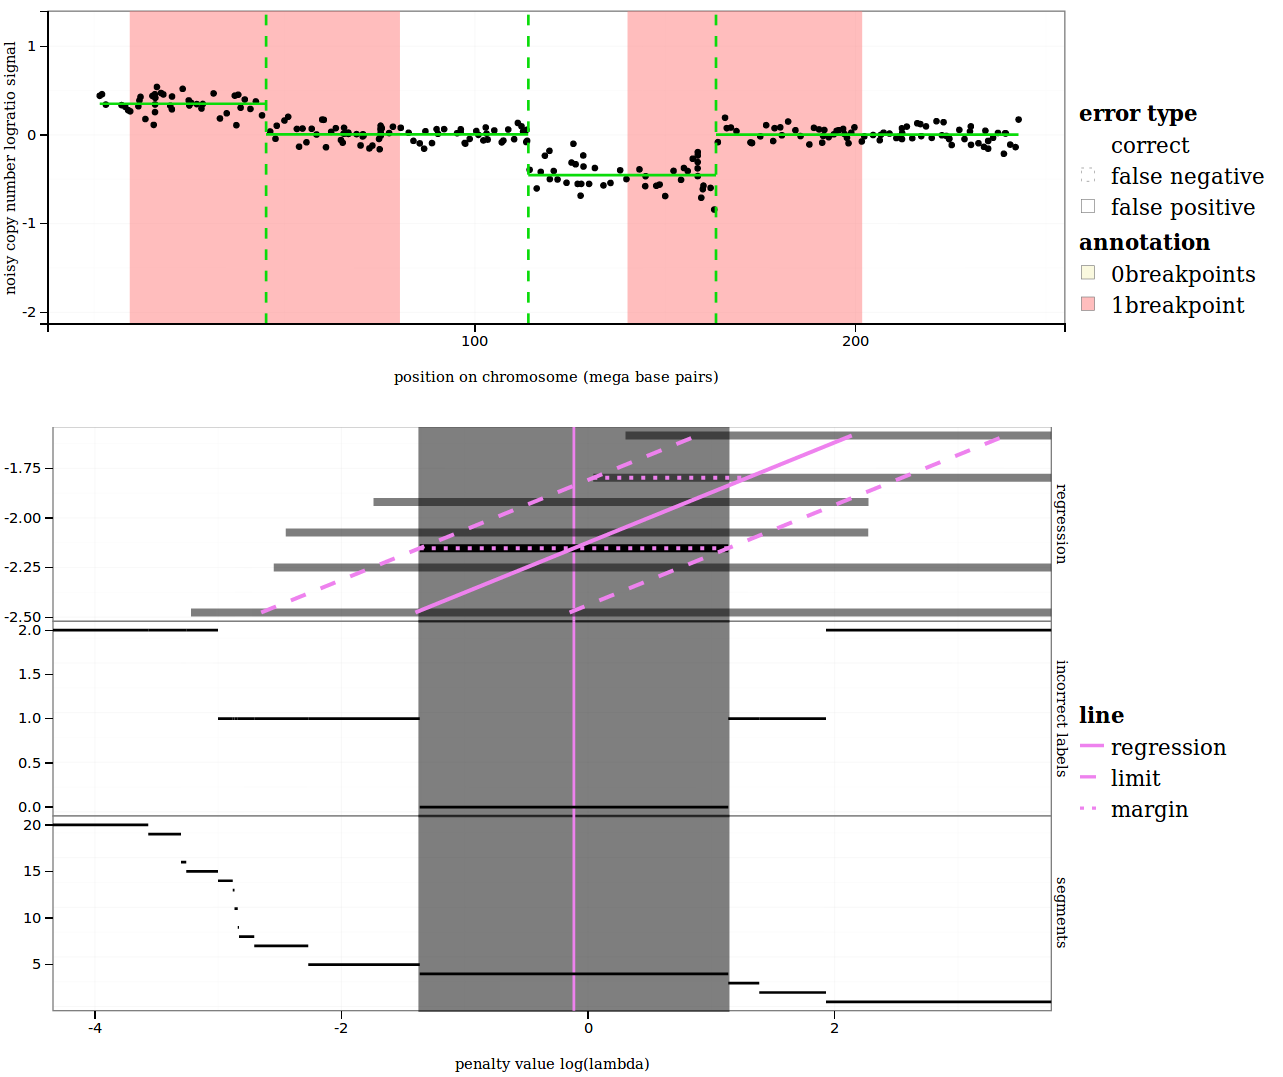
\includegraphics[height=0.8\textheight]{DNA-copy-number-analysis}

  \url{http://bl.ocks.org/tdhock/raw/10f27e4ace80bffa10a0/}
\end{frame}

\begin{frame}{Interval regression for ChIP-seq peak detection}
  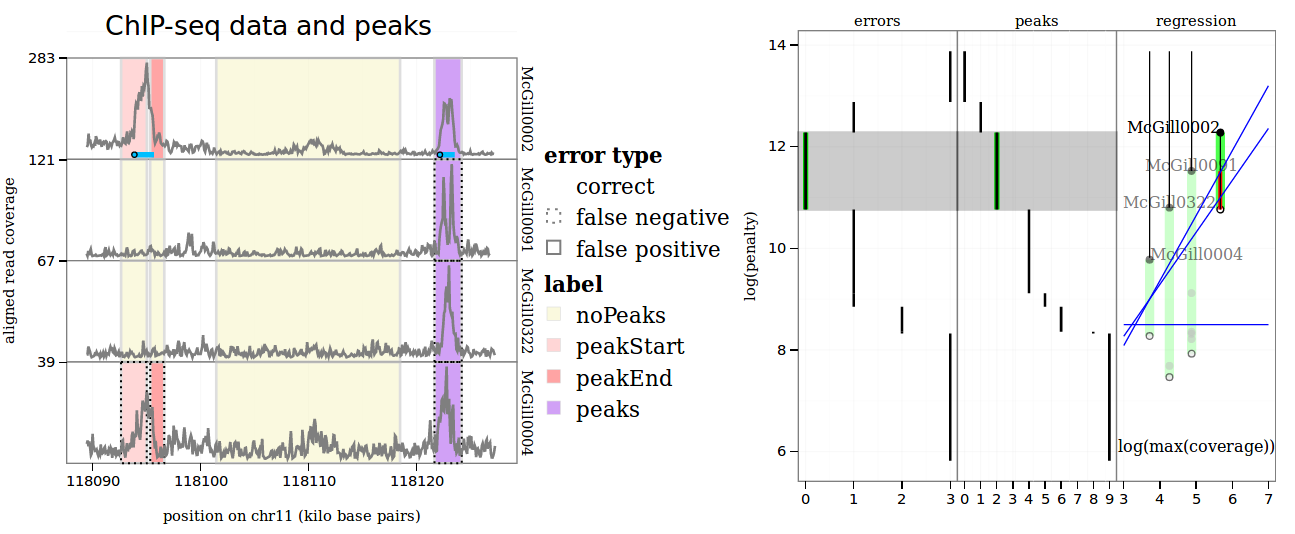
\includegraphics[width=\textwidth]{ChIP-seq-peak-detection}

  \small
  \url{http://bl.ocks.org/tdhock/raw/9311ca39d643d127e04a088814c81ee1/}
\end{frame}

\begin{frame}{A supervised learning problem}
	\begin{block}{Data set}
		\begin{equation*}
		\Scal \eqdef \{(\xb_1, \yb_1), (\xb_2, \yb_2), ..., (\xb_n, \yb_n))\} \sim D^n
		\end{equation*}
		$\xb \in \reals^p$ is a vector of \red{features}\\[2mm]
		$\yb_i \eqdef \left[ \, \ylower{i}, \yupper{i} \, \right]$, with $\ylower{i}, \yupper{i} \in \overline\reals$ and $\ylower{i} < \yupper{i}$, is an \red{interval}\\[2mm]
		$D$ is a \red{unknown} data generating distribution
	\end{block}
	\pause
	\vspace{2mm}
	\begin{block}{Censored data}
		\begin{itemize}
			\item<+-> Right censored: $\yb = [\ylower{i}, +\infty)$ \vspace{2mm}
			\item<+-> Left censored: $\yb = (-\infty, \yupper{i}]$ \vspace{2mm}
			\item<+-> Interval censored: $\yb = [\ylower{i}, \yupper{i}]$
		\end{itemize}
	\end{block}
\end{frame}

\begin{frame}{Measuring error with respect to an interval}
	\begin{block}{How do we measure the error?}
		Let $\mu \in \reals$ be the value predicted by some model. The error w.r.t. the interval $[\ylower{}, \yupper{}]$ is:	
		\vspace{-2mm}
		\begin{center}
			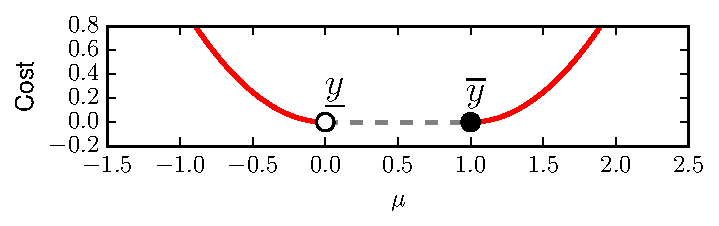
\includegraphics[scale=0.8]{figures/objective/interval_loss.pdf}
		\end{center}
	\end{block}
	\pause
	\begin{block}{Hinge loss}
		\begin{enumerate}
			\item<+-> Let $\ell: \reals \rightarrow \reals$ be any convex increasing function
			\item<+-> Let $[x]_+$, be the positive part function i.e. $[x]_+ \not = 0 \Leftrightarrow x > 0$
			\item<+-> The \emph{hinge loss} associated with $\ell$ is $\phi_\ell(x) = \ell([x]_+)$
		\end{enumerate}
	\end{block}
\end{frame}

\begin{frame}{Objective}
	Our goal is to find a function $f:\mathbb R^p\rightarrow\mathbb R$ that minimizes the expected error for any example drawn from $D$:
	$$
	\minimize_{f} \underset{(\xb_i, \yb_i) \sim D}{\mathbf{E}} \phi_\ell(\ylower{i} - f(\xb_i)) + \phi_\ell(f(\xb_i) - \yupper{i}),
	$$
	\vspace{6mm}
	\begin{center}
		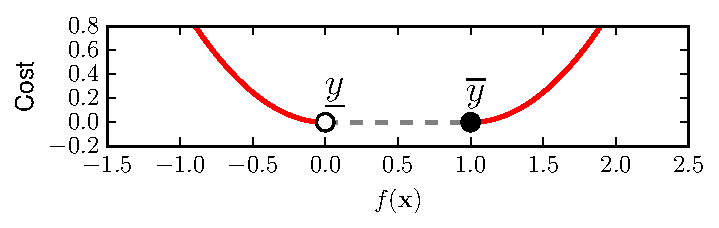
\includegraphics[scale=0.8]{figures/objective/interval_loss_fx.pdf}
	\end{center}
\end{frame}


\section{Maximum Margin Interval Trees}


\begin{frame}{Maximum Margin Interval Trees}
	\begin{itemize}
		\item<+-> We seek a regression tree $T: \reals^p \rightarrow \reals$ that minimizes:
		\begin{equation*}
		C(T) \eqdef \sum_{(\xb_i, \yb_i) \in S} \left[ \phi_\ell \left( - T(\xb_i) + \ylower{i} + \epsilon \right) + \phi_\ell \left(T(\xb_i) - \yupper{i} + \epsilon \right) \right]
		\end{equation*}\\[-2mm]
		where $\epsilon$ is a \red{margin hyperparameter} used for \red{regularization}.
		\vspace{5mm}
		\item<+-> We consider the cases $\ell(x) = x$ and $\ell(x) = x^2$.
	\end{itemize}
	\begin{center}
		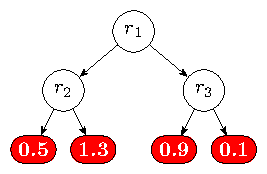
\includegraphics[scale=1.1]{figures/regression_tree/regression_tree.pdf}
	\end{center}
\end{frame}

\begin{frame}{The leaves of a MMIT}
	\begin{itemize}
		\item<+-> Let $\leaves{T}$ be the set of all leaves in a tree $T$
		\vspace{4mm}
		\item<+-> A leaf $\tau \in \leaves{T}$ is associated with a \red{set of examples} $S_\tau \subseteq S$ t.q.
			\begin{itemize}
				\item $S = \bigcup_{\tau \in \leaves{T}} S_\tau$
				\vspace{2mm}
				\item $S_\tau \cap S_{\tau'} \not= \emptyset \Leftrightarrow \tau = \tau'$
			\end{itemize}
		\vspace{4mm}
		\item<+-> Each leaf \red{predicts a constant value} for all the examples in $S_\tau$
		\vspace{4mm}
		\item<+-> The contribution of a leaf $\tau$ to the total cost of the tree, given that it predicts $\mu \in \reals$, is given by
		\begin{equation*}
		C_\tau(\mu) \eqdef \sum_{(\xb_i, \yb_i) \in S_\tau} \left[ \phi_\ell( - \mu + \ylower{i} + \epsilon) + \phi_\ell( \mu - \yupper{i} + \epsilon) \right]
		\end{equation*}
	\end{itemize}
\end{frame}

\begin{frame}{The tree is built by recursive partitioning}
	\begin{itemize}
		\item Let $\tau_0 \in \leaves{T}$ be any leaf:
		\begin{center}
			
\includegraphics[scale=1.2]{figures/leaf_split/root_leaf.pdf}
		\end{center}
		
		\vspace{6mm}
		
		\item We replace $\tau_0$ by two new leaves $\tau_1$ et $\tau_2$ according to a boolean-valued rule $r: \reals^p \rightarrow \{\text{True}, \text{False}\}$:
		\begin{center}
			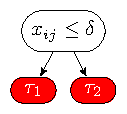
\includegraphics[scale=1.2]{figures/leaf_split/split_rule.pdf}
		\end{center}
		
	\end{itemize}
\end{frame}

\begin{frame}{Partitioning a leaf}
	\begin{center}
		\resizebox{\textwidth}{!}{%% Creator: Matplotlib, PGF backend
%%
%% To include the figure in your LaTeX document, write
%%   \input{<filename>.pgf}
%%
%% Make sure the required packages are loaded in your preamble
%%   \usepackage{pgf}
%%
%% Figures using additional raster images can only be included by \input if
%% they are in the same directory as the main LaTeX file. For loading figures
%% from other directories you can use the `import` package
%%   \usepackage{import}
%% and then include the figures with
%%   \import{<path to file>}{<filename>.pgf}
%%
%% Matplotlib used the following preamble
%%   \usepackage[utf8x]{inputenc}
%%   \usepackage[T1]{fontenc}
%%
\begingroup%
\makeatletter%
\begin{pgfpicture}%
\pgfpathrectangle{\pgfpointorigin}{\pgfqpoint{5.795114in}{2.132459in}}%
\pgfusepath{use as bounding box, clip}%
\begin{pgfscope}%
\pgfsetbuttcap%
\pgfsetmiterjoin%
\definecolor{currentfill}{rgb}{1.000000,1.000000,1.000000}%
\pgfsetfillcolor{currentfill}%
\pgfsetlinewidth{0.000000pt}%
\definecolor{currentstroke}{rgb}{1.000000,1.000000,1.000000}%
\pgfsetstrokecolor{currentstroke}%
\pgfsetdash{}{0pt}%
\pgfpathmoveto{\pgfqpoint{0.000000in}{-0.000000in}}%
\pgfpathlineto{\pgfqpoint{5.795114in}{-0.000000in}}%
\pgfpathlineto{\pgfqpoint{5.795114in}{2.132459in}}%
\pgfpathlineto{\pgfqpoint{0.000000in}{2.132459in}}%
\pgfpathclose%
\pgfusepath{fill}%
\end{pgfscope}%
\begin{pgfscope}%
\pgfsetbuttcap%
\pgfsetmiterjoin%
\definecolor{currentfill}{rgb}{1.000000,1.000000,1.000000}%
\pgfsetfillcolor{currentfill}%
\pgfsetlinewidth{0.000000pt}%
\definecolor{currentstroke}{rgb}{0.000000,0.000000,0.000000}%
\pgfsetstrokecolor{currentstroke}%
\pgfsetstrokeopacity{0.000000}%
\pgfsetdash{}{0pt}%
\pgfpathmoveto{\pgfqpoint{0.270114in}{0.285515in}}%
\pgfpathlineto{\pgfqpoint{2.781688in}{0.285515in}}%
\pgfpathlineto{\pgfqpoint{2.781688in}{1.685515in}}%
\pgfpathlineto{\pgfqpoint{0.270114in}{1.685515in}}%
\pgfpathclose%
\pgfusepath{fill}%
\end{pgfscope}%
\begin{pgfscope}%
\definecolor{textcolor}{rgb}{0.150000,0.150000,0.150000}%
\pgfsetstrokecolor{textcolor}%
\pgfsetfillcolor{textcolor}%
\pgftext[x=1.525901in,y=0.216070in,,top]{\color{textcolor}\sffamily\fontsize{8.000000}{9.600000}\selectfont Feature value (\(\displaystyle x_{ij}\))}%
\end{pgfscope}%
\begin{pgfscope}%
\definecolor{textcolor}{rgb}{0.150000,0.150000,0.150000}%
\pgfsetstrokecolor{textcolor}%
\pgfsetfillcolor{textcolor}%
\pgftext[x=0.200670in,y=0.985515in,,bottom,rotate=90.000000]{\color{textcolor}\sffamily\fontsize{8.000000}{9.600000}\selectfont Interval limits}%
\end{pgfscope}%
\begin{pgfscope}%
\pgfpathrectangle{\pgfqpoint{0.270114in}{0.285515in}}{\pgfqpoint{2.511574in}{1.400000in}} %
\pgfusepath{clip}%
\pgfsetbuttcap%
\pgfsetroundjoin%
\pgfsetlinewidth{1.003750pt}%
\definecolor{currentstroke}{rgb}{0.000000,0.501961,0.000000}%
\pgfsetstrokecolor{currentstroke}%
\pgfsetdash{{3.000000pt}{1.000000pt}{3.000000pt}{1.000000pt}}{0.000000pt}%
\pgfpathmoveto{\pgfqpoint{0.260114in}{1.004099in}}%
\pgfpathlineto{\pgfqpoint{2.791688in}{1.004099in}}%
\pgfusepath{stroke}%
\end{pgfscope}%
\begin{pgfscope}%
\pgfpathrectangle{\pgfqpoint{0.270114in}{0.285515in}}{\pgfqpoint{2.511574in}{1.400000in}} %
\pgfusepath{clip}%
\pgfsetbuttcap%
\pgfsetroundjoin%
\pgfsetlinewidth{1.003750pt}%
\definecolor{currentstroke}{rgb}{0.000000,0.000000,1.000000}%
\pgfsetstrokecolor{currentstroke}%
\pgfsetdash{{1.000000pt}{1.000000pt}{1.000000pt}{1.000000pt}}{0.000000pt}%
\pgfpathmoveto{\pgfqpoint{0.260114in}{0.880205in}}%
\pgfpathlineto{\pgfqpoint{2.791688in}{0.880205in}}%
\pgfusepath{stroke}%
\end{pgfscope}%
\begin{pgfscope}%
\pgfpathrectangle{\pgfqpoint{0.270114in}{0.285515in}}{\pgfqpoint{2.511574in}{1.400000in}} %
\pgfusepath{clip}%
\pgfsetbuttcap%
\pgfsetroundjoin%
\pgfsetlinewidth{1.003750pt}%
\definecolor{currentstroke}{rgb}{0.000000,0.000000,1.000000}%
\pgfsetstrokecolor{currentstroke}%
\pgfsetdash{{1.000000pt}{1.000000pt}{1.000000pt}{1.000000pt}}{0.000000pt}%
\pgfpathmoveto{\pgfqpoint{0.260114in}{1.127993in}}%
\pgfpathlineto{\pgfqpoint{2.791688in}{1.127993in}}%
\pgfusepath{stroke}%
\end{pgfscope}%
\begin{pgfscope}%
\definecolor{textcolor}{rgb}{0.150000,0.150000,0.150000}%
\pgfsetstrokecolor{textcolor}%
\pgfsetfillcolor{textcolor}%
\pgftext[x=0.284716in,y=1.028878in,left,base]{\color{textcolor}\sffamily\fontsize{8.000000}{9.600000}\selectfont \(\displaystyle \mu_0\)}%
\end{pgfscope}%
\begin{pgfscope}%
\definecolor{textcolor}{rgb}{0.150000,0.150000,0.150000}%
\pgfsetstrokecolor{textcolor}%
\pgfsetfillcolor{textcolor}%
\pgftext[x=0.430738in,y=1.047462in,left,base]{\color{textcolor}\sffamily\fontsize{8.000000}{9.600000}\selectfont \(\displaystyle \epsilon\)}%
\end{pgfscope}%
\begin{pgfscope}%
\definecolor{textcolor}{rgb}{0.150000,0.150000,0.150000}%
\pgfsetstrokecolor{textcolor}%
\pgfsetfillcolor{textcolor}%
\pgftext[x=0.430738in,y=0.942152in,left,base]{\color{textcolor}\sffamily\fontsize{8.000000}{9.600000}\selectfont \(\displaystyle \epsilon\)}%
\end{pgfscope}%
\begin{pgfscope}%
\pgfpathrectangle{\pgfqpoint{0.270114in}{0.285515in}}{\pgfqpoint{2.511574in}{1.400000in}} %
\pgfusepath{clip}%
\pgfsetbuttcap%
\pgfsetmiterjoin%
\definecolor{currentfill}{rgb}{0.000000,0.000000,0.000000}%
\pgfsetfillcolor{currentfill}%
\pgfsetlinewidth{0.301125pt}%
\definecolor{currentstroke}{rgb}{0.000000,0.000000,0.000000}%
\pgfsetstrokecolor{currentstroke}%
\pgfsetdash{}{0pt}%
\pgfpathmoveto{\pgfqpoint{0.423437in}{1.127993in}}%
\pgfpathlineto{\pgfqpoint{0.438039in}{1.103214in}}%
\pgfpathlineto{\pgfqpoint{0.423583in}{1.103214in}}%
\pgfpathlineto{\pgfqpoint{0.423583in}{1.004099in}}%
\pgfpathlineto{\pgfqpoint{0.423291in}{1.004099in}}%
\pgfpathlineto{\pgfqpoint{0.423291in}{1.103214in}}%
\pgfpathlineto{\pgfqpoint{0.408835in}{1.103214in}}%
\pgfpathclose%
\pgfusepath{stroke,fill}%
\end{pgfscope}%
\begin{pgfscope}%
\pgfpathrectangle{\pgfqpoint{0.270114in}{0.285515in}}{\pgfqpoint{2.511574in}{1.400000in}} %
\pgfusepath{clip}%
\pgfsetbuttcap%
\pgfsetmiterjoin%
\definecolor{currentfill}{rgb}{0.000000,0.000000,0.000000}%
\pgfsetfillcolor{currentfill}%
\pgfsetlinewidth{0.301125pt}%
\definecolor{currentstroke}{rgb}{0.000000,0.000000,0.000000}%
\pgfsetstrokecolor{currentstroke}%
\pgfsetdash{}{0pt}%
\pgfpathmoveto{\pgfqpoint{0.423437in}{0.880205in}}%
\pgfpathlineto{\pgfqpoint{0.408835in}{0.904984in}}%
\pgfpathlineto{\pgfqpoint{0.423291in}{0.904984in}}%
\pgfpathlineto{\pgfqpoint{0.423291in}{1.004099in}}%
\pgfpathlineto{\pgfqpoint{0.423583in}{1.004099in}}%
\pgfpathlineto{\pgfqpoint{0.423583in}{0.904984in}}%
\pgfpathlineto{\pgfqpoint{0.438039in}{0.904984in}}%
\pgfpathclose%
\pgfusepath{stroke,fill}%
\end{pgfscope}%
\begin{pgfscope}%
\pgfpathrectangle{\pgfqpoint{0.270114in}{0.285515in}}{\pgfqpoint{2.511574in}{1.400000in}} %
\pgfusepath{clip}%
\pgfsetbuttcap%
\pgfsetroundjoin%
\pgfsetlinewidth{1.003750pt}%
\definecolor{currentstroke}{rgb}{0.000000,0.000000,0.000000}%
\pgfsetstrokecolor{currentstroke}%
\pgfsetstrokeopacity{0.300000}%
\pgfsetdash{{1.000000pt}{2.000000pt}{3.000000pt}{1.000000pt}}{0.000000pt}%
\pgfpathmoveto{\pgfqpoint{0.503749in}{0.446577in}}%
\pgfpathlineto{\pgfqpoint{0.503749in}{1.189940in}}%
\pgfusepath{stroke}%
\end{pgfscope}%
\begin{pgfscope}%
\pgfpathrectangle{\pgfqpoint{0.270114in}{0.285515in}}{\pgfqpoint{2.511574in}{1.400000in}} %
\pgfusepath{clip}%
\pgfsetbuttcap%
\pgfsetroundjoin%
\pgfsetlinewidth{1.003750pt}%
\definecolor{currentstroke}{rgb}{1.000000,0.000000,0.000000}%
\pgfsetstrokecolor{currentstroke}%
\pgfsetdash{}{0pt}%
\pgfpathmoveto{\pgfqpoint{0.795793in}{0.570470in}}%
\pgfpathlineto{\pgfqpoint{0.795793in}{1.127993in}}%
\pgfusepath{stroke}%
\end{pgfscope}%
\begin{pgfscope}%
\pgfpathrectangle{\pgfqpoint{0.270114in}{0.285515in}}{\pgfqpoint{2.511574in}{1.400000in}} %
\pgfusepath{clip}%
\pgfsetbuttcap%
\pgfsetroundjoin%
\pgfsetlinewidth{1.003750pt}%
\definecolor{currentstroke}{rgb}{0.000000,0.000000,0.000000}%
\pgfsetstrokecolor{currentstroke}%
\pgfsetstrokeopacity{0.300000}%
\pgfsetdash{{1.000000pt}{2.000000pt}{3.000000pt}{1.000000pt}}{0.000000pt}%
\pgfpathmoveto{\pgfqpoint{0.795793in}{0.322683in}}%
\pgfpathlineto{\pgfqpoint{0.795793in}{0.570470in}}%
\pgfusepath{stroke}%
\end{pgfscope}%
\begin{pgfscope}%
\pgfpathrectangle{\pgfqpoint{0.270114in}{0.285515in}}{\pgfqpoint{2.511574in}{1.400000in}} %
\pgfusepath{clip}%
\pgfsetbuttcap%
\pgfsetroundjoin%
\pgfsetlinewidth{1.003750pt}%
\definecolor{currentstroke}{rgb}{1.000000,0.000000,0.000000}%
\pgfsetstrokecolor{currentstroke}%
\pgfsetdash{}{0pt}%
\pgfpathmoveto{\pgfqpoint{1.087836in}{0.942152in}}%
\pgfpathlineto{\pgfqpoint{1.087836in}{1.127993in}}%
\pgfusepath{stroke}%
\end{pgfscope}%
\begin{pgfscope}%
\pgfpathrectangle{\pgfqpoint{0.270114in}{0.285515in}}{\pgfqpoint{2.511574in}{1.400000in}} %
\pgfusepath{clip}%
\pgfsetbuttcap%
\pgfsetroundjoin%
\pgfsetlinewidth{1.003750pt}%
\definecolor{currentstroke}{rgb}{0.000000,0.000000,0.000000}%
\pgfsetstrokecolor{currentstroke}%
\pgfsetstrokeopacity{0.300000}%
\pgfsetdash{{1.000000pt}{2.000000pt}{3.000000pt}{1.000000pt}}{0.000000pt}%
\pgfpathmoveto{\pgfqpoint{1.087836in}{0.275515in}}%
\pgfpathlineto{\pgfqpoint{1.087836in}{0.942152in}}%
\pgfusepath{stroke}%
\end{pgfscope}%
\begin{pgfscope}%
\pgfpathrectangle{\pgfqpoint{0.270114in}{0.285515in}}{\pgfqpoint{2.511574in}{1.400000in}} %
\pgfusepath{clip}%
\pgfsetbuttcap%
\pgfsetroundjoin%
\pgfsetlinewidth{1.003750pt}%
\definecolor{currentstroke}{rgb}{1.000000,0.000000,0.000000}%
\pgfsetstrokecolor{currentstroke}%
\pgfsetdash{}{0pt}%
\pgfpathmoveto{\pgfqpoint{1.379880in}{1.066046in}}%
\pgfpathlineto{\pgfqpoint{1.379880in}{1.127993in}}%
\pgfusepath{stroke}%
\end{pgfscope}%
\begin{pgfscope}%
\pgfpathrectangle{\pgfqpoint{0.270114in}{0.285515in}}{\pgfqpoint{2.511574in}{1.400000in}} %
\pgfusepath{clip}%
\pgfsetbuttcap%
\pgfsetroundjoin%
\pgfsetlinewidth{1.003750pt}%
\definecolor{currentstroke}{rgb}{0.000000,0.000000,0.000000}%
\pgfsetstrokecolor{currentstroke}%
\pgfsetstrokeopacity{0.300000}%
\pgfsetdash{{1.000000pt}{2.000000pt}{3.000000pt}{1.000000pt}}{0.000000pt}%
\pgfpathmoveto{\pgfqpoint{1.379880in}{0.694364in}}%
\pgfpathlineto{\pgfqpoint{1.379880in}{1.066046in}}%
\pgfusepath{stroke}%
\end{pgfscope}%
\begin{pgfscope}%
\pgfpathrectangle{\pgfqpoint{0.270114in}{0.285515in}}{\pgfqpoint{2.511574in}{1.400000in}} %
\pgfusepath{clip}%
\pgfsetbuttcap%
\pgfsetroundjoin%
\pgfsetlinewidth{1.003750pt}%
\definecolor{currentstroke}{rgb}{1.000000,0.000000,0.000000}%
\pgfsetstrokecolor{currentstroke}%
\pgfsetdash{}{0pt}%
\pgfpathmoveto{\pgfqpoint{1.671923in}{0.942152in}}%
\pgfpathlineto{\pgfqpoint{1.671923in}{0.880205in}}%
\pgfusepath{stroke}%
\end{pgfscope}%
\begin{pgfscope}%
\pgfpathrectangle{\pgfqpoint{0.270114in}{0.285515in}}{\pgfqpoint{2.511574in}{1.400000in}} %
\pgfusepath{clip}%
\pgfsetbuttcap%
\pgfsetroundjoin%
\pgfsetlinewidth{1.003750pt}%
\definecolor{currentstroke}{rgb}{0.000000,0.000000,0.000000}%
\pgfsetstrokecolor{currentstroke}%
\pgfsetstrokeopacity{0.300000}%
\pgfsetdash{{1.000000pt}{2.000000pt}{3.000000pt}{1.000000pt}}{0.000000pt}%
\pgfpathmoveto{\pgfqpoint{1.671923in}{0.942152in}}%
\pgfpathlineto{\pgfqpoint{1.671923in}{1.313833in}}%
\pgfusepath{stroke}%
\end{pgfscope}%
\begin{pgfscope}%
\pgfpathrectangle{\pgfqpoint{0.270114in}{0.285515in}}{\pgfqpoint{2.511574in}{1.400000in}} %
\pgfusepath{clip}%
\pgfsetbuttcap%
\pgfsetroundjoin%
\pgfsetlinewidth{1.003750pt}%
\definecolor{currentstroke}{rgb}{1.000000,0.000000,0.000000}%
\pgfsetstrokecolor{currentstroke}%
\pgfsetdash{}{0pt}%
\pgfpathmoveto{\pgfqpoint{1.963967in}{1.158966in}}%
\pgfpathlineto{\pgfqpoint{1.963967in}{0.880205in}}%
\pgfusepath{stroke}%
\end{pgfscope}%
\begin{pgfscope}%
\pgfpathrectangle{\pgfqpoint{0.270114in}{0.285515in}}{\pgfqpoint{2.511574in}{1.400000in}} %
\pgfusepath{clip}%
\pgfsetbuttcap%
\pgfsetroundjoin%
\pgfsetlinewidth{1.003750pt}%
\definecolor{currentstroke}{rgb}{0.000000,0.000000,0.000000}%
\pgfsetstrokecolor{currentstroke}%
\pgfsetstrokeopacity{0.300000}%
\pgfsetdash{{1.000000pt}{2.000000pt}{3.000000pt}{1.000000pt}}{0.000000pt}%
\pgfpathmoveto{\pgfqpoint{1.963967in}{1.158966in}}%
\pgfpathlineto{\pgfqpoint{1.963967in}{1.695515in}}%
\pgfusepath{stroke}%
\end{pgfscope}%
\begin{pgfscope}%
\pgfpathrectangle{\pgfqpoint{0.270114in}{0.285515in}}{\pgfqpoint{2.511574in}{1.400000in}} %
\pgfusepath{clip}%
\pgfsetbuttcap%
\pgfsetroundjoin%
\pgfsetlinewidth{1.003750pt}%
\definecolor{currentstroke}{rgb}{1.000000,0.000000,0.000000}%
\pgfsetstrokecolor{currentstroke}%
\pgfsetdash{}{0pt}%
\pgfpathmoveto{\pgfqpoint{2.256010in}{1.035072in}}%
\pgfpathlineto{\pgfqpoint{2.256010in}{0.880205in}}%
\pgfusepath{stroke}%
\end{pgfscope}%
\begin{pgfscope}%
\pgfpathrectangle{\pgfqpoint{0.270114in}{0.285515in}}{\pgfqpoint{2.511574in}{1.400000in}} %
\pgfusepath{clip}%
\pgfsetbuttcap%
\pgfsetroundjoin%
\pgfsetlinewidth{1.003750pt}%
\definecolor{currentstroke}{rgb}{0.000000,0.000000,0.000000}%
\pgfsetstrokecolor{currentstroke}%
\pgfsetstrokeopacity{0.300000}%
\pgfsetdash{{1.000000pt}{2.000000pt}{3.000000pt}{1.000000pt}}{0.000000pt}%
\pgfpathmoveto{\pgfqpoint{2.256010in}{1.035072in}}%
\pgfpathlineto{\pgfqpoint{2.256010in}{1.437727in}}%
\pgfusepath{stroke}%
\end{pgfscope}%
\begin{pgfscope}%
\pgfpathrectangle{\pgfqpoint{0.270114in}{0.285515in}}{\pgfqpoint{2.511574in}{1.400000in}} %
\pgfusepath{clip}%
\pgfsetbuttcap%
\pgfsetroundjoin%
\pgfsetlinewidth{1.003750pt}%
\definecolor{currentstroke}{rgb}{1.000000,0.000000,0.000000}%
\pgfsetstrokecolor{currentstroke}%
\pgfsetdash{}{0pt}%
\pgfpathmoveto{\pgfqpoint{2.548054in}{0.942152in}}%
\pgfpathlineto{\pgfqpoint{2.548054in}{0.880205in}}%
\pgfusepath{stroke}%
\end{pgfscope}%
\begin{pgfscope}%
\pgfpathrectangle{\pgfqpoint{0.270114in}{0.285515in}}{\pgfqpoint{2.511574in}{1.400000in}} %
\pgfusepath{clip}%
\pgfsetbuttcap%
\pgfsetroundjoin%
\pgfsetlinewidth{1.003750pt}%
\definecolor{currentstroke}{rgb}{0.000000,0.000000,0.000000}%
\pgfsetstrokecolor{currentstroke}%
\pgfsetstrokeopacity{0.300000}%
\pgfsetdash{{1.000000pt}{2.000000pt}{3.000000pt}{1.000000pt}}{0.000000pt}%
\pgfpathmoveto{\pgfqpoint{2.548054in}{0.942152in}}%
\pgfpathlineto{\pgfqpoint{2.548054in}{1.437727in}}%
\pgfusepath{stroke}%
\end{pgfscope}%
\begin{pgfscope}%
\pgfsetrectcap%
\pgfsetmiterjoin%
\pgfsetlinewidth{1.254687pt}%
\definecolor{currentstroke}{rgb}{0.150000,0.150000,0.150000}%
\pgfsetstrokecolor{currentstroke}%
\pgfsetdash{}{0pt}%
\pgfpathmoveto{\pgfqpoint{0.270114in}{1.685515in}}%
\pgfpathlineto{\pgfqpoint{2.781688in}{1.685515in}}%
\pgfusepath{stroke}%
\end{pgfscope}%
\begin{pgfscope}%
\pgfsetrectcap%
\pgfsetmiterjoin%
\pgfsetlinewidth{1.254687pt}%
\definecolor{currentstroke}{rgb}{0.150000,0.150000,0.150000}%
\pgfsetstrokecolor{currentstroke}%
\pgfsetdash{}{0pt}%
\pgfpathmoveto{\pgfqpoint{2.781688in}{0.285515in}}%
\pgfpathlineto{\pgfqpoint{2.781688in}{1.685515in}}%
\pgfusepath{stroke}%
\end{pgfscope}%
\begin{pgfscope}%
\pgfsetrectcap%
\pgfsetmiterjoin%
\pgfsetlinewidth{1.254687pt}%
\definecolor{currentstroke}{rgb}{0.150000,0.150000,0.150000}%
\pgfsetstrokecolor{currentstroke}%
\pgfsetdash{}{0pt}%
\pgfpathmoveto{\pgfqpoint{0.270114in}{0.285515in}}%
\pgfpathlineto{\pgfqpoint{2.781688in}{0.285515in}}%
\pgfusepath{stroke}%
\end{pgfscope}%
\begin{pgfscope}%
\pgfsetrectcap%
\pgfsetmiterjoin%
\pgfsetlinewidth{1.254687pt}%
\definecolor{currentstroke}{rgb}{0.150000,0.150000,0.150000}%
\pgfsetstrokecolor{currentstroke}%
\pgfsetdash{}{0pt}%
\pgfpathmoveto{\pgfqpoint{0.270114in}{0.285515in}}%
\pgfpathlineto{\pgfqpoint{0.270114in}{1.685515in}}%
\pgfusepath{stroke}%
\end{pgfscope}%
\begin{pgfscope}%
\pgfpathrectangle{\pgfqpoint{0.270114in}{0.285515in}}{\pgfqpoint{2.511574in}{1.400000in}} %
\pgfusepath{clip}%
\pgfsetbuttcap%
\pgfsetroundjoin%
\definecolor{currentfill}{rgb}{1.000000,1.000000,1.000000}%
\pgfsetfillcolor{currentfill}%
\pgfsetlinewidth{1.003750pt}%
\definecolor{currentstroke}{rgb}{0.000000,0.000000,0.000000}%
\pgfsetstrokecolor{currentstroke}%
\pgfsetdash{}{0pt}%
\pgfpathmoveto{\pgfqpoint{0.503749in}{0.415520in}}%
\pgfpathcurveto{\pgfqpoint{0.511985in}{0.415520in}}{\pgfqpoint{0.519885in}{0.418792in}}{\pgfqpoint{0.525709in}{0.424616in}}%
\pgfpathcurveto{\pgfqpoint{0.531533in}{0.430440in}}{\pgfqpoint{0.534806in}{0.438340in}}{\pgfqpoint{0.534806in}{0.446577in}}%
\pgfpathcurveto{\pgfqpoint{0.534806in}{0.454813in}}{\pgfqpoint{0.531533in}{0.462713in}}{\pgfqpoint{0.525709in}{0.468537in}}%
\pgfpathcurveto{\pgfqpoint{0.519885in}{0.474361in}}{\pgfqpoint{0.511985in}{0.477633in}}{\pgfqpoint{0.503749in}{0.477633in}}%
\pgfpathcurveto{\pgfqpoint{0.495513in}{0.477633in}}{\pgfqpoint{0.487613in}{0.474361in}}{\pgfqpoint{0.481789in}{0.468537in}}%
\pgfpathcurveto{\pgfqpoint{0.475965in}{0.462713in}}{\pgfqpoint{0.472693in}{0.454813in}}{\pgfqpoint{0.472693in}{0.446577in}}%
\pgfpathcurveto{\pgfqpoint{0.472693in}{0.438340in}}{\pgfqpoint{0.475965in}{0.430440in}}{\pgfqpoint{0.481789in}{0.424616in}}%
\pgfpathcurveto{\pgfqpoint{0.487613in}{0.418792in}}{\pgfqpoint{0.495513in}{0.415520in}}{\pgfqpoint{0.503749in}{0.415520in}}%
\pgfpathclose%
\pgfusepath{stroke,fill}%
\end{pgfscope}%
\begin{pgfscope}%
\pgfpathrectangle{\pgfqpoint{0.270114in}{0.285515in}}{\pgfqpoint{2.511574in}{1.400000in}} %
\pgfusepath{clip}%
\pgfsetbuttcap%
\pgfsetroundjoin%
\definecolor{currentfill}{rgb}{0.000000,0.000000,0.000000}%
\pgfsetfillcolor{currentfill}%
\pgfsetlinewidth{1.003750pt}%
\definecolor{currentstroke}{rgb}{0.000000,0.000000,0.000000}%
\pgfsetstrokecolor{currentstroke}%
\pgfsetdash{}{0pt}%
\pgfpathmoveto{\pgfqpoint{0.503749in}{1.158883in}}%
\pgfpathcurveto{\pgfqpoint{0.511985in}{1.158883in}}{\pgfqpoint{0.519885in}{1.162155in}}{\pgfqpoint{0.525709in}{1.167979in}}%
\pgfpathcurveto{\pgfqpoint{0.531533in}{1.173803in}}{\pgfqpoint{0.534806in}{1.181703in}}{\pgfqpoint{0.534806in}{1.189940in}}%
\pgfpathcurveto{\pgfqpoint{0.534806in}{1.198176in}}{\pgfqpoint{0.531533in}{1.206076in}}{\pgfqpoint{0.525709in}{1.211900in}}%
\pgfpathcurveto{\pgfqpoint{0.519885in}{1.217724in}}{\pgfqpoint{0.511985in}{1.220996in}}{\pgfqpoint{0.503749in}{1.220996in}}%
\pgfpathcurveto{\pgfqpoint{0.495513in}{1.220996in}}{\pgfqpoint{0.487613in}{1.217724in}}{\pgfqpoint{0.481789in}{1.211900in}}%
\pgfpathcurveto{\pgfqpoint{0.475965in}{1.206076in}}{\pgfqpoint{0.472693in}{1.198176in}}{\pgfqpoint{0.472693in}{1.189940in}}%
\pgfpathcurveto{\pgfqpoint{0.472693in}{1.181703in}}{\pgfqpoint{0.475965in}{1.173803in}}{\pgfqpoint{0.481789in}{1.167979in}}%
\pgfpathcurveto{\pgfqpoint{0.487613in}{1.162155in}}{\pgfqpoint{0.495513in}{1.158883in}}{\pgfqpoint{0.503749in}{1.158883in}}%
\pgfpathclose%
\pgfusepath{stroke,fill}%
\end{pgfscope}%
\begin{pgfscope}%
\pgfpathrectangle{\pgfqpoint{0.270114in}{0.285515in}}{\pgfqpoint{2.511574in}{1.400000in}} %
\pgfusepath{clip}%
\pgfsetbuttcap%
\pgfsetroundjoin%
\definecolor{currentfill}{rgb}{1.000000,1.000000,1.000000}%
\pgfsetfillcolor{currentfill}%
\pgfsetlinewidth{1.003750pt}%
\definecolor{currentstroke}{rgb}{0.000000,0.000000,0.000000}%
\pgfsetstrokecolor{currentstroke}%
\pgfsetdash{}{0pt}%
\pgfpathmoveto{\pgfqpoint{0.795793in}{0.291626in}}%
\pgfpathcurveto{\pgfqpoint{0.804029in}{0.291626in}}{\pgfqpoint{0.811929in}{0.294899in}}{\pgfqpoint{0.817753in}{0.300723in}}%
\pgfpathcurveto{\pgfqpoint{0.823577in}{0.306547in}}{\pgfqpoint{0.826849in}{0.314447in}}{\pgfqpoint{0.826849in}{0.322683in}}%
\pgfpathcurveto{\pgfqpoint{0.826849in}{0.330919in}}{\pgfqpoint{0.823577in}{0.338819in}}{\pgfqpoint{0.817753in}{0.344643in}}%
\pgfpathcurveto{\pgfqpoint{0.811929in}{0.350467in}}{\pgfqpoint{0.804029in}{0.353739in}}{\pgfqpoint{0.795793in}{0.353739in}}%
\pgfpathcurveto{\pgfqpoint{0.787556in}{0.353739in}}{\pgfqpoint{0.779656in}{0.350467in}}{\pgfqpoint{0.773832in}{0.344643in}}%
\pgfpathcurveto{\pgfqpoint{0.768008in}{0.338819in}}{\pgfqpoint{0.764736in}{0.330919in}}{\pgfqpoint{0.764736in}{0.322683in}}%
\pgfpathcurveto{\pgfqpoint{0.764736in}{0.314447in}}{\pgfqpoint{0.768008in}{0.306547in}}{\pgfqpoint{0.773832in}{0.300723in}}%
\pgfpathcurveto{\pgfqpoint{0.779656in}{0.294899in}}{\pgfqpoint{0.787556in}{0.291626in}}{\pgfqpoint{0.795793in}{0.291626in}}%
\pgfpathclose%
\pgfusepath{stroke,fill}%
\end{pgfscope}%
\begin{pgfscope}%
\pgfpathrectangle{\pgfqpoint{0.270114in}{0.285515in}}{\pgfqpoint{2.511574in}{1.400000in}} %
\pgfusepath{clip}%
\pgfsetbuttcap%
\pgfsetroundjoin%
\definecolor{currentfill}{rgb}{0.000000,0.000000,0.000000}%
\pgfsetfillcolor{currentfill}%
\pgfsetlinewidth{1.003750pt}%
\definecolor{currentstroke}{rgb}{0.000000,0.000000,0.000000}%
\pgfsetstrokecolor{currentstroke}%
\pgfsetdash{}{0pt}%
\pgfpathmoveto{\pgfqpoint{0.795793in}{0.539414in}}%
\pgfpathcurveto{\pgfqpoint{0.804029in}{0.539414in}}{\pgfqpoint{0.811929in}{0.542686in}}{\pgfqpoint{0.817753in}{0.548510in}}%
\pgfpathcurveto{\pgfqpoint{0.823577in}{0.554334in}}{\pgfqpoint{0.826849in}{0.562234in}}{\pgfqpoint{0.826849in}{0.570470in}}%
\pgfpathcurveto{\pgfqpoint{0.826849in}{0.578707in}}{\pgfqpoint{0.823577in}{0.586607in}}{\pgfqpoint{0.817753in}{0.592431in}}%
\pgfpathcurveto{\pgfqpoint{0.811929in}{0.598255in}}{\pgfqpoint{0.804029in}{0.601527in}}{\pgfqpoint{0.795793in}{0.601527in}}%
\pgfpathcurveto{\pgfqpoint{0.787556in}{0.601527in}}{\pgfqpoint{0.779656in}{0.598255in}}{\pgfqpoint{0.773832in}{0.592431in}}%
\pgfpathcurveto{\pgfqpoint{0.768008in}{0.586607in}}{\pgfqpoint{0.764736in}{0.578707in}}{\pgfqpoint{0.764736in}{0.570470in}}%
\pgfpathcurveto{\pgfqpoint{0.764736in}{0.562234in}}{\pgfqpoint{0.768008in}{0.554334in}}{\pgfqpoint{0.773832in}{0.548510in}}%
\pgfpathcurveto{\pgfqpoint{0.779656in}{0.542686in}}{\pgfqpoint{0.787556in}{0.539414in}}{\pgfqpoint{0.795793in}{0.539414in}}%
\pgfpathclose%
\pgfusepath{stroke,fill}%
\end{pgfscope}%
\begin{pgfscope}%
\pgfpathrectangle{\pgfqpoint{0.270114in}{0.285515in}}{\pgfqpoint{2.511574in}{1.400000in}} %
\pgfusepath{clip}%
\pgfsetbuttcap%
\pgfsetroundjoin%
\definecolor{currentfill}{rgb}{0.000000,0.000000,0.000000}%
\pgfsetfillcolor{currentfill}%
\pgfsetlinewidth{1.003750pt}%
\definecolor{currentstroke}{rgb}{0.000000,0.000000,0.000000}%
\pgfsetstrokecolor{currentstroke}%
\pgfsetdash{}{0pt}%
\pgfpathmoveto{\pgfqpoint{1.087836in}{0.911095in}}%
\pgfpathcurveto{\pgfqpoint{1.096072in}{0.911095in}}{\pgfqpoint{1.103972in}{0.914368in}}{\pgfqpoint{1.109796in}{0.920192in}}%
\pgfpathcurveto{\pgfqpoint{1.115620in}{0.926016in}}{\pgfqpoint{1.118893in}{0.933916in}}{\pgfqpoint{1.118893in}{0.942152in}}%
\pgfpathcurveto{\pgfqpoint{1.118893in}{0.950388in}}{\pgfqpoint{1.115620in}{0.958288in}}{\pgfqpoint{1.109796in}{0.964112in}}%
\pgfpathcurveto{\pgfqpoint{1.103972in}{0.969936in}}{\pgfqpoint{1.096072in}{0.973208in}}{\pgfqpoint{1.087836in}{0.973208in}}%
\pgfpathcurveto{\pgfqpoint{1.079600in}{0.973208in}}{\pgfqpoint{1.071700in}{0.969936in}}{\pgfqpoint{1.065876in}{0.964112in}}%
\pgfpathcurveto{\pgfqpoint{1.060052in}{0.958288in}}{\pgfqpoint{1.056780in}{0.950388in}}{\pgfqpoint{1.056780in}{0.942152in}}%
\pgfpathcurveto{\pgfqpoint{1.056780in}{0.933916in}}{\pgfqpoint{1.060052in}{0.926016in}}{\pgfqpoint{1.065876in}{0.920192in}}%
\pgfpathcurveto{\pgfqpoint{1.071700in}{0.914368in}}{\pgfqpoint{1.079600in}{0.911095in}}{\pgfqpoint{1.087836in}{0.911095in}}%
\pgfpathclose%
\pgfusepath{stroke,fill}%
\end{pgfscope}%
\begin{pgfscope}%
\pgfpathrectangle{\pgfqpoint{0.270114in}{0.285515in}}{\pgfqpoint{2.511574in}{1.400000in}} %
\pgfusepath{clip}%
\pgfsetbuttcap%
\pgfsetroundjoin%
\definecolor{currentfill}{rgb}{1.000000,1.000000,1.000000}%
\pgfsetfillcolor{currentfill}%
\pgfsetlinewidth{1.003750pt}%
\definecolor{currentstroke}{rgb}{0.000000,0.000000,0.000000}%
\pgfsetstrokecolor{currentstroke}%
\pgfsetdash{}{0pt}%
\pgfpathmoveto{\pgfqpoint{1.379880in}{0.663308in}}%
\pgfpathcurveto{\pgfqpoint{1.388116in}{0.663308in}}{\pgfqpoint{1.396016in}{0.666580in}}{\pgfqpoint{1.401840in}{0.672404in}}%
\pgfpathcurveto{\pgfqpoint{1.407664in}{0.678228in}}{\pgfqpoint{1.410936in}{0.686128in}}{\pgfqpoint{1.410936in}{0.694364in}}%
\pgfpathcurveto{\pgfqpoint{1.410936in}{0.702601in}}{\pgfqpoint{1.407664in}{0.710501in}}{\pgfqpoint{1.401840in}{0.716325in}}%
\pgfpathcurveto{\pgfqpoint{1.396016in}{0.722148in}}{\pgfqpoint{1.388116in}{0.725421in}}{\pgfqpoint{1.379880in}{0.725421in}}%
\pgfpathcurveto{\pgfqpoint{1.371643in}{0.725421in}}{\pgfqpoint{1.363743in}{0.722148in}}{\pgfqpoint{1.357919in}{0.716325in}}%
\pgfpathcurveto{\pgfqpoint{1.352095in}{0.710501in}}{\pgfqpoint{1.348823in}{0.702601in}}{\pgfqpoint{1.348823in}{0.694364in}}%
\pgfpathcurveto{\pgfqpoint{1.348823in}{0.686128in}}{\pgfqpoint{1.352095in}{0.678228in}}{\pgfqpoint{1.357919in}{0.672404in}}%
\pgfpathcurveto{\pgfqpoint{1.363743in}{0.666580in}}{\pgfqpoint{1.371643in}{0.663308in}}{\pgfqpoint{1.379880in}{0.663308in}}%
\pgfpathclose%
\pgfusepath{stroke,fill}%
\end{pgfscope}%
\begin{pgfscope}%
\pgfpathrectangle{\pgfqpoint{0.270114in}{0.285515in}}{\pgfqpoint{2.511574in}{1.400000in}} %
\pgfusepath{clip}%
\pgfsetbuttcap%
\pgfsetroundjoin%
\definecolor{currentfill}{rgb}{0.000000,0.000000,0.000000}%
\pgfsetfillcolor{currentfill}%
\pgfsetlinewidth{1.003750pt}%
\definecolor{currentstroke}{rgb}{0.000000,0.000000,0.000000}%
\pgfsetstrokecolor{currentstroke}%
\pgfsetdash{}{0pt}%
\pgfpathmoveto{\pgfqpoint{1.379880in}{1.034989in}}%
\pgfpathcurveto{\pgfqpoint{1.388116in}{1.034989in}}{\pgfqpoint{1.396016in}{1.038262in}}{\pgfqpoint{1.401840in}{1.044085in}}%
\pgfpathcurveto{\pgfqpoint{1.407664in}{1.049909in}}{\pgfqpoint{1.410936in}{1.057809in}}{\pgfqpoint{1.410936in}{1.066046in}}%
\pgfpathcurveto{\pgfqpoint{1.410936in}{1.074282in}}{\pgfqpoint{1.407664in}{1.082182in}}{\pgfqpoint{1.401840in}{1.088006in}}%
\pgfpathcurveto{\pgfqpoint{1.396016in}{1.093830in}}{\pgfqpoint{1.388116in}{1.097102in}}{\pgfqpoint{1.379880in}{1.097102in}}%
\pgfpathcurveto{\pgfqpoint{1.371643in}{1.097102in}}{\pgfqpoint{1.363743in}{1.093830in}}{\pgfqpoint{1.357919in}{1.088006in}}%
\pgfpathcurveto{\pgfqpoint{1.352095in}{1.082182in}}{\pgfqpoint{1.348823in}{1.074282in}}{\pgfqpoint{1.348823in}{1.066046in}}%
\pgfpathcurveto{\pgfqpoint{1.348823in}{1.057809in}}{\pgfqpoint{1.352095in}{1.049909in}}{\pgfqpoint{1.357919in}{1.044085in}}%
\pgfpathcurveto{\pgfqpoint{1.363743in}{1.038262in}}{\pgfqpoint{1.371643in}{1.034989in}}{\pgfqpoint{1.379880in}{1.034989in}}%
\pgfpathclose%
\pgfusepath{stroke,fill}%
\end{pgfscope}%
\begin{pgfscope}%
\pgfpathrectangle{\pgfqpoint{0.270114in}{0.285515in}}{\pgfqpoint{2.511574in}{1.400000in}} %
\pgfusepath{clip}%
\pgfsetbuttcap%
\pgfsetroundjoin%
\definecolor{currentfill}{rgb}{1.000000,1.000000,1.000000}%
\pgfsetfillcolor{currentfill}%
\pgfsetlinewidth{1.003750pt}%
\definecolor{currentstroke}{rgb}{0.000000,0.000000,0.000000}%
\pgfsetstrokecolor{currentstroke}%
\pgfsetdash{}{0pt}%
\pgfpathmoveto{\pgfqpoint{1.671923in}{0.911095in}}%
\pgfpathcurveto{\pgfqpoint{1.680159in}{0.911095in}}{\pgfqpoint{1.688059in}{0.914368in}}{\pgfqpoint{1.693883in}{0.920192in}}%
\pgfpathcurveto{\pgfqpoint{1.699707in}{0.926016in}}{\pgfqpoint{1.702980in}{0.933916in}}{\pgfqpoint{1.702980in}{0.942152in}}%
\pgfpathcurveto{\pgfqpoint{1.702980in}{0.950388in}}{\pgfqpoint{1.699707in}{0.958288in}}{\pgfqpoint{1.693883in}{0.964112in}}%
\pgfpathcurveto{\pgfqpoint{1.688059in}{0.969936in}}{\pgfqpoint{1.680159in}{0.973208in}}{\pgfqpoint{1.671923in}{0.973208in}}%
\pgfpathcurveto{\pgfqpoint{1.663687in}{0.973208in}}{\pgfqpoint{1.655787in}{0.969936in}}{\pgfqpoint{1.649963in}{0.964112in}}%
\pgfpathcurveto{\pgfqpoint{1.644139in}{0.958288in}}{\pgfqpoint{1.640867in}{0.950388in}}{\pgfqpoint{1.640867in}{0.942152in}}%
\pgfpathcurveto{\pgfqpoint{1.640867in}{0.933916in}}{\pgfqpoint{1.644139in}{0.926016in}}{\pgfqpoint{1.649963in}{0.920192in}}%
\pgfpathcurveto{\pgfqpoint{1.655787in}{0.914368in}}{\pgfqpoint{1.663687in}{0.911095in}}{\pgfqpoint{1.671923in}{0.911095in}}%
\pgfpathclose%
\pgfusepath{stroke,fill}%
\end{pgfscope}%
\begin{pgfscope}%
\pgfpathrectangle{\pgfqpoint{0.270114in}{0.285515in}}{\pgfqpoint{2.511574in}{1.400000in}} %
\pgfusepath{clip}%
\pgfsetbuttcap%
\pgfsetroundjoin%
\definecolor{currentfill}{rgb}{0.000000,0.000000,0.000000}%
\pgfsetfillcolor{currentfill}%
\pgfsetlinewidth{1.003750pt}%
\definecolor{currentstroke}{rgb}{0.000000,0.000000,0.000000}%
\pgfsetstrokecolor{currentstroke}%
\pgfsetdash{}{0pt}%
\pgfpathmoveto{\pgfqpoint{1.671923in}{1.282777in}}%
\pgfpathcurveto{\pgfqpoint{1.680159in}{1.282777in}}{\pgfqpoint{1.688059in}{1.286049in}}{\pgfqpoint{1.693883in}{1.291873in}}%
\pgfpathcurveto{\pgfqpoint{1.699707in}{1.297697in}}{\pgfqpoint{1.702980in}{1.305597in}}{\pgfqpoint{1.702980in}{1.313833in}}%
\pgfpathcurveto{\pgfqpoint{1.702980in}{1.322070in}}{\pgfqpoint{1.699707in}{1.329970in}}{\pgfqpoint{1.693883in}{1.335794in}}%
\pgfpathcurveto{\pgfqpoint{1.688059in}{1.341617in}}{\pgfqpoint{1.680159in}{1.344890in}}{\pgfqpoint{1.671923in}{1.344890in}}%
\pgfpathcurveto{\pgfqpoint{1.663687in}{1.344890in}}{\pgfqpoint{1.655787in}{1.341617in}}{\pgfqpoint{1.649963in}{1.335794in}}%
\pgfpathcurveto{\pgfqpoint{1.644139in}{1.329970in}}{\pgfqpoint{1.640867in}{1.322070in}}{\pgfqpoint{1.640867in}{1.313833in}}%
\pgfpathcurveto{\pgfqpoint{1.640867in}{1.305597in}}{\pgfqpoint{1.644139in}{1.297697in}}{\pgfqpoint{1.649963in}{1.291873in}}%
\pgfpathcurveto{\pgfqpoint{1.655787in}{1.286049in}}{\pgfqpoint{1.663687in}{1.282777in}}{\pgfqpoint{1.671923in}{1.282777in}}%
\pgfpathclose%
\pgfusepath{stroke,fill}%
\end{pgfscope}%
\begin{pgfscope}%
\pgfpathrectangle{\pgfqpoint{0.270114in}{0.285515in}}{\pgfqpoint{2.511574in}{1.400000in}} %
\pgfusepath{clip}%
\pgfsetbuttcap%
\pgfsetroundjoin%
\definecolor{currentfill}{rgb}{1.000000,1.000000,1.000000}%
\pgfsetfillcolor{currentfill}%
\pgfsetlinewidth{1.003750pt}%
\definecolor{currentstroke}{rgb}{0.000000,0.000000,0.000000}%
\pgfsetstrokecolor{currentstroke}%
\pgfsetdash{}{0pt}%
\pgfpathmoveto{\pgfqpoint{1.963967in}{1.127910in}}%
\pgfpathcurveto{\pgfqpoint{1.972203in}{1.127910in}}{\pgfqpoint{1.980103in}{1.131182in}}{\pgfqpoint{1.985927in}{1.137006in}}%
\pgfpathcurveto{\pgfqpoint{1.991751in}{1.142830in}}{\pgfqpoint{1.995023in}{1.150730in}}{\pgfqpoint{1.995023in}{1.158966in}}%
\pgfpathcurveto{\pgfqpoint{1.995023in}{1.167202in}}{\pgfqpoint{1.991751in}{1.175102in}}{\pgfqpoint{1.985927in}{1.180926in}}%
\pgfpathcurveto{\pgfqpoint{1.980103in}{1.186750in}}{\pgfqpoint{1.972203in}{1.190023in}}{\pgfqpoint{1.963967in}{1.190023in}}%
\pgfpathcurveto{\pgfqpoint{1.955730in}{1.190023in}}{\pgfqpoint{1.947830in}{1.186750in}}{\pgfqpoint{1.942006in}{1.180926in}}%
\pgfpathcurveto{\pgfqpoint{1.936182in}{1.175102in}}{\pgfqpoint{1.932910in}{1.167202in}}{\pgfqpoint{1.932910in}{1.158966in}}%
\pgfpathcurveto{\pgfqpoint{1.932910in}{1.150730in}}{\pgfqpoint{1.936182in}{1.142830in}}{\pgfqpoint{1.942006in}{1.137006in}}%
\pgfpathcurveto{\pgfqpoint{1.947830in}{1.131182in}}{\pgfqpoint{1.955730in}{1.127910in}}{\pgfqpoint{1.963967in}{1.127910in}}%
\pgfpathclose%
\pgfusepath{stroke,fill}%
\end{pgfscope}%
\begin{pgfscope}%
\pgfpathrectangle{\pgfqpoint{0.270114in}{0.285515in}}{\pgfqpoint{2.511574in}{1.400000in}} %
\pgfusepath{clip}%
\pgfsetbuttcap%
\pgfsetroundjoin%
\definecolor{currentfill}{rgb}{1.000000,1.000000,1.000000}%
\pgfsetfillcolor{currentfill}%
\pgfsetlinewidth{1.003750pt}%
\definecolor{currentstroke}{rgb}{0.000000,0.000000,0.000000}%
\pgfsetstrokecolor{currentstroke}%
\pgfsetdash{}{0pt}%
\pgfpathmoveto{\pgfqpoint{2.256010in}{1.004016in}}%
\pgfpathcurveto{\pgfqpoint{2.264246in}{1.004016in}}{\pgfqpoint{2.272146in}{1.007288in}}{\pgfqpoint{2.277970in}{1.013112in}}%
\pgfpathcurveto{\pgfqpoint{2.283794in}{1.018936in}}{\pgfqpoint{2.287067in}{1.026836in}}{\pgfqpoint{2.287067in}{1.035072in}}%
\pgfpathcurveto{\pgfqpoint{2.287067in}{1.043309in}}{\pgfqpoint{2.283794in}{1.051209in}}{\pgfqpoint{2.277970in}{1.057033in}}%
\pgfpathcurveto{\pgfqpoint{2.272146in}{1.062856in}}{\pgfqpoint{2.264246in}{1.066129in}}{\pgfqpoint{2.256010in}{1.066129in}}%
\pgfpathcurveto{\pgfqpoint{2.247774in}{1.066129in}}{\pgfqpoint{2.239874in}{1.062856in}}{\pgfqpoint{2.234050in}{1.057033in}}%
\pgfpathcurveto{\pgfqpoint{2.228226in}{1.051209in}}{\pgfqpoint{2.224954in}{1.043309in}}{\pgfqpoint{2.224954in}{1.035072in}}%
\pgfpathcurveto{\pgfqpoint{2.224954in}{1.026836in}}{\pgfqpoint{2.228226in}{1.018936in}}{\pgfqpoint{2.234050in}{1.013112in}}%
\pgfpathcurveto{\pgfqpoint{2.239874in}{1.007288in}}{\pgfqpoint{2.247774in}{1.004016in}}{\pgfqpoint{2.256010in}{1.004016in}}%
\pgfpathclose%
\pgfusepath{stroke,fill}%
\end{pgfscope}%
\begin{pgfscope}%
\pgfpathrectangle{\pgfqpoint{0.270114in}{0.285515in}}{\pgfqpoint{2.511574in}{1.400000in}} %
\pgfusepath{clip}%
\pgfsetbuttcap%
\pgfsetroundjoin%
\definecolor{currentfill}{rgb}{0.000000,0.000000,0.000000}%
\pgfsetfillcolor{currentfill}%
\pgfsetlinewidth{1.003750pt}%
\definecolor{currentstroke}{rgb}{0.000000,0.000000,0.000000}%
\pgfsetstrokecolor{currentstroke}%
\pgfsetdash{}{0pt}%
\pgfpathmoveto{\pgfqpoint{2.256010in}{1.406671in}}%
\pgfpathcurveto{\pgfqpoint{2.264246in}{1.406671in}}{\pgfqpoint{2.272146in}{1.409943in}}{\pgfqpoint{2.277970in}{1.415767in}}%
\pgfpathcurveto{\pgfqpoint{2.283794in}{1.421591in}}{\pgfqpoint{2.287067in}{1.429491in}}{\pgfqpoint{2.287067in}{1.437727in}}%
\pgfpathcurveto{\pgfqpoint{2.287067in}{1.445963in}}{\pgfqpoint{2.283794in}{1.453863in}}{\pgfqpoint{2.277970in}{1.459687in}}%
\pgfpathcurveto{\pgfqpoint{2.272146in}{1.465511in}}{\pgfqpoint{2.264246in}{1.468784in}}{\pgfqpoint{2.256010in}{1.468784in}}%
\pgfpathcurveto{\pgfqpoint{2.247774in}{1.468784in}}{\pgfqpoint{2.239874in}{1.465511in}}{\pgfqpoint{2.234050in}{1.459687in}}%
\pgfpathcurveto{\pgfqpoint{2.228226in}{1.453863in}}{\pgfqpoint{2.224954in}{1.445963in}}{\pgfqpoint{2.224954in}{1.437727in}}%
\pgfpathcurveto{\pgfqpoint{2.224954in}{1.429491in}}{\pgfqpoint{2.228226in}{1.421591in}}{\pgfqpoint{2.234050in}{1.415767in}}%
\pgfpathcurveto{\pgfqpoint{2.239874in}{1.409943in}}{\pgfqpoint{2.247774in}{1.406671in}}{\pgfqpoint{2.256010in}{1.406671in}}%
\pgfpathclose%
\pgfusepath{stroke,fill}%
\end{pgfscope}%
\begin{pgfscope}%
\pgfpathrectangle{\pgfqpoint{0.270114in}{0.285515in}}{\pgfqpoint{2.511574in}{1.400000in}} %
\pgfusepath{clip}%
\pgfsetbuttcap%
\pgfsetroundjoin%
\definecolor{currentfill}{rgb}{1.000000,1.000000,1.000000}%
\pgfsetfillcolor{currentfill}%
\pgfsetlinewidth{1.003750pt}%
\definecolor{currentstroke}{rgb}{0.000000,0.000000,0.000000}%
\pgfsetstrokecolor{currentstroke}%
\pgfsetdash{}{0pt}%
\pgfpathmoveto{\pgfqpoint{2.548054in}{0.911095in}}%
\pgfpathcurveto{\pgfqpoint{2.556290in}{0.911095in}}{\pgfqpoint{2.564190in}{0.914368in}}{\pgfqpoint{2.570014in}{0.920192in}}%
\pgfpathcurveto{\pgfqpoint{2.575838in}{0.926016in}}{\pgfqpoint{2.579110in}{0.933916in}}{\pgfqpoint{2.579110in}{0.942152in}}%
\pgfpathcurveto{\pgfqpoint{2.579110in}{0.950388in}}{\pgfqpoint{2.575838in}{0.958288in}}{\pgfqpoint{2.570014in}{0.964112in}}%
\pgfpathcurveto{\pgfqpoint{2.564190in}{0.969936in}}{\pgfqpoint{2.556290in}{0.973208in}}{\pgfqpoint{2.548054in}{0.973208in}}%
\pgfpathcurveto{\pgfqpoint{2.539817in}{0.973208in}}{\pgfqpoint{2.531917in}{0.969936in}}{\pgfqpoint{2.526093in}{0.964112in}}%
\pgfpathcurveto{\pgfqpoint{2.520269in}{0.958288in}}{\pgfqpoint{2.516997in}{0.950388in}}{\pgfqpoint{2.516997in}{0.942152in}}%
\pgfpathcurveto{\pgfqpoint{2.516997in}{0.933916in}}{\pgfqpoint{2.520269in}{0.926016in}}{\pgfqpoint{2.526093in}{0.920192in}}%
\pgfpathcurveto{\pgfqpoint{2.531917in}{0.914368in}}{\pgfqpoint{2.539817in}{0.911095in}}{\pgfqpoint{2.548054in}{0.911095in}}%
\pgfpathclose%
\pgfusepath{stroke,fill}%
\end{pgfscope}%
\begin{pgfscope}%
\pgfpathrectangle{\pgfqpoint{0.270114in}{0.285515in}}{\pgfqpoint{2.511574in}{1.400000in}} %
\pgfusepath{clip}%
\pgfsetbuttcap%
\pgfsetroundjoin%
\definecolor{currentfill}{rgb}{0.000000,0.000000,0.000000}%
\pgfsetfillcolor{currentfill}%
\pgfsetlinewidth{1.003750pt}%
\definecolor{currentstroke}{rgb}{0.000000,0.000000,0.000000}%
\pgfsetstrokecolor{currentstroke}%
\pgfsetdash{}{0pt}%
\pgfpathmoveto{\pgfqpoint{2.548054in}{1.406671in}}%
\pgfpathcurveto{\pgfqpoint{2.556290in}{1.406671in}}{\pgfqpoint{2.564190in}{1.409943in}}{\pgfqpoint{2.570014in}{1.415767in}}%
\pgfpathcurveto{\pgfqpoint{2.575838in}{1.421591in}}{\pgfqpoint{2.579110in}{1.429491in}}{\pgfqpoint{2.579110in}{1.437727in}}%
\pgfpathcurveto{\pgfqpoint{2.579110in}{1.445963in}}{\pgfqpoint{2.575838in}{1.453863in}}{\pgfqpoint{2.570014in}{1.459687in}}%
\pgfpathcurveto{\pgfqpoint{2.564190in}{1.465511in}}{\pgfqpoint{2.556290in}{1.468784in}}{\pgfqpoint{2.548054in}{1.468784in}}%
\pgfpathcurveto{\pgfqpoint{2.539817in}{1.468784in}}{\pgfqpoint{2.531917in}{1.465511in}}{\pgfqpoint{2.526093in}{1.459687in}}%
\pgfpathcurveto{\pgfqpoint{2.520269in}{1.453863in}}{\pgfqpoint{2.516997in}{1.445963in}}{\pgfqpoint{2.516997in}{1.437727in}}%
\pgfpathcurveto{\pgfqpoint{2.516997in}{1.429491in}}{\pgfqpoint{2.520269in}{1.421591in}}{\pgfqpoint{2.526093in}{1.415767in}}%
\pgfpathcurveto{\pgfqpoint{2.531917in}{1.409943in}}{\pgfqpoint{2.539817in}{1.406671in}}{\pgfqpoint{2.548054in}{1.406671in}}%
\pgfpathclose%
\pgfusepath{stroke,fill}%
\end{pgfscope}%
\begin{pgfscope}%
\pgfsetbuttcap%
\pgfsetmiterjoin%
\definecolor{currentfill}{rgb}{1.000000,1.000000,1.000000}%
\pgfsetfillcolor{currentfill}%
\pgfsetlinewidth{0.301125pt}%
\definecolor{currentstroke}{rgb}{0.000000,0.000000,0.000000}%
\pgfsetstrokecolor{currentstroke}%
\pgfsetdash{}{0pt}%
\pgfpathmoveto{\pgfqpoint{0.503749in}{1.372961in}}%
\pgfpathlineto{\pgfqpoint{0.862793in}{1.372961in}}%
\pgfpathquadraticcurveto{\pgfqpoint{0.918349in}{1.372961in}}{\pgfqpoint{0.918349in}{1.428517in}}%
\pgfpathlineto{\pgfqpoint{0.918349in}{1.529187in}}%
\pgfpathquadraticcurveto{\pgfqpoint{0.918349in}{1.584742in}}{\pgfqpoint{0.862793in}{1.584742in}}%
\pgfpathlineto{\pgfqpoint{0.503749in}{1.584742in}}%
\pgfpathquadraticcurveto{\pgfqpoint{0.448194in}{1.584742in}}{\pgfqpoint{0.448194in}{1.529187in}}%
\pgfpathlineto{\pgfqpoint{0.448194in}{1.428517in}}%
\pgfpathquadraticcurveto{\pgfqpoint{0.448194in}{1.372961in}}{\pgfqpoint{0.503749in}{1.372961in}}%
\pgfpathclose%
\pgfusepath{stroke,fill}%
\end{pgfscope}%
\begin{pgfscope}%
\definecolor{textcolor}{rgb}{0.150000,0.150000,0.150000}%
\pgfsetstrokecolor{textcolor}%
\pgfsetfillcolor{textcolor}%
\pgftext[x=0.503749in,y=1.450116in,left,base]{\color{textcolor}\sffamily\fontsize{8.000000}{9.600000}\selectfont Leaf \(\displaystyle \tau_0\)}%
\end{pgfscope}%
\begin{pgfscope}%
\pgfsetbuttcap%
\pgfsetmiterjoin%
\definecolor{currentfill}{rgb}{1.000000,1.000000,1.000000}%
\pgfsetfillcolor{currentfill}%
\pgfsetlinewidth{0.000000pt}%
\definecolor{currentstroke}{rgb}{0.000000,0.000000,0.000000}%
\pgfsetstrokecolor{currentstroke}%
\pgfsetstrokeopacity{0.000000}%
\pgfsetdash{}{0pt}%
\pgfpathmoveto{\pgfqpoint{3.183540in}{0.285515in}}%
\pgfpathlineto{\pgfqpoint{5.695114in}{0.285515in}}%
\pgfpathlineto{\pgfqpoint{5.695114in}{1.685515in}}%
\pgfpathlineto{\pgfqpoint{3.183540in}{1.685515in}}%
\pgfpathclose%
\pgfusepath{fill}%
\end{pgfscope}%
\begin{pgfscope}%
\definecolor{textcolor}{rgb}{0.150000,0.150000,0.150000}%
\pgfsetstrokecolor{textcolor}%
\pgfsetfillcolor{textcolor}%
\pgftext[x=4.439327in,y=0.216070in,,top]{\color{textcolor}\sffamily\fontsize{8.000000}{9.600000}\selectfont Feature value (\(\displaystyle x_{ij}\))}%
\end{pgfscope}%
\begin{pgfscope}%
\definecolor{textcolor}{rgb}{0.150000,0.150000,0.150000}%
\pgfsetstrokecolor{textcolor}%
\pgfsetfillcolor{textcolor}%
\pgftext[x=3.114096in,y=0.985515in,,bottom,rotate=90.000000]{\color{textcolor}\sffamily\fontsize{8.000000}{9.600000}\selectfont Interval limits}%
\end{pgfscope}%
\begin{pgfscope}%
\pgfpathrectangle{\pgfqpoint{3.183540in}{0.285515in}}{\pgfqpoint{2.511574in}{1.400000in}} %
\pgfusepath{clip}%
\pgfsetbuttcap%
\pgfsetroundjoin%
\pgfsetlinewidth{1.003750pt}%
\definecolor{currentstroke}{rgb}{0.000000,0.501961,0.000000}%
\pgfsetstrokecolor{currentstroke}%
\pgfsetdash{{3.000000pt}{1.000000pt}{3.000000pt}{1.000000pt}}{0.000000pt}%
\pgfpathmoveto{\pgfqpoint{3.173540in}{0.818258in}}%
\pgfpathlineto{\pgfqpoint{4.439327in}{0.818258in}}%
\pgfusepath{stroke}%
\end{pgfscope}%
\begin{pgfscope}%
\pgfpathrectangle{\pgfqpoint{3.183540in}{0.285515in}}{\pgfqpoint{2.511574in}{1.400000in}} %
\pgfusepath{clip}%
\pgfsetbuttcap%
\pgfsetroundjoin%
\pgfsetlinewidth{1.003750pt}%
\definecolor{currentstroke}{rgb}{0.000000,0.000000,1.000000}%
\pgfsetstrokecolor{currentstroke}%
\pgfsetdash{{1.000000pt}{1.000000pt}{1.000000pt}{1.000000pt}}{0.000000pt}%
\pgfpathmoveto{\pgfqpoint{3.173540in}{0.694364in}}%
\pgfpathlineto{\pgfqpoint{4.439327in}{0.694364in}}%
\pgfusepath{stroke}%
\end{pgfscope}%
\begin{pgfscope}%
\pgfpathrectangle{\pgfqpoint{3.183540in}{0.285515in}}{\pgfqpoint{2.511574in}{1.400000in}} %
\pgfusepath{clip}%
\pgfsetbuttcap%
\pgfsetroundjoin%
\pgfsetlinewidth{1.003750pt}%
\definecolor{currentstroke}{rgb}{0.000000,0.000000,1.000000}%
\pgfsetstrokecolor{currentstroke}%
\pgfsetdash{{1.000000pt}{1.000000pt}{1.000000pt}{1.000000pt}}{0.000000pt}%
\pgfpathmoveto{\pgfqpoint{3.173540in}{0.942152in}}%
\pgfpathlineto{\pgfqpoint{4.439327in}{0.942152in}}%
\pgfusepath{stroke}%
\end{pgfscope}%
\begin{pgfscope}%
\pgfpathrectangle{\pgfqpoint{3.183540in}{0.285515in}}{\pgfqpoint{2.511574in}{1.400000in}} %
\pgfusepath{clip}%
\pgfsetbuttcap%
\pgfsetroundjoin%
\pgfsetlinewidth{1.003750pt}%
\definecolor{currentstroke}{rgb}{0.000000,0.501961,0.000000}%
\pgfsetstrokecolor{currentstroke}%
\pgfsetdash{{3.000000pt}{1.000000pt}{3.000000pt}{1.000000pt}}{0.000000pt}%
\pgfpathmoveto{\pgfqpoint{4.439327in}{1.189940in}}%
\pgfpathlineto{\pgfqpoint{5.705114in}{1.189940in}}%
\pgfusepath{stroke}%
\end{pgfscope}%
\begin{pgfscope}%
\pgfpathrectangle{\pgfqpoint{3.183540in}{0.285515in}}{\pgfqpoint{2.511574in}{1.400000in}} %
\pgfusepath{clip}%
\pgfsetbuttcap%
\pgfsetroundjoin%
\pgfsetlinewidth{1.003750pt}%
\definecolor{currentstroke}{rgb}{0.000000,0.000000,1.000000}%
\pgfsetstrokecolor{currentstroke}%
\pgfsetdash{{1.000000pt}{1.000000pt}{1.000000pt}{1.000000pt}}{0.000000pt}%
\pgfpathmoveto{\pgfqpoint{4.439327in}{1.066046in}}%
\pgfpathlineto{\pgfqpoint{5.705114in}{1.066046in}}%
\pgfusepath{stroke}%
\end{pgfscope}%
\begin{pgfscope}%
\pgfpathrectangle{\pgfqpoint{3.183540in}{0.285515in}}{\pgfqpoint{2.511574in}{1.400000in}} %
\pgfusepath{clip}%
\pgfsetbuttcap%
\pgfsetroundjoin%
\pgfsetlinewidth{1.003750pt}%
\definecolor{currentstroke}{rgb}{0.000000,0.000000,1.000000}%
\pgfsetstrokecolor{currentstroke}%
\pgfsetdash{{1.000000pt}{1.000000pt}{1.000000pt}{1.000000pt}}{0.000000pt}%
\pgfpathmoveto{\pgfqpoint{4.439327in}{1.313833in}}%
\pgfpathlineto{\pgfqpoint{5.705114in}{1.313833in}}%
\pgfusepath{stroke}%
\end{pgfscope}%
\begin{pgfscope}%
\pgfpathrectangle{\pgfqpoint{3.183540in}{0.285515in}}{\pgfqpoint{2.511574in}{1.400000in}} %
\pgfusepath{clip}%
\pgfsetroundcap%
\pgfsetroundjoin%
\pgfsetlinewidth{2.007500pt}%
\definecolor{currentstroke}{rgb}{1.000000,0.647059,0.000000}%
\pgfsetstrokecolor{currentstroke}%
\pgfsetdash{}{0pt}%
\pgfpathmoveto{\pgfqpoint{4.439327in}{0.285515in}}%
\pgfpathlineto{\pgfqpoint{4.439327in}{1.685515in}}%
\pgfusepath{stroke}%
\end{pgfscope}%
\begin{pgfscope}%
\definecolor{textcolor}{rgb}{0.150000,0.150000,0.150000}%
\pgfsetstrokecolor{textcolor}%
\pgfsetfillcolor{textcolor}%
\pgftext[x=3.198142in,y=0.843037in,left,base]{\color{textcolor}\sffamily\fontsize{8.000000}{9.600000}\selectfont \(\displaystyle \mu_1\)}%
\end{pgfscope}%
\begin{pgfscope}%
\definecolor{textcolor}{rgb}{0.150000,0.150000,0.150000}%
\pgfsetstrokecolor{textcolor}%
\pgfsetfillcolor{textcolor}%
\pgftext[x=3.336863in,y=0.861621in,left,base]{\color{textcolor}\sffamily\fontsize{8.000000}{9.600000}\selectfont \(\displaystyle \epsilon\)}%
\end{pgfscope}%
\begin{pgfscope}%
\definecolor{textcolor}{rgb}{0.150000,0.150000,0.150000}%
\pgfsetstrokecolor{textcolor}%
\pgfsetfillcolor{textcolor}%
\pgftext[x=3.336863in,y=0.756311in,left,base]{\color{textcolor}\sffamily\fontsize{8.000000}{9.600000}\selectfont \(\displaystyle \epsilon\)}%
\end{pgfscope}%
\begin{pgfscope}%
\definecolor{textcolor}{rgb}{0.150000,0.150000,0.150000}%
\pgfsetstrokecolor{textcolor}%
\pgfsetfillcolor{textcolor}%
\pgftext[x=5.563695in,y=1.214718in,left,base]{\color{textcolor}\sffamily\fontsize{8.000000}{9.600000}\selectfont \(\displaystyle \mu_2\)}%
\end{pgfscope}%
\begin{pgfscope}%
\definecolor{textcolor}{rgb}{0.150000,0.150000,0.150000}%
\pgfsetstrokecolor{textcolor}%
\pgfsetfillcolor{textcolor}%
\pgftext[x=5.490684in,y=1.233302in,left,base]{\color{textcolor}\sffamily\fontsize{8.000000}{9.600000}\selectfont \(\displaystyle \epsilon\)}%
\end{pgfscope}%
\begin{pgfscope}%
\definecolor{textcolor}{rgb}{0.150000,0.150000,0.150000}%
\pgfsetstrokecolor{textcolor}%
\pgfsetfillcolor{textcolor}%
\pgftext[x=5.490684in,y=1.103214in,left,base]{\color{textcolor}\sffamily\fontsize{8.000000}{9.600000}\selectfont \(\displaystyle \epsilon\)}%
\end{pgfscope}%
\begin{pgfscope}%
\pgfpathrectangle{\pgfqpoint{3.183540in}{0.285515in}}{\pgfqpoint{2.511574in}{1.400000in}} %
\pgfusepath{clip}%
\pgfsetbuttcap%
\pgfsetmiterjoin%
\definecolor{currentfill}{rgb}{0.000000,0.000000,0.000000}%
\pgfsetfillcolor{currentfill}%
\pgfsetlinewidth{0.301125pt}%
\definecolor{currentstroke}{rgb}{0.000000,0.000000,0.000000}%
\pgfsetstrokecolor{currentstroke}%
\pgfsetdash{}{0pt}%
\pgfpathmoveto{\pgfqpoint{3.329562in}{0.942152in}}%
\pgfpathlineto{\pgfqpoint{3.344164in}{0.917373in}}%
\pgfpathlineto{\pgfqpoint{3.329708in}{0.917373in}}%
\pgfpathlineto{\pgfqpoint{3.329708in}{0.818258in}}%
\pgfpathlineto{\pgfqpoint{3.329416in}{0.818258in}}%
\pgfpathlineto{\pgfqpoint{3.329416in}{0.917373in}}%
\pgfpathlineto{\pgfqpoint{3.314960in}{0.917373in}}%
\pgfpathclose%
\pgfusepath{stroke,fill}%
\end{pgfscope}%
\begin{pgfscope}%
\pgfpathrectangle{\pgfqpoint{3.183540in}{0.285515in}}{\pgfqpoint{2.511574in}{1.400000in}} %
\pgfusepath{clip}%
\pgfsetbuttcap%
\pgfsetmiterjoin%
\definecolor{currentfill}{rgb}{0.000000,0.000000,0.000000}%
\pgfsetfillcolor{currentfill}%
\pgfsetlinewidth{0.301125pt}%
\definecolor{currentstroke}{rgb}{0.000000,0.000000,0.000000}%
\pgfsetstrokecolor{currentstroke}%
\pgfsetdash{}{0pt}%
\pgfpathmoveto{\pgfqpoint{3.329562in}{0.694364in}}%
\pgfpathlineto{\pgfqpoint{3.314960in}{0.719143in}}%
\pgfpathlineto{\pgfqpoint{3.329416in}{0.719143in}}%
\pgfpathlineto{\pgfqpoint{3.329416in}{0.818258in}}%
\pgfpathlineto{\pgfqpoint{3.329708in}{0.818258in}}%
\pgfpathlineto{\pgfqpoint{3.329708in}{0.719143in}}%
\pgfpathlineto{\pgfqpoint{3.344164in}{0.719143in}}%
\pgfpathclose%
\pgfusepath{stroke,fill}%
\end{pgfscope}%
\begin{pgfscope}%
\pgfpathrectangle{\pgfqpoint{3.183540in}{0.285515in}}{\pgfqpoint{2.511574in}{1.400000in}} %
\pgfusepath{clip}%
\pgfsetbuttcap%
\pgfsetmiterjoin%
\definecolor{currentfill}{rgb}{0.000000,0.000000,0.000000}%
\pgfsetfillcolor{currentfill}%
\pgfsetlinewidth{0.301125pt}%
\definecolor{currentstroke}{rgb}{0.000000,0.000000,0.000000}%
\pgfsetstrokecolor{currentstroke}%
\pgfsetdash{}{0pt}%
\pgfpathmoveto{\pgfqpoint{5.549093in}{1.313833in}}%
\pgfpathlineto{\pgfqpoint{5.563695in}{1.289055in}}%
\pgfpathlineto{\pgfqpoint{5.549239in}{1.289055in}}%
\pgfpathlineto{\pgfqpoint{5.549239in}{1.189940in}}%
\pgfpathlineto{\pgfqpoint{5.548947in}{1.189940in}}%
\pgfpathlineto{\pgfqpoint{5.548947in}{1.289055in}}%
\pgfpathlineto{\pgfqpoint{5.534490in}{1.289055in}}%
\pgfpathclose%
\pgfusepath{stroke,fill}%
\end{pgfscope}%
\begin{pgfscope}%
\pgfpathrectangle{\pgfqpoint{3.183540in}{0.285515in}}{\pgfqpoint{2.511574in}{1.400000in}} %
\pgfusepath{clip}%
\pgfsetbuttcap%
\pgfsetmiterjoin%
\definecolor{currentfill}{rgb}{0.000000,0.000000,0.000000}%
\pgfsetfillcolor{currentfill}%
\pgfsetlinewidth{0.301125pt}%
\definecolor{currentstroke}{rgb}{0.000000,0.000000,0.000000}%
\pgfsetstrokecolor{currentstroke}%
\pgfsetdash{}{0pt}%
\pgfpathmoveto{\pgfqpoint{5.549093in}{1.066046in}}%
\pgfpathlineto{\pgfqpoint{5.534490in}{1.090824in}}%
\pgfpathlineto{\pgfqpoint{5.548947in}{1.090824in}}%
\pgfpathlineto{\pgfqpoint{5.548947in}{1.189940in}}%
\pgfpathlineto{\pgfqpoint{5.549239in}{1.189940in}}%
\pgfpathlineto{\pgfqpoint{5.549239in}{1.090824in}}%
\pgfpathlineto{\pgfqpoint{5.563695in}{1.090824in}}%
\pgfpathclose%
\pgfusepath{stroke,fill}%
\end{pgfscope}%
\begin{pgfscope}%
\pgfpathrectangle{\pgfqpoint{3.183540in}{0.285515in}}{\pgfqpoint{2.511574in}{1.400000in}} %
\pgfusepath{clip}%
\pgfsetbuttcap%
\pgfsetroundjoin%
\pgfsetlinewidth{1.003750pt}%
\definecolor{currentstroke}{rgb}{0.000000,0.000000,0.000000}%
\pgfsetstrokecolor{currentstroke}%
\pgfsetstrokeopacity{0.300000}%
\pgfsetdash{{1.000000pt}{2.000000pt}{3.000000pt}{1.000000pt}}{0.000000pt}%
\pgfpathmoveto{\pgfqpoint{3.417175in}{0.446577in}}%
\pgfpathlineto{\pgfqpoint{3.417175in}{1.189940in}}%
\pgfusepath{stroke}%
\end{pgfscope}%
\begin{pgfscope}%
\pgfpathrectangle{\pgfqpoint{3.183540in}{0.285515in}}{\pgfqpoint{2.511574in}{1.400000in}} %
\pgfusepath{clip}%
\pgfsetbuttcap%
\pgfsetroundjoin%
\pgfsetlinewidth{1.003750pt}%
\definecolor{currentstroke}{rgb}{1.000000,0.000000,0.000000}%
\pgfsetstrokecolor{currentstroke}%
\pgfsetdash{}{0pt}%
\pgfpathmoveto{\pgfqpoint{3.709219in}{0.570470in}}%
\pgfpathlineto{\pgfqpoint{3.709219in}{0.942152in}}%
\pgfusepath{stroke}%
\end{pgfscope}%
\begin{pgfscope}%
\pgfpathrectangle{\pgfqpoint{3.183540in}{0.285515in}}{\pgfqpoint{2.511574in}{1.400000in}} %
\pgfusepath{clip}%
\pgfsetbuttcap%
\pgfsetroundjoin%
\pgfsetlinewidth{1.003750pt}%
\definecolor{currentstroke}{rgb}{0.000000,0.000000,0.000000}%
\pgfsetstrokecolor{currentstroke}%
\pgfsetstrokeopacity{0.300000}%
\pgfsetdash{{1.000000pt}{2.000000pt}{3.000000pt}{1.000000pt}}{0.000000pt}%
\pgfpathmoveto{\pgfqpoint{3.709219in}{0.322683in}}%
\pgfpathlineto{\pgfqpoint{3.709219in}{0.570470in}}%
\pgfusepath{stroke}%
\end{pgfscope}%
\begin{pgfscope}%
\pgfpathrectangle{\pgfqpoint{3.183540in}{0.285515in}}{\pgfqpoint{2.511574in}{1.400000in}} %
\pgfusepath{clip}%
\pgfsetbuttcap%
\pgfsetroundjoin%
\pgfsetlinewidth{1.003750pt}%
\definecolor{currentstroke}{rgb}{0.000000,0.000000,0.000000}%
\pgfsetstrokecolor{currentstroke}%
\pgfsetstrokeopacity{0.300000}%
\pgfsetdash{{1.000000pt}{2.000000pt}{3.000000pt}{1.000000pt}}{0.000000pt}%
\pgfpathmoveto{\pgfqpoint{4.001262in}{0.275515in}}%
\pgfpathlineto{\pgfqpoint{4.001262in}{0.942152in}}%
\pgfusepath{stroke}%
\end{pgfscope}%
\begin{pgfscope}%
\pgfpathrectangle{\pgfqpoint{3.183540in}{0.285515in}}{\pgfqpoint{2.511574in}{1.400000in}} %
\pgfusepath{clip}%
\pgfsetbuttcap%
\pgfsetroundjoin%
\pgfsetlinewidth{1.003750pt}%
\definecolor{currentstroke}{rgb}{0.000000,0.000000,0.000000}%
\pgfsetstrokecolor{currentstroke}%
\pgfsetstrokeopacity{0.300000}%
\pgfsetdash{{1.000000pt}{2.000000pt}{3.000000pt}{1.000000pt}}{0.000000pt}%
\pgfpathmoveto{\pgfqpoint{4.293306in}{0.694364in}}%
\pgfpathlineto{\pgfqpoint{4.293306in}{1.066046in}}%
\pgfusepath{stroke}%
\end{pgfscope}%
\begin{pgfscope}%
\pgfpathrectangle{\pgfqpoint{3.183540in}{0.285515in}}{\pgfqpoint{2.511574in}{1.400000in}} %
\pgfusepath{clip}%
\pgfsetbuttcap%
\pgfsetroundjoin%
\pgfsetlinewidth{1.003750pt}%
\definecolor{currentstroke}{rgb}{0.000000,0.000000,0.000000}%
\pgfsetstrokecolor{currentstroke}%
\pgfsetstrokeopacity{0.300000}%
\pgfsetdash{{1.000000pt}{2.000000pt}{3.000000pt}{1.000000pt}}{0.000000pt}%
\pgfpathmoveto{\pgfqpoint{4.585349in}{0.942152in}}%
\pgfpathlineto{\pgfqpoint{4.585349in}{1.313833in}}%
\pgfusepath{stroke}%
\end{pgfscope}%
\begin{pgfscope}%
\pgfpathrectangle{\pgfqpoint{3.183540in}{0.285515in}}{\pgfqpoint{2.511574in}{1.400000in}} %
\pgfusepath{clip}%
\pgfsetbuttcap%
\pgfsetroundjoin%
\pgfsetlinewidth{1.003750pt}%
\definecolor{currentstroke}{rgb}{1.000000,0.000000,0.000000}%
\pgfsetstrokecolor{currentstroke}%
\pgfsetdash{}{0pt}%
\pgfpathmoveto{\pgfqpoint{4.877393in}{1.158966in}}%
\pgfpathlineto{\pgfqpoint{4.877393in}{1.066046in}}%
\pgfusepath{stroke}%
\end{pgfscope}%
\begin{pgfscope}%
\pgfpathrectangle{\pgfqpoint{3.183540in}{0.285515in}}{\pgfqpoint{2.511574in}{1.400000in}} %
\pgfusepath{clip}%
\pgfsetbuttcap%
\pgfsetroundjoin%
\pgfsetlinewidth{1.003750pt}%
\definecolor{currentstroke}{rgb}{0.000000,0.000000,0.000000}%
\pgfsetstrokecolor{currentstroke}%
\pgfsetstrokeopacity{0.300000}%
\pgfsetdash{{1.000000pt}{2.000000pt}{3.000000pt}{1.000000pt}}{0.000000pt}%
\pgfpathmoveto{\pgfqpoint{4.877393in}{1.158966in}}%
\pgfpathlineto{\pgfqpoint{4.877393in}{1.695515in}}%
\pgfusepath{stroke}%
\end{pgfscope}%
\begin{pgfscope}%
\pgfpathrectangle{\pgfqpoint{3.183540in}{0.285515in}}{\pgfqpoint{2.511574in}{1.400000in}} %
\pgfusepath{clip}%
\pgfsetbuttcap%
\pgfsetroundjoin%
\pgfsetlinewidth{1.003750pt}%
\definecolor{currentstroke}{rgb}{0.000000,0.000000,0.000000}%
\pgfsetstrokecolor{currentstroke}%
\pgfsetstrokeopacity{0.300000}%
\pgfsetdash{{1.000000pt}{2.000000pt}{3.000000pt}{1.000000pt}}{0.000000pt}%
\pgfpathmoveto{\pgfqpoint{5.169436in}{1.035072in}}%
\pgfpathlineto{\pgfqpoint{5.169436in}{1.437727in}}%
\pgfusepath{stroke}%
\end{pgfscope}%
\begin{pgfscope}%
\pgfpathrectangle{\pgfqpoint{3.183540in}{0.285515in}}{\pgfqpoint{2.511574in}{1.400000in}} %
\pgfusepath{clip}%
\pgfsetbuttcap%
\pgfsetroundjoin%
\pgfsetlinewidth{1.003750pt}%
\definecolor{currentstroke}{rgb}{0.000000,0.000000,0.000000}%
\pgfsetstrokecolor{currentstroke}%
\pgfsetstrokeopacity{0.300000}%
\pgfsetdash{{1.000000pt}{2.000000pt}{3.000000pt}{1.000000pt}}{0.000000pt}%
\pgfpathmoveto{\pgfqpoint{5.461480in}{0.942152in}}%
\pgfpathlineto{\pgfqpoint{5.461480in}{1.437727in}}%
\pgfusepath{stroke}%
\end{pgfscope}%
\begin{pgfscope}%
\pgfsetrectcap%
\pgfsetmiterjoin%
\pgfsetlinewidth{1.254687pt}%
\definecolor{currentstroke}{rgb}{0.150000,0.150000,0.150000}%
\pgfsetstrokecolor{currentstroke}%
\pgfsetdash{}{0pt}%
\pgfpathmoveto{\pgfqpoint{3.183540in}{1.685515in}}%
\pgfpathlineto{\pgfqpoint{5.695114in}{1.685515in}}%
\pgfusepath{stroke}%
\end{pgfscope}%
\begin{pgfscope}%
\pgfsetrectcap%
\pgfsetmiterjoin%
\pgfsetlinewidth{1.254687pt}%
\definecolor{currentstroke}{rgb}{0.150000,0.150000,0.150000}%
\pgfsetstrokecolor{currentstroke}%
\pgfsetdash{}{0pt}%
\pgfpathmoveto{\pgfqpoint{5.695114in}{0.285515in}}%
\pgfpathlineto{\pgfqpoint{5.695114in}{1.685515in}}%
\pgfusepath{stroke}%
\end{pgfscope}%
\begin{pgfscope}%
\pgfsetrectcap%
\pgfsetmiterjoin%
\pgfsetlinewidth{1.254687pt}%
\definecolor{currentstroke}{rgb}{0.150000,0.150000,0.150000}%
\pgfsetstrokecolor{currentstroke}%
\pgfsetdash{}{0pt}%
\pgfpathmoveto{\pgfqpoint{3.183540in}{0.285515in}}%
\pgfpathlineto{\pgfqpoint{5.695114in}{0.285515in}}%
\pgfusepath{stroke}%
\end{pgfscope}%
\begin{pgfscope}%
\pgfsetrectcap%
\pgfsetmiterjoin%
\pgfsetlinewidth{1.254687pt}%
\definecolor{currentstroke}{rgb}{0.150000,0.150000,0.150000}%
\pgfsetstrokecolor{currentstroke}%
\pgfsetdash{}{0pt}%
\pgfpathmoveto{\pgfqpoint{3.183540in}{0.285515in}}%
\pgfpathlineto{\pgfqpoint{3.183540in}{1.685515in}}%
\pgfusepath{stroke}%
\end{pgfscope}%
\begin{pgfscope}%
\pgfpathrectangle{\pgfqpoint{3.183540in}{0.285515in}}{\pgfqpoint{2.511574in}{1.400000in}} %
\pgfusepath{clip}%
\pgfsetbuttcap%
\pgfsetroundjoin%
\definecolor{currentfill}{rgb}{1.000000,1.000000,1.000000}%
\pgfsetfillcolor{currentfill}%
\pgfsetlinewidth{1.003750pt}%
\definecolor{currentstroke}{rgb}{0.000000,0.000000,0.000000}%
\pgfsetstrokecolor{currentstroke}%
\pgfsetdash{}{0pt}%
\pgfpathmoveto{\pgfqpoint{3.417175in}{0.415520in}}%
\pgfpathcurveto{\pgfqpoint{3.425411in}{0.415520in}}{\pgfqpoint{3.433311in}{0.418792in}}{\pgfqpoint{3.439135in}{0.424616in}}%
\pgfpathcurveto{\pgfqpoint{3.444959in}{0.430440in}}{\pgfqpoint{3.448232in}{0.438340in}}{\pgfqpoint{3.448232in}{0.446577in}}%
\pgfpathcurveto{\pgfqpoint{3.448232in}{0.454813in}}{\pgfqpoint{3.444959in}{0.462713in}}{\pgfqpoint{3.439135in}{0.468537in}}%
\pgfpathcurveto{\pgfqpoint{3.433311in}{0.474361in}}{\pgfqpoint{3.425411in}{0.477633in}}{\pgfqpoint{3.417175in}{0.477633in}}%
\pgfpathcurveto{\pgfqpoint{3.408939in}{0.477633in}}{\pgfqpoint{3.401039in}{0.474361in}}{\pgfqpoint{3.395215in}{0.468537in}}%
\pgfpathcurveto{\pgfqpoint{3.389391in}{0.462713in}}{\pgfqpoint{3.386119in}{0.454813in}}{\pgfqpoint{3.386119in}{0.446577in}}%
\pgfpathcurveto{\pgfqpoint{3.386119in}{0.438340in}}{\pgfqpoint{3.389391in}{0.430440in}}{\pgfqpoint{3.395215in}{0.424616in}}%
\pgfpathcurveto{\pgfqpoint{3.401039in}{0.418792in}}{\pgfqpoint{3.408939in}{0.415520in}}{\pgfqpoint{3.417175in}{0.415520in}}%
\pgfpathclose%
\pgfusepath{stroke,fill}%
\end{pgfscope}%
\begin{pgfscope}%
\pgfpathrectangle{\pgfqpoint{3.183540in}{0.285515in}}{\pgfqpoint{2.511574in}{1.400000in}} %
\pgfusepath{clip}%
\pgfsetbuttcap%
\pgfsetroundjoin%
\definecolor{currentfill}{rgb}{0.000000,0.000000,0.000000}%
\pgfsetfillcolor{currentfill}%
\pgfsetlinewidth{1.003750pt}%
\definecolor{currentstroke}{rgb}{0.000000,0.000000,0.000000}%
\pgfsetstrokecolor{currentstroke}%
\pgfsetdash{}{0pt}%
\pgfpathmoveto{\pgfqpoint{3.417175in}{1.158883in}}%
\pgfpathcurveto{\pgfqpoint{3.425411in}{1.158883in}}{\pgfqpoint{3.433311in}{1.162155in}}{\pgfqpoint{3.439135in}{1.167979in}}%
\pgfpathcurveto{\pgfqpoint{3.444959in}{1.173803in}}{\pgfqpoint{3.448232in}{1.181703in}}{\pgfqpoint{3.448232in}{1.189940in}}%
\pgfpathcurveto{\pgfqpoint{3.448232in}{1.198176in}}{\pgfqpoint{3.444959in}{1.206076in}}{\pgfqpoint{3.439135in}{1.211900in}}%
\pgfpathcurveto{\pgfqpoint{3.433311in}{1.217724in}}{\pgfqpoint{3.425411in}{1.220996in}}{\pgfqpoint{3.417175in}{1.220996in}}%
\pgfpathcurveto{\pgfqpoint{3.408939in}{1.220996in}}{\pgfqpoint{3.401039in}{1.217724in}}{\pgfqpoint{3.395215in}{1.211900in}}%
\pgfpathcurveto{\pgfqpoint{3.389391in}{1.206076in}}{\pgfqpoint{3.386119in}{1.198176in}}{\pgfqpoint{3.386119in}{1.189940in}}%
\pgfpathcurveto{\pgfqpoint{3.386119in}{1.181703in}}{\pgfqpoint{3.389391in}{1.173803in}}{\pgfqpoint{3.395215in}{1.167979in}}%
\pgfpathcurveto{\pgfqpoint{3.401039in}{1.162155in}}{\pgfqpoint{3.408939in}{1.158883in}}{\pgfqpoint{3.417175in}{1.158883in}}%
\pgfpathclose%
\pgfusepath{stroke,fill}%
\end{pgfscope}%
\begin{pgfscope}%
\pgfpathrectangle{\pgfqpoint{3.183540in}{0.285515in}}{\pgfqpoint{2.511574in}{1.400000in}} %
\pgfusepath{clip}%
\pgfsetbuttcap%
\pgfsetroundjoin%
\definecolor{currentfill}{rgb}{1.000000,1.000000,1.000000}%
\pgfsetfillcolor{currentfill}%
\pgfsetlinewidth{1.003750pt}%
\definecolor{currentstroke}{rgb}{0.000000,0.000000,0.000000}%
\pgfsetstrokecolor{currentstroke}%
\pgfsetdash{}{0pt}%
\pgfpathmoveto{\pgfqpoint{3.709219in}{0.291626in}}%
\pgfpathcurveto{\pgfqpoint{3.717455in}{0.291626in}}{\pgfqpoint{3.725355in}{0.294899in}}{\pgfqpoint{3.731179in}{0.300723in}}%
\pgfpathcurveto{\pgfqpoint{3.737003in}{0.306547in}}{\pgfqpoint{3.740275in}{0.314447in}}{\pgfqpoint{3.740275in}{0.322683in}}%
\pgfpathcurveto{\pgfqpoint{3.740275in}{0.330919in}}{\pgfqpoint{3.737003in}{0.338819in}}{\pgfqpoint{3.731179in}{0.344643in}}%
\pgfpathcurveto{\pgfqpoint{3.725355in}{0.350467in}}{\pgfqpoint{3.717455in}{0.353739in}}{\pgfqpoint{3.709219in}{0.353739in}}%
\pgfpathcurveto{\pgfqpoint{3.700982in}{0.353739in}}{\pgfqpoint{3.693082in}{0.350467in}}{\pgfqpoint{3.687258in}{0.344643in}}%
\pgfpathcurveto{\pgfqpoint{3.681434in}{0.338819in}}{\pgfqpoint{3.678162in}{0.330919in}}{\pgfqpoint{3.678162in}{0.322683in}}%
\pgfpathcurveto{\pgfqpoint{3.678162in}{0.314447in}}{\pgfqpoint{3.681434in}{0.306547in}}{\pgfqpoint{3.687258in}{0.300723in}}%
\pgfpathcurveto{\pgfqpoint{3.693082in}{0.294899in}}{\pgfqpoint{3.700982in}{0.291626in}}{\pgfqpoint{3.709219in}{0.291626in}}%
\pgfpathclose%
\pgfusepath{stroke,fill}%
\end{pgfscope}%
\begin{pgfscope}%
\pgfpathrectangle{\pgfqpoint{3.183540in}{0.285515in}}{\pgfqpoint{2.511574in}{1.400000in}} %
\pgfusepath{clip}%
\pgfsetbuttcap%
\pgfsetroundjoin%
\definecolor{currentfill}{rgb}{0.000000,0.000000,0.000000}%
\pgfsetfillcolor{currentfill}%
\pgfsetlinewidth{1.003750pt}%
\definecolor{currentstroke}{rgb}{0.000000,0.000000,0.000000}%
\pgfsetstrokecolor{currentstroke}%
\pgfsetdash{}{0pt}%
\pgfpathmoveto{\pgfqpoint{3.709219in}{0.539414in}}%
\pgfpathcurveto{\pgfqpoint{3.717455in}{0.539414in}}{\pgfqpoint{3.725355in}{0.542686in}}{\pgfqpoint{3.731179in}{0.548510in}}%
\pgfpathcurveto{\pgfqpoint{3.737003in}{0.554334in}}{\pgfqpoint{3.740275in}{0.562234in}}{\pgfqpoint{3.740275in}{0.570470in}}%
\pgfpathcurveto{\pgfqpoint{3.740275in}{0.578707in}}{\pgfqpoint{3.737003in}{0.586607in}}{\pgfqpoint{3.731179in}{0.592431in}}%
\pgfpathcurveto{\pgfqpoint{3.725355in}{0.598255in}}{\pgfqpoint{3.717455in}{0.601527in}}{\pgfqpoint{3.709219in}{0.601527in}}%
\pgfpathcurveto{\pgfqpoint{3.700982in}{0.601527in}}{\pgfqpoint{3.693082in}{0.598255in}}{\pgfqpoint{3.687258in}{0.592431in}}%
\pgfpathcurveto{\pgfqpoint{3.681434in}{0.586607in}}{\pgfqpoint{3.678162in}{0.578707in}}{\pgfqpoint{3.678162in}{0.570470in}}%
\pgfpathcurveto{\pgfqpoint{3.678162in}{0.562234in}}{\pgfqpoint{3.681434in}{0.554334in}}{\pgfqpoint{3.687258in}{0.548510in}}%
\pgfpathcurveto{\pgfqpoint{3.693082in}{0.542686in}}{\pgfqpoint{3.700982in}{0.539414in}}{\pgfqpoint{3.709219in}{0.539414in}}%
\pgfpathclose%
\pgfusepath{stroke,fill}%
\end{pgfscope}%
\begin{pgfscope}%
\pgfpathrectangle{\pgfqpoint{3.183540in}{0.285515in}}{\pgfqpoint{2.511574in}{1.400000in}} %
\pgfusepath{clip}%
\pgfsetbuttcap%
\pgfsetroundjoin%
\definecolor{currentfill}{rgb}{0.000000,0.000000,0.000000}%
\pgfsetfillcolor{currentfill}%
\pgfsetlinewidth{1.003750pt}%
\definecolor{currentstroke}{rgb}{0.000000,0.000000,0.000000}%
\pgfsetstrokecolor{currentstroke}%
\pgfsetdash{}{0pt}%
\pgfpathmoveto{\pgfqpoint{4.001262in}{0.911095in}}%
\pgfpathcurveto{\pgfqpoint{4.009498in}{0.911095in}}{\pgfqpoint{4.017398in}{0.914368in}}{\pgfqpoint{4.023222in}{0.920192in}}%
\pgfpathcurveto{\pgfqpoint{4.029046in}{0.926016in}}{\pgfqpoint{4.032319in}{0.933916in}}{\pgfqpoint{4.032319in}{0.942152in}}%
\pgfpathcurveto{\pgfqpoint{4.032319in}{0.950388in}}{\pgfqpoint{4.029046in}{0.958288in}}{\pgfqpoint{4.023222in}{0.964112in}}%
\pgfpathcurveto{\pgfqpoint{4.017398in}{0.969936in}}{\pgfqpoint{4.009498in}{0.973208in}}{\pgfqpoint{4.001262in}{0.973208in}}%
\pgfpathcurveto{\pgfqpoint{3.993026in}{0.973208in}}{\pgfqpoint{3.985126in}{0.969936in}}{\pgfqpoint{3.979302in}{0.964112in}}%
\pgfpathcurveto{\pgfqpoint{3.973478in}{0.958288in}}{\pgfqpoint{3.970206in}{0.950388in}}{\pgfqpoint{3.970206in}{0.942152in}}%
\pgfpathcurveto{\pgfqpoint{3.970206in}{0.933916in}}{\pgfqpoint{3.973478in}{0.926016in}}{\pgfqpoint{3.979302in}{0.920192in}}%
\pgfpathcurveto{\pgfqpoint{3.985126in}{0.914368in}}{\pgfqpoint{3.993026in}{0.911095in}}{\pgfqpoint{4.001262in}{0.911095in}}%
\pgfpathclose%
\pgfusepath{stroke,fill}%
\end{pgfscope}%
\begin{pgfscope}%
\pgfpathrectangle{\pgfqpoint{3.183540in}{0.285515in}}{\pgfqpoint{2.511574in}{1.400000in}} %
\pgfusepath{clip}%
\pgfsetbuttcap%
\pgfsetroundjoin%
\definecolor{currentfill}{rgb}{1.000000,1.000000,1.000000}%
\pgfsetfillcolor{currentfill}%
\pgfsetlinewidth{1.003750pt}%
\definecolor{currentstroke}{rgb}{0.000000,0.000000,0.000000}%
\pgfsetstrokecolor{currentstroke}%
\pgfsetdash{}{0pt}%
\pgfpathmoveto{\pgfqpoint{4.293306in}{0.663308in}}%
\pgfpathcurveto{\pgfqpoint{4.301542in}{0.663308in}}{\pgfqpoint{4.309442in}{0.666580in}}{\pgfqpoint{4.315266in}{0.672404in}}%
\pgfpathcurveto{\pgfqpoint{4.321090in}{0.678228in}}{\pgfqpoint{4.324362in}{0.686128in}}{\pgfqpoint{4.324362in}{0.694364in}}%
\pgfpathcurveto{\pgfqpoint{4.324362in}{0.702601in}}{\pgfqpoint{4.321090in}{0.710501in}}{\pgfqpoint{4.315266in}{0.716325in}}%
\pgfpathcurveto{\pgfqpoint{4.309442in}{0.722148in}}{\pgfqpoint{4.301542in}{0.725421in}}{\pgfqpoint{4.293306in}{0.725421in}}%
\pgfpathcurveto{\pgfqpoint{4.285069in}{0.725421in}}{\pgfqpoint{4.277169in}{0.722148in}}{\pgfqpoint{4.271345in}{0.716325in}}%
\pgfpathcurveto{\pgfqpoint{4.265521in}{0.710501in}}{\pgfqpoint{4.262249in}{0.702601in}}{\pgfqpoint{4.262249in}{0.694364in}}%
\pgfpathcurveto{\pgfqpoint{4.262249in}{0.686128in}}{\pgfqpoint{4.265521in}{0.678228in}}{\pgfqpoint{4.271345in}{0.672404in}}%
\pgfpathcurveto{\pgfqpoint{4.277169in}{0.666580in}}{\pgfqpoint{4.285069in}{0.663308in}}{\pgfqpoint{4.293306in}{0.663308in}}%
\pgfpathclose%
\pgfusepath{stroke,fill}%
\end{pgfscope}%
\begin{pgfscope}%
\pgfpathrectangle{\pgfqpoint{3.183540in}{0.285515in}}{\pgfqpoint{2.511574in}{1.400000in}} %
\pgfusepath{clip}%
\pgfsetbuttcap%
\pgfsetroundjoin%
\definecolor{currentfill}{rgb}{0.000000,0.000000,0.000000}%
\pgfsetfillcolor{currentfill}%
\pgfsetlinewidth{1.003750pt}%
\definecolor{currentstroke}{rgb}{0.000000,0.000000,0.000000}%
\pgfsetstrokecolor{currentstroke}%
\pgfsetdash{}{0pt}%
\pgfpathmoveto{\pgfqpoint{4.293306in}{1.034989in}}%
\pgfpathcurveto{\pgfqpoint{4.301542in}{1.034989in}}{\pgfqpoint{4.309442in}{1.038262in}}{\pgfqpoint{4.315266in}{1.044085in}}%
\pgfpathcurveto{\pgfqpoint{4.321090in}{1.049909in}}{\pgfqpoint{4.324362in}{1.057809in}}{\pgfqpoint{4.324362in}{1.066046in}}%
\pgfpathcurveto{\pgfqpoint{4.324362in}{1.074282in}}{\pgfqpoint{4.321090in}{1.082182in}}{\pgfqpoint{4.315266in}{1.088006in}}%
\pgfpathcurveto{\pgfqpoint{4.309442in}{1.093830in}}{\pgfqpoint{4.301542in}{1.097102in}}{\pgfqpoint{4.293306in}{1.097102in}}%
\pgfpathcurveto{\pgfqpoint{4.285069in}{1.097102in}}{\pgfqpoint{4.277169in}{1.093830in}}{\pgfqpoint{4.271345in}{1.088006in}}%
\pgfpathcurveto{\pgfqpoint{4.265521in}{1.082182in}}{\pgfqpoint{4.262249in}{1.074282in}}{\pgfqpoint{4.262249in}{1.066046in}}%
\pgfpathcurveto{\pgfqpoint{4.262249in}{1.057809in}}{\pgfqpoint{4.265521in}{1.049909in}}{\pgfqpoint{4.271345in}{1.044085in}}%
\pgfpathcurveto{\pgfqpoint{4.277169in}{1.038262in}}{\pgfqpoint{4.285069in}{1.034989in}}{\pgfqpoint{4.293306in}{1.034989in}}%
\pgfpathclose%
\pgfusepath{stroke,fill}%
\end{pgfscope}%
\begin{pgfscope}%
\pgfpathrectangle{\pgfqpoint{3.183540in}{0.285515in}}{\pgfqpoint{2.511574in}{1.400000in}} %
\pgfusepath{clip}%
\pgfsetbuttcap%
\pgfsetroundjoin%
\definecolor{currentfill}{rgb}{1.000000,1.000000,1.000000}%
\pgfsetfillcolor{currentfill}%
\pgfsetlinewidth{1.003750pt}%
\definecolor{currentstroke}{rgb}{0.000000,0.000000,0.000000}%
\pgfsetstrokecolor{currentstroke}%
\pgfsetdash{}{0pt}%
\pgfpathmoveto{\pgfqpoint{4.585349in}{0.911095in}}%
\pgfpathcurveto{\pgfqpoint{4.593585in}{0.911095in}}{\pgfqpoint{4.601485in}{0.914368in}}{\pgfqpoint{4.607309in}{0.920192in}}%
\pgfpathcurveto{\pgfqpoint{4.613133in}{0.926016in}}{\pgfqpoint{4.616406in}{0.933916in}}{\pgfqpoint{4.616406in}{0.942152in}}%
\pgfpathcurveto{\pgfqpoint{4.616406in}{0.950388in}}{\pgfqpoint{4.613133in}{0.958288in}}{\pgfqpoint{4.607309in}{0.964112in}}%
\pgfpathcurveto{\pgfqpoint{4.601485in}{0.969936in}}{\pgfqpoint{4.593585in}{0.973208in}}{\pgfqpoint{4.585349in}{0.973208in}}%
\pgfpathcurveto{\pgfqpoint{4.577113in}{0.973208in}}{\pgfqpoint{4.569213in}{0.969936in}}{\pgfqpoint{4.563389in}{0.964112in}}%
\pgfpathcurveto{\pgfqpoint{4.557565in}{0.958288in}}{\pgfqpoint{4.554293in}{0.950388in}}{\pgfqpoint{4.554293in}{0.942152in}}%
\pgfpathcurveto{\pgfqpoint{4.554293in}{0.933916in}}{\pgfqpoint{4.557565in}{0.926016in}}{\pgfqpoint{4.563389in}{0.920192in}}%
\pgfpathcurveto{\pgfqpoint{4.569213in}{0.914368in}}{\pgfqpoint{4.577113in}{0.911095in}}{\pgfqpoint{4.585349in}{0.911095in}}%
\pgfpathclose%
\pgfusepath{stroke,fill}%
\end{pgfscope}%
\begin{pgfscope}%
\pgfpathrectangle{\pgfqpoint{3.183540in}{0.285515in}}{\pgfqpoint{2.511574in}{1.400000in}} %
\pgfusepath{clip}%
\pgfsetbuttcap%
\pgfsetroundjoin%
\definecolor{currentfill}{rgb}{0.000000,0.000000,0.000000}%
\pgfsetfillcolor{currentfill}%
\pgfsetlinewidth{1.003750pt}%
\definecolor{currentstroke}{rgb}{0.000000,0.000000,0.000000}%
\pgfsetstrokecolor{currentstroke}%
\pgfsetdash{}{0pt}%
\pgfpathmoveto{\pgfqpoint{4.585349in}{1.282777in}}%
\pgfpathcurveto{\pgfqpoint{4.593585in}{1.282777in}}{\pgfqpoint{4.601485in}{1.286049in}}{\pgfqpoint{4.607309in}{1.291873in}}%
\pgfpathcurveto{\pgfqpoint{4.613133in}{1.297697in}}{\pgfqpoint{4.616406in}{1.305597in}}{\pgfqpoint{4.616406in}{1.313833in}}%
\pgfpathcurveto{\pgfqpoint{4.616406in}{1.322070in}}{\pgfqpoint{4.613133in}{1.329970in}}{\pgfqpoint{4.607309in}{1.335794in}}%
\pgfpathcurveto{\pgfqpoint{4.601485in}{1.341617in}}{\pgfqpoint{4.593585in}{1.344890in}}{\pgfqpoint{4.585349in}{1.344890in}}%
\pgfpathcurveto{\pgfqpoint{4.577113in}{1.344890in}}{\pgfqpoint{4.569213in}{1.341617in}}{\pgfqpoint{4.563389in}{1.335794in}}%
\pgfpathcurveto{\pgfqpoint{4.557565in}{1.329970in}}{\pgfqpoint{4.554293in}{1.322070in}}{\pgfqpoint{4.554293in}{1.313833in}}%
\pgfpathcurveto{\pgfqpoint{4.554293in}{1.305597in}}{\pgfqpoint{4.557565in}{1.297697in}}{\pgfqpoint{4.563389in}{1.291873in}}%
\pgfpathcurveto{\pgfqpoint{4.569213in}{1.286049in}}{\pgfqpoint{4.577113in}{1.282777in}}{\pgfqpoint{4.585349in}{1.282777in}}%
\pgfpathclose%
\pgfusepath{stroke,fill}%
\end{pgfscope}%
\begin{pgfscope}%
\pgfpathrectangle{\pgfqpoint{3.183540in}{0.285515in}}{\pgfqpoint{2.511574in}{1.400000in}} %
\pgfusepath{clip}%
\pgfsetbuttcap%
\pgfsetroundjoin%
\definecolor{currentfill}{rgb}{1.000000,1.000000,1.000000}%
\pgfsetfillcolor{currentfill}%
\pgfsetlinewidth{1.003750pt}%
\definecolor{currentstroke}{rgb}{0.000000,0.000000,0.000000}%
\pgfsetstrokecolor{currentstroke}%
\pgfsetdash{}{0pt}%
\pgfpathmoveto{\pgfqpoint{4.877393in}{1.127910in}}%
\pgfpathcurveto{\pgfqpoint{4.885629in}{1.127910in}}{\pgfqpoint{4.893529in}{1.131182in}}{\pgfqpoint{4.899353in}{1.137006in}}%
\pgfpathcurveto{\pgfqpoint{4.905177in}{1.142830in}}{\pgfqpoint{4.908449in}{1.150730in}}{\pgfqpoint{4.908449in}{1.158966in}}%
\pgfpathcurveto{\pgfqpoint{4.908449in}{1.167202in}}{\pgfqpoint{4.905177in}{1.175102in}}{\pgfqpoint{4.899353in}{1.180926in}}%
\pgfpathcurveto{\pgfqpoint{4.893529in}{1.186750in}}{\pgfqpoint{4.885629in}{1.190023in}}{\pgfqpoint{4.877393in}{1.190023in}}%
\pgfpathcurveto{\pgfqpoint{4.869156in}{1.190023in}}{\pgfqpoint{4.861256in}{1.186750in}}{\pgfqpoint{4.855432in}{1.180926in}}%
\pgfpathcurveto{\pgfqpoint{4.849608in}{1.175102in}}{\pgfqpoint{4.846336in}{1.167202in}}{\pgfqpoint{4.846336in}{1.158966in}}%
\pgfpathcurveto{\pgfqpoint{4.846336in}{1.150730in}}{\pgfqpoint{4.849608in}{1.142830in}}{\pgfqpoint{4.855432in}{1.137006in}}%
\pgfpathcurveto{\pgfqpoint{4.861256in}{1.131182in}}{\pgfqpoint{4.869156in}{1.127910in}}{\pgfqpoint{4.877393in}{1.127910in}}%
\pgfpathclose%
\pgfusepath{stroke,fill}%
\end{pgfscope}%
\begin{pgfscope}%
\pgfpathrectangle{\pgfqpoint{3.183540in}{0.285515in}}{\pgfqpoint{2.511574in}{1.400000in}} %
\pgfusepath{clip}%
\pgfsetbuttcap%
\pgfsetroundjoin%
\definecolor{currentfill}{rgb}{1.000000,1.000000,1.000000}%
\pgfsetfillcolor{currentfill}%
\pgfsetlinewidth{1.003750pt}%
\definecolor{currentstroke}{rgb}{0.000000,0.000000,0.000000}%
\pgfsetstrokecolor{currentstroke}%
\pgfsetdash{}{0pt}%
\pgfpathmoveto{\pgfqpoint{5.169436in}{1.004016in}}%
\pgfpathcurveto{\pgfqpoint{5.177672in}{1.004016in}}{\pgfqpoint{5.185572in}{1.007288in}}{\pgfqpoint{5.191396in}{1.013112in}}%
\pgfpathcurveto{\pgfqpoint{5.197220in}{1.018936in}}{\pgfqpoint{5.200493in}{1.026836in}}{\pgfqpoint{5.200493in}{1.035072in}}%
\pgfpathcurveto{\pgfqpoint{5.200493in}{1.043309in}}{\pgfqpoint{5.197220in}{1.051209in}}{\pgfqpoint{5.191396in}{1.057033in}}%
\pgfpathcurveto{\pgfqpoint{5.185572in}{1.062856in}}{\pgfqpoint{5.177672in}{1.066129in}}{\pgfqpoint{5.169436in}{1.066129in}}%
\pgfpathcurveto{\pgfqpoint{5.161200in}{1.066129in}}{\pgfqpoint{5.153300in}{1.062856in}}{\pgfqpoint{5.147476in}{1.057033in}}%
\pgfpathcurveto{\pgfqpoint{5.141652in}{1.051209in}}{\pgfqpoint{5.138380in}{1.043309in}}{\pgfqpoint{5.138380in}{1.035072in}}%
\pgfpathcurveto{\pgfqpoint{5.138380in}{1.026836in}}{\pgfqpoint{5.141652in}{1.018936in}}{\pgfqpoint{5.147476in}{1.013112in}}%
\pgfpathcurveto{\pgfqpoint{5.153300in}{1.007288in}}{\pgfqpoint{5.161200in}{1.004016in}}{\pgfqpoint{5.169436in}{1.004016in}}%
\pgfpathclose%
\pgfusepath{stroke,fill}%
\end{pgfscope}%
\begin{pgfscope}%
\pgfpathrectangle{\pgfqpoint{3.183540in}{0.285515in}}{\pgfqpoint{2.511574in}{1.400000in}} %
\pgfusepath{clip}%
\pgfsetbuttcap%
\pgfsetroundjoin%
\definecolor{currentfill}{rgb}{0.000000,0.000000,0.000000}%
\pgfsetfillcolor{currentfill}%
\pgfsetlinewidth{1.003750pt}%
\definecolor{currentstroke}{rgb}{0.000000,0.000000,0.000000}%
\pgfsetstrokecolor{currentstroke}%
\pgfsetdash{}{0pt}%
\pgfpathmoveto{\pgfqpoint{5.169436in}{1.406671in}}%
\pgfpathcurveto{\pgfqpoint{5.177672in}{1.406671in}}{\pgfqpoint{5.185572in}{1.409943in}}{\pgfqpoint{5.191396in}{1.415767in}}%
\pgfpathcurveto{\pgfqpoint{5.197220in}{1.421591in}}{\pgfqpoint{5.200493in}{1.429491in}}{\pgfqpoint{5.200493in}{1.437727in}}%
\pgfpathcurveto{\pgfqpoint{5.200493in}{1.445963in}}{\pgfqpoint{5.197220in}{1.453863in}}{\pgfqpoint{5.191396in}{1.459687in}}%
\pgfpathcurveto{\pgfqpoint{5.185572in}{1.465511in}}{\pgfqpoint{5.177672in}{1.468784in}}{\pgfqpoint{5.169436in}{1.468784in}}%
\pgfpathcurveto{\pgfqpoint{5.161200in}{1.468784in}}{\pgfqpoint{5.153300in}{1.465511in}}{\pgfqpoint{5.147476in}{1.459687in}}%
\pgfpathcurveto{\pgfqpoint{5.141652in}{1.453863in}}{\pgfqpoint{5.138380in}{1.445963in}}{\pgfqpoint{5.138380in}{1.437727in}}%
\pgfpathcurveto{\pgfqpoint{5.138380in}{1.429491in}}{\pgfqpoint{5.141652in}{1.421591in}}{\pgfqpoint{5.147476in}{1.415767in}}%
\pgfpathcurveto{\pgfqpoint{5.153300in}{1.409943in}}{\pgfqpoint{5.161200in}{1.406671in}}{\pgfqpoint{5.169436in}{1.406671in}}%
\pgfpathclose%
\pgfusepath{stroke,fill}%
\end{pgfscope}%
\begin{pgfscope}%
\pgfpathrectangle{\pgfqpoint{3.183540in}{0.285515in}}{\pgfqpoint{2.511574in}{1.400000in}} %
\pgfusepath{clip}%
\pgfsetbuttcap%
\pgfsetroundjoin%
\definecolor{currentfill}{rgb}{1.000000,1.000000,1.000000}%
\pgfsetfillcolor{currentfill}%
\pgfsetlinewidth{1.003750pt}%
\definecolor{currentstroke}{rgb}{0.000000,0.000000,0.000000}%
\pgfsetstrokecolor{currentstroke}%
\pgfsetdash{}{0pt}%
\pgfpathmoveto{\pgfqpoint{5.461480in}{0.911095in}}%
\pgfpathcurveto{\pgfqpoint{5.469716in}{0.911095in}}{\pgfqpoint{5.477616in}{0.914368in}}{\pgfqpoint{5.483440in}{0.920192in}}%
\pgfpathcurveto{\pgfqpoint{5.489264in}{0.926016in}}{\pgfqpoint{5.492536in}{0.933916in}}{\pgfqpoint{5.492536in}{0.942152in}}%
\pgfpathcurveto{\pgfqpoint{5.492536in}{0.950388in}}{\pgfqpoint{5.489264in}{0.958288in}}{\pgfqpoint{5.483440in}{0.964112in}}%
\pgfpathcurveto{\pgfqpoint{5.477616in}{0.969936in}}{\pgfqpoint{5.469716in}{0.973208in}}{\pgfqpoint{5.461480in}{0.973208in}}%
\pgfpathcurveto{\pgfqpoint{5.453243in}{0.973208in}}{\pgfqpoint{5.445343in}{0.969936in}}{\pgfqpoint{5.439519in}{0.964112in}}%
\pgfpathcurveto{\pgfqpoint{5.433695in}{0.958288in}}{\pgfqpoint{5.430423in}{0.950388in}}{\pgfqpoint{5.430423in}{0.942152in}}%
\pgfpathcurveto{\pgfqpoint{5.430423in}{0.933916in}}{\pgfqpoint{5.433695in}{0.926016in}}{\pgfqpoint{5.439519in}{0.920192in}}%
\pgfpathcurveto{\pgfqpoint{5.445343in}{0.914368in}}{\pgfqpoint{5.453243in}{0.911095in}}{\pgfqpoint{5.461480in}{0.911095in}}%
\pgfpathclose%
\pgfusepath{stroke,fill}%
\end{pgfscope}%
\begin{pgfscope}%
\pgfpathrectangle{\pgfqpoint{3.183540in}{0.285515in}}{\pgfqpoint{2.511574in}{1.400000in}} %
\pgfusepath{clip}%
\pgfsetbuttcap%
\pgfsetroundjoin%
\definecolor{currentfill}{rgb}{0.000000,0.000000,0.000000}%
\pgfsetfillcolor{currentfill}%
\pgfsetlinewidth{1.003750pt}%
\definecolor{currentstroke}{rgb}{0.000000,0.000000,0.000000}%
\pgfsetstrokecolor{currentstroke}%
\pgfsetdash{}{0pt}%
\pgfpathmoveto{\pgfqpoint{5.461480in}{1.406671in}}%
\pgfpathcurveto{\pgfqpoint{5.469716in}{1.406671in}}{\pgfqpoint{5.477616in}{1.409943in}}{\pgfqpoint{5.483440in}{1.415767in}}%
\pgfpathcurveto{\pgfqpoint{5.489264in}{1.421591in}}{\pgfqpoint{5.492536in}{1.429491in}}{\pgfqpoint{5.492536in}{1.437727in}}%
\pgfpathcurveto{\pgfqpoint{5.492536in}{1.445963in}}{\pgfqpoint{5.489264in}{1.453863in}}{\pgfqpoint{5.483440in}{1.459687in}}%
\pgfpathcurveto{\pgfqpoint{5.477616in}{1.465511in}}{\pgfqpoint{5.469716in}{1.468784in}}{\pgfqpoint{5.461480in}{1.468784in}}%
\pgfpathcurveto{\pgfqpoint{5.453243in}{1.468784in}}{\pgfqpoint{5.445343in}{1.465511in}}{\pgfqpoint{5.439519in}{1.459687in}}%
\pgfpathcurveto{\pgfqpoint{5.433695in}{1.453863in}}{\pgfqpoint{5.430423in}{1.445963in}}{\pgfqpoint{5.430423in}{1.437727in}}%
\pgfpathcurveto{\pgfqpoint{5.430423in}{1.429491in}}{\pgfqpoint{5.433695in}{1.421591in}}{\pgfqpoint{5.439519in}{1.415767in}}%
\pgfpathcurveto{\pgfqpoint{5.445343in}{1.409943in}}{\pgfqpoint{5.453243in}{1.406671in}}{\pgfqpoint{5.461480in}{1.406671in}}%
\pgfpathclose%
\pgfusepath{stroke,fill}%
\end{pgfscope}%
\begin{pgfscope}%
\pgfsetbuttcap%
\pgfsetmiterjoin%
\definecolor{currentfill}{rgb}{1.000000,1.000000,1.000000}%
\pgfsetfillcolor{currentfill}%
\pgfsetlinewidth{0.301125pt}%
\definecolor{currentstroke}{rgb}{0.000000,0.000000,0.000000}%
\pgfsetstrokecolor{currentstroke}%
\pgfsetdash{}{0pt}%
\pgfpathmoveto{\pgfqpoint{3.417175in}{1.349029in}}%
\pgfpathlineto{\pgfqpoint{4.233273in}{1.349029in}}%
\pgfpathquadraticcurveto{\pgfqpoint{4.288828in}{1.349029in}}{\pgfqpoint{4.288828in}{1.404584in}}%
\pgfpathlineto{\pgfqpoint{4.288828in}{1.516797in}}%
\pgfpathquadraticcurveto{\pgfqpoint{4.288828in}{1.572353in}}{\pgfqpoint{4.233273in}{1.572353in}}%
\pgfpathlineto{\pgfqpoint{3.417175in}{1.572353in}}%
\pgfpathquadraticcurveto{\pgfqpoint{3.361619in}{1.572353in}}{\pgfqpoint{3.361619in}{1.516797in}}%
\pgfpathlineto{\pgfqpoint{3.361619in}{1.404584in}}%
\pgfpathquadraticcurveto{\pgfqpoint{3.361619in}{1.349029in}}{\pgfqpoint{3.417175in}{1.349029in}}%
\pgfpathclose%
\pgfusepath{stroke,fill}%
\end{pgfscope}%
\begin{pgfscope}%
\definecolor{textcolor}{rgb}{0.150000,0.150000,0.150000}%
\pgfsetstrokecolor{textcolor}%
\pgfsetfillcolor{textcolor}%
\pgftext[x=3.417175in,y=1.437727in,left,base]{\color{textcolor}\sffamily\fontsize{8.000000}{9.600000}\selectfont Leaf \(\displaystyle \tau_1\): \(\displaystyle x_{ij} \leq \delta\)}%
\end{pgfscope}%
\begin{pgfscope}%
\pgfsetbuttcap%
\pgfsetmiterjoin%
\definecolor{currentfill}{rgb}{1.000000,1.000000,1.000000}%
\pgfsetfillcolor{currentfill}%
\pgfsetlinewidth{0.301125pt}%
\definecolor{currentstroke}{rgb}{0.000000,0.000000,0.000000}%
\pgfsetstrokecolor{currentstroke}%
\pgfsetdash{}{0pt}%
\pgfpathmoveto{\pgfqpoint{4.672962in}{0.419825in}}%
\pgfpathlineto{\pgfqpoint{5.489060in}{0.419825in}}%
\pgfpathquadraticcurveto{\pgfqpoint{5.544615in}{0.419825in}}{\pgfqpoint{5.544615in}{0.475381in}}%
\pgfpathlineto{\pgfqpoint{5.544615in}{0.587594in}}%
\pgfpathquadraticcurveto{\pgfqpoint{5.544615in}{0.643149in}}{\pgfqpoint{5.489060in}{0.643149in}}%
\pgfpathlineto{\pgfqpoint{4.672962in}{0.643149in}}%
\pgfpathquadraticcurveto{\pgfqpoint{4.617407in}{0.643149in}}{\pgfqpoint{4.617407in}{0.587594in}}%
\pgfpathlineto{\pgfqpoint{4.617407in}{0.475381in}}%
\pgfpathquadraticcurveto{\pgfqpoint{4.617407in}{0.419825in}}{\pgfqpoint{4.672962in}{0.419825in}}%
\pgfpathclose%
\pgfusepath{stroke,fill}%
\end{pgfscope}%
\begin{pgfscope}%
\definecolor{textcolor}{rgb}{0.150000,0.150000,0.150000}%
\pgfsetstrokecolor{textcolor}%
\pgfsetfillcolor{textcolor}%
\pgftext[x=4.672962in,y=0.508524in,left,base]{\color{textcolor}\sffamily\fontsize{8.000000}{9.600000}\selectfont Leaf \(\displaystyle \tau_2\): \(\displaystyle x_{ij} > \delta\)}%
\end{pgfscope}%
\begin{pgfscope}%
\pgfsetbuttcap%
\pgfsetroundjoin%
\definecolor{currentfill}{rgb}{0.000000,0.000000,0.000000}%
\pgfsetfillcolor{currentfill}%
\pgfsetlinewidth{1.003750pt}%
\definecolor{currentstroke}{rgb}{0.000000,0.000000,0.000000}%
\pgfsetstrokecolor{currentstroke}%
\pgfsetdash{}{0pt}%
\pgfpathmoveto{\pgfqpoint{0.301452in}{1.903198in}}%
\pgfpathcurveto{\pgfqpoint{0.309688in}{1.903198in}}{\pgfqpoint{0.317588in}{1.906470in}}{\pgfqpoint{0.323412in}{1.912294in}}%
\pgfpathcurveto{\pgfqpoint{0.329236in}{1.918118in}}{\pgfqpoint{0.332509in}{1.926018in}}{\pgfqpoint{0.332509in}{1.934254in}}%
\pgfpathcurveto{\pgfqpoint{0.332509in}{1.942490in}}{\pgfqpoint{0.329236in}{1.950390in}}{\pgfqpoint{0.323412in}{1.956214in}}%
\pgfpathcurveto{\pgfqpoint{0.317588in}{1.962038in}}{\pgfqpoint{0.309688in}{1.965311in}}{\pgfqpoint{0.301452in}{1.965311in}}%
\pgfpathcurveto{\pgfqpoint{0.293216in}{1.965311in}}{\pgfqpoint{0.285316in}{1.962038in}}{\pgfqpoint{0.279492in}{1.956214in}}%
\pgfpathcurveto{\pgfqpoint{0.273668in}{1.950390in}}{\pgfqpoint{0.270396in}{1.942490in}}{\pgfqpoint{0.270396in}{1.934254in}}%
\pgfpathcurveto{\pgfqpoint{0.270396in}{1.926018in}}{\pgfqpoint{0.273668in}{1.918118in}}{\pgfqpoint{0.279492in}{1.912294in}}%
\pgfpathcurveto{\pgfqpoint{0.285316in}{1.906470in}}{\pgfqpoint{0.293216in}{1.903198in}}{\pgfqpoint{0.301452in}{1.903198in}}%
\pgfpathclose%
\pgfusepath{stroke,fill}%
\end{pgfscope}%
\begin{pgfscope}%
\pgfsetbuttcap%
\pgfsetroundjoin%
\definecolor{currentfill}{rgb}{0.000000,0.000000,0.000000}%
\pgfsetfillcolor{currentfill}%
\pgfsetlinewidth{1.003750pt}%
\definecolor{currentstroke}{rgb}{0.000000,0.000000,0.000000}%
\pgfsetstrokecolor{currentstroke}%
\pgfsetdash{}{0pt}%
\pgfpathmoveto{\pgfqpoint{0.301452in}{1.903198in}}%
\pgfpathcurveto{\pgfqpoint{0.309688in}{1.903198in}}{\pgfqpoint{0.317588in}{1.906470in}}{\pgfqpoint{0.323412in}{1.912294in}}%
\pgfpathcurveto{\pgfqpoint{0.329236in}{1.918118in}}{\pgfqpoint{0.332509in}{1.926018in}}{\pgfqpoint{0.332509in}{1.934254in}}%
\pgfpathcurveto{\pgfqpoint{0.332509in}{1.942490in}}{\pgfqpoint{0.329236in}{1.950390in}}{\pgfqpoint{0.323412in}{1.956214in}}%
\pgfpathcurveto{\pgfqpoint{0.317588in}{1.962038in}}{\pgfqpoint{0.309688in}{1.965311in}}{\pgfqpoint{0.301452in}{1.965311in}}%
\pgfpathcurveto{\pgfqpoint{0.293216in}{1.965311in}}{\pgfqpoint{0.285316in}{1.962038in}}{\pgfqpoint{0.279492in}{1.956214in}}%
\pgfpathcurveto{\pgfqpoint{0.273668in}{1.950390in}}{\pgfqpoint{0.270396in}{1.942490in}}{\pgfqpoint{0.270396in}{1.934254in}}%
\pgfpathcurveto{\pgfqpoint{0.270396in}{1.926018in}}{\pgfqpoint{0.273668in}{1.918118in}}{\pgfqpoint{0.279492in}{1.912294in}}%
\pgfpathcurveto{\pgfqpoint{0.285316in}{1.906470in}}{\pgfqpoint{0.293216in}{1.903198in}}{\pgfqpoint{0.301452in}{1.903198in}}%
\pgfpathclose%
\pgfusepath{stroke,fill}%
\end{pgfscope}%
\begin{pgfscope}%
\pgfsetbuttcap%
\pgfsetroundjoin%
\definecolor{currentfill}{rgb}{0.000000,0.000000,0.000000}%
\pgfsetfillcolor{currentfill}%
\pgfsetlinewidth{1.003750pt}%
\definecolor{currentstroke}{rgb}{0.000000,0.000000,0.000000}%
\pgfsetstrokecolor{currentstroke}%
\pgfsetdash{}{0pt}%
\pgfpathmoveto{\pgfqpoint{0.301452in}{1.903198in}}%
\pgfpathcurveto{\pgfqpoint{0.309688in}{1.903198in}}{\pgfqpoint{0.317588in}{1.906470in}}{\pgfqpoint{0.323412in}{1.912294in}}%
\pgfpathcurveto{\pgfqpoint{0.329236in}{1.918118in}}{\pgfqpoint{0.332509in}{1.926018in}}{\pgfqpoint{0.332509in}{1.934254in}}%
\pgfpathcurveto{\pgfqpoint{0.332509in}{1.942490in}}{\pgfqpoint{0.329236in}{1.950390in}}{\pgfqpoint{0.323412in}{1.956214in}}%
\pgfpathcurveto{\pgfqpoint{0.317588in}{1.962038in}}{\pgfqpoint{0.309688in}{1.965311in}}{\pgfqpoint{0.301452in}{1.965311in}}%
\pgfpathcurveto{\pgfqpoint{0.293216in}{1.965311in}}{\pgfqpoint{0.285316in}{1.962038in}}{\pgfqpoint{0.279492in}{1.956214in}}%
\pgfpathcurveto{\pgfqpoint{0.273668in}{1.950390in}}{\pgfqpoint{0.270396in}{1.942490in}}{\pgfqpoint{0.270396in}{1.934254in}}%
\pgfpathcurveto{\pgfqpoint{0.270396in}{1.926018in}}{\pgfqpoint{0.273668in}{1.918118in}}{\pgfqpoint{0.279492in}{1.912294in}}%
\pgfpathcurveto{\pgfqpoint{0.285316in}{1.906470in}}{\pgfqpoint{0.293216in}{1.903198in}}{\pgfqpoint{0.301452in}{1.903198in}}%
\pgfpathclose%
\pgfusepath{stroke,fill}%
\end{pgfscope}%
\begin{pgfscope}%
\definecolor{textcolor}{rgb}{0.150000,0.150000,0.150000}%
\pgfsetstrokecolor{textcolor}%
\pgfsetfillcolor{textcolor}%
\pgftext[x=0.501452in,y=1.905087in,left,base]{\color{textcolor}\sffamily\fontsize{8.000000}{9.600000}\selectfont Upper limit (\(\displaystyle \overline{y_i}\))}%
\end{pgfscope}%
\begin{pgfscope}%
\pgfsetbuttcap%
\pgfsetroundjoin%
\definecolor{currentfill}{rgb}{1.000000,1.000000,1.000000}%
\pgfsetfillcolor{currentfill}%
\pgfsetlinewidth{1.003750pt}%
\definecolor{currentstroke}{rgb}{0.000000,0.000000,0.000000}%
\pgfsetstrokecolor{currentstroke}%
\pgfsetdash{}{0pt}%
\pgfpathmoveto{\pgfqpoint{0.301452in}{1.736944in}}%
\pgfpathcurveto{\pgfqpoint{0.309688in}{1.736944in}}{\pgfqpoint{0.317588in}{1.740216in}}{\pgfqpoint{0.323412in}{1.746040in}}%
\pgfpathcurveto{\pgfqpoint{0.329236in}{1.751864in}}{\pgfqpoint{0.332509in}{1.759764in}}{\pgfqpoint{0.332509in}{1.768000in}}%
\pgfpathcurveto{\pgfqpoint{0.332509in}{1.776237in}}{\pgfqpoint{0.329236in}{1.784137in}}{\pgfqpoint{0.323412in}{1.789961in}}%
\pgfpathcurveto{\pgfqpoint{0.317588in}{1.795785in}}{\pgfqpoint{0.309688in}{1.799057in}}{\pgfqpoint{0.301452in}{1.799057in}}%
\pgfpathcurveto{\pgfqpoint{0.293216in}{1.799057in}}{\pgfqpoint{0.285316in}{1.795785in}}{\pgfqpoint{0.279492in}{1.789961in}}%
\pgfpathcurveto{\pgfqpoint{0.273668in}{1.784137in}}{\pgfqpoint{0.270396in}{1.776237in}}{\pgfqpoint{0.270396in}{1.768000in}}%
\pgfpathcurveto{\pgfqpoint{0.270396in}{1.759764in}}{\pgfqpoint{0.273668in}{1.751864in}}{\pgfqpoint{0.279492in}{1.746040in}}%
\pgfpathcurveto{\pgfqpoint{0.285316in}{1.740216in}}{\pgfqpoint{0.293216in}{1.736944in}}{\pgfqpoint{0.301452in}{1.736944in}}%
\pgfpathclose%
\pgfusepath{stroke,fill}%
\end{pgfscope}%
\begin{pgfscope}%
\pgfsetbuttcap%
\pgfsetroundjoin%
\definecolor{currentfill}{rgb}{1.000000,1.000000,1.000000}%
\pgfsetfillcolor{currentfill}%
\pgfsetlinewidth{1.003750pt}%
\definecolor{currentstroke}{rgb}{0.000000,0.000000,0.000000}%
\pgfsetstrokecolor{currentstroke}%
\pgfsetdash{}{0pt}%
\pgfpathmoveto{\pgfqpoint{0.301452in}{1.736944in}}%
\pgfpathcurveto{\pgfqpoint{0.309688in}{1.736944in}}{\pgfqpoint{0.317588in}{1.740216in}}{\pgfqpoint{0.323412in}{1.746040in}}%
\pgfpathcurveto{\pgfqpoint{0.329236in}{1.751864in}}{\pgfqpoint{0.332509in}{1.759764in}}{\pgfqpoint{0.332509in}{1.768000in}}%
\pgfpathcurveto{\pgfqpoint{0.332509in}{1.776237in}}{\pgfqpoint{0.329236in}{1.784137in}}{\pgfqpoint{0.323412in}{1.789961in}}%
\pgfpathcurveto{\pgfqpoint{0.317588in}{1.795785in}}{\pgfqpoint{0.309688in}{1.799057in}}{\pgfqpoint{0.301452in}{1.799057in}}%
\pgfpathcurveto{\pgfqpoint{0.293216in}{1.799057in}}{\pgfqpoint{0.285316in}{1.795785in}}{\pgfqpoint{0.279492in}{1.789961in}}%
\pgfpathcurveto{\pgfqpoint{0.273668in}{1.784137in}}{\pgfqpoint{0.270396in}{1.776237in}}{\pgfqpoint{0.270396in}{1.768000in}}%
\pgfpathcurveto{\pgfqpoint{0.270396in}{1.759764in}}{\pgfqpoint{0.273668in}{1.751864in}}{\pgfqpoint{0.279492in}{1.746040in}}%
\pgfpathcurveto{\pgfqpoint{0.285316in}{1.740216in}}{\pgfqpoint{0.293216in}{1.736944in}}{\pgfqpoint{0.301452in}{1.736944in}}%
\pgfpathclose%
\pgfusepath{stroke,fill}%
\end{pgfscope}%
\begin{pgfscope}%
\pgfsetbuttcap%
\pgfsetroundjoin%
\definecolor{currentfill}{rgb}{1.000000,1.000000,1.000000}%
\pgfsetfillcolor{currentfill}%
\pgfsetlinewidth{1.003750pt}%
\definecolor{currentstroke}{rgb}{0.000000,0.000000,0.000000}%
\pgfsetstrokecolor{currentstroke}%
\pgfsetdash{}{0pt}%
\pgfpathmoveto{\pgfqpoint{0.301452in}{1.736944in}}%
\pgfpathcurveto{\pgfqpoint{0.309688in}{1.736944in}}{\pgfqpoint{0.317588in}{1.740216in}}{\pgfqpoint{0.323412in}{1.746040in}}%
\pgfpathcurveto{\pgfqpoint{0.329236in}{1.751864in}}{\pgfqpoint{0.332509in}{1.759764in}}{\pgfqpoint{0.332509in}{1.768000in}}%
\pgfpathcurveto{\pgfqpoint{0.332509in}{1.776237in}}{\pgfqpoint{0.329236in}{1.784137in}}{\pgfqpoint{0.323412in}{1.789961in}}%
\pgfpathcurveto{\pgfqpoint{0.317588in}{1.795785in}}{\pgfqpoint{0.309688in}{1.799057in}}{\pgfqpoint{0.301452in}{1.799057in}}%
\pgfpathcurveto{\pgfqpoint{0.293216in}{1.799057in}}{\pgfqpoint{0.285316in}{1.795785in}}{\pgfqpoint{0.279492in}{1.789961in}}%
\pgfpathcurveto{\pgfqpoint{0.273668in}{1.784137in}}{\pgfqpoint{0.270396in}{1.776237in}}{\pgfqpoint{0.270396in}{1.768000in}}%
\pgfpathcurveto{\pgfqpoint{0.270396in}{1.759764in}}{\pgfqpoint{0.273668in}{1.751864in}}{\pgfqpoint{0.279492in}{1.746040in}}%
\pgfpathcurveto{\pgfqpoint{0.285316in}{1.740216in}}{\pgfqpoint{0.293216in}{1.736944in}}{\pgfqpoint{0.301452in}{1.736944in}}%
\pgfpathclose%
\pgfusepath{stroke,fill}%
\end{pgfscope}%
\begin{pgfscope}%
\definecolor{textcolor}{rgb}{0.150000,0.150000,0.150000}%
\pgfsetstrokecolor{textcolor}%
\pgfsetfillcolor{textcolor}%
\pgftext[x=0.501452in,y=1.738834in,left,base]{\color{textcolor}\sffamily\fontsize{8.000000}{9.600000}\selectfont Lower limit (\(\displaystyle \underline{y_i}\))}%
\end{pgfscope}%
\begin{pgfscope}%
\pgfsetroundcap%
\pgfsetroundjoin%
\pgfsetlinewidth{2.007500pt}%
\definecolor{currentstroke}{rgb}{1.000000,0.647059,0.000000}%
\pgfsetstrokecolor{currentstroke}%
\pgfsetdash{}{0pt}%
\pgfpathmoveto{\pgfqpoint{1.516331in}{1.943976in}}%
\pgfpathlineto{\pgfqpoint{1.738553in}{1.943976in}}%
\pgfusepath{stroke}%
\end{pgfscope}%
\begin{pgfscope}%
\definecolor{textcolor}{rgb}{0.150000,0.150000,0.150000}%
\pgfsetstrokecolor{textcolor}%
\pgfsetfillcolor{textcolor}%
\pgftext[x=1.827442in,y=1.905087in,left,base]{\color{textcolor}\sffamily\fontsize{8.000000}{9.600000}\selectfont Threshold (\(\displaystyle \delta\))}%
\end{pgfscope}%
\begin{pgfscope}%
\pgfsetbuttcap%
\pgfsetroundjoin%
\pgfsetlinewidth{1.003750pt}%
\definecolor{currentstroke}{rgb}{0.000000,0.501961,0.000000}%
\pgfsetstrokecolor{currentstroke}%
\pgfsetdash{{3.000000pt}{1.000000pt}{3.000000pt}{1.000000pt}}{0.000000pt}%
\pgfpathmoveto{\pgfqpoint{1.516331in}{1.777723in}}%
\pgfpathlineto{\pgfqpoint{1.738553in}{1.777723in}}%
\pgfusepath{stroke}%
\end{pgfscope}%
\begin{pgfscope}%
\definecolor{textcolor}{rgb}{0.150000,0.150000,0.150000}%
\pgfsetstrokecolor{textcolor}%
\pgfsetfillcolor{textcolor}%
\pgftext[x=1.827442in,y=1.738834in,left,base]{\color{textcolor}\sffamily\fontsize{8.000000}{9.600000}\selectfont Predicted values (\(\displaystyle \mu_0\), \(\displaystyle \mu_1\), \(\displaystyle \mu_2\))}%
\end{pgfscope}%
\begin{pgfscope}%
\pgfsetbuttcap%
\pgfsetroundjoin%
\pgfsetlinewidth{1.003750pt}%
\definecolor{currentstroke}{rgb}{0.000000,0.000000,1.000000}%
\pgfsetstrokecolor{currentstroke}%
\pgfsetdash{{1.000000pt}{1.000000pt}{1.000000pt}{1.000000pt}}{0.000000pt}%
\pgfpathmoveto{\pgfqpoint{3.514698in}{1.943976in}}%
\pgfpathlineto{\pgfqpoint{3.736920in}{1.943976in}}%
\pgfusepath{stroke}%
\end{pgfscope}%
\begin{pgfscope}%
\definecolor{textcolor}{rgb}{0.150000,0.150000,0.150000}%
\pgfsetstrokecolor{textcolor}%
\pgfsetfillcolor{textcolor}%
\pgftext[x=3.825809in,y=1.905087in,left,base]{\color{textcolor}\sffamily\fontsize{8.000000}{9.600000}\selectfont Margin (\(\displaystyle \epsilon\))}%
\end{pgfscope}%
\begin{pgfscope}%
\pgfsetroundcap%
\pgfsetroundjoin%
\pgfsetlinewidth{1.003750pt}%
\definecolor{currentstroke}{rgb}{1.000000,0.000000,0.000000}%
\pgfsetstrokecolor{currentstroke}%
\pgfsetdash{}{0pt}%
\pgfpathmoveto{\pgfqpoint{4.571719in}{1.943976in}}%
\pgfpathlineto{\pgfqpoint{4.793942in}{1.943976in}}%
\pgfusepath{stroke}%
\end{pgfscope}%
\begin{pgfscope}%
\definecolor{textcolor}{rgb}{0.150000,0.150000,0.150000}%
\pgfsetstrokecolor{textcolor}%
\pgfsetfillcolor{textcolor}%
\pgftext[x=4.882831in,y=1.905087in,left,base]{\color{textcolor}\sffamily\fontsize{8.000000}{9.600000}\selectfont Cost}%
\end{pgfscope}%
\end{pgfpicture}%
\makeatother%
\endgroup%
}
	\end{center}
	\pause
	\begin{equation*}\label{eq:cost_left}
	\overset{\longleftarrow}{C_{\tau_0}}(\mu_1 \,|\, j, \delta) \ \eqdef \sum_{(\xb_i, \yb_i) \in S_{\tau_0}\,:\,\red{x_{ij} \leq \delta}} \left[ \phi_\ell(-\mu_1 + \ylower{i} + \epsilon) + \phi_\ell(\mu_1 - \yupper{i} + \epsilon) \right]
	\end{equation*}
	\pause
	\begin{equation*}\label{eq:cost_right}
	\overset{\longrightarrow}{C_{\tau_0}}(\mu_2 \,|\, j, \delta) \ \eqdef \sum_{(\xb_i, \yb_i) \in S_{\tau_0}\,:\,\red{x_{ij} > \delta}} \left[ \phi_\ell(-\mu_2 + \ylower{i} + \epsilon) + \phi_\ell(\mu_2 - \yupper{i} + \epsilon) \right]
	\end{equation*}
\end{frame}

\begin{frame}{Partitioning results in two convex sub-problems}
	We find the \red{rule} to use and the \red{predicted values} for each leaf by solving the following optimization problem:
	\begin{equation*}
	\displaystyle\min_{j, \delta, \mu_1, \mu_2} \left[ \overset{\longleftarrow}{C_\tau}(\mu_1 \,|\, j, \delta) + \overset{\longrightarrow}{C_\tau}(\mu_2 \,|\, j, \delta) \right]
	\end{equation*}
	\vspace*{5mm}
	
	\pause
	For a given rule ($x_{i\red{j}} \leq \red{\delta}$), this corresponds to solving two \red{convex optimization} problems:
	\begin{equation*}
	\min_{j,\delta} \left[ \min_{\mu_1} \overset{\longleftarrow}{C_\tau}(\mu_1 \,|\, j, \delta) +
	\min_{\mu_2} \overset{\longrightarrow}{C_\tau}(\mu_2 \,|\, j, \delta) \right]
	\end{equation*}
\end{frame}

\begin{frame}{Search space for $\delta$}
	\begin{itemize}
		\item Given a feature $j$, we seek the best threshold $\delta \in \reals$ for a rule of the form $x_{ij} \leq \delta$
		\vspace{4mm}
		\item There is an \red{infinite} number of possible values
		\vspace{4mm}
		\item We must only consider $\delta \in \{ x_{1j}, \dots, x_{nj} \}$, since all other thresholds \red{do not change} the configuration of \red{the leaves}.
	\end{itemize}
	
	\vspace{3mm}
	\begin{center}
		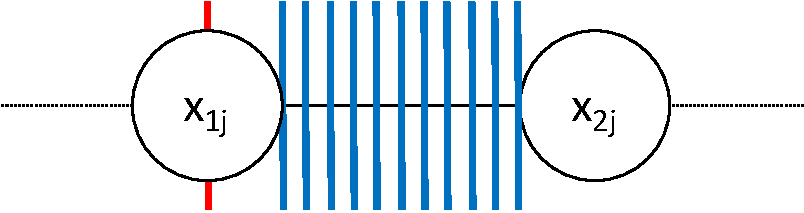
\includegraphics[scale=0.5]{figures/equivalent_thresholds.pdf}
	\end{center}
\end{frame}

\begin{frame}{A dynamic programming solution}
%	\begin{block}{Observation}
%	$\overset{\longleftarrow}{C_\tau}(\mu_1 \,|\, j, \delta)$ et $\overset{\longrightarrow}{C_\tau}(\mu_2 \,|\, j, \delta)$ calculent la somme d'un \red{ensemble de \emph{hinge loss}} de type:
%	\begin{itemize}
%		\item $\mu \mapsto \phi_\ell(-\mu + \ylower{i} + \epsilon)$ and $\mu \mapsto \phi_\ell(\mu - \yupper{i} + \epsilon)$
%	\end{itemize}
%	\end{block}
	\vspace{-3mm}

	\begin{equation*}
	\overset{\longleftarrow}{C_{\tau}}(\mu_1 \,|\, j, \delta) \ \eqdef \sum_{(\xb_i, \yb_i) \in S_{\tau}\,:\,x_{ij} \leq \delta} \phi_\ell(-\mu_1 + \ylower{i} + \epsilon) + \phi_\ell(\mu_1 - \yupper{i} + \epsilon) 
	\end{equation*}
	
	\begin{block}{Observation}
          Let $i_1,\dots,i_n$ be a permutation of $1,\dots,n$ such
          that $x_{i_1,\, j} \leq \cdots \leq x_{i_n,\, j}$ (sorted
          according to feature $j$).
\begin{eqnarray*}
  \overset{\longleftarrow}{C_{\tau}}(\mu_1 \,|\, j, \red{x_{i_n,\, j}}) \ & \eqdef & \sum_{(\xb_i, \yb_i) \in S_{\tau}\,:\,x_{ij} \,\leq\, x_{i_n,\, j}} \phi_\ell(-\mu_1 + \ylower{i} + \epsilon) + \phi_\ell(\mu_1 - \yupper{i} + \epsilon) \\
		&=& \overset{\longleftarrow}{C_{\tau}}(\mu_1 \,|\, j, \red{x_{i_{n-1},\, j}}) +  \phi_\ell(-\mu_1 + \ylower{n} + \epsilon) + \phi_\ell(\mu_1 - \yupper{n} + \epsilon)
		\end{eqnarray*}
	\end{block}
	
%	\pause
%	\vspace{3mm}
%	\begin{itemize}
%		\item<+-> Supposons qu'il existe un algorithme $\Omega$:
%			\begin{itemize}
%				\item \textbf{Entrée:} un \red{ensemble} quelconque de tels \red{\emph{hinge loss}} définis sur $\mu$
%				\vspace{1mm}
%				\item \textbf{Tâche:} calcule la somme de tous les hinge loss
%				\vspace{1mm}
%				\item \textbf{Sortie:} la valeur d'un minimum global et la valeur de $\mu$ correspondante
%			\end{itemize}
%		
%		\vspace{3mm}
%		\item<+-> Nous montrerons que nous pouvons utiliser un tel $\Omega$ pour résoudre le problème d'optimisation précédent de façon efficace
%	\end{itemize}
\end{frame}

%\begin{frame}{Vers une solution par programmation dynamique}
%	\begin{itemize}
%		\item<+-> Pour chaque valeur de seuil $\delta_{j,k}$, nous définissons $\Phi_{j,k}$, \red{l'ensemble des \emph{hinge loss}} de type $\mu \mapsto \phi_\ell(-\mu + \ylower{i} + \epsilon)$ et $\mu \mapsto \phi_\ell(\mu - \yupper{i} + \epsilon)$ pour les $(\xb_i, \yb_i) \in S_\tau$ tels que \red{$x_{ij} = \delta_{j,k}$}.
%		\vspace{3mm}
%		
%		\item<+-> Puisque $\delta_{j,i} < \delta_{j,i+1}$, nous avons:
%			\begin{equation*}
%			\min_\mu \overset{\longleftarrow}{C_{\tau}}(\mu \,|\, j, \delta_{j,k}) \,=\, \Omega(\Phi_{j,1} \cup \dots \cup \Phi_{j,k})
%			\end{equation*}
%			\begin{equation*}
%			\min_\mu \overset{\longrightarrow}{C_\tau}(\mu \,|\, j, \delta_{j,k}) \,=\, \Omega(\Phi_{j,k+1} \cup \dots \cup \Phi_{j,n_j})
%			\end{equation*}	
%		
%		\item<+->  De plus, nous pouvons obtenir $\overset{\longleftarrow}{C_\tau}(\mu \,|\, j, \delta_{j,k})$ à partir de $\overset{\longleftarrow}{C_\tau}(\mu \,|\, j, \delta_{j,k-1})$ en ajoutant les \emph{hinge loss} dans $\Phi_{j,k}$.
%		\vspace{3mm}
%		
%		\item<+-> De façon similaire, nous pouvons obtenir $\overset{\longrightarrow}{C_\tau}(\mu \,|\, j, \delta_{j,k})$ à partir de $\overset{\longrightarrow}{C_\tau}(\mu \,|\, j, \delta_{j,k-1})$ en enlevant les \emph{hinge loss} dans $\Phi_{j,k}$.
%	\end{itemize}
%\end{frame}
%
%\begin{frame}{Utilisation de l'algorithme $\Omega$}
%	Le coût associé à chacune des $n_j$ valeurs de seuil est donnée par:
%	\vspace{4mm}
%	\begin{equation*}\label{eq:dynprog}
%	\begin{array}{cccc}
%	\onslide<1>{\delta_{j,1}:} & \onslide<1,2>{\Omega(\Phi_{j,1})} & \onslide<1>{+} & \onslide<1,3->{\Omega(\Phi_{j,2} \cup \dots \cup \Phi_{j,n_j})} \\
%	\onslide<1>{\vdots} & \onslide<1-2>{\vdots} & & \onslide<1,3->{\vdots}\\
%	\onslide<1>{\delta_{j,i} :} & \onslide<1,2>{\Omega(\Phi_{j,1} \cup \dots \cup \Phi_{j,i})} & \onslide<1>{+} & \onslide<1,3->{\Omega(\Phi_{j,i+1} \cup \dots \cup \Phi_{j,n_j})} \\
%	\onslide<1>{\vdots} & \onslide<1,2>{\vdots} & & \onslide<1,3->{\vdots}\\
%	\onslide<1>{\delta_{j,n_j - 1} :} & \onslide<1-2>{\Omega(\Phi_{j,1} \cup \dots \cup \Phi_{j,n_j - 1})} & \onslide<1>{+} & \onslide<1,3->{\Omega(\Phi_{j,n_j})}
%	\end{array}
%	\end{equation*}
%	
%	\begin{center}
%		\only<1>{\vspace{0.6cm}Si $\Omega$ est un programme dynamique, nous pouvons calculer\\chaque solution efficacement}
%		\only<2>{\vspace{1cm}De \red{haut en bas} pour la \red{première colonne}}
%		\only<3>{\vspace{1cm}De \red{bas en haut} pour la \red{deuxième colonne}}
%	\end{center}
%\end{frame}

\begin{frame}{Minimizing a sum of hinge losses by dynamic programming}
	\only<1>{
		Both $\overset{\longleftarrow}{C_{\tau}}(\mu_1 \,|\, j, \delta_i)$ and $\overset{\longrightarrow}{C_{\tau}}(\mu_1 \,|\, j, \delta_i)$ are sums of \emph{hinge losses} of the following form (suppose $\ell(x) = x$): \vspace{4mm}
		\begin{itemize}
			\item Lower interval limit: $\mu \mapsto \phi_\ell(-\mu + \ylower{i} + \epsilon)$:
			\vspace{5mm}
			\begin{center}
				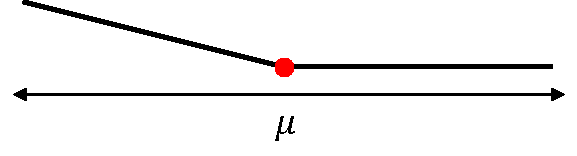
\includegraphics[scale=0.55]{figures/solver/lower_hinge.pdf}
			\end{center}
			\vspace{4mm}
			\item Upper interval limit: $\mu \mapsto \phi_\ell(\mu - \yupper{i} + \epsilon)$:
			\vspace{5mm}
			\begin{center}
				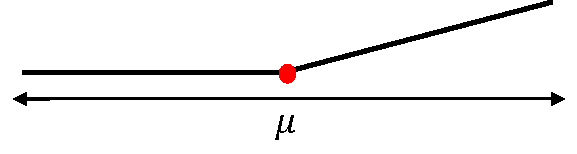
\includegraphics[scale=0.55]{figures/solver/upper_hinge.pdf}
			\end{center}
		\end{itemize}
	}
	\only<2>{\begin{center}
			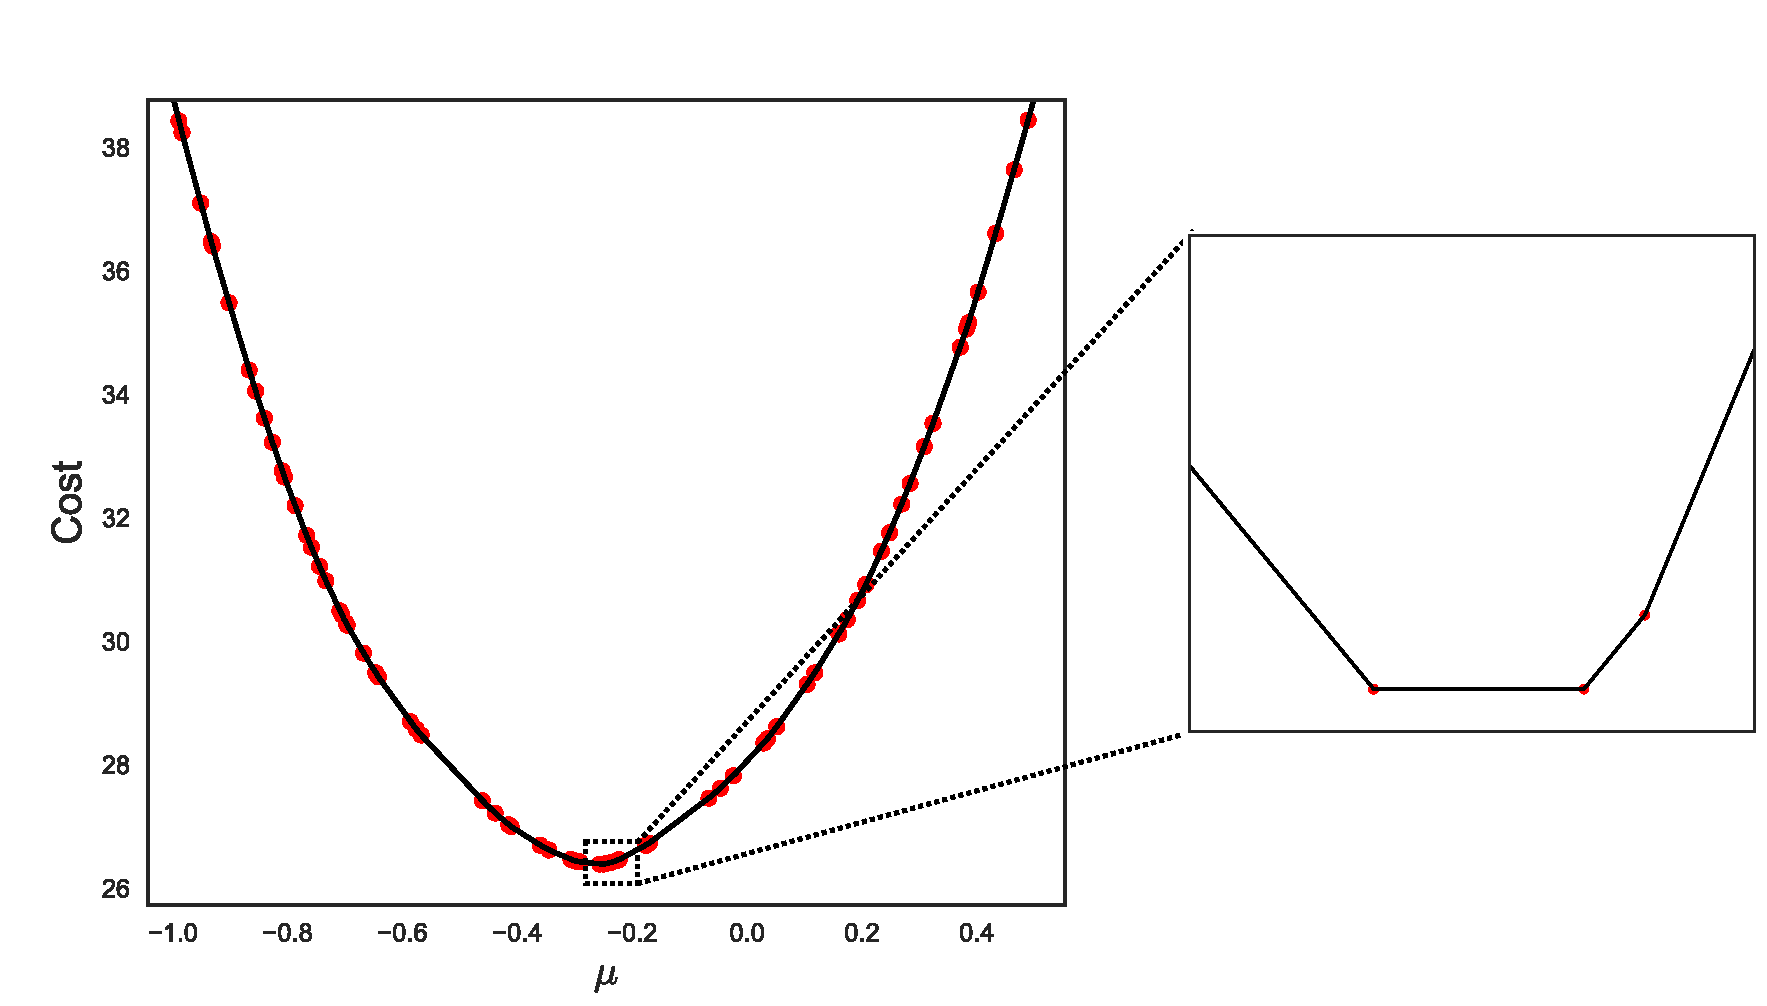
\includegraphics[scale=0.35]{figures/solver/sum_of_hinges.pdf}\\[3mm]
			A sum of \emph{hinge losses} is a \red{convex function} that is\\ \red{piecewise} linear (or quadratic)
		\end{center}
	}
	\only<3>{\begin{center}
			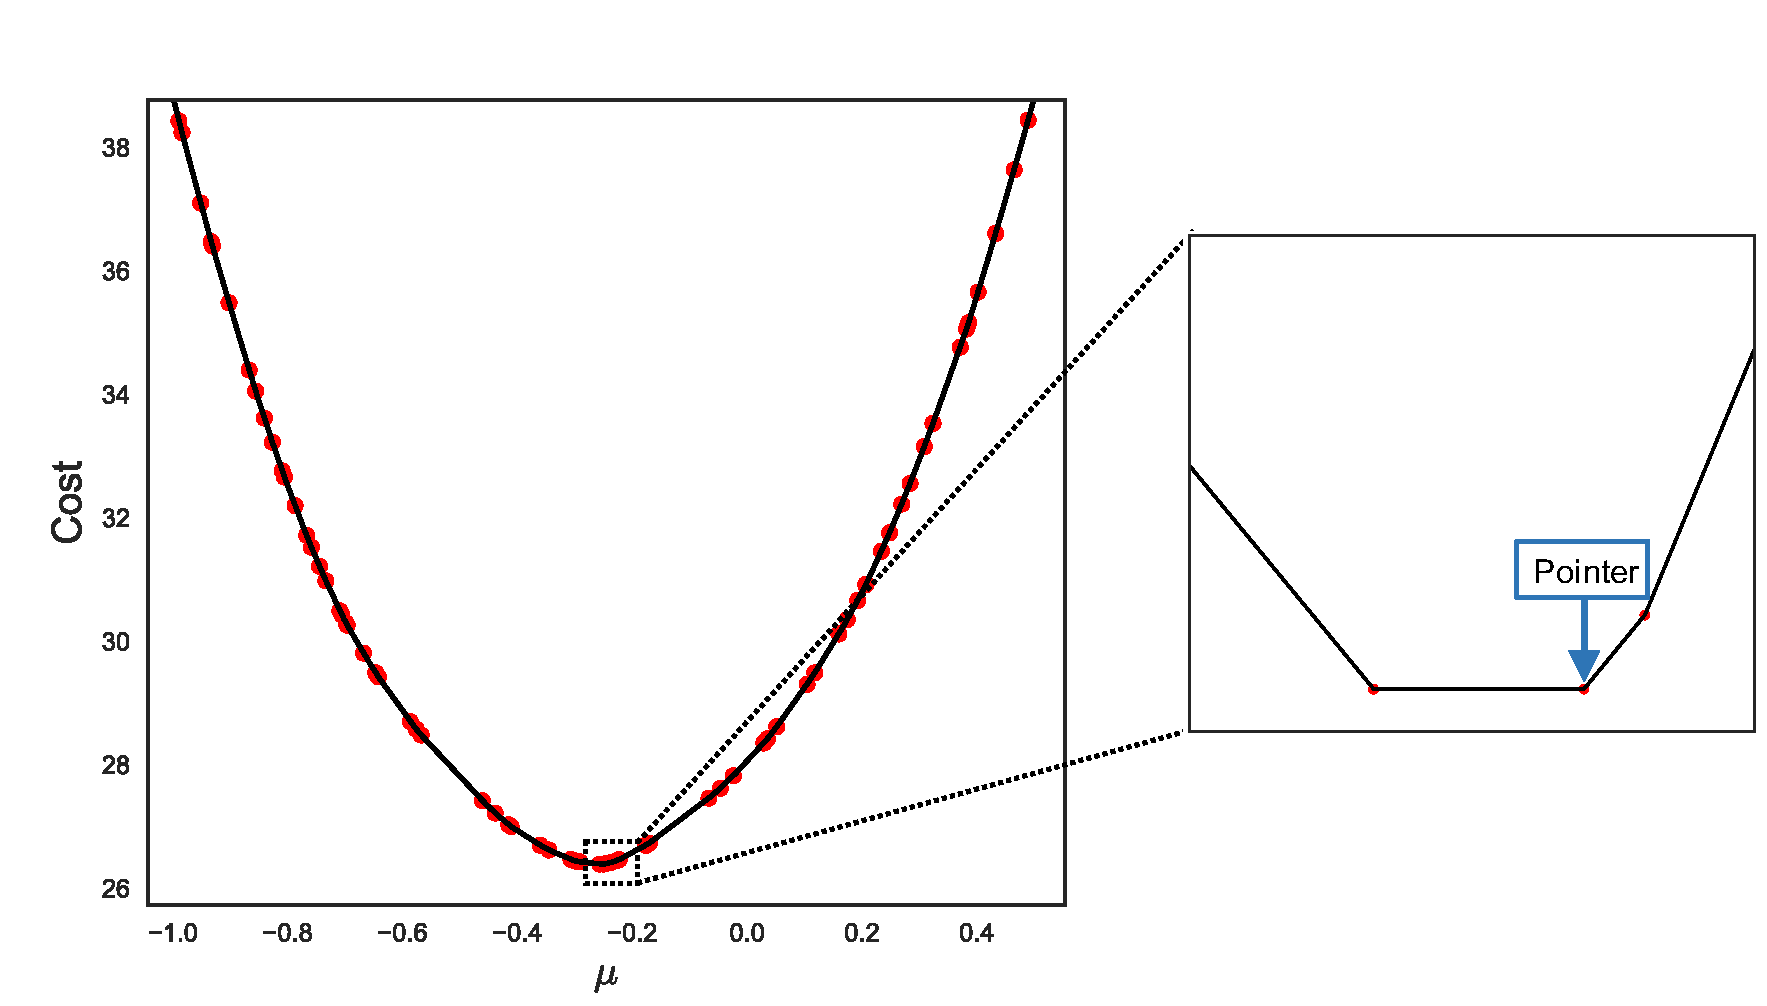
\includegraphics[scale=0.35]{figures/solver/sum_of_hinges_with_pointer.pdf}\\[3mm]
		     We maintain a \red{pointer} on the first changepoint that is\\ located to the \red{right of all global minima}
		\end{center}
	}
	\only<4>{\begin{center}
			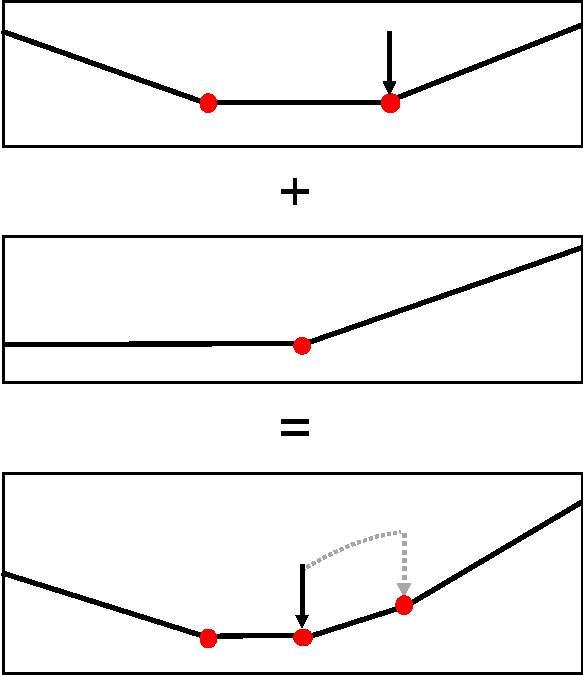
\includegraphics[scale=0.5]{figures/solver/pointer_needs_to_move.pdf}\\[3mm]
			The \emph{hinge losses} are added one by one.\\ Sometimes, the \red{pointer} must be \red{moved}.
		\end{center}
	}
\end{frame}

\begin{frame}{Moving the pointer}
  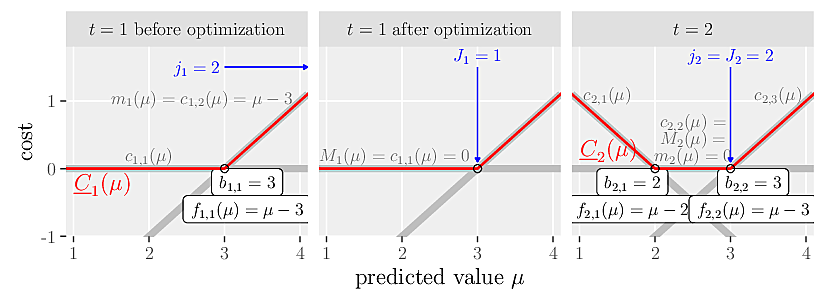
\includegraphics[width=\textwidth]{figure-algorithm-steps}

  \begin{itemize}
  \item Compute cost function pieces exactly in terms of coefficients.
  \item All the $c_{t,i}$ functions are not computed, that would be
    $O(n^2)$.
  \item Instead we compute just the minimum $m_t,M_t$ and
    the pointer $j_t,J_t$.
  \item Also need to store breakpoints $b_{t,i}$ and difference
    functions $f_{t,i}(\mu)=c_{t,i}(\mu)-c_{t,i-1}(\mu)$, C++STL map
    container, $O(\log n)$ insertion.
  \end{itemize}
\end{frame}

\begin{frame}{Time complexity of the dynamic programming algorithm}
	\begin{itemize}
		\item<+-> Suppose that we have $n$ \emph{hinge losses} \vspace{5mm}
		\item<+-> We add the \emph{hinge losses} to the sum one by one  ($n$ times) \vspace{5mm}
		\item<+-> The insertion of a new loss takes time $O(\max(\log n, k))$ where $k$ is the number of required pointer movements. \vspace{5mm}
		\item<+-> Case $\ell(x) = x$: we have shown that $k \in \{0, 1\}$, so $O(n \log n)$ \vspace{5mm}
		\item<+-> Case $\ell(x) = x^2$: we do not have a guarantee (empirical demonstration)
	\end{itemize}
\end{frame}

\begin{frame}{Learning a tree by minimizing over all features}
Overall time complexity per split $O(p n \log n)$

For example $p=4$ features in the figure below.

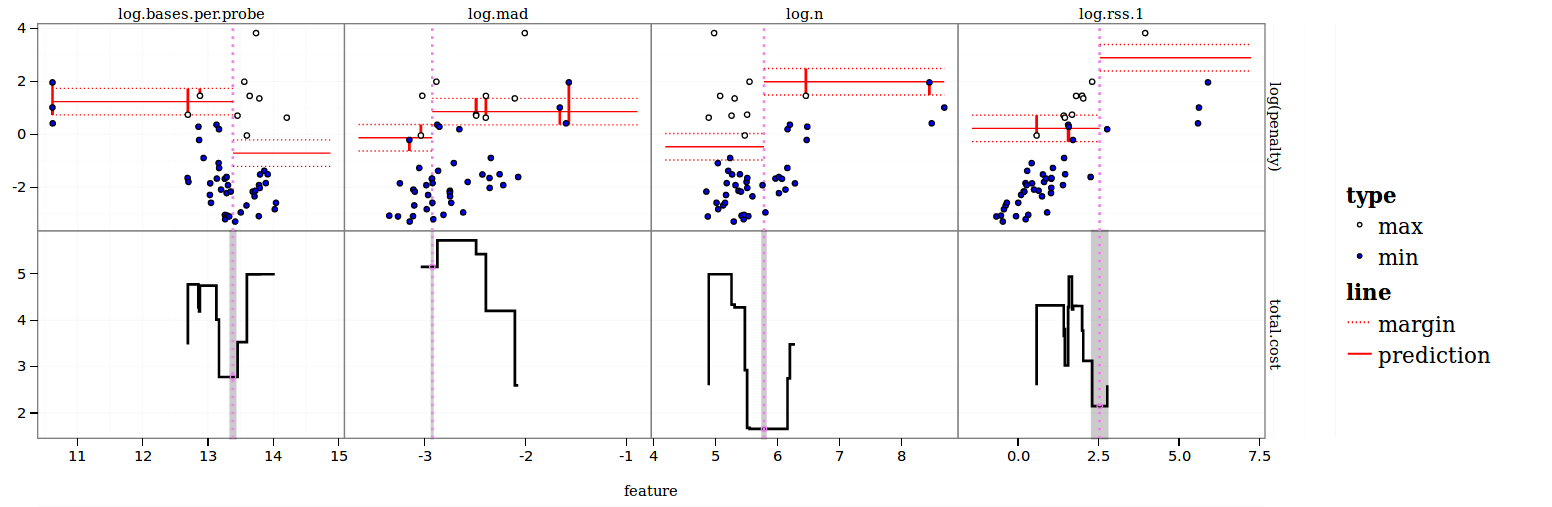
\includegraphics[width=\textwidth]{screenshot-search-over-features}

\small
\url{http://bl.ocks.org/tdhock/raw/105352ef496c22a80aea7c326b64c0a3/}

\end{frame}


\section{Results}


\begin{frame}{Empirical evaluation of time complexity}
	\begin{center}
		\begin{columns}
			\begin{column}{0.5\textwidth}
				\hspace*{3mm}
				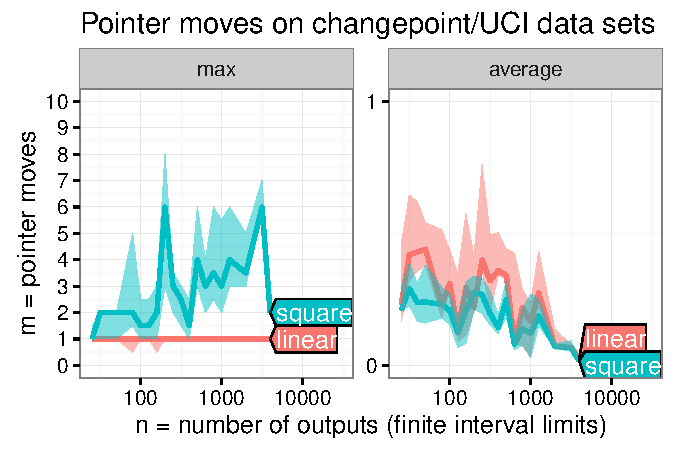
\includegraphics[height=1.6in]{figures/paper/figure-moves.pdf}
			\end{column}
			\begin{column}{0.5\textwidth}
				\hspace*{3mm}
				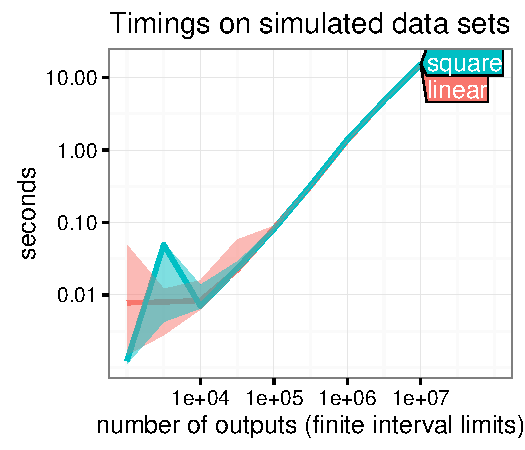
\includegraphics[height=1.6in]{figures/paper/figure-simulated-seconds.pdf}
			\end{column}
		\end{columns}
	\vspace{5mm}
	On average, we observed running times proportional to\\ \red{$n \log n$} for the \red{linear} and \red{quadratic} cases
	\end{center}
\end{frame}

\begin{frame}{MMIT can model non-linear functions}
	\begin{center}
		\resizebox{\textwidth}{!}{%% Creator: Matplotlib, PGF backend
%%
%% To include the figure in your LaTeX document, write
%%   \input{<filename>.pgf}
%%
%% Make sure the required packages are loaded in your preamble
%%   \usepackage{pgf}
%%
%% Figures using additional raster images can only be included by \input if
%% they are in the same directory as the main LaTeX file. For loading figures
%% from other directories you can use the `import` package
%%   \usepackage{import}
%% and then include the figures with
%%   \import{<path to file>}{<filename>.pgf}
%%
%% Matplotlib used the following preamble
%%   \usepackage[utf8x]{inputenc}
%%   \usepackage[T1]{fontenc}
%%
\begingroup%
\makeatletter%
\begin{pgfpicture}%
\pgfpathrectangle{\pgfpointorigin}{\pgfqpoint{5.625000in}{2.116587in}}%
\pgfusepath{use as bounding box, clip}%
\begin{pgfscope}%
\pgfsetbuttcap%
\pgfsetmiterjoin%
\definecolor{currentfill}{rgb}{1.000000,1.000000,1.000000}%
\pgfsetfillcolor{currentfill}%
\pgfsetlinewidth{0.000000pt}%
\definecolor{currentstroke}{rgb}{1.000000,1.000000,1.000000}%
\pgfsetstrokecolor{currentstroke}%
\pgfsetdash{}{0pt}%
\pgfpathmoveto{\pgfqpoint{0.000000in}{0.000000in}}%
\pgfpathlineto{\pgfqpoint{5.625000in}{0.000000in}}%
\pgfpathlineto{\pgfqpoint{5.625000in}{2.116587in}}%
\pgfpathlineto{\pgfqpoint{0.000000in}{2.116587in}}%
\pgfpathclose%
\pgfusepath{fill}%
\end{pgfscope}%
\begin{pgfscope}%
\pgfsetbuttcap%
\pgfsetmiterjoin%
\definecolor{currentfill}{rgb}{1.000000,1.000000,1.000000}%
\pgfsetfillcolor{currentfill}%
\pgfsetlinewidth{0.000000pt}%
\definecolor{currentstroke}{rgb}{0.000000,0.000000,0.000000}%
\pgfsetstrokecolor{currentstroke}%
\pgfsetstrokeopacity{0.000000}%
\pgfsetdash{}{0pt}%
\pgfpathmoveto{\pgfqpoint{0.100000in}{0.280143in}}%
\pgfpathlineto{\pgfqpoint{1.908333in}{0.280143in}}%
\pgfpathlineto{\pgfqpoint{1.908333in}{1.680143in}}%
\pgfpathlineto{\pgfqpoint{0.100000in}{1.680143in}}%
\pgfpathclose%
\pgfusepath{fill}%
\end{pgfscope}%
\begin{pgfscope}%
\definecolor{textcolor}{rgb}{0.150000,0.150000,0.150000}%
\pgfsetstrokecolor{textcolor}%
\pgfsetfillcolor{textcolor}%
\pgftext[x=1.004167in,y=0.210698in,,top]{\color{textcolor}\sffamily\fontsize{8.000000}{9.600000}\selectfont Signal feature (\(\displaystyle x\))}%
\end{pgfscope}%
\begin{pgfscope}%
\pgfpathrectangle{\pgfqpoint{0.100000in}{0.280143in}}{\pgfqpoint{1.808333in}{1.400000in}} %
\pgfusepath{clip}%
\pgfsetbuttcap%
\pgfsetroundjoin%
\definecolor{currentfill}{rgb}{0.501961,0.501961,0.501961}%
\pgfsetfillcolor{currentfill}%
\pgfsetfillopacity{0.500000}%
\pgfsetlinewidth{1.003750pt}%
\definecolor{currentstroke}{rgb}{0.501961,0.501961,0.501961}%
\pgfsetstrokecolor{currentstroke}%
\pgfsetstrokeopacity{0.500000}%
\pgfsetdash{}{0pt}%
\pgfpathmoveto{\pgfqpoint{0.789873in}{0.783824in}}%
\pgfpathcurveto{\pgfqpoint{0.795697in}{0.783824in}}{\pgfqpoint{0.801283in}{0.786138in}}{\pgfqpoint{0.805401in}{0.790256in}}%
\pgfpathcurveto{\pgfqpoint{0.809520in}{0.794374in}}{\pgfqpoint{0.811833in}{0.799961in}}{\pgfqpoint{0.811833in}{0.805785in}}%
\pgfpathcurveto{\pgfqpoint{0.811833in}{0.811609in}}{\pgfqpoint{0.809520in}{0.817195in}}{\pgfqpoint{0.805401in}{0.821313in}}%
\pgfpathcurveto{\pgfqpoint{0.801283in}{0.825431in}}{\pgfqpoint{0.795697in}{0.827745in}}{\pgfqpoint{0.789873in}{0.827745in}}%
\pgfpathcurveto{\pgfqpoint{0.784049in}{0.827745in}}{\pgfqpoint{0.778463in}{0.825431in}}{\pgfqpoint{0.774345in}{0.821313in}}%
\pgfpathcurveto{\pgfqpoint{0.770227in}{0.817195in}}{\pgfqpoint{0.767913in}{0.811609in}}{\pgfqpoint{0.767913in}{0.805785in}}%
\pgfpathcurveto{\pgfqpoint{0.767913in}{0.799961in}}{\pgfqpoint{0.770227in}{0.794374in}}{\pgfqpoint{0.774345in}{0.790256in}}%
\pgfpathcurveto{\pgfqpoint{0.778463in}{0.786138in}}{\pgfqpoint{0.784049in}{0.783824in}}{\pgfqpoint{0.789873in}{0.783824in}}%
\pgfpathclose%
\pgfusepath{stroke,fill}%
\end{pgfscope}%
\begin{pgfscope}%
\pgfpathrectangle{\pgfqpoint{0.100000in}{0.280143in}}{\pgfqpoint{1.808333in}{1.400000in}} %
\pgfusepath{clip}%
\pgfsetbuttcap%
\pgfsetroundjoin%
\definecolor{currentfill}{rgb}{0.501961,0.501961,0.501961}%
\pgfsetfillcolor{currentfill}%
\pgfsetfillopacity{0.500000}%
\pgfsetlinewidth{1.003750pt}%
\definecolor{currentstroke}{rgb}{0.501961,0.501961,0.501961}%
\pgfsetstrokecolor{currentstroke}%
\pgfsetstrokeopacity{0.500000}%
\pgfsetdash{}{0pt}%
\pgfpathmoveto{\pgfqpoint{1.186439in}{0.684963in}}%
\pgfpathcurveto{\pgfqpoint{1.192263in}{0.684963in}}{\pgfqpoint{1.197849in}{0.687277in}}{\pgfqpoint{1.201967in}{0.691395in}}%
\pgfpathcurveto{\pgfqpoint{1.206086in}{0.695513in}}{\pgfqpoint{1.208399in}{0.701099in}}{\pgfqpoint{1.208399in}{0.706923in}}%
\pgfpathcurveto{\pgfqpoint{1.208399in}{0.712747in}}{\pgfqpoint{1.206086in}{0.718333in}}{\pgfqpoint{1.201967in}{0.722452in}}%
\pgfpathcurveto{\pgfqpoint{1.197849in}{0.726570in}}{\pgfqpoint{1.192263in}{0.728884in}}{\pgfqpoint{1.186439in}{0.728884in}}%
\pgfpathcurveto{\pgfqpoint{1.180615in}{0.728884in}}{\pgfqpoint{1.175029in}{0.726570in}}{\pgfqpoint{1.170911in}{0.722452in}}%
\pgfpathcurveto{\pgfqpoint{1.166793in}{0.718333in}}{\pgfqpoint{1.164479in}{0.712747in}}{\pgfqpoint{1.164479in}{0.706923in}}%
\pgfpathcurveto{\pgfqpoint{1.164479in}{0.701099in}}{\pgfqpoint{1.166793in}{0.695513in}}{\pgfqpoint{1.170911in}{0.691395in}}%
\pgfpathcurveto{\pgfqpoint{1.175029in}{0.687277in}}{\pgfqpoint{1.180615in}{0.684963in}}{\pgfqpoint{1.186439in}{0.684963in}}%
\pgfpathclose%
\pgfusepath{stroke,fill}%
\end{pgfscope}%
\begin{pgfscope}%
\pgfpathrectangle{\pgfqpoint{0.100000in}{0.280143in}}{\pgfqpoint{1.808333in}{1.400000in}} %
\pgfusepath{clip}%
\pgfsetbuttcap%
\pgfsetroundjoin%
\definecolor{currentfill}{rgb}{0.501961,0.501961,0.501961}%
\pgfsetfillcolor{currentfill}%
\pgfsetfillopacity{0.500000}%
\pgfsetlinewidth{1.003750pt}%
\definecolor{currentstroke}{rgb}{0.501961,0.501961,0.501961}%
\pgfsetstrokecolor{currentstroke}%
\pgfsetstrokeopacity{0.500000}%
\pgfsetdash{}{0pt}%
\pgfpathmoveto{\pgfqpoint{0.367925in}{1.315695in}}%
\pgfpathcurveto{\pgfqpoint{0.373749in}{1.315695in}}{\pgfqpoint{0.379335in}{1.318008in}}{\pgfqpoint{0.383453in}{1.322127in}}%
\pgfpathcurveto{\pgfqpoint{0.387572in}{1.326245in}}{\pgfqpoint{0.389885in}{1.331831in}}{\pgfqpoint{0.389885in}{1.337655in}}%
\pgfpathcurveto{\pgfqpoint{0.389885in}{1.343479in}}{\pgfqpoint{0.387572in}{1.349065in}}{\pgfqpoint{0.383453in}{1.353183in}}%
\pgfpathcurveto{\pgfqpoint{0.379335in}{1.357301in}}{\pgfqpoint{0.373749in}{1.359615in}}{\pgfqpoint{0.367925in}{1.359615in}}%
\pgfpathcurveto{\pgfqpoint{0.362101in}{1.359615in}}{\pgfqpoint{0.356515in}{1.357301in}}{\pgfqpoint{0.352397in}{1.353183in}}%
\pgfpathcurveto{\pgfqpoint{0.348279in}{1.349065in}}{\pgfqpoint{0.345965in}{1.343479in}}{\pgfqpoint{0.345965in}{1.337655in}}%
\pgfpathcurveto{\pgfqpoint{0.345965in}{1.331831in}}{\pgfqpoint{0.348279in}{1.326245in}}{\pgfqpoint{0.352397in}{1.322127in}}%
\pgfpathcurveto{\pgfqpoint{0.356515in}{1.318008in}}{\pgfqpoint{0.362101in}{1.315695in}}{\pgfqpoint{0.367925in}{1.315695in}}%
\pgfpathclose%
\pgfusepath{stroke,fill}%
\end{pgfscope}%
\begin{pgfscope}%
\pgfpathrectangle{\pgfqpoint{0.100000in}{0.280143in}}{\pgfqpoint{1.808333in}{1.400000in}} %
\pgfusepath{clip}%
\pgfsetbuttcap%
\pgfsetroundjoin%
\definecolor{currentfill}{rgb}{0.501961,0.501961,0.501961}%
\pgfsetfillcolor{currentfill}%
\pgfsetfillopacity{0.500000}%
\pgfsetlinewidth{1.003750pt}%
\definecolor{currentstroke}{rgb}{0.501961,0.501961,0.501961}%
\pgfsetstrokecolor{currentstroke}%
\pgfsetstrokeopacity{0.500000}%
\pgfsetdash{}{0pt}%
\pgfpathmoveto{\pgfqpoint{0.813497in}{0.831509in}}%
\pgfpathcurveto{\pgfqpoint{0.819321in}{0.831509in}}{\pgfqpoint{0.824907in}{0.833823in}}{\pgfqpoint{0.829026in}{0.837941in}}%
\pgfpathcurveto{\pgfqpoint{0.833144in}{0.842059in}}{\pgfqpoint{0.835458in}{0.847645in}}{\pgfqpoint{0.835458in}{0.853469in}}%
\pgfpathcurveto{\pgfqpoint{0.835458in}{0.859293in}}{\pgfqpoint{0.833144in}{0.864879in}}{\pgfqpoint{0.829026in}{0.868997in}}%
\pgfpathcurveto{\pgfqpoint{0.824907in}{0.873115in}}{\pgfqpoint{0.819321in}{0.875429in}}{\pgfqpoint{0.813497in}{0.875429in}}%
\pgfpathcurveto{\pgfqpoint{0.807673in}{0.875429in}}{\pgfqpoint{0.802087in}{0.873115in}}{\pgfqpoint{0.797969in}{0.868997in}}%
\pgfpathcurveto{\pgfqpoint{0.793851in}{0.864879in}}{\pgfqpoint{0.791537in}{0.859293in}}{\pgfqpoint{0.791537in}{0.853469in}}%
\pgfpathcurveto{\pgfqpoint{0.791537in}{0.847645in}}{\pgfqpoint{0.793851in}{0.842059in}}{\pgfqpoint{0.797969in}{0.837941in}}%
\pgfpathcurveto{\pgfqpoint{0.802087in}{0.833823in}}{\pgfqpoint{0.807673in}{0.831509in}}{\pgfqpoint{0.813497in}{0.831509in}}%
\pgfpathclose%
\pgfusepath{stroke,fill}%
\end{pgfscope}%
\begin{pgfscope}%
\pgfpathrectangle{\pgfqpoint{0.100000in}{0.280143in}}{\pgfqpoint{1.808333in}{1.400000in}} %
\pgfusepath{clip}%
\pgfsetbuttcap%
\pgfsetroundjoin%
\definecolor{currentfill}{rgb}{0.501961,0.501961,0.501961}%
\pgfsetfillcolor{currentfill}%
\pgfsetfillopacity{0.500000}%
\pgfsetlinewidth{1.003750pt}%
\definecolor{currentstroke}{rgb}{0.501961,0.501961,0.501961}%
\pgfsetstrokecolor{currentstroke}%
\pgfsetstrokeopacity{0.500000}%
\pgfsetdash{}{0pt}%
\pgfpathmoveto{\pgfqpoint{1.606296in}{1.290357in}}%
\pgfpathcurveto{\pgfqpoint{1.612120in}{1.290357in}}{\pgfqpoint{1.617706in}{1.292671in}}{\pgfqpoint{1.621824in}{1.296789in}}%
\pgfpathcurveto{\pgfqpoint{1.625942in}{1.300907in}}{\pgfqpoint{1.628256in}{1.306493in}}{\pgfqpoint{1.628256in}{1.312317in}}%
\pgfpathcurveto{\pgfqpoint{1.628256in}{1.318141in}}{\pgfqpoint{1.625942in}{1.323728in}}{\pgfqpoint{1.621824in}{1.327846in}}%
\pgfpathcurveto{\pgfqpoint{1.617706in}{1.331964in}}{\pgfqpoint{1.612120in}{1.334278in}}{\pgfqpoint{1.606296in}{1.334278in}}%
\pgfpathcurveto{\pgfqpoint{1.600472in}{1.334278in}}{\pgfqpoint{1.594886in}{1.331964in}}{\pgfqpoint{1.590768in}{1.327846in}}%
\pgfpathcurveto{\pgfqpoint{1.586650in}{1.323728in}}{\pgfqpoint{1.584336in}{1.318141in}}{\pgfqpoint{1.584336in}{1.312317in}}%
\pgfpathcurveto{\pgfqpoint{1.584336in}{1.306493in}}{\pgfqpoint{1.586650in}{1.300907in}}{\pgfqpoint{1.590768in}{1.296789in}}%
\pgfpathcurveto{\pgfqpoint{1.594886in}{1.292671in}}{\pgfqpoint{1.600472in}{1.290357in}}{\pgfqpoint{1.606296in}{1.290357in}}%
\pgfpathclose%
\pgfusepath{stroke,fill}%
\end{pgfscope}%
\begin{pgfscope}%
\pgfpathrectangle{\pgfqpoint{0.100000in}{0.280143in}}{\pgfqpoint{1.808333in}{1.400000in}} %
\pgfusepath{clip}%
\pgfsetbuttcap%
\pgfsetroundjoin%
\definecolor{currentfill}{rgb}{0.501961,0.501961,0.501961}%
\pgfsetfillcolor{currentfill}%
\pgfsetfillopacity{0.500000}%
\pgfsetlinewidth{1.003750pt}%
\definecolor{currentstroke}{rgb}{0.501961,0.501961,0.501961}%
\pgfsetstrokecolor{currentstroke}%
\pgfsetstrokeopacity{0.500000}%
\pgfsetdash{}{0pt}%
\pgfpathmoveto{\pgfqpoint{0.216511in}{1.483245in}}%
\pgfpathcurveto{\pgfqpoint{0.222335in}{1.483245in}}{\pgfqpoint{0.227921in}{1.485558in}}{\pgfqpoint{0.232039in}{1.489677in}}%
\pgfpathcurveto{\pgfqpoint{0.236158in}{1.493795in}}{\pgfqpoint{0.238471in}{1.499381in}}{\pgfqpoint{0.238471in}{1.505205in}}%
\pgfpathcurveto{\pgfqpoint{0.238471in}{1.511029in}}{\pgfqpoint{0.236158in}{1.516615in}}{\pgfqpoint{0.232039in}{1.520733in}}%
\pgfpathcurveto{\pgfqpoint{0.227921in}{1.524851in}}{\pgfqpoint{0.222335in}{1.527165in}}{\pgfqpoint{0.216511in}{1.527165in}}%
\pgfpathcurveto{\pgfqpoint{0.210687in}{1.527165in}}{\pgfqpoint{0.205101in}{1.524851in}}{\pgfqpoint{0.200983in}{1.520733in}}%
\pgfpathcurveto{\pgfqpoint{0.196865in}{1.516615in}}{\pgfqpoint{0.194551in}{1.511029in}}{\pgfqpoint{0.194551in}{1.505205in}}%
\pgfpathcurveto{\pgfqpoint{0.194551in}{1.499381in}}{\pgfqpoint{0.196865in}{1.493795in}}{\pgfqpoint{0.200983in}{1.489677in}}%
\pgfpathcurveto{\pgfqpoint{0.205101in}{1.485558in}}{\pgfqpoint{0.210687in}{1.483245in}}{\pgfqpoint{0.216511in}{1.483245in}}%
\pgfpathclose%
\pgfusepath{stroke,fill}%
\end{pgfscope}%
\begin{pgfscope}%
\pgfpathrectangle{\pgfqpoint{0.100000in}{0.280143in}}{\pgfqpoint{1.808333in}{1.400000in}} %
\pgfusepath{clip}%
\pgfsetbuttcap%
\pgfsetroundjoin%
\definecolor{currentfill}{rgb}{0.501961,0.501961,0.501961}%
\pgfsetfillcolor{currentfill}%
\pgfsetfillopacity{0.500000}%
\pgfsetlinewidth{1.003750pt}%
\definecolor{currentstroke}{rgb}{0.501961,0.501961,0.501961}%
\pgfsetstrokecolor{currentstroke}%
\pgfsetstrokeopacity{0.500000}%
\pgfsetdash{}{0pt}%
\pgfpathmoveto{\pgfqpoint{1.772307in}{1.493402in}}%
\pgfpathcurveto{\pgfqpoint{1.778130in}{1.493402in}}{\pgfqpoint{1.783717in}{1.495716in}}{\pgfqpoint{1.787835in}{1.499834in}}%
\pgfpathcurveto{\pgfqpoint{1.791953in}{1.503952in}}{\pgfqpoint{1.794267in}{1.509538in}}{\pgfqpoint{1.794267in}{1.515362in}}%
\pgfpathcurveto{\pgfqpoint{1.794267in}{1.521186in}}{\pgfqpoint{1.791953in}{1.526772in}}{\pgfqpoint{1.787835in}{1.530890in}}%
\pgfpathcurveto{\pgfqpoint{1.783717in}{1.535009in}}{\pgfqpoint{1.778130in}{1.537322in}}{\pgfqpoint{1.772307in}{1.537322in}}%
\pgfpathcurveto{\pgfqpoint{1.766483in}{1.537322in}}{\pgfqpoint{1.760896in}{1.535009in}}{\pgfqpoint{1.756778in}{1.530890in}}%
\pgfpathcurveto{\pgfqpoint{1.752660in}{1.526772in}}{\pgfqpoint{1.750346in}{1.521186in}}{\pgfqpoint{1.750346in}{1.515362in}}%
\pgfpathcurveto{\pgfqpoint{1.750346in}{1.509538in}}{\pgfqpoint{1.752660in}{1.503952in}}{\pgfqpoint{1.756778in}{1.499834in}}%
\pgfpathcurveto{\pgfqpoint{1.760896in}{1.495716in}}{\pgfqpoint{1.766483in}{1.493402in}}{\pgfqpoint{1.772307in}{1.493402in}}%
\pgfpathclose%
\pgfusepath{stroke,fill}%
\end{pgfscope}%
\begin{pgfscope}%
\pgfpathrectangle{\pgfqpoint{0.100000in}{0.280143in}}{\pgfqpoint{1.808333in}{1.400000in}} %
\pgfusepath{clip}%
\pgfsetbuttcap%
\pgfsetroundjoin%
\definecolor{currentfill}{rgb}{0.501961,0.501961,0.501961}%
\pgfsetfillcolor{currentfill}%
\pgfsetfillopacity{0.500000}%
\pgfsetlinewidth{1.003750pt}%
\definecolor{currentstroke}{rgb}{0.501961,0.501961,0.501961}%
\pgfsetstrokecolor{currentstroke}%
\pgfsetstrokeopacity{0.500000}%
\pgfsetdash{}{0pt}%
\pgfpathmoveto{\pgfqpoint{0.778582in}{0.879844in}}%
\pgfpathcurveto{\pgfqpoint{0.784406in}{0.879844in}}{\pgfqpoint{0.789992in}{0.882158in}}{\pgfqpoint{0.794110in}{0.886276in}}%
\pgfpathcurveto{\pgfqpoint{0.798228in}{0.890394in}}{\pgfqpoint{0.800542in}{0.895981in}}{\pgfqpoint{0.800542in}{0.901805in}}%
\pgfpathcurveto{\pgfqpoint{0.800542in}{0.907628in}}{\pgfqpoint{0.798228in}{0.913215in}}{\pgfqpoint{0.794110in}{0.917333in}}%
\pgfpathcurveto{\pgfqpoint{0.789992in}{0.921451in}}{\pgfqpoint{0.784406in}{0.923765in}}{\pgfqpoint{0.778582in}{0.923765in}}%
\pgfpathcurveto{\pgfqpoint{0.772758in}{0.923765in}}{\pgfqpoint{0.767172in}{0.921451in}}{\pgfqpoint{0.763054in}{0.917333in}}%
\pgfpathcurveto{\pgfqpoint{0.758935in}{0.913215in}}{\pgfqpoint{0.756622in}{0.907628in}}{\pgfqpoint{0.756622in}{0.901805in}}%
\pgfpathcurveto{\pgfqpoint{0.756622in}{0.895981in}}{\pgfqpoint{0.758935in}{0.890394in}}{\pgfqpoint{0.763054in}{0.886276in}}%
\pgfpathcurveto{\pgfqpoint{0.767172in}{0.882158in}}{\pgfqpoint{0.772758in}{0.879844in}}{\pgfqpoint{0.778582in}{0.879844in}}%
\pgfpathclose%
\pgfusepath{stroke,fill}%
\end{pgfscope}%
\begin{pgfscope}%
\pgfpathrectangle{\pgfqpoint{0.100000in}{0.280143in}}{\pgfqpoint{1.808333in}{1.400000in}} %
\pgfusepath{clip}%
\pgfsetbuttcap%
\pgfsetroundjoin%
\definecolor{currentfill}{rgb}{0.501961,0.501961,0.501961}%
\pgfsetfillcolor{currentfill}%
\pgfsetfillopacity{0.500000}%
\pgfsetlinewidth{1.003750pt}%
\definecolor{currentstroke}{rgb}{0.501961,0.501961,0.501961}%
\pgfsetstrokecolor{currentstroke}%
\pgfsetstrokeopacity{0.500000}%
\pgfsetdash{}{0pt}%
\pgfpathmoveto{\pgfqpoint{0.733936in}{0.853402in}}%
\pgfpathcurveto{\pgfqpoint{0.739760in}{0.853402in}}{\pgfqpoint{0.745346in}{0.855716in}}{\pgfqpoint{0.749464in}{0.859834in}}%
\pgfpathcurveto{\pgfqpoint{0.753583in}{0.863952in}}{\pgfqpoint{0.755896in}{0.869538in}}{\pgfqpoint{0.755896in}{0.875362in}}%
\pgfpathcurveto{\pgfqpoint{0.755896in}{0.881186in}}{\pgfqpoint{0.753583in}{0.886772in}}{\pgfqpoint{0.749464in}{0.890890in}}%
\pgfpathcurveto{\pgfqpoint{0.745346in}{0.895009in}}{\pgfqpoint{0.739760in}{0.897322in}}{\pgfqpoint{0.733936in}{0.897322in}}%
\pgfpathcurveto{\pgfqpoint{0.728112in}{0.897322in}}{\pgfqpoint{0.722526in}{0.895009in}}{\pgfqpoint{0.718408in}{0.890890in}}%
\pgfpathcurveto{\pgfqpoint{0.714290in}{0.886772in}}{\pgfqpoint{0.711976in}{0.881186in}}{\pgfqpoint{0.711976in}{0.875362in}}%
\pgfpathcurveto{\pgfqpoint{0.711976in}{0.869538in}}{\pgfqpoint{0.714290in}{0.863952in}}{\pgfqpoint{0.718408in}{0.859834in}}%
\pgfpathcurveto{\pgfqpoint{0.722526in}{0.855716in}}{\pgfqpoint{0.728112in}{0.853402in}}{\pgfqpoint{0.733936in}{0.853402in}}%
\pgfpathclose%
\pgfusepath{stroke,fill}%
\end{pgfscope}%
\begin{pgfscope}%
\pgfpathrectangle{\pgfqpoint{0.100000in}{0.280143in}}{\pgfqpoint{1.808333in}{1.400000in}} %
\pgfusepath{clip}%
\pgfsetbuttcap%
\pgfsetroundjoin%
\definecolor{currentfill}{rgb}{0.501961,0.501961,0.501961}%
\pgfsetfillcolor{currentfill}%
\pgfsetfillopacity{0.500000}%
\pgfsetlinewidth{1.003750pt}%
\definecolor{currentstroke}{rgb}{0.501961,0.501961,0.501961}%
\pgfsetstrokecolor{currentstroke}%
\pgfsetstrokeopacity{0.500000}%
\pgfsetdash{}{0pt}%
\pgfpathmoveto{\pgfqpoint{1.236870in}{0.956194in}}%
\pgfpathcurveto{\pgfqpoint{1.242694in}{0.956194in}}{\pgfqpoint{1.248280in}{0.958508in}}{\pgfqpoint{1.252398in}{0.962626in}}%
\pgfpathcurveto{\pgfqpoint{1.256516in}{0.966744in}}{\pgfqpoint{1.258830in}{0.972330in}}{\pgfqpoint{1.258830in}{0.978154in}}%
\pgfpathcurveto{\pgfqpoint{1.258830in}{0.983978in}}{\pgfqpoint{1.256516in}{0.989564in}}{\pgfqpoint{1.252398in}{0.993683in}}%
\pgfpathcurveto{\pgfqpoint{1.248280in}{0.997801in}}{\pgfqpoint{1.242694in}{1.000115in}}{\pgfqpoint{1.236870in}{1.000115in}}%
\pgfpathcurveto{\pgfqpoint{1.231046in}{1.000115in}}{\pgfqpoint{1.225460in}{0.997801in}}{\pgfqpoint{1.221342in}{0.993683in}}%
\pgfpathcurveto{\pgfqpoint{1.217224in}{0.989564in}}{\pgfqpoint{1.214910in}{0.983978in}}{\pgfqpoint{1.214910in}{0.978154in}}%
\pgfpathcurveto{\pgfqpoint{1.214910in}{0.972330in}}{\pgfqpoint{1.217224in}{0.966744in}}{\pgfqpoint{1.221342in}{0.962626in}}%
\pgfpathcurveto{\pgfqpoint{1.225460in}{0.958508in}}{\pgfqpoint{1.231046in}{0.956194in}}{\pgfqpoint{1.236870in}{0.956194in}}%
\pgfpathclose%
\pgfusepath{stroke,fill}%
\end{pgfscope}%
\begin{pgfscope}%
\pgfpathrectangle{\pgfqpoint{0.100000in}{0.280143in}}{\pgfqpoint{1.808333in}{1.400000in}} %
\pgfusepath{clip}%
\pgfsetbuttcap%
\pgfsetroundjoin%
\definecolor{currentfill}{rgb}{0.501961,0.501961,0.501961}%
\pgfsetfillcolor{currentfill}%
\pgfsetfillopacity{0.500000}%
\pgfsetlinewidth{1.003750pt}%
\definecolor{currentstroke}{rgb}{0.501961,0.501961,0.501961}%
\pgfsetstrokecolor{currentstroke}%
\pgfsetstrokeopacity{0.500000}%
\pgfsetdash{}{0pt}%
\pgfpathmoveto{\pgfqpoint{1.262907in}{0.813085in}}%
\pgfpathcurveto{\pgfqpoint{1.268731in}{0.813085in}}{\pgfqpoint{1.274317in}{0.815399in}}{\pgfqpoint{1.278436in}{0.819517in}}%
\pgfpathcurveto{\pgfqpoint{1.282554in}{0.823635in}}{\pgfqpoint{1.284868in}{0.829221in}}{\pgfqpoint{1.284868in}{0.835045in}}%
\pgfpathcurveto{\pgfqpoint{1.284868in}{0.840869in}}{\pgfqpoint{1.282554in}{0.846455in}}{\pgfqpoint{1.278436in}{0.850573in}}%
\pgfpathcurveto{\pgfqpoint{1.274317in}{0.854691in}}{\pgfqpoint{1.268731in}{0.857005in}}{\pgfqpoint{1.262907in}{0.857005in}}%
\pgfpathcurveto{\pgfqpoint{1.257083in}{0.857005in}}{\pgfqpoint{1.251497in}{0.854691in}}{\pgfqpoint{1.247379in}{0.850573in}}%
\pgfpathcurveto{\pgfqpoint{1.243261in}{0.846455in}}{\pgfqpoint{1.240947in}{0.840869in}}{\pgfqpoint{1.240947in}{0.835045in}}%
\pgfpathcurveto{\pgfqpoint{1.240947in}{0.829221in}}{\pgfqpoint{1.243261in}{0.823635in}}{\pgfqpoint{1.247379in}{0.819517in}}%
\pgfpathcurveto{\pgfqpoint{1.251497in}{0.815399in}}{\pgfqpoint{1.257083in}{0.813085in}}{\pgfqpoint{1.262907in}{0.813085in}}%
\pgfpathclose%
\pgfusepath{stroke,fill}%
\end{pgfscope}%
\begin{pgfscope}%
\pgfpathrectangle{\pgfqpoint{0.100000in}{0.280143in}}{\pgfqpoint{1.808333in}{1.400000in}} %
\pgfusepath{clip}%
\pgfsetbuttcap%
\pgfsetroundjoin%
\definecolor{currentfill}{rgb}{0.501961,0.501961,0.501961}%
\pgfsetfillcolor{currentfill}%
\pgfsetfillopacity{0.500000}%
\pgfsetlinewidth{1.003750pt}%
\definecolor{currentstroke}{rgb}{0.501961,0.501961,0.501961}%
\pgfsetstrokecolor{currentstroke}%
\pgfsetstrokeopacity{0.500000}%
\pgfsetdash{}{0pt}%
\pgfpathmoveto{\pgfqpoint{1.735562in}{1.414067in}}%
\pgfpathcurveto{\pgfqpoint{1.741386in}{1.414067in}}{\pgfqpoint{1.746972in}{1.416381in}}{\pgfqpoint{1.751090in}{1.420499in}}%
\pgfpathcurveto{\pgfqpoint{1.755208in}{1.424617in}}{\pgfqpoint{1.757522in}{1.430203in}}{\pgfqpoint{1.757522in}{1.436027in}}%
\pgfpathcurveto{\pgfqpoint{1.757522in}{1.441851in}}{\pgfqpoint{1.755208in}{1.447437in}}{\pgfqpoint{1.751090in}{1.451555in}}%
\pgfpathcurveto{\pgfqpoint{1.746972in}{1.455673in}}{\pgfqpoint{1.741386in}{1.457987in}}{\pgfqpoint{1.735562in}{1.457987in}}%
\pgfpathcurveto{\pgfqpoint{1.729738in}{1.457987in}}{\pgfqpoint{1.724152in}{1.455673in}}{\pgfqpoint{1.720034in}{1.451555in}}%
\pgfpathcurveto{\pgfqpoint{1.715915in}{1.447437in}}{\pgfqpoint{1.713602in}{1.441851in}}{\pgfqpoint{1.713602in}{1.436027in}}%
\pgfpathcurveto{\pgfqpoint{1.713602in}{1.430203in}}{\pgfqpoint{1.715915in}{1.424617in}}{\pgfqpoint{1.720034in}{1.420499in}}%
\pgfpathcurveto{\pgfqpoint{1.724152in}{1.416381in}}{\pgfqpoint{1.729738in}{1.414067in}}{\pgfqpoint{1.735562in}{1.414067in}}%
\pgfpathclose%
\pgfusepath{stroke,fill}%
\end{pgfscope}%
\begin{pgfscope}%
\pgfpathrectangle{\pgfqpoint{0.100000in}{0.280143in}}{\pgfqpoint{1.808333in}{1.400000in}} %
\pgfusepath{clip}%
\pgfsetbuttcap%
\pgfsetroundjoin%
\definecolor{currentfill}{rgb}{0.501961,0.501961,0.501961}%
\pgfsetfillcolor{currentfill}%
\pgfsetfillopacity{0.500000}%
\pgfsetlinewidth{1.003750pt}%
\definecolor{currentstroke}{rgb}{0.501961,0.501961,0.501961}%
\pgfsetstrokecolor{currentstroke}%
\pgfsetstrokeopacity{0.500000}%
\pgfsetdash{}{0pt}%
\pgfpathmoveto{\pgfqpoint{1.191710in}{0.899906in}}%
\pgfpathcurveto{\pgfqpoint{1.197534in}{0.899906in}}{\pgfqpoint{1.203120in}{0.902220in}}{\pgfqpoint{1.207239in}{0.906338in}}%
\pgfpathcurveto{\pgfqpoint{1.211357in}{0.910456in}}{\pgfqpoint{1.213671in}{0.916042in}}{\pgfqpoint{1.213671in}{0.921866in}}%
\pgfpathcurveto{\pgfqpoint{1.213671in}{0.927690in}}{\pgfqpoint{1.211357in}{0.933276in}}{\pgfqpoint{1.207239in}{0.937395in}}%
\pgfpathcurveto{\pgfqpoint{1.203120in}{0.941513in}}{\pgfqpoint{1.197534in}{0.943827in}}{\pgfqpoint{1.191710in}{0.943827in}}%
\pgfpathcurveto{\pgfqpoint{1.185886in}{0.943827in}}{\pgfqpoint{1.180300in}{0.941513in}}{\pgfqpoint{1.176182in}{0.937395in}}%
\pgfpathcurveto{\pgfqpoint{1.172064in}{0.933276in}}{\pgfqpoint{1.169750in}{0.927690in}}{\pgfqpoint{1.169750in}{0.921866in}}%
\pgfpathcurveto{\pgfqpoint{1.169750in}{0.916042in}}{\pgfqpoint{1.172064in}{0.910456in}}{\pgfqpoint{1.176182in}{0.906338in}}%
\pgfpathcurveto{\pgfqpoint{1.180300in}{0.902220in}}{\pgfqpoint{1.185886in}{0.899906in}}{\pgfqpoint{1.191710in}{0.899906in}}%
\pgfpathclose%
\pgfusepath{stroke,fill}%
\end{pgfscope}%
\begin{pgfscope}%
\pgfpathrectangle{\pgfqpoint{0.100000in}{0.280143in}}{\pgfqpoint{1.808333in}{1.400000in}} %
\pgfusepath{clip}%
\pgfsetbuttcap%
\pgfsetroundjoin%
\definecolor{currentfill}{rgb}{0.501961,0.501961,0.501961}%
\pgfsetfillcolor{currentfill}%
\pgfsetfillopacity{0.500000}%
\pgfsetlinewidth{1.003750pt}%
\definecolor{currentstroke}{rgb}{0.501961,0.501961,0.501961}%
\pgfsetstrokecolor{currentstroke}%
\pgfsetstrokeopacity{0.500000}%
\pgfsetdash{}{0pt}%
\pgfpathmoveto{\pgfqpoint{1.651251in}{1.362045in}}%
\pgfpathcurveto{\pgfqpoint{1.657075in}{1.362045in}}{\pgfqpoint{1.662661in}{1.364359in}}{\pgfqpoint{1.666779in}{1.368477in}}%
\pgfpathcurveto{\pgfqpoint{1.670897in}{1.372595in}}{\pgfqpoint{1.673211in}{1.378182in}}{\pgfqpoint{1.673211in}{1.384006in}}%
\pgfpathcurveto{\pgfqpoint{1.673211in}{1.389830in}}{\pgfqpoint{1.670897in}{1.395416in}}{\pgfqpoint{1.666779in}{1.399534in}}%
\pgfpathcurveto{\pgfqpoint{1.662661in}{1.403652in}}{\pgfqpoint{1.657075in}{1.405966in}}{\pgfqpoint{1.651251in}{1.405966in}}%
\pgfpathcurveto{\pgfqpoint{1.645427in}{1.405966in}}{\pgfqpoint{1.639841in}{1.403652in}}{\pgfqpoint{1.635723in}{1.399534in}}%
\pgfpathcurveto{\pgfqpoint{1.631605in}{1.395416in}}{\pgfqpoint{1.629291in}{1.389830in}}{\pgfqpoint{1.629291in}{1.384006in}}%
\pgfpathcurveto{\pgfqpoint{1.629291in}{1.378182in}}{\pgfqpoint{1.631605in}{1.372595in}}{\pgfqpoint{1.635723in}{1.368477in}}%
\pgfpathcurveto{\pgfqpoint{1.639841in}{1.364359in}}{\pgfqpoint{1.645427in}{1.362045in}}{\pgfqpoint{1.651251in}{1.362045in}}%
\pgfpathclose%
\pgfusepath{stroke,fill}%
\end{pgfscope}%
\begin{pgfscope}%
\pgfpathrectangle{\pgfqpoint{0.100000in}{0.280143in}}{\pgfqpoint{1.808333in}{1.400000in}} %
\pgfusepath{clip}%
\pgfsetbuttcap%
\pgfsetroundjoin%
\definecolor{currentfill}{rgb}{0.501961,0.501961,0.501961}%
\pgfsetfillcolor{currentfill}%
\pgfsetfillopacity{0.500000}%
\pgfsetlinewidth{1.003750pt}%
\definecolor{currentstroke}{rgb}{0.501961,0.501961,0.501961}%
\pgfsetstrokecolor{currentstroke}%
\pgfsetstrokeopacity{0.500000}%
\pgfsetdash{}{0pt}%
\pgfpathmoveto{\pgfqpoint{0.250355in}{1.479942in}}%
\pgfpathcurveto{\pgfqpoint{0.256179in}{1.479942in}}{\pgfqpoint{0.261765in}{1.482255in}}{\pgfqpoint{0.265883in}{1.486374in}}%
\pgfpathcurveto{\pgfqpoint{0.270001in}{1.490492in}}{\pgfqpoint{0.272315in}{1.496078in}}{\pgfqpoint{0.272315in}{1.501902in}}%
\pgfpathcurveto{\pgfqpoint{0.272315in}{1.507726in}}{\pgfqpoint{0.270001in}{1.513312in}}{\pgfqpoint{0.265883in}{1.517430in}}%
\pgfpathcurveto{\pgfqpoint{0.261765in}{1.521548in}}{\pgfqpoint{0.256179in}{1.523862in}}{\pgfqpoint{0.250355in}{1.523862in}}%
\pgfpathcurveto{\pgfqpoint{0.244531in}{1.523862in}}{\pgfqpoint{0.238944in}{1.521548in}}{\pgfqpoint{0.234826in}{1.517430in}}%
\pgfpathcurveto{\pgfqpoint{0.230708in}{1.513312in}}{\pgfqpoint{0.228394in}{1.507726in}}{\pgfqpoint{0.228394in}{1.501902in}}%
\pgfpathcurveto{\pgfqpoint{0.228394in}{1.496078in}}{\pgfqpoint{0.230708in}{1.490492in}}{\pgfqpoint{0.234826in}{1.486374in}}%
\pgfpathcurveto{\pgfqpoint{0.238944in}{1.482255in}}{\pgfqpoint{0.244531in}{1.479942in}}{\pgfqpoint{0.250355in}{1.479942in}}%
\pgfpathclose%
\pgfusepath{stroke,fill}%
\end{pgfscope}%
\begin{pgfscope}%
\pgfpathrectangle{\pgfqpoint{0.100000in}{0.280143in}}{\pgfqpoint{1.808333in}{1.400000in}} %
\pgfusepath{clip}%
\pgfsetbuttcap%
\pgfsetroundjoin%
\definecolor{currentfill}{rgb}{0.501961,0.501961,0.501961}%
\pgfsetfillcolor{currentfill}%
\pgfsetfillopacity{0.500000}%
\pgfsetlinewidth{1.003750pt}%
\definecolor{currentstroke}{rgb}{0.501961,0.501961,0.501961}%
\pgfsetstrokecolor{currentstroke}%
\pgfsetstrokeopacity{0.500000}%
\pgfsetdash{}{0pt}%
\pgfpathmoveto{\pgfqpoint{1.081786in}{0.599181in}}%
\pgfpathcurveto{\pgfqpoint{1.087610in}{0.599181in}}{\pgfqpoint{1.093197in}{0.601495in}}{\pgfqpoint{1.097315in}{0.605613in}}%
\pgfpathcurveto{\pgfqpoint{1.101433in}{0.609731in}}{\pgfqpoint{1.103747in}{0.615317in}}{\pgfqpoint{1.103747in}{0.621141in}}%
\pgfpathcurveto{\pgfqpoint{1.103747in}{0.626965in}}{\pgfqpoint{1.101433in}{0.632551in}}{\pgfqpoint{1.097315in}{0.636669in}}%
\pgfpathcurveto{\pgfqpoint{1.093197in}{0.640787in}}{\pgfqpoint{1.087610in}{0.643101in}}{\pgfqpoint{1.081786in}{0.643101in}}%
\pgfpathcurveto{\pgfqpoint{1.075962in}{0.643101in}}{\pgfqpoint{1.070376in}{0.640787in}}{\pgfqpoint{1.066258in}{0.636669in}}%
\pgfpathcurveto{\pgfqpoint{1.062140in}{0.632551in}}{\pgfqpoint{1.059826in}{0.626965in}}{\pgfqpoint{1.059826in}{0.621141in}}%
\pgfpathcurveto{\pgfqpoint{1.059826in}{0.615317in}}{\pgfqpoint{1.062140in}{0.609731in}}{\pgfqpoint{1.066258in}{0.605613in}}%
\pgfpathcurveto{\pgfqpoint{1.070376in}{0.601495in}}{\pgfqpoint{1.075962in}{0.599181in}}{\pgfqpoint{1.081786in}{0.599181in}}%
\pgfpathclose%
\pgfusepath{stroke,fill}%
\end{pgfscope}%
\begin{pgfscope}%
\pgfpathrectangle{\pgfqpoint{0.100000in}{0.280143in}}{\pgfqpoint{1.808333in}{1.400000in}} %
\pgfusepath{clip}%
\pgfsetbuttcap%
\pgfsetroundjoin%
\definecolor{currentfill}{rgb}{0.501961,0.501961,0.501961}%
\pgfsetfillcolor{currentfill}%
\pgfsetfillopacity{0.500000}%
\pgfsetlinewidth{1.003750pt}%
\definecolor{currentstroke}{rgb}{0.501961,0.501961,0.501961}%
\pgfsetstrokecolor{currentstroke}%
\pgfsetstrokeopacity{0.500000}%
\pgfsetdash{}{0pt}%
\pgfpathmoveto{\pgfqpoint{0.985515in}{0.604187in}}%
\pgfpathcurveto{\pgfqpoint{0.991339in}{0.604187in}}{\pgfqpoint{0.996925in}{0.606501in}}{\pgfqpoint{1.001043in}{0.610619in}}%
\pgfpathcurveto{\pgfqpoint{1.005161in}{0.614737in}}{\pgfqpoint{1.007475in}{0.620323in}}{\pgfqpoint{1.007475in}{0.626147in}}%
\pgfpathcurveto{\pgfqpoint{1.007475in}{0.631971in}}{\pgfqpoint{1.005161in}{0.637557in}}{\pgfqpoint{1.001043in}{0.641676in}}%
\pgfpathcurveto{\pgfqpoint{0.996925in}{0.645794in}}{\pgfqpoint{0.991339in}{0.648108in}}{\pgfqpoint{0.985515in}{0.648108in}}%
\pgfpathcurveto{\pgfqpoint{0.979691in}{0.648108in}}{\pgfqpoint{0.974105in}{0.645794in}}{\pgfqpoint{0.969987in}{0.641676in}}%
\pgfpathcurveto{\pgfqpoint{0.965868in}{0.637557in}}{\pgfqpoint{0.963555in}{0.631971in}}{\pgfqpoint{0.963555in}{0.626147in}}%
\pgfpathcurveto{\pgfqpoint{0.963555in}{0.620323in}}{\pgfqpoint{0.965868in}{0.614737in}}{\pgfqpoint{0.969987in}{0.610619in}}%
\pgfpathcurveto{\pgfqpoint{0.974105in}{0.606501in}}{\pgfqpoint{0.979691in}{0.604187in}}{\pgfqpoint{0.985515in}{0.604187in}}%
\pgfpathclose%
\pgfusepath{stroke,fill}%
\end{pgfscope}%
\begin{pgfscope}%
\pgfpathrectangle{\pgfqpoint{0.100000in}{0.280143in}}{\pgfqpoint{1.808333in}{1.400000in}} %
\pgfusepath{clip}%
\pgfsetbuttcap%
\pgfsetroundjoin%
\definecolor{currentfill}{rgb}{0.501961,0.501961,0.501961}%
\pgfsetfillcolor{currentfill}%
\pgfsetfillopacity{0.500000}%
\pgfsetlinewidth{1.003750pt}%
\definecolor{currentstroke}{rgb}{0.501961,0.501961,0.501961}%
\pgfsetstrokecolor{currentstroke}%
\pgfsetstrokeopacity{0.500000}%
\pgfsetdash{}{0pt}%
\pgfpathmoveto{\pgfqpoint{0.812650in}{0.828640in}}%
\pgfpathcurveto{\pgfqpoint{0.818473in}{0.828640in}}{\pgfqpoint{0.824060in}{0.830954in}}{\pgfqpoint{0.828178in}{0.835072in}}%
\pgfpathcurveto{\pgfqpoint{0.832296in}{0.839190in}}{\pgfqpoint{0.834610in}{0.844776in}}{\pgfqpoint{0.834610in}{0.850600in}}%
\pgfpathcurveto{\pgfqpoint{0.834610in}{0.856424in}}{\pgfqpoint{0.832296in}{0.862010in}}{\pgfqpoint{0.828178in}{0.866128in}}%
\pgfpathcurveto{\pgfqpoint{0.824060in}{0.870246in}}{\pgfqpoint{0.818473in}{0.872560in}}{\pgfqpoint{0.812650in}{0.872560in}}%
\pgfpathcurveto{\pgfqpoint{0.806826in}{0.872560in}}{\pgfqpoint{0.801239in}{0.870246in}}{\pgfqpoint{0.797121in}{0.866128in}}%
\pgfpathcurveto{\pgfqpoint{0.793003in}{0.862010in}}{\pgfqpoint{0.790689in}{0.856424in}}{\pgfqpoint{0.790689in}{0.850600in}}%
\pgfpathcurveto{\pgfqpoint{0.790689in}{0.844776in}}{\pgfqpoint{0.793003in}{0.839190in}}{\pgfqpoint{0.797121in}{0.835072in}}%
\pgfpathcurveto{\pgfqpoint{0.801239in}{0.830954in}}{\pgfqpoint{0.806826in}{0.828640in}}{\pgfqpoint{0.812650in}{0.828640in}}%
\pgfpathclose%
\pgfusepath{stroke,fill}%
\end{pgfscope}%
\begin{pgfscope}%
\pgfpathrectangle{\pgfqpoint{0.100000in}{0.280143in}}{\pgfqpoint{1.808333in}{1.400000in}} %
\pgfusepath{clip}%
\pgfsetbuttcap%
\pgfsetroundjoin%
\definecolor{currentfill}{rgb}{0.501961,0.501961,0.501961}%
\pgfsetfillcolor{currentfill}%
\pgfsetfillopacity{0.500000}%
\pgfsetlinewidth{1.003750pt}%
\definecolor{currentstroke}{rgb}{0.501961,0.501961,0.501961}%
\pgfsetstrokecolor{currentstroke}%
\pgfsetstrokeopacity{0.500000}%
\pgfsetdash{}{0pt}%
\pgfpathmoveto{\pgfqpoint{0.361452in}{1.235045in}}%
\pgfpathcurveto{\pgfqpoint{0.367276in}{1.235045in}}{\pgfqpoint{0.372863in}{1.237359in}}{\pgfqpoint{0.376981in}{1.241477in}}%
\pgfpathcurveto{\pgfqpoint{0.381099in}{1.245595in}}{\pgfqpoint{0.383413in}{1.251181in}}{\pgfqpoint{0.383413in}{1.257005in}}%
\pgfpathcurveto{\pgfqpoint{0.383413in}{1.262829in}}{\pgfqpoint{0.381099in}{1.268415in}}{\pgfqpoint{0.376981in}{1.272533in}}%
\pgfpathcurveto{\pgfqpoint{0.372863in}{1.276652in}}{\pgfqpoint{0.367276in}{1.278965in}}{\pgfqpoint{0.361452in}{1.278965in}}%
\pgfpathcurveto{\pgfqpoint{0.355629in}{1.278965in}}{\pgfqpoint{0.350042in}{1.276652in}}{\pgfqpoint{0.345924in}{1.272533in}}%
\pgfpathcurveto{\pgfqpoint{0.341806in}{1.268415in}}{\pgfqpoint{0.339492in}{1.262829in}}{\pgfqpoint{0.339492in}{1.257005in}}%
\pgfpathcurveto{\pgfqpoint{0.339492in}{1.251181in}}{\pgfqpoint{0.341806in}{1.245595in}}{\pgfqpoint{0.345924in}{1.241477in}}%
\pgfpathcurveto{\pgfqpoint{0.350042in}{1.237359in}}{\pgfqpoint{0.355629in}{1.235045in}}{\pgfqpoint{0.361452in}{1.235045in}}%
\pgfpathclose%
\pgfusepath{stroke,fill}%
\end{pgfscope}%
\begin{pgfscope}%
\pgfpathrectangle{\pgfqpoint{0.100000in}{0.280143in}}{\pgfqpoint{1.808333in}{1.400000in}} %
\pgfusepath{clip}%
\pgfsetbuttcap%
\pgfsetroundjoin%
\definecolor{currentfill}{rgb}{0.501961,0.501961,0.501961}%
\pgfsetfillcolor{currentfill}%
\pgfsetfillopacity{0.500000}%
\pgfsetlinewidth{1.003750pt}%
\definecolor{currentstroke}{rgb}{0.501961,0.501961,0.501961}%
\pgfsetstrokecolor{currentstroke}%
\pgfsetstrokeopacity{0.500000}%
\pgfsetdash{}{0pt}%
\pgfpathmoveto{\pgfqpoint{0.305761in}{1.342726in}}%
\pgfpathcurveto{\pgfqpoint{0.311584in}{1.342726in}}{\pgfqpoint{0.317171in}{1.345040in}}{\pgfqpoint{0.321289in}{1.349159in}}%
\pgfpathcurveto{\pgfqpoint{0.325407in}{1.353277in}}{\pgfqpoint{0.327721in}{1.358863in}}{\pgfqpoint{0.327721in}{1.364687in}}%
\pgfpathcurveto{\pgfqpoint{0.327721in}{1.370511in}}{\pgfqpoint{0.325407in}{1.376097in}}{\pgfqpoint{0.321289in}{1.380215in}}%
\pgfpathcurveto{\pgfqpoint{0.317171in}{1.384333in}}{\pgfqpoint{0.311584in}{1.386647in}}{\pgfqpoint{0.305761in}{1.386647in}}%
\pgfpathcurveto{\pgfqpoint{0.299937in}{1.386647in}}{\pgfqpoint{0.294350in}{1.384333in}}{\pgfqpoint{0.290232in}{1.380215in}}%
\pgfpathcurveto{\pgfqpoint{0.286114in}{1.376097in}}{\pgfqpoint{0.283800in}{1.370511in}}{\pgfqpoint{0.283800in}{1.364687in}}%
\pgfpathcurveto{\pgfqpoint{0.283800in}{1.358863in}}{\pgfqpoint{0.286114in}{1.353277in}}{\pgfqpoint{0.290232in}{1.349159in}}%
\pgfpathcurveto{\pgfqpoint{0.294350in}{1.345040in}}{\pgfqpoint{0.299937in}{1.342726in}}{\pgfqpoint{0.305761in}{1.342726in}}%
\pgfpathclose%
\pgfusepath{stroke,fill}%
\end{pgfscope}%
\begin{pgfscope}%
\pgfpathrectangle{\pgfqpoint{0.100000in}{0.280143in}}{\pgfqpoint{1.808333in}{1.400000in}} %
\pgfusepath{clip}%
\pgfsetbuttcap%
\pgfsetroundjoin%
\definecolor{currentfill}{rgb}{0.501961,0.501961,0.501961}%
\pgfsetfillcolor{currentfill}%
\pgfsetfillopacity{0.500000}%
\pgfsetlinewidth{1.003750pt}%
\definecolor{currentstroke}{rgb}{0.501961,0.501961,0.501961}%
\pgfsetstrokecolor{currentstroke}%
\pgfsetstrokeopacity{0.500000}%
\pgfsetdash{}{0pt}%
\pgfpathmoveto{\pgfqpoint{0.360385in}{1.334607in}}%
\pgfpathcurveto{\pgfqpoint{0.366209in}{1.334607in}}{\pgfqpoint{0.371795in}{1.336921in}}{\pgfqpoint{0.375914in}{1.341039in}}%
\pgfpathcurveto{\pgfqpoint{0.380032in}{1.345157in}}{\pgfqpoint{0.382346in}{1.350743in}}{\pgfqpoint{0.382346in}{1.356567in}}%
\pgfpathcurveto{\pgfqpoint{0.382346in}{1.362391in}}{\pgfqpoint{0.380032in}{1.367977in}}{\pgfqpoint{0.375914in}{1.372096in}}%
\pgfpathcurveto{\pgfqpoint{0.371795in}{1.376214in}}{\pgfqpoint{0.366209in}{1.378528in}}{\pgfqpoint{0.360385in}{1.378528in}}%
\pgfpathcurveto{\pgfqpoint{0.354561in}{1.378528in}}{\pgfqpoint{0.348975in}{1.376214in}}{\pgfqpoint{0.344857in}{1.372096in}}%
\pgfpathcurveto{\pgfqpoint{0.340739in}{1.367977in}}{\pgfqpoint{0.338425in}{1.362391in}}{\pgfqpoint{0.338425in}{1.356567in}}%
\pgfpathcurveto{\pgfqpoint{0.338425in}{1.350743in}}{\pgfqpoint{0.340739in}{1.345157in}}{\pgfqpoint{0.344857in}{1.341039in}}%
\pgfpathcurveto{\pgfqpoint{0.348975in}{1.336921in}}{\pgfqpoint{0.354561in}{1.334607in}}{\pgfqpoint{0.360385in}{1.334607in}}%
\pgfpathclose%
\pgfusepath{stroke,fill}%
\end{pgfscope}%
\begin{pgfscope}%
\pgfpathrectangle{\pgfqpoint{0.100000in}{0.280143in}}{\pgfqpoint{1.808333in}{1.400000in}} %
\pgfusepath{clip}%
\pgfsetbuttcap%
\pgfsetroundjoin%
\definecolor{currentfill}{rgb}{0.501961,0.501961,0.501961}%
\pgfsetfillcolor{currentfill}%
\pgfsetfillopacity{0.500000}%
\pgfsetlinewidth{1.003750pt}%
\definecolor{currentstroke}{rgb}{0.501961,0.501961,0.501961}%
\pgfsetstrokecolor{currentstroke}%
\pgfsetstrokeopacity{0.500000}%
\pgfsetdash{}{0pt}%
\pgfpathmoveto{\pgfqpoint{1.215759in}{0.807234in}}%
\pgfpathcurveto{\pgfqpoint{1.221583in}{0.807234in}}{\pgfqpoint{1.227169in}{0.809548in}}{\pgfqpoint{1.231288in}{0.813666in}}%
\pgfpathcurveto{\pgfqpoint{1.235406in}{0.817784in}}{\pgfqpoint{1.237720in}{0.823370in}}{\pgfqpoint{1.237720in}{0.829194in}}%
\pgfpathcurveto{\pgfqpoint{1.237720in}{0.835018in}}{\pgfqpoint{1.235406in}{0.840604in}}{\pgfqpoint{1.231288in}{0.844722in}}%
\pgfpathcurveto{\pgfqpoint{1.227169in}{0.848841in}}{\pgfqpoint{1.221583in}{0.851155in}}{\pgfqpoint{1.215759in}{0.851155in}}%
\pgfpathcurveto{\pgfqpoint{1.209935in}{0.851155in}}{\pgfqpoint{1.204349in}{0.848841in}}{\pgfqpoint{1.200231in}{0.844722in}}%
\pgfpathcurveto{\pgfqpoint{1.196113in}{0.840604in}}{\pgfqpoint{1.193799in}{0.835018in}}{\pgfqpoint{1.193799in}{0.829194in}}%
\pgfpathcurveto{\pgfqpoint{1.193799in}{0.823370in}}{\pgfqpoint{1.196113in}{0.817784in}}{\pgfqpoint{1.200231in}{0.813666in}}%
\pgfpathcurveto{\pgfqpoint{1.204349in}{0.809548in}}{\pgfqpoint{1.209935in}{0.807234in}}{\pgfqpoint{1.215759in}{0.807234in}}%
\pgfpathclose%
\pgfusepath{stroke,fill}%
\end{pgfscope}%
\begin{pgfscope}%
\pgfpathrectangle{\pgfqpoint{0.100000in}{0.280143in}}{\pgfqpoint{1.808333in}{1.400000in}} %
\pgfusepath{clip}%
\pgfsetbuttcap%
\pgfsetroundjoin%
\definecolor{currentfill}{rgb}{0.501961,0.501961,0.501961}%
\pgfsetfillcolor{currentfill}%
\pgfsetfillopacity{0.500000}%
\pgfsetlinewidth{1.003750pt}%
\definecolor{currentstroke}{rgb}{0.501961,0.501961,0.501961}%
\pgfsetstrokecolor{currentstroke}%
\pgfsetstrokeopacity{0.500000}%
\pgfsetdash{}{0pt}%
\pgfpathmoveto{\pgfqpoint{1.330667in}{0.953990in}}%
\pgfpathcurveto{\pgfqpoint{1.336491in}{0.953990in}}{\pgfqpoint{1.342077in}{0.956303in}}{\pgfqpoint{1.346195in}{0.960422in}}%
\pgfpathcurveto{\pgfqpoint{1.350314in}{0.964540in}}{\pgfqpoint{1.352627in}{0.970126in}}{\pgfqpoint{1.352627in}{0.975950in}}%
\pgfpathcurveto{\pgfqpoint{1.352627in}{0.981774in}}{\pgfqpoint{1.350314in}{0.987360in}}{\pgfqpoint{1.346195in}{0.991478in}}%
\pgfpathcurveto{\pgfqpoint{1.342077in}{0.995596in}}{\pgfqpoint{1.336491in}{0.997910in}}{\pgfqpoint{1.330667in}{0.997910in}}%
\pgfpathcurveto{\pgfqpoint{1.324843in}{0.997910in}}{\pgfqpoint{1.319257in}{0.995596in}}{\pgfqpoint{1.315139in}{0.991478in}}%
\pgfpathcurveto{\pgfqpoint{1.311021in}{0.987360in}}{\pgfqpoint{1.308707in}{0.981774in}}{\pgfqpoint{1.308707in}{0.975950in}}%
\pgfpathcurveto{\pgfqpoint{1.308707in}{0.970126in}}{\pgfqpoint{1.311021in}{0.964540in}}{\pgfqpoint{1.315139in}{0.960422in}}%
\pgfpathcurveto{\pgfqpoint{1.319257in}{0.956303in}}{\pgfqpoint{1.324843in}{0.953990in}}{\pgfqpoint{1.330667in}{0.953990in}}%
\pgfpathclose%
\pgfusepath{stroke,fill}%
\end{pgfscope}%
\begin{pgfscope}%
\pgfpathrectangle{\pgfqpoint{0.100000in}{0.280143in}}{\pgfqpoint{1.808333in}{1.400000in}} %
\pgfusepath{clip}%
\pgfsetbuttcap%
\pgfsetroundjoin%
\definecolor{currentfill}{rgb}{0.501961,0.501961,0.501961}%
\pgfsetfillcolor{currentfill}%
\pgfsetfillopacity{0.500000}%
\pgfsetlinewidth{1.003750pt}%
\definecolor{currentstroke}{rgb}{0.501961,0.501961,0.501961}%
\pgfsetstrokecolor{currentstroke}%
\pgfsetstrokeopacity{0.500000}%
\pgfsetdash{}{0pt}%
\pgfpathmoveto{\pgfqpoint{1.156824in}{0.753358in}}%
\pgfpathcurveto{\pgfqpoint{1.162648in}{0.753358in}}{\pgfqpoint{1.168234in}{0.755672in}}{\pgfqpoint{1.172352in}{0.759790in}}%
\pgfpathcurveto{\pgfqpoint{1.176471in}{0.763908in}}{\pgfqpoint{1.178784in}{0.769494in}}{\pgfqpoint{1.178784in}{0.775318in}}%
\pgfpathcurveto{\pgfqpoint{1.178784in}{0.781142in}}{\pgfqpoint{1.176471in}{0.786728in}}{\pgfqpoint{1.172352in}{0.790846in}}%
\pgfpathcurveto{\pgfqpoint{1.168234in}{0.794965in}}{\pgfqpoint{1.162648in}{0.797278in}}{\pgfqpoint{1.156824in}{0.797278in}}%
\pgfpathcurveto{\pgfqpoint{1.151000in}{0.797278in}}{\pgfqpoint{1.145414in}{0.794965in}}{\pgfqpoint{1.141296in}{0.790846in}}%
\pgfpathcurveto{\pgfqpoint{1.137178in}{0.786728in}}{\pgfqpoint{1.134864in}{0.781142in}}{\pgfqpoint{1.134864in}{0.775318in}}%
\pgfpathcurveto{\pgfqpoint{1.134864in}{0.769494in}}{\pgfqpoint{1.137178in}{0.763908in}}{\pgfqpoint{1.141296in}{0.759790in}}%
\pgfpathcurveto{\pgfqpoint{1.145414in}{0.755672in}}{\pgfqpoint{1.151000in}{0.753358in}}{\pgfqpoint{1.156824in}{0.753358in}}%
\pgfpathclose%
\pgfusepath{stroke,fill}%
\end{pgfscope}%
\begin{pgfscope}%
\pgfpathrectangle{\pgfqpoint{0.100000in}{0.280143in}}{\pgfqpoint{1.808333in}{1.400000in}} %
\pgfusepath{clip}%
\pgfsetbuttcap%
\pgfsetroundjoin%
\definecolor{currentfill}{rgb}{0.501961,0.501961,0.501961}%
\pgfsetfillcolor{currentfill}%
\pgfsetfillopacity{0.500000}%
\pgfsetlinewidth{1.003750pt}%
\definecolor{currentstroke}{rgb}{0.501961,0.501961,0.501961}%
\pgfsetstrokecolor{currentstroke}%
\pgfsetstrokeopacity{0.500000}%
\pgfsetdash{}{0pt}%
\pgfpathmoveto{\pgfqpoint{1.758276in}{1.459976in}}%
\pgfpathcurveto{\pgfqpoint{1.764100in}{1.459976in}}{\pgfqpoint{1.769686in}{1.462290in}}{\pgfqpoint{1.773804in}{1.466408in}}%
\pgfpathcurveto{\pgfqpoint{1.777922in}{1.470526in}}{\pgfqpoint{1.780236in}{1.476112in}}{\pgfqpoint{1.780236in}{1.481936in}}%
\pgfpathcurveto{\pgfqpoint{1.780236in}{1.487760in}}{\pgfqpoint{1.777922in}{1.493346in}}{\pgfqpoint{1.773804in}{1.497465in}}%
\pgfpathcurveto{\pgfqpoint{1.769686in}{1.501583in}}{\pgfqpoint{1.764100in}{1.503897in}}{\pgfqpoint{1.758276in}{1.503897in}}%
\pgfpathcurveto{\pgfqpoint{1.752452in}{1.503897in}}{\pgfqpoint{1.746866in}{1.501583in}}{\pgfqpoint{1.742748in}{1.497465in}}%
\pgfpathcurveto{\pgfqpoint{1.738629in}{1.493346in}}{\pgfqpoint{1.736316in}{1.487760in}}{\pgfqpoint{1.736316in}{1.481936in}}%
\pgfpathcurveto{\pgfqpoint{1.736316in}{1.476112in}}{\pgfqpoint{1.738629in}{1.470526in}}{\pgfqpoint{1.742748in}{1.466408in}}%
\pgfpathcurveto{\pgfqpoint{1.746866in}{1.462290in}}{\pgfqpoint{1.752452in}{1.459976in}}{\pgfqpoint{1.758276in}{1.459976in}}%
\pgfpathclose%
\pgfusepath{stroke,fill}%
\end{pgfscope}%
\begin{pgfscope}%
\pgfpathrectangle{\pgfqpoint{0.100000in}{0.280143in}}{\pgfqpoint{1.808333in}{1.400000in}} %
\pgfusepath{clip}%
\pgfsetbuttcap%
\pgfsetroundjoin%
\definecolor{currentfill}{rgb}{0.501961,0.501961,0.501961}%
\pgfsetfillcolor{currentfill}%
\pgfsetfillopacity{0.500000}%
\pgfsetlinewidth{1.003750pt}%
\definecolor{currentstroke}{rgb}{0.501961,0.501961,0.501961}%
\pgfsetstrokecolor{currentstroke}%
\pgfsetstrokeopacity{0.500000}%
\pgfsetdash{}{0pt}%
\pgfpathmoveto{\pgfqpoint{0.931238in}{0.742425in}}%
\pgfpathcurveto{\pgfqpoint{0.937062in}{0.742425in}}{\pgfqpoint{0.942648in}{0.744739in}}{\pgfqpoint{0.946767in}{0.748857in}}%
\pgfpathcurveto{\pgfqpoint{0.950885in}{0.752975in}}{\pgfqpoint{0.953199in}{0.758562in}}{\pgfqpoint{0.953199in}{0.764386in}}%
\pgfpathcurveto{\pgfqpoint{0.953199in}{0.770210in}}{\pgfqpoint{0.950885in}{0.775796in}}{\pgfqpoint{0.946767in}{0.779914in}}%
\pgfpathcurveto{\pgfqpoint{0.942648in}{0.784032in}}{\pgfqpoint{0.937062in}{0.786346in}}{\pgfqpoint{0.931238in}{0.786346in}}%
\pgfpathcurveto{\pgfqpoint{0.925414in}{0.786346in}}{\pgfqpoint{0.919828in}{0.784032in}}{\pgfqpoint{0.915710in}{0.779914in}}%
\pgfpathcurveto{\pgfqpoint{0.911592in}{0.775796in}}{\pgfqpoint{0.909278in}{0.770210in}}{\pgfqpoint{0.909278in}{0.764386in}}%
\pgfpathcurveto{\pgfqpoint{0.909278in}{0.758562in}}{\pgfqpoint{0.911592in}{0.752975in}}{\pgfqpoint{0.915710in}{0.748857in}}%
\pgfpathcurveto{\pgfqpoint{0.919828in}{0.744739in}}{\pgfqpoint{0.925414in}{0.742425in}}{\pgfqpoint{0.931238in}{0.742425in}}%
\pgfpathclose%
\pgfusepath{stroke,fill}%
\end{pgfscope}%
\begin{pgfscope}%
\pgfpathrectangle{\pgfqpoint{0.100000in}{0.280143in}}{\pgfqpoint{1.808333in}{1.400000in}} %
\pgfusepath{clip}%
\pgfsetbuttcap%
\pgfsetroundjoin%
\definecolor{currentfill}{rgb}{0.501961,0.501961,0.501961}%
\pgfsetfillcolor{currentfill}%
\pgfsetfillopacity{0.500000}%
\pgfsetlinewidth{1.003750pt}%
\definecolor{currentstroke}{rgb}{0.501961,0.501961,0.501961}%
\pgfsetstrokecolor{currentstroke}%
\pgfsetstrokeopacity{0.500000}%
\pgfsetdash{}{0pt}%
\pgfpathmoveto{\pgfqpoint{0.446293in}{1.166390in}}%
\pgfpathcurveto{\pgfqpoint{0.452117in}{1.166390in}}{\pgfqpoint{0.457703in}{1.168704in}}{\pgfqpoint{0.461821in}{1.172822in}}%
\pgfpathcurveto{\pgfqpoint{0.465939in}{1.176940in}}{\pgfqpoint{0.468253in}{1.182526in}}{\pgfqpoint{0.468253in}{1.188350in}}%
\pgfpathcurveto{\pgfqpoint{0.468253in}{1.194174in}}{\pgfqpoint{0.465939in}{1.199760in}}{\pgfqpoint{0.461821in}{1.203878in}}%
\pgfpathcurveto{\pgfqpoint{0.457703in}{1.207996in}}{\pgfqpoint{0.452117in}{1.210310in}}{\pgfqpoint{0.446293in}{1.210310in}}%
\pgfpathcurveto{\pgfqpoint{0.440469in}{1.210310in}}{\pgfqpoint{0.434883in}{1.207996in}}{\pgfqpoint{0.430765in}{1.203878in}}%
\pgfpathcurveto{\pgfqpoint{0.426647in}{1.199760in}}{\pgfqpoint{0.424333in}{1.194174in}}{\pgfqpoint{0.424333in}{1.188350in}}%
\pgfpathcurveto{\pgfqpoint{0.424333in}{1.182526in}}{\pgfqpoint{0.426647in}{1.176940in}}{\pgfqpoint{0.430765in}{1.172822in}}%
\pgfpathcurveto{\pgfqpoint{0.434883in}{1.168704in}}{\pgfqpoint{0.440469in}{1.166390in}}{\pgfqpoint{0.446293in}{1.166390in}}%
\pgfpathclose%
\pgfusepath{stroke,fill}%
\end{pgfscope}%
\begin{pgfscope}%
\pgfpathrectangle{\pgfqpoint{0.100000in}{0.280143in}}{\pgfqpoint{1.808333in}{1.400000in}} %
\pgfusepath{clip}%
\pgfsetbuttcap%
\pgfsetroundjoin%
\definecolor{currentfill}{rgb}{0.501961,0.501961,0.501961}%
\pgfsetfillcolor{currentfill}%
\pgfsetfillopacity{0.500000}%
\pgfsetlinewidth{1.003750pt}%
\definecolor{currentstroke}{rgb}{0.501961,0.501961,0.501961}%
\pgfsetstrokecolor{currentstroke}%
\pgfsetstrokeopacity{0.500000}%
\pgfsetdash{}{0pt}%
\pgfpathmoveto{\pgfqpoint{0.472338in}{1.170794in}}%
\pgfpathcurveto{\pgfqpoint{0.478162in}{1.170794in}}{\pgfqpoint{0.483748in}{1.173108in}}{\pgfqpoint{0.487866in}{1.177226in}}%
\pgfpathcurveto{\pgfqpoint{0.491985in}{1.181344in}}{\pgfqpoint{0.494298in}{1.186930in}}{\pgfqpoint{0.494298in}{1.192754in}}%
\pgfpathcurveto{\pgfqpoint{0.494298in}{1.198578in}}{\pgfqpoint{0.491985in}{1.204164in}}{\pgfqpoint{0.487866in}{1.208282in}}%
\pgfpathcurveto{\pgfqpoint{0.483748in}{1.212400in}}{\pgfqpoint{0.478162in}{1.214714in}}{\pgfqpoint{0.472338in}{1.214714in}}%
\pgfpathcurveto{\pgfqpoint{0.466514in}{1.214714in}}{\pgfqpoint{0.460928in}{1.212400in}}{\pgfqpoint{0.456810in}{1.208282in}}%
\pgfpathcurveto{\pgfqpoint{0.452692in}{1.204164in}}{\pgfqpoint{0.450378in}{1.198578in}}{\pgfqpoint{0.450378in}{1.192754in}}%
\pgfpathcurveto{\pgfqpoint{0.450378in}{1.186930in}}{\pgfqpoint{0.452692in}{1.181344in}}{\pgfqpoint{0.456810in}{1.177226in}}%
\pgfpathcurveto{\pgfqpoint{0.460928in}{1.173108in}}{\pgfqpoint{0.466514in}{1.170794in}}{\pgfqpoint{0.472338in}{1.170794in}}%
\pgfpathclose%
\pgfusepath{stroke,fill}%
\end{pgfscope}%
\begin{pgfscope}%
\pgfpathrectangle{\pgfqpoint{0.100000in}{0.280143in}}{\pgfqpoint{1.808333in}{1.400000in}} %
\pgfusepath{clip}%
\pgfsetbuttcap%
\pgfsetroundjoin%
\definecolor{currentfill}{rgb}{0.501961,0.501961,0.501961}%
\pgfsetfillcolor{currentfill}%
\pgfsetfillopacity{0.500000}%
\pgfsetlinewidth{1.003750pt}%
\definecolor{currentstroke}{rgb}{0.501961,0.501961,0.501961}%
\pgfsetstrokecolor{currentstroke}%
\pgfsetstrokeopacity{0.500000}%
\pgfsetdash{}{0pt}%
\pgfpathmoveto{\pgfqpoint{0.197531in}{1.499845in}}%
\pgfpathcurveto{\pgfqpoint{0.203355in}{1.499845in}}{\pgfqpoint{0.208941in}{1.502159in}}{\pgfqpoint{0.213059in}{1.506277in}}%
\pgfpathcurveto{\pgfqpoint{0.217178in}{1.510395in}}{\pgfqpoint{0.219492in}{1.515982in}}{\pgfqpoint{0.219492in}{1.521805in}}%
\pgfpathcurveto{\pgfqpoint{0.219492in}{1.527629in}}{\pgfqpoint{0.217178in}{1.533216in}}{\pgfqpoint{0.213059in}{1.537334in}}%
\pgfpathcurveto{\pgfqpoint{0.208941in}{1.541452in}}{\pgfqpoint{0.203355in}{1.543766in}}{\pgfqpoint{0.197531in}{1.543766in}}%
\pgfpathcurveto{\pgfqpoint{0.191707in}{1.543766in}}{\pgfqpoint{0.186121in}{1.541452in}}{\pgfqpoint{0.182003in}{1.537334in}}%
\pgfpathcurveto{\pgfqpoint{0.177885in}{1.533216in}}{\pgfqpoint{0.175571in}{1.527629in}}{\pgfqpoint{0.175571in}{1.521805in}}%
\pgfpathcurveto{\pgfqpoint{0.175571in}{1.515982in}}{\pgfqpoint{0.177885in}{1.510395in}}{\pgfqpoint{0.182003in}{1.506277in}}%
\pgfpathcurveto{\pgfqpoint{0.186121in}{1.502159in}}{\pgfqpoint{0.191707in}{1.499845in}}{\pgfqpoint{0.197531in}{1.499845in}}%
\pgfpathclose%
\pgfusepath{stroke,fill}%
\end{pgfscope}%
\begin{pgfscope}%
\pgfpathrectangle{\pgfqpoint{0.100000in}{0.280143in}}{\pgfqpoint{1.808333in}{1.400000in}} %
\pgfusepath{clip}%
\pgfsetbuttcap%
\pgfsetroundjoin%
\definecolor{currentfill}{rgb}{0.501961,0.501961,0.501961}%
\pgfsetfillcolor{currentfill}%
\pgfsetfillopacity{0.500000}%
\pgfsetlinewidth{1.003750pt}%
\definecolor{currentstroke}{rgb}{0.501961,0.501961,0.501961}%
\pgfsetstrokecolor{currentstroke}%
\pgfsetstrokeopacity{0.500000}%
\pgfsetdash{}{0pt}%
\pgfpathmoveto{\pgfqpoint{0.759053in}{0.815694in}}%
\pgfpathcurveto{\pgfqpoint{0.764877in}{0.815694in}}{\pgfqpoint{0.770463in}{0.818007in}}{\pgfqpoint{0.774581in}{0.822126in}}%
\pgfpathcurveto{\pgfqpoint{0.778699in}{0.826244in}}{\pgfqpoint{0.781013in}{0.831830in}}{\pgfqpoint{0.781013in}{0.837654in}}%
\pgfpathcurveto{\pgfqpoint{0.781013in}{0.843478in}}{\pgfqpoint{0.778699in}{0.849064in}}{\pgfqpoint{0.774581in}{0.853182in}}%
\pgfpathcurveto{\pgfqpoint{0.770463in}{0.857300in}}{\pgfqpoint{0.764877in}{0.859614in}}{\pgfqpoint{0.759053in}{0.859614in}}%
\pgfpathcurveto{\pgfqpoint{0.753229in}{0.859614in}}{\pgfqpoint{0.747643in}{0.857300in}}{\pgfqpoint{0.743525in}{0.853182in}}%
\pgfpathcurveto{\pgfqpoint{0.739407in}{0.849064in}}{\pgfqpoint{0.737093in}{0.843478in}}{\pgfqpoint{0.737093in}{0.837654in}}%
\pgfpathcurveto{\pgfqpoint{0.737093in}{0.831830in}}{\pgfqpoint{0.739407in}{0.826244in}}{\pgfqpoint{0.743525in}{0.822126in}}%
\pgfpathcurveto{\pgfqpoint{0.747643in}{0.818007in}}{\pgfqpoint{0.753229in}{0.815694in}}{\pgfqpoint{0.759053in}{0.815694in}}%
\pgfpathclose%
\pgfusepath{stroke,fill}%
\end{pgfscope}%
\begin{pgfscope}%
\pgfpathrectangle{\pgfqpoint{0.100000in}{0.280143in}}{\pgfqpoint{1.808333in}{1.400000in}} %
\pgfusepath{clip}%
\pgfsetbuttcap%
\pgfsetroundjoin%
\definecolor{currentfill}{rgb}{0.501961,0.501961,0.501961}%
\pgfsetfillcolor{currentfill}%
\pgfsetfillopacity{0.500000}%
\pgfsetlinewidth{1.003750pt}%
\definecolor{currentstroke}{rgb}{0.501961,0.501961,0.501961}%
\pgfsetstrokecolor{currentstroke}%
\pgfsetstrokeopacity{0.500000}%
\pgfsetdash{}{0pt}%
\pgfpathmoveto{\pgfqpoint{1.529375in}{1.155622in}}%
\pgfpathcurveto{\pgfqpoint{1.535198in}{1.155622in}}{\pgfqpoint{1.540785in}{1.157936in}}{\pgfqpoint{1.544903in}{1.162054in}}%
\pgfpathcurveto{\pgfqpoint{1.549021in}{1.166172in}}{\pgfqpoint{1.551335in}{1.171758in}}{\pgfqpoint{1.551335in}{1.177582in}}%
\pgfpathcurveto{\pgfqpoint{1.551335in}{1.183406in}}{\pgfqpoint{1.549021in}{1.188992in}}{\pgfqpoint{1.544903in}{1.193110in}}%
\pgfpathcurveto{\pgfqpoint{1.540785in}{1.197229in}}{\pgfqpoint{1.535198in}{1.199543in}}{\pgfqpoint{1.529375in}{1.199543in}}%
\pgfpathcurveto{\pgfqpoint{1.523551in}{1.199543in}}{\pgfqpoint{1.517964in}{1.197229in}}{\pgfqpoint{1.513846in}{1.193110in}}%
\pgfpathcurveto{\pgfqpoint{1.509728in}{1.188992in}}{\pgfqpoint{1.507414in}{1.183406in}}{\pgfqpoint{1.507414in}{1.177582in}}%
\pgfpathcurveto{\pgfqpoint{1.507414in}{1.171758in}}{\pgfqpoint{1.509728in}{1.166172in}}{\pgfqpoint{1.513846in}{1.162054in}}%
\pgfpathcurveto{\pgfqpoint{1.517964in}{1.157936in}}{\pgfqpoint{1.523551in}{1.155622in}}{\pgfqpoint{1.529375in}{1.155622in}}%
\pgfpathclose%
\pgfusepath{stroke,fill}%
\end{pgfscope}%
\begin{pgfscope}%
\pgfpathrectangle{\pgfqpoint{0.100000in}{0.280143in}}{\pgfqpoint{1.808333in}{1.400000in}} %
\pgfusepath{clip}%
\pgfsetbuttcap%
\pgfsetroundjoin%
\definecolor{currentfill}{rgb}{0.501961,0.501961,0.501961}%
\pgfsetfillcolor{currentfill}%
\pgfsetfillopacity{0.500000}%
\pgfsetlinewidth{1.003750pt}%
\definecolor{currentstroke}{rgb}{0.501961,0.501961,0.501961}%
\pgfsetstrokecolor{currentstroke}%
\pgfsetstrokeopacity{0.500000}%
\pgfsetdash{}{0pt}%
\pgfpathmoveto{\pgfqpoint{1.053984in}{0.567834in}}%
\pgfpathcurveto{\pgfqpoint{1.059808in}{0.567834in}}{\pgfqpoint{1.065395in}{0.570148in}}{\pgfqpoint{1.069513in}{0.574266in}}%
\pgfpathcurveto{\pgfqpoint{1.073631in}{0.578384in}}{\pgfqpoint{1.075945in}{0.583970in}}{\pgfqpoint{1.075945in}{0.589794in}}%
\pgfpathcurveto{\pgfqpoint{1.075945in}{0.595618in}}{\pgfqpoint{1.073631in}{0.601204in}}{\pgfqpoint{1.069513in}{0.605322in}}%
\pgfpathcurveto{\pgfqpoint{1.065395in}{0.609440in}}{\pgfqpoint{1.059808in}{0.611754in}}{\pgfqpoint{1.053984in}{0.611754in}}%
\pgfpathcurveto{\pgfqpoint{1.048161in}{0.611754in}}{\pgfqpoint{1.042574in}{0.609440in}}{\pgfqpoint{1.038456in}{0.605322in}}%
\pgfpathcurveto{\pgfqpoint{1.034338in}{0.601204in}}{\pgfqpoint{1.032024in}{0.595618in}}{\pgfqpoint{1.032024in}{0.589794in}}%
\pgfpathcurveto{\pgfqpoint{1.032024in}{0.583970in}}{\pgfqpoint{1.034338in}{0.578384in}}{\pgfqpoint{1.038456in}{0.574266in}}%
\pgfpathcurveto{\pgfqpoint{1.042574in}{0.570148in}}{\pgfqpoint{1.048161in}{0.567834in}}{\pgfqpoint{1.053984in}{0.567834in}}%
\pgfpathclose%
\pgfusepath{stroke,fill}%
\end{pgfscope}%
\begin{pgfscope}%
\pgfpathrectangle{\pgfqpoint{0.100000in}{0.280143in}}{\pgfqpoint{1.808333in}{1.400000in}} %
\pgfusepath{clip}%
\pgfsetbuttcap%
\pgfsetroundjoin%
\definecolor{currentfill}{rgb}{0.501961,0.501961,0.501961}%
\pgfsetfillcolor{currentfill}%
\pgfsetfillopacity{0.500000}%
\pgfsetlinewidth{1.003750pt}%
\definecolor{currentstroke}{rgb}{0.501961,0.501961,0.501961}%
\pgfsetstrokecolor{currentstroke}%
\pgfsetstrokeopacity{0.500000}%
\pgfsetdash{}{0pt}%
\pgfpathmoveto{\pgfqpoint{1.732022in}{1.413412in}}%
\pgfpathcurveto{\pgfqpoint{1.737846in}{1.413412in}}{\pgfqpoint{1.743432in}{1.415726in}}{\pgfqpoint{1.747551in}{1.419844in}}%
\pgfpathcurveto{\pgfqpoint{1.751669in}{1.423962in}}{\pgfqpoint{1.753983in}{1.429548in}}{\pgfqpoint{1.753983in}{1.435372in}}%
\pgfpathcurveto{\pgfqpoint{1.753983in}{1.441196in}}{\pgfqpoint{1.751669in}{1.446782in}}{\pgfqpoint{1.747551in}{1.450900in}}%
\pgfpathcurveto{\pgfqpoint{1.743432in}{1.455018in}}{\pgfqpoint{1.737846in}{1.457332in}}{\pgfqpoint{1.732022in}{1.457332in}}%
\pgfpathcurveto{\pgfqpoint{1.726198in}{1.457332in}}{\pgfqpoint{1.720612in}{1.455018in}}{\pgfqpoint{1.716494in}{1.450900in}}%
\pgfpathcurveto{\pgfqpoint{1.712376in}{1.446782in}}{\pgfqpoint{1.710062in}{1.441196in}}{\pgfqpoint{1.710062in}{1.435372in}}%
\pgfpathcurveto{\pgfqpoint{1.710062in}{1.429548in}}{\pgfqpoint{1.712376in}{1.423962in}}{\pgfqpoint{1.716494in}{1.419844in}}%
\pgfpathcurveto{\pgfqpoint{1.720612in}{1.415726in}}{\pgfqpoint{1.726198in}{1.413412in}}{\pgfqpoint{1.732022in}{1.413412in}}%
\pgfpathclose%
\pgfusepath{stroke,fill}%
\end{pgfscope}%
\begin{pgfscope}%
\pgfpathrectangle{\pgfqpoint{0.100000in}{0.280143in}}{\pgfqpoint{1.808333in}{1.400000in}} %
\pgfusepath{clip}%
\pgfsetbuttcap%
\pgfsetroundjoin%
\definecolor{currentfill}{rgb}{0.501961,0.501961,0.501961}%
\pgfsetfillcolor{currentfill}%
\pgfsetfillopacity{0.500000}%
\pgfsetlinewidth{1.003750pt}%
\definecolor{currentstroke}{rgb}{0.501961,0.501961,0.501961}%
\pgfsetstrokecolor{currentstroke}%
\pgfsetstrokeopacity{0.500000}%
\pgfsetdash{}{0pt}%
\pgfpathmoveto{\pgfqpoint{0.937161in}{0.660166in}}%
\pgfpathcurveto{\pgfqpoint{0.942985in}{0.660166in}}{\pgfqpoint{0.948571in}{0.662480in}}{\pgfqpoint{0.952689in}{0.666598in}}%
\pgfpathcurveto{\pgfqpoint{0.956807in}{0.670716in}}{\pgfqpoint{0.959121in}{0.676302in}}{\pgfqpoint{0.959121in}{0.682126in}}%
\pgfpathcurveto{\pgfqpoint{0.959121in}{0.687950in}}{\pgfqpoint{0.956807in}{0.693536in}}{\pgfqpoint{0.952689in}{0.697655in}}%
\pgfpathcurveto{\pgfqpoint{0.948571in}{0.701773in}}{\pgfqpoint{0.942985in}{0.704087in}}{\pgfqpoint{0.937161in}{0.704087in}}%
\pgfpathcurveto{\pgfqpoint{0.931337in}{0.704087in}}{\pgfqpoint{0.925751in}{0.701773in}}{\pgfqpoint{0.921632in}{0.697655in}}%
\pgfpathcurveto{\pgfqpoint{0.917514in}{0.693536in}}{\pgfqpoint{0.915200in}{0.687950in}}{\pgfqpoint{0.915200in}{0.682126in}}%
\pgfpathcurveto{\pgfqpoint{0.915200in}{0.676302in}}{\pgfqpoint{0.917514in}{0.670716in}}{\pgfqpoint{0.921632in}{0.666598in}}%
\pgfpathcurveto{\pgfqpoint{0.925751in}{0.662480in}}{\pgfqpoint{0.931337in}{0.660166in}}{\pgfqpoint{0.937161in}{0.660166in}}%
\pgfpathclose%
\pgfusepath{stroke,fill}%
\end{pgfscope}%
\begin{pgfscope}%
\pgfpathrectangle{\pgfqpoint{0.100000in}{0.280143in}}{\pgfqpoint{1.808333in}{1.400000in}} %
\pgfusepath{clip}%
\pgfsetbuttcap%
\pgfsetroundjoin%
\definecolor{currentfill}{rgb}{0.501961,0.501961,0.501961}%
\pgfsetfillcolor{currentfill}%
\pgfsetfillopacity{0.500000}%
\pgfsetlinewidth{1.003750pt}%
\definecolor{currentstroke}{rgb}{0.501961,0.501961,0.501961}%
\pgfsetstrokecolor{currentstroke}%
\pgfsetstrokeopacity{0.500000}%
\pgfsetdash{}{0pt}%
\pgfpathmoveto{\pgfqpoint{0.417450in}{1.195004in}}%
\pgfpathcurveto{\pgfqpoint{0.423274in}{1.195004in}}{\pgfqpoint{0.428860in}{1.197317in}}{\pgfqpoint{0.432978in}{1.201436in}}%
\pgfpathcurveto{\pgfqpoint{0.437096in}{1.205554in}}{\pgfqpoint{0.439410in}{1.211140in}}{\pgfqpoint{0.439410in}{1.216964in}}%
\pgfpathcurveto{\pgfqpoint{0.439410in}{1.222788in}}{\pgfqpoint{0.437096in}{1.228374in}}{\pgfqpoint{0.432978in}{1.232492in}}%
\pgfpathcurveto{\pgfqpoint{0.428860in}{1.236610in}}{\pgfqpoint{0.423274in}{1.238924in}}{\pgfqpoint{0.417450in}{1.238924in}}%
\pgfpathcurveto{\pgfqpoint{0.411626in}{1.238924in}}{\pgfqpoint{0.406040in}{1.236610in}}{\pgfqpoint{0.401922in}{1.232492in}}%
\pgfpathcurveto{\pgfqpoint{0.397804in}{1.228374in}}{\pgfqpoint{0.395490in}{1.222788in}}{\pgfqpoint{0.395490in}{1.216964in}}%
\pgfpathcurveto{\pgfqpoint{0.395490in}{1.211140in}}{\pgfqpoint{0.397804in}{1.205554in}}{\pgfqpoint{0.401922in}{1.201436in}}%
\pgfpathcurveto{\pgfqpoint{0.406040in}{1.197317in}}{\pgfqpoint{0.411626in}{1.195004in}}{\pgfqpoint{0.417450in}{1.195004in}}%
\pgfpathclose%
\pgfusepath{stroke,fill}%
\end{pgfscope}%
\begin{pgfscope}%
\pgfpathrectangle{\pgfqpoint{0.100000in}{0.280143in}}{\pgfqpoint{1.808333in}{1.400000in}} %
\pgfusepath{clip}%
\pgfsetbuttcap%
\pgfsetroundjoin%
\definecolor{currentfill}{rgb}{0.501961,0.501961,0.501961}%
\pgfsetfillcolor{currentfill}%
\pgfsetfillopacity{0.500000}%
\pgfsetlinewidth{1.003750pt}%
\definecolor{currentstroke}{rgb}{0.501961,0.501961,0.501961}%
\pgfsetstrokecolor{currentstroke}%
\pgfsetstrokeopacity{0.500000}%
\pgfsetdash{}{0pt}%
\pgfpathmoveto{\pgfqpoint{1.323626in}{0.980686in}}%
\pgfpathcurveto{\pgfqpoint{1.329450in}{0.980686in}}{\pgfqpoint{1.335037in}{0.982999in}}{\pgfqpoint{1.339155in}{0.987118in}}%
\pgfpathcurveto{\pgfqpoint{1.343273in}{0.991236in}}{\pgfqpoint{1.345587in}{0.996822in}}{\pgfqpoint{1.345587in}{1.002646in}}%
\pgfpathcurveto{\pgfqpoint{1.345587in}{1.008470in}}{\pgfqpoint{1.343273in}{1.014056in}}{\pgfqpoint{1.339155in}{1.018174in}}%
\pgfpathcurveto{\pgfqpoint{1.335037in}{1.022292in}}{\pgfqpoint{1.329450in}{1.024606in}}{\pgfqpoint{1.323626in}{1.024606in}}%
\pgfpathcurveto{\pgfqpoint{1.317803in}{1.024606in}}{\pgfqpoint{1.312216in}{1.022292in}}{\pgfqpoint{1.308098in}{1.018174in}}%
\pgfpathcurveto{\pgfqpoint{1.303980in}{1.014056in}}{\pgfqpoint{1.301666in}{1.008470in}}{\pgfqpoint{1.301666in}{1.002646in}}%
\pgfpathcurveto{\pgfqpoint{1.301666in}{0.996822in}}{\pgfqpoint{1.303980in}{0.991236in}}{\pgfqpoint{1.308098in}{0.987118in}}%
\pgfpathcurveto{\pgfqpoint{1.312216in}{0.982999in}}{\pgfqpoint{1.317803in}{0.980686in}}{\pgfqpoint{1.323626in}{0.980686in}}%
\pgfpathclose%
\pgfusepath{stroke,fill}%
\end{pgfscope}%
\begin{pgfscope}%
\pgfpathrectangle{\pgfqpoint{0.100000in}{0.280143in}}{\pgfqpoint{1.808333in}{1.400000in}} %
\pgfusepath{clip}%
\pgfsetbuttcap%
\pgfsetroundjoin%
\definecolor{currentfill}{rgb}{0.501961,0.501961,0.501961}%
\pgfsetfillcolor{currentfill}%
\pgfsetfillopacity{0.500000}%
\pgfsetlinewidth{1.003750pt}%
\definecolor{currentstroke}{rgb}{0.501961,0.501961,0.501961}%
\pgfsetstrokecolor{currentstroke}%
\pgfsetstrokeopacity{0.500000}%
\pgfsetdash{}{0pt}%
\pgfpathmoveto{\pgfqpoint{1.345835in}{0.933717in}}%
\pgfpathcurveto{\pgfqpoint{1.351659in}{0.933717in}}{\pgfqpoint{1.357245in}{0.936031in}}{\pgfqpoint{1.361364in}{0.940149in}}%
\pgfpathcurveto{\pgfqpoint{1.365482in}{0.944268in}}{\pgfqpoint{1.367796in}{0.949854in}}{\pgfqpoint{1.367796in}{0.955678in}}%
\pgfpathcurveto{\pgfqpoint{1.367796in}{0.961502in}}{\pgfqpoint{1.365482in}{0.967088in}}{\pgfqpoint{1.361364in}{0.971206in}}%
\pgfpathcurveto{\pgfqpoint{1.357245in}{0.975324in}}{\pgfqpoint{1.351659in}{0.977638in}}{\pgfqpoint{1.345835in}{0.977638in}}%
\pgfpathcurveto{\pgfqpoint{1.340011in}{0.977638in}}{\pgfqpoint{1.334425in}{0.975324in}}{\pgfqpoint{1.330307in}{0.971206in}}%
\pgfpathcurveto{\pgfqpoint{1.326189in}{0.967088in}}{\pgfqpoint{1.323875in}{0.961502in}}{\pgfqpoint{1.323875in}{0.955678in}}%
\pgfpathcurveto{\pgfqpoint{1.323875in}{0.949854in}}{\pgfqpoint{1.326189in}{0.944268in}}{\pgfqpoint{1.330307in}{0.940149in}}%
\pgfpathcurveto{\pgfqpoint{1.334425in}{0.936031in}}{\pgfqpoint{1.340011in}{0.933717in}}{\pgfqpoint{1.345835in}{0.933717in}}%
\pgfpathclose%
\pgfusepath{stroke,fill}%
\end{pgfscope}%
\begin{pgfscope}%
\pgfpathrectangle{\pgfqpoint{0.100000in}{0.280143in}}{\pgfqpoint{1.808333in}{1.400000in}} %
\pgfusepath{clip}%
\pgfsetbuttcap%
\pgfsetroundjoin%
\definecolor{currentfill}{rgb}{0.501961,0.501961,0.501961}%
\pgfsetfillcolor{currentfill}%
\pgfsetfillopacity{0.500000}%
\pgfsetlinewidth{1.003750pt}%
\definecolor{currentstroke}{rgb}{0.501961,0.501961,0.501961}%
\pgfsetstrokecolor{currentstroke}%
\pgfsetstrokeopacity{0.500000}%
\pgfsetdash{}{0pt}%
\pgfpathmoveto{\pgfqpoint{1.505614in}{1.109903in}}%
\pgfpathcurveto{\pgfqpoint{1.511438in}{1.109903in}}{\pgfqpoint{1.517024in}{1.112216in}}{\pgfqpoint{1.521142in}{1.116335in}}%
\pgfpathcurveto{\pgfqpoint{1.525261in}{1.120453in}}{\pgfqpoint{1.527574in}{1.126039in}}{\pgfqpoint{1.527574in}{1.131863in}}%
\pgfpathcurveto{\pgfqpoint{1.527574in}{1.137687in}}{\pgfqpoint{1.525261in}{1.143273in}}{\pgfqpoint{1.521142in}{1.147391in}}%
\pgfpathcurveto{\pgfqpoint{1.517024in}{1.151509in}}{\pgfqpoint{1.511438in}{1.153823in}}{\pgfqpoint{1.505614in}{1.153823in}}%
\pgfpathcurveto{\pgfqpoint{1.499790in}{1.153823in}}{\pgfqpoint{1.494204in}{1.151509in}}{\pgfqpoint{1.490086in}{1.147391in}}%
\pgfpathcurveto{\pgfqpoint{1.485968in}{1.143273in}}{\pgfqpoint{1.483654in}{1.137687in}}{\pgfqpoint{1.483654in}{1.131863in}}%
\pgfpathcurveto{\pgfqpoint{1.483654in}{1.126039in}}{\pgfqpoint{1.485968in}{1.120453in}}{\pgfqpoint{1.490086in}{1.116335in}}%
\pgfpathcurveto{\pgfqpoint{1.494204in}{1.112216in}}{\pgfqpoint{1.499790in}{1.109903in}}{\pgfqpoint{1.505614in}{1.109903in}}%
\pgfpathclose%
\pgfusepath{stroke,fill}%
\end{pgfscope}%
\begin{pgfscope}%
\pgfpathrectangle{\pgfqpoint{0.100000in}{0.280143in}}{\pgfqpoint{1.808333in}{1.400000in}} %
\pgfusepath{clip}%
\pgfsetbuttcap%
\pgfsetroundjoin%
\definecolor{currentfill}{rgb}{0.501961,0.501961,0.501961}%
\pgfsetfillcolor{currentfill}%
\pgfsetfillopacity{0.500000}%
\pgfsetlinewidth{1.003750pt}%
\definecolor{currentstroke}{rgb}{0.501961,0.501961,0.501961}%
\pgfsetstrokecolor{currentstroke}%
\pgfsetstrokeopacity{0.500000}%
\pgfsetdash{}{0pt}%
\pgfpathmoveto{\pgfqpoint{0.185873in}{1.562410in}}%
\pgfpathcurveto{\pgfqpoint{0.191697in}{1.562410in}}{\pgfqpoint{0.197283in}{1.564724in}}{\pgfqpoint{0.201401in}{1.568842in}}%
\pgfpathcurveto{\pgfqpoint{0.205519in}{1.572960in}}{\pgfqpoint{0.207833in}{1.578546in}}{\pgfqpoint{0.207833in}{1.584370in}}%
\pgfpathcurveto{\pgfqpoint{0.207833in}{1.590194in}}{\pgfqpoint{0.205519in}{1.595780in}}{\pgfqpoint{0.201401in}{1.599898in}}%
\pgfpathcurveto{\pgfqpoint{0.197283in}{1.604017in}}{\pgfqpoint{0.191697in}{1.606330in}}{\pgfqpoint{0.185873in}{1.606330in}}%
\pgfpathcurveto{\pgfqpoint{0.180049in}{1.606330in}}{\pgfqpoint{0.174463in}{1.604017in}}{\pgfqpoint{0.170344in}{1.599898in}}%
\pgfpathcurveto{\pgfqpoint{0.166226in}{1.595780in}}{\pgfqpoint{0.163912in}{1.590194in}}{\pgfqpoint{0.163912in}{1.584370in}}%
\pgfpathcurveto{\pgfqpoint{0.163912in}{1.578546in}}{\pgfqpoint{0.166226in}{1.572960in}}{\pgfqpoint{0.170344in}{1.568842in}}%
\pgfpathcurveto{\pgfqpoint{0.174463in}{1.564724in}}{\pgfqpoint{0.180049in}{1.562410in}}{\pgfqpoint{0.185873in}{1.562410in}}%
\pgfpathclose%
\pgfusepath{stroke,fill}%
\end{pgfscope}%
\begin{pgfscope}%
\pgfpathrectangle{\pgfqpoint{0.100000in}{0.280143in}}{\pgfqpoint{1.808333in}{1.400000in}} %
\pgfusepath{clip}%
\pgfsetbuttcap%
\pgfsetroundjoin%
\definecolor{currentfill}{rgb}{0.501961,0.501961,0.501961}%
\pgfsetfillcolor{currentfill}%
\pgfsetfillopacity{0.500000}%
\pgfsetlinewidth{1.003750pt}%
\definecolor{currentstroke}{rgb}{0.501961,0.501961,0.501961}%
\pgfsetstrokecolor{currentstroke}%
\pgfsetstrokeopacity{0.500000}%
\pgfsetdash{}{0pt}%
\pgfpathmoveto{\pgfqpoint{1.459951in}{1.063897in}}%
\pgfpathcurveto{\pgfqpoint{1.465775in}{1.063897in}}{\pgfqpoint{1.471361in}{1.066211in}}{\pgfqpoint{1.475479in}{1.070329in}}%
\pgfpathcurveto{\pgfqpoint{1.479597in}{1.074447in}}{\pgfqpoint{1.481911in}{1.080034in}}{\pgfqpoint{1.481911in}{1.085858in}}%
\pgfpathcurveto{\pgfqpoint{1.481911in}{1.091681in}}{\pgfqpoint{1.479597in}{1.097268in}}{\pgfqpoint{1.475479in}{1.101386in}}%
\pgfpathcurveto{\pgfqpoint{1.471361in}{1.105504in}}{\pgfqpoint{1.465775in}{1.107818in}}{\pgfqpoint{1.459951in}{1.107818in}}%
\pgfpathcurveto{\pgfqpoint{1.454127in}{1.107818in}}{\pgfqpoint{1.448541in}{1.105504in}}{\pgfqpoint{1.444423in}{1.101386in}}%
\pgfpathcurveto{\pgfqpoint{1.440304in}{1.097268in}}{\pgfqpoint{1.437991in}{1.091681in}}{\pgfqpoint{1.437991in}{1.085858in}}%
\pgfpathcurveto{\pgfqpoint{1.437991in}{1.080034in}}{\pgfqpoint{1.440304in}{1.074447in}}{\pgfqpoint{1.444423in}{1.070329in}}%
\pgfpathcurveto{\pgfqpoint{1.448541in}{1.066211in}}{\pgfqpoint{1.454127in}{1.063897in}}{\pgfqpoint{1.459951in}{1.063897in}}%
\pgfpathclose%
\pgfusepath{stroke,fill}%
\end{pgfscope}%
\begin{pgfscope}%
\pgfpathrectangle{\pgfqpoint{0.100000in}{0.280143in}}{\pgfqpoint{1.808333in}{1.400000in}} %
\pgfusepath{clip}%
\pgfsetbuttcap%
\pgfsetroundjoin%
\definecolor{currentfill}{rgb}{0.501961,0.501961,0.501961}%
\pgfsetfillcolor{currentfill}%
\pgfsetfillopacity{0.500000}%
\pgfsetlinewidth{1.003750pt}%
\definecolor{currentstroke}{rgb}{0.501961,0.501961,0.501961}%
\pgfsetstrokecolor{currentstroke}%
\pgfsetstrokeopacity{0.500000}%
\pgfsetdash{}{0pt}%
\pgfpathmoveto{\pgfqpoint{0.550133in}{1.095123in}}%
\pgfpathcurveto{\pgfqpoint{0.555957in}{1.095123in}}{\pgfqpoint{0.561543in}{1.097437in}}{\pgfqpoint{0.565661in}{1.101555in}}%
\pgfpathcurveto{\pgfqpoint{0.569779in}{1.105674in}}{\pgfqpoint{0.572093in}{1.111260in}}{\pgfqpoint{0.572093in}{1.117084in}}%
\pgfpathcurveto{\pgfqpoint{0.572093in}{1.122908in}}{\pgfqpoint{0.569779in}{1.128494in}}{\pgfqpoint{0.565661in}{1.132612in}}%
\pgfpathcurveto{\pgfqpoint{0.561543in}{1.136730in}}{\pgfqpoint{0.555957in}{1.139044in}}{\pgfqpoint{0.550133in}{1.139044in}}%
\pgfpathcurveto{\pgfqpoint{0.544309in}{1.139044in}}{\pgfqpoint{0.538723in}{1.136730in}}{\pgfqpoint{0.534605in}{1.132612in}}%
\pgfpathcurveto{\pgfqpoint{0.530486in}{1.128494in}}{\pgfqpoint{0.528173in}{1.122908in}}{\pgfqpoint{0.528173in}{1.117084in}}%
\pgfpathcurveto{\pgfqpoint{0.528173in}{1.111260in}}{\pgfqpoint{0.530486in}{1.105674in}}{\pgfqpoint{0.534605in}{1.101555in}}%
\pgfpathcurveto{\pgfqpoint{0.538723in}{1.097437in}}{\pgfqpoint{0.544309in}{1.095123in}}{\pgfqpoint{0.550133in}{1.095123in}}%
\pgfpathclose%
\pgfusepath{stroke,fill}%
\end{pgfscope}%
\begin{pgfscope}%
\pgfpathrectangle{\pgfqpoint{0.100000in}{0.280143in}}{\pgfqpoint{1.808333in}{1.400000in}} %
\pgfusepath{clip}%
\pgfsetbuttcap%
\pgfsetroundjoin%
\definecolor{currentfill}{rgb}{0.501961,0.501961,0.501961}%
\pgfsetfillcolor{currentfill}%
\pgfsetfillopacity{0.500000}%
\pgfsetlinewidth{1.003750pt}%
\definecolor{currentstroke}{rgb}{0.501961,0.501961,0.501961}%
\pgfsetstrokecolor{currentstroke}%
\pgfsetstrokeopacity{0.500000}%
\pgfsetdash{}{0pt}%
\pgfpathmoveto{\pgfqpoint{0.511383in}{1.141623in}}%
\pgfpathcurveto{\pgfqpoint{0.517207in}{1.141623in}}{\pgfqpoint{0.522793in}{1.143937in}}{\pgfqpoint{0.526911in}{1.148055in}}%
\pgfpathcurveto{\pgfqpoint{0.531030in}{1.152173in}}{\pgfqpoint{0.533343in}{1.157759in}}{\pgfqpoint{0.533343in}{1.163583in}}%
\pgfpathcurveto{\pgfqpoint{0.533343in}{1.169407in}}{\pgfqpoint{0.531030in}{1.174993in}}{\pgfqpoint{0.526911in}{1.179112in}}%
\pgfpathcurveto{\pgfqpoint{0.522793in}{1.183230in}}{\pgfqpoint{0.517207in}{1.185544in}}{\pgfqpoint{0.511383in}{1.185544in}}%
\pgfpathcurveto{\pgfqpoint{0.505559in}{1.185544in}}{\pgfqpoint{0.499973in}{1.183230in}}{\pgfqpoint{0.495855in}{1.179112in}}%
\pgfpathcurveto{\pgfqpoint{0.491737in}{1.174993in}}{\pgfqpoint{0.489423in}{1.169407in}}{\pgfqpoint{0.489423in}{1.163583in}}%
\pgfpathcurveto{\pgfqpoint{0.489423in}{1.157759in}}{\pgfqpoint{0.491737in}{1.152173in}}{\pgfqpoint{0.495855in}{1.148055in}}%
\pgfpathcurveto{\pgfqpoint{0.499973in}{1.143937in}}{\pgfqpoint{0.505559in}{1.141623in}}{\pgfqpoint{0.511383in}{1.141623in}}%
\pgfpathclose%
\pgfusepath{stroke,fill}%
\end{pgfscope}%
\begin{pgfscope}%
\pgfpathrectangle{\pgfqpoint{0.100000in}{0.280143in}}{\pgfqpoint{1.808333in}{1.400000in}} %
\pgfusepath{clip}%
\pgfsetbuttcap%
\pgfsetroundjoin%
\definecolor{currentfill}{rgb}{0.501961,0.501961,0.501961}%
\pgfsetfillcolor{currentfill}%
\pgfsetfillopacity{0.500000}%
\pgfsetlinewidth{1.003750pt}%
\definecolor{currentstroke}{rgb}{0.501961,0.501961,0.501961}%
\pgfsetstrokecolor{currentstroke}%
\pgfsetstrokeopacity{0.500000}%
\pgfsetdash{}{0pt}%
\pgfpathmoveto{\pgfqpoint{1.615261in}{1.293143in}}%
\pgfpathcurveto{\pgfqpoint{1.621085in}{1.293143in}}{\pgfqpoint{1.626671in}{1.295456in}}{\pgfqpoint{1.630789in}{1.299575in}}%
\pgfpathcurveto{\pgfqpoint{1.634907in}{1.303693in}}{\pgfqpoint{1.637221in}{1.309279in}}{\pgfqpoint{1.637221in}{1.315103in}}%
\pgfpathcurveto{\pgfqpoint{1.637221in}{1.320927in}}{\pgfqpoint{1.634907in}{1.326513in}}{\pgfqpoint{1.630789in}{1.330631in}}%
\pgfpathcurveto{\pgfqpoint{1.626671in}{1.334749in}}{\pgfqpoint{1.621085in}{1.337063in}}{\pgfqpoint{1.615261in}{1.337063in}}%
\pgfpathcurveto{\pgfqpoint{1.609437in}{1.337063in}}{\pgfqpoint{1.603850in}{1.334749in}}{\pgfqpoint{1.599732in}{1.330631in}}%
\pgfpathcurveto{\pgfqpoint{1.595614in}{1.326513in}}{\pgfqpoint{1.593300in}{1.320927in}}{\pgfqpoint{1.593300in}{1.315103in}}%
\pgfpathcurveto{\pgfqpoint{1.593300in}{1.309279in}}{\pgfqpoint{1.595614in}{1.303693in}}{\pgfqpoint{1.599732in}{1.299575in}}%
\pgfpathcurveto{\pgfqpoint{1.603850in}{1.295456in}}{\pgfqpoint{1.609437in}{1.293143in}}{\pgfqpoint{1.615261in}{1.293143in}}%
\pgfpathclose%
\pgfusepath{stroke,fill}%
\end{pgfscope}%
\begin{pgfscope}%
\pgfpathrectangle{\pgfqpoint{0.100000in}{0.280143in}}{\pgfqpoint{1.808333in}{1.400000in}} %
\pgfusepath{clip}%
\pgfsetbuttcap%
\pgfsetroundjoin%
\definecolor{currentfill}{rgb}{0.501961,0.501961,0.501961}%
\pgfsetfillcolor{currentfill}%
\pgfsetfillopacity{0.500000}%
\pgfsetlinewidth{1.003750pt}%
\definecolor{currentstroke}{rgb}{0.501961,0.501961,0.501961}%
\pgfsetstrokecolor{currentstroke}%
\pgfsetstrokeopacity{0.500000}%
\pgfsetdash{}{0pt}%
\pgfpathmoveto{\pgfqpoint{0.621956in}{0.985403in}}%
\pgfpathcurveto{\pgfqpoint{0.627780in}{0.985403in}}{\pgfqpoint{0.633366in}{0.987717in}}{\pgfqpoint{0.637484in}{0.991835in}}%
\pgfpathcurveto{\pgfqpoint{0.641602in}{0.995953in}}{\pgfqpoint{0.643916in}{1.001540in}}{\pgfqpoint{0.643916in}{1.007364in}}%
\pgfpathcurveto{\pgfqpoint{0.643916in}{1.013187in}}{\pgfqpoint{0.641602in}{1.018774in}}{\pgfqpoint{0.637484in}{1.022892in}}%
\pgfpathcurveto{\pgfqpoint{0.633366in}{1.027010in}}{\pgfqpoint{0.627780in}{1.029324in}}{\pgfqpoint{0.621956in}{1.029324in}}%
\pgfpathcurveto{\pgfqpoint{0.616132in}{1.029324in}}{\pgfqpoint{0.610546in}{1.027010in}}{\pgfqpoint{0.606428in}{1.022892in}}%
\pgfpathcurveto{\pgfqpoint{0.602310in}{1.018774in}}{\pgfqpoint{0.599996in}{1.013187in}}{\pgfqpoint{0.599996in}{1.007364in}}%
\pgfpathcurveto{\pgfqpoint{0.599996in}{1.001540in}}{\pgfqpoint{0.602310in}{0.995953in}}{\pgfqpoint{0.606428in}{0.991835in}}%
\pgfpathcurveto{\pgfqpoint{0.610546in}{0.987717in}}{\pgfqpoint{0.616132in}{0.985403in}}{\pgfqpoint{0.621956in}{0.985403in}}%
\pgfpathclose%
\pgfusepath{stroke,fill}%
\end{pgfscope}%
\begin{pgfscope}%
\pgfpathrectangle{\pgfqpoint{0.100000in}{0.280143in}}{\pgfqpoint{1.808333in}{1.400000in}} %
\pgfusepath{clip}%
\pgfsetbuttcap%
\pgfsetroundjoin%
\definecolor{currentfill}{rgb}{0.501961,0.501961,0.501961}%
\pgfsetfillcolor{currentfill}%
\pgfsetfillopacity{0.500000}%
\pgfsetlinewidth{1.003750pt}%
\definecolor{currentstroke}{rgb}{0.501961,0.501961,0.501961}%
\pgfsetstrokecolor{currentstroke}%
\pgfsetstrokeopacity{0.500000}%
\pgfsetdash{}{0pt}%
\pgfpathmoveto{\pgfqpoint{0.302353in}{1.305101in}}%
\pgfpathcurveto{\pgfqpoint{0.308177in}{1.305101in}}{\pgfqpoint{0.313763in}{1.307415in}}{\pgfqpoint{0.317881in}{1.311533in}}%
\pgfpathcurveto{\pgfqpoint{0.322000in}{1.315651in}}{\pgfqpoint{0.324313in}{1.321238in}}{\pgfqpoint{0.324313in}{1.327062in}}%
\pgfpathcurveto{\pgfqpoint{0.324313in}{1.332886in}}{\pgfqpoint{0.322000in}{1.338472in}}{\pgfqpoint{0.317881in}{1.342590in}}%
\pgfpathcurveto{\pgfqpoint{0.313763in}{1.346708in}}{\pgfqpoint{0.308177in}{1.349022in}}{\pgfqpoint{0.302353in}{1.349022in}}%
\pgfpathcurveto{\pgfqpoint{0.296529in}{1.349022in}}{\pgfqpoint{0.290943in}{1.346708in}}{\pgfqpoint{0.286825in}{1.342590in}}%
\pgfpathcurveto{\pgfqpoint{0.282707in}{1.338472in}}{\pgfqpoint{0.280393in}{1.332886in}}{\pgfqpoint{0.280393in}{1.327062in}}%
\pgfpathcurveto{\pgfqpoint{0.280393in}{1.321238in}}{\pgfqpoint{0.282707in}{1.315651in}}{\pgfqpoint{0.286825in}{1.311533in}}%
\pgfpathcurveto{\pgfqpoint{0.290943in}{1.307415in}}{\pgfqpoint{0.296529in}{1.305101in}}{\pgfqpoint{0.302353in}{1.305101in}}%
\pgfpathclose%
\pgfusepath{stroke,fill}%
\end{pgfscope}%
\begin{pgfscope}%
\pgfpathrectangle{\pgfqpoint{0.100000in}{0.280143in}}{\pgfqpoint{1.808333in}{1.400000in}} %
\pgfusepath{clip}%
\pgfsetbuttcap%
\pgfsetroundjoin%
\definecolor{currentfill}{rgb}{0.501961,0.501961,0.501961}%
\pgfsetfillcolor{currentfill}%
\pgfsetfillopacity{0.500000}%
\pgfsetlinewidth{1.003750pt}%
\definecolor{currentstroke}{rgb}{0.501961,0.501961,0.501961}%
\pgfsetstrokecolor{currentstroke}%
\pgfsetstrokeopacity{0.500000}%
\pgfsetdash{}{0pt}%
\pgfpathmoveto{\pgfqpoint{0.722535in}{0.773843in}}%
\pgfpathcurveto{\pgfqpoint{0.728359in}{0.773843in}}{\pgfqpoint{0.733946in}{0.776157in}}{\pgfqpoint{0.738064in}{0.780275in}}%
\pgfpathcurveto{\pgfqpoint{0.742182in}{0.784393in}}{\pgfqpoint{0.744496in}{0.789979in}}{\pgfqpoint{0.744496in}{0.795803in}}%
\pgfpathcurveto{\pgfqpoint{0.744496in}{0.801627in}}{\pgfqpoint{0.742182in}{0.807213in}}{\pgfqpoint{0.738064in}{0.811331in}}%
\pgfpathcurveto{\pgfqpoint{0.733946in}{0.815450in}}{\pgfqpoint{0.728359in}{0.817763in}}{\pgfqpoint{0.722535in}{0.817763in}}%
\pgfpathcurveto{\pgfqpoint{0.716711in}{0.817763in}}{\pgfqpoint{0.711125in}{0.815450in}}{\pgfqpoint{0.707007in}{0.811331in}}%
\pgfpathcurveto{\pgfqpoint{0.702889in}{0.807213in}}{\pgfqpoint{0.700575in}{0.801627in}}{\pgfqpoint{0.700575in}{0.795803in}}%
\pgfpathcurveto{\pgfqpoint{0.700575in}{0.789979in}}{\pgfqpoint{0.702889in}{0.784393in}}{\pgfqpoint{0.707007in}{0.780275in}}%
\pgfpathcurveto{\pgfqpoint{0.711125in}{0.776157in}}{\pgfqpoint{0.716711in}{0.773843in}}{\pgfqpoint{0.722535in}{0.773843in}}%
\pgfpathclose%
\pgfusepath{stroke,fill}%
\end{pgfscope}%
\begin{pgfscope}%
\pgfpathrectangle{\pgfqpoint{0.100000in}{0.280143in}}{\pgfqpoint{1.808333in}{1.400000in}} %
\pgfusepath{clip}%
\pgfsetbuttcap%
\pgfsetroundjoin%
\definecolor{currentfill}{rgb}{0.501961,0.501961,0.501961}%
\pgfsetfillcolor{currentfill}%
\pgfsetfillopacity{0.500000}%
\pgfsetlinewidth{1.003750pt}%
\definecolor{currentstroke}{rgb}{0.501961,0.501961,0.501961}%
\pgfsetstrokecolor{currentstroke}%
\pgfsetstrokeopacity{0.500000}%
\pgfsetdash{}{0pt}%
\pgfpathmoveto{\pgfqpoint{0.473361in}{1.203661in}}%
\pgfpathcurveto{\pgfqpoint{0.479185in}{1.203661in}}{\pgfqpoint{0.484771in}{1.205975in}}{\pgfqpoint{0.488889in}{1.210093in}}%
\pgfpathcurveto{\pgfqpoint{0.493007in}{1.214211in}}{\pgfqpoint{0.495321in}{1.219797in}}{\pgfqpoint{0.495321in}{1.225621in}}%
\pgfpathcurveto{\pgfqpoint{0.495321in}{1.231445in}}{\pgfqpoint{0.493007in}{1.237031in}}{\pgfqpoint{0.488889in}{1.241149in}}%
\pgfpathcurveto{\pgfqpoint{0.484771in}{1.245268in}}{\pgfqpoint{0.479185in}{1.247581in}}{\pgfqpoint{0.473361in}{1.247581in}}%
\pgfpathcurveto{\pgfqpoint{0.467537in}{1.247581in}}{\pgfqpoint{0.461951in}{1.245268in}}{\pgfqpoint{0.457832in}{1.241149in}}%
\pgfpathcurveto{\pgfqpoint{0.453714in}{1.237031in}}{\pgfqpoint{0.451400in}{1.231445in}}{\pgfqpoint{0.451400in}{1.225621in}}%
\pgfpathcurveto{\pgfqpoint{0.451400in}{1.219797in}}{\pgfqpoint{0.453714in}{1.214211in}}{\pgfqpoint{0.457832in}{1.210093in}}%
\pgfpathcurveto{\pgfqpoint{0.461951in}{1.205975in}}{\pgfqpoint{0.467537in}{1.203661in}}{\pgfqpoint{0.473361in}{1.203661in}}%
\pgfpathclose%
\pgfusepath{stroke,fill}%
\end{pgfscope}%
\begin{pgfscope}%
\pgfpathrectangle{\pgfqpoint{0.100000in}{0.280143in}}{\pgfqpoint{1.808333in}{1.400000in}} %
\pgfusepath{clip}%
\pgfsetbuttcap%
\pgfsetroundjoin%
\definecolor{currentfill}{rgb}{0.501961,0.501961,0.501961}%
\pgfsetfillcolor{currentfill}%
\pgfsetfillopacity{0.500000}%
\pgfsetlinewidth{1.003750pt}%
\definecolor{currentstroke}{rgb}{0.501961,0.501961,0.501961}%
\pgfsetstrokecolor{currentstroke}%
\pgfsetstrokeopacity{0.500000}%
\pgfsetdash{}{0pt}%
\pgfpathmoveto{\pgfqpoint{1.329428in}{0.877936in}}%
\pgfpathcurveto{\pgfqpoint{1.335252in}{0.877936in}}{\pgfqpoint{1.340838in}{0.880250in}}{\pgfqpoint{1.344956in}{0.884368in}}%
\pgfpathcurveto{\pgfqpoint{1.349075in}{0.888487in}}{\pgfqpoint{1.351388in}{0.894073in}}{\pgfqpoint{1.351388in}{0.899897in}}%
\pgfpathcurveto{\pgfqpoint{1.351388in}{0.905721in}}{\pgfqpoint{1.349075in}{0.911307in}}{\pgfqpoint{1.344956in}{0.915425in}}%
\pgfpathcurveto{\pgfqpoint{1.340838in}{0.919543in}}{\pgfqpoint{1.335252in}{0.921857in}}{\pgfqpoint{1.329428in}{0.921857in}}%
\pgfpathcurveto{\pgfqpoint{1.323604in}{0.921857in}}{\pgfqpoint{1.318018in}{0.919543in}}{\pgfqpoint{1.313900in}{0.915425in}}%
\pgfpathcurveto{\pgfqpoint{1.309782in}{0.911307in}}{\pgfqpoint{1.307468in}{0.905721in}}{\pgfqpoint{1.307468in}{0.899897in}}%
\pgfpathcurveto{\pgfqpoint{1.307468in}{0.894073in}}{\pgfqpoint{1.309782in}{0.888487in}}{\pgfqpoint{1.313900in}{0.884368in}}%
\pgfpathcurveto{\pgfqpoint{1.318018in}{0.880250in}}{\pgfqpoint{1.323604in}{0.877936in}}{\pgfqpoint{1.329428in}{0.877936in}}%
\pgfpathclose%
\pgfusepath{stroke,fill}%
\end{pgfscope}%
\begin{pgfscope}%
\pgfpathrectangle{\pgfqpoint{0.100000in}{0.280143in}}{\pgfqpoint{1.808333in}{1.400000in}} %
\pgfusepath{clip}%
\pgfsetbuttcap%
\pgfsetroundjoin%
\definecolor{currentfill}{rgb}{0.501961,0.501961,0.501961}%
\pgfsetfillcolor{currentfill}%
\pgfsetfillopacity{0.500000}%
\pgfsetlinewidth{1.003750pt}%
\definecolor{currentstroke}{rgb}{0.501961,0.501961,0.501961}%
\pgfsetstrokecolor{currentstroke}%
\pgfsetstrokeopacity{0.500000}%
\pgfsetdash{}{0pt}%
\pgfpathmoveto{\pgfqpoint{1.065518in}{0.591395in}}%
\pgfpathcurveto{\pgfqpoint{1.071342in}{0.591395in}}{\pgfqpoint{1.076928in}{0.593709in}}{\pgfqpoint{1.081046in}{0.597827in}}%
\pgfpathcurveto{\pgfqpoint{1.085164in}{0.601945in}}{\pgfqpoint{1.087478in}{0.607532in}}{\pgfqpoint{1.087478in}{0.613355in}}%
\pgfpathcurveto{\pgfqpoint{1.087478in}{0.619179in}}{\pgfqpoint{1.085164in}{0.624766in}}{\pgfqpoint{1.081046in}{0.628884in}}%
\pgfpathcurveto{\pgfqpoint{1.076928in}{0.633002in}}{\pgfqpoint{1.071342in}{0.635316in}}{\pgfqpoint{1.065518in}{0.635316in}}%
\pgfpathcurveto{\pgfqpoint{1.059694in}{0.635316in}}{\pgfqpoint{1.054108in}{0.633002in}}{\pgfqpoint{1.049990in}{0.628884in}}%
\pgfpathcurveto{\pgfqpoint{1.045872in}{0.624766in}}{\pgfqpoint{1.043558in}{0.619179in}}{\pgfqpoint{1.043558in}{0.613355in}}%
\pgfpathcurveto{\pgfqpoint{1.043558in}{0.607532in}}{\pgfqpoint{1.045872in}{0.601945in}}{\pgfqpoint{1.049990in}{0.597827in}}%
\pgfpathcurveto{\pgfqpoint{1.054108in}{0.593709in}}{\pgfqpoint{1.059694in}{0.591395in}}{\pgfqpoint{1.065518in}{0.591395in}}%
\pgfpathclose%
\pgfusepath{stroke,fill}%
\end{pgfscope}%
\begin{pgfscope}%
\pgfpathrectangle{\pgfqpoint{0.100000in}{0.280143in}}{\pgfqpoint{1.808333in}{1.400000in}} %
\pgfusepath{clip}%
\pgfsetbuttcap%
\pgfsetroundjoin%
\definecolor{currentfill}{rgb}{0.501961,0.501961,0.501961}%
\pgfsetfillcolor{currentfill}%
\pgfsetfillopacity{0.500000}%
\pgfsetlinewidth{1.003750pt}%
\definecolor{currentstroke}{rgb}{0.501961,0.501961,0.501961}%
\pgfsetstrokecolor{currentstroke}%
\pgfsetstrokeopacity{0.500000}%
\pgfsetdash{}{0pt}%
\pgfpathmoveto{\pgfqpoint{1.623965in}{1.279464in}}%
\pgfpathcurveto{\pgfqpoint{1.629789in}{1.279464in}}{\pgfqpoint{1.635376in}{1.281778in}}{\pgfqpoint{1.639494in}{1.285896in}}%
\pgfpathcurveto{\pgfqpoint{1.643612in}{1.290015in}}{\pgfqpoint{1.645926in}{1.295601in}}{\pgfqpoint{1.645926in}{1.301425in}}%
\pgfpathcurveto{\pgfqpoint{1.645926in}{1.307249in}}{\pgfqpoint{1.643612in}{1.312835in}}{\pgfqpoint{1.639494in}{1.316953in}}%
\pgfpathcurveto{\pgfqpoint{1.635376in}{1.321071in}}{\pgfqpoint{1.629789in}{1.323385in}}{\pgfqpoint{1.623965in}{1.323385in}}%
\pgfpathcurveto{\pgfqpoint{1.618142in}{1.323385in}}{\pgfqpoint{1.612555in}{1.321071in}}{\pgfqpoint{1.608437in}{1.316953in}}%
\pgfpathcurveto{\pgfqpoint{1.604319in}{1.312835in}}{\pgfqpoint{1.602005in}{1.307249in}}{\pgfqpoint{1.602005in}{1.301425in}}%
\pgfpathcurveto{\pgfqpoint{1.602005in}{1.295601in}}{\pgfqpoint{1.604319in}{1.290015in}}{\pgfqpoint{1.608437in}{1.285896in}}%
\pgfpathcurveto{\pgfqpoint{1.612555in}{1.281778in}}{\pgfqpoint{1.618142in}{1.279464in}}{\pgfqpoint{1.623965in}{1.279464in}}%
\pgfpathclose%
\pgfusepath{stroke,fill}%
\end{pgfscope}%
\begin{pgfscope}%
\pgfpathrectangle{\pgfqpoint{0.100000in}{0.280143in}}{\pgfqpoint{1.808333in}{1.400000in}} %
\pgfusepath{clip}%
\pgfsetbuttcap%
\pgfsetroundjoin%
\definecolor{currentfill}{rgb}{0.501961,0.501961,0.501961}%
\pgfsetfillcolor{currentfill}%
\pgfsetfillopacity{0.500000}%
\pgfsetlinewidth{1.003750pt}%
\definecolor{currentstroke}{rgb}{0.501961,0.501961,0.501961}%
\pgfsetstrokecolor{currentstroke}%
\pgfsetstrokeopacity{0.500000}%
\pgfsetdash{}{0pt}%
\pgfpathmoveto{\pgfqpoint{1.478027in}{1.128333in}}%
\pgfpathcurveto{\pgfqpoint{1.483851in}{1.128333in}}{\pgfqpoint{1.489438in}{1.130647in}}{\pgfqpoint{1.493556in}{1.134765in}}%
\pgfpathcurveto{\pgfqpoint{1.497674in}{1.138883in}}{\pgfqpoint{1.499988in}{1.144469in}}{\pgfqpoint{1.499988in}{1.150293in}}%
\pgfpathcurveto{\pgfqpoint{1.499988in}{1.156117in}}{\pgfqpoint{1.497674in}{1.161704in}}{\pgfqpoint{1.493556in}{1.165822in}}%
\pgfpathcurveto{\pgfqpoint{1.489438in}{1.169940in}}{\pgfqpoint{1.483851in}{1.172254in}}{\pgfqpoint{1.478027in}{1.172254in}}%
\pgfpathcurveto{\pgfqpoint{1.472204in}{1.172254in}}{\pgfqpoint{1.466617in}{1.169940in}}{\pgfqpoint{1.462499in}{1.165822in}}%
\pgfpathcurveto{\pgfqpoint{1.458381in}{1.161704in}}{\pgfqpoint{1.456067in}{1.156117in}}{\pgfqpoint{1.456067in}{1.150293in}}%
\pgfpathcurveto{\pgfqpoint{1.456067in}{1.144469in}}{\pgfqpoint{1.458381in}{1.138883in}}{\pgfqpoint{1.462499in}{1.134765in}}%
\pgfpathcurveto{\pgfqpoint{1.466617in}{1.130647in}}{\pgfqpoint{1.472204in}{1.128333in}}{\pgfqpoint{1.478027in}{1.128333in}}%
\pgfpathclose%
\pgfusepath{stroke,fill}%
\end{pgfscope}%
\begin{pgfscope}%
\pgfpathrectangle{\pgfqpoint{0.100000in}{0.280143in}}{\pgfqpoint{1.808333in}{1.400000in}} %
\pgfusepath{clip}%
\pgfsetbuttcap%
\pgfsetroundjoin%
\definecolor{currentfill}{rgb}{0.501961,0.501961,0.501961}%
\pgfsetfillcolor{currentfill}%
\pgfsetfillopacity{0.500000}%
\pgfsetlinewidth{1.003750pt}%
\definecolor{currentstroke}{rgb}{0.501961,0.501961,0.501961}%
\pgfsetstrokecolor{currentstroke}%
\pgfsetstrokeopacity{0.500000}%
\pgfsetdash{}{0pt}%
\pgfpathmoveto{\pgfqpoint{1.649150in}{1.275650in}}%
\pgfpathcurveto{\pgfqpoint{1.654974in}{1.275650in}}{\pgfqpoint{1.660560in}{1.277964in}}{\pgfqpoint{1.664678in}{1.282082in}}%
\pgfpathcurveto{\pgfqpoint{1.668796in}{1.286200in}}{\pgfqpoint{1.671110in}{1.291786in}}{\pgfqpoint{1.671110in}{1.297610in}}%
\pgfpathcurveto{\pgfqpoint{1.671110in}{1.303434in}}{\pgfqpoint{1.668796in}{1.309020in}}{\pgfqpoint{1.664678in}{1.313138in}}%
\pgfpathcurveto{\pgfqpoint{1.660560in}{1.317256in}}{\pgfqpoint{1.654974in}{1.319570in}}{\pgfqpoint{1.649150in}{1.319570in}}%
\pgfpathcurveto{\pgfqpoint{1.643326in}{1.319570in}}{\pgfqpoint{1.637740in}{1.317256in}}{\pgfqpoint{1.633622in}{1.313138in}}%
\pgfpathcurveto{\pgfqpoint{1.629504in}{1.309020in}}{\pgfqpoint{1.627190in}{1.303434in}}{\pgfqpoint{1.627190in}{1.297610in}}%
\pgfpathcurveto{\pgfqpoint{1.627190in}{1.291786in}}{\pgfqpoint{1.629504in}{1.286200in}}{\pgfqpoint{1.633622in}{1.282082in}}%
\pgfpathcurveto{\pgfqpoint{1.637740in}{1.277964in}}{\pgfqpoint{1.643326in}{1.275650in}}{\pgfqpoint{1.649150in}{1.275650in}}%
\pgfpathclose%
\pgfusepath{stroke,fill}%
\end{pgfscope}%
\begin{pgfscope}%
\pgfpathrectangle{\pgfqpoint{0.100000in}{0.280143in}}{\pgfqpoint{1.808333in}{1.400000in}} %
\pgfusepath{clip}%
\pgfsetbuttcap%
\pgfsetroundjoin%
\definecolor{currentfill}{rgb}{0.501961,0.501961,0.501961}%
\pgfsetfillcolor{currentfill}%
\pgfsetfillopacity{0.500000}%
\pgfsetlinewidth{1.003750pt}%
\definecolor{currentstroke}{rgb}{0.501961,0.501961,0.501961}%
\pgfsetstrokecolor{currentstroke}%
\pgfsetstrokeopacity{0.500000}%
\pgfsetdash{}{0pt}%
\pgfpathmoveto{\pgfqpoint{1.542089in}{1.129371in}}%
\pgfpathcurveto{\pgfqpoint{1.547913in}{1.129371in}}{\pgfqpoint{1.553500in}{1.131685in}}{\pgfqpoint{1.557618in}{1.135803in}}%
\pgfpathcurveto{\pgfqpoint{1.561736in}{1.139921in}}{\pgfqpoint{1.564050in}{1.145508in}}{\pgfqpoint{1.564050in}{1.151332in}}%
\pgfpathcurveto{\pgfqpoint{1.564050in}{1.157156in}}{\pgfqpoint{1.561736in}{1.162742in}}{\pgfqpoint{1.557618in}{1.166860in}}%
\pgfpathcurveto{\pgfqpoint{1.553500in}{1.170978in}}{\pgfqpoint{1.547913in}{1.173292in}}{\pgfqpoint{1.542089in}{1.173292in}}%
\pgfpathcurveto{\pgfqpoint{1.536266in}{1.173292in}}{\pgfqpoint{1.530679in}{1.170978in}}{\pgfqpoint{1.526561in}{1.166860in}}%
\pgfpathcurveto{\pgfqpoint{1.522443in}{1.162742in}}{\pgfqpoint{1.520129in}{1.157156in}}{\pgfqpoint{1.520129in}{1.151332in}}%
\pgfpathcurveto{\pgfqpoint{1.520129in}{1.145508in}}{\pgfqpoint{1.522443in}{1.139921in}}{\pgfqpoint{1.526561in}{1.135803in}}%
\pgfpathcurveto{\pgfqpoint{1.530679in}{1.131685in}}{\pgfqpoint{1.536266in}{1.129371in}}{\pgfqpoint{1.542089in}{1.129371in}}%
\pgfpathclose%
\pgfusepath{stroke,fill}%
\end{pgfscope}%
\begin{pgfscope}%
\pgfpathrectangle{\pgfqpoint{0.100000in}{0.280143in}}{\pgfqpoint{1.808333in}{1.400000in}} %
\pgfusepath{clip}%
\pgfsetbuttcap%
\pgfsetroundjoin%
\definecolor{currentfill}{rgb}{0.501961,0.501961,0.501961}%
\pgfsetfillcolor{currentfill}%
\pgfsetfillopacity{0.500000}%
\pgfsetlinewidth{1.003750pt}%
\definecolor{currentstroke}{rgb}{0.501961,0.501961,0.501961}%
\pgfsetstrokecolor{currentstroke}%
\pgfsetstrokeopacity{0.500000}%
\pgfsetdash{}{0pt}%
\pgfpathmoveto{\pgfqpoint{1.543987in}{1.173395in}}%
\pgfpathcurveto{\pgfqpoint{1.549811in}{1.173395in}}{\pgfqpoint{1.555398in}{1.175709in}}{\pgfqpoint{1.559516in}{1.179827in}}%
\pgfpathcurveto{\pgfqpoint{1.563634in}{1.183945in}}{\pgfqpoint{1.565948in}{1.189531in}}{\pgfqpoint{1.565948in}{1.195355in}}%
\pgfpathcurveto{\pgfqpoint{1.565948in}{1.201179in}}{\pgfqpoint{1.563634in}{1.206765in}}{\pgfqpoint{1.559516in}{1.210884in}}%
\pgfpathcurveto{\pgfqpoint{1.555398in}{1.215002in}}{\pgfqpoint{1.549811in}{1.217316in}}{\pgfqpoint{1.543987in}{1.217316in}}%
\pgfpathcurveto{\pgfqpoint{1.538164in}{1.217316in}}{\pgfqpoint{1.532577in}{1.215002in}}{\pgfqpoint{1.528459in}{1.210884in}}%
\pgfpathcurveto{\pgfqpoint{1.524341in}{1.206765in}}{\pgfqpoint{1.522027in}{1.201179in}}{\pgfqpoint{1.522027in}{1.195355in}}%
\pgfpathcurveto{\pgfqpoint{1.522027in}{1.189531in}}{\pgfqpoint{1.524341in}{1.183945in}}{\pgfqpoint{1.528459in}{1.179827in}}%
\pgfpathcurveto{\pgfqpoint{1.532577in}{1.175709in}}{\pgfqpoint{1.538164in}{1.173395in}}{\pgfqpoint{1.543987in}{1.173395in}}%
\pgfpathclose%
\pgfusepath{stroke,fill}%
\end{pgfscope}%
\begin{pgfscope}%
\pgfpathrectangle{\pgfqpoint{0.100000in}{0.280143in}}{\pgfqpoint{1.808333in}{1.400000in}} %
\pgfusepath{clip}%
\pgfsetbuttcap%
\pgfsetroundjoin%
\definecolor{currentfill}{rgb}{0.501961,0.501961,0.501961}%
\pgfsetfillcolor{currentfill}%
\pgfsetfillopacity{0.500000}%
\pgfsetlinewidth{1.003750pt}%
\definecolor{currentstroke}{rgb}{0.501961,0.501961,0.501961}%
\pgfsetstrokecolor{currentstroke}%
\pgfsetstrokeopacity{0.500000}%
\pgfsetdash{}{0pt}%
\pgfpathmoveto{\pgfqpoint{1.773217in}{1.364865in}}%
\pgfpathcurveto{\pgfqpoint{1.779041in}{1.364865in}}{\pgfqpoint{1.784627in}{1.367179in}}{\pgfqpoint{1.788745in}{1.371297in}}%
\pgfpathcurveto{\pgfqpoint{1.792863in}{1.375415in}}{\pgfqpoint{1.795177in}{1.381001in}}{\pgfqpoint{1.795177in}{1.386825in}}%
\pgfpathcurveto{\pgfqpoint{1.795177in}{1.392649in}}{\pgfqpoint{1.792863in}{1.398235in}}{\pgfqpoint{1.788745in}{1.402354in}}%
\pgfpathcurveto{\pgfqpoint{1.784627in}{1.406472in}}{\pgfqpoint{1.779041in}{1.408786in}}{\pgfqpoint{1.773217in}{1.408786in}}%
\pgfpathcurveto{\pgfqpoint{1.767393in}{1.408786in}}{\pgfqpoint{1.761807in}{1.406472in}}{\pgfqpoint{1.757689in}{1.402354in}}%
\pgfpathcurveto{\pgfqpoint{1.753570in}{1.398235in}}{\pgfqpoint{1.751256in}{1.392649in}}{\pgfqpoint{1.751256in}{1.386825in}}%
\pgfpathcurveto{\pgfqpoint{1.751256in}{1.381001in}}{\pgfqpoint{1.753570in}{1.375415in}}{\pgfqpoint{1.757689in}{1.371297in}}%
\pgfpathcurveto{\pgfqpoint{1.761807in}{1.367179in}}{\pgfqpoint{1.767393in}{1.364865in}}{\pgfqpoint{1.773217in}{1.364865in}}%
\pgfpathclose%
\pgfusepath{stroke,fill}%
\end{pgfscope}%
\begin{pgfscope}%
\pgfpathrectangle{\pgfqpoint{0.100000in}{0.280143in}}{\pgfqpoint{1.808333in}{1.400000in}} %
\pgfusepath{clip}%
\pgfsetbuttcap%
\pgfsetroundjoin%
\definecolor{currentfill}{rgb}{0.501961,0.501961,0.501961}%
\pgfsetfillcolor{currentfill}%
\pgfsetfillopacity{0.500000}%
\pgfsetlinewidth{1.003750pt}%
\definecolor{currentstroke}{rgb}{0.501961,0.501961,0.501961}%
\pgfsetstrokecolor{currentstroke}%
\pgfsetstrokeopacity{0.500000}%
\pgfsetdash{}{0pt}%
\pgfpathmoveto{\pgfqpoint{1.431101in}{0.975330in}}%
\pgfpathcurveto{\pgfqpoint{1.436925in}{0.975330in}}{\pgfqpoint{1.442511in}{0.977644in}}{\pgfqpoint{1.446629in}{0.981762in}}%
\pgfpathcurveto{\pgfqpoint{1.450747in}{0.985880in}}{\pgfqpoint{1.453061in}{0.991466in}}{\pgfqpoint{1.453061in}{0.997290in}}%
\pgfpathcurveto{\pgfqpoint{1.453061in}{1.003114in}}{\pgfqpoint{1.450747in}{1.008701in}}{\pgfqpoint{1.446629in}{1.012819in}}%
\pgfpathcurveto{\pgfqpoint{1.442511in}{1.016937in}}{\pgfqpoint{1.436925in}{1.019251in}}{\pgfqpoint{1.431101in}{1.019251in}}%
\pgfpathcurveto{\pgfqpoint{1.425277in}{1.019251in}}{\pgfqpoint{1.419691in}{1.016937in}}{\pgfqpoint{1.415573in}{1.012819in}}%
\pgfpathcurveto{\pgfqpoint{1.411454in}{1.008701in}}{\pgfqpoint{1.409141in}{1.003114in}}{\pgfqpoint{1.409141in}{0.997290in}}%
\pgfpathcurveto{\pgfqpoint{1.409141in}{0.991466in}}{\pgfqpoint{1.411454in}{0.985880in}}{\pgfqpoint{1.415573in}{0.981762in}}%
\pgfpathcurveto{\pgfqpoint{1.419691in}{0.977644in}}{\pgfqpoint{1.425277in}{0.975330in}}{\pgfqpoint{1.431101in}{0.975330in}}%
\pgfpathclose%
\pgfusepath{stroke,fill}%
\end{pgfscope}%
\begin{pgfscope}%
\pgfpathrectangle{\pgfqpoint{0.100000in}{0.280143in}}{\pgfqpoint{1.808333in}{1.400000in}} %
\pgfusepath{clip}%
\pgfsetbuttcap%
\pgfsetroundjoin%
\definecolor{currentfill}{rgb}{0.501961,0.501961,0.501961}%
\pgfsetfillcolor{currentfill}%
\pgfsetfillopacity{0.500000}%
\pgfsetlinewidth{1.003750pt}%
\definecolor{currentstroke}{rgb}{0.501961,0.501961,0.501961}%
\pgfsetstrokecolor{currentstroke}%
\pgfsetstrokeopacity{0.500000}%
\pgfsetdash{}{0pt}%
\pgfpathmoveto{\pgfqpoint{1.615520in}{1.240769in}}%
\pgfpathcurveto{\pgfqpoint{1.621344in}{1.240769in}}{\pgfqpoint{1.626930in}{1.243083in}}{\pgfqpoint{1.631048in}{1.247201in}}%
\pgfpathcurveto{\pgfqpoint{1.635166in}{1.251319in}}{\pgfqpoint{1.637480in}{1.256905in}}{\pgfqpoint{1.637480in}{1.262729in}}%
\pgfpathcurveto{\pgfqpoint{1.637480in}{1.268553in}}{\pgfqpoint{1.635166in}{1.274139in}}{\pgfqpoint{1.631048in}{1.278257in}}%
\pgfpathcurveto{\pgfqpoint{1.626930in}{1.282376in}}{\pgfqpoint{1.621344in}{1.284689in}}{\pgfqpoint{1.615520in}{1.284689in}}%
\pgfpathcurveto{\pgfqpoint{1.609696in}{1.284689in}}{\pgfqpoint{1.604110in}{1.282376in}}{\pgfqpoint{1.599992in}{1.278257in}}%
\pgfpathcurveto{\pgfqpoint{1.595874in}{1.274139in}}{\pgfqpoint{1.593560in}{1.268553in}}{\pgfqpoint{1.593560in}{1.262729in}}%
\pgfpathcurveto{\pgfqpoint{1.593560in}{1.256905in}}{\pgfqpoint{1.595874in}{1.251319in}}{\pgfqpoint{1.599992in}{1.247201in}}%
\pgfpathcurveto{\pgfqpoint{1.604110in}{1.243083in}}{\pgfqpoint{1.609696in}{1.240769in}}{\pgfqpoint{1.615520in}{1.240769in}}%
\pgfpathclose%
\pgfusepath{stroke,fill}%
\end{pgfscope}%
\begin{pgfscope}%
\pgfpathrectangle{\pgfqpoint{0.100000in}{0.280143in}}{\pgfqpoint{1.808333in}{1.400000in}} %
\pgfusepath{clip}%
\pgfsetbuttcap%
\pgfsetroundjoin%
\definecolor{currentfill}{rgb}{0.501961,0.501961,0.501961}%
\pgfsetfillcolor{currentfill}%
\pgfsetfillopacity{0.500000}%
\pgfsetlinewidth{1.003750pt}%
\definecolor{currentstroke}{rgb}{0.501961,0.501961,0.501961}%
\pgfsetstrokecolor{currentstroke}%
\pgfsetstrokeopacity{0.500000}%
\pgfsetdash{}{0pt}%
\pgfpathmoveto{\pgfqpoint{0.613497in}{0.973769in}}%
\pgfpathcurveto{\pgfqpoint{0.619321in}{0.973769in}}{\pgfqpoint{0.624907in}{0.976083in}}{\pgfqpoint{0.629026in}{0.980201in}}%
\pgfpathcurveto{\pgfqpoint{0.633144in}{0.984319in}}{\pgfqpoint{0.635458in}{0.989905in}}{\pgfqpoint{0.635458in}{0.995729in}}%
\pgfpathcurveto{\pgfqpoint{0.635458in}{1.001553in}}{\pgfqpoint{0.633144in}{1.007139in}}{\pgfqpoint{0.629026in}{1.011257in}}%
\pgfpathcurveto{\pgfqpoint{0.624907in}{1.015376in}}{\pgfqpoint{0.619321in}{1.017689in}}{\pgfqpoint{0.613497in}{1.017689in}}%
\pgfpathcurveto{\pgfqpoint{0.607673in}{1.017689in}}{\pgfqpoint{0.602087in}{1.015376in}}{\pgfqpoint{0.597969in}{1.011257in}}%
\pgfpathcurveto{\pgfqpoint{0.593851in}{1.007139in}}{\pgfqpoint{0.591537in}{1.001553in}}{\pgfqpoint{0.591537in}{0.995729in}}%
\pgfpathcurveto{\pgfqpoint{0.591537in}{0.989905in}}{\pgfqpoint{0.593851in}{0.984319in}}{\pgfqpoint{0.597969in}{0.980201in}}%
\pgfpathcurveto{\pgfqpoint{0.602087in}{0.976083in}}{\pgfqpoint{0.607673in}{0.973769in}}{\pgfqpoint{0.613497in}{0.973769in}}%
\pgfpathclose%
\pgfusepath{stroke,fill}%
\end{pgfscope}%
\begin{pgfscope}%
\pgfpathrectangle{\pgfqpoint{0.100000in}{0.280143in}}{\pgfqpoint{1.808333in}{1.400000in}} %
\pgfusepath{clip}%
\pgfsetbuttcap%
\pgfsetroundjoin%
\definecolor{currentfill}{rgb}{0.501961,0.501961,0.501961}%
\pgfsetfillcolor{currentfill}%
\pgfsetfillopacity{0.500000}%
\pgfsetlinewidth{1.003750pt}%
\definecolor{currentstroke}{rgb}{0.501961,0.501961,0.501961}%
\pgfsetstrokecolor{currentstroke}%
\pgfsetstrokeopacity{0.500000}%
\pgfsetdash{}{0pt}%
\pgfpathmoveto{\pgfqpoint{1.196972in}{0.758703in}}%
\pgfpathcurveto{\pgfqpoint{1.202796in}{0.758703in}}{\pgfqpoint{1.208382in}{0.761017in}}{\pgfqpoint{1.212500in}{0.765135in}}%
\pgfpathcurveto{\pgfqpoint{1.216618in}{0.769254in}}{\pgfqpoint{1.218932in}{0.774840in}}{\pgfqpoint{1.218932in}{0.780664in}}%
\pgfpathcurveto{\pgfqpoint{1.218932in}{0.786488in}}{\pgfqpoint{1.216618in}{0.792074in}}{\pgfqpoint{1.212500in}{0.796192in}}%
\pgfpathcurveto{\pgfqpoint{1.208382in}{0.800310in}}{\pgfqpoint{1.202796in}{0.802624in}}{\pgfqpoint{1.196972in}{0.802624in}}%
\pgfpathcurveto{\pgfqpoint{1.191148in}{0.802624in}}{\pgfqpoint{1.185562in}{0.800310in}}{\pgfqpoint{1.181443in}{0.796192in}}%
\pgfpathcurveto{\pgfqpoint{1.177325in}{0.792074in}}{\pgfqpoint{1.175011in}{0.786488in}}{\pgfqpoint{1.175011in}{0.780664in}}%
\pgfpathcurveto{\pgfqpoint{1.175011in}{0.774840in}}{\pgfqpoint{1.177325in}{0.769254in}}{\pgfqpoint{1.181443in}{0.765135in}}%
\pgfpathcurveto{\pgfqpoint{1.185562in}{0.761017in}}{\pgfqpoint{1.191148in}{0.758703in}}{\pgfqpoint{1.196972in}{0.758703in}}%
\pgfpathclose%
\pgfusepath{stroke,fill}%
\end{pgfscope}%
\begin{pgfscope}%
\pgfpathrectangle{\pgfqpoint{0.100000in}{0.280143in}}{\pgfqpoint{1.808333in}{1.400000in}} %
\pgfusepath{clip}%
\pgfsetbuttcap%
\pgfsetroundjoin%
\definecolor{currentfill}{rgb}{0.501961,0.501961,0.501961}%
\pgfsetfillcolor{currentfill}%
\pgfsetfillopacity{0.500000}%
\pgfsetlinewidth{1.003750pt}%
\definecolor{currentstroke}{rgb}{0.501961,0.501961,0.501961}%
\pgfsetstrokecolor{currentstroke}%
\pgfsetstrokeopacity{0.500000}%
\pgfsetdash{}{0pt}%
\pgfpathmoveto{\pgfqpoint{0.216774in}{1.426298in}}%
\pgfpathcurveto{\pgfqpoint{0.222597in}{1.426298in}}{\pgfqpoint{0.228184in}{1.428612in}}{\pgfqpoint{0.232302in}{1.432730in}}%
\pgfpathcurveto{\pgfqpoint{0.236420in}{1.436848in}}{\pgfqpoint{0.238734in}{1.442434in}}{\pgfqpoint{0.238734in}{1.448258in}}%
\pgfpathcurveto{\pgfqpoint{0.238734in}{1.454082in}}{\pgfqpoint{0.236420in}{1.459668in}}{\pgfqpoint{0.232302in}{1.463787in}}%
\pgfpathcurveto{\pgfqpoint{0.228184in}{1.467905in}}{\pgfqpoint{0.222597in}{1.470219in}}{\pgfqpoint{0.216774in}{1.470219in}}%
\pgfpathcurveto{\pgfqpoint{0.210950in}{1.470219in}}{\pgfqpoint{0.205363in}{1.467905in}}{\pgfqpoint{0.201245in}{1.463787in}}%
\pgfpathcurveto{\pgfqpoint{0.197127in}{1.459668in}}{\pgfqpoint{0.194813in}{1.454082in}}{\pgfqpoint{0.194813in}{1.448258in}}%
\pgfpathcurveto{\pgfqpoint{0.194813in}{1.442434in}}{\pgfqpoint{0.197127in}{1.436848in}}{\pgfqpoint{0.201245in}{1.432730in}}%
\pgfpathcurveto{\pgfqpoint{0.205363in}{1.428612in}}{\pgfqpoint{0.210950in}{1.426298in}}{\pgfqpoint{0.216774in}{1.426298in}}%
\pgfpathclose%
\pgfusepath{stroke,fill}%
\end{pgfscope}%
\begin{pgfscope}%
\pgfpathrectangle{\pgfqpoint{0.100000in}{0.280143in}}{\pgfqpoint{1.808333in}{1.400000in}} %
\pgfusepath{clip}%
\pgfsetbuttcap%
\pgfsetroundjoin%
\definecolor{currentfill}{rgb}{0.501961,0.501961,0.501961}%
\pgfsetfillcolor{currentfill}%
\pgfsetfillopacity{0.500000}%
\pgfsetlinewidth{1.003750pt}%
\definecolor{currentstroke}{rgb}{0.501961,0.501961,0.501961}%
\pgfsetstrokecolor{currentstroke}%
\pgfsetstrokeopacity{0.500000}%
\pgfsetdash{}{0pt}%
\pgfpathmoveto{\pgfqpoint{0.576917in}{1.091438in}}%
\pgfpathcurveto{\pgfqpoint{0.582741in}{1.091438in}}{\pgfqpoint{0.588327in}{1.093752in}}{\pgfqpoint{0.592446in}{1.097870in}}%
\pgfpathcurveto{\pgfqpoint{0.596564in}{1.101989in}}{\pgfqpoint{0.598878in}{1.107575in}}{\pgfqpoint{0.598878in}{1.113399in}}%
\pgfpathcurveto{\pgfqpoint{0.598878in}{1.119223in}}{\pgfqpoint{0.596564in}{1.124809in}}{\pgfqpoint{0.592446in}{1.128927in}}%
\pgfpathcurveto{\pgfqpoint{0.588327in}{1.133045in}}{\pgfqpoint{0.582741in}{1.135359in}}{\pgfqpoint{0.576917in}{1.135359in}}%
\pgfpathcurveto{\pgfqpoint{0.571093in}{1.135359in}}{\pgfqpoint{0.565507in}{1.133045in}}{\pgfqpoint{0.561389in}{1.128927in}}%
\pgfpathcurveto{\pgfqpoint{0.557271in}{1.124809in}}{\pgfqpoint{0.554957in}{1.119223in}}{\pgfqpoint{0.554957in}{1.113399in}}%
\pgfpathcurveto{\pgfqpoint{0.554957in}{1.107575in}}{\pgfqpoint{0.557271in}{1.101989in}}{\pgfqpoint{0.561389in}{1.097870in}}%
\pgfpathcurveto{\pgfqpoint{0.565507in}{1.093752in}}{\pgfqpoint{0.571093in}{1.091438in}}{\pgfqpoint{0.576917in}{1.091438in}}%
\pgfpathclose%
\pgfusepath{stroke,fill}%
\end{pgfscope}%
\begin{pgfscope}%
\pgfpathrectangle{\pgfqpoint{0.100000in}{0.280143in}}{\pgfqpoint{1.808333in}{1.400000in}} %
\pgfusepath{clip}%
\pgfsetbuttcap%
\pgfsetroundjoin%
\definecolor{currentfill}{rgb}{0.501961,0.501961,0.501961}%
\pgfsetfillcolor{currentfill}%
\pgfsetfillopacity{0.500000}%
\pgfsetlinewidth{1.003750pt}%
\definecolor{currentstroke}{rgb}{0.501961,0.501961,0.501961}%
\pgfsetstrokecolor{currentstroke}%
\pgfsetstrokeopacity{0.500000}%
\pgfsetdash{}{0pt}%
\pgfpathmoveto{\pgfqpoint{0.594597in}{0.993002in}}%
\pgfpathcurveto{\pgfqpoint{0.600421in}{0.993002in}}{\pgfqpoint{0.606007in}{0.995316in}}{\pgfqpoint{0.610125in}{0.999434in}}%
\pgfpathcurveto{\pgfqpoint{0.614243in}{1.003552in}}{\pgfqpoint{0.616557in}{1.009138in}}{\pgfqpoint{0.616557in}{1.014962in}}%
\pgfpathcurveto{\pgfqpoint{0.616557in}{1.020786in}}{\pgfqpoint{0.614243in}{1.026372in}}{\pgfqpoint{0.610125in}{1.030490in}}%
\pgfpathcurveto{\pgfqpoint{0.606007in}{1.034609in}}{\pgfqpoint{0.600421in}{1.036922in}}{\pgfqpoint{0.594597in}{1.036922in}}%
\pgfpathcurveto{\pgfqpoint{0.588773in}{1.036922in}}{\pgfqpoint{0.583187in}{1.034609in}}{\pgfqpoint{0.579068in}{1.030490in}}%
\pgfpathcurveto{\pgfqpoint{0.574950in}{1.026372in}}{\pgfqpoint{0.572636in}{1.020786in}}{\pgfqpoint{0.572636in}{1.014962in}}%
\pgfpathcurveto{\pgfqpoint{0.572636in}{1.009138in}}{\pgfqpoint{0.574950in}{1.003552in}}{\pgfqpoint{0.579068in}{0.999434in}}%
\pgfpathcurveto{\pgfqpoint{0.583187in}{0.995316in}}{\pgfqpoint{0.588773in}{0.993002in}}{\pgfqpoint{0.594597in}{0.993002in}}%
\pgfpathclose%
\pgfusepath{stroke,fill}%
\end{pgfscope}%
\begin{pgfscope}%
\pgfpathrectangle{\pgfqpoint{0.100000in}{0.280143in}}{\pgfqpoint{1.808333in}{1.400000in}} %
\pgfusepath{clip}%
\pgfsetbuttcap%
\pgfsetroundjoin%
\definecolor{currentfill}{rgb}{0.501961,0.501961,0.501961}%
\pgfsetfillcolor{currentfill}%
\pgfsetfillopacity{0.500000}%
\pgfsetlinewidth{1.003750pt}%
\definecolor{currentstroke}{rgb}{0.501961,0.501961,0.501961}%
\pgfsetstrokecolor{currentstroke}%
\pgfsetstrokeopacity{0.500000}%
\pgfsetdash{}{0pt}%
\pgfpathmoveto{\pgfqpoint{1.688613in}{1.390157in}}%
\pgfpathcurveto{\pgfqpoint{1.694437in}{1.390157in}}{\pgfqpoint{1.700023in}{1.392471in}}{\pgfqpoint{1.704141in}{1.396589in}}%
\pgfpathcurveto{\pgfqpoint{1.708259in}{1.400707in}}{\pgfqpoint{1.710573in}{1.406293in}}{\pgfqpoint{1.710573in}{1.412117in}}%
\pgfpathcurveto{\pgfqpoint{1.710573in}{1.417941in}}{\pgfqpoint{1.708259in}{1.423527in}}{\pgfqpoint{1.704141in}{1.427645in}}%
\pgfpathcurveto{\pgfqpoint{1.700023in}{1.431763in}}{\pgfqpoint{1.694437in}{1.434077in}}{\pgfqpoint{1.688613in}{1.434077in}}%
\pgfpathcurveto{\pgfqpoint{1.682789in}{1.434077in}}{\pgfqpoint{1.677203in}{1.431763in}}{\pgfqpoint{1.673085in}{1.427645in}}%
\pgfpathcurveto{\pgfqpoint{1.668966in}{1.423527in}}{\pgfqpoint{1.666653in}{1.417941in}}{\pgfqpoint{1.666653in}{1.412117in}}%
\pgfpathcurveto{\pgfqpoint{1.666653in}{1.406293in}}{\pgfqpoint{1.668966in}{1.400707in}}{\pgfqpoint{1.673085in}{1.396589in}}%
\pgfpathcurveto{\pgfqpoint{1.677203in}{1.392471in}}{\pgfqpoint{1.682789in}{1.390157in}}{\pgfqpoint{1.688613in}{1.390157in}}%
\pgfpathclose%
\pgfusepath{stroke,fill}%
\end{pgfscope}%
\begin{pgfscope}%
\pgfpathrectangle{\pgfqpoint{0.100000in}{0.280143in}}{\pgfqpoint{1.808333in}{1.400000in}} %
\pgfusepath{clip}%
\pgfsetbuttcap%
\pgfsetroundjoin%
\definecolor{currentfill}{rgb}{0.501961,0.501961,0.501961}%
\pgfsetfillcolor{currentfill}%
\pgfsetfillopacity{0.500000}%
\pgfsetlinewidth{1.003750pt}%
\definecolor{currentstroke}{rgb}{0.501961,0.501961,0.501961}%
\pgfsetstrokecolor{currentstroke}%
\pgfsetstrokeopacity{0.500000}%
\pgfsetdash{}{0pt}%
\pgfpathmoveto{\pgfqpoint{0.443129in}{1.265004in}}%
\pgfpathcurveto{\pgfqpoint{0.448953in}{1.265004in}}{\pgfqpoint{0.454540in}{1.267318in}}{\pgfqpoint{0.458658in}{1.271436in}}%
\pgfpathcurveto{\pgfqpoint{0.462776in}{1.275554in}}{\pgfqpoint{0.465090in}{1.281140in}}{\pgfqpoint{0.465090in}{1.286964in}}%
\pgfpathcurveto{\pgfqpoint{0.465090in}{1.292788in}}{\pgfqpoint{0.462776in}{1.298374in}}{\pgfqpoint{0.458658in}{1.302492in}}%
\pgfpathcurveto{\pgfqpoint{0.454540in}{1.306611in}}{\pgfqpoint{0.448953in}{1.308924in}}{\pgfqpoint{0.443129in}{1.308924in}}%
\pgfpathcurveto{\pgfqpoint{0.437305in}{1.308924in}}{\pgfqpoint{0.431719in}{1.306611in}}{\pgfqpoint{0.427601in}{1.302492in}}%
\pgfpathcurveto{\pgfqpoint{0.423483in}{1.298374in}}{\pgfqpoint{0.421169in}{1.292788in}}{\pgfqpoint{0.421169in}{1.286964in}}%
\pgfpathcurveto{\pgfqpoint{0.421169in}{1.281140in}}{\pgfqpoint{0.423483in}{1.275554in}}{\pgfqpoint{0.427601in}{1.271436in}}%
\pgfpathcurveto{\pgfqpoint{0.431719in}{1.267318in}}{\pgfqpoint{0.437305in}{1.265004in}}{\pgfqpoint{0.443129in}{1.265004in}}%
\pgfpathclose%
\pgfusepath{stroke,fill}%
\end{pgfscope}%
\begin{pgfscope}%
\pgfpathrectangle{\pgfqpoint{0.100000in}{0.280143in}}{\pgfqpoint{1.808333in}{1.400000in}} %
\pgfusepath{clip}%
\pgfsetbuttcap%
\pgfsetroundjoin%
\definecolor{currentfill}{rgb}{0.501961,0.501961,0.501961}%
\pgfsetfillcolor{currentfill}%
\pgfsetfillopacity{0.500000}%
\pgfsetlinewidth{1.003750pt}%
\definecolor{currentstroke}{rgb}{0.501961,0.501961,0.501961}%
\pgfsetstrokecolor{currentstroke}%
\pgfsetstrokeopacity{0.500000}%
\pgfsetdash{}{0pt}%
\pgfpathmoveto{\pgfqpoint{0.692309in}{0.940144in}}%
\pgfpathcurveto{\pgfqpoint{0.698133in}{0.940144in}}{\pgfqpoint{0.703720in}{0.942458in}}{\pgfqpoint{0.707838in}{0.946576in}}%
\pgfpathcurveto{\pgfqpoint{0.711956in}{0.950694in}}{\pgfqpoint{0.714270in}{0.956280in}}{\pgfqpoint{0.714270in}{0.962104in}}%
\pgfpathcurveto{\pgfqpoint{0.714270in}{0.967928in}}{\pgfqpoint{0.711956in}{0.973514in}}{\pgfqpoint{0.707838in}{0.977633in}}%
\pgfpathcurveto{\pgfqpoint{0.703720in}{0.981751in}}{\pgfqpoint{0.698133in}{0.984065in}}{\pgfqpoint{0.692309in}{0.984065in}}%
\pgfpathcurveto{\pgfqpoint{0.686486in}{0.984065in}}{\pgfqpoint{0.680899in}{0.981751in}}{\pgfqpoint{0.676781in}{0.977633in}}%
\pgfpathcurveto{\pgfqpoint{0.672663in}{0.973514in}}{\pgfqpoint{0.670349in}{0.967928in}}{\pgfqpoint{0.670349in}{0.962104in}}%
\pgfpathcurveto{\pgfqpoint{0.670349in}{0.956280in}}{\pgfqpoint{0.672663in}{0.950694in}}{\pgfqpoint{0.676781in}{0.946576in}}%
\pgfpathcurveto{\pgfqpoint{0.680899in}{0.942458in}}{\pgfqpoint{0.686486in}{0.940144in}}{\pgfqpoint{0.692309in}{0.940144in}}%
\pgfpathclose%
\pgfusepath{stroke,fill}%
\end{pgfscope}%
\begin{pgfscope}%
\pgfpathrectangle{\pgfqpoint{0.100000in}{0.280143in}}{\pgfqpoint{1.808333in}{1.400000in}} %
\pgfusepath{clip}%
\pgfsetbuttcap%
\pgfsetroundjoin%
\definecolor{currentfill}{rgb}{0.501961,0.501961,0.501961}%
\pgfsetfillcolor{currentfill}%
\pgfsetfillopacity{0.500000}%
\pgfsetlinewidth{1.003750pt}%
\definecolor{currentstroke}{rgb}{0.501961,0.501961,0.501961}%
\pgfsetstrokecolor{currentstroke}%
\pgfsetstrokeopacity{0.500000}%
\pgfsetdash{}{0pt}%
\pgfpathmoveto{\pgfqpoint{1.784781in}{1.441532in}}%
\pgfpathcurveto{\pgfqpoint{1.790605in}{1.441532in}}{\pgfqpoint{1.796191in}{1.443846in}}{\pgfqpoint{1.800309in}{1.447964in}}%
\pgfpathcurveto{\pgfqpoint{1.804427in}{1.452082in}}{\pgfqpoint{1.806741in}{1.457668in}}{\pgfqpoint{1.806741in}{1.463492in}}%
\pgfpathcurveto{\pgfqpoint{1.806741in}{1.469316in}}{\pgfqpoint{1.804427in}{1.474902in}}{\pgfqpoint{1.800309in}{1.479020in}}%
\pgfpathcurveto{\pgfqpoint{1.796191in}{1.483139in}}{\pgfqpoint{1.790605in}{1.485452in}}{\pgfqpoint{1.784781in}{1.485452in}}%
\pgfpathcurveto{\pgfqpoint{1.778957in}{1.485452in}}{\pgfqpoint{1.773371in}{1.483139in}}{\pgfqpoint{1.769252in}{1.479020in}}%
\pgfpathcurveto{\pgfqpoint{1.765134in}{1.474902in}}{\pgfqpoint{1.762820in}{1.469316in}}{\pgfqpoint{1.762820in}{1.463492in}}%
\pgfpathcurveto{\pgfqpoint{1.762820in}{1.457668in}}{\pgfqpoint{1.765134in}{1.452082in}}{\pgfqpoint{1.769252in}{1.447964in}}%
\pgfpathcurveto{\pgfqpoint{1.773371in}{1.443846in}}{\pgfqpoint{1.778957in}{1.441532in}}{\pgfqpoint{1.784781in}{1.441532in}}%
\pgfpathclose%
\pgfusepath{stroke,fill}%
\end{pgfscope}%
\begin{pgfscope}%
\pgfpathrectangle{\pgfqpoint{0.100000in}{0.280143in}}{\pgfqpoint{1.808333in}{1.400000in}} %
\pgfusepath{clip}%
\pgfsetbuttcap%
\pgfsetroundjoin%
\definecolor{currentfill}{rgb}{0.501961,0.501961,0.501961}%
\pgfsetfillcolor{currentfill}%
\pgfsetfillopacity{0.500000}%
\pgfsetlinewidth{1.003750pt}%
\definecolor{currentstroke}{rgb}{0.501961,0.501961,0.501961}%
\pgfsetstrokecolor{currentstroke}%
\pgfsetstrokeopacity{0.500000}%
\pgfsetdash{}{0pt}%
\pgfpathmoveto{\pgfqpoint{0.822165in}{0.829584in}}%
\pgfpathcurveto{\pgfqpoint{0.827989in}{0.829584in}}{\pgfqpoint{0.833576in}{0.831898in}}{\pgfqpoint{0.837694in}{0.836016in}}%
\pgfpathcurveto{\pgfqpoint{0.841812in}{0.840134in}}{\pgfqpoint{0.844126in}{0.845720in}}{\pgfqpoint{0.844126in}{0.851544in}}%
\pgfpathcurveto{\pgfqpoint{0.844126in}{0.857368in}}{\pgfqpoint{0.841812in}{0.862954in}}{\pgfqpoint{0.837694in}{0.867072in}}%
\pgfpathcurveto{\pgfqpoint{0.833576in}{0.871190in}}{\pgfqpoint{0.827989in}{0.873504in}}{\pgfqpoint{0.822165in}{0.873504in}}%
\pgfpathcurveto{\pgfqpoint{0.816341in}{0.873504in}}{\pgfqpoint{0.810755in}{0.871190in}}{\pgfqpoint{0.806637in}{0.867072in}}%
\pgfpathcurveto{\pgfqpoint{0.802519in}{0.862954in}}{\pgfqpoint{0.800205in}{0.857368in}}{\pgfqpoint{0.800205in}{0.851544in}}%
\pgfpathcurveto{\pgfqpoint{0.800205in}{0.845720in}}{\pgfqpoint{0.802519in}{0.840134in}}{\pgfqpoint{0.806637in}{0.836016in}}%
\pgfpathcurveto{\pgfqpoint{0.810755in}{0.831898in}}{\pgfqpoint{0.816341in}{0.829584in}}{\pgfqpoint{0.822165in}{0.829584in}}%
\pgfpathclose%
\pgfusepath{stroke,fill}%
\end{pgfscope}%
\begin{pgfscope}%
\pgfpathrectangle{\pgfqpoint{0.100000in}{0.280143in}}{\pgfqpoint{1.808333in}{1.400000in}} %
\pgfusepath{clip}%
\pgfsetbuttcap%
\pgfsetroundjoin%
\definecolor{currentfill}{rgb}{0.501961,0.501961,0.501961}%
\pgfsetfillcolor{currentfill}%
\pgfsetfillopacity{0.500000}%
\pgfsetlinewidth{1.003750pt}%
\definecolor{currentstroke}{rgb}{0.501961,0.501961,0.501961}%
\pgfsetstrokecolor{currentstroke}%
\pgfsetstrokeopacity{0.500000}%
\pgfsetdash{}{0pt}%
\pgfpathmoveto{\pgfqpoint{1.530648in}{1.176811in}}%
\pgfpathcurveto{\pgfqpoint{1.536472in}{1.176811in}}{\pgfqpoint{1.542058in}{1.179125in}}{\pgfqpoint{1.546176in}{1.183243in}}%
\pgfpathcurveto{\pgfqpoint{1.550294in}{1.187361in}}{\pgfqpoint{1.552608in}{1.192947in}}{\pgfqpoint{1.552608in}{1.198771in}}%
\pgfpathcurveto{\pgfqpoint{1.552608in}{1.204595in}}{\pgfqpoint{1.550294in}{1.210181in}}{\pgfqpoint{1.546176in}{1.214299in}}%
\pgfpathcurveto{\pgfqpoint{1.542058in}{1.218418in}}{\pgfqpoint{1.536472in}{1.220731in}}{\pgfqpoint{1.530648in}{1.220731in}}%
\pgfpathcurveto{\pgfqpoint{1.524824in}{1.220731in}}{\pgfqpoint{1.519238in}{1.218418in}}{\pgfqpoint{1.515120in}{1.214299in}}%
\pgfpathcurveto{\pgfqpoint{1.511002in}{1.210181in}}{\pgfqpoint{1.508688in}{1.204595in}}{\pgfqpoint{1.508688in}{1.198771in}}%
\pgfpathcurveto{\pgfqpoint{1.508688in}{1.192947in}}{\pgfqpoint{1.511002in}{1.187361in}}{\pgfqpoint{1.515120in}{1.183243in}}%
\pgfpathcurveto{\pgfqpoint{1.519238in}{1.179125in}}{\pgfqpoint{1.524824in}{1.176811in}}{\pgfqpoint{1.530648in}{1.176811in}}%
\pgfpathclose%
\pgfusepath{stroke,fill}%
\end{pgfscope}%
\begin{pgfscope}%
\pgfpathrectangle{\pgfqpoint{0.100000in}{0.280143in}}{\pgfqpoint{1.808333in}{1.400000in}} %
\pgfusepath{clip}%
\pgfsetbuttcap%
\pgfsetroundjoin%
\definecolor{currentfill}{rgb}{0.501961,0.501961,0.501961}%
\pgfsetfillcolor{currentfill}%
\pgfsetfillopacity{0.500000}%
\pgfsetlinewidth{1.003750pt}%
\definecolor{currentstroke}{rgb}{0.501961,0.501961,0.501961}%
\pgfsetstrokecolor{currentstroke}%
\pgfsetstrokeopacity{0.500000}%
\pgfsetdash{}{0pt}%
\pgfpathmoveto{\pgfqpoint{1.031412in}{0.547443in}}%
\pgfpathcurveto{\pgfqpoint{1.037236in}{0.547443in}}{\pgfqpoint{1.042822in}{0.549756in}}{\pgfqpoint{1.046940in}{0.553875in}}%
\pgfpathcurveto{\pgfqpoint{1.051059in}{0.557993in}}{\pgfqpoint{1.053373in}{0.563579in}}{\pgfqpoint{1.053373in}{0.569403in}}%
\pgfpathcurveto{\pgfqpoint{1.053373in}{0.575227in}}{\pgfqpoint{1.051059in}{0.580813in}}{\pgfqpoint{1.046940in}{0.584931in}}%
\pgfpathcurveto{\pgfqpoint{1.042822in}{0.589049in}}{\pgfqpoint{1.037236in}{0.591363in}}{\pgfqpoint{1.031412in}{0.591363in}}%
\pgfpathcurveto{\pgfqpoint{1.025588in}{0.591363in}}{\pgfqpoint{1.020002in}{0.589049in}}{\pgfqpoint{1.015884in}{0.584931in}}%
\pgfpathcurveto{\pgfqpoint{1.011766in}{0.580813in}}{\pgfqpoint{1.009452in}{0.575227in}}{\pgfqpoint{1.009452in}{0.569403in}}%
\pgfpathcurveto{\pgfqpoint{1.009452in}{0.563579in}}{\pgfqpoint{1.011766in}{0.557993in}}{\pgfqpoint{1.015884in}{0.553875in}}%
\pgfpathcurveto{\pgfqpoint{1.020002in}{0.549756in}}{\pgfqpoint{1.025588in}{0.547443in}}{\pgfqpoint{1.031412in}{0.547443in}}%
\pgfpathclose%
\pgfusepath{stroke,fill}%
\end{pgfscope}%
\begin{pgfscope}%
\pgfpathrectangle{\pgfqpoint{0.100000in}{0.280143in}}{\pgfqpoint{1.808333in}{1.400000in}} %
\pgfusepath{clip}%
\pgfsetbuttcap%
\pgfsetroundjoin%
\definecolor{currentfill}{rgb}{0.501961,0.501961,0.501961}%
\pgfsetfillcolor{currentfill}%
\pgfsetfillopacity{0.500000}%
\pgfsetlinewidth{1.003750pt}%
\definecolor{currentstroke}{rgb}{0.501961,0.501961,0.501961}%
\pgfsetstrokecolor{currentstroke}%
\pgfsetstrokeopacity{0.500000}%
\pgfsetdash{}{0pt}%
\pgfpathmoveto{\pgfqpoint{0.264702in}{1.322872in}}%
\pgfpathcurveto{\pgfqpoint{0.270526in}{1.322872in}}{\pgfqpoint{0.276112in}{1.325186in}}{\pgfqpoint{0.280230in}{1.329304in}}%
\pgfpathcurveto{\pgfqpoint{0.284348in}{1.333422in}}{\pgfqpoint{0.286662in}{1.339008in}}{\pgfqpoint{0.286662in}{1.344832in}}%
\pgfpathcurveto{\pgfqpoint{0.286662in}{1.350656in}}{\pgfqpoint{0.284348in}{1.356242in}}{\pgfqpoint{0.280230in}{1.360360in}}%
\pgfpathcurveto{\pgfqpoint{0.276112in}{1.364479in}}{\pgfqpoint{0.270526in}{1.366792in}}{\pgfqpoint{0.264702in}{1.366792in}}%
\pgfpathcurveto{\pgfqpoint{0.258878in}{1.366792in}}{\pgfqpoint{0.253292in}{1.364479in}}{\pgfqpoint{0.249174in}{1.360360in}}%
\pgfpathcurveto{\pgfqpoint{0.245055in}{1.356242in}}{\pgfqpoint{0.242742in}{1.350656in}}{\pgfqpoint{0.242742in}{1.344832in}}%
\pgfpathcurveto{\pgfqpoint{0.242742in}{1.339008in}}{\pgfqpoint{0.245055in}{1.333422in}}{\pgfqpoint{0.249174in}{1.329304in}}%
\pgfpathcurveto{\pgfqpoint{0.253292in}{1.325186in}}{\pgfqpoint{0.258878in}{1.322872in}}{\pgfqpoint{0.264702in}{1.322872in}}%
\pgfpathclose%
\pgfusepath{stroke,fill}%
\end{pgfscope}%
\begin{pgfscope}%
\pgfpathrectangle{\pgfqpoint{0.100000in}{0.280143in}}{\pgfqpoint{1.808333in}{1.400000in}} %
\pgfusepath{clip}%
\pgfsetbuttcap%
\pgfsetroundjoin%
\definecolor{currentfill}{rgb}{0.501961,0.501961,0.501961}%
\pgfsetfillcolor{currentfill}%
\pgfsetfillopacity{0.500000}%
\pgfsetlinewidth{1.003750pt}%
\definecolor{currentstroke}{rgb}{0.501961,0.501961,0.501961}%
\pgfsetstrokecolor{currentstroke}%
\pgfsetstrokeopacity{0.500000}%
\pgfsetdash{}{0pt}%
\pgfpathmoveto{\pgfqpoint{1.348856in}{0.950510in}}%
\pgfpathcurveto{\pgfqpoint{1.354680in}{0.950510in}}{\pgfqpoint{1.360266in}{0.952824in}}{\pgfqpoint{1.364384in}{0.956942in}}%
\pgfpathcurveto{\pgfqpoint{1.368502in}{0.961060in}}{\pgfqpoint{1.370816in}{0.966646in}}{\pgfqpoint{1.370816in}{0.972470in}}%
\pgfpathcurveto{\pgfqpoint{1.370816in}{0.978294in}}{\pgfqpoint{1.368502in}{0.983880in}}{\pgfqpoint{1.364384in}{0.987998in}}%
\pgfpathcurveto{\pgfqpoint{1.360266in}{0.992117in}}{\pgfqpoint{1.354680in}{0.994430in}}{\pgfqpoint{1.348856in}{0.994430in}}%
\pgfpathcurveto{\pgfqpoint{1.343032in}{0.994430in}}{\pgfqpoint{1.337446in}{0.992117in}}{\pgfqpoint{1.333328in}{0.987998in}}%
\pgfpathcurveto{\pgfqpoint{1.329210in}{0.983880in}}{\pgfqpoint{1.326896in}{0.978294in}}{\pgfqpoint{1.326896in}{0.972470in}}%
\pgfpathcurveto{\pgfqpoint{1.326896in}{0.966646in}}{\pgfqpoint{1.329210in}{0.961060in}}{\pgfqpoint{1.333328in}{0.956942in}}%
\pgfpathcurveto{\pgfqpoint{1.337446in}{0.952824in}}{\pgfqpoint{1.343032in}{0.950510in}}{\pgfqpoint{1.348856in}{0.950510in}}%
\pgfpathclose%
\pgfusepath{stroke,fill}%
\end{pgfscope}%
\begin{pgfscope}%
\pgfpathrectangle{\pgfqpoint{0.100000in}{0.280143in}}{\pgfqpoint{1.808333in}{1.400000in}} %
\pgfusepath{clip}%
\pgfsetbuttcap%
\pgfsetroundjoin%
\definecolor{currentfill}{rgb}{0.501961,0.501961,0.501961}%
\pgfsetfillcolor{currentfill}%
\pgfsetfillopacity{0.500000}%
\pgfsetlinewidth{1.003750pt}%
\definecolor{currentstroke}{rgb}{0.501961,0.501961,0.501961}%
\pgfsetstrokecolor{currentstroke}%
\pgfsetstrokeopacity{0.500000}%
\pgfsetdash{}{0pt}%
\pgfpathmoveto{\pgfqpoint{0.754582in}{0.843745in}}%
\pgfpathcurveto{\pgfqpoint{0.760406in}{0.843745in}}{\pgfqpoint{0.765992in}{0.846058in}}{\pgfqpoint{0.770111in}{0.850177in}}%
\pgfpathcurveto{\pgfqpoint{0.774229in}{0.854295in}}{\pgfqpoint{0.776543in}{0.859881in}}{\pgfqpoint{0.776543in}{0.865705in}}%
\pgfpathcurveto{\pgfqpoint{0.776543in}{0.871529in}}{\pgfqpoint{0.774229in}{0.877115in}}{\pgfqpoint{0.770111in}{0.881233in}}%
\pgfpathcurveto{\pgfqpoint{0.765992in}{0.885351in}}{\pgfqpoint{0.760406in}{0.887665in}}{\pgfqpoint{0.754582in}{0.887665in}}%
\pgfpathcurveto{\pgfqpoint{0.748758in}{0.887665in}}{\pgfqpoint{0.743172in}{0.885351in}}{\pgfqpoint{0.739054in}{0.881233in}}%
\pgfpathcurveto{\pgfqpoint{0.734936in}{0.877115in}}{\pgfqpoint{0.732622in}{0.871529in}}{\pgfqpoint{0.732622in}{0.865705in}}%
\pgfpathcurveto{\pgfqpoint{0.732622in}{0.859881in}}{\pgfqpoint{0.734936in}{0.854295in}}{\pgfqpoint{0.739054in}{0.850177in}}%
\pgfpathcurveto{\pgfqpoint{0.743172in}{0.846058in}}{\pgfqpoint{0.748758in}{0.843745in}}{\pgfqpoint{0.754582in}{0.843745in}}%
\pgfpathclose%
\pgfusepath{stroke,fill}%
\end{pgfscope}%
\begin{pgfscope}%
\pgfpathrectangle{\pgfqpoint{0.100000in}{0.280143in}}{\pgfqpoint{1.808333in}{1.400000in}} %
\pgfusepath{clip}%
\pgfsetbuttcap%
\pgfsetroundjoin%
\definecolor{currentfill}{rgb}{0.501961,0.501961,0.501961}%
\pgfsetfillcolor{currentfill}%
\pgfsetfillopacity{0.500000}%
\pgfsetlinewidth{1.003750pt}%
\definecolor{currentstroke}{rgb}{0.501961,0.501961,0.501961}%
\pgfsetstrokecolor{currentstroke}%
\pgfsetstrokeopacity{0.500000}%
\pgfsetdash{}{0pt}%
\pgfpathmoveto{\pgfqpoint{0.551590in}{1.035070in}}%
\pgfpathcurveto{\pgfqpoint{0.557414in}{1.035070in}}{\pgfqpoint{0.563001in}{1.037384in}}{\pgfqpoint{0.567119in}{1.041502in}}%
\pgfpathcurveto{\pgfqpoint{0.571237in}{1.045620in}}{\pgfqpoint{0.573551in}{1.051207in}}{\pgfqpoint{0.573551in}{1.057031in}}%
\pgfpathcurveto{\pgfqpoint{0.573551in}{1.062855in}}{\pgfqpoint{0.571237in}{1.068441in}}{\pgfqpoint{0.567119in}{1.072559in}}%
\pgfpathcurveto{\pgfqpoint{0.563001in}{1.076677in}}{\pgfqpoint{0.557414in}{1.078991in}}{\pgfqpoint{0.551590in}{1.078991in}}%
\pgfpathcurveto{\pgfqpoint{0.545767in}{1.078991in}}{\pgfqpoint{0.540180in}{1.076677in}}{\pgfqpoint{0.536062in}{1.072559in}}%
\pgfpathcurveto{\pgfqpoint{0.531944in}{1.068441in}}{\pgfqpoint{0.529630in}{1.062855in}}{\pgfqpoint{0.529630in}{1.057031in}}%
\pgfpathcurveto{\pgfqpoint{0.529630in}{1.051207in}}{\pgfqpoint{0.531944in}{1.045620in}}{\pgfqpoint{0.536062in}{1.041502in}}%
\pgfpathcurveto{\pgfqpoint{0.540180in}{1.037384in}}{\pgfqpoint{0.545767in}{1.035070in}}{\pgfqpoint{0.551590in}{1.035070in}}%
\pgfpathclose%
\pgfusepath{stroke,fill}%
\end{pgfscope}%
\begin{pgfscope}%
\pgfpathrectangle{\pgfqpoint{0.100000in}{0.280143in}}{\pgfqpoint{1.808333in}{1.400000in}} %
\pgfusepath{clip}%
\pgfsetbuttcap%
\pgfsetroundjoin%
\definecolor{currentfill}{rgb}{0.501961,0.501961,0.501961}%
\pgfsetfillcolor{currentfill}%
\pgfsetfillopacity{0.500000}%
\pgfsetlinewidth{1.003750pt}%
\definecolor{currentstroke}{rgb}{0.501961,0.501961,0.501961}%
\pgfsetstrokecolor{currentstroke}%
\pgfsetstrokeopacity{0.500000}%
\pgfsetdash{}{0pt}%
\pgfpathmoveto{\pgfqpoint{0.484614in}{1.137300in}}%
\pgfpathcurveto{\pgfqpoint{0.490438in}{1.137300in}}{\pgfqpoint{0.496024in}{1.139614in}}{\pgfqpoint{0.500143in}{1.143732in}}%
\pgfpathcurveto{\pgfqpoint{0.504261in}{1.147850in}}{\pgfqpoint{0.506575in}{1.153436in}}{\pgfqpoint{0.506575in}{1.159260in}}%
\pgfpathcurveto{\pgfqpoint{0.506575in}{1.165084in}}{\pgfqpoint{0.504261in}{1.170671in}}{\pgfqpoint{0.500143in}{1.174789in}}%
\pgfpathcurveto{\pgfqpoint{0.496024in}{1.178907in}}{\pgfqpoint{0.490438in}{1.181221in}}{\pgfqpoint{0.484614in}{1.181221in}}%
\pgfpathcurveto{\pgfqpoint{0.478790in}{1.181221in}}{\pgfqpoint{0.473204in}{1.178907in}}{\pgfqpoint{0.469086in}{1.174789in}}%
\pgfpathcurveto{\pgfqpoint{0.464968in}{1.170671in}}{\pgfqpoint{0.462654in}{1.165084in}}{\pgfqpoint{0.462654in}{1.159260in}}%
\pgfpathcurveto{\pgfqpoint{0.462654in}{1.153436in}}{\pgfqpoint{0.464968in}{1.147850in}}{\pgfqpoint{0.469086in}{1.143732in}}%
\pgfpathcurveto{\pgfqpoint{0.473204in}{1.139614in}}{\pgfqpoint{0.478790in}{1.137300in}}{\pgfqpoint{0.484614in}{1.137300in}}%
\pgfpathclose%
\pgfusepath{stroke,fill}%
\end{pgfscope}%
\begin{pgfscope}%
\pgfpathrectangle{\pgfqpoint{0.100000in}{0.280143in}}{\pgfqpoint{1.808333in}{1.400000in}} %
\pgfusepath{clip}%
\pgfsetbuttcap%
\pgfsetroundjoin%
\definecolor{currentfill}{rgb}{0.501961,0.501961,0.501961}%
\pgfsetfillcolor{currentfill}%
\pgfsetfillopacity{0.500000}%
\pgfsetlinewidth{1.003750pt}%
\definecolor{currentstroke}{rgb}{0.501961,0.501961,0.501961}%
\pgfsetstrokecolor{currentstroke}%
\pgfsetstrokeopacity{0.500000}%
\pgfsetdash{}{0pt}%
\pgfpathmoveto{\pgfqpoint{0.941381in}{0.638826in}}%
\pgfpathcurveto{\pgfqpoint{0.947205in}{0.638826in}}{\pgfqpoint{0.952792in}{0.641140in}}{\pgfqpoint{0.956910in}{0.645258in}}%
\pgfpathcurveto{\pgfqpoint{0.961028in}{0.649376in}}{\pgfqpoint{0.963342in}{0.654962in}}{\pgfqpoint{0.963342in}{0.660786in}}%
\pgfpathcurveto{\pgfqpoint{0.963342in}{0.666610in}}{\pgfqpoint{0.961028in}{0.672197in}}{\pgfqpoint{0.956910in}{0.676315in}}%
\pgfpathcurveto{\pgfqpoint{0.952792in}{0.680433in}}{\pgfqpoint{0.947205in}{0.682747in}}{\pgfqpoint{0.941381in}{0.682747in}}%
\pgfpathcurveto{\pgfqpoint{0.935558in}{0.682747in}}{\pgfqpoint{0.929971in}{0.680433in}}{\pgfqpoint{0.925853in}{0.676315in}}%
\pgfpathcurveto{\pgfqpoint{0.921735in}{0.672197in}}{\pgfqpoint{0.919421in}{0.666610in}}{\pgfqpoint{0.919421in}{0.660786in}}%
\pgfpathcurveto{\pgfqpoint{0.919421in}{0.654962in}}{\pgfqpoint{0.921735in}{0.649376in}}{\pgfqpoint{0.925853in}{0.645258in}}%
\pgfpathcurveto{\pgfqpoint{0.929971in}{0.641140in}}{\pgfqpoint{0.935558in}{0.638826in}}{\pgfqpoint{0.941381in}{0.638826in}}%
\pgfpathclose%
\pgfusepath{stroke,fill}%
\end{pgfscope}%
\begin{pgfscope}%
\pgfpathrectangle{\pgfqpoint{0.100000in}{0.280143in}}{\pgfqpoint{1.808333in}{1.400000in}} %
\pgfusepath{clip}%
\pgfsetbuttcap%
\pgfsetroundjoin%
\definecolor{currentfill}{rgb}{0.501961,0.501961,0.501961}%
\pgfsetfillcolor{currentfill}%
\pgfsetfillopacity{0.500000}%
\pgfsetlinewidth{1.003750pt}%
\definecolor{currentstroke}{rgb}{0.501961,0.501961,0.501961}%
\pgfsetstrokecolor{currentstroke}%
\pgfsetstrokeopacity{0.500000}%
\pgfsetdash{}{0pt}%
\pgfpathmoveto{\pgfqpoint{1.066296in}{0.656426in}}%
\pgfpathcurveto{\pgfqpoint{1.072120in}{0.656426in}}{\pgfqpoint{1.077706in}{0.658739in}}{\pgfqpoint{1.081825in}{0.662858in}}%
\pgfpathcurveto{\pgfqpoint{1.085943in}{0.666976in}}{\pgfqpoint{1.088257in}{0.672562in}}{\pgfqpoint{1.088257in}{0.678386in}}%
\pgfpathcurveto{\pgfqpoint{1.088257in}{0.684210in}}{\pgfqpoint{1.085943in}{0.689796in}}{\pgfqpoint{1.081825in}{0.693914in}}%
\pgfpathcurveto{\pgfqpoint{1.077706in}{0.698032in}}{\pgfqpoint{1.072120in}{0.700346in}}{\pgfqpoint{1.066296in}{0.700346in}}%
\pgfpathcurveto{\pgfqpoint{1.060472in}{0.700346in}}{\pgfqpoint{1.054886in}{0.698032in}}{\pgfqpoint{1.050768in}{0.693914in}}%
\pgfpathcurveto{\pgfqpoint{1.046650in}{0.689796in}}{\pgfqpoint{1.044336in}{0.684210in}}{\pgfqpoint{1.044336in}{0.678386in}}%
\pgfpathcurveto{\pgfqpoint{1.044336in}{0.672562in}}{\pgfqpoint{1.046650in}{0.666976in}}{\pgfqpoint{1.050768in}{0.662858in}}%
\pgfpathcurveto{\pgfqpoint{1.054886in}{0.658739in}}{\pgfqpoint{1.060472in}{0.656426in}}{\pgfqpoint{1.066296in}{0.656426in}}%
\pgfpathclose%
\pgfusepath{stroke,fill}%
\end{pgfscope}%
\begin{pgfscope}%
\pgfpathrectangle{\pgfqpoint{0.100000in}{0.280143in}}{\pgfqpoint{1.808333in}{1.400000in}} %
\pgfusepath{clip}%
\pgfsetbuttcap%
\pgfsetroundjoin%
\definecolor{currentfill}{rgb}{0.501961,0.501961,0.501961}%
\pgfsetfillcolor{currentfill}%
\pgfsetfillopacity{0.500000}%
\pgfsetlinewidth{1.003750pt}%
\definecolor{currentstroke}{rgb}{0.501961,0.501961,0.501961}%
\pgfsetstrokecolor{currentstroke}%
\pgfsetstrokeopacity{0.500000}%
\pgfsetdash{}{0pt}%
\pgfpathmoveto{\pgfqpoint{1.167625in}{0.743683in}}%
\pgfpathcurveto{\pgfqpoint{1.173449in}{0.743683in}}{\pgfqpoint{1.179035in}{0.745997in}}{\pgfqpoint{1.183154in}{0.750115in}}%
\pgfpathcurveto{\pgfqpoint{1.187272in}{0.754233in}}{\pgfqpoint{1.189586in}{0.759819in}}{\pgfqpoint{1.189586in}{0.765643in}}%
\pgfpathcurveto{\pgfqpoint{1.189586in}{0.771467in}}{\pgfqpoint{1.187272in}{0.777053in}}{\pgfqpoint{1.183154in}{0.781171in}}%
\pgfpathcurveto{\pgfqpoint{1.179035in}{0.785289in}}{\pgfqpoint{1.173449in}{0.787603in}}{\pgfqpoint{1.167625in}{0.787603in}}%
\pgfpathcurveto{\pgfqpoint{1.161801in}{0.787603in}}{\pgfqpoint{1.156215in}{0.785289in}}{\pgfqpoint{1.152097in}{0.781171in}}%
\pgfpathcurveto{\pgfqpoint{1.147979in}{0.777053in}}{\pgfqpoint{1.145665in}{0.771467in}}{\pgfqpoint{1.145665in}{0.765643in}}%
\pgfpathcurveto{\pgfqpoint{1.145665in}{0.759819in}}{\pgfqpoint{1.147979in}{0.754233in}}{\pgfqpoint{1.152097in}{0.750115in}}%
\pgfpathcurveto{\pgfqpoint{1.156215in}{0.745997in}}{\pgfqpoint{1.161801in}{0.743683in}}{\pgfqpoint{1.167625in}{0.743683in}}%
\pgfpathclose%
\pgfusepath{stroke,fill}%
\end{pgfscope}%
\begin{pgfscope}%
\pgfpathrectangle{\pgfqpoint{0.100000in}{0.280143in}}{\pgfqpoint{1.808333in}{1.400000in}} %
\pgfusepath{clip}%
\pgfsetbuttcap%
\pgfsetroundjoin%
\definecolor{currentfill}{rgb}{0.501961,0.501961,0.501961}%
\pgfsetfillcolor{currentfill}%
\pgfsetfillopacity{0.500000}%
\pgfsetlinewidth{1.003750pt}%
\definecolor{currentstroke}{rgb}{0.501961,0.501961,0.501961}%
\pgfsetstrokecolor{currentstroke}%
\pgfsetstrokeopacity{0.500000}%
\pgfsetdash{}{0pt}%
\pgfpathmoveto{\pgfqpoint{1.777946in}{1.470679in}}%
\pgfpathcurveto{\pgfqpoint{1.783770in}{1.470679in}}{\pgfqpoint{1.789356in}{1.472993in}}{\pgfqpoint{1.793474in}{1.477111in}}%
\pgfpathcurveto{\pgfqpoint{1.797593in}{1.481230in}}{\pgfqpoint{1.799906in}{1.486816in}}{\pgfqpoint{1.799906in}{1.492640in}}%
\pgfpathcurveto{\pgfqpoint{1.799906in}{1.498464in}}{\pgfqpoint{1.797593in}{1.504050in}}{\pgfqpoint{1.793474in}{1.508168in}}%
\pgfpathcurveto{\pgfqpoint{1.789356in}{1.512286in}}{\pgfqpoint{1.783770in}{1.514600in}}{\pgfqpoint{1.777946in}{1.514600in}}%
\pgfpathcurveto{\pgfqpoint{1.772122in}{1.514600in}}{\pgfqpoint{1.766536in}{1.512286in}}{\pgfqpoint{1.762418in}{1.508168in}}%
\pgfpathcurveto{\pgfqpoint{1.758300in}{1.504050in}}{\pgfqpoint{1.755986in}{1.498464in}}{\pgfqpoint{1.755986in}{1.492640in}}%
\pgfpathcurveto{\pgfqpoint{1.755986in}{1.486816in}}{\pgfqpoint{1.758300in}{1.481230in}}{\pgfqpoint{1.762418in}{1.477111in}}%
\pgfpathcurveto{\pgfqpoint{1.766536in}{1.472993in}}{\pgfqpoint{1.772122in}{1.470679in}}{\pgfqpoint{1.777946in}{1.470679in}}%
\pgfpathclose%
\pgfusepath{stroke,fill}%
\end{pgfscope}%
\begin{pgfscope}%
\pgfpathrectangle{\pgfqpoint{0.100000in}{0.280143in}}{\pgfqpoint{1.808333in}{1.400000in}} %
\pgfusepath{clip}%
\pgfsetbuttcap%
\pgfsetroundjoin%
\definecolor{currentfill}{rgb}{0.501961,0.501961,0.501961}%
\pgfsetfillcolor{currentfill}%
\pgfsetfillopacity{0.500000}%
\pgfsetlinewidth{1.003750pt}%
\definecolor{currentstroke}{rgb}{0.501961,0.501961,0.501961}%
\pgfsetstrokecolor{currentstroke}%
\pgfsetstrokeopacity{0.500000}%
\pgfsetdash{}{0pt}%
\pgfpathmoveto{\pgfqpoint{0.401699in}{1.308107in}}%
\pgfpathcurveto{\pgfqpoint{0.407523in}{1.308107in}}{\pgfqpoint{0.413109in}{1.310421in}}{\pgfqpoint{0.417228in}{1.314539in}}%
\pgfpathcurveto{\pgfqpoint{0.421346in}{1.318657in}}{\pgfqpoint{0.423660in}{1.324243in}}{\pgfqpoint{0.423660in}{1.330067in}}%
\pgfpathcurveto{\pgfqpoint{0.423660in}{1.335891in}}{\pgfqpoint{0.421346in}{1.341477in}}{\pgfqpoint{0.417228in}{1.345595in}}%
\pgfpathcurveto{\pgfqpoint{0.413109in}{1.349713in}}{\pgfqpoint{0.407523in}{1.352027in}}{\pgfqpoint{0.401699in}{1.352027in}}%
\pgfpathcurveto{\pgfqpoint{0.395875in}{1.352027in}}{\pgfqpoint{0.390289in}{1.349713in}}{\pgfqpoint{0.386171in}{1.345595in}}%
\pgfpathcurveto{\pgfqpoint{0.382053in}{1.341477in}}{\pgfqpoint{0.379739in}{1.335891in}}{\pgfqpoint{0.379739in}{1.330067in}}%
\pgfpathcurveto{\pgfqpoint{0.379739in}{1.324243in}}{\pgfqpoint{0.382053in}{1.318657in}}{\pgfqpoint{0.386171in}{1.314539in}}%
\pgfpathcurveto{\pgfqpoint{0.390289in}{1.310421in}}{\pgfqpoint{0.395875in}{1.308107in}}{\pgfqpoint{0.401699in}{1.308107in}}%
\pgfpathclose%
\pgfusepath{stroke,fill}%
\end{pgfscope}%
\begin{pgfscope}%
\pgfpathrectangle{\pgfqpoint{0.100000in}{0.280143in}}{\pgfqpoint{1.808333in}{1.400000in}} %
\pgfusepath{clip}%
\pgfsetbuttcap%
\pgfsetroundjoin%
\definecolor{currentfill}{rgb}{0.501961,0.501961,0.501961}%
\pgfsetfillcolor{currentfill}%
\pgfsetfillopacity{0.500000}%
\pgfsetlinewidth{1.003750pt}%
\definecolor{currentstroke}{rgb}{0.501961,0.501961,0.501961}%
\pgfsetstrokecolor{currentstroke}%
\pgfsetstrokeopacity{0.500000}%
\pgfsetdash{}{0pt}%
\pgfpathmoveto{\pgfqpoint{1.546864in}{1.087351in}}%
\pgfpathcurveto{\pgfqpoint{1.552688in}{1.087351in}}{\pgfqpoint{1.558274in}{1.089664in}}{\pgfqpoint{1.562392in}{1.093783in}}%
\pgfpathcurveto{\pgfqpoint{1.566510in}{1.097901in}}{\pgfqpoint{1.568824in}{1.103487in}}{\pgfqpoint{1.568824in}{1.109311in}}%
\pgfpathcurveto{\pgfqpoint{1.568824in}{1.115135in}}{\pgfqpoint{1.566510in}{1.120721in}}{\pgfqpoint{1.562392in}{1.124839in}}%
\pgfpathcurveto{\pgfqpoint{1.558274in}{1.128957in}}{\pgfqpoint{1.552688in}{1.131271in}}{\pgfqpoint{1.546864in}{1.131271in}}%
\pgfpathcurveto{\pgfqpoint{1.541040in}{1.131271in}}{\pgfqpoint{1.535454in}{1.128957in}}{\pgfqpoint{1.531335in}{1.124839in}}%
\pgfpathcurveto{\pgfqpoint{1.527217in}{1.120721in}}{\pgfqpoint{1.524903in}{1.115135in}}{\pgfqpoint{1.524903in}{1.109311in}}%
\pgfpathcurveto{\pgfqpoint{1.524903in}{1.103487in}}{\pgfqpoint{1.527217in}{1.097901in}}{\pgfqpoint{1.531335in}{1.093783in}}%
\pgfpathcurveto{\pgfqpoint{1.535454in}{1.089664in}}{\pgfqpoint{1.541040in}{1.087351in}}{\pgfqpoint{1.546864in}{1.087351in}}%
\pgfpathclose%
\pgfusepath{stroke,fill}%
\end{pgfscope}%
\begin{pgfscope}%
\pgfpathrectangle{\pgfqpoint{0.100000in}{0.280143in}}{\pgfqpoint{1.808333in}{1.400000in}} %
\pgfusepath{clip}%
\pgfsetbuttcap%
\pgfsetroundjoin%
\definecolor{currentfill}{rgb}{0.501961,0.501961,0.501961}%
\pgfsetfillcolor{currentfill}%
\pgfsetfillopacity{0.500000}%
\pgfsetlinewidth{1.003750pt}%
\definecolor{currentstroke}{rgb}{0.501961,0.501961,0.501961}%
\pgfsetstrokecolor{currentstroke}%
\pgfsetstrokeopacity{0.500000}%
\pgfsetdash{}{0pt}%
\pgfpathmoveto{\pgfqpoint{0.923287in}{0.697172in}}%
\pgfpathcurveto{\pgfqpoint{0.929111in}{0.697172in}}{\pgfqpoint{0.934697in}{0.699485in}}{\pgfqpoint{0.938815in}{0.703604in}}%
\pgfpathcurveto{\pgfqpoint{0.942933in}{0.707722in}}{\pgfqpoint{0.945247in}{0.713308in}}{\pgfqpoint{0.945247in}{0.719132in}}%
\pgfpathcurveto{\pgfqpoint{0.945247in}{0.724956in}}{\pgfqpoint{0.942933in}{0.730542in}}{\pgfqpoint{0.938815in}{0.734660in}}%
\pgfpathcurveto{\pgfqpoint{0.934697in}{0.738778in}}{\pgfqpoint{0.929111in}{0.741092in}}{\pgfqpoint{0.923287in}{0.741092in}}%
\pgfpathcurveto{\pgfqpoint{0.917463in}{0.741092in}}{\pgfqpoint{0.911877in}{0.738778in}}{\pgfqpoint{0.907758in}{0.734660in}}%
\pgfpathcurveto{\pgfqpoint{0.903640in}{0.730542in}}{\pgfqpoint{0.901326in}{0.724956in}}{\pgfqpoint{0.901326in}{0.719132in}}%
\pgfpathcurveto{\pgfqpoint{0.901326in}{0.713308in}}{\pgfqpoint{0.903640in}{0.707722in}}{\pgfqpoint{0.907758in}{0.703604in}}%
\pgfpathcurveto{\pgfqpoint{0.911877in}{0.699485in}}{\pgfqpoint{0.917463in}{0.697172in}}{\pgfqpoint{0.923287in}{0.697172in}}%
\pgfpathclose%
\pgfusepath{stroke,fill}%
\end{pgfscope}%
\begin{pgfscope}%
\pgfpathrectangle{\pgfqpoint{0.100000in}{0.280143in}}{\pgfqpoint{1.808333in}{1.400000in}} %
\pgfusepath{clip}%
\pgfsetbuttcap%
\pgfsetroundjoin%
\definecolor{currentfill}{rgb}{0.501961,0.501961,0.501961}%
\pgfsetfillcolor{currentfill}%
\pgfsetfillopacity{0.500000}%
\pgfsetlinewidth{1.003750pt}%
\definecolor{currentstroke}{rgb}{0.501961,0.501961,0.501961}%
\pgfsetstrokecolor{currentstroke}%
\pgfsetstrokeopacity{0.500000}%
\pgfsetdash{}{0pt}%
\pgfpathmoveto{\pgfqpoint{0.228204in}{1.537962in}}%
\pgfpathcurveto{\pgfqpoint{0.234028in}{1.537962in}}{\pgfqpoint{0.239614in}{1.540276in}}{\pgfqpoint{0.243732in}{1.544394in}}%
\pgfpathcurveto{\pgfqpoint{0.247850in}{1.548513in}}{\pgfqpoint{0.250164in}{1.554099in}}{\pgfqpoint{0.250164in}{1.559923in}}%
\pgfpathcurveto{\pgfqpoint{0.250164in}{1.565747in}}{\pgfqpoint{0.247850in}{1.571333in}}{\pgfqpoint{0.243732in}{1.575451in}}%
\pgfpathcurveto{\pgfqpoint{0.239614in}{1.579569in}}{\pgfqpoint{0.234028in}{1.581883in}}{\pgfqpoint{0.228204in}{1.581883in}}%
\pgfpathcurveto{\pgfqpoint{0.222380in}{1.581883in}}{\pgfqpoint{0.216794in}{1.579569in}}{\pgfqpoint{0.212676in}{1.575451in}}%
\pgfpathcurveto{\pgfqpoint{0.208558in}{1.571333in}}{\pgfqpoint{0.206244in}{1.565747in}}{\pgfqpoint{0.206244in}{1.559923in}}%
\pgfpathcurveto{\pgfqpoint{0.206244in}{1.554099in}}{\pgfqpoint{0.208558in}{1.548513in}}{\pgfqpoint{0.212676in}{1.544394in}}%
\pgfpathcurveto{\pgfqpoint{0.216794in}{1.540276in}}{\pgfqpoint{0.222380in}{1.537962in}}{\pgfqpoint{0.228204in}{1.537962in}}%
\pgfpathclose%
\pgfusepath{stroke,fill}%
\end{pgfscope}%
\begin{pgfscope}%
\pgfpathrectangle{\pgfqpoint{0.100000in}{0.280143in}}{\pgfqpoint{1.808333in}{1.400000in}} %
\pgfusepath{clip}%
\pgfsetbuttcap%
\pgfsetroundjoin%
\definecolor{currentfill}{rgb}{0.501961,0.501961,0.501961}%
\pgfsetfillcolor{currentfill}%
\pgfsetfillopacity{0.500000}%
\pgfsetlinewidth{1.003750pt}%
\definecolor{currentstroke}{rgb}{0.501961,0.501961,0.501961}%
\pgfsetstrokecolor{currentstroke}%
\pgfsetstrokeopacity{0.500000}%
\pgfsetdash{}{0pt}%
\pgfpathmoveto{\pgfqpoint{1.762371in}{1.402951in}}%
\pgfpathcurveto{\pgfqpoint{1.768194in}{1.402951in}}{\pgfqpoint{1.773781in}{1.405265in}}{\pgfqpoint{1.777899in}{1.409383in}}%
\pgfpathcurveto{\pgfqpoint{1.782017in}{1.413501in}}{\pgfqpoint{1.784331in}{1.419087in}}{\pgfqpoint{1.784331in}{1.424911in}}%
\pgfpathcurveto{\pgfqpoint{1.784331in}{1.430735in}}{\pgfqpoint{1.782017in}{1.436321in}}{\pgfqpoint{1.777899in}{1.440440in}}%
\pgfpathcurveto{\pgfqpoint{1.773781in}{1.444558in}}{\pgfqpoint{1.768194in}{1.446872in}}{\pgfqpoint{1.762371in}{1.446872in}}%
\pgfpathcurveto{\pgfqpoint{1.756547in}{1.446872in}}{\pgfqpoint{1.750960in}{1.444558in}}{\pgfqpoint{1.746842in}{1.440440in}}%
\pgfpathcurveto{\pgfqpoint{1.742724in}{1.436321in}}{\pgfqpoint{1.740410in}{1.430735in}}{\pgfqpoint{1.740410in}{1.424911in}}%
\pgfpathcurveto{\pgfqpoint{1.740410in}{1.419087in}}{\pgfqpoint{1.742724in}{1.413501in}}{\pgfqpoint{1.746842in}{1.409383in}}%
\pgfpathcurveto{\pgfqpoint{1.750960in}{1.405265in}}{\pgfqpoint{1.756547in}{1.402951in}}{\pgfqpoint{1.762371in}{1.402951in}}%
\pgfpathclose%
\pgfusepath{stroke,fill}%
\end{pgfscope}%
\begin{pgfscope}%
\pgfpathrectangle{\pgfqpoint{0.100000in}{0.280143in}}{\pgfqpoint{1.808333in}{1.400000in}} %
\pgfusepath{clip}%
\pgfsetbuttcap%
\pgfsetroundjoin%
\definecolor{currentfill}{rgb}{0.501961,0.501961,0.501961}%
\pgfsetfillcolor{currentfill}%
\pgfsetfillopacity{0.500000}%
\pgfsetlinewidth{1.003750pt}%
\definecolor{currentstroke}{rgb}{0.501961,0.501961,0.501961}%
\pgfsetstrokecolor{currentstroke}%
\pgfsetstrokeopacity{0.500000}%
\pgfsetdash{}{0pt}%
\pgfpathmoveto{\pgfqpoint{0.507708in}{1.200476in}}%
\pgfpathcurveto{\pgfqpoint{0.513532in}{1.200476in}}{\pgfqpoint{0.519119in}{1.202790in}}{\pgfqpoint{0.523237in}{1.206908in}}%
\pgfpathcurveto{\pgfqpoint{0.527355in}{1.211026in}}{\pgfqpoint{0.529669in}{1.216612in}}{\pgfqpoint{0.529669in}{1.222436in}}%
\pgfpathcurveto{\pgfqpoint{0.529669in}{1.228260in}}{\pgfqpoint{0.527355in}{1.233846in}}{\pgfqpoint{0.523237in}{1.237965in}}%
\pgfpathcurveto{\pgfqpoint{0.519119in}{1.242083in}}{\pgfqpoint{0.513532in}{1.244397in}}{\pgfqpoint{0.507708in}{1.244397in}}%
\pgfpathcurveto{\pgfqpoint{0.501885in}{1.244397in}}{\pgfqpoint{0.496298in}{1.242083in}}{\pgfqpoint{0.492180in}{1.237965in}}%
\pgfpathcurveto{\pgfqpoint{0.488062in}{1.233846in}}{\pgfqpoint{0.485748in}{1.228260in}}{\pgfqpoint{0.485748in}{1.222436in}}%
\pgfpathcurveto{\pgfqpoint{0.485748in}{1.216612in}}{\pgfqpoint{0.488062in}{1.211026in}}{\pgfqpoint{0.492180in}{1.206908in}}%
\pgfpathcurveto{\pgfqpoint{0.496298in}{1.202790in}}{\pgfqpoint{0.501885in}{1.200476in}}{\pgfqpoint{0.507708in}{1.200476in}}%
\pgfpathclose%
\pgfusepath{stroke,fill}%
\end{pgfscope}%
\begin{pgfscope}%
\pgfpathrectangle{\pgfqpoint{0.100000in}{0.280143in}}{\pgfqpoint{1.808333in}{1.400000in}} %
\pgfusepath{clip}%
\pgfsetbuttcap%
\pgfsetroundjoin%
\definecolor{currentfill}{rgb}{0.501961,0.501961,0.501961}%
\pgfsetfillcolor{currentfill}%
\pgfsetfillopacity{0.500000}%
\pgfsetlinewidth{1.003750pt}%
\definecolor{currentstroke}{rgb}{0.501961,0.501961,0.501961}%
\pgfsetstrokecolor{currentstroke}%
\pgfsetstrokeopacity{0.500000}%
\pgfsetdash{}{0pt}%
\pgfpathmoveto{\pgfqpoint{0.785908in}{0.821849in}}%
\pgfpathcurveto{\pgfqpoint{0.791732in}{0.821849in}}{\pgfqpoint{0.797318in}{0.824163in}}{\pgfqpoint{0.801436in}{0.828281in}}%
\pgfpathcurveto{\pgfqpoint{0.805554in}{0.832399in}}{\pgfqpoint{0.807868in}{0.837985in}}{\pgfqpoint{0.807868in}{0.843809in}}%
\pgfpathcurveto{\pgfqpoint{0.807868in}{0.849633in}}{\pgfqpoint{0.805554in}{0.855219in}}{\pgfqpoint{0.801436in}{0.859338in}}%
\pgfpathcurveto{\pgfqpoint{0.797318in}{0.863456in}}{\pgfqpoint{0.791732in}{0.865770in}}{\pgfqpoint{0.785908in}{0.865770in}}%
\pgfpathcurveto{\pgfqpoint{0.780084in}{0.865770in}}{\pgfqpoint{0.774497in}{0.863456in}}{\pgfqpoint{0.770379in}{0.859338in}}%
\pgfpathcurveto{\pgfqpoint{0.766261in}{0.855219in}}{\pgfqpoint{0.763947in}{0.849633in}}{\pgfqpoint{0.763947in}{0.843809in}}%
\pgfpathcurveto{\pgfqpoint{0.763947in}{0.837985in}}{\pgfqpoint{0.766261in}{0.832399in}}{\pgfqpoint{0.770379in}{0.828281in}}%
\pgfpathcurveto{\pgfqpoint{0.774497in}{0.824163in}}{\pgfqpoint{0.780084in}{0.821849in}}{\pgfqpoint{0.785908in}{0.821849in}}%
\pgfpathclose%
\pgfusepath{stroke,fill}%
\end{pgfscope}%
\begin{pgfscope}%
\pgfpathrectangle{\pgfqpoint{0.100000in}{0.280143in}}{\pgfqpoint{1.808333in}{1.400000in}} %
\pgfusepath{clip}%
\pgfsetbuttcap%
\pgfsetroundjoin%
\definecolor{currentfill}{rgb}{0.501961,0.501961,0.501961}%
\pgfsetfillcolor{currentfill}%
\pgfsetfillopacity{0.500000}%
\pgfsetlinewidth{1.003750pt}%
\definecolor{currentstroke}{rgb}{0.501961,0.501961,0.501961}%
\pgfsetstrokecolor{currentstroke}%
\pgfsetstrokeopacity{0.500000}%
\pgfsetdash{}{0pt}%
\pgfpathmoveto{\pgfqpoint{1.461488in}{1.029909in}}%
\pgfpathcurveto{\pgfqpoint{1.467312in}{1.029909in}}{\pgfqpoint{1.472898in}{1.032223in}}{\pgfqpoint{1.477016in}{1.036341in}}%
\pgfpathcurveto{\pgfqpoint{1.481134in}{1.040459in}}{\pgfqpoint{1.483448in}{1.046045in}}{\pgfqpoint{1.483448in}{1.051869in}}%
\pgfpathcurveto{\pgfqpoint{1.483448in}{1.057693in}}{\pgfqpoint{1.481134in}{1.063279in}}{\pgfqpoint{1.477016in}{1.067397in}}%
\pgfpathcurveto{\pgfqpoint{1.472898in}{1.071515in}}{\pgfqpoint{1.467312in}{1.073829in}}{\pgfqpoint{1.461488in}{1.073829in}}%
\pgfpathcurveto{\pgfqpoint{1.455664in}{1.073829in}}{\pgfqpoint{1.450078in}{1.071515in}}{\pgfqpoint{1.445960in}{1.067397in}}%
\pgfpathcurveto{\pgfqpoint{1.441842in}{1.063279in}}{\pgfqpoint{1.439528in}{1.057693in}}{\pgfqpoint{1.439528in}{1.051869in}}%
\pgfpathcurveto{\pgfqpoint{1.439528in}{1.046045in}}{\pgfqpoint{1.441842in}{1.040459in}}{\pgfqpoint{1.445960in}{1.036341in}}%
\pgfpathcurveto{\pgfqpoint{1.450078in}{1.032223in}}{\pgfqpoint{1.455664in}{1.029909in}}{\pgfqpoint{1.461488in}{1.029909in}}%
\pgfpathclose%
\pgfusepath{stroke,fill}%
\end{pgfscope}%
\begin{pgfscope}%
\pgfpathrectangle{\pgfqpoint{0.100000in}{0.280143in}}{\pgfqpoint{1.808333in}{1.400000in}} %
\pgfusepath{clip}%
\pgfsetbuttcap%
\pgfsetroundjoin%
\definecolor{currentfill}{rgb}{0.501961,0.501961,0.501961}%
\pgfsetfillcolor{currentfill}%
\pgfsetfillopacity{0.500000}%
\pgfsetlinewidth{1.003750pt}%
\definecolor{currentstroke}{rgb}{0.501961,0.501961,0.501961}%
\pgfsetstrokecolor{currentstroke}%
\pgfsetstrokeopacity{0.500000}%
\pgfsetdash{}{0pt}%
\pgfpathmoveto{\pgfqpoint{1.090142in}{0.674263in}}%
\pgfpathcurveto{\pgfqpoint{1.095965in}{0.674263in}}{\pgfqpoint{1.101552in}{0.676577in}}{\pgfqpoint{1.105670in}{0.680695in}}%
\pgfpathcurveto{\pgfqpoint{1.109788in}{0.684813in}}{\pgfqpoint{1.112102in}{0.690399in}}{\pgfqpoint{1.112102in}{0.696223in}}%
\pgfpathcurveto{\pgfqpoint{1.112102in}{0.702047in}}{\pgfqpoint{1.109788in}{0.707633in}}{\pgfqpoint{1.105670in}{0.711752in}}%
\pgfpathcurveto{\pgfqpoint{1.101552in}{0.715870in}}{\pgfqpoint{1.095965in}{0.718184in}}{\pgfqpoint{1.090142in}{0.718184in}}%
\pgfpathcurveto{\pgfqpoint{1.084318in}{0.718184in}}{\pgfqpoint{1.078731in}{0.715870in}}{\pgfqpoint{1.074613in}{0.711752in}}%
\pgfpathcurveto{\pgfqpoint{1.070495in}{0.707633in}}{\pgfqpoint{1.068181in}{0.702047in}}{\pgfqpoint{1.068181in}{0.696223in}}%
\pgfpathcurveto{\pgfqpoint{1.068181in}{0.690399in}}{\pgfqpoint{1.070495in}{0.684813in}}{\pgfqpoint{1.074613in}{0.680695in}}%
\pgfpathcurveto{\pgfqpoint{1.078731in}{0.676577in}}{\pgfqpoint{1.084318in}{0.674263in}}{\pgfqpoint{1.090142in}{0.674263in}}%
\pgfpathclose%
\pgfusepath{stroke,fill}%
\end{pgfscope}%
\begin{pgfscope}%
\pgfpathrectangle{\pgfqpoint{0.100000in}{0.280143in}}{\pgfqpoint{1.808333in}{1.400000in}} %
\pgfusepath{clip}%
\pgfsetbuttcap%
\pgfsetroundjoin%
\definecolor{currentfill}{rgb}{0.501961,0.501961,0.501961}%
\pgfsetfillcolor{currentfill}%
\pgfsetfillopacity{0.500000}%
\pgfsetlinewidth{1.003750pt}%
\definecolor{currentstroke}{rgb}{0.501961,0.501961,0.501961}%
\pgfsetstrokecolor{currentstroke}%
\pgfsetstrokeopacity{0.500000}%
\pgfsetdash{}{0pt}%
\pgfpathmoveto{\pgfqpoint{1.326417in}{0.889322in}}%
\pgfpathcurveto{\pgfqpoint{1.332241in}{0.889322in}}{\pgfqpoint{1.337827in}{0.891636in}}{\pgfqpoint{1.341945in}{0.895754in}}%
\pgfpathcurveto{\pgfqpoint{1.346063in}{0.899872in}}{\pgfqpoint{1.348377in}{0.905459in}}{\pgfqpoint{1.348377in}{0.911283in}}%
\pgfpathcurveto{\pgfqpoint{1.348377in}{0.917106in}}{\pgfqpoint{1.346063in}{0.922693in}}{\pgfqpoint{1.341945in}{0.926811in}}%
\pgfpathcurveto{\pgfqpoint{1.337827in}{0.930929in}}{\pgfqpoint{1.332241in}{0.933243in}}{\pgfqpoint{1.326417in}{0.933243in}}%
\pgfpathcurveto{\pgfqpoint{1.320593in}{0.933243in}}{\pgfqpoint{1.315007in}{0.930929in}}{\pgfqpoint{1.310888in}{0.926811in}}%
\pgfpathcurveto{\pgfqpoint{1.306770in}{0.922693in}}{\pgfqpoint{1.304456in}{0.917106in}}{\pgfqpoint{1.304456in}{0.911283in}}%
\pgfpathcurveto{\pgfqpoint{1.304456in}{0.905459in}}{\pgfqpoint{1.306770in}{0.899872in}}{\pgfqpoint{1.310888in}{0.895754in}}%
\pgfpathcurveto{\pgfqpoint{1.315007in}{0.891636in}}{\pgfqpoint{1.320593in}{0.889322in}}{\pgfqpoint{1.326417in}{0.889322in}}%
\pgfpathclose%
\pgfusepath{stroke,fill}%
\end{pgfscope}%
\begin{pgfscope}%
\pgfpathrectangle{\pgfqpoint{0.100000in}{0.280143in}}{\pgfqpoint{1.808333in}{1.400000in}} %
\pgfusepath{clip}%
\pgfsetbuttcap%
\pgfsetroundjoin%
\definecolor{currentfill}{rgb}{0.501961,0.501961,0.501961}%
\pgfsetfillcolor{currentfill}%
\pgfsetfillopacity{0.500000}%
\pgfsetlinewidth{1.003750pt}%
\definecolor{currentstroke}{rgb}{0.501961,0.501961,0.501961}%
\pgfsetstrokecolor{currentstroke}%
\pgfsetstrokeopacity{0.500000}%
\pgfsetdash{}{0pt}%
\pgfpathmoveto{\pgfqpoint{0.261834in}{1.425702in}}%
\pgfpathcurveto{\pgfqpoint{0.267657in}{1.425702in}}{\pgfqpoint{0.273244in}{1.428016in}}{\pgfqpoint{0.277362in}{1.432134in}}%
\pgfpathcurveto{\pgfqpoint{0.281480in}{1.436252in}}{\pgfqpoint{0.283794in}{1.441838in}}{\pgfqpoint{0.283794in}{1.447662in}}%
\pgfpathcurveto{\pgfqpoint{0.283794in}{1.453486in}}{\pgfqpoint{0.281480in}{1.459072in}}{\pgfqpoint{0.277362in}{1.463190in}}%
\pgfpathcurveto{\pgfqpoint{0.273244in}{1.467308in}}{\pgfqpoint{0.267657in}{1.469622in}}{\pgfqpoint{0.261834in}{1.469622in}}%
\pgfpathcurveto{\pgfqpoint{0.256010in}{1.469622in}}{\pgfqpoint{0.250423in}{1.467308in}}{\pgfqpoint{0.246305in}{1.463190in}}%
\pgfpathcurveto{\pgfqpoint{0.242187in}{1.459072in}}{\pgfqpoint{0.239873in}{1.453486in}}{\pgfqpoint{0.239873in}{1.447662in}}%
\pgfpathcurveto{\pgfqpoint{0.239873in}{1.441838in}}{\pgfqpoint{0.242187in}{1.436252in}}{\pgfqpoint{0.246305in}{1.432134in}}%
\pgfpathcurveto{\pgfqpoint{0.250423in}{1.428016in}}{\pgfqpoint{0.256010in}{1.425702in}}{\pgfqpoint{0.261834in}{1.425702in}}%
\pgfpathclose%
\pgfusepath{stroke,fill}%
\end{pgfscope}%
\begin{pgfscope}%
\pgfpathrectangle{\pgfqpoint{0.100000in}{0.280143in}}{\pgfqpoint{1.808333in}{1.400000in}} %
\pgfusepath{clip}%
\pgfsetbuttcap%
\pgfsetroundjoin%
\definecolor{currentfill}{rgb}{0.501961,0.501961,0.501961}%
\pgfsetfillcolor{currentfill}%
\pgfsetfillopacity{0.500000}%
\pgfsetlinewidth{1.003750pt}%
\definecolor{currentstroke}{rgb}{0.501961,0.501961,0.501961}%
\pgfsetstrokecolor{currentstroke}%
\pgfsetstrokeopacity{0.500000}%
\pgfsetdash{}{0pt}%
\pgfpathmoveto{\pgfqpoint{0.361739in}{1.235944in}}%
\pgfpathcurveto{\pgfqpoint{0.367563in}{1.235944in}}{\pgfqpoint{0.373149in}{1.238258in}}{\pgfqpoint{0.377267in}{1.242376in}}%
\pgfpathcurveto{\pgfqpoint{0.381385in}{1.246494in}}{\pgfqpoint{0.383699in}{1.252081in}}{\pgfqpoint{0.383699in}{1.257904in}}%
\pgfpathcurveto{\pgfqpoint{0.383699in}{1.263728in}}{\pgfqpoint{0.381385in}{1.269315in}}{\pgfqpoint{0.377267in}{1.273433in}}%
\pgfpathcurveto{\pgfqpoint{0.373149in}{1.277551in}}{\pgfqpoint{0.367563in}{1.279865in}}{\pgfqpoint{0.361739in}{1.279865in}}%
\pgfpathcurveto{\pgfqpoint{0.355915in}{1.279865in}}{\pgfqpoint{0.350329in}{1.277551in}}{\pgfqpoint{0.346211in}{1.273433in}}%
\pgfpathcurveto{\pgfqpoint{0.342092in}{1.269315in}}{\pgfqpoint{0.339779in}{1.263728in}}{\pgfqpoint{0.339779in}{1.257904in}}%
\pgfpathcurveto{\pgfqpoint{0.339779in}{1.252081in}}{\pgfqpoint{0.342092in}{1.246494in}}{\pgfqpoint{0.346211in}{1.242376in}}%
\pgfpathcurveto{\pgfqpoint{0.350329in}{1.238258in}}{\pgfqpoint{0.355915in}{1.235944in}}{\pgfqpoint{0.361739in}{1.235944in}}%
\pgfpathclose%
\pgfusepath{stroke,fill}%
\end{pgfscope}%
\begin{pgfscope}%
\pgfpathrectangle{\pgfqpoint{0.100000in}{0.280143in}}{\pgfqpoint{1.808333in}{1.400000in}} %
\pgfusepath{clip}%
\pgfsetbuttcap%
\pgfsetroundjoin%
\definecolor{currentfill}{rgb}{0.501961,0.501961,0.501961}%
\pgfsetfillcolor{currentfill}%
\pgfsetfillopacity{0.500000}%
\pgfsetlinewidth{1.003750pt}%
\definecolor{currentstroke}{rgb}{0.501961,0.501961,0.501961}%
\pgfsetstrokecolor{currentstroke}%
\pgfsetstrokeopacity{0.500000}%
\pgfsetdash{}{0pt}%
\pgfpathmoveto{\pgfqpoint{0.474979in}{1.151547in}}%
\pgfpathcurveto{\pgfqpoint{0.480803in}{1.151547in}}{\pgfqpoint{0.486389in}{1.153861in}}{\pgfqpoint{0.490507in}{1.157979in}}%
\pgfpathcurveto{\pgfqpoint{0.494626in}{1.162097in}}{\pgfqpoint{0.496939in}{1.167683in}}{\pgfqpoint{0.496939in}{1.173507in}}%
\pgfpathcurveto{\pgfqpoint{0.496939in}{1.179331in}}{\pgfqpoint{0.494626in}{1.184917in}}{\pgfqpoint{0.490507in}{1.189035in}}%
\pgfpathcurveto{\pgfqpoint{0.486389in}{1.193154in}}{\pgfqpoint{0.480803in}{1.195467in}}{\pgfqpoint{0.474979in}{1.195467in}}%
\pgfpathcurveto{\pgfqpoint{0.469155in}{1.195467in}}{\pgfqpoint{0.463569in}{1.193154in}}{\pgfqpoint{0.459451in}{1.189035in}}%
\pgfpathcurveto{\pgfqpoint{0.455333in}{1.184917in}}{\pgfqpoint{0.453019in}{1.179331in}}{\pgfqpoint{0.453019in}{1.173507in}}%
\pgfpathcurveto{\pgfqpoint{0.453019in}{1.167683in}}{\pgfqpoint{0.455333in}{1.162097in}}{\pgfqpoint{0.459451in}{1.157979in}}%
\pgfpathcurveto{\pgfqpoint{0.463569in}{1.153861in}}{\pgfqpoint{0.469155in}{1.151547in}}{\pgfqpoint{0.474979in}{1.151547in}}%
\pgfpathclose%
\pgfusepath{stroke,fill}%
\end{pgfscope}%
\begin{pgfscope}%
\pgfpathrectangle{\pgfqpoint{0.100000in}{0.280143in}}{\pgfqpoint{1.808333in}{1.400000in}} %
\pgfusepath{clip}%
\pgfsetbuttcap%
\pgfsetroundjoin%
\definecolor{currentfill}{rgb}{0.501961,0.501961,0.501961}%
\pgfsetfillcolor{currentfill}%
\pgfsetfillopacity{0.500000}%
\pgfsetlinewidth{1.003750pt}%
\definecolor{currentstroke}{rgb}{0.501961,0.501961,0.501961}%
\pgfsetstrokecolor{currentstroke}%
\pgfsetstrokeopacity{0.500000}%
\pgfsetdash{}{0pt}%
\pgfpathmoveto{\pgfqpoint{0.601319in}{0.979039in}}%
\pgfpathcurveto{\pgfqpoint{0.607143in}{0.979039in}}{\pgfqpoint{0.612729in}{0.981353in}}{\pgfqpoint{0.616847in}{0.985471in}}%
\pgfpathcurveto{\pgfqpoint{0.620965in}{0.989589in}}{\pgfqpoint{0.623279in}{0.995175in}}{\pgfqpoint{0.623279in}{1.000999in}}%
\pgfpathcurveto{\pgfqpoint{0.623279in}{1.006823in}}{\pgfqpoint{0.620965in}{1.012409in}}{\pgfqpoint{0.616847in}{1.016528in}}%
\pgfpathcurveto{\pgfqpoint{0.612729in}{1.020646in}}{\pgfqpoint{0.607143in}{1.022960in}}{\pgfqpoint{0.601319in}{1.022960in}}%
\pgfpathcurveto{\pgfqpoint{0.595495in}{1.022960in}}{\pgfqpoint{0.589909in}{1.020646in}}{\pgfqpoint{0.585791in}{1.016528in}}%
\pgfpathcurveto{\pgfqpoint{0.581673in}{1.012409in}}{\pgfqpoint{0.579359in}{1.006823in}}{\pgfqpoint{0.579359in}{1.000999in}}%
\pgfpathcurveto{\pgfqpoint{0.579359in}{0.995175in}}{\pgfqpoint{0.581673in}{0.989589in}}{\pgfqpoint{0.585791in}{0.985471in}}%
\pgfpathcurveto{\pgfqpoint{0.589909in}{0.981353in}}{\pgfqpoint{0.595495in}{0.979039in}}{\pgfqpoint{0.601319in}{0.979039in}}%
\pgfpathclose%
\pgfusepath{stroke,fill}%
\end{pgfscope}%
\begin{pgfscope}%
\pgfpathrectangle{\pgfqpoint{0.100000in}{0.280143in}}{\pgfqpoint{1.808333in}{1.400000in}} %
\pgfusepath{clip}%
\pgfsetbuttcap%
\pgfsetroundjoin%
\definecolor{currentfill}{rgb}{0.501961,0.501961,0.501961}%
\pgfsetfillcolor{currentfill}%
\pgfsetfillopacity{0.500000}%
\pgfsetlinewidth{1.003750pt}%
\definecolor{currentstroke}{rgb}{0.501961,0.501961,0.501961}%
\pgfsetstrokecolor{currentstroke}%
\pgfsetstrokeopacity{0.500000}%
\pgfsetdash{}{0pt}%
\pgfpathmoveto{\pgfqpoint{1.773889in}{1.427656in}}%
\pgfpathcurveto{\pgfqpoint{1.779713in}{1.427656in}}{\pgfqpoint{1.785299in}{1.429970in}}{\pgfqpoint{1.789417in}{1.434088in}}%
\pgfpathcurveto{\pgfqpoint{1.793536in}{1.438206in}}{\pgfqpoint{1.795850in}{1.443792in}}{\pgfqpoint{1.795850in}{1.449616in}}%
\pgfpathcurveto{\pgfqpoint{1.795850in}{1.455440in}}{\pgfqpoint{1.793536in}{1.461027in}}{\pgfqpoint{1.789417in}{1.465145in}}%
\pgfpathcurveto{\pgfqpoint{1.785299in}{1.469263in}}{\pgfqpoint{1.779713in}{1.471577in}}{\pgfqpoint{1.773889in}{1.471577in}}%
\pgfpathcurveto{\pgfqpoint{1.768065in}{1.471577in}}{\pgfqpoint{1.762479in}{1.469263in}}{\pgfqpoint{1.758361in}{1.465145in}}%
\pgfpathcurveto{\pgfqpoint{1.754243in}{1.461027in}}{\pgfqpoint{1.751929in}{1.455440in}}{\pgfqpoint{1.751929in}{1.449616in}}%
\pgfpathcurveto{\pgfqpoint{1.751929in}{1.443792in}}{\pgfqpoint{1.754243in}{1.438206in}}{\pgfqpoint{1.758361in}{1.434088in}}%
\pgfpathcurveto{\pgfqpoint{1.762479in}{1.429970in}}{\pgfqpoint{1.768065in}{1.427656in}}{\pgfqpoint{1.773889in}{1.427656in}}%
\pgfpathclose%
\pgfusepath{stroke,fill}%
\end{pgfscope}%
\begin{pgfscope}%
\pgfpathrectangle{\pgfqpoint{0.100000in}{0.280143in}}{\pgfqpoint{1.808333in}{1.400000in}} %
\pgfusepath{clip}%
\pgfsetbuttcap%
\pgfsetroundjoin%
\definecolor{currentfill}{rgb}{0.501961,0.501961,0.501961}%
\pgfsetfillcolor{currentfill}%
\pgfsetfillopacity{0.500000}%
\pgfsetlinewidth{1.003750pt}%
\definecolor{currentstroke}{rgb}{0.501961,0.501961,0.501961}%
\pgfsetstrokecolor{currentstroke}%
\pgfsetstrokeopacity{0.500000}%
\pgfsetdash{}{0pt}%
\pgfpathmoveto{\pgfqpoint{1.585429in}{1.233507in}}%
\pgfpathcurveto{\pgfqpoint{1.591253in}{1.233507in}}{\pgfqpoint{1.596839in}{1.235821in}}{\pgfqpoint{1.600957in}{1.239939in}}%
\pgfpathcurveto{\pgfqpoint{1.605075in}{1.244057in}}{\pgfqpoint{1.607389in}{1.249643in}}{\pgfqpoint{1.607389in}{1.255467in}}%
\pgfpathcurveto{\pgfqpoint{1.607389in}{1.261291in}}{\pgfqpoint{1.605075in}{1.266877in}}{\pgfqpoint{1.600957in}{1.270995in}}%
\pgfpathcurveto{\pgfqpoint{1.596839in}{1.275113in}}{\pgfqpoint{1.591253in}{1.277427in}}{\pgfqpoint{1.585429in}{1.277427in}}%
\pgfpathcurveto{\pgfqpoint{1.579605in}{1.277427in}}{\pgfqpoint{1.574019in}{1.275113in}}{\pgfqpoint{1.569901in}{1.270995in}}%
\pgfpathcurveto{\pgfqpoint{1.565782in}{1.266877in}}{\pgfqpoint{1.563469in}{1.261291in}}{\pgfqpoint{1.563469in}{1.255467in}}%
\pgfpathcurveto{\pgfqpoint{1.563469in}{1.249643in}}{\pgfqpoint{1.565782in}{1.244057in}}{\pgfqpoint{1.569901in}{1.239939in}}%
\pgfpathcurveto{\pgfqpoint{1.574019in}{1.235821in}}{\pgfqpoint{1.579605in}{1.233507in}}{\pgfqpoint{1.585429in}{1.233507in}}%
\pgfpathclose%
\pgfusepath{stroke,fill}%
\end{pgfscope}%
\begin{pgfscope}%
\pgfpathrectangle{\pgfqpoint{0.100000in}{0.280143in}}{\pgfqpoint{1.808333in}{1.400000in}} %
\pgfusepath{clip}%
\pgfsetbuttcap%
\pgfsetroundjoin%
\definecolor{currentfill}{rgb}{0.501961,0.501961,0.501961}%
\pgfsetfillcolor{currentfill}%
\pgfsetfillopacity{0.500000}%
\pgfsetlinewidth{1.003750pt}%
\definecolor{currentstroke}{rgb}{0.501961,0.501961,0.501961}%
\pgfsetstrokecolor{currentstroke}%
\pgfsetstrokeopacity{0.500000}%
\pgfsetdash{}{0pt}%
\pgfpathmoveto{\pgfqpoint{0.268054in}{1.407490in}}%
\pgfpathcurveto{\pgfqpoint{0.273877in}{1.407490in}}{\pgfqpoint{0.279464in}{1.409804in}}{\pgfqpoint{0.283582in}{1.413922in}}%
\pgfpathcurveto{\pgfqpoint{0.287700in}{1.418040in}}{\pgfqpoint{0.290014in}{1.423626in}}{\pgfqpoint{0.290014in}{1.429450in}}%
\pgfpathcurveto{\pgfqpoint{0.290014in}{1.435274in}}{\pgfqpoint{0.287700in}{1.440860in}}{\pgfqpoint{0.283582in}{1.444979in}}%
\pgfpathcurveto{\pgfqpoint{0.279464in}{1.449097in}}{\pgfqpoint{0.273877in}{1.451411in}}{\pgfqpoint{0.268054in}{1.451411in}}%
\pgfpathcurveto{\pgfqpoint{0.262230in}{1.451411in}}{\pgfqpoint{0.256643in}{1.449097in}}{\pgfqpoint{0.252525in}{1.444979in}}%
\pgfpathcurveto{\pgfqpoint{0.248407in}{1.440860in}}{\pgfqpoint{0.246093in}{1.435274in}}{\pgfqpoint{0.246093in}{1.429450in}}%
\pgfpathcurveto{\pgfqpoint{0.246093in}{1.423626in}}{\pgfqpoint{0.248407in}{1.418040in}}{\pgfqpoint{0.252525in}{1.413922in}}%
\pgfpathcurveto{\pgfqpoint{0.256643in}{1.409804in}}{\pgfqpoint{0.262230in}{1.407490in}}{\pgfqpoint{0.268054in}{1.407490in}}%
\pgfpathclose%
\pgfusepath{stroke,fill}%
\end{pgfscope}%
\begin{pgfscope}%
\pgfpathrectangle{\pgfqpoint{0.100000in}{0.280143in}}{\pgfqpoint{1.808333in}{1.400000in}} %
\pgfusepath{clip}%
\pgfsetbuttcap%
\pgfsetroundjoin%
\definecolor{currentfill}{rgb}{0.501961,0.501961,0.501961}%
\pgfsetfillcolor{currentfill}%
\pgfsetfillopacity{0.500000}%
\pgfsetlinewidth{1.003750pt}%
\definecolor{currentstroke}{rgb}{0.501961,0.501961,0.501961}%
\pgfsetstrokecolor{currentstroke}%
\pgfsetstrokeopacity{0.500000}%
\pgfsetdash{}{0pt}%
\pgfpathmoveto{\pgfqpoint{0.209390in}{1.412546in}}%
\pgfpathcurveto{\pgfqpoint{0.215213in}{1.412546in}}{\pgfqpoint{0.220800in}{1.414859in}}{\pgfqpoint{0.224918in}{1.418978in}}%
\pgfpathcurveto{\pgfqpoint{0.229036in}{1.423096in}}{\pgfqpoint{0.231350in}{1.428682in}}{\pgfqpoint{0.231350in}{1.434506in}}%
\pgfpathcurveto{\pgfqpoint{0.231350in}{1.440330in}}{\pgfqpoint{0.229036in}{1.445916in}}{\pgfqpoint{0.224918in}{1.450034in}}%
\pgfpathcurveto{\pgfqpoint{0.220800in}{1.454152in}}{\pgfqpoint{0.215213in}{1.456466in}}{\pgfqpoint{0.209390in}{1.456466in}}%
\pgfpathcurveto{\pgfqpoint{0.203566in}{1.456466in}}{\pgfqpoint{0.197979in}{1.454152in}}{\pgfqpoint{0.193861in}{1.450034in}}%
\pgfpathcurveto{\pgfqpoint{0.189743in}{1.445916in}}{\pgfqpoint{0.187429in}{1.440330in}}{\pgfqpoint{0.187429in}{1.434506in}}%
\pgfpathcurveto{\pgfqpoint{0.187429in}{1.428682in}}{\pgfqpoint{0.189743in}{1.423096in}}{\pgfqpoint{0.193861in}{1.418978in}}%
\pgfpathcurveto{\pgfqpoint{0.197979in}{1.414859in}}{\pgfqpoint{0.203566in}{1.412546in}}{\pgfqpoint{0.209390in}{1.412546in}}%
\pgfpathclose%
\pgfusepath{stroke,fill}%
\end{pgfscope}%
\begin{pgfscope}%
\pgfpathrectangle{\pgfqpoint{0.100000in}{0.280143in}}{\pgfqpoint{1.808333in}{1.400000in}} %
\pgfusepath{clip}%
\pgfsetbuttcap%
\pgfsetroundjoin%
\definecolor{currentfill}{rgb}{0.501961,0.501961,0.501961}%
\pgfsetfillcolor{currentfill}%
\pgfsetfillopacity{0.500000}%
\pgfsetlinewidth{1.003750pt}%
\definecolor{currentstroke}{rgb}{0.501961,0.501961,0.501961}%
\pgfsetstrokecolor{currentstroke}%
\pgfsetstrokeopacity{0.500000}%
\pgfsetdash{}{0pt}%
\pgfpathmoveto{\pgfqpoint{1.693169in}{1.312927in}}%
\pgfpathcurveto{\pgfqpoint{1.698993in}{1.312927in}}{\pgfqpoint{1.704579in}{1.315241in}}{\pgfqpoint{1.708698in}{1.319359in}}%
\pgfpathcurveto{\pgfqpoint{1.712816in}{1.323477in}}{\pgfqpoint{1.715130in}{1.329063in}}{\pgfqpoint{1.715130in}{1.334887in}}%
\pgfpathcurveto{\pgfqpoint{1.715130in}{1.340711in}}{\pgfqpoint{1.712816in}{1.346297in}}{\pgfqpoint{1.708698in}{1.350415in}}%
\pgfpathcurveto{\pgfqpoint{1.704579in}{1.354533in}}{\pgfqpoint{1.698993in}{1.356847in}}{\pgfqpoint{1.693169in}{1.356847in}}%
\pgfpathcurveto{\pgfqpoint{1.687345in}{1.356847in}}{\pgfqpoint{1.681759in}{1.354533in}}{\pgfqpoint{1.677641in}{1.350415in}}%
\pgfpathcurveto{\pgfqpoint{1.673523in}{1.346297in}}{\pgfqpoint{1.671209in}{1.340711in}}{\pgfqpoint{1.671209in}{1.334887in}}%
\pgfpathcurveto{\pgfqpoint{1.671209in}{1.329063in}}{\pgfqpoint{1.673523in}{1.323477in}}{\pgfqpoint{1.677641in}{1.319359in}}%
\pgfpathcurveto{\pgfqpoint{1.681759in}{1.315241in}}{\pgfqpoint{1.687345in}{1.312927in}}{\pgfqpoint{1.693169in}{1.312927in}}%
\pgfpathclose%
\pgfusepath{stroke,fill}%
\end{pgfscope}%
\begin{pgfscope}%
\pgfpathrectangle{\pgfqpoint{0.100000in}{0.280143in}}{\pgfqpoint{1.808333in}{1.400000in}} %
\pgfusepath{clip}%
\pgfsetbuttcap%
\pgfsetroundjoin%
\definecolor{currentfill}{rgb}{0.501961,0.501961,0.501961}%
\pgfsetfillcolor{currentfill}%
\pgfsetfillopacity{0.500000}%
\pgfsetlinewidth{1.003750pt}%
\definecolor{currentstroke}{rgb}{0.501961,0.501961,0.501961}%
\pgfsetstrokecolor{currentstroke}%
\pgfsetstrokeopacity{0.500000}%
\pgfsetdash{}{0pt}%
\pgfpathmoveto{\pgfqpoint{1.532702in}{1.120279in}}%
\pgfpathcurveto{\pgfqpoint{1.538526in}{1.120279in}}{\pgfqpoint{1.544112in}{1.122593in}}{\pgfqpoint{1.548231in}{1.126711in}}%
\pgfpathcurveto{\pgfqpoint{1.552349in}{1.130829in}}{\pgfqpoint{1.554663in}{1.136415in}}{\pgfqpoint{1.554663in}{1.142239in}}%
\pgfpathcurveto{\pgfqpoint{1.554663in}{1.148063in}}{\pgfqpoint{1.552349in}{1.153649in}}{\pgfqpoint{1.548231in}{1.157767in}}%
\pgfpathcurveto{\pgfqpoint{1.544112in}{1.161886in}}{\pgfqpoint{1.538526in}{1.164199in}}{\pgfqpoint{1.532702in}{1.164199in}}%
\pgfpathcurveto{\pgfqpoint{1.526878in}{1.164199in}}{\pgfqpoint{1.521292in}{1.161886in}}{\pgfqpoint{1.517174in}{1.157767in}}%
\pgfpathcurveto{\pgfqpoint{1.513056in}{1.153649in}}{\pgfqpoint{1.510742in}{1.148063in}}{\pgfqpoint{1.510742in}{1.142239in}}%
\pgfpathcurveto{\pgfqpoint{1.510742in}{1.136415in}}{\pgfqpoint{1.513056in}{1.130829in}}{\pgfqpoint{1.517174in}{1.126711in}}%
\pgfpathcurveto{\pgfqpoint{1.521292in}{1.122593in}}{\pgfqpoint{1.526878in}{1.120279in}}{\pgfqpoint{1.532702in}{1.120279in}}%
\pgfpathclose%
\pgfusepath{stroke,fill}%
\end{pgfscope}%
\begin{pgfscope}%
\pgfpathrectangle{\pgfqpoint{0.100000in}{0.280143in}}{\pgfqpoint{1.808333in}{1.400000in}} %
\pgfusepath{clip}%
\pgfsetbuttcap%
\pgfsetroundjoin%
\definecolor{currentfill}{rgb}{0.501961,0.501961,0.501961}%
\pgfsetfillcolor{currentfill}%
\pgfsetfillopacity{0.500000}%
\pgfsetlinewidth{1.003750pt}%
\definecolor{currentstroke}{rgb}{0.501961,0.501961,0.501961}%
\pgfsetstrokecolor{currentstroke}%
\pgfsetstrokeopacity{0.500000}%
\pgfsetdash{}{0pt}%
\pgfpathmoveto{\pgfqpoint{1.252103in}{0.759005in}}%
\pgfpathcurveto{\pgfqpoint{1.257927in}{0.759005in}}{\pgfqpoint{1.263513in}{0.761319in}}{\pgfqpoint{1.267632in}{0.765437in}}%
\pgfpathcurveto{\pgfqpoint{1.271750in}{0.769555in}}{\pgfqpoint{1.274064in}{0.775141in}}{\pgfqpoint{1.274064in}{0.780965in}}%
\pgfpathcurveto{\pgfqpoint{1.274064in}{0.786789in}}{\pgfqpoint{1.271750in}{0.792375in}}{\pgfqpoint{1.267632in}{0.796493in}}%
\pgfpathcurveto{\pgfqpoint{1.263513in}{0.800611in}}{\pgfqpoint{1.257927in}{0.802925in}}{\pgfqpoint{1.252103in}{0.802925in}}%
\pgfpathcurveto{\pgfqpoint{1.246279in}{0.802925in}}{\pgfqpoint{1.240693in}{0.800611in}}{\pgfqpoint{1.236575in}{0.796493in}}%
\pgfpathcurveto{\pgfqpoint{1.232457in}{0.792375in}}{\pgfqpoint{1.230143in}{0.786789in}}{\pgfqpoint{1.230143in}{0.780965in}}%
\pgfpathcurveto{\pgfqpoint{1.230143in}{0.775141in}}{\pgfqpoint{1.232457in}{0.769555in}}{\pgfqpoint{1.236575in}{0.765437in}}%
\pgfpathcurveto{\pgfqpoint{1.240693in}{0.761319in}}{\pgfqpoint{1.246279in}{0.759005in}}{\pgfqpoint{1.252103in}{0.759005in}}%
\pgfpathclose%
\pgfusepath{stroke,fill}%
\end{pgfscope}%
\begin{pgfscope}%
\pgfpathrectangle{\pgfqpoint{0.100000in}{0.280143in}}{\pgfqpoint{1.808333in}{1.400000in}} %
\pgfusepath{clip}%
\pgfsetbuttcap%
\pgfsetroundjoin%
\definecolor{currentfill}{rgb}{0.501961,0.501961,0.501961}%
\pgfsetfillcolor{currentfill}%
\pgfsetfillopacity{0.500000}%
\pgfsetlinewidth{1.003750pt}%
\definecolor{currentstroke}{rgb}{0.501961,0.501961,0.501961}%
\pgfsetstrokecolor{currentstroke}%
\pgfsetstrokeopacity{0.500000}%
\pgfsetdash{}{0pt}%
\pgfpathmoveto{\pgfqpoint{0.674186in}{0.966055in}}%
\pgfpathcurveto{\pgfqpoint{0.680010in}{0.966055in}}{\pgfqpoint{0.685596in}{0.968369in}}{\pgfqpoint{0.689714in}{0.972487in}}%
\pgfpathcurveto{\pgfqpoint{0.693832in}{0.976605in}}{\pgfqpoint{0.696146in}{0.982191in}}{\pgfqpoint{0.696146in}{0.988015in}}%
\pgfpathcurveto{\pgfqpoint{0.696146in}{0.993839in}}{\pgfqpoint{0.693832in}{0.999425in}}{\pgfqpoint{0.689714in}{1.003543in}}%
\pgfpathcurveto{\pgfqpoint{0.685596in}{1.007661in}}{\pgfqpoint{0.680010in}{1.009975in}}{\pgfqpoint{0.674186in}{1.009975in}}%
\pgfpathcurveto{\pgfqpoint{0.668362in}{1.009975in}}{\pgfqpoint{0.662776in}{1.007661in}}{\pgfqpoint{0.658658in}{1.003543in}}%
\pgfpathcurveto{\pgfqpoint{0.654540in}{0.999425in}}{\pgfqpoint{0.652226in}{0.993839in}}{\pgfqpoint{0.652226in}{0.988015in}}%
\pgfpathcurveto{\pgfqpoint{0.652226in}{0.982191in}}{\pgfqpoint{0.654540in}{0.976605in}}{\pgfqpoint{0.658658in}{0.972487in}}%
\pgfpathcurveto{\pgfqpoint{0.662776in}{0.968369in}}{\pgfqpoint{0.668362in}{0.966055in}}{\pgfqpoint{0.674186in}{0.966055in}}%
\pgfpathclose%
\pgfusepath{stroke,fill}%
\end{pgfscope}%
\begin{pgfscope}%
\pgfpathrectangle{\pgfqpoint{0.100000in}{0.280143in}}{\pgfqpoint{1.808333in}{1.400000in}} %
\pgfusepath{clip}%
\pgfsetbuttcap%
\pgfsetroundjoin%
\definecolor{currentfill}{rgb}{0.501961,0.501961,0.501961}%
\pgfsetfillcolor{currentfill}%
\pgfsetfillopacity{0.500000}%
\pgfsetlinewidth{1.003750pt}%
\definecolor{currentstroke}{rgb}{0.501961,0.501961,0.501961}%
\pgfsetstrokecolor{currentstroke}%
\pgfsetstrokeopacity{0.500000}%
\pgfsetdash{}{0pt}%
\pgfpathmoveto{\pgfqpoint{1.796291in}{1.412806in}}%
\pgfpathcurveto{\pgfqpoint{1.802115in}{1.412806in}}{\pgfqpoint{1.807702in}{1.415120in}}{\pgfqpoint{1.811820in}{1.419238in}}%
\pgfpathcurveto{\pgfqpoint{1.815938in}{1.423356in}}{\pgfqpoint{1.818252in}{1.428942in}}{\pgfqpoint{1.818252in}{1.434766in}}%
\pgfpathcurveto{\pgfqpoint{1.818252in}{1.440590in}}{\pgfqpoint{1.815938in}{1.446176in}}{\pgfqpoint{1.811820in}{1.450294in}}%
\pgfpathcurveto{\pgfqpoint{1.807702in}{1.454412in}}{\pgfqpoint{1.802115in}{1.456726in}}{\pgfqpoint{1.796291in}{1.456726in}}%
\pgfpathcurveto{\pgfqpoint{1.790467in}{1.456726in}}{\pgfqpoint{1.784881in}{1.454412in}}{\pgfqpoint{1.780763in}{1.450294in}}%
\pgfpathcurveto{\pgfqpoint{1.776645in}{1.446176in}}{\pgfqpoint{1.774331in}{1.440590in}}{\pgfqpoint{1.774331in}{1.434766in}}%
\pgfpathcurveto{\pgfqpoint{1.774331in}{1.428942in}}{\pgfqpoint{1.776645in}{1.423356in}}{\pgfqpoint{1.780763in}{1.419238in}}%
\pgfpathcurveto{\pgfqpoint{1.784881in}{1.415120in}}{\pgfqpoint{1.790467in}{1.412806in}}{\pgfqpoint{1.796291in}{1.412806in}}%
\pgfpathclose%
\pgfusepath{stroke,fill}%
\end{pgfscope}%
\begin{pgfscope}%
\pgfpathrectangle{\pgfqpoint{0.100000in}{0.280143in}}{\pgfqpoint{1.808333in}{1.400000in}} %
\pgfusepath{clip}%
\pgfsetbuttcap%
\pgfsetroundjoin%
\definecolor{currentfill}{rgb}{0.501961,0.501961,0.501961}%
\pgfsetfillcolor{currentfill}%
\pgfsetfillopacity{0.500000}%
\pgfsetlinewidth{1.003750pt}%
\definecolor{currentstroke}{rgb}{0.501961,0.501961,0.501961}%
\pgfsetstrokecolor{currentstroke}%
\pgfsetstrokeopacity{0.500000}%
\pgfsetdash{}{0pt}%
\pgfpathmoveto{\pgfqpoint{1.339899in}{0.980110in}}%
\pgfpathcurveto{\pgfqpoint{1.345722in}{0.980110in}}{\pgfqpoint{1.351309in}{0.982423in}}{\pgfqpoint{1.355427in}{0.986542in}}%
\pgfpathcurveto{\pgfqpoint{1.359545in}{0.990660in}}{\pgfqpoint{1.361859in}{0.996246in}}{\pgfqpoint{1.361859in}{1.002070in}}%
\pgfpathcurveto{\pgfqpoint{1.361859in}{1.007894in}}{\pgfqpoint{1.359545in}{1.013480in}}{\pgfqpoint{1.355427in}{1.017598in}}%
\pgfpathcurveto{\pgfqpoint{1.351309in}{1.021716in}}{\pgfqpoint{1.345722in}{1.024030in}}{\pgfqpoint{1.339899in}{1.024030in}}%
\pgfpathcurveto{\pgfqpoint{1.334075in}{1.024030in}}{\pgfqpoint{1.328488in}{1.021716in}}{\pgfqpoint{1.324370in}{1.017598in}}%
\pgfpathcurveto{\pgfqpoint{1.320252in}{1.013480in}}{\pgfqpoint{1.317938in}{1.007894in}}{\pgfqpoint{1.317938in}{1.002070in}}%
\pgfpathcurveto{\pgfqpoint{1.317938in}{0.996246in}}{\pgfqpoint{1.320252in}{0.990660in}}{\pgfqpoint{1.324370in}{0.986542in}}%
\pgfpathcurveto{\pgfqpoint{1.328488in}{0.982423in}}{\pgfqpoint{1.334075in}{0.980110in}}{\pgfqpoint{1.339899in}{0.980110in}}%
\pgfpathclose%
\pgfusepath{stroke,fill}%
\end{pgfscope}%
\begin{pgfscope}%
\pgfpathrectangle{\pgfqpoint{0.100000in}{0.280143in}}{\pgfqpoint{1.808333in}{1.400000in}} %
\pgfusepath{clip}%
\pgfsetbuttcap%
\pgfsetroundjoin%
\definecolor{currentfill}{rgb}{0.501961,0.501961,0.501961}%
\pgfsetfillcolor{currentfill}%
\pgfsetfillopacity{0.500000}%
\pgfsetlinewidth{1.003750pt}%
\definecolor{currentstroke}{rgb}{0.501961,0.501961,0.501961}%
\pgfsetstrokecolor{currentstroke}%
\pgfsetstrokeopacity{0.500000}%
\pgfsetdash{}{0pt}%
\pgfpathmoveto{\pgfqpoint{1.457197in}{1.021285in}}%
\pgfpathcurveto{\pgfqpoint{1.463021in}{1.021285in}}{\pgfqpoint{1.468607in}{1.023599in}}{\pgfqpoint{1.472725in}{1.027717in}}%
\pgfpathcurveto{\pgfqpoint{1.476843in}{1.031835in}}{\pgfqpoint{1.479157in}{1.037421in}}{\pgfqpoint{1.479157in}{1.043245in}}%
\pgfpathcurveto{\pgfqpoint{1.479157in}{1.049069in}}{\pgfqpoint{1.476843in}{1.054655in}}{\pgfqpoint{1.472725in}{1.058774in}}%
\pgfpathcurveto{\pgfqpoint{1.468607in}{1.062892in}}{\pgfqpoint{1.463021in}{1.065206in}}{\pgfqpoint{1.457197in}{1.065206in}}%
\pgfpathcurveto{\pgfqpoint{1.451373in}{1.065206in}}{\pgfqpoint{1.445787in}{1.062892in}}{\pgfqpoint{1.441669in}{1.058774in}}%
\pgfpathcurveto{\pgfqpoint{1.437551in}{1.054655in}}{\pgfqpoint{1.435237in}{1.049069in}}{\pgfqpoint{1.435237in}{1.043245in}}%
\pgfpathcurveto{\pgfqpoint{1.435237in}{1.037421in}}{\pgfqpoint{1.437551in}{1.031835in}}{\pgfqpoint{1.441669in}{1.027717in}}%
\pgfpathcurveto{\pgfqpoint{1.445787in}{1.023599in}}{\pgfqpoint{1.451373in}{1.021285in}}{\pgfqpoint{1.457197in}{1.021285in}}%
\pgfpathclose%
\pgfusepath{stroke,fill}%
\end{pgfscope}%
\begin{pgfscope}%
\pgfpathrectangle{\pgfqpoint{0.100000in}{0.280143in}}{\pgfqpoint{1.808333in}{1.400000in}} %
\pgfusepath{clip}%
\pgfsetbuttcap%
\pgfsetroundjoin%
\definecolor{currentfill}{rgb}{0.501961,0.501961,0.501961}%
\pgfsetfillcolor{currentfill}%
\pgfsetfillopacity{0.500000}%
\pgfsetlinewidth{1.003750pt}%
\definecolor{currentstroke}{rgb}{0.501961,0.501961,0.501961}%
\pgfsetstrokecolor{currentstroke}%
\pgfsetstrokeopacity{0.500000}%
\pgfsetdash{}{0pt}%
\pgfpathmoveto{\pgfqpoint{1.505167in}{1.085653in}}%
\pgfpathcurveto{\pgfqpoint{1.510991in}{1.085653in}}{\pgfqpoint{1.516577in}{1.087967in}}{\pgfqpoint{1.520695in}{1.092085in}}%
\pgfpathcurveto{\pgfqpoint{1.524813in}{1.096203in}}{\pgfqpoint{1.527127in}{1.101789in}}{\pgfqpoint{1.527127in}{1.107613in}}%
\pgfpathcurveto{\pgfqpoint{1.527127in}{1.113437in}}{\pgfqpoint{1.524813in}{1.119023in}}{\pgfqpoint{1.520695in}{1.123141in}}%
\pgfpathcurveto{\pgfqpoint{1.516577in}{1.127260in}}{\pgfqpoint{1.510991in}{1.129573in}}{\pgfqpoint{1.505167in}{1.129573in}}%
\pgfpathcurveto{\pgfqpoint{1.499343in}{1.129573in}}{\pgfqpoint{1.493757in}{1.127260in}}{\pgfqpoint{1.489639in}{1.123141in}}%
\pgfpathcurveto{\pgfqpoint{1.485520in}{1.119023in}}{\pgfqpoint{1.483206in}{1.113437in}}{\pgfqpoint{1.483206in}{1.107613in}}%
\pgfpathcurveto{\pgfqpoint{1.483206in}{1.101789in}}{\pgfqpoint{1.485520in}{1.096203in}}{\pgfqpoint{1.489639in}{1.092085in}}%
\pgfpathcurveto{\pgfqpoint{1.493757in}{1.087967in}}{\pgfqpoint{1.499343in}{1.085653in}}{\pgfqpoint{1.505167in}{1.085653in}}%
\pgfpathclose%
\pgfusepath{stroke,fill}%
\end{pgfscope}%
\begin{pgfscope}%
\pgfpathrectangle{\pgfqpoint{0.100000in}{0.280143in}}{\pgfqpoint{1.808333in}{1.400000in}} %
\pgfusepath{clip}%
\pgfsetbuttcap%
\pgfsetroundjoin%
\definecolor{currentfill}{rgb}{0.501961,0.501961,0.501961}%
\pgfsetfillcolor{currentfill}%
\pgfsetfillopacity{0.500000}%
\pgfsetlinewidth{1.003750pt}%
\definecolor{currentstroke}{rgb}{0.501961,0.501961,0.501961}%
\pgfsetstrokecolor{currentstroke}%
\pgfsetstrokeopacity{0.500000}%
\pgfsetdash{}{0pt}%
\pgfpathmoveto{\pgfqpoint{1.680671in}{1.365118in}}%
\pgfpathcurveto{\pgfqpoint{1.686495in}{1.365118in}}{\pgfqpoint{1.692081in}{1.367432in}}{\pgfqpoint{1.696200in}{1.371550in}}%
\pgfpathcurveto{\pgfqpoint{1.700318in}{1.375668in}}{\pgfqpoint{1.702632in}{1.381254in}}{\pgfqpoint{1.702632in}{1.387078in}}%
\pgfpathcurveto{\pgfqpoint{1.702632in}{1.392902in}}{\pgfqpoint{1.700318in}{1.398488in}}{\pgfqpoint{1.696200in}{1.402606in}}%
\pgfpathcurveto{\pgfqpoint{1.692081in}{1.406724in}}{\pgfqpoint{1.686495in}{1.409038in}}{\pgfqpoint{1.680671in}{1.409038in}}%
\pgfpathcurveto{\pgfqpoint{1.674847in}{1.409038in}}{\pgfqpoint{1.669261in}{1.406724in}}{\pgfqpoint{1.665143in}{1.402606in}}%
\pgfpathcurveto{\pgfqpoint{1.661025in}{1.398488in}}{\pgfqpoint{1.658711in}{1.392902in}}{\pgfqpoint{1.658711in}{1.387078in}}%
\pgfpathcurveto{\pgfqpoint{1.658711in}{1.381254in}}{\pgfqpoint{1.661025in}{1.375668in}}{\pgfqpoint{1.665143in}{1.371550in}}%
\pgfpathcurveto{\pgfqpoint{1.669261in}{1.367432in}}{\pgfqpoint{1.674847in}{1.365118in}}{\pgfqpoint{1.680671in}{1.365118in}}%
\pgfpathclose%
\pgfusepath{stroke,fill}%
\end{pgfscope}%
\begin{pgfscope}%
\pgfpathrectangle{\pgfqpoint{0.100000in}{0.280143in}}{\pgfqpoint{1.808333in}{1.400000in}} %
\pgfusepath{clip}%
\pgfsetbuttcap%
\pgfsetroundjoin%
\definecolor{currentfill}{rgb}{0.501961,0.501961,0.501961}%
\pgfsetfillcolor{currentfill}%
\pgfsetfillopacity{0.500000}%
\pgfsetlinewidth{1.003750pt}%
\definecolor{currentstroke}{rgb}{0.501961,0.501961,0.501961}%
\pgfsetstrokecolor{currentstroke}%
\pgfsetstrokeopacity{0.500000}%
\pgfsetdash{}{0pt}%
\pgfpathmoveto{\pgfqpoint{1.419261in}{1.062226in}}%
\pgfpathcurveto{\pgfqpoint{1.425085in}{1.062226in}}{\pgfqpoint{1.430671in}{1.064540in}}{\pgfqpoint{1.434789in}{1.068658in}}%
\pgfpathcurveto{\pgfqpoint{1.438907in}{1.072776in}}{\pgfqpoint{1.441221in}{1.078363in}}{\pgfqpoint{1.441221in}{1.084186in}}%
\pgfpathcurveto{\pgfqpoint{1.441221in}{1.090010in}}{\pgfqpoint{1.438907in}{1.095597in}}{\pgfqpoint{1.434789in}{1.099715in}}%
\pgfpathcurveto{\pgfqpoint{1.430671in}{1.103833in}}{\pgfqpoint{1.425085in}{1.106147in}}{\pgfqpoint{1.419261in}{1.106147in}}%
\pgfpathcurveto{\pgfqpoint{1.413437in}{1.106147in}}{\pgfqpoint{1.407851in}{1.103833in}}{\pgfqpoint{1.403733in}{1.099715in}}%
\pgfpathcurveto{\pgfqpoint{1.399615in}{1.095597in}}{\pgfqpoint{1.397301in}{1.090010in}}{\pgfqpoint{1.397301in}{1.084186in}}%
\pgfpathcurveto{\pgfqpoint{1.397301in}{1.078363in}}{\pgfqpoint{1.399615in}{1.072776in}}{\pgfqpoint{1.403733in}{1.068658in}}%
\pgfpathcurveto{\pgfqpoint{1.407851in}{1.064540in}}{\pgfqpoint{1.413437in}{1.062226in}}{\pgfqpoint{1.419261in}{1.062226in}}%
\pgfpathclose%
\pgfusepath{stroke,fill}%
\end{pgfscope}%
\begin{pgfscope}%
\pgfpathrectangle{\pgfqpoint{0.100000in}{0.280143in}}{\pgfqpoint{1.808333in}{1.400000in}} %
\pgfusepath{clip}%
\pgfsetbuttcap%
\pgfsetroundjoin%
\definecolor{currentfill}{rgb}{0.501961,0.501961,0.501961}%
\pgfsetfillcolor{currentfill}%
\pgfsetfillopacity{0.500000}%
\pgfsetlinewidth{1.003750pt}%
\definecolor{currentstroke}{rgb}{0.501961,0.501961,0.501961}%
\pgfsetstrokecolor{currentstroke}%
\pgfsetstrokeopacity{0.500000}%
\pgfsetdash{}{0pt}%
\pgfpathmoveto{\pgfqpoint{1.538315in}{1.135376in}}%
\pgfpathcurveto{\pgfqpoint{1.544139in}{1.135376in}}{\pgfqpoint{1.549725in}{1.137690in}}{\pgfqpoint{1.553843in}{1.141808in}}%
\pgfpathcurveto{\pgfqpoint{1.557962in}{1.145927in}}{\pgfqpoint{1.560275in}{1.151513in}}{\pgfqpoint{1.560275in}{1.157337in}}%
\pgfpathcurveto{\pgfqpoint{1.560275in}{1.163161in}}{\pgfqpoint{1.557962in}{1.168747in}}{\pgfqpoint{1.553843in}{1.172865in}}%
\pgfpathcurveto{\pgfqpoint{1.549725in}{1.176983in}}{\pgfqpoint{1.544139in}{1.179297in}}{\pgfqpoint{1.538315in}{1.179297in}}%
\pgfpathcurveto{\pgfqpoint{1.532491in}{1.179297in}}{\pgfqpoint{1.526905in}{1.176983in}}{\pgfqpoint{1.522787in}{1.172865in}}%
\pgfpathcurveto{\pgfqpoint{1.518669in}{1.168747in}}{\pgfqpoint{1.516355in}{1.163161in}}{\pgfqpoint{1.516355in}{1.157337in}}%
\pgfpathcurveto{\pgfqpoint{1.516355in}{1.151513in}}{\pgfqpoint{1.518669in}{1.145927in}}{\pgfqpoint{1.522787in}{1.141808in}}%
\pgfpathcurveto{\pgfqpoint{1.526905in}{1.137690in}}{\pgfqpoint{1.532491in}{1.135376in}}{\pgfqpoint{1.538315in}{1.135376in}}%
\pgfpathclose%
\pgfusepath{stroke,fill}%
\end{pgfscope}%
\begin{pgfscope}%
\pgfpathrectangle{\pgfqpoint{0.100000in}{0.280143in}}{\pgfqpoint{1.808333in}{1.400000in}} %
\pgfusepath{clip}%
\pgfsetbuttcap%
\pgfsetroundjoin%
\definecolor{currentfill}{rgb}{0.501961,0.501961,0.501961}%
\pgfsetfillcolor{currentfill}%
\pgfsetfillopacity{0.500000}%
\pgfsetlinewidth{1.003750pt}%
\definecolor{currentstroke}{rgb}{0.501961,0.501961,0.501961}%
\pgfsetstrokecolor{currentstroke}%
\pgfsetstrokeopacity{0.500000}%
\pgfsetdash{}{0pt}%
\pgfpathmoveto{\pgfqpoint{0.431404in}{1.234770in}}%
\pgfpathcurveto{\pgfqpoint{0.437227in}{1.234770in}}{\pgfqpoint{0.442814in}{1.237084in}}{\pgfqpoint{0.446932in}{1.241202in}}%
\pgfpathcurveto{\pgfqpoint{0.451050in}{1.245320in}}{\pgfqpoint{0.453364in}{1.250906in}}{\pgfqpoint{0.453364in}{1.256730in}}%
\pgfpathcurveto{\pgfqpoint{0.453364in}{1.262554in}}{\pgfqpoint{0.451050in}{1.268140in}}{\pgfqpoint{0.446932in}{1.272258in}}%
\pgfpathcurveto{\pgfqpoint{0.442814in}{1.276377in}}{\pgfqpoint{0.437227in}{1.278690in}}{\pgfqpoint{0.431404in}{1.278690in}}%
\pgfpathcurveto{\pgfqpoint{0.425580in}{1.278690in}}{\pgfqpoint{0.419993in}{1.276377in}}{\pgfqpoint{0.415875in}{1.272258in}}%
\pgfpathcurveto{\pgfqpoint{0.411757in}{1.268140in}}{\pgfqpoint{0.409443in}{1.262554in}}{\pgfqpoint{0.409443in}{1.256730in}}%
\pgfpathcurveto{\pgfqpoint{0.409443in}{1.250906in}}{\pgfqpoint{0.411757in}{1.245320in}}{\pgfqpoint{0.415875in}{1.241202in}}%
\pgfpathcurveto{\pgfqpoint{0.419993in}{1.237084in}}{\pgfqpoint{0.425580in}{1.234770in}}{\pgfqpoint{0.431404in}{1.234770in}}%
\pgfpathclose%
\pgfusepath{stroke,fill}%
\end{pgfscope}%
\begin{pgfscope}%
\pgfpathrectangle{\pgfqpoint{0.100000in}{0.280143in}}{\pgfqpoint{1.808333in}{1.400000in}} %
\pgfusepath{clip}%
\pgfsetbuttcap%
\pgfsetroundjoin%
\definecolor{currentfill}{rgb}{0.501961,0.501961,0.501961}%
\pgfsetfillcolor{currentfill}%
\pgfsetfillopacity{0.500000}%
\pgfsetlinewidth{1.003750pt}%
\definecolor{currentstroke}{rgb}{0.501961,0.501961,0.501961}%
\pgfsetstrokecolor{currentstroke}%
\pgfsetstrokeopacity{0.500000}%
\pgfsetdash{}{0pt}%
\pgfpathmoveto{\pgfqpoint{1.089281in}{0.695237in}}%
\pgfpathcurveto{\pgfqpoint{1.095105in}{0.695237in}}{\pgfqpoint{1.100691in}{0.697551in}}{\pgfqpoint{1.104809in}{0.701669in}}%
\pgfpathcurveto{\pgfqpoint{1.108927in}{0.705787in}}{\pgfqpoint{1.111241in}{0.711374in}}{\pgfqpoint{1.111241in}{0.717198in}}%
\pgfpathcurveto{\pgfqpoint{1.111241in}{0.723021in}}{\pgfqpoint{1.108927in}{0.728608in}}{\pgfqpoint{1.104809in}{0.732726in}}%
\pgfpathcurveto{\pgfqpoint{1.100691in}{0.736844in}}{\pgfqpoint{1.095105in}{0.739158in}}{\pgfqpoint{1.089281in}{0.739158in}}%
\pgfpathcurveto{\pgfqpoint{1.083457in}{0.739158in}}{\pgfqpoint{1.077871in}{0.736844in}}{\pgfqpoint{1.073753in}{0.732726in}}%
\pgfpathcurveto{\pgfqpoint{1.069634in}{0.728608in}}{\pgfqpoint{1.067321in}{0.723021in}}{\pgfqpoint{1.067321in}{0.717198in}}%
\pgfpathcurveto{\pgfqpoint{1.067321in}{0.711374in}}{\pgfqpoint{1.069634in}{0.705787in}}{\pgfqpoint{1.073753in}{0.701669in}}%
\pgfpathcurveto{\pgfqpoint{1.077871in}{0.697551in}}{\pgfqpoint{1.083457in}{0.695237in}}{\pgfqpoint{1.089281in}{0.695237in}}%
\pgfpathclose%
\pgfusepath{stroke,fill}%
\end{pgfscope}%
\begin{pgfscope}%
\pgfpathrectangle{\pgfqpoint{0.100000in}{0.280143in}}{\pgfqpoint{1.808333in}{1.400000in}} %
\pgfusepath{clip}%
\pgfsetbuttcap%
\pgfsetroundjoin%
\definecolor{currentfill}{rgb}{0.501961,0.501961,0.501961}%
\pgfsetfillcolor{currentfill}%
\pgfsetfillopacity{0.500000}%
\pgfsetlinewidth{1.003750pt}%
\definecolor{currentstroke}{rgb}{0.501961,0.501961,0.501961}%
\pgfsetstrokecolor{currentstroke}%
\pgfsetstrokeopacity{0.500000}%
\pgfsetdash{}{0pt}%
\pgfpathmoveto{\pgfqpoint{1.824780in}{1.532296in}}%
\pgfpathcurveto{\pgfqpoint{1.830604in}{1.532296in}}{\pgfqpoint{1.836190in}{1.534609in}}{\pgfqpoint{1.840308in}{1.538728in}}%
\pgfpathcurveto{\pgfqpoint{1.844426in}{1.542846in}}{\pgfqpoint{1.846740in}{1.548432in}}{\pgfqpoint{1.846740in}{1.554256in}}%
\pgfpathcurveto{\pgfqpoint{1.846740in}{1.560080in}}{\pgfqpoint{1.844426in}{1.565666in}}{\pgfqpoint{1.840308in}{1.569784in}}%
\pgfpathcurveto{\pgfqpoint{1.836190in}{1.573902in}}{\pgfqpoint{1.830604in}{1.576216in}}{\pgfqpoint{1.824780in}{1.576216in}}%
\pgfpathcurveto{\pgfqpoint{1.818956in}{1.576216in}}{\pgfqpoint{1.813370in}{1.573902in}}{\pgfqpoint{1.809252in}{1.569784in}}%
\pgfpathcurveto{\pgfqpoint{1.805134in}{1.565666in}}{\pgfqpoint{1.802820in}{1.560080in}}{\pgfqpoint{1.802820in}{1.554256in}}%
\pgfpathcurveto{\pgfqpoint{1.802820in}{1.548432in}}{\pgfqpoint{1.805134in}{1.542846in}}{\pgfqpoint{1.809252in}{1.538728in}}%
\pgfpathcurveto{\pgfqpoint{1.813370in}{1.534609in}}{\pgfqpoint{1.818956in}{1.532296in}}{\pgfqpoint{1.824780in}{1.532296in}}%
\pgfpathclose%
\pgfusepath{stroke,fill}%
\end{pgfscope}%
\begin{pgfscope}%
\pgfpathrectangle{\pgfqpoint{0.100000in}{0.280143in}}{\pgfqpoint{1.808333in}{1.400000in}} %
\pgfusepath{clip}%
\pgfsetbuttcap%
\pgfsetroundjoin%
\definecolor{currentfill}{rgb}{0.501961,0.501961,0.501961}%
\pgfsetfillcolor{currentfill}%
\pgfsetfillopacity{0.500000}%
\pgfsetlinewidth{1.003750pt}%
\definecolor{currentstroke}{rgb}{0.501961,0.501961,0.501961}%
\pgfsetstrokecolor{currentstroke}%
\pgfsetstrokeopacity{0.500000}%
\pgfsetdash{}{0pt}%
\pgfpathmoveto{\pgfqpoint{0.624817in}{1.118398in}}%
\pgfpathcurveto{\pgfqpoint{0.630641in}{1.118398in}}{\pgfqpoint{0.636228in}{1.120712in}}{\pgfqpoint{0.640346in}{1.124830in}}%
\pgfpathcurveto{\pgfqpoint{0.644464in}{1.128948in}}{\pgfqpoint{0.646778in}{1.134534in}}{\pgfqpoint{0.646778in}{1.140358in}}%
\pgfpathcurveto{\pgfqpoint{0.646778in}{1.146182in}}{\pgfqpoint{0.644464in}{1.151768in}}{\pgfqpoint{0.640346in}{1.155886in}}%
\pgfpathcurveto{\pgfqpoint{0.636228in}{1.160004in}}{\pgfqpoint{0.630641in}{1.162318in}}{\pgfqpoint{0.624817in}{1.162318in}}%
\pgfpathcurveto{\pgfqpoint{0.618994in}{1.162318in}}{\pgfqpoint{0.613407in}{1.160004in}}{\pgfqpoint{0.609289in}{1.155886in}}%
\pgfpathcurveto{\pgfqpoint{0.605171in}{1.151768in}}{\pgfqpoint{0.602857in}{1.146182in}}{\pgfqpoint{0.602857in}{1.140358in}}%
\pgfpathcurveto{\pgfqpoint{0.602857in}{1.134534in}}{\pgfqpoint{0.605171in}{1.128948in}}{\pgfqpoint{0.609289in}{1.124830in}}%
\pgfpathcurveto{\pgfqpoint{0.613407in}{1.120712in}}{\pgfqpoint{0.618994in}{1.118398in}}{\pgfqpoint{0.624817in}{1.118398in}}%
\pgfpathclose%
\pgfusepath{stroke,fill}%
\end{pgfscope}%
\begin{pgfscope}%
\pgfpathrectangle{\pgfqpoint{0.100000in}{0.280143in}}{\pgfqpoint{1.808333in}{1.400000in}} %
\pgfusepath{clip}%
\pgfsetbuttcap%
\pgfsetroundjoin%
\definecolor{currentfill}{rgb}{0.501961,0.501961,0.501961}%
\pgfsetfillcolor{currentfill}%
\pgfsetfillopacity{0.500000}%
\pgfsetlinewidth{1.003750pt}%
\definecolor{currentstroke}{rgb}{0.501961,0.501961,0.501961}%
\pgfsetstrokecolor{currentstroke}%
\pgfsetstrokeopacity{0.500000}%
\pgfsetdash{}{0pt}%
\pgfpathmoveto{\pgfqpoint{1.546832in}{1.244692in}}%
\pgfpathcurveto{\pgfqpoint{1.552656in}{1.244692in}}{\pgfqpoint{1.558242in}{1.247006in}}{\pgfqpoint{1.562360in}{1.251124in}}%
\pgfpathcurveto{\pgfqpoint{1.566478in}{1.255242in}}{\pgfqpoint{1.568792in}{1.260828in}}{\pgfqpoint{1.568792in}{1.266652in}}%
\pgfpathcurveto{\pgfqpoint{1.568792in}{1.272476in}}{\pgfqpoint{1.566478in}{1.278062in}}{\pgfqpoint{1.562360in}{1.282181in}}%
\pgfpathcurveto{\pgfqpoint{1.558242in}{1.286299in}}{\pgfqpoint{1.552656in}{1.288613in}}{\pgfqpoint{1.546832in}{1.288613in}}%
\pgfpathcurveto{\pgfqpoint{1.541008in}{1.288613in}}{\pgfqpoint{1.535422in}{1.286299in}}{\pgfqpoint{1.531304in}{1.282181in}}%
\pgfpathcurveto{\pgfqpoint{1.527186in}{1.278062in}}{\pgfqpoint{1.524872in}{1.272476in}}{\pgfqpoint{1.524872in}{1.266652in}}%
\pgfpathcurveto{\pgfqpoint{1.524872in}{1.260828in}}{\pgfqpoint{1.527186in}{1.255242in}}{\pgfqpoint{1.531304in}{1.251124in}}%
\pgfpathcurveto{\pgfqpoint{1.535422in}{1.247006in}}{\pgfqpoint{1.541008in}{1.244692in}}{\pgfqpoint{1.546832in}{1.244692in}}%
\pgfpathclose%
\pgfusepath{stroke,fill}%
\end{pgfscope}%
\begin{pgfscope}%
\pgfpathrectangle{\pgfqpoint{0.100000in}{0.280143in}}{\pgfqpoint{1.808333in}{1.400000in}} %
\pgfusepath{clip}%
\pgfsetbuttcap%
\pgfsetroundjoin%
\definecolor{currentfill}{rgb}{0.501961,0.501961,0.501961}%
\pgfsetfillcolor{currentfill}%
\pgfsetfillopacity{0.500000}%
\pgfsetlinewidth{1.003750pt}%
\definecolor{currentstroke}{rgb}{0.501961,0.501961,0.501961}%
\pgfsetstrokecolor{currentstroke}%
\pgfsetstrokeopacity{0.500000}%
\pgfsetdash{}{0pt}%
\pgfpathmoveto{\pgfqpoint{1.321260in}{0.991003in}}%
\pgfpathcurveto{\pgfqpoint{1.327084in}{0.991003in}}{\pgfqpoint{1.332670in}{0.993317in}}{\pgfqpoint{1.336788in}{0.997435in}}%
\pgfpathcurveto{\pgfqpoint{1.340907in}{1.001553in}}{\pgfqpoint{1.343220in}{1.007139in}}{\pgfqpoint{1.343220in}{1.012963in}}%
\pgfpathcurveto{\pgfqpoint{1.343220in}{1.018787in}}{\pgfqpoint{1.340907in}{1.024373in}}{\pgfqpoint{1.336788in}{1.028492in}}%
\pgfpathcurveto{\pgfqpoint{1.332670in}{1.032610in}}{\pgfqpoint{1.327084in}{1.034924in}}{\pgfqpoint{1.321260in}{1.034924in}}%
\pgfpathcurveto{\pgfqpoint{1.315436in}{1.034924in}}{\pgfqpoint{1.309850in}{1.032610in}}{\pgfqpoint{1.305732in}{1.028492in}}%
\pgfpathcurveto{\pgfqpoint{1.301614in}{1.024373in}}{\pgfqpoint{1.299300in}{1.018787in}}{\pgfqpoint{1.299300in}{1.012963in}}%
\pgfpathcurveto{\pgfqpoint{1.299300in}{1.007139in}}{\pgfqpoint{1.301614in}{1.001553in}}{\pgfqpoint{1.305732in}{0.997435in}}%
\pgfpathcurveto{\pgfqpoint{1.309850in}{0.993317in}}{\pgfqpoint{1.315436in}{0.991003in}}{\pgfqpoint{1.321260in}{0.991003in}}%
\pgfpathclose%
\pgfusepath{stroke,fill}%
\end{pgfscope}%
\begin{pgfscope}%
\pgfpathrectangle{\pgfqpoint{0.100000in}{0.280143in}}{\pgfqpoint{1.808333in}{1.400000in}} %
\pgfusepath{clip}%
\pgfsetbuttcap%
\pgfsetroundjoin%
\definecolor{currentfill}{rgb}{0.501961,0.501961,0.501961}%
\pgfsetfillcolor{currentfill}%
\pgfsetfillopacity{0.500000}%
\pgfsetlinewidth{1.003750pt}%
\definecolor{currentstroke}{rgb}{0.501961,0.501961,0.501961}%
\pgfsetstrokecolor{currentstroke}%
\pgfsetstrokeopacity{0.500000}%
\pgfsetdash{}{0pt}%
\pgfpathmoveto{\pgfqpoint{1.264457in}{0.857605in}}%
\pgfpathcurveto{\pgfqpoint{1.270281in}{0.857605in}}{\pgfqpoint{1.275867in}{0.859919in}}{\pgfqpoint{1.279986in}{0.864037in}}%
\pgfpathcurveto{\pgfqpoint{1.284104in}{0.868155in}}{\pgfqpoint{1.286418in}{0.873741in}}{\pgfqpoint{1.286418in}{0.879565in}}%
\pgfpathcurveto{\pgfqpoint{1.286418in}{0.885389in}}{\pgfqpoint{1.284104in}{0.890975in}}{\pgfqpoint{1.279986in}{0.895094in}}%
\pgfpathcurveto{\pgfqpoint{1.275867in}{0.899212in}}{\pgfqpoint{1.270281in}{0.901526in}}{\pgfqpoint{1.264457in}{0.901526in}}%
\pgfpathcurveto{\pgfqpoint{1.258633in}{0.901526in}}{\pgfqpoint{1.253047in}{0.899212in}}{\pgfqpoint{1.248929in}{0.895094in}}%
\pgfpathcurveto{\pgfqpoint{1.244811in}{0.890975in}}{\pgfqpoint{1.242497in}{0.885389in}}{\pgfqpoint{1.242497in}{0.879565in}}%
\pgfpathcurveto{\pgfqpoint{1.242497in}{0.873741in}}{\pgfqpoint{1.244811in}{0.868155in}}{\pgfqpoint{1.248929in}{0.864037in}}%
\pgfpathcurveto{\pgfqpoint{1.253047in}{0.859919in}}{\pgfqpoint{1.258633in}{0.857605in}}{\pgfqpoint{1.264457in}{0.857605in}}%
\pgfpathclose%
\pgfusepath{stroke,fill}%
\end{pgfscope}%
\begin{pgfscope}%
\pgfpathrectangle{\pgfqpoint{0.100000in}{0.280143in}}{\pgfqpoint{1.808333in}{1.400000in}} %
\pgfusepath{clip}%
\pgfsetbuttcap%
\pgfsetroundjoin%
\definecolor{currentfill}{rgb}{0.501961,0.501961,0.501961}%
\pgfsetfillcolor{currentfill}%
\pgfsetfillopacity{0.500000}%
\pgfsetlinewidth{1.003750pt}%
\definecolor{currentstroke}{rgb}{0.501961,0.501961,0.501961}%
\pgfsetstrokecolor{currentstroke}%
\pgfsetstrokeopacity{0.500000}%
\pgfsetdash{}{0pt}%
\pgfpathmoveto{\pgfqpoint{1.491681in}{1.064223in}}%
\pgfpathcurveto{\pgfqpoint{1.497505in}{1.064223in}}{\pgfqpoint{1.503091in}{1.066537in}}{\pgfqpoint{1.507209in}{1.070655in}}%
\pgfpathcurveto{\pgfqpoint{1.511327in}{1.074773in}}{\pgfqpoint{1.513641in}{1.080359in}}{\pgfqpoint{1.513641in}{1.086183in}}%
\pgfpathcurveto{\pgfqpoint{1.513641in}{1.092007in}}{\pgfqpoint{1.511327in}{1.097593in}}{\pgfqpoint{1.507209in}{1.101711in}}%
\pgfpathcurveto{\pgfqpoint{1.503091in}{1.105830in}}{\pgfqpoint{1.497505in}{1.108143in}}{\pgfqpoint{1.491681in}{1.108143in}}%
\pgfpathcurveto{\pgfqpoint{1.485857in}{1.108143in}}{\pgfqpoint{1.480271in}{1.105830in}}{\pgfqpoint{1.476153in}{1.101711in}}%
\pgfpathcurveto{\pgfqpoint{1.472035in}{1.097593in}}{\pgfqpoint{1.469721in}{1.092007in}}{\pgfqpoint{1.469721in}{1.086183in}}%
\pgfpathcurveto{\pgfqpoint{1.469721in}{1.080359in}}{\pgfqpoint{1.472035in}{1.074773in}}{\pgfqpoint{1.476153in}{1.070655in}}%
\pgfpathcurveto{\pgfqpoint{1.480271in}{1.066537in}}{\pgfqpoint{1.485857in}{1.064223in}}{\pgfqpoint{1.491681in}{1.064223in}}%
\pgfpathclose%
\pgfusepath{stroke,fill}%
\end{pgfscope}%
\begin{pgfscope}%
\pgfpathrectangle{\pgfqpoint{0.100000in}{0.280143in}}{\pgfqpoint{1.808333in}{1.400000in}} %
\pgfusepath{clip}%
\pgfsetbuttcap%
\pgfsetroundjoin%
\definecolor{currentfill}{rgb}{0.501961,0.501961,0.501961}%
\pgfsetfillcolor{currentfill}%
\pgfsetfillopacity{0.500000}%
\pgfsetlinewidth{1.003750pt}%
\definecolor{currentstroke}{rgb}{0.501961,0.501961,0.501961}%
\pgfsetstrokecolor{currentstroke}%
\pgfsetstrokeopacity{0.500000}%
\pgfsetdash{}{0pt}%
\pgfpathmoveto{\pgfqpoint{0.369400in}{1.254806in}}%
\pgfpathcurveto{\pgfqpoint{0.375224in}{1.254806in}}{\pgfqpoint{0.380810in}{1.257120in}}{\pgfqpoint{0.384928in}{1.261238in}}%
\pgfpathcurveto{\pgfqpoint{0.389046in}{1.265356in}}{\pgfqpoint{0.391360in}{1.270942in}}{\pgfqpoint{0.391360in}{1.276766in}}%
\pgfpathcurveto{\pgfqpoint{0.391360in}{1.282590in}}{\pgfqpoint{0.389046in}{1.288176in}}{\pgfqpoint{0.384928in}{1.292294in}}%
\pgfpathcurveto{\pgfqpoint{0.380810in}{1.296413in}}{\pgfqpoint{0.375224in}{1.298726in}}{\pgfqpoint{0.369400in}{1.298726in}}%
\pgfpathcurveto{\pgfqpoint{0.363576in}{1.298726in}}{\pgfqpoint{0.357990in}{1.296413in}}{\pgfqpoint{0.353872in}{1.292294in}}%
\pgfpathcurveto{\pgfqpoint{0.349753in}{1.288176in}}{\pgfqpoint{0.347440in}{1.282590in}}{\pgfqpoint{0.347440in}{1.276766in}}%
\pgfpathcurveto{\pgfqpoint{0.347440in}{1.270942in}}{\pgfqpoint{0.349753in}{1.265356in}}{\pgfqpoint{0.353872in}{1.261238in}}%
\pgfpathcurveto{\pgfqpoint{0.357990in}{1.257120in}}{\pgfqpoint{0.363576in}{1.254806in}}{\pgfqpoint{0.369400in}{1.254806in}}%
\pgfpathclose%
\pgfusepath{stroke,fill}%
\end{pgfscope}%
\begin{pgfscope}%
\pgfpathrectangle{\pgfqpoint{0.100000in}{0.280143in}}{\pgfqpoint{1.808333in}{1.400000in}} %
\pgfusepath{clip}%
\pgfsetbuttcap%
\pgfsetroundjoin%
\definecolor{currentfill}{rgb}{0.501961,0.501961,0.501961}%
\pgfsetfillcolor{currentfill}%
\pgfsetfillopacity{0.500000}%
\pgfsetlinewidth{1.003750pt}%
\definecolor{currentstroke}{rgb}{0.501961,0.501961,0.501961}%
\pgfsetstrokecolor{currentstroke}%
\pgfsetstrokeopacity{0.500000}%
\pgfsetdash{}{0pt}%
\pgfpathmoveto{\pgfqpoint{1.216025in}{0.815567in}}%
\pgfpathcurveto{\pgfqpoint{1.221849in}{0.815567in}}{\pgfqpoint{1.227435in}{0.817881in}}{\pgfqpoint{1.231553in}{0.821999in}}%
\pgfpathcurveto{\pgfqpoint{1.235671in}{0.826117in}}{\pgfqpoint{1.237985in}{0.831703in}}{\pgfqpoint{1.237985in}{0.837527in}}%
\pgfpathcurveto{\pgfqpoint{1.237985in}{0.843351in}}{\pgfqpoint{1.235671in}{0.848937in}}{\pgfqpoint{1.231553in}{0.853055in}}%
\pgfpathcurveto{\pgfqpoint{1.227435in}{0.857174in}}{\pgfqpoint{1.221849in}{0.859487in}}{\pgfqpoint{1.216025in}{0.859487in}}%
\pgfpathcurveto{\pgfqpoint{1.210201in}{0.859487in}}{\pgfqpoint{1.204615in}{0.857174in}}{\pgfqpoint{1.200497in}{0.853055in}}%
\pgfpathcurveto{\pgfqpoint{1.196379in}{0.848937in}}{\pgfqpoint{1.194065in}{0.843351in}}{\pgfqpoint{1.194065in}{0.837527in}}%
\pgfpathcurveto{\pgfqpoint{1.194065in}{0.831703in}}{\pgfqpoint{1.196379in}{0.826117in}}{\pgfqpoint{1.200497in}{0.821999in}}%
\pgfpathcurveto{\pgfqpoint{1.204615in}{0.817881in}}{\pgfqpoint{1.210201in}{0.815567in}}{\pgfqpoint{1.216025in}{0.815567in}}%
\pgfpathclose%
\pgfusepath{stroke,fill}%
\end{pgfscope}%
\begin{pgfscope}%
\pgfpathrectangle{\pgfqpoint{0.100000in}{0.280143in}}{\pgfqpoint{1.808333in}{1.400000in}} %
\pgfusepath{clip}%
\pgfsetbuttcap%
\pgfsetroundjoin%
\definecolor{currentfill}{rgb}{0.501961,0.501961,0.501961}%
\pgfsetfillcolor{currentfill}%
\pgfsetfillopacity{0.500000}%
\pgfsetlinewidth{1.003750pt}%
\definecolor{currentstroke}{rgb}{0.501961,0.501961,0.501961}%
\pgfsetstrokecolor{currentstroke}%
\pgfsetstrokeopacity{0.500000}%
\pgfsetdash{}{0pt}%
\pgfpathmoveto{\pgfqpoint{1.482351in}{1.212858in}}%
\pgfpathcurveto{\pgfqpoint{1.488175in}{1.212858in}}{\pgfqpoint{1.493761in}{1.215172in}}{\pgfqpoint{1.497880in}{1.219290in}}%
\pgfpathcurveto{\pgfqpoint{1.501998in}{1.223408in}}{\pgfqpoint{1.504312in}{1.228994in}}{\pgfqpoint{1.504312in}{1.234818in}}%
\pgfpathcurveto{\pgfqpoint{1.504312in}{1.240642in}}{\pgfqpoint{1.501998in}{1.246228in}}{\pgfqpoint{1.497880in}{1.250347in}}%
\pgfpathcurveto{\pgfqpoint{1.493761in}{1.254465in}}{\pgfqpoint{1.488175in}{1.256779in}}{\pgfqpoint{1.482351in}{1.256779in}}%
\pgfpathcurveto{\pgfqpoint{1.476527in}{1.256779in}}{\pgfqpoint{1.470941in}{1.254465in}}{\pgfqpoint{1.466823in}{1.250347in}}%
\pgfpathcurveto{\pgfqpoint{1.462705in}{1.246228in}}{\pgfqpoint{1.460391in}{1.240642in}}{\pgfqpoint{1.460391in}{1.234818in}}%
\pgfpathcurveto{\pgfqpoint{1.460391in}{1.228994in}}{\pgfqpoint{1.462705in}{1.223408in}}{\pgfqpoint{1.466823in}{1.219290in}}%
\pgfpathcurveto{\pgfqpoint{1.470941in}{1.215172in}}{\pgfqpoint{1.476527in}{1.212858in}}{\pgfqpoint{1.482351in}{1.212858in}}%
\pgfpathclose%
\pgfusepath{stroke,fill}%
\end{pgfscope}%
\begin{pgfscope}%
\pgfpathrectangle{\pgfqpoint{0.100000in}{0.280143in}}{\pgfqpoint{1.808333in}{1.400000in}} %
\pgfusepath{clip}%
\pgfsetbuttcap%
\pgfsetroundjoin%
\definecolor{currentfill}{rgb}{0.501961,0.501961,0.501961}%
\pgfsetfillcolor{currentfill}%
\pgfsetfillopacity{0.500000}%
\pgfsetlinewidth{1.003750pt}%
\definecolor{currentstroke}{rgb}{0.501961,0.501961,0.501961}%
\pgfsetstrokecolor{currentstroke}%
\pgfsetstrokeopacity{0.500000}%
\pgfsetdash{}{0pt}%
\pgfpathmoveto{\pgfqpoint{0.662057in}{0.918909in}}%
\pgfpathcurveto{\pgfqpoint{0.667881in}{0.918909in}}{\pgfqpoint{0.673467in}{0.921223in}}{\pgfqpoint{0.677585in}{0.925341in}}%
\pgfpathcurveto{\pgfqpoint{0.681703in}{0.929459in}}{\pgfqpoint{0.684017in}{0.935045in}}{\pgfqpoint{0.684017in}{0.940869in}}%
\pgfpathcurveto{\pgfqpoint{0.684017in}{0.946693in}}{\pgfqpoint{0.681703in}{0.952279in}}{\pgfqpoint{0.677585in}{0.956397in}}%
\pgfpathcurveto{\pgfqpoint{0.673467in}{0.960516in}}{\pgfqpoint{0.667881in}{0.962829in}}{\pgfqpoint{0.662057in}{0.962829in}}%
\pgfpathcurveto{\pgfqpoint{0.656233in}{0.962829in}}{\pgfqpoint{0.650647in}{0.960516in}}{\pgfqpoint{0.646528in}{0.956397in}}%
\pgfpathcurveto{\pgfqpoint{0.642410in}{0.952279in}}{\pgfqpoint{0.640096in}{0.946693in}}{\pgfqpoint{0.640096in}{0.940869in}}%
\pgfpathcurveto{\pgfqpoint{0.640096in}{0.935045in}}{\pgfqpoint{0.642410in}{0.929459in}}{\pgfqpoint{0.646528in}{0.925341in}}%
\pgfpathcurveto{\pgfqpoint{0.650647in}{0.921223in}}{\pgfqpoint{0.656233in}{0.918909in}}{\pgfqpoint{0.662057in}{0.918909in}}%
\pgfpathclose%
\pgfusepath{stroke,fill}%
\end{pgfscope}%
\begin{pgfscope}%
\pgfpathrectangle{\pgfqpoint{0.100000in}{0.280143in}}{\pgfqpoint{1.808333in}{1.400000in}} %
\pgfusepath{clip}%
\pgfsetbuttcap%
\pgfsetroundjoin%
\definecolor{currentfill}{rgb}{0.501961,0.501961,0.501961}%
\pgfsetfillcolor{currentfill}%
\pgfsetfillopacity{0.500000}%
\pgfsetlinewidth{1.003750pt}%
\definecolor{currentstroke}{rgb}{0.501961,0.501961,0.501961}%
\pgfsetstrokecolor{currentstroke}%
\pgfsetstrokeopacity{0.500000}%
\pgfsetdash{}{0pt}%
\pgfpathmoveto{\pgfqpoint{0.953206in}{0.608816in}}%
\pgfpathcurveto{\pgfqpoint{0.959030in}{0.608816in}}{\pgfqpoint{0.964616in}{0.611130in}}{\pgfqpoint{0.968735in}{0.615248in}}%
\pgfpathcurveto{\pgfqpoint{0.972853in}{0.619367in}}{\pgfqpoint{0.975167in}{0.624953in}}{\pgfqpoint{0.975167in}{0.630777in}}%
\pgfpathcurveto{\pgfqpoint{0.975167in}{0.636601in}}{\pgfqpoint{0.972853in}{0.642187in}}{\pgfqpoint{0.968735in}{0.646305in}}%
\pgfpathcurveto{\pgfqpoint{0.964616in}{0.650423in}}{\pgfqpoint{0.959030in}{0.652737in}}{\pgfqpoint{0.953206in}{0.652737in}}%
\pgfpathcurveto{\pgfqpoint{0.947382in}{0.652737in}}{\pgfqpoint{0.941796in}{0.650423in}}{\pgfqpoint{0.937678in}{0.646305in}}%
\pgfpathcurveto{\pgfqpoint{0.933560in}{0.642187in}}{\pgfqpoint{0.931246in}{0.636601in}}{\pgfqpoint{0.931246in}{0.630777in}}%
\pgfpathcurveto{\pgfqpoint{0.931246in}{0.624953in}}{\pgfqpoint{0.933560in}{0.619367in}}{\pgfqpoint{0.937678in}{0.615248in}}%
\pgfpathcurveto{\pgfqpoint{0.941796in}{0.611130in}}{\pgfqpoint{0.947382in}{0.608816in}}{\pgfqpoint{0.953206in}{0.608816in}}%
\pgfpathclose%
\pgfusepath{stroke,fill}%
\end{pgfscope}%
\begin{pgfscope}%
\pgfpathrectangle{\pgfqpoint{0.100000in}{0.280143in}}{\pgfqpoint{1.808333in}{1.400000in}} %
\pgfusepath{clip}%
\pgfsetbuttcap%
\pgfsetroundjoin%
\definecolor{currentfill}{rgb}{0.501961,0.501961,0.501961}%
\pgfsetfillcolor{currentfill}%
\pgfsetfillopacity{0.500000}%
\pgfsetlinewidth{1.003750pt}%
\definecolor{currentstroke}{rgb}{0.501961,0.501961,0.501961}%
\pgfsetstrokecolor{currentstroke}%
\pgfsetstrokeopacity{0.500000}%
\pgfsetdash{}{0pt}%
\pgfpathmoveto{\pgfqpoint{1.035112in}{0.590864in}}%
\pgfpathcurveto{\pgfqpoint{1.040936in}{0.590864in}}{\pgfqpoint{1.046523in}{0.593177in}}{\pgfqpoint{1.050641in}{0.597296in}}%
\pgfpathcurveto{\pgfqpoint{1.054759in}{0.601414in}}{\pgfqpoint{1.057073in}{0.607000in}}{\pgfqpoint{1.057073in}{0.612824in}}%
\pgfpathcurveto{\pgfqpoint{1.057073in}{0.618648in}}{\pgfqpoint{1.054759in}{0.624234in}}{\pgfqpoint{1.050641in}{0.628352in}}%
\pgfpathcurveto{\pgfqpoint{1.046523in}{0.632470in}}{\pgfqpoint{1.040936in}{0.634784in}}{\pgfqpoint{1.035112in}{0.634784in}}%
\pgfpathcurveto{\pgfqpoint{1.029289in}{0.634784in}}{\pgfqpoint{1.023702in}{0.632470in}}{\pgfqpoint{1.019584in}{0.628352in}}%
\pgfpathcurveto{\pgfqpoint{1.015466in}{0.624234in}}{\pgfqpoint{1.013152in}{0.618648in}}{\pgfqpoint{1.013152in}{0.612824in}}%
\pgfpathcurveto{\pgfqpoint{1.013152in}{0.607000in}}{\pgfqpoint{1.015466in}{0.601414in}}{\pgfqpoint{1.019584in}{0.597296in}}%
\pgfpathcurveto{\pgfqpoint{1.023702in}{0.593177in}}{\pgfqpoint{1.029289in}{0.590864in}}{\pgfqpoint{1.035112in}{0.590864in}}%
\pgfpathclose%
\pgfusepath{stroke,fill}%
\end{pgfscope}%
\begin{pgfscope}%
\pgfpathrectangle{\pgfqpoint{0.100000in}{0.280143in}}{\pgfqpoint{1.808333in}{1.400000in}} %
\pgfusepath{clip}%
\pgfsetbuttcap%
\pgfsetroundjoin%
\definecolor{currentfill}{rgb}{0.501961,0.501961,0.501961}%
\pgfsetfillcolor{currentfill}%
\pgfsetfillopacity{0.500000}%
\pgfsetlinewidth{1.003750pt}%
\definecolor{currentstroke}{rgb}{0.501961,0.501961,0.501961}%
\pgfsetstrokecolor{currentstroke}%
\pgfsetstrokeopacity{0.500000}%
\pgfsetdash{}{0pt}%
\pgfpathmoveto{\pgfqpoint{1.665547in}{1.299862in}}%
\pgfpathcurveto{\pgfqpoint{1.671371in}{1.299862in}}{\pgfqpoint{1.676958in}{1.302175in}}{\pgfqpoint{1.681076in}{1.306294in}}%
\pgfpathcurveto{\pgfqpoint{1.685194in}{1.310412in}}{\pgfqpoint{1.687508in}{1.315998in}}{\pgfqpoint{1.687508in}{1.321822in}}%
\pgfpathcurveto{\pgfqpoint{1.687508in}{1.327646in}}{\pgfqpoint{1.685194in}{1.333232in}}{\pgfqpoint{1.681076in}{1.337350in}}%
\pgfpathcurveto{\pgfqpoint{1.676958in}{1.341468in}}{\pgfqpoint{1.671371in}{1.343782in}}{\pgfqpoint{1.665547in}{1.343782in}}%
\pgfpathcurveto{\pgfqpoint{1.659724in}{1.343782in}}{\pgfqpoint{1.654137in}{1.341468in}}{\pgfqpoint{1.650019in}{1.337350in}}%
\pgfpathcurveto{\pgfqpoint{1.645901in}{1.333232in}}{\pgfqpoint{1.643587in}{1.327646in}}{\pgfqpoint{1.643587in}{1.321822in}}%
\pgfpathcurveto{\pgfqpoint{1.643587in}{1.315998in}}{\pgfqpoint{1.645901in}{1.310412in}}{\pgfqpoint{1.650019in}{1.306294in}}%
\pgfpathcurveto{\pgfqpoint{1.654137in}{1.302175in}}{\pgfqpoint{1.659724in}{1.299862in}}{\pgfqpoint{1.665547in}{1.299862in}}%
\pgfpathclose%
\pgfusepath{stroke,fill}%
\end{pgfscope}%
\begin{pgfscope}%
\pgfpathrectangle{\pgfqpoint{0.100000in}{0.280143in}}{\pgfqpoint{1.808333in}{1.400000in}} %
\pgfusepath{clip}%
\pgfsetbuttcap%
\pgfsetroundjoin%
\definecolor{currentfill}{rgb}{0.501961,0.501961,0.501961}%
\pgfsetfillcolor{currentfill}%
\pgfsetfillopacity{0.500000}%
\pgfsetlinewidth{1.003750pt}%
\definecolor{currentstroke}{rgb}{0.501961,0.501961,0.501961}%
\pgfsetstrokecolor{currentstroke}%
\pgfsetstrokeopacity{0.500000}%
\pgfsetdash{}{0pt}%
\pgfpathmoveto{\pgfqpoint{0.775069in}{0.721728in}}%
\pgfpathcurveto{\pgfqpoint{0.780892in}{0.721728in}}{\pgfqpoint{0.786479in}{0.724042in}}{\pgfqpoint{0.790597in}{0.728160in}}%
\pgfpathcurveto{\pgfqpoint{0.794715in}{0.732278in}}{\pgfqpoint{0.797029in}{0.737864in}}{\pgfqpoint{0.797029in}{0.743688in}}%
\pgfpathcurveto{\pgfqpoint{0.797029in}{0.749512in}}{\pgfqpoint{0.794715in}{0.755098in}}{\pgfqpoint{0.790597in}{0.759216in}}%
\pgfpathcurveto{\pgfqpoint{0.786479in}{0.763335in}}{\pgfqpoint{0.780892in}{0.765648in}}{\pgfqpoint{0.775069in}{0.765648in}}%
\pgfpathcurveto{\pgfqpoint{0.769245in}{0.765648in}}{\pgfqpoint{0.763658in}{0.763335in}}{\pgfqpoint{0.759540in}{0.759216in}}%
\pgfpathcurveto{\pgfqpoint{0.755422in}{0.755098in}}{\pgfqpoint{0.753108in}{0.749512in}}{\pgfqpoint{0.753108in}{0.743688in}}%
\pgfpathcurveto{\pgfqpoint{0.753108in}{0.737864in}}{\pgfqpoint{0.755422in}{0.732278in}}{\pgfqpoint{0.759540in}{0.728160in}}%
\pgfpathcurveto{\pgfqpoint{0.763658in}{0.724042in}}{\pgfqpoint{0.769245in}{0.721728in}}{\pgfqpoint{0.775069in}{0.721728in}}%
\pgfpathclose%
\pgfusepath{stroke,fill}%
\end{pgfscope}%
\begin{pgfscope}%
\pgfpathrectangle{\pgfqpoint{0.100000in}{0.280143in}}{\pgfqpoint{1.808333in}{1.400000in}} %
\pgfusepath{clip}%
\pgfsetbuttcap%
\pgfsetroundjoin%
\definecolor{currentfill}{rgb}{0.501961,0.501961,0.501961}%
\pgfsetfillcolor{currentfill}%
\pgfsetfillopacity{0.500000}%
\pgfsetlinewidth{1.003750pt}%
\definecolor{currentstroke}{rgb}{0.501961,0.501961,0.501961}%
\pgfsetstrokecolor{currentstroke}%
\pgfsetstrokeopacity{0.500000}%
\pgfsetdash{}{0pt}%
\pgfpathmoveto{\pgfqpoint{0.410144in}{1.330586in}}%
\pgfpathcurveto{\pgfqpoint{0.415968in}{1.330586in}}{\pgfqpoint{0.421555in}{1.332899in}}{\pgfqpoint{0.425673in}{1.337018in}}%
\pgfpathcurveto{\pgfqpoint{0.429791in}{1.341136in}}{\pgfqpoint{0.432105in}{1.346722in}}{\pgfqpoint{0.432105in}{1.352546in}}%
\pgfpathcurveto{\pgfqpoint{0.432105in}{1.358370in}}{\pgfqpoint{0.429791in}{1.363956in}}{\pgfqpoint{0.425673in}{1.368074in}}%
\pgfpathcurveto{\pgfqpoint{0.421555in}{1.372192in}}{\pgfqpoint{0.415968in}{1.374506in}}{\pgfqpoint{0.410144in}{1.374506in}}%
\pgfpathcurveto{\pgfqpoint{0.404320in}{1.374506in}}{\pgfqpoint{0.398734in}{1.372192in}}{\pgfqpoint{0.394616in}{1.368074in}}%
\pgfpathcurveto{\pgfqpoint{0.390498in}{1.363956in}}{\pgfqpoint{0.388184in}{1.358370in}}{\pgfqpoint{0.388184in}{1.352546in}}%
\pgfpathcurveto{\pgfqpoint{0.388184in}{1.346722in}}{\pgfqpoint{0.390498in}{1.341136in}}{\pgfqpoint{0.394616in}{1.337018in}}%
\pgfpathcurveto{\pgfqpoint{0.398734in}{1.332899in}}{\pgfqpoint{0.404320in}{1.330586in}}{\pgfqpoint{0.410144in}{1.330586in}}%
\pgfpathclose%
\pgfusepath{stroke,fill}%
\end{pgfscope}%
\begin{pgfscope}%
\pgfpathrectangle{\pgfqpoint{0.100000in}{0.280143in}}{\pgfqpoint{1.808333in}{1.400000in}} %
\pgfusepath{clip}%
\pgfsetbuttcap%
\pgfsetroundjoin%
\definecolor{currentfill}{rgb}{0.501961,0.501961,0.501961}%
\pgfsetfillcolor{currentfill}%
\pgfsetfillopacity{0.500000}%
\pgfsetlinewidth{1.003750pt}%
\definecolor{currentstroke}{rgb}{0.501961,0.501961,0.501961}%
\pgfsetstrokecolor{currentstroke}%
\pgfsetstrokeopacity{0.500000}%
\pgfsetdash{}{0pt}%
\pgfpathmoveto{\pgfqpoint{0.247509in}{1.381377in}}%
\pgfpathcurveto{\pgfqpoint{0.253333in}{1.381377in}}{\pgfqpoint{0.258919in}{1.383691in}}{\pgfqpoint{0.263038in}{1.387809in}}%
\pgfpathcurveto{\pgfqpoint{0.267156in}{1.391927in}}{\pgfqpoint{0.269470in}{1.397513in}}{\pgfqpoint{0.269470in}{1.403337in}}%
\pgfpathcurveto{\pgfqpoint{0.269470in}{1.409161in}}{\pgfqpoint{0.267156in}{1.414747in}}{\pgfqpoint{0.263038in}{1.418866in}}%
\pgfpathcurveto{\pgfqpoint{0.258919in}{1.422984in}}{\pgfqpoint{0.253333in}{1.425298in}}{\pgfqpoint{0.247509in}{1.425298in}}%
\pgfpathcurveto{\pgfqpoint{0.241685in}{1.425298in}}{\pgfqpoint{0.236099in}{1.422984in}}{\pgfqpoint{0.231981in}{1.418866in}}%
\pgfpathcurveto{\pgfqpoint{0.227863in}{1.414747in}}{\pgfqpoint{0.225549in}{1.409161in}}{\pgfqpoint{0.225549in}{1.403337in}}%
\pgfpathcurveto{\pgfqpoint{0.225549in}{1.397513in}}{\pgfqpoint{0.227863in}{1.391927in}}{\pgfqpoint{0.231981in}{1.387809in}}%
\pgfpathcurveto{\pgfqpoint{0.236099in}{1.383691in}}{\pgfqpoint{0.241685in}{1.381377in}}{\pgfqpoint{0.247509in}{1.381377in}}%
\pgfpathclose%
\pgfusepath{stroke,fill}%
\end{pgfscope}%
\begin{pgfscope}%
\pgfpathrectangle{\pgfqpoint{0.100000in}{0.280143in}}{\pgfqpoint{1.808333in}{1.400000in}} %
\pgfusepath{clip}%
\pgfsetbuttcap%
\pgfsetroundjoin%
\definecolor{currentfill}{rgb}{0.501961,0.501961,0.501961}%
\pgfsetfillcolor{currentfill}%
\pgfsetfillopacity{0.500000}%
\pgfsetlinewidth{1.003750pt}%
\definecolor{currentstroke}{rgb}{0.501961,0.501961,0.501961}%
\pgfsetstrokecolor{currentstroke}%
\pgfsetstrokeopacity{0.500000}%
\pgfsetdash{}{0pt}%
\pgfpathmoveto{\pgfqpoint{1.488472in}{1.106929in}}%
\pgfpathcurveto{\pgfqpoint{1.494296in}{1.106929in}}{\pgfqpoint{1.499882in}{1.109242in}}{\pgfqpoint{1.504000in}{1.113361in}}%
\pgfpathcurveto{\pgfqpoint{1.508118in}{1.117479in}}{\pgfqpoint{1.510432in}{1.123065in}}{\pgfqpoint{1.510432in}{1.128889in}}%
\pgfpathcurveto{\pgfqpoint{1.510432in}{1.134713in}}{\pgfqpoint{1.508118in}{1.140299in}}{\pgfqpoint{1.504000in}{1.144417in}}%
\pgfpathcurveto{\pgfqpoint{1.499882in}{1.148535in}}{\pgfqpoint{1.494296in}{1.150849in}}{\pgfqpoint{1.488472in}{1.150849in}}%
\pgfpathcurveto{\pgfqpoint{1.482648in}{1.150849in}}{\pgfqpoint{1.477062in}{1.148535in}}{\pgfqpoint{1.472944in}{1.144417in}}%
\pgfpathcurveto{\pgfqpoint{1.468825in}{1.140299in}}{\pgfqpoint{1.466512in}{1.134713in}}{\pgfqpoint{1.466512in}{1.128889in}}%
\pgfpathcurveto{\pgfqpoint{1.466512in}{1.123065in}}{\pgfqpoint{1.468825in}{1.117479in}}{\pgfqpoint{1.472944in}{1.113361in}}%
\pgfpathcurveto{\pgfqpoint{1.477062in}{1.109242in}}{\pgfqpoint{1.482648in}{1.106929in}}{\pgfqpoint{1.488472in}{1.106929in}}%
\pgfpathclose%
\pgfusepath{stroke,fill}%
\end{pgfscope}%
\begin{pgfscope}%
\pgfpathrectangle{\pgfqpoint{0.100000in}{0.280143in}}{\pgfqpoint{1.808333in}{1.400000in}} %
\pgfusepath{clip}%
\pgfsetbuttcap%
\pgfsetroundjoin%
\definecolor{currentfill}{rgb}{0.501961,0.501961,0.501961}%
\pgfsetfillcolor{currentfill}%
\pgfsetfillopacity{0.500000}%
\pgfsetlinewidth{1.003750pt}%
\definecolor{currentstroke}{rgb}{0.501961,0.501961,0.501961}%
\pgfsetstrokecolor{currentstroke}%
\pgfsetstrokeopacity{0.500000}%
\pgfsetdash{}{0pt}%
\pgfpathmoveto{\pgfqpoint{1.711725in}{1.393169in}}%
\pgfpathcurveto{\pgfqpoint{1.717549in}{1.393169in}}{\pgfqpoint{1.723135in}{1.395483in}}{\pgfqpoint{1.727253in}{1.399601in}}%
\pgfpathcurveto{\pgfqpoint{1.731371in}{1.403719in}}{\pgfqpoint{1.733685in}{1.409305in}}{\pgfqpoint{1.733685in}{1.415129in}}%
\pgfpathcurveto{\pgfqpoint{1.733685in}{1.420953in}}{\pgfqpoint{1.731371in}{1.426539in}}{\pgfqpoint{1.727253in}{1.430658in}}%
\pgfpathcurveto{\pgfqpoint{1.723135in}{1.434776in}}{\pgfqpoint{1.717549in}{1.437090in}}{\pgfqpoint{1.711725in}{1.437090in}}%
\pgfpathcurveto{\pgfqpoint{1.705901in}{1.437090in}}{\pgfqpoint{1.700315in}{1.434776in}}{\pgfqpoint{1.696197in}{1.430658in}}%
\pgfpathcurveto{\pgfqpoint{1.692078in}{1.426539in}}{\pgfqpoint{1.689765in}{1.420953in}}{\pgfqpoint{1.689765in}{1.415129in}}%
\pgfpathcurveto{\pgfqpoint{1.689765in}{1.409305in}}{\pgfqpoint{1.692078in}{1.403719in}}{\pgfqpoint{1.696197in}{1.399601in}}%
\pgfpathcurveto{\pgfqpoint{1.700315in}{1.395483in}}{\pgfqpoint{1.705901in}{1.393169in}}{\pgfqpoint{1.711725in}{1.393169in}}%
\pgfpathclose%
\pgfusepath{stroke,fill}%
\end{pgfscope}%
\begin{pgfscope}%
\pgfpathrectangle{\pgfqpoint{0.100000in}{0.280143in}}{\pgfqpoint{1.808333in}{1.400000in}} %
\pgfusepath{clip}%
\pgfsetbuttcap%
\pgfsetroundjoin%
\definecolor{currentfill}{rgb}{0.501961,0.501961,0.501961}%
\pgfsetfillcolor{currentfill}%
\pgfsetfillopacity{0.500000}%
\pgfsetlinewidth{1.003750pt}%
\definecolor{currentstroke}{rgb}{0.501961,0.501961,0.501961}%
\pgfsetstrokecolor{currentstroke}%
\pgfsetstrokeopacity{0.500000}%
\pgfsetdash{}{0pt}%
\pgfpathmoveto{\pgfqpoint{0.819816in}{0.786823in}}%
\pgfpathcurveto{\pgfqpoint{0.825639in}{0.786823in}}{\pgfqpoint{0.831226in}{0.789137in}}{\pgfqpoint{0.835344in}{0.793255in}}%
\pgfpathcurveto{\pgfqpoint{0.839462in}{0.797373in}}{\pgfqpoint{0.841776in}{0.802959in}}{\pgfqpoint{0.841776in}{0.808783in}}%
\pgfpathcurveto{\pgfqpoint{0.841776in}{0.814607in}}{\pgfqpoint{0.839462in}{0.820193in}}{\pgfqpoint{0.835344in}{0.824311in}}%
\pgfpathcurveto{\pgfqpoint{0.831226in}{0.828429in}}{\pgfqpoint{0.825639in}{0.830743in}}{\pgfqpoint{0.819816in}{0.830743in}}%
\pgfpathcurveto{\pgfqpoint{0.813992in}{0.830743in}}{\pgfqpoint{0.808405in}{0.828429in}}{\pgfqpoint{0.804287in}{0.824311in}}%
\pgfpathcurveto{\pgfqpoint{0.800169in}{0.820193in}}{\pgfqpoint{0.797855in}{0.814607in}}{\pgfqpoint{0.797855in}{0.808783in}}%
\pgfpathcurveto{\pgfqpoint{0.797855in}{0.802959in}}{\pgfqpoint{0.800169in}{0.797373in}}{\pgfqpoint{0.804287in}{0.793255in}}%
\pgfpathcurveto{\pgfqpoint{0.808405in}{0.789137in}}{\pgfqpoint{0.813992in}{0.786823in}}{\pgfqpoint{0.819816in}{0.786823in}}%
\pgfpathclose%
\pgfusepath{stroke,fill}%
\end{pgfscope}%
\begin{pgfscope}%
\pgfpathrectangle{\pgfqpoint{0.100000in}{0.280143in}}{\pgfqpoint{1.808333in}{1.400000in}} %
\pgfusepath{clip}%
\pgfsetbuttcap%
\pgfsetroundjoin%
\definecolor{currentfill}{rgb}{0.501961,0.501961,0.501961}%
\pgfsetfillcolor{currentfill}%
\pgfsetfillopacity{0.500000}%
\pgfsetlinewidth{1.003750pt}%
\definecolor{currentstroke}{rgb}{0.501961,0.501961,0.501961}%
\pgfsetstrokecolor{currentstroke}%
\pgfsetstrokeopacity{0.500000}%
\pgfsetdash{}{0pt}%
\pgfpathmoveto{\pgfqpoint{1.612424in}{1.163380in}}%
\pgfpathcurveto{\pgfqpoint{1.618248in}{1.163380in}}{\pgfqpoint{1.623834in}{1.165694in}}{\pgfqpoint{1.627952in}{1.169812in}}%
\pgfpathcurveto{\pgfqpoint{1.632070in}{1.173930in}}{\pgfqpoint{1.634384in}{1.179516in}}{\pgfqpoint{1.634384in}{1.185340in}}%
\pgfpathcurveto{\pgfqpoint{1.634384in}{1.191164in}}{\pgfqpoint{1.632070in}{1.196750in}}{\pgfqpoint{1.627952in}{1.200868in}}%
\pgfpathcurveto{\pgfqpoint{1.623834in}{1.204986in}}{\pgfqpoint{1.618248in}{1.207300in}}{\pgfqpoint{1.612424in}{1.207300in}}%
\pgfpathcurveto{\pgfqpoint{1.606600in}{1.207300in}}{\pgfqpoint{1.601014in}{1.204986in}}{\pgfqpoint{1.596896in}{1.200868in}}%
\pgfpathcurveto{\pgfqpoint{1.592777in}{1.196750in}}{\pgfqpoint{1.590463in}{1.191164in}}{\pgfqpoint{1.590463in}{1.185340in}}%
\pgfpathcurveto{\pgfqpoint{1.590463in}{1.179516in}}{\pgfqpoint{1.592777in}{1.173930in}}{\pgfqpoint{1.596896in}{1.169812in}}%
\pgfpathcurveto{\pgfqpoint{1.601014in}{1.165694in}}{\pgfqpoint{1.606600in}{1.163380in}}{\pgfqpoint{1.612424in}{1.163380in}}%
\pgfpathclose%
\pgfusepath{stroke,fill}%
\end{pgfscope}%
\begin{pgfscope}%
\pgfpathrectangle{\pgfqpoint{0.100000in}{0.280143in}}{\pgfqpoint{1.808333in}{1.400000in}} %
\pgfusepath{clip}%
\pgfsetbuttcap%
\pgfsetroundjoin%
\definecolor{currentfill}{rgb}{0.501961,0.501961,0.501961}%
\pgfsetfillcolor{currentfill}%
\pgfsetfillopacity{0.500000}%
\pgfsetlinewidth{1.003750pt}%
\definecolor{currentstroke}{rgb}{0.501961,0.501961,0.501961}%
\pgfsetstrokecolor{currentstroke}%
\pgfsetstrokeopacity{0.500000}%
\pgfsetdash{}{0pt}%
\pgfpathmoveto{\pgfqpoint{0.377665in}{1.267952in}}%
\pgfpathcurveto{\pgfqpoint{0.383489in}{1.267952in}}{\pgfqpoint{0.389075in}{1.270266in}}{\pgfqpoint{0.393193in}{1.274384in}}%
\pgfpathcurveto{\pgfqpoint{0.397311in}{1.278502in}}{\pgfqpoint{0.399625in}{1.284088in}}{\pgfqpoint{0.399625in}{1.289912in}}%
\pgfpathcurveto{\pgfqpoint{0.399625in}{1.295736in}}{\pgfqpoint{0.397311in}{1.301323in}}{\pgfqpoint{0.393193in}{1.305441in}}%
\pgfpathcurveto{\pgfqpoint{0.389075in}{1.309559in}}{\pgfqpoint{0.383489in}{1.311873in}}{\pgfqpoint{0.377665in}{1.311873in}}%
\pgfpathcurveto{\pgfqpoint{0.371841in}{1.311873in}}{\pgfqpoint{0.366255in}{1.309559in}}{\pgfqpoint{0.362137in}{1.305441in}}%
\pgfpathcurveto{\pgfqpoint{0.358019in}{1.301323in}}{\pgfqpoint{0.355705in}{1.295736in}}{\pgfqpoint{0.355705in}{1.289912in}}%
\pgfpathcurveto{\pgfqpoint{0.355705in}{1.284088in}}{\pgfqpoint{0.358019in}{1.278502in}}{\pgfqpoint{0.362137in}{1.274384in}}%
\pgfpathcurveto{\pgfqpoint{0.366255in}{1.270266in}}{\pgfqpoint{0.371841in}{1.267952in}}{\pgfqpoint{0.377665in}{1.267952in}}%
\pgfpathclose%
\pgfusepath{stroke,fill}%
\end{pgfscope}%
\begin{pgfscope}%
\pgfpathrectangle{\pgfqpoint{0.100000in}{0.280143in}}{\pgfqpoint{1.808333in}{1.400000in}} %
\pgfusepath{clip}%
\pgfsetbuttcap%
\pgfsetroundjoin%
\definecolor{currentfill}{rgb}{0.501961,0.501961,0.501961}%
\pgfsetfillcolor{currentfill}%
\pgfsetfillopacity{0.500000}%
\pgfsetlinewidth{1.003750pt}%
\definecolor{currentstroke}{rgb}{0.501961,0.501961,0.501961}%
\pgfsetstrokecolor{currentstroke}%
\pgfsetstrokeopacity{0.500000}%
\pgfsetdash{}{0pt}%
\pgfpathmoveto{\pgfqpoint{0.707581in}{0.857223in}}%
\pgfpathcurveto{\pgfqpoint{0.713405in}{0.857223in}}{\pgfqpoint{0.718992in}{0.859537in}}{\pgfqpoint{0.723110in}{0.863655in}}%
\pgfpathcurveto{\pgfqpoint{0.727228in}{0.867774in}}{\pgfqpoint{0.729542in}{0.873360in}}{\pgfqpoint{0.729542in}{0.879184in}}%
\pgfpathcurveto{\pgfqpoint{0.729542in}{0.885008in}}{\pgfqpoint{0.727228in}{0.890594in}}{\pgfqpoint{0.723110in}{0.894712in}}%
\pgfpathcurveto{\pgfqpoint{0.718992in}{0.898830in}}{\pgfqpoint{0.713405in}{0.901144in}}{\pgfqpoint{0.707581in}{0.901144in}}%
\pgfpathcurveto{\pgfqpoint{0.701757in}{0.901144in}}{\pgfqpoint{0.696171in}{0.898830in}}{\pgfqpoint{0.692053in}{0.894712in}}%
\pgfpathcurveto{\pgfqpoint{0.687935in}{0.890594in}}{\pgfqpoint{0.685621in}{0.885008in}}{\pgfqpoint{0.685621in}{0.879184in}}%
\pgfpathcurveto{\pgfqpoint{0.685621in}{0.873360in}}{\pgfqpoint{0.687935in}{0.867774in}}{\pgfqpoint{0.692053in}{0.863655in}}%
\pgfpathcurveto{\pgfqpoint{0.696171in}{0.859537in}}{\pgfqpoint{0.701757in}{0.857223in}}{\pgfqpoint{0.707581in}{0.857223in}}%
\pgfpathclose%
\pgfusepath{stroke,fill}%
\end{pgfscope}%
\begin{pgfscope}%
\pgfpathrectangle{\pgfqpoint{0.100000in}{0.280143in}}{\pgfqpoint{1.808333in}{1.400000in}} %
\pgfusepath{clip}%
\pgfsetbuttcap%
\pgfsetroundjoin%
\definecolor{currentfill}{rgb}{0.501961,0.501961,0.501961}%
\pgfsetfillcolor{currentfill}%
\pgfsetfillopacity{0.500000}%
\pgfsetlinewidth{1.003750pt}%
\definecolor{currentstroke}{rgb}{0.501961,0.501961,0.501961}%
\pgfsetstrokecolor{currentstroke}%
\pgfsetstrokeopacity{0.500000}%
\pgfsetdash{}{0pt}%
\pgfpathmoveto{\pgfqpoint{0.607369in}{1.012956in}}%
\pgfpathcurveto{\pgfqpoint{0.613193in}{1.012956in}}{\pgfqpoint{0.618779in}{1.015269in}}{\pgfqpoint{0.622897in}{1.019388in}}%
\pgfpathcurveto{\pgfqpoint{0.627015in}{1.023506in}}{\pgfqpoint{0.629329in}{1.029092in}}{\pgfqpoint{0.629329in}{1.034916in}}%
\pgfpathcurveto{\pgfqpoint{0.629329in}{1.040740in}}{\pgfqpoint{0.627015in}{1.046326in}}{\pgfqpoint{0.622897in}{1.050444in}}%
\pgfpathcurveto{\pgfqpoint{0.618779in}{1.054562in}}{\pgfqpoint{0.613193in}{1.056876in}}{\pgfqpoint{0.607369in}{1.056876in}}%
\pgfpathcurveto{\pgfqpoint{0.601545in}{1.056876in}}{\pgfqpoint{0.595959in}{1.054562in}}{\pgfqpoint{0.591841in}{1.050444in}}%
\pgfpathcurveto{\pgfqpoint{0.587723in}{1.046326in}}{\pgfqpoint{0.585409in}{1.040740in}}{\pgfqpoint{0.585409in}{1.034916in}}%
\pgfpathcurveto{\pgfqpoint{0.585409in}{1.029092in}}{\pgfqpoint{0.587723in}{1.023506in}}{\pgfqpoint{0.591841in}{1.019388in}}%
\pgfpathcurveto{\pgfqpoint{0.595959in}{1.015269in}}{\pgfqpoint{0.601545in}{1.012956in}}{\pgfqpoint{0.607369in}{1.012956in}}%
\pgfpathclose%
\pgfusepath{stroke,fill}%
\end{pgfscope}%
\begin{pgfscope}%
\pgfpathrectangle{\pgfqpoint{0.100000in}{0.280143in}}{\pgfqpoint{1.808333in}{1.400000in}} %
\pgfusepath{clip}%
\pgfsetbuttcap%
\pgfsetroundjoin%
\definecolor{currentfill}{rgb}{0.501961,0.501961,0.501961}%
\pgfsetfillcolor{currentfill}%
\pgfsetfillopacity{0.500000}%
\pgfsetlinewidth{1.003750pt}%
\definecolor{currentstroke}{rgb}{0.501961,0.501961,0.501961}%
\pgfsetstrokecolor{currentstroke}%
\pgfsetstrokeopacity{0.500000}%
\pgfsetdash{}{0pt}%
\pgfpathmoveto{\pgfqpoint{0.490251in}{1.182532in}}%
\pgfpathcurveto{\pgfqpoint{0.496075in}{1.182532in}}{\pgfqpoint{0.501661in}{1.184845in}}{\pgfqpoint{0.505780in}{1.188964in}}%
\pgfpathcurveto{\pgfqpoint{0.509898in}{1.193082in}}{\pgfqpoint{0.512212in}{1.198668in}}{\pgfqpoint{0.512212in}{1.204492in}}%
\pgfpathcurveto{\pgfqpoint{0.512212in}{1.210316in}}{\pgfqpoint{0.509898in}{1.215902in}}{\pgfqpoint{0.505780in}{1.220020in}}%
\pgfpathcurveto{\pgfqpoint{0.501661in}{1.224138in}}{\pgfqpoint{0.496075in}{1.226452in}}{\pgfqpoint{0.490251in}{1.226452in}}%
\pgfpathcurveto{\pgfqpoint{0.484427in}{1.226452in}}{\pgfqpoint{0.478841in}{1.224138in}}{\pgfqpoint{0.474723in}{1.220020in}}%
\pgfpathcurveto{\pgfqpoint{0.470605in}{1.215902in}}{\pgfqpoint{0.468291in}{1.210316in}}{\pgfqpoint{0.468291in}{1.204492in}}%
\pgfpathcurveto{\pgfqpoint{0.468291in}{1.198668in}}{\pgfqpoint{0.470605in}{1.193082in}}{\pgfqpoint{0.474723in}{1.188964in}}%
\pgfpathcurveto{\pgfqpoint{0.478841in}{1.184845in}}{\pgfqpoint{0.484427in}{1.182532in}}{\pgfqpoint{0.490251in}{1.182532in}}%
\pgfpathclose%
\pgfusepath{stroke,fill}%
\end{pgfscope}%
\begin{pgfscope}%
\pgfpathrectangle{\pgfqpoint{0.100000in}{0.280143in}}{\pgfqpoint{1.808333in}{1.400000in}} %
\pgfusepath{clip}%
\pgfsetbuttcap%
\pgfsetroundjoin%
\definecolor{currentfill}{rgb}{0.501961,0.501961,0.501961}%
\pgfsetfillcolor{currentfill}%
\pgfsetfillopacity{0.500000}%
\pgfsetlinewidth{1.003750pt}%
\definecolor{currentstroke}{rgb}{0.501961,0.501961,0.501961}%
\pgfsetstrokecolor{currentstroke}%
\pgfsetstrokeopacity{0.500000}%
\pgfsetdash{}{0pt}%
\pgfpathmoveto{\pgfqpoint{0.895353in}{0.680388in}}%
\pgfpathcurveto{\pgfqpoint{0.901177in}{0.680388in}}{\pgfqpoint{0.906763in}{0.682702in}}{\pgfqpoint{0.910881in}{0.686820in}}%
\pgfpathcurveto{\pgfqpoint{0.914999in}{0.690938in}}{\pgfqpoint{0.917313in}{0.696524in}}{\pgfqpoint{0.917313in}{0.702348in}}%
\pgfpathcurveto{\pgfqpoint{0.917313in}{0.708172in}}{\pgfqpoint{0.914999in}{0.713758in}}{\pgfqpoint{0.910881in}{0.717876in}}%
\pgfpathcurveto{\pgfqpoint{0.906763in}{0.721995in}}{\pgfqpoint{0.901177in}{0.724308in}}{\pgfqpoint{0.895353in}{0.724308in}}%
\pgfpathcurveto{\pgfqpoint{0.889529in}{0.724308in}}{\pgfqpoint{0.883943in}{0.721995in}}{\pgfqpoint{0.879825in}{0.717876in}}%
\pgfpathcurveto{\pgfqpoint{0.875707in}{0.713758in}}{\pgfqpoint{0.873393in}{0.708172in}}{\pgfqpoint{0.873393in}{0.702348in}}%
\pgfpathcurveto{\pgfqpoint{0.873393in}{0.696524in}}{\pgfqpoint{0.875707in}{0.690938in}}{\pgfqpoint{0.879825in}{0.686820in}}%
\pgfpathcurveto{\pgfqpoint{0.883943in}{0.682702in}}{\pgfqpoint{0.889529in}{0.680388in}}{\pgfqpoint{0.895353in}{0.680388in}}%
\pgfpathclose%
\pgfusepath{stroke,fill}%
\end{pgfscope}%
\begin{pgfscope}%
\pgfpathrectangle{\pgfqpoint{0.100000in}{0.280143in}}{\pgfqpoint{1.808333in}{1.400000in}} %
\pgfusepath{clip}%
\pgfsetbuttcap%
\pgfsetroundjoin%
\definecolor{currentfill}{rgb}{0.501961,0.501961,0.501961}%
\pgfsetfillcolor{currentfill}%
\pgfsetfillopacity{0.500000}%
\pgfsetlinewidth{1.003750pt}%
\definecolor{currentstroke}{rgb}{0.501961,0.501961,0.501961}%
\pgfsetstrokecolor{currentstroke}%
\pgfsetstrokeopacity{0.500000}%
\pgfsetdash{}{0pt}%
\pgfpathmoveto{\pgfqpoint{1.288124in}{0.939839in}}%
\pgfpathcurveto{\pgfqpoint{1.293948in}{0.939839in}}{\pgfqpoint{1.299534in}{0.942153in}}{\pgfqpoint{1.303652in}{0.946271in}}%
\pgfpathcurveto{\pgfqpoint{1.307770in}{0.950390in}}{\pgfqpoint{1.310084in}{0.955976in}}{\pgfqpoint{1.310084in}{0.961800in}}%
\pgfpathcurveto{\pgfqpoint{1.310084in}{0.967624in}}{\pgfqpoint{1.307770in}{0.973210in}}{\pgfqpoint{1.303652in}{0.977328in}}%
\pgfpathcurveto{\pgfqpoint{1.299534in}{0.981446in}}{\pgfqpoint{1.293948in}{0.983760in}}{\pgfqpoint{1.288124in}{0.983760in}}%
\pgfpathcurveto{\pgfqpoint{1.282300in}{0.983760in}}{\pgfqpoint{1.276714in}{0.981446in}}{\pgfqpoint{1.272596in}{0.977328in}}%
\pgfpathcurveto{\pgfqpoint{1.268477in}{0.973210in}}{\pgfqpoint{1.266164in}{0.967624in}}{\pgfqpoint{1.266164in}{0.961800in}}%
\pgfpathcurveto{\pgfqpoint{1.266164in}{0.955976in}}{\pgfqpoint{1.268477in}{0.950390in}}{\pgfqpoint{1.272596in}{0.946271in}}%
\pgfpathcurveto{\pgfqpoint{1.276714in}{0.942153in}}{\pgfqpoint{1.282300in}{0.939839in}}{\pgfqpoint{1.288124in}{0.939839in}}%
\pgfpathclose%
\pgfusepath{stroke,fill}%
\end{pgfscope}%
\begin{pgfscope}%
\pgfpathrectangle{\pgfqpoint{0.100000in}{0.280143in}}{\pgfqpoint{1.808333in}{1.400000in}} %
\pgfusepath{clip}%
\pgfsetbuttcap%
\pgfsetroundjoin%
\definecolor{currentfill}{rgb}{0.501961,0.501961,0.501961}%
\pgfsetfillcolor{currentfill}%
\pgfsetfillopacity{0.500000}%
\pgfsetlinewidth{1.003750pt}%
\definecolor{currentstroke}{rgb}{0.501961,0.501961,0.501961}%
\pgfsetstrokecolor{currentstroke}%
\pgfsetstrokeopacity{0.500000}%
\pgfsetdash{}{0pt}%
\pgfpathmoveto{\pgfqpoint{0.660784in}{0.867083in}}%
\pgfpathcurveto{\pgfqpoint{0.666608in}{0.867083in}}{\pgfqpoint{0.672194in}{0.869397in}}{\pgfqpoint{0.676312in}{0.873515in}}%
\pgfpathcurveto{\pgfqpoint{0.680431in}{0.877633in}}{\pgfqpoint{0.682745in}{0.883220in}}{\pgfqpoint{0.682745in}{0.889044in}}%
\pgfpathcurveto{\pgfqpoint{0.682745in}{0.894868in}}{\pgfqpoint{0.680431in}{0.900454in}}{\pgfqpoint{0.676312in}{0.904572in}}%
\pgfpathcurveto{\pgfqpoint{0.672194in}{0.908690in}}{\pgfqpoint{0.666608in}{0.911004in}}{\pgfqpoint{0.660784in}{0.911004in}}%
\pgfpathcurveto{\pgfqpoint{0.654960in}{0.911004in}}{\pgfqpoint{0.649374in}{0.908690in}}{\pgfqpoint{0.645256in}{0.904572in}}%
\pgfpathcurveto{\pgfqpoint{0.641138in}{0.900454in}}{\pgfqpoint{0.638824in}{0.894868in}}{\pgfqpoint{0.638824in}{0.889044in}}%
\pgfpathcurveto{\pgfqpoint{0.638824in}{0.883220in}}{\pgfqpoint{0.641138in}{0.877633in}}{\pgfqpoint{0.645256in}{0.873515in}}%
\pgfpathcurveto{\pgfqpoint{0.649374in}{0.869397in}}{\pgfqpoint{0.654960in}{0.867083in}}{\pgfqpoint{0.660784in}{0.867083in}}%
\pgfpathclose%
\pgfusepath{stroke,fill}%
\end{pgfscope}%
\begin{pgfscope}%
\pgfpathrectangle{\pgfqpoint{0.100000in}{0.280143in}}{\pgfqpoint{1.808333in}{1.400000in}} %
\pgfusepath{clip}%
\pgfsetbuttcap%
\pgfsetroundjoin%
\definecolor{currentfill}{rgb}{0.501961,0.501961,0.501961}%
\pgfsetfillcolor{currentfill}%
\pgfsetfillopacity{0.500000}%
\pgfsetlinewidth{1.003750pt}%
\definecolor{currentstroke}{rgb}{0.501961,0.501961,0.501961}%
\pgfsetstrokecolor{currentstroke}%
\pgfsetstrokeopacity{0.500000}%
\pgfsetdash{}{0pt}%
\pgfpathmoveto{\pgfqpoint{1.394792in}{1.112512in}}%
\pgfpathcurveto{\pgfqpoint{1.400616in}{1.112512in}}{\pgfqpoint{1.406202in}{1.114825in}}{\pgfqpoint{1.410320in}{1.118944in}}%
\pgfpathcurveto{\pgfqpoint{1.414438in}{1.123062in}}{\pgfqpoint{1.416752in}{1.128648in}}{\pgfqpoint{1.416752in}{1.134472in}}%
\pgfpathcurveto{\pgfqpoint{1.416752in}{1.140296in}}{\pgfqpoint{1.414438in}{1.145882in}}{\pgfqpoint{1.410320in}{1.150000in}}%
\pgfpathcurveto{\pgfqpoint{1.406202in}{1.154118in}}{\pgfqpoint{1.400616in}{1.156432in}}{\pgfqpoint{1.394792in}{1.156432in}}%
\pgfpathcurveto{\pgfqpoint{1.388968in}{1.156432in}}{\pgfqpoint{1.383382in}{1.154118in}}{\pgfqpoint{1.379264in}{1.150000in}}%
\pgfpathcurveto{\pgfqpoint{1.375146in}{1.145882in}}{\pgfqpoint{1.372832in}{1.140296in}}{\pgfqpoint{1.372832in}{1.134472in}}%
\pgfpathcurveto{\pgfqpoint{1.372832in}{1.128648in}}{\pgfqpoint{1.375146in}{1.123062in}}{\pgfqpoint{1.379264in}{1.118944in}}%
\pgfpathcurveto{\pgfqpoint{1.383382in}{1.114825in}}{\pgfqpoint{1.388968in}{1.112512in}}{\pgfqpoint{1.394792in}{1.112512in}}%
\pgfpathclose%
\pgfusepath{stroke,fill}%
\end{pgfscope}%
\begin{pgfscope}%
\pgfpathrectangle{\pgfqpoint{0.100000in}{0.280143in}}{\pgfqpoint{1.808333in}{1.400000in}} %
\pgfusepath{clip}%
\pgfsetbuttcap%
\pgfsetroundjoin%
\definecolor{currentfill}{rgb}{0.501961,0.501961,0.501961}%
\pgfsetfillcolor{currentfill}%
\pgfsetfillopacity{0.500000}%
\pgfsetlinewidth{1.003750pt}%
\definecolor{currentstroke}{rgb}{0.501961,0.501961,0.501961}%
\pgfsetstrokecolor{currentstroke}%
\pgfsetstrokeopacity{0.500000}%
\pgfsetdash{}{0pt}%
\pgfpathmoveto{\pgfqpoint{0.318774in}{1.507882in}}%
\pgfpathcurveto{\pgfqpoint{0.324598in}{1.507882in}}{\pgfqpoint{0.330185in}{1.510196in}}{\pgfqpoint{0.334303in}{1.514314in}}%
\pgfpathcurveto{\pgfqpoint{0.338421in}{1.518432in}}{\pgfqpoint{0.340735in}{1.524018in}}{\pgfqpoint{0.340735in}{1.529842in}}%
\pgfpathcurveto{\pgfqpoint{0.340735in}{1.535666in}}{\pgfqpoint{0.338421in}{1.541252in}}{\pgfqpoint{0.334303in}{1.545371in}}%
\pgfpathcurveto{\pgfqpoint{0.330185in}{1.549489in}}{\pgfqpoint{0.324598in}{1.551803in}}{\pgfqpoint{0.318774in}{1.551803in}}%
\pgfpathcurveto{\pgfqpoint{0.312951in}{1.551803in}}{\pgfqpoint{0.307364in}{1.549489in}}{\pgfqpoint{0.303246in}{1.545371in}}%
\pgfpathcurveto{\pgfqpoint{0.299128in}{1.541252in}}{\pgfqpoint{0.296814in}{1.535666in}}{\pgfqpoint{0.296814in}{1.529842in}}%
\pgfpathcurveto{\pgfqpoint{0.296814in}{1.524018in}}{\pgfqpoint{0.299128in}{1.518432in}}{\pgfqpoint{0.303246in}{1.514314in}}%
\pgfpathcurveto{\pgfqpoint{0.307364in}{1.510196in}}{\pgfqpoint{0.312951in}{1.507882in}}{\pgfqpoint{0.318774in}{1.507882in}}%
\pgfpathclose%
\pgfusepath{stroke,fill}%
\end{pgfscope}%
\begin{pgfscope}%
\pgfpathrectangle{\pgfqpoint{0.100000in}{0.280143in}}{\pgfqpoint{1.808333in}{1.400000in}} %
\pgfusepath{clip}%
\pgfsetbuttcap%
\pgfsetroundjoin%
\definecolor{currentfill}{rgb}{0.501961,0.501961,0.501961}%
\pgfsetfillcolor{currentfill}%
\pgfsetfillopacity{0.500000}%
\pgfsetlinewidth{1.003750pt}%
\definecolor{currentstroke}{rgb}{0.501961,0.501961,0.501961}%
\pgfsetstrokecolor{currentstroke}%
\pgfsetstrokeopacity{0.500000}%
\pgfsetdash{}{0pt}%
\pgfpathmoveto{\pgfqpoint{0.616527in}{0.980489in}}%
\pgfpathcurveto{\pgfqpoint{0.622351in}{0.980489in}}{\pgfqpoint{0.627937in}{0.982803in}}{\pgfqpoint{0.632055in}{0.986921in}}%
\pgfpathcurveto{\pgfqpoint{0.636173in}{0.991039in}}{\pgfqpoint{0.638487in}{0.996625in}}{\pgfqpoint{0.638487in}{1.002449in}}%
\pgfpathcurveto{\pgfqpoint{0.638487in}{1.008273in}}{\pgfqpoint{0.636173in}{1.013859in}}{\pgfqpoint{0.632055in}{1.017978in}}%
\pgfpathcurveto{\pgfqpoint{0.627937in}{1.022096in}}{\pgfqpoint{0.622351in}{1.024410in}}{\pgfqpoint{0.616527in}{1.024410in}}%
\pgfpathcurveto{\pgfqpoint{0.610703in}{1.024410in}}{\pgfqpoint{0.605117in}{1.022096in}}{\pgfqpoint{0.600999in}{1.017978in}}%
\pgfpathcurveto{\pgfqpoint{0.596880in}{1.013859in}}{\pgfqpoint{0.594567in}{1.008273in}}{\pgfqpoint{0.594567in}{1.002449in}}%
\pgfpathcurveto{\pgfqpoint{0.594567in}{0.996625in}}{\pgfqpoint{0.596880in}{0.991039in}}{\pgfqpoint{0.600999in}{0.986921in}}%
\pgfpathcurveto{\pgfqpoint{0.605117in}{0.982803in}}{\pgfqpoint{0.610703in}{0.980489in}}{\pgfqpoint{0.616527in}{0.980489in}}%
\pgfpathclose%
\pgfusepath{stroke,fill}%
\end{pgfscope}%
\begin{pgfscope}%
\pgfpathrectangle{\pgfqpoint{0.100000in}{0.280143in}}{\pgfqpoint{1.808333in}{1.400000in}} %
\pgfusepath{clip}%
\pgfsetbuttcap%
\pgfsetroundjoin%
\definecolor{currentfill}{rgb}{0.501961,0.501961,0.501961}%
\pgfsetfillcolor{currentfill}%
\pgfsetfillopacity{0.500000}%
\pgfsetlinewidth{1.003750pt}%
\definecolor{currentstroke}{rgb}{0.501961,0.501961,0.501961}%
\pgfsetstrokecolor{currentstroke}%
\pgfsetstrokeopacity{0.500000}%
\pgfsetdash{}{0pt}%
\pgfpathmoveto{\pgfqpoint{0.784146in}{0.770233in}}%
\pgfpathcurveto{\pgfqpoint{0.789970in}{0.770233in}}{\pgfqpoint{0.795556in}{0.772547in}}{\pgfqpoint{0.799674in}{0.776665in}}%
\pgfpathcurveto{\pgfqpoint{0.803793in}{0.780783in}}{\pgfqpoint{0.806106in}{0.786369in}}{\pgfqpoint{0.806106in}{0.792193in}}%
\pgfpathcurveto{\pgfqpoint{0.806106in}{0.798017in}}{\pgfqpoint{0.803793in}{0.803603in}}{\pgfqpoint{0.799674in}{0.807721in}}%
\pgfpathcurveto{\pgfqpoint{0.795556in}{0.811839in}}{\pgfqpoint{0.789970in}{0.814153in}}{\pgfqpoint{0.784146in}{0.814153in}}%
\pgfpathcurveto{\pgfqpoint{0.778322in}{0.814153in}}{\pgfqpoint{0.772736in}{0.811839in}}{\pgfqpoint{0.768618in}{0.807721in}}%
\pgfpathcurveto{\pgfqpoint{0.764500in}{0.803603in}}{\pgfqpoint{0.762186in}{0.798017in}}{\pgfqpoint{0.762186in}{0.792193in}}%
\pgfpathcurveto{\pgfqpoint{0.762186in}{0.786369in}}{\pgfqpoint{0.764500in}{0.780783in}}{\pgfqpoint{0.768618in}{0.776665in}}%
\pgfpathcurveto{\pgfqpoint{0.772736in}{0.772547in}}{\pgfqpoint{0.778322in}{0.770233in}}{\pgfqpoint{0.784146in}{0.770233in}}%
\pgfpathclose%
\pgfusepath{stroke,fill}%
\end{pgfscope}%
\begin{pgfscope}%
\pgfpathrectangle{\pgfqpoint{0.100000in}{0.280143in}}{\pgfqpoint{1.808333in}{1.400000in}} %
\pgfusepath{clip}%
\pgfsetbuttcap%
\pgfsetroundjoin%
\definecolor{currentfill}{rgb}{0.501961,0.501961,0.501961}%
\pgfsetfillcolor{currentfill}%
\pgfsetfillopacity{0.500000}%
\pgfsetlinewidth{1.003750pt}%
\definecolor{currentstroke}{rgb}{0.501961,0.501961,0.501961}%
\pgfsetstrokecolor{currentstroke}%
\pgfsetstrokeopacity{0.500000}%
\pgfsetdash{}{0pt}%
\pgfpathmoveto{\pgfqpoint{0.905811in}{0.737138in}}%
\pgfpathcurveto{\pgfqpoint{0.911635in}{0.737138in}}{\pgfqpoint{0.917221in}{0.739452in}}{\pgfqpoint{0.921339in}{0.743570in}}%
\pgfpathcurveto{\pgfqpoint{0.925457in}{0.747688in}}{\pgfqpoint{0.927771in}{0.753275in}}{\pgfqpoint{0.927771in}{0.759099in}}%
\pgfpathcurveto{\pgfqpoint{0.927771in}{0.764923in}}{\pgfqpoint{0.925457in}{0.770509in}}{\pgfqpoint{0.921339in}{0.774627in}}%
\pgfpathcurveto{\pgfqpoint{0.917221in}{0.778745in}}{\pgfqpoint{0.911635in}{0.781059in}}{\pgfqpoint{0.905811in}{0.781059in}}%
\pgfpathcurveto{\pgfqpoint{0.899987in}{0.781059in}}{\pgfqpoint{0.894401in}{0.778745in}}{\pgfqpoint{0.890283in}{0.774627in}}%
\pgfpathcurveto{\pgfqpoint{0.886164in}{0.770509in}}{\pgfqpoint{0.883851in}{0.764923in}}{\pgfqpoint{0.883851in}{0.759099in}}%
\pgfpathcurveto{\pgfqpoint{0.883851in}{0.753275in}}{\pgfqpoint{0.886164in}{0.747688in}}{\pgfqpoint{0.890283in}{0.743570in}}%
\pgfpathcurveto{\pgfqpoint{0.894401in}{0.739452in}}{\pgfqpoint{0.899987in}{0.737138in}}{\pgfqpoint{0.905811in}{0.737138in}}%
\pgfpathclose%
\pgfusepath{stroke,fill}%
\end{pgfscope}%
\begin{pgfscope}%
\pgfpathrectangle{\pgfqpoint{0.100000in}{0.280143in}}{\pgfqpoint{1.808333in}{1.400000in}} %
\pgfusepath{clip}%
\pgfsetbuttcap%
\pgfsetroundjoin%
\definecolor{currentfill}{rgb}{0.501961,0.501961,0.501961}%
\pgfsetfillcolor{currentfill}%
\pgfsetfillopacity{0.500000}%
\pgfsetlinewidth{1.003750pt}%
\definecolor{currentstroke}{rgb}{0.501961,0.501961,0.501961}%
\pgfsetstrokecolor{currentstroke}%
\pgfsetstrokeopacity{0.500000}%
\pgfsetdash{}{0pt}%
\pgfpathmoveto{\pgfqpoint{0.348530in}{1.323513in}}%
\pgfpathcurveto{\pgfqpoint{0.354354in}{1.323513in}}{\pgfqpoint{0.359940in}{1.325827in}}{\pgfqpoint{0.364058in}{1.329945in}}%
\pgfpathcurveto{\pgfqpoint{0.368177in}{1.334064in}}{\pgfqpoint{0.370490in}{1.339650in}}{\pgfqpoint{0.370490in}{1.345474in}}%
\pgfpathcurveto{\pgfqpoint{0.370490in}{1.351298in}}{\pgfqpoint{0.368177in}{1.356884in}}{\pgfqpoint{0.364058in}{1.361002in}}%
\pgfpathcurveto{\pgfqpoint{0.359940in}{1.365120in}}{\pgfqpoint{0.354354in}{1.367434in}}{\pgfqpoint{0.348530in}{1.367434in}}%
\pgfpathcurveto{\pgfqpoint{0.342706in}{1.367434in}}{\pgfqpoint{0.337120in}{1.365120in}}{\pgfqpoint{0.333002in}{1.361002in}}%
\pgfpathcurveto{\pgfqpoint{0.328884in}{1.356884in}}{\pgfqpoint{0.326570in}{1.351298in}}{\pgfqpoint{0.326570in}{1.345474in}}%
\pgfpathcurveto{\pgfqpoint{0.326570in}{1.339650in}}{\pgfqpoint{0.328884in}{1.334064in}}{\pgfqpoint{0.333002in}{1.329945in}}%
\pgfpathcurveto{\pgfqpoint{0.337120in}{1.325827in}}{\pgfqpoint{0.342706in}{1.323513in}}{\pgfqpoint{0.348530in}{1.323513in}}%
\pgfpathclose%
\pgfusepath{stroke,fill}%
\end{pgfscope}%
\begin{pgfscope}%
\pgfpathrectangle{\pgfqpoint{0.100000in}{0.280143in}}{\pgfqpoint{1.808333in}{1.400000in}} %
\pgfusepath{clip}%
\pgfsetbuttcap%
\pgfsetroundjoin%
\definecolor{currentfill}{rgb}{0.501961,0.501961,0.501961}%
\pgfsetfillcolor{currentfill}%
\pgfsetfillopacity{0.500000}%
\pgfsetlinewidth{1.003750pt}%
\definecolor{currentstroke}{rgb}{0.501961,0.501961,0.501961}%
\pgfsetstrokecolor{currentstroke}%
\pgfsetstrokeopacity{0.500000}%
\pgfsetdash{}{0pt}%
\pgfpathmoveto{\pgfqpoint{1.024480in}{0.553607in}}%
\pgfpathcurveto{\pgfqpoint{1.030304in}{0.553607in}}{\pgfqpoint{1.035890in}{0.555921in}}{\pgfqpoint{1.040008in}{0.560039in}}%
\pgfpathcurveto{\pgfqpoint{1.044126in}{0.564157in}}{\pgfqpoint{1.046440in}{0.569744in}}{\pgfqpoint{1.046440in}{0.575568in}}%
\pgfpathcurveto{\pgfqpoint{1.046440in}{0.581391in}}{\pgfqpoint{1.044126in}{0.586978in}}{\pgfqpoint{1.040008in}{0.591096in}}%
\pgfpathcurveto{\pgfqpoint{1.035890in}{0.595214in}}{\pgfqpoint{1.030304in}{0.597528in}}{\pgfqpoint{1.024480in}{0.597528in}}%
\pgfpathcurveto{\pgfqpoint{1.018656in}{0.597528in}}{\pgfqpoint{1.013070in}{0.595214in}}{\pgfqpoint{1.008952in}{0.591096in}}%
\pgfpathcurveto{\pgfqpoint{1.004834in}{0.586978in}}{\pgfqpoint{1.002520in}{0.581391in}}{\pgfqpoint{1.002520in}{0.575568in}}%
\pgfpathcurveto{\pgfqpoint{1.002520in}{0.569744in}}{\pgfqpoint{1.004834in}{0.564157in}}{\pgfqpoint{1.008952in}{0.560039in}}%
\pgfpathcurveto{\pgfqpoint{1.013070in}{0.555921in}}{\pgfqpoint{1.018656in}{0.553607in}}{\pgfqpoint{1.024480in}{0.553607in}}%
\pgfpathclose%
\pgfusepath{stroke,fill}%
\end{pgfscope}%
\begin{pgfscope}%
\pgfpathrectangle{\pgfqpoint{0.100000in}{0.280143in}}{\pgfqpoint{1.808333in}{1.400000in}} %
\pgfusepath{clip}%
\pgfsetbuttcap%
\pgfsetroundjoin%
\definecolor{currentfill}{rgb}{0.501961,0.501961,0.501961}%
\pgfsetfillcolor{currentfill}%
\pgfsetfillopacity{0.500000}%
\pgfsetlinewidth{1.003750pt}%
\definecolor{currentstroke}{rgb}{0.501961,0.501961,0.501961}%
\pgfsetstrokecolor{currentstroke}%
\pgfsetstrokeopacity{0.500000}%
\pgfsetdash{}{0pt}%
\pgfpathmoveto{\pgfqpoint{0.858780in}{0.679066in}}%
\pgfpathcurveto{\pgfqpoint{0.864604in}{0.679066in}}{\pgfqpoint{0.870190in}{0.681380in}}{\pgfqpoint{0.874308in}{0.685498in}}%
\pgfpathcurveto{\pgfqpoint{0.878426in}{0.689616in}}{\pgfqpoint{0.880740in}{0.695202in}}{\pgfqpoint{0.880740in}{0.701026in}}%
\pgfpathcurveto{\pgfqpoint{0.880740in}{0.706850in}}{\pgfqpoint{0.878426in}{0.712436in}}{\pgfqpoint{0.874308in}{0.716554in}}%
\pgfpathcurveto{\pgfqpoint{0.870190in}{0.720673in}}{\pgfqpoint{0.864604in}{0.722986in}}{\pgfqpoint{0.858780in}{0.722986in}}%
\pgfpathcurveto{\pgfqpoint{0.852956in}{0.722986in}}{\pgfqpoint{0.847370in}{0.720673in}}{\pgfqpoint{0.843251in}{0.716554in}}%
\pgfpathcurveto{\pgfqpoint{0.839133in}{0.712436in}}{\pgfqpoint{0.836819in}{0.706850in}}{\pgfqpoint{0.836819in}{0.701026in}}%
\pgfpathcurveto{\pgfqpoint{0.836819in}{0.695202in}}{\pgfqpoint{0.839133in}{0.689616in}}{\pgfqpoint{0.843251in}{0.685498in}}%
\pgfpathcurveto{\pgfqpoint{0.847370in}{0.681380in}}{\pgfqpoint{0.852956in}{0.679066in}}{\pgfqpoint{0.858780in}{0.679066in}}%
\pgfpathclose%
\pgfusepath{stroke,fill}%
\end{pgfscope}%
\begin{pgfscope}%
\pgfpathrectangle{\pgfqpoint{0.100000in}{0.280143in}}{\pgfqpoint{1.808333in}{1.400000in}} %
\pgfusepath{clip}%
\pgfsetbuttcap%
\pgfsetroundjoin%
\definecolor{currentfill}{rgb}{0.501961,0.501961,0.501961}%
\pgfsetfillcolor{currentfill}%
\pgfsetfillopacity{0.500000}%
\pgfsetlinewidth{1.003750pt}%
\definecolor{currentstroke}{rgb}{0.501961,0.501961,0.501961}%
\pgfsetstrokecolor{currentstroke}%
\pgfsetstrokeopacity{0.500000}%
\pgfsetdash{}{0pt}%
\pgfpathmoveto{\pgfqpoint{0.918134in}{0.631077in}}%
\pgfpathcurveto{\pgfqpoint{0.923958in}{0.631077in}}{\pgfqpoint{0.929544in}{0.633391in}}{\pgfqpoint{0.933663in}{0.637509in}}%
\pgfpathcurveto{\pgfqpoint{0.937781in}{0.641627in}}{\pgfqpoint{0.940095in}{0.647214in}}{\pgfqpoint{0.940095in}{0.653037in}}%
\pgfpathcurveto{\pgfqpoint{0.940095in}{0.658861in}}{\pgfqpoint{0.937781in}{0.664448in}}{\pgfqpoint{0.933663in}{0.668566in}}%
\pgfpathcurveto{\pgfqpoint{0.929544in}{0.672684in}}{\pgfqpoint{0.923958in}{0.674998in}}{\pgfqpoint{0.918134in}{0.674998in}}%
\pgfpathcurveto{\pgfqpoint{0.912310in}{0.674998in}}{\pgfqpoint{0.906724in}{0.672684in}}{\pgfqpoint{0.902606in}{0.668566in}}%
\pgfpathcurveto{\pgfqpoint{0.898488in}{0.664448in}}{\pgfqpoint{0.896174in}{0.658861in}}{\pgfqpoint{0.896174in}{0.653037in}}%
\pgfpathcurveto{\pgfqpoint{0.896174in}{0.647214in}}{\pgfqpoint{0.898488in}{0.641627in}}{\pgfqpoint{0.902606in}{0.637509in}}%
\pgfpathcurveto{\pgfqpoint{0.906724in}{0.633391in}}{\pgfqpoint{0.912310in}{0.631077in}}{\pgfqpoint{0.918134in}{0.631077in}}%
\pgfpathclose%
\pgfusepath{stroke,fill}%
\end{pgfscope}%
\begin{pgfscope}%
\pgfpathrectangle{\pgfqpoint{0.100000in}{0.280143in}}{\pgfqpoint{1.808333in}{1.400000in}} %
\pgfusepath{clip}%
\pgfsetbuttcap%
\pgfsetroundjoin%
\definecolor{currentfill}{rgb}{0.501961,0.501961,0.501961}%
\pgfsetfillcolor{currentfill}%
\pgfsetfillopacity{0.500000}%
\pgfsetlinewidth{1.003750pt}%
\definecolor{currentstroke}{rgb}{0.501961,0.501961,0.501961}%
\pgfsetstrokecolor{currentstroke}%
\pgfsetstrokeopacity{0.500000}%
\pgfsetdash{}{0pt}%
\pgfpathmoveto{\pgfqpoint{0.888353in}{0.659178in}}%
\pgfpathcurveto{\pgfqpoint{0.894177in}{0.659178in}}{\pgfqpoint{0.899763in}{0.661492in}}{\pgfqpoint{0.903881in}{0.665610in}}%
\pgfpathcurveto{\pgfqpoint{0.907999in}{0.669728in}}{\pgfqpoint{0.910313in}{0.675314in}}{\pgfqpoint{0.910313in}{0.681138in}}%
\pgfpathcurveto{\pgfqpoint{0.910313in}{0.686962in}}{\pgfqpoint{0.907999in}{0.692548in}}{\pgfqpoint{0.903881in}{0.696667in}}%
\pgfpathcurveto{\pgfqpoint{0.899763in}{0.700785in}}{\pgfqpoint{0.894177in}{0.703099in}}{\pgfqpoint{0.888353in}{0.703099in}}%
\pgfpathcurveto{\pgfqpoint{0.882529in}{0.703099in}}{\pgfqpoint{0.876943in}{0.700785in}}{\pgfqpoint{0.872825in}{0.696667in}}%
\pgfpathcurveto{\pgfqpoint{0.868706in}{0.692548in}}{\pgfqpoint{0.866393in}{0.686962in}}{\pgfqpoint{0.866393in}{0.681138in}}%
\pgfpathcurveto{\pgfqpoint{0.866393in}{0.675314in}}{\pgfqpoint{0.868706in}{0.669728in}}{\pgfqpoint{0.872825in}{0.665610in}}%
\pgfpathcurveto{\pgfqpoint{0.876943in}{0.661492in}}{\pgfqpoint{0.882529in}{0.659178in}}{\pgfqpoint{0.888353in}{0.659178in}}%
\pgfpathclose%
\pgfusepath{stroke,fill}%
\end{pgfscope}%
\begin{pgfscope}%
\pgfpathrectangle{\pgfqpoint{0.100000in}{0.280143in}}{\pgfqpoint{1.808333in}{1.400000in}} %
\pgfusepath{clip}%
\pgfsetbuttcap%
\pgfsetroundjoin%
\definecolor{currentfill}{rgb}{0.501961,0.501961,0.501961}%
\pgfsetfillcolor{currentfill}%
\pgfsetfillopacity{0.500000}%
\pgfsetlinewidth{1.003750pt}%
\definecolor{currentstroke}{rgb}{0.501961,0.501961,0.501961}%
\pgfsetstrokecolor{currentstroke}%
\pgfsetstrokeopacity{0.500000}%
\pgfsetdash{}{0pt}%
\pgfpathmoveto{\pgfqpoint{1.080437in}{0.669875in}}%
\pgfpathcurveto{\pgfqpoint{1.086261in}{0.669875in}}{\pgfqpoint{1.091847in}{0.672189in}}{\pgfqpoint{1.095965in}{0.676307in}}%
\pgfpathcurveto{\pgfqpoint{1.100083in}{0.680425in}}{\pgfqpoint{1.102397in}{0.686011in}}{\pgfqpoint{1.102397in}{0.691835in}}%
\pgfpathcurveto{\pgfqpoint{1.102397in}{0.697659in}}{\pgfqpoint{1.100083in}{0.703245in}}{\pgfqpoint{1.095965in}{0.707364in}}%
\pgfpathcurveto{\pgfqpoint{1.091847in}{0.711482in}}{\pgfqpoint{1.086261in}{0.713796in}}{\pgfqpoint{1.080437in}{0.713796in}}%
\pgfpathcurveto{\pgfqpoint{1.074613in}{0.713796in}}{\pgfqpoint{1.069027in}{0.711482in}}{\pgfqpoint{1.064909in}{0.707364in}}%
\pgfpathcurveto{\pgfqpoint{1.060791in}{0.703245in}}{\pgfqpoint{1.058477in}{0.697659in}}{\pgfqpoint{1.058477in}{0.691835in}}%
\pgfpathcurveto{\pgfqpoint{1.058477in}{0.686011in}}{\pgfqpoint{1.060791in}{0.680425in}}{\pgfqpoint{1.064909in}{0.676307in}}%
\pgfpathcurveto{\pgfqpoint{1.069027in}{0.672189in}}{\pgfqpoint{1.074613in}{0.669875in}}{\pgfqpoint{1.080437in}{0.669875in}}%
\pgfpathclose%
\pgfusepath{stroke,fill}%
\end{pgfscope}%
\begin{pgfscope}%
\pgfpathrectangle{\pgfqpoint{0.100000in}{0.280143in}}{\pgfqpoint{1.808333in}{1.400000in}} %
\pgfusepath{clip}%
\pgfsetbuttcap%
\pgfsetroundjoin%
\definecolor{currentfill}{rgb}{0.501961,0.501961,0.501961}%
\pgfsetfillcolor{currentfill}%
\pgfsetfillopacity{0.500000}%
\pgfsetlinewidth{1.003750pt}%
\definecolor{currentstroke}{rgb}{0.501961,0.501961,0.501961}%
\pgfsetstrokecolor{currentstroke}%
\pgfsetstrokeopacity{0.500000}%
\pgfsetdash{}{0pt}%
\pgfpathmoveto{\pgfqpoint{1.649785in}{1.288149in}}%
\pgfpathcurveto{\pgfqpoint{1.655609in}{1.288149in}}{\pgfqpoint{1.661195in}{1.290463in}}{\pgfqpoint{1.665313in}{1.294581in}}%
\pgfpathcurveto{\pgfqpoint{1.669431in}{1.298699in}}{\pgfqpoint{1.671745in}{1.304285in}}{\pgfqpoint{1.671745in}{1.310109in}}%
\pgfpathcurveto{\pgfqpoint{1.671745in}{1.315933in}}{\pgfqpoint{1.669431in}{1.321519in}}{\pgfqpoint{1.665313in}{1.325637in}}%
\pgfpathcurveto{\pgfqpoint{1.661195in}{1.329755in}}{\pgfqpoint{1.655609in}{1.332069in}}{\pgfqpoint{1.649785in}{1.332069in}}%
\pgfpathcurveto{\pgfqpoint{1.643961in}{1.332069in}}{\pgfqpoint{1.638375in}{1.329755in}}{\pgfqpoint{1.634257in}{1.325637in}}%
\pgfpathcurveto{\pgfqpoint{1.630138in}{1.321519in}}{\pgfqpoint{1.627825in}{1.315933in}}{\pgfqpoint{1.627825in}{1.310109in}}%
\pgfpathcurveto{\pgfqpoint{1.627825in}{1.304285in}}{\pgfqpoint{1.630138in}{1.298699in}}{\pgfqpoint{1.634257in}{1.294581in}}%
\pgfpathcurveto{\pgfqpoint{1.638375in}{1.290463in}}{\pgfqpoint{1.643961in}{1.288149in}}{\pgfqpoint{1.649785in}{1.288149in}}%
\pgfpathclose%
\pgfusepath{stroke,fill}%
\end{pgfscope}%
\begin{pgfscope}%
\pgfpathrectangle{\pgfqpoint{0.100000in}{0.280143in}}{\pgfqpoint{1.808333in}{1.400000in}} %
\pgfusepath{clip}%
\pgfsetbuttcap%
\pgfsetroundjoin%
\definecolor{currentfill}{rgb}{0.501961,0.501961,0.501961}%
\pgfsetfillcolor{currentfill}%
\pgfsetfillopacity{0.500000}%
\pgfsetlinewidth{1.003750pt}%
\definecolor{currentstroke}{rgb}{0.501961,0.501961,0.501961}%
\pgfsetstrokecolor{currentstroke}%
\pgfsetstrokeopacity{0.500000}%
\pgfsetdash{}{0pt}%
\pgfpathmoveto{\pgfqpoint{1.494565in}{1.104345in}}%
\pgfpathcurveto{\pgfqpoint{1.500389in}{1.104345in}}{\pgfqpoint{1.505975in}{1.106659in}}{\pgfqpoint{1.510093in}{1.110777in}}%
\pgfpathcurveto{\pgfqpoint{1.514212in}{1.114895in}}{\pgfqpoint{1.516525in}{1.120481in}}{\pgfqpoint{1.516525in}{1.126305in}}%
\pgfpathcurveto{\pgfqpoint{1.516525in}{1.132129in}}{\pgfqpoint{1.514212in}{1.137715in}}{\pgfqpoint{1.510093in}{1.141834in}}%
\pgfpathcurveto{\pgfqpoint{1.505975in}{1.145952in}}{\pgfqpoint{1.500389in}{1.148266in}}{\pgfqpoint{1.494565in}{1.148266in}}%
\pgfpathcurveto{\pgfqpoint{1.488741in}{1.148266in}}{\pgfqpoint{1.483155in}{1.145952in}}{\pgfqpoint{1.479037in}{1.141834in}}%
\pgfpathcurveto{\pgfqpoint{1.474919in}{1.137715in}}{\pgfqpoint{1.472605in}{1.132129in}}{\pgfqpoint{1.472605in}{1.126305in}}%
\pgfpathcurveto{\pgfqpoint{1.472605in}{1.120481in}}{\pgfqpoint{1.474919in}{1.114895in}}{\pgfqpoint{1.479037in}{1.110777in}}%
\pgfpathcurveto{\pgfqpoint{1.483155in}{1.106659in}}{\pgfqpoint{1.488741in}{1.104345in}}{\pgfqpoint{1.494565in}{1.104345in}}%
\pgfpathclose%
\pgfusepath{stroke,fill}%
\end{pgfscope}%
\begin{pgfscope}%
\pgfpathrectangle{\pgfqpoint{0.100000in}{0.280143in}}{\pgfqpoint{1.808333in}{1.400000in}} %
\pgfusepath{clip}%
\pgfsetbuttcap%
\pgfsetroundjoin%
\definecolor{currentfill}{rgb}{0.501961,0.501961,0.501961}%
\pgfsetfillcolor{currentfill}%
\pgfsetfillopacity{0.500000}%
\pgfsetlinewidth{1.003750pt}%
\definecolor{currentstroke}{rgb}{0.501961,0.501961,0.501961}%
\pgfsetstrokecolor{currentstroke}%
\pgfsetstrokeopacity{0.500000}%
\pgfsetdash{}{0pt}%
\pgfpathmoveto{\pgfqpoint{0.779524in}{0.751755in}}%
\pgfpathcurveto{\pgfqpoint{0.785348in}{0.751755in}}{\pgfqpoint{0.790935in}{0.754069in}}{\pgfqpoint{0.795053in}{0.758187in}}%
\pgfpathcurveto{\pgfqpoint{0.799171in}{0.762305in}}{\pgfqpoint{0.801485in}{0.767891in}}{\pgfqpoint{0.801485in}{0.773715in}}%
\pgfpathcurveto{\pgfqpoint{0.801485in}{0.779539in}}{\pgfqpoint{0.799171in}{0.785125in}}{\pgfqpoint{0.795053in}{0.789243in}}%
\pgfpathcurveto{\pgfqpoint{0.790935in}{0.793362in}}{\pgfqpoint{0.785348in}{0.795675in}}{\pgfqpoint{0.779524in}{0.795675in}}%
\pgfpathcurveto{\pgfqpoint{0.773700in}{0.795675in}}{\pgfqpoint{0.768114in}{0.793362in}}{\pgfqpoint{0.763996in}{0.789243in}}%
\pgfpathcurveto{\pgfqpoint{0.759878in}{0.785125in}}{\pgfqpoint{0.757564in}{0.779539in}}{\pgfqpoint{0.757564in}{0.773715in}}%
\pgfpathcurveto{\pgfqpoint{0.757564in}{0.767891in}}{\pgfqpoint{0.759878in}{0.762305in}}{\pgfqpoint{0.763996in}{0.758187in}}%
\pgfpathcurveto{\pgfqpoint{0.768114in}{0.754069in}}{\pgfqpoint{0.773700in}{0.751755in}}{\pgfqpoint{0.779524in}{0.751755in}}%
\pgfpathclose%
\pgfusepath{stroke,fill}%
\end{pgfscope}%
\begin{pgfscope}%
\pgfpathrectangle{\pgfqpoint{0.100000in}{0.280143in}}{\pgfqpoint{1.808333in}{1.400000in}} %
\pgfusepath{clip}%
\pgfsetbuttcap%
\pgfsetroundjoin%
\definecolor{currentfill}{rgb}{0.501961,0.501961,0.501961}%
\pgfsetfillcolor{currentfill}%
\pgfsetfillopacity{0.500000}%
\pgfsetlinewidth{1.003750pt}%
\definecolor{currentstroke}{rgb}{0.501961,0.501961,0.501961}%
\pgfsetstrokecolor{currentstroke}%
\pgfsetstrokeopacity{0.500000}%
\pgfsetdash{}{0pt}%
\pgfpathmoveto{\pgfqpoint{0.276380in}{1.326363in}}%
\pgfpathcurveto{\pgfqpoint{0.282204in}{1.326363in}}{\pgfqpoint{0.287790in}{1.328677in}}{\pgfqpoint{0.291908in}{1.332795in}}%
\pgfpathcurveto{\pgfqpoint{0.296027in}{1.336913in}}{\pgfqpoint{0.298340in}{1.342500in}}{\pgfqpoint{0.298340in}{1.348323in}}%
\pgfpathcurveto{\pgfqpoint{0.298340in}{1.354147in}}{\pgfqpoint{0.296027in}{1.359734in}}{\pgfqpoint{0.291908in}{1.363852in}}%
\pgfpathcurveto{\pgfqpoint{0.287790in}{1.367970in}}{\pgfqpoint{0.282204in}{1.370284in}}{\pgfqpoint{0.276380in}{1.370284in}}%
\pgfpathcurveto{\pgfqpoint{0.270556in}{1.370284in}}{\pgfqpoint{0.264970in}{1.367970in}}{\pgfqpoint{0.260852in}{1.363852in}}%
\pgfpathcurveto{\pgfqpoint{0.256734in}{1.359734in}}{\pgfqpoint{0.254420in}{1.354147in}}{\pgfqpoint{0.254420in}{1.348323in}}%
\pgfpathcurveto{\pgfqpoint{0.254420in}{1.342500in}}{\pgfqpoint{0.256734in}{1.336913in}}{\pgfqpoint{0.260852in}{1.332795in}}%
\pgfpathcurveto{\pgfqpoint{0.264970in}{1.328677in}}{\pgfqpoint{0.270556in}{1.326363in}}{\pgfqpoint{0.276380in}{1.326363in}}%
\pgfpathclose%
\pgfusepath{stroke,fill}%
\end{pgfscope}%
\begin{pgfscope}%
\pgfpathrectangle{\pgfqpoint{0.100000in}{0.280143in}}{\pgfqpoint{1.808333in}{1.400000in}} %
\pgfusepath{clip}%
\pgfsetbuttcap%
\pgfsetroundjoin%
\definecolor{currentfill}{rgb}{0.501961,0.501961,0.501961}%
\pgfsetfillcolor{currentfill}%
\pgfsetfillopacity{0.500000}%
\pgfsetlinewidth{1.003750pt}%
\definecolor{currentstroke}{rgb}{0.501961,0.501961,0.501961}%
\pgfsetstrokecolor{currentstroke}%
\pgfsetstrokeopacity{0.500000}%
\pgfsetdash{}{0pt}%
\pgfpathmoveto{\pgfqpoint{1.441278in}{1.075185in}}%
\pgfpathcurveto{\pgfqpoint{1.447102in}{1.075185in}}{\pgfqpoint{1.452688in}{1.077499in}}{\pgfqpoint{1.456806in}{1.081617in}}%
\pgfpathcurveto{\pgfqpoint{1.460924in}{1.085735in}}{\pgfqpoint{1.463238in}{1.091321in}}{\pgfqpoint{1.463238in}{1.097145in}}%
\pgfpathcurveto{\pgfqpoint{1.463238in}{1.102969in}}{\pgfqpoint{1.460924in}{1.108555in}}{\pgfqpoint{1.456806in}{1.112674in}}%
\pgfpathcurveto{\pgfqpoint{1.452688in}{1.116792in}}{\pgfqpoint{1.447102in}{1.119106in}}{\pgfqpoint{1.441278in}{1.119106in}}%
\pgfpathcurveto{\pgfqpoint{1.435454in}{1.119106in}}{\pgfqpoint{1.429868in}{1.116792in}}{\pgfqpoint{1.425750in}{1.112674in}}%
\pgfpathcurveto{\pgfqpoint{1.421632in}{1.108555in}}{\pgfqpoint{1.419318in}{1.102969in}}{\pgfqpoint{1.419318in}{1.097145in}}%
\pgfpathcurveto{\pgfqpoint{1.419318in}{1.091321in}}{\pgfqpoint{1.421632in}{1.085735in}}{\pgfqpoint{1.425750in}{1.081617in}}%
\pgfpathcurveto{\pgfqpoint{1.429868in}{1.077499in}}{\pgfqpoint{1.435454in}{1.075185in}}{\pgfqpoint{1.441278in}{1.075185in}}%
\pgfpathclose%
\pgfusepath{stroke,fill}%
\end{pgfscope}%
\begin{pgfscope}%
\pgfpathrectangle{\pgfqpoint{0.100000in}{0.280143in}}{\pgfqpoint{1.808333in}{1.400000in}} %
\pgfusepath{clip}%
\pgfsetbuttcap%
\pgfsetroundjoin%
\definecolor{currentfill}{rgb}{0.501961,0.501961,0.501961}%
\pgfsetfillcolor{currentfill}%
\pgfsetfillopacity{0.500000}%
\pgfsetlinewidth{1.003750pt}%
\definecolor{currentstroke}{rgb}{0.501961,0.501961,0.501961}%
\pgfsetstrokecolor{currentstroke}%
\pgfsetstrokeopacity{0.500000}%
\pgfsetdash{}{0pt}%
\pgfpathmoveto{\pgfqpoint{0.735338in}{0.802427in}}%
\pgfpathcurveto{\pgfqpoint{0.741162in}{0.802427in}}{\pgfqpoint{0.746748in}{0.804740in}}{\pgfqpoint{0.750866in}{0.808859in}}%
\pgfpathcurveto{\pgfqpoint{0.754985in}{0.812977in}}{\pgfqpoint{0.757298in}{0.818563in}}{\pgfqpoint{0.757298in}{0.824387in}}%
\pgfpathcurveto{\pgfqpoint{0.757298in}{0.830211in}}{\pgfqpoint{0.754985in}{0.835797in}}{\pgfqpoint{0.750866in}{0.839915in}}%
\pgfpathcurveto{\pgfqpoint{0.746748in}{0.844033in}}{\pgfqpoint{0.741162in}{0.846347in}}{\pgfqpoint{0.735338in}{0.846347in}}%
\pgfpathcurveto{\pgfqpoint{0.729514in}{0.846347in}}{\pgfqpoint{0.723928in}{0.844033in}}{\pgfqpoint{0.719810in}{0.839915in}}%
\pgfpathcurveto{\pgfqpoint{0.715692in}{0.835797in}}{\pgfqpoint{0.713378in}{0.830211in}}{\pgfqpoint{0.713378in}{0.824387in}}%
\pgfpathcurveto{\pgfqpoint{0.713378in}{0.818563in}}{\pgfqpoint{0.715692in}{0.812977in}}{\pgfqpoint{0.719810in}{0.808859in}}%
\pgfpathcurveto{\pgfqpoint{0.723928in}{0.804740in}}{\pgfqpoint{0.729514in}{0.802427in}}{\pgfqpoint{0.735338in}{0.802427in}}%
\pgfpathclose%
\pgfusepath{stroke,fill}%
\end{pgfscope}%
\begin{pgfscope}%
\pgfpathrectangle{\pgfqpoint{0.100000in}{0.280143in}}{\pgfqpoint{1.808333in}{1.400000in}} %
\pgfusepath{clip}%
\pgfsetbuttcap%
\pgfsetroundjoin%
\definecolor{currentfill}{rgb}{0.501961,0.501961,0.501961}%
\pgfsetfillcolor{currentfill}%
\pgfsetfillopacity{0.500000}%
\pgfsetlinewidth{1.003750pt}%
\definecolor{currentstroke}{rgb}{0.501961,0.501961,0.501961}%
\pgfsetstrokecolor{currentstroke}%
\pgfsetstrokeopacity{0.500000}%
\pgfsetdash{}{0pt}%
\pgfpathmoveto{\pgfqpoint{0.624016in}{1.088453in}}%
\pgfpathcurveto{\pgfqpoint{0.629840in}{1.088453in}}{\pgfqpoint{0.635427in}{1.090767in}}{\pgfqpoint{0.639545in}{1.094885in}}%
\pgfpathcurveto{\pgfqpoint{0.643663in}{1.099003in}}{\pgfqpoint{0.645977in}{1.104589in}}{\pgfqpoint{0.645977in}{1.110413in}}%
\pgfpathcurveto{\pgfqpoint{0.645977in}{1.116237in}}{\pgfqpoint{0.643663in}{1.121823in}}{\pgfqpoint{0.639545in}{1.125941in}}%
\pgfpathcurveto{\pgfqpoint{0.635427in}{1.130059in}}{\pgfqpoint{0.629840in}{1.132373in}}{\pgfqpoint{0.624016in}{1.132373in}}%
\pgfpathcurveto{\pgfqpoint{0.618192in}{1.132373in}}{\pgfqpoint{0.612606in}{1.130059in}}{\pgfqpoint{0.608488in}{1.125941in}}%
\pgfpathcurveto{\pgfqpoint{0.604370in}{1.121823in}}{\pgfqpoint{0.602056in}{1.116237in}}{\pgfqpoint{0.602056in}{1.110413in}}%
\pgfpathcurveto{\pgfqpoint{0.602056in}{1.104589in}}{\pgfqpoint{0.604370in}{1.099003in}}{\pgfqpoint{0.608488in}{1.094885in}}%
\pgfpathcurveto{\pgfqpoint{0.612606in}{1.090767in}}{\pgfqpoint{0.618192in}{1.088453in}}{\pgfqpoint{0.624016in}{1.088453in}}%
\pgfpathclose%
\pgfusepath{stroke,fill}%
\end{pgfscope}%
\begin{pgfscope}%
\pgfpathrectangle{\pgfqpoint{0.100000in}{0.280143in}}{\pgfqpoint{1.808333in}{1.400000in}} %
\pgfusepath{clip}%
\pgfsetbuttcap%
\pgfsetroundjoin%
\definecolor{currentfill}{rgb}{0.501961,0.501961,0.501961}%
\pgfsetfillcolor{currentfill}%
\pgfsetfillopacity{0.500000}%
\pgfsetlinewidth{1.003750pt}%
\definecolor{currentstroke}{rgb}{0.501961,0.501961,0.501961}%
\pgfsetstrokecolor{currentstroke}%
\pgfsetstrokeopacity{0.500000}%
\pgfsetdash{}{0pt}%
\pgfpathmoveto{\pgfqpoint{0.420819in}{1.158794in}}%
\pgfpathcurveto{\pgfqpoint{0.426643in}{1.158794in}}{\pgfqpoint{0.432229in}{1.161108in}}{\pgfqpoint{0.436347in}{1.165226in}}%
\pgfpathcurveto{\pgfqpoint{0.440466in}{1.169344in}}{\pgfqpoint{0.442779in}{1.174930in}}{\pgfqpoint{0.442779in}{1.180754in}}%
\pgfpathcurveto{\pgfqpoint{0.442779in}{1.186578in}}{\pgfqpoint{0.440466in}{1.192164in}}{\pgfqpoint{0.436347in}{1.196282in}}%
\pgfpathcurveto{\pgfqpoint{0.432229in}{1.200400in}}{\pgfqpoint{0.426643in}{1.202714in}}{\pgfqpoint{0.420819in}{1.202714in}}%
\pgfpathcurveto{\pgfqpoint{0.414995in}{1.202714in}}{\pgfqpoint{0.409409in}{1.200400in}}{\pgfqpoint{0.405291in}{1.196282in}}%
\pgfpathcurveto{\pgfqpoint{0.401173in}{1.192164in}}{\pgfqpoint{0.398859in}{1.186578in}}{\pgfqpoint{0.398859in}{1.180754in}}%
\pgfpathcurveto{\pgfqpoint{0.398859in}{1.174930in}}{\pgfqpoint{0.401173in}{1.169344in}}{\pgfqpoint{0.405291in}{1.165226in}}%
\pgfpathcurveto{\pgfqpoint{0.409409in}{1.161108in}}{\pgfqpoint{0.414995in}{1.158794in}}{\pgfqpoint{0.420819in}{1.158794in}}%
\pgfpathclose%
\pgfusepath{stroke,fill}%
\end{pgfscope}%
\begin{pgfscope}%
\pgfpathrectangle{\pgfqpoint{0.100000in}{0.280143in}}{\pgfqpoint{1.808333in}{1.400000in}} %
\pgfusepath{clip}%
\pgfsetbuttcap%
\pgfsetroundjoin%
\definecolor{currentfill}{rgb}{0.501961,0.501961,0.501961}%
\pgfsetfillcolor{currentfill}%
\pgfsetfillopacity{0.500000}%
\pgfsetlinewidth{1.003750pt}%
\definecolor{currentstroke}{rgb}{0.501961,0.501961,0.501961}%
\pgfsetstrokecolor{currentstroke}%
\pgfsetstrokeopacity{0.500000}%
\pgfsetdash{}{0pt}%
\pgfpathmoveto{\pgfqpoint{0.642785in}{1.038626in}}%
\pgfpathcurveto{\pgfqpoint{0.648609in}{1.038626in}}{\pgfqpoint{0.654195in}{1.040940in}}{\pgfqpoint{0.658313in}{1.045058in}}%
\pgfpathcurveto{\pgfqpoint{0.662431in}{1.049177in}}{\pgfqpoint{0.664745in}{1.054763in}}{\pgfqpoint{0.664745in}{1.060587in}}%
\pgfpathcurveto{\pgfqpoint{0.664745in}{1.066411in}}{\pgfqpoint{0.662431in}{1.071997in}}{\pgfqpoint{0.658313in}{1.076115in}}%
\pgfpathcurveto{\pgfqpoint{0.654195in}{1.080233in}}{\pgfqpoint{0.648609in}{1.082547in}}{\pgfqpoint{0.642785in}{1.082547in}}%
\pgfpathcurveto{\pgfqpoint{0.636961in}{1.082547in}}{\pgfqpoint{0.631375in}{1.080233in}}{\pgfqpoint{0.627257in}{1.076115in}}%
\pgfpathcurveto{\pgfqpoint{0.623138in}{1.071997in}}{\pgfqpoint{0.620824in}{1.066411in}}{\pgfqpoint{0.620824in}{1.060587in}}%
\pgfpathcurveto{\pgfqpoint{0.620824in}{1.054763in}}{\pgfqpoint{0.623138in}{1.049177in}}{\pgfqpoint{0.627257in}{1.045058in}}%
\pgfpathcurveto{\pgfqpoint{0.631375in}{1.040940in}}{\pgfqpoint{0.636961in}{1.038626in}}{\pgfqpoint{0.642785in}{1.038626in}}%
\pgfpathclose%
\pgfusepath{stroke,fill}%
\end{pgfscope}%
\begin{pgfscope}%
\pgfpathrectangle{\pgfqpoint{0.100000in}{0.280143in}}{\pgfqpoint{1.808333in}{1.400000in}} %
\pgfusepath{clip}%
\pgfsetbuttcap%
\pgfsetroundjoin%
\definecolor{currentfill}{rgb}{0.501961,0.501961,0.501961}%
\pgfsetfillcolor{currentfill}%
\pgfsetfillopacity{0.500000}%
\pgfsetlinewidth{1.003750pt}%
\definecolor{currentstroke}{rgb}{0.501961,0.501961,0.501961}%
\pgfsetstrokecolor{currentstroke}%
\pgfsetstrokeopacity{0.500000}%
\pgfsetdash{}{0pt}%
\pgfpathmoveto{\pgfqpoint{0.547277in}{1.104878in}}%
\pgfpathcurveto{\pgfqpoint{0.553101in}{1.104878in}}{\pgfqpoint{0.558687in}{1.107192in}}{\pgfqpoint{0.562805in}{1.111310in}}%
\pgfpathcurveto{\pgfqpoint{0.566923in}{1.115428in}}{\pgfqpoint{0.569237in}{1.121014in}}{\pgfqpoint{0.569237in}{1.126838in}}%
\pgfpathcurveto{\pgfqpoint{0.569237in}{1.132662in}}{\pgfqpoint{0.566923in}{1.138248in}}{\pgfqpoint{0.562805in}{1.142367in}}%
\pgfpathcurveto{\pgfqpoint{0.558687in}{1.146485in}}{\pgfqpoint{0.553101in}{1.148799in}}{\pgfqpoint{0.547277in}{1.148799in}}%
\pgfpathcurveto{\pgfqpoint{0.541453in}{1.148799in}}{\pgfqpoint{0.535867in}{1.146485in}}{\pgfqpoint{0.531749in}{1.142367in}}%
\pgfpathcurveto{\pgfqpoint{0.527630in}{1.138248in}}{\pgfqpoint{0.525317in}{1.132662in}}{\pgfqpoint{0.525317in}{1.126838in}}%
\pgfpathcurveto{\pgfqpoint{0.525317in}{1.121014in}}{\pgfqpoint{0.527630in}{1.115428in}}{\pgfqpoint{0.531749in}{1.111310in}}%
\pgfpathcurveto{\pgfqpoint{0.535867in}{1.107192in}}{\pgfqpoint{0.541453in}{1.104878in}}{\pgfqpoint{0.547277in}{1.104878in}}%
\pgfpathclose%
\pgfusepath{stroke,fill}%
\end{pgfscope}%
\begin{pgfscope}%
\pgfpathrectangle{\pgfqpoint{0.100000in}{0.280143in}}{\pgfqpoint{1.808333in}{1.400000in}} %
\pgfusepath{clip}%
\pgfsetbuttcap%
\pgfsetroundjoin%
\definecolor{currentfill}{rgb}{0.501961,0.501961,0.501961}%
\pgfsetfillcolor{currentfill}%
\pgfsetfillopacity{0.500000}%
\pgfsetlinewidth{1.003750pt}%
\definecolor{currentstroke}{rgb}{0.501961,0.501961,0.501961}%
\pgfsetstrokecolor{currentstroke}%
\pgfsetstrokeopacity{0.500000}%
\pgfsetdash{}{0pt}%
\pgfpathmoveto{\pgfqpoint{0.515762in}{1.044160in}}%
\pgfpathcurveto{\pgfqpoint{0.521586in}{1.044160in}}{\pgfqpoint{0.527173in}{1.046474in}}{\pgfqpoint{0.531291in}{1.050592in}}%
\pgfpathcurveto{\pgfqpoint{0.535409in}{1.054710in}}{\pgfqpoint{0.537723in}{1.060296in}}{\pgfqpoint{0.537723in}{1.066120in}}%
\pgfpathcurveto{\pgfqpoint{0.537723in}{1.071944in}}{\pgfqpoint{0.535409in}{1.077530in}}{\pgfqpoint{0.531291in}{1.081649in}}%
\pgfpathcurveto{\pgfqpoint{0.527173in}{1.085767in}}{\pgfqpoint{0.521586in}{1.088081in}}{\pgfqpoint{0.515762in}{1.088081in}}%
\pgfpathcurveto{\pgfqpoint{0.509939in}{1.088081in}}{\pgfqpoint{0.504352in}{1.085767in}}{\pgfqpoint{0.500234in}{1.081649in}}%
\pgfpathcurveto{\pgfqpoint{0.496116in}{1.077530in}}{\pgfqpoint{0.493802in}{1.071944in}}{\pgfqpoint{0.493802in}{1.066120in}}%
\pgfpathcurveto{\pgfqpoint{0.493802in}{1.060296in}}{\pgfqpoint{0.496116in}{1.054710in}}{\pgfqpoint{0.500234in}{1.050592in}}%
\pgfpathcurveto{\pgfqpoint{0.504352in}{1.046474in}}{\pgfqpoint{0.509939in}{1.044160in}}{\pgfqpoint{0.515762in}{1.044160in}}%
\pgfpathclose%
\pgfusepath{stroke,fill}%
\end{pgfscope}%
\begin{pgfscope}%
\pgfpathrectangle{\pgfqpoint{0.100000in}{0.280143in}}{\pgfqpoint{1.808333in}{1.400000in}} %
\pgfusepath{clip}%
\pgfsetbuttcap%
\pgfsetroundjoin%
\definecolor{currentfill}{rgb}{0.501961,0.501961,0.501961}%
\pgfsetfillcolor{currentfill}%
\pgfsetfillopacity{0.500000}%
\pgfsetlinewidth{1.003750pt}%
\definecolor{currentstroke}{rgb}{0.501961,0.501961,0.501961}%
\pgfsetstrokecolor{currentstroke}%
\pgfsetstrokeopacity{0.500000}%
\pgfsetdash{}{0pt}%
\pgfpathmoveto{\pgfqpoint{0.676112in}{0.885594in}}%
\pgfpathcurveto{\pgfqpoint{0.681936in}{0.885594in}}{\pgfqpoint{0.687523in}{0.887908in}}{\pgfqpoint{0.691641in}{0.892026in}}%
\pgfpathcurveto{\pgfqpoint{0.695759in}{0.896144in}}{\pgfqpoint{0.698073in}{0.901730in}}{\pgfqpoint{0.698073in}{0.907554in}}%
\pgfpathcurveto{\pgfqpoint{0.698073in}{0.913378in}}{\pgfqpoint{0.695759in}{0.918964in}}{\pgfqpoint{0.691641in}{0.923082in}}%
\pgfpathcurveto{\pgfqpoint{0.687523in}{0.927200in}}{\pgfqpoint{0.681936in}{0.929514in}}{\pgfqpoint{0.676112in}{0.929514in}}%
\pgfpathcurveto{\pgfqpoint{0.670288in}{0.929514in}}{\pgfqpoint{0.664702in}{0.927200in}}{\pgfqpoint{0.660584in}{0.923082in}}%
\pgfpathcurveto{\pgfqpoint{0.656466in}{0.918964in}}{\pgfqpoint{0.654152in}{0.913378in}}{\pgfqpoint{0.654152in}{0.907554in}}%
\pgfpathcurveto{\pgfqpoint{0.654152in}{0.901730in}}{\pgfqpoint{0.656466in}{0.896144in}}{\pgfqpoint{0.660584in}{0.892026in}}%
\pgfpathcurveto{\pgfqpoint{0.664702in}{0.887908in}}{\pgfqpoint{0.670288in}{0.885594in}}{\pgfqpoint{0.676112in}{0.885594in}}%
\pgfpathclose%
\pgfusepath{stroke,fill}%
\end{pgfscope}%
\begin{pgfscope}%
\pgfpathrectangle{\pgfqpoint{0.100000in}{0.280143in}}{\pgfqpoint{1.808333in}{1.400000in}} %
\pgfusepath{clip}%
\pgfsetbuttcap%
\pgfsetroundjoin%
\definecolor{currentfill}{rgb}{0.501961,0.501961,0.501961}%
\pgfsetfillcolor{currentfill}%
\pgfsetfillopacity{0.500000}%
\pgfsetlinewidth{1.003750pt}%
\definecolor{currentstroke}{rgb}{0.501961,0.501961,0.501961}%
\pgfsetstrokecolor{currentstroke}%
\pgfsetstrokeopacity{0.500000}%
\pgfsetdash{}{0pt}%
\pgfpathmoveto{\pgfqpoint{0.971419in}{0.603417in}}%
\pgfpathcurveto{\pgfqpoint{0.977243in}{0.603417in}}{\pgfqpoint{0.982829in}{0.605730in}}{\pgfqpoint{0.986948in}{0.609849in}}%
\pgfpathcurveto{\pgfqpoint{0.991066in}{0.613967in}}{\pgfqpoint{0.993380in}{0.619553in}}{\pgfqpoint{0.993380in}{0.625377in}}%
\pgfpathcurveto{\pgfqpoint{0.993380in}{0.631201in}}{\pgfqpoint{0.991066in}{0.636787in}}{\pgfqpoint{0.986948in}{0.640905in}}%
\pgfpathcurveto{\pgfqpoint{0.982829in}{0.645023in}}{\pgfqpoint{0.977243in}{0.647337in}}{\pgfqpoint{0.971419in}{0.647337in}}%
\pgfpathcurveto{\pgfqpoint{0.965595in}{0.647337in}}{\pgfqpoint{0.960009in}{0.645023in}}{\pgfqpoint{0.955891in}{0.640905in}}%
\pgfpathcurveto{\pgfqpoint{0.951773in}{0.636787in}}{\pgfqpoint{0.949459in}{0.631201in}}{\pgfqpoint{0.949459in}{0.625377in}}%
\pgfpathcurveto{\pgfqpoint{0.949459in}{0.619553in}}{\pgfqpoint{0.951773in}{0.613967in}}{\pgfqpoint{0.955891in}{0.609849in}}%
\pgfpathcurveto{\pgfqpoint{0.960009in}{0.605730in}}{\pgfqpoint{0.965595in}{0.603417in}}{\pgfqpoint{0.971419in}{0.603417in}}%
\pgfpathclose%
\pgfusepath{stroke,fill}%
\end{pgfscope}%
\begin{pgfscope}%
\pgfpathrectangle{\pgfqpoint{0.100000in}{0.280143in}}{\pgfqpoint{1.808333in}{1.400000in}} %
\pgfusepath{clip}%
\pgfsetbuttcap%
\pgfsetroundjoin%
\definecolor{currentfill}{rgb}{0.501961,0.501961,0.501961}%
\pgfsetfillcolor{currentfill}%
\pgfsetfillopacity{0.500000}%
\pgfsetlinewidth{1.003750pt}%
\definecolor{currentstroke}{rgb}{0.501961,0.501961,0.501961}%
\pgfsetstrokecolor{currentstroke}%
\pgfsetstrokeopacity{0.500000}%
\pgfsetdash{}{0pt}%
\pgfpathmoveto{\pgfqpoint{0.399985in}{1.209765in}}%
\pgfpathcurveto{\pgfqpoint{0.405809in}{1.209765in}}{\pgfqpoint{0.411395in}{1.212079in}}{\pgfqpoint{0.415513in}{1.216197in}}%
\pgfpathcurveto{\pgfqpoint{0.419632in}{1.220315in}}{\pgfqpoint{0.421945in}{1.225902in}}{\pgfqpoint{0.421945in}{1.231725in}}%
\pgfpathcurveto{\pgfqpoint{0.421945in}{1.237549in}}{\pgfqpoint{0.419632in}{1.243136in}}{\pgfqpoint{0.415513in}{1.247254in}}%
\pgfpathcurveto{\pgfqpoint{0.411395in}{1.251372in}}{\pgfqpoint{0.405809in}{1.253686in}}{\pgfqpoint{0.399985in}{1.253686in}}%
\pgfpathcurveto{\pgfqpoint{0.394161in}{1.253686in}}{\pgfqpoint{0.388575in}{1.251372in}}{\pgfqpoint{0.384457in}{1.247254in}}%
\pgfpathcurveto{\pgfqpoint{0.380339in}{1.243136in}}{\pgfqpoint{0.378025in}{1.237549in}}{\pgfqpoint{0.378025in}{1.231725in}}%
\pgfpathcurveto{\pgfqpoint{0.378025in}{1.225902in}}{\pgfqpoint{0.380339in}{1.220315in}}{\pgfqpoint{0.384457in}{1.216197in}}%
\pgfpathcurveto{\pgfqpoint{0.388575in}{1.212079in}}{\pgfqpoint{0.394161in}{1.209765in}}{\pgfqpoint{0.399985in}{1.209765in}}%
\pgfpathclose%
\pgfusepath{stroke,fill}%
\end{pgfscope}%
\begin{pgfscope}%
\pgfpathrectangle{\pgfqpoint{0.100000in}{0.280143in}}{\pgfqpoint{1.808333in}{1.400000in}} %
\pgfusepath{clip}%
\pgfsetbuttcap%
\pgfsetroundjoin%
\definecolor{currentfill}{rgb}{0.501961,0.501961,0.501961}%
\pgfsetfillcolor{currentfill}%
\pgfsetfillopacity{0.500000}%
\pgfsetlinewidth{1.003750pt}%
\definecolor{currentstroke}{rgb}{0.501961,0.501961,0.501961}%
\pgfsetstrokecolor{currentstroke}%
\pgfsetstrokeopacity{0.500000}%
\pgfsetdash{}{0pt}%
\pgfpathmoveto{\pgfqpoint{1.015992in}{0.485120in}}%
\pgfpathcurveto{\pgfqpoint{1.021816in}{0.485120in}}{\pgfqpoint{1.027402in}{0.487434in}}{\pgfqpoint{1.031520in}{0.491552in}}%
\pgfpathcurveto{\pgfqpoint{1.035638in}{0.495671in}}{\pgfqpoint{1.037952in}{0.501257in}}{\pgfqpoint{1.037952in}{0.507081in}}%
\pgfpathcurveto{\pgfqpoint{1.037952in}{0.512905in}}{\pgfqpoint{1.035638in}{0.518491in}}{\pgfqpoint{1.031520in}{0.522609in}}%
\pgfpathcurveto{\pgfqpoint{1.027402in}{0.526727in}}{\pgfqpoint{1.021816in}{0.529041in}}{\pgfqpoint{1.015992in}{0.529041in}}%
\pgfpathcurveto{\pgfqpoint{1.010168in}{0.529041in}}{\pgfqpoint{1.004582in}{0.526727in}}{\pgfqpoint{1.000464in}{0.522609in}}%
\pgfpathcurveto{\pgfqpoint{0.996346in}{0.518491in}}{\pgfqpoint{0.994032in}{0.512905in}}{\pgfqpoint{0.994032in}{0.507081in}}%
\pgfpathcurveto{\pgfqpoint{0.994032in}{0.501257in}}{\pgfqpoint{0.996346in}{0.495671in}}{\pgfqpoint{1.000464in}{0.491552in}}%
\pgfpathcurveto{\pgfqpoint{1.004582in}{0.487434in}}{\pgfqpoint{1.010168in}{0.485120in}}{\pgfqpoint{1.015992in}{0.485120in}}%
\pgfpathclose%
\pgfusepath{stroke,fill}%
\end{pgfscope}%
\begin{pgfscope}%
\pgfpathrectangle{\pgfqpoint{0.100000in}{0.280143in}}{\pgfqpoint{1.808333in}{1.400000in}} %
\pgfusepath{clip}%
\pgfsetbuttcap%
\pgfsetroundjoin%
\definecolor{currentfill}{rgb}{0.501961,0.501961,0.501961}%
\pgfsetfillcolor{currentfill}%
\pgfsetfillopacity{0.500000}%
\pgfsetlinewidth{1.003750pt}%
\definecolor{currentstroke}{rgb}{0.501961,0.501961,0.501961}%
\pgfsetstrokecolor{currentstroke}%
\pgfsetstrokeopacity{0.500000}%
\pgfsetdash{}{0pt}%
\pgfpathmoveto{\pgfqpoint{1.418579in}{0.993091in}}%
\pgfpathcurveto{\pgfqpoint{1.424403in}{0.993091in}}{\pgfqpoint{1.429989in}{0.995405in}}{\pgfqpoint{1.434107in}{0.999523in}}%
\pgfpathcurveto{\pgfqpoint{1.438225in}{1.003641in}}{\pgfqpoint{1.440539in}{1.009227in}}{\pgfqpoint{1.440539in}{1.015051in}}%
\pgfpathcurveto{\pgfqpoint{1.440539in}{1.020875in}}{\pgfqpoint{1.438225in}{1.026461in}}{\pgfqpoint{1.434107in}{1.030579in}}%
\pgfpathcurveto{\pgfqpoint{1.429989in}{1.034698in}}{\pgfqpoint{1.424403in}{1.037011in}}{\pgfqpoint{1.418579in}{1.037011in}}%
\pgfpathcurveto{\pgfqpoint{1.412755in}{1.037011in}}{\pgfqpoint{1.407168in}{1.034698in}}{\pgfqpoint{1.403050in}{1.030579in}}%
\pgfpathcurveto{\pgfqpoint{1.398932in}{1.026461in}}{\pgfqpoint{1.396618in}{1.020875in}}{\pgfqpoint{1.396618in}{1.015051in}}%
\pgfpathcurveto{\pgfqpoint{1.396618in}{1.009227in}}{\pgfqpoint{1.398932in}{1.003641in}}{\pgfqpoint{1.403050in}{0.999523in}}%
\pgfpathcurveto{\pgfqpoint{1.407168in}{0.995405in}}{\pgfqpoint{1.412755in}{0.993091in}}{\pgfqpoint{1.418579in}{0.993091in}}%
\pgfpathclose%
\pgfusepath{stroke,fill}%
\end{pgfscope}%
\begin{pgfscope}%
\pgfpathrectangle{\pgfqpoint{0.100000in}{0.280143in}}{\pgfqpoint{1.808333in}{1.400000in}} %
\pgfusepath{clip}%
\pgfsetbuttcap%
\pgfsetroundjoin%
\definecolor{currentfill}{rgb}{0.501961,0.501961,0.501961}%
\pgfsetfillcolor{currentfill}%
\pgfsetfillopacity{0.500000}%
\pgfsetlinewidth{1.003750pt}%
\definecolor{currentstroke}{rgb}{0.501961,0.501961,0.501961}%
\pgfsetstrokecolor{currentstroke}%
\pgfsetstrokeopacity{0.500000}%
\pgfsetdash{}{0pt}%
\pgfpathmoveto{\pgfqpoint{1.185789in}{0.604590in}}%
\pgfpathcurveto{\pgfqpoint{1.191613in}{0.604590in}}{\pgfqpoint{1.197199in}{0.606904in}}{\pgfqpoint{1.201317in}{0.611022in}}%
\pgfpathcurveto{\pgfqpoint{1.205435in}{0.615141in}}{\pgfqpoint{1.207749in}{0.620727in}}{\pgfqpoint{1.207749in}{0.626551in}}%
\pgfpathcurveto{\pgfqpoint{1.207749in}{0.632375in}}{\pgfqpoint{1.205435in}{0.637961in}}{\pgfqpoint{1.201317in}{0.642079in}}%
\pgfpathcurveto{\pgfqpoint{1.197199in}{0.646197in}}{\pgfqpoint{1.191613in}{0.648511in}}{\pgfqpoint{1.185789in}{0.648511in}}%
\pgfpathcurveto{\pgfqpoint{1.179965in}{0.648511in}}{\pgfqpoint{1.174379in}{0.646197in}}{\pgfqpoint{1.170260in}{0.642079in}}%
\pgfpathcurveto{\pgfqpoint{1.166142in}{0.637961in}}{\pgfqpoint{1.163828in}{0.632375in}}{\pgfqpoint{1.163828in}{0.626551in}}%
\pgfpathcurveto{\pgfqpoint{1.163828in}{0.620727in}}{\pgfqpoint{1.166142in}{0.615141in}}{\pgfqpoint{1.170260in}{0.611022in}}%
\pgfpathcurveto{\pgfqpoint{1.174379in}{0.606904in}}{\pgfqpoint{1.179965in}{0.604590in}}{\pgfqpoint{1.185789in}{0.604590in}}%
\pgfpathclose%
\pgfusepath{stroke,fill}%
\end{pgfscope}%
\begin{pgfscope}%
\pgfpathrectangle{\pgfqpoint{0.100000in}{0.280143in}}{\pgfqpoint{1.808333in}{1.400000in}} %
\pgfusepath{clip}%
\pgfsetbuttcap%
\pgfsetroundjoin%
\definecolor{currentfill}{rgb}{0.501961,0.501961,0.501961}%
\pgfsetfillcolor{currentfill}%
\pgfsetfillopacity{0.500000}%
\pgfsetlinewidth{1.003750pt}%
\definecolor{currentstroke}{rgb}{0.501961,0.501961,0.501961}%
\pgfsetstrokecolor{currentstroke}%
\pgfsetstrokeopacity{0.500000}%
\pgfsetdash{}{0pt}%
\pgfpathmoveto{\pgfqpoint{0.737814in}{0.835866in}}%
\pgfpathcurveto{\pgfqpoint{0.743638in}{0.835866in}}{\pgfqpoint{0.749224in}{0.838180in}}{\pgfqpoint{0.753342in}{0.842298in}}%
\pgfpathcurveto{\pgfqpoint{0.757460in}{0.846416in}}{\pgfqpoint{0.759774in}{0.852002in}}{\pgfqpoint{0.759774in}{0.857826in}}%
\pgfpathcurveto{\pgfqpoint{0.759774in}{0.863650in}}{\pgfqpoint{0.757460in}{0.869236in}}{\pgfqpoint{0.753342in}{0.873354in}}%
\pgfpathcurveto{\pgfqpoint{0.749224in}{0.877472in}}{\pgfqpoint{0.743638in}{0.879786in}}{\pgfqpoint{0.737814in}{0.879786in}}%
\pgfpathcurveto{\pgfqpoint{0.731990in}{0.879786in}}{\pgfqpoint{0.726404in}{0.877472in}}{\pgfqpoint{0.722285in}{0.873354in}}%
\pgfpathcurveto{\pgfqpoint{0.718167in}{0.869236in}}{\pgfqpoint{0.715853in}{0.863650in}}{\pgfqpoint{0.715853in}{0.857826in}}%
\pgfpathcurveto{\pgfqpoint{0.715853in}{0.852002in}}{\pgfqpoint{0.718167in}{0.846416in}}{\pgfqpoint{0.722285in}{0.842298in}}%
\pgfpathcurveto{\pgfqpoint{0.726404in}{0.838180in}}{\pgfqpoint{0.731990in}{0.835866in}}{\pgfqpoint{0.737814in}{0.835866in}}%
\pgfpathclose%
\pgfusepath{stroke,fill}%
\end{pgfscope}%
\begin{pgfscope}%
\pgfpathrectangle{\pgfqpoint{0.100000in}{0.280143in}}{\pgfqpoint{1.808333in}{1.400000in}} %
\pgfusepath{clip}%
\pgfsetbuttcap%
\pgfsetroundjoin%
\definecolor{currentfill}{rgb}{0.501961,0.501961,0.501961}%
\pgfsetfillcolor{currentfill}%
\pgfsetfillopacity{0.500000}%
\pgfsetlinewidth{1.003750pt}%
\definecolor{currentstroke}{rgb}{0.501961,0.501961,0.501961}%
\pgfsetstrokecolor{currentstroke}%
\pgfsetstrokeopacity{0.500000}%
\pgfsetdash{}{0pt}%
\pgfpathmoveto{\pgfqpoint{1.675238in}{1.260400in}}%
\pgfpathcurveto{\pgfqpoint{1.681062in}{1.260400in}}{\pgfqpoint{1.686648in}{1.262714in}}{\pgfqpoint{1.690767in}{1.266833in}}%
\pgfpathcurveto{\pgfqpoint{1.694885in}{1.270951in}}{\pgfqpoint{1.697199in}{1.276537in}}{\pgfqpoint{1.697199in}{1.282361in}}%
\pgfpathcurveto{\pgfqpoint{1.697199in}{1.288185in}}{\pgfqpoint{1.694885in}{1.293771in}}{\pgfqpoint{1.690767in}{1.297889in}}%
\pgfpathcurveto{\pgfqpoint{1.686648in}{1.302007in}}{\pgfqpoint{1.681062in}{1.304321in}}{\pgfqpoint{1.675238in}{1.304321in}}%
\pgfpathcurveto{\pgfqpoint{1.669414in}{1.304321in}}{\pgfqpoint{1.663828in}{1.302007in}}{\pgfqpoint{1.659710in}{1.297889in}}%
\pgfpathcurveto{\pgfqpoint{1.655592in}{1.293771in}}{\pgfqpoint{1.653278in}{1.288185in}}{\pgfqpoint{1.653278in}{1.282361in}}%
\pgfpathcurveto{\pgfqpoint{1.653278in}{1.276537in}}{\pgfqpoint{1.655592in}{1.270951in}}{\pgfqpoint{1.659710in}{1.266833in}}%
\pgfpathcurveto{\pgfqpoint{1.663828in}{1.262714in}}{\pgfqpoint{1.669414in}{1.260400in}}{\pgfqpoint{1.675238in}{1.260400in}}%
\pgfpathclose%
\pgfusepath{stroke,fill}%
\end{pgfscope}%
\begin{pgfscope}%
\pgfpathrectangle{\pgfqpoint{0.100000in}{0.280143in}}{\pgfqpoint{1.808333in}{1.400000in}} %
\pgfusepath{clip}%
\pgfsetbuttcap%
\pgfsetroundjoin%
\definecolor{currentfill}{rgb}{0.501961,0.501961,0.501961}%
\pgfsetfillcolor{currentfill}%
\pgfsetfillopacity{0.500000}%
\pgfsetlinewidth{1.003750pt}%
\definecolor{currentstroke}{rgb}{0.501961,0.501961,0.501961}%
\pgfsetstrokecolor{currentstroke}%
\pgfsetstrokeopacity{0.500000}%
\pgfsetdash{}{0pt}%
\pgfpathmoveto{\pgfqpoint{0.831614in}{0.765852in}}%
\pgfpathcurveto{\pgfqpoint{0.837438in}{0.765852in}}{\pgfqpoint{0.843024in}{0.768166in}}{\pgfqpoint{0.847143in}{0.772284in}}%
\pgfpathcurveto{\pgfqpoint{0.851261in}{0.776402in}}{\pgfqpoint{0.853575in}{0.781988in}}{\pgfqpoint{0.853575in}{0.787812in}}%
\pgfpathcurveto{\pgfqpoint{0.853575in}{0.793636in}}{\pgfqpoint{0.851261in}{0.799222in}}{\pgfqpoint{0.847143in}{0.803341in}}%
\pgfpathcurveto{\pgfqpoint{0.843024in}{0.807459in}}{\pgfqpoint{0.837438in}{0.809773in}}{\pgfqpoint{0.831614in}{0.809773in}}%
\pgfpathcurveto{\pgfqpoint{0.825790in}{0.809773in}}{\pgfqpoint{0.820204in}{0.807459in}}{\pgfqpoint{0.816086in}{0.803341in}}%
\pgfpathcurveto{\pgfqpoint{0.811968in}{0.799222in}}{\pgfqpoint{0.809654in}{0.793636in}}{\pgfqpoint{0.809654in}{0.787812in}}%
\pgfpathcurveto{\pgfqpoint{0.809654in}{0.781988in}}{\pgfqpoint{0.811968in}{0.776402in}}{\pgfqpoint{0.816086in}{0.772284in}}%
\pgfpathcurveto{\pgfqpoint{0.820204in}{0.768166in}}{\pgfqpoint{0.825790in}{0.765852in}}{\pgfqpoint{0.831614in}{0.765852in}}%
\pgfpathclose%
\pgfusepath{stroke,fill}%
\end{pgfscope}%
\begin{pgfscope}%
\pgfpathrectangle{\pgfqpoint{0.100000in}{0.280143in}}{\pgfqpoint{1.808333in}{1.400000in}} %
\pgfusepath{clip}%
\pgfsetbuttcap%
\pgfsetroundjoin%
\definecolor{currentfill}{rgb}{0.501961,0.501961,0.501961}%
\pgfsetfillcolor{currentfill}%
\pgfsetfillopacity{0.500000}%
\pgfsetlinewidth{1.003750pt}%
\definecolor{currentstroke}{rgb}{0.501961,0.501961,0.501961}%
\pgfsetstrokecolor{currentstroke}%
\pgfsetstrokeopacity{0.500000}%
\pgfsetdash{}{0pt}%
\pgfpathmoveto{\pgfqpoint{0.659225in}{0.935394in}}%
\pgfpathcurveto{\pgfqpoint{0.665049in}{0.935394in}}{\pgfqpoint{0.670635in}{0.937708in}}{\pgfqpoint{0.674753in}{0.941826in}}%
\pgfpathcurveto{\pgfqpoint{0.678871in}{0.945944in}}{\pgfqpoint{0.681185in}{0.951531in}}{\pgfqpoint{0.681185in}{0.957354in}}%
\pgfpathcurveto{\pgfqpoint{0.681185in}{0.963178in}}{\pgfqpoint{0.678871in}{0.968765in}}{\pgfqpoint{0.674753in}{0.972883in}}%
\pgfpathcurveto{\pgfqpoint{0.670635in}{0.977001in}}{\pgfqpoint{0.665049in}{0.979315in}}{\pgfqpoint{0.659225in}{0.979315in}}%
\pgfpathcurveto{\pgfqpoint{0.653401in}{0.979315in}}{\pgfqpoint{0.647815in}{0.977001in}}{\pgfqpoint{0.643697in}{0.972883in}}%
\pgfpathcurveto{\pgfqpoint{0.639578in}{0.968765in}}{\pgfqpoint{0.637265in}{0.963178in}}{\pgfqpoint{0.637265in}{0.957354in}}%
\pgfpathcurveto{\pgfqpoint{0.637265in}{0.951531in}}{\pgfqpoint{0.639578in}{0.945944in}}{\pgfqpoint{0.643697in}{0.941826in}}%
\pgfpathcurveto{\pgfqpoint{0.647815in}{0.937708in}}{\pgfqpoint{0.653401in}{0.935394in}}{\pgfqpoint{0.659225in}{0.935394in}}%
\pgfpathclose%
\pgfusepath{stroke,fill}%
\end{pgfscope}%
\begin{pgfscope}%
\pgfpathrectangle{\pgfqpoint{0.100000in}{0.280143in}}{\pgfqpoint{1.808333in}{1.400000in}} %
\pgfusepath{clip}%
\pgfsetbuttcap%
\pgfsetroundjoin%
\definecolor{currentfill}{rgb}{0.501961,0.501961,0.501961}%
\pgfsetfillcolor{currentfill}%
\pgfsetfillopacity{0.500000}%
\pgfsetlinewidth{1.003750pt}%
\definecolor{currentstroke}{rgb}{0.501961,0.501961,0.501961}%
\pgfsetstrokecolor{currentstroke}%
\pgfsetstrokeopacity{0.500000}%
\pgfsetdash{}{0pt}%
\pgfpathmoveto{\pgfqpoint{0.750234in}{0.779327in}}%
\pgfpathcurveto{\pgfqpoint{0.756058in}{0.779327in}}{\pgfqpoint{0.761644in}{0.781641in}}{\pgfqpoint{0.765762in}{0.785759in}}%
\pgfpathcurveto{\pgfqpoint{0.769880in}{0.789877in}}{\pgfqpoint{0.772194in}{0.795463in}}{\pgfqpoint{0.772194in}{0.801287in}}%
\pgfpathcurveto{\pgfqpoint{0.772194in}{0.807111in}}{\pgfqpoint{0.769880in}{0.812697in}}{\pgfqpoint{0.765762in}{0.816816in}}%
\pgfpathcurveto{\pgfqpoint{0.761644in}{0.820934in}}{\pgfqpoint{0.756058in}{0.823248in}}{\pgfqpoint{0.750234in}{0.823248in}}%
\pgfpathcurveto{\pgfqpoint{0.744410in}{0.823248in}}{\pgfqpoint{0.738824in}{0.820934in}}{\pgfqpoint{0.734705in}{0.816816in}}%
\pgfpathcurveto{\pgfqpoint{0.730587in}{0.812697in}}{\pgfqpoint{0.728273in}{0.807111in}}{\pgfqpoint{0.728273in}{0.801287in}}%
\pgfpathcurveto{\pgfqpoint{0.728273in}{0.795463in}}{\pgfqpoint{0.730587in}{0.789877in}}{\pgfqpoint{0.734705in}{0.785759in}}%
\pgfpathcurveto{\pgfqpoint{0.738824in}{0.781641in}}{\pgfqpoint{0.744410in}{0.779327in}}{\pgfqpoint{0.750234in}{0.779327in}}%
\pgfpathclose%
\pgfusepath{stroke,fill}%
\end{pgfscope}%
\begin{pgfscope}%
\pgfpathrectangle{\pgfqpoint{0.100000in}{0.280143in}}{\pgfqpoint{1.808333in}{1.400000in}} %
\pgfusepath{clip}%
\pgfsetbuttcap%
\pgfsetroundjoin%
\definecolor{currentfill}{rgb}{0.501961,0.501961,0.501961}%
\pgfsetfillcolor{currentfill}%
\pgfsetfillopacity{0.500000}%
\pgfsetlinewidth{1.003750pt}%
\definecolor{currentstroke}{rgb}{0.501961,0.501961,0.501961}%
\pgfsetstrokecolor{currentstroke}%
\pgfsetstrokeopacity{0.500000}%
\pgfsetdash{}{0pt}%
\pgfpathmoveto{\pgfqpoint{1.525362in}{1.158490in}}%
\pgfpathcurveto{\pgfqpoint{1.531186in}{1.158490in}}{\pgfqpoint{1.536772in}{1.160804in}}{\pgfqpoint{1.540890in}{1.164922in}}%
\pgfpathcurveto{\pgfqpoint{1.545009in}{1.169040in}}{\pgfqpoint{1.547322in}{1.174627in}}{\pgfqpoint{1.547322in}{1.180450in}}%
\pgfpathcurveto{\pgfqpoint{1.547322in}{1.186274in}}{\pgfqpoint{1.545009in}{1.191861in}}{\pgfqpoint{1.540890in}{1.195979in}}%
\pgfpathcurveto{\pgfqpoint{1.536772in}{1.200097in}}{\pgfqpoint{1.531186in}{1.202411in}}{\pgfqpoint{1.525362in}{1.202411in}}%
\pgfpathcurveto{\pgfqpoint{1.519538in}{1.202411in}}{\pgfqpoint{1.513952in}{1.200097in}}{\pgfqpoint{1.509834in}{1.195979in}}%
\pgfpathcurveto{\pgfqpoint{1.505716in}{1.191861in}}{\pgfqpoint{1.503402in}{1.186274in}}{\pgfqpoint{1.503402in}{1.180450in}}%
\pgfpathcurveto{\pgfqpoint{1.503402in}{1.174627in}}{\pgfqpoint{1.505716in}{1.169040in}}{\pgfqpoint{1.509834in}{1.164922in}}%
\pgfpathcurveto{\pgfqpoint{1.513952in}{1.160804in}}{\pgfqpoint{1.519538in}{1.158490in}}{\pgfqpoint{1.525362in}{1.158490in}}%
\pgfpathclose%
\pgfusepath{stroke,fill}%
\end{pgfscope}%
\begin{pgfscope}%
\pgfpathrectangle{\pgfqpoint{0.100000in}{0.280143in}}{\pgfqpoint{1.808333in}{1.400000in}} %
\pgfusepath{clip}%
\pgfsetbuttcap%
\pgfsetroundjoin%
\definecolor{currentfill}{rgb}{0.501961,0.501961,0.501961}%
\pgfsetfillcolor{currentfill}%
\pgfsetfillopacity{0.500000}%
\pgfsetlinewidth{1.003750pt}%
\definecolor{currentstroke}{rgb}{0.501961,0.501961,0.501961}%
\pgfsetstrokecolor{currentstroke}%
\pgfsetstrokeopacity{0.500000}%
\pgfsetdash{}{0pt}%
\pgfpathmoveto{\pgfqpoint{1.003581in}{0.586508in}}%
\pgfpathcurveto{\pgfqpoint{1.009405in}{0.586508in}}{\pgfqpoint{1.014992in}{0.588821in}}{\pgfqpoint{1.019110in}{0.592940in}}%
\pgfpathcurveto{\pgfqpoint{1.023228in}{0.597058in}}{\pgfqpoint{1.025542in}{0.602644in}}{\pgfqpoint{1.025542in}{0.608468in}}%
\pgfpathcurveto{\pgfqpoint{1.025542in}{0.614292in}}{\pgfqpoint{1.023228in}{0.619878in}}{\pgfqpoint{1.019110in}{0.623996in}}%
\pgfpathcurveto{\pgfqpoint{1.014992in}{0.628114in}}{\pgfqpoint{1.009405in}{0.630428in}}{\pgfqpoint{1.003581in}{0.630428in}}%
\pgfpathcurveto{\pgfqpoint{0.997758in}{0.630428in}}{\pgfqpoint{0.992171in}{0.628114in}}{\pgfqpoint{0.988053in}{0.623996in}}%
\pgfpathcurveto{\pgfqpoint{0.983935in}{0.619878in}}{\pgfqpoint{0.981621in}{0.614292in}}{\pgfqpoint{0.981621in}{0.608468in}}%
\pgfpathcurveto{\pgfqpoint{0.981621in}{0.602644in}}{\pgfqpoint{0.983935in}{0.597058in}}{\pgfqpoint{0.988053in}{0.592940in}}%
\pgfpathcurveto{\pgfqpoint{0.992171in}{0.588821in}}{\pgfqpoint{0.997758in}{0.586508in}}{\pgfqpoint{1.003581in}{0.586508in}}%
\pgfpathclose%
\pgfusepath{stroke,fill}%
\end{pgfscope}%
\begin{pgfscope}%
\pgfpathrectangle{\pgfqpoint{0.100000in}{0.280143in}}{\pgfqpoint{1.808333in}{1.400000in}} %
\pgfusepath{clip}%
\pgfsetbuttcap%
\pgfsetroundjoin%
\definecolor{currentfill}{rgb}{0.501961,0.501961,0.501961}%
\pgfsetfillcolor{currentfill}%
\pgfsetfillopacity{0.500000}%
\pgfsetlinewidth{1.003750pt}%
\definecolor{currentstroke}{rgb}{0.501961,0.501961,0.501961}%
\pgfsetstrokecolor{currentstroke}%
\pgfsetstrokeopacity{0.500000}%
\pgfsetdash{}{0pt}%
\pgfpathmoveto{\pgfqpoint{0.884726in}{0.654214in}}%
\pgfpathcurveto{\pgfqpoint{0.890550in}{0.654214in}}{\pgfqpoint{0.896136in}{0.656528in}}{\pgfqpoint{0.900254in}{0.660646in}}%
\pgfpathcurveto{\pgfqpoint{0.904372in}{0.664764in}}{\pgfqpoint{0.906686in}{0.670351in}}{\pgfqpoint{0.906686in}{0.676175in}}%
\pgfpathcurveto{\pgfqpoint{0.906686in}{0.681998in}}{\pgfqpoint{0.904372in}{0.687585in}}{\pgfqpoint{0.900254in}{0.691703in}}%
\pgfpathcurveto{\pgfqpoint{0.896136in}{0.695821in}}{\pgfqpoint{0.890550in}{0.698135in}}{\pgfqpoint{0.884726in}{0.698135in}}%
\pgfpathcurveto{\pgfqpoint{0.878902in}{0.698135in}}{\pgfqpoint{0.873316in}{0.695821in}}{\pgfqpoint{0.869197in}{0.691703in}}%
\pgfpathcurveto{\pgfqpoint{0.865079in}{0.687585in}}{\pgfqpoint{0.862765in}{0.681998in}}{\pgfqpoint{0.862765in}{0.676175in}}%
\pgfpathcurveto{\pgfqpoint{0.862765in}{0.670351in}}{\pgfqpoint{0.865079in}{0.664764in}}{\pgfqpoint{0.869197in}{0.660646in}}%
\pgfpathcurveto{\pgfqpoint{0.873316in}{0.656528in}}{\pgfqpoint{0.878902in}{0.654214in}}{\pgfqpoint{0.884726in}{0.654214in}}%
\pgfpathclose%
\pgfusepath{stroke,fill}%
\end{pgfscope}%
\begin{pgfscope}%
\pgfpathrectangle{\pgfqpoint{0.100000in}{0.280143in}}{\pgfqpoint{1.808333in}{1.400000in}} %
\pgfusepath{clip}%
\pgfsetbuttcap%
\pgfsetroundjoin%
\definecolor{currentfill}{rgb}{0.501961,0.501961,0.501961}%
\pgfsetfillcolor{currentfill}%
\pgfsetfillopacity{0.500000}%
\pgfsetlinewidth{1.003750pt}%
\definecolor{currentstroke}{rgb}{0.501961,0.501961,0.501961}%
\pgfsetstrokecolor{currentstroke}%
\pgfsetstrokeopacity{0.500000}%
\pgfsetdash{}{0pt}%
\pgfpathmoveto{\pgfqpoint{1.746086in}{1.281273in}}%
\pgfpathcurveto{\pgfqpoint{1.751910in}{1.281273in}}{\pgfqpoint{1.757496in}{1.283587in}}{\pgfqpoint{1.761614in}{1.287705in}}%
\pgfpathcurveto{\pgfqpoint{1.765732in}{1.291823in}}{\pgfqpoint{1.768046in}{1.297410in}}{\pgfqpoint{1.768046in}{1.303234in}}%
\pgfpathcurveto{\pgfqpoint{1.768046in}{1.309058in}}{\pgfqpoint{1.765732in}{1.314644in}}{\pgfqpoint{1.761614in}{1.318762in}}%
\pgfpathcurveto{\pgfqpoint{1.757496in}{1.322880in}}{\pgfqpoint{1.751910in}{1.325194in}}{\pgfqpoint{1.746086in}{1.325194in}}%
\pgfpathcurveto{\pgfqpoint{1.740262in}{1.325194in}}{\pgfqpoint{1.734676in}{1.322880in}}{\pgfqpoint{1.730557in}{1.318762in}}%
\pgfpathcurveto{\pgfqpoint{1.726439in}{1.314644in}}{\pgfqpoint{1.724125in}{1.309058in}}{\pgfqpoint{1.724125in}{1.303234in}}%
\pgfpathcurveto{\pgfqpoint{1.724125in}{1.297410in}}{\pgfqpoint{1.726439in}{1.291823in}}{\pgfqpoint{1.730557in}{1.287705in}}%
\pgfpathcurveto{\pgfqpoint{1.734676in}{1.283587in}}{\pgfqpoint{1.740262in}{1.281273in}}{\pgfqpoint{1.746086in}{1.281273in}}%
\pgfpathclose%
\pgfusepath{stroke,fill}%
\end{pgfscope}%
\begin{pgfscope}%
\pgfpathrectangle{\pgfqpoint{0.100000in}{0.280143in}}{\pgfqpoint{1.808333in}{1.400000in}} %
\pgfusepath{clip}%
\pgfsetbuttcap%
\pgfsetroundjoin%
\definecolor{currentfill}{rgb}{0.501961,0.501961,0.501961}%
\pgfsetfillcolor{currentfill}%
\pgfsetfillopacity{0.500000}%
\pgfsetlinewidth{1.003750pt}%
\definecolor{currentstroke}{rgb}{0.501961,0.501961,0.501961}%
\pgfsetstrokecolor{currentstroke}%
\pgfsetstrokeopacity{0.500000}%
\pgfsetdash{}{0pt}%
\pgfpathmoveto{\pgfqpoint{1.429463in}{1.092706in}}%
\pgfpathcurveto{\pgfqpoint{1.435287in}{1.092706in}}{\pgfqpoint{1.440873in}{1.095020in}}{\pgfqpoint{1.444991in}{1.099138in}}%
\pgfpathcurveto{\pgfqpoint{1.449109in}{1.103257in}}{\pgfqpoint{1.451423in}{1.108843in}}{\pgfqpoint{1.451423in}{1.114667in}}%
\pgfpathcurveto{\pgfqpoint{1.451423in}{1.120491in}}{\pgfqpoint{1.449109in}{1.126077in}}{\pgfqpoint{1.444991in}{1.130195in}}%
\pgfpathcurveto{\pgfqpoint{1.440873in}{1.134313in}}{\pgfqpoint{1.435287in}{1.136627in}}{\pgfqpoint{1.429463in}{1.136627in}}%
\pgfpathcurveto{\pgfqpoint{1.423639in}{1.136627in}}{\pgfqpoint{1.418053in}{1.134313in}}{\pgfqpoint{1.413935in}{1.130195in}}%
\pgfpathcurveto{\pgfqpoint{1.409816in}{1.126077in}}{\pgfqpoint{1.407503in}{1.120491in}}{\pgfqpoint{1.407503in}{1.114667in}}%
\pgfpathcurveto{\pgfqpoint{1.407503in}{1.108843in}}{\pgfqpoint{1.409816in}{1.103257in}}{\pgfqpoint{1.413935in}{1.099138in}}%
\pgfpathcurveto{\pgfqpoint{1.418053in}{1.095020in}}{\pgfqpoint{1.423639in}{1.092706in}}{\pgfqpoint{1.429463in}{1.092706in}}%
\pgfpathclose%
\pgfusepath{stroke,fill}%
\end{pgfscope}%
\begin{pgfscope}%
\pgfpathrectangle{\pgfqpoint{0.100000in}{0.280143in}}{\pgfqpoint{1.808333in}{1.400000in}} %
\pgfusepath{clip}%
\pgfsetbuttcap%
\pgfsetroundjoin%
\definecolor{currentfill}{rgb}{0.501961,0.501961,0.501961}%
\pgfsetfillcolor{currentfill}%
\pgfsetfillopacity{0.500000}%
\pgfsetlinewidth{1.003750pt}%
\definecolor{currentstroke}{rgb}{0.501961,0.501961,0.501961}%
\pgfsetstrokecolor{currentstroke}%
\pgfsetstrokeopacity{0.500000}%
\pgfsetdash{}{0pt}%
\pgfpathmoveto{\pgfqpoint{1.123101in}{0.722984in}}%
\pgfpathcurveto{\pgfqpoint{1.128925in}{0.722984in}}{\pgfqpoint{1.134511in}{0.725298in}}{\pgfqpoint{1.138629in}{0.729416in}}%
\pgfpathcurveto{\pgfqpoint{1.142747in}{0.733534in}}{\pgfqpoint{1.145061in}{0.739120in}}{\pgfqpoint{1.145061in}{0.744944in}}%
\pgfpathcurveto{\pgfqpoint{1.145061in}{0.750768in}}{\pgfqpoint{1.142747in}{0.756354in}}{\pgfqpoint{1.138629in}{0.760472in}}%
\pgfpathcurveto{\pgfqpoint{1.134511in}{0.764591in}}{\pgfqpoint{1.128925in}{0.766904in}}{\pgfqpoint{1.123101in}{0.766904in}}%
\pgfpathcurveto{\pgfqpoint{1.117277in}{0.766904in}}{\pgfqpoint{1.111690in}{0.764591in}}{\pgfqpoint{1.107572in}{0.760472in}}%
\pgfpathcurveto{\pgfqpoint{1.103454in}{0.756354in}}{\pgfqpoint{1.101140in}{0.750768in}}{\pgfqpoint{1.101140in}{0.744944in}}%
\pgfpathcurveto{\pgfqpoint{1.101140in}{0.739120in}}{\pgfqpoint{1.103454in}{0.733534in}}{\pgfqpoint{1.107572in}{0.729416in}}%
\pgfpathcurveto{\pgfqpoint{1.111690in}{0.725298in}}{\pgfqpoint{1.117277in}{0.722984in}}{\pgfqpoint{1.123101in}{0.722984in}}%
\pgfpathclose%
\pgfusepath{stroke,fill}%
\end{pgfscope}%
\begin{pgfscope}%
\pgfpathrectangle{\pgfqpoint{0.100000in}{0.280143in}}{\pgfqpoint{1.808333in}{1.400000in}} %
\pgfusepath{clip}%
\pgfsetbuttcap%
\pgfsetroundjoin%
\definecolor{currentfill}{rgb}{0.501961,0.501961,0.501961}%
\pgfsetfillcolor{currentfill}%
\pgfsetfillopacity{0.500000}%
\pgfsetlinewidth{1.003750pt}%
\definecolor{currentstroke}{rgb}{0.501961,0.501961,0.501961}%
\pgfsetstrokecolor{currentstroke}%
\pgfsetstrokeopacity{0.500000}%
\pgfsetdash{}{0pt}%
\pgfpathmoveto{\pgfqpoint{1.554928in}{1.183771in}}%
\pgfpathcurveto{\pgfqpoint{1.560752in}{1.183771in}}{\pgfqpoint{1.566338in}{1.186085in}}{\pgfqpoint{1.570456in}{1.190203in}}%
\pgfpathcurveto{\pgfqpoint{1.574574in}{1.194322in}}{\pgfqpoint{1.576888in}{1.199908in}}{\pgfqpoint{1.576888in}{1.205732in}}%
\pgfpathcurveto{\pgfqpoint{1.576888in}{1.211556in}}{\pgfqpoint{1.574574in}{1.217142in}}{\pgfqpoint{1.570456in}{1.221260in}}%
\pgfpathcurveto{\pgfqpoint{1.566338in}{1.225378in}}{\pgfqpoint{1.560752in}{1.227692in}}{\pgfqpoint{1.554928in}{1.227692in}}%
\pgfpathcurveto{\pgfqpoint{1.549104in}{1.227692in}}{\pgfqpoint{1.543517in}{1.225378in}}{\pgfqpoint{1.539399in}{1.221260in}}%
\pgfpathcurveto{\pgfqpoint{1.535281in}{1.217142in}}{\pgfqpoint{1.532967in}{1.211556in}}{\pgfqpoint{1.532967in}{1.205732in}}%
\pgfpathcurveto{\pgfqpoint{1.532967in}{1.199908in}}{\pgfqpoint{1.535281in}{1.194322in}}{\pgfqpoint{1.539399in}{1.190203in}}%
\pgfpathcurveto{\pgfqpoint{1.543517in}{1.186085in}}{\pgfqpoint{1.549104in}{1.183771in}}{\pgfqpoint{1.554928in}{1.183771in}}%
\pgfpathclose%
\pgfusepath{stroke,fill}%
\end{pgfscope}%
\begin{pgfscope}%
\pgfpathrectangle{\pgfqpoint{0.100000in}{0.280143in}}{\pgfqpoint{1.808333in}{1.400000in}} %
\pgfusepath{clip}%
\pgfsetbuttcap%
\pgfsetroundjoin%
\pgfsetlinewidth{1.003750pt}%
\definecolor{currentstroke}{rgb}{0.501961,0.501961,0.501961}%
\pgfsetstrokecolor{currentstroke}%
\pgfsetstrokeopacity{0.500000}%
\pgfsetdash{}{0pt}%
\pgfpathmoveto{\pgfqpoint{0.789873in}{0.606810in}}%
\pgfpathcurveto{\pgfqpoint{0.795697in}{0.606810in}}{\pgfqpoint{0.801283in}{0.609124in}}{\pgfqpoint{0.805401in}{0.613242in}}%
\pgfpathcurveto{\pgfqpoint{0.809520in}{0.617360in}}{\pgfqpoint{0.811833in}{0.622946in}}{\pgfqpoint{0.811833in}{0.628770in}}%
\pgfpathcurveto{\pgfqpoint{0.811833in}{0.634594in}}{\pgfqpoint{0.809520in}{0.640180in}}{\pgfqpoint{0.805401in}{0.644298in}}%
\pgfpathcurveto{\pgfqpoint{0.801283in}{0.648416in}}{\pgfqpoint{0.795697in}{0.650730in}}{\pgfqpoint{0.789873in}{0.650730in}}%
\pgfpathcurveto{\pgfqpoint{0.784049in}{0.650730in}}{\pgfqpoint{0.778463in}{0.648416in}}{\pgfqpoint{0.774345in}{0.644298in}}%
\pgfpathcurveto{\pgfqpoint{0.770227in}{0.640180in}}{\pgfqpoint{0.767913in}{0.634594in}}{\pgfqpoint{0.767913in}{0.628770in}}%
\pgfpathcurveto{\pgfqpoint{0.767913in}{0.622946in}}{\pgfqpoint{0.770227in}{0.617360in}}{\pgfqpoint{0.774345in}{0.613242in}}%
\pgfpathcurveto{\pgfqpoint{0.778463in}{0.609124in}}{\pgfqpoint{0.784049in}{0.606810in}}{\pgfqpoint{0.789873in}{0.606810in}}%
\pgfpathclose%
\pgfusepath{stroke}%
\end{pgfscope}%
\begin{pgfscope}%
\pgfpathrectangle{\pgfqpoint{0.100000in}{0.280143in}}{\pgfqpoint{1.808333in}{1.400000in}} %
\pgfusepath{clip}%
\pgfsetbuttcap%
\pgfsetroundjoin%
\pgfsetlinewidth{1.003750pt}%
\definecolor{currentstroke}{rgb}{0.501961,0.501961,0.501961}%
\pgfsetstrokecolor{currentstroke}%
\pgfsetstrokeopacity{0.500000}%
\pgfsetdash{}{0pt}%
\pgfpathmoveto{\pgfqpoint{0.367925in}{1.169559in}}%
\pgfpathcurveto{\pgfqpoint{0.373749in}{1.169559in}}{\pgfqpoint{0.379335in}{1.171873in}}{\pgfqpoint{0.383453in}{1.175991in}}%
\pgfpathcurveto{\pgfqpoint{0.387572in}{1.180109in}}{\pgfqpoint{0.389885in}{1.185695in}}{\pgfqpoint{0.389885in}{1.191519in}}%
\pgfpathcurveto{\pgfqpoint{0.389885in}{1.197343in}}{\pgfqpoint{0.387572in}{1.202929in}}{\pgfqpoint{0.383453in}{1.207047in}}%
\pgfpathcurveto{\pgfqpoint{0.379335in}{1.211166in}}{\pgfqpoint{0.373749in}{1.213480in}}{\pgfqpoint{0.367925in}{1.213480in}}%
\pgfpathcurveto{\pgfqpoint{0.362101in}{1.213480in}}{\pgfqpoint{0.356515in}{1.211166in}}{\pgfqpoint{0.352397in}{1.207047in}}%
\pgfpathcurveto{\pgfqpoint{0.348279in}{1.202929in}}{\pgfqpoint{0.345965in}{1.197343in}}{\pgfqpoint{0.345965in}{1.191519in}}%
\pgfpathcurveto{\pgfqpoint{0.345965in}{1.185695in}}{\pgfqpoint{0.348279in}{1.180109in}}{\pgfqpoint{0.352397in}{1.175991in}}%
\pgfpathcurveto{\pgfqpoint{0.356515in}{1.171873in}}{\pgfqpoint{0.362101in}{1.169559in}}{\pgfqpoint{0.367925in}{1.169559in}}%
\pgfpathclose%
\pgfusepath{stroke}%
\end{pgfscope}%
\begin{pgfscope}%
\pgfpathrectangle{\pgfqpoint{0.100000in}{0.280143in}}{\pgfqpoint{1.808333in}{1.400000in}} %
\pgfusepath{clip}%
\pgfsetbuttcap%
\pgfsetroundjoin%
\pgfsetlinewidth{1.003750pt}%
\definecolor{currentstroke}{rgb}{0.501961,0.501961,0.501961}%
\pgfsetstrokecolor{currentstroke}%
\pgfsetstrokeopacity{0.500000}%
\pgfsetdash{}{0pt}%
\pgfpathmoveto{\pgfqpoint{1.606296in}{1.126858in}}%
\pgfpathcurveto{\pgfqpoint{1.612120in}{1.126858in}}{\pgfqpoint{1.617706in}{1.129172in}}{\pgfqpoint{1.621824in}{1.133290in}}%
\pgfpathcurveto{\pgfqpoint{1.625942in}{1.137408in}}{\pgfqpoint{1.628256in}{1.142995in}}{\pgfqpoint{1.628256in}{1.148819in}}%
\pgfpathcurveto{\pgfqpoint{1.628256in}{1.154642in}}{\pgfqpoint{1.625942in}{1.160229in}}{\pgfqpoint{1.621824in}{1.164347in}}%
\pgfpathcurveto{\pgfqpoint{1.617706in}{1.168465in}}{\pgfqpoint{1.612120in}{1.170779in}}{\pgfqpoint{1.606296in}{1.170779in}}%
\pgfpathcurveto{\pgfqpoint{1.600472in}{1.170779in}}{\pgfqpoint{1.594886in}{1.168465in}}{\pgfqpoint{1.590768in}{1.164347in}}%
\pgfpathcurveto{\pgfqpoint{1.586650in}{1.160229in}}{\pgfqpoint{1.584336in}{1.154642in}}{\pgfqpoint{1.584336in}{1.148819in}}%
\pgfpathcurveto{\pgfqpoint{1.584336in}{1.142995in}}{\pgfqpoint{1.586650in}{1.137408in}}{\pgfqpoint{1.590768in}{1.133290in}}%
\pgfpathcurveto{\pgfqpoint{1.594886in}{1.129172in}}{\pgfqpoint{1.600472in}{1.126858in}}{\pgfqpoint{1.606296in}{1.126858in}}%
\pgfpathclose%
\pgfusepath{stroke}%
\end{pgfscope}%
\begin{pgfscope}%
\pgfpathrectangle{\pgfqpoint{0.100000in}{0.280143in}}{\pgfqpoint{1.808333in}{1.400000in}} %
\pgfusepath{clip}%
\pgfsetbuttcap%
\pgfsetroundjoin%
\pgfsetlinewidth{1.003750pt}%
\definecolor{currentstroke}{rgb}{0.501961,0.501961,0.501961}%
\pgfsetstrokecolor{currentstroke}%
\pgfsetstrokeopacity{0.500000}%
\pgfsetdash{}{0pt}%
\pgfpathmoveto{\pgfqpoint{0.216511in}{1.305219in}}%
\pgfpathcurveto{\pgfqpoint{0.222335in}{1.305219in}}{\pgfqpoint{0.227921in}{1.307533in}}{\pgfqpoint{0.232039in}{1.311651in}}%
\pgfpathcurveto{\pgfqpoint{0.236158in}{1.315769in}}{\pgfqpoint{0.238471in}{1.321355in}}{\pgfqpoint{0.238471in}{1.327179in}}%
\pgfpathcurveto{\pgfqpoint{0.238471in}{1.333003in}}{\pgfqpoint{0.236158in}{1.338589in}}{\pgfqpoint{0.232039in}{1.342707in}}%
\pgfpathcurveto{\pgfqpoint{0.227921in}{1.346826in}}{\pgfqpoint{0.222335in}{1.349139in}}{\pgfqpoint{0.216511in}{1.349139in}}%
\pgfpathcurveto{\pgfqpoint{0.210687in}{1.349139in}}{\pgfqpoint{0.205101in}{1.346826in}}{\pgfqpoint{0.200983in}{1.342707in}}%
\pgfpathcurveto{\pgfqpoint{0.196865in}{1.338589in}}{\pgfqpoint{0.194551in}{1.333003in}}{\pgfqpoint{0.194551in}{1.327179in}}%
\pgfpathcurveto{\pgfqpoint{0.194551in}{1.321355in}}{\pgfqpoint{0.196865in}{1.315769in}}{\pgfqpoint{0.200983in}{1.311651in}}%
\pgfpathcurveto{\pgfqpoint{0.205101in}{1.307533in}}{\pgfqpoint{0.210687in}{1.305219in}}{\pgfqpoint{0.216511in}{1.305219in}}%
\pgfpathclose%
\pgfusepath{stroke}%
\end{pgfscope}%
\begin{pgfscope}%
\pgfpathrectangle{\pgfqpoint{0.100000in}{0.280143in}}{\pgfqpoint{1.808333in}{1.400000in}} %
\pgfusepath{clip}%
\pgfsetbuttcap%
\pgfsetroundjoin%
\pgfsetlinewidth{1.003750pt}%
\definecolor{currentstroke}{rgb}{0.501961,0.501961,0.501961}%
\pgfsetstrokecolor{currentstroke}%
\pgfsetstrokeopacity{0.500000}%
\pgfsetdash{}{0pt}%
\pgfpathmoveto{\pgfqpoint{1.513279in}{0.981936in}}%
\pgfpathcurveto{\pgfqpoint{1.519103in}{0.981936in}}{\pgfqpoint{1.524689in}{0.984250in}}{\pgfqpoint{1.528807in}{0.988368in}}%
\pgfpathcurveto{\pgfqpoint{1.532925in}{0.992486in}}{\pgfqpoint{1.535239in}{0.998072in}}{\pgfqpoint{1.535239in}{1.003896in}}%
\pgfpathcurveto{\pgfqpoint{1.535239in}{1.009720in}}{\pgfqpoint{1.532925in}{1.015306in}}{\pgfqpoint{1.528807in}{1.019424in}}%
\pgfpathcurveto{\pgfqpoint{1.524689in}{1.023542in}}{\pgfqpoint{1.519103in}{1.025856in}}{\pgfqpoint{1.513279in}{1.025856in}}%
\pgfpathcurveto{\pgfqpoint{1.507455in}{1.025856in}}{\pgfqpoint{1.501869in}{1.023542in}}{\pgfqpoint{1.497751in}{1.019424in}}%
\pgfpathcurveto{\pgfqpoint{1.493633in}{1.015306in}}{\pgfqpoint{1.491319in}{1.009720in}}{\pgfqpoint{1.491319in}{1.003896in}}%
\pgfpathcurveto{\pgfqpoint{1.491319in}{0.998072in}}{\pgfqpoint{1.493633in}{0.992486in}}{\pgfqpoint{1.497751in}{0.988368in}}%
\pgfpathcurveto{\pgfqpoint{1.501869in}{0.984250in}}{\pgfqpoint{1.507455in}{0.981936in}}{\pgfqpoint{1.513279in}{0.981936in}}%
\pgfpathclose%
\pgfusepath{stroke}%
\end{pgfscope}%
\begin{pgfscope}%
\pgfpathrectangle{\pgfqpoint{0.100000in}{0.280143in}}{\pgfqpoint{1.808333in}{1.400000in}} %
\pgfusepath{clip}%
\pgfsetbuttcap%
\pgfsetroundjoin%
\pgfsetlinewidth{1.003750pt}%
\definecolor{currentstroke}{rgb}{0.501961,0.501961,0.501961}%
\pgfsetstrokecolor{currentstroke}%
\pgfsetstrokeopacity{0.500000}%
\pgfsetdash{}{0pt}%
\pgfpathmoveto{\pgfqpoint{1.772307in}{1.232690in}}%
\pgfpathcurveto{\pgfqpoint{1.778130in}{1.232690in}}{\pgfqpoint{1.783717in}{1.235004in}}{\pgfqpoint{1.787835in}{1.239122in}}%
\pgfpathcurveto{\pgfqpoint{1.791953in}{1.243240in}}{\pgfqpoint{1.794267in}{1.248826in}}{\pgfqpoint{1.794267in}{1.254650in}}%
\pgfpathcurveto{\pgfqpoint{1.794267in}{1.260474in}}{\pgfqpoint{1.791953in}{1.266060in}}{\pgfqpoint{1.787835in}{1.270178in}}%
\pgfpathcurveto{\pgfqpoint{1.783717in}{1.274297in}}{\pgfqpoint{1.778130in}{1.276610in}}{\pgfqpoint{1.772307in}{1.276610in}}%
\pgfpathcurveto{\pgfqpoint{1.766483in}{1.276610in}}{\pgfqpoint{1.760896in}{1.274297in}}{\pgfqpoint{1.756778in}{1.270178in}}%
\pgfpathcurveto{\pgfqpoint{1.752660in}{1.266060in}}{\pgfqpoint{1.750346in}{1.260474in}}{\pgfqpoint{1.750346in}{1.254650in}}%
\pgfpathcurveto{\pgfqpoint{1.750346in}{1.248826in}}{\pgfqpoint{1.752660in}{1.243240in}}{\pgfqpoint{1.756778in}{1.239122in}}%
\pgfpathcurveto{\pgfqpoint{1.760896in}{1.235004in}}{\pgfqpoint{1.766483in}{1.232690in}}{\pgfqpoint{1.772307in}{1.232690in}}%
\pgfpathclose%
\pgfusepath{stroke}%
\end{pgfscope}%
\begin{pgfscope}%
\pgfpathrectangle{\pgfqpoint{0.100000in}{0.280143in}}{\pgfqpoint{1.808333in}{1.400000in}} %
\pgfusepath{clip}%
\pgfsetbuttcap%
\pgfsetroundjoin%
\pgfsetlinewidth{1.003750pt}%
\definecolor{currentstroke}{rgb}{0.501961,0.501961,0.501961}%
\pgfsetstrokecolor{currentstroke}%
\pgfsetstrokeopacity{0.500000}%
\pgfsetdash{}{0pt}%
\pgfpathmoveto{\pgfqpoint{0.778582in}{0.705199in}}%
\pgfpathcurveto{\pgfqpoint{0.784406in}{0.705199in}}{\pgfqpoint{0.789992in}{0.707512in}}{\pgfqpoint{0.794110in}{0.711631in}}%
\pgfpathcurveto{\pgfqpoint{0.798228in}{0.715749in}}{\pgfqpoint{0.800542in}{0.721335in}}{\pgfqpoint{0.800542in}{0.727159in}}%
\pgfpathcurveto{\pgfqpoint{0.800542in}{0.732983in}}{\pgfqpoint{0.798228in}{0.738569in}}{\pgfqpoint{0.794110in}{0.742687in}}%
\pgfpathcurveto{\pgfqpoint{0.789992in}{0.746805in}}{\pgfqpoint{0.784406in}{0.749119in}}{\pgfqpoint{0.778582in}{0.749119in}}%
\pgfpathcurveto{\pgfqpoint{0.772758in}{0.749119in}}{\pgfqpoint{0.767172in}{0.746805in}}{\pgfqpoint{0.763054in}{0.742687in}}%
\pgfpathcurveto{\pgfqpoint{0.758935in}{0.738569in}}{\pgfqpoint{0.756622in}{0.732983in}}{\pgfqpoint{0.756622in}{0.727159in}}%
\pgfpathcurveto{\pgfqpoint{0.756622in}{0.721335in}}{\pgfqpoint{0.758935in}{0.715749in}}{\pgfqpoint{0.763054in}{0.711631in}}%
\pgfpathcurveto{\pgfqpoint{0.767172in}{0.707512in}}{\pgfqpoint{0.772758in}{0.705199in}}{\pgfqpoint{0.778582in}{0.705199in}}%
\pgfpathclose%
\pgfusepath{stroke}%
\end{pgfscope}%
\begin{pgfscope}%
\pgfpathrectangle{\pgfqpoint{0.100000in}{0.280143in}}{\pgfqpoint{1.808333in}{1.400000in}} %
\pgfusepath{clip}%
\pgfsetbuttcap%
\pgfsetroundjoin%
\pgfsetlinewidth{1.003750pt}%
\definecolor{currentstroke}{rgb}{0.501961,0.501961,0.501961}%
\pgfsetstrokecolor{currentstroke}%
\pgfsetstrokeopacity{0.500000}%
\pgfsetdash{}{0pt}%
\pgfpathmoveto{\pgfqpoint{0.733936in}{0.689870in}}%
\pgfpathcurveto{\pgfqpoint{0.739760in}{0.689870in}}{\pgfqpoint{0.745346in}{0.692184in}}{\pgfqpoint{0.749464in}{0.696302in}}%
\pgfpathcurveto{\pgfqpoint{0.753583in}{0.700421in}}{\pgfqpoint{0.755896in}{0.706007in}}{\pgfqpoint{0.755896in}{0.711831in}}%
\pgfpathcurveto{\pgfqpoint{0.755896in}{0.717655in}}{\pgfqpoint{0.753583in}{0.723241in}}{\pgfqpoint{0.749464in}{0.727359in}}%
\pgfpathcurveto{\pgfqpoint{0.745346in}{0.731477in}}{\pgfqpoint{0.739760in}{0.733791in}}{\pgfqpoint{0.733936in}{0.733791in}}%
\pgfpathcurveto{\pgfqpoint{0.728112in}{0.733791in}}{\pgfqpoint{0.722526in}{0.731477in}}{\pgfqpoint{0.718408in}{0.727359in}}%
\pgfpathcurveto{\pgfqpoint{0.714290in}{0.723241in}}{\pgfqpoint{0.711976in}{0.717655in}}{\pgfqpoint{0.711976in}{0.711831in}}%
\pgfpathcurveto{\pgfqpoint{0.711976in}{0.706007in}}{\pgfqpoint{0.714290in}{0.700421in}}{\pgfqpoint{0.718408in}{0.696302in}}%
\pgfpathcurveto{\pgfqpoint{0.722526in}{0.692184in}}{\pgfqpoint{0.728112in}{0.689870in}}{\pgfqpoint{0.733936in}{0.689870in}}%
\pgfpathclose%
\pgfusepath{stroke}%
\end{pgfscope}%
\begin{pgfscope}%
\pgfpathrectangle{\pgfqpoint{0.100000in}{0.280143in}}{\pgfqpoint{1.808333in}{1.400000in}} %
\pgfusepath{clip}%
\pgfsetbuttcap%
\pgfsetroundjoin%
\pgfsetlinewidth{1.003750pt}%
\definecolor{currentstroke}{rgb}{0.501961,0.501961,0.501961}%
\pgfsetstrokecolor{currentstroke}%
\pgfsetstrokeopacity{0.500000}%
\pgfsetdash{}{0pt}%
\pgfpathmoveto{\pgfqpoint{1.236870in}{0.722692in}}%
\pgfpathcurveto{\pgfqpoint{1.242694in}{0.722692in}}{\pgfqpoint{1.248280in}{0.725006in}}{\pgfqpoint{1.252398in}{0.729124in}}%
\pgfpathcurveto{\pgfqpoint{1.256516in}{0.733242in}}{\pgfqpoint{1.258830in}{0.738828in}}{\pgfqpoint{1.258830in}{0.744652in}}%
\pgfpathcurveto{\pgfqpoint{1.258830in}{0.750476in}}{\pgfqpoint{1.256516in}{0.756062in}}{\pgfqpoint{1.252398in}{0.760181in}}%
\pgfpathcurveto{\pgfqpoint{1.248280in}{0.764299in}}{\pgfqpoint{1.242694in}{0.766613in}}{\pgfqpoint{1.236870in}{0.766613in}}%
\pgfpathcurveto{\pgfqpoint{1.231046in}{0.766613in}}{\pgfqpoint{1.225460in}{0.764299in}}{\pgfqpoint{1.221342in}{0.760181in}}%
\pgfpathcurveto{\pgfqpoint{1.217224in}{0.756062in}}{\pgfqpoint{1.214910in}{0.750476in}}{\pgfqpoint{1.214910in}{0.744652in}}%
\pgfpathcurveto{\pgfqpoint{1.214910in}{0.738828in}}{\pgfqpoint{1.217224in}{0.733242in}}{\pgfqpoint{1.221342in}{0.729124in}}%
\pgfpathcurveto{\pgfqpoint{1.225460in}{0.725006in}}{\pgfqpoint{1.231046in}{0.722692in}}{\pgfqpoint{1.236870in}{0.722692in}}%
\pgfpathclose%
\pgfusepath{stroke}%
\end{pgfscope}%
\begin{pgfscope}%
\pgfpathrectangle{\pgfqpoint{0.100000in}{0.280143in}}{\pgfqpoint{1.808333in}{1.400000in}} %
\pgfusepath{clip}%
\pgfsetbuttcap%
\pgfsetroundjoin%
\pgfsetlinewidth{1.003750pt}%
\definecolor{currentstroke}{rgb}{0.501961,0.501961,0.501961}%
\pgfsetstrokecolor{currentstroke}%
\pgfsetstrokeopacity{0.500000}%
\pgfsetdash{}{0pt}%
\pgfpathmoveto{\pgfqpoint{1.262907in}{0.588613in}}%
\pgfpathcurveto{\pgfqpoint{1.268731in}{0.588613in}}{\pgfqpoint{1.274317in}{0.590927in}}{\pgfqpoint{1.278436in}{0.595045in}}%
\pgfpathcurveto{\pgfqpoint{1.282554in}{0.599163in}}{\pgfqpoint{1.284868in}{0.604749in}}{\pgfqpoint{1.284868in}{0.610573in}}%
\pgfpathcurveto{\pgfqpoint{1.284868in}{0.616397in}}{\pgfqpoint{1.282554in}{0.621983in}}{\pgfqpoint{1.278436in}{0.626101in}}%
\pgfpathcurveto{\pgfqpoint{1.274317in}{0.630220in}}{\pgfqpoint{1.268731in}{0.632533in}}{\pgfqpoint{1.262907in}{0.632533in}}%
\pgfpathcurveto{\pgfqpoint{1.257083in}{0.632533in}}{\pgfqpoint{1.251497in}{0.630220in}}{\pgfqpoint{1.247379in}{0.626101in}}%
\pgfpathcurveto{\pgfqpoint{1.243261in}{0.621983in}}{\pgfqpoint{1.240947in}{0.616397in}}{\pgfqpoint{1.240947in}{0.610573in}}%
\pgfpathcurveto{\pgfqpoint{1.240947in}{0.604749in}}{\pgfqpoint{1.243261in}{0.599163in}}{\pgfqpoint{1.247379in}{0.595045in}}%
\pgfpathcurveto{\pgfqpoint{1.251497in}{0.590927in}}{\pgfqpoint{1.257083in}{0.588613in}}{\pgfqpoint{1.262907in}{0.588613in}}%
\pgfpathclose%
\pgfusepath{stroke}%
\end{pgfscope}%
\begin{pgfscope}%
\pgfpathrectangle{\pgfqpoint{0.100000in}{0.280143in}}{\pgfqpoint{1.808333in}{1.400000in}} %
\pgfusepath{clip}%
\pgfsetbuttcap%
\pgfsetroundjoin%
\pgfsetlinewidth{1.003750pt}%
\definecolor{currentstroke}{rgb}{0.501961,0.501961,0.501961}%
\pgfsetstrokecolor{currentstroke}%
\pgfsetstrokeopacity{0.500000}%
\pgfsetdash{}{0pt}%
\pgfpathmoveto{\pgfqpoint{1.735562in}{1.261847in}}%
\pgfpathcurveto{\pgfqpoint{1.741386in}{1.261847in}}{\pgfqpoint{1.746972in}{1.264161in}}{\pgfqpoint{1.751090in}{1.268279in}}%
\pgfpathcurveto{\pgfqpoint{1.755208in}{1.272397in}}{\pgfqpoint{1.757522in}{1.277984in}}{\pgfqpoint{1.757522in}{1.283807in}}%
\pgfpathcurveto{\pgfqpoint{1.757522in}{1.289631in}}{\pgfqpoint{1.755208in}{1.295218in}}{\pgfqpoint{1.751090in}{1.299336in}}%
\pgfpathcurveto{\pgfqpoint{1.746972in}{1.303454in}}{\pgfqpoint{1.741386in}{1.305768in}}{\pgfqpoint{1.735562in}{1.305768in}}%
\pgfpathcurveto{\pgfqpoint{1.729738in}{1.305768in}}{\pgfqpoint{1.724152in}{1.303454in}}{\pgfqpoint{1.720034in}{1.299336in}}%
\pgfpathcurveto{\pgfqpoint{1.715915in}{1.295218in}}{\pgfqpoint{1.713602in}{1.289631in}}{\pgfqpoint{1.713602in}{1.283807in}}%
\pgfpathcurveto{\pgfqpoint{1.713602in}{1.277984in}}{\pgfqpoint{1.715915in}{1.272397in}}{\pgfqpoint{1.720034in}{1.268279in}}%
\pgfpathcurveto{\pgfqpoint{1.724152in}{1.264161in}}{\pgfqpoint{1.729738in}{1.261847in}}{\pgfqpoint{1.735562in}{1.261847in}}%
\pgfpathclose%
\pgfusepath{stroke}%
\end{pgfscope}%
\begin{pgfscope}%
\pgfpathrectangle{\pgfqpoint{0.100000in}{0.280143in}}{\pgfqpoint{1.808333in}{1.400000in}} %
\pgfusepath{clip}%
\pgfsetbuttcap%
\pgfsetroundjoin%
\pgfsetlinewidth{1.003750pt}%
\definecolor{currentstroke}{rgb}{0.501961,0.501961,0.501961}%
\pgfsetstrokecolor{currentstroke}%
\pgfsetstrokeopacity{0.500000}%
\pgfsetdash{}{0pt}%
\pgfpathmoveto{\pgfqpoint{1.191710in}{0.712120in}}%
\pgfpathcurveto{\pgfqpoint{1.197534in}{0.712120in}}{\pgfqpoint{1.203120in}{0.714434in}}{\pgfqpoint{1.207239in}{0.718552in}}%
\pgfpathcurveto{\pgfqpoint{1.211357in}{0.722670in}}{\pgfqpoint{1.213671in}{0.728256in}}{\pgfqpoint{1.213671in}{0.734080in}}%
\pgfpathcurveto{\pgfqpoint{1.213671in}{0.739904in}}{\pgfqpoint{1.211357in}{0.745490in}}{\pgfqpoint{1.207239in}{0.749608in}}%
\pgfpathcurveto{\pgfqpoint{1.203120in}{0.753727in}}{\pgfqpoint{1.197534in}{0.756040in}}{\pgfqpoint{1.191710in}{0.756040in}}%
\pgfpathcurveto{\pgfqpoint{1.185886in}{0.756040in}}{\pgfqpoint{1.180300in}{0.753727in}}{\pgfqpoint{1.176182in}{0.749608in}}%
\pgfpathcurveto{\pgfqpoint{1.172064in}{0.745490in}}{\pgfqpoint{1.169750in}{0.739904in}}{\pgfqpoint{1.169750in}{0.734080in}}%
\pgfpathcurveto{\pgfqpoint{1.169750in}{0.728256in}}{\pgfqpoint{1.172064in}{0.722670in}}{\pgfqpoint{1.176182in}{0.718552in}}%
\pgfpathcurveto{\pgfqpoint{1.180300in}{0.714434in}}{\pgfqpoint{1.185886in}{0.712120in}}{\pgfqpoint{1.191710in}{0.712120in}}%
\pgfpathclose%
\pgfusepath{stroke}%
\end{pgfscope}%
\begin{pgfscope}%
\pgfpathrectangle{\pgfqpoint{0.100000in}{0.280143in}}{\pgfqpoint{1.808333in}{1.400000in}} %
\pgfusepath{clip}%
\pgfsetbuttcap%
\pgfsetroundjoin%
\pgfsetlinewidth{1.003750pt}%
\definecolor{currentstroke}{rgb}{0.501961,0.501961,0.501961}%
\pgfsetstrokecolor{currentstroke}%
\pgfsetstrokeopacity{0.500000}%
\pgfsetdash{}{0pt}%
\pgfpathmoveto{\pgfqpoint{1.651251in}{1.158118in}}%
\pgfpathcurveto{\pgfqpoint{1.657075in}{1.158118in}}{\pgfqpoint{1.662661in}{1.160432in}}{\pgfqpoint{1.666779in}{1.164550in}}%
\pgfpathcurveto{\pgfqpoint{1.670897in}{1.168669in}}{\pgfqpoint{1.673211in}{1.174255in}}{\pgfqpoint{1.673211in}{1.180079in}}%
\pgfpathcurveto{\pgfqpoint{1.673211in}{1.185903in}}{\pgfqpoint{1.670897in}{1.191489in}}{\pgfqpoint{1.666779in}{1.195607in}}%
\pgfpathcurveto{\pgfqpoint{1.662661in}{1.199725in}}{\pgfqpoint{1.657075in}{1.202039in}}{\pgfqpoint{1.651251in}{1.202039in}}%
\pgfpathcurveto{\pgfqpoint{1.645427in}{1.202039in}}{\pgfqpoint{1.639841in}{1.199725in}}{\pgfqpoint{1.635723in}{1.195607in}}%
\pgfpathcurveto{\pgfqpoint{1.631605in}{1.191489in}}{\pgfqpoint{1.629291in}{1.185903in}}{\pgfqpoint{1.629291in}{1.180079in}}%
\pgfpathcurveto{\pgfqpoint{1.629291in}{1.174255in}}{\pgfqpoint{1.631605in}{1.168669in}}{\pgfqpoint{1.635723in}{1.164550in}}%
\pgfpathcurveto{\pgfqpoint{1.639841in}{1.160432in}}{\pgfqpoint{1.645427in}{1.158118in}}{\pgfqpoint{1.651251in}{1.158118in}}%
\pgfpathclose%
\pgfusepath{stroke}%
\end{pgfscope}%
\begin{pgfscope}%
\pgfpathrectangle{\pgfqpoint{0.100000in}{0.280143in}}{\pgfqpoint{1.808333in}{1.400000in}} %
\pgfusepath{clip}%
\pgfsetbuttcap%
\pgfsetroundjoin%
\pgfsetlinewidth{1.003750pt}%
\definecolor{currentstroke}{rgb}{0.501961,0.501961,0.501961}%
\pgfsetstrokecolor{currentstroke}%
\pgfsetstrokeopacity{0.500000}%
\pgfsetdash{}{0pt}%
\pgfpathmoveto{\pgfqpoint{0.250355in}{1.298232in}}%
\pgfpathcurveto{\pgfqpoint{0.256179in}{1.298232in}}{\pgfqpoint{0.261765in}{1.300545in}}{\pgfqpoint{0.265883in}{1.304664in}}%
\pgfpathcurveto{\pgfqpoint{0.270001in}{1.308782in}}{\pgfqpoint{0.272315in}{1.314368in}}{\pgfqpoint{0.272315in}{1.320192in}}%
\pgfpathcurveto{\pgfqpoint{0.272315in}{1.326016in}}{\pgfqpoint{0.270001in}{1.331602in}}{\pgfqpoint{0.265883in}{1.335720in}}%
\pgfpathcurveto{\pgfqpoint{0.261765in}{1.339838in}}{\pgfqpoint{0.256179in}{1.342152in}}{\pgfqpoint{0.250355in}{1.342152in}}%
\pgfpathcurveto{\pgfqpoint{0.244531in}{1.342152in}}{\pgfqpoint{0.238944in}{1.339838in}}{\pgfqpoint{0.234826in}{1.335720in}}%
\pgfpathcurveto{\pgfqpoint{0.230708in}{1.331602in}}{\pgfqpoint{0.228394in}{1.326016in}}{\pgfqpoint{0.228394in}{1.320192in}}%
\pgfpathcurveto{\pgfqpoint{0.228394in}{1.314368in}}{\pgfqpoint{0.230708in}{1.308782in}}{\pgfqpoint{0.234826in}{1.304664in}}%
\pgfpathcurveto{\pgfqpoint{0.238944in}{1.300545in}}{\pgfqpoint{0.244531in}{1.298232in}}{\pgfqpoint{0.250355in}{1.298232in}}%
\pgfpathclose%
\pgfusepath{stroke}%
\end{pgfscope}%
\begin{pgfscope}%
\pgfpathrectangle{\pgfqpoint{0.100000in}{0.280143in}}{\pgfqpoint{1.808333in}{1.400000in}} %
\pgfusepath{clip}%
\pgfsetbuttcap%
\pgfsetroundjoin%
\pgfsetlinewidth{1.003750pt}%
\definecolor{currentstroke}{rgb}{0.501961,0.501961,0.501961}%
\pgfsetstrokecolor{currentstroke}%
\pgfsetstrokeopacity{0.500000}%
\pgfsetdash{}{0pt}%
\pgfpathmoveto{\pgfqpoint{1.081786in}{0.387592in}}%
\pgfpathcurveto{\pgfqpoint{1.087610in}{0.387592in}}{\pgfqpoint{1.093197in}{0.389906in}}{\pgfqpoint{1.097315in}{0.394024in}}%
\pgfpathcurveto{\pgfqpoint{1.101433in}{0.398142in}}{\pgfqpoint{1.103747in}{0.403728in}}{\pgfqpoint{1.103747in}{0.409552in}}%
\pgfpathcurveto{\pgfqpoint{1.103747in}{0.415376in}}{\pgfqpoint{1.101433in}{0.420962in}}{\pgfqpoint{1.097315in}{0.425080in}}%
\pgfpathcurveto{\pgfqpoint{1.093197in}{0.429198in}}{\pgfqpoint{1.087610in}{0.431512in}}{\pgfqpoint{1.081786in}{0.431512in}}%
\pgfpathcurveto{\pgfqpoint{1.075962in}{0.431512in}}{\pgfqpoint{1.070376in}{0.429198in}}{\pgfqpoint{1.066258in}{0.425080in}}%
\pgfpathcurveto{\pgfqpoint{1.062140in}{0.420962in}}{\pgfqpoint{1.059826in}{0.415376in}}{\pgfqpoint{1.059826in}{0.409552in}}%
\pgfpathcurveto{\pgfqpoint{1.059826in}{0.403728in}}{\pgfqpoint{1.062140in}{0.398142in}}{\pgfqpoint{1.066258in}{0.394024in}}%
\pgfpathcurveto{\pgfqpoint{1.070376in}{0.389906in}}{\pgfqpoint{1.075962in}{0.387592in}}{\pgfqpoint{1.081786in}{0.387592in}}%
\pgfpathclose%
\pgfusepath{stroke}%
\end{pgfscope}%
\begin{pgfscope}%
\pgfpathrectangle{\pgfqpoint{0.100000in}{0.280143in}}{\pgfqpoint{1.808333in}{1.400000in}} %
\pgfusepath{clip}%
\pgfsetbuttcap%
\pgfsetroundjoin%
\pgfsetlinewidth{1.003750pt}%
\definecolor{currentstroke}{rgb}{0.501961,0.501961,0.501961}%
\pgfsetstrokecolor{currentstroke}%
\pgfsetstrokeopacity{0.500000}%
\pgfsetdash{}{0pt}%
\pgfpathmoveto{\pgfqpoint{0.985515in}{0.388863in}}%
\pgfpathcurveto{\pgfqpoint{0.991339in}{0.388863in}}{\pgfqpoint{0.996925in}{0.391177in}}{\pgfqpoint{1.001043in}{0.395295in}}%
\pgfpathcurveto{\pgfqpoint{1.005161in}{0.399413in}}{\pgfqpoint{1.007475in}{0.404999in}}{\pgfqpoint{1.007475in}{0.410823in}}%
\pgfpathcurveto{\pgfqpoint{1.007475in}{0.416647in}}{\pgfqpoint{1.005161in}{0.422233in}}{\pgfqpoint{1.001043in}{0.426351in}}%
\pgfpathcurveto{\pgfqpoint{0.996925in}{0.430469in}}{\pgfqpoint{0.991339in}{0.432783in}}{\pgfqpoint{0.985515in}{0.432783in}}%
\pgfpathcurveto{\pgfqpoint{0.979691in}{0.432783in}}{\pgfqpoint{0.974105in}{0.430469in}}{\pgfqpoint{0.969987in}{0.426351in}}%
\pgfpathcurveto{\pgfqpoint{0.965868in}{0.422233in}}{\pgfqpoint{0.963555in}{0.416647in}}{\pgfqpoint{0.963555in}{0.410823in}}%
\pgfpathcurveto{\pgfqpoint{0.963555in}{0.404999in}}{\pgfqpoint{0.965868in}{0.399413in}}{\pgfqpoint{0.969987in}{0.395295in}}%
\pgfpathcurveto{\pgfqpoint{0.974105in}{0.391177in}}{\pgfqpoint{0.979691in}{0.388863in}}{\pgfqpoint{0.985515in}{0.388863in}}%
\pgfpathclose%
\pgfusepath{stroke}%
\end{pgfscope}%
\begin{pgfscope}%
\pgfpathrectangle{\pgfqpoint{0.100000in}{0.280143in}}{\pgfqpoint{1.808333in}{1.400000in}} %
\pgfusepath{clip}%
\pgfsetbuttcap%
\pgfsetroundjoin%
\pgfsetlinewidth{1.003750pt}%
\definecolor{currentstroke}{rgb}{0.501961,0.501961,0.501961}%
\pgfsetstrokecolor{currentstroke}%
\pgfsetstrokeopacity{0.500000}%
\pgfsetdash{}{0pt}%
\pgfpathmoveto{\pgfqpoint{0.812650in}{0.584919in}}%
\pgfpathcurveto{\pgfqpoint{0.818473in}{0.584919in}}{\pgfqpoint{0.824060in}{0.587233in}}{\pgfqpoint{0.828178in}{0.591351in}}%
\pgfpathcurveto{\pgfqpoint{0.832296in}{0.595469in}}{\pgfqpoint{0.834610in}{0.601055in}}{\pgfqpoint{0.834610in}{0.606879in}}%
\pgfpathcurveto{\pgfqpoint{0.834610in}{0.612703in}}{\pgfqpoint{0.832296in}{0.618289in}}{\pgfqpoint{0.828178in}{0.622407in}}%
\pgfpathcurveto{\pgfqpoint{0.824060in}{0.626525in}}{\pgfqpoint{0.818473in}{0.628839in}}{\pgfqpoint{0.812650in}{0.628839in}}%
\pgfpathcurveto{\pgfqpoint{0.806826in}{0.628839in}}{\pgfqpoint{0.801239in}{0.626525in}}{\pgfqpoint{0.797121in}{0.622407in}}%
\pgfpathcurveto{\pgfqpoint{0.793003in}{0.618289in}}{\pgfqpoint{0.790689in}{0.612703in}}{\pgfqpoint{0.790689in}{0.606879in}}%
\pgfpathcurveto{\pgfqpoint{0.790689in}{0.601055in}}{\pgfqpoint{0.793003in}{0.595469in}}{\pgfqpoint{0.797121in}{0.591351in}}%
\pgfpathcurveto{\pgfqpoint{0.801239in}{0.587233in}}{\pgfqpoint{0.806826in}{0.584919in}}{\pgfqpoint{0.812650in}{0.584919in}}%
\pgfpathclose%
\pgfusepath{stroke}%
\end{pgfscope}%
\begin{pgfscope}%
\pgfpathrectangle{\pgfqpoint{0.100000in}{0.280143in}}{\pgfqpoint{1.808333in}{1.400000in}} %
\pgfusepath{clip}%
\pgfsetbuttcap%
\pgfsetroundjoin%
\pgfsetlinewidth{1.003750pt}%
\definecolor{currentstroke}{rgb}{0.501961,0.501961,0.501961}%
\pgfsetstrokecolor{currentstroke}%
\pgfsetstrokeopacity{0.500000}%
\pgfsetdash{}{0pt}%
\pgfpathmoveto{\pgfqpoint{0.361452in}{1.080876in}}%
\pgfpathcurveto{\pgfqpoint{0.367276in}{1.080876in}}{\pgfqpoint{0.372863in}{1.083190in}}{\pgfqpoint{0.376981in}{1.087308in}}%
\pgfpathcurveto{\pgfqpoint{0.381099in}{1.091427in}}{\pgfqpoint{0.383413in}{1.097013in}}{\pgfqpoint{0.383413in}{1.102837in}}%
\pgfpathcurveto{\pgfqpoint{0.383413in}{1.108661in}}{\pgfqpoint{0.381099in}{1.114247in}}{\pgfqpoint{0.376981in}{1.118365in}}%
\pgfpathcurveto{\pgfqpoint{0.372863in}{1.122483in}}{\pgfqpoint{0.367276in}{1.124797in}}{\pgfqpoint{0.361452in}{1.124797in}}%
\pgfpathcurveto{\pgfqpoint{0.355629in}{1.124797in}}{\pgfqpoint{0.350042in}{1.122483in}}{\pgfqpoint{0.345924in}{1.118365in}}%
\pgfpathcurveto{\pgfqpoint{0.341806in}{1.114247in}}{\pgfqpoint{0.339492in}{1.108661in}}{\pgfqpoint{0.339492in}{1.102837in}}%
\pgfpathcurveto{\pgfqpoint{0.339492in}{1.097013in}}{\pgfqpoint{0.341806in}{1.091427in}}{\pgfqpoint{0.345924in}{1.087308in}}%
\pgfpathcurveto{\pgfqpoint{0.350042in}{1.083190in}}{\pgfqpoint{0.355629in}{1.080876in}}{\pgfqpoint{0.361452in}{1.080876in}}%
\pgfpathclose%
\pgfusepath{stroke}%
\end{pgfscope}%
\begin{pgfscope}%
\pgfpathrectangle{\pgfqpoint{0.100000in}{0.280143in}}{\pgfqpoint{1.808333in}{1.400000in}} %
\pgfusepath{clip}%
\pgfsetbuttcap%
\pgfsetroundjoin%
\pgfsetlinewidth{1.003750pt}%
\definecolor{currentstroke}{rgb}{0.501961,0.501961,0.501961}%
\pgfsetstrokecolor{currentstroke}%
\pgfsetstrokeopacity{0.500000}%
\pgfsetdash{}{0pt}%
\pgfpathmoveto{\pgfqpoint{0.336318in}{1.137941in}}%
\pgfpathcurveto{\pgfqpoint{0.342142in}{1.137941in}}{\pgfqpoint{0.347728in}{1.140255in}}{\pgfqpoint{0.351846in}{1.144373in}}%
\pgfpathcurveto{\pgfqpoint{0.355964in}{1.148491in}}{\pgfqpoint{0.358278in}{1.154077in}}{\pgfqpoint{0.358278in}{1.159901in}}%
\pgfpathcurveto{\pgfqpoint{0.358278in}{1.165725in}}{\pgfqpoint{0.355964in}{1.171311in}}{\pgfqpoint{0.351846in}{1.175429in}}%
\pgfpathcurveto{\pgfqpoint{0.347728in}{1.179547in}}{\pgfqpoint{0.342142in}{1.181861in}}{\pgfqpoint{0.336318in}{1.181861in}}%
\pgfpathcurveto{\pgfqpoint{0.330494in}{1.181861in}}{\pgfqpoint{0.324908in}{1.179547in}}{\pgfqpoint{0.320790in}{1.175429in}}%
\pgfpathcurveto{\pgfqpoint{0.316672in}{1.171311in}}{\pgfqpoint{0.314358in}{1.165725in}}{\pgfqpoint{0.314358in}{1.159901in}}%
\pgfpathcurveto{\pgfqpoint{0.314358in}{1.154077in}}{\pgfqpoint{0.316672in}{1.148491in}}{\pgfqpoint{0.320790in}{1.144373in}}%
\pgfpathcurveto{\pgfqpoint{0.324908in}{1.140255in}}{\pgfqpoint{0.330494in}{1.137941in}}{\pgfqpoint{0.336318in}{1.137941in}}%
\pgfpathclose%
\pgfusepath{stroke}%
\end{pgfscope}%
\begin{pgfscope}%
\pgfpathrectangle{\pgfqpoint{0.100000in}{0.280143in}}{\pgfqpoint{1.808333in}{1.400000in}} %
\pgfusepath{clip}%
\pgfsetbuttcap%
\pgfsetroundjoin%
\pgfsetlinewidth{1.003750pt}%
\definecolor{currentstroke}{rgb}{0.501961,0.501961,0.501961}%
\pgfsetstrokecolor{currentstroke}%
\pgfsetstrokeopacity{0.500000}%
\pgfsetdash{}{0pt}%
\pgfpathmoveto{\pgfqpoint{1.486774in}{0.979428in}}%
\pgfpathcurveto{\pgfqpoint{1.492598in}{0.979428in}}{\pgfqpoint{1.498184in}{0.981742in}}{\pgfqpoint{1.502302in}{0.985860in}}%
\pgfpathcurveto{\pgfqpoint{1.506420in}{0.989978in}}{\pgfqpoint{1.508734in}{0.995564in}}{\pgfqpoint{1.508734in}{1.001388in}}%
\pgfpathcurveto{\pgfqpoint{1.508734in}{1.007212in}}{\pgfqpoint{1.506420in}{1.012798in}}{\pgfqpoint{1.502302in}{1.016916in}}%
\pgfpathcurveto{\pgfqpoint{1.498184in}{1.021035in}}{\pgfqpoint{1.492598in}{1.023348in}}{\pgfqpoint{1.486774in}{1.023348in}}%
\pgfpathcurveto{\pgfqpoint{1.480950in}{1.023348in}}{\pgfqpoint{1.475364in}{1.021035in}}{\pgfqpoint{1.471246in}{1.016916in}}%
\pgfpathcurveto{\pgfqpoint{1.467128in}{1.012798in}}{\pgfqpoint{1.464814in}{1.007212in}}{\pgfqpoint{1.464814in}{1.001388in}}%
\pgfpathcurveto{\pgfqpoint{1.464814in}{0.995564in}}{\pgfqpoint{1.467128in}{0.989978in}}{\pgfqpoint{1.471246in}{0.985860in}}%
\pgfpathcurveto{\pgfqpoint{1.475364in}{0.981742in}}{\pgfqpoint{1.480950in}{0.979428in}}{\pgfqpoint{1.486774in}{0.979428in}}%
\pgfpathclose%
\pgfusepath{stroke}%
\end{pgfscope}%
\begin{pgfscope}%
\pgfpathrectangle{\pgfqpoint{0.100000in}{0.280143in}}{\pgfqpoint{1.808333in}{1.400000in}} %
\pgfusepath{clip}%
\pgfsetbuttcap%
\pgfsetroundjoin%
\pgfsetlinewidth{1.003750pt}%
\definecolor{currentstroke}{rgb}{0.501961,0.501961,0.501961}%
\pgfsetstrokecolor{currentstroke}%
\pgfsetstrokeopacity{0.500000}%
\pgfsetdash{}{0pt}%
\pgfpathmoveto{\pgfqpoint{0.305761in}{1.182175in}}%
\pgfpathcurveto{\pgfqpoint{0.311584in}{1.182175in}}{\pgfqpoint{0.317171in}{1.184488in}}{\pgfqpoint{0.321289in}{1.188607in}}%
\pgfpathcurveto{\pgfqpoint{0.325407in}{1.192725in}}{\pgfqpoint{0.327721in}{1.198311in}}{\pgfqpoint{0.327721in}{1.204135in}}%
\pgfpathcurveto{\pgfqpoint{0.327721in}{1.209959in}}{\pgfqpoint{0.325407in}{1.215545in}}{\pgfqpoint{0.321289in}{1.219663in}}%
\pgfpathcurveto{\pgfqpoint{0.317171in}{1.223781in}}{\pgfqpoint{0.311584in}{1.226095in}}{\pgfqpoint{0.305761in}{1.226095in}}%
\pgfpathcurveto{\pgfqpoint{0.299937in}{1.226095in}}{\pgfqpoint{0.294350in}{1.223781in}}{\pgfqpoint{0.290232in}{1.219663in}}%
\pgfpathcurveto{\pgfqpoint{0.286114in}{1.215545in}}{\pgfqpoint{0.283800in}{1.209959in}}{\pgfqpoint{0.283800in}{1.204135in}}%
\pgfpathcurveto{\pgfqpoint{0.283800in}{1.198311in}}{\pgfqpoint{0.286114in}{1.192725in}}{\pgfqpoint{0.290232in}{1.188607in}}%
\pgfpathcurveto{\pgfqpoint{0.294350in}{1.184488in}}{\pgfqpoint{0.299937in}{1.182175in}}{\pgfqpoint{0.305761in}{1.182175in}}%
\pgfpathclose%
\pgfusepath{stroke}%
\end{pgfscope}%
\begin{pgfscope}%
\pgfpathrectangle{\pgfqpoint{0.100000in}{0.280143in}}{\pgfqpoint{1.808333in}{1.400000in}} %
\pgfusepath{clip}%
\pgfsetbuttcap%
\pgfsetroundjoin%
\pgfsetlinewidth{1.003750pt}%
\definecolor{currentstroke}{rgb}{0.501961,0.501961,0.501961}%
\pgfsetstrokecolor{currentstroke}%
\pgfsetstrokeopacity{0.500000}%
\pgfsetdash{}{0pt}%
\pgfpathmoveto{\pgfqpoint{0.360385in}{1.152991in}}%
\pgfpathcurveto{\pgfqpoint{0.366209in}{1.152991in}}{\pgfqpoint{0.371795in}{1.155305in}}{\pgfqpoint{0.375914in}{1.159423in}}%
\pgfpathcurveto{\pgfqpoint{0.380032in}{1.163541in}}{\pgfqpoint{0.382346in}{1.169128in}}{\pgfqpoint{0.382346in}{1.174952in}}%
\pgfpathcurveto{\pgfqpoint{0.382346in}{1.180775in}}{\pgfqpoint{0.380032in}{1.186362in}}{\pgfqpoint{0.375914in}{1.190480in}}%
\pgfpathcurveto{\pgfqpoint{0.371795in}{1.194598in}}{\pgfqpoint{0.366209in}{1.196912in}}{\pgfqpoint{0.360385in}{1.196912in}}%
\pgfpathcurveto{\pgfqpoint{0.354561in}{1.196912in}}{\pgfqpoint{0.348975in}{1.194598in}}{\pgfqpoint{0.344857in}{1.190480in}}%
\pgfpathcurveto{\pgfqpoint{0.340739in}{1.186362in}}{\pgfqpoint{0.338425in}{1.180775in}}{\pgfqpoint{0.338425in}{1.174952in}}%
\pgfpathcurveto{\pgfqpoint{0.338425in}{1.169128in}}{\pgfqpoint{0.340739in}{1.163541in}}{\pgfqpoint{0.344857in}{1.159423in}}%
\pgfpathcurveto{\pgfqpoint{0.348975in}{1.155305in}}{\pgfqpoint{0.354561in}{1.152991in}}{\pgfqpoint{0.360385in}{1.152991in}}%
\pgfpathclose%
\pgfusepath{stroke}%
\end{pgfscope}%
\begin{pgfscope}%
\pgfpathrectangle{\pgfqpoint{0.100000in}{0.280143in}}{\pgfqpoint{1.808333in}{1.400000in}} %
\pgfusepath{clip}%
\pgfsetbuttcap%
\pgfsetroundjoin%
\pgfsetlinewidth{1.003750pt}%
\definecolor{currentstroke}{rgb}{0.501961,0.501961,0.501961}%
\pgfsetstrokecolor{currentstroke}%
\pgfsetstrokeopacity{0.500000}%
\pgfsetdash{}{0pt}%
\pgfpathmoveto{\pgfqpoint{1.215759in}{0.607278in}}%
\pgfpathcurveto{\pgfqpoint{1.221583in}{0.607278in}}{\pgfqpoint{1.227169in}{0.609592in}}{\pgfqpoint{1.231288in}{0.613710in}}%
\pgfpathcurveto{\pgfqpoint{1.235406in}{0.617828in}}{\pgfqpoint{1.237720in}{0.623415in}}{\pgfqpoint{1.237720in}{0.629239in}}%
\pgfpathcurveto{\pgfqpoint{1.237720in}{0.635063in}}{\pgfqpoint{1.235406in}{0.640649in}}{\pgfqpoint{1.231288in}{0.644767in}}%
\pgfpathcurveto{\pgfqpoint{1.227169in}{0.648885in}}{\pgfqpoint{1.221583in}{0.651199in}}{\pgfqpoint{1.215759in}{0.651199in}}%
\pgfpathcurveto{\pgfqpoint{1.209935in}{0.651199in}}{\pgfqpoint{1.204349in}{0.648885in}}{\pgfqpoint{1.200231in}{0.644767in}}%
\pgfpathcurveto{\pgfqpoint{1.196113in}{0.640649in}}{\pgfqpoint{1.193799in}{0.635063in}}{\pgfqpoint{1.193799in}{0.629239in}}%
\pgfpathcurveto{\pgfqpoint{1.193799in}{0.623415in}}{\pgfqpoint{1.196113in}{0.617828in}}{\pgfqpoint{1.200231in}{0.613710in}}%
\pgfpathcurveto{\pgfqpoint{1.204349in}{0.609592in}}{\pgfqpoint{1.209935in}{0.607278in}}{\pgfqpoint{1.215759in}{0.607278in}}%
\pgfpathclose%
\pgfusepath{stroke}%
\end{pgfscope}%
\begin{pgfscope}%
\pgfpathrectangle{\pgfqpoint{0.100000in}{0.280143in}}{\pgfqpoint{1.808333in}{1.400000in}} %
\pgfusepath{clip}%
\pgfsetbuttcap%
\pgfsetroundjoin%
\pgfsetlinewidth{1.003750pt}%
\definecolor{currentstroke}{rgb}{0.501961,0.501961,0.501961}%
\pgfsetstrokecolor{currentstroke}%
\pgfsetstrokeopacity{0.500000}%
\pgfsetdash{}{0pt}%
\pgfpathmoveto{\pgfqpoint{1.330667in}{0.667682in}}%
\pgfpathcurveto{\pgfqpoint{1.336491in}{0.667682in}}{\pgfqpoint{1.342077in}{0.669996in}}{\pgfqpoint{1.346195in}{0.674114in}}%
\pgfpathcurveto{\pgfqpoint{1.350314in}{0.678232in}}{\pgfqpoint{1.352627in}{0.683819in}}{\pgfqpoint{1.352627in}{0.689642in}}%
\pgfpathcurveto{\pgfqpoint{1.352627in}{0.695466in}}{\pgfqpoint{1.350314in}{0.701053in}}{\pgfqpoint{1.346195in}{0.705171in}}%
\pgfpathcurveto{\pgfqpoint{1.342077in}{0.709289in}}{\pgfqpoint{1.336491in}{0.711603in}}{\pgfqpoint{1.330667in}{0.711603in}}%
\pgfpathcurveto{\pgfqpoint{1.324843in}{0.711603in}}{\pgfqpoint{1.319257in}{0.709289in}}{\pgfqpoint{1.315139in}{0.705171in}}%
\pgfpathcurveto{\pgfqpoint{1.311021in}{0.701053in}}{\pgfqpoint{1.308707in}{0.695466in}}{\pgfqpoint{1.308707in}{0.689642in}}%
\pgfpathcurveto{\pgfqpoint{1.308707in}{0.683819in}}{\pgfqpoint{1.311021in}{0.678232in}}{\pgfqpoint{1.315139in}{0.674114in}}%
\pgfpathcurveto{\pgfqpoint{1.319257in}{0.669996in}}{\pgfqpoint{1.324843in}{0.667682in}}{\pgfqpoint{1.330667in}{0.667682in}}%
\pgfpathclose%
\pgfusepath{stroke}%
\end{pgfscope}%
\begin{pgfscope}%
\pgfpathrectangle{\pgfqpoint{0.100000in}{0.280143in}}{\pgfqpoint{1.808333in}{1.400000in}} %
\pgfusepath{clip}%
\pgfsetbuttcap%
\pgfsetroundjoin%
\pgfsetlinewidth{1.003750pt}%
\definecolor{currentstroke}{rgb}{0.501961,0.501961,0.501961}%
\pgfsetstrokecolor{currentstroke}%
\pgfsetstrokeopacity{0.500000}%
\pgfsetdash{}{0pt}%
\pgfpathmoveto{\pgfqpoint{1.156824in}{0.590263in}}%
\pgfpathcurveto{\pgfqpoint{1.162648in}{0.590263in}}{\pgfqpoint{1.168234in}{0.592577in}}{\pgfqpoint{1.172352in}{0.596695in}}%
\pgfpathcurveto{\pgfqpoint{1.176471in}{0.600814in}}{\pgfqpoint{1.178784in}{0.606400in}}{\pgfqpoint{1.178784in}{0.612224in}}%
\pgfpathcurveto{\pgfqpoint{1.178784in}{0.618048in}}{\pgfqpoint{1.176471in}{0.623634in}}{\pgfqpoint{1.172352in}{0.627752in}}%
\pgfpathcurveto{\pgfqpoint{1.168234in}{0.631870in}}{\pgfqpoint{1.162648in}{0.634184in}}{\pgfqpoint{1.156824in}{0.634184in}}%
\pgfpathcurveto{\pgfqpoint{1.151000in}{0.634184in}}{\pgfqpoint{1.145414in}{0.631870in}}{\pgfqpoint{1.141296in}{0.627752in}}%
\pgfpathcurveto{\pgfqpoint{1.137178in}{0.623634in}}{\pgfqpoint{1.134864in}{0.618048in}}{\pgfqpoint{1.134864in}{0.612224in}}%
\pgfpathcurveto{\pgfqpoint{1.134864in}{0.606400in}}{\pgfqpoint{1.137178in}{0.600814in}}{\pgfqpoint{1.141296in}{0.596695in}}%
\pgfpathcurveto{\pgfqpoint{1.145414in}{0.592577in}}{\pgfqpoint{1.151000in}{0.590263in}}{\pgfqpoint{1.156824in}{0.590263in}}%
\pgfpathclose%
\pgfusepath{stroke}%
\end{pgfscope}%
\begin{pgfscope}%
\pgfpathrectangle{\pgfqpoint{0.100000in}{0.280143in}}{\pgfqpoint{1.808333in}{1.400000in}} %
\pgfusepath{clip}%
\pgfsetbuttcap%
\pgfsetroundjoin%
\pgfsetlinewidth{1.003750pt}%
\definecolor{currentstroke}{rgb}{0.501961,0.501961,0.501961}%
\pgfsetstrokecolor{currentstroke}%
\pgfsetstrokeopacity{0.500000}%
\pgfsetdash{}{0pt}%
\pgfpathmoveto{\pgfqpoint{1.758276in}{1.272689in}}%
\pgfpathcurveto{\pgfqpoint{1.764100in}{1.272689in}}{\pgfqpoint{1.769686in}{1.275003in}}{\pgfqpoint{1.773804in}{1.279121in}}%
\pgfpathcurveto{\pgfqpoint{1.777922in}{1.283239in}}{\pgfqpoint{1.780236in}{1.288825in}}{\pgfqpoint{1.780236in}{1.294649in}}%
\pgfpathcurveto{\pgfqpoint{1.780236in}{1.300473in}}{\pgfqpoint{1.777922in}{1.306059in}}{\pgfqpoint{1.773804in}{1.310178in}}%
\pgfpathcurveto{\pgfqpoint{1.769686in}{1.314296in}}{\pgfqpoint{1.764100in}{1.316610in}}{\pgfqpoint{1.758276in}{1.316610in}}%
\pgfpathcurveto{\pgfqpoint{1.752452in}{1.316610in}}{\pgfqpoint{1.746866in}{1.314296in}}{\pgfqpoint{1.742748in}{1.310178in}}%
\pgfpathcurveto{\pgfqpoint{1.738629in}{1.306059in}}{\pgfqpoint{1.736316in}{1.300473in}}{\pgfqpoint{1.736316in}{1.294649in}}%
\pgfpathcurveto{\pgfqpoint{1.736316in}{1.288825in}}{\pgfqpoint{1.738629in}{1.283239in}}{\pgfqpoint{1.742748in}{1.279121in}}%
\pgfpathcurveto{\pgfqpoint{1.746866in}{1.275003in}}{\pgfqpoint{1.752452in}{1.272689in}}{\pgfqpoint{1.758276in}{1.272689in}}%
\pgfpathclose%
\pgfusepath{stroke}%
\end{pgfscope}%
\begin{pgfscope}%
\pgfpathrectangle{\pgfqpoint{0.100000in}{0.280143in}}{\pgfqpoint{1.808333in}{1.400000in}} %
\pgfusepath{clip}%
\pgfsetbuttcap%
\pgfsetroundjoin%
\pgfsetlinewidth{1.003750pt}%
\definecolor{currentstroke}{rgb}{0.501961,0.501961,0.501961}%
\pgfsetstrokecolor{currentstroke}%
\pgfsetstrokeopacity{0.500000}%
\pgfsetdash{}{0pt}%
\pgfpathmoveto{\pgfqpoint{1.340557in}{0.656229in}}%
\pgfpathcurveto{\pgfqpoint{1.346381in}{0.656229in}}{\pgfqpoint{1.351967in}{0.658543in}}{\pgfqpoint{1.356085in}{0.662661in}}%
\pgfpathcurveto{\pgfqpoint{1.360203in}{0.666779in}}{\pgfqpoint{1.362517in}{0.672365in}}{\pgfqpoint{1.362517in}{0.678189in}}%
\pgfpathcurveto{\pgfqpoint{1.362517in}{0.684013in}}{\pgfqpoint{1.360203in}{0.689599in}}{\pgfqpoint{1.356085in}{0.693717in}}%
\pgfpathcurveto{\pgfqpoint{1.351967in}{0.697836in}}{\pgfqpoint{1.346381in}{0.700149in}}{\pgfqpoint{1.340557in}{0.700149in}}%
\pgfpathcurveto{\pgfqpoint{1.334733in}{0.700149in}}{\pgfqpoint{1.329146in}{0.697836in}}{\pgfqpoint{1.325028in}{0.693717in}}%
\pgfpathcurveto{\pgfqpoint{1.320910in}{0.689599in}}{\pgfqpoint{1.318596in}{0.684013in}}{\pgfqpoint{1.318596in}{0.678189in}}%
\pgfpathcurveto{\pgfqpoint{1.318596in}{0.672365in}}{\pgfqpoint{1.320910in}{0.666779in}}{\pgfqpoint{1.325028in}{0.662661in}}%
\pgfpathcurveto{\pgfqpoint{1.329146in}{0.658543in}}{\pgfqpoint{1.334733in}{0.656229in}}{\pgfqpoint{1.340557in}{0.656229in}}%
\pgfpathclose%
\pgfusepath{stroke}%
\end{pgfscope}%
\begin{pgfscope}%
\pgfpathrectangle{\pgfqpoint{0.100000in}{0.280143in}}{\pgfqpoint{1.808333in}{1.400000in}} %
\pgfusepath{clip}%
\pgfsetbuttcap%
\pgfsetroundjoin%
\pgfsetlinewidth{1.003750pt}%
\definecolor{currentstroke}{rgb}{0.501961,0.501961,0.501961}%
\pgfsetstrokecolor{currentstroke}%
\pgfsetstrokeopacity{0.500000}%
\pgfsetdash{}{0pt}%
\pgfpathmoveto{\pgfqpoint{0.931238in}{0.492622in}}%
\pgfpathcurveto{\pgfqpoint{0.937062in}{0.492622in}}{\pgfqpoint{0.942648in}{0.494936in}}{\pgfqpoint{0.946767in}{0.499054in}}%
\pgfpathcurveto{\pgfqpoint{0.950885in}{0.503172in}}{\pgfqpoint{0.953199in}{0.508758in}}{\pgfqpoint{0.953199in}{0.514582in}}%
\pgfpathcurveto{\pgfqpoint{0.953199in}{0.520406in}}{\pgfqpoint{0.950885in}{0.525992in}}{\pgfqpoint{0.946767in}{0.530110in}}%
\pgfpathcurveto{\pgfqpoint{0.942648in}{0.534228in}}{\pgfqpoint{0.937062in}{0.536542in}}{\pgfqpoint{0.931238in}{0.536542in}}%
\pgfpathcurveto{\pgfqpoint{0.925414in}{0.536542in}}{\pgfqpoint{0.919828in}{0.534228in}}{\pgfqpoint{0.915710in}{0.530110in}}%
\pgfpathcurveto{\pgfqpoint{0.911592in}{0.525992in}}{\pgfqpoint{0.909278in}{0.520406in}}{\pgfqpoint{0.909278in}{0.514582in}}%
\pgfpathcurveto{\pgfqpoint{0.909278in}{0.508758in}}{\pgfqpoint{0.911592in}{0.503172in}}{\pgfqpoint{0.915710in}{0.499054in}}%
\pgfpathcurveto{\pgfqpoint{0.919828in}{0.494936in}}{\pgfqpoint{0.925414in}{0.492622in}}{\pgfqpoint{0.931238in}{0.492622in}}%
\pgfpathclose%
\pgfusepath{stroke}%
\end{pgfscope}%
\begin{pgfscope}%
\pgfpathrectangle{\pgfqpoint{0.100000in}{0.280143in}}{\pgfqpoint{1.808333in}{1.400000in}} %
\pgfusepath{clip}%
\pgfsetbuttcap%
\pgfsetroundjoin%
\pgfsetlinewidth{1.003750pt}%
\definecolor{currentstroke}{rgb}{0.501961,0.501961,0.501961}%
\pgfsetstrokecolor{currentstroke}%
\pgfsetstrokeopacity{0.500000}%
\pgfsetdash{}{0pt}%
\pgfpathmoveto{\pgfqpoint{0.446293in}{0.924738in}}%
\pgfpathcurveto{\pgfqpoint{0.452117in}{0.924738in}}{\pgfqpoint{0.457703in}{0.927052in}}{\pgfqpoint{0.461821in}{0.931170in}}%
\pgfpathcurveto{\pgfqpoint{0.465939in}{0.935288in}}{\pgfqpoint{0.468253in}{0.940874in}}{\pgfqpoint{0.468253in}{0.946698in}}%
\pgfpathcurveto{\pgfqpoint{0.468253in}{0.952522in}}{\pgfqpoint{0.465939in}{0.958108in}}{\pgfqpoint{0.461821in}{0.962226in}}%
\pgfpathcurveto{\pgfqpoint{0.457703in}{0.966345in}}{\pgfqpoint{0.452117in}{0.968658in}}{\pgfqpoint{0.446293in}{0.968658in}}%
\pgfpathcurveto{\pgfqpoint{0.440469in}{0.968658in}}{\pgfqpoint{0.434883in}{0.966345in}}{\pgfqpoint{0.430765in}{0.962226in}}%
\pgfpathcurveto{\pgfqpoint{0.426647in}{0.958108in}}{\pgfqpoint{0.424333in}{0.952522in}}{\pgfqpoint{0.424333in}{0.946698in}}%
\pgfpathcurveto{\pgfqpoint{0.424333in}{0.940874in}}{\pgfqpoint{0.426647in}{0.935288in}}{\pgfqpoint{0.430765in}{0.931170in}}%
\pgfpathcurveto{\pgfqpoint{0.434883in}{0.927052in}}{\pgfqpoint{0.440469in}{0.924738in}}{\pgfqpoint{0.446293in}{0.924738in}}%
\pgfpathclose%
\pgfusepath{stroke}%
\end{pgfscope}%
\begin{pgfscope}%
\pgfpathrectangle{\pgfqpoint{0.100000in}{0.280143in}}{\pgfqpoint{1.808333in}{1.400000in}} %
\pgfusepath{clip}%
\pgfsetbuttcap%
\pgfsetroundjoin%
\pgfsetlinewidth{1.003750pt}%
\definecolor{currentstroke}{rgb}{0.501961,0.501961,0.501961}%
\pgfsetstrokecolor{currentstroke}%
\pgfsetstrokeopacity{0.500000}%
\pgfsetdash{}{0pt}%
\pgfpathmoveto{\pgfqpoint{0.472338in}{0.872158in}}%
\pgfpathcurveto{\pgfqpoint{0.478162in}{0.872158in}}{\pgfqpoint{0.483748in}{0.874471in}}{\pgfqpoint{0.487866in}{0.878590in}}%
\pgfpathcurveto{\pgfqpoint{0.491985in}{0.882708in}}{\pgfqpoint{0.494298in}{0.888294in}}{\pgfqpoint{0.494298in}{0.894118in}}%
\pgfpathcurveto{\pgfqpoint{0.494298in}{0.899942in}}{\pgfqpoint{0.491985in}{0.905528in}}{\pgfqpoint{0.487866in}{0.909646in}}%
\pgfpathcurveto{\pgfqpoint{0.483748in}{0.913764in}}{\pgfqpoint{0.478162in}{0.916078in}}{\pgfqpoint{0.472338in}{0.916078in}}%
\pgfpathcurveto{\pgfqpoint{0.466514in}{0.916078in}}{\pgfqpoint{0.460928in}{0.913764in}}{\pgfqpoint{0.456810in}{0.909646in}}%
\pgfpathcurveto{\pgfqpoint{0.452692in}{0.905528in}}{\pgfqpoint{0.450378in}{0.899942in}}{\pgfqpoint{0.450378in}{0.894118in}}%
\pgfpathcurveto{\pgfqpoint{0.450378in}{0.888294in}}{\pgfqpoint{0.452692in}{0.882708in}}{\pgfqpoint{0.456810in}{0.878590in}}%
\pgfpathcurveto{\pgfqpoint{0.460928in}{0.874471in}}{\pgfqpoint{0.466514in}{0.872158in}}{\pgfqpoint{0.472338in}{0.872158in}}%
\pgfpathclose%
\pgfusepath{stroke}%
\end{pgfscope}%
\begin{pgfscope}%
\pgfpathrectangle{\pgfqpoint{0.100000in}{0.280143in}}{\pgfqpoint{1.808333in}{1.400000in}} %
\pgfusepath{clip}%
\pgfsetbuttcap%
\pgfsetroundjoin%
\pgfsetlinewidth{1.003750pt}%
\definecolor{currentstroke}{rgb}{0.501961,0.501961,0.501961}%
\pgfsetstrokecolor{currentstroke}%
\pgfsetstrokeopacity{0.500000}%
\pgfsetdash{}{0pt}%
\pgfpathmoveto{\pgfqpoint{0.197531in}{1.354556in}}%
\pgfpathcurveto{\pgfqpoint{0.203355in}{1.354556in}}{\pgfqpoint{0.208941in}{1.356870in}}{\pgfqpoint{0.213059in}{1.360988in}}%
\pgfpathcurveto{\pgfqpoint{0.217178in}{1.365106in}}{\pgfqpoint{0.219492in}{1.370692in}}{\pgfqpoint{0.219492in}{1.376516in}}%
\pgfpathcurveto{\pgfqpoint{0.219492in}{1.382340in}}{\pgfqpoint{0.217178in}{1.387926in}}{\pgfqpoint{0.213059in}{1.392044in}}%
\pgfpathcurveto{\pgfqpoint{0.208941in}{1.396162in}}{\pgfqpoint{0.203355in}{1.398476in}}{\pgfqpoint{0.197531in}{1.398476in}}%
\pgfpathcurveto{\pgfqpoint{0.191707in}{1.398476in}}{\pgfqpoint{0.186121in}{1.396162in}}{\pgfqpoint{0.182003in}{1.392044in}}%
\pgfpathcurveto{\pgfqpoint{0.177885in}{1.387926in}}{\pgfqpoint{0.175571in}{1.382340in}}{\pgfqpoint{0.175571in}{1.376516in}}%
\pgfpathcurveto{\pgfqpoint{0.175571in}{1.370692in}}{\pgfqpoint{0.177885in}{1.365106in}}{\pgfqpoint{0.182003in}{1.360988in}}%
\pgfpathcurveto{\pgfqpoint{0.186121in}{1.356870in}}{\pgfqpoint{0.191707in}{1.354556in}}{\pgfqpoint{0.197531in}{1.354556in}}%
\pgfpathclose%
\pgfusepath{stroke}%
\end{pgfscope}%
\begin{pgfscope}%
\pgfpathrectangle{\pgfqpoint{0.100000in}{0.280143in}}{\pgfqpoint{1.808333in}{1.400000in}} %
\pgfusepath{clip}%
\pgfsetbuttcap%
\pgfsetroundjoin%
\pgfsetlinewidth{1.003750pt}%
\definecolor{currentstroke}{rgb}{0.501961,0.501961,0.501961}%
\pgfsetstrokecolor{currentstroke}%
\pgfsetstrokeopacity{0.500000}%
\pgfsetdash{}{0pt}%
\pgfpathmoveto{\pgfqpoint{0.759053in}{0.605554in}}%
\pgfpathcurveto{\pgfqpoint{0.764877in}{0.605554in}}{\pgfqpoint{0.770463in}{0.607868in}}{\pgfqpoint{0.774581in}{0.611986in}}%
\pgfpathcurveto{\pgfqpoint{0.778699in}{0.616104in}}{\pgfqpoint{0.781013in}{0.621690in}}{\pgfqpoint{0.781013in}{0.627514in}}%
\pgfpathcurveto{\pgfqpoint{0.781013in}{0.633338in}}{\pgfqpoint{0.778699in}{0.638924in}}{\pgfqpoint{0.774581in}{0.643043in}}%
\pgfpathcurveto{\pgfqpoint{0.770463in}{0.647161in}}{\pgfqpoint{0.764877in}{0.649475in}}{\pgfqpoint{0.759053in}{0.649475in}}%
\pgfpathcurveto{\pgfqpoint{0.753229in}{0.649475in}}{\pgfqpoint{0.747643in}{0.647161in}}{\pgfqpoint{0.743525in}{0.643043in}}%
\pgfpathcurveto{\pgfqpoint{0.739407in}{0.638924in}}{\pgfqpoint{0.737093in}{0.633338in}}{\pgfqpoint{0.737093in}{0.627514in}}%
\pgfpathcurveto{\pgfqpoint{0.737093in}{0.621690in}}{\pgfqpoint{0.739407in}{0.616104in}}{\pgfqpoint{0.743525in}{0.611986in}}%
\pgfpathcurveto{\pgfqpoint{0.747643in}{0.607868in}}{\pgfqpoint{0.753229in}{0.605554in}}{\pgfqpoint{0.759053in}{0.605554in}}%
\pgfpathclose%
\pgfusepath{stroke}%
\end{pgfscope}%
\begin{pgfscope}%
\pgfpathrectangle{\pgfqpoint{0.100000in}{0.280143in}}{\pgfqpoint{1.808333in}{1.400000in}} %
\pgfusepath{clip}%
\pgfsetbuttcap%
\pgfsetroundjoin%
\pgfsetlinewidth{1.003750pt}%
\definecolor{currentstroke}{rgb}{0.501961,0.501961,0.501961}%
\pgfsetstrokecolor{currentstroke}%
\pgfsetstrokeopacity{0.500000}%
\pgfsetdash{}{0pt}%
\pgfpathmoveto{\pgfqpoint{1.053984in}{0.419461in}}%
\pgfpathcurveto{\pgfqpoint{1.059808in}{0.419461in}}{\pgfqpoint{1.065395in}{0.421774in}}{\pgfqpoint{1.069513in}{0.425893in}}%
\pgfpathcurveto{\pgfqpoint{1.073631in}{0.430011in}}{\pgfqpoint{1.075945in}{0.435597in}}{\pgfqpoint{1.075945in}{0.441421in}}%
\pgfpathcurveto{\pgfqpoint{1.075945in}{0.447245in}}{\pgfqpoint{1.073631in}{0.452831in}}{\pgfqpoint{1.069513in}{0.456949in}}%
\pgfpathcurveto{\pgfqpoint{1.065395in}{0.461067in}}{\pgfqpoint{1.059808in}{0.463381in}}{\pgfqpoint{1.053984in}{0.463381in}}%
\pgfpathcurveto{\pgfqpoint{1.048161in}{0.463381in}}{\pgfqpoint{1.042574in}{0.461067in}}{\pgfqpoint{1.038456in}{0.456949in}}%
\pgfpathcurveto{\pgfqpoint{1.034338in}{0.452831in}}{\pgfqpoint{1.032024in}{0.447245in}}{\pgfqpoint{1.032024in}{0.441421in}}%
\pgfpathcurveto{\pgfqpoint{1.032024in}{0.435597in}}{\pgfqpoint{1.034338in}{0.430011in}}{\pgfqpoint{1.038456in}{0.425893in}}%
\pgfpathcurveto{\pgfqpoint{1.042574in}{0.421774in}}{\pgfqpoint{1.048161in}{0.419461in}}{\pgfqpoint{1.053984in}{0.419461in}}%
\pgfpathclose%
\pgfusepath{stroke}%
\end{pgfscope}%
\begin{pgfscope}%
\pgfpathrectangle{\pgfqpoint{0.100000in}{0.280143in}}{\pgfqpoint{1.808333in}{1.400000in}} %
\pgfusepath{clip}%
\pgfsetbuttcap%
\pgfsetroundjoin%
\pgfsetlinewidth{1.003750pt}%
\definecolor{currentstroke}{rgb}{0.501961,0.501961,0.501961}%
\pgfsetstrokecolor{currentstroke}%
\pgfsetstrokeopacity{0.500000}%
\pgfsetdash{}{0pt}%
\pgfpathmoveto{\pgfqpoint{1.732022in}{1.216551in}}%
\pgfpathcurveto{\pgfqpoint{1.737846in}{1.216551in}}{\pgfqpoint{1.743432in}{1.218865in}}{\pgfqpoint{1.747551in}{1.222983in}}%
\pgfpathcurveto{\pgfqpoint{1.751669in}{1.227101in}}{\pgfqpoint{1.753983in}{1.232688in}}{\pgfqpoint{1.753983in}{1.238512in}}%
\pgfpathcurveto{\pgfqpoint{1.753983in}{1.244335in}}{\pgfqpoint{1.751669in}{1.249922in}}{\pgfqpoint{1.747551in}{1.254040in}}%
\pgfpathcurveto{\pgfqpoint{1.743432in}{1.258158in}}{\pgfqpoint{1.737846in}{1.260472in}}{\pgfqpoint{1.732022in}{1.260472in}}%
\pgfpathcurveto{\pgfqpoint{1.726198in}{1.260472in}}{\pgfqpoint{1.720612in}{1.258158in}}{\pgfqpoint{1.716494in}{1.254040in}}%
\pgfpathcurveto{\pgfqpoint{1.712376in}{1.249922in}}{\pgfqpoint{1.710062in}{1.244335in}}{\pgfqpoint{1.710062in}{1.238512in}}%
\pgfpathcurveto{\pgfqpoint{1.710062in}{1.232688in}}{\pgfqpoint{1.712376in}{1.227101in}}{\pgfqpoint{1.716494in}{1.222983in}}%
\pgfpathcurveto{\pgfqpoint{1.720612in}{1.218865in}}{\pgfqpoint{1.726198in}{1.216551in}}{\pgfqpoint{1.732022in}{1.216551in}}%
\pgfpathclose%
\pgfusepath{stroke}%
\end{pgfscope}%
\begin{pgfscope}%
\pgfpathrectangle{\pgfqpoint{0.100000in}{0.280143in}}{\pgfqpoint{1.808333in}{1.400000in}} %
\pgfusepath{clip}%
\pgfsetbuttcap%
\pgfsetroundjoin%
\pgfsetlinewidth{1.003750pt}%
\definecolor{currentstroke}{rgb}{0.501961,0.501961,0.501961}%
\pgfsetstrokecolor{currentstroke}%
\pgfsetstrokeopacity{0.500000}%
\pgfsetdash{}{0pt}%
\pgfpathmoveto{\pgfqpoint{0.937161in}{0.486443in}}%
\pgfpathcurveto{\pgfqpoint{0.942985in}{0.486443in}}{\pgfqpoint{0.948571in}{0.488757in}}{\pgfqpoint{0.952689in}{0.492875in}}%
\pgfpathcurveto{\pgfqpoint{0.956807in}{0.496993in}}{\pgfqpoint{0.959121in}{0.502579in}}{\pgfqpoint{0.959121in}{0.508403in}}%
\pgfpathcurveto{\pgfqpoint{0.959121in}{0.514227in}}{\pgfqpoint{0.956807in}{0.519813in}}{\pgfqpoint{0.952689in}{0.523932in}}%
\pgfpathcurveto{\pgfqpoint{0.948571in}{0.528050in}}{\pgfqpoint{0.942985in}{0.530364in}}{\pgfqpoint{0.937161in}{0.530364in}}%
\pgfpathcurveto{\pgfqpoint{0.931337in}{0.530364in}}{\pgfqpoint{0.925751in}{0.528050in}}{\pgfqpoint{0.921632in}{0.523932in}}%
\pgfpathcurveto{\pgfqpoint{0.917514in}{0.519813in}}{\pgfqpoint{0.915200in}{0.514227in}}{\pgfqpoint{0.915200in}{0.508403in}}%
\pgfpathcurveto{\pgfqpoint{0.915200in}{0.502579in}}{\pgfqpoint{0.917514in}{0.496993in}}{\pgfqpoint{0.921632in}{0.492875in}}%
\pgfpathcurveto{\pgfqpoint{0.925751in}{0.488757in}}{\pgfqpoint{0.931337in}{0.486443in}}{\pgfqpoint{0.937161in}{0.486443in}}%
\pgfpathclose%
\pgfusepath{stroke}%
\end{pgfscope}%
\begin{pgfscope}%
\pgfpathrectangle{\pgfqpoint{0.100000in}{0.280143in}}{\pgfqpoint{1.808333in}{1.400000in}} %
\pgfusepath{clip}%
\pgfsetbuttcap%
\pgfsetroundjoin%
\pgfsetlinewidth{1.003750pt}%
\definecolor{currentstroke}{rgb}{0.501961,0.501961,0.501961}%
\pgfsetstrokecolor{currentstroke}%
\pgfsetstrokeopacity{0.500000}%
\pgfsetdash{}{0pt}%
\pgfpathmoveto{\pgfqpoint{0.417450in}{1.037146in}}%
\pgfpathcurveto{\pgfqpoint{0.423274in}{1.037146in}}{\pgfqpoint{0.428860in}{1.039460in}}{\pgfqpoint{0.432978in}{1.043578in}}%
\pgfpathcurveto{\pgfqpoint{0.437096in}{1.047696in}}{\pgfqpoint{0.439410in}{1.053282in}}{\pgfqpoint{0.439410in}{1.059106in}}%
\pgfpathcurveto{\pgfqpoint{0.439410in}{1.064930in}}{\pgfqpoint{0.437096in}{1.070516in}}{\pgfqpoint{0.432978in}{1.074635in}}%
\pgfpathcurveto{\pgfqpoint{0.428860in}{1.078753in}}{\pgfqpoint{0.423274in}{1.081067in}}{\pgfqpoint{0.417450in}{1.081067in}}%
\pgfpathcurveto{\pgfqpoint{0.411626in}{1.081067in}}{\pgfqpoint{0.406040in}{1.078753in}}{\pgfqpoint{0.401922in}{1.074635in}}%
\pgfpathcurveto{\pgfqpoint{0.397804in}{1.070516in}}{\pgfqpoint{0.395490in}{1.064930in}}{\pgfqpoint{0.395490in}{1.059106in}}%
\pgfpathcurveto{\pgfqpoint{0.395490in}{1.053282in}}{\pgfqpoint{0.397804in}{1.047696in}}{\pgfqpoint{0.401922in}{1.043578in}}%
\pgfpathcurveto{\pgfqpoint{0.406040in}{1.039460in}}{\pgfqpoint{0.411626in}{1.037146in}}{\pgfqpoint{0.417450in}{1.037146in}}%
\pgfpathclose%
\pgfusepath{stroke}%
\end{pgfscope}%
\begin{pgfscope}%
\pgfpathrectangle{\pgfqpoint{0.100000in}{0.280143in}}{\pgfqpoint{1.808333in}{1.400000in}} %
\pgfusepath{clip}%
\pgfsetbuttcap%
\pgfsetroundjoin%
\pgfsetlinewidth{1.003750pt}%
\definecolor{currentstroke}{rgb}{0.501961,0.501961,0.501961}%
\pgfsetstrokecolor{currentstroke}%
\pgfsetstrokeopacity{0.500000}%
\pgfsetdash{}{0pt}%
\pgfpathmoveto{\pgfqpoint{1.323626in}{0.757958in}}%
\pgfpathcurveto{\pgfqpoint{1.329450in}{0.757958in}}{\pgfqpoint{1.335037in}{0.760271in}}{\pgfqpoint{1.339155in}{0.764390in}}%
\pgfpathcurveto{\pgfqpoint{1.343273in}{0.768508in}}{\pgfqpoint{1.345587in}{0.774094in}}{\pgfqpoint{1.345587in}{0.779918in}}%
\pgfpathcurveto{\pgfqpoint{1.345587in}{0.785742in}}{\pgfqpoint{1.343273in}{0.791328in}}{\pgfqpoint{1.339155in}{0.795446in}}%
\pgfpathcurveto{\pgfqpoint{1.335037in}{0.799564in}}{\pgfqpoint{1.329450in}{0.801878in}}{\pgfqpoint{1.323626in}{0.801878in}}%
\pgfpathcurveto{\pgfqpoint{1.317803in}{0.801878in}}{\pgfqpoint{1.312216in}{0.799564in}}{\pgfqpoint{1.308098in}{0.795446in}}%
\pgfpathcurveto{\pgfqpoint{1.303980in}{0.791328in}}{\pgfqpoint{1.301666in}{0.785742in}}{\pgfqpoint{1.301666in}{0.779918in}}%
\pgfpathcurveto{\pgfqpoint{1.301666in}{0.774094in}}{\pgfqpoint{1.303980in}{0.768508in}}{\pgfqpoint{1.308098in}{0.764390in}}%
\pgfpathcurveto{\pgfqpoint{1.312216in}{0.760271in}}{\pgfqpoint{1.317803in}{0.757958in}}{\pgfqpoint{1.323626in}{0.757958in}}%
\pgfpathclose%
\pgfusepath{stroke}%
\end{pgfscope}%
\begin{pgfscope}%
\pgfpathrectangle{\pgfqpoint{0.100000in}{0.280143in}}{\pgfqpoint{1.808333in}{1.400000in}} %
\pgfusepath{clip}%
\pgfsetbuttcap%
\pgfsetroundjoin%
\pgfsetlinewidth{1.003750pt}%
\definecolor{currentstroke}{rgb}{0.501961,0.501961,0.501961}%
\pgfsetstrokecolor{currentstroke}%
\pgfsetstrokeopacity{0.500000}%
\pgfsetdash{}{0pt}%
\pgfpathmoveto{\pgfqpoint{1.345835in}{0.769968in}}%
\pgfpathcurveto{\pgfqpoint{1.351659in}{0.769968in}}{\pgfqpoint{1.357245in}{0.772282in}}{\pgfqpoint{1.361364in}{0.776400in}}%
\pgfpathcurveto{\pgfqpoint{1.365482in}{0.780518in}}{\pgfqpoint{1.367796in}{0.786105in}}{\pgfqpoint{1.367796in}{0.791929in}}%
\pgfpathcurveto{\pgfqpoint{1.367796in}{0.797753in}}{\pgfqpoint{1.365482in}{0.803339in}}{\pgfqpoint{1.361364in}{0.807457in}}%
\pgfpathcurveto{\pgfqpoint{1.357245in}{0.811575in}}{\pgfqpoint{1.351659in}{0.813889in}}{\pgfqpoint{1.345835in}{0.813889in}}%
\pgfpathcurveto{\pgfqpoint{1.340011in}{0.813889in}}{\pgfqpoint{1.334425in}{0.811575in}}{\pgfqpoint{1.330307in}{0.807457in}}%
\pgfpathcurveto{\pgfqpoint{1.326189in}{0.803339in}}{\pgfqpoint{1.323875in}{0.797753in}}{\pgfqpoint{1.323875in}{0.791929in}}%
\pgfpathcurveto{\pgfqpoint{1.323875in}{0.786105in}}{\pgfqpoint{1.326189in}{0.780518in}}{\pgfqpoint{1.330307in}{0.776400in}}%
\pgfpathcurveto{\pgfqpoint{1.334425in}{0.772282in}}{\pgfqpoint{1.340011in}{0.769968in}}{\pgfqpoint{1.345835in}{0.769968in}}%
\pgfpathclose%
\pgfusepath{stroke}%
\end{pgfscope}%
\begin{pgfscope}%
\pgfpathrectangle{\pgfqpoint{0.100000in}{0.280143in}}{\pgfqpoint{1.808333in}{1.400000in}} %
\pgfusepath{clip}%
\pgfsetbuttcap%
\pgfsetroundjoin%
\pgfsetlinewidth{1.003750pt}%
\definecolor{currentstroke}{rgb}{0.501961,0.501961,0.501961}%
\pgfsetstrokecolor{currentstroke}%
\pgfsetstrokeopacity{0.500000}%
\pgfsetdash{}{0pt}%
\pgfpathmoveto{\pgfqpoint{1.505614in}{1.017471in}}%
\pgfpathcurveto{\pgfqpoint{1.511438in}{1.017471in}}{\pgfqpoint{1.517024in}{1.019785in}}{\pgfqpoint{1.521142in}{1.023903in}}%
\pgfpathcurveto{\pgfqpoint{1.525261in}{1.028021in}}{\pgfqpoint{1.527574in}{1.033607in}}{\pgfqpoint{1.527574in}{1.039431in}}%
\pgfpathcurveto{\pgfqpoint{1.527574in}{1.045255in}}{\pgfqpoint{1.525261in}{1.050841in}}{\pgfqpoint{1.521142in}{1.054959in}}%
\pgfpathcurveto{\pgfqpoint{1.517024in}{1.059077in}}{\pgfqpoint{1.511438in}{1.061391in}}{\pgfqpoint{1.505614in}{1.061391in}}%
\pgfpathcurveto{\pgfqpoint{1.499790in}{1.061391in}}{\pgfqpoint{1.494204in}{1.059077in}}{\pgfqpoint{1.490086in}{1.054959in}}%
\pgfpathcurveto{\pgfqpoint{1.485968in}{1.050841in}}{\pgfqpoint{1.483654in}{1.045255in}}{\pgfqpoint{1.483654in}{1.039431in}}%
\pgfpathcurveto{\pgfqpoint{1.483654in}{1.033607in}}{\pgfqpoint{1.485968in}{1.028021in}}{\pgfqpoint{1.490086in}{1.023903in}}%
\pgfpathcurveto{\pgfqpoint{1.494204in}{1.019785in}}{\pgfqpoint{1.499790in}{1.017471in}}{\pgfqpoint{1.505614in}{1.017471in}}%
\pgfpathclose%
\pgfusepath{stroke}%
\end{pgfscope}%
\begin{pgfscope}%
\pgfpathrectangle{\pgfqpoint{0.100000in}{0.280143in}}{\pgfqpoint{1.808333in}{1.400000in}} %
\pgfusepath{clip}%
\pgfsetbuttcap%
\pgfsetroundjoin%
\pgfsetlinewidth{1.003750pt}%
\definecolor{currentstroke}{rgb}{0.501961,0.501961,0.501961}%
\pgfsetstrokecolor{currentstroke}%
\pgfsetstrokeopacity{0.500000}%
\pgfsetdash{}{0pt}%
\pgfpathmoveto{\pgfqpoint{0.185873in}{1.374675in}}%
\pgfpathcurveto{\pgfqpoint{0.191697in}{1.374675in}}{\pgfqpoint{0.197283in}{1.376989in}}{\pgfqpoint{0.201401in}{1.381107in}}%
\pgfpathcurveto{\pgfqpoint{0.205519in}{1.385225in}}{\pgfqpoint{0.207833in}{1.390811in}}{\pgfqpoint{0.207833in}{1.396635in}}%
\pgfpathcurveto{\pgfqpoint{0.207833in}{1.402459in}}{\pgfqpoint{0.205519in}{1.408045in}}{\pgfqpoint{0.201401in}{1.412163in}}%
\pgfpathcurveto{\pgfqpoint{0.197283in}{1.416281in}}{\pgfqpoint{0.191697in}{1.418595in}}{\pgfqpoint{0.185873in}{1.418595in}}%
\pgfpathcurveto{\pgfqpoint{0.180049in}{1.418595in}}{\pgfqpoint{0.174463in}{1.416281in}}{\pgfqpoint{0.170344in}{1.412163in}}%
\pgfpathcurveto{\pgfqpoint{0.166226in}{1.408045in}}{\pgfqpoint{0.163912in}{1.402459in}}{\pgfqpoint{0.163912in}{1.396635in}}%
\pgfpathcurveto{\pgfqpoint{0.163912in}{1.390811in}}{\pgfqpoint{0.166226in}{1.385225in}}{\pgfqpoint{0.170344in}{1.381107in}}%
\pgfpathcurveto{\pgfqpoint{0.174463in}{1.376989in}}{\pgfqpoint{0.180049in}{1.374675in}}{\pgfqpoint{0.185873in}{1.374675in}}%
\pgfpathclose%
\pgfusepath{stroke}%
\end{pgfscope}%
\begin{pgfscope}%
\pgfpathrectangle{\pgfqpoint{0.100000in}{0.280143in}}{\pgfqpoint{1.808333in}{1.400000in}} %
\pgfusepath{clip}%
\pgfsetbuttcap%
\pgfsetroundjoin%
\pgfsetlinewidth{1.003750pt}%
\definecolor{currentstroke}{rgb}{0.501961,0.501961,0.501961}%
\pgfsetstrokecolor{currentstroke}%
\pgfsetstrokeopacity{0.500000}%
\pgfsetdash{}{0pt}%
\pgfpathmoveto{\pgfqpoint{1.459951in}{0.929736in}}%
\pgfpathcurveto{\pgfqpoint{1.465775in}{0.929736in}}{\pgfqpoint{1.471361in}{0.932050in}}{\pgfqpoint{1.475479in}{0.936168in}}%
\pgfpathcurveto{\pgfqpoint{1.479597in}{0.940286in}}{\pgfqpoint{1.481911in}{0.945872in}}{\pgfqpoint{1.481911in}{0.951696in}}%
\pgfpathcurveto{\pgfqpoint{1.481911in}{0.957520in}}{\pgfqpoint{1.479597in}{0.963106in}}{\pgfqpoint{1.475479in}{0.967224in}}%
\pgfpathcurveto{\pgfqpoint{1.471361in}{0.971342in}}{\pgfqpoint{1.465775in}{0.973656in}}{\pgfqpoint{1.459951in}{0.973656in}}%
\pgfpathcurveto{\pgfqpoint{1.454127in}{0.973656in}}{\pgfqpoint{1.448541in}{0.971342in}}{\pgfqpoint{1.444423in}{0.967224in}}%
\pgfpathcurveto{\pgfqpoint{1.440304in}{0.963106in}}{\pgfqpoint{1.437991in}{0.957520in}}{\pgfqpoint{1.437991in}{0.951696in}}%
\pgfpathcurveto{\pgfqpoint{1.437991in}{0.945872in}}{\pgfqpoint{1.440304in}{0.940286in}}{\pgfqpoint{1.444423in}{0.936168in}}%
\pgfpathcurveto{\pgfqpoint{1.448541in}{0.932050in}}{\pgfqpoint{1.454127in}{0.929736in}}{\pgfqpoint{1.459951in}{0.929736in}}%
\pgfpathclose%
\pgfusepath{stroke}%
\end{pgfscope}%
\begin{pgfscope}%
\pgfpathrectangle{\pgfqpoint{0.100000in}{0.280143in}}{\pgfqpoint{1.808333in}{1.400000in}} %
\pgfusepath{clip}%
\pgfsetbuttcap%
\pgfsetroundjoin%
\pgfsetlinewidth{1.003750pt}%
\definecolor{currentstroke}{rgb}{0.501961,0.501961,0.501961}%
\pgfsetstrokecolor{currentstroke}%
\pgfsetstrokeopacity{0.500000}%
\pgfsetdash{}{0pt}%
\pgfpathmoveto{\pgfqpoint{0.511383in}{0.981173in}}%
\pgfpathcurveto{\pgfqpoint{0.517207in}{0.981173in}}{\pgfqpoint{0.522793in}{0.983487in}}{\pgfqpoint{0.526911in}{0.987605in}}%
\pgfpathcurveto{\pgfqpoint{0.531030in}{0.991723in}}{\pgfqpoint{0.533343in}{0.997309in}}{\pgfqpoint{0.533343in}{1.003133in}}%
\pgfpathcurveto{\pgfqpoint{0.533343in}{1.008957in}}{\pgfqpoint{0.531030in}{1.014543in}}{\pgfqpoint{0.526911in}{1.018662in}}%
\pgfpathcurveto{\pgfqpoint{0.522793in}{1.022780in}}{\pgfqpoint{0.517207in}{1.025094in}}{\pgfqpoint{0.511383in}{1.025094in}}%
\pgfpathcurveto{\pgfqpoint{0.505559in}{1.025094in}}{\pgfqpoint{0.499973in}{1.022780in}}{\pgfqpoint{0.495855in}{1.018662in}}%
\pgfpathcurveto{\pgfqpoint{0.491737in}{1.014543in}}{\pgfqpoint{0.489423in}{1.008957in}}{\pgfqpoint{0.489423in}{1.003133in}}%
\pgfpathcurveto{\pgfqpoint{0.489423in}{0.997309in}}{\pgfqpoint{0.491737in}{0.991723in}}{\pgfqpoint{0.495855in}{0.987605in}}%
\pgfpathcurveto{\pgfqpoint{0.499973in}{0.983487in}}{\pgfqpoint{0.505559in}{0.981173in}}{\pgfqpoint{0.511383in}{0.981173in}}%
\pgfpathclose%
\pgfusepath{stroke}%
\end{pgfscope}%
\begin{pgfscope}%
\pgfpathrectangle{\pgfqpoint{0.100000in}{0.280143in}}{\pgfqpoint{1.808333in}{1.400000in}} %
\pgfusepath{clip}%
\pgfsetbuttcap%
\pgfsetroundjoin%
\pgfsetlinewidth{1.003750pt}%
\definecolor{currentstroke}{rgb}{0.501961,0.501961,0.501961}%
\pgfsetstrokecolor{currentstroke}%
\pgfsetstrokeopacity{0.500000}%
\pgfsetdash{}{0pt}%
\pgfpathmoveto{\pgfqpoint{1.615261in}{1.092894in}}%
\pgfpathcurveto{\pgfqpoint{1.621085in}{1.092894in}}{\pgfqpoint{1.626671in}{1.095208in}}{\pgfqpoint{1.630789in}{1.099326in}}%
\pgfpathcurveto{\pgfqpoint{1.634907in}{1.103444in}}{\pgfqpoint{1.637221in}{1.109030in}}{\pgfqpoint{1.637221in}{1.114854in}}%
\pgfpathcurveto{\pgfqpoint{1.637221in}{1.120678in}}{\pgfqpoint{1.634907in}{1.126264in}}{\pgfqpoint{1.630789in}{1.130383in}}%
\pgfpathcurveto{\pgfqpoint{1.626671in}{1.134501in}}{\pgfqpoint{1.621085in}{1.136815in}}{\pgfqpoint{1.615261in}{1.136815in}}%
\pgfpathcurveto{\pgfqpoint{1.609437in}{1.136815in}}{\pgfqpoint{1.603850in}{1.134501in}}{\pgfqpoint{1.599732in}{1.130383in}}%
\pgfpathcurveto{\pgfqpoint{1.595614in}{1.126264in}}{\pgfqpoint{1.593300in}{1.120678in}}{\pgfqpoint{1.593300in}{1.114854in}}%
\pgfpathcurveto{\pgfqpoint{1.593300in}{1.109030in}}{\pgfqpoint{1.595614in}{1.103444in}}{\pgfqpoint{1.599732in}{1.099326in}}%
\pgfpathcurveto{\pgfqpoint{1.603850in}{1.095208in}}{\pgfqpoint{1.609437in}{1.092894in}}{\pgfqpoint{1.615261in}{1.092894in}}%
\pgfpathclose%
\pgfusepath{stroke}%
\end{pgfscope}%
\begin{pgfscope}%
\pgfpathrectangle{\pgfqpoint{0.100000in}{0.280143in}}{\pgfqpoint{1.808333in}{1.400000in}} %
\pgfusepath{clip}%
\pgfsetbuttcap%
\pgfsetroundjoin%
\pgfsetlinewidth{1.003750pt}%
\definecolor{currentstroke}{rgb}{0.501961,0.501961,0.501961}%
\pgfsetstrokecolor{currentstroke}%
\pgfsetstrokeopacity{0.500000}%
\pgfsetdash{}{0pt}%
\pgfpathmoveto{\pgfqpoint{0.621956in}{0.795814in}}%
\pgfpathcurveto{\pgfqpoint{0.627780in}{0.795814in}}{\pgfqpoint{0.633366in}{0.798128in}}{\pgfqpoint{0.637484in}{0.802246in}}%
\pgfpathcurveto{\pgfqpoint{0.641602in}{0.806364in}}{\pgfqpoint{0.643916in}{0.811950in}}{\pgfqpoint{0.643916in}{0.817774in}}%
\pgfpathcurveto{\pgfqpoint{0.643916in}{0.823598in}}{\pgfqpoint{0.641602in}{0.829184in}}{\pgfqpoint{0.637484in}{0.833303in}}%
\pgfpathcurveto{\pgfqpoint{0.633366in}{0.837421in}}{\pgfqpoint{0.627780in}{0.839735in}}{\pgfqpoint{0.621956in}{0.839735in}}%
\pgfpathcurveto{\pgfqpoint{0.616132in}{0.839735in}}{\pgfqpoint{0.610546in}{0.837421in}}{\pgfqpoint{0.606428in}{0.833303in}}%
\pgfpathcurveto{\pgfqpoint{0.602310in}{0.829184in}}{\pgfqpoint{0.599996in}{0.823598in}}{\pgfqpoint{0.599996in}{0.817774in}}%
\pgfpathcurveto{\pgfqpoint{0.599996in}{0.811950in}}{\pgfqpoint{0.602310in}{0.806364in}}{\pgfqpoint{0.606428in}{0.802246in}}%
\pgfpathcurveto{\pgfqpoint{0.610546in}{0.798128in}}{\pgfqpoint{0.616132in}{0.795814in}}{\pgfqpoint{0.621956in}{0.795814in}}%
\pgfpathclose%
\pgfusepath{stroke}%
\end{pgfscope}%
\begin{pgfscope}%
\pgfpathrectangle{\pgfqpoint{0.100000in}{0.280143in}}{\pgfqpoint{1.808333in}{1.400000in}} %
\pgfusepath{clip}%
\pgfsetbuttcap%
\pgfsetroundjoin%
\pgfsetlinewidth{1.003750pt}%
\definecolor{currentstroke}{rgb}{0.501961,0.501961,0.501961}%
\pgfsetstrokecolor{currentstroke}%
\pgfsetstrokeopacity{0.500000}%
\pgfsetdash{}{0pt}%
\pgfpathmoveto{\pgfqpoint{0.302353in}{1.122703in}}%
\pgfpathcurveto{\pgfqpoint{0.308177in}{1.122703in}}{\pgfqpoint{0.313763in}{1.125017in}}{\pgfqpoint{0.317881in}{1.129135in}}%
\pgfpathcurveto{\pgfqpoint{0.322000in}{1.133253in}}{\pgfqpoint{0.324313in}{1.138840in}}{\pgfqpoint{0.324313in}{1.144664in}}%
\pgfpathcurveto{\pgfqpoint{0.324313in}{1.150487in}}{\pgfqpoint{0.322000in}{1.156074in}}{\pgfqpoint{0.317881in}{1.160192in}}%
\pgfpathcurveto{\pgfqpoint{0.313763in}{1.164310in}}{\pgfqpoint{0.308177in}{1.166624in}}{\pgfqpoint{0.302353in}{1.166624in}}%
\pgfpathcurveto{\pgfqpoint{0.296529in}{1.166624in}}{\pgfqpoint{0.290943in}{1.164310in}}{\pgfqpoint{0.286825in}{1.160192in}}%
\pgfpathcurveto{\pgfqpoint{0.282707in}{1.156074in}}{\pgfqpoint{0.280393in}{1.150487in}}{\pgfqpoint{0.280393in}{1.144664in}}%
\pgfpathcurveto{\pgfqpoint{0.280393in}{1.138840in}}{\pgfqpoint{0.282707in}{1.133253in}}{\pgfqpoint{0.286825in}{1.129135in}}%
\pgfpathcurveto{\pgfqpoint{0.290943in}{1.125017in}}{\pgfqpoint{0.296529in}{1.122703in}}{\pgfqpoint{0.302353in}{1.122703in}}%
\pgfpathclose%
\pgfusepath{stroke}%
\end{pgfscope}%
\begin{pgfscope}%
\pgfpathrectangle{\pgfqpoint{0.100000in}{0.280143in}}{\pgfqpoint{1.808333in}{1.400000in}} %
\pgfusepath{clip}%
\pgfsetbuttcap%
\pgfsetroundjoin%
\pgfsetlinewidth{1.003750pt}%
\definecolor{currentstroke}{rgb}{0.501961,0.501961,0.501961}%
\pgfsetstrokecolor{currentstroke}%
\pgfsetstrokeopacity{0.500000}%
\pgfsetdash{}{0pt}%
\pgfpathmoveto{\pgfqpoint{0.722535in}{0.653833in}}%
\pgfpathcurveto{\pgfqpoint{0.728359in}{0.653833in}}{\pgfqpoint{0.733946in}{0.656147in}}{\pgfqpoint{0.738064in}{0.660265in}}%
\pgfpathcurveto{\pgfqpoint{0.742182in}{0.664383in}}{\pgfqpoint{0.744496in}{0.669969in}}{\pgfqpoint{0.744496in}{0.675793in}}%
\pgfpathcurveto{\pgfqpoint{0.744496in}{0.681617in}}{\pgfqpoint{0.742182in}{0.687203in}}{\pgfqpoint{0.738064in}{0.691321in}}%
\pgfpathcurveto{\pgfqpoint{0.733946in}{0.695440in}}{\pgfqpoint{0.728359in}{0.697753in}}{\pgfqpoint{0.722535in}{0.697753in}}%
\pgfpathcurveto{\pgfqpoint{0.716711in}{0.697753in}}{\pgfqpoint{0.711125in}{0.695440in}}{\pgfqpoint{0.707007in}{0.691321in}}%
\pgfpathcurveto{\pgfqpoint{0.702889in}{0.687203in}}{\pgfqpoint{0.700575in}{0.681617in}}{\pgfqpoint{0.700575in}{0.675793in}}%
\pgfpathcurveto{\pgfqpoint{0.700575in}{0.669969in}}{\pgfqpoint{0.702889in}{0.664383in}}{\pgfqpoint{0.707007in}{0.660265in}}%
\pgfpathcurveto{\pgfqpoint{0.711125in}{0.656147in}}{\pgfqpoint{0.716711in}{0.653833in}}{\pgfqpoint{0.722535in}{0.653833in}}%
\pgfpathclose%
\pgfusepath{stroke}%
\end{pgfscope}%
\begin{pgfscope}%
\pgfpathrectangle{\pgfqpoint{0.100000in}{0.280143in}}{\pgfqpoint{1.808333in}{1.400000in}} %
\pgfusepath{clip}%
\pgfsetbuttcap%
\pgfsetroundjoin%
\pgfsetlinewidth{1.003750pt}%
\definecolor{currentstroke}{rgb}{0.501961,0.501961,0.501961}%
\pgfsetstrokecolor{currentstroke}%
\pgfsetstrokeopacity{0.500000}%
\pgfsetdash{}{0pt}%
\pgfpathmoveto{\pgfqpoint{0.473361in}{0.973175in}}%
\pgfpathcurveto{\pgfqpoint{0.479185in}{0.973175in}}{\pgfqpoint{0.484771in}{0.975489in}}{\pgfqpoint{0.488889in}{0.979607in}}%
\pgfpathcurveto{\pgfqpoint{0.493007in}{0.983725in}}{\pgfqpoint{0.495321in}{0.989311in}}{\pgfqpoint{0.495321in}{0.995135in}}%
\pgfpathcurveto{\pgfqpoint{0.495321in}{1.000959in}}{\pgfqpoint{0.493007in}{1.006545in}}{\pgfqpoint{0.488889in}{1.010663in}}%
\pgfpathcurveto{\pgfqpoint{0.484771in}{1.014782in}}{\pgfqpoint{0.479185in}{1.017095in}}{\pgfqpoint{0.473361in}{1.017095in}}%
\pgfpathcurveto{\pgfqpoint{0.467537in}{1.017095in}}{\pgfqpoint{0.461951in}{1.014782in}}{\pgfqpoint{0.457832in}{1.010663in}}%
\pgfpathcurveto{\pgfqpoint{0.453714in}{1.006545in}}{\pgfqpoint{0.451400in}{1.000959in}}{\pgfqpoint{0.451400in}{0.995135in}}%
\pgfpathcurveto{\pgfqpoint{0.451400in}{0.989311in}}{\pgfqpoint{0.453714in}{0.983725in}}{\pgfqpoint{0.457832in}{0.979607in}}%
\pgfpathcurveto{\pgfqpoint{0.461951in}{0.975489in}}{\pgfqpoint{0.467537in}{0.973175in}}{\pgfqpoint{0.473361in}{0.973175in}}%
\pgfpathclose%
\pgfusepath{stroke}%
\end{pgfscope}%
\begin{pgfscope}%
\pgfpathrectangle{\pgfqpoint{0.100000in}{0.280143in}}{\pgfqpoint{1.808333in}{1.400000in}} %
\pgfusepath{clip}%
\pgfsetbuttcap%
\pgfsetroundjoin%
\pgfsetlinewidth{1.003750pt}%
\definecolor{currentstroke}{rgb}{0.501961,0.501961,0.501961}%
\pgfsetstrokecolor{currentstroke}%
\pgfsetstrokeopacity{0.500000}%
\pgfsetdash{}{0pt}%
\pgfpathmoveto{\pgfqpoint{1.329428in}{0.725343in}}%
\pgfpathcurveto{\pgfqpoint{1.335252in}{0.725343in}}{\pgfqpoint{1.340838in}{0.727657in}}{\pgfqpoint{1.344956in}{0.731775in}}%
\pgfpathcurveto{\pgfqpoint{1.349075in}{0.735893in}}{\pgfqpoint{1.351388in}{0.741479in}}{\pgfqpoint{1.351388in}{0.747303in}}%
\pgfpathcurveto{\pgfqpoint{1.351388in}{0.753127in}}{\pgfqpoint{1.349075in}{0.758714in}}{\pgfqpoint{1.344956in}{0.762832in}}%
\pgfpathcurveto{\pgfqpoint{1.340838in}{0.766950in}}{\pgfqpoint{1.335252in}{0.769264in}}{\pgfqpoint{1.329428in}{0.769264in}}%
\pgfpathcurveto{\pgfqpoint{1.323604in}{0.769264in}}{\pgfqpoint{1.318018in}{0.766950in}}{\pgfqpoint{1.313900in}{0.762832in}}%
\pgfpathcurveto{\pgfqpoint{1.309782in}{0.758714in}}{\pgfqpoint{1.307468in}{0.753127in}}{\pgfqpoint{1.307468in}{0.747303in}}%
\pgfpathcurveto{\pgfqpoint{1.307468in}{0.741479in}}{\pgfqpoint{1.309782in}{0.735893in}}{\pgfqpoint{1.313900in}{0.731775in}}%
\pgfpathcurveto{\pgfqpoint{1.318018in}{0.727657in}}{\pgfqpoint{1.323604in}{0.725343in}}{\pgfqpoint{1.329428in}{0.725343in}}%
\pgfpathclose%
\pgfusepath{stroke}%
\end{pgfscope}%
\begin{pgfscope}%
\pgfpathrectangle{\pgfqpoint{0.100000in}{0.280143in}}{\pgfqpoint{1.808333in}{1.400000in}} %
\pgfusepath{clip}%
\pgfsetbuttcap%
\pgfsetroundjoin%
\pgfsetlinewidth{1.003750pt}%
\definecolor{currentstroke}{rgb}{0.501961,0.501961,0.501961}%
\pgfsetstrokecolor{currentstroke}%
\pgfsetstrokeopacity{0.500000}%
\pgfsetdash{}{0pt}%
\pgfpathmoveto{\pgfqpoint{1.065518in}{0.445028in}}%
\pgfpathcurveto{\pgfqpoint{1.071342in}{0.445028in}}{\pgfqpoint{1.076928in}{0.447342in}}{\pgfqpoint{1.081046in}{0.451460in}}%
\pgfpathcurveto{\pgfqpoint{1.085164in}{0.455578in}}{\pgfqpoint{1.087478in}{0.461164in}}{\pgfqpoint{1.087478in}{0.466988in}}%
\pgfpathcurveto{\pgfqpoint{1.087478in}{0.472812in}}{\pgfqpoint{1.085164in}{0.478398in}}{\pgfqpoint{1.081046in}{0.482517in}}%
\pgfpathcurveto{\pgfqpoint{1.076928in}{0.486635in}}{\pgfqpoint{1.071342in}{0.488949in}}{\pgfqpoint{1.065518in}{0.488949in}}%
\pgfpathcurveto{\pgfqpoint{1.059694in}{0.488949in}}{\pgfqpoint{1.054108in}{0.486635in}}{\pgfqpoint{1.049990in}{0.482517in}}%
\pgfpathcurveto{\pgfqpoint{1.045872in}{0.478398in}}{\pgfqpoint{1.043558in}{0.472812in}}{\pgfqpoint{1.043558in}{0.466988in}}%
\pgfpathcurveto{\pgfqpoint{1.043558in}{0.461164in}}{\pgfqpoint{1.045872in}{0.455578in}}{\pgfqpoint{1.049990in}{0.451460in}}%
\pgfpathcurveto{\pgfqpoint{1.054108in}{0.447342in}}{\pgfqpoint{1.059694in}{0.445028in}}{\pgfqpoint{1.065518in}{0.445028in}}%
\pgfpathclose%
\pgfusepath{stroke}%
\end{pgfscope}%
\begin{pgfscope}%
\pgfpathrectangle{\pgfqpoint{0.100000in}{0.280143in}}{\pgfqpoint{1.808333in}{1.400000in}} %
\pgfusepath{clip}%
\pgfsetbuttcap%
\pgfsetroundjoin%
\pgfsetlinewidth{1.003750pt}%
\definecolor{currentstroke}{rgb}{0.501961,0.501961,0.501961}%
\pgfsetstrokecolor{currentstroke}%
\pgfsetstrokeopacity{0.500000}%
\pgfsetdash{}{0pt}%
\pgfpathmoveto{\pgfqpoint{1.478027in}{0.946402in}}%
\pgfpathcurveto{\pgfqpoint{1.483851in}{0.946402in}}{\pgfqpoint{1.489438in}{0.948716in}}{\pgfqpoint{1.493556in}{0.952834in}}%
\pgfpathcurveto{\pgfqpoint{1.497674in}{0.956953in}}{\pgfqpoint{1.499988in}{0.962539in}}{\pgfqpoint{1.499988in}{0.968363in}}%
\pgfpathcurveto{\pgfqpoint{1.499988in}{0.974187in}}{\pgfqpoint{1.497674in}{0.979773in}}{\pgfqpoint{1.493556in}{0.983891in}}%
\pgfpathcurveto{\pgfqpoint{1.489438in}{0.988009in}}{\pgfqpoint{1.483851in}{0.990323in}}{\pgfqpoint{1.478027in}{0.990323in}}%
\pgfpathcurveto{\pgfqpoint{1.472204in}{0.990323in}}{\pgfqpoint{1.466617in}{0.988009in}}{\pgfqpoint{1.462499in}{0.983891in}}%
\pgfpathcurveto{\pgfqpoint{1.458381in}{0.979773in}}{\pgfqpoint{1.456067in}{0.974187in}}{\pgfqpoint{1.456067in}{0.968363in}}%
\pgfpathcurveto{\pgfqpoint{1.456067in}{0.962539in}}{\pgfqpoint{1.458381in}{0.956953in}}{\pgfqpoint{1.462499in}{0.952834in}}%
\pgfpathcurveto{\pgfqpoint{1.466617in}{0.948716in}}{\pgfqpoint{1.472204in}{0.946402in}}{\pgfqpoint{1.478027in}{0.946402in}}%
\pgfpathclose%
\pgfusepath{stroke}%
\end{pgfscope}%
\begin{pgfscope}%
\pgfpathrectangle{\pgfqpoint{0.100000in}{0.280143in}}{\pgfqpoint{1.808333in}{1.400000in}} %
\pgfusepath{clip}%
\pgfsetbuttcap%
\pgfsetroundjoin%
\pgfsetlinewidth{1.003750pt}%
\definecolor{currentstroke}{rgb}{0.501961,0.501961,0.501961}%
\pgfsetstrokecolor{currentstroke}%
\pgfsetstrokeopacity{0.500000}%
\pgfsetdash{}{0pt}%
\pgfpathmoveto{\pgfqpoint{0.260650in}{1.169398in}}%
\pgfpathcurveto{\pgfqpoint{0.266474in}{1.169398in}}{\pgfqpoint{0.272060in}{1.171712in}}{\pgfqpoint{0.276178in}{1.175830in}}%
\pgfpathcurveto{\pgfqpoint{0.280296in}{1.179948in}}{\pgfqpoint{0.282610in}{1.185535in}}{\pgfqpoint{0.282610in}{1.191359in}}%
\pgfpathcurveto{\pgfqpoint{0.282610in}{1.197182in}}{\pgfqpoint{0.280296in}{1.202769in}}{\pgfqpoint{0.276178in}{1.206887in}}%
\pgfpathcurveto{\pgfqpoint{0.272060in}{1.211005in}}{\pgfqpoint{0.266474in}{1.213319in}}{\pgfqpoint{0.260650in}{1.213319in}}%
\pgfpathcurveto{\pgfqpoint{0.254826in}{1.213319in}}{\pgfqpoint{0.249240in}{1.211005in}}{\pgfqpoint{0.245122in}{1.206887in}}%
\pgfpathcurveto{\pgfqpoint{0.241004in}{1.202769in}}{\pgfqpoint{0.238690in}{1.197182in}}{\pgfqpoint{0.238690in}{1.191359in}}%
\pgfpathcurveto{\pgfqpoint{0.238690in}{1.185535in}}{\pgfqpoint{0.241004in}{1.179948in}}{\pgfqpoint{0.245122in}{1.175830in}}%
\pgfpathcurveto{\pgfqpoint{0.249240in}{1.171712in}}{\pgfqpoint{0.254826in}{1.169398in}}{\pgfqpoint{0.260650in}{1.169398in}}%
\pgfpathclose%
\pgfusepath{stroke}%
\end{pgfscope}%
\begin{pgfscope}%
\pgfpathrectangle{\pgfqpoint{0.100000in}{0.280143in}}{\pgfqpoint{1.808333in}{1.400000in}} %
\pgfusepath{clip}%
\pgfsetbuttcap%
\pgfsetroundjoin%
\pgfsetlinewidth{1.003750pt}%
\definecolor{currentstroke}{rgb}{0.501961,0.501961,0.501961}%
\pgfsetstrokecolor{currentstroke}%
\pgfsetstrokeopacity{0.500000}%
\pgfsetdash{}{0pt}%
\pgfpathmoveto{\pgfqpoint{1.649150in}{1.140147in}}%
\pgfpathcurveto{\pgfqpoint{1.654974in}{1.140147in}}{\pgfqpoint{1.660560in}{1.142461in}}{\pgfqpoint{1.664678in}{1.146579in}}%
\pgfpathcurveto{\pgfqpoint{1.668796in}{1.150697in}}{\pgfqpoint{1.671110in}{1.156284in}}{\pgfqpoint{1.671110in}{1.162108in}}%
\pgfpathcurveto{\pgfqpoint{1.671110in}{1.167931in}}{\pgfqpoint{1.668796in}{1.173518in}}{\pgfqpoint{1.664678in}{1.177636in}}%
\pgfpathcurveto{\pgfqpoint{1.660560in}{1.181754in}}{\pgfqpoint{1.654974in}{1.184068in}}{\pgfqpoint{1.649150in}{1.184068in}}%
\pgfpathcurveto{\pgfqpoint{1.643326in}{1.184068in}}{\pgfqpoint{1.637740in}{1.181754in}}{\pgfqpoint{1.633622in}{1.177636in}}%
\pgfpathcurveto{\pgfqpoint{1.629504in}{1.173518in}}{\pgfqpoint{1.627190in}{1.167931in}}{\pgfqpoint{1.627190in}{1.162108in}}%
\pgfpathcurveto{\pgfqpoint{1.627190in}{1.156284in}}{\pgfqpoint{1.629504in}{1.150697in}}{\pgfqpoint{1.633622in}{1.146579in}}%
\pgfpathcurveto{\pgfqpoint{1.637740in}{1.142461in}}{\pgfqpoint{1.643326in}{1.140147in}}{\pgfqpoint{1.649150in}{1.140147in}}%
\pgfpathclose%
\pgfusepath{stroke}%
\end{pgfscope}%
\begin{pgfscope}%
\pgfpathrectangle{\pgfqpoint{0.100000in}{0.280143in}}{\pgfqpoint{1.808333in}{1.400000in}} %
\pgfusepath{clip}%
\pgfsetbuttcap%
\pgfsetroundjoin%
\pgfsetlinewidth{1.003750pt}%
\definecolor{currentstroke}{rgb}{0.501961,0.501961,0.501961}%
\pgfsetstrokecolor{currentstroke}%
\pgfsetstrokeopacity{0.500000}%
\pgfsetdash{}{0pt}%
\pgfpathmoveto{\pgfqpoint{1.542089in}{0.972951in}}%
\pgfpathcurveto{\pgfqpoint{1.547913in}{0.972951in}}{\pgfqpoint{1.553500in}{0.975264in}}{\pgfqpoint{1.557618in}{0.979383in}}%
\pgfpathcurveto{\pgfqpoint{1.561736in}{0.983501in}}{\pgfqpoint{1.564050in}{0.989087in}}{\pgfqpoint{1.564050in}{0.994911in}}%
\pgfpathcurveto{\pgfqpoint{1.564050in}{1.000735in}}{\pgfqpoint{1.561736in}{1.006321in}}{\pgfqpoint{1.557618in}{1.010439in}}%
\pgfpathcurveto{\pgfqpoint{1.553500in}{1.014557in}}{\pgfqpoint{1.547913in}{1.016871in}}{\pgfqpoint{1.542089in}{1.016871in}}%
\pgfpathcurveto{\pgfqpoint{1.536266in}{1.016871in}}{\pgfqpoint{1.530679in}{1.014557in}}{\pgfqpoint{1.526561in}{1.010439in}}%
\pgfpathcurveto{\pgfqpoint{1.522443in}{1.006321in}}{\pgfqpoint{1.520129in}{1.000735in}}{\pgfqpoint{1.520129in}{0.994911in}}%
\pgfpathcurveto{\pgfqpoint{1.520129in}{0.989087in}}{\pgfqpoint{1.522443in}{0.983501in}}{\pgfqpoint{1.526561in}{0.979383in}}%
\pgfpathcurveto{\pgfqpoint{1.530679in}{0.975264in}}{\pgfqpoint{1.536266in}{0.972951in}}{\pgfqpoint{1.542089in}{0.972951in}}%
\pgfpathclose%
\pgfusepath{stroke}%
\end{pgfscope}%
\begin{pgfscope}%
\pgfpathrectangle{\pgfqpoint{0.100000in}{0.280143in}}{\pgfqpoint{1.808333in}{1.400000in}} %
\pgfusepath{clip}%
\pgfsetbuttcap%
\pgfsetroundjoin%
\pgfsetlinewidth{1.003750pt}%
\definecolor{currentstroke}{rgb}{0.501961,0.501961,0.501961}%
\pgfsetstrokecolor{currentstroke}%
\pgfsetstrokeopacity{0.500000}%
\pgfsetdash{}{0pt}%
\pgfpathmoveto{\pgfqpoint{1.543987in}{0.998595in}}%
\pgfpathcurveto{\pgfqpoint{1.549811in}{0.998595in}}{\pgfqpoint{1.555398in}{1.000909in}}{\pgfqpoint{1.559516in}{1.005027in}}%
\pgfpathcurveto{\pgfqpoint{1.563634in}{1.009145in}}{\pgfqpoint{1.565948in}{1.014731in}}{\pgfqpoint{1.565948in}{1.020555in}}%
\pgfpathcurveto{\pgfqpoint{1.565948in}{1.026379in}}{\pgfqpoint{1.563634in}{1.031965in}}{\pgfqpoint{1.559516in}{1.036084in}}%
\pgfpathcurveto{\pgfqpoint{1.555398in}{1.040202in}}{\pgfqpoint{1.549811in}{1.042516in}}{\pgfqpoint{1.543987in}{1.042516in}}%
\pgfpathcurveto{\pgfqpoint{1.538164in}{1.042516in}}{\pgfqpoint{1.532577in}{1.040202in}}{\pgfqpoint{1.528459in}{1.036084in}}%
\pgfpathcurveto{\pgfqpoint{1.524341in}{1.031965in}}{\pgfqpoint{1.522027in}{1.026379in}}{\pgfqpoint{1.522027in}{1.020555in}}%
\pgfpathcurveto{\pgfqpoint{1.522027in}{1.014731in}}{\pgfqpoint{1.524341in}{1.009145in}}{\pgfqpoint{1.528459in}{1.005027in}}%
\pgfpathcurveto{\pgfqpoint{1.532577in}{1.000909in}}{\pgfqpoint{1.538164in}{0.998595in}}{\pgfqpoint{1.543987in}{0.998595in}}%
\pgfpathclose%
\pgfusepath{stroke}%
\end{pgfscope}%
\begin{pgfscope}%
\pgfpathrectangle{\pgfqpoint{0.100000in}{0.280143in}}{\pgfqpoint{1.808333in}{1.400000in}} %
\pgfusepath{clip}%
\pgfsetbuttcap%
\pgfsetroundjoin%
\pgfsetlinewidth{1.003750pt}%
\definecolor{currentstroke}{rgb}{0.501961,0.501961,0.501961}%
\pgfsetstrokecolor{currentstroke}%
\pgfsetstrokeopacity{0.500000}%
\pgfsetdash{}{0pt}%
\pgfpathmoveto{\pgfqpoint{1.773217in}{1.247284in}}%
\pgfpathcurveto{\pgfqpoint{1.779041in}{1.247284in}}{\pgfqpoint{1.784627in}{1.249598in}}{\pgfqpoint{1.788745in}{1.253716in}}%
\pgfpathcurveto{\pgfqpoint{1.792863in}{1.257834in}}{\pgfqpoint{1.795177in}{1.263420in}}{\pgfqpoint{1.795177in}{1.269244in}}%
\pgfpathcurveto{\pgfqpoint{1.795177in}{1.275068in}}{\pgfqpoint{1.792863in}{1.280654in}}{\pgfqpoint{1.788745in}{1.284772in}}%
\pgfpathcurveto{\pgfqpoint{1.784627in}{1.288891in}}{\pgfqpoint{1.779041in}{1.291204in}}{\pgfqpoint{1.773217in}{1.291204in}}%
\pgfpathcurveto{\pgfqpoint{1.767393in}{1.291204in}}{\pgfqpoint{1.761807in}{1.288891in}}{\pgfqpoint{1.757689in}{1.284772in}}%
\pgfpathcurveto{\pgfqpoint{1.753570in}{1.280654in}}{\pgfqpoint{1.751256in}{1.275068in}}{\pgfqpoint{1.751256in}{1.269244in}}%
\pgfpathcurveto{\pgfqpoint{1.751256in}{1.263420in}}{\pgfqpoint{1.753570in}{1.257834in}}{\pgfqpoint{1.757689in}{1.253716in}}%
\pgfpathcurveto{\pgfqpoint{1.761807in}{1.249598in}}{\pgfqpoint{1.767393in}{1.247284in}}{\pgfqpoint{1.773217in}{1.247284in}}%
\pgfpathclose%
\pgfusepath{stroke}%
\end{pgfscope}%
\begin{pgfscope}%
\pgfpathrectangle{\pgfqpoint{0.100000in}{0.280143in}}{\pgfqpoint{1.808333in}{1.400000in}} %
\pgfusepath{clip}%
\pgfsetbuttcap%
\pgfsetroundjoin%
\pgfsetlinewidth{1.003750pt}%
\definecolor{currentstroke}{rgb}{0.501961,0.501961,0.501961}%
\pgfsetstrokecolor{currentstroke}%
\pgfsetstrokeopacity{0.500000}%
\pgfsetdash{}{0pt}%
\pgfpathmoveto{\pgfqpoint{1.431101in}{0.821970in}}%
\pgfpathcurveto{\pgfqpoint{1.436925in}{0.821970in}}{\pgfqpoint{1.442511in}{0.824284in}}{\pgfqpoint{1.446629in}{0.828402in}}%
\pgfpathcurveto{\pgfqpoint{1.450747in}{0.832520in}}{\pgfqpoint{1.453061in}{0.838106in}}{\pgfqpoint{1.453061in}{0.843930in}}%
\pgfpathcurveto{\pgfqpoint{1.453061in}{0.849754in}}{\pgfqpoint{1.450747in}{0.855340in}}{\pgfqpoint{1.446629in}{0.859459in}}%
\pgfpathcurveto{\pgfqpoint{1.442511in}{0.863577in}}{\pgfqpoint{1.436925in}{0.865891in}}{\pgfqpoint{1.431101in}{0.865891in}}%
\pgfpathcurveto{\pgfqpoint{1.425277in}{0.865891in}}{\pgfqpoint{1.419691in}{0.863577in}}{\pgfqpoint{1.415573in}{0.859459in}}%
\pgfpathcurveto{\pgfqpoint{1.411454in}{0.855340in}}{\pgfqpoint{1.409141in}{0.849754in}}{\pgfqpoint{1.409141in}{0.843930in}}%
\pgfpathcurveto{\pgfqpoint{1.409141in}{0.838106in}}{\pgfqpoint{1.411454in}{0.832520in}}{\pgfqpoint{1.415573in}{0.828402in}}%
\pgfpathcurveto{\pgfqpoint{1.419691in}{0.824284in}}{\pgfqpoint{1.425277in}{0.821970in}}{\pgfqpoint{1.431101in}{0.821970in}}%
\pgfpathclose%
\pgfusepath{stroke}%
\end{pgfscope}%
\begin{pgfscope}%
\pgfpathrectangle{\pgfqpoint{0.100000in}{0.280143in}}{\pgfqpoint{1.808333in}{1.400000in}} %
\pgfusepath{clip}%
\pgfsetbuttcap%
\pgfsetroundjoin%
\pgfsetlinewidth{1.003750pt}%
\definecolor{currentstroke}{rgb}{0.501961,0.501961,0.501961}%
\pgfsetstrokecolor{currentstroke}%
\pgfsetstrokeopacity{0.500000}%
\pgfsetdash{}{0pt}%
\pgfpathmoveto{\pgfqpoint{1.752949in}{1.183082in}}%
\pgfpathcurveto{\pgfqpoint{1.758773in}{1.183082in}}{\pgfqpoint{1.764359in}{1.185396in}}{\pgfqpoint{1.768478in}{1.189514in}}%
\pgfpathcurveto{\pgfqpoint{1.772596in}{1.193632in}}{\pgfqpoint{1.774910in}{1.199218in}}{\pgfqpoint{1.774910in}{1.205042in}}%
\pgfpathcurveto{\pgfqpoint{1.774910in}{1.210866in}}{\pgfqpoint{1.772596in}{1.216452in}}{\pgfqpoint{1.768478in}{1.220570in}}%
\pgfpathcurveto{\pgfqpoint{1.764359in}{1.224689in}}{\pgfqpoint{1.758773in}{1.227002in}}{\pgfqpoint{1.752949in}{1.227002in}}%
\pgfpathcurveto{\pgfqpoint{1.747125in}{1.227002in}}{\pgfqpoint{1.741539in}{1.224689in}}{\pgfqpoint{1.737421in}{1.220570in}}%
\pgfpathcurveto{\pgfqpoint{1.733303in}{1.216452in}}{\pgfqpoint{1.730989in}{1.210866in}}{\pgfqpoint{1.730989in}{1.205042in}}%
\pgfpathcurveto{\pgfqpoint{1.730989in}{1.199218in}}{\pgfqpoint{1.733303in}{1.193632in}}{\pgfqpoint{1.737421in}{1.189514in}}%
\pgfpathcurveto{\pgfqpoint{1.741539in}{1.185396in}}{\pgfqpoint{1.747125in}{1.183082in}}{\pgfqpoint{1.752949in}{1.183082in}}%
\pgfpathclose%
\pgfusepath{stroke}%
\end{pgfscope}%
\begin{pgfscope}%
\pgfpathrectangle{\pgfqpoint{0.100000in}{0.280143in}}{\pgfqpoint{1.808333in}{1.400000in}} %
\pgfusepath{clip}%
\pgfsetbuttcap%
\pgfsetroundjoin%
\pgfsetlinewidth{1.003750pt}%
\definecolor{currentstroke}{rgb}{0.501961,0.501961,0.501961}%
\pgfsetstrokecolor{currentstroke}%
\pgfsetstrokeopacity{0.500000}%
\pgfsetdash{}{0pt}%
\pgfpathmoveto{\pgfqpoint{1.615520in}{1.140268in}}%
\pgfpathcurveto{\pgfqpoint{1.621344in}{1.140268in}}{\pgfqpoint{1.626930in}{1.142582in}}{\pgfqpoint{1.631048in}{1.146700in}}%
\pgfpathcurveto{\pgfqpoint{1.635166in}{1.150818in}}{\pgfqpoint{1.637480in}{1.156404in}}{\pgfqpoint{1.637480in}{1.162228in}}%
\pgfpathcurveto{\pgfqpoint{1.637480in}{1.168052in}}{\pgfqpoint{1.635166in}{1.173638in}}{\pgfqpoint{1.631048in}{1.177756in}}%
\pgfpathcurveto{\pgfqpoint{1.626930in}{1.181875in}}{\pgfqpoint{1.621344in}{1.184188in}}{\pgfqpoint{1.615520in}{1.184188in}}%
\pgfpathcurveto{\pgfqpoint{1.609696in}{1.184188in}}{\pgfqpoint{1.604110in}{1.181875in}}{\pgfqpoint{1.599992in}{1.177756in}}%
\pgfpathcurveto{\pgfqpoint{1.595874in}{1.173638in}}{\pgfqpoint{1.593560in}{1.168052in}}{\pgfqpoint{1.593560in}{1.162228in}}%
\pgfpathcurveto{\pgfqpoint{1.593560in}{1.156404in}}{\pgfqpoint{1.595874in}{1.150818in}}{\pgfqpoint{1.599992in}{1.146700in}}%
\pgfpathcurveto{\pgfqpoint{1.604110in}{1.142582in}}{\pgfqpoint{1.609696in}{1.140268in}}{\pgfqpoint{1.615520in}{1.140268in}}%
\pgfpathclose%
\pgfusepath{stroke}%
\end{pgfscope}%
\begin{pgfscope}%
\pgfpathrectangle{\pgfqpoint{0.100000in}{0.280143in}}{\pgfqpoint{1.808333in}{1.400000in}} %
\pgfusepath{clip}%
\pgfsetbuttcap%
\pgfsetroundjoin%
\pgfsetlinewidth{1.003750pt}%
\definecolor{currentstroke}{rgb}{0.501961,0.501961,0.501961}%
\pgfsetstrokecolor{currentstroke}%
\pgfsetstrokeopacity{0.500000}%
\pgfsetdash{}{0pt}%
\pgfpathmoveto{\pgfqpoint{0.613497in}{0.799652in}}%
\pgfpathcurveto{\pgfqpoint{0.619321in}{0.799652in}}{\pgfqpoint{0.624907in}{0.801966in}}{\pgfqpoint{0.629026in}{0.806084in}}%
\pgfpathcurveto{\pgfqpoint{0.633144in}{0.810202in}}{\pgfqpoint{0.635458in}{0.815788in}}{\pgfqpoint{0.635458in}{0.821612in}}%
\pgfpathcurveto{\pgfqpoint{0.635458in}{0.827436in}}{\pgfqpoint{0.633144in}{0.833022in}}{\pgfqpoint{0.629026in}{0.837141in}}%
\pgfpathcurveto{\pgfqpoint{0.624907in}{0.841259in}}{\pgfqpoint{0.619321in}{0.843573in}}{\pgfqpoint{0.613497in}{0.843573in}}%
\pgfpathcurveto{\pgfqpoint{0.607673in}{0.843573in}}{\pgfqpoint{0.602087in}{0.841259in}}{\pgfqpoint{0.597969in}{0.837141in}}%
\pgfpathcurveto{\pgfqpoint{0.593851in}{0.833022in}}{\pgfqpoint{0.591537in}{0.827436in}}{\pgfqpoint{0.591537in}{0.821612in}}%
\pgfpathcurveto{\pgfqpoint{0.591537in}{0.815788in}}{\pgfqpoint{0.593851in}{0.810202in}}{\pgfqpoint{0.597969in}{0.806084in}}%
\pgfpathcurveto{\pgfqpoint{0.602087in}{0.801966in}}{\pgfqpoint{0.607673in}{0.799652in}}{\pgfqpoint{0.613497in}{0.799652in}}%
\pgfpathclose%
\pgfusepath{stroke}%
\end{pgfscope}%
\begin{pgfscope}%
\pgfpathrectangle{\pgfqpoint{0.100000in}{0.280143in}}{\pgfqpoint{1.808333in}{1.400000in}} %
\pgfusepath{clip}%
\pgfsetbuttcap%
\pgfsetroundjoin%
\pgfsetlinewidth{1.003750pt}%
\definecolor{currentstroke}{rgb}{0.501961,0.501961,0.501961}%
\pgfsetstrokecolor{currentstroke}%
\pgfsetstrokeopacity{0.500000}%
\pgfsetdash{}{0pt}%
\pgfpathmoveto{\pgfqpoint{1.196972in}{0.555401in}}%
\pgfpathcurveto{\pgfqpoint{1.202796in}{0.555401in}}{\pgfqpoint{1.208382in}{0.557715in}}{\pgfqpoint{1.212500in}{0.561833in}}%
\pgfpathcurveto{\pgfqpoint{1.216618in}{0.565951in}}{\pgfqpoint{1.218932in}{0.571537in}}{\pgfqpoint{1.218932in}{0.577361in}}%
\pgfpathcurveto{\pgfqpoint{1.218932in}{0.583185in}}{\pgfqpoint{1.216618in}{0.588771in}}{\pgfqpoint{1.212500in}{0.592890in}}%
\pgfpathcurveto{\pgfqpoint{1.208382in}{0.597008in}}{\pgfqpoint{1.202796in}{0.599322in}}{\pgfqpoint{1.196972in}{0.599322in}}%
\pgfpathcurveto{\pgfqpoint{1.191148in}{0.599322in}}{\pgfqpoint{1.185562in}{0.597008in}}{\pgfqpoint{1.181443in}{0.592890in}}%
\pgfpathcurveto{\pgfqpoint{1.177325in}{0.588771in}}{\pgfqpoint{1.175011in}{0.583185in}}{\pgfqpoint{1.175011in}{0.577361in}}%
\pgfpathcurveto{\pgfqpoint{1.175011in}{0.571537in}}{\pgfqpoint{1.177325in}{0.565951in}}{\pgfqpoint{1.181443in}{0.561833in}}%
\pgfpathcurveto{\pgfqpoint{1.185562in}{0.557715in}}{\pgfqpoint{1.191148in}{0.555401in}}{\pgfqpoint{1.196972in}{0.555401in}}%
\pgfpathclose%
\pgfusepath{stroke}%
\end{pgfscope}%
\begin{pgfscope}%
\pgfpathrectangle{\pgfqpoint{0.100000in}{0.280143in}}{\pgfqpoint{1.808333in}{1.400000in}} %
\pgfusepath{clip}%
\pgfsetbuttcap%
\pgfsetroundjoin%
\pgfsetlinewidth{1.003750pt}%
\definecolor{currentstroke}{rgb}{0.501961,0.501961,0.501961}%
\pgfsetstrokecolor{currentstroke}%
\pgfsetstrokeopacity{0.500000}%
\pgfsetdash{}{0pt}%
\pgfpathmoveto{\pgfqpoint{0.576917in}{0.901592in}}%
\pgfpathcurveto{\pgfqpoint{0.582741in}{0.901592in}}{\pgfqpoint{0.588327in}{0.903906in}}{\pgfqpoint{0.592446in}{0.908024in}}%
\pgfpathcurveto{\pgfqpoint{0.596564in}{0.912142in}}{\pgfqpoint{0.598878in}{0.917728in}}{\pgfqpoint{0.598878in}{0.923552in}}%
\pgfpathcurveto{\pgfqpoint{0.598878in}{0.929376in}}{\pgfqpoint{0.596564in}{0.934962in}}{\pgfqpoint{0.592446in}{0.939080in}}%
\pgfpathcurveto{\pgfqpoint{0.588327in}{0.943199in}}{\pgfqpoint{0.582741in}{0.945512in}}{\pgfqpoint{0.576917in}{0.945512in}}%
\pgfpathcurveto{\pgfqpoint{0.571093in}{0.945512in}}{\pgfqpoint{0.565507in}{0.943199in}}{\pgfqpoint{0.561389in}{0.939080in}}%
\pgfpathcurveto{\pgfqpoint{0.557271in}{0.934962in}}{\pgfqpoint{0.554957in}{0.929376in}}{\pgfqpoint{0.554957in}{0.923552in}}%
\pgfpathcurveto{\pgfqpoint{0.554957in}{0.917728in}}{\pgfqpoint{0.557271in}{0.912142in}}{\pgfqpoint{0.561389in}{0.908024in}}%
\pgfpathcurveto{\pgfqpoint{0.565507in}{0.903906in}}{\pgfqpoint{0.571093in}{0.901592in}}{\pgfqpoint{0.576917in}{0.901592in}}%
\pgfpathclose%
\pgfusepath{stroke}%
\end{pgfscope}%
\begin{pgfscope}%
\pgfpathrectangle{\pgfqpoint{0.100000in}{0.280143in}}{\pgfqpoint{1.808333in}{1.400000in}} %
\pgfusepath{clip}%
\pgfsetbuttcap%
\pgfsetroundjoin%
\pgfsetlinewidth{1.003750pt}%
\definecolor{currentstroke}{rgb}{0.501961,0.501961,0.501961}%
\pgfsetstrokecolor{currentstroke}%
\pgfsetstrokeopacity{0.500000}%
\pgfsetdash{}{0pt}%
\pgfpathmoveto{\pgfqpoint{0.594597in}{0.834575in}}%
\pgfpathcurveto{\pgfqpoint{0.600421in}{0.834575in}}{\pgfqpoint{0.606007in}{0.836889in}}{\pgfqpoint{0.610125in}{0.841007in}}%
\pgfpathcurveto{\pgfqpoint{0.614243in}{0.845125in}}{\pgfqpoint{0.616557in}{0.850711in}}{\pgfqpoint{0.616557in}{0.856535in}}%
\pgfpathcurveto{\pgfqpoint{0.616557in}{0.862359in}}{\pgfqpoint{0.614243in}{0.867945in}}{\pgfqpoint{0.610125in}{0.872063in}}%
\pgfpathcurveto{\pgfqpoint{0.606007in}{0.876182in}}{\pgfqpoint{0.600421in}{0.878495in}}{\pgfqpoint{0.594597in}{0.878495in}}%
\pgfpathcurveto{\pgfqpoint{0.588773in}{0.878495in}}{\pgfqpoint{0.583187in}{0.876182in}}{\pgfqpoint{0.579068in}{0.872063in}}%
\pgfpathcurveto{\pgfqpoint{0.574950in}{0.867945in}}{\pgfqpoint{0.572636in}{0.862359in}}{\pgfqpoint{0.572636in}{0.856535in}}%
\pgfpathcurveto{\pgfqpoint{0.572636in}{0.850711in}}{\pgfqpoint{0.574950in}{0.845125in}}{\pgfqpoint{0.579068in}{0.841007in}}%
\pgfpathcurveto{\pgfqpoint{0.583187in}{0.836889in}}{\pgfqpoint{0.588773in}{0.834575in}}{\pgfqpoint{0.594597in}{0.834575in}}%
\pgfpathclose%
\pgfusepath{stroke}%
\end{pgfscope}%
\begin{pgfscope}%
\pgfpathrectangle{\pgfqpoint{0.100000in}{0.280143in}}{\pgfqpoint{1.808333in}{1.400000in}} %
\pgfusepath{clip}%
\pgfsetbuttcap%
\pgfsetroundjoin%
\pgfsetlinewidth{1.003750pt}%
\definecolor{currentstroke}{rgb}{0.501961,0.501961,0.501961}%
\pgfsetstrokecolor{currentstroke}%
\pgfsetstrokeopacity{0.500000}%
\pgfsetdash{}{0pt}%
\pgfpathmoveto{\pgfqpoint{1.688613in}{1.165766in}}%
\pgfpathcurveto{\pgfqpoint{1.694437in}{1.165766in}}{\pgfqpoint{1.700023in}{1.168080in}}{\pgfqpoint{1.704141in}{1.172198in}}%
\pgfpathcurveto{\pgfqpoint{1.708259in}{1.176316in}}{\pgfqpoint{1.710573in}{1.181902in}}{\pgfqpoint{1.710573in}{1.187726in}}%
\pgfpathcurveto{\pgfqpoint{1.710573in}{1.193550in}}{\pgfqpoint{1.708259in}{1.199136in}}{\pgfqpoint{1.704141in}{1.203255in}}%
\pgfpathcurveto{\pgfqpoint{1.700023in}{1.207373in}}{\pgfqpoint{1.694437in}{1.209687in}}{\pgfqpoint{1.688613in}{1.209687in}}%
\pgfpathcurveto{\pgfqpoint{1.682789in}{1.209687in}}{\pgfqpoint{1.677203in}{1.207373in}}{\pgfqpoint{1.673085in}{1.203255in}}%
\pgfpathcurveto{\pgfqpoint{1.668966in}{1.199136in}}{\pgfqpoint{1.666653in}{1.193550in}}{\pgfqpoint{1.666653in}{1.187726in}}%
\pgfpathcurveto{\pgfqpoint{1.666653in}{1.181902in}}{\pgfqpoint{1.668966in}{1.176316in}}{\pgfqpoint{1.673085in}{1.172198in}}%
\pgfpathcurveto{\pgfqpoint{1.677203in}{1.168080in}}{\pgfqpoint{1.682789in}{1.165766in}}{\pgfqpoint{1.688613in}{1.165766in}}%
\pgfpathclose%
\pgfusepath{stroke}%
\end{pgfscope}%
\begin{pgfscope}%
\pgfpathrectangle{\pgfqpoint{0.100000in}{0.280143in}}{\pgfqpoint{1.808333in}{1.400000in}} %
\pgfusepath{clip}%
\pgfsetbuttcap%
\pgfsetroundjoin%
\pgfsetlinewidth{1.003750pt}%
\definecolor{currentstroke}{rgb}{0.501961,0.501961,0.501961}%
\pgfsetstrokecolor{currentstroke}%
\pgfsetstrokeopacity{0.500000}%
\pgfsetdash{}{0pt}%
\pgfpathmoveto{\pgfqpoint{0.437251in}{1.000565in}}%
\pgfpathcurveto{\pgfqpoint{0.443074in}{1.000565in}}{\pgfqpoint{0.448661in}{1.002879in}}{\pgfqpoint{0.452779in}{1.006997in}}%
\pgfpathcurveto{\pgfqpoint{0.456897in}{1.011116in}}{\pgfqpoint{0.459211in}{1.016702in}}{\pgfqpoint{0.459211in}{1.022526in}}%
\pgfpathcurveto{\pgfqpoint{0.459211in}{1.028350in}}{\pgfqpoint{0.456897in}{1.033936in}}{\pgfqpoint{0.452779in}{1.038054in}}%
\pgfpathcurveto{\pgfqpoint{0.448661in}{1.042172in}}{\pgfqpoint{0.443074in}{1.044486in}}{\pgfqpoint{0.437251in}{1.044486in}}%
\pgfpathcurveto{\pgfqpoint{0.431427in}{1.044486in}}{\pgfqpoint{0.425840in}{1.042172in}}{\pgfqpoint{0.421722in}{1.038054in}}%
\pgfpathcurveto{\pgfqpoint{0.417604in}{1.033936in}}{\pgfqpoint{0.415290in}{1.028350in}}{\pgfqpoint{0.415290in}{1.022526in}}%
\pgfpathcurveto{\pgfqpoint{0.415290in}{1.016702in}}{\pgfqpoint{0.417604in}{1.011116in}}{\pgfqpoint{0.421722in}{1.006997in}}%
\pgfpathcurveto{\pgfqpoint{0.425840in}{1.002879in}}{\pgfqpoint{0.431427in}{1.000565in}}{\pgfqpoint{0.437251in}{1.000565in}}%
\pgfpathclose%
\pgfusepath{stroke}%
\end{pgfscope}%
\begin{pgfscope}%
\pgfpathrectangle{\pgfqpoint{0.100000in}{0.280143in}}{\pgfqpoint{1.808333in}{1.400000in}} %
\pgfusepath{clip}%
\pgfsetbuttcap%
\pgfsetroundjoin%
\pgfsetlinewidth{1.003750pt}%
\definecolor{currentstroke}{rgb}{0.501961,0.501961,0.501961}%
\pgfsetstrokecolor{currentstroke}%
\pgfsetstrokeopacity{0.500000}%
\pgfsetdash{}{0pt}%
\pgfpathmoveto{\pgfqpoint{0.443129in}{1.056148in}}%
\pgfpathcurveto{\pgfqpoint{0.448953in}{1.056148in}}{\pgfqpoint{0.454540in}{1.058462in}}{\pgfqpoint{0.458658in}{1.062580in}}%
\pgfpathcurveto{\pgfqpoint{0.462776in}{1.066698in}}{\pgfqpoint{0.465090in}{1.072284in}}{\pgfqpoint{0.465090in}{1.078108in}}%
\pgfpathcurveto{\pgfqpoint{0.465090in}{1.083932in}}{\pgfqpoint{0.462776in}{1.089518in}}{\pgfqpoint{0.458658in}{1.093636in}}%
\pgfpathcurveto{\pgfqpoint{0.454540in}{1.097755in}}{\pgfqpoint{0.448953in}{1.100068in}}{\pgfqpoint{0.443129in}{1.100068in}}%
\pgfpathcurveto{\pgfqpoint{0.437305in}{1.100068in}}{\pgfqpoint{0.431719in}{1.097755in}}{\pgfqpoint{0.427601in}{1.093636in}}%
\pgfpathcurveto{\pgfqpoint{0.423483in}{1.089518in}}{\pgfqpoint{0.421169in}{1.083932in}}{\pgfqpoint{0.421169in}{1.078108in}}%
\pgfpathcurveto{\pgfqpoint{0.421169in}{1.072284in}}{\pgfqpoint{0.423483in}{1.066698in}}{\pgfqpoint{0.427601in}{1.062580in}}%
\pgfpathcurveto{\pgfqpoint{0.431719in}{1.058462in}}{\pgfqpoint{0.437305in}{1.056148in}}{\pgfqpoint{0.443129in}{1.056148in}}%
\pgfpathclose%
\pgfusepath{stroke}%
\end{pgfscope}%
\begin{pgfscope}%
\pgfpathrectangle{\pgfqpoint{0.100000in}{0.280143in}}{\pgfqpoint{1.808333in}{1.400000in}} %
\pgfusepath{clip}%
\pgfsetbuttcap%
\pgfsetroundjoin%
\pgfsetlinewidth{1.003750pt}%
\definecolor{currentstroke}{rgb}{0.501961,0.501961,0.501961}%
\pgfsetstrokecolor{currentstroke}%
\pgfsetstrokeopacity{0.500000}%
\pgfsetdash{}{0pt}%
\pgfpathmoveto{\pgfqpoint{0.692309in}{0.726312in}}%
\pgfpathcurveto{\pgfqpoint{0.698133in}{0.726312in}}{\pgfqpoint{0.703720in}{0.728625in}}{\pgfqpoint{0.707838in}{0.732744in}}%
\pgfpathcurveto{\pgfqpoint{0.711956in}{0.736862in}}{\pgfqpoint{0.714270in}{0.742448in}}{\pgfqpoint{0.714270in}{0.748272in}}%
\pgfpathcurveto{\pgfqpoint{0.714270in}{0.754096in}}{\pgfqpoint{0.711956in}{0.759682in}}{\pgfqpoint{0.707838in}{0.763800in}}%
\pgfpathcurveto{\pgfqpoint{0.703720in}{0.767918in}}{\pgfqpoint{0.698133in}{0.770232in}}{\pgfqpoint{0.692309in}{0.770232in}}%
\pgfpathcurveto{\pgfqpoint{0.686486in}{0.770232in}}{\pgfqpoint{0.680899in}{0.767918in}}{\pgfqpoint{0.676781in}{0.763800in}}%
\pgfpathcurveto{\pgfqpoint{0.672663in}{0.759682in}}{\pgfqpoint{0.670349in}{0.754096in}}{\pgfqpoint{0.670349in}{0.748272in}}%
\pgfpathcurveto{\pgfqpoint{0.670349in}{0.742448in}}{\pgfqpoint{0.672663in}{0.736862in}}{\pgfqpoint{0.676781in}{0.732744in}}%
\pgfpathcurveto{\pgfqpoint{0.680899in}{0.728625in}}{\pgfqpoint{0.686486in}{0.726312in}}{\pgfqpoint{0.692309in}{0.726312in}}%
\pgfpathclose%
\pgfusepath{stroke}%
\end{pgfscope}%
\begin{pgfscope}%
\pgfpathrectangle{\pgfqpoint{0.100000in}{0.280143in}}{\pgfqpoint{1.808333in}{1.400000in}} %
\pgfusepath{clip}%
\pgfsetbuttcap%
\pgfsetroundjoin%
\pgfsetlinewidth{1.003750pt}%
\definecolor{currentstroke}{rgb}{0.501961,0.501961,0.501961}%
\pgfsetstrokecolor{currentstroke}%
\pgfsetstrokeopacity{0.500000}%
\pgfsetdash{}{0pt}%
\pgfpathmoveto{\pgfqpoint{1.784781in}{1.307308in}}%
\pgfpathcurveto{\pgfqpoint{1.790605in}{1.307308in}}{\pgfqpoint{1.796191in}{1.309622in}}{\pgfqpoint{1.800309in}{1.313740in}}%
\pgfpathcurveto{\pgfqpoint{1.804427in}{1.317858in}}{\pgfqpoint{1.806741in}{1.323444in}}{\pgfqpoint{1.806741in}{1.329268in}}%
\pgfpathcurveto{\pgfqpoint{1.806741in}{1.335092in}}{\pgfqpoint{1.804427in}{1.340678in}}{\pgfqpoint{1.800309in}{1.344797in}}%
\pgfpathcurveto{\pgfqpoint{1.796191in}{1.348915in}}{\pgfqpoint{1.790605in}{1.351229in}}{\pgfqpoint{1.784781in}{1.351229in}}%
\pgfpathcurveto{\pgfqpoint{1.778957in}{1.351229in}}{\pgfqpoint{1.773371in}{1.348915in}}{\pgfqpoint{1.769252in}{1.344797in}}%
\pgfpathcurveto{\pgfqpoint{1.765134in}{1.340678in}}{\pgfqpoint{1.762820in}{1.335092in}}{\pgfqpoint{1.762820in}{1.329268in}}%
\pgfpathcurveto{\pgfqpoint{1.762820in}{1.323444in}}{\pgfqpoint{1.765134in}{1.317858in}}{\pgfqpoint{1.769252in}{1.313740in}}%
\pgfpathcurveto{\pgfqpoint{1.773371in}{1.309622in}}{\pgfqpoint{1.778957in}{1.307308in}}{\pgfqpoint{1.784781in}{1.307308in}}%
\pgfpathclose%
\pgfusepath{stroke}%
\end{pgfscope}%
\begin{pgfscope}%
\pgfpathrectangle{\pgfqpoint{0.100000in}{0.280143in}}{\pgfqpoint{1.808333in}{1.400000in}} %
\pgfusepath{clip}%
\pgfsetbuttcap%
\pgfsetroundjoin%
\pgfsetlinewidth{1.003750pt}%
\definecolor{currentstroke}{rgb}{0.501961,0.501961,0.501961}%
\pgfsetstrokecolor{currentstroke}%
\pgfsetstrokeopacity{0.500000}%
\pgfsetdash{}{0pt}%
\pgfpathmoveto{\pgfqpoint{0.822165in}{0.598478in}}%
\pgfpathcurveto{\pgfqpoint{0.827989in}{0.598478in}}{\pgfqpoint{0.833576in}{0.600792in}}{\pgfqpoint{0.837694in}{0.604910in}}%
\pgfpathcurveto{\pgfqpoint{0.841812in}{0.609029in}}{\pgfqpoint{0.844126in}{0.614615in}}{\pgfqpoint{0.844126in}{0.620439in}}%
\pgfpathcurveto{\pgfqpoint{0.844126in}{0.626263in}}{\pgfqpoint{0.841812in}{0.631849in}}{\pgfqpoint{0.837694in}{0.635967in}}%
\pgfpathcurveto{\pgfqpoint{0.833576in}{0.640085in}}{\pgfqpoint{0.827989in}{0.642399in}}{\pgfqpoint{0.822165in}{0.642399in}}%
\pgfpathcurveto{\pgfqpoint{0.816341in}{0.642399in}}{\pgfqpoint{0.810755in}{0.640085in}}{\pgfqpoint{0.806637in}{0.635967in}}%
\pgfpathcurveto{\pgfqpoint{0.802519in}{0.631849in}}{\pgfqpoint{0.800205in}{0.626263in}}{\pgfqpoint{0.800205in}{0.620439in}}%
\pgfpathcurveto{\pgfqpoint{0.800205in}{0.614615in}}{\pgfqpoint{0.802519in}{0.609029in}}{\pgfqpoint{0.806637in}{0.604910in}}%
\pgfpathcurveto{\pgfqpoint{0.810755in}{0.600792in}}{\pgfqpoint{0.816341in}{0.598478in}}{\pgfqpoint{0.822165in}{0.598478in}}%
\pgfpathclose%
\pgfusepath{stroke}%
\end{pgfscope}%
\begin{pgfscope}%
\pgfpathrectangle{\pgfqpoint{0.100000in}{0.280143in}}{\pgfqpoint{1.808333in}{1.400000in}} %
\pgfusepath{clip}%
\pgfsetbuttcap%
\pgfsetroundjoin%
\pgfsetlinewidth{1.003750pt}%
\definecolor{currentstroke}{rgb}{0.501961,0.501961,0.501961}%
\pgfsetstrokecolor{currentstroke}%
\pgfsetstrokeopacity{0.500000}%
\pgfsetdash{}{0pt}%
\pgfpathmoveto{\pgfqpoint{1.031412in}{0.374884in}}%
\pgfpathcurveto{\pgfqpoint{1.037236in}{0.374884in}}{\pgfqpoint{1.042822in}{0.377198in}}{\pgfqpoint{1.046940in}{0.381316in}}%
\pgfpathcurveto{\pgfqpoint{1.051059in}{0.385435in}}{\pgfqpoint{1.053373in}{0.391021in}}{\pgfqpoint{1.053373in}{0.396845in}}%
\pgfpathcurveto{\pgfqpoint{1.053373in}{0.402669in}}{\pgfqpoint{1.051059in}{0.408255in}}{\pgfqpoint{1.046940in}{0.412373in}}%
\pgfpathcurveto{\pgfqpoint{1.042822in}{0.416491in}}{\pgfqpoint{1.037236in}{0.418805in}}{\pgfqpoint{1.031412in}{0.418805in}}%
\pgfpathcurveto{\pgfqpoint{1.025588in}{0.418805in}}{\pgfqpoint{1.020002in}{0.416491in}}{\pgfqpoint{1.015884in}{0.412373in}}%
\pgfpathcurveto{\pgfqpoint{1.011766in}{0.408255in}}{\pgfqpoint{1.009452in}{0.402669in}}{\pgfqpoint{1.009452in}{0.396845in}}%
\pgfpathcurveto{\pgfqpoint{1.009452in}{0.391021in}}{\pgfqpoint{1.011766in}{0.385435in}}{\pgfqpoint{1.015884in}{0.381316in}}%
\pgfpathcurveto{\pgfqpoint{1.020002in}{0.377198in}}{\pgfqpoint{1.025588in}{0.374884in}}{\pgfqpoint{1.031412in}{0.374884in}}%
\pgfpathclose%
\pgfusepath{stroke}%
\end{pgfscope}%
\begin{pgfscope}%
\pgfpathrectangle{\pgfqpoint{0.100000in}{0.280143in}}{\pgfqpoint{1.808333in}{1.400000in}} %
\pgfusepath{clip}%
\pgfsetbuttcap%
\pgfsetroundjoin%
\pgfsetlinewidth{1.003750pt}%
\definecolor{currentstroke}{rgb}{0.501961,0.501961,0.501961}%
\pgfsetstrokecolor{currentstroke}%
\pgfsetstrokeopacity{0.500000}%
\pgfsetdash{}{0pt}%
\pgfpathmoveto{\pgfqpoint{0.264702in}{1.210606in}}%
\pgfpathcurveto{\pgfqpoint{0.270526in}{1.210606in}}{\pgfqpoint{0.276112in}{1.212920in}}{\pgfqpoint{0.280230in}{1.217038in}}%
\pgfpathcurveto{\pgfqpoint{0.284348in}{1.221157in}}{\pgfqpoint{0.286662in}{1.226743in}}{\pgfqpoint{0.286662in}{1.232567in}}%
\pgfpathcurveto{\pgfqpoint{0.286662in}{1.238391in}}{\pgfqpoint{0.284348in}{1.243977in}}{\pgfqpoint{0.280230in}{1.248095in}}%
\pgfpathcurveto{\pgfqpoint{0.276112in}{1.252213in}}{\pgfqpoint{0.270526in}{1.254527in}}{\pgfqpoint{0.264702in}{1.254527in}}%
\pgfpathcurveto{\pgfqpoint{0.258878in}{1.254527in}}{\pgfqpoint{0.253292in}{1.252213in}}{\pgfqpoint{0.249174in}{1.248095in}}%
\pgfpathcurveto{\pgfqpoint{0.245055in}{1.243977in}}{\pgfqpoint{0.242742in}{1.238391in}}{\pgfqpoint{0.242742in}{1.232567in}}%
\pgfpathcurveto{\pgfqpoint{0.242742in}{1.226743in}}{\pgfqpoint{0.245055in}{1.221157in}}{\pgfqpoint{0.249174in}{1.217038in}}%
\pgfpathcurveto{\pgfqpoint{0.253292in}{1.212920in}}{\pgfqpoint{0.258878in}{1.210606in}}{\pgfqpoint{0.264702in}{1.210606in}}%
\pgfpathclose%
\pgfusepath{stroke}%
\end{pgfscope}%
\begin{pgfscope}%
\pgfpathrectangle{\pgfqpoint{0.100000in}{0.280143in}}{\pgfqpoint{1.808333in}{1.400000in}} %
\pgfusepath{clip}%
\pgfsetbuttcap%
\pgfsetroundjoin%
\pgfsetlinewidth{1.003750pt}%
\definecolor{currentstroke}{rgb}{0.501961,0.501961,0.501961}%
\pgfsetstrokecolor{currentstroke}%
\pgfsetstrokeopacity{0.500000}%
\pgfsetdash{}{0pt}%
\pgfpathmoveto{\pgfqpoint{1.348856in}{0.781343in}}%
\pgfpathcurveto{\pgfqpoint{1.354680in}{0.781343in}}{\pgfqpoint{1.360266in}{0.783657in}}{\pgfqpoint{1.364384in}{0.787775in}}%
\pgfpathcurveto{\pgfqpoint{1.368502in}{0.791893in}}{\pgfqpoint{1.370816in}{0.797479in}}{\pgfqpoint{1.370816in}{0.803303in}}%
\pgfpathcurveto{\pgfqpoint{1.370816in}{0.809127in}}{\pgfqpoint{1.368502in}{0.814713in}}{\pgfqpoint{1.364384in}{0.818831in}}%
\pgfpathcurveto{\pgfqpoint{1.360266in}{0.822949in}}{\pgfqpoint{1.354680in}{0.825263in}}{\pgfqpoint{1.348856in}{0.825263in}}%
\pgfpathcurveto{\pgfqpoint{1.343032in}{0.825263in}}{\pgfqpoint{1.337446in}{0.822949in}}{\pgfqpoint{1.333328in}{0.818831in}}%
\pgfpathcurveto{\pgfqpoint{1.329210in}{0.814713in}}{\pgfqpoint{1.326896in}{0.809127in}}{\pgfqpoint{1.326896in}{0.803303in}}%
\pgfpathcurveto{\pgfqpoint{1.326896in}{0.797479in}}{\pgfqpoint{1.329210in}{0.791893in}}{\pgfqpoint{1.333328in}{0.787775in}}%
\pgfpathcurveto{\pgfqpoint{1.337446in}{0.783657in}}{\pgfqpoint{1.343032in}{0.781343in}}{\pgfqpoint{1.348856in}{0.781343in}}%
\pgfpathclose%
\pgfusepath{stroke}%
\end{pgfscope}%
\begin{pgfscope}%
\pgfpathrectangle{\pgfqpoint{0.100000in}{0.280143in}}{\pgfqpoint{1.808333in}{1.400000in}} %
\pgfusepath{clip}%
\pgfsetbuttcap%
\pgfsetroundjoin%
\pgfsetlinewidth{1.003750pt}%
\definecolor{currentstroke}{rgb}{0.501961,0.501961,0.501961}%
\pgfsetstrokecolor{currentstroke}%
\pgfsetstrokeopacity{0.500000}%
\pgfsetdash{}{0pt}%
\pgfpathmoveto{\pgfqpoint{0.754582in}{0.637433in}}%
\pgfpathcurveto{\pgfqpoint{0.760406in}{0.637433in}}{\pgfqpoint{0.765992in}{0.639747in}}{\pgfqpoint{0.770111in}{0.643865in}}%
\pgfpathcurveto{\pgfqpoint{0.774229in}{0.647983in}}{\pgfqpoint{0.776543in}{0.653569in}}{\pgfqpoint{0.776543in}{0.659393in}}%
\pgfpathcurveto{\pgfqpoint{0.776543in}{0.665217in}}{\pgfqpoint{0.774229in}{0.670803in}}{\pgfqpoint{0.770111in}{0.674921in}}%
\pgfpathcurveto{\pgfqpoint{0.765992in}{0.679039in}}{\pgfqpoint{0.760406in}{0.681353in}}{\pgfqpoint{0.754582in}{0.681353in}}%
\pgfpathcurveto{\pgfqpoint{0.748758in}{0.681353in}}{\pgfqpoint{0.743172in}{0.679039in}}{\pgfqpoint{0.739054in}{0.674921in}}%
\pgfpathcurveto{\pgfqpoint{0.734936in}{0.670803in}}{\pgfqpoint{0.732622in}{0.665217in}}{\pgfqpoint{0.732622in}{0.659393in}}%
\pgfpathcurveto{\pgfqpoint{0.732622in}{0.653569in}}{\pgfqpoint{0.734936in}{0.647983in}}{\pgfqpoint{0.739054in}{0.643865in}}%
\pgfpathcurveto{\pgfqpoint{0.743172in}{0.639747in}}{\pgfqpoint{0.748758in}{0.637433in}}{\pgfqpoint{0.754582in}{0.637433in}}%
\pgfpathclose%
\pgfusepath{stroke}%
\end{pgfscope}%
\begin{pgfscope}%
\pgfpathrectangle{\pgfqpoint{0.100000in}{0.280143in}}{\pgfqpoint{1.808333in}{1.400000in}} %
\pgfusepath{clip}%
\pgfsetbuttcap%
\pgfsetroundjoin%
\pgfsetlinewidth{1.003750pt}%
\definecolor{currentstroke}{rgb}{0.501961,0.501961,0.501961}%
\pgfsetstrokecolor{currentstroke}%
\pgfsetstrokeopacity{0.500000}%
\pgfsetdash{}{0pt}%
\pgfpathmoveto{\pgfqpoint{0.551590in}{0.902818in}}%
\pgfpathcurveto{\pgfqpoint{0.557414in}{0.902818in}}{\pgfqpoint{0.563001in}{0.905131in}}{\pgfqpoint{0.567119in}{0.909250in}}%
\pgfpathcurveto{\pgfqpoint{0.571237in}{0.913368in}}{\pgfqpoint{0.573551in}{0.918954in}}{\pgfqpoint{0.573551in}{0.924778in}}%
\pgfpathcurveto{\pgfqpoint{0.573551in}{0.930602in}}{\pgfqpoint{0.571237in}{0.936188in}}{\pgfqpoint{0.567119in}{0.940306in}}%
\pgfpathcurveto{\pgfqpoint{0.563001in}{0.944424in}}{\pgfqpoint{0.557414in}{0.946738in}}{\pgfqpoint{0.551590in}{0.946738in}}%
\pgfpathcurveto{\pgfqpoint{0.545767in}{0.946738in}}{\pgfqpoint{0.540180in}{0.944424in}}{\pgfqpoint{0.536062in}{0.940306in}}%
\pgfpathcurveto{\pgfqpoint{0.531944in}{0.936188in}}{\pgfqpoint{0.529630in}{0.930602in}}{\pgfqpoint{0.529630in}{0.924778in}}%
\pgfpathcurveto{\pgfqpoint{0.529630in}{0.918954in}}{\pgfqpoint{0.531944in}{0.913368in}}{\pgfqpoint{0.536062in}{0.909250in}}%
\pgfpathcurveto{\pgfqpoint{0.540180in}{0.905131in}}{\pgfqpoint{0.545767in}{0.902818in}}{\pgfqpoint{0.551590in}{0.902818in}}%
\pgfpathclose%
\pgfusepath{stroke}%
\end{pgfscope}%
\begin{pgfscope}%
\pgfpathrectangle{\pgfqpoint{0.100000in}{0.280143in}}{\pgfqpoint{1.808333in}{1.400000in}} %
\pgfusepath{clip}%
\pgfsetbuttcap%
\pgfsetroundjoin%
\pgfsetlinewidth{1.003750pt}%
\definecolor{currentstroke}{rgb}{0.501961,0.501961,0.501961}%
\pgfsetstrokecolor{currentstroke}%
\pgfsetstrokeopacity{0.500000}%
\pgfsetdash{}{0pt}%
\pgfpathmoveto{\pgfqpoint{0.484614in}{0.935049in}}%
\pgfpathcurveto{\pgfqpoint{0.490438in}{0.935049in}}{\pgfqpoint{0.496024in}{0.937363in}}{\pgfqpoint{0.500143in}{0.941481in}}%
\pgfpathcurveto{\pgfqpoint{0.504261in}{0.945599in}}{\pgfqpoint{0.506575in}{0.951185in}}{\pgfqpoint{0.506575in}{0.957009in}}%
\pgfpathcurveto{\pgfqpoint{0.506575in}{0.962833in}}{\pgfqpoint{0.504261in}{0.968419in}}{\pgfqpoint{0.500143in}{0.972537in}}%
\pgfpathcurveto{\pgfqpoint{0.496024in}{0.976655in}}{\pgfqpoint{0.490438in}{0.978969in}}{\pgfqpoint{0.484614in}{0.978969in}}%
\pgfpathcurveto{\pgfqpoint{0.478790in}{0.978969in}}{\pgfqpoint{0.473204in}{0.976655in}}{\pgfqpoint{0.469086in}{0.972537in}}%
\pgfpathcurveto{\pgfqpoint{0.464968in}{0.968419in}}{\pgfqpoint{0.462654in}{0.962833in}}{\pgfqpoint{0.462654in}{0.957009in}}%
\pgfpathcurveto{\pgfqpoint{0.462654in}{0.951185in}}{\pgfqpoint{0.464968in}{0.945599in}}{\pgfqpoint{0.469086in}{0.941481in}}%
\pgfpathcurveto{\pgfqpoint{0.473204in}{0.937363in}}{\pgfqpoint{0.478790in}{0.935049in}}{\pgfqpoint{0.484614in}{0.935049in}}%
\pgfpathclose%
\pgfusepath{stroke}%
\end{pgfscope}%
\begin{pgfscope}%
\pgfpathrectangle{\pgfqpoint{0.100000in}{0.280143in}}{\pgfqpoint{1.808333in}{1.400000in}} %
\pgfusepath{clip}%
\pgfsetbuttcap%
\pgfsetroundjoin%
\pgfsetlinewidth{1.003750pt}%
\definecolor{currentstroke}{rgb}{0.501961,0.501961,0.501961}%
\pgfsetstrokecolor{currentstroke}%
\pgfsetstrokeopacity{0.500000}%
\pgfsetdash{}{0pt}%
\pgfpathmoveto{\pgfqpoint{0.941381in}{0.390693in}}%
\pgfpathcurveto{\pgfqpoint{0.947205in}{0.390693in}}{\pgfqpoint{0.952792in}{0.393007in}}{\pgfqpoint{0.956910in}{0.397125in}}%
\pgfpathcurveto{\pgfqpoint{0.961028in}{0.401243in}}{\pgfqpoint{0.963342in}{0.406829in}}{\pgfqpoint{0.963342in}{0.412653in}}%
\pgfpathcurveto{\pgfqpoint{0.963342in}{0.418477in}}{\pgfqpoint{0.961028in}{0.424063in}}{\pgfqpoint{0.956910in}{0.428181in}}%
\pgfpathcurveto{\pgfqpoint{0.952792in}{0.432300in}}{\pgfqpoint{0.947205in}{0.434613in}}{\pgfqpoint{0.941381in}{0.434613in}}%
\pgfpathcurveto{\pgfqpoint{0.935558in}{0.434613in}}{\pgfqpoint{0.929971in}{0.432300in}}{\pgfqpoint{0.925853in}{0.428181in}}%
\pgfpathcurveto{\pgfqpoint{0.921735in}{0.424063in}}{\pgfqpoint{0.919421in}{0.418477in}}{\pgfqpoint{0.919421in}{0.412653in}}%
\pgfpathcurveto{\pgfqpoint{0.919421in}{0.406829in}}{\pgfqpoint{0.921735in}{0.401243in}}{\pgfqpoint{0.925853in}{0.397125in}}%
\pgfpathcurveto{\pgfqpoint{0.929971in}{0.393007in}}{\pgfqpoint{0.935558in}{0.390693in}}{\pgfqpoint{0.941381in}{0.390693in}}%
\pgfpathclose%
\pgfusepath{stroke}%
\end{pgfscope}%
\begin{pgfscope}%
\pgfpathrectangle{\pgfqpoint{0.100000in}{0.280143in}}{\pgfqpoint{1.808333in}{1.400000in}} %
\pgfusepath{clip}%
\pgfsetbuttcap%
\pgfsetroundjoin%
\pgfsetlinewidth{1.003750pt}%
\definecolor{currentstroke}{rgb}{0.501961,0.501961,0.501961}%
\pgfsetstrokecolor{currentstroke}%
\pgfsetstrokeopacity{0.500000}%
\pgfsetdash{}{0pt}%
\pgfpathmoveto{\pgfqpoint{1.066296in}{0.411109in}}%
\pgfpathcurveto{\pgfqpoint{1.072120in}{0.411109in}}{\pgfqpoint{1.077706in}{0.413423in}}{\pgfqpoint{1.081825in}{0.417541in}}%
\pgfpathcurveto{\pgfqpoint{1.085943in}{0.421659in}}{\pgfqpoint{1.088257in}{0.427245in}}{\pgfqpoint{1.088257in}{0.433069in}}%
\pgfpathcurveto{\pgfqpoint{1.088257in}{0.438893in}}{\pgfqpoint{1.085943in}{0.444479in}}{\pgfqpoint{1.081825in}{0.448597in}}%
\pgfpathcurveto{\pgfqpoint{1.077706in}{0.452715in}}{\pgfqpoint{1.072120in}{0.455029in}}{\pgfqpoint{1.066296in}{0.455029in}}%
\pgfpathcurveto{\pgfqpoint{1.060472in}{0.455029in}}{\pgfqpoint{1.054886in}{0.452715in}}{\pgfqpoint{1.050768in}{0.448597in}}%
\pgfpathcurveto{\pgfqpoint{1.046650in}{0.444479in}}{\pgfqpoint{1.044336in}{0.438893in}}{\pgfqpoint{1.044336in}{0.433069in}}%
\pgfpathcurveto{\pgfqpoint{1.044336in}{0.427245in}}{\pgfqpoint{1.046650in}{0.421659in}}{\pgfqpoint{1.050768in}{0.417541in}}%
\pgfpathcurveto{\pgfqpoint{1.054886in}{0.413423in}}{\pgfqpoint{1.060472in}{0.411109in}}{\pgfqpoint{1.066296in}{0.411109in}}%
\pgfpathclose%
\pgfusepath{stroke}%
\end{pgfscope}%
\begin{pgfscope}%
\pgfpathrectangle{\pgfqpoint{0.100000in}{0.280143in}}{\pgfqpoint{1.808333in}{1.400000in}} %
\pgfusepath{clip}%
\pgfsetbuttcap%
\pgfsetroundjoin%
\pgfsetlinewidth{1.003750pt}%
\definecolor{currentstroke}{rgb}{0.501961,0.501961,0.501961}%
\pgfsetstrokecolor{currentstroke}%
\pgfsetstrokeopacity{0.500000}%
\pgfsetdash{}{0pt}%
\pgfpathmoveto{\pgfqpoint{1.167625in}{0.541507in}}%
\pgfpathcurveto{\pgfqpoint{1.173449in}{0.541507in}}{\pgfqpoint{1.179035in}{0.543821in}}{\pgfqpoint{1.183154in}{0.547939in}}%
\pgfpathcurveto{\pgfqpoint{1.187272in}{0.552058in}}{\pgfqpoint{1.189586in}{0.557644in}}{\pgfqpoint{1.189586in}{0.563468in}}%
\pgfpathcurveto{\pgfqpoint{1.189586in}{0.569292in}}{\pgfqpoint{1.187272in}{0.574878in}}{\pgfqpoint{1.183154in}{0.578996in}}%
\pgfpathcurveto{\pgfqpoint{1.179035in}{0.583114in}}{\pgfqpoint{1.173449in}{0.585428in}}{\pgfqpoint{1.167625in}{0.585428in}}%
\pgfpathcurveto{\pgfqpoint{1.161801in}{0.585428in}}{\pgfqpoint{1.156215in}{0.583114in}}{\pgfqpoint{1.152097in}{0.578996in}}%
\pgfpathcurveto{\pgfqpoint{1.147979in}{0.574878in}}{\pgfqpoint{1.145665in}{0.569292in}}{\pgfqpoint{1.145665in}{0.563468in}}%
\pgfpathcurveto{\pgfqpoint{1.145665in}{0.557644in}}{\pgfqpoint{1.147979in}{0.552058in}}{\pgfqpoint{1.152097in}{0.547939in}}%
\pgfpathcurveto{\pgfqpoint{1.156215in}{0.543821in}}{\pgfqpoint{1.161801in}{0.541507in}}{\pgfqpoint{1.167625in}{0.541507in}}%
\pgfpathclose%
\pgfusepath{stroke}%
\end{pgfscope}%
\begin{pgfscope}%
\pgfpathrectangle{\pgfqpoint{0.100000in}{0.280143in}}{\pgfqpoint{1.808333in}{1.400000in}} %
\pgfusepath{clip}%
\pgfsetbuttcap%
\pgfsetroundjoin%
\pgfsetlinewidth{1.003750pt}%
\definecolor{currentstroke}{rgb}{0.501961,0.501961,0.501961}%
\pgfsetstrokecolor{currentstroke}%
\pgfsetstrokeopacity{0.500000}%
\pgfsetdash{}{0pt}%
\pgfpathmoveto{\pgfqpoint{0.742347in}{0.670280in}}%
\pgfpathcurveto{\pgfqpoint{0.748171in}{0.670280in}}{\pgfqpoint{0.753757in}{0.672594in}}{\pgfqpoint{0.757876in}{0.676712in}}%
\pgfpathcurveto{\pgfqpoint{0.761994in}{0.680830in}}{\pgfqpoint{0.764308in}{0.686417in}}{\pgfqpoint{0.764308in}{0.692241in}}%
\pgfpathcurveto{\pgfqpoint{0.764308in}{0.698065in}}{\pgfqpoint{0.761994in}{0.703651in}}{\pgfqpoint{0.757876in}{0.707769in}}%
\pgfpathcurveto{\pgfqpoint{0.753757in}{0.711887in}}{\pgfqpoint{0.748171in}{0.714201in}}{\pgfqpoint{0.742347in}{0.714201in}}%
\pgfpathcurveto{\pgfqpoint{0.736523in}{0.714201in}}{\pgfqpoint{0.730937in}{0.711887in}}{\pgfqpoint{0.726819in}{0.707769in}}%
\pgfpathcurveto{\pgfqpoint{0.722701in}{0.703651in}}{\pgfqpoint{0.720387in}{0.698065in}}{\pgfqpoint{0.720387in}{0.692241in}}%
\pgfpathcurveto{\pgfqpoint{0.720387in}{0.686417in}}{\pgfqpoint{0.722701in}{0.680830in}}{\pgfqpoint{0.726819in}{0.676712in}}%
\pgfpathcurveto{\pgfqpoint{0.730937in}{0.672594in}}{\pgfqpoint{0.736523in}{0.670280in}}{\pgfqpoint{0.742347in}{0.670280in}}%
\pgfpathclose%
\pgfusepath{stroke}%
\end{pgfscope}%
\begin{pgfscope}%
\pgfpathrectangle{\pgfqpoint{0.100000in}{0.280143in}}{\pgfqpoint{1.808333in}{1.400000in}} %
\pgfusepath{clip}%
\pgfsetbuttcap%
\pgfsetroundjoin%
\pgfsetlinewidth{1.003750pt}%
\definecolor{currentstroke}{rgb}{0.501961,0.501961,0.501961}%
\pgfsetstrokecolor{currentstroke}%
\pgfsetstrokeopacity{0.500000}%
\pgfsetdash{}{0pt}%
\pgfpathmoveto{\pgfqpoint{1.777946in}{1.287059in}}%
\pgfpathcurveto{\pgfqpoint{1.783770in}{1.287059in}}{\pgfqpoint{1.789356in}{1.289372in}}{\pgfqpoint{1.793474in}{1.293491in}}%
\pgfpathcurveto{\pgfqpoint{1.797593in}{1.297609in}}{\pgfqpoint{1.799906in}{1.303195in}}{\pgfqpoint{1.799906in}{1.309019in}}%
\pgfpathcurveto{\pgfqpoint{1.799906in}{1.314843in}}{\pgfqpoint{1.797593in}{1.320429in}}{\pgfqpoint{1.793474in}{1.324547in}}%
\pgfpathcurveto{\pgfqpoint{1.789356in}{1.328665in}}{\pgfqpoint{1.783770in}{1.330979in}}{\pgfqpoint{1.777946in}{1.330979in}}%
\pgfpathcurveto{\pgfqpoint{1.772122in}{1.330979in}}{\pgfqpoint{1.766536in}{1.328665in}}{\pgfqpoint{1.762418in}{1.324547in}}%
\pgfpathcurveto{\pgfqpoint{1.758300in}{1.320429in}}{\pgfqpoint{1.755986in}{1.314843in}}{\pgfqpoint{1.755986in}{1.309019in}}%
\pgfpathcurveto{\pgfqpoint{1.755986in}{1.303195in}}{\pgfqpoint{1.758300in}{1.297609in}}{\pgfqpoint{1.762418in}{1.293491in}}%
\pgfpathcurveto{\pgfqpoint{1.766536in}{1.289372in}}{\pgfqpoint{1.772122in}{1.287059in}}{\pgfqpoint{1.777946in}{1.287059in}}%
\pgfpathclose%
\pgfusepath{stroke}%
\end{pgfscope}%
\begin{pgfscope}%
\pgfpathrectangle{\pgfqpoint{0.100000in}{0.280143in}}{\pgfqpoint{1.808333in}{1.400000in}} %
\pgfusepath{clip}%
\pgfsetbuttcap%
\pgfsetroundjoin%
\pgfsetlinewidth{1.003750pt}%
\definecolor{currentstroke}{rgb}{0.501961,0.501961,0.501961}%
\pgfsetstrokecolor{currentstroke}%
\pgfsetstrokeopacity{0.500000}%
\pgfsetdash{}{0pt}%
\pgfpathmoveto{\pgfqpoint{0.401699in}{1.058381in}}%
\pgfpathcurveto{\pgfqpoint{0.407523in}{1.058381in}}{\pgfqpoint{0.413109in}{1.060695in}}{\pgfqpoint{0.417228in}{1.064813in}}%
\pgfpathcurveto{\pgfqpoint{0.421346in}{1.068931in}}{\pgfqpoint{0.423660in}{1.074517in}}{\pgfqpoint{0.423660in}{1.080341in}}%
\pgfpathcurveto{\pgfqpoint{0.423660in}{1.086165in}}{\pgfqpoint{0.421346in}{1.091751in}}{\pgfqpoint{0.417228in}{1.095869in}}%
\pgfpathcurveto{\pgfqpoint{0.413109in}{1.099988in}}{\pgfqpoint{0.407523in}{1.102301in}}{\pgfqpoint{0.401699in}{1.102301in}}%
\pgfpathcurveto{\pgfqpoint{0.395875in}{1.102301in}}{\pgfqpoint{0.390289in}{1.099988in}}{\pgfqpoint{0.386171in}{1.095869in}}%
\pgfpathcurveto{\pgfqpoint{0.382053in}{1.091751in}}{\pgfqpoint{0.379739in}{1.086165in}}{\pgfqpoint{0.379739in}{1.080341in}}%
\pgfpathcurveto{\pgfqpoint{0.379739in}{1.074517in}}{\pgfqpoint{0.382053in}{1.068931in}}{\pgfqpoint{0.386171in}{1.064813in}}%
\pgfpathcurveto{\pgfqpoint{0.390289in}{1.060695in}}{\pgfqpoint{0.395875in}{1.058381in}}{\pgfqpoint{0.401699in}{1.058381in}}%
\pgfpathclose%
\pgfusepath{stroke}%
\end{pgfscope}%
\begin{pgfscope}%
\pgfpathrectangle{\pgfqpoint{0.100000in}{0.280143in}}{\pgfqpoint{1.808333in}{1.400000in}} %
\pgfusepath{clip}%
\pgfsetbuttcap%
\pgfsetroundjoin%
\pgfsetlinewidth{1.003750pt}%
\definecolor{currentstroke}{rgb}{0.501961,0.501961,0.501961}%
\pgfsetstrokecolor{currentstroke}%
\pgfsetstrokeopacity{0.500000}%
\pgfsetdash{}{0pt}%
\pgfpathmoveto{\pgfqpoint{1.546864in}{0.891073in}}%
\pgfpathcurveto{\pgfqpoint{1.552688in}{0.891073in}}{\pgfqpoint{1.558274in}{0.893387in}}{\pgfqpoint{1.562392in}{0.897505in}}%
\pgfpathcurveto{\pgfqpoint{1.566510in}{0.901623in}}{\pgfqpoint{1.568824in}{0.907209in}}{\pgfqpoint{1.568824in}{0.913033in}}%
\pgfpathcurveto{\pgfqpoint{1.568824in}{0.918857in}}{\pgfqpoint{1.566510in}{0.924443in}}{\pgfqpoint{1.562392in}{0.928562in}}%
\pgfpathcurveto{\pgfqpoint{1.558274in}{0.932680in}}{\pgfqpoint{1.552688in}{0.934994in}}{\pgfqpoint{1.546864in}{0.934994in}}%
\pgfpathcurveto{\pgfqpoint{1.541040in}{0.934994in}}{\pgfqpoint{1.535454in}{0.932680in}}{\pgfqpoint{1.531335in}{0.928562in}}%
\pgfpathcurveto{\pgfqpoint{1.527217in}{0.924443in}}{\pgfqpoint{1.524903in}{0.918857in}}{\pgfqpoint{1.524903in}{0.913033in}}%
\pgfpathcurveto{\pgfqpoint{1.524903in}{0.907209in}}{\pgfqpoint{1.527217in}{0.901623in}}{\pgfqpoint{1.531335in}{0.897505in}}%
\pgfpathcurveto{\pgfqpoint{1.535454in}{0.893387in}}{\pgfqpoint{1.541040in}{0.891073in}}{\pgfqpoint{1.546864in}{0.891073in}}%
\pgfpathclose%
\pgfusepath{stroke}%
\end{pgfscope}%
\begin{pgfscope}%
\pgfpathrectangle{\pgfqpoint{0.100000in}{0.280143in}}{\pgfqpoint{1.808333in}{1.400000in}} %
\pgfusepath{clip}%
\pgfsetbuttcap%
\pgfsetroundjoin%
\pgfsetlinewidth{1.003750pt}%
\definecolor{currentstroke}{rgb}{0.501961,0.501961,0.501961}%
\pgfsetstrokecolor{currentstroke}%
\pgfsetstrokeopacity{0.500000}%
\pgfsetdash{}{0pt}%
\pgfpathmoveto{\pgfqpoint{0.923287in}{0.540038in}}%
\pgfpathcurveto{\pgfqpoint{0.929111in}{0.540038in}}{\pgfqpoint{0.934697in}{0.542352in}}{\pgfqpoint{0.938815in}{0.546470in}}%
\pgfpathcurveto{\pgfqpoint{0.942933in}{0.550588in}}{\pgfqpoint{0.945247in}{0.556174in}}{\pgfqpoint{0.945247in}{0.561998in}}%
\pgfpathcurveto{\pgfqpoint{0.945247in}{0.567822in}}{\pgfqpoint{0.942933in}{0.573408in}}{\pgfqpoint{0.938815in}{0.577526in}}%
\pgfpathcurveto{\pgfqpoint{0.934697in}{0.581644in}}{\pgfqpoint{0.929111in}{0.583958in}}{\pgfqpoint{0.923287in}{0.583958in}}%
\pgfpathcurveto{\pgfqpoint{0.917463in}{0.583958in}}{\pgfqpoint{0.911877in}{0.581644in}}{\pgfqpoint{0.907758in}{0.577526in}}%
\pgfpathcurveto{\pgfqpoint{0.903640in}{0.573408in}}{\pgfqpoint{0.901326in}{0.567822in}}{\pgfqpoint{0.901326in}{0.561998in}}%
\pgfpathcurveto{\pgfqpoint{0.901326in}{0.556174in}}{\pgfqpoint{0.903640in}{0.550588in}}{\pgfqpoint{0.907758in}{0.546470in}}%
\pgfpathcurveto{\pgfqpoint{0.911877in}{0.542352in}}{\pgfqpoint{0.917463in}{0.540038in}}{\pgfqpoint{0.923287in}{0.540038in}}%
\pgfpathclose%
\pgfusepath{stroke}%
\end{pgfscope}%
\begin{pgfscope}%
\pgfpathrectangle{\pgfqpoint{0.100000in}{0.280143in}}{\pgfqpoint{1.808333in}{1.400000in}} %
\pgfusepath{clip}%
\pgfsetbuttcap%
\pgfsetroundjoin%
\pgfsetlinewidth{1.003750pt}%
\definecolor{currentstroke}{rgb}{0.501961,0.501961,0.501961}%
\pgfsetstrokecolor{currentstroke}%
\pgfsetstrokeopacity{0.500000}%
\pgfsetdash{}{0pt}%
\pgfpathmoveto{\pgfqpoint{0.228204in}{1.316649in}}%
\pgfpathcurveto{\pgfqpoint{0.234028in}{1.316649in}}{\pgfqpoint{0.239614in}{1.318963in}}{\pgfqpoint{0.243732in}{1.323081in}}%
\pgfpathcurveto{\pgfqpoint{0.247850in}{1.327199in}}{\pgfqpoint{0.250164in}{1.332785in}}{\pgfqpoint{0.250164in}{1.338609in}}%
\pgfpathcurveto{\pgfqpoint{0.250164in}{1.344433in}}{\pgfqpoint{0.247850in}{1.350019in}}{\pgfqpoint{0.243732in}{1.354137in}}%
\pgfpathcurveto{\pgfqpoint{0.239614in}{1.358255in}}{\pgfqpoint{0.234028in}{1.360569in}}{\pgfqpoint{0.228204in}{1.360569in}}%
\pgfpathcurveto{\pgfqpoint{0.222380in}{1.360569in}}{\pgfqpoint{0.216794in}{1.358255in}}{\pgfqpoint{0.212676in}{1.354137in}}%
\pgfpathcurveto{\pgfqpoint{0.208558in}{1.350019in}}{\pgfqpoint{0.206244in}{1.344433in}}{\pgfqpoint{0.206244in}{1.338609in}}%
\pgfpathcurveto{\pgfqpoint{0.206244in}{1.332785in}}{\pgfqpoint{0.208558in}{1.327199in}}{\pgfqpoint{0.212676in}{1.323081in}}%
\pgfpathcurveto{\pgfqpoint{0.216794in}{1.318963in}}{\pgfqpoint{0.222380in}{1.316649in}}{\pgfqpoint{0.228204in}{1.316649in}}%
\pgfpathclose%
\pgfusepath{stroke}%
\end{pgfscope}%
\begin{pgfscope}%
\pgfpathrectangle{\pgfqpoint{0.100000in}{0.280143in}}{\pgfqpoint{1.808333in}{1.400000in}} %
\pgfusepath{clip}%
\pgfsetbuttcap%
\pgfsetroundjoin%
\pgfsetlinewidth{1.003750pt}%
\definecolor{currentstroke}{rgb}{0.501961,0.501961,0.501961}%
\pgfsetstrokecolor{currentstroke}%
\pgfsetstrokeopacity{0.500000}%
\pgfsetdash{}{0pt}%
\pgfpathmoveto{\pgfqpoint{1.762371in}{1.206407in}}%
\pgfpathcurveto{\pgfqpoint{1.768194in}{1.206407in}}{\pgfqpoint{1.773781in}{1.208721in}}{\pgfqpoint{1.777899in}{1.212839in}}%
\pgfpathcurveto{\pgfqpoint{1.782017in}{1.216958in}}{\pgfqpoint{1.784331in}{1.222544in}}{\pgfqpoint{1.784331in}{1.228368in}}%
\pgfpathcurveto{\pgfqpoint{1.784331in}{1.234192in}}{\pgfqpoint{1.782017in}{1.239778in}}{\pgfqpoint{1.777899in}{1.243896in}}%
\pgfpathcurveto{\pgfqpoint{1.773781in}{1.248014in}}{\pgfqpoint{1.768194in}{1.250328in}}{\pgfqpoint{1.762371in}{1.250328in}}%
\pgfpathcurveto{\pgfqpoint{1.756547in}{1.250328in}}{\pgfqpoint{1.750960in}{1.248014in}}{\pgfqpoint{1.746842in}{1.243896in}}%
\pgfpathcurveto{\pgfqpoint{1.742724in}{1.239778in}}{\pgfqpoint{1.740410in}{1.234192in}}{\pgfqpoint{1.740410in}{1.228368in}}%
\pgfpathcurveto{\pgfqpoint{1.740410in}{1.222544in}}{\pgfqpoint{1.742724in}{1.216958in}}{\pgfqpoint{1.746842in}{1.212839in}}%
\pgfpathcurveto{\pgfqpoint{1.750960in}{1.208721in}}{\pgfqpoint{1.756547in}{1.206407in}}{\pgfqpoint{1.762371in}{1.206407in}}%
\pgfpathclose%
\pgfusepath{stroke}%
\end{pgfscope}%
\begin{pgfscope}%
\pgfpathrectangle{\pgfqpoint{0.100000in}{0.280143in}}{\pgfqpoint{1.808333in}{1.400000in}} %
\pgfusepath{clip}%
\pgfsetbuttcap%
\pgfsetroundjoin%
\pgfsetlinewidth{1.003750pt}%
\definecolor{currentstroke}{rgb}{0.501961,0.501961,0.501961}%
\pgfsetstrokecolor{currentstroke}%
\pgfsetstrokeopacity{0.500000}%
\pgfsetdash{}{0pt}%
\pgfpathmoveto{\pgfqpoint{0.507708in}{1.011545in}}%
\pgfpathcurveto{\pgfqpoint{0.513532in}{1.011545in}}{\pgfqpoint{0.519119in}{1.013859in}}{\pgfqpoint{0.523237in}{1.017977in}}%
\pgfpathcurveto{\pgfqpoint{0.527355in}{1.022095in}}{\pgfqpoint{0.529669in}{1.027681in}}{\pgfqpoint{0.529669in}{1.033505in}}%
\pgfpathcurveto{\pgfqpoint{0.529669in}{1.039329in}}{\pgfqpoint{0.527355in}{1.044915in}}{\pgfqpoint{0.523237in}{1.049033in}}%
\pgfpathcurveto{\pgfqpoint{0.519119in}{1.053152in}}{\pgfqpoint{0.513532in}{1.055465in}}{\pgfqpoint{0.507708in}{1.055465in}}%
\pgfpathcurveto{\pgfqpoint{0.501885in}{1.055465in}}{\pgfqpoint{0.496298in}{1.053152in}}{\pgfqpoint{0.492180in}{1.049033in}}%
\pgfpathcurveto{\pgfqpoint{0.488062in}{1.044915in}}{\pgfqpoint{0.485748in}{1.039329in}}{\pgfqpoint{0.485748in}{1.033505in}}%
\pgfpathcurveto{\pgfqpoint{0.485748in}{1.027681in}}{\pgfqpoint{0.488062in}{1.022095in}}{\pgfqpoint{0.492180in}{1.017977in}}%
\pgfpathcurveto{\pgfqpoint{0.496298in}{1.013859in}}{\pgfqpoint{0.501885in}{1.011545in}}{\pgfqpoint{0.507708in}{1.011545in}}%
\pgfpathclose%
\pgfusepath{stroke}%
\end{pgfscope}%
\begin{pgfscope}%
\pgfpathrectangle{\pgfqpoint{0.100000in}{0.280143in}}{\pgfqpoint{1.808333in}{1.400000in}} %
\pgfusepath{clip}%
\pgfsetbuttcap%
\pgfsetroundjoin%
\pgfsetlinewidth{1.003750pt}%
\definecolor{currentstroke}{rgb}{0.501961,0.501961,0.501961}%
\pgfsetstrokecolor{currentstroke}%
\pgfsetstrokeopacity{0.500000}%
\pgfsetdash{}{0pt}%
\pgfpathmoveto{\pgfqpoint{0.785908in}{0.660517in}}%
\pgfpathcurveto{\pgfqpoint{0.791732in}{0.660517in}}{\pgfqpoint{0.797318in}{0.662831in}}{\pgfqpoint{0.801436in}{0.666949in}}%
\pgfpathcurveto{\pgfqpoint{0.805554in}{0.671067in}}{\pgfqpoint{0.807868in}{0.676653in}}{\pgfqpoint{0.807868in}{0.682477in}}%
\pgfpathcurveto{\pgfqpoint{0.807868in}{0.688301in}}{\pgfqpoint{0.805554in}{0.693887in}}{\pgfqpoint{0.801436in}{0.698005in}}%
\pgfpathcurveto{\pgfqpoint{0.797318in}{0.702123in}}{\pgfqpoint{0.791732in}{0.704437in}}{\pgfqpoint{0.785908in}{0.704437in}}%
\pgfpathcurveto{\pgfqpoint{0.780084in}{0.704437in}}{\pgfqpoint{0.774497in}{0.702123in}}{\pgfqpoint{0.770379in}{0.698005in}}%
\pgfpathcurveto{\pgfqpoint{0.766261in}{0.693887in}}{\pgfqpoint{0.763947in}{0.688301in}}{\pgfqpoint{0.763947in}{0.682477in}}%
\pgfpathcurveto{\pgfqpoint{0.763947in}{0.676653in}}{\pgfqpoint{0.766261in}{0.671067in}}{\pgfqpoint{0.770379in}{0.666949in}}%
\pgfpathcurveto{\pgfqpoint{0.774497in}{0.662831in}}{\pgfqpoint{0.780084in}{0.660517in}}{\pgfqpoint{0.785908in}{0.660517in}}%
\pgfpathclose%
\pgfusepath{stroke}%
\end{pgfscope}%
\begin{pgfscope}%
\pgfpathrectangle{\pgfqpoint{0.100000in}{0.280143in}}{\pgfqpoint{1.808333in}{1.400000in}} %
\pgfusepath{clip}%
\pgfsetbuttcap%
\pgfsetroundjoin%
\pgfsetlinewidth{1.003750pt}%
\definecolor{currentstroke}{rgb}{0.501961,0.501961,0.501961}%
\pgfsetstrokecolor{currentstroke}%
\pgfsetstrokeopacity{0.500000}%
\pgfsetdash{}{0pt}%
\pgfpathmoveto{\pgfqpoint{1.461488in}{0.898150in}}%
\pgfpathcurveto{\pgfqpoint{1.467312in}{0.898150in}}{\pgfqpoint{1.472898in}{0.900464in}}{\pgfqpoint{1.477016in}{0.904582in}}%
\pgfpathcurveto{\pgfqpoint{1.481134in}{0.908701in}}{\pgfqpoint{1.483448in}{0.914287in}}{\pgfqpoint{1.483448in}{0.920111in}}%
\pgfpathcurveto{\pgfqpoint{1.483448in}{0.925935in}}{\pgfqpoint{1.481134in}{0.931521in}}{\pgfqpoint{1.477016in}{0.935639in}}%
\pgfpathcurveto{\pgfqpoint{1.472898in}{0.939757in}}{\pgfqpoint{1.467312in}{0.942071in}}{\pgfqpoint{1.461488in}{0.942071in}}%
\pgfpathcurveto{\pgfqpoint{1.455664in}{0.942071in}}{\pgfqpoint{1.450078in}{0.939757in}}{\pgfqpoint{1.445960in}{0.935639in}}%
\pgfpathcurveto{\pgfqpoint{1.441842in}{0.931521in}}{\pgfqpoint{1.439528in}{0.925935in}}{\pgfqpoint{1.439528in}{0.920111in}}%
\pgfpathcurveto{\pgfqpoint{1.439528in}{0.914287in}}{\pgfqpoint{1.441842in}{0.908701in}}{\pgfqpoint{1.445960in}{0.904582in}}%
\pgfpathcurveto{\pgfqpoint{1.450078in}{0.900464in}}{\pgfqpoint{1.455664in}{0.898150in}}{\pgfqpoint{1.461488in}{0.898150in}}%
\pgfpathclose%
\pgfusepath{stroke}%
\end{pgfscope}%
\begin{pgfscope}%
\pgfpathrectangle{\pgfqpoint{0.100000in}{0.280143in}}{\pgfqpoint{1.808333in}{1.400000in}} %
\pgfusepath{clip}%
\pgfsetbuttcap%
\pgfsetroundjoin%
\pgfsetlinewidth{1.003750pt}%
\definecolor{currentstroke}{rgb}{0.501961,0.501961,0.501961}%
\pgfsetstrokecolor{currentstroke}%
\pgfsetstrokeopacity{0.500000}%
\pgfsetdash{}{0pt}%
\pgfpathmoveto{\pgfqpoint{1.315166in}{0.737279in}}%
\pgfpathcurveto{\pgfqpoint{1.320990in}{0.737279in}}{\pgfqpoint{1.326576in}{0.739593in}}{\pgfqpoint{1.330694in}{0.743711in}}%
\pgfpathcurveto{\pgfqpoint{1.334812in}{0.747830in}}{\pgfqpoint{1.337126in}{0.753416in}}{\pgfqpoint{1.337126in}{0.759240in}}%
\pgfpathcurveto{\pgfqpoint{1.337126in}{0.765064in}}{\pgfqpoint{1.334812in}{0.770650in}}{\pgfqpoint{1.330694in}{0.774768in}}%
\pgfpathcurveto{\pgfqpoint{1.326576in}{0.778886in}}{\pgfqpoint{1.320990in}{0.781200in}}{\pgfqpoint{1.315166in}{0.781200in}}%
\pgfpathcurveto{\pgfqpoint{1.309342in}{0.781200in}}{\pgfqpoint{1.303755in}{0.778886in}}{\pgfqpoint{1.299637in}{0.774768in}}%
\pgfpathcurveto{\pgfqpoint{1.295519in}{0.770650in}}{\pgfqpoint{1.293205in}{0.765064in}}{\pgfqpoint{1.293205in}{0.759240in}}%
\pgfpathcurveto{\pgfqpoint{1.293205in}{0.753416in}}{\pgfqpoint{1.295519in}{0.747830in}}{\pgfqpoint{1.299637in}{0.743711in}}%
\pgfpathcurveto{\pgfqpoint{1.303755in}{0.739593in}}{\pgfqpoint{1.309342in}{0.737279in}}{\pgfqpoint{1.315166in}{0.737279in}}%
\pgfpathclose%
\pgfusepath{stroke}%
\end{pgfscope}%
\begin{pgfscope}%
\pgfpathrectangle{\pgfqpoint{0.100000in}{0.280143in}}{\pgfqpoint{1.808333in}{1.400000in}} %
\pgfusepath{clip}%
\pgfsetbuttcap%
\pgfsetroundjoin%
\pgfsetlinewidth{1.003750pt}%
\definecolor{currentstroke}{rgb}{0.501961,0.501961,0.501961}%
\pgfsetstrokecolor{currentstroke}%
\pgfsetstrokeopacity{0.500000}%
\pgfsetdash{}{0pt}%
\pgfpathmoveto{\pgfqpoint{1.090142in}{0.484295in}}%
\pgfpathcurveto{\pgfqpoint{1.095965in}{0.484295in}}{\pgfqpoint{1.101552in}{0.486609in}}{\pgfqpoint{1.105670in}{0.490727in}}%
\pgfpathcurveto{\pgfqpoint{1.109788in}{0.494845in}}{\pgfqpoint{1.112102in}{0.500431in}}{\pgfqpoint{1.112102in}{0.506255in}}%
\pgfpathcurveto{\pgfqpoint{1.112102in}{0.512079in}}{\pgfqpoint{1.109788in}{0.517665in}}{\pgfqpoint{1.105670in}{0.521784in}}%
\pgfpathcurveto{\pgfqpoint{1.101552in}{0.525902in}}{\pgfqpoint{1.095965in}{0.528216in}}{\pgfqpoint{1.090142in}{0.528216in}}%
\pgfpathcurveto{\pgfqpoint{1.084318in}{0.528216in}}{\pgfqpoint{1.078731in}{0.525902in}}{\pgfqpoint{1.074613in}{0.521784in}}%
\pgfpathcurveto{\pgfqpoint{1.070495in}{0.517665in}}{\pgfqpoint{1.068181in}{0.512079in}}{\pgfqpoint{1.068181in}{0.506255in}}%
\pgfpathcurveto{\pgfqpoint{1.068181in}{0.500431in}}{\pgfqpoint{1.070495in}{0.494845in}}{\pgfqpoint{1.074613in}{0.490727in}}%
\pgfpathcurveto{\pgfqpoint{1.078731in}{0.486609in}}{\pgfqpoint{1.084318in}{0.484295in}}{\pgfqpoint{1.090142in}{0.484295in}}%
\pgfpathclose%
\pgfusepath{stroke}%
\end{pgfscope}%
\begin{pgfscope}%
\pgfpathrectangle{\pgfqpoint{0.100000in}{0.280143in}}{\pgfqpoint{1.808333in}{1.400000in}} %
\pgfusepath{clip}%
\pgfsetbuttcap%
\pgfsetroundjoin%
\pgfsetlinewidth{1.003750pt}%
\definecolor{currentstroke}{rgb}{0.501961,0.501961,0.501961}%
\pgfsetstrokecolor{currentstroke}%
\pgfsetstrokeopacity{0.500000}%
\pgfsetdash{}{0pt}%
\pgfpathmoveto{\pgfqpoint{1.326417in}{0.755442in}}%
\pgfpathcurveto{\pgfqpoint{1.332241in}{0.755442in}}{\pgfqpoint{1.337827in}{0.757756in}}{\pgfqpoint{1.341945in}{0.761874in}}%
\pgfpathcurveto{\pgfqpoint{1.346063in}{0.765992in}}{\pgfqpoint{1.348377in}{0.771579in}}{\pgfqpoint{1.348377in}{0.777403in}}%
\pgfpathcurveto{\pgfqpoint{1.348377in}{0.783227in}}{\pgfqpoint{1.346063in}{0.788813in}}{\pgfqpoint{1.341945in}{0.792931in}}%
\pgfpathcurveto{\pgfqpoint{1.337827in}{0.797049in}}{\pgfqpoint{1.332241in}{0.799363in}}{\pgfqpoint{1.326417in}{0.799363in}}%
\pgfpathcurveto{\pgfqpoint{1.320593in}{0.799363in}}{\pgfqpoint{1.315007in}{0.797049in}}{\pgfqpoint{1.310888in}{0.792931in}}%
\pgfpathcurveto{\pgfqpoint{1.306770in}{0.788813in}}{\pgfqpoint{1.304456in}{0.783227in}}{\pgfqpoint{1.304456in}{0.777403in}}%
\pgfpathcurveto{\pgfqpoint{1.304456in}{0.771579in}}{\pgfqpoint{1.306770in}{0.765992in}}{\pgfqpoint{1.310888in}{0.761874in}}%
\pgfpathcurveto{\pgfqpoint{1.315007in}{0.757756in}}{\pgfqpoint{1.320593in}{0.755442in}}{\pgfqpoint{1.326417in}{0.755442in}}%
\pgfpathclose%
\pgfusepath{stroke}%
\end{pgfscope}%
\begin{pgfscope}%
\pgfpathrectangle{\pgfqpoint{0.100000in}{0.280143in}}{\pgfqpoint{1.808333in}{1.400000in}} %
\pgfusepath{clip}%
\pgfsetbuttcap%
\pgfsetroundjoin%
\pgfsetlinewidth{1.003750pt}%
\definecolor{currentstroke}{rgb}{0.501961,0.501961,0.501961}%
\pgfsetstrokecolor{currentstroke}%
\pgfsetstrokeopacity{0.500000}%
\pgfsetdash{}{0pt}%
\pgfpathmoveto{\pgfqpoint{0.261834in}{1.245247in}}%
\pgfpathcurveto{\pgfqpoint{0.267657in}{1.245247in}}{\pgfqpoint{0.273244in}{1.247561in}}{\pgfqpoint{0.277362in}{1.251679in}}%
\pgfpathcurveto{\pgfqpoint{0.281480in}{1.255798in}}{\pgfqpoint{0.283794in}{1.261384in}}{\pgfqpoint{0.283794in}{1.267208in}}%
\pgfpathcurveto{\pgfqpoint{0.283794in}{1.273032in}}{\pgfqpoint{0.281480in}{1.278618in}}{\pgfqpoint{0.277362in}{1.282736in}}%
\pgfpathcurveto{\pgfqpoint{0.273244in}{1.286854in}}{\pgfqpoint{0.267657in}{1.289168in}}{\pgfqpoint{0.261834in}{1.289168in}}%
\pgfpathcurveto{\pgfqpoint{0.256010in}{1.289168in}}{\pgfqpoint{0.250423in}{1.286854in}}{\pgfqpoint{0.246305in}{1.282736in}}%
\pgfpathcurveto{\pgfqpoint{0.242187in}{1.278618in}}{\pgfqpoint{0.239873in}{1.273032in}}{\pgfqpoint{0.239873in}{1.267208in}}%
\pgfpathcurveto{\pgfqpoint{0.239873in}{1.261384in}}{\pgfqpoint{0.242187in}{1.255798in}}{\pgfqpoint{0.246305in}{1.251679in}}%
\pgfpathcurveto{\pgfqpoint{0.250423in}{1.247561in}}{\pgfqpoint{0.256010in}{1.245247in}}{\pgfqpoint{0.261834in}{1.245247in}}%
\pgfpathclose%
\pgfusepath{stroke}%
\end{pgfscope}%
\begin{pgfscope}%
\pgfpathrectangle{\pgfqpoint{0.100000in}{0.280143in}}{\pgfqpoint{1.808333in}{1.400000in}} %
\pgfusepath{clip}%
\pgfsetbuttcap%
\pgfsetroundjoin%
\pgfsetlinewidth{1.003750pt}%
\definecolor{currentstroke}{rgb}{0.501961,0.501961,0.501961}%
\pgfsetstrokecolor{currentstroke}%
\pgfsetstrokeopacity{0.500000}%
\pgfsetdash{}{0pt}%
\pgfpathmoveto{\pgfqpoint{0.361739in}{1.071994in}}%
\pgfpathcurveto{\pgfqpoint{0.367563in}{1.071994in}}{\pgfqpoint{0.373149in}{1.074308in}}{\pgfqpoint{0.377267in}{1.078426in}}%
\pgfpathcurveto{\pgfqpoint{0.381385in}{1.082544in}}{\pgfqpoint{0.383699in}{1.088130in}}{\pgfqpoint{0.383699in}{1.093954in}}%
\pgfpathcurveto{\pgfqpoint{0.383699in}{1.099778in}}{\pgfqpoint{0.381385in}{1.105364in}}{\pgfqpoint{0.377267in}{1.109482in}}%
\pgfpathcurveto{\pgfqpoint{0.373149in}{1.113600in}}{\pgfqpoint{0.367563in}{1.115914in}}{\pgfqpoint{0.361739in}{1.115914in}}%
\pgfpathcurveto{\pgfqpoint{0.355915in}{1.115914in}}{\pgfqpoint{0.350329in}{1.113600in}}{\pgfqpoint{0.346211in}{1.109482in}}%
\pgfpathcurveto{\pgfqpoint{0.342092in}{1.105364in}}{\pgfqpoint{0.339779in}{1.099778in}}{\pgfqpoint{0.339779in}{1.093954in}}%
\pgfpathcurveto{\pgfqpoint{0.339779in}{1.088130in}}{\pgfqpoint{0.342092in}{1.082544in}}{\pgfqpoint{0.346211in}{1.078426in}}%
\pgfpathcurveto{\pgfqpoint{0.350329in}{1.074308in}}{\pgfqpoint{0.355915in}{1.071994in}}{\pgfqpoint{0.361739in}{1.071994in}}%
\pgfpathclose%
\pgfusepath{stroke}%
\end{pgfscope}%
\begin{pgfscope}%
\pgfpathrectangle{\pgfqpoint{0.100000in}{0.280143in}}{\pgfqpoint{1.808333in}{1.400000in}} %
\pgfusepath{clip}%
\pgfsetbuttcap%
\pgfsetroundjoin%
\pgfsetlinewidth{1.003750pt}%
\definecolor{currentstroke}{rgb}{0.501961,0.501961,0.501961}%
\pgfsetstrokecolor{currentstroke}%
\pgfsetstrokeopacity{0.500000}%
\pgfsetdash{}{0pt}%
\pgfpathmoveto{\pgfqpoint{0.474979in}{0.907662in}}%
\pgfpathcurveto{\pgfqpoint{0.480803in}{0.907662in}}{\pgfqpoint{0.486389in}{0.909976in}}{\pgfqpoint{0.490507in}{0.914094in}}%
\pgfpathcurveto{\pgfqpoint{0.494626in}{0.918212in}}{\pgfqpoint{0.496939in}{0.923798in}}{\pgfqpoint{0.496939in}{0.929622in}}%
\pgfpathcurveto{\pgfqpoint{0.496939in}{0.935446in}}{\pgfqpoint{0.494626in}{0.941032in}}{\pgfqpoint{0.490507in}{0.945151in}}%
\pgfpathcurveto{\pgfqpoint{0.486389in}{0.949269in}}{\pgfqpoint{0.480803in}{0.951583in}}{\pgfqpoint{0.474979in}{0.951583in}}%
\pgfpathcurveto{\pgfqpoint{0.469155in}{0.951583in}}{\pgfqpoint{0.463569in}{0.949269in}}{\pgfqpoint{0.459451in}{0.945151in}}%
\pgfpathcurveto{\pgfqpoint{0.455333in}{0.941032in}}{\pgfqpoint{0.453019in}{0.935446in}}{\pgfqpoint{0.453019in}{0.929622in}}%
\pgfpathcurveto{\pgfqpoint{0.453019in}{0.923798in}}{\pgfqpoint{0.455333in}{0.918212in}}{\pgfqpoint{0.459451in}{0.914094in}}%
\pgfpathcurveto{\pgfqpoint{0.463569in}{0.909976in}}{\pgfqpoint{0.469155in}{0.907662in}}{\pgfqpoint{0.474979in}{0.907662in}}%
\pgfpathclose%
\pgfusepath{stroke}%
\end{pgfscope}%
\begin{pgfscope}%
\pgfpathrectangle{\pgfqpoint{0.100000in}{0.280143in}}{\pgfqpoint{1.808333in}{1.400000in}} %
\pgfusepath{clip}%
\pgfsetbuttcap%
\pgfsetroundjoin%
\pgfsetlinewidth{1.003750pt}%
\definecolor{currentstroke}{rgb}{0.501961,0.501961,0.501961}%
\pgfsetstrokecolor{currentstroke}%
\pgfsetstrokeopacity{0.500000}%
\pgfsetdash{}{0pt}%
\pgfpathmoveto{\pgfqpoint{0.601319in}{0.841772in}}%
\pgfpathcurveto{\pgfqpoint{0.607143in}{0.841772in}}{\pgfqpoint{0.612729in}{0.844086in}}{\pgfqpoint{0.616847in}{0.848204in}}%
\pgfpathcurveto{\pgfqpoint{0.620965in}{0.852322in}}{\pgfqpoint{0.623279in}{0.857909in}}{\pgfqpoint{0.623279in}{0.863732in}}%
\pgfpathcurveto{\pgfqpoint{0.623279in}{0.869556in}}{\pgfqpoint{0.620965in}{0.875143in}}{\pgfqpoint{0.616847in}{0.879261in}}%
\pgfpathcurveto{\pgfqpoint{0.612729in}{0.883379in}}{\pgfqpoint{0.607143in}{0.885693in}}{\pgfqpoint{0.601319in}{0.885693in}}%
\pgfpathcurveto{\pgfqpoint{0.595495in}{0.885693in}}{\pgfqpoint{0.589909in}{0.883379in}}{\pgfqpoint{0.585791in}{0.879261in}}%
\pgfpathcurveto{\pgfqpoint{0.581673in}{0.875143in}}{\pgfqpoint{0.579359in}{0.869556in}}{\pgfqpoint{0.579359in}{0.863732in}}%
\pgfpathcurveto{\pgfqpoint{0.579359in}{0.857909in}}{\pgfqpoint{0.581673in}{0.852322in}}{\pgfqpoint{0.585791in}{0.848204in}}%
\pgfpathcurveto{\pgfqpoint{0.589909in}{0.844086in}}{\pgfqpoint{0.595495in}{0.841772in}}{\pgfqpoint{0.601319in}{0.841772in}}%
\pgfpathclose%
\pgfusepath{stroke}%
\end{pgfscope}%
\begin{pgfscope}%
\pgfpathrectangle{\pgfqpoint{0.100000in}{0.280143in}}{\pgfqpoint{1.808333in}{1.400000in}} %
\pgfusepath{clip}%
\pgfsetbuttcap%
\pgfsetroundjoin%
\pgfsetlinewidth{1.003750pt}%
\definecolor{currentstroke}{rgb}{0.501961,0.501961,0.501961}%
\pgfsetstrokecolor{currentstroke}%
\pgfsetstrokeopacity{0.500000}%
\pgfsetdash{}{0pt}%
\pgfpathmoveto{\pgfqpoint{1.773889in}{1.185692in}}%
\pgfpathcurveto{\pgfqpoint{1.779713in}{1.185692in}}{\pgfqpoint{1.785299in}{1.188006in}}{\pgfqpoint{1.789417in}{1.192124in}}%
\pgfpathcurveto{\pgfqpoint{1.793536in}{1.196242in}}{\pgfqpoint{1.795850in}{1.201828in}}{\pgfqpoint{1.795850in}{1.207652in}}%
\pgfpathcurveto{\pgfqpoint{1.795850in}{1.213476in}}{\pgfqpoint{1.793536in}{1.219062in}}{\pgfqpoint{1.789417in}{1.223180in}}%
\pgfpathcurveto{\pgfqpoint{1.785299in}{1.227299in}}{\pgfqpoint{1.779713in}{1.229612in}}{\pgfqpoint{1.773889in}{1.229612in}}%
\pgfpathcurveto{\pgfqpoint{1.768065in}{1.229612in}}{\pgfqpoint{1.762479in}{1.227299in}}{\pgfqpoint{1.758361in}{1.223180in}}%
\pgfpathcurveto{\pgfqpoint{1.754243in}{1.219062in}}{\pgfqpoint{1.751929in}{1.213476in}}{\pgfqpoint{1.751929in}{1.207652in}}%
\pgfpathcurveto{\pgfqpoint{1.751929in}{1.201828in}}{\pgfqpoint{1.754243in}{1.196242in}}{\pgfqpoint{1.758361in}{1.192124in}}%
\pgfpathcurveto{\pgfqpoint{1.762479in}{1.188006in}}{\pgfqpoint{1.768065in}{1.185692in}}{\pgfqpoint{1.773889in}{1.185692in}}%
\pgfpathclose%
\pgfusepath{stroke}%
\end{pgfscope}%
\begin{pgfscope}%
\pgfpathrectangle{\pgfqpoint{0.100000in}{0.280143in}}{\pgfqpoint{1.808333in}{1.400000in}} %
\pgfusepath{clip}%
\pgfsetbuttcap%
\pgfsetroundjoin%
\pgfsetlinewidth{1.003750pt}%
\definecolor{currentstroke}{rgb}{0.501961,0.501961,0.501961}%
\pgfsetstrokecolor{currentstroke}%
\pgfsetstrokeopacity{0.500000}%
\pgfsetdash{}{0pt}%
\pgfpathmoveto{\pgfqpoint{0.209390in}{1.300422in}}%
\pgfpathcurveto{\pgfqpoint{0.215213in}{1.300422in}}{\pgfqpoint{0.220800in}{1.302736in}}{\pgfqpoint{0.224918in}{1.306854in}}%
\pgfpathcurveto{\pgfqpoint{0.229036in}{1.310972in}}{\pgfqpoint{0.231350in}{1.316558in}}{\pgfqpoint{0.231350in}{1.322382in}}%
\pgfpathcurveto{\pgfqpoint{0.231350in}{1.328206in}}{\pgfqpoint{0.229036in}{1.333792in}}{\pgfqpoint{0.224918in}{1.337911in}}%
\pgfpathcurveto{\pgfqpoint{0.220800in}{1.342029in}}{\pgfqpoint{0.215213in}{1.344343in}}{\pgfqpoint{0.209390in}{1.344343in}}%
\pgfpathcurveto{\pgfqpoint{0.203566in}{1.344343in}}{\pgfqpoint{0.197979in}{1.342029in}}{\pgfqpoint{0.193861in}{1.337911in}}%
\pgfpathcurveto{\pgfqpoint{0.189743in}{1.333792in}}{\pgfqpoint{0.187429in}{1.328206in}}{\pgfqpoint{0.187429in}{1.322382in}}%
\pgfpathcurveto{\pgfqpoint{0.187429in}{1.316558in}}{\pgfqpoint{0.189743in}{1.310972in}}{\pgfqpoint{0.193861in}{1.306854in}}%
\pgfpathcurveto{\pgfqpoint{0.197979in}{1.302736in}}{\pgfqpoint{0.203566in}{1.300422in}}{\pgfqpoint{0.209390in}{1.300422in}}%
\pgfpathclose%
\pgfusepath{stroke}%
\end{pgfscope}%
\begin{pgfscope}%
\pgfpathrectangle{\pgfqpoint{0.100000in}{0.280143in}}{\pgfqpoint{1.808333in}{1.400000in}} %
\pgfusepath{clip}%
\pgfsetbuttcap%
\pgfsetroundjoin%
\pgfsetlinewidth{1.003750pt}%
\definecolor{currentstroke}{rgb}{0.501961,0.501961,0.501961}%
\pgfsetstrokecolor{currentstroke}%
\pgfsetstrokeopacity{0.500000}%
\pgfsetdash{}{0pt}%
\pgfpathmoveto{\pgfqpoint{1.693169in}{1.127206in}}%
\pgfpathcurveto{\pgfqpoint{1.698993in}{1.127206in}}{\pgfqpoint{1.704579in}{1.129519in}}{\pgfqpoint{1.708698in}{1.133638in}}%
\pgfpathcurveto{\pgfqpoint{1.712816in}{1.137756in}}{\pgfqpoint{1.715130in}{1.143342in}}{\pgfqpoint{1.715130in}{1.149166in}}%
\pgfpathcurveto{\pgfqpoint{1.715130in}{1.154990in}}{\pgfqpoint{1.712816in}{1.160576in}}{\pgfqpoint{1.708698in}{1.164694in}}%
\pgfpathcurveto{\pgfqpoint{1.704579in}{1.168812in}}{\pgfqpoint{1.698993in}{1.171126in}}{\pgfqpoint{1.693169in}{1.171126in}}%
\pgfpathcurveto{\pgfqpoint{1.687345in}{1.171126in}}{\pgfqpoint{1.681759in}{1.168812in}}{\pgfqpoint{1.677641in}{1.164694in}}%
\pgfpathcurveto{\pgfqpoint{1.673523in}{1.160576in}}{\pgfqpoint{1.671209in}{1.154990in}}{\pgfqpoint{1.671209in}{1.149166in}}%
\pgfpathcurveto{\pgfqpoint{1.671209in}{1.143342in}}{\pgfqpoint{1.673523in}{1.137756in}}{\pgfqpoint{1.677641in}{1.133638in}}%
\pgfpathcurveto{\pgfqpoint{1.681759in}{1.129519in}}{\pgfqpoint{1.687345in}{1.127206in}}{\pgfqpoint{1.693169in}{1.127206in}}%
\pgfpathclose%
\pgfusepath{stroke}%
\end{pgfscope}%
\begin{pgfscope}%
\pgfpathrectangle{\pgfqpoint{0.100000in}{0.280143in}}{\pgfqpoint{1.808333in}{1.400000in}} %
\pgfusepath{clip}%
\pgfsetbuttcap%
\pgfsetroundjoin%
\pgfsetlinewidth{1.003750pt}%
\definecolor{currentstroke}{rgb}{0.501961,0.501961,0.501961}%
\pgfsetstrokecolor{currentstroke}%
\pgfsetstrokeopacity{0.500000}%
\pgfsetdash{}{0pt}%
\pgfpathmoveto{\pgfqpoint{1.506868in}{0.932916in}}%
\pgfpathcurveto{\pgfqpoint{1.512692in}{0.932916in}}{\pgfqpoint{1.518278in}{0.935230in}}{\pgfqpoint{1.522396in}{0.939348in}}%
\pgfpathcurveto{\pgfqpoint{1.526514in}{0.943467in}}{\pgfqpoint{1.528828in}{0.949053in}}{\pgfqpoint{1.528828in}{0.954877in}}%
\pgfpathcurveto{\pgfqpoint{1.528828in}{0.960701in}}{\pgfqpoint{1.526514in}{0.966287in}}{\pgfqpoint{1.522396in}{0.970405in}}%
\pgfpathcurveto{\pgfqpoint{1.518278in}{0.974523in}}{\pgfqpoint{1.512692in}{0.976837in}}{\pgfqpoint{1.506868in}{0.976837in}}%
\pgfpathcurveto{\pgfqpoint{1.501044in}{0.976837in}}{\pgfqpoint{1.495458in}{0.974523in}}{\pgfqpoint{1.491339in}{0.970405in}}%
\pgfpathcurveto{\pgfqpoint{1.487221in}{0.966287in}}{\pgfqpoint{1.484907in}{0.960701in}}{\pgfqpoint{1.484907in}{0.954877in}}%
\pgfpathcurveto{\pgfqpoint{1.484907in}{0.949053in}}{\pgfqpoint{1.487221in}{0.943467in}}{\pgfqpoint{1.491339in}{0.939348in}}%
\pgfpathcurveto{\pgfqpoint{1.495458in}{0.935230in}}{\pgfqpoint{1.501044in}{0.932916in}}{\pgfqpoint{1.506868in}{0.932916in}}%
\pgfpathclose%
\pgfusepath{stroke}%
\end{pgfscope}%
\begin{pgfscope}%
\pgfpathrectangle{\pgfqpoint{0.100000in}{0.280143in}}{\pgfqpoint{1.808333in}{1.400000in}} %
\pgfusepath{clip}%
\pgfsetbuttcap%
\pgfsetroundjoin%
\pgfsetlinewidth{1.003750pt}%
\definecolor{currentstroke}{rgb}{0.501961,0.501961,0.501961}%
\pgfsetstrokecolor{currentstroke}%
\pgfsetstrokeopacity{0.500000}%
\pgfsetdash{}{0pt}%
\pgfpathmoveto{\pgfqpoint{1.532702in}{0.941556in}}%
\pgfpathcurveto{\pgfqpoint{1.538526in}{0.941556in}}{\pgfqpoint{1.544112in}{0.943870in}}{\pgfqpoint{1.548231in}{0.947988in}}%
\pgfpathcurveto{\pgfqpoint{1.552349in}{0.952106in}}{\pgfqpoint{1.554663in}{0.957693in}}{\pgfqpoint{1.554663in}{0.963516in}}%
\pgfpathcurveto{\pgfqpoint{1.554663in}{0.969340in}}{\pgfqpoint{1.552349in}{0.974927in}}{\pgfqpoint{1.548231in}{0.979045in}}%
\pgfpathcurveto{\pgfqpoint{1.544112in}{0.983163in}}{\pgfqpoint{1.538526in}{0.985477in}}{\pgfqpoint{1.532702in}{0.985477in}}%
\pgfpathcurveto{\pgfqpoint{1.526878in}{0.985477in}}{\pgfqpoint{1.521292in}{0.983163in}}{\pgfqpoint{1.517174in}{0.979045in}}%
\pgfpathcurveto{\pgfqpoint{1.513056in}{0.974927in}}{\pgfqpoint{1.510742in}{0.969340in}}{\pgfqpoint{1.510742in}{0.963516in}}%
\pgfpathcurveto{\pgfqpoint{1.510742in}{0.957693in}}{\pgfqpoint{1.513056in}{0.952106in}}{\pgfqpoint{1.517174in}{0.947988in}}%
\pgfpathcurveto{\pgfqpoint{1.521292in}{0.943870in}}{\pgfqpoint{1.526878in}{0.941556in}}{\pgfqpoint{1.532702in}{0.941556in}}%
\pgfpathclose%
\pgfusepath{stroke}%
\end{pgfscope}%
\begin{pgfscope}%
\pgfpathrectangle{\pgfqpoint{0.100000in}{0.280143in}}{\pgfqpoint{1.808333in}{1.400000in}} %
\pgfusepath{clip}%
\pgfsetbuttcap%
\pgfsetroundjoin%
\pgfsetlinewidth{1.003750pt}%
\definecolor{currentstroke}{rgb}{0.501961,0.501961,0.501961}%
\pgfsetstrokecolor{currentstroke}%
\pgfsetstrokeopacity{0.500000}%
\pgfsetdash{}{0pt}%
\pgfpathmoveto{\pgfqpoint{1.252103in}{0.666561in}}%
\pgfpathcurveto{\pgfqpoint{1.257927in}{0.666561in}}{\pgfqpoint{1.263513in}{0.668875in}}{\pgfqpoint{1.267632in}{0.672993in}}%
\pgfpathcurveto{\pgfqpoint{1.271750in}{0.677111in}}{\pgfqpoint{1.274064in}{0.682697in}}{\pgfqpoint{1.274064in}{0.688521in}}%
\pgfpathcurveto{\pgfqpoint{1.274064in}{0.694345in}}{\pgfqpoint{1.271750in}{0.699931in}}{\pgfqpoint{1.267632in}{0.704049in}}%
\pgfpathcurveto{\pgfqpoint{1.263513in}{0.708168in}}{\pgfqpoint{1.257927in}{0.710481in}}{\pgfqpoint{1.252103in}{0.710481in}}%
\pgfpathcurveto{\pgfqpoint{1.246279in}{0.710481in}}{\pgfqpoint{1.240693in}{0.708168in}}{\pgfqpoint{1.236575in}{0.704049in}}%
\pgfpathcurveto{\pgfqpoint{1.232457in}{0.699931in}}{\pgfqpoint{1.230143in}{0.694345in}}{\pgfqpoint{1.230143in}{0.688521in}}%
\pgfpathcurveto{\pgfqpoint{1.230143in}{0.682697in}}{\pgfqpoint{1.232457in}{0.677111in}}{\pgfqpoint{1.236575in}{0.672993in}}%
\pgfpathcurveto{\pgfqpoint{1.240693in}{0.668875in}}{\pgfqpoint{1.246279in}{0.666561in}}{\pgfqpoint{1.252103in}{0.666561in}}%
\pgfpathclose%
\pgfusepath{stroke}%
\end{pgfscope}%
\begin{pgfscope}%
\pgfpathrectangle{\pgfqpoint{0.100000in}{0.280143in}}{\pgfqpoint{1.808333in}{1.400000in}} %
\pgfusepath{clip}%
\pgfsetbuttcap%
\pgfsetroundjoin%
\pgfsetlinewidth{1.003750pt}%
\definecolor{currentstroke}{rgb}{0.501961,0.501961,0.501961}%
\pgfsetstrokecolor{currentstroke}%
\pgfsetstrokeopacity{0.500000}%
\pgfsetdash{}{0pt}%
\pgfpathmoveto{\pgfqpoint{1.796291in}{1.258259in}}%
\pgfpathcurveto{\pgfqpoint{1.802115in}{1.258259in}}{\pgfqpoint{1.807702in}{1.260573in}}{\pgfqpoint{1.811820in}{1.264691in}}%
\pgfpathcurveto{\pgfqpoint{1.815938in}{1.268809in}}{\pgfqpoint{1.818252in}{1.274395in}}{\pgfqpoint{1.818252in}{1.280219in}}%
\pgfpathcurveto{\pgfqpoint{1.818252in}{1.286043in}}{\pgfqpoint{1.815938in}{1.291629in}}{\pgfqpoint{1.811820in}{1.295747in}}%
\pgfpathcurveto{\pgfqpoint{1.807702in}{1.299865in}}{\pgfqpoint{1.802115in}{1.302179in}}{\pgfqpoint{1.796291in}{1.302179in}}%
\pgfpathcurveto{\pgfqpoint{1.790467in}{1.302179in}}{\pgfqpoint{1.784881in}{1.299865in}}{\pgfqpoint{1.780763in}{1.295747in}}%
\pgfpathcurveto{\pgfqpoint{1.776645in}{1.291629in}}{\pgfqpoint{1.774331in}{1.286043in}}{\pgfqpoint{1.774331in}{1.280219in}}%
\pgfpathcurveto{\pgfqpoint{1.774331in}{1.274395in}}{\pgfqpoint{1.776645in}{1.268809in}}{\pgfqpoint{1.780763in}{1.264691in}}%
\pgfpathcurveto{\pgfqpoint{1.784881in}{1.260573in}}{\pgfqpoint{1.790467in}{1.258259in}}{\pgfqpoint{1.796291in}{1.258259in}}%
\pgfpathclose%
\pgfusepath{stroke}%
\end{pgfscope}%
\begin{pgfscope}%
\pgfpathrectangle{\pgfqpoint{0.100000in}{0.280143in}}{\pgfqpoint{1.808333in}{1.400000in}} %
\pgfusepath{clip}%
\pgfsetbuttcap%
\pgfsetroundjoin%
\pgfsetlinewidth{1.003750pt}%
\definecolor{currentstroke}{rgb}{0.501961,0.501961,0.501961}%
\pgfsetstrokecolor{currentstroke}%
\pgfsetstrokeopacity{0.500000}%
\pgfsetdash{}{0pt}%
\pgfpathmoveto{\pgfqpoint{1.339899in}{0.815839in}}%
\pgfpathcurveto{\pgfqpoint{1.345722in}{0.815839in}}{\pgfqpoint{1.351309in}{0.818153in}}{\pgfqpoint{1.355427in}{0.822271in}}%
\pgfpathcurveto{\pgfqpoint{1.359545in}{0.826389in}}{\pgfqpoint{1.361859in}{0.831975in}}{\pgfqpoint{1.361859in}{0.837799in}}%
\pgfpathcurveto{\pgfqpoint{1.361859in}{0.843623in}}{\pgfqpoint{1.359545in}{0.849210in}}{\pgfqpoint{1.355427in}{0.853328in}}%
\pgfpathcurveto{\pgfqpoint{1.351309in}{0.857446in}}{\pgfqpoint{1.345722in}{0.859760in}}{\pgfqpoint{1.339899in}{0.859760in}}%
\pgfpathcurveto{\pgfqpoint{1.334075in}{0.859760in}}{\pgfqpoint{1.328488in}{0.857446in}}{\pgfqpoint{1.324370in}{0.853328in}}%
\pgfpathcurveto{\pgfqpoint{1.320252in}{0.849210in}}{\pgfqpoint{1.317938in}{0.843623in}}{\pgfqpoint{1.317938in}{0.837799in}}%
\pgfpathcurveto{\pgfqpoint{1.317938in}{0.831975in}}{\pgfqpoint{1.320252in}{0.826389in}}{\pgfqpoint{1.324370in}{0.822271in}}%
\pgfpathcurveto{\pgfqpoint{1.328488in}{0.818153in}}{\pgfqpoint{1.334075in}{0.815839in}}{\pgfqpoint{1.339899in}{0.815839in}}%
\pgfpathclose%
\pgfusepath{stroke}%
\end{pgfscope}%
\begin{pgfscope}%
\pgfpathrectangle{\pgfqpoint{0.100000in}{0.280143in}}{\pgfqpoint{1.808333in}{1.400000in}} %
\pgfusepath{clip}%
\pgfsetbuttcap%
\pgfsetroundjoin%
\pgfsetlinewidth{1.003750pt}%
\definecolor{currentstroke}{rgb}{0.501961,0.501961,0.501961}%
\pgfsetstrokecolor{currentstroke}%
\pgfsetstrokeopacity{0.500000}%
\pgfsetdash{}{0pt}%
\pgfpathmoveto{\pgfqpoint{1.491786in}{0.902237in}}%
\pgfpathcurveto{\pgfqpoint{1.497610in}{0.902237in}}{\pgfqpoint{1.503196in}{0.904551in}}{\pgfqpoint{1.507314in}{0.908669in}}%
\pgfpathcurveto{\pgfqpoint{1.511432in}{0.912788in}}{\pgfqpoint{1.513746in}{0.918374in}}{\pgfqpoint{1.513746in}{0.924198in}}%
\pgfpathcurveto{\pgfqpoint{1.513746in}{0.930022in}}{\pgfqpoint{1.511432in}{0.935608in}}{\pgfqpoint{1.507314in}{0.939726in}}%
\pgfpathcurveto{\pgfqpoint{1.503196in}{0.943844in}}{\pgfqpoint{1.497610in}{0.946158in}}{\pgfqpoint{1.491786in}{0.946158in}}%
\pgfpathcurveto{\pgfqpoint{1.485962in}{0.946158in}}{\pgfqpoint{1.480376in}{0.943844in}}{\pgfqpoint{1.476258in}{0.939726in}}%
\pgfpathcurveto{\pgfqpoint{1.472139in}{0.935608in}}{\pgfqpoint{1.469826in}{0.930022in}}{\pgfqpoint{1.469826in}{0.924198in}}%
\pgfpathcurveto{\pgfqpoint{1.469826in}{0.918374in}}{\pgfqpoint{1.472139in}{0.912788in}}{\pgfqpoint{1.476258in}{0.908669in}}%
\pgfpathcurveto{\pgfqpoint{1.480376in}{0.904551in}}{\pgfqpoint{1.485962in}{0.902237in}}{\pgfqpoint{1.491786in}{0.902237in}}%
\pgfpathclose%
\pgfusepath{stroke}%
\end{pgfscope}%
\begin{pgfscope}%
\pgfpathrectangle{\pgfqpoint{0.100000in}{0.280143in}}{\pgfqpoint{1.808333in}{1.400000in}} %
\pgfusepath{clip}%
\pgfsetbuttcap%
\pgfsetroundjoin%
\pgfsetlinewidth{1.003750pt}%
\definecolor{currentstroke}{rgb}{0.501961,0.501961,0.501961}%
\pgfsetstrokecolor{currentstroke}%
\pgfsetstrokeopacity{0.500000}%
\pgfsetdash{}{0pt}%
\pgfpathmoveto{\pgfqpoint{1.457197in}{0.892290in}}%
\pgfpathcurveto{\pgfqpoint{1.463021in}{0.892290in}}{\pgfqpoint{1.468607in}{0.894604in}}{\pgfqpoint{1.472725in}{0.898722in}}%
\pgfpathcurveto{\pgfqpoint{1.476843in}{0.902841in}}{\pgfqpoint{1.479157in}{0.908427in}}{\pgfqpoint{1.479157in}{0.914251in}}%
\pgfpathcurveto{\pgfqpoint{1.479157in}{0.920075in}}{\pgfqpoint{1.476843in}{0.925661in}}{\pgfqpoint{1.472725in}{0.929779in}}%
\pgfpathcurveto{\pgfqpoint{1.468607in}{0.933897in}}{\pgfqpoint{1.463021in}{0.936211in}}{\pgfqpoint{1.457197in}{0.936211in}}%
\pgfpathcurveto{\pgfqpoint{1.451373in}{0.936211in}}{\pgfqpoint{1.445787in}{0.933897in}}{\pgfqpoint{1.441669in}{0.929779in}}%
\pgfpathcurveto{\pgfqpoint{1.437551in}{0.925661in}}{\pgfqpoint{1.435237in}{0.920075in}}{\pgfqpoint{1.435237in}{0.914251in}}%
\pgfpathcurveto{\pgfqpoint{1.435237in}{0.908427in}}{\pgfqpoint{1.437551in}{0.902841in}}{\pgfqpoint{1.441669in}{0.898722in}}%
\pgfpathcurveto{\pgfqpoint{1.445787in}{0.894604in}}{\pgfqpoint{1.451373in}{0.892290in}}{\pgfqpoint{1.457197in}{0.892290in}}%
\pgfpathclose%
\pgfusepath{stroke}%
\end{pgfscope}%
\begin{pgfscope}%
\pgfpathrectangle{\pgfqpoint{0.100000in}{0.280143in}}{\pgfqpoint{1.808333in}{1.400000in}} %
\pgfusepath{clip}%
\pgfsetbuttcap%
\pgfsetroundjoin%
\pgfsetlinewidth{1.003750pt}%
\definecolor{currentstroke}{rgb}{0.501961,0.501961,0.501961}%
\pgfsetstrokecolor{currentstroke}%
\pgfsetstrokeopacity{0.500000}%
\pgfsetdash{}{0pt}%
\pgfpathmoveto{\pgfqpoint{0.589097in}{0.915491in}}%
\pgfpathcurveto{\pgfqpoint{0.594921in}{0.915491in}}{\pgfqpoint{0.600507in}{0.917805in}}{\pgfqpoint{0.604625in}{0.921923in}}%
\pgfpathcurveto{\pgfqpoint{0.608743in}{0.926041in}}{\pgfqpoint{0.611057in}{0.931627in}}{\pgfqpoint{0.611057in}{0.937451in}}%
\pgfpathcurveto{\pgfqpoint{0.611057in}{0.943275in}}{\pgfqpoint{0.608743in}{0.948862in}}{\pgfqpoint{0.604625in}{0.952980in}}%
\pgfpathcurveto{\pgfqpoint{0.600507in}{0.957098in}}{\pgfqpoint{0.594921in}{0.959412in}}{\pgfqpoint{0.589097in}{0.959412in}}%
\pgfpathcurveto{\pgfqpoint{0.583273in}{0.959412in}}{\pgfqpoint{0.577687in}{0.957098in}}{\pgfqpoint{0.573568in}{0.952980in}}%
\pgfpathcurveto{\pgfqpoint{0.569450in}{0.948862in}}{\pgfqpoint{0.567136in}{0.943275in}}{\pgfqpoint{0.567136in}{0.937451in}}%
\pgfpathcurveto{\pgfqpoint{0.567136in}{0.931627in}}{\pgfqpoint{0.569450in}{0.926041in}}{\pgfqpoint{0.573568in}{0.921923in}}%
\pgfpathcurveto{\pgfqpoint{0.577687in}{0.917805in}}{\pgfqpoint{0.583273in}{0.915491in}}{\pgfqpoint{0.589097in}{0.915491in}}%
\pgfpathclose%
\pgfusepath{stroke}%
\end{pgfscope}%
\begin{pgfscope}%
\pgfpathrectangle{\pgfqpoint{0.100000in}{0.280143in}}{\pgfqpoint{1.808333in}{1.400000in}} %
\pgfusepath{clip}%
\pgfsetbuttcap%
\pgfsetroundjoin%
\pgfsetlinewidth{1.003750pt}%
\definecolor{currentstroke}{rgb}{0.501961,0.501961,0.501961}%
\pgfsetstrokecolor{currentstroke}%
\pgfsetstrokeopacity{0.500000}%
\pgfsetdash{}{0pt}%
\pgfpathmoveto{\pgfqpoint{1.505167in}{0.935419in}}%
\pgfpathcurveto{\pgfqpoint{1.510991in}{0.935419in}}{\pgfqpoint{1.516577in}{0.937733in}}{\pgfqpoint{1.520695in}{0.941851in}}%
\pgfpathcurveto{\pgfqpoint{1.524813in}{0.945969in}}{\pgfqpoint{1.527127in}{0.951555in}}{\pgfqpoint{1.527127in}{0.957379in}}%
\pgfpathcurveto{\pgfqpoint{1.527127in}{0.963203in}}{\pgfqpoint{1.524813in}{0.968789in}}{\pgfqpoint{1.520695in}{0.972908in}}%
\pgfpathcurveto{\pgfqpoint{1.516577in}{0.977026in}}{\pgfqpoint{1.510991in}{0.979340in}}{\pgfqpoint{1.505167in}{0.979340in}}%
\pgfpathcurveto{\pgfqpoint{1.499343in}{0.979340in}}{\pgfqpoint{1.493757in}{0.977026in}}{\pgfqpoint{1.489639in}{0.972908in}}%
\pgfpathcurveto{\pgfqpoint{1.485520in}{0.968789in}}{\pgfqpoint{1.483206in}{0.963203in}}{\pgfqpoint{1.483206in}{0.957379in}}%
\pgfpathcurveto{\pgfqpoint{1.483206in}{0.951555in}}{\pgfqpoint{1.485520in}{0.945969in}}{\pgfqpoint{1.489639in}{0.941851in}}%
\pgfpathcurveto{\pgfqpoint{1.493757in}{0.937733in}}{\pgfqpoint{1.499343in}{0.935419in}}{\pgfqpoint{1.505167in}{0.935419in}}%
\pgfpathclose%
\pgfusepath{stroke}%
\end{pgfscope}%
\begin{pgfscope}%
\pgfpathrectangle{\pgfqpoint{0.100000in}{0.280143in}}{\pgfqpoint{1.808333in}{1.400000in}} %
\pgfusepath{clip}%
\pgfsetbuttcap%
\pgfsetroundjoin%
\pgfsetlinewidth{1.003750pt}%
\definecolor{currentstroke}{rgb}{0.501961,0.501961,0.501961}%
\pgfsetstrokecolor{currentstroke}%
\pgfsetstrokeopacity{0.500000}%
\pgfsetdash{}{0pt}%
\pgfpathmoveto{\pgfqpoint{1.680671in}{1.180415in}}%
\pgfpathcurveto{\pgfqpoint{1.686495in}{1.180415in}}{\pgfqpoint{1.692081in}{1.182729in}}{\pgfqpoint{1.696200in}{1.186847in}}%
\pgfpathcurveto{\pgfqpoint{1.700318in}{1.190965in}}{\pgfqpoint{1.702632in}{1.196551in}}{\pgfqpoint{1.702632in}{1.202375in}}%
\pgfpathcurveto{\pgfqpoint{1.702632in}{1.208199in}}{\pgfqpoint{1.700318in}{1.213785in}}{\pgfqpoint{1.696200in}{1.217903in}}%
\pgfpathcurveto{\pgfqpoint{1.692081in}{1.222021in}}{\pgfqpoint{1.686495in}{1.224335in}}{\pgfqpoint{1.680671in}{1.224335in}}%
\pgfpathcurveto{\pgfqpoint{1.674847in}{1.224335in}}{\pgfqpoint{1.669261in}{1.222021in}}{\pgfqpoint{1.665143in}{1.217903in}}%
\pgfpathcurveto{\pgfqpoint{1.661025in}{1.213785in}}{\pgfqpoint{1.658711in}{1.208199in}}{\pgfqpoint{1.658711in}{1.202375in}}%
\pgfpathcurveto{\pgfqpoint{1.658711in}{1.196551in}}{\pgfqpoint{1.661025in}{1.190965in}}{\pgfqpoint{1.665143in}{1.186847in}}%
\pgfpathcurveto{\pgfqpoint{1.669261in}{1.182729in}}{\pgfqpoint{1.674847in}{1.180415in}}{\pgfqpoint{1.680671in}{1.180415in}}%
\pgfpathclose%
\pgfusepath{stroke}%
\end{pgfscope}%
\begin{pgfscope}%
\pgfpathrectangle{\pgfqpoint{0.100000in}{0.280143in}}{\pgfqpoint{1.808333in}{1.400000in}} %
\pgfusepath{clip}%
\pgfsetbuttcap%
\pgfsetroundjoin%
\pgfsetlinewidth{1.003750pt}%
\definecolor{currentstroke}{rgb}{0.501961,0.501961,0.501961}%
\pgfsetstrokecolor{currentstroke}%
\pgfsetstrokeopacity{0.500000}%
\pgfsetdash{}{0pt}%
\pgfpathmoveto{\pgfqpoint{0.183553in}{1.346452in}}%
\pgfpathcurveto{\pgfqpoint{0.189377in}{1.346452in}}{\pgfqpoint{0.194964in}{1.348766in}}{\pgfqpoint{0.199082in}{1.352884in}}%
\pgfpathcurveto{\pgfqpoint{0.203200in}{1.357003in}}{\pgfqpoint{0.205514in}{1.362589in}}{\pgfqpoint{0.205514in}{1.368413in}}%
\pgfpathcurveto{\pgfqpoint{0.205514in}{1.374237in}}{\pgfqpoint{0.203200in}{1.379823in}}{\pgfqpoint{0.199082in}{1.383941in}}%
\pgfpathcurveto{\pgfqpoint{0.194964in}{1.388059in}}{\pgfqpoint{0.189377in}{1.390373in}}{\pgfqpoint{0.183553in}{1.390373in}}%
\pgfpathcurveto{\pgfqpoint{0.177730in}{1.390373in}}{\pgfqpoint{0.172143in}{1.388059in}}{\pgfqpoint{0.168025in}{1.383941in}}%
\pgfpathcurveto{\pgfqpoint{0.163907in}{1.379823in}}{\pgfqpoint{0.161593in}{1.374237in}}{\pgfqpoint{0.161593in}{1.368413in}}%
\pgfpathcurveto{\pgfqpoint{0.161593in}{1.362589in}}{\pgfqpoint{0.163907in}{1.357003in}}{\pgfqpoint{0.168025in}{1.352884in}}%
\pgfpathcurveto{\pgfqpoint{0.172143in}{1.348766in}}{\pgfqpoint{0.177730in}{1.346452in}}{\pgfqpoint{0.183553in}{1.346452in}}%
\pgfpathclose%
\pgfusepath{stroke}%
\end{pgfscope}%
\begin{pgfscope}%
\pgfpathrectangle{\pgfqpoint{0.100000in}{0.280143in}}{\pgfqpoint{1.808333in}{1.400000in}} %
\pgfusepath{clip}%
\pgfsetbuttcap%
\pgfsetroundjoin%
\pgfsetlinewidth{1.003750pt}%
\definecolor{currentstroke}{rgb}{0.501961,0.501961,0.501961}%
\pgfsetstrokecolor{currentstroke}%
\pgfsetstrokeopacity{0.500000}%
\pgfsetdash{}{0pt}%
\pgfpathmoveto{\pgfqpoint{1.538315in}{1.025483in}}%
\pgfpathcurveto{\pgfqpoint{1.544139in}{1.025483in}}{\pgfqpoint{1.549725in}{1.027797in}}{\pgfqpoint{1.553843in}{1.031915in}}%
\pgfpathcurveto{\pgfqpoint{1.557962in}{1.036033in}}{\pgfqpoint{1.560275in}{1.041619in}}{\pgfqpoint{1.560275in}{1.047443in}}%
\pgfpathcurveto{\pgfqpoint{1.560275in}{1.053267in}}{\pgfqpoint{1.557962in}{1.058853in}}{\pgfqpoint{1.553843in}{1.062971in}}%
\pgfpathcurveto{\pgfqpoint{1.549725in}{1.067089in}}{\pgfqpoint{1.544139in}{1.069403in}}{\pgfqpoint{1.538315in}{1.069403in}}%
\pgfpathcurveto{\pgfqpoint{1.532491in}{1.069403in}}{\pgfqpoint{1.526905in}{1.067089in}}{\pgfqpoint{1.522787in}{1.062971in}}%
\pgfpathcurveto{\pgfqpoint{1.518669in}{1.058853in}}{\pgfqpoint{1.516355in}{1.053267in}}{\pgfqpoint{1.516355in}{1.047443in}}%
\pgfpathcurveto{\pgfqpoint{1.516355in}{1.041619in}}{\pgfqpoint{1.518669in}{1.036033in}}{\pgfqpoint{1.522787in}{1.031915in}}%
\pgfpathcurveto{\pgfqpoint{1.526905in}{1.027797in}}{\pgfqpoint{1.532491in}{1.025483in}}{\pgfqpoint{1.538315in}{1.025483in}}%
\pgfpathclose%
\pgfusepath{stroke}%
\end{pgfscope}%
\begin{pgfscope}%
\pgfpathrectangle{\pgfqpoint{0.100000in}{0.280143in}}{\pgfqpoint{1.808333in}{1.400000in}} %
\pgfusepath{clip}%
\pgfsetbuttcap%
\pgfsetroundjoin%
\pgfsetlinewidth{1.003750pt}%
\definecolor{currentstroke}{rgb}{0.501961,0.501961,0.501961}%
\pgfsetstrokecolor{currentstroke}%
\pgfsetstrokeopacity{0.500000}%
\pgfsetdash{}{0pt}%
\pgfpathmoveto{\pgfqpoint{0.733164in}{0.651083in}}%
\pgfpathcurveto{\pgfqpoint{0.738988in}{0.651083in}}{\pgfqpoint{0.744574in}{0.653397in}}{\pgfqpoint{0.748692in}{0.657515in}}%
\pgfpathcurveto{\pgfqpoint{0.752810in}{0.661633in}}{\pgfqpoint{0.755124in}{0.667220in}}{\pgfqpoint{0.755124in}{0.673044in}}%
\pgfpathcurveto{\pgfqpoint{0.755124in}{0.678868in}}{\pgfqpoint{0.752810in}{0.684454in}}{\pgfqpoint{0.748692in}{0.688572in}}%
\pgfpathcurveto{\pgfqpoint{0.744574in}{0.692690in}}{\pgfqpoint{0.738988in}{0.695004in}}{\pgfqpoint{0.733164in}{0.695004in}}%
\pgfpathcurveto{\pgfqpoint{0.727340in}{0.695004in}}{\pgfqpoint{0.721754in}{0.692690in}}{\pgfqpoint{0.717636in}{0.688572in}}%
\pgfpathcurveto{\pgfqpoint{0.713517in}{0.684454in}}{\pgfqpoint{0.711204in}{0.678868in}}{\pgfqpoint{0.711204in}{0.673044in}}%
\pgfpathcurveto{\pgfqpoint{0.711204in}{0.667220in}}{\pgfqpoint{0.713517in}{0.661633in}}{\pgfqpoint{0.717636in}{0.657515in}}%
\pgfpathcurveto{\pgfqpoint{0.721754in}{0.653397in}}{\pgfqpoint{0.727340in}{0.651083in}}{\pgfqpoint{0.733164in}{0.651083in}}%
\pgfpathclose%
\pgfusepath{stroke}%
\end{pgfscope}%
\begin{pgfscope}%
\pgfpathrectangle{\pgfqpoint{0.100000in}{0.280143in}}{\pgfqpoint{1.808333in}{1.400000in}} %
\pgfusepath{clip}%
\pgfsetbuttcap%
\pgfsetroundjoin%
\pgfsetlinewidth{1.003750pt}%
\definecolor{currentstroke}{rgb}{0.501961,0.501961,0.501961}%
\pgfsetstrokecolor{currentstroke}%
\pgfsetstrokeopacity{0.500000}%
\pgfsetdash{}{0pt}%
\pgfpathmoveto{\pgfqpoint{0.431404in}{1.078055in}}%
\pgfpathcurveto{\pgfqpoint{0.437227in}{1.078055in}}{\pgfqpoint{0.442814in}{1.080369in}}{\pgfqpoint{0.446932in}{1.084487in}}%
\pgfpathcurveto{\pgfqpoint{0.451050in}{1.088605in}}{\pgfqpoint{0.453364in}{1.094191in}}{\pgfqpoint{0.453364in}{1.100015in}}%
\pgfpathcurveto{\pgfqpoint{0.453364in}{1.105839in}}{\pgfqpoint{0.451050in}{1.111425in}}{\pgfqpoint{0.446932in}{1.115544in}}%
\pgfpathcurveto{\pgfqpoint{0.442814in}{1.119662in}}{\pgfqpoint{0.437227in}{1.121976in}}{\pgfqpoint{0.431404in}{1.121976in}}%
\pgfpathcurveto{\pgfqpoint{0.425580in}{1.121976in}}{\pgfqpoint{0.419993in}{1.119662in}}{\pgfqpoint{0.415875in}{1.115544in}}%
\pgfpathcurveto{\pgfqpoint{0.411757in}{1.111425in}}{\pgfqpoint{0.409443in}{1.105839in}}{\pgfqpoint{0.409443in}{1.100015in}}%
\pgfpathcurveto{\pgfqpoint{0.409443in}{1.094191in}}{\pgfqpoint{0.411757in}{1.088605in}}{\pgfqpoint{0.415875in}{1.084487in}}%
\pgfpathcurveto{\pgfqpoint{0.419993in}{1.080369in}}{\pgfqpoint{0.425580in}{1.078055in}}{\pgfqpoint{0.431404in}{1.078055in}}%
\pgfpathclose%
\pgfusepath{stroke}%
\end{pgfscope}%
\begin{pgfscope}%
\pgfpathrectangle{\pgfqpoint{0.100000in}{0.280143in}}{\pgfqpoint{1.808333in}{1.400000in}} %
\pgfusepath{clip}%
\pgfsetbuttcap%
\pgfsetroundjoin%
\pgfsetlinewidth{1.003750pt}%
\definecolor{currentstroke}{rgb}{0.501961,0.501961,0.501961}%
\pgfsetstrokecolor{currentstroke}%
\pgfsetstrokeopacity{0.500000}%
\pgfsetdash{}{0pt}%
\pgfpathmoveto{\pgfqpoint{1.089281in}{0.492541in}}%
\pgfpathcurveto{\pgfqpoint{1.095105in}{0.492541in}}{\pgfqpoint{1.100691in}{0.494855in}}{\pgfqpoint{1.104809in}{0.498973in}}%
\pgfpathcurveto{\pgfqpoint{1.108927in}{0.503091in}}{\pgfqpoint{1.111241in}{0.508677in}}{\pgfqpoint{1.111241in}{0.514501in}}%
\pgfpathcurveto{\pgfqpoint{1.111241in}{0.520325in}}{\pgfqpoint{1.108927in}{0.525911in}}{\pgfqpoint{1.104809in}{0.530029in}}%
\pgfpathcurveto{\pgfqpoint{1.100691in}{0.534147in}}{\pgfqpoint{1.095105in}{0.536461in}}{\pgfqpoint{1.089281in}{0.536461in}}%
\pgfpathcurveto{\pgfqpoint{1.083457in}{0.536461in}}{\pgfqpoint{1.077871in}{0.534147in}}{\pgfqpoint{1.073753in}{0.530029in}}%
\pgfpathcurveto{\pgfqpoint{1.069634in}{0.525911in}}{\pgfqpoint{1.067321in}{0.520325in}}{\pgfqpoint{1.067321in}{0.514501in}}%
\pgfpathcurveto{\pgfqpoint{1.067321in}{0.508677in}}{\pgfqpoint{1.069634in}{0.503091in}}{\pgfqpoint{1.073753in}{0.498973in}}%
\pgfpathcurveto{\pgfqpoint{1.077871in}{0.494855in}}{\pgfqpoint{1.083457in}{0.492541in}}{\pgfqpoint{1.089281in}{0.492541in}}%
\pgfpathclose%
\pgfusepath{stroke}%
\end{pgfscope}%
\begin{pgfscope}%
\pgfpathrectangle{\pgfqpoint{0.100000in}{0.280143in}}{\pgfqpoint{1.808333in}{1.400000in}} %
\pgfusepath{clip}%
\pgfsetbuttcap%
\pgfsetroundjoin%
\pgfsetlinewidth{1.003750pt}%
\definecolor{currentstroke}{rgb}{0.501961,0.501961,0.501961}%
\pgfsetstrokecolor{currentstroke}%
\pgfsetstrokeopacity{0.500000}%
\pgfsetdash{}{0pt}%
\pgfpathmoveto{\pgfqpoint{1.824780in}{1.382112in}}%
\pgfpathcurveto{\pgfqpoint{1.830604in}{1.382112in}}{\pgfqpoint{1.836190in}{1.384425in}}{\pgfqpoint{1.840308in}{1.388544in}}%
\pgfpathcurveto{\pgfqpoint{1.844426in}{1.392662in}}{\pgfqpoint{1.846740in}{1.398248in}}{\pgfqpoint{1.846740in}{1.404072in}}%
\pgfpathcurveto{\pgfqpoint{1.846740in}{1.409896in}}{\pgfqpoint{1.844426in}{1.415482in}}{\pgfqpoint{1.840308in}{1.419600in}}%
\pgfpathcurveto{\pgfqpoint{1.836190in}{1.423718in}}{\pgfqpoint{1.830604in}{1.426032in}}{\pgfqpoint{1.824780in}{1.426032in}}%
\pgfpathcurveto{\pgfqpoint{1.818956in}{1.426032in}}{\pgfqpoint{1.813370in}{1.423718in}}{\pgfqpoint{1.809252in}{1.419600in}}%
\pgfpathcurveto{\pgfqpoint{1.805134in}{1.415482in}}{\pgfqpoint{1.802820in}{1.409896in}}{\pgfqpoint{1.802820in}{1.404072in}}%
\pgfpathcurveto{\pgfqpoint{1.802820in}{1.398248in}}{\pgfqpoint{1.805134in}{1.392662in}}{\pgfqpoint{1.809252in}{1.388544in}}%
\pgfpathcurveto{\pgfqpoint{1.813370in}{1.384425in}}{\pgfqpoint{1.818956in}{1.382112in}}{\pgfqpoint{1.824780in}{1.382112in}}%
\pgfpathclose%
\pgfusepath{stroke}%
\end{pgfscope}%
\begin{pgfscope}%
\pgfpathrectangle{\pgfqpoint{0.100000in}{0.280143in}}{\pgfqpoint{1.808333in}{1.400000in}} %
\pgfusepath{clip}%
\pgfsetbuttcap%
\pgfsetroundjoin%
\pgfsetlinewidth{1.003750pt}%
\definecolor{currentstroke}{rgb}{0.501961,0.501961,0.501961}%
\pgfsetstrokecolor{currentstroke}%
\pgfsetstrokeopacity{0.500000}%
\pgfsetdash{}{0pt}%
\pgfpathmoveto{\pgfqpoint{1.546832in}{1.014117in}}%
\pgfpathcurveto{\pgfqpoint{1.552656in}{1.014117in}}{\pgfqpoint{1.558242in}{1.016431in}}{\pgfqpoint{1.562360in}{1.020549in}}%
\pgfpathcurveto{\pgfqpoint{1.566478in}{1.024667in}}{\pgfqpoint{1.568792in}{1.030254in}}{\pgfqpoint{1.568792in}{1.036077in}}%
\pgfpathcurveto{\pgfqpoint{1.568792in}{1.041901in}}{\pgfqpoint{1.566478in}{1.047488in}}{\pgfqpoint{1.562360in}{1.051606in}}%
\pgfpathcurveto{\pgfqpoint{1.558242in}{1.055724in}}{\pgfqpoint{1.552656in}{1.058038in}}{\pgfqpoint{1.546832in}{1.058038in}}%
\pgfpathcurveto{\pgfqpoint{1.541008in}{1.058038in}}{\pgfqpoint{1.535422in}{1.055724in}}{\pgfqpoint{1.531304in}{1.051606in}}%
\pgfpathcurveto{\pgfqpoint{1.527186in}{1.047488in}}{\pgfqpoint{1.524872in}{1.041901in}}{\pgfqpoint{1.524872in}{1.036077in}}%
\pgfpathcurveto{\pgfqpoint{1.524872in}{1.030254in}}{\pgfqpoint{1.527186in}{1.024667in}}{\pgfqpoint{1.531304in}{1.020549in}}%
\pgfpathcurveto{\pgfqpoint{1.535422in}{1.016431in}}{\pgfqpoint{1.541008in}{1.014117in}}{\pgfqpoint{1.546832in}{1.014117in}}%
\pgfpathclose%
\pgfusepath{stroke}%
\end{pgfscope}%
\begin{pgfscope}%
\pgfpathrectangle{\pgfqpoint{0.100000in}{0.280143in}}{\pgfqpoint{1.808333in}{1.400000in}} %
\pgfusepath{clip}%
\pgfsetbuttcap%
\pgfsetroundjoin%
\pgfsetlinewidth{1.003750pt}%
\definecolor{currentstroke}{rgb}{0.501961,0.501961,0.501961}%
\pgfsetstrokecolor{currentstroke}%
\pgfsetstrokeopacity{0.500000}%
\pgfsetdash{}{0pt}%
\pgfpathmoveto{\pgfqpoint{1.321260in}{0.813099in}}%
\pgfpathcurveto{\pgfqpoint{1.327084in}{0.813099in}}{\pgfqpoint{1.332670in}{0.815413in}}{\pgfqpoint{1.336788in}{0.819531in}}%
\pgfpathcurveto{\pgfqpoint{1.340907in}{0.823649in}}{\pgfqpoint{1.343220in}{0.829235in}}{\pgfqpoint{1.343220in}{0.835059in}}%
\pgfpathcurveto{\pgfqpoint{1.343220in}{0.840883in}}{\pgfqpoint{1.340907in}{0.846469in}}{\pgfqpoint{1.336788in}{0.850588in}}%
\pgfpathcurveto{\pgfqpoint{1.332670in}{0.854706in}}{\pgfqpoint{1.327084in}{0.857020in}}{\pgfqpoint{1.321260in}{0.857020in}}%
\pgfpathcurveto{\pgfqpoint{1.315436in}{0.857020in}}{\pgfqpoint{1.309850in}{0.854706in}}{\pgfqpoint{1.305732in}{0.850588in}}%
\pgfpathcurveto{\pgfqpoint{1.301614in}{0.846469in}}{\pgfqpoint{1.299300in}{0.840883in}}{\pgfqpoint{1.299300in}{0.835059in}}%
\pgfpathcurveto{\pgfqpoint{1.299300in}{0.829235in}}{\pgfqpoint{1.301614in}{0.823649in}}{\pgfqpoint{1.305732in}{0.819531in}}%
\pgfpathcurveto{\pgfqpoint{1.309850in}{0.815413in}}{\pgfqpoint{1.315436in}{0.813099in}}{\pgfqpoint{1.321260in}{0.813099in}}%
\pgfpathclose%
\pgfusepath{stroke}%
\end{pgfscope}%
\begin{pgfscope}%
\pgfpathrectangle{\pgfqpoint{0.100000in}{0.280143in}}{\pgfqpoint{1.808333in}{1.400000in}} %
\pgfusepath{clip}%
\pgfsetbuttcap%
\pgfsetroundjoin%
\pgfsetlinewidth{1.003750pt}%
\definecolor{currentstroke}{rgb}{0.501961,0.501961,0.501961}%
\pgfsetstrokecolor{currentstroke}%
\pgfsetstrokeopacity{0.500000}%
\pgfsetdash{}{0pt}%
\pgfpathmoveto{\pgfqpoint{1.264457in}{0.651899in}}%
\pgfpathcurveto{\pgfqpoint{1.270281in}{0.651899in}}{\pgfqpoint{1.275867in}{0.654213in}}{\pgfqpoint{1.279986in}{0.658331in}}%
\pgfpathcurveto{\pgfqpoint{1.284104in}{0.662449in}}{\pgfqpoint{1.286418in}{0.668035in}}{\pgfqpoint{1.286418in}{0.673859in}}%
\pgfpathcurveto{\pgfqpoint{1.286418in}{0.679683in}}{\pgfqpoint{1.284104in}{0.685269in}}{\pgfqpoint{1.279986in}{0.689387in}}%
\pgfpathcurveto{\pgfqpoint{1.275867in}{0.693505in}}{\pgfqpoint{1.270281in}{0.695819in}}{\pgfqpoint{1.264457in}{0.695819in}}%
\pgfpathcurveto{\pgfqpoint{1.258633in}{0.695819in}}{\pgfqpoint{1.253047in}{0.693505in}}{\pgfqpoint{1.248929in}{0.689387in}}%
\pgfpathcurveto{\pgfqpoint{1.244811in}{0.685269in}}{\pgfqpoint{1.242497in}{0.679683in}}{\pgfqpoint{1.242497in}{0.673859in}}%
\pgfpathcurveto{\pgfqpoint{1.242497in}{0.668035in}}{\pgfqpoint{1.244811in}{0.662449in}}{\pgfqpoint{1.248929in}{0.658331in}}%
\pgfpathcurveto{\pgfqpoint{1.253047in}{0.654213in}}{\pgfqpoint{1.258633in}{0.651899in}}{\pgfqpoint{1.264457in}{0.651899in}}%
\pgfpathclose%
\pgfusepath{stroke}%
\end{pgfscope}%
\begin{pgfscope}%
\pgfpathrectangle{\pgfqpoint{0.100000in}{0.280143in}}{\pgfqpoint{1.808333in}{1.400000in}} %
\pgfusepath{clip}%
\pgfsetbuttcap%
\pgfsetroundjoin%
\pgfsetlinewidth{1.003750pt}%
\definecolor{currentstroke}{rgb}{0.501961,0.501961,0.501961}%
\pgfsetstrokecolor{currentstroke}%
\pgfsetstrokeopacity{0.500000}%
\pgfsetdash{}{0pt}%
\pgfpathmoveto{\pgfqpoint{1.491681in}{0.920099in}}%
\pgfpathcurveto{\pgfqpoint{1.497505in}{0.920099in}}{\pgfqpoint{1.503091in}{0.922413in}}{\pgfqpoint{1.507209in}{0.926531in}}%
\pgfpathcurveto{\pgfqpoint{1.511327in}{0.930649in}}{\pgfqpoint{1.513641in}{0.936235in}}{\pgfqpoint{1.513641in}{0.942059in}}%
\pgfpathcurveto{\pgfqpoint{1.513641in}{0.947883in}}{\pgfqpoint{1.511327in}{0.953469in}}{\pgfqpoint{1.507209in}{0.957587in}}%
\pgfpathcurveto{\pgfqpoint{1.503091in}{0.961705in}}{\pgfqpoint{1.497505in}{0.964019in}}{\pgfqpoint{1.491681in}{0.964019in}}%
\pgfpathcurveto{\pgfqpoint{1.485857in}{0.964019in}}{\pgfqpoint{1.480271in}{0.961705in}}{\pgfqpoint{1.476153in}{0.957587in}}%
\pgfpathcurveto{\pgfqpoint{1.472035in}{0.953469in}}{\pgfqpoint{1.469721in}{0.947883in}}{\pgfqpoint{1.469721in}{0.942059in}}%
\pgfpathcurveto{\pgfqpoint{1.469721in}{0.936235in}}{\pgfqpoint{1.472035in}{0.930649in}}{\pgfqpoint{1.476153in}{0.926531in}}%
\pgfpathcurveto{\pgfqpoint{1.480271in}{0.922413in}}{\pgfqpoint{1.485857in}{0.920099in}}{\pgfqpoint{1.491681in}{0.920099in}}%
\pgfpathclose%
\pgfusepath{stroke}%
\end{pgfscope}%
\begin{pgfscope}%
\pgfpathrectangle{\pgfqpoint{0.100000in}{0.280143in}}{\pgfqpoint{1.808333in}{1.400000in}} %
\pgfusepath{clip}%
\pgfsetbuttcap%
\pgfsetroundjoin%
\pgfsetlinewidth{1.003750pt}%
\definecolor{currentstroke}{rgb}{0.501961,0.501961,0.501961}%
\pgfsetstrokecolor{currentstroke}%
\pgfsetstrokeopacity{0.500000}%
\pgfsetdash{}{0pt}%
\pgfpathmoveto{\pgfqpoint{0.369400in}{1.143931in}}%
\pgfpathcurveto{\pgfqpoint{0.375224in}{1.143931in}}{\pgfqpoint{0.380810in}{1.146245in}}{\pgfqpoint{0.384928in}{1.150363in}}%
\pgfpathcurveto{\pgfqpoint{0.389046in}{1.154481in}}{\pgfqpoint{0.391360in}{1.160067in}}{\pgfqpoint{0.391360in}{1.165891in}}%
\pgfpathcurveto{\pgfqpoint{0.391360in}{1.171715in}}{\pgfqpoint{0.389046in}{1.177301in}}{\pgfqpoint{0.384928in}{1.181419in}}%
\pgfpathcurveto{\pgfqpoint{0.380810in}{1.185537in}}{\pgfqpoint{0.375224in}{1.187851in}}{\pgfqpoint{0.369400in}{1.187851in}}%
\pgfpathcurveto{\pgfqpoint{0.363576in}{1.187851in}}{\pgfqpoint{0.357990in}{1.185537in}}{\pgfqpoint{0.353872in}{1.181419in}}%
\pgfpathcurveto{\pgfqpoint{0.349753in}{1.177301in}}{\pgfqpoint{0.347440in}{1.171715in}}{\pgfqpoint{0.347440in}{1.165891in}}%
\pgfpathcurveto{\pgfqpoint{0.347440in}{1.160067in}}{\pgfqpoint{0.349753in}{1.154481in}}{\pgfqpoint{0.353872in}{1.150363in}}%
\pgfpathcurveto{\pgfqpoint{0.357990in}{1.146245in}}{\pgfqpoint{0.363576in}{1.143931in}}{\pgfqpoint{0.369400in}{1.143931in}}%
\pgfpathclose%
\pgfusepath{stroke}%
\end{pgfscope}%
\begin{pgfscope}%
\pgfpathrectangle{\pgfqpoint{0.100000in}{0.280143in}}{\pgfqpoint{1.808333in}{1.400000in}} %
\pgfusepath{clip}%
\pgfsetbuttcap%
\pgfsetroundjoin%
\pgfsetlinewidth{1.003750pt}%
\definecolor{currentstroke}{rgb}{0.501961,0.501961,0.501961}%
\pgfsetstrokecolor{currentstroke}%
\pgfsetstrokeopacity{0.500000}%
\pgfsetdash{}{0pt}%
\pgfpathmoveto{\pgfqpoint{1.216025in}{0.699762in}}%
\pgfpathcurveto{\pgfqpoint{1.221849in}{0.699762in}}{\pgfqpoint{1.227435in}{0.702075in}}{\pgfqpoint{1.231553in}{0.706194in}}%
\pgfpathcurveto{\pgfqpoint{1.235671in}{0.710312in}}{\pgfqpoint{1.237985in}{0.715898in}}{\pgfqpoint{1.237985in}{0.721722in}}%
\pgfpathcurveto{\pgfqpoint{1.237985in}{0.727546in}}{\pgfqpoint{1.235671in}{0.733132in}}{\pgfqpoint{1.231553in}{0.737250in}}%
\pgfpathcurveto{\pgfqpoint{1.227435in}{0.741368in}}{\pgfqpoint{1.221849in}{0.743682in}}{\pgfqpoint{1.216025in}{0.743682in}}%
\pgfpathcurveto{\pgfqpoint{1.210201in}{0.743682in}}{\pgfqpoint{1.204615in}{0.741368in}}{\pgfqpoint{1.200497in}{0.737250in}}%
\pgfpathcurveto{\pgfqpoint{1.196379in}{0.733132in}}{\pgfqpoint{1.194065in}{0.727546in}}{\pgfqpoint{1.194065in}{0.721722in}}%
\pgfpathcurveto{\pgfqpoint{1.194065in}{0.715898in}}{\pgfqpoint{1.196379in}{0.710312in}}{\pgfqpoint{1.200497in}{0.706194in}}%
\pgfpathcurveto{\pgfqpoint{1.204615in}{0.702075in}}{\pgfqpoint{1.210201in}{0.699762in}}{\pgfqpoint{1.216025in}{0.699762in}}%
\pgfpathclose%
\pgfusepath{stroke}%
\end{pgfscope}%
\begin{pgfscope}%
\pgfpathrectangle{\pgfqpoint{0.100000in}{0.280143in}}{\pgfqpoint{1.808333in}{1.400000in}} %
\pgfusepath{clip}%
\pgfsetbuttcap%
\pgfsetroundjoin%
\pgfsetlinewidth{1.003750pt}%
\definecolor{currentstroke}{rgb}{0.501961,0.501961,0.501961}%
\pgfsetstrokecolor{currentstroke}%
\pgfsetstrokeopacity{0.500000}%
\pgfsetdash{}{0pt}%
\pgfpathmoveto{\pgfqpoint{1.482351in}{0.988400in}}%
\pgfpathcurveto{\pgfqpoint{1.488175in}{0.988400in}}{\pgfqpoint{1.493761in}{0.990714in}}{\pgfqpoint{1.497880in}{0.994832in}}%
\pgfpathcurveto{\pgfqpoint{1.501998in}{0.998950in}}{\pgfqpoint{1.504312in}{1.004536in}}{\pgfqpoint{1.504312in}{1.010360in}}%
\pgfpathcurveto{\pgfqpoint{1.504312in}{1.016184in}}{\pgfqpoint{1.501998in}{1.021770in}}{\pgfqpoint{1.497880in}{1.025888in}}%
\pgfpathcurveto{\pgfqpoint{1.493761in}{1.030006in}}{\pgfqpoint{1.488175in}{1.032320in}}{\pgfqpoint{1.482351in}{1.032320in}}%
\pgfpathcurveto{\pgfqpoint{1.476527in}{1.032320in}}{\pgfqpoint{1.470941in}{1.030006in}}{\pgfqpoint{1.466823in}{1.025888in}}%
\pgfpathcurveto{\pgfqpoint{1.462705in}{1.021770in}}{\pgfqpoint{1.460391in}{1.016184in}}{\pgfqpoint{1.460391in}{1.010360in}}%
\pgfpathcurveto{\pgfqpoint{1.460391in}{1.004536in}}{\pgfqpoint{1.462705in}{0.998950in}}{\pgfqpoint{1.466823in}{0.994832in}}%
\pgfpathcurveto{\pgfqpoint{1.470941in}{0.990714in}}{\pgfqpoint{1.476527in}{0.988400in}}{\pgfqpoint{1.482351in}{0.988400in}}%
\pgfpathclose%
\pgfusepath{stroke}%
\end{pgfscope}%
\begin{pgfscope}%
\pgfpathrectangle{\pgfqpoint{0.100000in}{0.280143in}}{\pgfqpoint{1.808333in}{1.400000in}} %
\pgfusepath{clip}%
\pgfsetbuttcap%
\pgfsetroundjoin%
\pgfsetlinewidth{1.003750pt}%
\definecolor{currentstroke}{rgb}{0.501961,0.501961,0.501961}%
\pgfsetstrokecolor{currentstroke}%
\pgfsetstrokeopacity{0.500000}%
\pgfsetdash{}{0pt}%
\pgfpathmoveto{\pgfqpoint{0.662057in}{0.759067in}}%
\pgfpathcurveto{\pgfqpoint{0.667881in}{0.759067in}}{\pgfqpoint{0.673467in}{0.761380in}}{\pgfqpoint{0.677585in}{0.765499in}}%
\pgfpathcurveto{\pgfqpoint{0.681703in}{0.769617in}}{\pgfqpoint{0.684017in}{0.775203in}}{\pgfqpoint{0.684017in}{0.781027in}}%
\pgfpathcurveto{\pgfqpoint{0.684017in}{0.786851in}}{\pgfqpoint{0.681703in}{0.792437in}}{\pgfqpoint{0.677585in}{0.796555in}}%
\pgfpathcurveto{\pgfqpoint{0.673467in}{0.800673in}}{\pgfqpoint{0.667881in}{0.802987in}}{\pgfqpoint{0.662057in}{0.802987in}}%
\pgfpathcurveto{\pgfqpoint{0.656233in}{0.802987in}}{\pgfqpoint{0.650647in}{0.800673in}}{\pgfqpoint{0.646528in}{0.796555in}}%
\pgfpathcurveto{\pgfqpoint{0.642410in}{0.792437in}}{\pgfqpoint{0.640096in}{0.786851in}}{\pgfqpoint{0.640096in}{0.781027in}}%
\pgfpathcurveto{\pgfqpoint{0.640096in}{0.775203in}}{\pgfqpoint{0.642410in}{0.769617in}}{\pgfqpoint{0.646528in}{0.765499in}}%
\pgfpathcurveto{\pgfqpoint{0.650647in}{0.761380in}}{\pgfqpoint{0.656233in}{0.759067in}}{\pgfqpoint{0.662057in}{0.759067in}}%
\pgfpathclose%
\pgfusepath{stroke}%
\end{pgfscope}%
\begin{pgfscope}%
\pgfpathrectangle{\pgfqpoint{0.100000in}{0.280143in}}{\pgfqpoint{1.808333in}{1.400000in}} %
\pgfusepath{clip}%
\pgfsetbuttcap%
\pgfsetroundjoin%
\pgfsetlinewidth{1.003750pt}%
\definecolor{currentstroke}{rgb}{0.501961,0.501961,0.501961}%
\pgfsetstrokecolor{currentstroke}%
\pgfsetstrokeopacity{0.500000}%
\pgfsetdash{}{0pt}%
\pgfpathmoveto{\pgfqpoint{0.611157in}{0.873278in}}%
\pgfpathcurveto{\pgfqpoint{0.616981in}{0.873278in}}{\pgfqpoint{0.622567in}{0.875592in}}{\pgfqpoint{0.626685in}{0.879710in}}%
\pgfpathcurveto{\pgfqpoint{0.630803in}{0.883828in}}{\pgfqpoint{0.633117in}{0.889414in}}{\pgfqpoint{0.633117in}{0.895238in}}%
\pgfpathcurveto{\pgfqpoint{0.633117in}{0.901062in}}{\pgfqpoint{0.630803in}{0.906648in}}{\pgfqpoint{0.626685in}{0.910767in}}%
\pgfpathcurveto{\pgfqpoint{0.622567in}{0.914885in}}{\pgfqpoint{0.616981in}{0.917199in}}{\pgfqpoint{0.611157in}{0.917199in}}%
\pgfpathcurveto{\pgfqpoint{0.605333in}{0.917199in}}{\pgfqpoint{0.599747in}{0.914885in}}{\pgfqpoint{0.595628in}{0.910767in}}%
\pgfpathcurveto{\pgfqpoint{0.591510in}{0.906648in}}{\pgfqpoint{0.589196in}{0.901062in}}{\pgfqpoint{0.589196in}{0.895238in}}%
\pgfpathcurveto{\pgfqpoint{0.589196in}{0.889414in}}{\pgfqpoint{0.591510in}{0.883828in}}{\pgfqpoint{0.595628in}{0.879710in}}%
\pgfpathcurveto{\pgfqpoint{0.599747in}{0.875592in}}{\pgfqpoint{0.605333in}{0.873278in}}{\pgfqpoint{0.611157in}{0.873278in}}%
\pgfpathclose%
\pgfusepath{stroke}%
\end{pgfscope}%
\begin{pgfscope}%
\pgfpathrectangle{\pgfqpoint{0.100000in}{0.280143in}}{\pgfqpoint{1.808333in}{1.400000in}} %
\pgfusepath{clip}%
\pgfsetbuttcap%
\pgfsetroundjoin%
\pgfsetlinewidth{1.003750pt}%
\definecolor{currentstroke}{rgb}{0.501961,0.501961,0.501961}%
\pgfsetstrokecolor{currentstroke}%
\pgfsetstrokeopacity{0.500000}%
\pgfsetdash{}{0pt}%
\pgfpathmoveto{\pgfqpoint{1.665547in}{1.042213in}}%
\pgfpathcurveto{\pgfqpoint{1.671371in}{1.042213in}}{\pgfqpoint{1.676958in}{1.044527in}}{\pgfqpoint{1.681076in}{1.048645in}}%
\pgfpathcurveto{\pgfqpoint{1.685194in}{1.052763in}}{\pgfqpoint{1.687508in}{1.058349in}}{\pgfqpoint{1.687508in}{1.064173in}}%
\pgfpathcurveto{\pgfqpoint{1.687508in}{1.069997in}}{\pgfqpoint{1.685194in}{1.075583in}}{\pgfqpoint{1.681076in}{1.079702in}}%
\pgfpathcurveto{\pgfqpoint{1.676958in}{1.083820in}}{\pgfqpoint{1.671371in}{1.086134in}}{\pgfqpoint{1.665547in}{1.086134in}}%
\pgfpathcurveto{\pgfqpoint{1.659724in}{1.086134in}}{\pgfqpoint{1.654137in}{1.083820in}}{\pgfqpoint{1.650019in}{1.079702in}}%
\pgfpathcurveto{\pgfqpoint{1.645901in}{1.075583in}}{\pgfqpoint{1.643587in}{1.069997in}}{\pgfqpoint{1.643587in}{1.064173in}}%
\pgfpathcurveto{\pgfqpoint{1.643587in}{1.058349in}}{\pgfqpoint{1.645901in}{1.052763in}}{\pgfqpoint{1.650019in}{1.048645in}}%
\pgfpathcurveto{\pgfqpoint{1.654137in}{1.044527in}}{\pgfqpoint{1.659724in}{1.042213in}}{\pgfqpoint{1.665547in}{1.042213in}}%
\pgfpathclose%
\pgfusepath{stroke}%
\end{pgfscope}%
\begin{pgfscope}%
\pgfpathrectangle{\pgfqpoint{0.100000in}{0.280143in}}{\pgfqpoint{1.808333in}{1.400000in}} %
\pgfusepath{clip}%
\pgfsetbuttcap%
\pgfsetroundjoin%
\pgfsetlinewidth{1.003750pt}%
\definecolor{currentstroke}{rgb}{0.501961,0.501961,0.501961}%
\pgfsetstrokecolor{currentstroke}%
\pgfsetstrokeopacity{0.500000}%
\pgfsetdash{}{0pt}%
\pgfpathmoveto{\pgfqpoint{0.775069in}{0.559480in}}%
\pgfpathcurveto{\pgfqpoint{0.780892in}{0.559480in}}{\pgfqpoint{0.786479in}{0.561794in}}{\pgfqpoint{0.790597in}{0.565912in}}%
\pgfpathcurveto{\pgfqpoint{0.794715in}{0.570030in}}{\pgfqpoint{0.797029in}{0.575617in}}{\pgfqpoint{0.797029in}{0.581440in}}%
\pgfpathcurveto{\pgfqpoint{0.797029in}{0.587264in}}{\pgfqpoint{0.794715in}{0.592851in}}{\pgfqpoint{0.790597in}{0.596969in}}%
\pgfpathcurveto{\pgfqpoint{0.786479in}{0.601087in}}{\pgfqpoint{0.780892in}{0.603401in}}{\pgfqpoint{0.775069in}{0.603401in}}%
\pgfpathcurveto{\pgfqpoint{0.769245in}{0.603401in}}{\pgfqpoint{0.763658in}{0.601087in}}{\pgfqpoint{0.759540in}{0.596969in}}%
\pgfpathcurveto{\pgfqpoint{0.755422in}{0.592851in}}{\pgfqpoint{0.753108in}{0.587264in}}{\pgfqpoint{0.753108in}{0.581440in}}%
\pgfpathcurveto{\pgfqpoint{0.753108in}{0.575617in}}{\pgfqpoint{0.755422in}{0.570030in}}{\pgfqpoint{0.759540in}{0.565912in}}%
\pgfpathcurveto{\pgfqpoint{0.763658in}{0.561794in}}{\pgfqpoint{0.769245in}{0.559480in}}{\pgfqpoint{0.775069in}{0.559480in}}%
\pgfpathclose%
\pgfusepath{stroke}%
\end{pgfscope}%
\begin{pgfscope}%
\pgfpathrectangle{\pgfqpoint{0.100000in}{0.280143in}}{\pgfqpoint{1.808333in}{1.400000in}} %
\pgfusepath{clip}%
\pgfsetbuttcap%
\pgfsetroundjoin%
\pgfsetlinewidth{1.003750pt}%
\definecolor{currentstroke}{rgb}{0.501961,0.501961,0.501961}%
\pgfsetstrokecolor{currentstroke}%
\pgfsetstrokeopacity{0.500000}%
\pgfsetdash{}{0pt}%
\pgfpathmoveto{\pgfqpoint{0.410144in}{1.089613in}}%
\pgfpathcurveto{\pgfqpoint{0.415968in}{1.089613in}}{\pgfqpoint{0.421555in}{1.091927in}}{\pgfqpoint{0.425673in}{1.096045in}}%
\pgfpathcurveto{\pgfqpoint{0.429791in}{1.100163in}}{\pgfqpoint{0.432105in}{1.105749in}}{\pgfqpoint{0.432105in}{1.111573in}}%
\pgfpathcurveto{\pgfqpoint{0.432105in}{1.117397in}}{\pgfqpoint{0.429791in}{1.122983in}}{\pgfqpoint{0.425673in}{1.127102in}}%
\pgfpathcurveto{\pgfqpoint{0.421555in}{1.131220in}}{\pgfqpoint{0.415968in}{1.133534in}}{\pgfqpoint{0.410144in}{1.133534in}}%
\pgfpathcurveto{\pgfqpoint{0.404320in}{1.133534in}}{\pgfqpoint{0.398734in}{1.131220in}}{\pgfqpoint{0.394616in}{1.127102in}}%
\pgfpathcurveto{\pgfqpoint{0.390498in}{1.122983in}}{\pgfqpoint{0.388184in}{1.117397in}}{\pgfqpoint{0.388184in}{1.111573in}}%
\pgfpathcurveto{\pgfqpoint{0.388184in}{1.105749in}}{\pgfqpoint{0.390498in}{1.100163in}}{\pgfqpoint{0.394616in}{1.096045in}}%
\pgfpathcurveto{\pgfqpoint{0.398734in}{1.091927in}}{\pgfqpoint{0.404320in}{1.089613in}}{\pgfqpoint{0.410144in}{1.089613in}}%
\pgfpathclose%
\pgfusepath{stroke}%
\end{pgfscope}%
\begin{pgfscope}%
\pgfpathrectangle{\pgfqpoint{0.100000in}{0.280143in}}{\pgfqpoint{1.808333in}{1.400000in}} %
\pgfusepath{clip}%
\pgfsetbuttcap%
\pgfsetroundjoin%
\pgfsetlinewidth{1.003750pt}%
\definecolor{currentstroke}{rgb}{0.501961,0.501961,0.501961}%
\pgfsetstrokecolor{currentstroke}%
\pgfsetstrokeopacity{0.500000}%
\pgfsetdash{}{0pt}%
\pgfpathmoveto{\pgfqpoint{0.247509in}{1.189371in}}%
\pgfpathcurveto{\pgfqpoint{0.253333in}{1.189371in}}{\pgfqpoint{0.258919in}{1.191685in}}{\pgfqpoint{0.263038in}{1.195803in}}%
\pgfpathcurveto{\pgfqpoint{0.267156in}{1.199921in}}{\pgfqpoint{0.269470in}{1.205507in}}{\pgfqpoint{0.269470in}{1.211331in}}%
\pgfpathcurveto{\pgfqpoint{0.269470in}{1.217155in}}{\pgfqpoint{0.267156in}{1.222741in}}{\pgfqpoint{0.263038in}{1.226859in}}%
\pgfpathcurveto{\pgfqpoint{0.258919in}{1.230977in}}{\pgfqpoint{0.253333in}{1.233291in}}{\pgfqpoint{0.247509in}{1.233291in}}%
\pgfpathcurveto{\pgfqpoint{0.241685in}{1.233291in}}{\pgfqpoint{0.236099in}{1.230977in}}{\pgfqpoint{0.231981in}{1.226859in}}%
\pgfpathcurveto{\pgfqpoint{0.227863in}{1.222741in}}{\pgfqpoint{0.225549in}{1.217155in}}{\pgfqpoint{0.225549in}{1.211331in}}%
\pgfpathcurveto{\pgfqpoint{0.225549in}{1.205507in}}{\pgfqpoint{0.227863in}{1.199921in}}{\pgfqpoint{0.231981in}{1.195803in}}%
\pgfpathcurveto{\pgfqpoint{0.236099in}{1.191685in}}{\pgfqpoint{0.241685in}{1.189371in}}{\pgfqpoint{0.247509in}{1.189371in}}%
\pgfpathclose%
\pgfusepath{stroke}%
\end{pgfscope}%
\begin{pgfscope}%
\pgfpathrectangle{\pgfqpoint{0.100000in}{0.280143in}}{\pgfqpoint{1.808333in}{1.400000in}} %
\pgfusepath{clip}%
\pgfsetbuttcap%
\pgfsetroundjoin%
\pgfsetlinewidth{1.003750pt}%
\definecolor{currentstroke}{rgb}{0.501961,0.501961,0.501961}%
\pgfsetstrokecolor{currentstroke}%
\pgfsetstrokeopacity{0.500000}%
\pgfsetdash{}{0pt}%
\pgfpathmoveto{\pgfqpoint{1.488472in}{0.935114in}}%
\pgfpathcurveto{\pgfqpoint{1.494296in}{0.935114in}}{\pgfqpoint{1.499882in}{0.937428in}}{\pgfqpoint{1.504000in}{0.941546in}}%
\pgfpathcurveto{\pgfqpoint{1.508118in}{0.945664in}}{\pgfqpoint{1.510432in}{0.951251in}}{\pgfqpoint{1.510432in}{0.957075in}}%
\pgfpathcurveto{\pgfqpoint{1.510432in}{0.962899in}}{\pgfqpoint{1.508118in}{0.968485in}}{\pgfqpoint{1.504000in}{0.972603in}}%
\pgfpathcurveto{\pgfqpoint{1.499882in}{0.976721in}}{\pgfqpoint{1.494296in}{0.979035in}}{\pgfqpoint{1.488472in}{0.979035in}}%
\pgfpathcurveto{\pgfqpoint{1.482648in}{0.979035in}}{\pgfqpoint{1.477062in}{0.976721in}}{\pgfqpoint{1.472944in}{0.972603in}}%
\pgfpathcurveto{\pgfqpoint{1.468825in}{0.968485in}}{\pgfqpoint{1.466512in}{0.962899in}}{\pgfqpoint{1.466512in}{0.957075in}}%
\pgfpathcurveto{\pgfqpoint{1.466512in}{0.951251in}}{\pgfqpoint{1.468825in}{0.945664in}}{\pgfqpoint{1.472944in}{0.941546in}}%
\pgfpathcurveto{\pgfqpoint{1.477062in}{0.937428in}}{\pgfqpoint{1.482648in}{0.935114in}}{\pgfqpoint{1.488472in}{0.935114in}}%
\pgfpathclose%
\pgfusepath{stroke}%
\end{pgfscope}%
\begin{pgfscope}%
\pgfpathrectangle{\pgfqpoint{0.100000in}{0.280143in}}{\pgfqpoint{1.808333in}{1.400000in}} %
\pgfusepath{clip}%
\pgfsetbuttcap%
\pgfsetroundjoin%
\pgfsetlinewidth{1.003750pt}%
\definecolor{currentstroke}{rgb}{0.501961,0.501961,0.501961}%
\pgfsetstrokecolor{currentstroke}%
\pgfsetstrokeopacity{0.500000}%
\pgfsetdash{}{0pt}%
\pgfpathmoveto{\pgfqpoint{1.711725in}{1.261223in}}%
\pgfpathcurveto{\pgfqpoint{1.717549in}{1.261223in}}{\pgfqpoint{1.723135in}{1.263536in}}{\pgfqpoint{1.727253in}{1.267655in}}%
\pgfpathcurveto{\pgfqpoint{1.731371in}{1.271773in}}{\pgfqpoint{1.733685in}{1.277359in}}{\pgfqpoint{1.733685in}{1.283183in}}%
\pgfpathcurveto{\pgfqpoint{1.733685in}{1.289007in}}{\pgfqpoint{1.731371in}{1.294593in}}{\pgfqpoint{1.727253in}{1.298711in}}%
\pgfpathcurveto{\pgfqpoint{1.723135in}{1.302829in}}{\pgfqpoint{1.717549in}{1.305143in}}{\pgfqpoint{1.711725in}{1.305143in}}%
\pgfpathcurveto{\pgfqpoint{1.705901in}{1.305143in}}{\pgfqpoint{1.700315in}{1.302829in}}{\pgfqpoint{1.696197in}{1.298711in}}%
\pgfpathcurveto{\pgfqpoint{1.692078in}{1.294593in}}{\pgfqpoint{1.689765in}{1.289007in}}{\pgfqpoint{1.689765in}{1.283183in}}%
\pgfpathcurveto{\pgfqpoint{1.689765in}{1.277359in}}{\pgfqpoint{1.692078in}{1.271773in}}{\pgfqpoint{1.696197in}{1.267655in}}%
\pgfpathcurveto{\pgfqpoint{1.700315in}{1.263536in}}{\pgfqpoint{1.705901in}{1.261223in}}{\pgfqpoint{1.711725in}{1.261223in}}%
\pgfpathclose%
\pgfusepath{stroke}%
\end{pgfscope}%
\begin{pgfscope}%
\pgfpathrectangle{\pgfqpoint{0.100000in}{0.280143in}}{\pgfqpoint{1.808333in}{1.400000in}} %
\pgfusepath{clip}%
\pgfsetbuttcap%
\pgfsetroundjoin%
\pgfsetlinewidth{1.003750pt}%
\definecolor{currentstroke}{rgb}{0.501961,0.501961,0.501961}%
\pgfsetstrokecolor{currentstroke}%
\pgfsetstrokeopacity{0.500000}%
\pgfsetdash{}{0pt}%
\pgfpathmoveto{\pgfqpoint{0.819816in}{0.579010in}}%
\pgfpathcurveto{\pgfqpoint{0.825639in}{0.579010in}}{\pgfqpoint{0.831226in}{0.581324in}}{\pgfqpoint{0.835344in}{0.585442in}}%
\pgfpathcurveto{\pgfqpoint{0.839462in}{0.589560in}}{\pgfqpoint{0.841776in}{0.595146in}}{\pgfqpoint{0.841776in}{0.600970in}}%
\pgfpathcurveto{\pgfqpoint{0.841776in}{0.606794in}}{\pgfqpoint{0.839462in}{0.612381in}}{\pgfqpoint{0.835344in}{0.616499in}}%
\pgfpathcurveto{\pgfqpoint{0.831226in}{0.620617in}}{\pgfqpoint{0.825639in}{0.622931in}}{\pgfqpoint{0.819816in}{0.622931in}}%
\pgfpathcurveto{\pgfqpoint{0.813992in}{0.622931in}}{\pgfqpoint{0.808405in}{0.620617in}}{\pgfqpoint{0.804287in}{0.616499in}}%
\pgfpathcurveto{\pgfqpoint{0.800169in}{0.612381in}}{\pgfqpoint{0.797855in}{0.606794in}}{\pgfqpoint{0.797855in}{0.600970in}}%
\pgfpathcurveto{\pgfqpoint{0.797855in}{0.595146in}}{\pgfqpoint{0.800169in}{0.589560in}}{\pgfqpoint{0.804287in}{0.585442in}}%
\pgfpathcurveto{\pgfqpoint{0.808405in}{0.581324in}}{\pgfqpoint{0.813992in}{0.579010in}}{\pgfqpoint{0.819816in}{0.579010in}}%
\pgfpathclose%
\pgfusepath{stroke}%
\end{pgfscope}%
\begin{pgfscope}%
\pgfpathrectangle{\pgfqpoint{0.100000in}{0.280143in}}{\pgfqpoint{1.808333in}{1.400000in}} %
\pgfusepath{clip}%
\pgfsetbuttcap%
\pgfsetroundjoin%
\pgfsetlinewidth{1.003750pt}%
\definecolor{currentstroke}{rgb}{0.501961,0.501961,0.501961}%
\pgfsetstrokecolor{currentstroke}%
\pgfsetstrokeopacity{0.500000}%
\pgfsetdash{}{0pt}%
\pgfpathmoveto{\pgfqpoint{1.612424in}{1.031250in}}%
\pgfpathcurveto{\pgfqpoint{1.618248in}{1.031250in}}{\pgfqpoint{1.623834in}{1.033564in}}{\pgfqpoint{1.627952in}{1.037682in}}%
\pgfpathcurveto{\pgfqpoint{1.632070in}{1.041800in}}{\pgfqpoint{1.634384in}{1.047386in}}{\pgfqpoint{1.634384in}{1.053210in}}%
\pgfpathcurveto{\pgfqpoint{1.634384in}{1.059034in}}{\pgfqpoint{1.632070in}{1.064620in}}{\pgfqpoint{1.627952in}{1.068738in}}%
\pgfpathcurveto{\pgfqpoint{1.623834in}{1.072857in}}{\pgfqpoint{1.618248in}{1.075170in}}{\pgfqpoint{1.612424in}{1.075170in}}%
\pgfpathcurveto{\pgfqpoint{1.606600in}{1.075170in}}{\pgfqpoint{1.601014in}{1.072857in}}{\pgfqpoint{1.596896in}{1.068738in}}%
\pgfpathcurveto{\pgfqpoint{1.592777in}{1.064620in}}{\pgfqpoint{1.590463in}{1.059034in}}{\pgfqpoint{1.590463in}{1.053210in}}%
\pgfpathcurveto{\pgfqpoint{1.590463in}{1.047386in}}{\pgfqpoint{1.592777in}{1.041800in}}{\pgfqpoint{1.596896in}{1.037682in}}%
\pgfpathcurveto{\pgfqpoint{1.601014in}{1.033564in}}{\pgfqpoint{1.606600in}{1.031250in}}{\pgfqpoint{1.612424in}{1.031250in}}%
\pgfpathclose%
\pgfusepath{stroke}%
\end{pgfscope}%
\begin{pgfscope}%
\pgfpathrectangle{\pgfqpoint{0.100000in}{0.280143in}}{\pgfqpoint{1.808333in}{1.400000in}} %
\pgfusepath{clip}%
\pgfsetbuttcap%
\pgfsetroundjoin%
\pgfsetlinewidth{1.003750pt}%
\definecolor{currentstroke}{rgb}{0.501961,0.501961,0.501961}%
\pgfsetstrokecolor{currentstroke}%
\pgfsetstrokeopacity{0.500000}%
\pgfsetdash{}{0pt}%
\pgfpathmoveto{\pgfqpoint{0.718058in}{0.684689in}}%
\pgfpathcurveto{\pgfqpoint{0.723882in}{0.684689in}}{\pgfqpoint{0.729468in}{0.687003in}}{\pgfqpoint{0.733587in}{0.691121in}}%
\pgfpathcurveto{\pgfqpoint{0.737705in}{0.695239in}}{\pgfqpoint{0.740019in}{0.700825in}}{\pgfqpoint{0.740019in}{0.706649in}}%
\pgfpathcurveto{\pgfqpoint{0.740019in}{0.712473in}}{\pgfqpoint{0.737705in}{0.718059in}}{\pgfqpoint{0.733587in}{0.722177in}}%
\pgfpathcurveto{\pgfqpoint{0.729468in}{0.726296in}}{\pgfqpoint{0.723882in}{0.728609in}}{\pgfqpoint{0.718058in}{0.728609in}}%
\pgfpathcurveto{\pgfqpoint{0.712234in}{0.728609in}}{\pgfqpoint{0.706648in}{0.726296in}}{\pgfqpoint{0.702530in}{0.722177in}}%
\pgfpathcurveto{\pgfqpoint{0.698412in}{0.718059in}}{\pgfqpoint{0.696098in}{0.712473in}}{\pgfqpoint{0.696098in}{0.706649in}}%
\pgfpathcurveto{\pgfqpoint{0.696098in}{0.700825in}}{\pgfqpoint{0.698412in}{0.695239in}}{\pgfqpoint{0.702530in}{0.691121in}}%
\pgfpathcurveto{\pgfqpoint{0.706648in}{0.687003in}}{\pgfqpoint{0.712234in}{0.684689in}}{\pgfqpoint{0.718058in}{0.684689in}}%
\pgfpathclose%
\pgfusepath{stroke}%
\end{pgfscope}%
\begin{pgfscope}%
\pgfpathrectangle{\pgfqpoint{0.100000in}{0.280143in}}{\pgfqpoint{1.808333in}{1.400000in}} %
\pgfusepath{clip}%
\pgfsetbuttcap%
\pgfsetroundjoin%
\pgfsetlinewidth{1.003750pt}%
\definecolor{currentstroke}{rgb}{0.501961,0.501961,0.501961}%
\pgfsetstrokecolor{currentstroke}%
\pgfsetstrokeopacity{0.500000}%
\pgfsetdash{}{0pt}%
\pgfpathmoveto{\pgfqpoint{0.377665in}{1.152736in}}%
\pgfpathcurveto{\pgfqpoint{0.383489in}{1.152736in}}{\pgfqpoint{0.389075in}{1.155049in}}{\pgfqpoint{0.393193in}{1.159168in}}%
\pgfpathcurveto{\pgfqpoint{0.397311in}{1.163286in}}{\pgfqpoint{0.399625in}{1.168872in}}{\pgfqpoint{0.399625in}{1.174696in}}%
\pgfpathcurveto{\pgfqpoint{0.399625in}{1.180520in}}{\pgfqpoint{0.397311in}{1.186106in}}{\pgfqpoint{0.393193in}{1.190224in}}%
\pgfpathcurveto{\pgfqpoint{0.389075in}{1.194342in}}{\pgfqpoint{0.383489in}{1.196656in}}{\pgfqpoint{0.377665in}{1.196656in}}%
\pgfpathcurveto{\pgfqpoint{0.371841in}{1.196656in}}{\pgfqpoint{0.366255in}{1.194342in}}{\pgfqpoint{0.362137in}{1.190224in}}%
\pgfpathcurveto{\pgfqpoint{0.358019in}{1.186106in}}{\pgfqpoint{0.355705in}{1.180520in}}{\pgfqpoint{0.355705in}{1.174696in}}%
\pgfpathcurveto{\pgfqpoint{0.355705in}{1.168872in}}{\pgfqpoint{0.358019in}{1.163286in}}{\pgfqpoint{0.362137in}{1.159168in}}%
\pgfpathcurveto{\pgfqpoint{0.366255in}{1.155049in}}{\pgfqpoint{0.371841in}{1.152736in}}{\pgfqpoint{0.377665in}{1.152736in}}%
\pgfpathclose%
\pgfusepath{stroke}%
\end{pgfscope}%
\begin{pgfscope}%
\pgfpathrectangle{\pgfqpoint{0.100000in}{0.280143in}}{\pgfqpoint{1.808333in}{1.400000in}} %
\pgfusepath{clip}%
\pgfsetbuttcap%
\pgfsetroundjoin%
\pgfsetlinewidth{1.003750pt}%
\definecolor{currentstroke}{rgb}{0.501961,0.501961,0.501961}%
\pgfsetstrokecolor{currentstroke}%
\pgfsetstrokeopacity{0.500000}%
\pgfsetdash{}{0pt}%
\pgfpathmoveto{\pgfqpoint{0.707581in}{0.694670in}}%
\pgfpathcurveto{\pgfqpoint{0.713405in}{0.694670in}}{\pgfqpoint{0.718992in}{0.696984in}}{\pgfqpoint{0.723110in}{0.701102in}}%
\pgfpathcurveto{\pgfqpoint{0.727228in}{0.705220in}}{\pgfqpoint{0.729542in}{0.710807in}}{\pgfqpoint{0.729542in}{0.716631in}}%
\pgfpathcurveto{\pgfqpoint{0.729542in}{0.722455in}}{\pgfqpoint{0.727228in}{0.728041in}}{\pgfqpoint{0.723110in}{0.732159in}}%
\pgfpathcurveto{\pgfqpoint{0.718992in}{0.736277in}}{\pgfqpoint{0.713405in}{0.738591in}}{\pgfqpoint{0.707581in}{0.738591in}}%
\pgfpathcurveto{\pgfqpoint{0.701757in}{0.738591in}}{\pgfqpoint{0.696171in}{0.736277in}}{\pgfqpoint{0.692053in}{0.732159in}}%
\pgfpathcurveto{\pgfqpoint{0.687935in}{0.728041in}}{\pgfqpoint{0.685621in}{0.722455in}}{\pgfqpoint{0.685621in}{0.716631in}}%
\pgfpathcurveto{\pgfqpoint{0.685621in}{0.710807in}}{\pgfqpoint{0.687935in}{0.705220in}}{\pgfqpoint{0.692053in}{0.701102in}}%
\pgfpathcurveto{\pgfqpoint{0.696171in}{0.696984in}}{\pgfqpoint{0.701757in}{0.694670in}}{\pgfqpoint{0.707581in}{0.694670in}}%
\pgfpathclose%
\pgfusepath{stroke}%
\end{pgfscope}%
\begin{pgfscope}%
\pgfpathrectangle{\pgfqpoint{0.100000in}{0.280143in}}{\pgfqpoint{1.808333in}{1.400000in}} %
\pgfusepath{clip}%
\pgfsetbuttcap%
\pgfsetroundjoin%
\pgfsetlinewidth{1.003750pt}%
\definecolor{currentstroke}{rgb}{0.501961,0.501961,0.501961}%
\pgfsetstrokecolor{currentstroke}%
\pgfsetstrokeopacity{0.500000}%
\pgfsetdash{}{0pt}%
\pgfpathmoveto{\pgfqpoint{0.607369in}{0.860132in}}%
\pgfpathcurveto{\pgfqpoint{0.613193in}{0.860132in}}{\pgfqpoint{0.618779in}{0.862446in}}{\pgfqpoint{0.622897in}{0.866564in}}%
\pgfpathcurveto{\pgfqpoint{0.627015in}{0.870683in}}{\pgfqpoint{0.629329in}{0.876269in}}{\pgfqpoint{0.629329in}{0.882093in}}%
\pgfpathcurveto{\pgfqpoint{0.629329in}{0.887917in}}{\pgfqpoint{0.627015in}{0.893503in}}{\pgfqpoint{0.622897in}{0.897621in}}%
\pgfpathcurveto{\pgfqpoint{0.618779in}{0.901739in}}{\pgfqpoint{0.613193in}{0.904053in}}{\pgfqpoint{0.607369in}{0.904053in}}%
\pgfpathcurveto{\pgfqpoint{0.601545in}{0.904053in}}{\pgfqpoint{0.595959in}{0.901739in}}{\pgfqpoint{0.591841in}{0.897621in}}%
\pgfpathcurveto{\pgfqpoint{0.587723in}{0.893503in}}{\pgfqpoint{0.585409in}{0.887917in}}{\pgfqpoint{0.585409in}{0.882093in}}%
\pgfpathcurveto{\pgfqpoint{0.585409in}{0.876269in}}{\pgfqpoint{0.587723in}{0.870683in}}{\pgfqpoint{0.591841in}{0.866564in}}%
\pgfpathcurveto{\pgfqpoint{0.595959in}{0.862446in}}{\pgfqpoint{0.601545in}{0.860132in}}{\pgfqpoint{0.607369in}{0.860132in}}%
\pgfpathclose%
\pgfusepath{stroke}%
\end{pgfscope}%
\begin{pgfscope}%
\pgfpathrectangle{\pgfqpoint{0.100000in}{0.280143in}}{\pgfqpoint{1.808333in}{1.400000in}} %
\pgfusepath{clip}%
\pgfsetbuttcap%
\pgfsetroundjoin%
\pgfsetlinewidth{1.003750pt}%
\definecolor{currentstroke}{rgb}{0.501961,0.501961,0.501961}%
\pgfsetstrokecolor{currentstroke}%
\pgfsetstrokeopacity{0.500000}%
\pgfsetdash{}{0pt}%
\pgfpathmoveto{\pgfqpoint{0.895353in}{0.510624in}}%
\pgfpathcurveto{\pgfqpoint{0.901177in}{0.510624in}}{\pgfqpoint{0.906763in}{0.512938in}}{\pgfqpoint{0.910881in}{0.517056in}}%
\pgfpathcurveto{\pgfqpoint{0.914999in}{0.521174in}}{\pgfqpoint{0.917313in}{0.526760in}}{\pgfqpoint{0.917313in}{0.532584in}}%
\pgfpathcurveto{\pgfqpoint{0.917313in}{0.538408in}}{\pgfqpoint{0.914999in}{0.543994in}}{\pgfqpoint{0.910881in}{0.548113in}}%
\pgfpathcurveto{\pgfqpoint{0.906763in}{0.552231in}}{\pgfqpoint{0.901177in}{0.554545in}}{\pgfqpoint{0.895353in}{0.554545in}}%
\pgfpathcurveto{\pgfqpoint{0.889529in}{0.554545in}}{\pgfqpoint{0.883943in}{0.552231in}}{\pgfqpoint{0.879825in}{0.548113in}}%
\pgfpathcurveto{\pgfqpoint{0.875707in}{0.543994in}}{\pgfqpoint{0.873393in}{0.538408in}}{\pgfqpoint{0.873393in}{0.532584in}}%
\pgfpathcurveto{\pgfqpoint{0.873393in}{0.526760in}}{\pgfqpoint{0.875707in}{0.521174in}}{\pgfqpoint{0.879825in}{0.517056in}}%
\pgfpathcurveto{\pgfqpoint{0.883943in}{0.512938in}}{\pgfqpoint{0.889529in}{0.510624in}}{\pgfqpoint{0.895353in}{0.510624in}}%
\pgfpathclose%
\pgfusepath{stroke}%
\end{pgfscope}%
\begin{pgfscope}%
\pgfpathrectangle{\pgfqpoint{0.100000in}{0.280143in}}{\pgfqpoint{1.808333in}{1.400000in}} %
\pgfusepath{clip}%
\pgfsetbuttcap%
\pgfsetroundjoin%
\pgfsetlinewidth{1.003750pt}%
\definecolor{currentstroke}{rgb}{0.501961,0.501961,0.501961}%
\pgfsetstrokecolor{currentstroke}%
\pgfsetstrokeopacity{0.500000}%
\pgfsetdash{}{0pt}%
\pgfpathmoveto{\pgfqpoint{1.288124in}{0.795471in}}%
\pgfpathcurveto{\pgfqpoint{1.293948in}{0.795471in}}{\pgfqpoint{1.299534in}{0.797785in}}{\pgfqpoint{1.303652in}{0.801903in}}%
\pgfpathcurveto{\pgfqpoint{1.307770in}{0.806021in}}{\pgfqpoint{1.310084in}{0.811607in}}{\pgfqpoint{1.310084in}{0.817431in}}%
\pgfpathcurveto{\pgfqpoint{1.310084in}{0.823255in}}{\pgfqpoint{1.307770in}{0.828841in}}{\pgfqpoint{1.303652in}{0.832959in}}%
\pgfpathcurveto{\pgfqpoint{1.299534in}{0.837077in}}{\pgfqpoint{1.293948in}{0.839391in}}{\pgfqpoint{1.288124in}{0.839391in}}%
\pgfpathcurveto{\pgfqpoint{1.282300in}{0.839391in}}{\pgfqpoint{1.276714in}{0.837077in}}{\pgfqpoint{1.272596in}{0.832959in}}%
\pgfpathcurveto{\pgfqpoint{1.268477in}{0.828841in}}{\pgfqpoint{1.266164in}{0.823255in}}{\pgfqpoint{1.266164in}{0.817431in}}%
\pgfpathcurveto{\pgfqpoint{1.266164in}{0.811607in}}{\pgfqpoint{1.268477in}{0.806021in}}{\pgfqpoint{1.272596in}{0.801903in}}%
\pgfpathcurveto{\pgfqpoint{1.276714in}{0.797785in}}{\pgfqpoint{1.282300in}{0.795471in}}{\pgfqpoint{1.288124in}{0.795471in}}%
\pgfpathclose%
\pgfusepath{stroke}%
\end{pgfscope}%
\begin{pgfscope}%
\pgfpathrectangle{\pgfqpoint{0.100000in}{0.280143in}}{\pgfqpoint{1.808333in}{1.400000in}} %
\pgfusepath{clip}%
\pgfsetbuttcap%
\pgfsetroundjoin%
\pgfsetlinewidth{1.003750pt}%
\definecolor{currentstroke}{rgb}{0.501961,0.501961,0.501961}%
\pgfsetstrokecolor{currentstroke}%
\pgfsetstrokeopacity{0.500000}%
\pgfsetdash{}{0pt}%
\pgfpathmoveto{\pgfqpoint{0.641513in}{0.749654in}}%
\pgfpathcurveto{\pgfqpoint{0.647337in}{0.749654in}}{\pgfqpoint{0.652923in}{0.751968in}}{\pgfqpoint{0.657041in}{0.756086in}}%
\pgfpathcurveto{\pgfqpoint{0.661159in}{0.760204in}}{\pgfqpoint{0.663473in}{0.765790in}}{\pgfqpoint{0.663473in}{0.771614in}}%
\pgfpathcurveto{\pgfqpoint{0.663473in}{0.777438in}}{\pgfqpoint{0.661159in}{0.783024in}}{\pgfqpoint{0.657041in}{0.787143in}}%
\pgfpathcurveto{\pgfqpoint{0.652923in}{0.791261in}}{\pgfqpoint{0.647337in}{0.793575in}}{\pgfqpoint{0.641513in}{0.793575in}}%
\pgfpathcurveto{\pgfqpoint{0.635689in}{0.793575in}}{\pgfqpoint{0.630103in}{0.791261in}}{\pgfqpoint{0.625984in}{0.787143in}}%
\pgfpathcurveto{\pgfqpoint{0.621866in}{0.783024in}}{\pgfqpoint{0.619552in}{0.777438in}}{\pgfqpoint{0.619552in}{0.771614in}}%
\pgfpathcurveto{\pgfqpoint{0.619552in}{0.765790in}}{\pgfqpoint{0.621866in}{0.760204in}}{\pgfqpoint{0.625984in}{0.756086in}}%
\pgfpathcurveto{\pgfqpoint{0.630103in}{0.751968in}}{\pgfqpoint{0.635689in}{0.749654in}}{\pgfqpoint{0.641513in}{0.749654in}}%
\pgfpathclose%
\pgfusepath{stroke}%
\end{pgfscope}%
\begin{pgfscope}%
\pgfpathrectangle{\pgfqpoint{0.100000in}{0.280143in}}{\pgfqpoint{1.808333in}{1.400000in}} %
\pgfusepath{clip}%
\pgfsetbuttcap%
\pgfsetroundjoin%
\pgfsetlinewidth{1.003750pt}%
\definecolor{currentstroke}{rgb}{0.501961,0.501961,0.501961}%
\pgfsetstrokecolor{currentstroke}%
\pgfsetstrokeopacity{0.500000}%
\pgfsetdash{}{0pt}%
\pgfpathmoveto{\pgfqpoint{0.463722in}{0.992981in}}%
\pgfpathcurveto{\pgfqpoint{0.469546in}{0.992981in}}{\pgfqpoint{0.475132in}{0.995295in}}{\pgfqpoint{0.479250in}{0.999413in}}%
\pgfpathcurveto{\pgfqpoint{0.483368in}{1.003532in}}{\pgfqpoint{0.485682in}{1.009118in}}{\pgfqpoint{0.485682in}{1.014942in}}%
\pgfpathcurveto{\pgfqpoint{0.485682in}{1.020766in}}{\pgfqpoint{0.483368in}{1.026352in}}{\pgfqpoint{0.479250in}{1.030470in}}%
\pgfpathcurveto{\pgfqpoint{0.475132in}{1.034588in}}{\pgfqpoint{0.469546in}{1.036902in}}{\pgfqpoint{0.463722in}{1.036902in}}%
\pgfpathcurveto{\pgfqpoint{0.457898in}{1.036902in}}{\pgfqpoint{0.452311in}{1.034588in}}{\pgfqpoint{0.448193in}{1.030470in}}%
\pgfpathcurveto{\pgfqpoint{0.444075in}{1.026352in}}{\pgfqpoint{0.441761in}{1.020766in}}{\pgfqpoint{0.441761in}{1.014942in}}%
\pgfpathcurveto{\pgfqpoint{0.441761in}{1.009118in}}{\pgfqpoint{0.444075in}{1.003532in}}{\pgfqpoint{0.448193in}{0.999413in}}%
\pgfpathcurveto{\pgfqpoint{0.452311in}{0.995295in}}{\pgfqpoint{0.457898in}{0.992981in}}{\pgfqpoint{0.463722in}{0.992981in}}%
\pgfpathclose%
\pgfusepath{stroke}%
\end{pgfscope}%
\begin{pgfscope}%
\pgfpathrectangle{\pgfqpoint{0.100000in}{0.280143in}}{\pgfqpoint{1.808333in}{1.400000in}} %
\pgfusepath{clip}%
\pgfsetbuttcap%
\pgfsetroundjoin%
\pgfsetlinewidth{1.003750pt}%
\definecolor{currentstroke}{rgb}{0.501961,0.501961,0.501961}%
\pgfsetstrokecolor{currentstroke}%
\pgfsetstrokeopacity{0.500000}%
\pgfsetdash{}{0pt}%
\pgfpathmoveto{\pgfqpoint{0.660784in}{0.720060in}}%
\pgfpathcurveto{\pgfqpoint{0.666608in}{0.720060in}}{\pgfqpoint{0.672194in}{0.722373in}}{\pgfqpoint{0.676312in}{0.726492in}}%
\pgfpathcurveto{\pgfqpoint{0.680431in}{0.730610in}}{\pgfqpoint{0.682745in}{0.736196in}}{\pgfqpoint{0.682745in}{0.742020in}}%
\pgfpathcurveto{\pgfqpoint{0.682745in}{0.747844in}}{\pgfqpoint{0.680431in}{0.753430in}}{\pgfqpoint{0.676312in}{0.757548in}}%
\pgfpathcurveto{\pgfqpoint{0.672194in}{0.761666in}}{\pgfqpoint{0.666608in}{0.763980in}}{\pgfqpoint{0.660784in}{0.763980in}}%
\pgfpathcurveto{\pgfqpoint{0.654960in}{0.763980in}}{\pgfqpoint{0.649374in}{0.761666in}}{\pgfqpoint{0.645256in}{0.757548in}}%
\pgfpathcurveto{\pgfqpoint{0.641138in}{0.753430in}}{\pgfqpoint{0.638824in}{0.747844in}}{\pgfqpoint{0.638824in}{0.742020in}}%
\pgfpathcurveto{\pgfqpoint{0.638824in}{0.736196in}}{\pgfqpoint{0.641138in}{0.730610in}}{\pgfqpoint{0.645256in}{0.726492in}}%
\pgfpathcurveto{\pgfqpoint{0.649374in}{0.722373in}}{\pgfqpoint{0.654960in}{0.720060in}}{\pgfqpoint{0.660784in}{0.720060in}}%
\pgfpathclose%
\pgfusepath{stroke}%
\end{pgfscope}%
\begin{pgfscope}%
\pgfpathrectangle{\pgfqpoint{0.100000in}{0.280143in}}{\pgfqpoint{1.808333in}{1.400000in}} %
\pgfusepath{clip}%
\pgfsetbuttcap%
\pgfsetroundjoin%
\pgfsetlinewidth{1.003750pt}%
\definecolor{currentstroke}{rgb}{0.501961,0.501961,0.501961}%
\pgfsetstrokecolor{currentstroke}%
\pgfsetstrokeopacity{0.500000}%
\pgfsetdash{}{0pt}%
\pgfpathmoveto{\pgfqpoint{1.394792in}{0.866114in}}%
\pgfpathcurveto{\pgfqpoint{1.400616in}{0.866114in}}{\pgfqpoint{1.406202in}{0.868428in}}{\pgfqpoint{1.410320in}{0.872546in}}%
\pgfpathcurveto{\pgfqpoint{1.414438in}{0.876664in}}{\pgfqpoint{1.416752in}{0.882251in}}{\pgfqpoint{1.416752in}{0.888075in}}%
\pgfpathcurveto{\pgfqpoint{1.416752in}{0.893898in}}{\pgfqpoint{1.414438in}{0.899485in}}{\pgfqpoint{1.410320in}{0.903603in}}%
\pgfpathcurveto{\pgfqpoint{1.406202in}{0.907721in}}{\pgfqpoint{1.400616in}{0.910035in}}{\pgfqpoint{1.394792in}{0.910035in}}%
\pgfpathcurveto{\pgfqpoint{1.388968in}{0.910035in}}{\pgfqpoint{1.383382in}{0.907721in}}{\pgfqpoint{1.379264in}{0.903603in}}%
\pgfpathcurveto{\pgfqpoint{1.375146in}{0.899485in}}{\pgfqpoint{1.372832in}{0.893898in}}{\pgfqpoint{1.372832in}{0.888075in}}%
\pgfpathcurveto{\pgfqpoint{1.372832in}{0.882251in}}{\pgfqpoint{1.375146in}{0.876664in}}{\pgfqpoint{1.379264in}{0.872546in}}%
\pgfpathcurveto{\pgfqpoint{1.383382in}{0.868428in}}{\pgfqpoint{1.388968in}{0.866114in}}{\pgfqpoint{1.394792in}{0.866114in}}%
\pgfpathclose%
\pgfusepath{stroke}%
\end{pgfscope}%
\begin{pgfscope}%
\pgfpathrectangle{\pgfqpoint{0.100000in}{0.280143in}}{\pgfqpoint{1.808333in}{1.400000in}} %
\pgfusepath{clip}%
\pgfsetbuttcap%
\pgfsetroundjoin%
\pgfsetlinewidth{1.003750pt}%
\definecolor{currentstroke}{rgb}{0.501961,0.501961,0.501961}%
\pgfsetstrokecolor{currentstroke}%
\pgfsetstrokeopacity{0.500000}%
\pgfsetdash{}{0pt}%
\pgfpathmoveto{\pgfqpoint{0.318774in}{1.249787in}}%
\pgfpathcurveto{\pgfqpoint{0.324598in}{1.249787in}}{\pgfqpoint{0.330185in}{1.252101in}}{\pgfqpoint{0.334303in}{1.256219in}}%
\pgfpathcurveto{\pgfqpoint{0.338421in}{1.260337in}}{\pgfqpoint{0.340735in}{1.265923in}}{\pgfqpoint{0.340735in}{1.271747in}}%
\pgfpathcurveto{\pgfqpoint{0.340735in}{1.277571in}}{\pgfqpoint{0.338421in}{1.283157in}}{\pgfqpoint{0.334303in}{1.287275in}}%
\pgfpathcurveto{\pgfqpoint{0.330185in}{1.291393in}}{\pgfqpoint{0.324598in}{1.293707in}}{\pgfqpoint{0.318774in}{1.293707in}}%
\pgfpathcurveto{\pgfqpoint{0.312951in}{1.293707in}}{\pgfqpoint{0.307364in}{1.291393in}}{\pgfqpoint{0.303246in}{1.287275in}}%
\pgfpathcurveto{\pgfqpoint{0.299128in}{1.283157in}}{\pgfqpoint{0.296814in}{1.277571in}}{\pgfqpoint{0.296814in}{1.271747in}}%
\pgfpathcurveto{\pgfqpoint{0.296814in}{1.265923in}}{\pgfqpoint{0.299128in}{1.260337in}}{\pgfqpoint{0.303246in}{1.256219in}}%
\pgfpathcurveto{\pgfqpoint{0.307364in}{1.252101in}}{\pgfqpoint{0.312951in}{1.249787in}}{\pgfqpoint{0.318774in}{1.249787in}}%
\pgfpathclose%
\pgfusepath{stroke}%
\end{pgfscope}%
\begin{pgfscope}%
\pgfpathrectangle{\pgfqpoint{0.100000in}{0.280143in}}{\pgfqpoint{1.808333in}{1.400000in}} %
\pgfusepath{clip}%
\pgfsetbuttcap%
\pgfsetroundjoin%
\pgfsetlinewidth{1.003750pt}%
\definecolor{currentstroke}{rgb}{0.501961,0.501961,0.501961}%
\pgfsetstrokecolor{currentstroke}%
\pgfsetstrokeopacity{0.500000}%
\pgfsetdash{}{0pt}%
\pgfpathmoveto{\pgfqpoint{0.784146in}{0.693073in}}%
\pgfpathcurveto{\pgfqpoint{0.789970in}{0.693073in}}{\pgfqpoint{0.795556in}{0.695387in}}{\pgfqpoint{0.799674in}{0.699505in}}%
\pgfpathcurveto{\pgfqpoint{0.803793in}{0.703623in}}{\pgfqpoint{0.806106in}{0.709209in}}{\pgfqpoint{0.806106in}{0.715033in}}%
\pgfpathcurveto{\pgfqpoint{0.806106in}{0.720857in}}{\pgfqpoint{0.803793in}{0.726443in}}{\pgfqpoint{0.799674in}{0.730561in}}%
\pgfpathcurveto{\pgfqpoint{0.795556in}{0.734679in}}{\pgfqpoint{0.789970in}{0.736993in}}{\pgfqpoint{0.784146in}{0.736993in}}%
\pgfpathcurveto{\pgfqpoint{0.778322in}{0.736993in}}{\pgfqpoint{0.772736in}{0.734679in}}{\pgfqpoint{0.768618in}{0.730561in}}%
\pgfpathcurveto{\pgfqpoint{0.764500in}{0.726443in}}{\pgfqpoint{0.762186in}{0.720857in}}{\pgfqpoint{0.762186in}{0.715033in}}%
\pgfpathcurveto{\pgfqpoint{0.762186in}{0.709209in}}{\pgfqpoint{0.764500in}{0.703623in}}{\pgfqpoint{0.768618in}{0.699505in}}%
\pgfpathcurveto{\pgfqpoint{0.772736in}{0.695387in}}{\pgfqpoint{0.778322in}{0.693073in}}{\pgfqpoint{0.784146in}{0.693073in}}%
\pgfpathclose%
\pgfusepath{stroke}%
\end{pgfscope}%
\begin{pgfscope}%
\pgfpathrectangle{\pgfqpoint{0.100000in}{0.280143in}}{\pgfqpoint{1.808333in}{1.400000in}} %
\pgfusepath{clip}%
\pgfsetbuttcap%
\pgfsetroundjoin%
\pgfsetlinewidth{1.003750pt}%
\definecolor{currentstroke}{rgb}{0.501961,0.501961,0.501961}%
\pgfsetstrokecolor{currentstroke}%
\pgfsetstrokeopacity{0.500000}%
\pgfsetdash{}{0pt}%
\pgfpathmoveto{\pgfqpoint{0.348530in}{1.088681in}}%
\pgfpathcurveto{\pgfqpoint{0.354354in}{1.088681in}}{\pgfqpoint{0.359940in}{1.090995in}}{\pgfqpoint{0.364058in}{1.095113in}}%
\pgfpathcurveto{\pgfqpoint{0.368177in}{1.099231in}}{\pgfqpoint{0.370490in}{1.104818in}}{\pgfqpoint{0.370490in}{1.110642in}}%
\pgfpathcurveto{\pgfqpoint{0.370490in}{1.116465in}}{\pgfqpoint{0.368177in}{1.122052in}}{\pgfqpoint{0.364058in}{1.126170in}}%
\pgfpathcurveto{\pgfqpoint{0.359940in}{1.130288in}}{\pgfqpoint{0.354354in}{1.132602in}}{\pgfqpoint{0.348530in}{1.132602in}}%
\pgfpathcurveto{\pgfqpoint{0.342706in}{1.132602in}}{\pgfqpoint{0.337120in}{1.130288in}}{\pgfqpoint{0.333002in}{1.126170in}}%
\pgfpathcurveto{\pgfqpoint{0.328884in}{1.122052in}}{\pgfqpoint{0.326570in}{1.116465in}}{\pgfqpoint{0.326570in}{1.110642in}}%
\pgfpathcurveto{\pgfqpoint{0.326570in}{1.104818in}}{\pgfqpoint{0.328884in}{1.099231in}}{\pgfqpoint{0.333002in}{1.095113in}}%
\pgfpathcurveto{\pgfqpoint{0.337120in}{1.090995in}}{\pgfqpoint{0.342706in}{1.088681in}}{\pgfqpoint{0.348530in}{1.088681in}}%
\pgfpathclose%
\pgfusepath{stroke}%
\end{pgfscope}%
\begin{pgfscope}%
\pgfpathrectangle{\pgfqpoint{0.100000in}{0.280143in}}{\pgfqpoint{1.808333in}{1.400000in}} %
\pgfusepath{clip}%
\pgfsetbuttcap%
\pgfsetroundjoin%
\pgfsetlinewidth{1.003750pt}%
\definecolor{currentstroke}{rgb}{0.501961,0.501961,0.501961}%
\pgfsetstrokecolor{currentstroke}%
\pgfsetstrokeopacity{0.500000}%
\pgfsetdash{}{0pt}%
\pgfpathmoveto{\pgfqpoint{1.088712in}{0.468514in}}%
\pgfpathcurveto{\pgfqpoint{1.094536in}{0.468514in}}{\pgfqpoint{1.100122in}{0.470828in}}{\pgfqpoint{1.104240in}{0.474946in}}%
\pgfpathcurveto{\pgfqpoint{1.108359in}{0.479064in}}{\pgfqpoint{1.110672in}{0.484650in}}{\pgfqpoint{1.110672in}{0.490474in}}%
\pgfpathcurveto{\pgfqpoint{1.110672in}{0.496298in}}{\pgfqpoint{1.108359in}{0.501884in}}{\pgfqpoint{1.104240in}{0.506003in}}%
\pgfpathcurveto{\pgfqpoint{1.100122in}{0.510121in}}{\pgfqpoint{1.094536in}{0.512435in}}{\pgfqpoint{1.088712in}{0.512435in}}%
\pgfpathcurveto{\pgfqpoint{1.082888in}{0.512435in}}{\pgfqpoint{1.077302in}{0.510121in}}{\pgfqpoint{1.073184in}{0.506003in}}%
\pgfpathcurveto{\pgfqpoint{1.069066in}{0.501884in}}{\pgfqpoint{1.066752in}{0.496298in}}{\pgfqpoint{1.066752in}{0.490474in}}%
\pgfpathcurveto{\pgfqpoint{1.066752in}{0.484650in}}{\pgfqpoint{1.069066in}{0.479064in}}{\pgfqpoint{1.073184in}{0.474946in}}%
\pgfpathcurveto{\pgfqpoint{1.077302in}{0.470828in}}{\pgfqpoint{1.082888in}{0.468514in}}{\pgfqpoint{1.088712in}{0.468514in}}%
\pgfpathclose%
\pgfusepath{stroke}%
\end{pgfscope}%
\begin{pgfscope}%
\pgfpathrectangle{\pgfqpoint{0.100000in}{0.280143in}}{\pgfqpoint{1.808333in}{1.400000in}} %
\pgfusepath{clip}%
\pgfsetbuttcap%
\pgfsetroundjoin%
\pgfsetlinewidth{1.003750pt}%
\definecolor{currentstroke}{rgb}{0.501961,0.501961,0.501961}%
\pgfsetstrokecolor{currentstroke}%
\pgfsetstrokeopacity{0.500000}%
\pgfsetdash{}{0pt}%
\pgfpathmoveto{\pgfqpoint{1.024480in}{0.385489in}}%
\pgfpathcurveto{\pgfqpoint{1.030304in}{0.385489in}}{\pgfqpoint{1.035890in}{0.387803in}}{\pgfqpoint{1.040008in}{0.391921in}}%
\pgfpathcurveto{\pgfqpoint{1.044126in}{0.396040in}}{\pgfqpoint{1.046440in}{0.401626in}}{\pgfqpoint{1.046440in}{0.407450in}}%
\pgfpathcurveto{\pgfqpoint{1.046440in}{0.413274in}}{\pgfqpoint{1.044126in}{0.418860in}}{\pgfqpoint{1.040008in}{0.422978in}}%
\pgfpathcurveto{\pgfqpoint{1.035890in}{0.427096in}}{\pgfqpoint{1.030304in}{0.429410in}}{\pgfqpoint{1.024480in}{0.429410in}}%
\pgfpathcurveto{\pgfqpoint{1.018656in}{0.429410in}}{\pgfqpoint{1.013070in}{0.427096in}}{\pgfqpoint{1.008952in}{0.422978in}}%
\pgfpathcurveto{\pgfqpoint{1.004834in}{0.418860in}}{\pgfqpoint{1.002520in}{0.413274in}}{\pgfqpoint{1.002520in}{0.407450in}}%
\pgfpathcurveto{\pgfqpoint{1.002520in}{0.401626in}}{\pgfqpoint{1.004834in}{0.396040in}}{\pgfqpoint{1.008952in}{0.391921in}}%
\pgfpathcurveto{\pgfqpoint{1.013070in}{0.387803in}}{\pgfqpoint{1.018656in}{0.385489in}}{\pgfqpoint{1.024480in}{0.385489in}}%
\pgfpathclose%
\pgfusepath{stroke}%
\end{pgfscope}%
\begin{pgfscope}%
\pgfpathrectangle{\pgfqpoint{0.100000in}{0.280143in}}{\pgfqpoint{1.808333in}{1.400000in}} %
\pgfusepath{clip}%
\pgfsetbuttcap%
\pgfsetroundjoin%
\pgfsetlinewidth{1.003750pt}%
\definecolor{currentstroke}{rgb}{0.501961,0.501961,0.501961}%
\pgfsetstrokecolor{currentstroke}%
\pgfsetstrokeopacity{0.500000}%
\pgfsetdash{}{0pt}%
\pgfpathmoveto{\pgfqpoint{0.858780in}{0.504754in}}%
\pgfpathcurveto{\pgfqpoint{0.864604in}{0.504754in}}{\pgfqpoint{0.870190in}{0.507067in}}{\pgfqpoint{0.874308in}{0.511186in}}%
\pgfpathcurveto{\pgfqpoint{0.878426in}{0.515304in}}{\pgfqpoint{0.880740in}{0.520890in}}{\pgfqpoint{0.880740in}{0.526714in}}%
\pgfpathcurveto{\pgfqpoint{0.880740in}{0.532538in}}{\pgfqpoint{0.878426in}{0.538124in}}{\pgfqpoint{0.874308in}{0.542242in}}%
\pgfpathcurveto{\pgfqpoint{0.870190in}{0.546360in}}{\pgfqpoint{0.864604in}{0.548674in}}{\pgfqpoint{0.858780in}{0.548674in}}%
\pgfpathcurveto{\pgfqpoint{0.852956in}{0.548674in}}{\pgfqpoint{0.847370in}{0.546360in}}{\pgfqpoint{0.843251in}{0.542242in}}%
\pgfpathcurveto{\pgfqpoint{0.839133in}{0.538124in}}{\pgfqpoint{0.836819in}{0.532538in}}{\pgfqpoint{0.836819in}{0.526714in}}%
\pgfpathcurveto{\pgfqpoint{0.836819in}{0.520890in}}{\pgfqpoint{0.839133in}{0.515304in}}{\pgfqpoint{0.843251in}{0.511186in}}%
\pgfpathcurveto{\pgfqpoint{0.847370in}{0.507067in}}{\pgfqpoint{0.852956in}{0.504754in}}{\pgfqpoint{0.858780in}{0.504754in}}%
\pgfpathclose%
\pgfusepath{stroke}%
\end{pgfscope}%
\begin{pgfscope}%
\pgfpathrectangle{\pgfqpoint{0.100000in}{0.280143in}}{\pgfqpoint{1.808333in}{1.400000in}} %
\pgfusepath{clip}%
\pgfsetbuttcap%
\pgfsetroundjoin%
\pgfsetlinewidth{1.003750pt}%
\definecolor{currentstroke}{rgb}{0.501961,0.501961,0.501961}%
\pgfsetstrokecolor{currentstroke}%
\pgfsetstrokeopacity{0.500000}%
\pgfsetdash{}{0pt}%
\pgfpathmoveto{\pgfqpoint{0.505418in}{0.944614in}}%
\pgfpathcurveto{\pgfqpoint{0.511242in}{0.944614in}}{\pgfqpoint{0.516828in}{0.946928in}}{\pgfqpoint{0.520946in}{0.951046in}}%
\pgfpathcurveto{\pgfqpoint{0.525064in}{0.955164in}}{\pgfqpoint{0.527378in}{0.960751in}}{\pgfqpoint{0.527378in}{0.966574in}}%
\pgfpathcurveto{\pgfqpoint{0.527378in}{0.972398in}}{\pgfqpoint{0.525064in}{0.977985in}}{\pgfqpoint{0.520946in}{0.982103in}}%
\pgfpathcurveto{\pgfqpoint{0.516828in}{0.986221in}}{\pgfqpoint{0.511242in}{0.988535in}}{\pgfqpoint{0.505418in}{0.988535in}}%
\pgfpathcurveto{\pgfqpoint{0.499594in}{0.988535in}}{\pgfqpoint{0.494008in}{0.986221in}}{\pgfqpoint{0.489889in}{0.982103in}}%
\pgfpathcurveto{\pgfqpoint{0.485771in}{0.977985in}}{\pgfqpoint{0.483457in}{0.972398in}}{\pgfqpoint{0.483457in}{0.966574in}}%
\pgfpathcurveto{\pgfqpoint{0.483457in}{0.960751in}}{\pgfqpoint{0.485771in}{0.955164in}}{\pgfqpoint{0.489889in}{0.951046in}}%
\pgfpathcurveto{\pgfqpoint{0.494008in}{0.946928in}}{\pgfqpoint{0.499594in}{0.944614in}}{\pgfqpoint{0.505418in}{0.944614in}}%
\pgfpathclose%
\pgfusepath{stroke}%
\end{pgfscope}%
\begin{pgfscope}%
\pgfpathrectangle{\pgfqpoint{0.100000in}{0.280143in}}{\pgfqpoint{1.808333in}{1.400000in}} %
\pgfusepath{clip}%
\pgfsetbuttcap%
\pgfsetroundjoin%
\pgfsetlinewidth{1.003750pt}%
\definecolor{currentstroke}{rgb}{0.501961,0.501961,0.501961}%
\pgfsetstrokecolor{currentstroke}%
\pgfsetstrokeopacity{0.500000}%
\pgfsetdash{}{0pt}%
\pgfpathmoveto{\pgfqpoint{0.918134in}{0.521708in}}%
\pgfpathcurveto{\pgfqpoint{0.923958in}{0.521708in}}{\pgfqpoint{0.929544in}{0.524021in}}{\pgfqpoint{0.933663in}{0.528140in}}%
\pgfpathcurveto{\pgfqpoint{0.937781in}{0.532258in}}{\pgfqpoint{0.940095in}{0.537844in}}{\pgfqpoint{0.940095in}{0.543668in}}%
\pgfpathcurveto{\pgfqpoint{0.940095in}{0.549492in}}{\pgfqpoint{0.937781in}{0.555078in}}{\pgfqpoint{0.933663in}{0.559196in}}%
\pgfpathcurveto{\pgfqpoint{0.929544in}{0.563314in}}{\pgfqpoint{0.923958in}{0.565628in}}{\pgfqpoint{0.918134in}{0.565628in}}%
\pgfpathcurveto{\pgfqpoint{0.912310in}{0.565628in}}{\pgfqpoint{0.906724in}{0.563314in}}{\pgfqpoint{0.902606in}{0.559196in}}%
\pgfpathcurveto{\pgfqpoint{0.898488in}{0.555078in}}{\pgfqpoint{0.896174in}{0.549492in}}{\pgfqpoint{0.896174in}{0.543668in}}%
\pgfpathcurveto{\pgfqpoint{0.896174in}{0.537844in}}{\pgfqpoint{0.898488in}{0.532258in}}{\pgfqpoint{0.902606in}{0.528140in}}%
\pgfpathcurveto{\pgfqpoint{0.906724in}{0.524021in}}{\pgfqpoint{0.912310in}{0.521708in}}{\pgfqpoint{0.918134in}{0.521708in}}%
\pgfpathclose%
\pgfusepath{stroke}%
\end{pgfscope}%
\begin{pgfscope}%
\pgfpathrectangle{\pgfqpoint{0.100000in}{0.280143in}}{\pgfqpoint{1.808333in}{1.400000in}} %
\pgfusepath{clip}%
\pgfsetbuttcap%
\pgfsetroundjoin%
\pgfsetlinewidth{1.003750pt}%
\definecolor{currentstroke}{rgb}{0.501961,0.501961,0.501961}%
\pgfsetstrokecolor{currentstroke}%
\pgfsetstrokeopacity{0.500000}%
\pgfsetdash{}{0pt}%
\pgfpathmoveto{\pgfqpoint{0.888353in}{0.540876in}}%
\pgfpathcurveto{\pgfqpoint{0.894177in}{0.540876in}}{\pgfqpoint{0.899763in}{0.543190in}}{\pgfqpoint{0.903881in}{0.547308in}}%
\pgfpathcurveto{\pgfqpoint{0.907999in}{0.551426in}}{\pgfqpoint{0.910313in}{0.557012in}}{\pgfqpoint{0.910313in}{0.562836in}}%
\pgfpathcurveto{\pgfqpoint{0.910313in}{0.568660in}}{\pgfqpoint{0.907999in}{0.574246in}}{\pgfqpoint{0.903881in}{0.578364in}}%
\pgfpathcurveto{\pgfqpoint{0.899763in}{0.582482in}}{\pgfqpoint{0.894177in}{0.584796in}}{\pgfqpoint{0.888353in}{0.584796in}}%
\pgfpathcurveto{\pgfqpoint{0.882529in}{0.584796in}}{\pgfqpoint{0.876943in}{0.582482in}}{\pgfqpoint{0.872825in}{0.578364in}}%
\pgfpathcurveto{\pgfqpoint{0.868706in}{0.574246in}}{\pgfqpoint{0.866393in}{0.568660in}}{\pgfqpoint{0.866393in}{0.562836in}}%
\pgfpathcurveto{\pgfqpoint{0.866393in}{0.557012in}}{\pgfqpoint{0.868706in}{0.551426in}}{\pgfqpoint{0.872825in}{0.547308in}}%
\pgfpathcurveto{\pgfqpoint{0.876943in}{0.543190in}}{\pgfqpoint{0.882529in}{0.540876in}}{\pgfqpoint{0.888353in}{0.540876in}}%
\pgfpathclose%
\pgfusepath{stroke}%
\end{pgfscope}%
\begin{pgfscope}%
\pgfpathrectangle{\pgfqpoint{0.100000in}{0.280143in}}{\pgfqpoint{1.808333in}{1.400000in}} %
\pgfusepath{clip}%
\pgfsetbuttcap%
\pgfsetroundjoin%
\pgfsetlinewidth{1.003750pt}%
\definecolor{currentstroke}{rgb}{0.501961,0.501961,0.501961}%
\pgfsetstrokecolor{currentstroke}%
\pgfsetstrokeopacity{0.500000}%
\pgfsetdash{}{0pt}%
\pgfpathmoveto{\pgfqpoint{1.080437in}{0.426365in}}%
\pgfpathcurveto{\pgfqpoint{1.086261in}{0.426365in}}{\pgfqpoint{1.091847in}{0.428679in}}{\pgfqpoint{1.095965in}{0.432797in}}%
\pgfpathcurveto{\pgfqpoint{1.100083in}{0.436915in}}{\pgfqpoint{1.102397in}{0.442501in}}{\pgfqpoint{1.102397in}{0.448325in}}%
\pgfpathcurveto{\pgfqpoint{1.102397in}{0.454149in}}{\pgfqpoint{1.100083in}{0.459735in}}{\pgfqpoint{1.095965in}{0.463853in}}%
\pgfpathcurveto{\pgfqpoint{1.091847in}{0.467971in}}{\pgfqpoint{1.086261in}{0.470285in}}{\pgfqpoint{1.080437in}{0.470285in}}%
\pgfpathcurveto{\pgfqpoint{1.074613in}{0.470285in}}{\pgfqpoint{1.069027in}{0.467971in}}{\pgfqpoint{1.064909in}{0.463853in}}%
\pgfpathcurveto{\pgfqpoint{1.060791in}{0.459735in}}{\pgfqpoint{1.058477in}{0.454149in}}{\pgfqpoint{1.058477in}{0.448325in}}%
\pgfpathcurveto{\pgfqpoint{1.058477in}{0.442501in}}{\pgfqpoint{1.060791in}{0.436915in}}{\pgfqpoint{1.064909in}{0.432797in}}%
\pgfpathcurveto{\pgfqpoint{1.069027in}{0.428679in}}{\pgfqpoint{1.074613in}{0.426365in}}{\pgfqpoint{1.080437in}{0.426365in}}%
\pgfpathclose%
\pgfusepath{stroke}%
\end{pgfscope}%
\begin{pgfscope}%
\pgfpathrectangle{\pgfqpoint{0.100000in}{0.280143in}}{\pgfqpoint{1.808333in}{1.400000in}} %
\pgfusepath{clip}%
\pgfsetbuttcap%
\pgfsetroundjoin%
\pgfsetlinewidth{1.003750pt}%
\definecolor{currentstroke}{rgb}{0.501961,0.501961,0.501961}%
\pgfsetstrokecolor{currentstroke}%
\pgfsetstrokeopacity{0.500000}%
\pgfsetdash{}{0pt}%
\pgfpathmoveto{\pgfqpoint{1.649785in}{1.153348in}}%
\pgfpathcurveto{\pgfqpoint{1.655609in}{1.153348in}}{\pgfqpoint{1.661195in}{1.155661in}}{\pgfqpoint{1.665313in}{1.159780in}}%
\pgfpathcurveto{\pgfqpoint{1.669431in}{1.163898in}}{\pgfqpoint{1.671745in}{1.169484in}}{\pgfqpoint{1.671745in}{1.175308in}}%
\pgfpathcurveto{\pgfqpoint{1.671745in}{1.181132in}}{\pgfqpoint{1.669431in}{1.186718in}}{\pgfqpoint{1.665313in}{1.190836in}}%
\pgfpathcurveto{\pgfqpoint{1.661195in}{1.194954in}}{\pgfqpoint{1.655609in}{1.197268in}}{\pgfqpoint{1.649785in}{1.197268in}}%
\pgfpathcurveto{\pgfqpoint{1.643961in}{1.197268in}}{\pgfqpoint{1.638375in}{1.194954in}}{\pgfqpoint{1.634257in}{1.190836in}}%
\pgfpathcurveto{\pgfqpoint{1.630138in}{1.186718in}}{\pgfqpoint{1.627825in}{1.181132in}}{\pgfqpoint{1.627825in}{1.175308in}}%
\pgfpathcurveto{\pgfqpoint{1.627825in}{1.169484in}}{\pgfqpoint{1.630138in}{1.163898in}}{\pgfqpoint{1.634257in}{1.159780in}}%
\pgfpathcurveto{\pgfqpoint{1.638375in}{1.155661in}}{\pgfqpoint{1.643961in}{1.153348in}}{\pgfqpoint{1.649785in}{1.153348in}}%
\pgfpathclose%
\pgfusepath{stroke}%
\end{pgfscope}%
\begin{pgfscope}%
\pgfpathrectangle{\pgfqpoint{0.100000in}{0.280143in}}{\pgfqpoint{1.808333in}{1.400000in}} %
\pgfusepath{clip}%
\pgfsetbuttcap%
\pgfsetroundjoin%
\pgfsetlinewidth{1.003750pt}%
\definecolor{currentstroke}{rgb}{0.501961,0.501961,0.501961}%
\pgfsetstrokecolor{currentstroke}%
\pgfsetstrokeopacity{0.500000}%
\pgfsetdash{}{0pt}%
\pgfpathmoveto{\pgfqpoint{0.779524in}{0.590121in}}%
\pgfpathcurveto{\pgfqpoint{0.785348in}{0.590121in}}{\pgfqpoint{0.790935in}{0.592435in}}{\pgfqpoint{0.795053in}{0.596553in}}%
\pgfpathcurveto{\pgfqpoint{0.799171in}{0.600671in}}{\pgfqpoint{0.801485in}{0.606257in}}{\pgfqpoint{0.801485in}{0.612081in}}%
\pgfpathcurveto{\pgfqpoint{0.801485in}{0.617905in}}{\pgfqpoint{0.799171in}{0.623491in}}{\pgfqpoint{0.795053in}{0.627610in}}%
\pgfpathcurveto{\pgfqpoint{0.790935in}{0.631728in}}{\pgfqpoint{0.785348in}{0.634042in}}{\pgfqpoint{0.779524in}{0.634042in}}%
\pgfpathcurveto{\pgfqpoint{0.773700in}{0.634042in}}{\pgfqpoint{0.768114in}{0.631728in}}{\pgfqpoint{0.763996in}{0.627610in}}%
\pgfpathcurveto{\pgfqpoint{0.759878in}{0.623491in}}{\pgfqpoint{0.757564in}{0.617905in}}{\pgfqpoint{0.757564in}{0.612081in}}%
\pgfpathcurveto{\pgfqpoint{0.757564in}{0.606257in}}{\pgfqpoint{0.759878in}{0.600671in}}{\pgfqpoint{0.763996in}{0.596553in}}%
\pgfpathcurveto{\pgfqpoint{0.768114in}{0.592435in}}{\pgfqpoint{0.773700in}{0.590121in}}{\pgfqpoint{0.779524in}{0.590121in}}%
\pgfpathclose%
\pgfusepath{stroke}%
\end{pgfscope}%
\begin{pgfscope}%
\pgfpathrectangle{\pgfqpoint{0.100000in}{0.280143in}}{\pgfqpoint{1.808333in}{1.400000in}} %
\pgfusepath{clip}%
\pgfsetbuttcap%
\pgfsetroundjoin%
\pgfsetlinewidth{1.003750pt}%
\definecolor{currentstroke}{rgb}{0.501961,0.501961,0.501961}%
\pgfsetstrokecolor{currentstroke}%
\pgfsetstrokeopacity{0.500000}%
\pgfsetdash{}{0pt}%
\pgfpathmoveto{\pgfqpoint{0.276380in}{1.151200in}}%
\pgfpathcurveto{\pgfqpoint{0.282204in}{1.151200in}}{\pgfqpoint{0.287790in}{1.153513in}}{\pgfqpoint{0.291908in}{1.157632in}}%
\pgfpathcurveto{\pgfqpoint{0.296027in}{1.161750in}}{\pgfqpoint{0.298340in}{1.167336in}}{\pgfqpoint{0.298340in}{1.173160in}}%
\pgfpathcurveto{\pgfqpoint{0.298340in}{1.178984in}}{\pgfqpoint{0.296027in}{1.184570in}}{\pgfqpoint{0.291908in}{1.188688in}}%
\pgfpathcurveto{\pgfqpoint{0.287790in}{1.192806in}}{\pgfqpoint{0.282204in}{1.195120in}}{\pgfqpoint{0.276380in}{1.195120in}}%
\pgfpathcurveto{\pgfqpoint{0.270556in}{1.195120in}}{\pgfqpoint{0.264970in}{1.192806in}}{\pgfqpoint{0.260852in}{1.188688in}}%
\pgfpathcurveto{\pgfqpoint{0.256734in}{1.184570in}}{\pgfqpoint{0.254420in}{1.178984in}}{\pgfqpoint{0.254420in}{1.173160in}}%
\pgfpathcurveto{\pgfqpoint{0.254420in}{1.167336in}}{\pgfqpoint{0.256734in}{1.161750in}}{\pgfqpoint{0.260852in}{1.157632in}}%
\pgfpathcurveto{\pgfqpoint{0.264970in}{1.153513in}}{\pgfqpoint{0.270556in}{1.151200in}}{\pgfqpoint{0.276380in}{1.151200in}}%
\pgfpathclose%
\pgfusepath{stroke}%
\end{pgfscope}%
\begin{pgfscope}%
\pgfpathrectangle{\pgfqpoint{0.100000in}{0.280143in}}{\pgfqpoint{1.808333in}{1.400000in}} %
\pgfusepath{clip}%
\pgfsetbuttcap%
\pgfsetroundjoin%
\pgfsetlinewidth{1.003750pt}%
\definecolor{currentstroke}{rgb}{0.501961,0.501961,0.501961}%
\pgfsetstrokecolor{currentstroke}%
\pgfsetstrokeopacity{0.500000}%
\pgfsetdash{}{0pt}%
\pgfpathmoveto{\pgfqpoint{1.441278in}{0.867498in}}%
\pgfpathcurveto{\pgfqpoint{1.447102in}{0.867498in}}{\pgfqpoint{1.452688in}{0.869812in}}{\pgfqpoint{1.456806in}{0.873930in}}%
\pgfpathcurveto{\pgfqpoint{1.460924in}{0.878048in}}{\pgfqpoint{1.463238in}{0.883634in}}{\pgfqpoint{1.463238in}{0.889458in}}%
\pgfpathcurveto{\pgfqpoint{1.463238in}{0.895282in}}{\pgfqpoint{1.460924in}{0.900868in}}{\pgfqpoint{1.456806in}{0.904987in}}%
\pgfpathcurveto{\pgfqpoint{1.452688in}{0.909105in}}{\pgfqpoint{1.447102in}{0.911419in}}{\pgfqpoint{1.441278in}{0.911419in}}%
\pgfpathcurveto{\pgfqpoint{1.435454in}{0.911419in}}{\pgfqpoint{1.429868in}{0.909105in}}{\pgfqpoint{1.425750in}{0.904987in}}%
\pgfpathcurveto{\pgfqpoint{1.421632in}{0.900868in}}{\pgfqpoint{1.419318in}{0.895282in}}{\pgfqpoint{1.419318in}{0.889458in}}%
\pgfpathcurveto{\pgfqpoint{1.419318in}{0.883634in}}{\pgfqpoint{1.421632in}{0.878048in}}{\pgfqpoint{1.425750in}{0.873930in}}%
\pgfpathcurveto{\pgfqpoint{1.429868in}{0.869812in}}{\pgfqpoint{1.435454in}{0.867498in}}{\pgfqpoint{1.441278in}{0.867498in}}%
\pgfpathclose%
\pgfusepath{stroke}%
\end{pgfscope}%
\begin{pgfscope}%
\pgfpathrectangle{\pgfqpoint{0.100000in}{0.280143in}}{\pgfqpoint{1.808333in}{1.400000in}} %
\pgfusepath{clip}%
\pgfsetbuttcap%
\pgfsetroundjoin%
\pgfsetlinewidth{1.003750pt}%
\definecolor{currentstroke}{rgb}{0.501961,0.501961,0.501961}%
\pgfsetstrokecolor{currentstroke}%
\pgfsetstrokeopacity{0.500000}%
\pgfsetdash{}{0pt}%
\pgfpathmoveto{\pgfqpoint{0.735338in}{0.590604in}}%
\pgfpathcurveto{\pgfqpoint{0.741162in}{0.590604in}}{\pgfqpoint{0.746748in}{0.592918in}}{\pgfqpoint{0.750866in}{0.597036in}}%
\pgfpathcurveto{\pgfqpoint{0.754985in}{0.601154in}}{\pgfqpoint{0.757298in}{0.606740in}}{\pgfqpoint{0.757298in}{0.612564in}}%
\pgfpathcurveto{\pgfqpoint{0.757298in}{0.618388in}}{\pgfqpoint{0.754985in}{0.623974in}}{\pgfqpoint{0.750866in}{0.628092in}}%
\pgfpathcurveto{\pgfqpoint{0.746748in}{0.632210in}}{\pgfqpoint{0.741162in}{0.634524in}}{\pgfqpoint{0.735338in}{0.634524in}}%
\pgfpathcurveto{\pgfqpoint{0.729514in}{0.634524in}}{\pgfqpoint{0.723928in}{0.632210in}}{\pgfqpoint{0.719810in}{0.628092in}}%
\pgfpathcurveto{\pgfqpoint{0.715692in}{0.623974in}}{\pgfqpoint{0.713378in}{0.618388in}}{\pgfqpoint{0.713378in}{0.612564in}}%
\pgfpathcurveto{\pgfqpoint{0.713378in}{0.606740in}}{\pgfqpoint{0.715692in}{0.601154in}}{\pgfqpoint{0.719810in}{0.597036in}}%
\pgfpathcurveto{\pgfqpoint{0.723928in}{0.592918in}}{\pgfqpoint{0.729514in}{0.590604in}}{\pgfqpoint{0.735338in}{0.590604in}}%
\pgfpathclose%
\pgfusepath{stroke}%
\end{pgfscope}%
\begin{pgfscope}%
\pgfpathrectangle{\pgfqpoint{0.100000in}{0.280143in}}{\pgfqpoint{1.808333in}{1.400000in}} %
\pgfusepath{clip}%
\pgfsetbuttcap%
\pgfsetroundjoin%
\pgfsetlinewidth{1.003750pt}%
\definecolor{currentstroke}{rgb}{0.501961,0.501961,0.501961}%
\pgfsetstrokecolor{currentstroke}%
\pgfsetstrokeopacity{0.500000}%
\pgfsetdash{}{0pt}%
\pgfpathmoveto{\pgfqpoint{0.420819in}{0.978341in}}%
\pgfpathcurveto{\pgfqpoint{0.426643in}{0.978341in}}{\pgfqpoint{0.432229in}{0.980655in}}{\pgfqpoint{0.436347in}{0.984773in}}%
\pgfpathcurveto{\pgfqpoint{0.440466in}{0.988891in}}{\pgfqpoint{0.442779in}{0.994477in}}{\pgfqpoint{0.442779in}{1.000301in}}%
\pgfpathcurveto{\pgfqpoint{0.442779in}{1.006125in}}{\pgfqpoint{0.440466in}{1.011711in}}{\pgfqpoint{0.436347in}{1.015830in}}%
\pgfpathcurveto{\pgfqpoint{0.432229in}{1.019948in}}{\pgfqpoint{0.426643in}{1.022262in}}{\pgfqpoint{0.420819in}{1.022262in}}%
\pgfpathcurveto{\pgfqpoint{0.414995in}{1.022262in}}{\pgfqpoint{0.409409in}{1.019948in}}{\pgfqpoint{0.405291in}{1.015830in}}%
\pgfpathcurveto{\pgfqpoint{0.401173in}{1.011711in}}{\pgfqpoint{0.398859in}{1.006125in}}{\pgfqpoint{0.398859in}{1.000301in}}%
\pgfpathcurveto{\pgfqpoint{0.398859in}{0.994477in}}{\pgfqpoint{0.401173in}{0.988891in}}{\pgfqpoint{0.405291in}{0.984773in}}%
\pgfpathcurveto{\pgfqpoint{0.409409in}{0.980655in}}{\pgfqpoint{0.414995in}{0.978341in}}{\pgfqpoint{0.420819in}{0.978341in}}%
\pgfpathclose%
\pgfusepath{stroke}%
\end{pgfscope}%
\begin{pgfscope}%
\pgfpathrectangle{\pgfqpoint{0.100000in}{0.280143in}}{\pgfqpoint{1.808333in}{1.400000in}} %
\pgfusepath{clip}%
\pgfsetbuttcap%
\pgfsetroundjoin%
\pgfsetlinewidth{1.003750pt}%
\definecolor{currentstroke}{rgb}{0.501961,0.501961,0.501961}%
\pgfsetstrokecolor{currentstroke}%
\pgfsetstrokeopacity{0.500000}%
\pgfsetdash{}{0pt}%
\pgfpathmoveto{\pgfqpoint{0.642785in}{0.808256in}}%
\pgfpathcurveto{\pgfqpoint{0.648609in}{0.808256in}}{\pgfqpoint{0.654195in}{0.810570in}}{\pgfqpoint{0.658313in}{0.814688in}}%
\pgfpathcurveto{\pgfqpoint{0.662431in}{0.818806in}}{\pgfqpoint{0.664745in}{0.824392in}}{\pgfqpoint{0.664745in}{0.830216in}}%
\pgfpathcurveto{\pgfqpoint{0.664745in}{0.836040in}}{\pgfqpoint{0.662431in}{0.841626in}}{\pgfqpoint{0.658313in}{0.845745in}}%
\pgfpathcurveto{\pgfqpoint{0.654195in}{0.849863in}}{\pgfqpoint{0.648609in}{0.852177in}}{\pgfqpoint{0.642785in}{0.852177in}}%
\pgfpathcurveto{\pgfqpoint{0.636961in}{0.852177in}}{\pgfqpoint{0.631375in}{0.849863in}}{\pgfqpoint{0.627257in}{0.845745in}}%
\pgfpathcurveto{\pgfqpoint{0.623138in}{0.841626in}}{\pgfqpoint{0.620824in}{0.836040in}}{\pgfqpoint{0.620824in}{0.830216in}}%
\pgfpathcurveto{\pgfqpoint{0.620824in}{0.824392in}}{\pgfqpoint{0.623138in}{0.818806in}}{\pgfqpoint{0.627257in}{0.814688in}}%
\pgfpathcurveto{\pgfqpoint{0.631375in}{0.810570in}}{\pgfqpoint{0.636961in}{0.808256in}}{\pgfqpoint{0.642785in}{0.808256in}}%
\pgfpathclose%
\pgfusepath{stroke}%
\end{pgfscope}%
\begin{pgfscope}%
\pgfpathrectangle{\pgfqpoint{0.100000in}{0.280143in}}{\pgfqpoint{1.808333in}{1.400000in}} %
\pgfusepath{clip}%
\pgfsetbuttcap%
\pgfsetroundjoin%
\pgfsetlinewidth{1.003750pt}%
\definecolor{currentstroke}{rgb}{0.501961,0.501961,0.501961}%
\pgfsetstrokecolor{currentstroke}%
\pgfsetstrokeopacity{0.500000}%
\pgfsetdash{}{0pt}%
\pgfpathmoveto{\pgfqpoint{0.547277in}{0.931987in}}%
\pgfpathcurveto{\pgfqpoint{0.553101in}{0.931987in}}{\pgfqpoint{0.558687in}{0.934301in}}{\pgfqpoint{0.562805in}{0.938419in}}%
\pgfpathcurveto{\pgfqpoint{0.566923in}{0.942537in}}{\pgfqpoint{0.569237in}{0.948123in}}{\pgfqpoint{0.569237in}{0.953947in}}%
\pgfpathcurveto{\pgfqpoint{0.569237in}{0.959771in}}{\pgfqpoint{0.566923in}{0.965357in}}{\pgfqpoint{0.562805in}{0.969475in}}%
\pgfpathcurveto{\pgfqpoint{0.558687in}{0.973593in}}{\pgfqpoint{0.553101in}{0.975907in}}{\pgfqpoint{0.547277in}{0.975907in}}%
\pgfpathcurveto{\pgfqpoint{0.541453in}{0.975907in}}{\pgfqpoint{0.535867in}{0.973593in}}{\pgfqpoint{0.531749in}{0.969475in}}%
\pgfpathcurveto{\pgfqpoint{0.527630in}{0.965357in}}{\pgfqpoint{0.525317in}{0.959771in}}{\pgfqpoint{0.525317in}{0.953947in}}%
\pgfpathcurveto{\pgfqpoint{0.525317in}{0.948123in}}{\pgfqpoint{0.527630in}{0.942537in}}{\pgfqpoint{0.531749in}{0.938419in}}%
\pgfpathcurveto{\pgfqpoint{0.535867in}{0.934301in}}{\pgfqpoint{0.541453in}{0.931987in}}{\pgfqpoint{0.547277in}{0.931987in}}%
\pgfpathclose%
\pgfusepath{stroke}%
\end{pgfscope}%
\begin{pgfscope}%
\pgfpathrectangle{\pgfqpoint{0.100000in}{0.280143in}}{\pgfqpoint{1.808333in}{1.400000in}} %
\pgfusepath{clip}%
\pgfsetbuttcap%
\pgfsetroundjoin%
\pgfsetlinewidth{1.003750pt}%
\definecolor{currentstroke}{rgb}{0.501961,0.501961,0.501961}%
\pgfsetstrokecolor{currentstroke}%
\pgfsetstrokeopacity{0.500000}%
\pgfsetdash{}{0pt}%
\pgfpathmoveto{\pgfqpoint{0.515762in}{0.911859in}}%
\pgfpathcurveto{\pgfqpoint{0.521586in}{0.911859in}}{\pgfqpoint{0.527173in}{0.914173in}}{\pgfqpoint{0.531291in}{0.918291in}}%
\pgfpathcurveto{\pgfqpoint{0.535409in}{0.922409in}}{\pgfqpoint{0.537723in}{0.927995in}}{\pgfqpoint{0.537723in}{0.933819in}}%
\pgfpathcurveto{\pgfqpoint{0.537723in}{0.939643in}}{\pgfqpoint{0.535409in}{0.945229in}}{\pgfqpoint{0.531291in}{0.949347in}}%
\pgfpathcurveto{\pgfqpoint{0.527173in}{0.953465in}}{\pgfqpoint{0.521586in}{0.955779in}}{\pgfqpoint{0.515762in}{0.955779in}}%
\pgfpathcurveto{\pgfqpoint{0.509939in}{0.955779in}}{\pgfqpoint{0.504352in}{0.953465in}}{\pgfqpoint{0.500234in}{0.949347in}}%
\pgfpathcurveto{\pgfqpoint{0.496116in}{0.945229in}}{\pgfqpoint{0.493802in}{0.939643in}}{\pgfqpoint{0.493802in}{0.933819in}}%
\pgfpathcurveto{\pgfqpoint{0.493802in}{0.927995in}}{\pgfqpoint{0.496116in}{0.922409in}}{\pgfqpoint{0.500234in}{0.918291in}}%
\pgfpathcurveto{\pgfqpoint{0.504352in}{0.914173in}}{\pgfqpoint{0.509939in}{0.911859in}}{\pgfqpoint{0.515762in}{0.911859in}}%
\pgfpathclose%
\pgfusepath{stroke}%
\end{pgfscope}%
\begin{pgfscope}%
\pgfpathrectangle{\pgfqpoint{0.100000in}{0.280143in}}{\pgfqpoint{1.808333in}{1.400000in}} %
\pgfusepath{clip}%
\pgfsetbuttcap%
\pgfsetroundjoin%
\pgfsetlinewidth{1.003750pt}%
\definecolor{currentstroke}{rgb}{0.501961,0.501961,0.501961}%
\pgfsetstrokecolor{currentstroke}%
\pgfsetstrokeopacity{0.500000}%
\pgfsetdash{}{0pt}%
\pgfpathmoveto{\pgfqpoint{0.676112in}{0.704924in}}%
\pgfpathcurveto{\pgfqpoint{0.681936in}{0.704924in}}{\pgfqpoint{0.687523in}{0.707238in}}{\pgfqpoint{0.691641in}{0.711356in}}%
\pgfpathcurveto{\pgfqpoint{0.695759in}{0.715474in}}{\pgfqpoint{0.698073in}{0.721060in}}{\pgfqpoint{0.698073in}{0.726884in}}%
\pgfpathcurveto{\pgfqpoint{0.698073in}{0.732708in}}{\pgfqpoint{0.695759in}{0.738294in}}{\pgfqpoint{0.691641in}{0.742413in}}%
\pgfpathcurveto{\pgfqpoint{0.687523in}{0.746531in}}{\pgfqpoint{0.681936in}{0.748845in}}{\pgfqpoint{0.676112in}{0.748845in}}%
\pgfpathcurveto{\pgfqpoint{0.670288in}{0.748845in}}{\pgfqpoint{0.664702in}{0.746531in}}{\pgfqpoint{0.660584in}{0.742413in}}%
\pgfpathcurveto{\pgfqpoint{0.656466in}{0.738294in}}{\pgfqpoint{0.654152in}{0.732708in}}{\pgfqpoint{0.654152in}{0.726884in}}%
\pgfpathcurveto{\pgfqpoint{0.654152in}{0.721060in}}{\pgfqpoint{0.656466in}{0.715474in}}{\pgfqpoint{0.660584in}{0.711356in}}%
\pgfpathcurveto{\pgfqpoint{0.664702in}{0.707238in}}{\pgfqpoint{0.670288in}{0.704924in}}{\pgfqpoint{0.676112in}{0.704924in}}%
\pgfpathclose%
\pgfusepath{stroke}%
\end{pgfscope}%
\begin{pgfscope}%
\pgfpathrectangle{\pgfqpoint{0.100000in}{0.280143in}}{\pgfqpoint{1.808333in}{1.400000in}} %
\pgfusepath{clip}%
\pgfsetbuttcap%
\pgfsetroundjoin%
\pgfsetlinewidth{1.003750pt}%
\definecolor{currentstroke}{rgb}{0.501961,0.501961,0.501961}%
\pgfsetstrokecolor{currentstroke}%
\pgfsetstrokeopacity{0.500000}%
\pgfsetdash{}{0pt}%
\pgfpathmoveto{\pgfqpoint{0.971419in}{0.370207in}}%
\pgfpathcurveto{\pgfqpoint{0.977243in}{0.370207in}}{\pgfqpoint{0.982829in}{0.372521in}}{\pgfqpoint{0.986948in}{0.376639in}}%
\pgfpathcurveto{\pgfqpoint{0.991066in}{0.380757in}}{\pgfqpoint{0.993380in}{0.386343in}}{\pgfqpoint{0.993380in}{0.392167in}}%
\pgfpathcurveto{\pgfqpoint{0.993380in}{0.397991in}}{\pgfqpoint{0.991066in}{0.403577in}}{\pgfqpoint{0.986948in}{0.407696in}}%
\pgfpathcurveto{\pgfqpoint{0.982829in}{0.411814in}}{\pgfqpoint{0.977243in}{0.414128in}}{\pgfqpoint{0.971419in}{0.414128in}}%
\pgfpathcurveto{\pgfqpoint{0.965595in}{0.414128in}}{\pgfqpoint{0.960009in}{0.411814in}}{\pgfqpoint{0.955891in}{0.407696in}}%
\pgfpathcurveto{\pgfqpoint{0.951773in}{0.403577in}}{\pgfqpoint{0.949459in}{0.397991in}}{\pgfqpoint{0.949459in}{0.392167in}}%
\pgfpathcurveto{\pgfqpoint{0.949459in}{0.386343in}}{\pgfqpoint{0.951773in}{0.380757in}}{\pgfqpoint{0.955891in}{0.376639in}}%
\pgfpathcurveto{\pgfqpoint{0.960009in}{0.372521in}}{\pgfqpoint{0.965595in}{0.370207in}}{\pgfqpoint{0.971419in}{0.370207in}}%
\pgfpathclose%
\pgfusepath{stroke}%
\end{pgfscope}%
\begin{pgfscope}%
\pgfpathrectangle{\pgfqpoint{0.100000in}{0.280143in}}{\pgfqpoint{1.808333in}{1.400000in}} %
\pgfusepath{clip}%
\pgfsetbuttcap%
\pgfsetroundjoin%
\pgfsetlinewidth{1.003750pt}%
\definecolor{currentstroke}{rgb}{0.501961,0.501961,0.501961}%
\pgfsetstrokecolor{currentstroke}%
\pgfsetstrokeopacity{0.500000}%
\pgfsetdash{}{0pt}%
\pgfpathmoveto{\pgfqpoint{0.399985in}{1.032648in}}%
\pgfpathcurveto{\pgfqpoint{0.405809in}{1.032648in}}{\pgfqpoint{0.411395in}{1.034962in}}{\pgfqpoint{0.415513in}{1.039080in}}%
\pgfpathcurveto{\pgfqpoint{0.419632in}{1.043198in}}{\pgfqpoint{0.421945in}{1.048784in}}{\pgfqpoint{0.421945in}{1.054608in}}%
\pgfpathcurveto{\pgfqpoint{0.421945in}{1.060432in}}{\pgfqpoint{0.419632in}{1.066018in}}{\pgfqpoint{0.415513in}{1.070137in}}%
\pgfpathcurveto{\pgfqpoint{0.411395in}{1.074255in}}{\pgfqpoint{0.405809in}{1.076569in}}{\pgfqpoint{0.399985in}{1.076569in}}%
\pgfpathcurveto{\pgfqpoint{0.394161in}{1.076569in}}{\pgfqpoint{0.388575in}{1.074255in}}{\pgfqpoint{0.384457in}{1.070137in}}%
\pgfpathcurveto{\pgfqpoint{0.380339in}{1.066018in}}{\pgfqpoint{0.378025in}{1.060432in}}{\pgfqpoint{0.378025in}{1.054608in}}%
\pgfpathcurveto{\pgfqpoint{0.378025in}{1.048784in}}{\pgfqpoint{0.380339in}{1.043198in}}{\pgfqpoint{0.384457in}{1.039080in}}%
\pgfpathcurveto{\pgfqpoint{0.388575in}{1.034962in}}{\pgfqpoint{0.394161in}{1.032648in}}{\pgfqpoint{0.399985in}{1.032648in}}%
\pgfpathclose%
\pgfusepath{stroke}%
\end{pgfscope}%
\begin{pgfscope}%
\pgfpathrectangle{\pgfqpoint{0.100000in}{0.280143in}}{\pgfqpoint{1.808333in}{1.400000in}} %
\pgfusepath{clip}%
\pgfsetbuttcap%
\pgfsetroundjoin%
\pgfsetlinewidth{1.003750pt}%
\definecolor{currentstroke}{rgb}{0.501961,0.501961,0.501961}%
\pgfsetstrokecolor{currentstroke}%
\pgfsetstrokeopacity{0.500000}%
\pgfsetdash{}{0pt}%
\pgfpathmoveto{\pgfqpoint{1.288227in}{0.805027in}}%
\pgfpathcurveto{\pgfqpoint{1.294051in}{0.805027in}}{\pgfqpoint{1.299637in}{0.807341in}}{\pgfqpoint{1.303755in}{0.811459in}}%
\pgfpathcurveto{\pgfqpoint{1.307873in}{0.815577in}}{\pgfqpoint{1.310187in}{0.821164in}}{\pgfqpoint{1.310187in}{0.826987in}}%
\pgfpathcurveto{\pgfqpoint{1.310187in}{0.832811in}}{\pgfqpoint{1.307873in}{0.838398in}}{\pgfqpoint{1.303755in}{0.842516in}}%
\pgfpathcurveto{\pgfqpoint{1.299637in}{0.846634in}}{\pgfqpoint{1.294051in}{0.848948in}}{\pgfqpoint{1.288227in}{0.848948in}}%
\pgfpathcurveto{\pgfqpoint{1.282403in}{0.848948in}}{\pgfqpoint{1.276817in}{0.846634in}}{\pgfqpoint{1.272699in}{0.842516in}}%
\pgfpathcurveto{\pgfqpoint{1.268580in}{0.838398in}}{\pgfqpoint{1.266267in}{0.832811in}}{\pgfqpoint{1.266267in}{0.826987in}}%
\pgfpathcurveto{\pgfqpoint{1.266267in}{0.821164in}}{\pgfqpoint{1.268580in}{0.815577in}}{\pgfqpoint{1.272699in}{0.811459in}}%
\pgfpathcurveto{\pgfqpoint{1.276817in}{0.807341in}}{\pgfqpoint{1.282403in}{0.805027in}}{\pgfqpoint{1.288227in}{0.805027in}}%
\pgfpathclose%
\pgfusepath{stroke}%
\end{pgfscope}%
\begin{pgfscope}%
\pgfpathrectangle{\pgfqpoint{0.100000in}{0.280143in}}{\pgfqpoint{1.808333in}{1.400000in}} %
\pgfusepath{clip}%
\pgfsetbuttcap%
\pgfsetroundjoin%
\pgfsetlinewidth{1.003750pt}%
\definecolor{currentstroke}{rgb}{0.501961,0.501961,0.501961}%
\pgfsetstrokecolor{currentstroke}%
\pgfsetstrokeopacity{0.500000}%
\pgfsetdash{}{0pt}%
\pgfpathmoveto{\pgfqpoint{0.561950in}{0.858342in}}%
\pgfpathcurveto{\pgfqpoint{0.567774in}{0.858342in}}{\pgfqpoint{0.573360in}{0.860656in}}{\pgfqpoint{0.577479in}{0.864774in}}%
\pgfpathcurveto{\pgfqpoint{0.581597in}{0.868893in}}{\pgfqpoint{0.583911in}{0.874479in}}{\pgfqpoint{0.583911in}{0.880303in}}%
\pgfpathcurveto{\pgfqpoint{0.583911in}{0.886127in}}{\pgfqpoint{0.581597in}{0.891713in}}{\pgfqpoint{0.577479in}{0.895831in}}%
\pgfpathcurveto{\pgfqpoint{0.573360in}{0.899949in}}{\pgfqpoint{0.567774in}{0.902263in}}{\pgfqpoint{0.561950in}{0.902263in}}%
\pgfpathcurveto{\pgfqpoint{0.556126in}{0.902263in}}{\pgfqpoint{0.550540in}{0.899949in}}{\pgfqpoint{0.546422in}{0.895831in}}%
\pgfpathcurveto{\pgfqpoint{0.542304in}{0.891713in}}{\pgfqpoint{0.539990in}{0.886127in}}{\pgfqpoint{0.539990in}{0.880303in}}%
\pgfpathcurveto{\pgfqpoint{0.539990in}{0.874479in}}{\pgfqpoint{0.542304in}{0.868893in}}{\pgfqpoint{0.546422in}{0.864774in}}%
\pgfpathcurveto{\pgfqpoint{0.550540in}{0.860656in}}{\pgfqpoint{0.556126in}{0.858342in}}{\pgfqpoint{0.561950in}{0.858342in}}%
\pgfpathclose%
\pgfusepath{stroke}%
\end{pgfscope}%
\begin{pgfscope}%
\pgfpathrectangle{\pgfqpoint{0.100000in}{0.280143in}}{\pgfqpoint{1.808333in}{1.400000in}} %
\pgfusepath{clip}%
\pgfsetbuttcap%
\pgfsetroundjoin%
\pgfsetlinewidth{1.003750pt}%
\definecolor{currentstroke}{rgb}{0.501961,0.501961,0.501961}%
\pgfsetstrokecolor{currentstroke}%
\pgfsetstrokeopacity{0.500000}%
\pgfsetdash{}{0pt}%
\pgfpathmoveto{\pgfqpoint{1.015992in}{0.353955in}}%
\pgfpathcurveto{\pgfqpoint{1.021816in}{0.353955in}}{\pgfqpoint{1.027402in}{0.356269in}}{\pgfqpoint{1.031520in}{0.360387in}}%
\pgfpathcurveto{\pgfqpoint{1.035638in}{0.364505in}}{\pgfqpoint{1.037952in}{0.370091in}}{\pgfqpoint{1.037952in}{0.375915in}}%
\pgfpathcurveto{\pgfqpoint{1.037952in}{0.381739in}}{\pgfqpoint{1.035638in}{0.387325in}}{\pgfqpoint{1.031520in}{0.391443in}}%
\pgfpathcurveto{\pgfqpoint{1.027402in}{0.395561in}}{\pgfqpoint{1.021816in}{0.397875in}}{\pgfqpoint{1.015992in}{0.397875in}}%
\pgfpathcurveto{\pgfqpoint{1.010168in}{0.397875in}}{\pgfqpoint{1.004582in}{0.395561in}}{\pgfqpoint{1.000464in}{0.391443in}}%
\pgfpathcurveto{\pgfqpoint{0.996346in}{0.387325in}}{\pgfqpoint{0.994032in}{0.381739in}}{\pgfqpoint{0.994032in}{0.375915in}}%
\pgfpathcurveto{\pgfqpoint{0.994032in}{0.370091in}}{\pgfqpoint{0.996346in}{0.364505in}}{\pgfqpoint{1.000464in}{0.360387in}}%
\pgfpathcurveto{\pgfqpoint{1.004582in}{0.356269in}}{\pgfqpoint{1.010168in}{0.353955in}}{\pgfqpoint{1.015992in}{0.353955in}}%
\pgfpathclose%
\pgfusepath{stroke}%
\end{pgfscope}%
\begin{pgfscope}%
\pgfpathrectangle{\pgfqpoint{0.100000in}{0.280143in}}{\pgfqpoint{1.808333in}{1.400000in}} %
\pgfusepath{clip}%
\pgfsetbuttcap%
\pgfsetroundjoin%
\pgfsetlinewidth{1.003750pt}%
\definecolor{currentstroke}{rgb}{0.501961,0.501961,0.501961}%
\pgfsetstrokecolor{currentstroke}%
\pgfsetstrokeopacity{0.500000}%
\pgfsetdash{}{0pt}%
\pgfpathmoveto{\pgfqpoint{1.185789in}{0.477961in}}%
\pgfpathcurveto{\pgfqpoint{1.191613in}{0.477961in}}{\pgfqpoint{1.197199in}{0.480275in}}{\pgfqpoint{1.201317in}{0.484393in}}%
\pgfpathcurveto{\pgfqpoint{1.205435in}{0.488511in}}{\pgfqpoint{1.207749in}{0.494097in}}{\pgfqpoint{1.207749in}{0.499921in}}%
\pgfpathcurveto{\pgfqpoint{1.207749in}{0.505745in}}{\pgfqpoint{1.205435in}{0.511331in}}{\pgfqpoint{1.201317in}{0.515449in}}%
\pgfpathcurveto{\pgfqpoint{1.197199in}{0.519567in}}{\pgfqpoint{1.191613in}{0.521881in}}{\pgfqpoint{1.185789in}{0.521881in}}%
\pgfpathcurveto{\pgfqpoint{1.179965in}{0.521881in}}{\pgfqpoint{1.174379in}{0.519567in}}{\pgfqpoint{1.170260in}{0.515449in}}%
\pgfpathcurveto{\pgfqpoint{1.166142in}{0.511331in}}{\pgfqpoint{1.163828in}{0.505745in}}{\pgfqpoint{1.163828in}{0.499921in}}%
\pgfpathcurveto{\pgfqpoint{1.163828in}{0.494097in}}{\pgfqpoint{1.166142in}{0.488511in}}{\pgfqpoint{1.170260in}{0.484393in}}%
\pgfpathcurveto{\pgfqpoint{1.174379in}{0.480275in}}{\pgfqpoint{1.179965in}{0.477961in}}{\pgfqpoint{1.185789in}{0.477961in}}%
\pgfpathclose%
\pgfusepath{stroke}%
\end{pgfscope}%
\begin{pgfscope}%
\pgfpathrectangle{\pgfqpoint{0.100000in}{0.280143in}}{\pgfqpoint{1.808333in}{1.400000in}} %
\pgfusepath{clip}%
\pgfsetbuttcap%
\pgfsetroundjoin%
\pgfsetlinewidth{1.003750pt}%
\definecolor{currentstroke}{rgb}{0.501961,0.501961,0.501961}%
\pgfsetstrokecolor{currentstroke}%
\pgfsetstrokeopacity{0.500000}%
\pgfsetdash{}{0pt}%
\pgfpathmoveto{\pgfqpoint{0.737814in}{0.665239in}}%
\pgfpathcurveto{\pgfqpoint{0.743638in}{0.665239in}}{\pgfqpoint{0.749224in}{0.667553in}}{\pgfqpoint{0.753342in}{0.671671in}}%
\pgfpathcurveto{\pgfqpoint{0.757460in}{0.675789in}}{\pgfqpoint{0.759774in}{0.681376in}}{\pgfqpoint{0.759774in}{0.687200in}}%
\pgfpathcurveto{\pgfqpoint{0.759774in}{0.693023in}}{\pgfqpoint{0.757460in}{0.698610in}}{\pgfqpoint{0.753342in}{0.702728in}}%
\pgfpathcurveto{\pgfqpoint{0.749224in}{0.706846in}}{\pgfqpoint{0.743638in}{0.709160in}}{\pgfqpoint{0.737814in}{0.709160in}}%
\pgfpathcurveto{\pgfqpoint{0.731990in}{0.709160in}}{\pgfqpoint{0.726404in}{0.706846in}}{\pgfqpoint{0.722285in}{0.702728in}}%
\pgfpathcurveto{\pgfqpoint{0.718167in}{0.698610in}}{\pgfqpoint{0.715853in}{0.693023in}}{\pgfqpoint{0.715853in}{0.687200in}}%
\pgfpathcurveto{\pgfqpoint{0.715853in}{0.681376in}}{\pgfqpoint{0.718167in}{0.675789in}}{\pgfqpoint{0.722285in}{0.671671in}}%
\pgfpathcurveto{\pgfqpoint{0.726404in}{0.667553in}}{\pgfqpoint{0.731990in}{0.665239in}}{\pgfqpoint{0.737814in}{0.665239in}}%
\pgfpathclose%
\pgfusepath{stroke}%
\end{pgfscope}%
\begin{pgfscope}%
\pgfpathrectangle{\pgfqpoint{0.100000in}{0.280143in}}{\pgfqpoint{1.808333in}{1.400000in}} %
\pgfusepath{clip}%
\pgfsetbuttcap%
\pgfsetroundjoin%
\pgfsetlinewidth{1.003750pt}%
\definecolor{currentstroke}{rgb}{0.501961,0.501961,0.501961}%
\pgfsetstrokecolor{currentstroke}%
\pgfsetstrokeopacity{0.500000}%
\pgfsetdash{}{0pt}%
\pgfpathmoveto{\pgfqpoint{1.675238in}{1.074885in}}%
\pgfpathcurveto{\pgfqpoint{1.681062in}{1.074885in}}{\pgfqpoint{1.686648in}{1.077199in}}{\pgfqpoint{1.690767in}{1.081317in}}%
\pgfpathcurveto{\pgfqpoint{1.694885in}{1.085435in}}{\pgfqpoint{1.697199in}{1.091021in}}{\pgfqpoint{1.697199in}{1.096845in}}%
\pgfpathcurveto{\pgfqpoint{1.697199in}{1.102669in}}{\pgfqpoint{1.694885in}{1.108255in}}{\pgfqpoint{1.690767in}{1.112374in}}%
\pgfpathcurveto{\pgfqpoint{1.686648in}{1.116492in}}{\pgfqpoint{1.681062in}{1.118806in}}{\pgfqpoint{1.675238in}{1.118806in}}%
\pgfpathcurveto{\pgfqpoint{1.669414in}{1.118806in}}{\pgfqpoint{1.663828in}{1.116492in}}{\pgfqpoint{1.659710in}{1.112374in}}%
\pgfpathcurveto{\pgfqpoint{1.655592in}{1.108255in}}{\pgfqpoint{1.653278in}{1.102669in}}{\pgfqpoint{1.653278in}{1.096845in}}%
\pgfpathcurveto{\pgfqpoint{1.653278in}{1.091021in}}{\pgfqpoint{1.655592in}{1.085435in}}{\pgfqpoint{1.659710in}{1.081317in}}%
\pgfpathcurveto{\pgfqpoint{1.663828in}{1.077199in}}{\pgfqpoint{1.669414in}{1.074885in}}{\pgfqpoint{1.675238in}{1.074885in}}%
\pgfpathclose%
\pgfusepath{stroke}%
\end{pgfscope}%
\begin{pgfscope}%
\pgfpathrectangle{\pgfqpoint{0.100000in}{0.280143in}}{\pgfqpoint{1.808333in}{1.400000in}} %
\pgfusepath{clip}%
\pgfsetbuttcap%
\pgfsetroundjoin%
\pgfsetlinewidth{1.003750pt}%
\definecolor{currentstroke}{rgb}{0.501961,0.501961,0.501961}%
\pgfsetstrokecolor{currentstroke}%
\pgfsetstrokeopacity{0.500000}%
\pgfsetdash{}{0pt}%
\pgfpathmoveto{\pgfqpoint{0.364337in}{1.034871in}}%
\pgfpathcurveto{\pgfqpoint{0.370161in}{1.034871in}}{\pgfqpoint{0.375747in}{1.037184in}}{\pgfqpoint{0.379865in}{1.041303in}}%
\pgfpathcurveto{\pgfqpoint{0.383984in}{1.045421in}}{\pgfqpoint{0.386297in}{1.051007in}}{\pgfqpoint{0.386297in}{1.056831in}}%
\pgfpathcurveto{\pgfqpoint{0.386297in}{1.062655in}}{\pgfqpoint{0.383984in}{1.068241in}}{\pgfqpoint{0.379865in}{1.072359in}}%
\pgfpathcurveto{\pgfqpoint{0.375747in}{1.076477in}}{\pgfqpoint{0.370161in}{1.078791in}}{\pgfqpoint{0.364337in}{1.078791in}}%
\pgfpathcurveto{\pgfqpoint{0.358513in}{1.078791in}}{\pgfqpoint{0.352927in}{1.076477in}}{\pgfqpoint{0.348809in}{1.072359in}}%
\pgfpathcurveto{\pgfqpoint{0.344691in}{1.068241in}}{\pgfqpoint{0.342377in}{1.062655in}}{\pgfqpoint{0.342377in}{1.056831in}}%
\pgfpathcurveto{\pgfqpoint{0.342377in}{1.051007in}}{\pgfqpoint{0.344691in}{1.045421in}}{\pgfqpoint{0.348809in}{1.041303in}}%
\pgfpathcurveto{\pgfqpoint{0.352927in}{1.037184in}}{\pgfqpoint{0.358513in}{1.034871in}}{\pgfqpoint{0.364337in}{1.034871in}}%
\pgfpathclose%
\pgfusepath{stroke}%
\end{pgfscope}%
\begin{pgfscope}%
\pgfpathrectangle{\pgfqpoint{0.100000in}{0.280143in}}{\pgfqpoint{1.808333in}{1.400000in}} %
\pgfusepath{clip}%
\pgfsetbuttcap%
\pgfsetroundjoin%
\pgfsetlinewidth{1.003750pt}%
\definecolor{currentstroke}{rgb}{0.501961,0.501961,0.501961}%
\pgfsetstrokecolor{currentstroke}%
\pgfsetstrokeopacity{0.500000}%
\pgfsetdash{}{0pt}%
\pgfpathmoveto{\pgfqpoint{0.831614in}{0.543900in}}%
\pgfpathcurveto{\pgfqpoint{0.837438in}{0.543900in}}{\pgfqpoint{0.843024in}{0.546214in}}{\pgfqpoint{0.847143in}{0.550332in}}%
\pgfpathcurveto{\pgfqpoint{0.851261in}{0.554450in}}{\pgfqpoint{0.853575in}{0.560036in}}{\pgfqpoint{0.853575in}{0.565860in}}%
\pgfpathcurveto{\pgfqpoint{0.853575in}{0.571684in}}{\pgfqpoint{0.851261in}{0.577270in}}{\pgfqpoint{0.847143in}{0.581388in}}%
\pgfpathcurveto{\pgfqpoint{0.843024in}{0.585506in}}{\pgfqpoint{0.837438in}{0.587820in}}{\pgfqpoint{0.831614in}{0.587820in}}%
\pgfpathcurveto{\pgfqpoint{0.825790in}{0.587820in}}{\pgfqpoint{0.820204in}{0.585506in}}{\pgfqpoint{0.816086in}{0.581388in}}%
\pgfpathcurveto{\pgfqpoint{0.811968in}{0.577270in}}{\pgfqpoint{0.809654in}{0.571684in}}{\pgfqpoint{0.809654in}{0.565860in}}%
\pgfpathcurveto{\pgfqpoint{0.809654in}{0.560036in}}{\pgfqpoint{0.811968in}{0.554450in}}{\pgfqpoint{0.816086in}{0.550332in}}%
\pgfpathcurveto{\pgfqpoint{0.820204in}{0.546214in}}{\pgfqpoint{0.825790in}{0.543900in}}{\pgfqpoint{0.831614in}{0.543900in}}%
\pgfpathclose%
\pgfusepath{stroke}%
\end{pgfscope}%
\begin{pgfscope}%
\pgfpathrectangle{\pgfqpoint{0.100000in}{0.280143in}}{\pgfqpoint{1.808333in}{1.400000in}} %
\pgfusepath{clip}%
\pgfsetbuttcap%
\pgfsetroundjoin%
\pgfsetlinewidth{1.003750pt}%
\definecolor{currentstroke}{rgb}{0.501961,0.501961,0.501961}%
\pgfsetstrokecolor{currentstroke}%
\pgfsetstrokeopacity{0.500000}%
\pgfsetdash{}{0pt}%
\pgfpathmoveto{\pgfqpoint{0.750234in}{0.650438in}}%
\pgfpathcurveto{\pgfqpoint{0.756058in}{0.650438in}}{\pgfqpoint{0.761644in}{0.652752in}}{\pgfqpoint{0.765762in}{0.656870in}}%
\pgfpathcurveto{\pgfqpoint{0.769880in}{0.660988in}}{\pgfqpoint{0.772194in}{0.666574in}}{\pgfqpoint{0.772194in}{0.672398in}}%
\pgfpathcurveto{\pgfqpoint{0.772194in}{0.678222in}}{\pgfqpoint{0.769880in}{0.683808in}}{\pgfqpoint{0.765762in}{0.687927in}}%
\pgfpathcurveto{\pgfqpoint{0.761644in}{0.692045in}}{\pgfqpoint{0.756058in}{0.694359in}}{\pgfqpoint{0.750234in}{0.694359in}}%
\pgfpathcurveto{\pgfqpoint{0.744410in}{0.694359in}}{\pgfqpoint{0.738824in}{0.692045in}}{\pgfqpoint{0.734705in}{0.687927in}}%
\pgfpathcurveto{\pgfqpoint{0.730587in}{0.683808in}}{\pgfqpoint{0.728273in}{0.678222in}}{\pgfqpoint{0.728273in}{0.672398in}}%
\pgfpathcurveto{\pgfqpoint{0.728273in}{0.666574in}}{\pgfqpoint{0.730587in}{0.660988in}}{\pgfqpoint{0.734705in}{0.656870in}}%
\pgfpathcurveto{\pgfqpoint{0.738824in}{0.652752in}}{\pgfqpoint{0.744410in}{0.650438in}}{\pgfqpoint{0.750234in}{0.650438in}}%
\pgfpathclose%
\pgfusepath{stroke}%
\end{pgfscope}%
\begin{pgfscope}%
\pgfpathrectangle{\pgfqpoint{0.100000in}{0.280143in}}{\pgfqpoint{1.808333in}{1.400000in}} %
\pgfusepath{clip}%
\pgfsetbuttcap%
\pgfsetroundjoin%
\pgfsetlinewidth{1.003750pt}%
\definecolor{currentstroke}{rgb}{0.501961,0.501961,0.501961}%
\pgfsetstrokecolor{currentstroke}%
\pgfsetstrokeopacity{0.500000}%
\pgfsetdash{}{0pt}%
\pgfpathmoveto{\pgfqpoint{1.052285in}{0.454721in}}%
\pgfpathcurveto{\pgfqpoint{1.058108in}{0.454721in}}{\pgfqpoint{1.063695in}{0.457035in}}{\pgfqpoint{1.067813in}{0.461153in}}%
\pgfpathcurveto{\pgfqpoint{1.071931in}{0.465271in}}{\pgfqpoint{1.074245in}{0.470857in}}{\pgfqpoint{1.074245in}{0.476681in}}%
\pgfpathcurveto{\pgfqpoint{1.074245in}{0.482505in}}{\pgfqpoint{1.071931in}{0.488091in}}{\pgfqpoint{1.067813in}{0.492210in}}%
\pgfpathcurveto{\pgfqpoint{1.063695in}{0.496328in}}{\pgfqpoint{1.058108in}{0.498642in}}{\pgfqpoint{1.052285in}{0.498642in}}%
\pgfpathcurveto{\pgfqpoint{1.046461in}{0.498642in}}{\pgfqpoint{1.040874in}{0.496328in}}{\pgfqpoint{1.036756in}{0.492210in}}%
\pgfpathcurveto{\pgfqpoint{1.032638in}{0.488091in}}{\pgfqpoint{1.030324in}{0.482505in}}{\pgfqpoint{1.030324in}{0.476681in}}%
\pgfpathcurveto{\pgfqpoint{1.030324in}{0.470857in}}{\pgfqpoint{1.032638in}{0.465271in}}{\pgfqpoint{1.036756in}{0.461153in}}%
\pgfpathcurveto{\pgfqpoint{1.040874in}{0.457035in}}{\pgfqpoint{1.046461in}{0.454721in}}{\pgfqpoint{1.052285in}{0.454721in}}%
\pgfpathclose%
\pgfusepath{stroke}%
\end{pgfscope}%
\begin{pgfscope}%
\pgfpathrectangle{\pgfqpoint{0.100000in}{0.280143in}}{\pgfqpoint{1.808333in}{1.400000in}} %
\pgfusepath{clip}%
\pgfsetbuttcap%
\pgfsetroundjoin%
\pgfsetlinewidth{1.003750pt}%
\definecolor{currentstroke}{rgb}{0.501961,0.501961,0.501961}%
\pgfsetstrokecolor{currentstroke}%
\pgfsetstrokeopacity{0.500000}%
\pgfsetdash{}{0pt}%
\pgfpathmoveto{\pgfqpoint{1.525362in}{1.017021in}}%
\pgfpathcurveto{\pgfqpoint{1.531186in}{1.017021in}}{\pgfqpoint{1.536772in}{1.019335in}}{\pgfqpoint{1.540890in}{1.023453in}}%
\pgfpathcurveto{\pgfqpoint{1.545009in}{1.027571in}}{\pgfqpoint{1.547322in}{1.033157in}}{\pgfqpoint{1.547322in}{1.038981in}}%
\pgfpathcurveto{\pgfqpoint{1.547322in}{1.044805in}}{\pgfqpoint{1.545009in}{1.050391in}}{\pgfqpoint{1.540890in}{1.054509in}}%
\pgfpathcurveto{\pgfqpoint{1.536772in}{1.058628in}}{\pgfqpoint{1.531186in}{1.060941in}}{\pgfqpoint{1.525362in}{1.060941in}}%
\pgfpathcurveto{\pgfqpoint{1.519538in}{1.060941in}}{\pgfqpoint{1.513952in}{1.058628in}}{\pgfqpoint{1.509834in}{1.054509in}}%
\pgfpathcurveto{\pgfqpoint{1.505716in}{1.050391in}}{\pgfqpoint{1.503402in}{1.044805in}}{\pgfqpoint{1.503402in}{1.038981in}}%
\pgfpathcurveto{\pgfqpoint{1.503402in}{1.033157in}}{\pgfqpoint{1.505716in}{1.027571in}}{\pgfqpoint{1.509834in}{1.023453in}}%
\pgfpathcurveto{\pgfqpoint{1.513952in}{1.019335in}}{\pgfqpoint{1.519538in}{1.017021in}}{\pgfqpoint{1.525362in}{1.017021in}}%
\pgfpathclose%
\pgfusepath{stroke}%
\end{pgfscope}%
\begin{pgfscope}%
\pgfpathrectangle{\pgfqpoint{0.100000in}{0.280143in}}{\pgfqpoint{1.808333in}{1.400000in}} %
\pgfusepath{clip}%
\pgfsetbuttcap%
\pgfsetroundjoin%
\pgfsetlinewidth{1.003750pt}%
\definecolor{currentstroke}{rgb}{0.501961,0.501961,0.501961}%
\pgfsetstrokecolor{currentstroke}%
\pgfsetstrokeopacity{0.500000}%
\pgfsetdash{}{0pt}%
\pgfpathmoveto{\pgfqpoint{1.003581in}{0.406907in}}%
\pgfpathcurveto{\pgfqpoint{1.009405in}{0.406907in}}{\pgfqpoint{1.014992in}{0.409221in}}{\pgfqpoint{1.019110in}{0.413339in}}%
\pgfpathcurveto{\pgfqpoint{1.023228in}{0.417457in}}{\pgfqpoint{1.025542in}{0.423043in}}{\pgfqpoint{1.025542in}{0.428867in}}%
\pgfpathcurveto{\pgfqpoint{1.025542in}{0.434691in}}{\pgfqpoint{1.023228in}{0.440277in}}{\pgfqpoint{1.019110in}{0.444395in}}%
\pgfpathcurveto{\pgfqpoint{1.014992in}{0.448513in}}{\pgfqpoint{1.009405in}{0.450827in}}{\pgfqpoint{1.003581in}{0.450827in}}%
\pgfpathcurveto{\pgfqpoint{0.997758in}{0.450827in}}{\pgfqpoint{0.992171in}{0.448513in}}{\pgfqpoint{0.988053in}{0.444395in}}%
\pgfpathcurveto{\pgfqpoint{0.983935in}{0.440277in}}{\pgfqpoint{0.981621in}{0.434691in}}{\pgfqpoint{0.981621in}{0.428867in}}%
\pgfpathcurveto{\pgfqpoint{0.981621in}{0.423043in}}{\pgfqpoint{0.983935in}{0.417457in}}{\pgfqpoint{0.988053in}{0.413339in}}%
\pgfpathcurveto{\pgfqpoint{0.992171in}{0.409221in}}{\pgfqpoint{0.997758in}{0.406907in}}{\pgfqpoint{1.003581in}{0.406907in}}%
\pgfpathclose%
\pgfusepath{stroke}%
\end{pgfscope}%
\begin{pgfscope}%
\pgfpathrectangle{\pgfqpoint{0.100000in}{0.280143in}}{\pgfqpoint{1.808333in}{1.400000in}} %
\pgfusepath{clip}%
\pgfsetbuttcap%
\pgfsetroundjoin%
\pgfsetlinewidth{1.003750pt}%
\definecolor{currentstroke}{rgb}{0.501961,0.501961,0.501961}%
\pgfsetstrokecolor{currentstroke}%
\pgfsetstrokeopacity{0.500000}%
\pgfsetdash{}{0pt}%
\pgfpathmoveto{\pgfqpoint{0.884726in}{0.514245in}}%
\pgfpathcurveto{\pgfqpoint{0.890550in}{0.514245in}}{\pgfqpoint{0.896136in}{0.516559in}}{\pgfqpoint{0.900254in}{0.520677in}}%
\pgfpathcurveto{\pgfqpoint{0.904372in}{0.524795in}}{\pgfqpoint{0.906686in}{0.530381in}}{\pgfqpoint{0.906686in}{0.536205in}}%
\pgfpathcurveto{\pgfqpoint{0.906686in}{0.542029in}}{\pgfqpoint{0.904372in}{0.547615in}}{\pgfqpoint{0.900254in}{0.551733in}}%
\pgfpathcurveto{\pgfqpoint{0.896136in}{0.555852in}}{\pgfqpoint{0.890550in}{0.558165in}}{\pgfqpoint{0.884726in}{0.558165in}}%
\pgfpathcurveto{\pgfqpoint{0.878902in}{0.558165in}}{\pgfqpoint{0.873316in}{0.555852in}}{\pgfqpoint{0.869197in}{0.551733in}}%
\pgfpathcurveto{\pgfqpoint{0.865079in}{0.547615in}}{\pgfqpoint{0.862765in}{0.542029in}}{\pgfqpoint{0.862765in}{0.536205in}}%
\pgfpathcurveto{\pgfqpoint{0.862765in}{0.530381in}}{\pgfqpoint{0.865079in}{0.524795in}}{\pgfqpoint{0.869197in}{0.520677in}}%
\pgfpathcurveto{\pgfqpoint{0.873316in}{0.516559in}}{\pgfqpoint{0.878902in}{0.514245in}}{\pgfqpoint{0.884726in}{0.514245in}}%
\pgfpathclose%
\pgfusepath{stroke}%
\end{pgfscope}%
\begin{pgfscope}%
\pgfpathrectangle{\pgfqpoint{0.100000in}{0.280143in}}{\pgfqpoint{1.808333in}{1.400000in}} %
\pgfusepath{clip}%
\pgfsetbuttcap%
\pgfsetroundjoin%
\pgfsetlinewidth{1.003750pt}%
\definecolor{currentstroke}{rgb}{0.501961,0.501961,0.501961}%
\pgfsetstrokecolor{currentstroke}%
\pgfsetstrokeopacity{0.500000}%
\pgfsetdash{}{0pt}%
\pgfpathmoveto{\pgfqpoint{1.746086in}{1.192528in}}%
\pgfpathcurveto{\pgfqpoint{1.751910in}{1.192528in}}{\pgfqpoint{1.757496in}{1.194841in}}{\pgfqpoint{1.761614in}{1.198960in}}%
\pgfpathcurveto{\pgfqpoint{1.765732in}{1.203078in}}{\pgfqpoint{1.768046in}{1.208664in}}{\pgfqpoint{1.768046in}{1.214488in}}%
\pgfpathcurveto{\pgfqpoint{1.768046in}{1.220312in}}{\pgfqpoint{1.765732in}{1.225898in}}{\pgfqpoint{1.761614in}{1.230016in}}%
\pgfpathcurveto{\pgfqpoint{1.757496in}{1.234134in}}{\pgfqpoint{1.751910in}{1.236448in}}{\pgfqpoint{1.746086in}{1.236448in}}%
\pgfpathcurveto{\pgfqpoint{1.740262in}{1.236448in}}{\pgfqpoint{1.734676in}{1.234134in}}{\pgfqpoint{1.730557in}{1.230016in}}%
\pgfpathcurveto{\pgfqpoint{1.726439in}{1.225898in}}{\pgfqpoint{1.724125in}{1.220312in}}{\pgfqpoint{1.724125in}{1.214488in}}%
\pgfpathcurveto{\pgfqpoint{1.724125in}{1.208664in}}{\pgfqpoint{1.726439in}{1.203078in}}{\pgfqpoint{1.730557in}{1.198960in}}%
\pgfpathcurveto{\pgfqpoint{1.734676in}{1.194841in}}{\pgfqpoint{1.740262in}{1.192528in}}{\pgfqpoint{1.746086in}{1.192528in}}%
\pgfpathclose%
\pgfusepath{stroke}%
\end{pgfscope}%
\begin{pgfscope}%
\pgfpathrectangle{\pgfqpoint{0.100000in}{0.280143in}}{\pgfqpoint{1.808333in}{1.400000in}} %
\pgfusepath{clip}%
\pgfsetbuttcap%
\pgfsetroundjoin%
\pgfsetlinewidth{1.003750pt}%
\definecolor{currentstroke}{rgb}{0.501961,0.501961,0.501961}%
\pgfsetstrokecolor{currentstroke}%
\pgfsetstrokeopacity{0.500000}%
\pgfsetdash{}{0pt}%
\pgfpathmoveto{\pgfqpoint{1.429463in}{0.843077in}}%
\pgfpathcurveto{\pgfqpoint{1.435287in}{0.843077in}}{\pgfqpoint{1.440873in}{0.845391in}}{\pgfqpoint{1.444991in}{0.849509in}}%
\pgfpathcurveto{\pgfqpoint{1.449109in}{0.853627in}}{\pgfqpoint{1.451423in}{0.859213in}}{\pgfqpoint{1.451423in}{0.865037in}}%
\pgfpathcurveto{\pgfqpoint{1.451423in}{0.870861in}}{\pgfqpoint{1.449109in}{0.876447in}}{\pgfqpoint{1.444991in}{0.880565in}}%
\pgfpathcurveto{\pgfqpoint{1.440873in}{0.884683in}}{\pgfqpoint{1.435287in}{0.886997in}}{\pgfqpoint{1.429463in}{0.886997in}}%
\pgfpathcurveto{\pgfqpoint{1.423639in}{0.886997in}}{\pgfqpoint{1.418053in}{0.884683in}}{\pgfqpoint{1.413935in}{0.880565in}}%
\pgfpathcurveto{\pgfqpoint{1.409816in}{0.876447in}}{\pgfqpoint{1.407503in}{0.870861in}}{\pgfqpoint{1.407503in}{0.865037in}}%
\pgfpathcurveto{\pgfqpoint{1.407503in}{0.859213in}}{\pgfqpoint{1.409816in}{0.853627in}}{\pgfqpoint{1.413935in}{0.849509in}}%
\pgfpathcurveto{\pgfqpoint{1.418053in}{0.845391in}}{\pgfqpoint{1.423639in}{0.843077in}}{\pgfqpoint{1.429463in}{0.843077in}}%
\pgfpathclose%
\pgfusepath{stroke}%
\end{pgfscope}%
\begin{pgfscope}%
\pgfpathrectangle{\pgfqpoint{0.100000in}{0.280143in}}{\pgfqpoint{1.808333in}{1.400000in}} %
\pgfusepath{clip}%
\pgfsetbuttcap%
\pgfsetroundjoin%
\pgfsetlinewidth{1.003750pt}%
\definecolor{currentstroke}{rgb}{0.501961,0.501961,0.501961}%
\pgfsetstrokecolor{currentstroke}%
\pgfsetstrokeopacity{0.500000}%
\pgfsetdash{}{0pt}%
\pgfpathmoveto{\pgfqpoint{1.123101in}{0.503074in}}%
\pgfpathcurveto{\pgfqpoint{1.128925in}{0.503074in}}{\pgfqpoint{1.134511in}{0.505388in}}{\pgfqpoint{1.138629in}{0.509506in}}%
\pgfpathcurveto{\pgfqpoint{1.142747in}{0.513625in}}{\pgfqpoint{1.145061in}{0.519211in}}{\pgfqpoint{1.145061in}{0.525035in}}%
\pgfpathcurveto{\pgfqpoint{1.145061in}{0.530859in}}{\pgfqpoint{1.142747in}{0.536445in}}{\pgfqpoint{1.138629in}{0.540563in}}%
\pgfpathcurveto{\pgfqpoint{1.134511in}{0.544681in}}{\pgfqpoint{1.128925in}{0.546995in}}{\pgfqpoint{1.123101in}{0.546995in}}%
\pgfpathcurveto{\pgfqpoint{1.117277in}{0.546995in}}{\pgfqpoint{1.111690in}{0.544681in}}{\pgfqpoint{1.107572in}{0.540563in}}%
\pgfpathcurveto{\pgfqpoint{1.103454in}{0.536445in}}{\pgfqpoint{1.101140in}{0.530859in}}{\pgfqpoint{1.101140in}{0.525035in}}%
\pgfpathcurveto{\pgfqpoint{1.101140in}{0.519211in}}{\pgfqpoint{1.103454in}{0.513625in}}{\pgfqpoint{1.107572in}{0.509506in}}%
\pgfpathcurveto{\pgfqpoint{1.111690in}{0.505388in}}{\pgfqpoint{1.117277in}{0.503074in}}{\pgfqpoint{1.123101in}{0.503074in}}%
\pgfpathclose%
\pgfusepath{stroke}%
\end{pgfscope}%
\begin{pgfscope}%
\pgfpathrectangle{\pgfqpoint{0.100000in}{0.280143in}}{\pgfqpoint{1.808333in}{1.400000in}} %
\pgfusepath{clip}%
\pgfsetbuttcap%
\pgfsetroundjoin%
\pgfsetlinewidth{1.003750pt}%
\definecolor{currentstroke}{rgb}{0.501961,0.501961,0.501961}%
\pgfsetstrokecolor{currentstroke}%
\pgfsetstrokeopacity{0.500000}%
\pgfsetdash{}{0pt}%
\pgfpathmoveto{\pgfqpoint{1.554928in}{0.989916in}}%
\pgfpathcurveto{\pgfqpoint{1.560752in}{0.989916in}}{\pgfqpoint{1.566338in}{0.992229in}}{\pgfqpoint{1.570456in}{0.996348in}}%
\pgfpathcurveto{\pgfqpoint{1.574574in}{1.000466in}}{\pgfqpoint{1.576888in}{1.006052in}}{\pgfqpoint{1.576888in}{1.011876in}}%
\pgfpathcurveto{\pgfqpoint{1.576888in}{1.017700in}}{\pgfqpoint{1.574574in}{1.023286in}}{\pgfqpoint{1.570456in}{1.027404in}}%
\pgfpathcurveto{\pgfqpoint{1.566338in}{1.031522in}}{\pgfqpoint{1.560752in}{1.033836in}}{\pgfqpoint{1.554928in}{1.033836in}}%
\pgfpathcurveto{\pgfqpoint{1.549104in}{1.033836in}}{\pgfqpoint{1.543517in}{1.031522in}}{\pgfqpoint{1.539399in}{1.027404in}}%
\pgfpathcurveto{\pgfqpoint{1.535281in}{1.023286in}}{\pgfqpoint{1.532967in}{1.017700in}}{\pgfqpoint{1.532967in}{1.011876in}}%
\pgfpathcurveto{\pgfqpoint{1.532967in}{1.006052in}}{\pgfqpoint{1.535281in}{1.000466in}}{\pgfqpoint{1.539399in}{0.996348in}}%
\pgfpathcurveto{\pgfqpoint{1.543517in}{0.992229in}}{\pgfqpoint{1.549104in}{0.989916in}}{\pgfqpoint{1.554928in}{0.989916in}}%
\pgfpathclose%
\pgfusepath{stroke}%
\end{pgfscope}%
\begin{pgfscope}%
\pgfpathrectangle{\pgfqpoint{0.100000in}{0.280143in}}{\pgfqpoint{1.808333in}{1.400000in}} %
\pgfusepath{clip}%
\pgfsetroundcap%
\pgfsetroundjoin%
\pgfsetlinewidth{1.505625pt}%
\definecolor{currentstroke}{rgb}{0.000000,0.000000,0.000000}%
\pgfsetstrokecolor{currentstroke}%
\pgfsetdash{}{0pt}%
\pgfpathmoveto{\pgfqpoint{0.183553in}{1.428127in}}%
\pgfpathlineto{\pgfqpoint{0.985515in}{0.508885in}}%
\pgfpathlineto{\pgfqpoint{1.003581in}{0.497475in}}%
\pgfpathlineto{\pgfqpoint{1.824780in}{1.438767in}}%
\pgfpathlineto{\pgfqpoint{1.824780in}{1.438767in}}%
\pgfusepath{stroke}%
\end{pgfscope}%
\begin{pgfscope}%
\pgfsetrectcap%
\pgfsetmiterjoin%
\pgfsetlinewidth{1.254687pt}%
\definecolor{currentstroke}{rgb}{0.150000,0.150000,0.150000}%
\pgfsetstrokecolor{currentstroke}%
\pgfsetdash{}{0pt}%
\pgfpathmoveto{\pgfqpoint{0.100000in}{1.680143in}}%
\pgfpathlineto{\pgfqpoint{1.908333in}{1.680143in}}%
\pgfusepath{stroke}%
\end{pgfscope}%
\begin{pgfscope}%
\pgfsetrectcap%
\pgfsetmiterjoin%
\pgfsetlinewidth{1.254687pt}%
\definecolor{currentstroke}{rgb}{0.150000,0.150000,0.150000}%
\pgfsetstrokecolor{currentstroke}%
\pgfsetdash{}{0pt}%
\pgfpathmoveto{\pgfqpoint{1.908333in}{0.280143in}}%
\pgfpathlineto{\pgfqpoint{1.908333in}{1.680143in}}%
\pgfusepath{stroke}%
\end{pgfscope}%
\begin{pgfscope}%
\pgfsetrectcap%
\pgfsetmiterjoin%
\pgfsetlinewidth{1.254687pt}%
\definecolor{currentstroke}{rgb}{0.150000,0.150000,0.150000}%
\pgfsetstrokecolor{currentstroke}%
\pgfsetdash{}{0pt}%
\pgfpathmoveto{\pgfqpoint{0.100000in}{0.280143in}}%
\pgfpathlineto{\pgfqpoint{1.908333in}{0.280143in}}%
\pgfusepath{stroke}%
\end{pgfscope}%
\begin{pgfscope}%
\pgfsetrectcap%
\pgfsetmiterjoin%
\pgfsetlinewidth{1.254687pt}%
\definecolor{currentstroke}{rgb}{0.150000,0.150000,0.150000}%
\pgfsetstrokecolor{currentstroke}%
\pgfsetdash{}{0pt}%
\pgfpathmoveto{\pgfqpoint{0.100000in}{0.280143in}}%
\pgfpathlineto{\pgfqpoint{0.100000in}{1.680143in}}%
\pgfusepath{stroke}%
\end{pgfscope}%
\begin{pgfscope}%
\pgfpathrectangle{\pgfqpoint{0.100000in}{0.280143in}}{\pgfqpoint{1.808333in}{1.400000in}} %
\pgfusepath{clip}%
\pgfsetroundcap%
\pgfsetroundjoin%
\pgfsetlinewidth{1.505625pt}%
\definecolor{currentstroke}{rgb}{0.894118,0.101961,0.109804}%
\pgfsetstrokecolor{currentstroke}%
\pgfsetdash{}{0pt}%
\pgfpathmoveto{\pgfqpoint{0.183553in}{1.415570in}}%
\pgfpathlineto{\pgfqpoint{0.228204in}{1.415570in}}%
\pgfpathlineto{\pgfqpoint{0.247509in}{1.323627in}}%
\pgfpathlineto{\pgfqpoint{0.360385in}{1.323627in}}%
\pgfpathlineto{\pgfqpoint{0.361739in}{1.224262in}}%
\pgfpathlineto{\pgfqpoint{0.377665in}{1.224262in}}%
\pgfpathlineto{\pgfqpoint{0.399985in}{1.135417in}}%
\pgfpathlineto{\pgfqpoint{0.511383in}{1.135417in}}%
\pgfpathlineto{\pgfqpoint{0.515762in}{0.977473in}}%
\pgfpathlineto{\pgfqpoint{0.611157in}{0.977473in}}%
\pgfpathlineto{\pgfqpoint{0.613497in}{0.859630in}}%
\pgfpathlineto{\pgfqpoint{0.692309in}{0.859630in}}%
\pgfpathlineto{\pgfqpoint{0.707581in}{0.735424in}}%
\pgfpathlineto{\pgfqpoint{0.822165in}{0.735424in}}%
\pgfpathlineto{\pgfqpoint{0.831614in}{0.567631in}}%
\pgfpathlineto{\pgfqpoint{1.003581in}{0.567631in}}%
\pgfpathlineto{\pgfqpoint{1.015992in}{0.457265in}}%
\pgfpathlineto{\pgfqpoint{1.024480in}{0.457265in}}%
\pgfpathlineto{\pgfqpoint{1.031412in}{0.567631in}}%
\pgfpathlineto{\pgfqpoint{1.035112in}{0.457265in}}%
\pgfpathlineto{\pgfqpoint{1.052285in}{0.567631in}}%
\pgfpathlineto{\pgfqpoint{1.065518in}{0.567631in}}%
\pgfpathlineto{\pgfqpoint{1.066296in}{0.616682in}}%
\pgfpathlineto{\pgfqpoint{1.186439in}{0.616682in}}%
\pgfpathlineto{\pgfqpoint{1.191710in}{0.762658in}}%
\pgfpathlineto{\pgfqpoint{1.264457in}{0.762658in}}%
\pgfpathlineto{\pgfqpoint{1.288227in}{0.893986in}}%
\pgfpathlineto{\pgfqpoint{1.431101in}{0.893986in}}%
\pgfpathlineto{\pgfqpoint{1.441278in}{0.978748in}}%
\pgfpathlineto{\pgfqpoint{1.457197in}{0.978748in}}%
\pgfpathlineto{\pgfqpoint{1.459951in}{1.049656in}}%
\pgfpathlineto{\pgfqpoint{1.546864in}{1.049656in}}%
\pgfpathlineto{\pgfqpoint{1.554928in}{1.167079in}}%
\pgfpathlineto{\pgfqpoint{1.612424in}{1.167079in}}%
\pgfpathlineto{\pgfqpoint{1.615520in}{1.221404in}}%
\pgfpathlineto{\pgfqpoint{1.675238in}{1.221404in}}%
\pgfpathlineto{\pgfqpoint{1.680671in}{1.298941in}}%
\pgfpathlineto{\pgfqpoint{1.773217in}{1.298941in}}%
\pgfpathlineto{\pgfqpoint{1.773889in}{1.419419in}}%
\pgfpathlineto{\pgfqpoint{1.824780in}{1.419419in}}%
\pgfpathlineto{\pgfqpoint{1.824780in}{1.419419in}}%
\pgfusepath{stroke}%
\end{pgfscope}%
\begin{pgfscope}%
\pgfpathrectangle{\pgfqpoint{0.100000in}{0.280143in}}{\pgfqpoint{1.808333in}{1.400000in}} %
\pgfusepath{clip}%
\pgfsetroundcap%
\pgfsetroundjoin%
\pgfsetlinewidth{1.505625pt}%
\definecolor{currentstroke}{rgb}{0.215686,0.494118,0.721569}%
\pgfsetstrokecolor{currentstroke}%
\pgfsetdash{}{0pt}%
\pgfpathmoveto{\pgfqpoint{0.183553in}{0.954902in}}%
\pgfpathlineto{\pgfqpoint{0.185873in}{1.002428in}}%
\pgfpathlineto{\pgfqpoint{0.197531in}{0.961629in}}%
\pgfpathlineto{\pgfqpoint{0.209390in}{1.001956in}}%
\pgfpathlineto{\pgfqpoint{0.216511in}{0.992005in}}%
\pgfpathlineto{\pgfqpoint{0.216774in}{1.016030in}}%
\pgfpathlineto{\pgfqpoint{0.228204in}{0.984221in}}%
\pgfpathlineto{\pgfqpoint{0.247509in}{1.015720in}}%
\pgfpathlineto{\pgfqpoint{0.250355in}{1.009724in}}%
\pgfpathlineto{\pgfqpoint{0.260650in}{1.018352in}}%
\pgfpathlineto{\pgfqpoint{0.261834in}{0.983686in}}%
\pgfpathlineto{\pgfqpoint{0.264702in}{0.966560in}}%
\pgfpathlineto{\pgfqpoint{0.268054in}{0.990519in}}%
\pgfpathlineto{\pgfqpoint{0.276380in}{1.019660in}}%
\pgfpathlineto{\pgfqpoint{0.302353in}{0.960094in}}%
\pgfpathlineto{\pgfqpoint{0.305761in}{1.016123in}}%
\pgfpathlineto{\pgfqpoint{0.318774in}{1.014183in}}%
\pgfpathlineto{\pgfqpoint{0.336318in}{0.967507in}}%
\pgfpathlineto{\pgfqpoint{0.348530in}{0.978077in}}%
\pgfpathlineto{\pgfqpoint{0.360385in}{1.016598in}}%
\pgfpathlineto{\pgfqpoint{0.361452in}{0.980489in}}%
\pgfpathlineto{\pgfqpoint{0.361739in}{0.989482in}}%
\pgfpathlineto{\pgfqpoint{0.364337in}{0.972397in}}%
\pgfpathlineto{\pgfqpoint{0.367925in}{1.024767in}}%
\pgfpathlineto{\pgfqpoint{0.369400in}{1.024529in}}%
\pgfpathlineto{\pgfqpoint{0.377665in}{0.996896in}}%
\pgfpathlineto{\pgfqpoint{0.399985in}{0.977845in}}%
\pgfpathlineto{\pgfqpoint{0.401699in}{1.008892in}}%
\pgfpathlineto{\pgfqpoint{0.410144in}{1.006454in}}%
\pgfpathlineto{\pgfqpoint{0.420819in}{0.942289in}}%
\pgfpathlineto{\pgfqpoint{0.431404in}{0.999602in}}%
\pgfpathlineto{\pgfqpoint{0.437251in}{0.987870in}}%
\pgfpathlineto{\pgfqpoint{0.443129in}{0.988616in}}%
\pgfpathlineto{\pgfqpoint{0.446293in}{0.998874in}}%
\pgfpathlineto{\pgfqpoint{0.463722in}{0.976141in}}%
\pgfpathlineto{\pgfqpoint{0.472338in}{0.985368in}}%
\pgfpathlineto{\pgfqpoint{0.473361in}{1.041052in}}%
\pgfpathlineto{\pgfqpoint{0.474979in}{0.992873in}}%
\pgfpathlineto{\pgfqpoint{0.484614in}{0.964609in}}%
\pgfpathlineto{\pgfqpoint{0.490251in}{0.918145in}}%
\pgfpathlineto{\pgfqpoint{0.505418in}{0.972569in}}%
\pgfpathlineto{\pgfqpoint{0.507708in}{1.015706in}}%
\pgfpathlineto{\pgfqpoint{0.515762in}{0.995846in}}%
\pgfpathlineto{\pgfqpoint{0.547277in}{0.994193in}}%
\pgfpathlineto{\pgfqpoint{0.550133in}{0.996003in}}%
\pgfpathlineto{\pgfqpoint{0.551590in}{0.966145in}}%
\pgfpathlineto{\pgfqpoint{0.561950in}{0.943223in}}%
\pgfpathlineto{\pgfqpoint{0.576917in}{1.025853in}}%
\pgfpathlineto{\pgfqpoint{0.589097in}{0.971124in}}%
\pgfpathlineto{\pgfqpoint{0.594597in}{0.986539in}}%
\pgfpathlineto{\pgfqpoint{0.601319in}{0.969761in}}%
\pgfpathlineto{\pgfqpoint{0.607369in}{0.967354in}}%
\pgfpathlineto{\pgfqpoint{0.611157in}{0.961131in}}%
\pgfpathlineto{\pgfqpoint{0.613497in}{0.965867in}}%
\pgfpathlineto{\pgfqpoint{0.616527in}{1.009033in}}%
\pgfpathlineto{\pgfqpoint{0.621956in}{0.959605in}}%
\pgfpathlineto{\pgfqpoint{0.624016in}{0.993219in}}%
\pgfpathlineto{\pgfqpoint{0.624817in}{0.984878in}}%
\pgfpathlineto{\pgfqpoint{0.641513in}{0.969540in}}%
\pgfpathlineto{\pgfqpoint{0.642785in}{1.032892in}}%
\pgfpathlineto{\pgfqpoint{0.659225in}{0.990222in}}%
\pgfpathlineto{\pgfqpoint{0.662057in}{0.959424in}}%
\pgfpathlineto{\pgfqpoint{0.674186in}{0.986833in}}%
\pgfpathlineto{\pgfqpoint{0.676112in}{0.981860in}}%
\pgfpathlineto{\pgfqpoint{0.692309in}{0.949329in}}%
\pgfpathlineto{\pgfqpoint{0.707581in}{0.985321in}}%
\pgfpathlineto{\pgfqpoint{0.718058in}{1.029806in}}%
\pgfpathlineto{\pgfqpoint{0.722535in}{0.952757in}}%
\pgfpathlineto{\pgfqpoint{0.733164in}{1.016267in}}%
\pgfpathlineto{\pgfqpoint{0.733936in}{0.950327in}}%
\pgfpathlineto{\pgfqpoint{0.735338in}{0.953887in}}%
\pgfpathlineto{\pgfqpoint{0.737814in}{0.971087in}}%
\pgfpathlineto{\pgfqpoint{0.742347in}{0.965721in}}%
\pgfpathlineto{\pgfqpoint{0.750234in}{0.949036in}}%
\pgfpathlineto{\pgfqpoint{0.754582in}{0.967448in}}%
\pgfpathlineto{\pgfqpoint{0.759053in}{0.993698in}}%
\pgfpathlineto{\pgfqpoint{0.775069in}{0.998007in}}%
\pgfpathlineto{\pgfqpoint{0.778582in}{0.981836in}}%
\pgfpathlineto{\pgfqpoint{0.779524in}{0.995949in}}%
\pgfpathlineto{\pgfqpoint{0.784146in}{0.992292in}}%
\pgfpathlineto{\pgfqpoint{0.785908in}{0.947590in}}%
\pgfpathlineto{\pgfqpoint{0.789873in}{0.981692in}}%
\pgfpathlineto{\pgfqpoint{0.812650in}{0.977094in}}%
\pgfpathlineto{\pgfqpoint{0.813497in}{1.011514in}}%
\pgfpathlineto{\pgfqpoint{0.819816in}{1.008449in}}%
\pgfpathlineto{\pgfqpoint{0.822165in}{0.987307in}}%
\pgfpathlineto{\pgfqpoint{0.831614in}{0.984940in}}%
\pgfpathlineto{\pgfqpoint{0.858780in}{0.932632in}}%
\pgfpathlineto{\pgfqpoint{0.884726in}{0.951172in}}%
\pgfpathlineto{\pgfqpoint{0.888353in}{0.973401in}}%
\pgfpathlineto{\pgfqpoint{0.895353in}{0.985904in}}%
\pgfpathlineto{\pgfqpoint{0.905811in}{0.948790in}}%
\pgfpathlineto{\pgfqpoint{0.918134in}{0.935248in}}%
\pgfpathlineto{\pgfqpoint{0.923287in}{0.945548in}}%
\pgfpathlineto{\pgfqpoint{0.931238in}{1.004737in}}%
\pgfpathlineto{\pgfqpoint{0.937161in}{0.976454in}}%
\pgfpathlineto{\pgfqpoint{0.941381in}{0.942472in}}%
\pgfpathlineto{\pgfqpoint{0.953206in}{0.971814in}}%
\pgfpathlineto{\pgfqpoint{0.985515in}{0.995337in}}%
\pgfpathlineto{\pgfqpoint{1.003581in}{0.985608in}}%
\pgfpathlineto{\pgfqpoint{1.015992in}{0.983732in}}%
\pgfpathlineto{\pgfqpoint{1.024480in}{0.969796in}}%
\pgfpathlineto{\pgfqpoint{1.031412in}{0.924342in}}%
\pgfpathlineto{\pgfqpoint{1.035112in}{0.996829in}}%
\pgfpathlineto{\pgfqpoint{1.052285in}{0.940762in}}%
\pgfpathlineto{\pgfqpoint{1.053984in}{0.982550in}}%
\pgfpathlineto{\pgfqpoint{1.065518in}{0.958989in}}%
\pgfpathlineto{\pgfqpoint{1.066296in}{1.007145in}}%
\pgfpathlineto{\pgfqpoint{1.081786in}{0.973223in}}%
\pgfpathlineto{\pgfqpoint{1.088712in}{0.953719in}}%
\pgfpathlineto{\pgfqpoint{1.090142in}{0.989889in}}%
\pgfpathlineto{\pgfqpoint{1.123101in}{1.010846in}}%
\pgfpathlineto{\pgfqpoint{1.156824in}{1.020605in}}%
\pgfpathlineto{\pgfqpoint{1.167625in}{0.968210in}}%
\pgfpathlineto{\pgfqpoint{1.185789in}{0.989744in}}%
\pgfpathlineto{\pgfqpoint{1.186439in}{1.006380in}}%
\pgfpathlineto{\pgfqpoint{1.191710in}{0.955940in}}%
\pgfpathlineto{\pgfqpoint{1.196972in}{0.959787in}}%
\pgfpathlineto{\pgfqpoint{1.215759in}{0.940943in}}%
\pgfpathlineto{\pgfqpoint{1.216025in}{0.974570in}}%
\pgfpathlineto{\pgfqpoint{1.236870in}{0.949200in}}%
\pgfpathlineto{\pgfqpoint{1.252103in}{1.003989in}}%
\pgfpathlineto{\pgfqpoint{1.262907in}{1.018723in}}%
\pgfpathlineto{\pgfqpoint{1.264457in}{1.005515in}}%
\pgfpathlineto{\pgfqpoint{1.288124in}{0.949102in}}%
\pgfpathlineto{\pgfqpoint{1.288227in}{0.989082in}}%
\pgfpathlineto{\pgfqpoint{1.315166in}{0.973532in}}%
\pgfpathlineto{\pgfqpoint{1.321260in}{0.977071in}}%
\pgfpathlineto{\pgfqpoint{1.323626in}{0.965070in}}%
\pgfpathlineto{\pgfqpoint{1.326417in}{1.029733in}}%
\pgfpathlineto{\pgfqpoint{1.329428in}{1.007275in}}%
\pgfpathlineto{\pgfqpoint{1.330667in}{0.980281in}}%
\pgfpathlineto{\pgfqpoint{1.339899in}{0.993570in}}%
\pgfpathlineto{\pgfqpoint{1.340557in}{1.029110in}}%
\pgfpathlineto{\pgfqpoint{1.345835in}{0.990527in}}%
\pgfpathlineto{\pgfqpoint{1.348856in}{0.938011in}}%
\pgfpathlineto{\pgfqpoint{1.394792in}{0.983766in}}%
\pgfpathlineto{\pgfqpoint{1.418579in}{0.959684in}}%
\pgfpathlineto{\pgfqpoint{1.419261in}{0.973703in}}%
\pgfpathlineto{\pgfqpoint{1.429463in}{1.020283in}}%
\pgfpathlineto{\pgfqpoint{1.431101in}{0.990007in}}%
\pgfpathlineto{\pgfqpoint{1.441278in}{0.954713in}}%
\pgfpathlineto{\pgfqpoint{1.457197in}{1.007984in}}%
\pgfpathlineto{\pgfqpoint{1.459951in}{0.974976in}}%
\pgfpathlineto{\pgfqpoint{1.461488in}{0.977435in}}%
\pgfpathlineto{\pgfqpoint{1.478027in}{0.979577in}}%
\pgfpathlineto{\pgfqpoint{1.482351in}{0.966853in}}%
\pgfpathlineto{\pgfqpoint{1.486774in}{1.028382in}}%
\pgfpathlineto{\pgfqpoint{1.491681in}{0.968568in}}%
\pgfpathlineto{\pgfqpoint{1.491786in}{0.988902in}}%
\pgfpathlineto{\pgfqpoint{1.494565in}{0.977923in}}%
\pgfpathlineto{\pgfqpoint{1.505167in}{0.972053in}}%
\pgfpathlineto{\pgfqpoint{1.505614in}{0.958973in}}%
\pgfpathlineto{\pgfqpoint{1.506868in}{0.989901in}}%
\pgfpathlineto{\pgfqpoint{1.513279in}{0.941712in}}%
\pgfpathlineto{\pgfqpoint{1.525362in}{1.001434in}}%
\pgfpathlineto{\pgfqpoint{1.529375in}{0.993420in}}%
\pgfpathlineto{\pgfqpoint{1.530648in}{0.964940in}}%
\pgfpathlineto{\pgfqpoint{1.532702in}{0.959891in}}%
\pgfpathlineto{\pgfqpoint{1.538315in}{0.972377in}}%
\pgfpathlineto{\pgfqpoint{1.542089in}{1.032466in}}%
\pgfpathlineto{\pgfqpoint{1.543987in}{0.974396in}}%
\pgfpathlineto{\pgfqpoint{1.546832in}{1.001749in}}%
\pgfpathlineto{\pgfqpoint{1.546864in}{0.984037in}}%
\pgfpathlineto{\pgfqpoint{1.554928in}{1.003202in}}%
\pgfpathlineto{\pgfqpoint{1.585429in}{0.988539in}}%
\pgfpathlineto{\pgfqpoint{1.606296in}{1.004987in}}%
\pgfpathlineto{\pgfqpoint{1.612424in}{0.999724in}}%
\pgfpathlineto{\pgfqpoint{1.615261in}{0.975315in}}%
\pgfpathlineto{\pgfqpoint{1.615520in}{0.979341in}}%
\pgfpathlineto{\pgfqpoint{1.623965in}{0.951895in}}%
\pgfpathlineto{\pgfqpoint{1.649785in}{0.943736in}}%
\pgfpathlineto{\pgfqpoint{1.651251in}{1.002200in}}%
\pgfpathlineto{\pgfqpoint{1.665547in}{1.011979in}}%
\pgfpathlineto{\pgfqpoint{1.675238in}{0.951077in}}%
\pgfpathlineto{\pgfqpoint{1.680671in}{0.981075in}}%
\pgfpathlineto{\pgfqpoint{1.688613in}{0.996939in}}%
\pgfpathlineto{\pgfqpoint{1.693169in}{0.939817in}}%
\pgfpathlineto{\pgfqpoint{1.711725in}{1.000709in}}%
\pgfpathlineto{\pgfqpoint{1.732022in}{1.012041in}}%
\pgfpathlineto{\pgfqpoint{1.735562in}{0.999479in}}%
\pgfpathlineto{\pgfqpoint{1.752949in}{0.985369in}}%
\pgfpathlineto{\pgfqpoint{1.758276in}{0.977027in}}%
\pgfpathlineto{\pgfqpoint{1.762371in}{1.018917in}}%
\pgfpathlineto{\pgfqpoint{1.772307in}{0.948979in}}%
\pgfpathlineto{\pgfqpoint{1.773217in}{1.013683in}}%
\pgfpathlineto{\pgfqpoint{1.773889in}{0.997673in}}%
\pgfpathlineto{\pgfqpoint{1.777946in}{1.034847in}}%
\pgfpathlineto{\pgfqpoint{1.784781in}{0.990412in}}%
\pgfpathlineto{\pgfqpoint{1.796291in}{0.987276in}}%
\pgfpathlineto{\pgfqpoint{1.824780in}{0.991610in}}%
\pgfpathlineto{\pgfqpoint{1.824780in}{0.991610in}}%
\pgfusepath{stroke}%
\end{pgfscope}%
\begin{pgfscope}%
\definecolor{textcolor}{rgb}{0.150000,0.150000,0.150000}%
\pgfsetstrokecolor{textcolor}%
\pgfsetfillcolor{textcolor}%
\pgftext[x=1.004167in,y=1.749587in,,base]{\color{textcolor}\sffamily\fontsize{8.000000}{9.600000}\selectfont \(\displaystyle f(x) = |x|\)}%
\end{pgfscope}%
\begin{pgfscope}%
\pgfsetbuttcap%
\pgfsetmiterjoin%
\definecolor{currentfill}{rgb}{1.000000,1.000000,1.000000}%
\pgfsetfillcolor{currentfill}%
\pgfsetlinewidth{0.000000pt}%
\definecolor{currentstroke}{rgb}{0.000000,0.000000,0.000000}%
\pgfsetstrokecolor{currentstroke}%
\pgfsetstrokeopacity{0.000000}%
\pgfsetdash{}{0pt}%
\pgfpathmoveto{\pgfqpoint{1.908333in}{0.280143in}}%
\pgfpathlineto{\pgfqpoint{3.716667in}{0.280143in}}%
\pgfpathlineto{\pgfqpoint{3.716667in}{1.680143in}}%
\pgfpathlineto{\pgfqpoint{1.908333in}{1.680143in}}%
\pgfpathclose%
\pgfusepath{fill}%
\end{pgfscope}%
\begin{pgfscope}%
\definecolor{textcolor}{rgb}{0.150000,0.150000,0.150000}%
\pgfsetstrokecolor{textcolor}%
\pgfsetfillcolor{textcolor}%
\pgftext[x=2.812500in,y=0.210698in,,top]{\color{textcolor}\sffamily\fontsize{8.000000}{9.600000}\selectfont Signal feature (\(\displaystyle x\))}%
\end{pgfscope}%
\begin{pgfscope}%
\pgfpathrectangle{\pgfqpoint{1.908333in}{0.280143in}}{\pgfqpoint{1.808333in}{1.400000in}} %
\pgfusepath{clip}%
\pgfsetbuttcap%
\pgfsetroundjoin%
\definecolor{currentfill}{rgb}{0.501961,0.501961,0.501961}%
\pgfsetfillcolor{currentfill}%
\pgfsetfillopacity{0.500000}%
\pgfsetlinewidth{1.003750pt}%
\definecolor{currentstroke}{rgb}{0.501961,0.501961,0.501961}%
\pgfsetstrokecolor{currentstroke}%
\pgfsetstrokeopacity{0.500000}%
\pgfsetdash{}{0pt}%
\pgfpathmoveto{\pgfqpoint{3.563892in}{1.079126in}}%
\pgfpathcurveto{\pgfqpoint{3.569716in}{1.079126in}}{\pgfqpoint{3.575302in}{1.081440in}}{\pgfqpoint{3.579420in}{1.085558in}}%
\pgfpathcurveto{\pgfqpoint{3.583538in}{1.089677in}}{\pgfqpoint{3.585852in}{1.095263in}}{\pgfqpoint{3.585852in}{1.101087in}}%
\pgfpathcurveto{\pgfqpoint{3.585852in}{1.106911in}}{\pgfqpoint{3.583538in}{1.112497in}}{\pgfqpoint{3.579420in}{1.116615in}}%
\pgfpathcurveto{\pgfqpoint{3.575302in}{1.120733in}}{\pgfqpoint{3.569716in}{1.123047in}}{\pgfqpoint{3.563892in}{1.123047in}}%
\pgfpathcurveto{\pgfqpoint{3.558068in}{1.123047in}}{\pgfqpoint{3.552482in}{1.120733in}}{\pgfqpoint{3.548363in}{1.116615in}}%
\pgfpathcurveto{\pgfqpoint{3.544245in}{1.112497in}}{\pgfqpoint{3.541931in}{1.106911in}}{\pgfqpoint{3.541931in}{1.101087in}}%
\pgfpathcurveto{\pgfqpoint{3.541931in}{1.095263in}}{\pgfqpoint{3.544245in}{1.089677in}}{\pgfqpoint{3.548363in}{1.085558in}}%
\pgfpathcurveto{\pgfqpoint{3.552482in}{1.081440in}}{\pgfqpoint{3.558068in}{1.079126in}}{\pgfqpoint{3.563892in}{1.079126in}}%
\pgfpathclose%
\pgfusepath{stroke,fill}%
\end{pgfscope}%
\begin{pgfscope}%
\pgfpathrectangle{\pgfqpoint{1.908333in}{0.280143in}}{\pgfqpoint{1.808333in}{1.400000in}} %
\pgfusepath{clip}%
\pgfsetbuttcap%
\pgfsetroundjoin%
\definecolor{currentfill}{rgb}{0.501961,0.501961,0.501961}%
\pgfsetfillcolor{currentfill}%
\pgfsetfillopacity{0.500000}%
\pgfsetlinewidth{1.003750pt}%
\definecolor{currentstroke}{rgb}{0.501961,0.501961,0.501961}%
\pgfsetstrokecolor{currentstroke}%
\pgfsetstrokeopacity{0.500000}%
\pgfsetdash{}{0pt}%
\pgfpathmoveto{\pgfqpoint{2.053596in}{1.156228in}}%
\pgfpathcurveto{\pgfqpoint{2.059420in}{1.156228in}}{\pgfqpoint{2.065007in}{1.158542in}}{\pgfqpoint{2.069125in}{1.162660in}}%
\pgfpathcurveto{\pgfqpoint{2.073243in}{1.166778in}}{\pgfqpoint{2.075557in}{1.172364in}}{\pgfqpoint{2.075557in}{1.178188in}}%
\pgfpathcurveto{\pgfqpoint{2.075557in}{1.184012in}}{\pgfqpoint{2.073243in}{1.189598in}}{\pgfqpoint{2.069125in}{1.193717in}}%
\pgfpathcurveto{\pgfqpoint{2.065007in}{1.197835in}}{\pgfqpoint{2.059420in}{1.200149in}}{\pgfqpoint{2.053596in}{1.200149in}}%
\pgfpathcurveto{\pgfqpoint{2.047773in}{1.200149in}}{\pgfqpoint{2.042186in}{1.197835in}}{\pgfqpoint{2.038068in}{1.193717in}}%
\pgfpathcurveto{\pgfqpoint{2.033950in}{1.189598in}}{\pgfqpoint{2.031636in}{1.184012in}}{\pgfqpoint{2.031636in}{1.178188in}}%
\pgfpathcurveto{\pgfqpoint{2.031636in}{1.172364in}}{\pgfqpoint{2.033950in}{1.166778in}}{\pgfqpoint{2.038068in}{1.162660in}}%
\pgfpathcurveto{\pgfqpoint{2.042186in}{1.158542in}}{\pgfqpoint{2.047773in}{1.156228in}}{\pgfqpoint{2.053596in}{1.156228in}}%
\pgfpathclose%
\pgfusepath{stroke,fill}%
\end{pgfscope}%
\begin{pgfscope}%
\pgfpathrectangle{\pgfqpoint{1.908333in}{0.280143in}}{\pgfqpoint{1.808333in}{1.400000in}} %
\pgfusepath{clip}%
\pgfsetbuttcap%
\pgfsetroundjoin%
\definecolor{currentfill}{rgb}{0.501961,0.501961,0.501961}%
\pgfsetfillcolor{currentfill}%
\pgfsetfillopacity{0.500000}%
\pgfsetlinewidth{1.003750pt}%
\definecolor{currentstroke}{rgb}{0.501961,0.501961,0.501961}%
\pgfsetstrokecolor{currentstroke}%
\pgfsetstrokeopacity{0.500000}%
\pgfsetdash{}{0pt}%
\pgfpathmoveto{\pgfqpoint{3.562292in}{1.007374in}}%
\pgfpathcurveto{\pgfqpoint{3.568116in}{1.007374in}}{\pgfqpoint{3.573703in}{1.009688in}}{\pgfqpoint{3.577821in}{1.013806in}}%
\pgfpathcurveto{\pgfqpoint{3.581939in}{1.017924in}}{\pgfqpoint{3.584253in}{1.023510in}}{\pgfqpoint{3.584253in}{1.029334in}}%
\pgfpathcurveto{\pgfqpoint{3.584253in}{1.035158in}}{\pgfqpoint{3.581939in}{1.040744in}}{\pgfqpoint{3.577821in}{1.044862in}}%
\pgfpathcurveto{\pgfqpoint{3.573703in}{1.048980in}}{\pgfqpoint{3.568116in}{1.051294in}}{\pgfqpoint{3.562292in}{1.051294in}}%
\pgfpathcurveto{\pgfqpoint{3.556469in}{1.051294in}}{\pgfqpoint{3.550882in}{1.048980in}}{\pgfqpoint{3.546764in}{1.044862in}}%
\pgfpathcurveto{\pgfqpoint{3.542646in}{1.040744in}}{\pgfqpoint{3.540332in}{1.035158in}}{\pgfqpoint{3.540332in}{1.029334in}}%
\pgfpathcurveto{\pgfqpoint{3.540332in}{1.023510in}}{\pgfqpoint{3.542646in}{1.017924in}}{\pgfqpoint{3.546764in}{1.013806in}}%
\pgfpathcurveto{\pgfqpoint{3.550882in}{1.009688in}}{\pgfqpoint{3.556469in}{1.007374in}}{\pgfqpoint{3.562292in}{1.007374in}}%
\pgfpathclose%
\pgfusepath{stroke,fill}%
\end{pgfscope}%
\begin{pgfscope}%
\pgfpathrectangle{\pgfqpoint{1.908333in}{0.280143in}}{\pgfqpoint{1.808333in}{1.400000in}} %
\pgfusepath{clip}%
\pgfsetbuttcap%
\pgfsetroundjoin%
\definecolor{currentfill}{rgb}{0.501961,0.501961,0.501961}%
\pgfsetfillcolor{currentfill}%
\pgfsetfillopacity{0.500000}%
\pgfsetlinewidth{1.003750pt}%
\definecolor{currentstroke}{rgb}{0.501961,0.501961,0.501961}%
\pgfsetstrokecolor{currentstroke}%
\pgfsetstrokeopacity{0.500000}%
\pgfsetdash{}{0pt}%
\pgfpathmoveto{\pgfqpoint{2.523598in}{1.103086in}}%
\pgfpathcurveto{\pgfqpoint{2.529422in}{1.103086in}}{\pgfqpoint{2.535008in}{1.105400in}}{\pgfqpoint{2.539126in}{1.109518in}}%
\pgfpathcurveto{\pgfqpoint{2.543244in}{1.113636in}}{\pgfqpoint{2.545558in}{1.119222in}}{\pgfqpoint{2.545558in}{1.125046in}}%
\pgfpathcurveto{\pgfqpoint{2.545558in}{1.130870in}}{\pgfqpoint{2.543244in}{1.136456in}}{\pgfqpoint{2.539126in}{1.140574in}}%
\pgfpathcurveto{\pgfqpoint{2.535008in}{1.144692in}}{\pgfqpoint{2.529422in}{1.147006in}}{\pgfqpoint{2.523598in}{1.147006in}}%
\pgfpathcurveto{\pgfqpoint{2.517774in}{1.147006in}}{\pgfqpoint{2.512188in}{1.144692in}}{\pgfqpoint{2.508070in}{1.140574in}}%
\pgfpathcurveto{\pgfqpoint{2.503951in}{1.136456in}}{\pgfqpoint{2.501638in}{1.130870in}}{\pgfqpoint{2.501638in}{1.125046in}}%
\pgfpathcurveto{\pgfqpoint{2.501638in}{1.119222in}}{\pgfqpoint{2.503951in}{1.113636in}}{\pgfqpoint{2.508070in}{1.109518in}}%
\pgfpathcurveto{\pgfqpoint{2.512188in}{1.105400in}}{\pgfqpoint{2.517774in}{1.103086in}}{\pgfqpoint{2.523598in}{1.103086in}}%
\pgfpathclose%
\pgfusepath{stroke,fill}%
\end{pgfscope}%
\begin{pgfscope}%
\pgfpathrectangle{\pgfqpoint{1.908333in}{0.280143in}}{\pgfqpoint{1.808333in}{1.400000in}} %
\pgfusepath{clip}%
\pgfsetbuttcap%
\pgfsetroundjoin%
\definecolor{currentfill}{rgb}{0.501961,0.501961,0.501961}%
\pgfsetfillcolor{currentfill}%
\pgfsetfillopacity{0.500000}%
\pgfsetlinewidth{1.003750pt}%
\definecolor{currentstroke}{rgb}{0.501961,0.501961,0.501961}%
\pgfsetstrokecolor{currentstroke}%
\pgfsetstrokeopacity{0.500000}%
\pgfsetdash{}{0pt}%
\pgfpathmoveto{\pgfqpoint{3.591910in}{0.890932in}}%
\pgfpathcurveto{\pgfqpoint{3.597734in}{0.890932in}}{\pgfqpoint{3.603320in}{0.893246in}}{\pgfqpoint{3.607439in}{0.897364in}}%
\pgfpathcurveto{\pgfqpoint{3.611557in}{0.901482in}}{\pgfqpoint{3.613871in}{0.907068in}}{\pgfqpoint{3.613871in}{0.912892in}}%
\pgfpathcurveto{\pgfqpoint{3.613871in}{0.918716in}}{\pgfqpoint{3.611557in}{0.924303in}}{\pgfqpoint{3.607439in}{0.928421in}}%
\pgfpathcurveto{\pgfqpoint{3.603320in}{0.932539in}}{\pgfqpoint{3.597734in}{0.934853in}}{\pgfqpoint{3.591910in}{0.934853in}}%
\pgfpathcurveto{\pgfqpoint{3.586086in}{0.934853in}}{\pgfqpoint{3.580500in}{0.932539in}}{\pgfqpoint{3.576382in}{0.928421in}}%
\pgfpathcurveto{\pgfqpoint{3.572264in}{0.924303in}}{\pgfqpoint{3.569950in}{0.918716in}}{\pgfqpoint{3.569950in}{0.912892in}}%
\pgfpathcurveto{\pgfqpoint{3.569950in}{0.907068in}}{\pgfqpoint{3.572264in}{0.901482in}}{\pgfqpoint{3.576382in}{0.897364in}}%
\pgfpathcurveto{\pgfqpoint{3.580500in}{0.893246in}}{\pgfqpoint{3.586086in}{0.890932in}}{\pgfqpoint{3.591910in}{0.890932in}}%
\pgfpathclose%
\pgfusepath{stroke,fill}%
\end{pgfscope}%
\begin{pgfscope}%
\pgfpathrectangle{\pgfqpoint{1.908333in}{0.280143in}}{\pgfqpoint{1.808333in}{1.400000in}} %
\pgfusepath{clip}%
\pgfsetbuttcap%
\pgfsetroundjoin%
\definecolor{currentfill}{rgb}{0.501961,0.501961,0.501961}%
\pgfsetfillcolor{currentfill}%
\pgfsetfillopacity{0.500000}%
\pgfsetlinewidth{1.003750pt}%
\definecolor{currentstroke}{rgb}{0.501961,0.501961,0.501961}%
\pgfsetstrokecolor{currentstroke}%
\pgfsetstrokeopacity{0.500000}%
\pgfsetdash{}{0pt}%
\pgfpathmoveto{\pgfqpoint{3.227594in}{1.465369in}}%
\pgfpathcurveto{\pgfqpoint{3.233418in}{1.465369in}}{\pgfqpoint{3.239004in}{1.467682in}}{\pgfqpoint{3.243122in}{1.471801in}}%
\pgfpathcurveto{\pgfqpoint{3.247240in}{1.475919in}}{\pgfqpoint{3.249554in}{1.481505in}}{\pgfqpoint{3.249554in}{1.487329in}}%
\pgfpathcurveto{\pgfqpoint{3.249554in}{1.493153in}}{\pgfqpoint{3.247240in}{1.498739in}}{\pgfqpoint{3.243122in}{1.502857in}}%
\pgfpathcurveto{\pgfqpoint{3.239004in}{1.506975in}}{\pgfqpoint{3.233418in}{1.509289in}}{\pgfqpoint{3.227594in}{1.509289in}}%
\pgfpathcurveto{\pgfqpoint{3.221770in}{1.509289in}}{\pgfqpoint{3.216184in}{1.506975in}}{\pgfqpoint{3.212066in}{1.502857in}}%
\pgfpathcurveto{\pgfqpoint{3.207947in}{1.498739in}}{\pgfqpoint{3.205634in}{1.493153in}}{\pgfqpoint{3.205634in}{1.487329in}}%
\pgfpathcurveto{\pgfqpoint{3.205634in}{1.481505in}}{\pgfqpoint{3.207947in}{1.475919in}}{\pgfqpoint{3.212066in}{1.471801in}}%
\pgfpathcurveto{\pgfqpoint{3.216184in}{1.467682in}}{\pgfqpoint{3.221770in}{1.465369in}}{\pgfqpoint{3.227594in}{1.465369in}}%
\pgfpathclose%
\pgfusepath{stroke,fill}%
\end{pgfscope}%
\begin{pgfscope}%
\pgfpathrectangle{\pgfqpoint{1.908333in}{0.280143in}}{\pgfqpoint{1.808333in}{1.400000in}} %
\pgfusepath{clip}%
\pgfsetbuttcap%
\pgfsetroundjoin%
\definecolor{currentfill}{rgb}{0.501961,0.501961,0.501961}%
\pgfsetfillcolor{currentfill}%
\pgfsetfillopacity{0.500000}%
\pgfsetlinewidth{1.003750pt}%
\definecolor{currentstroke}{rgb}{0.501961,0.501961,0.501961}%
\pgfsetstrokecolor{currentstroke}%
\pgfsetstrokeopacity{0.500000}%
\pgfsetdash{}{0pt}%
\pgfpathmoveto{\pgfqpoint{3.288851in}{1.385539in}}%
\pgfpathcurveto{\pgfqpoint{3.294675in}{1.385539in}}{\pgfqpoint{3.300261in}{1.387853in}}{\pgfqpoint{3.304379in}{1.391971in}}%
\pgfpathcurveto{\pgfqpoint{3.308498in}{1.396089in}}{\pgfqpoint{3.310811in}{1.401676in}}{\pgfqpoint{3.310811in}{1.407500in}}%
\pgfpathcurveto{\pgfqpoint{3.310811in}{1.413324in}}{\pgfqpoint{3.308498in}{1.418910in}}{\pgfqpoint{3.304379in}{1.423028in}}%
\pgfpathcurveto{\pgfqpoint{3.300261in}{1.427146in}}{\pgfqpoint{3.294675in}{1.429460in}}{\pgfqpoint{3.288851in}{1.429460in}}%
\pgfpathcurveto{\pgfqpoint{3.283027in}{1.429460in}}{\pgfqpoint{3.277441in}{1.427146in}}{\pgfqpoint{3.273323in}{1.423028in}}%
\pgfpathcurveto{\pgfqpoint{3.269205in}{1.418910in}}{\pgfqpoint{3.266891in}{1.413324in}}{\pgfqpoint{3.266891in}{1.407500in}}%
\pgfpathcurveto{\pgfqpoint{3.266891in}{1.401676in}}{\pgfqpoint{3.269205in}{1.396089in}}{\pgfqpoint{3.273323in}{1.391971in}}%
\pgfpathcurveto{\pgfqpoint{3.277441in}{1.387853in}}{\pgfqpoint{3.283027in}{1.385539in}}{\pgfqpoint{3.288851in}{1.385539in}}%
\pgfpathclose%
\pgfusepath{stroke,fill}%
\end{pgfscope}%
\begin{pgfscope}%
\pgfpathrectangle{\pgfqpoint{1.908333in}{0.280143in}}{\pgfqpoint{1.808333in}{1.400000in}} %
\pgfusepath{clip}%
\pgfsetbuttcap%
\pgfsetroundjoin%
\definecolor{currentfill}{rgb}{0.501961,0.501961,0.501961}%
\pgfsetfillcolor{currentfill}%
\pgfsetfillopacity{0.500000}%
\pgfsetlinewidth{1.003750pt}%
\definecolor{currentstroke}{rgb}{0.501961,0.501961,0.501961}%
\pgfsetstrokecolor{currentstroke}%
\pgfsetstrokeopacity{0.500000}%
\pgfsetdash{}{0pt}%
\pgfpathmoveto{\pgfqpoint{2.534345in}{1.009034in}}%
\pgfpathcurveto{\pgfqpoint{2.540169in}{1.009034in}}{\pgfqpoint{2.545756in}{1.011348in}}{\pgfqpoint{2.549874in}{1.015466in}}%
\pgfpathcurveto{\pgfqpoint{2.553992in}{1.019584in}}{\pgfqpoint{2.556306in}{1.025170in}}{\pgfqpoint{2.556306in}{1.030994in}}%
\pgfpathcurveto{\pgfqpoint{2.556306in}{1.036818in}}{\pgfqpoint{2.553992in}{1.042404in}}{\pgfqpoint{2.549874in}{1.046522in}}%
\pgfpathcurveto{\pgfqpoint{2.545756in}{1.050640in}}{\pgfqpoint{2.540169in}{1.052954in}}{\pgfqpoint{2.534345in}{1.052954in}}%
\pgfpathcurveto{\pgfqpoint{2.528522in}{1.052954in}}{\pgfqpoint{2.522935in}{1.050640in}}{\pgfqpoint{2.518817in}{1.046522in}}%
\pgfpathcurveto{\pgfqpoint{2.514699in}{1.042404in}}{\pgfqpoint{2.512385in}{1.036818in}}{\pgfqpoint{2.512385in}{1.030994in}}%
\pgfpathcurveto{\pgfqpoint{2.512385in}{1.025170in}}{\pgfqpoint{2.514699in}{1.019584in}}{\pgfqpoint{2.518817in}{1.015466in}}%
\pgfpathcurveto{\pgfqpoint{2.522935in}{1.011348in}}{\pgfqpoint{2.528522in}{1.009034in}}{\pgfqpoint{2.534345in}{1.009034in}}%
\pgfpathclose%
\pgfusepath{stroke,fill}%
\end{pgfscope}%
\begin{pgfscope}%
\pgfpathrectangle{\pgfqpoint{1.908333in}{0.280143in}}{\pgfqpoint{1.808333in}{1.400000in}} %
\pgfusepath{clip}%
\pgfsetbuttcap%
\pgfsetroundjoin%
\definecolor{currentfill}{rgb}{0.501961,0.501961,0.501961}%
\pgfsetfillcolor{currentfill}%
\pgfsetfillopacity{0.500000}%
\pgfsetlinewidth{1.003750pt}%
\definecolor{currentstroke}{rgb}{0.501961,0.501961,0.501961}%
\pgfsetstrokecolor{currentstroke}%
\pgfsetstrokeopacity{0.500000}%
\pgfsetdash{}{0pt}%
\pgfpathmoveto{\pgfqpoint{3.182839in}{1.348162in}}%
\pgfpathcurveto{\pgfqpoint{3.188663in}{1.348162in}}{\pgfqpoint{3.194249in}{1.350476in}}{\pgfqpoint{3.198367in}{1.354594in}}%
\pgfpathcurveto{\pgfqpoint{3.202485in}{1.358712in}}{\pgfqpoint{3.204799in}{1.364298in}}{\pgfqpoint{3.204799in}{1.370122in}}%
\pgfpathcurveto{\pgfqpoint{3.204799in}{1.375946in}}{\pgfqpoint{3.202485in}{1.381533in}}{\pgfqpoint{3.198367in}{1.385651in}}%
\pgfpathcurveto{\pgfqpoint{3.194249in}{1.389769in}}{\pgfqpoint{3.188663in}{1.392083in}}{\pgfqpoint{3.182839in}{1.392083in}}%
\pgfpathcurveto{\pgfqpoint{3.177015in}{1.392083in}}{\pgfqpoint{3.171429in}{1.389769in}}{\pgfqpoint{3.167311in}{1.385651in}}%
\pgfpathcurveto{\pgfqpoint{3.163193in}{1.381533in}}{\pgfqpoint{3.160879in}{1.375946in}}{\pgfqpoint{3.160879in}{1.370122in}}%
\pgfpathcurveto{\pgfqpoint{3.160879in}{1.364298in}}{\pgfqpoint{3.163193in}{1.358712in}}{\pgfqpoint{3.167311in}{1.354594in}}%
\pgfpathcurveto{\pgfqpoint{3.171429in}{1.350476in}}{\pgfqpoint{3.177015in}{1.348162in}}{\pgfqpoint{3.182839in}{1.348162in}}%
\pgfpathclose%
\pgfusepath{stroke,fill}%
\end{pgfscope}%
\begin{pgfscope}%
\pgfpathrectangle{\pgfqpoint{1.908333in}{0.280143in}}{\pgfqpoint{1.808333in}{1.400000in}} %
\pgfusepath{clip}%
\pgfsetbuttcap%
\pgfsetroundjoin%
\definecolor{currentfill}{rgb}{0.501961,0.501961,0.501961}%
\pgfsetfillcolor{currentfill}%
\pgfsetfillopacity{0.500000}%
\pgfsetlinewidth{1.003750pt}%
\definecolor{currentstroke}{rgb}{0.501961,0.501961,0.501961}%
\pgfsetstrokecolor{currentstroke}%
\pgfsetstrokeopacity{0.500000}%
\pgfsetdash{}{0pt}%
\pgfpathmoveto{\pgfqpoint{2.248224in}{1.491948in}}%
\pgfpathcurveto{\pgfqpoint{2.254048in}{1.491948in}}{\pgfqpoint{2.259635in}{1.494262in}}{\pgfqpoint{2.263753in}{1.498380in}}%
\pgfpathcurveto{\pgfqpoint{2.267871in}{1.502498in}}{\pgfqpoint{2.270185in}{1.508084in}}{\pgfqpoint{2.270185in}{1.513908in}}%
\pgfpathcurveto{\pgfqpoint{2.270185in}{1.519732in}}{\pgfqpoint{2.267871in}{1.525318in}}{\pgfqpoint{2.263753in}{1.529436in}}%
\pgfpathcurveto{\pgfqpoint{2.259635in}{1.533554in}}{\pgfqpoint{2.254048in}{1.535868in}}{\pgfqpoint{2.248224in}{1.535868in}}%
\pgfpathcurveto{\pgfqpoint{2.242401in}{1.535868in}}{\pgfqpoint{2.236814in}{1.533554in}}{\pgfqpoint{2.232696in}{1.529436in}}%
\pgfpathcurveto{\pgfqpoint{2.228578in}{1.525318in}}{\pgfqpoint{2.226264in}{1.519732in}}{\pgfqpoint{2.226264in}{1.513908in}}%
\pgfpathcurveto{\pgfqpoint{2.226264in}{1.508084in}}{\pgfqpoint{2.228578in}{1.502498in}}{\pgfqpoint{2.232696in}{1.498380in}}%
\pgfpathcurveto{\pgfqpoint{2.236814in}{1.494262in}}{\pgfqpoint{2.242401in}{1.491948in}}{\pgfqpoint{2.248224in}{1.491948in}}%
\pgfpathclose%
\pgfusepath{stroke,fill}%
\end{pgfscope}%
\begin{pgfscope}%
\pgfpathrectangle{\pgfqpoint{1.908333in}{0.280143in}}{\pgfqpoint{1.808333in}{1.400000in}} %
\pgfusepath{clip}%
\pgfsetbuttcap%
\pgfsetroundjoin%
\definecolor{currentfill}{rgb}{0.501961,0.501961,0.501961}%
\pgfsetfillcolor{currentfill}%
\pgfsetfillopacity{0.500000}%
\pgfsetlinewidth{1.003750pt}%
\definecolor{currentstroke}{rgb}{0.501961,0.501961,0.501961}%
\pgfsetstrokecolor{currentstroke}%
\pgfsetstrokeopacity{0.500000}%
\pgfsetdash{}{0pt}%
\pgfpathmoveto{\pgfqpoint{3.460037in}{1.208224in}}%
\pgfpathcurveto{\pgfqpoint{3.465861in}{1.208224in}}{\pgfqpoint{3.471447in}{1.210538in}}{\pgfqpoint{3.475565in}{1.214656in}}%
\pgfpathcurveto{\pgfqpoint{3.479683in}{1.218774in}}{\pgfqpoint{3.481997in}{1.224360in}}{\pgfqpoint{3.481997in}{1.230184in}}%
\pgfpathcurveto{\pgfqpoint{3.481997in}{1.236008in}}{\pgfqpoint{3.479683in}{1.241594in}}{\pgfqpoint{3.475565in}{1.245713in}}%
\pgfpathcurveto{\pgfqpoint{3.471447in}{1.249831in}}{\pgfqpoint{3.465861in}{1.252145in}}{\pgfqpoint{3.460037in}{1.252145in}}%
\pgfpathcurveto{\pgfqpoint{3.454213in}{1.252145in}}{\pgfqpoint{3.448627in}{1.249831in}}{\pgfqpoint{3.444508in}{1.245713in}}%
\pgfpathcurveto{\pgfqpoint{3.440390in}{1.241594in}}{\pgfqpoint{3.438076in}{1.236008in}}{\pgfqpoint{3.438076in}{1.230184in}}%
\pgfpathcurveto{\pgfqpoint{3.438076in}{1.224360in}}{\pgfqpoint{3.440390in}{1.218774in}}{\pgfqpoint{3.444508in}{1.214656in}}%
\pgfpathcurveto{\pgfqpoint{3.448627in}{1.210538in}}{\pgfqpoint{3.454213in}{1.208224in}}{\pgfqpoint{3.460037in}{1.208224in}}%
\pgfpathclose%
\pgfusepath{stroke,fill}%
\end{pgfscope}%
\begin{pgfscope}%
\pgfpathrectangle{\pgfqpoint{1.908333in}{0.280143in}}{\pgfqpoint{1.808333in}{1.400000in}} %
\pgfusepath{clip}%
\pgfsetbuttcap%
\pgfsetroundjoin%
\definecolor{currentfill}{rgb}{0.501961,0.501961,0.501961}%
\pgfsetfillcolor{currentfill}%
\pgfsetfillopacity{0.500000}%
\pgfsetlinewidth{1.003750pt}%
\definecolor{currentstroke}{rgb}{0.501961,0.501961,0.501961}%
\pgfsetstrokecolor{currentstroke}%
\pgfsetstrokeopacity{0.500000}%
\pgfsetdash{}{0pt}%
\pgfpathmoveto{\pgfqpoint{2.870102in}{0.863530in}}%
\pgfpathcurveto{\pgfqpoint{2.875926in}{0.863530in}}{\pgfqpoint{2.881512in}{0.865844in}}{\pgfqpoint{2.885630in}{0.869962in}}%
\pgfpathcurveto{\pgfqpoint{2.889749in}{0.874080in}}{\pgfqpoint{2.892062in}{0.879667in}}{\pgfqpoint{2.892062in}{0.885491in}}%
\pgfpathcurveto{\pgfqpoint{2.892062in}{0.891314in}}{\pgfqpoint{2.889749in}{0.896901in}}{\pgfqpoint{2.885630in}{0.901019in}}%
\pgfpathcurveto{\pgfqpoint{2.881512in}{0.905137in}}{\pgfqpoint{2.875926in}{0.907451in}}{\pgfqpoint{2.870102in}{0.907451in}}%
\pgfpathcurveto{\pgfqpoint{2.864278in}{0.907451in}}{\pgfqpoint{2.858692in}{0.905137in}}{\pgfqpoint{2.854574in}{0.901019in}}%
\pgfpathcurveto{\pgfqpoint{2.850456in}{0.896901in}}{\pgfqpoint{2.848142in}{0.891314in}}{\pgfqpoint{2.848142in}{0.885491in}}%
\pgfpathcurveto{\pgfqpoint{2.848142in}{0.879667in}}{\pgfqpoint{2.850456in}{0.874080in}}{\pgfqpoint{2.854574in}{0.869962in}}%
\pgfpathcurveto{\pgfqpoint{2.858692in}{0.865844in}}{\pgfqpoint{2.864278in}{0.863530in}}{\pgfqpoint{2.870102in}{0.863530in}}%
\pgfpathclose%
\pgfusepath{stroke,fill}%
\end{pgfscope}%
\begin{pgfscope}%
\pgfpathrectangle{\pgfqpoint{1.908333in}{0.280143in}}{\pgfqpoint{1.808333in}{1.400000in}} %
\pgfusepath{clip}%
\pgfsetbuttcap%
\pgfsetroundjoin%
\definecolor{currentfill}{rgb}{0.501961,0.501961,0.501961}%
\pgfsetfillcolor{currentfill}%
\pgfsetfillopacity{0.500000}%
\pgfsetlinewidth{1.003750pt}%
\definecolor{currentstroke}{rgb}{0.501961,0.501961,0.501961}%
\pgfsetstrokecolor{currentstroke}%
\pgfsetstrokeopacity{0.500000}%
\pgfsetdash{}{0pt}%
\pgfpathmoveto{\pgfqpoint{3.381475in}{1.227570in}}%
\pgfpathcurveto{\pgfqpoint{3.387299in}{1.227570in}}{\pgfqpoint{3.392885in}{1.229883in}}{\pgfqpoint{3.397004in}{1.234002in}}%
\pgfpathcurveto{\pgfqpoint{3.401122in}{1.238120in}}{\pgfqpoint{3.403436in}{1.243706in}}{\pgfqpoint{3.403436in}{1.249530in}}%
\pgfpathcurveto{\pgfqpoint{3.403436in}{1.255354in}}{\pgfqpoint{3.401122in}{1.260940in}}{\pgfqpoint{3.397004in}{1.265058in}}%
\pgfpathcurveto{\pgfqpoint{3.392885in}{1.269176in}}{\pgfqpoint{3.387299in}{1.271490in}}{\pgfqpoint{3.381475in}{1.271490in}}%
\pgfpathcurveto{\pgfqpoint{3.375651in}{1.271490in}}{\pgfqpoint{3.370065in}{1.269176in}}{\pgfqpoint{3.365947in}{1.265058in}}%
\pgfpathcurveto{\pgfqpoint{3.361829in}{1.260940in}}{\pgfqpoint{3.359515in}{1.255354in}}{\pgfqpoint{3.359515in}{1.249530in}}%
\pgfpathcurveto{\pgfqpoint{3.359515in}{1.243706in}}{\pgfqpoint{3.361829in}{1.238120in}}{\pgfqpoint{3.365947in}{1.234002in}}%
\pgfpathcurveto{\pgfqpoint{3.370065in}{1.229883in}}{\pgfqpoint{3.375651in}{1.227570in}}{\pgfqpoint{3.381475in}{1.227570in}}%
\pgfpathclose%
\pgfusepath{stroke,fill}%
\end{pgfscope}%
\begin{pgfscope}%
\pgfpathrectangle{\pgfqpoint{1.908333in}{0.280143in}}{\pgfqpoint{1.808333in}{1.400000in}} %
\pgfusepath{clip}%
\pgfsetbuttcap%
\pgfsetroundjoin%
\definecolor{currentfill}{rgb}{0.501961,0.501961,0.501961}%
\pgfsetfillcolor{currentfill}%
\pgfsetfillopacity{0.500000}%
\pgfsetlinewidth{1.003750pt}%
\definecolor{currentstroke}{rgb}{0.501961,0.501961,0.501961}%
\pgfsetstrokecolor{currentstroke}%
\pgfsetstrokeopacity{0.500000}%
\pgfsetdash{}{0pt}%
\pgfpathmoveto{\pgfqpoint{2.857663in}{0.899030in}}%
\pgfpathcurveto{\pgfqpoint{2.863487in}{0.899030in}}{\pgfqpoint{2.869073in}{0.901344in}}{\pgfqpoint{2.873191in}{0.905462in}}%
\pgfpathcurveto{\pgfqpoint{2.877309in}{0.909580in}}{\pgfqpoint{2.879623in}{0.915166in}}{\pgfqpoint{2.879623in}{0.920990in}}%
\pgfpathcurveto{\pgfqpoint{2.879623in}{0.926814in}}{\pgfqpoint{2.877309in}{0.932400in}}{\pgfqpoint{2.873191in}{0.936518in}}%
\pgfpathcurveto{\pgfqpoint{2.869073in}{0.940637in}}{\pgfqpoint{2.863487in}{0.942950in}}{\pgfqpoint{2.857663in}{0.942950in}}%
\pgfpathcurveto{\pgfqpoint{2.851839in}{0.942950in}}{\pgfqpoint{2.846253in}{0.940637in}}{\pgfqpoint{2.842135in}{0.936518in}}%
\pgfpathcurveto{\pgfqpoint{2.838016in}{0.932400in}}{\pgfqpoint{2.835703in}{0.926814in}}{\pgfqpoint{2.835703in}{0.920990in}}%
\pgfpathcurveto{\pgfqpoint{2.835703in}{0.915166in}}{\pgfqpoint{2.838016in}{0.909580in}}{\pgfqpoint{2.842135in}{0.905462in}}%
\pgfpathcurveto{\pgfqpoint{2.846253in}{0.901344in}}{\pgfqpoint{2.851839in}{0.899030in}}{\pgfqpoint{2.857663in}{0.899030in}}%
\pgfpathclose%
\pgfusepath{stroke,fill}%
\end{pgfscope}%
\begin{pgfscope}%
\pgfpathrectangle{\pgfqpoint{1.908333in}{0.280143in}}{\pgfqpoint{1.808333in}{1.400000in}} %
\pgfusepath{clip}%
\pgfsetbuttcap%
\pgfsetroundjoin%
\definecolor{currentfill}{rgb}{0.501961,0.501961,0.501961}%
\pgfsetfillcolor{currentfill}%
\pgfsetfillopacity{0.500000}%
\pgfsetlinewidth{1.003750pt}%
\definecolor{currentstroke}{rgb}{0.501961,0.501961,0.501961}%
\pgfsetstrokecolor{currentstroke}%
\pgfsetstrokeopacity{0.500000}%
\pgfsetdash{}{0pt}%
\pgfpathmoveto{\pgfqpoint{3.634038in}{1.017420in}}%
\pgfpathcurveto{\pgfqpoint{3.639862in}{1.017420in}}{\pgfqpoint{3.645448in}{1.019734in}}{\pgfqpoint{3.649566in}{1.023852in}}%
\pgfpathcurveto{\pgfqpoint{3.653684in}{1.027970in}}{\pgfqpoint{3.655998in}{1.033556in}}{\pgfqpoint{3.655998in}{1.039380in}}%
\pgfpathcurveto{\pgfqpoint{3.655998in}{1.045204in}}{\pgfqpoint{3.653684in}{1.050790in}}{\pgfqpoint{3.649566in}{1.054909in}}%
\pgfpathcurveto{\pgfqpoint{3.645448in}{1.059027in}}{\pgfqpoint{3.639862in}{1.061341in}}{\pgfqpoint{3.634038in}{1.061341in}}%
\pgfpathcurveto{\pgfqpoint{3.628214in}{1.061341in}}{\pgfqpoint{3.622628in}{1.059027in}}{\pgfqpoint{3.618510in}{1.054909in}}%
\pgfpathcurveto{\pgfqpoint{3.614392in}{1.050790in}}{\pgfqpoint{3.612078in}{1.045204in}}{\pgfqpoint{3.612078in}{1.039380in}}%
\pgfpathcurveto{\pgfqpoint{3.612078in}{1.033556in}}{\pgfqpoint{3.614392in}{1.027970in}}{\pgfqpoint{3.618510in}{1.023852in}}%
\pgfpathcurveto{\pgfqpoint{3.622628in}{1.019734in}}{\pgfqpoint{3.628214in}{1.017420in}}{\pgfqpoint{3.634038in}{1.017420in}}%
\pgfpathclose%
\pgfusepath{stroke,fill}%
\end{pgfscope}%
\begin{pgfscope}%
\pgfpathrectangle{\pgfqpoint{1.908333in}{0.280143in}}{\pgfqpoint{1.808333in}{1.400000in}} %
\pgfusepath{clip}%
\pgfsetbuttcap%
\pgfsetroundjoin%
\definecolor{currentfill}{rgb}{0.501961,0.501961,0.501961}%
\pgfsetfillcolor{currentfill}%
\pgfsetfillopacity{0.500000}%
\pgfsetlinewidth{1.003750pt}%
\definecolor{currentstroke}{rgb}{0.501961,0.501961,0.501961}%
\pgfsetstrokecolor{currentstroke}%
\pgfsetstrokeopacity{0.500000}%
\pgfsetdash{}{0pt}%
\pgfpathmoveto{\pgfqpoint{3.004387in}{1.135879in}}%
\pgfpathcurveto{\pgfqpoint{3.010211in}{1.135879in}}{\pgfqpoint{3.015797in}{1.138193in}}{\pgfqpoint{3.019915in}{1.142311in}}%
\pgfpathcurveto{\pgfqpoint{3.024033in}{1.146429in}}{\pgfqpoint{3.026347in}{1.152015in}}{\pgfqpoint{3.026347in}{1.157839in}}%
\pgfpathcurveto{\pgfqpoint{3.026347in}{1.163663in}}{\pgfqpoint{3.024033in}{1.169249in}}{\pgfqpoint{3.019915in}{1.173367in}}%
\pgfpathcurveto{\pgfqpoint{3.015797in}{1.177486in}}{\pgfqpoint{3.010211in}{1.179799in}}{\pgfqpoint{3.004387in}{1.179799in}}%
\pgfpathcurveto{\pgfqpoint{2.998563in}{1.179799in}}{\pgfqpoint{2.992977in}{1.177486in}}{\pgfqpoint{2.988859in}{1.173367in}}%
\pgfpathcurveto{\pgfqpoint{2.984741in}{1.169249in}}{\pgfqpoint{2.982427in}{1.163663in}}{\pgfqpoint{2.982427in}{1.157839in}}%
\pgfpathcurveto{\pgfqpoint{2.982427in}{1.152015in}}{\pgfqpoint{2.984741in}{1.146429in}}{\pgfqpoint{2.988859in}{1.142311in}}%
\pgfpathcurveto{\pgfqpoint{2.992977in}{1.138193in}}{\pgfqpoint{2.998563in}{1.135879in}}{\pgfqpoint{3.004387in}{1.135879in}}%
\pgfpathclose%
\pgfusepath{stroke,fill}%
\end{pgfscope}%
\begin{pgfscope}%
\pgfpathrectangle{\pgfqpoint{1.908333in}{0.280143in}}{\pgfqpoint{1.808333in}{1.400000in}} %
\pgfusepath{clip}%
\pgfsetbuttcap%
\pgfsetroundjoin%
\definecolor{currentfill}{rgb}{0.501961,0.501961,0.501961}%
\pgfsetfillcolor{currentfill}%
\pgfsetfillopacity{0.500000}%
\pgfsetlinewidth{1.003750pt}%
\definecolor{currentstroke}{rgb}{0.501961,0.501961,0.501961}%
\pgfsetstrokecolor{currentstroke}%
\pgfsetstrokeopacity{0.500000}%
\pgfsetdash{}{0pt}%
\pgfpathmoveto{\pgfqpoint{3.463072in}{1.240193in}}%
\pgfpathcurveto{\pgfqpoint{3.468896in}{1.240193in}}{\pgfqpoint{3.474482in}{1.242506in}}{\pgfqpoint{3.478600in}{1.246625in}}%
\pgfpathcurveto{\pgfqpoint{3.482718in}{1.250743in}}{\pgfqpoint{3.485032in}{1.256329in}}{\pgfqpoint{3.485032in}{1.262153in}}%
\pgfpathcurveto{\pgfqpoint{3.485032in}{1.267977in}}{\pgfqpoint{3.482718in}{1.273563in}}{\pgfqpoint{3.478600in}{1.277681in}}%
\pgfpathcurveto{\pgfqpoint{3.474482in}{1.281799in}}{\pgfqpoint{3.468896in}{1.284113in}}{\pgfqpoint{3.463072in}{1.284113in}}%
\pgfpathcurveto{\pgfqpoint{3.457248in}{1.284113in}}{\pgfqpoint{3.451662in}{1.281799in}}{\pgfqpoint{3.447544in}{1.277681in}}%
\pgfpathcurveto{\pgfqpoint{3.443425in}{1.273563in}}{\pgfqpoint{3.441112in}{1.267977in}}{\pgfqpoint{3.441112in}{1.262153in}}%
\pgfpathcurveto{\pgfqpoint{3.441112in}{1.256329in}}{\pgfqpoint{3.443425in}{1.250743in}}{\pgfqpoint{3.447544in}{1.246625in}}%
\pgfpathcurveto{\pgfqpoint{3.451662in}{1.242506in}}{\pgfqpoint{3.457248in}{1.240193in}}{\pgfqpoint{3.463072in}{1.240193in}}%
\pgfpathclose%
\pgfusepath{stroke,fill}%
\end{pgfscope}%
\begin{pgfscope}%
\pgfpathrectangle{\pgfqpoint{1.908333in}{0.280143in}}{\pgfqpoint{1.808333in}{1.400000in}} %
\pgfusepath{clip}%
\pgfsetbuttcap%
\pgfsetroundjoin%
\definecolor{currentfill}{rgb}{0.501961,0.501961,0.501961}%
\pgfsetfillcolor{currentfill}%
\pgfsetfillopacity{0.500000}%
\pgfsetlinewidth{1.003750pt}%
\definecolor{currentstroke}{rgb}{0.501961,0.501961,0.501961}%
\pgfsetstrokecolor{currentstroke}%
\pgfsetstrokeopacity{0.500000}%
\pgfsetdash{}{0pt}%
\pgfpathmoveto{\pgfqpoint{2.933576in}{0.917861in}}%
\pgfpathcurveto{\pgfqpoint{2.939400in}{0.917861in}}{\pgfqpoint{2.944987in}{0.920175in}}{\pgfqpoint{2.949105in}{0.924293in}}%
\pgfpathcurveto{\pgfqpoint{2.953223in}{0.928411in}}{\pgfqpoint{2.955537in}{0.933998in}}{\pgfqpoint{2.955537in}{0.939822in}}%
\pgfpathcurveto{\pgfqpoint{2.955537in}{0.945646in}}{\pgfqpoint{2.953223in}{0.951232in}}{\pgfqpoint{2.949105in}{0.955350in}}%
\pgfpathcurveto{\pgfqpoint{2.944987in}{0.959468in}}{\pgfqpoint{2.939400in}{0.961782in}}{\pgfqpoint{2.933576in}{0.961782in}}%
\pgfpathcurveto{\pgfqpoint{2.927753in}{0.961782in}}{\pgfqpoint{2.922166in}{0.959468in}}{\pgfqpoint{2.918048in}{0.955350in}}%
\pgfpathcurveto{\pgfqpoint{2.913930in}{0.951232in}}{\pgfqpoint{2.911616in}{0.945646in}}{\pgfqpoint{2.911616in}{0.939822in}}%
\pgfpathcurveto{\pgfqpoint{2.911616in}{0.933998in}}{\pgfqpoint{2.913930in}{0.928411in}}{\pgfqpoint{2.918048in}{0.924293in}}%
\pgfpathcurveto{\pgfqpoint{2.922166in}{0.920175in}}{\pgfqpoint{2.927753in}{0.917861in}}{\pgfqpoint{2.933576in}{0.917861in}}%
\pgfpathclose%
\pgfusepath{stroke,fill}%
\end{pgfscope}%
\begin{pgfscope}%
\pgfpathrectangle{\pgfqpoint{1.908333in}{0.280143in}}{\pgfqpoint{1.808333in}{1.400000in}} %
\pgfusepath{clip}%
\pgfsetbuttcap%
\pgfsetroundjoin%
\definecolor{currentfill}{rgb}{0.501961,0.501961,0.501961}%
\pgfsetfillcolor{currentfill}%
\pgfsetfillopacity{0.500000}%
\pgfsetlinewidth{1.003750pt}%
\definecolor{currentstroke}{rgb}{0.501961,0.501961,0.501961}%
\pgfsetstrokecolor{currentstroke}%
\pgfsetstrokeopacity{0.500000}%
\pgfsetdash{}{0pt}%
\pgfpathmoveto{\pgfqpoint{3.470978in}{1.147199in}}%
\pgfpathcurveto{\pgfqpoint{3.476802in}{1.147199in}}{\pgfqpoint{3.482388in}{1.149513in}}{\pgfqpoint{3.486506in}{1.153631in}}%
\pgfpathcurveto{\pgfqpoint{3.490624in}{1.157750in}}{\pgfqpoint{3.492938in}{1.163336in}}{\pgfqpoint{3.492938in}{1.169160in}}%
\pgfpathcurveto{\pgfqpoint{3.492938in}{1.174984in}}{\pgfqpoint{3.490624in}{1.180570in}}{\pgfqpoint{3.486506in}{1.184688in}}%
\pgfpathcurveto{\pgfqpoint{3.482388in}{1.188806in}}{\pgfqpoint{3.476802in}{1.191120in}}{\pgfqpoint{3.470978in}{1.191120in}}%
\pgfpathcurveto{\pgfqpoint{3.465154in}{1.191120in}}{\pgfqpoint{3.459568in}{1.188806in}}{\pgfqpoint{3.455450in}{1.184688in}}%
\pgfpathcurveto{\pgfqpoint{3.451331in}{1.180570in}}{\pgfqpoint{3.449018in}{1.174984in}}{\pgfqpoint{3.449018in}{1.169160in}}%
\pgfpathcurveto{\pgfqpoint{3.449018in}{1.163336in}}{\pgfqpoint{3.451331in}{1.157750in}}{\pgfqpoint{3.455450in}{1.153631in}}%
\pgfpathcurveto{\pgfqpoint{3.459568in}{1.149513in}}{\pgfqpoint{3.465154in}{1.147199in}}{\pgfqpoint{3.470978in}{1.147199in}}%
\pgfpathclose%
\pgfusepath{stroke,fill}%
\end{pgfscope}%
\begin{pgfscope}%
\pgfpathrectangle{\pgfqpoint{1.908333in}{0.280143in}}{\pgfqpoint{1.808333in}{1.400000in}} %
\pgfusepath{clip}%
\pgfsetbuttcap%
\pgfsetroundjoin%
\definecolor{currentfill}{rgb}{0.501961,0.501961,0.501961}%
\pgfsetfillcolor{currentfill}%
\pgfsetfillopacity{0.500000}%
\pgfsetlinewidth{1.003750pt}%
\definecolor{currentstroke}{rgb}{0.501961,0.501961,0.501961}%
\pgfsetstrokecolor{currentstroke}%
\pgfsetstrokeopacity{0.500000}%
\pgfsetdash{}{0pt}%
\pgfpathmoveto{\pgfqpoint{3.586036in}{0.990239in}}%
\pgfpathcurveto{\pgfqpoint{3.591860in}{0.990239in}}{\pgfqpoint{3.597446in}{0.992553in}}{\pgfqpoint{3.601564in}{0.996671in}}%
\pgfpathcurveto{\pgfqpoint{3.605682in}{1.000789in}}{\pgfqpoint{3.607996in}{1.006375in}}{\pgfqpoint{3.607996in}{1.012199in}}%
\pgfpathcurveto{\pgfqpoint{3.607996in}{1.018023in}}{\pgfqpoint{3.605682in}{1.023609in}}{\pgfqpoint{3.601564in}{1.027727in}}%
\pgfpathcurveto{\pgfqpoint{3.597446in}{1.031846in}}{\pgfqpoint{3.591860in}{1.034159in}}{\pgfqpoint{3.586036in}{1.034159in}}%
\pgfpathcurveto{\pgfqpoint{3.580212in}{1.034159in}}{\pgfqpoint{3.574626in}{1.031846in}}{\pgfqpoint{3.570508in}{1.027727in}}%
\pgfpathcurveto{\pgfqpoint{3.566389in}{1.023609in}}{\pgfqpoint{3.564076in}{1.018023in}}{\pgfqpoint{3.564076in}{1.012199in}}%
\pgfpathcurveto{\pgfqpoint{3.564076in}{1.006375in}}{\pgfqpoint{3.566389in}{1.000789in}}{\pgfqpoint{3.570508in}{0.996671in}}%
\pgfpathcurveto{\pgfqpoint{3.574626in}{0.992553in}}{\pgfqpoint{3.580212in}{0.990239in}}{\pgfqpoint{3.586036in}{0.990239in}}%
\pgfpathclose%
\pgfusepath{stroke,fill}%
\end{pgfscope}%
\begin{pgfscope}%
\pgfpathrectangle{\pgfqpoint{1.908333in}{0.280143in}}{\pgfqpoint{1.808333in}{1.400000in}} %
\pgfusepath{clip}%
\pgfsetbuttcap%
\pgfsetroundjoin%
\definecolor{currentfill}{rgb}{0.501961,0.501961,0.501961}%
\pgfsetfillcolor{currentfill}%
\pgfsetfillopacity{0.500000}%
\pgfsetlinewidth{1.003750pt}%
\definecolor{currentstroke}{rgb}{0.501961,0.501961,0.501961}%
\pgfsetstrokecolor{currentstroke}%
\pgfsetstrokeopacity{0.500000}%
\pgfsetdash{}{0pt}%
\pgfpathmoveto{\pgfqpoint{2.544567in}{0.975791in}}%
\pgfpathcurveto{\pgfqpoint{2.550391in}{0.975791in}}{\pgfqpoint{2.555977in}{0.978105in}}{\pgfqpoint{2.560095in}{0.982223in}}%
\pgfpathcurveto{\pgfqpoint{2.564213in}{0.986341in}}{\pgfqpoint{2.566527in}{0.991928in}}{\pgfqpoint{2.566527in}{0.997752in}}%
\pgfpathcurveto{\pgfqpoint{2.566527in}{1.003575in}}{\pgfqpoint{2.564213in}{1.009162in}}{\pgfqpoint{2.560095in}{1.013280in}}%
\pgfpathcurveto{\pgfqpoint{2.555977in}{1.017398in}}{\pgfqpoint{2.550391in}{1.019712in}}{\pgfqpoint{2.544567in}{1.019712in}}%
\pgfpathcurveto{\pgfqpoint{2.538743in}{1.019712in}}{\pgfqpoint{2.533157in}{1.017398in}}{\pgfqpoint{2.529038in}{1.013280in}}%
\pgfpathcurveto{\pgfqpoint{2.524920in}{1.009162in}}{\pgfqpoint{2.522606in}{1.003575in}}{\pgfqpoint{2.522606in}{0.997752in}}%
\pgfpathcurveto{\pgfqpoint{2.522606in}{0.991928in}}{\pgfqpoint{2.524920in}{0.986341in}}{\pgfqpoint{2.529038in}{0.982223in}}%
\pgfpathcurveto{\pgfqpoint{2.533157in}{0.978105in}}{\pgfqpoint{2.538743in}{0.975791in}}{\pgfqpoint{2.544567in}{0.975791in}}%
\pgfpathclose%
\pgfusepath{stroke,fill}%
\end{pgfscope}%
\begin{pgfscope}%
\pgfpathrectangle{\pgfqpoint{1.908333in}{0.280143in}}{\pgfqpoint{1.808333in}{1.400000in}} %
\pgfusepath{clip}%
\pgfsetbuttcap%
\pgfsetroundjoin%
\definecolor{currentfill}{rgb}{0.501961,0.501961,0.501961}%
\pgfsetfillcolor{currentfill}%
\pgfsetfillopacity{0.500000}%
\pgfsetlinewidth{1.003750pt}%
\definecolor{currentstroke}{rgb}{0.501961,0.501961,0.501961}%
\pgfsetstrokecolor{currentstroke}%
\pgfsetstrokeopacity{0.500000}%
\pgfsetdash{}{0pt}%
\pgfpathmoveto{\pgfqpoint{2.361006in}{1.302015in}}%
\pgfpathcurveto{\pgfqpoint{2.366830in}{1.302015in}}{\pgfqpoint{2.372416in}{1.304329in}}{\pgfqpoint{2.376534in}{1.308447in}}%
\pgfpathcurveto{\pgfqpoint{2.380652in}{1.312565in}}{\pgfqpoint{2.382966in}{1.318152in}}{\pgfqpoint{2.382966in}{1.323975in}}%
\pgfpathcurveto{\pgfqpoint{2.382966in}{1.329799in}}{\pgfqpoint{2.380652in}{1.335386in}}{\pgfqpoint{2.376534in}{1.339504in}}%
\pgfpathcurveto{\pgfqpoint{2.372416in}{1.343622in}}{\pgfqpoint{2.366830in}{1.345936in}}{\pgfqpoint{2.361006in}{1.345936in}}%
\pgfpathcurveto{\pgfqpoint{2.355182in}{1.345936in}}{\pgfqpoint{2.349596in}{1.343622in}}{\pgfqpoint{2.345478in}{1.339504in}}%
\pgfpathcurveto{\pgfqpoint{2.341360in}{1.335386in}}{\pgfqpoint{2.339046in}{1.329799in}}{\pgfqpoint{2.339046in}{1.323975in}}%
\pgfpathcurveto{\pgfqpoint{2.339046in}{1.318152in}}{\pgfqpoint{2.341360in}{1.312565in}}{\pgfqpoint{2.345478in}{1.308447in}}%
\pgfpathcurveto{\pgfqpoint{2.349596in}{1.304329in}}{\pgfqpoint{2.355182in}{1.302015in}}{\pgfqpoint{2.361006in}{1.302015in}}%
\pgfpathclose%
\pgfusepath{stroke,fill}%
\end{pgfscope}%
\begin{pgfscope}%
\pgfpathrectangle{\pgfqpoint{1.908333in}{0.280143in}}{\pgfqpoint{1.808333in}{1.400000in}} %
\pgfusepath{clip}%
\pgfsetbuttcap%
\pgfsetroundjoin%
\definecolor{currentfill}{rgb}{0.501961,0.501961,0.501961}%
\pgfsetfillcolor{currentfill}%
\pgfsetfillopacity{0.500000}%
\pgfsetlinewidth{1.003750pt}%
\definecolor{currentstroke}{rgb}{0.501961,0.501961,0.501961}%
\pgfsetstrokecolor{currentstroke}%
\pgfsetstrokeopacity{0.500000}%
\pgfsetdash{}{0pt}%
\pgfpathmoveto{\pgfqpoint{2.460803in}{1.126975in}}%
\pgfpathcurveto{\pgfqpoint{2.466627in}{1.126975in}}{\pgfqpoint{2.472213in}{1.129289in}}{\pgfqpoint{2.476331in}{1.133407in}}%
\pgfpathcurveto{\pgfqpoint{2.480449in}{1.137526in}}{\pgfqpoint{2.482763in}{1.143112in}}{\pgfqpoint{2.482763in}{1.148936in}}%
\pgfpathcurveto{\pgfqpoint{2.482763in}{1.154760in}}{\pgfqpoint{2.480449in}{1.160346in}}{\pgfqpoint{2.476331in}{1.164464in}}%
\pgfpathcurveto{\pgfqpoint{2.472213in}{1.168582in}}{\pgfqpoint{2.466627in}{1.170896in}}{\pgfqpoint{2.460803in}{1.170896in}}%
\pgfpathcurveto{\pgfqpoint{2.454979in}{1.170896in}}{\pgfqpoint{2.449393in}{1.168582in}}{\pgfqpoint{2.445274in}{1.164464in}}%
\pgfpathcurveto{\pgfqpoint{2.441156in}{1.160346in}}{\pgfqpoint{2.438842in}{1.154760in}}{\pgfqpoint{2.438842in}{1.148936in}}%
\pgfpathcurveto{\pgfqpoint{2.438842in}{1.143112in}}{\pgfqpoint{2.441156in}{1.137526in}}{\pgfqpoint{2.445274in}{1.133407in}}%
\pgfpathcurveto{\pgfqpoint{2.449393in}{1.129289in}}{\pgfqpoint{2.454979in}{1.126975in}}{\pgfqpoint{2.460803in}{1.126975in}}%
\pgfpathclose%
\pgfusepath{stroke,fill}%
\end{pgfscope}%
\begin{pgfscope}%
\pgfpathrectangle{\pgfqpoint{1.908333in}{0.280143in}}{\pgfqpoint{1.808333in}{1.400000in}} %
\pgfusepath{clip}%
\pgfsetbuttcap%
\pgfsetroundjoin%
\definecolor{currentfill}{rgb}{0.501961,0.501961,0.501961}%
\pgfsetfillcolor{currentfill}%
\pgfsetfillopacity{0.500000}%
\pgfsetlinewidth{1.003750pt}%
\definecolor{currentstroke}{rgb}{0.501961,0.501961,0.501961}%
\pgfsetstrokecolor{currentstroke}%
\pgfsetstrokeopacity{0.500000}%
\pgfsetdash{}{0pt}%
\pgfpathmoveto{\pgfqpoint{3.343727in}{1.344531in}}%
\pgfpathcurveto{\pgfqpoint{3.349551in}{1.344531in}}{\pgfqpoint{3.355137in}{1.346844in}}{\pgfqpoint{3.359255in}{1.350963in}}%
\pgfpathcurveto{\pgfqpoint{3.363373in}{1.355081in}}{\pgfqpoint{3.365687in}{1.360667in}}{\pgfqpoint{3.365687in}{1.366491in}}%
\pgfpathcurveto{\pgfqpoint{3.365687in}{1.372315in}}{\pgfqpoint{3.363373in}{1.377901in}}{\pgfqpoint{3.359255in}{1.382019in}}%
\pgfpathcurveto{\pgfqpoint{3.355137in}{1.386137in}}{\pgfqpoint{3.349551in}{1.388451in}}{\pgfqpoint{3.343727in}{1.388451in}}%
\pgfpathcurveto{\pgfqpoint{3.337903in}{1.388451in}}{\pgfqpoint{3.332317in}{1.386137in}}{\pgfqpoint{3.328198in}{1.382019in}}%
\pgfpathcurveto{\pgfqpoint{3.324080in}{1.377901in}}{\pgfqpoint{3.321766in}{1.372315in}}{\pgfqpoint{3.321766in}{1.366491in}}%
\pgfpathcurveto{\pgfqpoint{3.321766in}{1.360667in}}{\pgfqpoint{3.324080in}{1.355081in}}{\pgfqpoint{3.328198in}{1.350963in}}%
\pgfpathcurveto{\pgfqpoint{3.332317in}{1.346844in}}{\pgfqpoint{3.337903in}{1.344531in}}{\pgfqpoint{3.343727in}{1.344531in}}%
\pgfpathclose%
\pgfusepath{stroke,fill}%
\end{pgfscope}%
\begin{pgfscope}%
\pgfpathrectangle{\pgfqpoint{1.908333in}{0.280143in}}{\pgfqpoint{1.808333in}{1.400000in}} %
\pgfusepath{clip}%
\pgfsetbuttcap%
\pgfsetroundjoin%
\definecolor{currentfill}{rgb}{0.501961,0.501961,0.501961}%
\pgfsetfillcolor{currentfill}%
\pgfsetfillopacity{0.500000}%
\pgfsetlinewidth{1.003750pt}%
\definecolor{currentstroke}{rgb}{0.501961,0.501961,0.501961}%
\pgfsetstrokecolor{currentstroke}%
\pgfsetstrokeopacity{0.500000}%
\pgfsetdash{}{0pt}%
\pgfpathmoveto{\pgfqpoint{2.217306in}{1.354497in}}%
\pgfpathcurveto{\pgfqpoint{2.223130in}{1.354497in}}{\pgfqpoint{2.228717in}{1.356811in}}{\pgfqpoint{2.232835in}{1.360929in}}%
\pgfpathcurveto{\pgfqpoint{2.236953in}{1.365047in}}{\pgfqpoint{2.239267in}{1.370633in}}{\pgfqpoint{2.239267in}{1.376457in}}%
\pgfpathcurveto{\pgfqpoint{2.239267in}{1.382281in}}{\pgfqpoint{2.236953in}{1.387867in}}{\pgfqpoint{2.232835in}{1.391985in}}%
\pgfpathcurveto{\pgfqpoint{2.228717in}{1.396104in}}{\pgfqpoint{2.223130in}{1.398417in}}{\pgfqpoint{2.217306in}{1.398417in}}%
\pgfpathcurveto{\pgfqpoint{2.211483in}{1.398417in}}{\pgfqpoint{2.205896in}{1.396104in}}{\pgfqpoint{2.201778in}{1.391985in}}%
\pgfpathcurveto{\pgfqpoint{2.197660in}{1.387867in}}{\pgfqpoint{2.195346in}{1.382281in}}{\pgfqpoint{2.195346in}{1.376457in}}%
\pgfpathcurveto{\pgfqpoint{2.195346in}{1.370633in}}{\pgfqpoint{2.197660in}{1.365047in}}{\pgfqpoint{2.201778in}{1.360929in}}%
\pgfpathcurveto{\pgfqpoint{2.205896in}{1.356811in}}{\pgfqpoint{2.211483in}{1.354497in}}{\pgfqpoint{2.217306in}{1.354497in}}%
\pgfpathclose%
\pgfusepath{stroke,fill}%
\end{pgfscope}%
\begin{pgfscope}%
\pgfpathrectangle{\pgfqpoint{1.908333in}{0.280143in}}{\pgfqpoint{1.808333in}{1.400000in}} %
\pgfusepath{clip}%
\pgfsetbuttcap%
\pgfsetroundjoin%
\definecolor{currentfill}{rgb}{0.501961,0.501961,0.501961}%
\pgfsetfillcolor{currentfill}%
\pgfsetfillopacity{0.500000}%
\pgfsetlinewidth{1.003750pt}%
\definecolor{currentstroke}{rgb}{0.501961,0.501961,0.501961}%
\pgfsetstrokecolor{currentstroke}%
\pgfsetstrokeopacity{0.500000}%
\pgfsetdash{}{0pt}%
\pgfpathmoveto{\pgfqpoint{2.792659in}{0.772936in}}%
\pgfpathcurveto{\pgfqpoint{2.798483in}{0.772936in}}{\pgfqpoint{2.804069in}{0.775249in}}{\pgfqpoint{2.808188in}{0.779368in}}%
\pgfpathcurveto{\pgfqpoint{2.812306in}{0.783486in}}{\pgfqpoint{2.814620in}{0.789072in}}{\pgfqpoint{2.814620in}{0.794896in}}%
\pgfpathcurveto{\pgfqpoint{2.814620in}{0.800720in}}{\pgfqpoint{2.812306in}{0.806306in}}{\pgfqpoint{2.808188in}{0.810424in}}%
\pgfpathcurveto{\pgfqpoint{2.804069in}{0.814542in}}{\pgfqpoint{2.798483in}{0.816856in}}{\pgfqpoint{2.792659in}{0.816856in}}%
\pgfpathcurveto{\pgfqpoint{2.786835in}{0.816856in}}{\pgfqpoint{2.781249in}{0.814542in}}{\pgfqpoint{2.777131in}{0.810424in}}%
\pgfpathcurveto{\pgfqpoint{2.773013in}{0.806306in}}{\pgfqpoint{2.770699in}{0.800720in}}{\pgfqpoint{2.770699in}{0.794896in}}%
\pgfpathcurveto{\pgfqpoint{2.770699in}{0.789072in}}{\pgfqpoint{2.773013in}{0.783486in}}{\pgfqpoint{2.777131in}{0.779368in}}%
\pgfpathcurveto{\pgfqpoint{2.781249in}{0.775249in}}{\pgfqpoint{2.786835in}{0.772936in}}{\pgfqpoint{2.792659in}{0.772936in}}%
\pgfpathclose%
\pgfusepath{stroke,fill}%
\end{pgfscope}%
\begin{pgfscope}%
\pgfpathrectangle{\pgfqpoint{1.908333in}{0.280143in}}{\pgfqpoint{1.808333in}{1.400000in}} %
\pgfusepath{clip}%
\pgfsetbuttcap%
\pgfsetroundjoin%
\definecolor{currentfill}{rgb}{0.501961,0.501961,0.501961}%
\pgfsetfillcolor{currentfill}%
\pgfsetfillopacity{0.500000}%
\pgfsetlinewidth{1.003750pt}%
\definecolor{currentstroke}{rgb}{0.501961,0.501961,0.501961}%
\pgfsetstrokecolor{currentstroke}%
\pgfsetstrokeopacity{0.500000}%
\pgfsetdash{}{0pt}%
\pgfpathmoveto{\pgfqpoint{2.822128in}{0.870524in}}%
\pgfpathcurveto{\pgfqpoint{2.827952in}{0.870524in}}{\pgfqpoint{2.833538in}{0.872838in}}{\pgfqpoint{2.837656in}{0.876956in}}%
\pgfpathcurveto{\pgfqpoint{2.841774in}{0.881074in}}{\pgfqpoint{2.844088in}{0.886660in}}{\pgfqpoint{2.844088in}{0.892484in}}%
\pgfpathcurveto{\pgfqpoint{2.844088in}{0.898308in}}{\pgfqpoint{2.841774in}{0.903894in}}{\pgfqpoint{2.837656in}{0.908012in}}%
\pgfpathcurveto{\pgfqpoint{2.833538in}{0.912130in}}{\pgfqpoint{2.827952in}{0.914444in}}{\pgfqpoint{2.822128in}{0.914444in}}%
\pgfpathcurveto{\pgfqpoint{2.816304in}{0.914444in}}{\pgfqpoint{2.810718in}{0.912130in}}{\pgfqpoint{2.806599in}{0.908012in}}%
\pgfpathcurveto{\pgfqpoint{2.802481in}{0.903894in}}{\pgfqpoint{2.800167in}{0.898308in}}{\pgfqpoint{2.800167in}{0.892484in}}%
\pgfpathcurveto{\pgfqpoint{2.800167in}{0.886660in}}{\pgfqpoint{2.802481in}{0.881074in}}{\pgfqpoint{2.806599in}{0.876956in}}%
\pgfpathcurveto{\pgfqpoint{2.810718in}{0.872838in}}{\pgfqpoint{2.816304in}{0.870524in}}{\pgfqpoint{2.822128in}{0.870524in}}%
\pgfpathclose%
\pgfusepath{stroke,fill}%
\end{pgfscope}%
\begin{pgfscope}%
\pgfpathrectangle{\pgfqpoint{1.908333in}{0.280143in}}{\pgfqpoint{1.808333in}{1.400000in}} %
\pgfusepath{clip}%
\pgfsetbuttcap%
\pgfsetroundjoin%
\definecolor{currentfill}{rgb}{0.501961,0.501961,0.501961}%
\pgfsetfillcolor{currentfill}%
\pgfsetfillopacity{0.500000}%
\pgfsetlinewidth{1.003750pt}%
\definecolor{currentstroke}{rgb}{0.501961,0.501961,0.501961}%
\pgfsetstrokecolor{currentstroke}%
\pgfsetstrokeopacity{0.500000}%
\pgfsetdash{}{0pt}%
\pgfpathmoveto{\pgfqpoint{2.418724in}{1.220372in}}%
\pgfpathcurveto{\pgfqpoint{2.424548in}{1.220372in}}{\pgfqpoint{2.430134in}{1.222685in}}{\pgfqpoint{2.434252in}{1.226804in}}%
\pgfpathcurveto{\pgfqpoint{2.438370in}{1.230922in}}{\pgfqpoint{2.440684in}{1.236508in}}{\pgfqpoint{2.440684in}{1.242332in}}%
\pgfpathcurveto{\pgfqpoint{2.440684in}{1.248156in}}{\pgfqpoint{2.438370in}{1.253742in}}{\pgfqpoint{2.434252in}{1.257860in}}%
\pgfpathcurveto{\pgfqpoint{2.430134in}{1.261978in}}{\pgfqpoint{2.424548in}{1.264292in}}{\pgfqpoint{2.418724in}{1.264292in}}%
\pgfpathcurveto{\pgfqpoint{2.412900in}{1.264292in}}{\pgfqpoint{2.407314in}{1.261978in}}{\pgfqpoint{2.403196in}{1.257860in}}%
\pgfpathcurveto{\pgfqpoint{2.399077in}{1.253742in}}{\pgfqpoint{2.396763in}{1.248156in}}{\pgfqpoint{2.396763in}{1.242332in}}%
\pgfpathcurveto{\pgfqpoint{2.396763in}{1.236508in}}{\pgfqpoint{2.399077in}{1.230922in}}{\pgfqpoint{2.403196in}{1.226804in}}%
\pgfpathcurveto{\pgfqpoint{2.407314in}{1.222685in}}{\pgfqpoint{2.412900in}{1.220372in}}{\pgfqpoint{2.418724in}{1.220372in}}%
\pgfpathclose%
\pgfusepath{stroke,fill}%
\end{pgfscope}%
\begin{pgfscope}%
\pgfpathrectangle{\pgfqpoint{1.908333in}{0.280143in}}{\pgfqpoint{1.808333in}{1.400000in}} %
\pgfusepath{clip}%
\pgfsetbuttcap%
\pgfsetroundjoin%
\definecolor{currentfill}{rgb}{0.501961,0.501961,0.501961}%
\pgfsetfillcolor{currentfill}%
\pgfsetfillopacity{0.500000}%
\pgfsetlinewidth{1.003750pt}%
\definecolor{currentstroke}{rgb}{0.501961,0.501961,0.501961}%
\pgfsetstrokecolor{currentstroke}%
\pgfsetstrokeopacity{0.500000}%
\pgfsetdash{}{0pt}%
\pgfpathmoveto{\pgfqpoint{2.816287in}{0.738521in}}%
\pgfpathcurveto{\pgfqpoint{2.822111in}{0.738521in}}{\pgfqpoint{2.827697in}{0.740835in}}{\pgfqpoint{2.831815in}{0.744953in}}%
\pgfpathcurveto{\pgfqpoint{2.835933in}{0.749071in}}{\pgfqpoint{2.838247in}{0.754658in}}{\pgfqpoint{2.838247in}{0.760482in}}%
\pgfpathcurveto{\pgfqpoint{2.838247in}{0.766305in}}{\pgfqpoint{2.835933in}{0.771892in}}{\pgfqpoint{2.831815in}{0.776010in}}%
\pgfpathcurveto{\pgfqpoint{2.827697in}{0.780128in}}{\pgfqpoint{2.822111in}{0.782442in}}{\pgfqpoint{2.816287in}{0.782442in}}%
\pgfpathcurveto{\pgfqpoint{2.810463in}{0.782442in}}{\pgfqpoint{2.804877in}{0.780128in}}{\pgfqpoint{2.800759in}{0.776010in}}%
\pgfpathcurveto{\pgfqpoint{2.796640in}{0.771892in}}{\pgfqpoint{2.794327in}{0.766305in}}{\pgfqpoint{2.794327in}{0.760482in}}%
\pgfpathcurveto{\pgfqpoint{2.794327in}{0.754658in}}{\pgfqpoint{2.796640in}{0.749071in}}{\pgfqpoint{2.800759in}{0.744953in}}%
\pgfpathcurveto{\pgfqpoint{2.804877in}{0.740835in}}{\pgfqpoint{2.810463in}{0.738521in}}{\pgfqpoint{2.816287in}{0.738521in}}%
\pgfpathclose%
\pgfusepath{stroke,fill}%
\end{pgfscope}%
\begin{pgfscope}%
\pgfpathrectangle{\pgfqpoint{1.908333in}{0.280143in}}{\pgfqpoint{1.808333in}{1.400000in}} %
\pgfusepath{clip}%
\pgfsetbuttcap%
\pgfsetroundjoin%
\definecolor{currentfill}{rgb}{0.501961,0.501961,0.501961}%
\pgfsetfillcolor{currentfill}%
\pgfsetfillopacity{0.500000}%
\pgfsetlinewidth{1.003750pt}%
\definecolor{currentstroke}{rgb}{0.501961,0.501961,0.501961}%
\pgfsetstrokecolor{currentstroke}%
\pgfsetstrokeopacity{0.500000}%
\pgfsetdash{}{0pt}%
\pgfpathmoveto{\pgfqpoint{2.440680in}{1.081338in}}%
\pgfpathcurveto{\pgfqpoint{2.446504in}{1.081338in}}{\pgfqpoint{2.452091in}{1.083652in}}{\pgfqpoint{2.456209in}{1.087770in}}%
\pgfpathcurveto{\pgfqpoint{2.460327in}{1.091888in}}{\pgfqpoint{2.462641in}{1.097474in}}{\pgfqpoint{2.462641in}{1.103298in}}%
\pgfpathcurveto{\pgfqpoint{2.462641in}{1.109122in}}{\pgfqpoint{2.460327in}{1.114708in}}{\pgfqpoint{2.456209in}{1.118827in}}%
\pgfpathcurveto{\pgfqpoint{2.452091in}{1.122945in}}{\pgfqpoint{2.446504in}{1.125259in}}{\pgfqpoint{2.440680in}{1.125259in}}%
\pgfpathcurveto{\pgfqpoint{2.434857in}{1.125259in}}{\pgfqpoint{2.429270in}{1.122945in}}{\pgfqpoint{2.425152in}{1.118827in}}%
\pgfpathcurveto{\pgfqpoint{2.421034in}{1.114708in}}{\pgfqpoint{2.418720in}{1.109122in}}{\pgfqpoint{2.418720in}{1.103298in}}%
\pgfpathcurveto{\pgfqpoint{2.418720in}{1.097474in}}{\pgfqpoint{2.421034in}{1.091888in}}{\pgfqpoint{2.425152in}{1.087770in}}%
\pgfpathcurveto{\pgfqpoint{2.429270in}{1.083652in}}{\pgfqpoint{2.434857in}{1.081338in}}{\pgfqpoint{2.440680in}{1.081338in}}%
\pgfpathclose%
\pgfusepath{stroke,fill}%
\end{pgfscope}%
\begin{pgfscope}%
\pgfpathrectangle{\pgfqpoint{1.908333in}{0.280143in}}{\pgfqpoint{1.808333in}{1.400000in}} %
\pgfusepath{clip}%
\pgfsetbuttcap%
\pgfsetroundjoin%
\definecolor{currentfill}{rgb}{0.501961,0.501961,0.501961}%
\pgfsetfillcolor{currentfill}%
\pgfsetfillopacity{0.500000}%
\pgfsetlinewidth{1.003750pt}%
\definecolor{currentstroke}{rgb}{0.501961,0.501961,0.501961}%
\pgfsetstrokecolor{currentstroke}%
\pgfsetstrokeopacity{0.500000}%
\pgfsetdash{}{0pt}%
\pgfpathmoveto{\pgfqpoint{2.874109in}{0.844096in}}%
\pgfpathcurveto{\pgfqpoint{2.879933in}{0.844096in}}{\pgfqpoint{2.885519in}{0.846410in}}{\pgfqpoint{2.889638in}{0.850528in}}%
\pgfpathcurveto{\pgfqpoint{2.893756in}{0.854646in}}{\pgfqpoint{2.896070in}{0.860232in}}{\pgfqpoint{2.896070in}{0.866056in}}%
\pgfpathcurveto{\pgfqpoint{2.896070in}{0.871880in}}{\pgfqpoint{2.893756in}{0.877466in}}{\pgfqpoint{2.889638in}{0.881584in}}%
\pgfpathcurveto{\pgfqpoint{2.885519in}{0.885702in}}{\pgfqpoint{2.879933in}{0.888016in}}{\pgfqpoint{2.874109in}{0.888016in}}%
\pgfpathcurveto{\pgfqpoint{2.868285in}{0.888016in}}{\pgfqpoint{2.862699in}{0.885702in}}{\pgfqpoint{2.858581in}{0.881584in}}%
\pgfpathcurveto{\pgfqpoint{2.854463in}{0.877466in}}{\pgfqpoint{2.852149in}{0.871880in}}{\pgfqpoint{2.852149in}{0.866056in}}%
\pgfpathcurveto{\pgfqpoint{2.852149in}{0.860232in}}{\pgfqpoint{2.854463in}{0.854646in}}{\pgfqpoint{2.858581in}{0.850528in}}%
\pgfpathcurveto{\pgfqpoint{2.862699in}{0.846410in}}{\pgfqpoint{2.868285in}{0.844096in}}{\pgfqpoint{2.874109in}{0.844096in}}%
\pgfpathclose%
\pgfusepath{stroke,fill}%
\end{pgfscope}%
\begin{pgfscope}%
\pgfpathrectangle{\pgfqpoint{1.908333in}{0.280143in}}{\pgfqpoint{1.808333in}{1.400000in}} %
\pgfusepath{clip}%
\pgfsetbuttcap%
\pgfsetroundjoin%
\definecolor{currentfill}{rgb}{0.501961,0.501961,0.501961}%
\pgfsetfillcolor{currentfill}%
\pgfsetfillopacity{0.500000}%
\pgfsetlinewidth{1.003750pt}%
\definecolor{currentstroke}{rgb}{0.501961,0.501961,0.501961}%
\pgfsetstrokecolor{currentstroke}%
\pgfsetstrokeopacity{0.500000}%
\pgfsetdash{}{0pt}%
\pgfpathmoveto{\pgfqpoint{2.018412in}{1.184735in}}%
\pgfpathcurveto{\pgfqpoint{2.024236in}{1.184735in}}{\pgfqpoint{2.029822in}{1.187048in}}{\pgfqpoint{2.033940in}{1.191167in}}%
\pgfpathcurveto{\pgfqpoint{2.038058in}{1.195285in}}{\pgfqpoint{2.040372in}{1.200871in}}{\pgfqpoint{2.040372in}{1.206695in}}%
\pgfpathcurveto{\pgfqpoint{2.040372in}{1.212519in}}{\pgfqpoint{2.038058in}{1.218105in}}{\pgfqpoint{2.033940in}{1.222223in}}%
\pgfpathcurveto{\pgfqpoint{2.029822in}{1.226341in}}{\pgfqpoint{2.024236in}{1.228655in}}{\pgfqpoint{2.018412in}{1.228655in}}%
\pgfpathcurveto{\pgfqpoint{2.012588in}{1.228655in}}{\pgfqpoint{2.007002in}{1.226341in}}{\pgfqpoint{2.002884in}{1.222223in}}%
\pgfpathcurveto{\pgfqpoint{1.998766in}{1.218105in}}{\pgfqpoint{1.996452in}{1.212519in}}{\pgfqpoint{1.996452in}{1.206695in}}%
\pgfpathcurveto{\pgfqpoint{1.996452in}{1.200871in}}{\pgfqpoint{1.998766in}{1.195285in}}{\pgfqpoint{2.002884in}{1.191167in}}%
\pgfpathcurveto{\pgfqpoint{2.007002in}{1.187048in}}{\pgfqpoint{2.012588in}{1.184735in}}{\pgfqpoint{2.018412in}{1.184735in}}%
\pgfpathclose%
\pgfusepath{stroke,fill}%
\end{pgfscope}%
\begin{pgfscope}%
\pgfpathrectangle{\pgfqpoint{1.908333in}{0.280143in}}{\pgfqpoint{1.808333in}{1.400000in}} %
\pgfusepath{clip}%
\pgfsetbuttcap%
\pgfsetroundjoin%
\definecolor{currentfill}{rgb}{0.501961,0.501961,0.501961}%
\pgfsetfillcolor{currentfill}%
\pgfsetfillopacity{0.500000}%
\pgfsetlinewidth{1.003750pt}%
\definecolor{currentstroke}{rgb}{0.501961,0.501961,0.501961}%
\pgfsetstrokecolor{currentstroke}%
\pgfsetstrokeopacity{0.500000}%
\pgfsetdash{}{0pt}%
\pgfpathmoveto{\pgfqpoint{3.097648in}{1.221993in}}%
\pgfpathcurveto{\pgfqpoint{3.103472in}{1.221993in}}{\pgfqpoint{3.109058in}{1.224307in}}{\pgfqpoint{3.113176in}{1.228425in}}%
\pgfpathcurveto{\pgfqpoint{3.117294in}{1.232543in}}{\pgfqpoint{3.119608in}{1.238129in}}{\pgfqpoint{3.119608in}{1.243953in}}%
\pgfpathcurveto{\pgfqpoint{3.119608in}{1.249777in}}{\pgfqpoint{3.117294in}{1.255363in}}{\pgfqpoint{3.113176in}{1.259481in}}%
\pgfpathcurveto{\pgfqpoint{3.109058in}{1.263599in}}{\pgfqpoint{3.103472in}{1.265913in}}{\pgfqpoint{3.097648in}{1.265913in}}%
\pgfpathcurveto{\pgfqpoint{3.091824in}{1.265913in}}{\pgfqpoint{3.086237in}{1.263599in}}{\pgfqpoint{3.082119in}{1.259481in}}%
\pgfpathcurveto{\pgfqpoint{3.078001in}{1.255363in}}{\pgfqpoint{3.075687in}{1.249777in}}{\pgfqpoint{3.075687in}{1.243953in}}%
\pgfpathcurveto{\pgfqpoint{3.075687in}{1.238129in}}{\pgfqpoint{3.078001in}{1.232543in}}{\pgfqpoint{3.082119in}{1.228425in}}%
\pgfpathcurveto{\pgfqpoint{3.086237in}{1.224307in}}{\pgfqpoint{3.091824in}{1.221993in}}{\pgfqpoint{3.097648in}{1.221993in}}%
\pgfpathclose%
\pgfusepath{stroke,fill}%
\end{pgfscope}%
\begin{pgfscope}%
\pgfpathrectangle{\pgfqpoint{1.908333in}{0.280143in}}{\pgfqpoint{1.808333in}{1.400000in}} %
\pgfusepath{clip}%
\pgfsetbuttcap%
\pgfsetroundjoin%
\definecolor{currentfill}{rgb}{0.501961,0.501961,0.501961}%
\pgfsetfillcolor{currentfill}%
\pgfsetfillopacity{0.500000}%
\pgfsetlinewidth{1.003750pt}%
\definecolor{currentstroke}{rgb}{0.501961,0.501961,0.501961}%
\pgfsetstrokecolor{currentstroke}%
\pgfsetstrokeopacity{0.500000}%
\pgfsetdash{}{0pt}%
\pgfpathmoveto{\pgfqpoint{2.760432in}{0.759182in}}%
\pgfpathcurveto{\pgfqpoint{2.766256in}{0.759182in}}{\pgfqpoint{2.771842in}{0.761496in}}{\pgfqpoint{2.775961in}{0.765614in}}%
\pgfpathcurveto{\pgfqpoint{2.780079in}{0.769732in}}{\pgfqpoint{2.782393in}{0.775318in}}{\pgfqpoint{2.782393in}{0.781142in}}%
\pgfpathcurveto{\pgfqpoint{2.782393in}{0.786966in}}{\pgfqpoint{2.780079in}{0.792552in}}{\pgfqpoint{2.775961in}{0.796670in}}%
\pgfpathcurveto{\pgfqpoint{2.771842in}{0.800788in}}{\pgfqpoint{2.766256in}{0.803102in}}{\pgfqpoint{2.760432in}{0.803102in}}%
\pgfpathcurveto{\pgfqpoint{2.754608in}{0.803102in}}{\pgfqpoint{2.749022in}{0.800788in}}{\pgfqpoint{2.744904in}{0.796670in}}%
\pgfpathcurveto{\pgfqpoint{2.740786in}{0.792552in}}{\pgfqpoint{2.738472in}{0.786966in}}{\pgfqpoint{2.738472in}{0.781142in}}%
\pgfpathcurveto{\pgfqpoint{2.738472in}{0.775318in}}{\pgfqpoint{2.740786in}{0.769732in}}{\pgfqpoint{2.744904in}{0.765614in}}%
\pgfpathcurveto{\pgfqpoint{2.749022in}{0.761496in}}{\pgfqpoint{2.754608in}{0.759182in}}{\pgfqpoint{2.760432in}{0.759182in}}%
\pgfpathclose%
\pgfusepath{stroke,fill}%
\end{pgfscope}%
\begin{pgfscope}%
\pgfpathrectangle{\pgfqpoint{1.908333in}{0.280143in}}{\pgfqpoint{1.808333in}{1.400000in}} %
\pgfusepath{clip}%
\pgfsetbuttcap%
\pgfsetroundjoin%
\definecolor{currentfill}{rgb}{0.501961,0.501961,0.501961}%
\pgfsetfillcolor{currentfill}%
\pgfsetfillopacity{0.500000}%
\pgfsetlinewidth{1.003750pt}%
\definecolor{currentstroke}{rgb}{0.501961,0.501961,0.501961}%
\pgfsetstrokecolor{currentstroke}%
\pgfsetstrokeopacity{0.500000}%
\pgfsetdash{}{0pt}%
\pgfpathmoveto{\pgfqpoint{2.930936in}{0.972283in}}%
\pgfpathcurveto{\pgfqpoint{2.936760in}{0.972283in}}{\pgfqpoint{2.942346in}{0.974597in}}{\pgfqpoint{2.946465in}{0.978715in}}%
\pgfpathcurveto{\pgfqpoint{2.950583in}{0.982833in}}{\pgfqpoint{2.952897in}{0.988420in}}{\pgfqpoint{2.952897in}{0.994244in}}%
\pgfpathcurveto{\pgfqpoint{2.952897in}{1.000067in}}{\pgfqpoint{2.950583in}{1.005654in}}{\pgfqpoint{2.946465in}{1.009772in}}%
\pgfpathcurveto{\pgfqpoint{2.942346in}{1.013890in}}{\pgfqpoint{2.936760in}{1.016204in}}{\pgfqpoint{2.930936in}{1.016204in}}%
\pgfpathcurveto{\pgfqpoint{2.925112in}{1.016204in}}{\pgfqpoint{2.919526in}{1.013890in}}{\pgfqpoint{2.915408in}{1.009772in}}%
\pgfpathcurveto{\pgfqpoint{2.911290in}{1.005654in}}{\pgfqpoint{2.908976in}{1.000067in}}{\pgfqpoint{2.908976in}{0.994244in}}%
\pgfpathcurveto{\pgfqpoint{2.908976in}{0.988420in}}{\pgfqpoint{2.911290in}{0.982833in}}{\pgfqpoint{2.915408in}{0.978715in}}%
\pgfpathcurveto{\pgfqpoint{2.919526in}{0.974597in}}{\pgfqpoint{2.925112in}{0.972283in}}{\pgfqpoint{2.930936in}{0.972283in}}%
\pgfpathclose%
\pgfusepath{stroke,fill}%
\end{pgfscope}%
\begin{pgfscope}%
\pgfpathrectangle{\pgfqpoint{1.908333in}{0.280143in}}{\pgfqpoint{1.808333in}{1.400000in}} %
\pgfusepath{clip}%
\pgfsetbuttcap%
\pgfsetroundjoin%
\definecolor{currentfill}{rgb}{0.501961,0.501961,0.501961}%
\pgfsetfillcolor{currentfill}%
\pgfsetfillopacity{0.500000}%
\pgfsetlinewidth{1.003750pt}%
\definecolor{currentstroke}{rgb}{0.501961,0.501961,0.501961}%
\pgfsetstrokecolor{currentstroke}%
\pgfsetstrokeopacity{0.500000}%
\pgfsetdash{}{0pt}%
\pgfpathmoveto{\pgfqpoint{3.164975in}{1.453209in}}%
\pgfpathcurveto{\pgfqpoint{3.170799in}{1.453209in}}{\pgfqpoint{3.176385in}{1.455523in}}{\pgfqpoint{3.180503in}{1.459641in}}%
\pgfpathcurveto{\pgfqpoint{3.184621in}{1.463759in}}{\pgfqpoint{3.186935in}{1.469345in}}{\pgfqpoint{3.186935in}{1.475169in}}%
\pgfpathcurveto{\pgfqpoint{3.186935in}{1.480993in}}{\pgfqpoint{3.184621in}{1.486580in}}{\pgfqpoint{3.180503in}{1.490698in}}%
\pgfpathcurveto{\pgfqpoint{3.176385in}{1.494816in}}{\pgfqpoint{3.170799in}{1.497130in}}{\pgfqpoint{3.164975in}{1.497130in}}%
\pgfpathcurveto{\pgfqpoint{3.159151in}{1.497130in}}{\pgfqpoint{3.153565in}{1.494816in}}{\pgfqpoint{3.149447in}{1.490698in}}%
\pgfpathcurveto{\pgfqpoint{3.145329in}{1.486580in}}{\pgfqpoint{3.143015in}{1.480993in}}{\pgfqpoint{3.143015in}{1.475169in}}%
\pgfpathcurveto{\pgfqpoint{3.143015in}{1.469345in}}{\pgfqpoint{3.145329in}{1.463759in}}{\pgfqpoint{3.149447in}{1.459641in}}%
\pgfpathcurveto{\pgfqpoint{3.153565in}{1.455523in}}{\pgfqpoint{3.159151in}{1.453209in}}{\pgfqpoint{3.164975in}{1.453209in}}%
\pgfpathclose%
\pgfusepath{stroke,fill}%
\end{pgfscope}%
\begin{pgfscope}%
\pgfpathrectangle{\pgfqpoint{1.908333in}{0.280143in}}{\pgfqpoint{1.808333in}{1.400000in}} %
\pgfusepath{clip}%
\pgfsetbuttcap%
\pgfsetroundjoin%
\definecolor{currentfill}{rgb}{0.501961,0.501961,0.501961}%
\pgfsetfillcolor{currentfill}%
\pgfsetfillopacity{0.500000}%
\pgfsetlinewidth{1.003750pt}%
\definecolor{currentstroke}{rgb}{0.501961,0.501961,0.501961}%
\pgfsetstrokecolor{currentstroke}%
\pgfsetstrokeopacity{0.500000}%
\pgfsetdash{}{0pt}%
\pgfpathmoveto{\pgfqpoint{2.720187in}{0.820048in}}%
\pgfpathcurveto{\pgfqpoint{2.726011in}{0.820048in}}{\pgfqpoint{2.731597in}{0.822362in}}{\pgfqpoint{2.735715in}{0.826480in}}%
\pgfpathcurveto{\pgfqpoint{2.739833in}{0.830598in}}{\pgfqpoint{2.742147in}{0.836184in}}{\pgfqpoint{2.742147in}{0.842008in}}%
\pgfpathcurveto{\pgfqpoint{2.742147in}{0.847832in}}{\pgfqpoint{2.739833in}{0.853418in}}{\pgfqpoint{2.735715in}{0.857537in}}%
\pgfpathcurveto{\pgfqpoint{2.731597in}{0.861655in}}{\pgfqpoint{2.726011in}{0.863969in}}{\pgfqpoint{2.720187in}{0.863969in}}%
\pgfpathcurveto{\pgfqpoint{2.714363in}{0.863969in}}{\pgfqpoint{2.708777in}{0.861655in}}{\pgfqpoint{2.704659in}{0.857537in}}%
\pgfpathcurveto{\pgfqpoint{2.700541in}{0.853418in}}{\pgfqpoint{2.698227in}{0.847832in}}{\pgfqpoint{2.698227in}{0.842008in}}%
\pgfpathcurveto{\pgfqpoint{2.698227in}{0.836184in}}{\pgfqpoint{2.700541in}{0.830598in}}{\pgfqpoint{2.704659in}{0.826480in}}%
\pgfpathcurveto{\pgfqpoint{2.708777in}{0.822362in}}{\pgfqpoint{2.714363in}{0.820048in}}{\pgfqpoint{2.720187in}{0.820048in}}%
\pgfpathclose%
\pgfusepath{stroke,fill}%
\end{pgfscope}%
\begin{pgfscope}%
\pgfpathrectangle{\pgfqpoint{1.908333in}{0.280143in}}{\pgfqpoint{1.808333in}{1.400000in}} %
\pgfusepath{clip}%
\pgfsetbuttcap%
\pgfsetroundjoin%
\definecolor{currentfill}{rgb}{0.501961,0.501961,0.501961}%
\pgfsetfillcolor{currentfill}%
\pgfsetfillopacity{0.500000}%
\pgfsetlinewidth{1.003750pt}%
\definecolor{currentstroke}{rgb}{0.501961,0.501961,0.501961}%
\pgfsetstrokecolor{currentstroke}%
\pgfsetstrokeopacity{0.500000}%
\pgfsetdash{}{0pt}%
\pgfpathmoveto{\pgfqpoint{2.185014in}{1.293353in}}%
\pgfpathcurveto{\pgfqpoint{2.190838in}{1.293353in}}{\pgfqpoint{2.196424in}{1.295667in}}{\pgfqpoint{2.200542in}{1.299785in}}%
\pgfpathcurveto{\pgfqpoint{2.204660in}{1.303904in}}{\pgfqpoint{2.206974in}{1.309490in}}{\pgfqpoint{2.206974in}{1.315314in}}%
\pgfpathcurveto{\pgfqpoint{2.206974in}{1.321138in}}{\pgfqpoint{2.204660in}{1.326724in}}{\pgfqpoint{2.200542in}{1.330842in}}%
\pgfpathcurveto{\pgfqpoint{2.196424in}{1.334960in}}{\pgfqpoint{2.190838in}{1.337274in}}{\pgfqpoint{2.185014in}{1.337274in}}%
\pgfpathcurveto{\pgfqpoint{2.179190in}{1.337274in}}{\pgfqpoint{2.173604in}{1.334960in}}{\pgfqpoint{2.169486in}{1.330842in}}%
\pgfpathcurveto{\pgfqpoint{2.165368in}{1.326724in}}{\pgfqpoint{2.163054in}{1.321138in}}{\pgfqpoint{2.163054in}{1.315314in}}%
\pgfpathcurveto{\pgfqpoint{2.163054in}{1.309490in}}{\pgfqpoint{2.165368in}{1.303904in}}{\pgfqpoint{2.169486in}{1.299785in}}%
\pgfpathcurveto{\pgfqpoint{2.173604in}{1.295667in}}{\pgfqpoint{2.179190in}{1.293353in}}{\pgfqpoint{2.185014in}{1.293353in}}%
\pgfpathclose%
\pgfusepath{stroke,fill}%
\end{pgfscope}%
\begin{pgfscope}%
\pgfpathrectangle{\pgfqpoint{1.908333in}{0.280143in}}{\pgfqpoint{1.808333in}{1.400000in}} %
\pgfusepath{clip}%
\pgfsetbuttcap%
\pgfsetroundjoin%
\definecolor{currentfill}{rgb}{0.501961,0.501961,0.501961}%
\pgfsetfillcolor{currentfill}%
\pgfsetfillopacity{0.500000}%
\pgfsetlinewidth{1.003750pt}%
\definecolor{currentstroke}{rgb}{0.501961,0.501961,0.501961}%
\pgfsetstrokecolor{currentstroke}%
\pgfsetstrokeopacity{0.500000}%
\pgfsetdash{}{0pt}%
\pgfpathmoveto{\pgfqpoint{3.043067in}{1.107004in}}%
\pgfpathcurveto{\pgfqpoint{3.048891in}{1.107004in}}{\pgfqpoint{3.054478in}{1.109318in}}{\pgfqpoint{3.058596in}{1.113436in}}%
\pgfpathcurveto{\pgfqpoint{3.062714in}{1.117554in}}{\pgfqpoint{3.065028in}{1.123141in}}{\pgfqpoint{3.065028in}{1.128965in}}%
\pgfpathcurveto{\pgfqpoint{3.065028in}{1.134788in}}{\pgfqpoint{3.062714in}{1.140375in}}{\pgfqpoint{3.058596in}{1.144493in}}%
\pgfpathcurveto{\pgfqpoint{3.054478in}{1.148611in}}{\pgfqpoint{3.048891in}{1.150925in}}{\pgfqpoint{3.043067in}{1.150925in}}%
\pgfpathcurveto{\pgfqpoint{3.037243in}{1.150925in}}{\pgfqpoint{3.031657in}{1.148611in}}{\pgfqpoint{3.027539in}{1.144493in}}%
\pgfpathcurveto{\pgfqpoint{3.023421in}{1.140375in}}{\pgfqpoint{3.021107in}{1.134788in}}{\pgfqpoint{3.021107in}{1.128965in}}%
\pgfpathcurveto{\pgfqpoint{3.021107in}{1.123141in}}{\pgfqpoint{3.023421in}{1.117554in}}{\pgfqpoint{3.027539in}{1.113436in}}%
\pgfpathcurveto{\pgfqpoint{3.031657in}{1.109318in}}{\pgfqpoint{3.037243in}{1.107004in}}{\pgfqpoint{3.043067in}{1.107004in}}%
\pgfpathclose%
\pgfusepath{stroke,fill}%
\end{pgfscope}%
\begin{pgfscope}%
\pgfpathrectangle{\pgfqpoint{1.908333in}{0.280143in}}{\pgfqpoint{1.808333in}{1.400000in}} %
\pgfusepath{clip}%
\pgfsetbuttcap%
\pgfsetroundjoin%
\definecolor{currentfill}{rgb}{0.501961,0.501961,0.501961}%
\pgfsetfillcolor{currentfill}%
\pgfsetfillopacity{0.500000}%
\pgfsetlinewidth{1.003750pt}%
\definecolor{currentstroke}{rgb}{0.501961,0.501961,0.501961}%
\pgfsetstrokecolor{currentstroke}%
\pgfsetstrokeopacity{0.500000}%
\pgfsetdash{}{0pt}%
\pgfpathmoveto{\pgfqpoint{3.421412in}{1.293316in}}%
\pgfpathcurveto{\pgfqpoint{3.427236in}{1.293316in}}{\pgfqpoint{3.432822in}{1.295629in}}{\pgfqpoint{3.436940in}{1.299748in}}%
\pgfpathcurveto{\pgfqpoint{3.441058in}{1.303866in}}{\pgfqpoint{3.443372in}{1.309452in}}{\pgfqpoint{3.443372in}{1.315276in}}%
\pgfpathcurveto{\pgfqpoint{3.443372in}{1.321100in}}{\pgfqpoint{3.441058in}{1.326686in}}{\pgfqpoint{3.436940in}{1.330804in}}%
\pgfpathcurveto{\pgfqpoint{3.432822in}{1.334922in}}{\pgfqpoint{3.427236in}{1.337236in}}{\pgfqpoint{3.421412in}{1.337236in}}%
\pgfpathcurveto{\pgfqpoint{3.415588in}{1.337236in}}{\pgfqpoint{3.410002in}{1.334922in}}{\pgfqpoint{3.405884in}{1.330804in}}%
\pgfpathcurveto{\pgfqpoint{3.401765in}{1.326686in}}{\pgfqpoint{3.399452in}{1.321100in}}{\pgfqpoint{3.399452in}{1.315276in}}%
\pgfpathcurveto{\pgfqpoint{3.399452in}{1.309452in}}{\pgfqpoint{3.401765in}{1.303866in}}{\pgfqpoint{3.405884in}{1.299748in}}%
\pgfpathcurveto{\pgfqpoint{3.410002in}{1.295629in}}{\pgfqpoint{3.415588in}{1.293316in}}{\pgfqpoint{3.421412in}{1.293316in}}%
\pgfpathclose%
\pgfusepath{stroke,fill}%
\end{pgfscope}%
\begin{pgfscope}%
\pgfpathrectangle{\pgfqpoint{1.908333in}{0.280143in}}{\pgfqpoint{1.808333in}{1.400000in}} %
\pgfusepath{clip}%
\pgfsetbuttcap%
\pgfsetroundjoin%
\definecolor{currentfill}{rgb}{0.501961,0.501961,0.501961}%
\pgfsetfillcolor{currentfill}%
\pgfsetfillopacity{0.500000}%
\pgfsetlinewidth{1.003750pt}%
\definecolor{currentstroke}{rgb}{0.501961,0.501961,0.501961}%
\pgfsetstrokecolor{currentstroke}%
\pgfsetstrokeopacity{0.500000}%
\pgfsetdash{}{0pt}%
\pgfpathmoveto{\pgfqpoint{3.633200in}{1.030643in}}%
\pgfpathcurveto{\pgfqpoint{3.639023in}{1.030643in}}{\pgfqpoint{3.644610in}{1.032957in}}{\pgfqpoint{3.648728in}{1.037075in}}%
\pgfpathcurveto{\pgfqpoint{3.652846in}{1.041193in}}{\pgfqpoint{3.655160in}{1.046779in}}{\pgfqpoint{3.655160in}{1.052603in}}%
\pgfpathcurveto{\pgfqpoint{3.655160in}{1.058427in}}{\pgfqpoint{3.652846in}{1.064013in}}{\pgfqpoint{3.648728in}{1.068131in}}%
\pgfpathcurveto{\pgfqpoint{3.644610in}{1.072249in}}{\pgfqpoint{3.639023in}{1.074563in}}{\pgfqpoint{3.633200in}{1.074563in}}%
\pgfpathcurveto{\pgfqpoint{3.627376in}{1.074563in}}{\pgfqpoint{3.621789in}{1.072249in}}{\pgfqpoint{3.617671in}{1.068131in}}%
\pgfpathcurveto{\pgfqpoint{3.613553in}{1.064013in}}{\pgfqpoint{3.611239in}{1.058427in}}{\pgfqpoint{3.611239in}{1.052603in}}%
\pgfpathcurveto{\pgfqpoint{3.611239in}{1.046779in}}{\pgfqpoint{3.613553in}{1.041193in}}{\pgfqpoint{3.617671in}{1.037075in}}%
\pgfpathcurveto{\pgfqpoint{3.621789in}{1.032957in}}{\pgfqpoint{3.627376in}{1.030643in}}{\pgfqpoint{3.633200in}{1.030643in}}%
\pgfpathclose%
\pgfusepath{stroke,fill}%
\end{pgfscope}%
\begin{pgfscope}%
\pgfpathrectangle{\pgfqpoint{1.908333in}{0.280143in}}{\pgfqpoint{1.808333in}{1.400000in}} %
\pgfusepath{clip}%
\pgfsetbuttcap%
\pgfsetroundjoin%
\definecolor{currentfill}{rgb}{0.501961,0.501961,0.501961}%
\pgfsetfillcolor{currentfill}%
\pgfsetfillopacity{0.500000}%
\pgfsetlinewidth{1.003750pt}%
\definecolor{currentstroke}{rgb}{0.501961,0.501961,0.501961}%
\pgfsetstrokecolor{currentstroke}%
\pgfsetstrokeopacity{0.500000}%
\pgfsetdash{}{0pt}%
\pgfpathmoveto{\pgfqpoint{3.096037in}{1.148559in}}%
\pgfpathcurveto{\pgfqpoint{3.101861in}{1.148559in}}{\pgfqpoint{3.107447in}{1.150873in}}{\pgfqpoint{3.111565in}{1.154991in}}%
\pgfpathcurveto{\pgfqpoint{3.115683in}{1.159109in}}{\pgfqpoint{3.117997in}{1.164695in}}{\pgfqpoint{3.117997in}{1.170519in}}%
\pgfpathcurveto{\pgfqpoint{3.117997in}{1.176343in}}{\pgfqpoint{3.115683in}{1.181929in}}{\pgfqpoint{3.111565in}{1.186047in}}%
\pgfpathcurveto{\pgfqpoint{3.107447in}{1.190166in}}{\pgfqpoint{3.101861in}{1.192479in}}{\pgfqpoint{3.096037in}{1.192479in}}%
\pgfpathcurveto{\pgfqpoint{3.090213in}{1.192479in}}{\pgfqpoint{3.084627in}{1.190166in}}{\pgfqpoint{3.080509in}{1.186047in}}%
\pgfpathcurveto{\pgfqpoint{3.076390in}{1.181929in}}{\pgfqpoint{3.074077in}{1.176343in}}{\pgfqpoint{3.074077in}{1.170519in}}%
\pgfpathcurveto{\pgfqpoint{3.074077in}{1.164695in}}{\pgfqpoint{3.076390in}{1.159109in}}{\pgfqpoint{3.080509in}{1.154991in}}%
\pgfpathcurveto{\pgfqpoint{3.084627in}{1.150873in}}{\pgfqpoint{3.090213in}{1.148559in}}{\pgfqpoint{3.096037in}{1.148559in}}%
\pgfpathclose%
\pgfusepath{stroke,fill}%
\end{pgfscope}%
\begin{pgfscope}%
\pgfpathrectangle{\pgfqpoint{1.908333in}{0.280143in}}{\pgfqpoint{1.808333in}{1.400000in}} %
\pgfusepath{clip}%
\pgfsetbuttcap%
\pgfsetroundjoin%
\definecolor{currentfill}{rgb}{0.501961,0.501961,0.501961}%
\pgfsetfillcolor{currentfill}%
\pgfsetfillopacity{0.500000}%
\pgfsetlinewidth{1.003750pt}%
\definecolor{currentstroke}{rgb}{0.501961,0.501961,0.501961}%
\pgfsetstrokecolor{currentstroke}%
\pgfsetstrokeopacity{0.500000}%
\pgfsetdash{}{0pt}%
\pgfpathmoveto{\pgfqpoint{3.537597in}{1.038619in}}%
\pgfpathcurveto{\pgfqpoint{3.543421in}{1.038619in}}{\pgfqpoint{3.549007in}{1.040933in}}{\pgfqpoint{3.553125in}{1.045051in}}%
\pgfpathcurveto{\pgfqpoint{3.557243in}{1.049169in}}{\pgfqpoint{3.559557in}{1.054755in}}{\pgfqpoint{3.559557in}{1.060579in}}%
\pgfpathcurveto{\pgfqpoint{3.559557in}{1.066403in}}{\pgfqpoint{3.557243in}{1.071989in}}{\pgfqpoint{3.553125in}{1.076107in}}%
\pgfpathcurveto{\pgfqpoint{3.549007in}{1.080225in}}{\pgfqpoint{3.543421in}{1.082539in}}{\pgfqpoint{3.537597in}{1.082539in}}%
\pgfpathcurveto{\pgfqpoint{3.531773in}{1.082539in}}{\pgfqpoint{3.526187in}{1.080225in}}{\pgfqpoint{3.522069in}{1.076107in}}%
\pgfpathcurveto{\pgfqpoint{3.517950in}{1.071989in}}{\pgfqpoint{3.515637in}{1.066403in}}{\pgfqpoint{3.515637in}{1.060579in}}%
\pgfpathcurveto{\pgfqpoint{3.515637in}{1.054755in}}{\pgfqpoint{3.517950in}{1.049169in}}{\pgfqpoint{3.522069in}{1.045051in}}%
\pgfpathcurveto{\pgfqpoint{3.526187in}{1.040933in}}{\pgfqpoint{3.531773in}{1.038619in}}{\pgfqpoint{3.537597in}{1.038619in}}%
\pgfpathclose%
\pgfusepath{stroke,fill}%
\end{pgfscope}%
\begin{pgfscope}%
\pgfpathrectangle{\pgfqpoint{1.908333in}{0.280143in}}{\pgfqpoint{1.808333in}{1.400000in}} %
\pgfusepath{clip}%
\pgfsetbuttcap%
\pgfsetroundjoin%
\definecolor{currentfill}{rgb}{0.501961,0.501961,0.501961}%
\pgfsetfillcolor{currentfill}%
\pgfsetfillopacity{0.500000}%
\pgfsetlinewidth{1.003750pt}%
\definecolor{currentstroke}{rgb}{0.501961,0.501961,0.501961}%
\pgfsetstrokecolor{currentstroke}%
\pgfsetstrokeopacity{0.500000}%
\pgfsetdash{}{0pt}%
\pgfpathmoveto{\pgfqpoint{3.625846in}{0.927408in}}%
\pgfpathcurveto{\pgfqpoint{3.631670in}{0.927408in}}{\pgfqpoint{3.637256in}{0.929722in}}{\pgfqpoint{3.641374in}{0.933840in}}%
\pgfpathcurveto{\pgfqpoint{3.645493in}{0.937958in}}{\pgfqpoint{3.647806in}{0.943545in}}{\pgfqpoint{3.647806in}{0.949368in}}%
\pgfpathcurveto{\pgfqpoint{3.647806in}{0.955192in}}{\pgfqpoint{3.645493in}{0.960779in}}{\pgfqpoint{3.641374in}{0.964897in}}%
\pgfpathcurveto{\pgfqpoint{3.637256in}{0.969015in}}{\pgfqpoint{3.631670in}{0.971329in}}{\pgfqpoint{3.625846in}{0.971329in}}%
\pgfpathcurveto{\pgfqpoint{3.620022in}{0.971329in}}{\pgfqpoint{3.614436in}{0.969015in}}{\pgfqpoint{3.610318in}{0.964897in}}%
\pgfpathcurveto{\pgfqpoint{3.606200in}{0.960779in}}{\pgfqpoint{3.603886in}{0.955192in}}{\pgfqpoint{3.603886in}{0.949368in}}%
\pgfpathcurveto{\pgfqpoint{3.603886in}{0.943545in}}{\pgfqpoint{3.606200in}{0.937958in}}{\pgfqpoint{3.610318in}{0.933840in}}%
\pgfpathcurveto{\pgfqpoint{3.614436in}{0.929722in}}{\pgfqpoint{3.620022in}{0.927408in}}{\pgfqpoint{3.625846in}{0.927408in}}%
\pgfpathclose%
\pgfusepath{stroke,fill}%
\end{pgfscope}%
\begin{pgfscope}%
\pgfpathrectangle{\pgfqpoint{1.908333in}{0.280143in}}{\pgfqpoint{1.808333in}{1.400000in}} %
\pgfusepath{clip}%
\pgfsetbuttcap%
\pgfsetroundjoin%
\definecolor{currentfill}{rgb}{0.501961,0.501961,0.501961}%
\pgfsetfillcolor{currentfill}%
\pgfsetfillopacity{0.500000}%
\pgfsetlinewidth{1.003750pt}%
\definecolor{currentstroke}{rgb}{0.501961,0.501961,0.501961}%
\pgfsetstrokecolor{currentstroke}%
\pgfsetstrokeopacity{0.500000}%
\pgfsetdash{}{0pt}%
\pgfpathmoveto{\pgfqpoint{3.284073in}{1.203754in}}%
\pgfpathcurveto{\pgfqpoint{3.289897in}{1.203754in}}{\pgfqpoint{3.295484in}{1.206068in}}{\pgfqpoint{3.299602in}{1.210186in}}%
\pgfpathcurveto{\pgfqpoint{3.303720in}{1.214304in}}{\pgfqpoint{3.306034in}{1.219890in}}{\pgfqpoint{3.306034in}{1.225714in}}%
\pgfpathcurveto{\pgfqpoint{3.306034in}{1.231538in}}{\pgfqpoint{3.303720in}{1.237124in}}{\pgfqpoint{3.299602in}{1.241243in}}%
\pgfpathcurveto{\pgfqpoint{3.295484in}{1.245361in}}{\pgfqpoint{3.289897in}{1.247675in}}{\pgfqpoint{3.284073in}{1.247675in}}%
\pgfpathcurveto{\pgfqpoint{3.278249in}{1.247675in}}{\pgfqpoint{3.272663in}{1.245361in}}{\pgfqpoint{3.268545in}{1.241243in}}%
\pgfpathcurveto{\pgfqpoint{3.264427in}{1.237124in}}{\pgfqpoint{3.262113in}{1.231538in}}{\pgfqpoint{3.262113in}{1.225714in}}%
\pgfpathcurveto{\pgfqpoint{3.262113in}{1.219890in}}{\pgfqpoint{3.264427in}{1.214304in}}{\pgfqpoint{3.268545in}{1.210186in}}%
\pgfpathcurveto{\pgfqpoint{3.272663in}{1.206068in}}{\pgfqpoint{3.278249in}{1.203754in}}{\pgfqpoint{3.284073in}{1.203754in}}%
\pgfpathclose%
\pgfusepath{stroke,fill}%
\end{pgfscope}%
\begin{pgfscope}%
\pgfpathrectangle{\pgfqpoint{1.908333in}{0.280143in}}{\pgfqpoint{1.808333in}{1.400000in}} %
\pgfusepath{clip}%
\pgfsetbuttcap%
\pgfsetroundjoin%
\definecolor{currentfill}{rgb}{0.501961,0.501961,0.501961}%
\pgfsetfillcolor{currentfill}%
\pgfsetfillopacity{0.500000}%
\pgfsetlinewidth{1.003750pt}%
\definecolor{currentstroke}{rgb}{0.501961,0.501961,0.501961}%
\pgfsetstrokecolor{currentstroke}%
\pgfsetstrokeopacity{0.500000}%
\pgfsetdash{}{0pt}%
\pgfpathmoveto{\pgfqpoint{3.157108in}{1.216283in}}%
\pgfpathcurveto{\pgfqpoint{3.162932in}{1.216283in}}{\pgfqpoint{3.168518in}{1.218597in}}{\pgfqpoint{3.172636in}{1.222715in}}%
\pgfpathcurveto{\pgfqpoint{3.176754in}{1.226833in}}{\pgfqpoint{3.179068in}{1.232419in}}{\pgfqpoint{3.179068in}{1.238243in}}%
\pgfpathcurveto{\pgfqpoint{3.179068in}{1.244067in}}{\pgfqpoint{3.176754in}{1.249653in}}{\pgfqpoint{3.172636in}{1.253772in}}%
\pgfpathcurveto{\pgfqpoint{3.168518in}{1.257890in}}{\pgfqpoint{3.162932in}{1.260204in}}{\pgfqpoint{3.157108in}{1.260204in}}%
\pgfpathcurveto{\pgfqpoint{3.151284in}{1.260204in}}{\pgfqpoint{3.145698in}{1.257890in}}{\pgfqpoint{3.141579in}{1.253772in}}%
\pgfpathcurveto{\pgfqpoint{3.137461in}{1.249653in}}{\pgfqpoint{3.135147in}{1.244067in}}{\pgfqpoint{3.135147in}{1.238243in}}%
\pgfpathcurveto{\pgfqpoint{3.135147in}{1.232419in}}{\pgfqpoint{3.137461in}{1.226833in}}{\pgfqpoint{3.141579in}{1.222715in}}%
\pgfpathcurveto{\pgfqpoint{3.145698in}{1.218597in}}{\pgfqpoint{3.151284in}{1.216283in}}{\pgfqpoint{3.157108in}{1.216283in}}%
\pgfpathclose%
\pgfusepath{stroke,fill}%
\end{pgfscope}%
\begin{pgfscope}%
\pgfpathrectangle{\pgfqpoint{1.908333in}{0.280143in}}{\pgfqpoint{1.808333in}{1.400000in}} %
\pgfusepath{clip}%
\pgfsetbuttcap%
\pgfsetroundjoin%
\definecolor{currentfill}{rgb}{0.501961,0.501961,0.501961}%
\pgfsetfillcolor{currentfill}%
\pgfsetfillopacity{0.500000}%
\pgfsetlinewidth{1.003750pt}%
\definecolor{currentstroke}{rgb}{0.501961,0.501961,0.501961}%
\pgfsetstrokecolor{currentstroke}%
\pgfsetstrokeopacity{0.500000}%
\pgfsetdash{}{0pt}%
\pgfpathmoveto{\pgfqpoint{3.456613in}{1.295756in}}%
\pgfpathcurveto{\pgfqpoint{3.462436in}{1.295756in}}{\pgfqpoint{3.468023in}{1.298070in}}{\pgfqpoint{3.472141in}{1.302188in}}%
\pgfpathcurveto{\pgfqpoint{3.476259in}{1.306307in}}{\pgfqpoint{3.478573in}{1.311893in}}{\pgfqpoint{3.478573in}{1.317717in}}%
\pgfpathcurveto{\pgfqpoint{3.478573in}{1.323541in}}{\pgfqpoint{3.476259in}{1.329127in}}{\pgfqpoint{3.472141in}{1.333245in}}%
\pgfpathcurveto{\pgfqpoint{3.468023in}{1.337363in}}{\pgfqpoint{3.462436in}{1.339677in}}{\pgfqpoint{3.456613in}{1.339677in}}%
\pgfpathcurveto{\pgfqpoint{3.450789in}{1.339677in}}{\pgfqpoint{3.445202in}{1.337363in}}{\pgfqpoint{3.441084in}{1.333245in}}%
\pgfpathcurveto{\pgfqpoint{3.436966in}{1.329127in}}{\pgfqpoint{3.434652in}{1.323541in}}{\pgfqpoint{3.434652in}{1.317717in}}%
\pgfpathcurveto{\pgfqpoint{3.434652in}{1.311893in}}{\pgfqpoint{3.436966in}{1.306307in}}{\pgfqpoint{3.441084in}{1.302188in}}%
\pgfpathcurveto{\pgfqpoint{3.445202in}{1.298070in}}{\pgfqpoint{3.450789in}{1.295756in}}{\pgfqpoint{3.456613in}{1.295756in}}%
\pgfpathclose%
\pgfusepath{stroke,fill}%
\end{pgfscope}%
\begin{pgfscope}%
\pgfpathrectangle{\pgfqpoint{1.908333in}{0.280143in}}{\pgfqpoint{1.808333in}{1.400000in}} %
\pgfusepath{clip}%
\pgfsetbuttcap%
\pgfsetroundjoin%
\definecolor{currentfill}{rgb}{0.501961,0.501961,0.501961}%
\pgfsetfillcolor{currentfill}%
\pgfsetfillopacity{0.500000}%
\pgfsetlinewidth{1.003750pt}%
\definecolor{currentstroke}{rgb}{0.501961,0.501961,0.501961}%
\pgfsetstrokecolor{currentstroke}%
\pgfsetstrokeopacity{0.500000}%
\pgfsetdash{}{0pt}%
\pgfpathmoveto{\pgfqpoint{3.459498in}{1.105859in}}%
\pgfpathcurveto{\pgfqpoint{3.465322in}{1.105859in}}{\pgfqpoint{3.470908in}{1.108173in}}{\pgfqpoint{3.475026in}{1.112291in}}%
\pgfpathcurveto{\pgfqpoint{3.479144in}{1.116409in}}{\pgfqpoint{3.481458in}{1.121996in}}{\pgfqpoint{3.481458in}{1.127820in}}%
\pgfpathcurveto{\pgfqpoint{3.481458in}{1.133644in}}{\pgfqpoint{3.479144in}{1.139230in}}{\pgfqpoint{3.475026in}{1.143348in}}%
\pgfpathcurveto{\pgfqpoint{3.470908in}{1.147466in}}{\pgfqpoint{3.465322in}{1.149780in}}{\pgfqpoint{3.459498in}{1.149780in}}%
\pgfpathcurveto{\pgfqpoint{3.453674in}{1.149780in}}{\pgfqpoint{3.448088in}{1.147466in}}{\pgfqpoint{3.443970in}{1.143348in}}%
\pgfpathcurveto{\pgfqpoint{3.439851in}{1.139230in}}{\pgfqpoint{3.437538in}{1.133644in}}{\pgfqpoint{3.437538in}{1.127820in}}%
\pgfpathcurveto{\pgfqpoint{3.437538in}{1.121996in}}{\pgfqpoint{3.439851in}{1.116409in}}{\pgfqpoint{3.443970in}{1.112291in}}%
\pgfpathcurveto{\pgfqpoint{3.448088in}{1.108173in}}{\pgfqpoint{3.453674in}{1.105859in}}{\pgfqpoint{3.459498in}{1.105859in}}%
\pgfpathclose%
\pgfusepath{stroke,fill}%
\end{pgfscope}%
\begin{pgfscope}%
\pgfpathrectangle{\pgfqpoint{1.908333in}{0.280143in}}{\pgfqpoint{1.808333in}{1.400000in}} %
\pgfusepath{clip}%
\pgfsetbuttcap%
\pgfsetroundjoin%
\definecolor{currentfill}{rgb}{0.501961,0.501961,0.501961}%
\pgfsetfillcolor{currentfill}%
\pgfsetfillopacity{0.500000}%
\pgfsetlinewidth{1.003750pt}%
\definecolor{currentstroke}{rgb}{0.501961,0.501961,0.501961}%
\pgfsetstrokecolor{currentstroke}%
\pgfsetstrokeopacity{0.500000}%
\pgfsetdash{}{0pt}%
\pgfpathmoveto{\pgfqpoint{3.019816in}{0.980324in}}%
\pgfpathcurveto{\pgfqpoint{3.025640in}{0.980324in}}{\pgfqpoint{3.031226in}{0.982638in}}{\pgfqpoint{3.035344in}{0.986756in}}%
\pgfpathcurveto{\pgfqpoint{3.039463in}{0.990874in}}{\pgfqpoint{3.041776in}{0.996460in}}{\pgfqpoint{3.041776in}{1.002284in}}%
\pgfpathcurveto{\pgfqpoint{3.041776in}{1.008108in}}{\pgfqpoint{3.039463in}{1.013694in}}{\pgfqpoint{3.035344in}{1.017812in}}%
\pgfpathcurveto{\pgfqpoint{3.031226in}{1.021930in}}{\pgfqpoint{3.025640in}{1.024244in}}{\pgfqpoint{3.019816in}{1.024244in}}%
\pgfpathcurveto{\pgfqpoint{3.013992in}{1.024244in}}{\pgfqpoint{3.008406in}{1.021930in}}{\pgfqpoint{3.004288in}{1.017812in}}%
\pgfpathcurveto{\pgfqpoint{3.000170in}{1.013694in}}{\pgfqpoint{2.997856in}{1.008108in}}{\pgfqpoint{2.997856in}{1.002284in}}%
\pgfpathcurveto{\pgfqpoint{2.997856in}{0.996460in}}{\pgfqpoint{3.000170in}{0.990874in}}{\pgfqpoint{3.004288in}{0.986756in}}%
\pgfpathcurveto{\pgfqpoint{3.008406in}{0.982638in}}{\pgfqpoint{3.013992in}{0.980324in}}{\pgfqpoint{3.019816in}{0.980324in}}%
\pgfpathclose%
\pgfusepath{stroke,fill}%
\end{pgfscope}%
\begin{pgfscope}%
\pgfpathrectangle{\pgfqpoint{1.908333in}{0.280143in}}{\pgfqpoint{1.808333in}{1.400000in}} %
\pgfusepath{clip}%
\pgfsetbuttcap%
\pgfsetroundjoin%
\definecolor{currentfill}{rgb}{0.501961,0.501961,0.501961}%
\pgfsetfillcolor{currentfill}%
\pgfsetfillopacity{0.500000}%
\pgfsetlinewidth{1.003750pt}%
\definecolor{currentstroke}{rgb}{0.501961,0.501961,0.501961}%
\pgfsetstrokecolor{currentstroke}%
\pgfsetstrokeopacity{0.500000}%
\pgfsetdash{}{0pt}%
\pgfpathmoveto{\pgfqpoint{2.522860in}{1.067761in}}%
\pgfpathcurveto{\pgfqpoint{2.528684in}{1.067761in}}{\pgfqpoint{2.534270in}{1.070075in}}{\pgfqpoint{2.538388in}{1.074193in}}%
\pgfpathcurveto{\pgfqpoint{2.542506in}{1.078311in}}{\pgfqpoint{2.544820in}{1.083897in}}{\pgfqpoint{2.544820in}{1.089721in}}%
\pgfpathcurveto{\pgfqpoint{2.544820in}{1.095545in}}{\pgfqpoint{2.542506in}{1.101131in}}{\pgfqpoint{2.538388in}{1.105249in}}%
\pgfpathcurveto{\pgfqpoint{2.534270in}{1.109367in}}{\pgfqpoint{2.528684in}{1.111681in}}{\pgfqpoint{2.522860in}{1.111681in}}%
\pgfpathcurveto{\pgfqpoint{2.517036in}{1.111681in}}{\pgfqpoint{2.511450in}{1.109367in}}{\pgfqpoint{2.507331in}{1.105249in}}%
\pgfpathcurveto{\pgfqpoint{2.503213in}{1.101131in}}{\pgfqpoint{2.500899in}{1.095545in}}{\pgfqpoint{2.500899in}{1.089721in}}%
\pgfpathcurveto{\pgfqpoint{2.500899in}{1.083897in}}{\pgfqpoint{2.503213in}{1.078311in}}{\pgfqpoint{2.507331in}{1.074193in}}%
\pgfpathcurveto{\pgfqpoint{2.511450in}{1.070075in}}{\pgfqpoint{2.517036in}{1.067761in}}{\pgfqpoint{2.522860in}{1.067761in}}%
\pgfpathclose%
\pgfusepath{stroke,fill}%
\end{pgfscope}%
\begin{pgfscope}%
\pgfpathrectangle{\pgfqpoint{1.908333in}{0.280143in}}{\pgfqpoint{1.808333in}{1.400000in}} %
\pgfusepath{clip}%
\pgfsetbuttcap%
\pgfsetroundjoin%
\definecolor{currentfill}{rgb}{0.501961,0.501961,0.501961}%
\pgfsetfillcolor{currentfill}%
\pgfsetfillopacity{0.500000}%
\pgfsetlinewidth{1.003750pt}%
\definecolor{currentstroke}{rgb}{0.501961,0.501961,0.501961}%
\pgfsetstrokecolor{currentstroke}%
\pgfsetstrokeopacity{0.500000}%
\pgfsetdash{}{0pt}%
\pgfpathmoveto{\pgfqpoint{3.415568in}{1.216409in}}%
\pgfpathcurveto{\pgfqpoint{3.421392in}{1.216409in}}{\pgfqpoint{3.426978in}{1.218723in}}{\pgfqpoint{3.431096in}{1.222841in}}%
\pgfpathcurveto{\pgfqpoint{3.435214in}{1.226959in}}{\pgfqpoint{3.437528in}{1.232545in}}{\pgfqpoint{3.437528in}{1.238369in}}%
\pgfpathcurveto{\pgfqpoint{3.437528in}{1.244193in}}{\pgfqpoint{3.435214in}{1.249779in}}{\pgfqpoint{3.431096in}{1.253897in}}%
\pgfpathcurveto{\pgfqpoint{3.426978in}{1.258015in}}{\pgfqpoint{3.421392in}{1.260329in}}{\pgfqpoint{3.415568in}{1.260329in}}%
\pgfpathcurveto{\pgfqpoint{3.409744in}{1.260329in}}{\pgfqpoint{3.404158in}{1.258015in}}{\pgfqpoint{3.400040in}{1.253897in}}%
\pgfpathcurveto{\pgfqpoint{3.395922in}{1.249779in}}{\pgfqpoint{3.393608in}{1.244193in}}{\pgfqpoint{3.393608in}{1.238369in}}%
\pgfpathcurveto{\pgfqpoint{3.393608in}{1.232545in}}{\pgfqpoint{3.395922in}{1.226959in}}{\pgfqpoint{3.400040in}{1.222841in}}%
\pgfpathcurveto{\pgfqpoint{3.404158in}{1.218723in}}{\pgfqpoint{3.409744in}{1.216409in}}{\pgfqpoint{3.415568in}{1.216409in}}%
\pgfpathclose%
\pgfusepath{stroke,fill}%
\end{pgfscope}%
\begin{pgfscope}%
\pgfpathrectangle{\pgfqpoint{1.908333in}{0.280143in}}{\pgfqpoint{1.808333in}{1.400000in}} %
\pgfusepath{clip}%
\pgfsetbuttcap%
\pgfsetroundjoin%
\definecolor{currentfill}{rgb}{0.501961,0.501961,0.501961}%
\pgfsetfillcolor{currentfill}%
\pgfsetfillopacity{0.500000}%
\pgfsetlinewidth{1.003750pt}%
\definecolor{currentstroke}{rgb}{0.501961,0.501961,0.501961}%
\pgfsetstrokecolor{currentstroke}%
\pgfsetstrokeopacity{0.500000}%
\pgfsetdash{}{0pt}%
\pgfpathmoveto{\pgfqpoint{2.270752in}{1.416701in}}%
\pgfpathcurveto{\pgfqpoint{2.276576in}{1.416701in}}{\pgfqpoint{2.282162in}{1.419014in}}{\pgfqpoint{2.286280in}{1.423133in}}%
\pgfpathcurveto{\pgfqpoint{2.290398in}{1.427251in}}{\pgfqpoint{2.292712in}{1.432837in}}{\pgfqpoint{2.292712in}{1.438661in}}%
\pgfpathcurveto{\pgfqpoint{2.292712in}{1.444485in}}{\pgfqpoint{2.290398in}{1.450071in}}{\pgfqpoint{2.286280in}{1.454189in}}%
\pgfpathcurveto{\pgfqpoint{2.282162in}{1.458307in}}{\pgfqpoint{2.276576in}{1.460621in}}{\pgfqpoint{2.270752in}{1.460621in}}%
\pgfpathcurveto{\pgfqpoint{2.264928in}{1.460621in}}{\pgfqpoint{2.259342in}{1.458307in}}{\pgfqpoint{2.255224in}{1.454189in}}%
\pgfpathcurveto{\pgfqpoint{2.251106in}{1.450071in}}{\pgfqpoint{2.248792in}{1.444485in}}{\pgfqpoint{2.248792in}{1.438661in}}%
\pgfpathcurveto{\pgfqpoint{2.248792in}{1.432837in}}{\pgfqpoint{2.251106in}{1.427251in}}{\pgfqpoint{2.255224in}{1.423133in}}%
\pgfpathcurveto{\pgfqpoint{2.259342in}{1.419014in}}{\pgfqpoint{2.264928in}{1.416701in}}{\pgfqpoint{2.270752in}{1.416701in}}%
\pgfpathclose%
\pgfusepath{stroke,fill}%
\end{pgfscope}%
\begin{pgfscope}%
\pgfpathrectangle{\pgfqpoint{1.908333in}{0.280143in}}{\pgfqpoint{1.808333in}{1.400000in}} %
\pgfusepath{clip}%
\pgfsetbuttcap%
\pgfsetroundjoin%
\definecolor{currentfill}{rgb}{0.501961,0.501961,0.501961}%
\pgfsetfillcolor{currentfill}%
\pgfsetfillopacity{0.500000}%
\pgfsetlinewidth{1.003750pt}%
\definecolor{currentstroke}{rgb}{0.501961,0.501961,0.501961}%
\pgfsetstrokecolor{currentstroke}%
\pgfsetstrokeopacity{0.500000}%
\pgfsetdash{}{0pt}%
\pgfpathmoveto{\pgfqpoint{2.992060in}{1.066710in}}%
\pgfpathcurveto{\pgfqpoint{2.997884in}{1.066710in}}{\pgfqpoint{3.003470in}{1.069024in}}{\pgfqpoint{3.007588in}{1.073142in}}%
\pgfpathcurveto{\pgfqpoint{3.011706in}{1.077261in}}{\pgfqpoint{3.014020in}{1.082847in}}{\pgfqpoint{3.014020in}{1.088671in}}%
\pgfpathcurveto{\pgfqpoint{3.014020in}{1.094495in}}{\pgfqpoint{3.011706in}{1.100081in}}{\pgfqpoint{3.007588in}{1.104199in}}%
\pgfpathcurveto{\pgfqpoint{3.003470in}{1.108317in}}{\pgfqpoint{2.997884in}{1.110631in}}{\pgfqpoint{2.992060in}{1.110631in}}%
\pgfpathcurveto{\pgfqpoint{2.986236in}{1.110631in}}{\pgfqpoint{2.980650in}{1.108317in}}{\pgfqpoint{2.976532in}{1.104199in}}%
\pgfpathcurveto{\pgfqpoint{2.972413in}{1.100081in}}{\pgfqpoint{2.970100in}{1.094495in}}{\pgfqpoint{2.970100in}{1.088671in}}%
\pgfpathcurveto{\pgfqpoint{2.970100in}{1.082847in}}{\pgfqpoint{2.972413in}{1.077261in}}{\pgfqpoint{2.976532in}{1.073142in}}%
\pgfpathcurveto{\pgfqpoint{2.980650in}{1.069024in}}{\pgfqpoint{2.986236in}{1.066710in}}{\pgfqpoint{2.992060in}{1.066710in}}%
\pgfpathclose%
\pgfusepath{stroke,fill}%
\end{pgfscope}%
\begin{pgfscope}%
\pgfpathrectangle{\pgfqpoint{1.908333in}{0.280143in}}{\pgfqpoint{1.808333in}{1.400000in}} %
\pgfusepath{clip}%
\pgfsetbuttcap%
\pgfsetroundjoin%
\definecolor{currentfill}{rgb}{0.501961,0.501961,0.501961}%
\pgfsetfillcolor{currentfill}%
\pgfsetfillopacity{0.500000}%
\pgfsetlinewidth{1.003750pt}%
\definecolor{currentstroke}{rgb}{0.501961,0.501961,0.501961}%
\pgfsetstrokecolor{currentstroke}%
\pgfsetstrokeopacity{0.500000}%
\pgfsetdash{}{0pt}%
\pgfpathmoveto{\pgfqpoint{2.001269in}{1.127631in}}%
\pgfpathcurveto{\pgfqpoint{2.007093in}{1.127631in}}{\pgfqpoint{2.012679in}{1.129945in}}{\pgfqpoint{2.016797in}{1.134063in}}%
\pgfpathcurveto{\pgfqpoint{2.020916in}{1.138182in}}{\pgfqpoint{2.023230in}{1.143768in}}{\pgfqpoint{2.023230in}{1.149592in}}%
\pgfpathcurveto{\pgfqpoint{2.023230in}{1.155416in}}{\pgfqpoint{2.020916in}{1.161002in}}{\pgfqpoint{2.016797in}{1.165120in}}%
\pgfpathcurveto{\pgfqpoint{2.012679in}{1.169238in}}{\pgfqpoint{2.007093in}{1.171552in}}{\pgfqpoint{2.001269in}{1.171552in}}%
\pgfpathcurveto{\pgfqpoint{1.995445in}{1.171552in}}{\pgfqpoint{1.989859in}{1.169238in}}{\pgfqpoint{1.985741in}{1.165120in}}%
\pgfpathcurveto{\pgfqpoint{1.981623in}{1.161002in}}{\pgfqpoint{1.979309in}{1.155416in}}{\pgfqpoint{1.979309in}{1.149592in}}%
\pgfpathcurveto{\pgfqpoint{1.979309in}{1.143768in}}{\pgfqpoint{1.981623in}{1.138182in}}{\pgfqpoint{1.985741in}{1.134063in}}%
\pgfpathcurveto{\pgfqpoint{1.989859in}{1.129945in}}{\pgfqpoint{1.995445in}{1.127631in}}{\pgfqpoint{2.001269in}{1.127631in}}%
\pgfpathclose%
\pgfusepath{stroke,fill}%
\end{pgfscope}%
\begin{pgfscope}%
\pgfpathrectangle{\pgfqpoint{1.908333in}{0.280143in}}{\pgfqpoint{1.808333in}{1.400000in}} %
\pgfusepath{clip}%
\pgfsetbuttcap%
\pgfsetroundjoin%
\definecolor{currentfill}{rgb}{0.501961,0.501961,0.501961}%
\pgfsetfillcolor{currentfill}%
\pgfsetfillopacity{0.500000}%
\pgfsetlinewidth{1.003750pt}%
\definecolor{currentstroke}{rgb}{0.501961,0.501961,0.501961}%
\pgfsetstrokecolor{currentstroke}%
\pgfsetstrokeopacity{0.500000}%
\pgfsetdash{}{0pt}%
\pgfpathmoveto{\pgfqpoint{2.677667in}{0.933052in}}%
\pgfpathcurveto{\pgfqpoint{2.683491in}{0.933052in}}{\pgfqpoint{2.689077in}{0.935366in}}{\pgfqpoint{2.693195in}{0.939484in}}%
\pgfpathcurveto{\pgfqpoint{2.697313in}{0.943602in}}{\pgfqpoint{2.699627in}{0.949188in}}{\pgfqpoint{2.699627in}{0.955012in}}%
\pgfpathcurveto{\pgfqpoint{2.699627in}{0.960836in}}{\pgfqpoint{2.697313in}{0.966422in}}{\pgfqpoint{2.693195in}{0.970541in}}%
\pgfpathcurveto{\pgfqpoint{2.689077in}{0.974659in}}{\pgfqpoint{2.683491in}{0.976973in}}{\pgfqpoint{2.677667in}{0.976973in}}%
\pgfpathcurveto{\pgfqpoint{2.671843in}{0.976973in}}{\pgfqpoint{2.666257in}{0.974659in}}{\pgfqpoint{2.662138in}{0.970541in}}%
\pgfpathcurveto{\pgfqpoint{2.658020in}{0.966422in}}{\pgfqpoint{2.655706in}{0.960836in}}{\pgfqpoint{2.655706in}{0.955012in}}%
\pgfpathcurveto{\pgfqpoint{2.655706in}{0.949188in}}{\pgfqpoint{2.658020in}{0.943602in}}{\pgfqpoint{2.662138in}{0.939484in}}%
\pgfpathcurveto{\pgfqpoint{2.666257in}{0.935366in}}{\pgfqpoint{2.671843in}{0.933052in}}{\pgfqpoint{2.677667in}{0.933052in}}%
\pgfpathclose%
\pgfusepath{stroke,fill}%
\end{pgfscope}%
\begin{pgfscope}%
\pgfpathrectangle{\pgfqpoint{1.908333in}{0.280143in}}{\pgfqpoint{1.808333in}{1.400000in}} %
\pgfusepath{clip}%
\pgfsetbuttcap%
\pgfsetroundjoin%
\definecolor{currentfill}{rgb}{0.501961,0.501961,0.501961}%
\pgfsetfillcolor{currentfill}%
\pgfsetfillopacity{0.500000}%
\pgfsetlinewidth{1.003750pt}%
\definecolor{currentstroke}{rgb}{0.501961,0.501961,0.501961}%
\pgfsetstrokecolor{currentstroke}%
\pgfsetstrokeopacity{0.500000}%
\pgfsetdash{}{0pt}%
\pgfpathmoveto{\pgfqpoint{3.547701in}{1.082344in}}%
\pgfpathcurveto{\pgfqpoint{3.553525in}{1.082344in}}{\pgfqpoint{3.559111in}{1.084658in}}{\pgfqpoint{3.563229in}{1.088776in}}%
\pgfpathcurveto{\pgfqpoint{3.567347in}{1.092894in}}{\pgfqpoint{3.569661in}{1.098481in}}{\pgfqpoint{3.569661in}{1.104304in}}%
\pgfpathcurveto{\pgfqpoint{3.569661in}{1.110128in}}{\pgfqpoint{3.567347in}{1.115715in}}{\pgfqpoint{3.563229in}{1.119833in}}%
\pgfpathcurveto{\pgfqpoint{3.559111in}{1.123951in}}{\pgfqpoint{3.553525in}{1.126265in}}{\pgfqpoint{3.547701in}{1.126265in}}%
\pgfpathcurveto{\pgfqpoint{3.541877in}{1.126265in}}{\pgfqpoint{3.536291in}{1.123951in}}{\pgfqpoint{3.532173in}{1.119833in}}%
\pgfpathcurveto{\pgfqpoint{3.528055in}{1.115715in}}{\pgfqpoint{3.525741in}{1.110128in}}{\pgfqpoint{3.525741in}{1.104304in}}%
\pgfpathcurveto{\pgfqpoint{3.525741in}{1.098481in}}{\pgfqpoint{3.528055in}{1.092894in}}{\pgfqpoint{3.532173in}{1.088776in}}%
\pgfpathcurveto{\pgfqpoint{3.536291in}{1.084658in}}{\pgfqpoint{3.541877in}{1.082344in}}{\pgfqpoint{3.547701in}{1.082344in}}%
\pgfpathclose%
\pgfusepath{stroke,fill}%
\end{pgfscope}%
\begin{pgfscope}%
\pgfpathrectangle{\pgfqpoint{1.908333in}{0.280143in}}{\pgfqpoint{1.808333in}{1.400000in}} %
\pgfusepath{clip}%
\pgfsetbuttcap%
\pgfsetroundjoin%
\definecolor{currentfill}{rgb}{0.501961,0.501961,0.501961}%
\pgfsetfillcolor{currentfill}%
\pgfsetfillopacity{0.500000}%
\pgfsetlinewidth{1.003750pt}%
\definecolor{currentstroke}{rgb}{0.501961,0.501961,0.501961}%
\pgfsetstrokecolor{currentstroke}%
\pgfsetstrokeopacity{0.500000}%
\pgfsetdash{}{0pt}%
\pgfpathmoveto{\pgfqpoint{2.554584in}{1.104148in}}%
\pgfpathcurveto{\pgfqpoint{2.560407in}{1.104148in}}{\pgfqpoint{2.565994in}{1.106462in}}{\pgfqpoint{2.570112in}{1.110580in}}%
\pgfpathcurveto{\pgfqpoint{2.574230in}{1.114698in}}{\pgfqpoint{2.576544in}{1.120284in}}{\pgfqpoint{2.576544in}{1.126108in}}%
\pgfpathcurveto{\pgfqpoint{2.576544in}{1.131932in}}{\pgfqpoint{2.574230in}{1.137518in}}{\pgfqpoint{2.570112in}{1.141636in}}%
\pgfpathcurveto{\pgfqpoint{2.565994in}{1.145755in}}{\pgfqpoint{2.560407in}{1.148068in}}{\pgfqpoint{2.554584in}{1.148068in}}%
\pgfpathcurveto{\pgfqpoint{2.548760in}{1.148068in}}{\pgfqpoint{2.543173in}{1.145755in}}{\pgfqpoint{2.539055in}{1.141636in}}%
\pgfpathcurveto{\pgfqpoint{2.534937in}{1.137518in}}{\pgfqpoint{2.532623in}{1.131932in}}{\pgfqpoint{2.532623in}{1.126108in}}%
\pgfpathcurveto{\pgfqpoint{2.532623in}{1.120284in}}{\pgfqpoint{2.534937in}{1.114698in}}{\pgfqpoint{2.539055in}{1.110580in}}%
\pgfpathcurveto{\pgfqpoint{2.543173in}{1.106462in}}{\pgfqpoint{2.548760in}{1.104148in}}{\pgfqpoint{2.554584in}{1.104148in}}%
\pgfpathclose%
\pgfusepath{stroke,fill}%
\end{pgfscope}%
\begin{pgfscope}%
\pgfpathrectangle{\pgfqpoint{1.908333in}{0.280143in}}{\pgfqpoint{1.808333in}{1.400000in}} %
\pgfusepath{clip}%
\pgfsetbuttcap%
\pgfsetroundjoin%
\definecolor{currentfill}{rgb}{0.501961,0.501961,0.501961}%
\pgfsetfillcolor{currentfill}%
\pgfsetfillopacity{0.500000}%
\pgfsetlinewidth{1.003750pt}%
\definecolor{currentstroke}{rgb}{0.501961,0.501961,0.501961}%
\pgfsetstrokecolor{currentstroke}%
\pgfsetstrokeopacity{0.500000}%
\pgfsetdash{}{0pt}%
\pgfpathmoveto{\pgfqpoint{2.698000in}{0.866791in}}%
\pgfpathcurveto{\pgfqpoint{2.703824in}{0.866791in}}{\pgfqpoint{2.709410in}{0.869105in}}{\pgfqpoint{2.713528in}{0.873223in}}%
\pgfpathcurveto{\pgfqpoint{2.717646in}{0.877341in}}{\pgfqpoint{2.719960in}{0.882927in}}{\pgfqpoint{2.719960in}{0.888751in}}%
\pgfpathcurveto{\pgfqpoint{2.719960in}{0.894575in}}{\pgfqpoint{2.717646in}{0.900161in}}{\pgfqpoint{2.713528in}{0.904280in}}%
\pgfpathcurveto{\pgfqpoint{2.709410in}{0.908398in}}{\pgfqpoint{2.703824in}{0.910712in}}{\pgfqpoint{2.698000in}{0.910712in}}%
\pgfpathcurveto{\pgfqpoint{2.692176in}{0.910712in}}{\pgfqpoint{2.686590in}{0.908398in}}{\pgfqpoint{2.682472in}{0.904280in}}%
\pgfpathcurveto{\pgfqpoint{2.678354in}{0.900161in}}{\pgfqpoint{2.676040in}{0.894575in}}{\pgfqpoint{2.676040in}{0.888751in}}%
\pgfpathcurveto{\pgfqpoint{2.676040in}{0.882927in}}{\pgfqpoint{2.678354in}{0.877341in}}{\pgfqpoint{2.682472in}{0.873223in}}%
\pgfpathcurveto{\pgfqpoint{2.686590in}{0.869105in}}{\pgfqpoint{2.692176in}{0.866791in}}{\pgfqpoint{2.698000in}{0.866791in}}%
\pgfpathclose%
\pgfusepath{stroke,fill}%
\end{pgfscope}%
\begin{pgfscope}%
\pgfpathrectangle{\pgfqpoint{1.908333in}{0.280143in}}{\pgfqpoint{1.808333in}{1.400000in}} %
\pgfusepath{clip}%
\pgfsetbuttcap%
\pgfsetroundjoin%
\definecolor{currentfill}{rgb}{0.501961,0.501961,0.501961}%
\pgfsetfillcolor{currentfill}%
\pgfsetfillopacity{0.500000}%
\pgfsetlinewidth{1.003750pt}%
\definecolor{currentstroke}{rgb}{0.501961,0.501961,0.501961}%
\pgfsetstrokecolor{currentstroke}%
\pgfsetstrokeopacity{0.500000}%
\pgfsetdash{}{0pt}%
\pgfpathmoveto{\pgfqpoint{2.488114in}{1.180035in}}%
\pgfpathcurveto{\pgfqpoint{2.493938in}{1.180035in}}{\pgfqpoint{2.499524in}{1.182349in}}{\pgfqpoint{2.503642in}{1.186467in}}%
\pgfpathcurveto{\pgfqpoint{2.507760in}{1.190585in}}{\pgfqpoint{2.510074in}{1.196171in}}{\pgfqpoint{2.510074in}{1.201995in}}%
\pgfpathcurveto{\pgfqpoint{2.510074in}{1.207819in}}{\pgfqpoint{2.507760in}{1.213405in}}{\pgfqpoint{2.503642in}{1.217523in}}%
\pgfpathcurveto{\pgfqpoint{2.499524in}{1.221641in}}{\pgfqpoint{2.493938in}{1.223955in}}{\pgfqpoint{2.488114in}{1.223955in}}%
\pgfpathcurveto{\pgfqpoint{2.482290in}{1.223955in}}{\pgfqpoint{2.476704in}{1.221641in}}{\pgfqpoint{2.472585in}{1.217523in}}%
\pgfpathcurveto{\pgfqpoint{2.468467in}{1.213405in}}{\pgfqpoint{2.466153in}{1.207819in}}{\pgfqpoint{2.466153in}{1.201995in}}%
\pgfpathcurveto{\pgfqpoint{2.466153in}{1.196171in}}{\pgfqpoint{2.468467in}{1.190585in}}{\pgfqpoint{2.472585in}{1.186467in}}%
\pgfpathcurveto{\pgfqpoint{2.476704in}{1.182349in}}{\pgfqpoint{2.482290in}{1.180035in}}{\pgfqpoint{2.488114in}{1.180035in}}%
\pgfpathclose%
\pgfusepath{stroke,fill}%
\end{pgfscope}%
\begin{pgfscope}%
\pgfpathrectangle{\pgfqpoint{1.908333in}{0.280143in}}{\pgfqpoint{1.808333in}{1.400000in}} %
\pgfusepath{clip}%
\pgfsetbuttcap%
\pgfsetroundjoin%
\definecolor{currentfill}{rgb}{0.501961,0.501961,0.501961}%
\pgfsetfillcolor{currentfill}%
\pgfsetfillopacity{0.500000}%
\pgfsetlinewidth{1.003750pt}%
\definecolor{currentstroke}{rgb}{0.501961,0.501961,0.501961}%
\pgfsetstrokecolor{currentstroke}%
\pgfsetstrokeopacity{0.500000}%
\pgfsetdash{}{0pt}%
\pgfpathmoveto{\pgfqpoint{3.345701in}{1.335263in}}%
\pgfpathcurveto{\pgfqpoint{3.351525in}{1.335263in}}{\pgfqpoint{3.357111in}{1.337576in}}{\pgfqpoint{3.361230in}{1.341695in}}%
\pgfpathcurveto{\pgfqpoint{3.365348in}{1.345813in}}{\pgfqpoint{3.367662in}{1.351399in}}{\pgfqpoint{3.367662in}{1.357223in}}%
\pgfpathcurveto{\pgfqpoint{3.367662in}{1.363047in}}{\pgfqpoint{3.365348in}{1.368633in}}{\pgfqpoint{3.361230in}{1.372751in}}%
\pgfpathcurveto{\pgfqpoint{3.357111in}{1.376869in}}{\pgfqpoint{3.351525in}{1.379183in}}{\pgfqpoint{3.345701in}{1.379183in}}%
\pgfpathcurveto{\pgfqpoint{3.339877in}{1.379183in}}{\pgfqpoint{3.334291in}{1.376869in}}{\pgfqpoint{3.330173in}{1.372751in}}%
\pgfpathcurveto{\pgfqpoint{3.326055in}{1.368633in}}{\pgfqpoint{3.323741in}{1.363047in}}{\pgfqpoint{3.323741in}{1.357223in}}%
\pgfpathcurveto{\pgfqpoint{3.323741in}{1.351399in}}{\pgfqpoint{3.326055in}{1.345813in}}{\pgfqpoint{3.330173in}{1.341695in}}%
\pgfpathcurveto{\pgfqpoint{3.334291in}{1.337576in}}{\pgfqpoint{3.339877in}{1.335263in}}{\pgfqpoint{3.345701in}{1.335263in}}%
\pgfpathclose%
\pgfusepath{stroke,fill}%
\end{pgfscope}%
\begin{pgfscope}%
\pgfpathrectangle{\pgfqpoint{1.908333in}{0.280143in}}{\pgfqpoint{1.808333in}{1.400000in}} %
\pgfusepath{clip}%
\pgfsetbuttcap%
\pgfsetroundjoin%
\definecolor{currentfill}{rgb}{0.501961,0.501961,0.501961}%
\pgfsetfillcolor{currentfill}%
\pgfsetfillopacity{0.500000}%
\pgfsetlinewidth{1.003750pt}%
\definecolor{currentstroke}{rgb}{0.501961,0.501961,0.501961}%
\pgfsetstrokecolor{currentstroke}%
\pgfsetstrokeopacity{0.500000}%
\pgfsetdash{}{0pt}%
\pgfpathmoveto{\pgfqpoint{2.484142in}{1.038322in}}%
\pgfpathcurveto{\pgfqpoint{2.489966in}{1.038322in}}{\pgfqpoint{2.495552in}{1.040636in}}{\pgfqpoint{2.499670in}{1.044754in}}%
\pgfpathcurveto{\pgfqpoint{2.503789in}{1.048872in}}{\pgfqpoint{2.506102in}{1.054458in}}{\pgfqpoint{2.506102in}{1.060282in}}%
\pgfpathcurveto{\pgfqpoint{2.506102in}{1.066106in}}{\pgfqpoint{2.503789in}{1.071692in}}{\pgfqpoint{2.499670in}{1.075811in}}%
\pgfpathcurveto{\pgfqpoint{2.495552in}{1.079929in}}{\pgfqpoint{2.489966in}{1.082243in}}{\pgfqpoint{2.484142in}{1.082243in}}%
\pgfpathcurveto{\pgfqpoint{2.478318in}{1.082243in}}{\pgfqpoint{2.472732in}{1.079929in}}{\pgfqpoint{2.468614in}{1.075811in}}%
\pgfpathcurveto{\pgfqpoint{2.464496in}{1.071692in}}{\pgfqpoint{2.462182in}{1.066106in}}{\pgfqpoint{2.462182in}{1.060282in}}%
\pgfpathcurveto{\pgfqpoint{2.462182in}{1.054458in}}{\pgfqpoint{2.464496in}{1.048872in}}{\pgfqpoint{2.468614in}{1.044754in}}%
\pgfpathcurveto{\pgfqpoint{2.472732in}{1.040636in}}{\pgfqpoint{2.478318in}{1.038322in}}{\pgfqpoint{2.484142in}{1.038322in}}%
\pgfpathclose%
\pgfusepath{stroke,fill}%
\end{pgfscope}%
\begin{pgfscope}%
\pgfpathrectangle{\pgfqpoint{1.908333in}{0.280143in}}{\pgfqpoint{1.808333in}{1.400000in}} %
\pgfusepath{clip}%
\pgfsetbuttcap%
\pgfsetroundjoin%
\definecolor{currentfill}{rgb}{0.501961,0.501961,0.501961}%
\pgfsetfillcolor{currentfill}%
\pgfsetfillopacity{0.500000}%
\pgfsetlinewidth{1.003750pt}%
\definecolor{currentstroke}{rgb}{0.501961,0.501961,0.501961}%
\pgfsetstrokecolor{currentstroke}%
\pgfsetstrokeopacity{0.500000}%
\pgfsetdash{}{0pt}%
\pgfpathmoveto{\pgfqpoint{2.654458in}{0.918531in}}%
\pgfpathcurveto{\pgfqpoint{2.660282in}{0.918531in}}{\pgfqpoint{2.665869in}{0.920845in}}{\pgfqpoint{2.669987in}{0.924963in}}%
\pgfpathcurveto{\pgfqpoint{2.674105in}{0.929081in}}{\pgfqpoint{2.676419in}{0.934668in}}{\pgfqpoint{2.676419in}{0.940492in}}%
\pgfpathcurveto{\pgfqpoint{2.676419in}{0.946316in}}{\pgfqpoint{2.674105in}{0.951902in}}{\pgfqpoint{2.669987in}{0.956020in}}%
\pgfpathcurveto{\pgfqpoint{2.665869in}{0.960138in}}{\pgfqpoint{2.660282in}{0.962452in}}{\pgfqpoint{2.654458in}{0.962452in}}%
\pgfpathcurveto{\pgfqpoint{2.648635in}{0.962452in}}{\pgfqpoint{2.643048in}{0.960138in}}{\pgfqpoint{2.638930in}{0.956020in}}%
\pgfpathcurveto{\pgfqpoint{2.634812in}{0.951902in}}{\pgfqpoint{2.632498in}{0.946316in}}{\pgfqpoint{2.632498in}{0.940492in}}%
\pgfpathcurveto{\pgfqpoint{2.632498in}{0.934668in}}{\pgfqpoint{2.634812in}{0.929081in}}{\pgfqpoint{2.638930in}{0.924963in}}%
\pgfpathcurveto{\pgfqpoint{2.643048in}{0.920845in}}{\pgfqpoint{2.648635in}{0.918531in}}{\pgfqpoint{2.654458in}{0.918531in}}%
\pgfpathclose%
\pgfusepath{stroke,fill}%
\end{pgfscope}%
\begin{pgfscope}%
\pgfpathrectangle{\pgfqpoint{1.908333in}{0.280143in}}{\pgfqpoint{1.808333in}{1.400000in}} %
\pgfusepath{clip}%
\pgfsetbuttcap%
\pgfsetroundjoin%
\definecolor{currentfill}{rgb}{0.501961,0.501961,0.501961}%
\pgfsetfillcolor{currentfill}%
\pgfsetfillopacity{0.500000}%
\pgfsetlinewidth{1.003750pt}%
\definecolor{currentstroke}{rgb}{0.501961,0.501961,0.501961}%
\pgfsetstrokecolor{currentstroke}%
\pgfsetstrokeopacity{0.500000}%
\pgfsetdash{}{0pt}%
\pgfpathmoveto{\pgfqpoint{2.657645in}{0.740461in}}%
\pgfpathcurveto{\pgfqpoint{2.663469in}{0.740461in}}{\pgfqpoint{2.669055in}{0.742775in}}{\pgfqpoint{2.673174in}{0.746893in}}%
\pgfpathcurveto{\pgfqpoint{2.677292in}{0.751011in}}{\pgfqpoint{2.679606in}{0.756598in}}{\pgfqpoint{2.679606in}{0.762422in}}%
\pgfpathcurveto{\pgfqpoint{2.679606in}{0.768245in}}{\pgfqpoint{2.677292in}{0.773832in}}{\pgfqpoint{2.673174in}{0.777950in}}%
\pgfpathcurveto{\pgfqpoint{2.669055in}{0.782068in}}{\pgfqpoint{2.663469in}{0.784382in}}{\pgfqpoint{2.657645in}{0.784382in}}%
\pgfpathcurveto{\pgfqpoint{2.651821in}{0.784382in}}{\pgfqpoint{2.646235in}{0.782068in}}{\pgfqpoint{2.642117in}{0.777950in}}%
\pgfpathcurveto{\pgfqpoint{2.637999in}{0.773832in}}{\pgfqpoint{2.635685in}{0.768245in}}{\pgfqpoint{2.635685in}{0.762422in}}%
\pgfpathcurveto{\pgfqpoint{2.635685in}{0.756598in}}{\pgfqpoint{2.637999in}{0.751011in}}{\pgfqpoint{2.642117in}{0.746893in}}%
\pgfpathcurveto{\pgfqpoint{2.646235in}{0.742775in}}{\pgfqpoint{2.651821in}{0.740461in}}{\pgfqpoint{2.657645in}{0.740461in}}%
\pgfpathclose%
\pgfusepath{stroke,fill}%
\end{pgfscope}%
\begin{pgfscope}%
\pgfpathrectangle{\pgfqpoint{1.908333in}{0.280143in}}{\pgfqpoint{1.808333in}{1.400000in}} %
\pgfusepath{clip}%
\pgfsetbuttcap%
\pgfsetroundjoin%
\definecolor{currentfill}{rgb}{0.501961,0.501961,0.501961}%
\pgfsetfillcolor{currentfill}%
\pgfsetfillopacity{0.500000}%
\pgfsetlinewidth{1.003750pt}%
\definecolor{currentstroke}{rgb}{0.501961,0.501961,0.501961}%
\pgfsetstrokecolor{currentstroke}%
\pgfsetstrokeopacity{0.500000}%
\pgfsetdash{}{0pt}%
\pgfpathmoveto{\pgfqpoint{2.154071in}{1.236319in}}%
\pgfpathcurveto{\pgfqpoint{2.159895in}{1.236319in}}{\pgfqpoint{2.165481in}{1.238633in}}{\pgfqpoint{2.169599in}{1.242751in}}%
\pgfpathcurveto{\pgfqpoint{2.173717in}{1.246869in}}{\pgfqpoint{2.176031in}{1.252455in}}{\pgfqpoint{2.176031in}{1.258279in}}%
\pgfpathcurveto{\pgfqpoint{2.176031in}{1.264103in}}{\pgfqpoint{2.173717in}{1.269689in}}{\pgfqpoint{2.169599in}{1.273807in}}%
\pgfpathcurveto{\pgfqpoint{2.165481in}{1.277926in}}{\pgfqpoint{2.159895in}{1.280239in}}{\pgfqpoint{2.154071in}{1.280239in}}%
\pgfpathcurveto{\pgfqpoint{2.148247in}{1.280239in}}{\pgfqpoint{2.142661in}{1.277926in}}{\pgfqpoint{2.138543in}{1.273807in}}%
\pgfpathcurveto{\pgfqpoint{2.134424in}{1.269689in}}{\pgfqpoint{2.132111in}{1.264103in}}{\pgfqpoint{2.132111in}{1.258279in}}%
\pgfpathcurveto{\pgfqpoint{2.132111in}{1.252455in}}{\pgfqpoint{2.134424in}{1.246869in}}{\pgfqpoint{2.138543in}{1.242751in}}%
\pgfpathcurveto{\pgfqpoint{2.142661in}{1.238633in}}{\pgfqpoint{2.148247in}{1.236319in}}{\pgfqpoint{2.154071in}{1.236319in}}%
\pgfpathclose%
\pgfusepath{stroke,fill}%
\end{pgfscope}%
\begin{pgfscope}%
\pgfpathrectangle{\pgfqpoint{1.908333in}{0.280143in}}{\pgfqpoint{1.808333in}{1.400000in}} %
\pgfusepath{clip}%
\pgfsetbuttcap%
\pgfsetroundjoin%
\definecolor{currentfill}{rgb}{0.501961,0.501961,0.501961}%
\pgfsetfillcolor{currentfill}%
\pgfsetfillopacity{0.500000}%
\pgfsetlinewidth{1.003750pt}%
\definecolor{currentstroke}{rgb}{0.501961,0.501961,0.501961}%
\pgfsetstrokecolor{currentstroke}%
\pgfsetstrokeopacity{0.500000}%
\pgfsetdash{}{0pt}%
\pgfpathmoveto{\pgfqpoint{2.806875in}{0.878552in}}%
\pgfpathcurveto{\pgfqpoint{2.812699in}{0.878552in}}{\pgfqpoint{2.818285in}{0.880866in}}{\pgfqpoint{2.822403in}{0.884984in}}%
\pgfpathcurveto{\pgfqpoint{2.826521in}{0.889102in}}{\pgfqpoint{2.828835in}{0.894688in}}{\pgfqpoint{2.828835in}{0.900512in}}%
\pgfpathcurveto{\pgfqpoint{2.828835in}{0.906336in}}{\pgfqpoint{2.826521in}{0.911922in}}{\pgfqpoint{2.822403in}{0.916040in}}%
\pgfpathcurveto{\pgfqpoint{2.818285in}{0.920158in}}{\pgfqpoint{2.812699in}{0.922472in}}{\pgfqpoint{2.806875in}{0.922472in}}%
\pgfpathcurveto{\pgfqpoint{2.801051in}{0.922472in}}{\pgfqpoint{2.795465in}{0.920158in}}{\pgfqpoint{2.791347in}{0.916040in}}%
\pgfpathcurveto{\pgfqpoint{2.787229in}{0.911922in}}{\pgfqpoint{2.784915in}{0.906336in}}{\pgfqpoint{2.784915in}{0.900512in}}%
\pgfpathcurveto{\pgfqpoint{2.784915in}{0.894688in}}{\pgfqpoint{2.787229in}{0.889102in}}{\pgfqpoint{2.791347in}{0.884984in}}%
\pgfpathcurveto{\pgfqpoint{2.795465in}{0.880866in}}{\pgfqpoint{2.801051in}{0.878552in}}{\pgfqpoint{2.806875in}{0.878552in}}%
\pgfpathclose%
\pgfusepath{stroke,fill}%
\end{pgfscope}%
\begin{pgfscope}%
\pgfpathrectangle{\pgfqpoint{1.908333in}{0.280143in}}{\pgfqpoint{1.808333in}{1.400000in}} %
\pgfusepath{clip}%
\pgfsetbuttcap%
\pgfsetroundjoin%
\definecolor{currentfill}{rgb}{0.501961,0.501961,0.501961}%
\pgfsetfillcolor{currentfill}%
\pgfsetfillopacity{0.500000}%
\pgfsetlinewidth{1.003750pt}%
\definecolor{currentstroke}{rgb}{0.501961,0.501961,0.501961}%
\pgfsetstrokecolor{currentstroke}%
\pgfsetstrokeopacity{0.500000}%
\pgfsetdash{}{0pt}%
\pgfpathmoveto{\pgfqpoint{2.103789in}{1.270700in}}%
\pgfpathcurveto{\pgfqpoint{2.109613in}{1.270700in}}{\pgfqpoint{2.115199in}{1.273014in}}{\pgfqpoint{2.119317in}{1.277132in}}%
\pgfpathcurveto{\pgfqpoint{2.123435in}{1.281250in}}{\pgfqpoint{2.125749in}{1.286837in}}{\pgfqpoint{2.125749in}{1.292660in}}%
\pgfpathcurveto{\pgfqpoint{2.125749in}{1.298484in}}{\pgfqpoint{2.123435in}{1.304071in}}{\pgfqpoint{2.119317in}{1.308189in}}%
\pgfpathcurveto{\pgfqpoint{2.115199in}{1.312307in}}{\pgfqpoint{2.109613in}{1.314621in}}{\pgfqpoint{2.103789in}{1.314621in}}%
\pgfpathcurveto{\pgfqpoint{2.097965in}{1.314621in}}{\pgfqpoint{2.092379in}{1.312307in}}{\pgfqpoint{2.088261in}{1.308189in}}%
\pgfpathcurveto{\pgfqpoint{2.084143in}{1.304071in}}{\pgfqpoint{2.081829in}{1.298484in}}{\pgfqpoint{2.081829in}{1.292660in}}%
\pgfpathcurveto{\pgfqpoint{2.081829in}{1.286837in}}{\pgfqpoint{2.084143in}{1.281250in}}{\pgfqpoint{2.088261in}{1.277132in}}%
\pgfpathcurveto{\pgfqpoint{2.092379in}{1.273014in}}{\pgfqpoint{2.097965in}{1.270700in}}{\pgfqpoint{2.103789in}{1.270700in}}%
\pgfpathclose%
\pgfusepath{stroke,fill}%
\end{pgfscope}%
\begin{pgfscope}%
\pgfpathrectangle{\pgfqpoint{1.908333in}{0.280143in}}{\pgfqpoint{1.808333in}{1.400000in}} %
\pgfusepath{clip}%
\pgfsetbuttcap%
\pgfsetroundjoin%
\definecolor{currentfill}{rgb}{0.501961,0.501961,0.501961}%
\pgfsetfillcolor{currentfill}%
\pgfsetfillopacity{0.500000}%
\pgfsetlinewidth{1.003750pt}%
\definecolor{currentstroke}{rgb}{0.501961,0.501961,0.501961}%
\pgfsetstrokecolor{currentstroke}%
\pgfsetstrokeopacity{0.500000}%
\pgfsetdash{}{0pt}%
\pgfpathmoveto{\pgfqpoint{2.943187in}{0.795203in}}%
\pgfpathcurveto{\pgfqpoint{2.949011in}{0.795203in}}{\pgfqpoint{2.954597in}{0.797517in}}{\pgfqpoint{2.958716in}{0.801635in}}%
\pgfpathcurveto{\pgfqpoint{2.962834in}{0.805753in}}{\pgfqpoint{2.965148in}{0.811339in}}{\pgfqpoint{2.965148in}{0.817163in}}%
\pgfpathcurveto{\pgfqpoint{2.965148in}{0.822987in}}{\pgfqpoint{2.962834in}{0.828573in}}{\pgfqpoint{2.958716in}{0.832691in}}%
\pgfpathcurveto{\pgfqpoint{2.954597in}{0.836810in}}{\pgfqpoint{2.949011in}{0.839123in}}{\pgfqpoint{2.943187in}{0.839123in}}%
\pgfpathcurveto{\pgfqpoint{2.937363in}{0.839123in}}{\pgfqpoint{2.931777in}{0.836810in}}{\pgfqpoint{2.927659in}{0.832691in}}%
\pgfpathcurveto{\pgfqpoint{2.923541in}{0.828573in}}{\pgfqpoint{2.921227in}{0.822987in}}{\pgfqpoint{2.921227in}{0.817163in}}%
\pgfpathcurveto{\pgfqpoint{2.921227in}{0.811339in}}{\pgfqpoint{2.923541in}{0.805753in}}{\pgfqpoint{2.927659in}{0.801635in}}%
\pgfpathcurveto{\pgfqpoint{2.931777in}{0.797517in}}{\pgfqpoint{2.937363in}{0.795203in}}{\pgfqpoint{2.943187in}{0.795203in}}%
\pgfpathclose%
\pgfusepath{stroke,fill}%
\end{pgfscope}%
\begin{pgfscope}%
\pgfpathrectangle{\pgfqpoint{1.908333in}{0.280143in}}{\pgfqpoint{1.808333in}{1.400000in}} %
\pgfusepath{clip}%
\pgfsetbuttcap%
\pgfsetroundjoin%
\definecolor{currentfill}{rgb}{0.501961,0.501961,0.501961}%
\pgfsetfillcolor{currentfill}%
\pgfsetfillopacity{0.500000}%
\pgfsetlinewidth{1.003750pt}%
\definecolor{currentstroke}{rgb}{0.501961,0.501961,0.501961}%
\pgfsetstrokecolor{currentstroke}%
\pgfsetstrokeopacity{0.500000}%
\pgfsetdash{}{0pt}%
\pgfpathmoveto{\pgfqpoint{2.045552in}{1.195628in}}%
\pgfpathcurveto{\pgfqpoint{2.051376in}{1.195628in}}{\pgfqpoint{2.056962in}{1.197942in}}{\pgfqpoint{2.061080in}{1.202060in}}%
\pgfpathcurveto{\pgfqpoint{2.065198in}{1.206178in}}{\pgfqpoint{2.067512in}{1.211764in}}{\pgfqpoint{2.067512in}{1.217588in}}%
\pgfpathcurveto{\pgfqpoint{2.067512in}{1.223412in}}{\pgfqpoint{2.065198in}{1.228998in}}{\pgfqpoint{2.061080in}{1.233116in}}%
\pgfpathcurveto{\pgfqpoint{2.056962in}{1.237234in}}{\pgfqpoint{2.051376in}{1.239548in}}{\pgfqpoint{2.045552in}{1.239548in}}%
\pgfpathcurveto{\pgfqpoint{2.039728in}{1.239548in}}{\pgfqpoint{2.034142in}{1.237234in}}{\pgfqpoint{2.030023in}{1.233116in}}%
\pgfpathcurveto{\pgfqpoint{2.025905in}{1.228998in}}{\pgfqpoint{2.023591in}{1.223412in}}{\pgfqpoint{2.023591in}{1.217588in}}%
\pgfpathcurveto{\pgfqpoint{2.023591in}{1.211764in}}{\pgfqpoint{2.025905in}{1.206178in}}{\pgfqpoint{2.030023in}{1.202060in}}%
\pgfpathcurveto{\pgfqpoint{2.034142in}{1.197942in}}{\pgfqpoint{2.039728in}{1.195628in}}{\pgfqpoint{2.045552in}{1.195628in}}%
\pgfpathclose%
\pgfusepath{stroke,fill}%
\end{pgfscope}%
\begin{pgfscope}%
\pgfpathrectangle{\pgfqpoint{1.908333in}{0.280143in}}{\pgfqpoint{1.808333in}{1.400000in}} %
\pgfusepath{clip}%
\pgfsetbuttcap%
\pgfsetroundjoin%
\definecolor{currentfill}{rgb}{0.501961,0.501961,0.501961}%
\pgfsetfillcolor{currentfill}%
\pgfsetfillopacity{0.500000}%
\pgfsetlinewidth{1.003750pt}%
\definecolor{currentstroke}{rgb}{0.501961,0.501961,0.501961}%
\pgfsetstrokecolor{currentstroke}%
\pgfsetstrokeopacity{0.500000}%
\pgfsetdash{}{0pt}%
\pgfpathmoveto{\pgfqpoint{2.527716in}{1.114045in}}%
\pgfpathcurveto{\pgfqpoint{2.533540in}{1.114045in}}{\pgfqpoint{2.539127in}{1.116359in}}{\pgfqpoint{2.543245in}{1.120477in}}%
\pgfpathcurveto{\pgfqpoint{2.547363in}{1.124595in}}{\pgfqpoint{2.549677in}{1.130182in}}{\pgfqpoint{2.549677in}{1.136006in}}%
\pgfpathcurveto{\pgfqpoint{2.549677in}{1.141830in}}{\pgfqpoint{2.547363in}{1.147416in}}{\pgfqpoint{2.543245in}{1.151534in}}%
\pgfpathcurveto{\pgfqpoint{2.539127in}{1.155652in}}{\pgfqpoint{2.533540in}{1.157966in}}{\pgfqpoint{2.527716in}{1.157966in}}%
\pgfpathcurveto{\pgfqpoint{2.521893in}{1.157966in}}{\pgfqpoint{2.516306in}{1.155652in}}{\pgfqpoint{2.512188in}{1.151534in}}%
\pgfpathcurveto{\pgfqpoint{2.508070in}{1.147416in}}{\pgfqpoint{2.505756in}{1.141830in}}{\pgfqpoint{2.505756in}{1.136006in}}%
\pgfpathcurveto{\pgfqpoint{2.505756in}{1.130182in}}{\pgfqpoint{2.508070in}{1.124595in}}{\pgfqpoint{2.512188in}{1.120477in}}%
\pgfpathcurveto{\pgfqpoint{2.516306in}{1.116359in}}{\pgfqpoint{2.521893in}{1.114045in}}{\pgfqpoint{2.527716in}{1.114045in}}%
\pgfpathclose%
\pgfusepath{stroke,fill}%
\end{pgfscope}%
\begin{pgfscope}%
\pgfpathrectangle{\pgfqpoint{1.908333in}{0.280143in}}{\pgfqpoint{1.808333in}{1.400000in}} %
\pgfusepath{clip}%
\pgfsetbuttcap%
\pgfsetroundjoin%
\definecolor{currentfill}{rgb}{0.501961,0.501961,0.501961}%
\pgfsetfillcolor{currentfill}%
\pgfsetfillopacity{0.500000}%
\pgfsetlinewidth{1.003750pt}%
\definecolor{currentstroke}{rgb}{0.501961,0.501961,0.501961}%
\pgfsetstrokecolor{currentstroke}%
\pgfsetstrokeopacity{0.500000}%
\pgfsetdash{}{0pt}%
\pgfpathmoveto{\pgfqpoint{2.711148in}{0.855562in}}%
\pgfpathcurveto{\pgfqpoint{2.716972in}{0.855562in}}{\pgfqpoint{2.722558in}{0.857876in}}{\pgfqpoint{2.726677in}{0.861994in}}%
\pgfpathcurveto{\pgfqpoint{2.730795in}{0.866112in}}{\pgfqpoint{2.733109in}{0.871698in}}{\pgfqpoint{2.733109in}{0.877522in}}%
\pgfpathcurveto{\pgfqpoint{2.733109in}{0.883346in}}{\pgfqpoint{2.730795in}{0.888932in}}{\pgfqpoint{2.726677in}{0.893050in}}%
\pgfpathcurveto{\pgfqpoint{2.722558in}{0.897168in}}{\pgfqpoint{2.716972in}{0.899482in}}{\pgfqpoint{2.711148in}{0.899482in}}%
\pgfpathcurveto{\pgfqpoint{2.705324in}{0.899482in}}{\pgfqpoint{2.699738in}{0.897168in}}{\pgfqpoint{2.695620in}{0.893050in}}%
\pgfpathcurveto{\pgfqpoint{2.691502in}{0.888932in}}{\pgfqpoint{2.689188in}{0.883346in}}{\pgfqpoint{2.689188in}{0.877522in}}%
\pgfpathcurveto{\pgfqpoint{2.689188in}{0.871698in}}{\pgfqpoint{2.691502in}{0.866112in}}{\pgfqpoint{2.695620in}{0.861994in}}%
\pgfpathcurveto{\pgfqpoint{2.699738in}{0.857876in}}{\pgfqpoint{2.705324in}{0.855562in}}{\pgfqpoint{2.711148in}{0.855562in}}%
\pgfpathclose%
\pgfusepath{stroke,fill}%
\end{pgfscope}%
\begin{pgfscope}%
\pgfpathrectangle{\pgfqpoint{1.908333in}{0.280143in}}{\pgfqpoint{1.808333in}{1.400000in}} %
\pgfusepath{clip}%
\pgfsetbuttcap%
\pgfsetroundjoin%
\definecolor{currentfill}{rgb}{0.501961,0.501961,0.501961}%
\pgfsetfillcolor{currentfill}%
\pgfsetfillopacity{0.500000}%
\pgfsetlinewidth{1.003750pt}%
\definecolor{currentstroke}{rgb}{0.501961,0.501961,0.501961}%
\pgfsetstrokecolor{currentstroke}%
\pgfsetstrokeopacity{0.500000}%
\pgfsetdash{}{0pt}%
\pgfpathmoveto{\pgfqpoint{2.908562in}{0.816377in}}%
\pgfpathcurveto{\pgfqpoint{2.914386in}{0.816377in}}{\pgfqpoint{2.919972in}{0.818691in}}{\pgfqpoint{2.924090in}{0.822809in}}%
\pgfpathcurveto{\pgfqpoint{2.928208in}{0.826927in}}{\pgfqpoint{2.930522in}{0.832513in}}{\pgfqpoint{2.930522in}{0.838337in}}%
\pgfpathcurveto{\pgfqpoint{2.930522in}{0.844161in}}{\pgfqpoint{2.928208in}{0.849747in}}{\pgfqpoint{2.924090in}{0.853865in}}%
\pgfpathcurveto{\pgfqpoint{2.919972in}{0.857983in}}{\pgfqpoint{2.914386in}{0.860297in}}{\pgfqpoint{2.908562in}{0.860297in}}%
\pgfpathcurveto{\pgfqpoint{2.902738in}{0.860297in}}{\pgfqpoint{2.897152in}{0.857983in}}{\pgfqpoint{2.893034in}{0.853865in}}%
\pgfpathcurveto{\pgfqpoint{2.888915in}{0.849747in}}{\pgfqpoint{2.886601in}{0.844161in}}{\pgfqpoint{2.886601in}{0.838337in}}%
\pgfpathcurveto{\pgfqpoint{2.886601in}{0.832513in}}{\pgfqpoint{2.888915in}{0.826927in}}{\pgfqpoint{2.893034in}{0.822809in}}%
\pgfpathcurveto{\pgfqpoint{2.897152in}{0.818691in}}{\pgfqpoint{2.902738in}{0.816377in}}{\pgfqpoint{2.908562in}{0.816377in}}%
\pgfpathclose%
\pgfusepath{stroke,fill}%
\end{pgfscope}%
\begin{pgfscope}%
\pgfpathrectangle{\pgfqpoint{1.908333in}{0.280143in}}{\pgfqpoint{1.808333in}{1.400000in}} %
\pgfusepath{clip}%
\pgfsetbuttcap%
\pgfsetroundjoin%
\definecolor{currentfill}{rgb}{0.501961,0.501961,0.501961}%
\pgfsetfillcolor{currentfill}%
\pgfsetfillopacity{0.500000}%
\pgfsetlinewidth{1.003750pt}%
\definecolor{currentstroke}{rgb}{0.501961,0.501961,0.501961}%
\pgfsetstrokecolor{currentstroke}%
\pgfsetstrokeopacity{0.500000}%
\pgfsetdash{}{0pt}%
\pgfpathmoveto{\pgfqpoint{3.077065in}{1.163375in}}%
\pgfpathcurveto{\pgfqpoint{3.082889in}{1.163375in}}{\pgfqpoint{3.088475in}{1.165689in}}{\pgfqpoint{3.092593in}{1.169807in}}%
\pgfpathcurveto{\pgfqpoint{3.096711in}{1.173925in}}{\pgfqpoint{3.099025in}{1.179511in}}{\pgfqpoint{3.099025in}{1.185335in}}%
\pgfpathcurveto{\pgfqpoint{3.099025in}{1.191159in}}{\pgfqpoint{3.096711in}{1.196745in}}{\pgfqpoint{3.092593in}{1.200863in}}%
\pgfpathcurveto{\pgfqpoint{3.088475in}{1.204982in}}{\pgfqpoint{3.082889in}{1.207295in}}{\pgfqpoint{3.077065in}{1.207295in}}%
\pgfpathcurveto{\pgfqpoint{3.071241in}{1.207295in}}{\pgfqpoint{3.065655in}{1.204982in}}{\pgfqpoint{3.061537in}{1.200863in}}%
\pgfpathcurveto{\pgfqpoint{3.057418in}{1.196745in}}{\pgfqpoint{3.055105in}{1.191159in}}{\pgfqpoint{3.055105in}{1.185335in}}%
\pgfpathcurveto{\pgfqpoint{3.055105in}{1.179511in}}{\pgfqpoint{3.057418in}{1.173925in}}{\pgfqpoint{3.061537in}{1.169807in}}%
\pgfpathcurveto{\pgfqpoint{3.065655in}{1.165689in}}{\pgfqpoint{3.071241in}{1.163375in}}{\pgfqpoint{3.077065in}{1.163375in}}%
\pgfpathclose%
\pgfusepath{stroke,fill}%
\end{pgfscope}%
\begin{pgfscope}%
\pgfpathrectangle{\pgfqpoint{1.908333in}{0.280143in}}{\pgfqpoint{1.808333in}{1.400000in}} %
\pgfusepath{clip}%
\pgfsetbuttcap%
\pgfsetroundjoin%
\definecolor{currentfill}{rgb}{0.501961,0.501961,0.501961}%
\pgfsetfillcolor{currentfill}%
\pgfsetfillopacity{0.500000}%
\pgfsetlinewidth{1.003750pt}%
\definecolor{currentstroke}{rgb}{0.501961,0.501961,0.501961}%
\pgfsetstrokecolor{currentstroke}%
\pgfsetstrokeopacity{0.500000}%
\pgfsetdash{}{0pt}%
\pgfpathmoveto{\pgfqpoint{1.997819in}{1.245726in}}%
\pgfpathcurveto{\pgfqpoint{2.003643in}{1.245726in}}{\pgfqpoint{2.009229in}{1.248040in}}{\pgfqpoint{2.013347in}{1.252158in}}%
\pgfpathcurveto{\pgfqpoint{2.017465in}{1.256276in}}{\pgfqpoint{2.019779in}{1.261862in}}{\pgfqpoint{2.019779in}{1.267686in}}%
\pgfpathcurveto{\pgfqpoint{2.019779in}{1.273510in}}{\pgfqpoint{2.017465in}{1.279096in}}{\pgfqpoint{2.013347in}{1.283214in}}%
\pgfpathcurveto{\pgfqpoint{2.009229in}{1.287333in}}{\pgfqpoint{2.003643in}{1.289647in}}{\pgfqpoint{1.997819in}{1.289647in}}%
\pgfpathcurveto{\pgfqpoint{1.991995in}{1.289647in}}{\pgfqpoint{1.986409in}{1.287333in}}{\pgfqpoint{1.982291in}{1.283214in}}%
\pgfpathcurveto{\pgfqpoint{1.978172in}{1.279096in}}{\pgfqpoint{1.975859in}{1.273510in}}{\pgfqpoint{1.975859in}{1.267686in}}%
\pgfpathcurveto{\pgfqpoint{1.975859in}{1.261862in}}{\pgfqpoint{1.978172in}{1.256276in}}{\pgfqpoint{1.982291in}{1.252158in}}%
\pgfpathcurveto{\pgfqpoint{1.986409in}{1.248040in}}{\pgfqpoint{1.991995in}{1.245726in}}{\pgfqpoint{1.997819in}{1.245726in}}%
\pgfpathclose%
\pgfusepath{stroke,fill}%
\end{pgfscope}%
\begin{pgfscope}%
\pgfpathrectangle{\pgfqpoint{1.908333in}{0.280143in}}{\pgfqpoint{1.808333in}{1.400000in}} %
\pgfusepath{clip}%
\pgfsetbuttcap%
\pgfsetroundjoin%
\definecolor{currentfill}{rgb}{0.501961,0.501961,0.501961}%
\pgfsetfillcolor{currentfill}%
\pgfsetfillopacity{0.500000}%
\pgfsetlinewidth{1.003750pt}%
\definecolor{currentstroke}{rgb}{0.501961,0.501961,0.501961}%
\pgfsetstrokecolor{currentstroke}%
\pgfsetstrokeopacity{0.500000}%
\pgfsetdash{}{0pt}%
\pgfpathmoveto{\pgfqpoint{2.799545in}{0.857447in}}%
\pgfpathcurveto{\pgfqpoint{2.805369in}{0.857447in}}{\pgfqpoint{2.810955in}{0.859761in}}{\pgfqpoint{2.815073in}{0.863879in}}%
\pgfpathcurveto{\pgfqpoint{2.819191in}{0.867997in}}{\pgfqpoint{2.821505in}{0.873583in}}{\pgfqpoint{2.821505in}{0.879407in}}%
\pgfpathcurveto{\pgfqpoint{2.821505in}{0.885231in}}{\pgfqpoint{2.819191in}{0.890818in}}{\pgfqpoint{2.815073in}{0.894936in}}%
\pgfpathcurveto{\pgfqpoint{2.810955in}{0.899054in}}{\pgfqpoint{2.805369in}{0.901368in}}{\pgfqpoint{2.799545in}{0.901368in}}%
\pgfpathcurveto{\pgfqpoint{2.793721in}{0.901368in}}{\pgfqpoint{2.788135in}{0.899054in}}{\pgfqpoint{2.784017in}{0.894936in}}%
\pgfpathcurveto{\pgfqpoint{2.779899in}{0.890818in}}{\pgfqpoint{2.777585in}{0.885231in}}{\pgfqpoint{2.777585in}{0.879407in}}%
\pgfpathcurveto{\pgfqpoint{2.777585in}{0.873583in}}{\pgfqpoint{2.779899in}{0.867997in}}{\pgfqpoint{2.784017in}{0.863879in}}%
\pgfpathcurveto{\pgfqpoint{2.788135in}{0.859761in}}{\pgfqpoint{2.793721in}{0.857447in}}{\pgfqpoint{2.799545in}{0.857447in}}%
\pgfpathclose%
\pgfusepath{stroke,fill}%
\end{pgfscope}%
\begin{pgfscope}%
\pgfpathrectangle{\pgfqpoint{1.908333in}{0.280143in}}{\pgfqpoint{1.808333in}{1.400000in}} %
\pgfusepath{clip}%
\pgfsetbuttcap%
\pgfsetroundjoin%
\definecolor{currentfill}{rgb}{0.501961,0.501961,0.501961}%
\pgfsetfillcolor{currentfill}%
\pgfsetfillopacity{0.500000}%
\pgfsetlinewidth{1.003750pt}%
\definecolor{currentstroke}{rgb}{0.501961,0.501961,0.501961}%
\pgfsetstrokecolor{currentstroke}%
\pgfsetstrokeopacity{0.500000}%
\pgfsetdash{}{0pt}%
\pgfpathmoveto{\pgfqpoint{2.171663in}{1.184102in}}%
\pgfpathcurveto{\pgfqpoint{2.177487in}{1.184102in}}{\pgfqpoint{2.183074in}{1.186416in}}{\pgfqpoint{2.187192in}{1.190534in}}%
\pgfpathcurveto{\pgfqpoint{2.191310in}{1.194652in}}{\pgfqpoint{2.193624in}{1.200238in}}{\pgfqpoint{2.193624in}{1.206062in}}%
\pgfpathcurveto{\pgfqpoint{2.193624in}{1.211886in}}{\pgfqpoint{2.191310in}{1.217472in}}{\pgfqpoint{2.187192in}{1.221590in}}%
\pgfpathcurveto{\pgfqpoint{2.183074in}{1.225708in}}{\pgfqpoint{2.177487in}{1.228022in}}{\pgfqpoint{2.171663in}{1.228022in}}%
\pgfpathcurveto{\pgfqpoint{2.165839in}{1.228022in}}{\pgfqpoint{2.160253in}{1.225708in}}{\pgfqpoint{2.156135in}{1.221590in}}%
\pgfpathcurveto{\pgfqpoint{2.152017in}{1.217472in}}{\pgfqpoint{2.149703in}{1.211886in}}{\pgfqpoint{2.149703in}{1.206062in}}%
\pgfpathcurveto{\pgfqpoint{2.149703in}{1.200238in}}{\pgfqpoint{2.152017in}{1.194652in}}{\pgfqpoint{2.156135in}{1.190534in}}%
\pgfpathcurveto{\pgfqpoint{2.160253in}{1.186416in}}{\pgfqpoint{2.165839in}{1.184102in}}{\pgfqpoint{2.171663in}{1.184102in}}%
\pgfpathclose%
\pgfusepath{stroke,fill}%
\end{pgfscope}%
\begin{pgfscope}%
\pgfpathrectangle{\pgfqpoint{1.908333in}{0.280143in}}{\pgfqpoint{1.808333in}{1.400000in}} %
\pgfusepath{clip}%
\pgfsetbuttcap%
\pgfsetroundjoin%
\definecolor{currentfill}{rgb}{0.501961,0.501961,0.501961}%
\pgfsetfillcolor{currentfill}%
\pgfsetfillopacity{0.500000}%
\pgfsetlinewidth{1.003750pt}%
\definecolor{currentstroke}{rgb}{0.501961,0.501961,0.501961}%
\pgfsetstrokecolor{currentstroke}%
\pgfsetstrokeopacity{0.500000}%
\pgfsetdash{}{0pt}%
\pgfpathmoveto{\pgfqpoint{2.589796in}{0.873694in}}%
\pgfpathcurveto{\pgfqpoint{2.595620in}{0.873694in}}{\pgfqpoint{2.601206in}{0.876008in}}{\pgfqpoint{2.605324in}{0.880126in}}%
\pgfpathcurveto{\pgfqpoint{2.609443in}{0.884244in}}{\pgfqpoint{2.611756in}{0.889831in}}{\pgfqpoint{2.611756in}{0.895654in}}%
\pgfpathcurveto{\pgfqpoint{2.611756in}{0.901478in}}{\pgfqpoint{2.609443in}{0.907065in}}{\pgfqpoint{2.605324in}{0.911183in}}%
\pgfpathcurveto{\pgfqpoint{2.601206in}{0.915301in}}{\pgfqpoint{2.595620in}{0.917615in}}{\pgfqpoint{2.589796in}{0.917615in}}%
\pgfpathcurveto{\pgfqpoint{2.583972in}{0.917615in}}{\pgfqpoint{2.578386in}{0.915301in}}{\pgfqpoint{2.574268in}{0.911183in}}%
\pgfpathcurveto{\pgfqpoint{2.570150in}{0.907065in}}{\pgfqpoint{2.567836in}{0.901478in}}{\pgfqpoint{2.567836in}{0.895654in}}%
\pgfpathcurveto{\pgfqpoint{2.567836in}{0.889831in}}{\pgfqpoint{2.570150in}{0.884244in}}{\pgfqpoint{2.574268in}{0.880126in}}%
\pgfpathcurveto{\pgfqpoint{2.578386in}{0.876008in}}{\pgfqpoint{2.583972in}{0.873694in}}{\pgfqpoint{2.589796in}{0.873694in}}%
\pgfpathclose%
\pgfusepath{stroke,fill}%
\end{pgfscope}%
\begin{pgfscope}%
\pgfpathrectangle{\pgfqpoint{1.908333in}{0.280143in}}{\pgfqpoint{1.808333in}{1.400000in}} %
\pgfusepath{clip}%
\pgfsetbuttcap%
\pgfsetroundjoin%
\definecolor{currentfill}{rgb}{0.501961,0.501961,0.501961}%
\pgfsetfillcolor{currentfill}%
\pgfsetfillopacity{0.500000}%
\pgfsetlinewidth{1.003750pt}%
\definecolor{currentstroke}{rgb}{0.501961,0.501961,0.501961}%
\pgfsetstrokecolor{currentstroke}%
\pgfsetstrokeopacity{0.500000}%
\pgfsetdash{}{0pt}%
\pgfpathmoveto{\pgfqpoint{2.910526in}{0.835369in}}%
\pgfpathcurveto{\pgfqpoint{2.916349in}{0.835369in}}{\pgfqpoint{2.921936in}{0.837683in}}{\pgfqpoint{2.926054in}{0.841801in}}%
\pgfpathcurveto{\pgfqpoint{2.930172in}{0.845919in}}{\pgfqpoint{2.932486in}{0.851505in}}{\pgfqpoint{2.932486in}{0.857329in}}%
\pgfpathcurveto{\pgfqpoint{2.932486in}{0.863153in}}{\pgfqpoint{2.930172in}{0.868739in}}{\pgfqpoint{2.926054in}{0.872857in}}%
\pgfpathcurveto{\pgfqpoint{2.921936in}{0.876975in}}{\pgfqpoint{2.916349in}{0.879289in}}{\pgfqpoint{2.910526in}{0.879289in}}%
\pgfpathcurveto{\pgfqpoint{2.904702in}{0.879289in}}{\pgfqpoint{2.899115in}{0.876975in}}{\pgfqpoint{2.894997in}{0.872857in}}%
\pgfpathcurveto{\pgfqpoint{2.890879in}{0.868739in}}{\pgfqpoint{2.888565in}{0.863153in}}{\pgfqpoint{2.888565in}{0.857329in}}%
\pgfpathcurveto{\pgfqpoint{2.888565in}{0.851505in}}{\pgfqpoint{2.890879in}{0.845919in}}{\pgfqpoint{2.894997in}{0.841801in}}%
\pgfpathcurveto{\pgfqpoint{2.899115in}{0.837683in}}{\pgfqpoint{2.904702in}{0.835369in}}{\pgfqpoint{2.910526in}{0.835369in}}%
\pgfpathclose%
\pgfusepath{stroke,fill}%
\end{pgfscope}%
\begin{pgfscope}%
\pgfpathrectangle{\pgfqpoint{1.908333in}{0.280143in}}{\pgfqpoint{1.808333in}{1.400000in}} %
\pgfusepath{clip}%
\pgfsetbuttcap%
\pgfsetroundjoin%
\definecolor{currentfill}{rgb}{0.501961,0.501961,0.501961}%
\pgfsetfillcolor{currentfill}%
\pgfsetfillopacity{0.500000}%
\pgfsetlinewidth{1.003750pt}%
\definecolor{currentstroke}{rgb}{0.501961,0.501961,0.501961}%
\pgfsetstrokecolor{currentstroke}%
\pgfsetstrokeopacity{0.500000}%
\pgfsetdash{}{0pt}%
\pgfpathmoveto{\pgfqpoint{3.057229in}{1.152698in}}%
\pgfpathcurveto{\pgfqpoint{3.063053in}{1.152698in}}{\pgfqpoint{3.068639in}{1.155012in}}{\pgfqpoint{3.072757in}{1.159130in}}%
\pgfpathcurveto{\pgfqpoint{3.076875in}{1.163248in}}{\pgfqpoint{3.079189in}{1.168835in}}{\pgfqpoint{3.079189in}{1.174658in}}%
\pgfpathcurveto{\pgfqpoint{3.079189in}{1.180482in}}{\pgfqpoint{3.076875in}{1.186069in}}{\pgfqpoint{3.072757in}{1.190187in}}%
\pgfpathcurveto{\pgfqpoint{3.068639in}{1.194305in}}{\pgfqpoint{3.063053in}{1.196619in}}{\pgfqpoint{3.057229in}{1.196619in}}%
\pgfpathcurveto{\pgfqpoint{3.051405in}{1.196619in}}{\pgfqpoint{3.045819in}{1.194305in}}{\pgfqpoint{3.041701in}{1.190187in}}%
\pgfpathcurveto{\pgfqpoint{3.037583in}{1.186069in}}{\pgfqpoint{3.035269in}{1.180482in}}{\pgfqpoint{3.035269in}{1.174658in}}%
\pgfpathcurveto{\pgfqpoint{3.035269in}{1.168835in}}{\pgfqpoint{3.037583in}{1.163248in}}{\pgfqpoint{3.041701in}{1.159130in}}%
\pgfpathcurveto{\pgfqpoint{3.045819in}{1.155012in}}{\pgfqpoint{3.051405in}{1.152698in}}{\pgfqpoint{3.057229in}{1.152698in}}%
\pgfpathclose%
\pgfusepath{stroke,fill}%
\end{pgfscope}%
\begin{pgfscope}%
\pgfpathrectangle{\pgfqpoint{1.908333in}{0.280143in}}{\pgfqpoint{1.808333in}{1.400000in}} %
\pgfusepath{clip}%
\pgfsetbuttcap%
\pgfsetroundjoin%
\definecolor{currentfill}{rgb}{0.501961,0.501961,0.501961}%
\pgfsetfillcolor{currentfill}%
\pgfsetfillopacity{0.500000}%
\pgfsetlinewidth{1.003750pt}%
\definecolor{currentstroke}{rgb}{0.501961,0.501961,0.501961}%
\pgfsetstrokecolor{currentstroke}%
\pgfsetstrokeopacity{0.500000}%
\pgfsetdash{}{0pt}%
\pgfpathmoveto{\pgfqpoint{3.362374in}{1.522876in}}%
\pgfpathcurveto{\pgfqpoint{3.368198in}{1.522876in}}{\pgfqpoint{3.373784in}{1.525190in}}{\pgfqpoint{3.377903in}{1.529308in}}%
\pgfpathcurveto{\pgfqpoint{3.382021in}{1.533426in}}{\pgfqpoint{3.384335in}{1.539013in}}{\pgfqpoint{3.384335in}{1.544837in}}%
\pgfpathcurveto{\pgfqpoint{3.384335in}{1.550661in}}{\pgfqpoint{3.382021in}{1.556247in}}{\pgfqpoint{3.377903in}{1.560365in}}%
\pgfpathcurveto{\pgfqpoint{3.373784in}{1.564483in}}{\pgfqpoint{3.368198in}{1.566797in}}{\pgfqpoint{3.362374in}{1.566797in}}%
\pgfpathcurveto{\pgfqpoint{3.356550in}{1.566797in}}{\pgfqpoint{3.350964in}{1.564483in}}{\pgfqpoint{3.346846in}{1.560365in}}%
\pgfpathcurveto{\pgfqpoint{3.342728in}{1.556247in}}{\pgfqpoint{3.340414in}{1.550661in}}{\pgfqpoint{3.340414in}{1.544837in}}%
\pgfpathcurveto{\pgfqpoint{3.340414in}{1.539013in}}{\pgfqpoint{3.342728in}{1.533426in}}{\pgfqpoint{3.346846in}{1.529308in}}%
\pgfpathcurveto{\pgfqpoint{3.350964in}{1.525190in}}{\pgfqpoint{3.356550in}{1.522876in}}{\pgfqpoint{3.362374in}{1.522876in}}%
\pgfpathclose%
\pgfusepath{stroke,fill}%
\end{pgfscope}%
\begin{pgfscope}%
\pgfpathrectangle{\pgfqpoint{1.908333in}{0.280143in}}{\pgfqpoint{1.808333in}{1.400000in}} %
\pgfusepath{clip}%
\pgfsetbuttcap%
\pgfsetroundjoin%
\definecolor{currentfill}{rgb}{0.501961,0.501961,0.501961}%
\pgfsetfillcolor{currentfill}%
\pgfsetfillopacity{0.500000}%
\pgfsetlinewidth{1.003750pt}%
\definecolor{currentstroke}{rgb}{0.501961,0.501961,0.501961}%
\pgfsetstrokecolor{currentstroke}%
\pgfsetstrokeopacity{0.500000}%
\pgfsetdash{}{0pt}%
\pgfpathmoveto{\pgfqpoint{2.737275in}{0.772136in}}%
\pgfpathcurveto{\pgfqpoint{2.743099in}{0.772136in}}{\pgfqpoint{2.748685in}{0.774450in}}{\pgfqpoint{2.752803in}{0.778568in}}%
\pgfpathcurveto{\pgfqpoint{2.756921in}{0.782686in}}{\pgfqpoint{2.759235in}{0.788272in}}{\pgfqpoint{2.759235in}{0.794096in}}%
\pgfpathcurveto{\pgfqpoint{2.759235in}{0.799920in}}{\pgfqpoint{2.756921in}{0.805506in}}{\pgfqpoint{2.752803in}{0.809624in}}%
\pgfpathcurveto{\pgfqpoint{2.748685in}{0.813743in}}{\pgfqpoint{2.743099in}{0.816056in}}{\pgfqpoint{2.737275in}{0.816056in}}%
\pgfpathcurveto{\pgfqpoint{2.731451in}{0.816056in}}{\pgfqpoint{2.725865in}{0.813743in}}{\pgfqpoint{2.721746in}{0.809624in}}%
\pgfpathcurveto{\pgfqpoint{2.717628in}{0.805506in}}{\pgfqpoint{2.715314in}{0.799920in}}{\pgfqpoint{2.715314in}{0.794096in}}%
\pgfpathcurveto{\pgfqpoint{2.715314in}{0.788272in}}{\pgfqpoint{2.717628in}{0.782686in}}{\pgfqpoint{2.721746in}{0.778568in}}%
\pgfpathcurveto{\pgfqpoint{2.725865in}{0.774450in}}{\pgfqpoint{2.731451in}{0.772136in}}{\pgfqpoint{2.737275in}{0.772136in}}%
\pgfpathclose%
\pgfusepath{stroke,fill}%
\end{pgfscope}%
\begin{pgfscope}%
\pgfpathrectangle{\pgfqpoint{1.908333in}{0.280143in}}{\pgfqpoint{1.808333in}{1.400000in}} %
\pgfusepath{clip}%
\pgfsetbuttcap%
\pgfsetroundjoin%
\definecolor{currentfill}{rgb}{0.501961,0.501961,0.501961}%
\pgfsetfillcolor{currentfill}%
\pgfsetfillopacity{0.500000}%
\pgfsetlinewidth{1.003750pt}%
\definecolor{currentstroke}{rgb}{0.501961,0.501961,0.501961}%
\pgfsetstrokecolor{currentstroke}%
\pgfsetstrokeopacity{0.500000}%
\pgfsetdash{}{0pt}%
\pgfpathmoveto{\pgfqpoint{3.405395in}{1.219560in}}%
\pgfpathcurveto{\pgfqpoint{3.411219in}{1.219560in}}{\pgfqpoint{3.416805in}{1.221874in}}{\pgfqpoint{3.420923in}{1.225992in}}%
\pgfpathcurveto{\pgfqpoint{3.425042in}{1.230110in}}{\pgfqpoint{3.427355in}{1.235696in}}{\pgfqpoint{3.427355in}{1.241520in}}%
\pgfpathcurveto{\pgfqpoint{3.427355in}{1.247344in}}{\pgfqpoint{3.425042in}{1.252930in}}{\pgfqpoint{3.420923in}{1.257048in}}%
\pgfpathcurveto{\pgfqpoint{3.416805in}{1.261166in}}{\pgfqpoint{3.411219in}{1.263480in}}{\pgfqpoint{3.405395in}{1.263480in}}%
\pgfpathcurveto{\pgfqpoint{3.399571in}{1.263480in}}{\pgfqpoint{3.393985in}{1.261166in}}{\pgfqpoint{3.389867in}{1.257048in}}%
\pgfpathcurveto{\pgfqpoint{3.385749in}{1.252930in}}{\pgfqpoint{3.383435in}{1.247344in}}{\pgfqpoint{3.383435in}{1.241520in}}%
\pgfpathcurveto{\pgfqpoint{3.383435in}{1.235696in}}{\pgfqpoint{3.385749in}{1.230110in}}{\pgfqpoint{3.389867in}{1.225992in}}%
\pgfpathcurveto{\pgfqpoint{3.393985in}{1.221874in}}{\pgfqpoint{3.399571in}{1.219560in}}{\pgfqpoint{3.405395in}{1.219560in}}%
\pgfpathclose%
\pgfusepath{stroke,fill}%
\end{pgfscope}%
\begin{pgfscope}%
\pgfpathrectangle{\pgfqpoint{1.908333in}{0.280143in}}{\pgfqpoint{1.808333in}{1.400000in}} %
\pgfusepath{clip}%
\pgfsetbuttcap%
\pgfsetroundjoin%
\definecolor{currentfill}{rgb}{0.501961,0.501961,0.501961}%
\pgfsetfillcolor{currentfill}%
\pgfsetfillopacity{0.500000}%
\pgfsetlinewidth{1.003750pt}%
\definecolor{currentstroke}{rgb}{0.501961,0.501961,0.501961}%
\pgfsetstrokecolor{currentstroke}%
\pgfsetstrokeopacity{0.500000}%
\pgfsetdash{}{0pt}%
\pgfpathmoveto{\pgfqpoint{3.411786in}{1.404961in}}%
\pgfpathcurveto{\pgfqpoint{3.417610in}{1.404961in}}{\pgfqpoint{3.423196in}{1.407275in}}{\pgfqpoint{3.427314in}{1.411393in}}%
\pgfpathcurveto{\pgfqpoint{3.431432in}{1.415512in}}{\pgfqpoint{3.433746in}{1.421098in}}{\pgfqpoint{3.433746in}{1.426922in}}%
\pgfpathcurveto{\pgfqpoint{3.433746in}{1.432746in}}{\pgfqpoint{3.431432in}{1.438332in}}{\pgfqpoint{3.427314in}{1.442450in}}%
\pgfpathcurveto{\pgfqpoint{3.423196in}{1.446568in}}{\pgfqpoint{3.417610in}{1.448882in}}{\pgfqpoint{3.411786in}{1.448882in}}%
\pgfpathcurveto{\pgfqpoint{3.405962in}{1.448882in}}{\pgfqpoint{3.400376in}{1.446568in}}{\pgfqpoint{3.396258in}{1.442450in}}%
\pgfpathcurveto{\pgfqpoint{3.392140in}{1.438332in}}{\pgfqpoint{3.389826in}{1.432746in}}{\pgfqpoint{3.389826in}{1.426922in}}%
\pgfpathcurveto{\pgfqpoint{3.389826in}{1.421098in}}{\pgfqpoint{3.392140in}{1.415512in}}{\pgfqpoint{3.396258in}{1.411393in}}%
\pgfpathcurveto{\pgfqpoint{3.400376in}{1.407275in}}{\pgfqpoint{3.405962in}{1.404961in}}{\pgfqpoint{3.411786in}{1.404961in}}%
\pgfpathclose%
\pgfusepath{stroke,fill}%
\end{pgfscope}%
\begin{pgfscope}%
\pgfpathrectangle{\pgfqpoint{1.908333in}{0.280143in}}{\pgfqpoint{1.808333in}{1.400000in}} %
\pgfusepath{clip}%
\pgfsetbuttcap%
\pgfsetroundjoin%
\definecolor{currentfill}{rgb}{0.501961,0.501961,0.501961}%
\pgfsetfillcolor{currentfill}%
\pgfsetfillopacity{0.500000}%
\pgfsetlinewidth{1.003750pt}%
\definecolor{currentstroke}{rgb}{0.501961,0.501961,0.501961}%
\pgfsetstrokecolor{currentstroke}%
\pgfsetstrokeopacity{0.500000}%
\pgfsetdash{}{0pt}%
\pgfpathmoveto{\pgfqpoint{2.818518in}{0.760732in}}%
\pgfpathcurveto{\pgfqpoint{2.824342in}{0.760732in}}{\pgfqpoint{2.829928in}{0.763046in}}{\pgfqpoint{2.834047in}{0.767164in}}%
\pgfpathcurveto{\pgfqpoint{2.838165in}{0.771282in}}{\pgfqpoint{2.840479in}{0.776868in}}{\pgfqpoint{2.840479in}{0.782692in}}%
\pgfpathcurveto{\pgfqpoint{2.840479in}{0.788516in}}{\pgfqpoint{2.838165in}{0.794102in}}{\pgfqpoint{2.834047in}{0.798220in}}%
\pgfpathcurveto{\pgfqpoint{2.829928in}{0.802338in}}{\pgfqpoint{2.824342in}{0.804652in}}{\pgfqpoint{2.818518in}{0.804652in}}%
\pgfpathcurveto{\pgfqpoint{2.812694in}{0.804652in}}{\pgfqpoint{2.807108in}{0.802338in}}{\pgfqpoint{2.802990in}{0.798220in}}%
\pgfpathcurveto{\pgfqpoint{2.798872in}{0.794102in}}{\pgfqpoint{2.796558in}{0.788516in}}{\pgfqpoint{2.796558in}{0.782692in}}%
\pgfpathcurveto{\pgfqpoint{2.796558in}{0.776868in}}{\pgfqpoint{2.798872in}{0.771282in}}{\pgfqpoint{2.802990in}{0.767164in}}%
\pgfpathcurveto{\pgfqpoint{2.807108in}{0.763046in}}{\pgfqpoint{2.812694in}{0.760732in}}{\pgfqpoint{2.818518in}{0.760732in}}%
\pgfpathclose%
\pgfusepath{stroke,fill}%
\end{pgfscope}%
\begin{pgfscope}%
\pgfpathrectangle{\pgfqpoint{1.908333in}{0.280143in}}{\pgfqpoint{1.808333in}{1.400000in}} %
\pgfusepath{clip}%
\pgfsetbuttcap%
\pgfsetroundjoin%
\definecolor{currentfill}{rgb}{0.501961,0.501961,0.501961}%
\pgfsetfillcolor{currentfill}%
\pgfsetfillopacity{0.500000}%
\pgfsetlinewidth{1.003750pt}%
\definecolor{currentstroke}{rgb}{0.501961,0.501961,0.501961}%
\pgfsetstrokecolor{currentstroke}%
\pgfsetstrokeopacity{0.500000}%
\pgfsetdash{}{0pt}%
\pgfpathmoveto{\pgfqpoint{2.716342in}{0.794426in}}%
\pgfpathcurveto{\pgfqpoint{2.722166in}{0.794426in}}{\pgfqpoint{2.727752in}{0.796740in}}{\pgfqpoint{2.731871in}{0.800858in}}%
\pgfpathcurveto{\pgfqpoint{2.735989in}{0.804976in}}{\pgfqpoint{2.738303in}{0.810562in}}{\pgfqpoint{2.738303in}{0.816386in}}%
\pgfpathcurveto{\pgfqpoint{2.738303in}{0.822210in}}{\pgfqpoint{2.735989in}{0.827796in}}{\pgfqpoint{2.731871in}{0.831914in}}%
\pgfpathcurveto{\pgfqpoint{2.727752in}{0.836033in}}{\pgfqpoint{2.722166in}{0.838346in}}{\pgfqpoint{2.716342in}{0.838346in}}%
\pgfpathcurveto{\pgfqpoint{2.710518in}{0.838346in}}{\pgfqpoint{2.704932in}{0.836033in}}{\pgfqpoint{2.700814in}{0.831914in}}%
\pgfpathcurveto{\pgfqpoint{2.696696in}{0.827796in}}{\pgfqpoint{2.694382in}{0.822210in}}{\pgfqpoint{2.694382in}{0.816386in}}%
\pgfpathcurveto{\pgfqpoint{2.694382in}{0.810562in}}{\pgfqpoint{2.696696in}{0.804976in}}{\pgfqpoint{2.700814in}{0.800858in}}%
\pgfpathcurveto{\pgfqpoint{2.704932in}{0.796740in}}{\pgfqpoint{2.710518in}{0.794426in}}{\pgfqpoint{2.716342in}{0.794426in}}%
\pgfpathclose%
\pgfusepath{stroke,fill}%
\end{pgfscope}%
\begin{pgfscope}%
\pgfpathrectangle{\pgfqpoint{1.908333in}{0.280143in}}{\pgfqpoint{1.808333in}{1.400000in}} %
\pgfusepath{clip}%
\pgfsetbuttcap%
\pgfsetroundjoin%
\definecolor{currentfill}{rgb}{0.501961,0.501961,0.501961}%
\pgfsetfillcolor{currentfill}%
\pgfsetfillopacity{0.500000}%
\pgfsetlinewidth{1.003750pt}%
\definecolor{currentstroke}{rgb}{0.501961,0.501961,0.501961}%
\pgfsetstrokecolor{currentstroke}%
\pgfsetstrokeopacity{0.500000}%
\pgfsetdash{}{0pt}%
\pgfpathmoveto{\pgfqpoint{2.472523in}{1.103560in}}%
\pgfpathcurveto{\pgfqpoint{2.478347in}{1.103560in}}{\pgfqpoint{2.483933in}{1.105874in}}{\pgfqpoint{2.488052in}{1.109992in}}%
\pgfpathcurveto{\pgfqpoint{2.492170in}{1.114110in}}{\pgfqpoint{2.494484in}{1.119697in}}{\pgfqpoint{2.494484in}{1.125520in}}%
\pgfpathcurveto{\pgfqpoint{2.494484in}{1.131344in}}{\pgfqpoint{2.492170in}{1.136931in}}{\pgfqpoint{2.488052in}{1.141049in}}%
\pgfpathcurveto{\pgfqpoint{2.483933in}{1.145167in}}{\pgfqpoint{2.478347in}{1.147481in}}{\pgfqpoint{2.472523in}{1.147481in}}%
\pgfpathcurveto{\pgfqpoint{2.466699in}{1.147481in}}{\pgfqpoint{2.461113in}{1.145167in}}{\pgfqpoint{2.456995in}{1.141049in}}%
\pgfpathcurveto{\pgfqpoint{2.452877in}{1.136931in}}{\pgfqpoint{2.450563in}{1.131344in}}{\pgfqpoint{2.450563in}{1.125520in}}%
\pgfpathcurveto{\pgfqpoint{2.450563in}{1.119697in}}{\pgfqpoint{2.452877in}{1.114110in}}{\pgfqpoint{2.456995in}{1.109992in}}%
\pgfpathcurveto{\pgfqpoint{2.461113in}{1.105874in}}{\pgfqpoint{2.466699in}{1.103560in}}{\pgfqpoint{2.472523in}{1.103560in}}%
\pgfpathclose%
\pgfusepath{stroke,fill}%
\end{pgfscope}%
\begin{pgfscope}%
\pgfpathrectangle{\pgfqpoint{1.908333in}{0.280143in}}{\pgfqpoint{1.808333in}{1.400000in}} %
\pgfusepath{clip}%
\pgfsetbuttcap%
\pgfsetroundjoin%
\definecolor{currentfill}{rgb}{0.501961,0.501961,0.501961}%
\pgfsetfillcolor{currentfill}%
\pgfsetfillopacity{0.500000}%
\pgfsetlinewidth{1.003750pt}%
\definecolor{currentstroke}{rgb}{0.501961,0.501961,0.501961}%
\pgfsetstrokecolor{currentstroke}%
\pgfsetstrokeopacity{0.500000}%
\pgfsetdash{}{0pt}%
\pgfpathmoveto{\pgfqpoint{2.677160in}{0.811809in}}%
\pgfpathcurveto{\pgfqpoint{2.682984in}{0.811809in}}{\pgfqpoint{2.688570in}{0.814123in}}{\pgfqpoint{2.692688in}{0.818241in}}%
\pgfpathcurveto{\pgfqpoint{2.696806in}{0.822359in}}{\pgfqpoint{2.699120in}{0.827945in}}{\pgfqpoint{2.699120in}{0.833769in}}%
\pgfpathcurveto{\pgfqpoint{2.699120in}{0.839593in}}{\pgfqpoint{2.696806in}{0.845179in}}{\pgfqpoint{2.692688in}{0.849297in}}%
\pgfpathcurveto{\pgfqpoint{2.688570in}{0.853416in}}{\pgfqpoint{2.682984in}{0.855729in}}{\pgfqpoint{2.677160in}{0.855729in}}%
\pgfpathcurveto{\pgfqpoint{2.671336in}{0.855729in}}{\pgfqpoint{2.665750in}{0.853416in}}{\pgfqpoint{2.661631in}{0.849297in}}%
\pgfpathcurveto{\pgfqpoint{2.657513in}{0.845179in}}{\pgfqpoint{2.655199in}{0.839593in}}{\pgfqpoint{2.655199in}{0.833769in}}%
\pgfpathcurveto{\pgfqpoint{2.655199in}{0.827945in}}{\pgfqpoint{2.657513in}{0.822359in}}{\pgfqpoint{2.661631in}{0.818241in}}%
\pgfpathcurveto{\pgfqpoint{2.665750in}{0.814123in}}{\pgfqpoint{2.671336in}{0.811809in}}{\pgfqpoint{2.677160in}{0.811809in}}%
\pgfpathclose%
\pgfusepath{stroke,fill}%
\end{pgfscope}%
\begin{pgfscope}%
\pgfpathrectangle{\pgfqpoint{1.908333in}{0.280143in}}{\pgfqpoint{1.808333in}{1.400000in}} %
\pgfusepath{clip}%
\pgfsetbuttcap%
\pgfsetroundjoin%
\definecolor{currentfill}{rgb}{0.501961,0.501961,0.501961}%
\pgfsetfillcolor{currentfill}%
\pgfsetfillopacity{0.500000}%
\pgfsetlinewidth{1.003750pt}%
\definecolor{currentstroke}{rgb}{0.501961,0.501961,0.501961}%
\pgfsetstrokecolor{currentstroke}%
\pgfsetstrokeopacity{0.500000}%
\pgfsetdash{}{0pt}%
\pgfpathmoveto{\pgfqpoint{3.451184in}{1.198190in}}%
\pgfpathcurveto{\pgfqpoint{3.457008in}{1.198190in}}{\pgfqpoint{3.462594in}{1.200504in}}{\pgfqpoint{3.466712in}{1.204622in}}%
\pgfpathcurveto{\pgfqpoint{3.470831in}{1.208740in}}{\pgfqpoint{3.473145in}{1.214326in}}{\pgfqpoint{3.473145in}{1.220150in}}%
\pgfpathcurveto{\pgfqpoint{3.473145in}{1.225974in}}{\pgfqpoint{3.470831in}{1.231560in}}{\pgfqpoint{3.466712in}{1.235678in}}%
\pgfpathcurveto{\pgfqpoint{3.462594in}{1.239796in}}{\pgfqpoint{3.457008in}{1.242110in}}{\pgfqpoint{3.451184in}{1.242110in}}%
\pgfpathcurveto{\pgfqpoint{3.445360in}{1.242110in}}{\pgfqpoint{3.439774in}{1.239796in}}{\pgfqpoint{3.435656in}{1.235678in}}%
\pgfpathcurveto{\pgfqpoint{3.431538in}{1.231560in}}{\pgfqpoint{3.429224in}{1.225974in}}{\pgfqpoint{3.429224in}{1.220150in}}%
\pgfpathcurveto{\pgfqpoint{3.429224in}{1.214326in}}{\pgfqpoint{3.431538in}{1.208740in}}{\pgfqpoint{3.435656in}{1.204622in}}%
\pgfpathcurveto{\pgfqpoint{3.439774in}{1.200504in}}{\pgfqpoint{3.445360in}{1.198190in}}{\pgfqpoint{3.451184in}{1.198190in}}%
\pgfpathclose%
\pgfusepath{stroke,fill}%
\end{pgfscope}%
\begin{pgfscope}%
\pgfpathrectangle{\pgfqpoint{1.908333in}{0.280143in}}{\pgfqpoint{1.808333in}{1.400000in}} %
\pgfusepath{clip}%
\pgfsetbuttcap%
\pgfsetroundjoin%
\definecolor{currentfill}{rgb}{0.501961,0.501961,0.501961}%
\pgfsetfillcolor{currentfill}%
\pgfsetfillopacity{0.500000}%
\pgfsetlinewidth{1.003750pt}%
\definecolor{currentstroke}{rgb}{0.501961,0.501961,0.501961}%
\pgfsetstrokecolor{currentstroke}%
\pgfsetstrokeopacity{0.500000}%
\pgfsetdash{}{0pt}%
\pgfpathmoveto{\pgfqpoint{1.992901in}{1.090889in}}%
\pgfpathcurveto{\pgfqpoint{1.998725in}{1.090889in}}{\pgfqpoint{2.004311in}{1.093203in}}{\pgfqpoint{2.008429in}{1.097321in}}%
\pgfpathcurveto{\pgfqpoint{2.012547in}{1.101439in}}{\pgfqpoint{2.014861in}{1.107025in}}{\pgfqpoint{2.014861in}{1.112849in}}%
\pgfpathcurveto{\pgfqpoint{2.014861in}{1.118673in}}{\pgfqpoint{2.012547in}{1.124259in}}{\pgfqpoint{2.008429in}{1.128378in}}%
\pgfpathcurveto{\pgfqpoint{2.004311in}{1.132496in}}{\pgfqpoint{1.998725in}{1.134810in}}{\pgfqpoint{1.992901in}{1.134810in}}%
\pgfpathcurveto{\pgfqpoint{1.987077in}{1.134810in}}{\pgfqpoint{1.981491in}{1.132496in}}{\pgfqpoint{1.977373in}{1.128378in}}%
\pgfpathcurveto{\pgfqpoint{1.973255in}{1.124259in}}{\pgfqpoint{1.970941in}{1.118673in}}{\pgfqpoint{1.970941in}{1.112849in}}%
\pgfpathcurveto{\pgfqpoint{1.970941in}{1.107025in}}{\pgfqpoint{1.973255in}{1.101439in}}{\pgfqpoint{1.977373in}{1.097321in}}%
\pgfpathcurveto{\pgfqpoint{1.981491in}{1.093203in}}{\pgfqpoint{1.987077in}{1.090889in}}{\pgfqpoint{1.992901in}{1.090889in}}%
\pgfpathclose%
\pgfusepath{stroke,fill}%
\end{pgfscope}%
\begin{pgfscope}%
\pgfpathrectangle{\pgfqpoint{1.908333in}{0.280143in}}{\pgfqpoint{1.808333in}{1.400000in}} %
\pgfusepath{clip}%
\pgfsetbuttcap%
\pgfsetroundjoin%
\definecolor{currentfill}{rgb}{0.501961,0.501961,0.501961}%
\pgfsetfillcolor{currentfill}%
\pgfsetfillopacity{0.500000}%
\pgfsetlinewidth{1.003750pt}%
\definecolor{currentstroke}{rgb}{0.501961,0.501961,0.501961}%
\pgfsetstrokecolor{currentstroke}%
\pgfsetstrokeopacity{0.500000}%
\pgfsetdash{}{0pt}%
\pgfpathmoveto{\pgfqpoint{2.587492in}{0.978713in}}%
\pgfpathcurveto{\pgfqpoint{2.593316in}{0.978713in}}{\pgfqpoint{2.598902in}{0.981027in}}{\pgfqpoint{2.603020in}{0.985145in}}%
\pgfpathcurveto{\pgfqpoint{2.607138in}{0.989263in}}{\pgfqpoint{2.609452in}{0.994850in}}{\pgfqpoint{2.609452in}{1.000674in}}%
\pgfpathcurveto{\pgfqpoint{2.609452in}{1.006498in}}{\pgfqpoint{2.607138in}{1.012084in}}{\pgfqpoint{2.603020in}{1.016202in}}%
\pgfpathcurveto{\pgfqpoint{2.598902in}{1.020320in}}{\pgfqpoint{2.593316in}{1.022634in}}{\pgfqpoint{2.587492in}{1.022634in}}%
\pgfpathcurveto{\pgfqpoint{2.581668in}{1.022634in}}{\pgfqpoint{2.576082in}{1.020320in}}{\pgfqpoint{2.571964in}{1.016202in}}%
\pgfpathcurveto{\pgfqpoint{2.567846in}{1.012084in}}{\pgfqpoint{2.565532in}{1.006498in}}{\pgfqpoint{2.565532in}{1.000674in}}%
\pgfpathcurveto{\pgfqpoint{2.565532in}{0.994850in}}{\pgfqpoint{2.567846in}{0.989263in}}{\pgfqpoint{2.571964in}{0.985145in}}%
\pgfpathcurveto{\pgfqpoint{2.576082in}{0.981027in}}{\pgfqpoint{2.581668in}{0.978713in}}{\pgfqpoint{2.587492in}{0.978713in}}%
\pgfpathclose%
\pgfusepath{stroke,fill}%
\end{pgfscope}%
\begin{pgfscope}%
\pgfpathrectangle{\pgfqpoint{1.908333in}{0.280143in}}{\pgfqpoint{1.808333in}{1.400000in}} %
\pgfusepath{clip}%
\pgfsetbuttcap%
\pgfsetroundjoin%
\definecolor{currentfill}{rgb}{0.501961,0.501961,0.501961}%
\pgfsetfillcolor{currentfill}%
\pgfsetfillopacity{0.500000}%
\pgfsetlinewidth{1.003750pt}%
\definecolor{currentstroke}{rgb}{0.501961,0.501961,0.501961}%
\pgfsetstrokecolor{currentstroke}%
\pgfsetstrokeopacity{0.500000}%
\pgfsetdash{}{0pt}%
\pgfpathmoveto{\pgfqpoint{2.111565in}{1.256291in}}%
\pgfpathcurveto{\pgfqpoint{2.117389in}{1.256291in}}{\pgfqpoint{2.122975in}{1.258605in}}{\pgfqpoint{2.127094in}{1.262723in}}%
\pgfpathcurveto{\pgfqpoint{2.131212in}{1.266841in}}{\pgfqpoint{2.133526in}{1.272427in}}{\pgfqpoint{2.133526in}{1.278251in}}%
\pgfpathcurveto{\pgfqpoint{2.133526in}{1.284075in}}{\pgfqpoint{2.131212in}{1.289661in}}{\pgfqpoint{2.127094in}{1.293779in}}%
\pgfpathcurveto{\pgfqpoint{2.122975in}{1.297898in}}{\pgfqpoint{2.117389in}{1.300211in}}{\pgfqpoint{2.111565in}{1.300211in}}%
\pgfpathcurveto{\pgfqpoint{2.105741in}{1.300211in}}{\pgfqpoint{2.100155in}{1.297898in}}{\pgfqpoint{2.096037in}{1.293779in}}%
\pgfpathcurveto{\pgfqpoint{2.091919in}{1.289661in}}{\pgfqpoint{2.089605in}{1.284075in}}{\pgfqpoint{2.089605in}{1.278251in}}%
\pgfpathcurveto{\pgfqpoint{2.089605in}{1.272427in}}{\pgfqpoint{2.091919in}{1.266841in}}{\pgfqpoint{2.096037in}{1.262723in}}%
\pgfpathcurveto{\pgfqpoint{2.100155in}{1.258605in}}{\pgfqpoint{2.105741in}{1.256291in}}{\pgfqpoint{2.111565in}{1.256291in}}%
\pgfpathclose%
\pgfusepath{stroke,fill}%
\end{pgfscope}%
\begin{pgfscope}%
\pgfpathrectangle{\pgfqpoint{1.908333in}{0.280143in}}{\pgfqpoint{1.808333in}{1.400000in}} %
\pgfusepath{clip}%
\pgfsetbuttcap%
\pgfsetroundjoin%
\definecolor{currentfill}{rgb}{0.501961,0.501961,0.501961}%
\pgfsetfillcolor{currentfill}%
\pgfsetfillopacity{0.500000}%
\pgfsetlinewidth{1.003750pt}%
\definecolor{currentstroke}{rgb}{0.501961,0.501961,0.501961}%
\pgfsetstrokecolor{currentstroke}%
\pgfsetstrokeopacity{0.500000}%
\pgfsetdash{}{0pt}%
\pgfpathmoveto{\pgfqpoint{2.952239in}{0.986088in}}%
\pgfpathcurveto{\pgfqpoint{2.958063in}{0.986088in}}{\pgfqpoint{2.963649in}{0.988402in}}{\pgfqpoint{2.967767in}{0.992520in}}%
\pgfpathcurveto{\pgfqpoint{2.971885in}{0.996638in}}{\pgfqpoint{2.974199in}{1.002224in}}{\pgfqpoint{2.974199in}{1.008048in}}%
\pgfpathcurveto{\pgfqpoint{2.974199in}{1.013872in}}{\pgfqpoint{2.971885in}{1.019458in}}{\pgfqpoint{2.967767in}{1.023576in}}%
\pgfpathcurveto{\pgfqpoint{2.963649in}{1.027694in}}{\pgfqpoint{2.958063in}{1.030008in}}{\pgfqpoint{2.952239in}{1.030008in}}%
\pgfpathcurveto{\pgfqpoint{2.946415in}{1.030008in}}{\pgfqpoint{2.940829in}{1.027694in}}{\pgfqpoint{2.936711in}{1.023576in}}%
\pgfpathcurveto{\pgfqpoint{2.932593in}{1.019458in}}{\pgfqpoint{2.930279in}{1.013872in}}{\pgfqpoint{2.930279in}{1.008048in}}%
\pgfpathcurveto{\pgfqpoint{2.930279in}{1.002224in}}{\pgfqpoint{2.932593in}{0.996638in}}{\pgfqpoint{2.936711in}{0.992520in}}%
\pgfpathcurveto{\pgfqpoint{2.940829in}{0.988402in}}{\pgfqpoint{2.946415in}{0.986088in}}{\pgfqpoint{2.952239in}{0.986088in}}%
\pgfpathclose%
\pgfusepath{stroke,fill}%
\end{pgfscope}%
\begin{pgfscope}%
\pgfpathrectangle{\pgfqpoint{1.908333in}{0.280143in}}{\pgfqpoint{1.808333in}{1.400000in}} %
\pgfusepath{clip}%
\pgfsetbuttcap%
\pgfsetroundjoin%
\definecolor{currentfill}{rgb}{0.501961,0.501961,0.501961}%
\pgfsetfillcolor{currentfill}%
\pgfsetfillopacity{0.500000}%
\pgfsetlinewidth{1.003750pt}%
\definecolor{currentstroke}{rgb}{0.501961,0.501961,0.501961}%
\pgfsetstrokecolor{currentstroke}%
\pgfsetstrokeopacity{0.500000}%
\pgfsetdash{}{0pt}%
\pgfpathmoveto{\pgfqpoint{3.097685in}{1.179519in}}%
\pgfpathcurveto{\pgfqpoint{3.103509in}{1.179519in}}{\pgfqpoint{3.109095in}{1.181833in}}{\pgfqpoint{3.113214in}{1.185951in}}%
\pgfpathcurveto{\pgfqpoint{3.117332in}{1.190069in}}{\pgfqpoint{3.119646in}{1.195655in}}{\pgfqpoint{3.119646in}{1.201479in}}%
\pgfpathcurveto{\pgfqpoint{3.119646in}{1.207303in}}{\pgfqpoint{3.117332in}{1.212889in}}{\pgfqpoint{3.113214in}{1.217008in}}%
\pgfpathcurveto{\pgfqpoint{3.109095in}{1.221126in}}{\pgfqpoint{3.103509in}{1.223440in}}{\pgfqpoint{3.097685in}{1.223440in}}%
\pgfpathcurveto{\pgfqpoint{3.091861in}{1.223440in}}{\pgfqpoint{3.086275in}{1.221126in}}{\pgfqpoint{3.082157in}{1.217008in}}%
\pgfpathcurveto{\pgfqpoint{3.078039in}{1.212889in}}{\pgfqpoint{3.075725in}{1.207303in}}{\pgfqpoint{3.075725in}{1.201479in}}%
\pgfpathcurveto{\pgfqpoint{3.075725in}{1.195655in}}{\pgfqpoint{3.078039in}{1.190069in}}{\pgfqpoint{3.082157in}{1.185951in}}%
\pgfpathcurveto{\pgfqpoint{3.086275in}{1.181833in}}{\pgfqpoint{3.091861in}{1.179519in}}{\pgfqpoint{3.097685in}{1.179519in}}%
\pgfpathclose%
\pgfusepath{stroke,fill}%
\end{pgfscope}%
\begin{pgfscope}%
\pgfpathrectangle{\pgfqpoint{1.908333in}{0.280143in}}{\pgfqpoint{1.808333in}{1.400000in}} %
\pgfusepath{clip}%
\pgfsetbuttcap%
\pgfsetroundjoin%
\definecolor{currentfill}{rgb}{0.501961,0.501961,0.501961}%
\pgfsetfillcolor{currentfill}%
\pgfsetfillopacity{0.500000}%
\pgfsetlinewidth{1.003750pt}%
\definecolor{currentstroke}{rgb}{0.501961,0.501961,0.501961}%
\pgfsetstrokecolor{currentstroke}%
\pgfsetstrokeopacity{0.500000}%
\pgfsetdash{}{0pt}%
\pgfpathmoveto{\pgfqpoint{2.643070in}{0.945441in}}%
\pgfpathcurveto{\pgfqpoint{2.648894in}{0.945441in}}{\pgfqpoint{2.654480in}{0.947755in}}{\pgfqpoint{2.658598in}{0.951873in}}%
\pgfpathcurveto{\pgfqpoint{2.662716in}{0.955991in}}{\pgfqpoint{2.665030in}{0.961577in}}{\pgfqpoint{2.665030in}{0.967401in}}%
\pgfpathcurveto{\pgfqpoint{2.665030in}{0.973225in}}{\pgfqpoint{2.662716in}{0.978811in}}{\pgfqpoint{2.658598in}{0.982929in}}%
\pgfpathcurveto{\pgfqpoint{2.654480in}{0.987047in}}{\pgfqpoint{2.648894in}{0.989361in}}{\pgfqpoint{2.643070in}{0.989361in}}%
\pgfpathcurveto{\pgfqpoint{2.637246in}{0.989361in}}{\pgfqpoint{2.631660in}{0.987047in}}{\pgfqpoint{2.627541in}{0.982929in}}%
\pgfpathcurveto{\pgfqpoint{2.623423in}{0.978811in}}{\pgfqpoint{2.621109in}{0.973225in}}{\pgfqpoint{2.621109in}{0.967401in}}%
\pgfpathcurveto{\pgfqpoint{2.621109in}{0.961577in}}{\pgfqpoint{2.623423in}{0.955991in}}{\pgfqpoint{2.627541in}{0.951873in}}%
\pgfpathcurveto{\pgfqpoint{2.631660in}{0.947755in}}{\pgfqpoint{2.637246in}{0.945441in}}{\pgfqpoint{2.643070in}{0.945441in}}%
\pgfpathclose%
\pgfusepath{stroke,fill}%
\end{pgfscope}%
\begin{pgfscope}%
\pgfpathrectangle{\pgfqpoint{1.908333in}{0.280143in}}{\pgfqpoint{1.808333in}{1.400000in}} %
\pgfusepath{clip}%
\pgfsetbuttcap%
\pgfsetroundjoin%
\definecolor{currentfill}{rgb}{0.501961,0.501961,0.501961}%
\pgfsetfillcolor{currentfill}%
\pgfsetfillopacity{0.500000}%
\pgfsetlinewidth{1.003750pt}%
\definecolor{currentstroke}{rgb}{0.501961,0.501961,0.501961}%
\pgfsetstrokecolor{currentstroke}%
\pgfsetstrokeopacity{0.500000}%
\pgfsetdash{}{0pt}%
\pgfpathmoveto{\pgfqpoint{2.061969in}{1.194215in}}%
\pgfpathcurveto{\pgfqpoint{2.067793in}{1.194215in}}{\pgfqpoint{2.073379in}{1.196529in}}{\pgfqpoint{2.077497in}{1.200647in}}%
\pgfpathcurveto{\pgfqpoint{2.081615in}{1.204765in}}{\pgfqpoint{2.083929in}{1.210352in}}{\pgfqpoint{2.083929in}{1.216176in}}%
\pgfpathcurveto{\pgfqpoint{2.083929in}{1.221999in}}{\pgfqpoint{2.081615in}{1.227586in}}{\pgfqpoint{2.077497in}{1.231704in}}%
\pgfpathcurveto{\pgfqpoint{2.073379in}{1.235822in}}{\pgfqpoint{2.067793in}{1.238136in}}{\pgfqpoint{2.061969in}{1.238136in}}%
\pgfpathcurveto{\pgfqpoint{2.056145in}{1.238136in}}{\pgfqpoint{2.050559in}{1.235822in}}{\pgfqpoint{2.046441in}{1.231704in}}%
\pgfpathcurveto{\pgfqpoint{2.042323in}{1.227586in}}{\pgfqpoint{2.040009in}{1.221999in}}{\pgfqpoint{2.040009in}{1.216176in}}%
\pgfpathcurveto{\pgfqpoint{2.040009in}{1.210352in}}{\pgfqpoint{2.042323in}{1.204765in}}{\pgfqpoint{2.046441in}{1.200647in}}%
\pgfpathcurveto{\pgfqpoint{2.050559in}{1.196529in}}{\pgfqpoint{2.056145in}{1.194215in}}{\pgfqpoint{2.061969in}{1.194215in}}%
\pgfpathclose%
\pgfusepath{stroke,fill}%
\end{pgfscope}%
\begin{pgfscope}%
\pgfpathrectangle{\pgfqpoint{1.908333in}{0.280143in}}{\pgfqpoint{1.808333in}{1.400000in}} %
\pgfusepath{clip}%
\pgfsetbuttcap%
\pgfsetroundjoin%
\definecolor{currentfill}{rgb}{0.501961,0.501961,0.501961}%
\pgfsetfillcolor{currentfill}%
\pgfsetfillopacity{0.500000}%
\pgfsetlinewidth{1.003750pt}%
\definecolor{currentstroke}{rgb}{0.501961,0.501961,0.501961}%
\pgfsetstrokecolor{currentstroke}%
\pgfsetstrokeopacity{0.500000}%
\pgfsetdash{}{0pt}%
\pgfpathmoveto{\pgfqpoint{2.606002in}{0.929537in}}%
\pgfpathcurveto{\pgfqpoint{2.611826in}{0.929537in}}{\pgfqpoint{2.617413in}{0.931850in}}{\pgfqpoint{2.621531in}{0.935969in}}%
\pgfpathcurveto{\pgfqpoint{2.625649in}{0.940087in}}{\pgfqpoint{2.627963in}{0.945673in}}{\pgfqpoint{2.627963in}{0.951497in}}%
\pgfpathcurveto{\pgfqpoint{2.627963in}{0.957321in}}{\pgfqpoint{2.625649in}{0.962907in}}{\pgfqpoint{2.621531in}{0.967025in}}%
\pgfpathcurveto{\pgfqpoint{2.617413in}{0.971143in}}{\pgfqpoint{2.611826in}{0.973457in}}{\pgfqpoint{2.606002in}{0.973457in}}%
\pgfpathcurveto{\pgfqpoint{2.600179in}{0.973457in}}{\pgfqpoint{2.594592in}{0.971143in}}{\pgfqpoint{2.590474in}{0.967025in}}%
\pgfpathcurveto{\pgfqpoint{2.586356in}{0.962907in}}{\pgfqpoint{2.584042in}{0.957321in}}{\pgfqpoint{2.584042in}{0.951497in}}%
\pgfpathcurveto{\pgfqpoint{2.584042in}{0.945673in}}{\pgfqpoint{2.586356in}{0.940087in}}{\pgfqpoint{2.590474in}{0.935969in}}%
\pgfpathcurveto{\pgfqpoint{2.594592in}{0.931850in}}{\pgfqpoint{2.600179in}{0.929537in}}{\pgfqpoint{2.606002in}{0.929537in}}%
\pgfpathclose%
\pgfusepath{stroke,fill}%
\end{pgfscope}%
\begin{pgfscope}%
\pgfpathrectangle{\pgfqpoint{1.908333in}{0.280143in}}{\pgfqpoint{1.808333in}{1.400000in}} %
\pgfusepath{clip}%
\pgfsetbuttcap%
\pgfsetroundjoin%
\definecolor{currentfill}{rgb}{0.501961,0.501961,0.501961}%
\pgfsetfillcolor{currentfill}%
\pgfsetfillopacity{0.500000}%
\pgfsetlinewidth{1.003750pt}%
\definecolor{currentstroke}{rgb}{0.501961,0.501961,0.501961}%
\pgfsetstrokecolor{currentstroke}%
\pgfsetstrokeopacity{0.500000}%
\pgfsetdash{}{0pt}%
\pgfpathmoveto{\pgfqpoint{2.489703in}{1.147006in}}%
\pgfpathcurveto{\pgfqpoint{2.495527in}{1.147006in}}{\pgfqpoint{2.501113in}{1.149320in}}{\pgfqpoint{2.505231in}{1.153438in}}%
\pgfpathcurveto{\pgfqpoint{2.509349in}{1.157557in}}{\pgfqpoint{2.511663in}{1.163143in}}{\pgfqpoint{2.511663in}{1.168967in}}%
\pgfpathcurveto{\pgfqpoint{2.511663in}{1.174791in}}{\pgfqpoint{2.509349in}{1.180377in}}{\pgfqpoint{2.505231in}{1.184495in}}%
\pgfpathcurveto{\pgfqpoint{2.501113in}{1.188613in}}{\pgfqpoint{2.495527in}{1.190927in}}{\pgfqpoint{2.489703in}{1.190927in}}%
\pgfpathcurveto{\pgfqpoint{2.483879in}{1.190927in}}{\pgfqpoint{2.478293in}{1.188613in}}{\pgfqpoint{2.474175in}{1.184495in}}%
\pgfpathcurveto{\pgfqpoint{2.470056in}{1.180377in}}{\pgfqpoint{2.467743in}{1.174791in}}{\pgfqpoint{2.467743in}{1.168967in}}%
\pgfpathcurveto{\pgfqpoint{2.467743in}{1.163143in}}{\pgfqpoint{2.470056in}{1.157557in}}{\pgfqpoint{2.474175in}{1.153438in}}%
\pgfpathcurveto{\pgfqpoint{2.478293in}{1.149320in}}{\pgfqpoint{2.483879in}{1.147006in}}{\pgfqpoint{2.489703in}{1.147006in}}%
\pgfpathclose%
\pgfusepath{stroke,fill}%
\end{pgfscope}%
\begin{pgfscope}%
\pgfpathrectangle{\pgfqpoint{1.908333in}{0.280143in}}{\pgfqpoint{1.808333in}{1.400000in}} %
\pgfusepath{clip}%
\pgfsetbuttcap%
\pgfsetroundjoin%
\definecolor{currentfill}{rgb}{0.501961,0.501961,0.501961}%
\pgfsetfillcolor{currentfill}%
\pgfsetfillopacity{0.500000}%
\pgfsetlinewidth{1.003750pt}%
\definecolor{currentstroke}{rgb}{0.501961,0.501961,0.501961}%
\pgfsetstrokecolor{currentstroke}%
\pgfsetstrokeopacity{0.500000}%
\pgfsetdash{}{0pt}%
\pgfpathmoveto{\pgfqpoint{2.284215in}{1.298648in}}%
\pgfpathcurveto{\pgfqpoint{2.290039in}{1.298648in}}{\pgfqpoint{2.295625in}{1.300962in}}{\pgfqpoint{2.299743in}{1.305080in}}%
\pgfpathcurveto{\pgfqpoint{2.303861in}{1.309198in}}{\pgfqpoint{2.306175in}{1.314784in}}{\pgfqpoint{2.306175in}{1.320608in}}%
\pgfpathcurveto{\pgfqpoint{2.306175in}{1.326432in}}{\pgfqpoint{2.303861in}{1.332018in}}{\pgfqpoint{2.299743in}{1.336136in}}%
\pgfpathcurveto{\pgfqpoint{2.295625in}{1.340255in}}{\pgfqpoint{2.290039in}{1.342568in}}{\pgfqpoint{2.284215in}{1.342568in}}%
\pgfpathcurveto{\pgfqpoint{2.278391in}{1.342568in}}{\pgfqpoint{2.272804in}{1.340255in}}{\pgfqpoint{2.268686in}{1.336136in}}%
\pgfpathcurveto{\pgfqpoint{2.264568in}{1.332018in}}{\pgfqpoint{2.262254in}{1.326432in}}{\pgfqpoint{2.262254in}{1.320608in}}%
\pgfpathcurveto{\pgfqpoint{2.262254in}{1.314784in}}{\pgfqpoint{2.264568in}{1.309198in}}{\pgfqpoint{2.268686in}{1.305080in}}%
\pgfpathcurveto{\pgfqpoint{2.272804in}{1.300962in}}{\pgfqpoint{2.278391in}{1.298648in}}{\pgfqpoint{2.284215in}{1.298648in}}%
\pgfpathclose%
\pgfusepath{stroke,fill}%
\end{pgfscope}%
\begin{pgfscope}%
\pgfpathrectangle{\pgfqpoint{1.908333in}{0.280143in}}{\pgfqpoint{1.808333in}{1.400000in}} %
\pgfusepath{clip}%
\pgfsetbuttcap%
\pgfsetroundjoin%
\definecolor{currentfill}{rgb}{0.501961,0.501961,0.501961}%
\pgfsetfillcolor{currentfill}%
\pgfsetfillopacity{0.500000}%
\pgfsetlinewidth{1.003750pt}%
\definecolor{currentstroke}{rgb}{0.501961,0.501961,0.501961}%
\pgfsetstrokecolor{currentstroke}%
\pgfsetstrokeopacity{0.500000}%
\pgfsetdash{}{0pt}%
\pgfpathmoveto{\pgfqpoint{2.033982in}{1.269717in}}%
\pgfpathcurveto{\pgfqpoint{2.039806in}{1.269717in}}{\pgfqpoint{2.045392in}{1.272031in}}{\pgfqpoint{2.049511in}{1.276149in}}%
\pgfpathcurveto{\pgfqpoint{2.053629in}{1.280268in}}{\pgfqpoint{2.055943in}{1.285854in}}{\pgfqpoint{2.055943in}{1.291678in}}%
\pgfpathcurveto{\pgfqpoint{2.055943in}{1.297502in}}{\pgfqpoint{2.053629in}{1.303088in}}{\pgfqpoint{2.049511in}{1.307206in}}%
\pgfpathcurveto{\pgfqpoint{2.045392in}{1.311324in}}{\pgfqpoint{2.039806in}{1.313638in}}{\pgfqpoint{2.033982in}{1.313638in}}%
\pgfpathcurveto{\pgfqpoint{2.028158in}{1.313638in}}{\pgfqpoint{2.022572in}{1.311324in}}{\pgfqpoint{2.018454in}{1.307206in}}%
\pgfpathcurveto{\pgfqpoint{2.014336in}{1.303088in}}{\pgfqpoint{2.012022in}{1.297502in}}{\pgfqpoint{2.012022in}{1.291678in}}%
\pgfpathcurveto{\pgfqpoint{2.012022in}{1.285854in}}{\pgfqpoint{2.014336in}{1.280268in}}{\pgfqpoint{2.018454in}{1.276149in}}%
\pgfpathcurveto{\pgfqpoint{2.022572in}{1.272031in}}{\pgfqpoint{2.028158in}{1.269717in}}{\pgfqpoint{2.033982in}{1.269717in}}%
\pgfpathclose%
\pgfusepath{stroke,fill}%
\end{pgfscope}%
\begin{pgfscope}%
\pgfpathrectangle{\pgfqpoint{1.908333in}{0.280143in}}{\pgfqpoint{1.808333in}{1.400000in}} %
\pgfusepath{clip}%
\pgfsetbuttcap%
\pgfsetroundjoin%
\definecolor{currentfill}{rgb}{0.501961,0.501961,0.501961}%
\pgfsetfillcolor{currentfill}%
\pgfsetfillopacity{0.500000}%
\pgfsetlinewidth{1.003750pt}%
\definecolor{currentstroke}{rgb}{0.501961,0.501961,0.501961}%
\pgfsetstrokecolor{currentstroke}%
\pgfsetstrokeopacity{0.500000}%
\pgfsetdash{}{0pt}%
\pgfpathmoveto{\pgfqpoint{1.990962in}{1.216260in}}%
\pgfpathcurveto{\pgfqpoint{1.996786in}{1.216260in}}{\pgfqpoint{2.002372in}{1.218574in}}{\pgfqpoint{2.006490in}{1.222692in}}%
\pgfpathcurveto{\pgfqpoint{2.010608in}{1.226810in}}{\pgfqpoint{2.012922in}{1.232396in}}{\pgfqpoint{2.012922in}{1.238220in}}%
\pgfpathcurveto{\pgfqpoint{2.012922in}{1.244044in}}{\pgfqpoint{2.010608in}{1.249630in}}{\pgfqpoint{2.006490in}{1.253748in}}%
\pgfpathcurveto{\pgfqpoint{2.002372in}{1.257866in}}{\pgfqpoint{1.996786in}{1.260180in}}{\pgfqpoint{1.990962in}{1.260180in}}%
\pgfpathcurveto{\pgfqpoint{1.985138in}{1.260180in}}{\pgfqpoint{1.979552in}{1.257866in}}{\pgfqpoint{1.975434in}{1.253748in}}%
\pgfpathcurveto{\pgfqpoint{1.971316in}{1.249630in}}{\pgfqpoint{1.969002in}{1.244044in}}{\pgfqpoint{1.969002in}{1.238220in}}%
\pgfpathcurveto{\pgfqpoint{1.969002in}{1.232396in}}{\pgfqpoint{1.971316in}{1.226810in}}{\pgfqpoint{1.975434in}{1.222692in}}%
\pgfpathcurveto{\pgfqpoint{1.979552in}{1.218574in}}{\pgfqpoint{1.985138in}{1.216260in}}{\pgfqpoint{1.990962in}{1.216260in}}%
\pgfpathclose%
\pgfusepath{stroke,fill}%
\end{pgfscope}%
\begin{pgfscope}%
\pgfpathrectangle{\pgfqpoint{1.908333in}{0.280143in}}{\pgfqpoint{1.808333in}{1.400000in}} %
\pgfusepath{clip}%
\pgfsetbuttcap%
\pgfsetroundjoin%
\definecolor{currentfill}{rgb}{0.501961,0.501961,0.501961}%
\pgfsetfillcolor{currentfill}%
\pgfsetfillopacity{0.500000}%
\pgfsetlinewidth{1.003750pt}%
\definecolor{currentstroke}{rgb}{0.501961,0.501961,0.501961}%
\pgfsetstrokecolor{currentstroke}%
\pgfsetstrokeopacity{0.500000}%
\pgfsetdash{}{0pt}%
\pgfpathmoveto{\pgfqpoint{3.145030in}{1.287379in}}%
\pgfpathcurveto{\pgfqpoint{3.150854in}{1.287379in}}{\pgfqpoint{3.156440in}{1.289693in}}{\pgfqpoint{3.160558in}{1.293811in}}%
\pgfpathcurveto{\pgfqpoint{3.164676in}{1.297929in}}{\pgfqpoint{3.166990in}{1.303515in}}{\pgfqpoint{3.166990in}{1.309339in}}%
\pgfpathcurveto{\pgfqpoint{3.166990in}{1.315163in}}{\pgfqpoint{3.164676in}{1.320749in}}{\pgfqpoint{3.160558in}{1.324867in}}%
\pgfpathcurveto{\pgfqpoint{3.156440in}{1.328986in}}{\pgfqpoint{3.150854in}{1.331299in}}{\pgfqpoint{3.145030in}{1.331299in}}%
\pgfpathcurveto{\pgfqpoint{3.139206in}{1.331299in}}{\pgfqpoint{3.133620in}{1.328986in}}{\pgfqpoint{3.129502in}{1.324867in}}%
\pgfpathcurveto{\pgfqpoint{3.125384in}{1.320749in}}{\pgfqpoint{3.123070in}{1.315163in}}{\pgfqpoint{3.123070in}{1.309339in}}%
\pgfpathcurveto{\pgfqpoint{3.123070in}{1.303515in}}{\pgfqpoint{3.125384in}{1.297929in}}{\pgfqpoint{3.129502in}{1.293811in}}%
\pgfpathcurveto{\pgfqpoint{3.133620in}{1.289693in}}{\pgfqpoint{3.139206in}{1.287379in}}{\pgfqpoint{3.145030in}{1.287379in}}%
\pgfpathclose%
\pgfusepath{stroke,fill}%
\end{pgfscope}%
\begin{pgfscope}%
\pgfpathrectangle{\pgfqpoint{1.908333in}{0.280143in}}{\pgfqpoint{1.808333in}{1.400000in}} %
\pgfusepath{clip}%
\pgfsetbuttcap%
\pgfsetroundjoin%
\definecolor{currentfill}{rgb}{0.501961,0.501961,0.501961}%
\pgfsetfillcolor{currentfill}%
\pgfsetfillopacity{0.500000}%
\pgfsetlinewidth{1.003750pt}%
\definecolor{currentstroke}{rgb}{0.501961,0.501961,0.501961}%
\pgfsetstrokecolor{currentstroke}%
\pgfsetstrokeopacity{0.500000}%
\pgfsetdash{}{0pt}%
\pgfpathmoveto{\pgfqpoint{2.656532in}{1.062890in}}%
\pgfpathcurveto{\pgfqpoint{2.662356in}{1.062890in}}{\pgfqpoint{2.667942in}{1.065204in}}{\pgfqpoint{2.672060in}{1.069322in}}%
\pgfpathcurveto{\pgfqpoint{2.676178in}{1.073440in}}{\pgfqpoint{2.678492in}{1.079026in}}{\pgfqpoint{2.678492in}{1.084850in}}%
\pgfpathcurveto{\pgfqpoint{2.678492in}{1.090674in}}{\pgfqpoint{2.676178in}{1.096260in}}{\pgfqpoint{2.672060in}{1.100378in}}%
\pgfpathcurveto{\pgfqpoint{2.667942in}{1.104497in}}{\pgfqpoint{2.662356in}{1.106810in}}{\pgfqpoint{2.656532in}{1.106810in}}%
\pgfpathcurveto{\pgfqpoint{2.650708in}{1.106810in}}{\pgfqpoint{2.645122in}{1.104497in}}{\pgfqpoint{2.641003in}{1.100378in}}%
\pgfpathcurveto{\pgfqpoint{2.636885in}{1.096260in}}{\pgfqpoint{2.634571in}{1.090674in}}{\pgfqpoint{2.634571in}{1.084850in}}%
\pgfpathcurveto{\pgfqpoint{2.634571in}{1.079026in}}{\pgfqpoint{2.636885in}{1.073440in}}{\pgfqpoint{2.641003in}{1.069322in}}%
\pgfpathcurveto{\pgfqpoint{2.645122in}{1.065204in}}{\pgfqpoint{2.650708in}{1.062890in}}{\pgfqpoint{2.656532in}{1.062890in}}%
\pgfpathclose%
\pgfusepath{stroke,fill}%
\end{pgfscope}%
\begin{pgfscope}%
\pgfpathrectangle{\pgfqpoint{1.908333in}{0.280143in}}{\pgfqpoint{1.808333in}{1.400000in}} %
\pgfusepath{clip}%
\pgfsetbuttcap%
\pgfsetroundjoin%
\definecolor{currentfill}{rgb}{0.501961,0.501961,0.501961}%
\pgfsetfillcolor{currentfill}%
\pgfsetfillopacity{0.500000}%
\pgfsetlinewidth{1.003750pt}%
\definecolor{currentstroke}{rgb}{0.501961,0.501961,0.501961}%
\pgfsetstrokecolor{currentstroke}%
\pgfsetstrokeopacity{0.500000}%
\pgfsetdash{}{0pt}%
\pgfpathmoveto{\pgfqpoint{2.950935in}{1.037939in}}%
\pgfpathcurveto{\pgfqpoint{2.956759in}{1.037939in}}{\pgfqpoint{2.962345in}{1.040253in}}{\pgfqpoint{2.966463in}{1.044371in}}%
\pgfpathcurveto{\pgfqpoint{2.970581in}{1.048490in}}{\pgfqpoint{2.972895in}{1.054076in}}{\pgfqpoint{2.972895in}{1.059900in}}%
\pgfpathcurveto{\pgfqpoint{2.972895in}{1.065724in}}{\pgfqpoint{2.970581in}{1.071310in}}{\pgfqpoint{2.966463in}{1.075428in}}%
\pgfpathcurveto{\pgfqpoint{2.962345in}{1.079546in}}{\pgfqpoint{2.956759in}{1.081860in}}{\pgfqpoint{2.950935in}{1.081860in}}%
\pgfpathcurveto{\pgfqpoint{2.945111in}{1.081860in}}{\pgfqpoint{2.939525in}{1.079546in}}{\pgfqpoint{2.935406in}{1.075428in}}%
\pgfpathcurveto{\pgfqpoint{2.931288in}{1.071310in}}{\pgfqpoint{2.928974in}{1.065724in}}{\pgfqpoint{2.928974in}{1.059900in}}%
\pgfpathcurveto{\pgfqpoint{2.928974in}{1.054076in}}{\pgfqpoint{2.931288in}{1.048490in}}{\pgfqpoint{2.935406in}{1.044371in}}%
\pgfpathcurveto{\pgfqpoint{2.939525in}{1.040253in}}{\pgfqpoint{2.945111in}{1.037939in}}{\pgfqpoint{2.950935in}{1.037939in}}%
\pgfpathclose%
\pgfusepath{stroke,fill}%
\end{pgfscope}%
\begin{pgfscope}%
\pgfpathrectangle{\pgfqpoint{1.908333in}{0.280143in}}{\pgfqpoint{1.808333in}{1.400000in}} %
\pgfusepath{clip}%
\pgfsetbuttcap%
\pgfsetroundjoin%
\definecolor{currentfill}{rgb}{0.501961,0.501961,0.501961}%
\pgfsetfillcolor{currentfill}%
\pgfsetfillopacity{0.500000}%
\pgfsetlinewidth{1.003750pt}%
\definecolor{currentstroke}{rgb}{0.501961,0.501961,0.501961}%
\pgfsetstrokecolor{currentstroke}%
\pgfsetstrokeopacity{0.500000}%
\pgfsetdash{}{0pt}%
\pgfpathmoveto{\pgfqpoint{3.062113in}{1.117716in}}%
\pgfpathcurveto{\pgfqpoint{3.067937in}{1.117716in}}{\pgfqpoint{3.073523in}{1.120030in}}{\pgfqpoint{3.077642in}{1.124148in}}%
\pgfpathcurveto{\pgfqpoint{3.081760in}{1.128266in}}{\pgfqpoint{3.084074in}{1.133852in}}{\pgfqpoint{3.084074in}{1.139676in}}%
\pgfpathcurveto{\pgfqpoint{3.084074in}{1.145500in}}{\pgfqpoint{3.081760in}{1.151086in}}{\pgfqpoint{3.077642in}{1.155204in}}%
\pgfpathcurveto{\pgfqpoint{3.073523in}{1.159322in}}{\pgfqpoint{3.067937in}{1.161636in}}{\pgfqpoint{3.062113in}{1.161636in}}%
\pgfpathcurveto{\pgfqpoint{3.056289in}{1.161636in}}{\pgfqpoint{3.050703in}{1.159322in}}{\pgfqpoint{3.046585in}{1.155204in}}%
\pgfpathcurveto{\pgfqpoint{3.042467in}{1.151086in}}{\pgfqpoint{3.040153in}{1.145500in}}{\pgfqpoint{3.040153in}{1.139676in}}%
\pgfpathcurveto{\pgfqpoint{3.040153in}{1.133852in}}{\pgfqpoint{3.042467in}{1.128266in}}{\pgfqpoint{3.046585in}{1.124148in}}%
\pgfpathcurveto{\pgfqpoint{3.050703in}{1.120030in}}{\pgfqpoint{3.056289in}{1.117716in}}{\pgfqpoint{3.062113in}{1.117716in}}%
\pgfpathclose%
\pgfusepath{stroke,fill}%
\end{pgfscope}%
\begin{pgfscope}%
\pgfpathrectangle{\pgfqpoint{1.908333in}{0.280143in}}{\pgfqpoint{1.808333in}{1.400000in}} %
\pgfusepath{clip}%
\pgfsetbuttcap%
\pgfsetroundjoin%
\definecolor{currentfill}{rgb}{0.501961,0.501961,0.501961}%
\pgfsetfillcolor{currentfill}%
\pgfsetfillopacity{0.500000}%
\pgfsetlinewidth{1.003750pt}%
\definecolor{currentstroke}{rgb}{0.501961,0.501961,0.501961}%
\pgfsetstrokecolor{currentstroke}%
\pgfsetstrokeopacity{0.500000}%
\pgfsetdash{}{0pt}%
\pgfpathmoveto{\pgfqpoint{3.237477in}{1.239126in}}%
\pgfpathcurveto{\pgfqpoint{3.243301in}{1.239126in}}{\pgfqpoint{3.248887in}{1.241440in}}{\pgfqpoint{3.253005in}{1.245558in}}%
\pgfpathcurveto{\pgfqpoint{3.257124in}{1.249676in}}{\pgfqpoint{3.259437in}{1.255262in}}{\pgfqpoint{3.259437in}{1.261086in}}%
\pgfpathcurveto{\pgfqpoint{3.259437in}{1.266910in}}{\pgfqpoint{3.257124in}{1.272496in}}{\pgfqpoint{3.253005in}{1.276615in}}%
\pgfpathcurveto{\pgfqpoint{3.248887in}{1.280733in}}{\pgfqpoint{3.243301in}{1.283047in}}{\pgfqpoint{3.237477in}{1.283047in}}%
\pgfpathcurveto{\pgfqpoint{3.231653in}{1.283047in}}{\pgfqpoint{3.226067in}{1.280733in}}{\pgfqpoint{3.221949in}{1.276615in}}%
\pgfpathcurveto{\pgfqpoint{3.217831in}{1.272496in}}{\pgfqpoint{3.215517in}{1.266910in}}{\pgfqpoint{3.215517in}{1.261086in}}%
\pgfpathcurveto{\pgfqpoint{3.215517in}{1.255262in}}{\pgfqpoint{3.217831in}{1.249676in}}{\pgfqpoint{3.221949in}{1.245558in}}%
\pgfpathcurveto{\pgfqpoint{3.226067in}{1.241440in}}{\pgfqpoint{3.231653in}{1.239126in}}{\pgfqpoint{3.237477in}{1.239126in}}%
\pgfpathclose%
\pgfusepath{stroke,fill}%
\end{pgfscope}%
\begin{pgfscope}%
\pgfpathrectangle{\pgfqpoint{1.908333in}{0.280143in}}{\pgfqpoint{1.808333in}{1.400000in}} %
\pgfusepath{clip}%
\pgfsetbuttcap%
\pgfsetroundjoin%
\definecolor{currentfill}{rgb}{0.501961,0.501961,0.501961}%
\pgfsetfillcolor{currentfill}%
\pgfsetfillopacity{0.500000}%
\pgfsetlinewidth{1.003750pt}%
\definecolor{currentstroke}{rgb}{0.501961,0.501961,0.501961}%
\pgfsetstrokecolor{currentstroke}%
\pgfsetstrokeopacity{0.500000}%
\pgfsetdash{}{0pt}%
\pgfpathmoveto{\pgfqpoint{3.528233in}{1.138845in}}%
\pgfpathcurveto{\pgfqpoint{3.534057in}{1.138845in}}{\pgfqpoint{3.539643in}{1.141159in}}{\pgfqpoint{3.543761in}{1.145277in}}%
\pgfpathcurveto{\pgfqpoint{3.547880in}{1.149395in}}{\pgfqpoint{3.550193in}{1.154981in}}{\pgfqpoint{3.550193in}{1.160805in}}%
\pgfpathcurveto{\pgfqpoint{3.550193in}{1.166629in}}{\pgfqpoint{3.547880in}{1.172215in}}{\pgfqpoint{3.543761in}{1.176334in}}%
\pgfpathcurveto{\pgfqpoint{3.539643in}{1.180452in}}{\pgfqpoint{3.534057in}{1.182766in}}{\pgfqpoint{3.528233in}{1.182766in}}%
\pgfpathcurveto{\pgfqpoint{3.522409in}{1.182766in}}{\pgfqpoint{3.516823in}{1.180452in}}{\pgfqpoint{3.512705in}{1.176334in}}%
\pgfpathcurveto{\pgfqpoint{3.508587in}{1.172215in}}{\pgfqpoint{3.506273in}{1.166629in}}{\pgfqpoint{3.506273in}{1.160805in}}%
\pgfpathcurveto{\pgfqpoint{3.506273in}{1.154981in}}{\pgfqpoint{3.508587in}{1.149395in}}{\pgfqpoint{3.512705in}{1.145277in}}%
\pgfpathcurveto{\pgfqpoint{3.516823in}{1.141159in}}{\pgfqpoint{3.522409in}{1.138845in}}{\pgfqpoint{3.528233in}{1.138845in}}%
\pgfpathclose%
\pgfusepath{stroke,fill}%
\end{pgfscope}%
\begin{pgfscope}%
\pgfpathrectangle{\pgfqpoint{1.908333in}{0.280143in}}{\pgfqpoint{1.808333in}{1.400000in}} %
\pgfusepath{clip}%
\pgfsetbuttcap%
\pgfsetroundjoin%
\definecolor{currentfill}{rgb}{0.501961,0.501961,0.501961}%
\pgfsetfillcolor{currentfill}%
\pgfsetfillopacity{0.500000}%
\pgfsetlinewidth{1.003750pt}%
\definecolor{currentstroke}{rgb}{0.501961,0.501961,0.501961}%
\pgfsetstrokecolor{currentstroke}%
\pgfsetstrokeopacity{0.500000}%
\pgfsetdash{}{0pt}%
\pgfpathmoveto{\pgfqpoint{3.397796in}{1.237266in}}%
\pgfpathcurveto{\pgfqpoint{3.403620in}{1.237266in}}{\pgfqpoint{3.409206in}{1.239580in}}{\pgfqpoint{3.413324in}{1.243698in}}%
\pgfpathcurveto{\pgfqpoint{3.417442in}{1.247817in}}{\pgfqpoint{3.419756in}{1.253403in}}{\pgfqpoint{3.419756in}{1.259227in}}%
\pgfpathcurveto{\pgfqpoint{3.419756in}{1.265051in}}{\pgfqpoint{3.417442in}{1.270637in}}{\pgfqpoint{3.413324in}{1.274755in}}%
\pgfpathcurveto{\pgfqpoint{3.409206in}{1.278873in}}{\pgfqpoint{3.403620in}{1.281187in}}{\pgfqpoint{3.397796in}{1.281187in}}%
\pgfpathcurveto{\pgfqpoint{3.391972in}{1.281187in}}{\pgfqpoint{3.386386in}{1.278873in}}{\pgfqpoint{3.382268in}{1.274755in}}%
\pgfpathcurveto{\pgfqpoint{3.378150in}{1.270637in}}{\pgfqpoint{3.375836in}{1.265051in}}{\pgfqpoint{3.375836in}{1.259227in}}%
\pgfpathcurveto{\pgfqpoint{3.375836in}{1.253403in}}{\pgfqpoint{3.378150in}{1.247817in}}{\pgfqpoint{3.382268in}{1.243698in}}%
\pgfpathcurveto{\pgfqpoint{3.386386in}{1.239580in}}{\pgfqpoint{3.391972in}{1.237266in}}{\pgfqpoint{3.397796in}{1.237266in}}%
\pgfpathclose%
\pgfusepath{stroke,fill}%
\end{pgfscope}%
\begin{pgfscope}%
\pgfpathrectangle{\pgfqpoint{1.908333in}{0.280143in}}{\pgfqpoint{1.808333in}{1.400000in}} %
\pgfusepath{clip}%
\pgfsetbuttcap%
\pgfsetroundjoin%
\definecolor{currentfill}{rgb}{0.501961,0.501961,0.501961}%
\pgfsetfillcolor{currentfill}%
\pgfsetfillopacity{0.500000}%
\pgfsetlinewidth{1.003750pt}%
\definecolor{currentstroke}{rgb}{0.501961,0.501961,0.501961}%
\pgfsetstrokecolor{currentstroke}%
\pgfsetstrokeopacity{0.500000}%
\pgfsetdash{}{0pt}%
\pgfpathmoveto{\pgfqpoint{2.509730in}{1.085658in}}%
\pgfpathcurveto{\pgfqpoint{2.515554in}{1.085658in}}{\pgfqpoint{2.521140in}{1.087972in}}{\pgfqpoint{2.525258in}{1.092090in}}%
\pgfpathcurveto{\pgfqpoint{2.529376in}{1.096209in}}{\pgfqpoint{2.531690in}{1.101795in}}{\pgfqpoint{2.531690in}{1.107619in}}%
\pgfpathcurveto{\pgfqpoint{2.531690in}{1.113443in}}{\pgfqpoint{2.529376in}{1.119029in}}{\pgfqpoint{2.525258in}{1.123147in}}%
\pgfpathcurveto{\pgfqpoint{2.521140in}{1.127265in}}{\pgfqpoint{2.515554in}{1.129579in}}{\pgfqpoint{2.509730in}{1.129579in}}%
\pgfpathcurveto{\pgfqpoint{2.503906in}{1.129579in}}{\pgfqpoint{2.498320in}{1.127265in}}{\pgfqpoint{2.494201in}{1.123147in}}%
\pgfpathcurveto{\pgfqpoint{2.490083in}{1.119029in}}{\pgfqpoint{2.487769in}{1.113443in}}{\pgfqpoint{2.487769in}{1.107619in}}%
\pgfpathcurveto{\pgfqpoint{2.487769in}{1.101795in}}{\pgfqpoint{2.490083in}{1.096209in}}{\pgfqpoint{2.494201in}{1.092090in}}%
\pgfpathcurveto{\pgfqpoint{2.498320in}{1.087972in}}{\pgfqpoint{2.503906in}{1.085658in}}{\pgfqpoint{2.509730in}{1.085658in}}%
\pgfpathclose%
\pgfusepath{stroke,fill}%
\end{pgfscope}%
\begin{pgfscope}%
\pgfpathrectangle{\pgfqpoint{1.908333in}{0.280143in}}{\pgfqpoint{1.808333in}{1.400000in}} %
\pgfusepath{clip}%
\pgfsetbuttcap%
\pgfsetroundjoin%
\definecolor{currentfill}{rgb}{0.501961,0.501961,0.501961}%
\pgfsetfillcolor{currentfill}%
\pgfsetfillopacity{0.500000}%
\pgfsetlinewidth{1.003750pt}%
\definecolor{currentstroke}{rgb}{0.501961,0.501961,0.501961}%
\pgfsetstrokecolor{currentstroke}%
\pgfsetstrokeopacity{0.500000}%
\pgfsetdash{}{0pt}%
\pgfpathmoveto{\pgfqpoint{2.844692in}{0.929425in}}%
\pgfpathcurveto{\pgfqpoint{2.850516in}{0.929425in}}{\pgfqpoint{2.856102in}{0.931738in}}{\pgfqpoint{2.860220in}{0.935857in}}%
\pgfpathcurveto{\pgfqpoint{2.864338in}{0.939975in}}{\pgfqpoint{2.866652in}{0.945561in}}{\pgfqpoint{2.866652in}{0.951385in}}%
\pgfpathcurveto{\pgfqpoint{2.866652in}{0.957209in}}{\pgfqpoint{2.864338in}{0.962795in}}{\pgfqpoint{2.860220in}{0.966913in}}%
\pgfpathcurveto{\pgfqpoint{2.856102in}{0.971031in}}{\pgfqpoint{2.850516in}{0.973345in}}{\pgfqpoint{2.844692in}{0.973345in}}%
\pgfpathcurveto{\pgfqpoint{2.838868in}{0.973345in}}{\pgfqpoint{2.833282in}{0.971031in}}{\pgfqpoint{2.829163in}{0.966913in}}%
\pgfpathcurveto{\pgfqpoint{2.825045in}{0.962795in}}{\pgfqpoint{2.822731in}{0.957209in}}{\pgfqpoint{2.822731in}{0.951385in}}%
\pgfpathcurveto{\pgfqpoint{2.822731in}{0.945561in}}{\pgfqpoint{2.825045in}{0.939975in}}{\pgfqpoint{2.829163in}{0.935857in}}%
\pgfpathcurveto{\pgfqpoint{2.833282in}{0.931738in}}{\pgfqpoint{2.838868in}{0.929425in}}{\pgfqpoint{2.844692in}{0.929425in}}%
\pgfpathclose%
\pgfusepath{stroke,fill}%
\end{pgfscope}%
\begin{pgfscope}%
\pgfpathrectangle{\pgfqpoint{1.908333in}{0.280143in}}{\pgfqpoint{1.808333in}{1.400000in}} %
\pgfusepath{clip}%
\pgfsetbuttcap%
\pgfsetroundjoin%
\definecolor{currentfill}{rgb}{0.501961,0.501961,0.501961}%
\pgfsetfillcolor{currentfill}%
\pgfsetfillopacity{0.500000}%
\pgfsetlinewidth{1.003750pt}%
\definecolor{currentstroke}{rgb}{0.501961,0.501961,0.501961}%
\pgfsetstrokecolor{currentstroke}%
\pgfsetstrokeopacity{0.500000}%
\pgfsetdash{}{0pt}%
\pgfpathmoveto{\pgfqpoint{2.093419in}{1.203745in}}%
\pgfpathcurveto{\pgfqpoint{2.099242in}{1.203745in}}{\pgfqpoint{2.104829in}{1.206059in}}{\pgfqpoint{2.108947in}{1.210177in}}%
\pgfpathcurveto{\pgfqpoint{2.113065in}{1.214295in}}{\pgfqpoint{2.115379in}{1.219881in}}{\pgfqpoint{2.115379in}{1.225705in}}%
\pgfpathcurveto{\pgfqpoint{2.115379in}{1.231529in}}{\pgfqpoint{2.113065in}{1.237115in}}{\pgfqpoint{2.108947in}{1.241234in}}%
\pgfpathcurveto{\pgfqpoint{2.104829in}{1.245352in}}{\pgfqpoint{2.099242in}{1.247666in}}{\pgfqpoint{2.093419in}{1.247666in}}%
\pgfpathcurveto{\pgfqpoint{2.087595in}{1.247666in}}{\pgfqpoint{2.082008in}{1.245352in}}{\pgfqpoint{2.077890in}{1.241234in}}%
\pgfpathcurveto{\pgfqpoint{2.073772in}{1.237115in}}{\pgfqpoint{2.071458in}{1.231529in}}{\pgfqpoint{2.071458in}{1.225705in}}%
\pgfpathcurveto{\pgfqpoint{2.071458in}{1.219881in}}{\pgfqpoint{2.073772in}{1.214295in}}{\pgfqpoint{2.077890in}{1.210177in}}%
\pgfpathcurveto{\pgfqpoint{2.082008in}{1.206059in}}{\pgfqpoint{2.087595in}{1.203745in}}{\pgfqpoint{2.093419in}{1.203745in}}%
\pgfpathclose%
\pgfusepath{stroke,fill}%
\end{pgfscope}%
\begin{pgfscope}%
\pgfpathrectangle{\pgfqpoint{1.908333in}{0.280143in}}{\pgfqpoint{1.808333in}{1.400000in}} %
\pgfusepath{clip}%
\pgfsetbuttcap%
\pgfsetroundjoin%
\definecolor{currentfill}{rgb}{0.501961,0.501961,0.501961}%
\pgfsetfillcolor{currentfill}%
\pgfsetfillopacity{0.500000}%
\pgfsetlinewidth{1.003750pt}%
\definecolor{currentstroke}{rgb}{0.501961,0.501961,0.501961}%
\pgfsetstrokecolor{currentstroke}%
\pgfsetstrokeopacity{0.500000}%
\pgfsetdash{}{0pt}%
\pgfpathmoveto{\pgfqpoint{2.632466in}{1.009952in}}%
\pgfpathcurveto{\pgfqpoint{2.638289in}{1.009952in}}{\pgfqpoint{2.643876in}{1.012266in}}{\pgfqpoint{2.647994in}{1.016384in}}%
\pgfpathcurveto{\pgfqpoint{2.652112in}{1.020502in}}{\pgfqpoint{2.654426in}{1.026089in}}{\pgfqpoint{2.654426in}{1.031912in}}%
\pgfpathcurveto{\pgfqpoint{2.654426in}{1.037736in}}{\pgfqpoint{2.652112in}{1.043323in}}{\pgfqpoint{2.647994in}{1.047441in}}%
\pgfpathcurveto{\pgfqpoint{2.643876in}{1.051559in}}{\pgfqpoint{2.638289in}{1.053873in}}{\pgfqpoint{2.632466in}{1.053873in}}%
\pgfpathcurveto{\pgfqpoint{2.626642in}{1.053873in}}{\pgfqpoint{2.621055in}{1.051559in}}{\pgfqpoint{2.616937in}{1.047441in}}%
\pgfpathcurveto{\pgfqpoint{2.612819in}{1.043323in}}{\pgfqpoint{2.610505in}{1.037736in}}{\pgfqpoint{2.610505in}{1.031912in}}%
\pgfpathcurveto{\pgfqpoint{2.610505in}{1.026089in}}{\pgfqpoint{2.612819in}{1.020502in}}{\pgfqpoint{2.616937in}{1.016384in}}%
\pgfpathcurveto{\pgfqpoint{2.621055in}{1.012266in}}{\pgfqpoint{2.626642in}{1.009952in}}{\pgfqpoint{2.632466in}{1.009952in}}%
\pgfpathclose%
\pgfusepath{stroke,fill}%
\end{pgfscope}%
\begin{pgfscope}%
\pgfpathrectangle{\pgfqpoint{1.908333in}{0.280143in}}{\pgfqpoint{1.808333in}{1.400000in}} %
\pgfusepath{clip}%
\pgfsetbuttcap%
\pgfsetroundjoin%
\definecolor{currentfill}{rgb}{0.501961,0.501961,0.501961}%
\pgfsetfillcolor{currentfill}%
\pgfsetfillopacity{0.500000}%
\pgfsetlinewidth{1.003750pt}%
\definecolor{currentstroke}{rgb}{0.501961,0.501961,0.501961}%
\pgfsetstrokecolor{currentstroke}%
\pgfsetstrokeopacity{0.500000}%
\pgfsetdash{}{0pt}%
\pgfpathmoveto{\pgfqpoint{2.884204in}{0.944620in}}%
\pgfpathcurveto{\pgfqpoint{2.890028in}{0.944620in}}{\pgfqpoint{2.895614in}{0.946934in}}{\pgfqpoint{2.899733in}{0.951052in}}%
\pgfpathcurveto{\pgfqpoint{2.903851in}{0.955170in}}{\pgfqpoint{2.906165in}{0.960756in}}{\pgfqpoint{2.906165in}{0.966580in}}%
\pgfpathcurveto{\pgfqpoint{2.906165in}{0.972404in}}{\pgfqpoint{2.903851in}{0.977990in}}{\pgfqpoint{2.899733in}{0.982108in}}%
\pgfpathcurveto{\pgfqpoint{2.895614in}{0.986226in}}{\pgfqpoint{2.890028in}{0.988540in}}{\pgfqpoint{2.884204in}{0.988540in}}%
\pgfpathcurveto{\pgfqpoint{2.878380in}{0.988540in}}{\pgfqpoint{2.872794in}{0.986226in}}{\pgfqpoint{2.868676in}{0.982108in}}%
\pgfpathcurveto{\pgfqpoint{2.864558in}{0.977990in}}{\pgfqpoint{2.862244in}{0.972404in}}{\pgfqpoint{2.862244in}{0.966580in}}%
\pgfpathcurveto{\pgfqpoint{2.862244in}{0.960756in}}{\pgfqpoint{2.864558in}{0.955170in}}{\pgfqpoint{2.868676in}{0.951052in}}%
\pgfpathcurveto{\pgfqpoint{2.872794in}{0.946934in}}{\pgfqpoint{2.878380in}{0.944620in}}{\pgfqpoint{2.884204in}{0.944620in}}%
\pgfpathclose%
\pgfusepath{stroke,fill}%
\end{pgfscope}%
\begin{pgfscope}%
\pgfpathrectangle{\pgfqpoint{1.908333in}{0.280143in}}{\pgfqpoint{1.808333in}{1.400000in}} %
\pgfusepath{clip}%
\pgfsetbuttcap%
\pgfsetroundjoin%
\definecolor{currentfill}{rgb}{0.501961,0.501961,0.501961}%
\pgfsetfillcolor{currentfill}%
\pgfsetfillopacity{0.500000}%
\pgfsetlinewidth{1.003750pt}%
\definecolor{currentstroke}{rgb}{0.501961,0.501961,0.501961}%
\pgfsetstrokecolor{currentstroke}%
\pgfsetstrokeopacity{0.500000}%
\pgfsetdash{}{0pt}%
\pgfpathmoveto{\pgfqpoint{2.331707in}{1.478392in}}%
\pgfpathcurveto{\pgfqpoint{2.337531in}{1.478392in}}{\pgfqpoint{2.343117in}{1.480706in}}{\pgfqpoint{2.347235in}{1.484824in}}%
\pgfpathcurveto{\pgfqpoint{2.351353in}{1.488942in}}{\pgfqpoint{2.353667in}{1.494528in}}{\pgfqpoint{2.353667in}{1.500352in}}%
\pgfpathcurveto{\pgfqpoint{2.353667in}{1.506176in}}{\pgfqpoint{2.351353in}{1.511762in}}{\pgfqpoint{2.347235in}{1.515880in}}%
\pgfpathcurveto{\pgfqpoint{2.343117in}{1.519998in}}{\pgfqpoint{2.337531in}{1.522312in}}{\pgfqpoint{2.331707in}{1.522312in}}%
\pgfpathcurveto{\pgfqpoint{2.325883in}{1.522312in}}{\pgfqpoint{2.320297in}{1.519998in}}{\pgfqpoint{2.316178in}{1.515880in}}%
\pgfpathcurveto{\pgfqpoint{2.312060in}{1.511762in}}{\pgfqpoint{2.309746in}{1.506176in}}{\pgfqpoint{2.309746in}{1.500352in}}%
\pgfpathcurveto{\pgfqpoint{2.309746in}{1.494528in}}{\pgfqpoint{2.312060in}{1.488942in}}{\pgfqpoint{2.316178in}{1.484824in}}%
\pgfpathcurveto{\pgfqpoint{2.320297in}{1.480706in}}{\pgfqpoint{2.325883in}{1.478392in}}{\pgfqpoint{2.331707in}{1.478392in}}%
\pgfpathclose%
\pgfusepath{stroke,fill}%
\end{pgfscope}%
\begin{pgfscope}%
\pgfpathrectangle{\pgfqpoint{1.908333in}{0.280143in}}{\pgfqpoint{1.808333in}{1.400000in}} %
\pgfusepath{clip}%
\pgfsetbuttcap%
\pgfsetroundjoin%
\definecolor{currentfill}{rgb}{0.501961,0.501961,0.501961}%
\pgfsetfillcolor{currentfill}%
\pgfsetfillopacity{0.500000}%
\pgfsetlinewidth{1.003750pt}%
\definecolor{currentstroke}{rgb}{0.501961,0.501961,0.501961}%
\pgfsetstrokecolor{currentstroke}%
\pgfsetstrokeopacity{0.500000}%
\pgfsetdash{}{0pt}%
\pgfpathmoveto{\pgfqpoint{2.727687in}{0.893933in}}%
\pgfpathcurveto{\pgfqpoint{2.733511in}{0.893933in}}{\pgfqpoint{2.739097in}{0.896247in}}{\pgfqpoint{2.743216in}{0.900365in}}%
\pgfpathcurveto{\pgfqpoint{2.747334in}{0.904483in}}{\pgfqpoint{2.749648in}{0.910070in}}{\pgfqpoint{2.749648in}{0.915894in}}%
\pgfpathcurveto{\pgfqpoint{2.749648in}{0.921717in}}{\pgfqpoint{2.747334in}{0.927304in}}{\pgfqpoint{2.743216in}{0.931422in}}%
\pgfpathcurveto{\pgfqpoint{2.739097in}{0.935540in}}{\pgfqpoint{2.733511in}{0.937854in}}{\pgfqpoint{2.727687in}{0.937854in}}%
\pgfpathcurveto{\pgfqpoint{2.721863in}{0.937854in}}{\pgfqpoint{2.716277in}{0.935540in}}{\pgfqpoint{2.712159in}{0.931422in}}%
\pgfpathcurveto{\pgfqpoint{2.708041in}{0.927304in}}{\pgfqpoint{2.705727in}{0.921717in}}{\pgfqpoint{2.705727in}{0.915894in}}%
\pgfpathcurveto{\pgfqpoint{2.705727in}{0.910070in}}{\pgfqpoint{2.708041in}{0.904483in}}{\pgfqpoint{2.712159in}{0.900365in}}%
\pgfpathcurveto{\pgfqpoint{2.716277in}{0.896247in}}{\pgfqpoint{2.721863in}{0.893933in}}{\pgfqpoint{2.727687in}{0.893933in}}%
\pgfpathclose%
\pgfusepath{stroke,fill}%
\end{pgfscope}%
\begin{pgfscope}%
\pgfpathrectangle{\pgfqpoint{1.908333in}{0.280143in}}{\pgfqpoint{1.808333in}{1.400000in}} %
\pgfusepath{clip}%
\pgfsetbuttcap%
\pgfsetroundjoin%
\definecolor{currentfill}{rgb}{0.501961,0.501961,0.501961}%
\pgfsetfillcolor{currentfill}%
\pgfsetfillopacity{0.500000}%
\pgfsetlinewidth{1.003750pt}%
\definecolor{currentstroke}{rgb}{0.501961,0.501961,0.501961}%
\pgfsetstrokecolor{currentstroke}%
\pgfsetstrokeopacity{0.500000}%
\pgfsetdash{}{0pt}%
\pgfpathmoveto{\pgfqpoint{2.823599in}{0.870012in}}%
\pgfpathcurveto{\pgfqpoint{2.829423in}{0.870012in}}{\pgfqpoint{2.835009in}{0.872326in}}{\pgfqpoint{2.839127in}{0.876445in}}%
\pgfpathcurveto{\pgfqpoint{2.843246in}{0.880563in}}{\pgfqpoint{2.845560in}{0.886149in}}{\pgfqpoint{2.845560in}{0.891973in}}%
\pgfpathcurveto{\pgfqpoint{2.845560in}{0.897797in}}{\pgfqpoint{2.843246in}{0.903383in}}{\pgfqpoint{2.839127in}{0.907501in}}%
\pgfpathcurveto{\pgfqpoint{2.835009in}{0.911619in}}{\pgfqpoint{2.829423in}{0.913933in}}{\pgfqpoint{2.823599in}{0.913933in}}%
\pgfpathcurveto{\pgfqpoint{2.817775in}{0.913933in}}{\pgfqpoint{2.812189in}{0.911619in}}{\pgfqpoint{2.808071in}{0.907501in}}%
\pgfpathcurveto{\pgfqpoint{2.803953in}{0.903383in}}{\pgfqpoint{2.801639in}{0.897797in}}{\pgfqpoint{2.801639in}{0.891973in}}%
\pgfpathcurveto{\pgfqpoint{2.801639in}{0.886149in}}{\pgfqpoint{2.803953in}{0.880563in}}{\pgfqpoint{2.808071in}{0.876445in}}%
\pgfpathcurveto{\pgfqpoint{2.812189in}{0.872326in}}{\pgfqpoint{2.817775in}{0.870012in}}{\pgfqpoint{2.823599in}{0.870012in}}%
\pgfpathclose%
\pgfusepath{stroke,fill}%
\end{pgfscope}%
\begin{pgfscope}%
\pgfpathrectangle{\pgfqpoint{1.908333in}{0.280143in}}{\pgfqpoint{1.808333in}{1.400000in}} %
\pgfusepath{clip}%
\pgfsetbuttcap%
\pgfsetroundjoin%
\definecolor{currentfill}{rgb}{0.501961,0.501961,0.501961}%
\pgfsetfillcolor{currentfill}%
\pgfsetfillopacity{0.500000}%
\pgfsetlinewidth{1.003750pt}%
\definecolor{currentstroke}{rgb}{0.501961,0.501961,0.501961}%
\pgfsetstrokecolor{currentstroke}%
\pgfsetstrokeopacity{0.500000}%
\pgfsetdash{}{0pt}%
\pgfpathmoveto{\pgfqpoint{2.462426in}{1.123887in}}%
\pgfpathcurveto{\pgfqpoint{2.468250in}{1.123887in}}{\pgfqpoint{2.473836in}{1.126201in}}{\pgfqpoint{2.477954in}{1.130320in}}%
\pgfpathcurveto{\pgfqpoint{2.482072in}{1.134438in}}{\pgfqpoint{2.484386in}{1.140024in}}{\pgfqpoint{2.484386in}{1.145848in}}%
\pgfpathcurveto{\pgfqpoint{2.484386in}{1.151672in}}{\pgfqpoint{2.482072in}{1.157258in}}{\pgfqpoint{2.477954in}{1.161376in}}%
\pgfpathcurveto{\pgfqpoint{2.473836in}{1.165494in}}{\pgfqpoint{2.468250in}{1.167808in}}{\pgfqpoint{2.462426in}{1.167808in}}%
\pgfpathcurveto{\pgfqpoint{2.456602in}{1.167808in}}{\pgfqpoint{2.451016in}{1.165494in}}{\pgfqpoint{2.446897in}{1.161376in}}%
\pgfpathcurveto{\pgfqpoint{2.442779in}{1.157258in}}{\pgfqpoint{2.440465in}{1.151672in}}{\pgfqpoint{2.440465in}{1.145848in}}%
\pgfpathcurveto{\pgfqpoint{2.440465in}{1.140024in}}{\pgfqpoint{2.442779in}{1.134438in}}{\pgfqpoint{2.446897in}{1.130320in}}%
\pgfpathcurveto{\pgfqpoint{2.451016in}{1.126201in}}{\pgfqpoint{2.456602in}{1.123887in}}{\pgfqpoint{2.462426in}{1.123887in}}%
\pgfpathclose%
\pgfusepath{stroke,fill}%
\end{pgfscope}%
\begin{pgfscope}%
\pgfpathrectangle{\pgfqpoint{1.908333in}{0.280143in}}{\pgfqpoint{1.808333in}{1.400000in}} %
\pgfusepath{clip}%
\pgfsetbuttcap%
\pgfsetroundjoin%
\definecolor{currentfill}{rgb}{0.501961,0.501961,0.501961}%
\pgfsetfillcolor{currentfill}%
\pgfsetfillopacity{0.500000}%
\pgfsetlinewidth{1.003750pt}%
\definecolor{currentstroke}{rgb}{0.501961,0.501961,0.501961}%
\pgfsetstrokecolor{currentstroke}%
\pgfsetstrokeopacity{0.500000}%
\pgfsetdash{}{0pt}%
\pgfpathmoveto{\pgfqpoint{3.083858in}{1.092363in}}%
\pgfpathcurveto{\pgfqpoint{3.089682in}{1.092363in}}{\pgfqpoint{3.095268in}{1.094677in}}{\pgfqpoint{3.099386in}{1.098795in}}%
\pgfpathcurveto{\pgfqpoint{3.103504in}{1.102913in}}{\pgfqpoint{3.105818in}{1.108499in}}{\pgfqpoint{3.105818in}{1.114323in}}%
\pgfpathcurveto{\pgfqpoint{3.105818in}{1.120147in}}{\pgfqpoint{3.103504in}{1.125733in}}{\pgfqpoint{3.099386in}{1.129851in}}%
\pgfpathcurveto{\pgfqpoint{3.095268in}{1.133969in}}{\pgfqpoint{3.089682in}{1.136283in}}{\pgfqpoint{3.083858in}{1.136283in}}%
\pgfpathcurveto{\pgfqpoint{3.078034in}{1.136283in}}{\pgfqpoint{3.072448in}{1.133969in}}{\pgfqpoint{3.068330in}{1.129851in}}%
\pgfpathcurveto{\pgfqpoint{3.064212in}{1.125733in}}{\pgfqpoint{3.061898in}{1.120147in}}{\pgfqpoint{3.061898in}{1.114323in}}%
\pgfpathcurveto{\pgfqpoint{3.061898in}{1.108499in}}{\pgfqpoint{3.064212in}{1.102913in}}{\pgfqpoint{3.068330in}{1.098795in}}%
\pgfpathcurveto{\pgfqpoint{3.072448in}{1.094677in}}{\pgfqpoint{3.078034in}{1.092363in}}{\pgfqpoint{3.083858in}{1.092363in}}%
\pgfpathclose%
\pgfusepath{stroke,fill}%
\end{pgfscope}%
\begin{pgfscope}%
\pgfpathrectangle{\pgfqpoint{1.908333in}{0.280143in}}{\pgfqpoint{1.808333in}{1.400000in}} %
\pgfusepath{clip}%
\pgfsetbuttcap%
\pgfsetroundjoin%
\definecolor{currentfill}{rgb}{0.501961,0.501961,0.501961}%
\pgfsetfillcolor{currentfill}%
\pgfsetfillopacity{0.500000}%
\pgfsetlinewidth{1.003750pt}%
\definecolor{currentstroke}{rgb}{0.501961,0.501961,0.501961}%
\pgfsetstrokecolor{currentstroke}%
\pgfsetstrokeopacity{0.500000}%
\pgfsetdash{}{0pt}%
\pgfpathmoveto{\pgfqpoint{3.195688in}{1.298440in}}%
\pgfpathcurveto{\pgfqpoint{3.201512in}{1.298440in}}{\pgfqpoint{3.207098in}{1.300754in}}{\pgfqpoint{3.211216in}{1.304872in}}%
\pgfpathcurveto{\pgfqpoint{3.215334in}{1.308990in}}{\pgfqpoint{3.217648in}{1.314576in}}{\pgfqpoint{3.217648in}{1.320400in}}%
\pgfpathcurveto{\pgfqpoint{3.217648in}{1.326224in}}{\pgfqpoint{3.215334in}{1.331811in}}{\pgfqpoint{3.211216in}{1.335929in}}%
\pgfpathcurveto{\pgfqpoint{3.207098in}{1.340047in}}{\pgfqpoint{3.201512in}{1.342361in}}{\pgfqpoint{3.195688in}{1.342361in}}%
\pgfpathcurveto{\pgfqpoint{3.189864in}{1.342361in}}{\pgfqpoint{3.184277in}{1.340047in}}{\pgfqpoint{3.180159in}{1.335929in}}%
\pgfpathcurveto{\pgfqpoint{3.176041in}{1.331811in}}{\pgfqpoint{3.173727in}{1.326224in}}{\pgfqpoint{3.173727in}{1.320400in}}%
\pgfpathcurveto{\pgfqpoint{3.173727in}{1.314576in}}{\pgfqpoint{3.176041in}{1.308990in}}{\pgfqpoint{3.180159in}{1.304872in}}%
\pgfpathcurveto{\pgfqpoint{3.184277in}{1.300754in}}{\pgfqpoint{3.189864in}{1.298440in}}{\pgfqpoint{3.195688in}{1.298440in}}%
\pgfpathclose%
\pgfusepath{stroke,fill}%
\end{pgfscope}%
\begin{pgfscope}%
\pgfpathrectangle{\pgfqpoint{1.908333in}{0.280143in}}{\pgfqpoint{1.808333in}{1.400000in}} %
\pgfusepath{clip}%
\pgfsetbuttcap%
\pgfsetroundjoin%
\definecolor{currentfill}{rgb}{0.501961,0.501961,0.501961}%
\pgfsetfillcolor{currentfill}%
\pgfsetfillopacity{0.500000}%
\pgfsetlinewidth{1.003750pt}%
\definecolor{currentstroke}{rgb}{0.501961,0.501961,0.501961}%
\pgfsetstrokecolor{currentstroke}%
\pgfsetstrokeopacity{0.500000}%
\pgfsetdash{}{0pt}%
\pgfpathmoveto{\pgfqpoint{2.995111in}{0.955513in}}%
\pgfpathcurveto{\pgfqpoint{3.000935in}{0.955513in}}{\pgfqpoint{3.006521in}{0.957827in}}{\pgfqpoint{3.010639in}{0.961945in}}%
\pgfpathcurveto{\pgfqpoint{3.014757in}{0.966063in}}{\pgfqpoint{3.017071in}{0.971649in}}{\pgfqpoint{3.017071in}{0.977473in}}%
\pgfpathcurveto{\pgfqpoint{3.017071in}{0.983297in}}{\pgfqpoint{3.014757in}{0.988883in}}{\pgfqpoint{3.010639in}{0.993001in}}%
\pgfpathcurveto{\pgfqpoint{3.006521in}{0.997120in}}{\pgfqpoint{3.000935in}{0.999433in}}{\pgfqpoint{2.995111in}{0.999433in}}%
\pgfpathcurveto{\pgfqpoint{2.989287in}{0.999433in}}{\pgfqpoint{2.983701in}{0.997120in}}{\pgfqpoint{2.979583in}{0.993001in}}%
\pgfpathcurveto{\pgfqpoint{2.975464in}{0.988883in}}{\pgfqpoint{2.973151in}{0.983297in}}{\pgfqpoint{2.973151in}{0.977473in}}%
\pgfpathcurveto{\pgfqpoint{2.973151in}{0.971649in}}{\pgfqpoint{2.975464in}{0.966063in}}{\pgfqpoint{2.979583in}{0.961945in}}%
\pgfpathcurveto{\pgfqpoint{2.983701in}{0.957827in}}{\pgfqpoint{2.989287in}{0.955513in}}{\pgfqpoint{2.995111in}{0.955513in}}%
\pgfpathclose%
\pgfusepath{stroke,fill}%
\end{pgfscope}%
\begin{pgfscope}%
\pgfpathrectangle{\pgfqpoint{1.908333in}{0.280143in}}{\pgfqpoint{1.808333in}{1.400000in}} %
\pgfusepath{clip}%
\pgfsetbuttcap%
\pgfsetroundjoin%
\definecolor{currentfill}{rgb}{0.501961,0.501961,0.501961}%
\pgfsetfillcolor{currentfill}%
\pgfsetfillopacity{0.500000}%
\pgfsetlinewidth{1.003750pt}%
\definecolor{currentstroke}{rgb}{0.501961,0.501961,0.501961}%
\pgfsetstrokecolor{currentstroke}%
\pgfsetstrokeopacity{0.500000}%
\pgfsetdash{}{0pt}%
\pgfpathmoveto{\pgfqpoint{3.297872in}{1.337638in}}%
\pgfpathcurveto{\pgfqpoint{3.303696in}{1.337638in}}{\pgfqpoint{3.309283in}{1.339952in}}{\pgfqpoint{3.313401in}{1.344070in}}%
\pgfpathcurveto{\pgfqpoint{3.317519in}{1.348188in}}{\pgfqpoint{3.319833in}{1.353774in}}{\pgfqpoint{3.319833in}{1.359598in}}%
\pgfpathcurveto{\pgfqpoint{3.319833in}{1.365422in}}{\pgfqpoint{3.317519in}{1.371008in}}{\pgfqpoint{3.313401in}{1.375126in}}%
\pgfpathcurveto{\pgfqpoint{3.309283in}{1.379244in}}{\pgfqpoint{3.303696in}{1.381558in}}{\pgfqpoint{3.297872in}{1.381558in}}%
\pgfpathcurveto{\pgfqpoint{3.292048in}{1.381558in}}{\pgfqpoint{3.286462in}{1.379244in}}{\pgfqpoint{3.282344in}{1.375126in}}%
\pgfpathcurveto{\pgfqpoint{3.278226in}{1.371008in}}{\pgfqpoint{3.275912in}{1.365422in}}{\pgfqpoint{3.275912in}{1.359598in}}%
\pgfpathcurveto{\pgfqpoint{3.275912in}{1.353774in}}{\pgfqpoint{3.278226in}{1.348188in}}{\pgfqpoint{3.282344in}{1.344070in}}%
\pgfpathcurveto{\pgfqpoint{3.286462in}{1.339952in}}{\pgfqpoint{3.292048in}{1.337638in}}{\pgfqpoint{3.297872in}{1.337638in}}%
\pgfpathclose%
\pgfusepath{stroke,fill}%
\end{pgfscope}%
\begin{pgfscope}%
\pgfpathrectangle{\pgfqpoint{1.908333in}{0.280143in}}{\pgfqpoint{1.808333in}{1.400000in}} %
\pgfusepath{clip}%
\pgfsetbuttcap%
\pgfsetroundjoin%
\definecolor{currentfill}{rgb}{0.501961,0.501961,0.501961}%
\pgfsetfillcolor{currentfill}%
\pgfsetfillopacity{0.500000}%
\pgfsetlinewidth{1.003750pt}%
\definecolor{currentstroke}{rgb}{0.501961,0.501961,0.501961}%
\pgfsetstrokecolor{currentstroke}%
\pgfsetstrokeopacity{0.500000}%
\pgfsetdash{}{0pt}%
\pgfpathmoveto{\pgfqpoint{3.334001in}{1.297430in}}%
\pgfpathcurveto{\pgfqpoint{3.339825in}{1.297430in}}{\pgfqpoint{3.345411in}{1.299744in}}{\pgfqpoint{3.349529in}{1.303862in}}%
\pgfpathcurveto{\pgfqpoint{3.353647in}{1.307981in}}{\pgfqpoint{3.355961in}{1.313567in}}{\pgfqpoint{3.355961in}{1.319391in}}%
\pgfpathcurveto{\pgfqpoint{3.355961in}{1.325215in}}{\pgfqpoint{3.353647in}{1.330801in}}{\pgfqpoint{3.349529in}{1.334919in}}%
\pgfpathcurveto{\pgfqpoint{3.345411in}{1.339037in}}{\pgfqpoint{3.339825in}{1.341351in}}{\pgfqpoint{3.334001in}{1.341351in}}%
\pgfpathcurveto{\pgfqpoint{3.328177in}{1.341351in}}{\pgfqpoint{3.322591in}{1.339037in}}{\pgfqpoint{3.318473in}{1.334919in}}%
\pgfpathcurveto{\pgfqpoint{3.314355in}{1.330801in}}{\pgfqpoint{3.312041in}{1.325215in}}{\pgfqpoint{3.312041in}{1.319391in}}%
\pgfpathcurveto{\pgfqpoint{3.312041in}{1.313567in}}{\pgfqpoint{3.314355in}{1.307981in}}{\pgfqpoint{3.318473in}{1.303862in}}%
\pgfpathcurveto{\pgfqpoint{3.322591in}{1.299744in}}{\pgfqpoint{3.328177in}{1.297430in}}{\pgfqpoint{3.334001in}{1.297430in}}%
\pgfpathclose%
\pgfusepath{stroke,fill}%
\end{pgfscope}%
\begin{pgfscope}%
\pgfpathrectangle{\pgfqpoint{1.908333in}{0.280143in}}{\pgfqpoint{1.808333in}{1.400000in}} %
\pgfusepath{clip}%
\pgfsetbuttcap%
\pgfsetroundjoin%
\definecolor{currentfill}{rgb}{0.501961,0.501961,0.501961}%
\pgfsetfillcolor{currentfill}%
\pgfsetfillopacity{0.500000}%
\pgfsetlinewidth{1.003750pt}%
\definecolor{currentstroke}{rgb}{0.501961,0.501961,0.501961}%
\pgfsetstrokecolor{currentstroke}%
\pgfsetstrokeopacity{0.500000}%
\pgfsetdash{}{0pt}%
\pgfpathmoveto{\pgfqpoint{2.462285in}{1.306087in}}%
\pgfpathcurveto{\pgfqpoint{2.468109in}{1.306087in}}{\pgfqpoint{2.473695in}{1.308401in}}{\pgfqpoint{2.477813in}{1.312519in}}%
\pgfpathcurveto{\pgfqpoint{2.481931in}{1.316637in}}{\pgfqpoint{2.484245in}{1.322223in}}{\pgfqpoint{2.484245in}{1.328047in}}%
\pgfpathcurveto{\pgfqpoint{2.484245in}{1.333871in}}{\pgfqpoint{2.481931in}{1.339457in}}{\pgfqpoint{2.477813in}{1.343575in}}%
\pgfpathcurveto{\pgfqpoint{2.473695in}{1.347693in}}{\pgfqpoint{2.468109in}{1.350007in}}{\pgfqpoint{2.462285in}{1.350007in}}%
\pgfpathcurveto{\pgfqpoint{2.456461in}{1.350007in}}{\pgfqpoint{2.450875in}{1.347693in}}{\pgfqpoint{2.446757in}{1.343575in}}%
\pgfpathcurveto{\pgfqpoint{2.442638in}{1.339457in}}{\pgfqpoint{2.440325in}{1.333871in}}{\pgfqpoint{2.440325in}{1.328047in}}%
\pgfpathcurveto{\pgfqpoint{2.440325in}{1.322223in}}{\pgfqpoint{2.442638in}{1.316637in}}{\pgfqpoint{2.446757in}{1.312519in}}%
\pgfpathcurveto{\pgfqpoint{2.450875in}{1.308401in}}{\pgfqpoint{2.456461in}{1.306087in}}{\pgfqpoint{2.462285in}{1.306087in}}%
\pgfpathclose%
\pgfusepath{stroke,fill}%
\end{pgfscope}%
\begin{pgfscope}%
\pgfpathrectangle{\pgfqpoint{1.908333in}{0.280143in}}{\pgfqpoint{1.808333in}{1.400000in}} %
\pgfusepath{clip}%
\pgfsetbuttcap%
\pgfsetroundjoin%
\definecolor{currentfill}{rgb}{0.501961,0.501961,0.501961}%
\pgfsetfillcolor{currentfill}%
\pgfsetfillopacity{0.500000}%
\pgfsetlinewidth{1.003750pt}%
\definecolor{currentstroke}{rgb}{0.501961,0.501961,0.501961}%
\pgfsetstrokecolor{currentstroke}%
\pgfsetstrokeopacity{0.500000}%
\pgfsetdash{}{0pt}%
\pgfpathmoveto{\pgfqpoint{2.832977in}{0.888909in}}%
\pgfpathcurveto{\pgfqpoint{2.838801in}{0.888909in}}{\pgfqpoint{2.844387in}{0.891223in}}{\pgfqpoint{2.848505in}{0.895341in}}%
\pgfpathcurveto{\pgfqpoint{2.852623in}{0.899459in}}{\pgfqpoint{2.854937in}{0.905045in}}{\pgfqpoint{2.854937in}{0.910869in}}%
\pgfpathcurveto{\pgfqpoint{2.854937in}{0.916693in}}{\pgfqpoint{2.852623in}{0.922279in}}{\pgfqpoint{2.848505in}{0.926398in}}%
\pgfpathcurveto{\pgfqpoint{2.844387in}{0.930516in}}{\pgfqpoint{2.838801in}{0.932830in}}{\pgfqpoint{2.832977in}{0.932830in}}%
\pgfpathcurveto{\pgfqpoint{2.827153in}{0.932830in}}{\pgfqpoint{2.821567in}{0.930516in}}{\pgfqpoint{2.817449in}{0.926398in}}%
\pgfpathcurveto{\pgfqpoint{2.813330in}{0.922279in}}{\pgfqpoint{2.811017in}{0.916693in}}{\pgfqpoint{2.811017in}{0.910869in}}%
\pgfpathcurveto{\pgfqpoint{2.811017in}{0.905045in}}{\pgfqpoint{2.813330in}{0.899459in}}{\pgfqpoint{2.817449in}{0.895341in}}%
\pgfpathcurveto{\pgfqpoint{2.821567in}{0.891223in}}{\pgfqpoint{2.827153in}{0.888909in}}{\pgfqpoint{2.832977in}{0.888909in}}%
\pgfpathclose%
\pgfusepath{stroke,fill}%
\end{pgfscope}%
\begin{pgfscope}%
\pgfpathrectangle{\pgfqpoint{1.908333in}{0.280143in}}{\pgfqpoint{1.808333in}{1.400000in}} %
\pgfusepath{clip}%
\pgfsetbuttcap%
\pgfsetroundjoin%
\definecolor{currentfill}{rgb}{0.501961,0.501961,0.501961}%
\pgfsetfillcolor{currentfill}%
\pgfsetfillopacity{0.500000}%
\pgfsetlinewidth{1.003750pt}%
\definecolor{currentstroke}{rgb}{0.501961,0.501961,0.501961}%
\pgfsetstrokecolor{currentstroke}%
\pgfsetstrokeopacity{0.500000}%
\pgfsetdash{}{0pt}%
\pgfpathmoveto{\pgfqpoint{2.361068in}{1.248252in}}%
\pgfpathcurveto{\pgfqpoint{2.366892in}{1.248252in}}{\pgfqpoint{2.372478in}{1.250566in}}{\pgfqpoint{2.376596in}{1.254684in}}%
\pgfpathcurveto{\pgfqpoint{2.380714in}{1.258803in}}{\pgfqpoint{2.383028in}{1.264389in}}{\pgfqpoint{2.383028in}{1.270213in}}%
\pgfpathcurveto{\pgfqpoint{2.383028in}{1.276037in}}{\pgfqpoint{2.380714in}{1.281623in}}{\pgfqpoint{2.376596in}{1.285741in}}%
\pgfpathcurveto{\pgfqpoint{2.372478in}{1.289859in}}{\pgfqpoint{2.366892in}{1.292173in}}{\pgfqpoint{2.361068in}{1.292173in}}%
\pgfpathcurveto{\pgfqpoint{2.355244in}{1.292173in}}{\pgfqpoint{2.349658in}{1.289859in}}{\pgfqpoint{2.345540in}{1.285741in}}%
\pgfpathcurveto{\pgfqpoint{2.341422in}{1.281623in}}{\pgfqpoint{2.339108in}{1.276037in}}{\pgfqpoint{2.339108in}{1.270213in}}%
\pgfpathcurveto{\pgfqpoint{2.339108in}{1.264389in}}{\pgfqpoint{2.341422in}{1.258803in}}{\pgfqpoint{2.345540in}{1.254684in}}%
\pgfpathcurveto{\pgfqpoint{2.349658in}{1.250566in}}{\pgfqpoint{2.355244in}{1.248252in}}{\pgfqpoint{2.361068in}{1.248252in}}%
\pgfpathclose%
\pgfusepath{stroke,fill}%
\end{pgfscope}%
\begin{pgfscope}%
\pgfpathrectangle{\pgfqpoint{1.908333in}{0.280143in}}{\pgfqpoint{1.808333in}{1.400000in}} %
\pgfusepath{clip}%
\pgfsetbuttcap%
\pgfsetroundjoin%
\definecolor{currentfill}{rgb}{0.501961,0.501961,0.501961}%
\pgfsetfillcolor{currentfill}%
\pgfsetfillopacity{0.500000}%
\pgfsetlinewidth{1.003750pt}%
\definecolor{currentstroke}{rgb}{0.501961,0.501961,0.501961}%
\pgfsetstrokecolor{currentstroke}%
\pgfsetstrokeopacity{0.500000}%
\pgfsetdash{}{0pt}%
\pgfpathmoveto{\pgfqpoint{2.746951in}{0.846462in}}%
\pgfpathcurveto{\pgfqpoint{2.752775in}{0.846462in}}{\pgfqpoint{2.758361in}{0.848776in}}{\pgfqpoint{2.762479in}{0.852894in}}%
\pgfpathcurveto{\pgfqpoint{2.766597in}{0.857013in}}{\pgfqpoint{2.768911in}{0.862599in}}{\pgfqpoint{2.768911in}{0.868423in}}%
\pgfpathcurveto{\pgfqpoint{2.768911in}{0.874247in}}{\pgfqpoint{2.766597in}{0.879833in}}{\pgfqpoint{2.762479in}{0.883951in}}%
\pgfpathcurveto{\pgfqpoint{2.758361in}{0.888069in}}{\pgfqpoint{2.752775in}{0.890383in}}{\pgfqpoint{2.746951in}{0.890383in}}%
\pgfpathcurveto{\pgfqpoint{2.741127in}{0.890383in}}{\pgfqpoint{2.735541in}{0.888069in}}{\pgfqpoint{2.731423in}{0.883951in}}%
\pgfpathcurveto{\pgfqpoint{2.727305in}{0.879833in}}{\pgfqpoint{2.724991in}{0.874247in}}{\pgfqpoint{2.724991in}{0.868423in}}%
\pgfpathcurveto{\pgfqpoint{2.724991in}{0.862599in}}{\pgfqpoint{2.727305in}{0.857013in}}{\pgfqpoint{2.731423in}{0.852894in}}%
\pgfpathcurveto{\pgfqpoint{2.735541in}{0.848776in}}{\pgfqpoint{2.741127in}{0.846462in}}{\pgfqpoint{2.746951in}{0.846462in}}%
\pgfpathclose%
\pgfusepath{stroke,fill}%
\end{pgfscope}%
\begin{pgfscope}%
\pgfpathrectangle{\pgfqpoint{1.908333in}{0.280143in}}{\pgfqpoint{1.808333in}{1.400000in}} %
\pgfusepath{clip}%
\pgfsetbuttcap%
\pgfsetroundjoin%
\definecolor{currentfill}{rgb}{0.501961,0.501961,0.501961}%
\pgfsetfillcolor{currentfill}%
\pgfsetfillopacity{0.500000}%
\pgfsetlinewidth{1.003750pt}%
\definecolor{currentstroke}{rgb}{0.501961,0.501961,0.501961}%
\pgfsetstrokecolor{currentstroke}%
\pgfsetstrokeopacity{0.500000}%
\pgfsetdash{}{0pt}%
\pgfpathmoveto{\pgfqpoint{3.364583in}{1.341157in}}%
\pgfpathcurveto{\pgfqpoint{3.370407in}{1.341157in}}{\pgfqpoint{3.375993in}{1.343471in}}{\pgfqpoint{3.380111in}{1.347589in}}%
\pgfpathcurveto{\pgfqpoint{3.384229in}{1.351707in}}{\pgfqpoint{3.386543in}{1.357293in}}{\pgfqpoint{3.386543in}{1.363117in}}%
\pgfpathcurveto{\pgfqpoint{3.386543in}{1.368941in}}{\pgfqpoint{3.384229in}{1.374527in}}{\pgfqpoint{3.380111in}{1.378646in}}%
\pgfpathcurveto{\pgfqpoint{3.375993in}{1.382764in}}{\pgfqpoint{3.370407in}{1.385078in}}{\pgfqpoint{3.364583in}{1.385078in}}%
\pgfpathcurveto{\pgfqpoint{3.358759in}{1.385078in}}{\pgfqpoint{3.353173in}{1.382764in}}{\pgfqpoint{3.349054in}{1.378646in}}%
\pgfpathcurveto{\pgfqpoint{3.344936in}{1.374527in}}{\pgfqpoint{3.342622in}{1.368941in}}{\pgfqpoint{3.342622in}{1.363117in}}%
\pgfpathcurveto{\pgfqpoint{3.342622in}{1.357293in}}{\pgfqpoint{3.344936in}{1.351707in}}{\pgfqpoint{3.349054in}{1.347589in}}%
\pgfpathcurveto{\pgfqpoint{3.353173in}{1.343471in}}{\pgfqpoint{3.358759in}{1.341157in}}{\pgfqpoint{3.364583in}{1.341157in}}%
\pgfpathclose%
\pgfusepath{stroke,fill}%
\end{pgfscope}%
\begin{pgfscope}%
\pgfpathrectangle{\pgfqpoint{1.908333in}{0.280143in}}{\pgfqpoint{1.808333in}{1.400000in}} %
\pgfusepath{clip}%
\pgfsetbuttcap%
\pgfsetroundjoin%
\definecolor{currentfill}{rgb}{0.501961,0.501961,0.501961}%
\pgfsetfillcolor{currentfill}%
\pgfsetfillopacity{0.500000}%
\pgfsetlinewidth{1.003750pt}%
\definecolor{currentstroke}{rgb}{0.501961,0.501961,0.501961}%
\pgfsetstrokecolor{currentstroke}%
\pgfsetstrokeopacity{0.500000}%
\pgfsetdash{}{0pt}%
\pgfpathmoveto{\pgfqpoint{2.356153in}{1.265191in}}%
\pgfpathcurveto{\pgfqpoint{2.361977in}{1.265191in}}{\pgfqpoint{2.367563in}{1.267505in}}{\pgfqpoint{2.371681in}{1.271623in}}%
\pgfpathcurveto{\pgfqpoint{2.375799in}{1.275742in}}{\pgfqpoint{2.378113in}{1.281328in}}{\pgfqpoint{2.378113in}{1.287152in}}%
\pgfpathcurveto{\pgfqpoint{2.378113in}{1.292976in}}{\pgfqpoint{2.375799in}{1.298562in}}{\pgfqpoint{2.371681in}{1.302680in}}%
\pgfpathcurveto{\pgfqpoint{2.367563in}{1.306798in}}{\pgfqpoint{2.361977in}{1.309112in}}{\pgfqpoint{2.356153in}{1.309112in}}%
\pgfpathcurveto{\pgfqpoint{2.350329in}{1.309112in}}{\pgfqpoint{2.344742in}{1.306798in}}{\pgfqpoint{2.340624in}{1.302680in}}%
\pgfpathcurveto{\pgfqpoint{2.336506in}{1.298562in}}{\pgfqpoint{2.334192in}{1.292976in}}{\pgfqpoint{2.334192in}{1.287152in}}%
\pgfpathcurveto{\pgfqpoint{2.334192in}{1.281328in}}{\pgfqpoint{2.336506in}{1.275742in}}{\pgfqpoint{2.340624in}{1.271623in}}%
\pgfpathcurveto{\pgfqpoint{2.344742in}{1.267505in}}{\pgfqpoint{2.350329in}{1.265191in}}{\pgfqpoint{2.356153in}{1.265191in}}%
\pgfpathclose%
\pgfusepath{stroke,fill}%
\end{pgfscope}%
\begin{pgfscope}%
\pgfpathrectangle{\pgfqpoint{1.908333in}{0.280143in}}{\pgfqpoint{1.808333in}{1.400000in}} %
\pgfusepath{clip}%
\pgfsetbuttcap%
\pgfsetroundjoin%
\definecolor{currentfill}{rgb}{0.501961,0.501961,0.501961}%
\pgfsetfillcolor{currentfill}%
\pgfsetfillopacity{0.500000}%
\pgfsetlinewidth{1.003750pt}%
\definecolor{currentstroke}{rgb}{0.501961,0.501961,0.501961}%
\pgfsetstrokecolor{currentstroke}%
\pgfsetstrokeopacity{0.500000}%
\pgfsetdash{}{0pt}%
\pgfpathmoveto{\pgfqpoint{3.147063in}{1.225250in}}%
\pgfpathcurveto{\pgfqpoint{3.152887in}{1.225250in}}{\pgfqpoint{3.158474in}{1.227563in}}{\pgfqpoint{3.162592in}{1.231682in}}%
\pgfpathcurveto{\pgfqpoint{3.166710in}{1.235800in}}{\pgfqpoint{3.169024in}{1.241386in}}{\pgfqpoint{3.169024in}{1.247210in}}%
\pgfpathcurveto{\pgfqpoint{3.169024in}{1.253034in}}{\pgfqpoint{3.166710in}{1.258620in}}{\pgfqpoint{3.162592in}{1.262738in}}%
\pgfpathcurveto{\pgfqpoint{3.158474in}{1.266856in}}{\pgfqpoint{3.152887in}{1.269170in}}{\pgfqpoint{3.147063in}{1.269170in}}%
\pgfpathcurveto{\pgfqpoint{3.141240in}{1.269170in}}{\pgfqpoint{3.135653in}{1.266856in}}{\pgfqpoint{3.131535in}{1.262738in}}%
\pgfpathcurveto{\pgfqpoint{3.127417in}{1.258620in}}{\pgfqpoint{3.125103in}{1.253034in}}{\pgfqpoint{3.125103in}{1.247210in}}%
\pgfpathcurveto{\pgfqpoint{3.125103in}{1.241386in}}{\pgfqpoint{3.127417in}{1.235800in}}{\pgfqpoint{3.131535in}{1.231682in}}%
\pgfpathcurveto{\pgfqpoint{3.135653in}{1.227563in}}{\pgfqpoint{3.141240in}{1.225250in}}{\pgfqpoint{3.147063in}{1.225250in}}%
\pgfpathclose%
\pgfusepath{stroke,fill}%
\end{pgfscope}%
\begin{pgfscope}%
\pgfpathrectangle{\pgfqpoint{1.908333in}{0.280143in}}{\pgfqpoint{1.808333in}{1.400000in}} %
\pgfusepath{clip}%
\pgfsetbuttcap%
\pgfsetroundjoin%
\definecolor{currentfill}{rgb}{0.501961,0.501961,0.501961}%
\pgfsetfillcolor{currentfill}%
\pgfsetfillopacity{0.500000}%
\pgfsetlinewidth{1.003750pt}%
\definecolor{currentstroke}{rgb}{0.501961,0.501961,0.501961}%
\pgfsetstrokecolor{currentstroke}%
\pgfsetstrokeopacity{0.500000}%
\pgfsetdash{}{0pt}%
\pgfpathmoveto{\pgfqpoint{3.602299in}{1.001534in}}%
\pgfpathcurveto{\pgfqpoint{3.608123in}{1.001534in}}{\pgfqpoint{3.613709in}{1.003848in}}{\pgfqpoint{3.617828in}{1.007966in}}%
\pgfpathcurveto{\pgfqpoint{3.621946in}{1.012084in}}{\pgfqpoint{3.624260in}{1.017671in}}{\pgfqpoint{3.624260in}{1.023495in}}%
\pgfpathcurveto{\pgfqpoint{3.624260in}{1.029318in}}{\pgfqpoint{3.621946in}{1.034905in}}{\pgfqpoint{3.617828in}{1.039023in}}%
\pgfpathcurveto{\pgfqpoint{3.613709in}{1.043141in}}{\pgfqpoint{3.608123in}{1.045455in}}{\pgfqpoint{3.602299in}{1.045455in}}%
\pgfpathcurveto{\pgfqpoint{3.596475in}{1.045455in}}{\pgfqpoint{3.590889in}{1.043141in}}{\pgfqpoint{3.586771in}{1.039023in}}%
\pgfpathcurveto{\pgfqpoint{3.582653in}{1.034905in}}{\pgfqpoint{3.580339in}{1.029318in}}{\pgfqpoint{3.580339in}{1.023495in}}%
\pgfpathcurveto{\pgfqpoint{3.580339in}{1.017671in}}{\pgfqpoint{3.582653in}{1.012084in}}{\pgfqpoint{3.586771in}{1.007966in}}%
\pgfpathcurveto{\pgfqpoint{3.590889in}{1.003848in}}{\pgfqpoint{3.596475in}{1.001534in}}{\pgfqpoint{3.602299in}{1.001534in}}%
\pgfpathclose%
\pgfusepath{stroke,fill}%
\end{pgfscope}%
\begin{pgfscope}%
\pgfpathrectangle{\pgfqpoint{1.908333in}{0.280143in}}{\pgfqpoint{1.808333in}{1.400000in}} %
\pgfusepath{clip}%
\pgfsetbuttcap%
\pgfsetroundjoin%
\definecolor{currentfill}{rgb}{0.501961,0.501961,0.501961}%
\pgfsetfillcolor{currentfill}%
\pgfsetfillopacity{0.500000}%
\pgfsetlinewidth{1.003750pt}%
\definecolor{currentstroke}{rgb}{0.501961,0.501961,0.501961}%
\pgfsetstrokecolor{currentstroke}%
\pgfsetstrokeopacity{0.500000}%
\pgfsetdash{}{0pt}%
\pgfpathmoveto{\pgfqpoint{2.926896in}{0.808265in}}%
\pgfpathcurveto{\pgfqpoint{2.932720in}{0.808265in}}{\pgfqpoint{2.938306in}{0.810579in}}{\pgfqpoint{2.942424in}{0.814697in}}%
\pgfpathcurveto{\pgfqpoint{2.946542in}{0.818815in}}{\pgfqpoint{2.948856in}{0.824402in}}{\pgfqpoint{2.948856in}{0.830226in}}%
\pgfpathcurveto{\pgfqpoint{2.948856in}{0.836050in}}{\pgfqpoint{2.946542in}{0.841636in}}{\pgfqpoint{2.942424in}{0.845754in}}%
\pgfpathcurveto{\pgfqpoint{2.938306in}{0.849872in}}{\pgfqpoint{2.932720in}{0.852186in}}{\pgfqpoint{2.926896in}{0.852186in}}%
\pgfpathcurveto{\pgfqpoint{2.921072in}{0.852186in}}{\pgfqpoint{2.915486in}{0.849872in}}{\pgfqpoint{2.911368in}{0.845754in}}%
\pgfpathcurveto{\pgfqpoint{2.907250in}{0.841636in}}{\pgfqpoint{2.904936in}{0.836050in}}{\pgfqpoint{2.904936in}{0.830226in}}%
\pgfpathcurveto{\pgfqpoint{2.904936in}{0.824402in}}{\pgfqpoint{2.907250in}{0.818815in}}{\pgfqpoint{2.911368in}{0.814697in}}%
\pgfpathcurveto{\pgfqpoint{2.915486in}{0.810579in}}{\pgfqpoint{2.921072in}{0.808265in}}{\pgfqpoint{2.926896in}{0.808265in}}%
\pgfpathclose%
\pgfusepath{stroke,fill}%
\end{pgfscope}%
\begin{pgfscope}%
\pgfpathrectangle{\pgfqpoint{1.908333in}{0.280143in}}{\pgfqpoint{1.808333in}{1.400000in}} %
\pgfusepath{clip}%
\pgfsetbuttcap%
\pgfsetroundjoin%
\definecolor{currentfill}{rgb}{0.501961,0.501961,0.501961}%
\pgfsetfillcolor{currentfill}%
\pgfsetfillopacity{0.500000}%
\pgfsetlinewidth{1.003750pt}%
\definecolor{currentstroke}{rgb}{0.501961,0.501961,0.501961}%
\pgfsetstrokecolor{currentstroke}%
\pgfsetstrokeopacity{0.500000}%
\pgfsetdash{}{0pt}%
\pgfpathmoveto{\pgfqpoint{2.041324in}{1.148907in}}%
\pgfpathcurveto{\pgfqpoint{2.047148in}{1.148907in}}{\pgfqpoint{2.052734in}{1.151221in}}{\pgfqpoint{2.056852in}{1.155339in}}%
\pgfpathcurveto{\pgfqpoint{2.060970in}{1.159457in}}{\pgfqpoint{2.063284in}{1.165043in}}{\pgfqpoint{2.063284in}{1.170867in}}%
\pgfpathcurveto{\pgfqpoint{2.063284in}{1.176691in}}{\pgfqpoint{2.060970in}{1.182277in}}{\pgfqpoint{2.056852in}{1.186395in}}%
\pgfpathcurveto{\pgfqpoint{2.052734in}{1.190514in}}{\pgfqpoint{2.047148in}{1.192827in}}{\pgfqpoint{2.041324in}{1.192827in}}%
\pgfpathcurveto{\pgfqpoint{2.035500in}{1.192827in}}{\pgfqpoint{2.029914in}{1.190514in}}{\pgfqpoint{2.025796in}{1.186395in}}%
\pgfpathcurveto{\pgfqpoint{2.021677in}{1.182277in}}{\pgfqpoint{2.019363in}{1.176691in}}{\pgfqpoint{2.019363in}{1.170867in}}%
\pgfpathcurveto{\pgfqpoint{2.019363in}{1.165043in}}{\pgfqpoint{2.021677in}{1.159457in}}{\pgfqpoint{2.025796in}{1.155339in}}%
\pgfpathcurveto{\pgfqpoint{2.029914in}{1.151221in}}{\pgfqpoint{2.035500in}{1.148907in}}{\pgfqpoint{2.041324in}{1.148907in}}%
\pgfpathclose%
\pgfusepath{stroke,fill}%
\end{pgfscope}%
\begin{pgfscope}%
\pgfpathrectangle{\pgfqpoint{1.908333in}{0.280143in}}{\pgfqpoint{1.808333in}{1.400000in}} %
\pgfusepath{clip}%
\pgfsetbuttcap%
\pgfsetroundjoin%
\definecolor{currentfill}{rgb}{0.501961,0.501961,0.501961}%
\pgfsetfillcolor{currentfill}%
\pgfsetfillopacity{0.500000}%
\pgfsetlinewidth{1.003750pt}%
\definecolor{currentstroke}{rgb}{0.501961,0.501961,0.501961}%
\pgfsetstrokecolor{currentstroke}%
\pgfsetstrokeopacity{0.500000}%
\pgfsetdash{}{0pt}%
\pgfpathmoveto{\pgfqpoint{3.247141in}{1.404303in}}%
\pgfpathcurveto{\pgfqpoint{3.252965in}{1.404303in}}{\pgfqpoint{3.258551in}{1.406617in}}{\pgfqpoint{3.262669in}{1.410735in}}%
\pgfpathcurveto{\pgfqpoint{3.266788in}{1.414853in}}{\pgfqpoint{3.269101in}{1.420439in}}{\pgfqpoint{3.269101in}{1.426263in}}%
\pgfpathcurveto{\pgfqpoint{3.269101in}{1.432087in}}{\pgfqpoint{3.266788in}{1.437673in}}{\pgfqpoint{3.262669in}{1.441791in}}%
\pgfpathcurveto{\pgfqpoint{3.258551in}{1.445909in}}{\pgfqpoint{3.252965in}{1.448223in}}{\pgfqpoint{3.247141in}{1.448223in}}%
\pgfpathcurveto{\pgfqpoint{3.241317in}{1.448223in}}{\pgfqpoint{3.235731in}{1.445909in}}{\pgfqpoint{3.231613in}{1.441791in}}%
\pgfpathcurveto{\pgfqpoint{3.227495in}{1.437673in}}{\pgfqpoint{3.225181in}{1.432087in}}{\pgfqpoint{3.225181in}{1.426263in}}%
\pgfpathcurveto{\pgfqpoint{3.225181in}{1.420439in}}{\pgfqpoint{3.227495in}{1.414853in}}{\pgfqpoint{3.231613in}{1.410735in}}%
\pgfpathcurveto{\pgfqpoint{3.235731in}{1.406617in}}{\pgfqpoint{3.241317in}{1.404303in}}{\pgfqpoint{3.247141in}{1.404303in}}%
\pgfpathclose%
\pgfusepath{stroke,fill}%
\end{pgfscope}%
\begin{pgfscope}%
\pgfpathrectangle{\pgfqpoint{1.908333in}{0.280143in}}{\pgfqpoint{1.808333in}{1.400000in}} %
\pgfusepath{clip}%
\pgfsetbuttcap%
\pgfsetroundjoin%
\definecolor{currentfill}{rgb}{0.501961,0.501961,0.501961}%
\pgfsetfillcolor{currentfill}%
\pgfsetfillopacity{0.500000}%
\pgfsetlinewidth{1.003750pt}%
\definecolor{currentstroke}{rgb}{0.501961,0.501961,0.501961}%
\pgfsetstrokecolor{currentstroke}%
\pgfsetstrokeopacity{0.500000}%
\pgfsetdash{}{0pt}%
\pgfpathmoveto{\pgfqpoint{2.617951in}{0.880198in}}%
\pgfpathcurveto{\pgfqpoint{2.623775in}{0.880198in}}{\pgfqpoint{2.629361in}{0.882512in}}{\pgfqpoint{2.633479in}{0.886630in}}%
\pgfpathcurveto{\pgfqpoint{2.637598in}{0.890748in}}{\pgfqpoint{2.639911in}{0.896335in}}{\pgfqpoint{2.639911in}{0.902159in}}%
\pgfpathcurveto{\pgfqpoint{2.639911in}{0.907983in}}{\pgfqpoint{2.637598in}{0.913569in}}{\pgfqpoint{2.633479in}{0.917687in}}%
\pgfpathcurveto{\pgfqpoint{2.629361in}{0.921805in}}{\pgfqpoint{2.623775in}{0.924119in}}{\pgfqpoint{2.617951in}{0.924119in}}%
\pgfpathcurveto{\pgfqpoint{2.612127in}{0.924119in}}{\pgfqpoint{2.606541in}{0.921805in}}{\pgfqpoint{2.602423in}{0.917687in}}%
\pgfpathcurveto{\pgfqpoint{2.598305in}{0.913569in}}{\pgfqpoint{2.595991in}{0.907983in}}{\pgfqpoint{2.595991in}{0.902159in}}%
\pgfpathcurveto{\pgfqpoint{2.595991in}{0.896335in}}{\pgfqpoint{2.598305in}{0.890748in}}{\pgfqpoint{2.602423in}{0.886630in}}%
\pgfpathcurveto{\pgfqpoint{2.606541in}{0.882512in}}{\pgfqpoint{2.612127in}{0.880198in}}{\pgfqpoint{2.617951in}{0.880198in}}%
\pgfpathclose%
\pgfusepath{stroke,fill}%
\end{pgfscope}%
\begin{pgfscope}%
\pgfpathrectangle{\pgfqpoint{1.908333in}{0.280143in}}{\pgfqpoint{1.808333in}{1.400000in}} %
\pgfusepath{clip}%
\pgfsetbuttcap%
\pgfsetroundjoin%
\definecolor{currentfill}{rgb}{0.501961,0.501961,0.501961}%
\pgfsetfillcolor{currentfill}%
\pgfsetfillopacity{0.500000}%
\pgfsetlinewidth{1.003750pt}%
\definecolor{currentstroke}{rgb}{0.501961,0.501961,0.501961}%
\pgfsetstrokecolor{currentstroke}%
\pgfsetstrokeopacity{0.500000}%
\pgfsetdash{}{0pt}%
\pgfpathmoveto{\pgfqpoint{2.706637in}{0.870016in}}%
\pgfpathcurveto{\pgfqpoint{2.712461in}{0.870016in}}{\pgfqpoint{2.718047in}{0.872330in}}{\pgfqpoint{2.722166in}{0.876448in}}%
\pgfpathcurveto{\pgfqpoint{2.726284in}{0.880566in}}{\pgfqpoint{2.728598in}{0.886152in}}{\pgfqpoint{2.728598in}{0.891976in}}%
\pgfpathcurveto{\pgfqpoint{2.728598in}{0.897800in}}{\pgfqpoint{2.726284in}{0.903386in}}{\pgfqpoint{2.722166in}{0.907504in}}%
\pgfpathcurveto{\pgfqpoint{2.718047in}{0.911622in}}{\pgfqpoint{2.712461in}{0.913936in}}{\pgfqpoint{2.706637in}{0.913936in}}%
\pgfpathcurveto{\pgfqpoint{2.700813in}{0.913936in}}{\pgfqpoint{2.695227in}{0.911622in}}{\pgfqpoint{2.691109in}{0.907504in}}%
\pgfpathcurveto{\pgfqpoint{2.686991in}{0.903386in}}{\pgfqpoint{2.684677in}{0.897800in}}{\pgfqpoint{2.684677in}{0.891976in}}%
\pgfpathcurveto{\pgfqpoint{2.684677in}{0.886152in}}{\pgfqpoint{2.686991in}{0.880566in}}{\pgfqpoint{2.691109in}{0.876448in}}%
\pgfpathcurveto{\pgfqpoint{2.695227in}{0.872330in}}{\pgfqpoint{2.700813in}{0.870016in}}{\pgfqpoint{2.706637in}{0.870016in}}%
\pgfpathclose%
\pgfusepath{stroke,fill}%
\end{pgfscope}%
\begin{pgfscope}%
\pgfpathrectangle{\pgfqpoint{1.908333in}{0.280143in}}{\pgfqpoint{1.808333in}{1.400000in}} %
\pgfusepath{clip}%
\pgfsetbuttcap%
\pgfsetroundjoin%
\definecolor{currentfill}{rgb}{0.501961,0.501961,0.501961}%
\pgfsetfillcolor{currentfill}%
\pgfsetfillopacity{0.500000}%
\pgfsetlinewidth{1.003750pt}%
\definecolor{currentstroke}{rgb}{0.501961,0.501961,0.501961}%
\pgfsetstrokecolor{currentstroke}%
\pgfsetstrokeopacity{0.500000}%
\pgfsetdash{}{0pt}%
\pgfpathmoveto{\pgfqpoint{2.626992in}{0.911637in}}%
\pgfpathcurveto{\pgfqpoint{2.632816in}{0.911637in}}{\pgfqpoint{2.638403in}{0.913951in}}{\pgfqpoint{2.642521in}{0.918069in}}%
\pgfpathcurveto{\pgfqpoint{2.646639in}{0.922187in}}{\pgfqpoint{2.648953in}{0.927773in}}{\pgfqpoint{2.648953in}{0.933597in}}%
\pgfpathcurveto{\pgfqpoint{2.648953in}{0.939421in}}{\pgfqpoint{2.646639in}{0.945007in}}{\pgfqpoint{2.642521in}{0.949125in}}%
\pgfpathcurveto{\pgfqpoint{2.638403in}{0.953244in}}{\pgfqpoint{2.632816in}{0.955557in}}{\pgfqpoint{2.626992in}{0.955557in}}%
\pgfpathcurveto{\pgfqpoint{2.621169in}{0.955557in}}{\pgfqpoint{2.615582in}{0.953244in}}{\pgfqpoint{2.611464in}{0.949125in}}%
\pgfpathcurveto{\pgfqpoint{2.607346in}{0.945007in}}{\pgfqpoint{2.605032in}{0.939421in}}{\pgfqpoint{2.605032in}{0.933597in}}%
\pgfpathcurveto{\pgfqpoint{2.605032in}{0.927773in}}{\pgfqpoint{2.607346in}{0.922187in}}{\pgfqpoint{2.611464in}{0.918069in}}%
\pgfpathcurveto{\pgfqpoint{2.615582in}{0.913951in}}{\pgfqpoint{2.621169in}{0.911637in}}{\pgfqpoint{2.626992in}{0.911637in}}%
\pgfpathclose%
\pgfusepath{stroke,fill}%
\end{pgfscope}%
\begin{pgfscope}%
\pgfpathrectangle{\pgfqpoint{1.908333in}{0.280143in}}{\pgfqpoint{1.808333in}{1.400000in}} %
\pgfusepath{clip}%
\pgfsetbuttcap%
\pgfsetroundjoin%
\definecolor{currentfill}{rgb}{0.501961,0.501961,0.501961}%
\pgfsetfillcolor{currentfill}%
\pgfsetfillopacity{0.500000}%
\pgfsetlinewidth{1.003750pt}%
\definecolor{currentstroke}{rgb}{0.501961,0.501961,0.501961}%
\pgfsetstrokecolor{currentstroke}%
\pgfsetstrokeopacity{0.500000}%
\pgfsetdash{}{0pt}%
\pgfpathmoveto{\pgfqpoint{3.200837in}{1.315972in}}%
\pgfpathcurveto{\pgfqpoint{3.206661in}{1.315972in}}{\pgfqpoint{3.212247in}{1.318286in}}{\pgfqpoint{3.216365in}{1.322404in}}%
\pgfpathcurveto{\pgfqpoint{3.220483in}{1.326522in}}{\pgfqpoint{3.222797in}{1.332108in}}{\pgfqpoint{3.222797in}{1.337932in}}%
\pgfpathcurveto{\pgfqpoint{3.222797in}{1.343756in}}{\pgfqpoint{3.220483in}{1.349342in}}{\pgfqpoint{3.216365in}{1.353460in}}%
\pgfpathcurveto{\pgfqpoint{3.212247in}{1.357578in}}{\pgfqpoint{3.206661in}{1.359892in}}{\pgfqpoint{3.200837in}{1.359892in}}%
\pgfpathcurveto{\pgfqpoint{3.195013in}{1.359892in}}{\pgfqpoint{3.189427in}{1.357578in}}{\pgfqpoint{3.185309in}{1.353460in}}%
\pgfpathcurveto{\pgfqpoint{3.181190in}{1.349342in}}{\pgfqpoint{3.178877in}{1.343756in}}{\pgfqpoint{3.178877in}{1.337932in}}%
\pgfpathcurveto{\pgfqpoint{3.178877in}{1.332108in}}{\pgfqpoint{3.181190in}{1.326522in}}{\pgfqpoint{3.185309in}{1.322404in}}%
\pgfpathcurveto{\pgfqpoint{3.189427in}{1.318286in}}{\pgfqpoint{3.195013in}{1.315972in}}{\pgfqpoint{3.200837in}{1.315972in}}%
\pgfpathclose%
\pgfusepath{stroke,fill}%
\end{pgfscope}%
\begin{pgfscope}%
\pgfpathrectangle{\pgfqpoint{1.908333in}{0.280143in}}{\pgfqpoint{1.808333in}{1.400000in}} %
\pgfusepath{clip}%
\pgfsetbuttcap%
\pgfsetroundjoin%
\definecolor{currentfill}{rgb}{0.501961,0.501961,0.501961}%
\pgfsetfillcolor{currentfill}%
\pgfsetfillopacity{0.500000}%
\pgfsetlinewidth{1.003750pt}%
\definecolor{currentstroke}{rgb}{0.501961,0.501961,0.501961}%
\pgfsetstrokecolor{currentstroke}%
\pgfsetstrokeopacity{0.500000}%
\pgfsetdash{}{0pt}%
\pgfpathmoveto{\pgfqpoint{2.925029in}{0.879505in}}%
\pgfpathcurveto{\pgfqpoint{2.930853in}{0.879505in}}{\pgfqpoint{2.936439in}{0.881819in}}{\pgfqpoint{2.940558in}{0.885937in}}%
\pgfpathcurveto{\pgfqpoint{2.944676in}{0.890055in}}{\pgfqpoint{2.946990in}{0.895642in}}{\pgfqpoint{2.946990in}{0.901466in}}%
\pgfpathcurveto{\pgfqpoint{2.946990in}{0.907289in}}{\pgfqpoint{2.944676in}{0.912876in}}{\pgfqpoint{2.940558in}{0.916994in}}%
\pgfpathcurveto{\pgfqpoint{2.936439in}{0.921112in}}{\pgfqpoint{2.930853in}{0.923426in}}{\pgfqpoint{2.925029in}{0.923426in}}%
\pgfpathcurveto{\pgfqpoint{2.919205in}{0.923426in}}{\pgfqpoint{2.913619in}{0.921112in}}{\pgfqpoint{2.909501in}{0.916994in}}%
\pgfpathcurveto{\pgfqpoint{2.905383in}{0.912876in}}{\pgfqpoint{2.903069in}{0.907289in}}{\pgfqpoint{2.903069in}{0.901466in}}%
\pgfpathcurveto{\pgfqpoint{2.903069in}{0.895642in}}{\pgfqpoint{2.905383in}{0.890055in}}{\pgfqpoint{2.909501in}{0.885937in}}%
\pgfpathcurveto{\pgfqpoint{2.913619in}{0.881819in}}{\pgfqpoint{2.919205in}{0.879505in}}{\pgfqpoint{2.925029in}{0.879505in}}%
\pgfpathclose%
\pgfusepath{stroke,fill}%
\end{pgfscope}%
\begin{pgfscope}%
\pgfpathrectangle{\pgfqpoint{1.908333in}{0.280143in}}{\pgfqpoint{1.808333in}{1.400000in}} %
\pgfusepath{clip}%
\pgfsetbuttcap%
\pgfsetroundjoin%
\definecolor{currentfill}{rgb}{0.501961,0.501961,0.501961}%
\pgfsetfillcolor{currentfill}%
\pgfsetfillopacity{0.500000}%
\pgfsetlinewidth{1.003750pt}%
\definecolor{currentstroke}{rgb}{0.501961,0.501961,0.501961}%
\pgfsetstrokecolor{currentstroke}%
\pgfsetstrokeopacity{0.500000}%
\pgfsetdash{}{0pt}%
\pgfpathmoveto{\pgfqpoint{3.182471in}{1.477588in}}%
\pgfpathcurveto{\pgfqpoint{3.188294in}{1.477588in}}{\pgfqpoint{3.193881in}{1.479902in}}{\pgfqpoint{3.197999in}{1.484020in}}%
\pgfpathcurveto{\pgfqpoint{3.202117in}{1.488138in}}{\pgfqpoint{3.204431in}{1.493725in}}{\pgfqpoint{3.204431in}{1.499549in}}%
\pgfpathcurveto{\pgfqpoint{3.204431in}{1.505373in}}{\pgfqpoint{3.202117in}{1.510959in}}{\pgfqpoint{3.197999in}{1.515077in}}%
\pgfpathcurveto{\pgfqpoint{3.193881in}{1.519195in}}{\pgfqpoint{3.188294in}{1.521509in}}{\pgfqpoint{3.182471in}{1.521509in}}%
\pgfpathcurveto{\pgfqpoint{3.176647in}{1.521509in}}{\pgfqpoint{3.171060in}{1.519195in}}{\pgfqpoint{3.166942in}{1.515077in}}%
\pgfpathcurveto{\pgfqpoint{3.162824in}{1.510959in}}{\pgfqpoint{3.160510in}{1.505373in}}{\pgfqpoint{3.160510in}{1.499549in}}%
\pgfpathcurveto{\pgfqpoint{3.160510in}{1.493725in}}{\pgfqpoint{3.162824in}{1.488138in}}{\pgfqpoint{3.166942in}{1.484020in}}%
\pgfpathcurveto{\pgfqpoint{3.171060in}{1.479902in}}{\pgfqpoint{3.176647in}{1.477588in}}{\pgfqpoint{3.182471in}{1.477588in}}%
\pgfpathclose%
\pgfusepath{stroke,fill}%
\end{pgfscope}%
\begin{pgfscope}%
\pgfpathrectangle{\pgfqpoint{1.908333in}{0.280143in}}{\pgfqpoint{1.808333in}{1.400000in}} %
\pgfusepath{clip}%
\pgfsetbuttcap%
\pgfsetroundjoin%
\definecolor{currentfill}{rgb}{0.501961,0.501961,0.501961}%
\pgfsetfillcolor{currentfill}%
\pgfsetfillopacity{0.500000}%
\pgfsetlinewidth{1.003750pt}%
\definecolor{currentstroke}{rgb}{0.501961,0.501961,0.501961}%
\pgfsetstrokecolor{currentstroke}%
\pgfsetstrokeopacity{0.500000}%
\pgfsetdash{}{0pt}%
\pgfpathmoveto{\pgfqpoint{3.153934in}{1.283606in}}%
\pgfpathcurveto{\pgfqpoint{3.159757in}{1.283606in}}{\pgfqpoint{3.165344in}{1.285920in}}{\pgfqpoint{3.169462in}{1.290038in}}%
\pgfpathcurveto{\pgfqpoint{3.173580in}{1.294156in}}{\pgfqpoint{3.175894in}{1.299742in}}{\pgfqpoint{3.175894in}{1.305566in}}%
\pgfpathcurveto{\pgfqpoint{3.175894in}{1.311390in}}{\pgfqpoint{3.173580in}{1.316976in}}{\pgfqpoint{3.169462in}{1.321095in}}%
\pgfpathcurveto{\pgfqpoint{3.165344in}{1.325213in}}{\pgfqpoint{3.159757in}{1.327527in}}{\pgfqpoint{3.153934in}{1.327527in}}%
\pgfpathcurveto{\pgfqpoint{3.148110in}{1.327527in}}{\pgfqpoint{3.142523in}{1.325213in}}{\pgfqpoint{3.138405in}{1.321095in}}%
\pgfpathcurveto{\pgfqpoint{3.134287in}{1.316976in}}{\pgfqpoint{3.131973in}{1.311390in}}{\pgfqpoint{3.131973in}{1.305566in}}%
\pgfpathcurveto{\pgfqpoint{3.131973in}{1.299742in}}{\pgfqpoint{3.134287in}{1.294156in}}{\pgfqpoint{3.138405in}{1.290038in}}%
\pgfpathcurveto{\pgfqpoint{3.142523in}{1.285920in}}{\pgfqpoint{3.148110in}{1.283606in}}{\pgfqpoint{3.153934in}{1.283606in}}%
\pgfpathclose%
\pgfusepath{stroke,fill}%
\end{pgfscope}%
\begin{pgfscope}%
\pgfpathrectangle{\pgfqpoint{1.908333in}{0.280143in}}{\pgfqpoint{1.808333in}{1.400000in}} %
\pgfusepath{clip}%
\pgfsetbuttcap%
\pgfsetroundjoin%
\definecolor{currentfill}{rgb}{0.501961,0.501961,0.501961}%
\pgfsetfillcolor{currentfill}%
\pgfsetfillopacity{0.500000}%
\pgfsetlinewidth{1.003750pt}%
\definecolor{currentstroke}{rgb}{0.501961,0.501961,0.501961}%
\pgfsetstrokecolor{currentstroke}%
\pgfsetstrokeopacity{0.500000}%
\pgfsetdash{}{0pt}%
\pgfpathmoveto{\pgfqpoint{2.874242in}{0.784363in}}%
\pgfpathcurveto{\pgfqpoint{2.880066in}{0.784363in}}{\pgfqpoint{2.885652in}{0.786677in}}{\pgfqpoint{2.889770in}{0.790795in}}%
\pgfpathcurveto{\pgfqpoint{2.893888in}{0.794913in}}{\pgfqpoint{2.896202in}{0.800500in}}{\pgfqpoint{2.896202in}{0.806323in}}%
\pgfpathcurveto{\pgfqpoint{2.896202in}{0.812147in}}{\pgfqpoint{2.893888in}{0.817734in}}{\pgfqpoint{2.889770in}{0.821852in}}%
\pgfpathcurveto{\pgfqpoint{2.885652in}{0.825970in}}{\pgfqpoint{2.880066in}{0.828284in}}{\pgfqpoint{2.874242in}{0.828284in}}%
\pgfpathcurveto{\pgfqpoint{2.868418in}{0.828284in}}{\pgfqpoint{2.862832in}{0.825970in}}{\pgfqpoint{2.858713in}{0.821852in}}%
\pgfpathcurveto{\pgfqpoint{2.854595in}{0.817734in}}{\pgfqpoint{2.852281in}{0.812147in}}{\pgfqpoint{2.852281in}{0.806323in}}%
\pgfpathcurveto{\pgfqpoint{2.852281in}{0.800500in}}{\pgfqpoint{2.854595in}{0.794913in}}{\pgfqpoint{2.858713in}{0.790795in}}%
\pgfpathcurveto{\pgfqpoint{2.862832in}{0.786677in}}{\pgfqpoint{2.868418in}{0.784363in}}{\pgfqpoint{2.874242in}{0.784363in}}%
\pgfpathclose%
\pgfusepath{stroke,fill}%
\end{pgfscope}%
\begin{pgfscope}%
\pgfpathrectangle{\pgfqpoint{1.908333in}{0.280143in}}{\pgfqpoint{1.808333in}{1.400000in}} %
\pgfusepath{clip}%
\pgfsetbuttcap%
\pgfsetroundjoin%
\definecolor{currentfill}{rgb}{0.501961,0.501961,0.501961}%
\pgfsetfillcolor{currentfill}%
\pgfsetfillopacity{0.500000}%
\pgfsetlinewidth{1.003750pt}%
\definecolor{currentstroke}{rgb}{0.501961,0.501961,0.501961}%
\pgfsetstrokecolor{currentstroke}%
\pgfsetstrokeopacity{0.500000}%
\pgfsetdash{}{0pt}%
\pgfpathmoveto{\pgfqpoint{2.231393in}{1.349567in}}%
\pgfpathcurveto{\pgfqpoint{2.237217in}{1.349567in}}{\pgfqpoint{2.242803in}{1.351881in}}{\pgfqpoint{2.246921in}{1.355999in}}%
\pgfpathcurveto{\pgfqpoint{2.251039in}{1.360117in}}{\pgfqpoint{2.253353in}{1.365703in}}{\pgfqpoint{2.253353in}{1.371527in}}%
\pgfpathcurveto{\pgfqpoint{2.253353in}{1.377351in}}{\pgfqpoint{2.251039in}{1.382937in}}{\pgfqpoint{2.246921in}{1.387055in}}%
\pgfpathcurveto{\pgfqpoint{2.242803in}{1.391174in}}{\pgfqpoint{2.237217in}{1.393487in}}{\pgfqpoint{2.231393in}{1.393487in}}%
\pgfpathcurveto{\pgfqpoint{2.225569in}{1.393487in}}{\pgfqpoint{2.219983in}{1.391174in}}{\pgfqpoint{2.215865in}{1.387055in}}%
\pgfpathcurveto{\pgfqpoint{2.211746in}{1.382937in}}{\pgfqpoint{2.209433in}{1.377351in}}{\pgfqpoint{2.209433in}{1.371527in}}%
\pgfpathcurveto{\pgfqpoint{2.209433in}{1.365703in}}{\pgfqpoint{2.211746in}{1.360117in}}{\pgfqpoint{2.215865in}{1.355999in}}%
\pgfpathcurveto{\pgfqpoint{2.219983in}{1.351881in}}{\pgfqpoint{2.225569in}{1.349567in}}{\pgfqpoint{2.231393in}{1.349567in}}%
\pgfpathclose%
\pgfusepath{stroke,fill}%
\end{pgfscope}%
\begin{pgfscope}%
\pgfpathrectangle{\pgfqpoint{1.908333in}{0.280143in}}{\pgfqpoint{1.808333in}{1.400000in}} %
\pgfusepath{clip}%
\pgfsetbuttcap%
\pgfsetroundjoin%
\definecolor{currentfill}{rgb}{0.501961,0.501961,0.501961}%
\pgfsetfillcolor{currentfill}%
\pgfsetfillopacity{0.500000}%
\pgfsetlinewidth{1.003750pt}%
\definecolor{currentstroke}{rgb}{0.501961,0.501961,0.501961}%
\pgfsetstrokecolor{currentstroke}%
\pgfsetstrokeopacity{0.500000}%
\pgfsetdash{}{0pt}%
\pgfpathmoveto{\pgfqpoint{2.967472in}{1.052239in}}%
\pgfpathcurveto{\pgfqpoint{2.973296in}{1.052239in}}{\pgfqpoint{2.978882in}{1.054552in}}{\pgfqpoint{2.983000in}{1.058671in}}%
\pgfpathcurveto{\pgfqpoint{2.987119in}{1.062789in}}{\pgfqpoint{2.989432in}{1.068375in}}{\pgfqpoint{2.989432in}{1.074199in}}%
\pgfpathcurveto{\pgfqpoint{2.989432in}{1.080023in}}{\pgfqpoint{2.987119in}{1.085609in}}{\pgfqpoint{2.983000in}{1.089727in}}%
\pgfpathcurveto{\pgfqpoint{2.978882in}{1.093845in}}{\pgfqpoint{2.973296in}{1.096159in}}{\pgfqpoint{2.967472in}{1.096159in}}%
\pgfpathcurveto{\pgfqpoint{2.961648in}{1.096159in}}{\pgfqpoint{2.956062in}{1.093845in}}{\pgfqpoint{2.951944in}{1.089727in}}%
\pgfpathcurveto{\pgfqpoint{2.947826in}{1.085609in}}{\pgfqpoint{2.945512in}{1.080023in}}{\pgfqpoint{2.945512in}{1.074199in}}%
\pgfpathcurveto{\pgfqpoint{2.945512in}{1.068375in}}{\pgfqpoint{2.947826in}{1.062789in}}{\pgfqpoint{2.951944in}{1.058671in}}%
\pgfpathcurveto{\pgfqpoint{2.956062in}{1.054552in}}{\pgfqpoint{2.961648in}{1.052239in}}{\pgfqpoint{2.967472in}{1.052239in}}%
\pgfpathclose%
\pgfusepath{stroke,fill}%
\end{pgfscope}%
\begin{pgfscope}%
\pgfpathrectangle{\pgfqpoint{1.908333in}{0.280143in}}{\pgfqpoint{1.808333in}{1.400000in}} %
\pgfusepath{clip}%
\pgfsetbuttcap%
\pgfsetroundjoin%
\definecolor{currentfill}{rgb}{0.501961,0.501961,0.501961}%
\pgfsetfillcolor{currentfill}%
\pgfsetfillopacity{0.500000}%
\pgfsetlinewidth{1.003750pt}%
\definecolor{currentstroke}{rgb}{0.501961,0.501961,0.501961}%
\pgfsetstrokecolor{currentstroke}%
\pgfsetstrokeopacity{0.500000}%
\pgfsetdash{}{0pt}%
\pgfpathmoveto{\pgfqpoint{2.388070in}{1.235823in}}%
\pgfpathcurveto{\pgfqpoint{2.393893in}{1.235823in}}{\pgfqpoint{2.399480in}{1.238137in}}{\pgfqpoint{2.403598in}{1.242255in}}%
\pgfpathcurveto{\pgfqpoint{2.407716in}{1.246373in}}{\pgfqpoint{2.410030in}{1.251959in}}{\pgfqpoint{2.410030in}{1.257783in}}%
\pgfpathcurveto{\pgfqpoint{2.410030in}{1.263607in}}{\pgfqpoint{2.407716in}{1.269193in}}{\pgfqpoint{2.403598in}{1.273311in}}%
\pgfpathcurveto{\pgfqpoint{2.399480in}{1.277429in}}{\pgfqpoint{2.393893in}{1.279743in}}{\pgfqpoint{2.388070in}{1.279743in}}%
\pgfpathcurveto{\pgfqpoint{2.382246in}{1.279743in}}{\pgfqpoint{2.376659in}{1.277429in}}{\pgfqpoint{2.372541in}{1.273311in}}%
\pgfpathcurveto{\pgfqpoint{2.368423in}{1.269193in}}{\pgfqpoint{2.366109in}{1.263607in}}{\pgfqpoint{2.366109in}{1.257783in}}%
\pgfpathcurveto{\pgfqpoint{2.366109in}{1.251959in}}{\pgfqpoint{2.368423in}{1.246373in}}{\pgfqpoint{2.372541in}{1.242255in}}%
\pgfpathcurveto{\pgfqpoint{2.376659in}{1.238137in}}{\pgfqpoint{2.382246in}{1.235823in}}{\pgfqpoint{2.388070in}{1.235823in}}%
\pgfpathclose%
\pgfusepath{stroke,fill}%
\end{pgfscope}%
\begin{pgfscope}%
\pgfpathrectangle{\pgfqpoint{1.908333in}{0.280143in}}{\pgfqpoint{1.808333in}{1.400000in}} %
\pgfusepath{clip}%
\pgfsetbuttcap%
\pgfsetroundjoin%
\definecolor{currentfill}{rgb}{0.501961,0.501961,0.501961}%
\pgfsetfillcolor{currentfill}%
\pgfsetfillopacity{0.500000}%
\pgfsetlinewidth{1.003750pt}%
\definecolor{currentstroke}{rgb}{0.501961,0.501961,0.501961}%
\pgfsetstrokecolor{currentstroke}%
\pgfsetstrokeopacity{0.500000}%
\pgfsetdash{}{0pt}%
\pgfpathmoveto{\pgfqpoint{2.917979in}{0.986088in}}%
\pgfpathcurveto{\pgfqpoint{2.923803in}{0.986088in}}{\pgfqpoint{2.929389in}{0.988402in}}{\pgfqpoint{2.933507in}{0.992520in}}%
\pgfpathcurveto{\pgfqpoint{2.937625in}{0.996638in}}{\pgfqpoint{2.939939in}{1.002224in}}{\pgfqpoint{2.939939in}{1.008048in}}%
\pgfpathcurveto{\pgfqpoint{2.939939in}{1.013872in}}{\pgfqpoint{2.937625in}{1.019458in}}{\pgfqpoint{2.933507in}{1.023576in}}%
\pgfpathcurveto{\pgfqpoint{2.929389in}{1.027694in}}{\pgfqpoint{2.923803in}{1.030008in}}{\pgfqpoint{2.917979in}{1.030008in}}%
\pgfpathcurveto{\pgfqpoint{2.912155in}{1.030008in}}{\pgfqpoint{2.906569in}{1.027694in}}{\pgfqpoint{2.902450in}{1.023576in}}%
\pgfpathcurveto{\pgfqpoint{2.898332in}{1.019458in}}{\pgfqpoint{2.896018in}{1.013872in}}{\pgfqpoint{2.896018in}{1.008048in}}%
\pgfpathcurveto{\pgfqpoint{2.896018in}{1.002224in}}{\pgfqpoint{2.898332in}{0.996638in}}{\pgfqpoint{2.902450in}{0.992520in}}%
\pgfpathcurveto{\pgfqpoint{2.906569in}{0.988402in}}{\pgfqpoint{2.912155in}{0.986088in}}{\pgfqpoint{2.917979in}{0.986088in}}%
\pgfpathclose%
\pgfusepath{stroke,fill}%
\end{pgfscope}%
\begin{pgfscope}%
\pgfpathrectangle{\pgfqpoint{1.908333in}{0.280143in}}{\pgfqpoint{1.808333in}{1.400000in}} %
\pgfusepath{clip}%
\pgfsetbuttcap%
\pgfsetroundjoin%
\definecolor{currentfill}{rgb}{0.501961,0.501961,0.501961}%
\pgfsetfillcolor{currentfill}%
\pgfsetfillopacity{0.500000}%
\pgfsetlinewidth{1.003750pt}%
\definecolor{currentstroke}{rgb}{0.501961,0.501961,0.501961}%
\pgfsetstrokecolor{currentstroke}%
\pgfsetstrokeopacity{0.500000}%
\pgfsetdash{}{0pt}%
\pgfpathmoveto{\pgfqpoint{2.847646in}{1.010723in}}%
\pgfpathcurveto{\pgfqpoint{2.853470in}{1.010723in}}{\pgfqpoint{2.859056in}{1.013037in}}{\pgfqpoint{2.863174in}{1.017155in}}%
\pgfpathcurveto{\pgfqpoint{2.867293in}{1.021273in}}{\pgfqpoint{2.869606in}{1.026860in}}{\pgfqpoint{2.869606in}{1.032683in}}%
\pgfpathcurveto{\pgfqpoint{2.869606in}{1.038507in}}{\pgfqpoint{2.867293in}{1.044094in}}{\pgfqpoint{2.863174in}{1.048212in}}%
\pgfpathcurveto{\pgfqpoint{2.859056in}{1.052330in}}{\pgfqpoint{2.853470in}{1.054644in}}{\pgfqpoint{2.847646in}{1.054644in}}%
\pgfpathcurveto{\pgfqpoint{2.841822in}{1.054644in}}{\pgfqpoint{2.836236in}{1.052330in}}{\pgfqpoint{2.832118in}{1.048212in}}%
\pgfpathcurveto{\pgfqpoint{2.828000in}{1.044094in}}{\pgfqpoint{2.825686in}{1.038507in}}{\pgfqpoint{2.825686in}{1.032683in}}%
\pgfpathcurveto{\pgfqpoint{2.825686in}{1.026860in}}{\pgfqpoint{2.828000in}{1.021273in}}{\pgfqpoint{2.832118in}{1.017155in}}%
\pgfpathcurveto{\pgfqpoint{2.836236in}{1.013037in}}{\pgfqpoint{2.841822in}{1.010723in}}{\pgfqpoint{2.847646in}{1.010723in}}%
\pgfpathclose%
\pgfusepath{stroke,fill}%
\end{pgfscope}%
\begin{pgfscope}%
\pgfpathrectangle{\pgfqpoint{1.908333in}{0.280143in}}{\pgfqpoint{1.808333in}{1.400000in}} %
\pgfusepath{clip}%
\pgfsetbuttcap%
\pgfsetroundjoin%
\definecolor{currentfill}{rgb}{0.501961,0.501961,0.501961}%
\pgfsetfillcolor{currentfill}%
\pgfsetfillopacity{0.500000}%
\pgfsetlinewidth{1.003750pt}%
\definecolor{currentstroke}{rgb}{0.501961,0.501961,0.501961}%
\pgfsetstrokecolor{currentstroke}%
\pgfsetstrokeopacity{0.500000}%
\pgfsetdash{}{0pt}%
\pgfpathmoveto{\pgfqpoint{3.049766in}{1.028352in}}%
\pgfpathcurveto{\pgfqpoint{3.055590in}{1.028352in}}{\pgfqpoint{3.061176in}{1.030666in}}{\pgfqpoint{3.065294in}{1.034785in}}%
\pgfpathcurveto{\pgfqpoint{3.069412in}{1.038903in}}{\pgfqpoint{3.071726in}{1.044489in}}{\pgfqpoint{3.071726in}{1.050313in}}%
\pgfpathcurveto{\pgfqpoint{3.071726in}{1.056137in}}{\pgfqpoint{3.069412in}{1.061723in}}{\pgfqpoint{3.065294in}{1.065841in}}%
\pgfpathcurveto{\pgfqpoint{3.061176in}{1.069959in}}{\pgfqpoint{3.055590in}{1.072273in}}{\pgfqpoint{3.049766in}{1.072273in}}%
\pgfpathcurveto{\pgfqpoint{3.043942in}{1.072273in}}{\pgfqpoint{3.038356in}{1.069959in}}{\pgfqpoint{3.034237in}{1.065841in}}%
\pgfpathcurveto{\pgfqpoint{3.030119in}{1.061723in}}{\pgfqpoint{3.027805in}{1.056137in}}{\pgfqpoint{3.027805in}{1.050313in}}%
\pgfpathcurveto{\pgfqpoint{3.027805in}{1.044489in}}{\pgfqpoint{3.030119in}{1.038903in}}{\pgfqpoint{3.034237in}{1.034785in}}%
\pgfpathcurveto{\pgfqpoint{3.038356in}{1.030666in}}{\pgfqpoint{3.043942in}{1.028352in}}{\pgfqpoint{3.049766in}{1.028352in}}%
\pgfpathclose%
\pgfusepath{stroke,fill}%
\end{pgfscope}%
\begin{pgfscope}%
\pgfpathrectangle{\pgfqpoint{1.908333in}{0.280143in}}{\pgfqpoint{1.808333in}{1.400000in}} %
\pgfusepath{clip}%
\pgfsetbuttcap%
\pgfsetroundjoin%
\definecolor{currentfill}{rgb}{0.501961,0.501961,0.501961}%
\pgfsetfillcolor{currentfill}%
\pgfsetfillopacity{0.500000}%
\pgfsetlinewidth{1.003750pt}%
\definecolor{currentstroke}{rgb}{0.501961,0.501961,0.501961}%
\pgfsetstrokecolor{currentstroke}%
\pgfsetstrokeopacity{0.500000}%
\pgfsetdash{}{0pt}%
\pgfpathmoveto{\pgfqpoint{2.818760in}{0.772908in}}%
\pgfpathcurveto{\pgfqpoint{2.824584in}{0.772908in}}{\pgfqpoint{2.830170in}{0.775222in}}{\pgfqpoint{2.834288in}{0.779340in}}%
\pgfpathcurveto{\pgfqpoint{2.838406in}{0.783458in}}{\pgfqpoint{2.840720in}{0.789044in}}{\pgfqpoint{2.840720in}{0.794868in}}%
\pgfpathcurveto{\pgfqpoint{2.840720in}{0.800692in}}{\pgfqpoint{2.838406in}{0.806278in}}{\pgfqpoint{2.834288in}{0.810396in}}%
\pgfpathcurveto{\pgfqpoint{2.830170in}{0.814514in}}{\pgfqpoint{2.824584in}{0.816828in}}{\pgfqpoint{2.818760in}{0.816828in}}%
\pgfpathcurveto{\pgfqpoint{2.812936in}{0.816828in}}{\pgfqpoint{2.807350in}{0.814514in}}{\pgfqpoint{2.803231in}{0.810396in}}%
\pgfpathcurveto{\pgfqpoint{2.799113in}{0.806278in}}{\pgfqpoint{2.796799in}{0.800692in}}{\pgfqpoint{2.796799in}{0.794868in}}%
\pgfpathcurveto{\pgfqpoint{2.796799in}{0.789044in}}{\pgfqpoint{2.799113in}{0.783458in}}{\pgfqpoint{2.803231in}{0.779340in}}%
\pgfpathcurveto{\pgfqpoint{2.807350in}{0.775222in}}{\pgfqpoint{2.812936in}{0.772908in}}{\pgfqpoint{2.818760in}{0.772908in}}%
\pgfpathclose%
\pgfusepath{stroke,fill}%
\end{pgfscope}%
\begin{pgfscope}%
\pgfpathrectangle{\pgfqpoint{1.908333in}{0.280143in}}{\pgfqpoint{1.808333in}{1.400000in}} %
\pgfusepath{clip}%
\pgfsetbuttcap%
\pgfsetroundjoin%
\definecolor{currentfill}{rgb}{0.501961,0.501961,0.501961}%
\pgfsetfillcolor{currentfill}%
\pgfsetfillopacity{0.500000}%
\pgfsetlinewidth{1.003750pt}%
\definecolor{currentstroke}{rgb}{0.501961,0.501961,0.501961}%
\pgfsetstrokecolor{currentstroke}%
\pgfsetstrokeopacity{0.500000}%
\pgfsetdash{}{0pt}%
\pgfpathmoveto{\pgfqpoint{2.531362in}{1.066949in}}%
\pgfpathcurveto{\pgfqpoint{2.537186in}{1.066949in}}{\pgfqpoint{2.542772in}{1.069263in}}{\pgfqpoint{2.546890in}{1.073381in}}%
\pgfpathcurveto{\pgfqpoint{2.551008in}{1.077499in}}{\pgfqpoint{2.553322in}{1.083085in}}{\pgfqpoint{2.553322in}{1.088909in}}%
\pgfpathcurveto{\pgfqpoint{2.553322in}{1.094733in}}{\pgfqpoint{2.551008in}{1.100319in}}{\pgfqpoint{2.546890in}{1.104438in}}%
\pgfpathcurveto{\pgfqpoint{2.542772in}{1.108556in}}{\pgfqpoint{2.537186in}{1.110870in}}{\pgfqpoint{2.531362in}{1.110870in}}%
\pgfpathcurveto{\pgfqpoint{2.525538in}{1.110870in}}{\pgfqpoint{2.519952in}{1.108556in}}{\pgfqpoint{2.515834in}{1.104438in}}%
\pgfpathcurveto{\pgfqpoint{2.511715in}{1.100319in}}{\pgfqpoint{2.509402in}{1.094733in}}{\pgfqpoint{2.509402in}{1.088909in}}%
\pgfpathcurveto{\pgfqpoint{2.509402in}{1.083085in}}{\pgfqpoint{2.511715in}{1.077499in}}{\pgfqpoint{2.515834in}{1.073381in}}%
\pgfpathcurveto{\pgfqpoint{2.519952in}{1.069263in}}{\pgfqpoint{2.525538in}{1.066949in}}{\pgfqpoint{2.531362in}{1.066949in}}%
\pgfpathclose%
\pgfusepath{stroke,fill}%
\end{pgfscope}%
\begin{pgfscope}%
\pgfpathrectangle{\pgfqpoint{1.908333in}{0.280143in}}{\pgfqpoint{1.808333in}{1.400000in}} %
\pgfusepath{clip}%
\pgfsetbuttcap%
\pgfsetroundjoin%
\definecolor{currentfill}{rgb}{0.501961,0.501961,0.501961}%
\pgfsetfillcolor{currentfill}%
\pgfsetfillopacity{0.500000}%
\pgfsetlinewidth{1.003750pt}%
\definecolor{currentstroke}{rgb}{0.501961,0.501961,0.501961}%
\pgfsetstrokecolor{currentstroke}%
\pgfsetstrokeopacity{0.500000}%
\pgfsetdash{}{0pt}%
\pgfpathmoveto{\pgfqpoint{2.044937in}{1.239213in}}%
\pgfpathcurveto{\pgfqpoint{2.050761in}{1.239213in}}{\pgfqpoint{2.056347in}{1.241527in}}{\pgfqpoint{2.060466in}{1.245645in}}%
\pgfpathcurveto{\pgfqpoint{2.064584in}{1.249763in}}{\pgfqpoint{2.066898in}{1.255349in}}{\pgfqpoint{2.066898in}{1.261173in}}%
\pgfpathcurveto{\pgfqpoint{2.066898in}{1.266997in}}{\pgfqpoint{2.064584in}{1.272583in}}{\pgfqpoint{2.060466in}{1.276701in}}%
\pgfpathcurveto{\pgfqpoint{2.056347in}{1.280820in}}{\pgfqpoint{2.050761in}{1.283133in}}{\pgfqpoint{2.044937in}{1.283133in}}%
\pgfpathcurveto{\pgfqpoint{2.039113in}{1.283133in}}{\pgfqpoint{2.033527in}{1.280820in}}{\pgfqpoint{2.029409in}{1.276701in}}%
\pgfpathcurveto{\pgfqpoint{2.025291in}{1.272583in}}{\pgfqpoint{2.022977in}{1.266997in}}{\pgfqpoint{2.022977in}{1.261173in}}%
\pgfpathcurveto{\pgfqpoint{2.022977in}{1.255349in}}{\pgfqpoint{2.025291in}{1.249763in}}{\pgfqpoint{2.029409in}{1.245645in}}%
\pgfpathcurveto{\pgfqpoint{2.033527in}{1.241527in}}{\pgfqpoint{2.039113in}{1.239213in}}{\pgfqpoint{2.044937in}{1.239213in}}%
\pgfpathclose%
\pgfusepath{stroke,fill}%
\end{pgfscope}%
\begin{pgfscope}%
\pgfpathrectangle{\pgfqpoint{1.908333in}{0.280143in}}{\pgfqpoint{1.808333in}{1.400000in}} %
\pgfusepath{clip}%
\pgfsetbuttcap%
\pgfsetroundjoin%
\definecolor{currentfill}{rgb}{0.501961,0.501961,0.501961}%
\pgfsetfillcolor{currentfill}%
\pgfsetfillopacity{0.500000}%
\pgfsetlinewidth{1.003750pt}%
\definecolor{currentstroke}{rgb}{0.501961,0.501961,0.501961}%
\pgfsetstrokecolor{currentstroke}%
\pgfsetstrokeopacity{0.500000}%
\pgfsetdash{}{0pt}%
\pgfpathmoveto{\pgfqpoint{2.451162in}{1.207251in}}%
\pgfpathcurveto{\pgfqpoint{2.456986in}{1.207251in}}{\pgfqpoint{2.462572in}{1.209565in}}{\pgfqpoint{2.466690in}{1.213683in}}%
\pgfpathcurveto{\pgfqpoint{2.470808in}{1.217801in}}{\pgfqpoint{2.473122in}{1.223387in}}{\pgfqpoint{2.473122in}{1.229211in}}%
\pgfpathcurveto{\pgfqpoint{2.473122in}{1.235035in}}{\pgfqpoint{2.470808in}{1.240621in}}{\pgfqpoint{2.466690in}{1.244739in}}%
\pgfpathcurveto{\pgfqpoint{2.462572in}{1.248857in}}{\pgfqpoint{2.456986in}{1.251171in}}{\pgfqpoint{2.451162in}{1.251171in}}%
\pgfpathcurveto{\pgfqpoint{2.445338in}{1.251171in}}{\pgfqpoint{2.439752in}{1.248857in}}{\pgfqpoint{2.435634in}{1.244739in}}%
\pgfpathcurveto{\pgfqpoint{2.431515in}{1.240621in}}{\pgfqpoint{2.429202in}{1.235035in}}{\pgfqpoint{2.429202in}{1.229211in}}%
\pgfpathcurveto{\pgfqpoint{2.429202in}{1.223387in}}{\pgfqpoint{2.431515in}{1.217801in}}{\pgfqpoint{2.435634in}{1.213683in}}%
\pgfpathcurveto{\pgfqpoint{2.439752in}{1.209565in}}{\pgfqpoint{2.445338in}{1.207251in}}{\pgfqpoint{2.451162in}{1.207251in}}%
\pgfpathclose%
\pgfusepath{stroke,fill}%
\end{pgfscope}%
\begin{pgfscope}%
\pgfpathrectangle{\pgfqpoint{1.908333in}{0.280143in}}{\pgfqpoint{1.808333in}{1.400000in}} %
\pgfusepath{clip}%
\pgfsetbuttcap%
\pgfsetroundjoin%
\definecolor{currentfill}{rgb}{0.501961,0.501961,0.501961}%
\pgfsetfillcolor{currentfill}%
\pgfsetfillopacity{0.500000}%
\pgfsetlinewidth{1.003750pt}%
\definecolor{currentstroke}{rgb}{0.501961,0.501961,0.501961}%
\pgfsetstrokecolor{currentstroke}%
\pgfsetstrokeopacity{0.500000}%
\pgfsetdash{}{0pt}%
\pgfpathmoveto{\pgfqpoint{2.801640in}{0.952930in}}%
\pgfpathcurveto{\pgfqpoint{2.807464in}{0.952930in}}{\pgfqpoint{2.813050in}{0.955244in}}{\pgfqpoint{2.817168in}{0.959362in}}%
\pgfpathcurveto{\pgfqpoint{2.821286in}{0.963480in}}{\pgfqpoint{2.823600in}{0.969066in}}{\pgfqpoint{2.823600in}{0.974890in}}%
\pgfpathcurveto{\pgfqpoint{2.823600in}{0.980714in}}{\pgfqpoint{2.821286in}{0.986300in}}{\pgfqpoint{2.817168in}{0.990418in}}%
\pgfpathcurveto{\pgfqpoint{2.813050in}{0.994536in}}{\pgfqpoint{2.807464in}{0.996850in}}{\pgfqpoint{2.801640in}{0.996850in}}%
\pgfpathcurveto{\pgfqpoint{2.795816in}{0.996850in}}{\pgfqpoint{2.790230in}{0.994536in}}{\pgfqpoint{2.786112in}{0.990418in}}%
\pgfpathcurveto{\pgfqpoint{2.781994in}{0.986300in}}{\pgfqpoint{2.779680in}{0.980714in}}{\pgfqpoint{2.779680in}{0.974890in}}%
\pgfpathcurveto{\pgfqpoint{2.779680in}{0.969066in}}{\pgfqpoint{2.781994in}{0.963480in}}{\pgfqpoint{2.786112in}{0.959362in}}%
\pgfpathcurveto{\pgfqpoint{2.790230in}{0.955244in}}{\pgfqpoint{2.795816in}{0.952930in}}{\pgfqpoint{2.801640in}{0.952930in}}%
\pgfpathclose%
\pgfusepath{stroke,fill}%
\end{pgfscope}%
\begin{pgfscope}%
\pgfpathrectangle{\pgfqpoint{1.908333in}{0.280143in}}{\pgfqpoint{1.808333in}{1.400000in}} %
\pgfusepath{clip}%
\pgfsetbuttcap%
\pgfsetroundjoin%
\definecolor{currentfill}{rgb}{0.501961,0.501961,0.501961}%
\pgfsetfillcolor{currentfill}%
\pgfsetfillopacity{0.500000}%
\pgfsetlinewidth{1.003750pt}%
\definecolor{currentstroke}{rgb}{0.501961,0.501961,0.501961}%
\pgfsetstrokecolor{currentstroke}%
\pgfsetstrokeopacity{0.500000}%
\pgfsetdash{}{0pt}%
\pgfpathmoveto{\pgfqpoint{2.828405in}{0.809031in}}%
\pgfpathcurveto{\pgfqpoint{2.834229in}{0.809031in}}{\pgfqpoint{2.839815in}{0.811345in}}{\pgfqpoint{2.843933in}{0.815463in}}%
\pgfpathcurveto{\pgfqpoint{2.848051in}{0.819581in}}{\pgfqpoint{2.850365in}{0.825167in}}{\pgfqpoint{2.850365in}{0.830991in}}%
\pgfpathcurveto{\pgfqpoint{2.850365in}{0.836815in}}{\pgfqpoint{2.848051in}{0.842402in}}{\pgfqpoint{2.843933in}{0.846520in}}%
\pgfpathcurveto{\pgfqpoint{2.839815in}{0.850638in}}{\pgfqpoint{2.834229in}{0.852952in}}{\pgfqpoint{2.828405in}{0.852952in}}%
\pgfpathcurveto{\pgfqpoint{2.822581in}{0.852952in}}{\pgfqpoint{2.816995in}{0.850638in}}{\pgfqpoint{2.812876in}{0.846520in}}%
\pgfpathcurveto{\pgfqpoint{2.808758in}{0.842402in}}{\pgfqpoint{2.806444in}{0.836815in}}{\pgfqpoint{2.806444in}{0.830991in}}%
\pgfpathcurveto{\pgfqpoint{2.806444in}{0.825167in}}{\pgfqpoint{2.808758in}{0.819581in}}{\pgfqpoint{2.812876in}{0.815463in}}%
\pgfpathcurveto{\pgfqpoint{2.816995in}{0.811345in}}{\pgfqpoint{2.822581in}{0.809031in}}{\pgfqpoint{2.828405in}{0.809031in}}%
\pgfpathclose%
\pgfusepath{stroke,fill}%
\end{pgfscope}%
\begin{pgfscope}%
\pgfpathrectangle{\pgfqpoint{1.908333in}{0.280143in}}{\pgfqpoint{1.808333in}{1.400000in}} %
\pgfusepath{clip}%
\pgfsetbuttcap%
\pgfsetroundjoin%
\definecolor{currentfill}{rgb}{0.501961,0.501961,0.501961}%
\pgfsetfillcolor{currentfill}%
\pgfsetfillopacity{0.500000}%
\pgfsetlinewidth{1.003750pt}%
\definecolor{currentstroke}{rgb}{0.501961,0.501961,0.501961}%
\pgfsetstrokecolor{currentstroke}%
\pgfsetstrokeopacity{0.500000}%
\pgfsetdash{}{0pt}%
\pgfpathmoveto{\pgfqpoint{3.287546in}{1.462478in}}%
\pgfpathcurveto{\pgfqpoint{3.293370in}{1.462478in}}{\pgfqpoint{3.298956in}{1.464791in}}{\pgfqpoint{3.303075in}{1.468910in}}%
\pgfpathcurveto{\pgfqpoint{3.307193in}{1.473028in}}{\pgfqpoint{3.309507in}{1.478614in}}{\pgfqpoint{3.309507in}{1.484438in}}%
\pgfpathcurveto{\pgfqpoint{3.309507in}{1.490262in}}{\pgfqpoint{3.307193in}{1.495848in}}{\pgfqpoint{3.303075in}{1.499966in}}%
\pgfpathcurveto{\pgfqpoint{3.298956in}{1.504084in}}{\pgfqpoint{3.293370in}{1.506398in}}{\pgfqpoint{3.287546in}{1.506398in}}%
\pgfpathcurveto{\pgfqpoint{3.281722in}{1.506398in}}{\pgfqpoint{3.276136in}{1.504084in}}{\pgfqpoint{3.272018in}{1.499966in}}%
\pgfpathcurveto{\pgfqpoint{3.267900in}{1.495848in}}{\pgfqpoint{3.265586in}{1.490262in}}{\pgfqpoint{3.265586in}{1.484438in}}%
\pgfpathcurveto{\pgfqpoint{3.265586in}{1.478614in}}{\pgfqpoint{3.267900in}{1.473028in}}{\pgfqpoint{3.272018in}{1.468910in}}%
\pgfpathcurveto{\pgfqpoint{3.276136in}{1.464791in}}{\pgfqpoint{3.281722in}{1.462478in}}{\pgfqpoint{3.287546in}{1.462478in}}%
\pgfpathclose%
\pgfusepath{stroke,fill}%
\end{pgfscope}%
\begin{pgfscope}%
\pgfpathrectangle{\pgfqpoint{1.908333in}{0.280143in}}{\pgfqpoint{1.808333in}{1.400000in}} %
\pgfusepath{clip}%
\pgfsetbuttcap%
\pgfsetroundjoin%
\definecolor{currentfill}{rgb}{0.501961,0.501961,0.501961}%
\pgfsetfillcolor{currentfill}%
\pgfsetfillopacity{0.500000}%
\pgfsetlinewidth{1.003750pt}%
\definecolor{currentstroke}{rgb}{0.501961,0.501961,0.501961}%
\pgfsetstrokecolor{currentstroke}%
\pgfsetstrokeopacity{0.500000}%
\pgfsetdash{}{0pt}%
\pgfpathmoveto{\pgfqpoint{3.478531in}{1.295938in}}%
\pgfpathcurveto{\pgfqpoint{3.484355in}{1.295938in}}{\pgfqpoint{3.489941in}{1.298252in}}{\pgfqpoint{3.494059in}{1.302370in}}%
\pgfpathcurveto{\pgfqpoint{3.498178in}{1.306488in}}{\pgfqpoint{3.500491in}{1.312075in}}{\pgfqpoint{3.500491in}{1.317899in}}%
\pgfpathcurveto{\pgfqpoint{3.500491in}{1.323723in}}{\pgfqpoint{3.498178in}{1.329309in}}{\pgfqpoint{3.494059in}{1.333427in}}%
\pgfpathcurveto{\pgfqpoint{3.489941in}{1.337545in}}{\pgfqpoint{3.484355in}{1.339859in}}{\pgfqpoint{3.478531in}{1.339859in}}%
\pgfpathcurveto{\pgfqpoint{3.472707in}{1.339859in}}{\pgfqpoint{3.467121in}{1.337545in}}{\pgfqpoint{3.463003in}{1.333427in}}%
\pgfpathcurveto{\pgfqpoint{3.458885in}{1.329309in}}{\pgfqpoint{3.456571in}{1.323723in}}{\pgfqpoint{3.456571in}{1.317899in}}%
\pgfpathcurveto{\pgfqpoint{3.456571in}{1.312075in}}{\pgfqpoint{3.458885in}{1.306488in}}{\pgfqpoint{3.463003in}{1.302370in}}%
\pgfpathcurveto{\pgfqpoint{3.467121in}{1.298252in}}{\pgfqpoint{3.472707in}{1.295938in}}{\pgfqpoint{3.478531in}{1.295938in}}%
\pgfpathclose%
\pgfusepath{stroke,fill}%
\end{pgfscope}%
\begin{pgfscope}%
\pgfpathrectangle{\pgfqpoint{1.908333in}{0.280143in}}{\pgfqpoint{1.808333in}{1.400000in}} %
\pgfusepath{clip}%
\pgfsetbuttcap%
\pgfsetroundjoin%
\definecolor{currentfill}{rgb}{0.501961,0.501961,0.501961}%
\pgfsetfillcolor{currentfill}%
\pgfsetfillopacity{0.500000}%
\pgfsetlinewidth{1.003750pt}%
\definecolor{currentstroke}{rgb}{0.501961,0.501961,0.501961}%
\pgfsetstrokecolor{currentstroke}%
\pgfsetstrokeopacity{0.500000}%
\pgfsetdash{}{0pt}%
\pgfpathmoveto{\pgfqpoint{2.669591in}{0.847949in}}%
\pgfpathcurveto{\pgfqpoint{2.675415in}{0.847949in}}{\pgfqpoint{2.681001in}{0.850263in}}{\pgfqpoint{2.685119in}{0.854381in}}%
\pgfpathcurveto{\pgfqpoint{2.689237in}{0.858499in}}{\pgfqpoint{2.691551in}{0.864085in}}{\pgfqpoint{2.691551in}{0.869909in}}%
\pgfpathcurveto{\pgfqpoint{2.691551in}{0.875733in}}{\pgfqpoint{2.689237in}{0.881319in}}{\pgfqpoint{2.685119in}{0.885437in}}%
\pgfpathcurveto{\pgfqpoint{2.681001in}{0.889555in}}{\pgfqpoint{2.675415in}{0.891869in}}{\pgfqpoint{2.669591in}{0.891869in}}%
\pgfpathcurveto{\pgfqpoint{2.663767in}{0.891869in}}{\pgfqpoint{2.658181in}{0.889555in}}{\pgfqpoint{2.654063in}{0.885437in}}%
\pgfpathcurveto{\pgfqpoint{2.649944in}{0.881319in}}{\pgfqpoint{2.647631in}{0.875733in}}{\pgfqpoint{2.647631in}{0.869909in}}%
\pgfpathcurveto{\pgfqpoint{2.647631in}{0.864085in}}{\pgfqpoint{2.649944in}{0.858499in}}{\pgfqpoint{2.654063in}{0.854381in}}%
\pgfpathcurveto{\pgfqpoint{2.658181in}{0.850263in}}{\pgfqpoint{2.663767in}{0.847949in}}{\pgfqpoint{2.669591in}{0.847949in}}%
\pgfpathclose%
\pgfusepath{stroke,fill}%
\end{pgfscope}%
\begin{pgfscope}%
\pgfpathrectangle{\pgfqpoint{1.908333in}{0.280143in}}{\pgfqpoint{1.808333in}{1.400000in}} %
\pgfusepath{clip}%
\pgfsetbuttcap%
\pgfsetroundjoin%
\definecolor{currentfill}{rgb}{0.501961,0.501961,0.501961}%
\pgfsetfillcolor{currentfill}%
\pgfsetfillopacity{0.500000}%
\pgfsetlinewidth{1.003750pt}%
\definecolor{currentstroke}{rgb}{0.501961,0.501961,0.501961}%
\pgfsetstrokecolor{currentstroke}%
\pgfsetstrokeopacity{0.500000}%
\pgfsetdash{}{0pt}%
\pgfpathmoveto{\pgfqpoint{3.049404in}{1.238881in}}%
\pgfpathcurveto{\pgfqpoint{3.055228in}{1.238881in}}{\pgfqpoint{3.060814in}{1.241194in}}{\pgfqpoint{3.064932in}{1.245313in}}%
\pgfpathcurveto{\pgfqpoint{3.069050in}{1.249431in}}{\pgfqpoint{3.071364in}{1.255017in}}{\pgfqpoint{3.071364in}{1.260841in}}%
\pgfpathcurveto{\pgfqpoint{3.071364in}{1.266665in}}{\pgfqpoint{3.069050in}{1.272251in}}{\pgfqpoint{3.064932in}{1.276369in}}%
\pgfpathcurveto{\pgfqpoint{3.060814in}{1.280487in}}{\pgfqpoint{3.055228in}{1.282801in}}{\pgfqpoint{3.049404in}{1.282801in}}%
\pgfpathcurveto{\pgfqpoint{3.043580in}{1.282801in}}{\pgfqpoint{3.037994in}{1.280487in}}{\pgfqpoint{3.033876in}{1.276369in}}%
\pgfpathcurveto{\pgfqpoint{3.029758in}{1.272251in}}{\pgfqpoint{3.027444in}{1.266665in}}{\pgfqpoint{3.027444in}{1.260841in}}%
\pgfpathcurveto{\pgfqpoint{3.027444in}{1.255017in}}{\pgfqpoint{3.029758in}{1.249431in}}{\pgfqpoint{3.033876in}{1.245313in}}%
\pgfpathcurveto{\pgfqpoint{3.037994in}{1.241194in}}{\pgfqpoint{3.043580in}{1.238881in}}{\pgfqpoint{3.049404in}{1.238881in}}%
\pgfpathclose%
\pgfusepath{stroke,fill}%
\end{pgfscope}%
\begin{pgfscope}%
\pgfpathrectangle{\pgfqpoint{1.908333in}{0.280143in}}{\pgfqpoint{1.808333in}{1.400000in}} %
\pgfusepath{clip}%
\pgfsetbuttcap%
\pgfsetroundjoin%
\definecolor{currentfill}{rgb}{0.501961,0.501961,0.501961}%
\pgfsetfillcolor{currentfill}%
\pgfsetfillopacity{0.500000}%
\pgfsetlinewidth{1.003750pt}%
\definecolor{currentstroke}{rgb}{0.501961,0.501961,0.501961}%
\pgfsetstrokecolor{currentstroke}%
\pgfsetstrokeopacity{0.500000}%
\pgfsetdash{}{0pt}%
\pgfpathmoveto{\pgfqpoint{2.119417in}{1.244025in}}%
\pgfpathcurveto{\pgfqpoint{2.125241in}{1.244025in}}{\pgfqpoint{2.130827in}{1.246339in}}{\pgfqpoint{2.134945in}{1.250457in}}%
\pgfpathcurveto{\pgfqpoint{2.139064in}{1.254576in}}{\pgfqpoint{2.141377in}{1.260162in}}{\pgfqpoint{2.141377in}{1.265986in}}%
\pgfpathcurveto{\pgfqpoint{2.141377in}{1.271810in}}{\pgfqpoint{2.139064in}{1.277396in}}{\pgfqpoint{2.134945in}{1.281514in}}%
\pgfpathcurveto{\pgfqpoint{2.130827in}{1.285632in}}{\pgfqpoint{2.125241in}{1.287946in}}{\pgfqpoint{2.119417in}{1.287946in}}%
\pgfpathcurveto{\pgfqpoint{2.113593in}{1.287946in}}{\pgfqpoint{2.108007in}{1.285632in}}{\pgfqpoint{2.103889in}{1.281514in}}%
\pgfpathcurveto{\pgfqpoint{2.099771in}{1.277396in}}{\pgfqpoint{2.097457in}{1.271810in}}{\pgfqpoint{2.097457in}{1.265986in}}%
\pgfpathcurveto{\pgfqpoint{2.097457in}{1.260162in}}{\pgfqpoint{2.099771in}{1.254576in}}{\pgfqpoint{2.103889in}{1.250457in}}%
\pgfpathcurveto{\pgfqpoint{2.108007in}{1.246339in}}{\pgfqpoint{2.113593in}{1.244025in}}{\pgfqpoint{2.119417in}{1.244025in}}%
\pgfpathclose%
\pgfusepath{stroke,fill}%
\end{pgfscope}%
\begin{pgfscope}%
\pgfpathrectangle{\pgfqpoint{1.908333in}{0.280143in}}{\pgfqpoint{1.808333in}{1.400000in}} %
\pgfusepath{clip}%
\pgfsetbuttcap%
\pgfsetroundjoin%
\definecolor{currentfill}{rgb}{0.501961,0.501961,0.501961}%
\pgfsetfillcolor{currentfill}%
\pgfsetfillopacity{0.500000}%
\pgfsetlinewidth{1.003750pt}%
\definecolor{currentstroke}{rgb}{0.501961,0.501961,0.501961}%
\pgfsetstrokecolor{currentstroke}%
\pgfsetstrokeopacity{0.500000}%
\pgfsetdash{}{0pt}%
\pgfpathmoveto{\pgfqpoint{3.595982in}{0.991730in}}%
\pgfpathcurveto{\pgfqpoint{3.601806in}{0.991730in}}{\pgfqpoint{3.607393in}{0.994044in}}{\pgfqpoint{3.611511in}{0.998162in}}%
\pgfpathcurveto{\pgfqpoint{3.615629in}{1.002280in}}{\pgfqpoint{3.617943in}{1.007866in}}{\pgfqpoint{3.617943in}{1.013690in}}%
\pgfpathcurveto{\pgfqpoint{3.617943in}{1.019514in}}{\pgfqpoint{3.615629in}{1.025100in}}{\pgfqpoint{3.611511in}{1.029219in}}%
\pgfpathcurveto{\pgfqpoint{3.607393in}{1.033337in}}{\pgfqpoint{3.601806in}{1.035651in}}{\pgfqpoint{3.595982in}{1.035651in}}%
\pgfpathcurveto{\pgfqpoint{3.590159in}{1.035651in}}{\pgfqpoint{3.584572in}{1.033337in}}{\pgfqpoint{3.580454in}{1.029219in}}%
\pgfpathcurveto{\pgfqpoint{3.576336in}{1.025100in}}{\pgfqpoint{3.574022in}{1.019514in}}{\pgfqpoint{3.574022in}{1.013690in}}%
\pgfpathcurveto{\pgfqpoint{3.574022in}{1.007866in}}{\pgfqpoint{3.576336in}{1.002280in}}{\pgfqpoint{3.580454in}{0.998162in}}%
\pgfpathcurveto{\pgfqpoint{3.584572in}{0.994044in}}{\pgfqpoint{3.590159in}{0.991730in}}{\pgfqpoint{3.595982in}{0.991730in}}%
\pgfpathclose%
\pgfusepath{stroke,fill}%
\end{pgfscope}%
\begin{pgfscope}%
\pgfpathrectangle{\pgfqpoint{1.908333in}{0.280143in}}{\pgfqpoint{1.808333in}{1.400000in}} %
\pgfusepath{clip}%
\pgfsetbuttcap%
\pgfsetroundjoin%
\definecolor{currentfill}{rgb}{0.501961,0.501961,0.501961}%
\pgfsetfillcolor{currentfill}%
\pgfsetfillopacity{0.500000}%
\pgfsetlinewidth{1.003750pt}%
\definecolor{currentstroke}{rgb}{0.501961,0.501961,0.501961}%
\pgfsetstrokecolor{currentstroke}%
\pgfsetstrokeopacity{0.500000}%
\pgfsetdash{}{0pt}%
\pgfpathmoveto{\pgfqpoint{3.341270in}{1.374141in}}%
\pgfpathcurveto{\pgfqpoint{3.347094in}{1.374141in}}{\pgfqpoint{3.352680in}{1.376454in}}{\pgfqpoint{3.356798in}{1.380573in}}%
\pgfpathcurveto{\pgfqpoint{3.360916in}{1.384691in}}{\pgfqpoint{3.363230in}{1.390277in}}{\pgfqpoint{3.363230in}{1.396101in}}%
\pgfpathcurveto{\pgfqpoint{3.363230in}{1.401925in}}{\pgfqpoint{3.360916in}{1.407511in}}{\pgfqpoint{3.356798in}{1.411629in}}%
\pgfpathcurveto{\pgfqpoint{3.352680in}{1.415747in}}{\pgfqpoint{3.347094in}{1.418061in}}{\pgfqpoint{3.341270in}{1.418061in}}%
\pgfpathcurveto{\pgfqpoint{3.335446in}{1.418061in}}{\pgfqpoint{3.329860in}{1.415747in}}{\pgfqpoint{3.325742in}{1.411629in}}%
\pgfpathcurveto{\pgfqpoint{3.321624in}{1.407511in}}{\pgfqpoint{3.319310in}{1.401925in}}{\pgfqpoint{3.319310in}{1.396101in}}%
\pgfpathcurveto{\pgfqpoint{3.319310in}{1.390277in}}{\pgfqpoint{3.321624in}{1.384691in}}{\pgfqpoint{3.325742in}{1.380573in}}%
\pgfpathcurveto{\pgfqpoint{3.329860in}{1.376454in}}{\pgfqpoint{3.335446in}{1.374141in}}{\pgfqpoint{3.341270in}{1.374141in}}%
\pgfpathclose%
\pgfusepath{stroke,fill}%
\end{pgfscope}%
\begin{pgfscope}%
\pgfpathrectangle{\pgfqpoint{1.908333in}{0.280143in}}{\pgfqpoint{1.808333in}{1.400000in}} %
\pgfusepath{clip}%
\pgfsetbuttcap%
\pgfsetroundjoin%
\definecolor{currentfill}{rgb}{0.501961,0.501961,0.501961}%
\pgfsetfillcolor{currentfill}%
\pgfsetfillopacity{0.500000}%
\pgfsetlinewidth{1.003750pt}%
\definecolor{currentstroke}{rgb}{0.501961,0.501961,0.501961}%
\pgfsetstrokecolor{currentstroke}%
\pgfsetstrokeopacity{0.500000}%
\pgfsetdash{}{0pt}%
\pgfpathmoveto{\pgfqpoint{3.413072in}{1.439816in}}%
\pgfpathcurveto{\pgfqpoint{3.418896in}{1.439816in}}{\pgfqpoint{3.424482in}{1.442130in}}{\pgfqpoint{3.428600in}{1.446248in}}%
\pgfpathcurveto{\pgfqpoint{3.432718in}{1.450366in}}{\pgfqpoint{3.435032in}{1.455953in}}{\pgfqpoint{3.435032in}{1.461777in}}%
\pgfpathcurveto{\pgfqpoint{3.435032in}{1.467600in}}{\pgfqpoint{3.432718in}{1.473187in}}{\pgfqpoint{3.428600in}{1.477305in}}%
\pgfpathcurveto{\pgfqpoint{3.424482in}{1.481423in}}{\pgfqpoint{3.418896in}{1.483737in}}{\pgfqpoint{3.413072in}{1.483737in}}%
\pgfpathcurveto{\pgfqpoint{3.407248in}{1.483737in}}{\pgfqpoint{3.401662in}{1.481423in}}{\pgfqpoint{3.397544in}{1.477305in}}%
\pgfpathcurveto{\pgfqpoint{3.393426in}{1.473187in}}{\pgfqpoint{3.391112in}{1.467600in}}{\pgfqpoint{3.391112in}{1.461777in}}%
\pgfpathcurveto{\pgfqpoint{3.391112in}{1.455953in}}{\pgfqpoint{3.393426in}{1.450366in}}{\pgfqpoint{3.397544in}{1.446248in}}%
\pgfpathcurveto{\pgfqpoint{3.401662in}{1.442130in}}{\pgfqpoint{3.407248in}{1.439816in}}{\pgfqpoint{3.413072in}{1.439816in}}%
\pgfpathclose%
\pgfusepath{stroke,fill}%
\end{pgfscope}%
\begin{pgfscope}%
\pgfpathrectangle{\pgfqpoint{1.908333in}{0.280143in}}{\pgfqpoint{1.808333in}{1.400000in}} %
\pgfusepath{clip}%
\pgfsetbuttcap%
\pgfsetroundjoin%
\definecolor{currentfill}{rgb}{0.501961,0.501961,0.501961}%
\pgfsetfillcolor{currentfill}%
\pgfsetfillopacity{0.500000}%
\pgfsetlinewidth{1.003750pt}%
\definecolor{currentstroke}{rgb}{0.501961,0.501961,0.501961}%
\pgfsetstrokecolor{currentstroke}%
\pgfsetstrokeopacity{0.500000}%
\pgfsetdash{}{0pt}%
\pgfpathmoveto{\pgfqpoint{3.548224in}{1.036813in}}%
\pgfpathcurveto{\pgfqpoint{3.554048in}{1.036813in}}{\pgfqpoint{3.559634in}{1.039127in}}{\pgfqpoint{3.563752in}{1.043245in}}%
\pgfpathcurveto{\pgfqpoint{3.567871in}{1.047363in}}{\pgfqpoint{3.570184in}{1.052949in}}{\pgfqpoint{3.570184in}{1.058773in}}%
\pgfpathcurveto{\pgfqpoint{3.570184in}{1.064597in}}{\pgfqpoint{3.567871in}{1.070183in}}{\pgfqpoint{3.563752in}{1.074301in}}%
\pgfpathcurveto{\pgfqpoint{3.559634in}{1.078420in}}{\pgfqpoint{3.554048in}{1.080733in}}{\pgfqpoint{3.548224in}{1.080733in}}%
\pgfpathcurveto{\pgfqpoint{3.542400in}{1.080733in}}{\pgfqpoint{3.536814in}{1.078420in}}{\pgfqpoint{3.532696in}{1.074301in}}%
\pgfpathcurveto{\pgfqpoint{3.528578in}{1.070183in}}{\pgfqpoint{3.526264in}{1.064597in}}{\pgfqpoint{3.526264in}{1.058773in}}%
\pgfpathcurveto{\pgfqpoint{3.526264in}{1.052949in}}{\pgfqpoint{3.528578in}{1.047363in}}{\pgfqpoint{3.532696in}{1.043245in}}%
\pgfpathcurveto{\pgfqpoint{3.536814in}{1.039127in}}{\pgfqpoint{3.542400in}{1.036813in}}{\pgfqpoint{3.548224in}{1.036813in}}%
\pgfpathclose%
\pgfusepath{stroke,fill}%
\end{pgfscope}%
\begin{pgfscope}%
\pgfpathrectangle{\pgfqpoint{1.908333in}{0.280143in}}{\pgfqpoint{1.808333in}{1.400000in}} %
\pgfusepath{clip}%
\pgfsetbuttcap%
\pgfsetroundjoin%
\definecolor{currentfill}{rgb}{0.501961,0.501961,0.501961}%
\pgfsetfillcolor{currentfill}%
\pgfsetfillopacity{0.500000}%
\pgfsetlinewidth{1.003750pt}%
\definecolor{currentstroke}{rgb}{0.501961,0.501961,0.501961}%
\pgfsetstrokecolor{currentstroke}%
\pgfsetstrokeopacity{0.500000}%
\pgfsetdash{}{0pt}%
\pgfpathmoveto{\pgfqpoint{2.471823in}{1.316918in}}%
\pgfpathcurveto{\pgfqpoint{2.477647in}{1.316918in}}{\pgfqpoint{2.483233in}{1.319232in}}{\pgfqpoint{2.487351in}{1.323350in}}%
\pgfpathcurveto{\pgfqpoint{2.491469in}{1.327468in}}{\pgfqpoint{2.493783in}{1.333054in}}{\pgfqpoint{2.493783in}{1.338878in}}%
\pgfpathcurveto{\pgfqpoint{2.493783in}{1.344702in}}{\pgfqpoint{2.491469in}{1.350288in}}{\pgfqpoint{2.487351in}{1.354406in}}%
\pgfpathcurveto{\pgfqpoint{2.483233in}{1.358524in}}{\pgfqpoint{2.477647in}{1.360838in}}{\pgfqpoint{2.471823in}{1.360838in}}%
\pgfpathcurveto{\pgfqpoint{2.465999in}{1.360838in}}{\pgfqpoint{2.460413in}{1.358524in}}{\pgfqpoint{2.456295in}{1.354406in}}%
\pgfpathcurveto{\pgfqpoint{2.452176in}{1.350288in}}{\pgfqpoint{2.449863in}{1.344702in}}{\pgfqpoint{2.449863in}{1.338878in}}%
\pgfpathcurveto{\pgfqpoint{2.449863in}{1.333054in}}{\pgfqpoint{2.452176in}{1.327468in}}{\pgfqpoint{2.456295in}{1.323350in}}%
\pgfpathcurveto{\pgfqpoint{2.460413in}{1.319232in}}{\pgfqpoint{2.465999in}{1.316918in}}{\pgfqpoint{2.471823in}{1.316918in}}%
\pgfpathclose%
\pgfusepath{stroke,fill}%
\end{pgfscope}%
\begin{pgfscope}%
\pgfpathrectangle{\pgfqpoint{1.908333in}{0.280143in}}{\pgfqpoint{1.808333in}{1.400000in}} %
\pgfusepath{clip}%
\pgfsetbuttcap%
\pgfsetroundjoin%
\definecolor{currentfill}{rgb}{0.501961,0.501961,0.501961}%
\pgfsetfillcolor{currentfill}%
\pgfsetfillopacity{0.500000}%
\pgfsetlinewidth{1.003750pt}%
\definecolor{currentstroke}{rgb}{0.501961,0.501961,0.501961}%
\pgfsetstrokecolor{currentstroke}%
\pgfsetstrokeopacity{0.500000}%
\pgfsetdash{}{0pt}%
\pgfpathmoveto{\pgfqpoint{2.084752in}{1.189580in}}%
\pgfpathcurveto{\pgfqpoint{2.090576in}{1.189580in}}{\pgfqpoint{2.096163in}{1.191894in}}{\pgfqpoint{2.100281in}{1.196012in}}%
\pgfpathcurveto{\pgfqpoint{2.104399in}{1.200130in}}{\pgfqpoint{2.106713in}{1.205717in}}{\pgfqpoint{2.106713in}{1.211540in}}%
\pgfpathcurveto{\pgfqpoint{2.106713in}{1.217364in}}{\pgfqpoint{2.104399in}{1.222951in}}{\pgfqpoint{2.100281in}{1.227069in}}%
\pgfpathcurveto{\pgfqpoint{2.096163in}{1.231187in}}{\pgfqpoint{2.090576in}{1.233501in}}{\pgfqpoint{2.084752in}{1.233501in}}%
\pgfpathcurveto{\pgfqpoint{2.078929in}{1.233501in}}{\pgfqpoint{2.073342in}{1.231187in}}{\pgfqpoint{2.069224in}{1.227069in}}%
\pgfpathcurveto{\pgfqpoint{2.065106in}{1.222951in}}{\pgfqpoint{2.062792in}{1.217364in}}{\pgfqpoint{2.062792in}{1.211540in}}%
\pgfpathcurveto{\pgfqpoint{2.062792in}{1.205717in}}{\pgfqpoint{2.065106in}{1.200130in}}{\pgfqpoint{2.069224in}{1.196012in}}%
\pgfpathcurveto{\pgfqpoint{2.073342in}{1.191894in}}{\pgfqpoint{2.078929in}{1.189580in}}{\pgfqpoint{2.084752in}{1.189580in}}%
\pgfpathclose%
\pgfusepath{stroke,fill}%
\end{pgfscope}%
\begin{pgfscope}%
\pgfpathrectangle{\pgfqpoint{1.908333in}{0.280143in}}{\pgfqpoint{1.808333in}{1.400000in}} %
\pgfusepath{clip}%
\pgfsetbuttcap%
\pgfsetroundjoin%
\definecolor{currentfill}{rgb}{0.501961,0.501961,0.501961}%
\pgfsetfillcolor{currentfill}%
\pgfsetfillopacity{0.500000}%
\pgfsetlinewidth{1.003750pt}%
\definecolor{currentstroke}{rgb}{0.501961,0.501961,0.501961}%
\pgfsetstrokecolor{currentstroke}%
\pgfsetstrokeopacity{0.500000}%
\pgfsetdash{}{0pt}%
\pgfpathmoveto{\pgfqpoint{2.081367in}{1.243120in}}%
\pgfpathcurveto{\pgfqpoint{2.087191in}{1.243120in}}{\pgfqpoint{2.092777in}{1.245434in}}{\pgfqpoint{2.096895in}{1.249552in}}%
\pgfpathcurveto{\pgfqpoint{2.101013in}{1.253670in}}{\pgfqpoint{2.103327in}{1.259256in}}{\pgfqpoint{2.103327in}{1.265080in}}%
\pgfpathcurveto{\pgfqpoint{2.103327in}{1.270904in}}{\pgfqpoint{2.101013in}{1.276490in}}{\pgfqpoint{2.096895in}{1.280608in}}%
\pgfpathcurveto{\pgfqpoint{2.092777in}{1.284726in}}{\pgfqpoint{2.087191in}{1.287040in}}{\pgfqpoint{2.081367in}{1.287040in}}%
\pgfpathcurveto{\pgfqpoint{2.075543in}{1.287040in}}{\pgfqpoint{2.069957in}{1.284726in}}{\pgfqpoint{2.065839in}{1.280608in}}%
\pgfpathcurveto{\pgfqpoint{2.061720in}{1.276490in}}{\pgfqpoint{2.059407in}{1.270904in}}{\pgfqpoint{2.059407in}{1.265080in}}%
\pgfpathcurveto{\pgfqpoint{2.059407in}{1.259256in}}{\pgfqpoint{2.061720in}{1.253670in}}{\pgfqpoint{2.065839in}{1.249552in}}%
\pgfpathcurveto{\pgfqpoint{2.069957in}{1.245434in}}{\pgfqpoint{2.075543in}{1.243120in}}{\pgfqpoint{2.081367in}{1.243120in}}%
\pgfpathclose%
\pgfusepath{stroke,fill}%
\end{pgfscope}%
\begin{pgfscope}%
\pgfpathrectangle{\pgfqpoint{1.908333in}{0.280143in}}{\pgfqpoint{1.808333in}{1.400000in}} %
\pgfusepath{clip}%
\pgfsetbuttcap%
\pgfsetroundjoin%
\definecolor{currentfill}{rgb}{0.501961,0.501961,0.501961}%
\pgfsetfillcolor{currentfill}%
\pgfsetfillopacity{0.500000}%
\pgfsetlinewidth{1.003750pt}%
\definecolor{currentstroke}{rgb}{0.501961,0.501961,0.501961}%
\pgfsetstrokecolor{currentstroke}%
\pgfsetstrokeopacity{0.500000}%
\pgfsetdash{}{0pt}%
\pgfpathmoveto{\pgfqpoint{3.055514in}{1.240559in}}%
\pgfpathcurveto{\pgfqpoint{3.061338in}{1.240559in}}{\pgfqpoint{3.066924in}{1.242873in}}{\pgfqpoint{3.071042in}{1.246991in}}%
\pgfpathcurveto{\pgfqpoint{3.075160in}{1.251109in}}{\pgfqpoint{3.077474in}{1.256695in}}{\pgfqpoint{3.077474in}{1.262519in}}%
\pgfpathcurveto{\pgfqpoint{3.077474in}{1.268343in}}{\pgfqpoint{3.075160in}{1.273929in}}{\pgfqpoint{3.071042in}{1.278047in}}%
\pgfpathcurveto{\pgfqpoint{3.066924in}{1.282166in}}{\pgfqpoint{3.061338in}{1.284479in}}{\pgfqpoint{3.055514in}{1.284479in}}%
\pgfpathcurveto{\pgfqpoint{3.049690in}{1.284479in}}{\pgfqpoint{3.044104in}{1.282166in}}{\pgfqpoint{3.039986in}{1.278047in}}%
\pgfpathcurveto{\pgfqpoint{3.035867in}{1.273929in}}{\pgfqpoint{3.033554in}{1.268343in}}{\pgfqpoint{3.033554in}{1.262519in}}%
\pgfpathcurveto{\pgfqpoint{3.033554in}{1.256695in}}{\pgfqpoint{3.035867in}{1.251109in}}{\pgfqpoint{3.039986in}{1.246991in}}%
\pgfpathcurveto{\pgfqpoint{3.044104in}{1.242873in}}{\pgfqpoint{3.049690in}{1.240559in}}{\pgfqpoint{3.055514in}{1.240559in}}%
\pgfpathclose%
\pgfusepath{stroke,fill}%
\end{pgfscope}%
\begin{pgfscope}%
\pgfpathrectangle{\pgfqpoint{1.908333in}{0.280143in}}{\pgfqpoint{1.808333in}{1.400000in}} %
\pgfusepath{clip}%
\pgfsetbuttcap%
\pgfsetroundjoin%
\definecolor{currentfill}{rgb}{0.501961,0.501961,0.501961}%
\pgfsetfillcolor{currentfill}%
\pgfsetfillopacity{0.500000}%
\pgfsetlinewidth{1.003750pt}%
\definecolor{currentstroke}{rgb}{0.501961,0.501961,0.501961}%
\pgfsetstrokecolor{currentstroke}%
\pgfsetstrokeopacity{0.500000}%
\pgfsetdash{}{0pt}%
\pgfpathmoveto{\pgfqpoint{2.396591in}{1.252004in}}%
\pgfpathcurveto{\pgfqpoint{2.402415in}{1.252004in}}{\pgfqpoint{2.408001in}{1.254318in}}{\pgfqpoint{2.412119in}{1.258436in}}%
\pgfpathcurveto{\pgfqpoint{2.416237in}{1.262554in}}{\pgfqpoint{2.418551in}{1.268140in}}{\pgfqpoint{2.418551in}{1.273964in}}%
\pgfpathcurveto{\pgfqpoint{2.418551in}{1.279788in}}{\pgfqpoint{2.416237in}{1.285374in}}{\pgfqpoint{2.412119in}{1.289492in}}%
\pgfpathcurveto{\pgfqpoint{2.408001in}{1.293611in}}{\pgfqpoint{2.402415in}{1.295924in}}{\pgfqpoint{2.396591in}{1.295924in}}%
\pgfpathcurveto{\pgfqpoint{2.390767in}{1.295924in}}{\pgfqpoint{2.385181in}{1.293611in}}{\pgfqpoint{2.381062in}{1.289492in}}%
\pgfpathcurveto{\pgfqpoint{2.376944in}{1.285374in}}{\pgfqpoint{2.374630in}{1.279788in}}{\pgfqpoint{2.374630in}{1.273964in}}%
\pgfpathcurveto{\pgfqpoint{2.374630in}{1.268140in}}{\pgfqpoint{2.376944in}{1.262554in}}{\pgfqpoint{2.381062in}{1.258436in}}%
\pgfpathcurveto{\pgfqpoint{2.385181in}{1.254318in}}{\pgfqpoint{2.390767in}{1.252004in}}{\pgfqpoint{2.396591in}{1.252004in}}%
\pgfpathclose%
\pgfusepath{stroke,fill}%
\end{pgfscope}%
\begin{pgfscope}%
\pgfpathrectangle{\pgfqpoint{1.908333in}{0.280143in}}{\pgfqpoint{1.808333in}{1.400000in}} %
\pgfusepath{clip}%
\pgfsetbuttcap%
\pgfsetroundjoin%
\definecolor{currentfill}{rgb}{0.501961,0.501961,0.501961}%
\pgfsetfillcolor{currentfill}%
\pgfsetfillopacity{0.500000}%
\pgfsetlinewidth{1.003750pt}%
\definecolor{currentstroke}{rgb}{0.501961,0.501961,0.501961}%
\pgfsetstrokecolor{currentstroke}%
\pgfsetstrokeopacity{0.500000}%
\pgfsetdash{}{0pt}%
\pgfpathmoveto{\pgfqpoint{2.753901in}{0.839676in}}%
\pgfpathcurveto{\pgfqpoint{2.759725in}{0.839676in}}{\pgfqpoint{2.765311in}{0.841990in}}{\pgfqpoint{2.769429in}{0.846108in}}%
\pgfpathcurveto{\pgfqpoint{2.773547in}{0.850226in}}{\pgfqpoint{2.775861in}{0.855812in}}{\pgfqpoint{2.775861in}{0.861636in}}%
\pgfpathcurveto{\pgfqpoint{2.775861in}{0.867460in}}{\pgfqpoint{2.773547in}{0.873046in}}{\pgfqpoint{2.769429in}{0.877164in}}%
\pgfpathcurveto{\pgfqpoint{2.765311in}{0.881282in}}{\pgfqpoint{2.759725in}{0.883596in}}{\pgfqpoint{2.753901in}{0.883596in}}%
\pgfpathcurveto{\pgfqpoint{2.748077in}{0.883596in}}{\pgfqpoint{2.742490in}{0.881282in}}{\pgfqpoint{2.738372in}{0.877164in}}%
\pgfpathcurveto{\pgfqpoint{2.734254in}{0.873046in}}{\pgfqpoint{2.731940in}{0.867460in}}{\pgfqpoint{2.731940in}{0.861636in}}%
\pgfpathcurveto{\pgfqpoint{2.731940in}{0.855812in}}{\pgfqpoint{2.734254in}{0.850226in}}{\pgfqpoint{2.738372in}{0.846108in}}%
\pgfpathcurveto{\pgfqpoint{2.742490in}{0.841990in}}{\pgfqpoint{2.748077in}{0.839676in}}{\pgfqpoint{2.753901in}{0.839676in}}%
\pgfpathclose%
\pgfusepath{stroke,fill}%
\end{pgfscope}%
\begin{pgfscope}%
\pgfpathrectangle{\pgfqpoint{1.908333in}{0.280143in}}{\pgfqpoint{1.808333in}{1.400000in}} %
\pgfusepath{clip}%
\pgfsetbuttcap%
\pgfsetroundjoin%
\definecolor{currentfill}{rgb}{0.501961,0.501961,0.501961}%
\pgfsetfillcolor{currentfill}%
\pgfsetfillopacity{0.500000}%
\pgfsetlinewidth{1.003750pt}%
\definecolor{currentstroke}{rgb}{0.501961,0.501961,0.501961}%
\pgfsetstrokecolor{currentstroke}%
\pgfsetstrokeopacity{0.500000}%
\pgfsetdash{}{0pt}%
\pgfpathmoveto{\pgfqpoint{3.057596in}{0.992325in}}%
\pgfpathcurveto{\pgfqpoint{3.063420in}{0.992325in}}{\pgfqpoint{3.069006in}{0.994639in}}{\pgfqpoint{3.073125in}{0.998757in}}%
\pgfpathcurveto{\pgfqpoint{3.077243in}{1.002875in}}{\pgfqpoint{3.079557in}{1.008461in}}{\pgfqpoint{3.079557in}{1.014285in}}%
\pgfpathcurveto{\pgfqpoint{3.079557in}{1.020109in}}{\pgfqpoint{3.077243in}{1.025695in}}{\pgfqpoint{3.073125in}{1.029814in}}%
\pgfpathcurveto{\pgfqpoint{3.069006in}{1.033932in}}{\pgfqpoint{3.063420in}{1.036246in}}{\pgfqpoint{3.057596in}{1.036246in}}%
\pgfpathcurveto{\pgfqpoint{3.051772in}{1.036246in}}{\pgfqpoint{3.046186in}{1.033932in}}{\pgfqpoint{3.042068in}{1.029814in}}%
\pgfpathcurveto{\pgfqpoint{3.037950in}{1.025695in}}{\pgfqpoint{3.035636in}{1.020109in}}{\pgfqpoint{3.035636in}{1.014285in}}%
\pgfpathcurveto{\pgfqpoint{3.035636in}{1.008461in}}{\pgfqpoint{3.037950in}{1.002875in}}{\pgfqpoint{3.042068in}{0.998757in}}%
\pgfpathcurveto{\pgfqpoint{3.046186in}{0.994639in}}{\pgfqpoint{3.051772in}{0.992325in}}{\pgfqpoint{3.057596in}{0.992325in}}%
\pgfpathclose%
\pgfusepath{stroke,fill}%
\end{pgfscope}%
\begin{pgfscope}%
\pgfpathrectangle{\pgfqpoint{1.908333in}{0.280143in}}{\pgfqpoint{1.808333in}{1.400000in}} %
\pgfusepath{clip}%
\pgfsetbuttcap%
\pgfsetroundjoin%
\definecolor{currentfill}{rgb}{0.501961,0.501961,0.501961}%
\pgfsetfillcolor{currentfill}%
\pgfsetfillopacity{0.500000}%
\pgfsetlinewidth{1.003750pt}%
\definecolor{currentstroke}{rgb}{0.501961,0.501961,0.501961}%
\pgfsetstrokecolor{currentstroke}%
\pgfsetstrokeopacity{0.500000}%
\pgfsetdash{}{0pt}%
\pgfpathmoveto{\pgfqpoint{2.777130in}{0.829258in}}%
\pgfpathcurveto{\pgfqpoint{2.782954in}{0.829258in}}{\pgfqpoint{2.788540in}{0.831572in}}{\pgfqpoint{2.792659in}{0.835690in}}%
\pgfpathcurveto{\pgfqpoint{2.796777in}{0.839808in}}{\pgfqpoint{2.799091in}{0.845394in}}{\pgfqpoint{2.799091in}{0.851218in}}%
\pgfpathcurveto{\pgfqpoint{2.799091in}{0.857042in}}{\pgfqpoint{2.796777in}{0.862628in}}{\pgfqpoint{2.792659in}{0.866747in}}%
\pgfpathcurveto{\pgfqpoint{2.788540in}{0.870865in}}{\pgfqpoint{2.782954in}{0.873179in}}{\pgfqpoint{2.777130in}{0.873179in}}%
\pgfpathcurveto{\pgfqpoint{2.771306in}{0.873179in}}{\pgfqpoint{2.765720in}{0.870865in}}{\pgfqpoint{2.761602in}{0.866747in}}%
\pgfpathcurveto{\pgfqpoint{2.757484in}{0.862628in}}{\pgfqpoint{2.755170in}{0.857042in}}{\pgfqpoint{2.755170in}{0.851218in}}%
\pgfpathcurveto{\pgfqpoint{2.755170in}{0.845394in}}{\pgfqpoint{2.757484in}{0.839808in}}{\pgfqpoint{2.761602in}{0.835690in}}%
\pgfpathcurveto{\pgfqpoint{2.765720in}{0.831572in}}{\pgfqpoint{2.771306in}{0.829258in}}{\pgfqpoint{2.777130in}{0.829258in}}%
\pgfpathclose%
\pgfusepath{stroke,fill}%
\end{pgfscope}%
\begin{pgfscope}%
\pgfpathrectangle{\pgfqpoint{1.908333in}{0.280143in}}{\pgfqpoint{1.808333in}{1.400000in}} %
\pgfusepath{clip}%
\pgfsetbuttcap%
\pgfsetroundjoin%
\definecolor{currentfill}{rgb}{0.501961,0.501961,0.501961}%
\pgfsetfillcolor{currentfill}%
\pgfsetfillopacity{0.500000}%
\pgfsetlinewidth{1.003750pt}%
\definecolor{currentstroke}{rgb}{0.501961,0.501961,0.501961}%
\pgfsetstrokecolor{currentstroke}%
\pgfsetstrokeopacity{0.500000}%
\pgfsetdash{}{0pt}%
\pgfpathmoveto{\pgfqpoint{2.894693in}{0.925504in}}%
\pgfpathcurveto{\pgfqpoint{2.900517in}{0.925504in}}{\pgfqpoint{2.906103in}{0.927818in}}{\pgfqpoint{2.910221in}{0.931936in}}%
\pgfpathcurveto{\pgfqpoint{2.914339in}{0.936054in}}{\pgfqpoint{2.916653in}{0.941640in}}{\pgfqpoint{2.916653in}{0.947464in}}%
\pgfpathcurveto{\pgfqpoint{2.916653in}{0.953288in}}{\pgfqpoint{2.914339in}{0.958874in}}{\pgfqpoint{2.910221in}{0.962992in}}%
\pgfpathcurveto{\pgfqpoint{2.906103in}{0.967111in}}{\pgfqpoint{2.900517in}{0.969424in}}{\pgfqpoint{2.894693in}{0.969424in}}%
\pgfpathcurveto{\pgfqpoint{2.888869in}{0.969424in}}{\pgfqpoint{2.883283in}{0.967111in}}{\pgfqpoint{2.879165in}{0.962992in}}%
\pgfpathcurveto{\pgfqpoint{2.875047in}{0.958874in}}{\pgfqpoint{2.872733in}{0.953288in}}{\pgfqpoint{2.872733in}{0.947464in}}%
\pgfpathcurveto{\pgfqpoint{2.872733in}{0.941640in}}{\pgfqpoint{2.875047in}{0.936054in}}{\pgfqpoint{2.879165in}{0.931936in}}%
\pgfpathcurveto{\pgfqpoint{2.883283in}{0.927818in}}{\pgfqpoint{2.888869in}{0.925504in}}{\pgfqpoint{2.894693in}{0.925504in}}%
\pgfpathclose%
\pgfusepath{stroke,fill}%
\end{pgfscope}%
\begin{pgfscope}%
\pgfpathrectangle{\pgfqpoint{1.908333in}{0.280143in}}{\pgfqpoint{1.808333in}{1.400000in}} %
\pgfusepath{clip}%
\pgfsetbuttcap%
\pgfsetroundjoin%
\definecolor{currentfill}{rgb}{0.501961,0.501961,0.501961}%
\pgfsetfillcolor{currentfill}%
\pgfsetfillopacity{0.500000}%
\pgfsetlinewidth{1.003750pt}%
\definecolor{currentstroke}{rgb}{0.501961,0.501961,0.501961}%
\pgfsetstrokecolor{currentstroke}%
\pgfsetstrokeopacity{0.500000}%
\pgfsetdash{}{0pt}%
\pgfpathmoveto{\pgfqpoint{2.126505in}{1.273468in}}%
\pgfpathcurveto{\pgfqpoint{2.132329in}{1.273468in}}{\pgfqpoint{2.137915in}{1.275782in}}{\pgfqpoint{2.142033in}{1.279900in}}%
\pgfpathcurveto{\pgfqpoint{2.146152in}{1.284018in}}{\pgfqpoint{2.148465in}{1.289605in}}{\pgfqpoint{2.148465in}{1.295429in}}%
\pgfpathcurveto{\pgfqpoint{2.148465in}{1.301253in}}{\pgfqpoint{2.146152in}{1.306839in}}{\pgfqpoint{2.142033in}{1.310957in}}%
\pgfpathcurveto{\pgfqpoint{2.137915in}{1.315075in}}{\pgfqpoint{2.132329in}{1.317389in}}{\pgfqpoint{2.126505in}{1.317389in}}%
\pgfpathcurveto{\pgfqpoint{2.120681in}{1.317389in}}{\pgfqpoint{2.115095in}{1.315075in}}{\pgfqpoint{2.110977in}{1.310957in}}%
\pgfpathcurveto{\pgfqpoint{2.106859in}{1.306839in}}{\pgfqpoint{2.104545in}{1.301253in}}{\pgfqpoint{2.104545in}{1.295429in}}%
\pgfpathcurveto{\pgfqpoint{2.104545in}{1.289605in}}{\pgfqpoint{2.106859in}{1.284018in}}{\pgfqpoint{2.110977in}{1.279900in}}%
\pgfpathcurveto{\pgfqpoint{2.115095in}{1.275782in}}{\pgfqpoint{2.120681in}{1.273468in}}{\pgfqpoint{2.126505in}{1.273468in}}%
\pgfpathclose%
\pgfusepath{stroke,fill}%
\end{pgfscope}%
\begin{pgfscope}%
\pgfpathrectangle{\pgfqpoint{1.908333in}{0.280143in}}{\pgfqpoint{1.808333in}{1.400000in}} %
\pgfusepath{clip}%
\pgfsetbuttcap%
\pgfsetroundjoin%
\definecolor{currentfill}{rgb}{0.501961,0.501961,0.501961}%
\pgfsetfillcolor{currentfill}%
\pgfsetfillopacity{0.500000}%
\pgfsetlinewidth{1.003750pt}%
\definecolor{currentstroke}{rgb}{0.501961,0.501961,0.501961}%
\pgfsetstrokecolor{currentstroke}%
\pgfsetstrokeopacity{0.500000}%
\pgfsetdash{}{0pt}%
\pgfpathmoveto{\pgfqpoint{2.532922in}{1.003792in}}%
\pgfpathcurveto{\pgfqpoint{2.538746in}{1.003792in}}{\pgfqpoint{2.544333in}{1.006106in}}{\pgfqpoint{2.548451in}{1.010224in}}%
\pgfpathcurveto{\pgfqpoint{2.552569in}{1.014342in}}{\pgfqpoint{2.554883in}{1.019929in}}{\pgfqpoint{2.554883in}{1.025753in}}%
\pgfpathcurveto{\pgfqpoint{2.554883in}{1.031576in}}{\pgfqpoint{2.552569in}{1.037163in}}{\pgfqpoint{2.548451in}{1.041281in}}%
\pgfpathcurveto{\pgfqpoint{2.544333in}{1.045399in}}{\pgfqpoint{2.538746in}{1.047713in}}{\pgfqpoint{2.532922in}{1.047713in}}%
\pgfpathcurveto{\pgfqpoint{2.527099in}{1.047713in}}{\pgfqpoint{2.521512in}{1.045399in}}{\pgfqpoint{2.517394in}{1.041281in}}%
\pgfpathcurveto{\pgfqpoint{2.513276in}{1.037163in}}{\pgfqpoint{2.510962in}{1.031576in}}{\pgfqpoint{2.510962in}{1.025753in}}%
\pgfpathcurveto{\pgfqpoint{2.510962in}{1.019929in}}{\pgfqpoint{2.513276in}{1.014342in}}{\pgfqpoint{2.517394in}{1.010224in}}%
\pgfpathcurveto{\pgfqpoint{2.521512in}{1.006106in}}{\pgfqpoint{2.527099in}{1.003792in}}{\pgfqpoint{2.532922in}{1.003792in}}%
\pgfpathclose%
\pgfusepath{stroke,fill}%
\end{pgfscope}%
\begin{pgfscope}%
\pgfpathrectangle{\pgfqpoint{1.908333in}{0.280143in}}{\pgfqpoint{1.808333in}{1.400000in}} %
\pgfusepath{clip}%
\pgfsetbuttcap%
\pgfsetroundjoin%
\definecolor{currentfill}{rgb}{0.501961,0.501961,0.501961}%
\pgfsetfillcolor{currentfill}%
\pgfsetfillopacity{0.500000}%
\pgfsetlinewidth{1.003750pt}%
\definecolor{currentstroke}{rgb}{0.501961,0.501961,0.501961}%
\pgfsetstrokecolor{currentstroke}%
\pgfsetstrokeopacity{0.500000}%
\pgfsetdash{}{0pt}%
\pgfpathmoveto{\pgfqpoint{2.116874in}{1.408048in}}%
\pgfpathcurveto{\pgfqpoint{2.122698in}{1.408048in}}{\pgfqpoint{2.128284in}{1.410362in}}{\pgfqpoint{2.132402in}{1.414480in}}%
\pgfpathcurveto{\pgfqpoint{2.136521in}{1.418598in}}{\pgfqpoint{2.138834in}{1.424184in}}{\pgfqpoint{2.138834in}{1.430008in}}%
\pgfpathcurveto{\pgfqpoint{2.138834in}{1.435832in}}{\pgfqpoint{2.136521in}{1.441418in}}{\pgfqpoint{2.132402in}{1.445536in}}%
\pgfpathcurveto{\pgfqpoint{2.128284in}{1.449654in}}{\pgfqpoint{2.122698in}{1.451968in}}{\pgfqpoint{2.116874in}{1.451968in}}%
\pgfpathcurveto{\pgfqpoint{2.111050in}{1.451968in}}{\pgfqpoint{2.105464in}{1.449654in}}{\pgfqpoint{2.101346in}{1.445536in}}%
\pgfpathcurveto{\pgfqpoint{2.097228in}{1.441418in}}{\pgfqpoint{2.094914in}{1.435832in}}{\pgfqpoint{2.094914in}{1.430008in}}%
\pgfpathcurveto{\pgfqpoint{2.094914in}{1.424184in}}{\pgfqpoint{2.097228in}{1.418598in}}{\pgfqpoint{2.101346in}{1.414480in}}%
\pgfpathcurveto{\pgfqpoint{2.105464in}{1.410362in}}{\pgfqpoint{2.111050in}{1.408048in}}{\pgfqpoint{2.116874in}{1.408048in}}%
\pgfpathclose%
\pgfusepath{stroke,fill}%
\end{pgfscope}%
\begin{pgfscope}%
\pgfpathrectangle{\pgfqpoint{1.908333in}{0.280143in}}{\pgfqpoint{1.808333in}{1.400000in}} %
\pgfusepath{clip}%
\pgfsetbuttcap%
\pgfsetroundjoin%
\definecolor{currentfill}{rgb}{0.501961,0.501961,0.501961}%
\pgfsetfillcolor{currentfill}%
\pgfsetfillopacity{0.500000}%
\pgfsetlinewidth{1.003750pt}%
\definecolor{currentstroke}{rgb}{0.501961,0.501961,0.501961}%
\pgfsetstrokecolor{currentstroke}%
\pgfsetstrokeopacity{0.500000}%
\pgfsetdash{}{0pt}%
\pgfpathmoveto{\pgfqpoint{3.431447in}{1.383233in}}%
\pgfpathcurveto{\pgfqpoint{3.437271in}{1.383233in}}{\pgfqpoint{3.442857in}{1.385547in}}{\pgfqpoint{3.446975in}{1.389665in}}%
\pgfpathcurveto{\pgfqpoint{3.451093in}{1.393784in}}{\pgfqpoint{3.453407in}{1.399370in}}{\pgfqpoint{3.453407in}{1.405194in}}%
\pgfpathcurveto{\pgfqpoint{3.453407in}{1.411018in}}{\pgfqpoint{3.451093in}{1.416604in}}{\pgfqpoint{3.446975in}{1.420722in}}%
\pgfpathcurveto{\pgfqpoint{3.442857in}{1.424840in}}{\pgfqpoint{3.437271in}{1.427154in}}{\pgfqpoint{3.431447in}{1.427154in}}%
\pgfpathcurveto{\pgfqpoint{3.425623in}{1.427154in}}{\pgfqpoint{3.420037in}{1.424840in}}{\pgfqpoint{3.415919in}{1.420722in}}%
\pgfpathcurveto{\pgfqpoint{3.411801in}{1.416604in}}{\pgfqpoint{3.409487in}{1.411018in}}{\pgfqpoint{3.409487in}{1.405194in}}%
\pgfpathcurveto{\pgfqpoint{3.409487in}{1.399370in}}{\pgfqpoint{3.411801in}{1.393784in}}{\pgfqpoint{3.415919in}{1.389665in}}%
\pgfpathcurveto{\pgfqpoint{3.420037in}{1.385547in}}{\pgfqpoint{3.425623in}{1.383233in}}{\pgfqpoint{3.431447in}{1.383233in}}%
\pgfpathclose%
\pgfusepath{stroke,fill}%
\end{pgfscope}%
\begin{pgfscope}%
\pgfpathrectangle{\pgfqpoint{1.908333in}{0.280143in}}{\pgfqpoint{1.808333in}{1.400000in}} %
\pgfusepath{clip}%
\pgfsetbuttcap%
\pgfsetroundjoin%
\definecolor{currentfill}{rgb}{0.501961,0.501961,0.501961}%
\pgfsetfillcolor{currentfill}%
\pgfsetfillopacity{0.500000}%
\pgfsetlinewidth{1.003750pt}%
\definecolor{currentstroke}{rgb}{0.501961,0.501961,0.501961}%
\pgfsetstrokecolor{currentstroke}%
\pgfsetstrokeopacity{0.500000}%
\pgfsetdash{}{0pt}%
\pgfpathmoveto{\pgfqpoint{2.554983in}{0.872753in}}%
\pgfpathcurveto{\pgfqpoint{2.560807in}{0.872753in}}{\pgfqpoint{2.566394in}{0.875067in}}{\pgfqpoint{2.570512in}{0.879185in}}%
\pgfpathcurveto{\pgfqpoint{2.574630in}{0.883303in}}{\pgfqpoint{2.576944in}{0.888890in}}{\pgfqpoint{2.576944in}{0.894714in}}%
\pgfpathcurveto{\pgfqpoint{2.576944in}{0.900537in}}{\pgfqpoint{2.574630in}{0.906124in}}{\pgfqpoint{2.570512in}{0.910242in}}%
\pgfpathcurveto{\pgfqpoint{2.566394in}{0.914360in}}{\pgfqpoint{2.560807in}{0.916674in}}{\pgfqpoint{2.554983in}{0.916674in}}%
\pgfpathcurveto{\pgfqpoint{2.549160in}{0.916674in}}{\pgfqpoint{2.543573in}{0.914360in}}{\pgfqpoint{2.539455in}{0.910242in}}%
\pgfpathcurveto{\pgfqpoint{2.535337in}{0.906124in}}{\pgfqpoint{2.533023in}{0.900537in}}{\pgfqpoint{2.533023in}{0.894714in}}%
\pgfpathcurveto{\pgfqpoint{2.533023in}{0.888890in}}{\pgfqpoint{2.535337in}{0.883303in}}{\pgfqpoint{2.539455in}{0.879185in}}%
\pgfpathcurveto{\pgfqpoint{2.543573in}{0.875067in}}{\pgfqpoint{2.549160in}{0.872753in}}{\pgfqpoint{2.554983in}{0.872753in}}%
\pgfpathclose%
\pgfusepath{stroke,fill}%
\end{pgfscope}%
\begin{pgfscope}%
\pgfpathrectangle{\pgfqpoint{1.908333in}{0.280143in}}{\pgfqpoint{1.808333in}{1.400000in}} %
\pgfusepath{clip}%
\pgfsetbuttcap%
\pgfsetroundjoin%
\definecolor{currentfill}{rgb}{0.501961,0.501961,0.501961}%
\pgfsetfillcolor{currentfill}%
\pgfsetfillopacity{0.500000}%
\pgfsetlinewidth{1.003750pt}%
\definecolor{currentstroke}{rgb}{0.501961,0.501961,0.501961}%
\pgfsetstrokecolor{currentstroke}%
\pgfsetstrokeopacity{0.500000}%
\pgfsetdash{}{0pt}%
\pgfpathmoveto{\pgfqpoint{3.099187in}{1.267275in}}%
\pgfpathcurveto{\pgfqpoint{3.105011in}{1.267275in}}{\pgfqpoint{3.110597in}{1.269588in}}{\pgfqpoint{3.114715in}{1.273707in}}%
\pgfpathcurveto{\pgfqpoint{3.118833in}{1.277825in}}{\pgfqpoint{3.121147in}{1.283411in}}{\pgfqpoint{3.121147in}{1.289235in}}%
\pgfpathcurveto{\pgfqpoint{3.121147in}{1.295059in}}{\pgfqpoint{3.118833in}{1.300645in}}{\pgfqpoint{3.114715in}{1.304763in}}%
\pgfpathcurveto{\pgfqpoint{3.110597in}{1.308881in}}{\pgfqpoint{3.105011in}{1.311195in}}{\pgfqpoint{3.099187in}{1.311195in}}%
\pgfpathcurveto{\pgfqpoint{3.093363in}{1.311195in}}{\pgfqpoint{3.087777in}{1.308881in}}{\pgfqpoint{3.083658in}{1.304763in}}%
\pgfpathcurveto{\pgfqpoint{3.079540in}{1.300645in}}{\pgfqpoint{3.077226in}{1.295059in}}{\pgfqpoint{3.077226in}{1.289235in}}%
\pgfpathcurveto{\pgfqpoint{3.077226in}{1.283411in}}{\pgfqpoint{3.079540in}{1.277825in}}{\pgfqpoint{3.083658in}{1.273707in}}%
\pgfpathcurveto{\pgfqpoint{3.087777in}{1.269588in}}{\pgfqpoint{3.093363in}{1.267275in}}{\pgfqpoint{3.099187in}{1.267275in}}%
\pgfpathclose%
\pgfusepath{stroke,fill}%
\end{pgfscope}%
\begin{pgfscope}%
\pgfpathrectangle{\pgfqpoint{1.908333in}{0.280143in}}{\pgfqpoint{1.808333in}{1.400000in}} %
\pgfusepath{clip}%
\pgfsetbuttcap%
\pgfsetroundjoin%
\definecolor{currentfill}{rgb}{0.501961,0.501961,0.501961}%
\pgfsetfillcolor{currentfill}%
\pgfsetfillopacity{0.500000}%
\pgfsetlinewidth{1.003750pt}%
\definecolor{currentstroke}{rgb}{0.501961,0.501961,0.501961}%
\pgfsetstrokecolor{currentstroke}%
\pgfsetstrokeopacity{0.500000}%
\pgfsetdash{}{0pt}%
\pgfpathmoveto{\pgfqpoint{3.462394in}{1.184510in}}%
\pgfpathcurveto{\pgfqpoint{3.468218in}{1.184510in}}{\pgfqpoint{3.473804in}{1.186824in}}{\pgfqpoint{3.477922in}{1.190942in}}%
\pgfpathcurveto{\pgfqpoint{3.482040in}{1.195060in}}{\pgfqpoint{3.484354in}{1.200647in}}{\pgfqpoint{3.484354in}{1.206471in}}%
\pgfpathcurveto{\pgfqpoint{3.484354in}{1.212294in}}{\pgfqpoint{3.482040in}{1.217881in}}{\pgfqpoint{3.477922in}{1.221999in}}%
\pgfpathcurveto{\pgfqpoint{3.473804in}{1.226117in}}{\pgfqpoint{3.468218in}{1.228431in}}{\pgfqpoint{3.462394in}{1.228431in}}%
\pgfpathcurveto{\pgfqpoint{3.456570in}{1.228431in}}{\pgfqpoint{3.450984in}{1.226117in}}{\pgfqpoint{3.446866in}{1.221999in}}%
\pgfpathcurveto{\pgfqpoint{3.442747in}{1.217881in}}{\pgfqpoint{3.440434in}{1.212294in}}{\pgfqpoint{3.440434in}{1.206471in}}%
\pgfpathcurveto{\pgfqpoint{3.440434in}{1.200647in}}{\pgfqpoint{3.442747in}{1.195060in}}{\pgfqpoint{3.446866in}{1.190942in}}%
\pgfpathcurveto{\pgfqpoint{3.450984in}{1.186824in}}{\pgfqpoint{3.456570in}{1.184510in}}{\pgfqpoint{3.462394in}{1.184510in}}%
\pgfpathclose%
\pgfusepath{stroke,fill}%
\end{pgfscope}%
\begin{pgfscope}%
\pgfpathrectangle{\pgfqpoint{1.908333in}{0.280143in}}{\pgfqpoint{1.808333in}{1.400000in}} %
\pgfusepath{clip}%
\pgfsetbuttcap%
\pgfsetroundjoin%
\definecolor{currentfill}{rgb}{0.501961,0.501961,0.501961}%
\pgfsetfillcolor{currentfill}%
\pgfsetfillopacity{0.500000}%
\pgfsetlinewidth{1.003750pt}%
\definecolor{currentstroke}{rgb}{0.501961,0.501961,0.501961}%
\pgfsetstrokecolor{currentstroke}%
\pgfsetstrokeopacity{0.500000}%
\pgfsetdash{}{0pt}%
\pgfpathmoveto{\pgfqpoint{2.598807in}{0.990030in}}%
\pgfpathcurveto{\pgfqpoint{2.604631in}{0.990030in}}{\pgfqpoint{2.610217in}{0.992344in}}{\pgfqpoint{2.614335in}{0.996462in}}%
\pgfpathcurveto{\pgfqpoint{2.618454in}{1.000580in}}{\pgfqpoint{2.620767in}{1.006166in}}{\pgfqpoint{2.620767in}{1.011990in}}%
\pgfpathcurveto{\pgfqpoint{2.620767in}{1.017814in}}{\pgfqpoint{2.618454in}{1.023400in}}{\pgfqpoint{2.614335in}{1.027519in}}%
\pgfpathcurveto{\pgfqpoint{2.610217in}{1.031637in}}{\pgfqpoint{2.604631in}{1.033951in}}{\pgfqpoint{2.598807in}{1.033951in}}%
\pgfpathcurveto{\pgfqpoint{2.592983in}{1.033951in}}{\pgfqpoint{2.587397in}{1.031637in}}{\pgfqpoint{2.583279in}{1.027519in}}%
\pgfpathcurveto{\pgfqpoint{2.579161in}{1.023400in}}{\pgfqpoint{2.576847in}{1.017814in}}{\pgfqpoint{2.576847in}{1.011990in}}%
\pgfpathcurveto{\pgfqpoint{2.576847in}{1.006166in}}{\pgfqpoint{2.579161in}{1.000580in}}{\pgfqpoint{2.583279in}{0.996462in}}%
\pgfpathcurveto{\pgfqpoint{2.587397in}{0.992344in}}{\pgfqpoint{2.592983in}{0.990030in}}{\pgfqpoint{2.598807in}{0.990030in}}%
\pgfpathclose%
\pgfusepath{stroke,fill}%
\end{pgfscope}%
\begin{pgfscope}%
\pgfpathrectangle{\pgfqpoint{1.908333in}{0.280143in}}{\pgfqpoint{1.808333in}{1.400000in}} %
\pgfusepath{clip}%
\pgfsetbuttcap%
\pgfsetroundjoin%
\definecolor{currentfill}{rgb}{0.501961,0.501961,0.501961}%
\pgfsetfillcolor{currentfill}%
\pgfsetfillopacity{0.500000}%
\pgfsetlinewidth{1.003750pt}%
\definecolor{currentstroke}{rgb}{0.501961,0.501961,0.501961}%
\pgfsetstrokecolor{currentstroke}%
\pgfsetstrokeopacity{0.500000}%
\pgfsetdash{}{0pt}%
\pgfpathmoveto{\pgfqpoint{2.969989in}{0.899901in}}%
\pgfpathcurveto{\pgfqpoint{2.975813in}{0.899901in}}{\pgfqpoint{2.981399in}{0.902215in}}{\pgfqpoint{2.985517in}{0.906333in}}%
\pgfpathcurveto{\pgfqpoint{2.989636in}{0.910451in}}{\pgfqpoint{2.991949in}{0.916037in}}{\pgfqpoint{2.991949in}{0.921861in}}%
\pgfpathcurveto{\pgfqpoint{2.991949in}{0.927685in}}{\pgfqpoint{2.989636in}{0.933271in}}{\pgfqpoint{2.985517in}{0.937390in}}%
\pgfpathcurveto{\pgfqpoint{2.981399in}{0.941508in}}{\pgfqpoint{2.975813in}{0.943822in}}{\pgfqpoint{2.969989in}{0.943822in}}%
\pgfpathcurveto{\pgfqpoint{2.964165in}{0.943822in}}{\pgfqpoint{2.958579in}{0.941508in}}{\pgfqpoint{2.954461in}{0.937390in}}%
\pgfpathcurveto{\pgfqpoint{2.950343in}{0.933271in}}{\pgfqpoint{2.948029in}{0.927685in}}{\pgfqpoint{2.948029in}{0.921861in}}%
\pgfpathcurveto{\pgfqpoint{2.948029in}{0.916037in}}{\pgfqpoint{2.950343in}{0.910451in}}{\pgfqpoint{2.954461in}{0.906333in}}%
\pgfpathcurveto{\pgfqpoint{2.958579in}{0.902215in}}{\pgfqpoint{2.964165in}{0.899901in}}{\pgfqpoint{2.969989in}{0.899901in}}%
\pgfpathclose%
\pgfusepath{stroke,fill}%
\end{pgfscope}%
\begin{pgfscope}%
\pgfpathrectangle{\pgfqpoint{1.908333in}{0.280143in}}{\pgfqpoint{1.808333in}{1.400000in}} %
\pgfusepath{clip}%
\pgfsetbuttcap%
\pgfsetroundjoin%
\definecolor{currentfill}{rgb}{0.501961,0.501961,0.501961}%
\pgfsetfillcolor{currentfill}%
\pgfsetfillopacity{0.500000}%
\pgfsetlinewidth{1.003750pt}%
\definecolor{currentstroke}{rgb}{0.501961,0.501961,0.501961}%
\pgfsetstrokecolor{currentstroke}%
\pgfsetstrokeopacity{0.500000}%
\pgfsetdash{}{0pt}%
\pgfpathmoveto{\pgfqpoint{2.665487in}{0.837241in}}%
\pgfpathcurveto{\pgfqpoint{2.671311in}{0.837241in}}{\pgfqpoint{2.676897in}{0.839554in}}{\pgfqpoint{2.681015in}{0.843673in}}%
\pgfpathcurveto{\pgfqpoint{2.685133in}{0.847791in}}{\pgfqpoint{2.687447in}{0.853377in}}{\pgfqpoint{2.687447in}{0.859201in}}%
\pgfpathcurveto{\pgfqpoint{2.687447in}{0.865025in}}{\pgfqpoint{2.685133in}{0.870611in}}{\pgfqpoint{2.681015in}{0.874729in}}%
\pgfpathcurveto{\pgfqpoint{2.676897in}{0.878847in}}{\pgfqpoint{2.671311in}{0.881161in}}{\pgfqpoint{2.665487in}{0.881161in}}%
\pgfpathcurveto{\pgfqpoint{2.659663in}{0.881161in}}{\pgfqpoint{2.654077in}{0.878847in}}{\pgfqpoint{2.649959in}{0.874729in}}%
\pgfpathcurveto{\pgfqpoint{2.645841in}{0.870611in}}{\pgfqpoint{2.643527in}{0.865025in}}{\pgfqpoint{2.643527in}{0.859201in}}%
\pgfpathcurveto{\pgfqpoint{2.643527in}{0.853377in}}{\pgfqpoint{2.645841in}{0.847791in}}{\pgfqpoint{2.649959in}{0.843673in}}%
\pgfpathcurveto{\pgfqpoint{2.654077in}{0.839554in}}{\pgfqpoint{2.659663in}{0.837241in}}{\pgfqpoint{2.665487in}{0.837241in}}%
\pgfpathclose%
\pgfusepath{stroke,fill}%
\end{pgfscope}%
\begin{pgfscope}%
\pgfpathrectangle{\pgfqpoint{1.908333in}{0.280143in}}{\pgfqpoint{1.808333in}{1.400000in}} %
\pgfusepath{clip}%
\pgfsetbuttcap%
\pgfsetroundjoin%
\definecolor{currentfill}{rgb}{0.501961,0.501961,0.501961}%
\pgfsetfillcolor{currentfill}%
\pgfsetfillopacity{0.500000}%
\pgfsetlinewidth{1.003750pt}%
\definecolor{currentstroke}{rgb}{0.501961,0.501961,0.501961}%
\pgfsetstrokecolor{currentstroke}%
\pgfsetstrokeopacity{0.500000}%
\pgfsetdash{}{0pt}%
\pgfpathmoveto{\pgfqpoint{3.564764in}{1.097393in}}%
\pgfpathcurveto{\pgfqpoint{3.570587in}{1.097393in}}{\pgfqpoint{3.576174in}{1.099707in}}{\pgfqpoint{3.580292in}{1.103826in}}%
\pgfpathcurveto{\pgfqpoint{3.584410in}{1.107944in}}{\pgfqpoint{3.586724in}{1.113530in}}{\pgfqpoint{3.586724in}{1.119354in}}%
\pgfpathcurveto{\pgfqpoint{3.586724in}{1.125178in}}{\pgfqpoint{3.584410in}{1.130764in}}{\pgfqpoint{3.580292in}{1.134882in}}%
\pgfpathcurveto{\pgfqpoint{3.576174in}{1.139000in}}{\pgfqpoint{3.570587in}{1.141314in}}{\pgfqpoint{3.564764in}{1.141314in}}%
\pgfpathcurveto{\pgfqpoint{3.558940in}{1.141314in}}{\pgfqpoint{3.553353in}{1.139000in}}{\pgfqpoint{3.549235in}{1.134882in}}%
\pgfpathcurveto{\pgfqpoint{3.545117in}{1.130764in}}{\pgfqpoint{3.542803in}{1.125178in}}{\pgfqpoint{3.542803in}{1.119354in}}%
\pgfpathcurveto{\pgfqpoint{3.542803in}{1.113530in}}{\pgfqpoint{3.545117in}{1.107944in}}{\pgfqpoint{3.549235in}{1.103826in}}%
\pgfpathcurveto{\pgfqpoint{3.553353in}{1.099707in}}{\pgfqpoint{3.558940in}{1.097393in}}{\pgfqpoint{3.564764in}{1.097393in}}%
\pgfpathclose%
\pgfusepath{stroke,fill}%
\end{pgfscope}%
\begin{pgfscope}%
\pgfpathrectangle{\pgfqpoint{1.908333in}{0.280143in}}{\pgfqpoint{1.808333in}{1.400000in}} %
\pgfusepath{clip}%
\pgfsetbuttcap%
\pgfsetroundjoin%
\definecolor{currentfill}{rgb}{0.501961,0.501961,0.501961}%
\pgfsetfillcolor{currentfill}%
\pgfsetfillopacity{0.500000}%
\pgfsetlinewidth{1.003750pt}%
\definecolor{currentstroke}{rgb}{0.501961,0.501961,0.501961}%
\pgfsetstrokecolor{currentstroke}%
\pgfsetstrokeopacity{0.500000}%
\pgfsetdash{}{0pt}%
\pgfpathmoveto{\pgfqpoint{3.041807in}{1.170840in}}%
\pgfpathcurveto{\pgfqpoint{3.047631in}{1.170840in}}{\pgfqpoint{3.053218in}{1.173153in}}{\pgfqpoint{3.057336in}{1.177272in}}%
\pgfpathcurveto{\pgfqpoint{3.061454in}{1.181390in}}{\pgfqpoint{3.063768in}{1.186976in}}{\pgfqpoint{3.063768in}{1.192800in}}%
\pgfpathcurveto{\pgfqpoint{3.063768in}{1.198624in}}{\pgfqpoint{3.061454in}{1.204210in}}{\pgfqpoint{3.057336in}{1.208328in}}%
\pgfpathcurveto{\pgfqpoint{3.053218in}{1.212446in}}{\pgfqpoint{3.047631in}{1.214760in}}{\pgfqpoint{3.041807in}{1.214760in}}%
\pgfpathcurveto{\pgfqpoint{3.035984in}{1.214760in}}{\pgfqpoint{3.030397in}{1.212446in}}{\pgfqpoint{3.026279in}{1.208328in}}%
\pgfpathcurveto{\pgfqpoint{3.022161in}{1.204210in}}{\pgfqpoint{3.019847in}{1.198624in}}{\pgfqpoint{3.019847in}{1.192800in}}%
\pgfpathcurveto{\pgfqpoint{3.019847in}{1.186976in}}{\pgfqpoint{3.022161in}{1.181390in}}{\pgfqpoint{3.026279in}{1.177272in}}%
\pgfpathcurveto{\pgfqpoint{3.030397in}{1.173153in}}{\pgfqpoint{3.035984in}{1.170840in}}{\pgfqpoint{3.041807in}{1.170840in}}%
\pgfpathclose%
\pgfusepath{stroke,fill}%
\end{pgfscope}%
\begin{pgfscope}%
\pgfpathrectangle{\pgfqpoint{1.908333in}{0.280143in}}{\pgfqpoint{1.808333in}{1.400000in}} %
\pgfusepath{clip}%
\pgfsetbuttcap%
\pgfsetroundjoin%
\definecolor{currentfill}{rgb}{0.501961,0.501961,0.501961}%
\pgfsetfillcolor{currentfill}%
\pgfsetfillopacity{0.500000}%
\pgfsetlinewidth{1.003750pt}%
\definecolor{currentstroke}{rgb}{0.501961,0.501961,0.501961}%
\pgfsetstrokecolor{currentstroke}%
\pgfsetstrokeopacity{0.500000}%
\pgfsetdash{}{0pt}%
\pgfpathmoveto{\pgfqpoint{3.003549in}{1.200989in}}%
\pgfpathcurveto{\pgfqpoint{3.009373in}{1.200989in}}{\pgfqpoint{3.014959in}{1.203303in}}{\pgfqpoint{3.019077in}{1.207421in}}%
\pgfpathcurveto{\pgfqpoint{3.023196in}{1.211539in}}{\pgfqpoint{3.025510in}{1.217126in}}{\pgfqpoint{3.025510in}{1.222949in}}%
\pgfpathcurveto{\pgfqpoint{3.025510in}{1.228773in}}{\pgfqpoint{3.023196in}{1.234360in}}{\pgfqpoint{3.019077in}{1.238478in}}%
\pgfpathcurveto{\pgfqpoint{3.014959in}{1.242596in}}{\pgfqpoint{3.009373in}{1.244910in}}{\pgfqpoint{3.003549in}{1.244910in}}%
\pgfpathcurveto{\pgfqpoint{2.997725in}{1.244910in}}{\pgfqpoint{2.992139in}{1.242596in}}{\pgfqpoint{2.988021in}{1.238478in}}%
\pgfpathcurveto{\pgfqpoint{2.983903in}{1.234360in}}{\pgfqpoint{2.981589in}{1.228773in}}{\pgfqpoint{2.981589in}{1.222949in}}%
\pgfpathcurveto{\pgfqpoint{2.981589in}{1.217126in}}{\pgfqpoint{2.983903in}{1.211539in}}{\pgfqpoint{2.988021in}{1.207421in}}%
\pgfpathcurveto{\pgfqpoint{2.992139in}{1.203303in}}{\pgfqpoint{2.997725in}{1.200989in}}{\pgfqpoint{3.003549in}{1.200989in}}%
\pgfpathclose%
\pgfusepath{stroke,fill}%
\end{pgfscope}%
\begin{pgfscope}%
\pgfpathrectangle{\pgfqpoint{1.908333in}{0.280143in}}{\pgfqpoint{1.808333in}{1.400000in}} %
\pgfusepath{clip}%
\pgfsetbuttcap%
\pgfsetroundjoin%
\pgfsetlinewidth{1.003750pt}%
\definecolor{currentstroke}{rgb}{0.501961,0.501961,0.501961}%
\pgfsetstrokecolor{currentstroke}%
\pgfsetstrokeopacity{0.500000}%
\pgfsetdash{}{0pt}%
\pgfpathmoveto{\pgfqpoint{3.563892in}{0.894124in}}%
\pgfpathcurveto{\pgfqpoint{3.569716in}{0.894124in}}{\pgfqpoint{3.575302in}{0.896438in}}{\pgfqpoint{3.579420in}{0.900556in}}%
\pgfpathcurveto{\pgfqpoint{3.583538in}{0.904674in}}{\pgfqpoint{3.585852in}{0.910261in}}{\pgfqpoint{3.585852in}{0.916085in}}%
\pgfpathcurveto{\pgfqpoint{3.585852in}{0.921908in}}{\pgfqpoint{3.583538in}{0.927495in}}{\pgfqpoint{3.579420in}{0.931613in}}%
\pgfpathcurveto{\pgfqpoint{3.575302in}{0.935731in}}{\pgfqpoint{3.569716in}{0.938045in}}{\pgfqpoint{3.563892in}{0.938045in}}%
\pgfpathcurveto{\pgfqpoint{3.558068in}{0.938045in}}{\pgfqpoint{3.552482in}{0.935731in}}{\pgfqpoint{3.548363in}{0.931613in}}%
\pgfpathcurveto{\pgfqpoint{3.544245in}{0.927495in}}{\pgfqpoint{3.541931in}{0.921908in}}{\pgfqpoint{3.541931in}{0.916085in}}%
\pgfpathcurveto{\pgfqpoint{3.541931in}{0.910261in}}{\pgfqpoint{3.544245in}{0.904674in}}{\pgfqpoint{3.548363in}{0.900556in}}%
\pgfpathcurveto{\pgfqpoint{3.552482in}{0.896438in}}{\pgfqpoint{3.558068in}{0.894124in}}{\pgfqpoint{3.563892in}{0.894124in}}%
\pgfpathclose%
\pgfusepath{stroke}%
\end{pgfscope}%
\begin{pgfscope}%
\pgfpathrectangle{\pgfqpoint{1.908333in}{0.280143in}}{\pgfqpoint{1.808333in}{1.400000in}} %
\pgfusepath{clip}%
\pgfsetbuttcap%
\pgfsetroundjoin%
\pgfsetlinewidth{1.003750pt}%
\definecolor{currentstroke}{rgb}{0.501961,0.501961,0.501961}%
\pgfsetstrokecolor{currentstroke}%
\pgfsetstrokeopacity{0.500000}%
\pgfsetdash{}{0pt}%
\pgfpathmoveto{\pgfqpoint{3.536784in}{0.832463in}}%
\pgfpathcurveto{\pgfqpoint{3.542608in}{0.832463in}}{\pgfqpoint{3.548194in}{0.834777in}}{\pgfqpoint{3.552312in}{0.838895in}}%
\pgfpathcurveto{\pgfqpoint{3.556430in}{0.843013in}}{\pgfqpoint{3.558744in}{0.848599in}}{\pgfqpoint{3.558744in}{0.854423in}}%
\pgfpathcurveto{\pgfqpoint{3.558744in}{0.860247in}}{\pgfqpoint{3.556430in}{0.865833in}}{\pgfqpoint{3.552312in}{0.869951in}}%
\pgfpathcurveto{\pgfqpoint{3.548194in}{0.874069in}}{\pgfqpoint{3.542608in}{0.876383in}}{\pgfqpoint{3.536784in}{0.876383in}}%
\pgfpathcurveto{\pgfqpoint{3.530960in}{0.876383in}}{\pgfqpoint{3.525374in}{0.874069in}}{\pgfqpoint{3.521256in}{0.869951in}}%
\pgfpathcurveto{\pgfqpoint{3.517138in}{0.865833in}}{\pgfqpoint{3.514824in}{0.860247in}}{\pgfqpoint{3.514824in}{0.854423in}}%
\pgfpathcurveto{\pgfqpoint{3.514824in}{0.848599in}}{\pgfqpoint{3.517138in}{0.843013in}}{\pgfqpoint{3.521256in}{0.838895in}}%
\pgfpathcurveto{\pgfqpoint{3.525374in}{0.834777in}}{\pgfqpoint{3.530960in}{0.832463in}}{\pgfqpoint{3.536784in}{0.832463in}}%
\pgfpathclose%
\pgfusepath{stroke}%
\end{pgfscope}%
\begin{pgfscope}%
\pgfpathrectangle{\pgfqpoint{1.908333in}{0.280143in}}{\pgfqpoint{1.808333in}{1.400000in}} %
\pgfusepath{clip}%
\pgfsetbuttcap%
\pgfsetroundjoin%
\pgfsetlinewidth{1.003750pt}%
\definecolor{currentstroke}{rgb}{0.501961,0.501961,0.501961}%
\pgfsetstrokecolor{currentstroke}%
\pgfsetstrokeopacity{0.500000}%
\pgfsetdash{}{0pt}%
\pgfpathmoveto{\pgfqpoint{2.053596in}{0.913382in}}%
\pgfpathcurveto{\pgfqpoint{2.059420in}{0.913382in}}{\pgfqpoint{2.065007in}{0.915696in}}{\pgfqpoint{2.069125in}{0.919814in}}%
\pgfpathcurveto{\pgfqpoint{2.073243in}{0.923933in}}{\pgfqpoint{2.075557in}{0.929519in}}{\pgfqpoint{2.075557in}{0.935343in}}%
\pgfpathcurveto{\pgfqpoint{2.075557in}{0.941167in}}{\pgfqpoint{2.073243in}{0.946753in}}{\pgfqpoint{2.069125in}{0.950871in}}%
\pgfpathcurveto{\pgfqpoint{2.065007in}{0.954989in}}{\pgfqpoint{2.059420in}{0.957303in}}{\pgfqpoint{2.053596in}{0.957303in}}%
\pgfpathcurveto{\pgfqpoint{2.047773in}{0.957303in}}{\pgfqpoint{2.042186in}{0.954989in}}{\pgfqpoint{2.038068in}{0.950871in}}%
\pgfpathcurveto{\pgfqpoint{2.033950in}{0.946753in}}{\pgfqpoint{2.031636in}{0.941167in}}{\pgfqpoint{2.031636in}{0.935343in}}%
\pgfpathcurveto{\pgfqpoint{2.031636in}{0.929519in}}{\pgfqpoint{2.033950in}{0.923933in}}{\pgfqpoint{2.038068in}{0.919814in}}%
\pgfpathcurveto{\pgfqpoint{2.042186in}{0.915696in}}{\pgfqpoint{2.047773in}{0.913382in}}{\pgfqpoint{2.053596in}{0.913382in}}%
\pgfpathclose%
\pgfusepath{stroke}%
\end{pgfscope}%
\begin{pgfscope}%
\pgfpathrectangle{\pgfqpoint{1.908333in}{0.280143in}}{\pgfqpoint{1.808333in}{1.400000in}} %
\pgfusepath{clip}%
\pgfsetbuttcap%
\pgfsetroundjoin%
\pgfsetlinewidth{1.003750pt}%
\definecolor{currentstroke}{rgb}{0.501961,0.501961,0.501961}%
\pgfsetstrokecolor{currentstroke}%
\pgfsetstrokeopacity{0.500000}%
\pgfsetdash{}{0pt}%
\pgfpathmoveto{\pgfqpoint{3.562292in}{0.807083in}}%
\pgfpathcurveto{\pgfqpoint{3.568116in}{0.807083in}}{\pgfqpoint{3.573703in}{0.809397in}}{\pgfqpoint{3.577821in}{0.813515in}}%
\pgfpathcurveto{\pgfqpoint{3.581939in}{0.817633in}}{\pgfqpoint{3.584253in}{0.823220in}}{\pgfqpoint{3.584253in}{0.829044in}}%
\pgfpathcurveto{\pgfqpoint{3.584253in}{0.834867in}}{\pgfqpoint{3.581939in}{0.840454in}}{\pgfqpoint{3.577821in}{0.844572in}}%
\pgfpathcurveto{\pgfqpoint{3.573703in}{0.848690in}}{\pgfqpoint{3.568116in}{0.851004in}}{\pgfqpoint{3.562292in}{0.851004in}}%
\pgfpathcurveto{\pgfqpoint{3.556469in}{0.851004in}}{\pgfqpoint{3.550882in}{0.848690in}}{\pgfqpoint{3.546764in}{0.844572in}}%
\pgfpathcurveto{\pgfqpoint{3.542646in}{0.840454in}}{\pgfqpoint{3.540332in}{0.834867in}}{\pgfqpoint{3.540332in}{0.829044in}}%
\pgfpathcurveto{\pgfqpoint{3.540332in}{0.823220in}}{\pgfqpoint{3.542646in}{0.817633in}}{\pgfqpoint{3.546764in}{0.813515in}}%
\pgfpathcurveto{\pgfqpoint{3.550882in}{0.809397in}}{\pgfqpoint{3.556469in}{0.807083in}}{\pgfqpoint{3.562292in}{0.807083in}}%
\pgfpathclose%
\pgfusepath{stroke}%
\end{pgfscope}%
\begin{pgfscope}%
\pgfpathrectangle{\pgfqpoint{1.908333in}{0.280143in}}{\pgfqpoint{1.808333in}{1.400000in}} %
\pgfusepath{clip}%
\pgfsetbuttcap%
\pgfsetroundjoin%
\pgfsetlinewidth{1.003750pt}%
\definecolor{currentstroke}{rgb}{0.501961,0.501961,0.501961}%
\pgfsetstrokecolor{currentstroke}%
\pgfsetstrokeopacity{0.500000}%
\pgfsetdash{}{0pt}%
\pgfpathmoveto{\pgfqpoint{2.523598in}{0.806765in}}%
\pgfpathcurveto{\pgfqpoint{2.529422in}{0.806765in}}{\pgfqpoint{2.535008in}{0.809079in}}{\pgfqpoint{2.539126in}{0.813197in}}%
\pgfpathcurveto{\pgfqpoint{2.543244in}{0.817315in}}{\pgfqpoint{2.545558in}{0.822901in}}{\pgfqpoint{2.545558in}{0.828725in}}%
\pgfpathcurveto{\pgfqpoint{2.545558in}{0.834549in}}{\pgfqpoint{2.543244in}{0.840135in}}{\pgfqpoint{2.539126in}{0.844254in}}%
\pgfpathcurveto{\pgfqpoint{2.535008in}{0.848372in}}{\pgfqpoint{2.529422in}{0.850686in}}{\pgfqpoint{2.523598in}{0.850686in}}%
\pgfpathcurveto{\pgfqpoint{2.517774in}{0.850686in}}{\pgfqpoint{2.512188in}{0.848372in}}{\pgfqpoint{2.508070in}{0.844254in}}%
\pgfpathcurveto{\pgfqpoint{2.503951in}{0.840135in}}{\pgfqpoint{2.501638in}{0.834549in}}{\pgfqpoint{2.501638in}{0.828725in}}%
\pgfpathcurveto{\pgfqpoint{2.501638in}{0.822901in}}{\pgfqpoint{2.503951in}{0.817315in}}{\pgfqpoint{2.508070in}{0.813197in}}%
\pgfpathcurveto{\pgfqpoint{2.512188in}{0.809079in}}{\pgfqpoint{2.517774in}{0.806765in}}{\pgfqpoint{2.523598in}{0.806765in}}%
\pgfpathclose%
\pgfusepath{stroke}%
\end{pgfscope}%
\begin{pgfscope}%
\pgfpathrectangle{\pgfqpoint{1.908333in}{0.280143in}}{\pgfqpoint{1.808333in}{1.400000in}} %
\pgfusepath{clip}%
\pgfsetbuttcap%
\pgfsetroundjoin%
\pgfsetlinewidth{1.003750pt}%
\definecolor{currentstroke}{rgb}{0.501961,0.501961,0.501961}%
\pgfsetstrokecolor{currentstroke}%
\pgfsetstrokeopacity{0.500000}%
\pgfsetdash{}{0pt}%
\pgfpathmoveto{\pgfqpoint{3.591910in}{0.725575in}}%
\pgfpathcurveto{\pgfqpoint{3.597734in}{0.725575in}}{\pgfqpoint{3.603320in}{0.727889in}}{\pgfqpoint{3.607439in}{0.732007in}}%
\pgfpathcurveto{\pgfqpoint{3.611557in}{0.736125in}}{\pgfqpoint{3.613871in}{0.741711in}}{\pgfqpoint{3.613871in}{0.747535in}}%
\pgfpathcurveto{\pgfqpoint{3.613871in}{0.753359in}}{\pgfqpoint{3.611557in}{0.758945in}}{\pgfqpoint{3.607439in}{0.763063in}}%
\pgfpathcurveto{\pgfqpoint{3.603320in}{0.767181in}}{\pgfqpoint{3.597734in}{0.769495in}}{\pgfqpoint{3.591910in}{0.769495in}}%
\pgfpathcurveto{\pgfqpoint{3.586086in}{0.769495in}}{\pgfqpoint{3.580500in}{0.767181in}}{\pgfqpoint{3.576382in}{0.763063in}}%
\pgfpathcurveto{\pgfqpoint{3.572264in}{0.758945in}}{\pgfqpoint{3.569950in}{0.753359in}}{\pgfqpoint{3.569950in}{0.747535in}}%
\pgfpathcurveto{\pgfqpoint{3.569950in}{0.741711in}}{\pgfqpoint{3.572264in}{0.736125in}}{\pgfqpoint{3.576382in}{0.732007in}}%
\pgfpathcurveto{\pgfqpoint{3.580500in}{0.727889in}}{\pgfqpoint{3.586086in}{0.725575in}}{\pgfqpoint{3.591910in}{0.725575in}}%
\pgfpathclose%
\pgfusepath{stroke}%
\end{pgfscope}%
\begin{pgfscope}%
\pgfpathrectangle{\pgfqpoint{1.908333in}{0.280143in}}{\pgfqpoint{1.808333in}{1.400000in}} %
\pgfusepath{clip}%
\pgfsetbuttcap%
\pgfsetroundjoin%
\pgfsetlinewidth{1.003750pt}%
\definecolor{currentstroke}{rgb}{0.501961,0.501961,0.501961}%
\pgfsetstrokecolor{currentstroke}%
\pgfsetstrokeopacity{0.500000}%
\pgfsetdash{}{0pt}%
\pgfpathmoveto{\pgfqpoint{2.123604in}{1.082046in}}%
\pgfpathcurveto{\pgfqpoint{2.129428in}{1.082046in}}{\pgfqpoint{2.135014in}{1.084360in}}{\pgfqpoint{2.139133in}{1.088478in}}%
\pgfpathcurveto{\pgfqpoint{2.143251in}{1.092596in}}{\pgfqpoint{2.145565in}{1.098183in}}{\pgfqpoint{2.145565in}{1.104007in}}%
\pgfpathcurveto{\pgfqpoint{2.145565in}{1.109830in}}{\pgfqpoint{2.143251in}{1.115417in}}{\pgfqpoint{2.139133in}{1.119535in}}%
\pgfpathcurveto{\pgfqpoint{2.135014in}{1.123653in}}{\pgfqpoint{2.129428in}{1.125967in}}{\pgfqpoint{2.123604in}{1.125967in}}%
\pgfpathcurveto{\pgfqpoint{2.117780in}{1.125967in}}{\pgfqpoint{2.112194in}{1.123653in}}{\pgfqpoint{2.108076in}{1.119535in}}%
\pgfpathcurveto{\pgfqpoint{2.103958in}{1.115417in}}{\pgfqpoint{2.101644in}{1.109830in}}{\pgfqpoint{2.101644in}{1.104007in}}%
\pgfpathcurveto{\pgfqpoint{2.101644in}{1.098183in}}{\pgfqpoint{2.103958in}{1.092596in}}{\pgfqpoint{2.108076in}{1.088478in}}%
\pgfpathcurveto{\pgfqpoint{2.112194in}{1.084360in}}{\pgfqpoint{2.117780in}{1.082046in}}{\pgfqpoint{2.123604in}{1.082046in}}%
\pgfpathclose%
\pgfusepath{stroke}%
\end{pgfscope}%
\begin{pgfscope}%
\pgfpathrectangle{\pgfqpoint{1.908333in}{0.280143in}}{\pgfqpoint{1.808333in}{1.400000in}} %
\pgfusepath{clip}%
\pgfsetbuttcap%
\pgfsetroundjoin%
\pgfsetlinewidth{1.003750pt}%
\definecolor{currentstroke}{rgb}{0.501961,0.501961,0.501961}%
\pgfsetstrokecolor{currentstroke}%
\pgfsetstrokeopacity{0.500000}%
\pgfsetdash{}{0pt}%
\pgfpathmoveto{\pgfqpoint{3.227594in}{1.157700in}}%
\pgfpathcurveto{\pgfqpoint{3.233418in}{1.157700in}}{\pgfqpoint{3.239004in}{1.160014in}}{\pgfqpoint{3.243122in}{1.164132in}}%
\pgfpathcurveto{\pgfqpoint{3.247240in}{1.168250in}}{\pgfqpoint{3.249554in}{1.173836in}}{\pgfqpoint{3.249554in}{1.179660in}}%
\pgfpathcurveto{\pgfqpoint{3.249554in}{1.185484in}}{\pgfqpoint{3.247240in}{1.191070in}}{\pgfqpoint{3.243122in}{1.195188in}}%
\pgfpathcurveto{\pgfqpoint{3.239004in}{1.199307in}}{\pgfqpoint{3.233418in}{1.201620in}}{\pgfqpoint{3.227594in}{1.201620in}}%
\pgfpathcurveto{\pgfqpoint{3.221770in}{1.201620in}}{\pgfqpoint{3.216184in}{1.199307in}}{\pgfqpoint{3.212066in}{1.195188in}}%
\pgfpathcurveto{\pgfqpoint{3.207947in}{1.191070in}}{\pgfqpoint{3.205634in}{1.185484in}}{\pgfqpoint{3.205634in}{1.179660in}}%
\pgfpathcurveto{\pgfqpoint{3.205634in}{1.173836in}}{\pgfqpoint{3.207947in}{1.168250in}}{\pgfqpoint{3.212066in}{1.164132in}}%
\pgfpathcurveto{\pgfqpoint{3.216184in}{1.160014in}}{\pgfqpoint{3.221770in}{1.157700in}}{\pgfqpoint{3.227594in}{1.157700in}}%
\pgfpathclose%
\pgfusepath{stroke}%
\end{pgfscope}%
\begin{pgfscope}%
\pgfpathrectangle{\pgfqpoint{1.908333in}{0.280143in}}{\pgfqpoint{1.808333in}{1.400000in}} %
\pgfusepath{clip}%
\pgfsetbuttcap%
\pgfsetroundjoin%
\pgfsetlinewidth{1.003750pt}%
\definecolor{currentstroke}{rgb}{0.501961,0.501961,0.501961}%
\pgfsetstrokecolor{currentstroke}%
\pgfsetstrokeopacity{0.500000}%
\pgfsetdash{}{0pt}%
\pgfpathmoveto{\pgfqpoint{3.288851in}{1.122030in}}%
\pgfpathcurveto{\pgfqpoint{3.294675in}{1.122030in}}{\pgfqpoint{3.300261in}{1.124344in}}{\pgfqpoint{3.304379in}{1.128462in}}%
\pgfpathcurveto{\pgfqpoint{3.308498in}{1.132580in}}{\pgfqpoint{3.310811in}{1.138166in}}{\pgfqpoint{3.310811in}{1.143990in}}%
\pgfpathcurveto{\pgfqpoint{3.310811in}{1.149814in}}{\pgfqpoint{3.308498in}{1.155400in}}{\pgfqpoint{3.304379in}{1.159519in}}%
\pgfpathcurveto{\pgfqpoint{3.300261in}{1.163637in}}{\pgfqpoint{3.294675in}{1.165951in}}{\pgfqpoint{3.288851in}{1.165951in}}%
\pgfpathcurveto{\pgfqpoint{3.283027in}{1.165951in}}{\pgfqpoint{3.277441in}{1.163637in}}{\pgfqpoint{3.273323in}{1.159519in}}%
\pgfpathcurveto{\pgfqpoint{3.269205in}{1.155400in}}{\pgfqpoint{3.266891in}{1.149814in}}{\pgfqpoint{3.266891in}{1.143990in}}%
\pgfpathcurveto{\pgfqpoint{3.266891in}{1.138166in}}{\pgfqpoint{3.269205in}{1.132580in}}{\pgfqpoint{3.273323in}{1.128462in}}%
\pgfpathcurveto{\pgfqpoint{3.277441in}{1.124344in}}{\pgfqpoint{3.283027in}{1.122030in}}{\pgfqpoint{3.288851in}{1.122030in}}%
\pgfpathclose%
\pgfusepath{stroke}%
\end{pgfscope}%
\begin{pgfscope}%
\pgfpathrectangle{\pgfqpoint{1.908333in}{0.280143in}}{\pgfqpoint{1.808333in}{1.400000in}} %
\pgfusepath{clip}%
\pgfsetbuttcap%
\pgfsetroundjoin%
\pgfsetlinewidth{1.003750pt}%
\definecolor{currentstroke}{rgb}{0.501961,0.501961,0.501961}%
\pgfsetstrokecolor{currentstroke}%
\pgfsetstrokeopacity{0.500000}%
\pgfsetdash{}{0pt}%
\pgfpathmoveto{\pgfqpoint{2.534345in}{0.701263in}}%
\pgfpathcurveto{\pgfqpoint{2.540169in}{0.701263in}}{\pgfqpoint{2.545756in}{0.703576in}}{\pgfqpoint{2.549874in}{0.707695in}}%
\pgfpathcurveto{\pgfqpoint{2.553992in}{0.711813in}}{\pgfqpoint{2.556306in}{0.717399in}}{\pgfqpoint{2.556306in}{0.723223in}}%
\pgfpathcurveto{\pgfqpoint{2.556306in}{0.729047in}}{\pgfqpoint{2.553992in}{0.734633in}}{\pgfqpoint{2.549874in}{0.738751in}}%
\pgfpathcurveto{\pgfqpoint{2.545756in}{0.742869in}}{\pgfqpoint{2.540169in}{0.745183in}}{\pgfqpoint{2.534345in}{0.745183in}}%
\pgfpathcurveto{\pgfqpoint{2.528522in}{0.745183in}}{\pgfqpoint{2.522935in}{0.742869in}}{\pgfqpoint{2.518817in}{0.738751in}}%
\pgfpathcurveto{\pgfqpoint{2.514699in}{0.734633in}}{\pgfqpoint{2.512385in}{0.729047in}}{\pgfqpoint{2.512385in}{0.723223in}}%
\pgfpathcurveto{\pgfqpoint{2.512385in}{0.717399in}}{\pgfqpoint{2.514699in}{0.711813in}}{\pgfqpoint{2.518817in}{0.707695in}}%
\pgfpathcurveto{\pgfqpoint{2.522935in}{0.703576in}}{\pgfqpoint{2.528522in}{0.701263in}}{\pgfqpoint{2.534345in}{0.701263in}}%
\pgfpathclose%
\pgfusepath{stroke}%
\end{pgfscope}%
\begin{pgfscope}%
\pgfpathrectangle{\pgfqpoint{1.908333in}{0.280143in}}{\pgfqpoint{1.808333in}{1.400000in}} %
\pgfusepath{clip}%
\pgfsetbuttcap%
\pgfsetroundjoin%
\pgfsetlinewidth{1.003750pt}%
\definecolor{currentstroke}{rgb}{0.501961,0.501961,0.501961}%
\pgfsetstrokecolor{currentstroke}%
\pgfsetstrokeopacity{0.500000}%
\pgfsetdash{}{0pt}%
\pgfpathmoveto{\pgfqpoint{3.182839in}{1.200455in}}%
\pgfpathcurveto{\pgfqpoint{3.188663in}{1.200455in}}{\pgfqpoint{3.194249in}{1.202769in}}{\pgfqpoint{3.198367in}{1.206887in}}%
\pgfpathcurveto{\pgfqpoint{3.202485in}{1.211005in}}{\pgfqpoint{3.204799in}{1.216591in}}{\pgfqpoint{3.204799in}{1.222415in}}%
\pgfpathcurveto{\pgfqpoint{3.204799in}{1.228239in}}{\pgfqpoint{3.202485in}{1.233825in}}{\pgfqpoint{3.198367in}{1.237944in}}%
\pgfpathcurveto{\pgfqpoint{3.194249in}{1.242062in}}{\pgfqpoint{3.188663in}{1.244376in}}{\pgfqpoint{3.182839in}{1.244376in}}%
\pgfpathcurveto{\pgfqpoint{3.177015in}{1.244376in}}{\pgfqpoint{3.171429in}{1.242062in}}{\pgfqpoint{3.167311in}{1.237944in}}%
\pgfpathcurveto{\pgfqpoint{3.163193in}{1.233825in}}{\pgfqpoint{3.160879in}{1.228239in}}{\pgfqpoint{3.160879in}{1.222415in}}%
\pgfpathcurveto{\pgfqpoint{3.160879in}{1.216591in}}{\pgfqpoint{3.163193in}{1.211005in}}{\pgfqpoint{3.167311in}{1.206887in}}%
\pgfpathcurveto{\pgfqpoint{3.171429in}{1.202769in}}{\pgfqpoint{3.177015in}{1.200455in}}{\pgfqpoint{3.182839in}{1.200455in}}%
\pgfpathclose%
\pgfusepath{stroke}%
\end{pgfscope}%
\begin{pgfscope}%
\pgfpathrectangle{\pgfqpoint{1.908333in}{0.280143in}}{\pgfqpoint{1.808333in}{1.400000in}} %
\pgfusepath{clip}%
\pgfsetbuttcap%
\pgfsetroundjoin%
\pgfsetlinewidth{1.003750pt}%
\definecolor{currentstroke}{rgb}{0.501961,0.501961,0.501961}%
\pgfsetstrokecolor{currentstroke}%
\pgfsetstrokeopacity{0.500000}%
\pgfsetdash{}{0pt}%
\pgfpathmoveto{\pgfqpoint{2.786993in}{0.618088in}}%
\pgfpathcurveto{\pgfqpoint{2.792817in}{0.618088in}}{\pgfqpoint{2.798403in}{0.620401in}}{\pgfqpoint{2.802522in}{0.624520in}}%
\pgfpathcurveto{\pgfqpoint{2.806640in}{0.628638in}}{\pgfqpoint{2.808954in}{0.634224in}}{\pgfqpoint{2.808954in}{0.640048in}}%
\pgfpathcurveto{\pgfqpoint{2.808954in}{0.645872in}}{\pgfqpoint{2.806640in}{0.651458in}}{\pgfqpoint{2.802522in}{0.655576in}}%
\pgfpathcurveto{\pgfqpoint{2.798403in}{0.659694in}}{\pgfqpoint{2.792817in}{0.662008in}}{\pgfqpoint{2.786993in}{0.662008in}}%
\pgfpathcurveto{\pgfqpoint{2.781169in}{0.662008in}}{\pgfqpoint{2.775583in}{0.659694in}}{\pgfqpoint{2.771465in}{0.655576in}}%
\pgfpathcurveto{\pgfqpoint{2.767347in}{0.651458in}}{\pgfqpoint{2.765033in}{0.645872in}}{\pgfqpoint{2.765033in}{0.640048in}}%
\pgfpathcurveto{\pgfqpoint{2.765033in}{0.634224in}}{\pgfqpoint{2.767347in}{0.628638in}}{\pgfqpoint{2.771465in}{0.624520in}}%
\pgfpathcurveto{\pgfqpoint{2.775583in}{0.620401in}}{\pgfqpoint{2.781169in}{0.618088in}}{\pgfqpoint{2.786993in}{0.618088in}}%
\pgfpathclose%
\pgfusepath{stroke}%
\end{pgfscope}%
\begin{pgfscope}%
\pgfpathrectangle{\pgfqpoint{1.908333in}{0.280143in}}{\pgfqpoint{1.808333in}{1.400000in}} %
\pgfusepath{clip}%
\pgfsetbuttcap%
\pgfsetroundjoin%
\pgfsetlinewidth{1.003750pt}%
\definecolor{currentstroke}{rgb}{0.501961,0.501961,0.501961}%
\pgfsetstrokecolor{currentstroke}%
\pgfsetstrokeopacity{0.500000}%
\pgfsetdash{}{0pt}%
\pgfpathmoveto{\pgfqpoint{3.460037in}{1.011150in}}%
\pgfpathcurveto{\pgfqpoint{3.465861in}{1.011150in}}{\pgfqpoint{3.471447in}{1.013464in}}{\pgfqpoint{3.475565in}{1.017582in}}%
\pgfpathcurveto{\pgfqpoint{3.479683in}{1.021700in}}{\pgfqpoint{3.481997in}{1.027286in}}{\pgfqpoint{3.481997in}{1.033110in}}%
\pgfpathcurveto{\pgfqpoint{3.481997in}{1.038934in}}{\pgfqpoint{3.479683in}{1.044520in}}{\pgfqpoint{3.475565in}{1.048638in}}%
\pgfpathcurveto{\pgfqpoint{3.471447in}{1.052756in}}{\pgfqpoint{3.465861in}{1.055070in}}{\pgfqpoint{3.460037in}{1.055070in}}%
\pgfpathcurveto{\pgfqpoint{3.454213in}{1.055070in}}{\pgfqpoint{3.448627in}{1.052756in}}{\pgfqpoint{3.444508in}{1.048638in}}%
\pgfpathcurveto{\pgfqpoint{3.440390in}{1.044520in}}{\pgfqpoint{3.438076in}{1.038934in}}{\pgfqpoint{3.438076in}{1.033110in}}%
\pgfpathcurveto{\pgfqpoint{3.438076in}{1.027286in}}{\pgfqpoint{3.440390in}{1.021700in}}{\pgfqpoint{3.444508in}{1.017582in}}%
\pgfpathcurveto{\pgfqpoint{3.448627in}{1.013464in}}{\pgfqpoint{3.454213in}{1.011150in}}{\pgfqpoint{3.460037in}{1.011150in}}%
\pgfpathclose%
\pgfusepath{stroke}%
\end{pgfscope}%
\begin{pgfscope}%
\pgfpathrectangle{\pgfqpoint{1.908333in}{0.280143in}}{\pgfqpoint{1.808333in}{1.400000in}} %
\pgfusepath{clip}%
\pgfsetbuttcap%
\pgfsetroundjoin%
\pgfsetlinewidth{1.003750pt}%
\definecolor{currentstroke}{rgb}{0.501961,0.501961,0.501961}%
\pgfsetstrokecolor{currentstroke}%
\pgfsetstrokeopacity{0.500000}%
\pgfsetdash{}{0pt}%
\pgfpathmoveto{\pgfqpoint{2.870102in}{0.624698in}}%
\pgfpathcurveto{\pgfqpoint{2.875926in}{0.624698in}}{\pgfqpoint{2.881512in}{0.627012in}}{\pgfqpoint{2.885630in}{0.631130in}}%
\pgfpathcurveto{\pgfqpoint{2.889749in}{0.635248in}}{\pgfqpoint{2.892062in}{0.640834in}}{\pgfqpoint{2.892062in}{0.646658in}}%
\pgfpathcurveto{\pgfqpoint{2.892062in}{0.652482in}}{\pgfqpoint{2.889749in}{0.658068in}}{\pgfqpoint{2.885630in}{0.662186in}}%
\pgfpathcurveto{\pgfqpoint{2.881512in}{0.666304in}}{\pgfqpoint{2.875926in}{0.668618in}}{\pgfqpoint{2.870102in}{0.668618in}}%
\pgfpathcurveto{\pgfqpoint{2.864278in}{0.668618in}}{\pgfqpoint{2.858692in}{0.666304in}}{\pgfqpoint{2.854574in}{0.662186in}}%
\pgfpathcurveto{\pgfqpoint{2.850456in}{0.658068in}}{\pgfqpoint{2.848142in}{0.652482in}}{\pgfqpoint{2.848142in}{0.646658in}}%
\pgfpathcurveto{\pgfqpoint{2.848142in}{0.640834in}}{\pgfqpoint{2.850456in}{0.635248in}}{\pgfqpoint{2.854574in}{0.631130in}}%
\pgfpathcurveto{\pgfqpoint{2.858692in}{0.627012in}}{\pgfqpoint{2.864278in}{0.624698in}}{\pgfqpoint{2.870102in}{0.624698in}}%
\pgfpathclose%
\pgfusepath{stroke}%
\end{pgfscope}%
\begin{pgfscope}%
\pgfpathrectangle{\pgfqpoint{1.908333in}{0.280143in}}{\pgfqpoint{1.808333in}{1.400000in}} %
\pgfusepath{clip}%
\pgfsetbuttcap%
\pgfsetroundjoin%
\pgfsetlinewidth{1.003750pt}%
\definecolor{currentstroke}{rgb}{0.501961,0.501961,0.501961}%
\pgfsetstrokecolor{currentstroke}%
\pgfsetstrokeopacity{0.500000}%
\pgfsetdash{}{0pt}%
\pgfpathmoveto{\pgfqpoint{3.381475in}{1.026673in}}%
\pgfpathcurveto{\pgfqpoint{3.387299in}{1.026673in}}{\pgfqpoint{3.392885in}{1.028986in}}{\pgfqpoint{3.397004in}{1.033105in}}%
\pgfpathcurveto{\pgfqpoint{3.401122in}{1.037223in}}{\pgfqpoint{3.403436in}{1.042809in}}{\pgfqpoint{3.403436in}{1.048633in}}%
\pgfpathcurveto{\pgfqpoint{3.403436in}{1.054457in}}{\pgfqpoint{3.401122in}{1.060043in}}{\pgfqpoint{3.397004in}{1.064161in}}%
\pgfpathcurveto{\pgfqpoint{3.392885in}{1.068279in}}{\pgfqpoint{3.387299in}{1.070593in}}{\pgfqpoint{3.381475in}{1.070593in}}%
\pgfpathcurveto{\pgfqpoint{3.375651in}{1.070593in}}{\pgfqpoint{3.370065in}{1.068279in}}{\pgfqpoint{3.365947in}{1.064161in}}%
\pgfpathcurveto{\pgfqpoint{3.361829in}{1.060043in}}{\pgfqpoint{3.359515in}{1.054457in}}{\pgfqpoint{3.359515in}{1.048633in}}%
\pgfpathcurveto{\pgfqpoint{3.359515in}{1.042809in}}{\pgfqpoint{3.361829in}{1.037223in}}{\pgfqpoint{3.365947in}{1.033105in}}%
\pgfpathcurveto{\pgfqpoint{3.370065in}{1.028986in}}{\pgfqpoint{3.375651in}{1.026673in}}{\pgfqpoint{3.381475in}{1.026673in}}%
\pgfpathclose%
\pgfusepath{stroke}%
\end{pgfscope}%
\begin{pgfscope}%
\pgfpathrectangle{\pgfqpoint{1.908333in}{0.280143in}}{\pgfqpoint{1.808333in}{1.400000in}} %
\pgfusepath{clip}%
\pgfsetbuttcap%
\pgfsetroundjoin%
\pgfsetlinewidth{1.003750pt}%
\definecolor{currentstroke}{rgb}{0.501961,0.501961,0.501961}%
\pgfsetstrokecolor{currentstroke}%
\pgfsetstrokeopacity{0.500000}%
\pgfsetdash{}{0pt}%
\pgfpathmoveto{\pgfqpoint{2.857663in}{0.641651in}}%
\pgfpathcurveto{\pgfqpoint{2.863487in}{0.641651in}}{\pgfqpoint{2.869073in}{0.643964in}}{\pgfqpoint{2.873191in}{0.648083in}}%
\pgfpathcurveto{\pgfqpoint{2.877309in}{0.652201in}}{\pgfqpoint{2.879623in}{0.657787in}}{\pgfqpoint{2.879623in}{0.663611in}}%
\pgfpathcurveto{\pgfqpoint{2.879623in}{0.669435in}}{\pgfqpoint{2.877309in}{0.675021in}}{\pgfqpoint{2.873191in}{0.679139in}}%
\pgfpathcurveto{\pgfqpoint{2.869073in}{0.683257in}}{\pgfqpoint{2.863487in}{0.685571in}}{\pgfqpoint{2.857663in}{0.685571in}}%
\pgfpathcurveto{\pgfqpoint{2.851839in}{0.685571in}}{\pgfqpoint{2.846253in}{0.683257in}}{\pgfqpoint{2.842135in}{0.679139in}}%
\pgfpathcurveto{\pgfqpoint{2.838016in}{0.675021in}}{\pgfqpoint{2.835703in}{0.669435in}}{\pgfqpoint{2.835703in}{0.663611in}}%
\pgfpathcurveto{\pgfqpoint{2.835703in}{0.657787in}}{\pgfqpoint{2.838016in}{0.652201in}}{\pgfqpoint{2.842135in}{0.648083in}}%
\pgfpathcurveto{\pgfqpoint{2.846253in}{0.643964in}}{\pgfqpoint{2.851839in}{0.641651in}}{\pgfqpoint{2.857663in}{0.641651in}}%
\pgfpathclose%
\pgfusepath{stroke}%
\end{pgfscope}%
\begin{pgfscope}%
\pgfpathrectangle{\pgfqpoint{1.908333in}{0.280143in}}{\pgfqpoint{1.808333in}{1.400000in}} %
\pgfusepath{clip}%
\pgfsetbuttcap%
\pgfsetroundjoin%
\pgfsetlinewidth{1.003750pt}%
\definecolor{currentstroke}{rgb}{0.501961,0.501961,0.501961}%
\pgfsetstrokecolor{currentstroke}%
\pgfsetstrokeopacity{0.500000}%
\pgfsetdash{}{0pt}%
\pgfpathmoveto{\pgfqpoint{3.634038in}{0.743936in}}%
\pgfpathcurveto{\pgfqpoint{3.639862in}{0.743936in}}{\pgfqpoint{3.645448in}{0.746250in}}{\pgfqpoint{3.649566in}{0.750368in}}%
\pgfpathcurveto{\pgfqpoint{3.653684in}{0.754486in}}{\pgfqpoint{3.655998in}{0.760073in}}{\pgfqpoint{3.655998in}{0.765896in}}%
\pgfpathcurveto{\pgfqpoint{3.655998in}{0.771720in}}{\pgfqpoint{3.653684in}{0.777307in}}{\pgfqpoint{3.649566in}{0.781425in}}%
\pgfpathcurveto{\pgfqpoint{3.645448in}{0.785543in}}{\pgfqpoint{3.639862in}{0.787857in}}{\pgfqpoint{3.634038in}{0.787857in}}%
\pgfpathcurveto{\pgfqpoint{3.628214in}{0.787857in}}{\pgfqpoint{3.622628in}{0.785543in}}{\pgfqpoint{3.618510in}{0.781425in}}%
\pgfpathcurveto{\pgfqpoint{3.614392in}{0.777307in}}{\pgfqpoint{3.612078in}{0.771720in}}{\pgfqpoint{3.612078in}{0.765896in}}%
\pgfpathcurveto{\pgfqpoint{3.612078in}{0.760073in}}{\pgfqpoint{3.614392in}{0.754486in}}{\pgfqpoint{3.618510in}{0.750368in}}%
\pgfpathcurveto{\pgfqpoint{3.622628in}{0.746250in}}{\pgfqpoint{3.628214in}{0.743936in}}{\pgfqpoint{3.634038in}{0.743936in}}%
\pgfpathclose%
\pgfusepath{stroke}%
\end{pgfscope}%
\begin{pgfscope}%
\pgfpathrectangle{\pgfqpoint{1.908333in}{0.280143in}}{\pgfqpoint{1.808333in}{1.400000in}} %
\pgfusepath{clip}%
\pgfsetbuttcap%
\pgfsetroundjoin%
\pgfsetlinewidth{1.003750pt}%
\definecolor{currentstroke}{rgb}{0.501961,0.501961,0.501961}%
\pgfsetstrokecolor{currentstroke}%
\pgfsetstrokeopacity{0.500000}%
\pgfsetdash{}{0pt}%
\pgfpathmoveto{\pgfqpoint{3.004387in}{0.802631in}}%
\pgfpathcurveto{\pgfqpoint{3.010211in}{0.802631in}}{\pgfqpoint{3.015797in}{0.804945in}}{\pgfqpoint{3.019915in}{0.809063in}}%
\pgfpathcurveto{\pgfqpoint{3.024033in}{0.813182in}}{\pgfqpoint{3.026347in}{0.818768in}}{\pgfqpoint{3.026347in}{0.824592in}}%
\pgfpathcurveto{\pgfqpoint{3.026347in}{0.830416in}}{\pgfqpoint{3.024033in}{0.836002in}}{\pgfqpoint{3.019915in}{0.840120in}}%
\pgfpathcurveto{\pgfqpoint{3.015797in}{0.844238in}}{\pgfqpoint{3.010211in}{0.846552in}}{\pgfqpoint{3.004387in}{0.846552in}}%
\pgfpathcurveto{\pgfqpoint{2.998563in}{0.846552in}}{\pgfqpoint{2.992977in}{0.844238in}}{\pgfqpoint{2.988859in}{0.840120in}}%
\pgfpathcurveto{\pgfqpoint{2.984741in}{0.836002in}}{\pgfqpoint{2.982427in}{0.830416in}}{\pgfqpoint{2.982427in}{0.824592in}}%
\pgfpathcurveto{\pgfqpoint{2.982427in}{0.818768in}}{\pgfqpoint{2.984741in}{0.813182in}}{\pgfqpoint{2.988859in}{0.809063in}}%
\pgfpathcurveto{\pgfqpoint{2.992977in}{0.804945in}}{\pgfqpoint{2.998563in}{0.802631in}}{\pgfqpoint{3.004387in}{0.802631in}}%
\pgfpathclose%
\pgfusepath{stroke}%
\end{pgfscope}%
\begin{pgfscope}%
\pgfpathrectangle{\pgfqpoint{1.908333in}{0.280143in}}{\pgfqpoint{1.808333in}{1.400000in}} %
\pgfusepath{clip}%
\pgfsetbuttcap%
\pgfsetroundjoin%
\pgfsetlinewidth{1.003750pt}%
\definecolor{currentstroke}{rgb}{0.501961,0.501961,0.501961}%
\pgfsetstrokecolor{currentstroke}%
\pgfsetstrokeopacity{0.500000}%
\pgfsetdash{}{0pt}%
\pgfpathmoveto{\pgfqpoint{3.463072in}{1.004590in}}%
\pgfpathcurveto{\pgfqpoint{3.468896in}{1.004590in}}{\pgfqpoint{3.474482in}{1.006904in}}{\pgfqpoint{3.478600in}{1.011022in}}%
\pgfpathcurveto{\pgfqpoint{3.482718in}{1.015140in}}{\pgfqpoint{3.485032in}{1.020726in}}{\pgfqpoint{3.485032in}{1.026550in}}%
\pgfpathcurveto{\pgfqpoint{3.485032in}{1.032374in}}{\pgfqpoint{3.482718in}{1.037960in}}{\pgfqpoint{3.478600in}{1.042079in}}%
\pgfpathcurveto{\pgfqpoint{3.474482in}{1.046197in}}{\pgfqpoint{3.468896in}{1.048511in}}{\pgfqpoint{3.463072in}{1.048511in}}%
\pgfpathcurveto{\pgfqpoint{3.457248in}{1.048511in}}{\pgfqpoint{3.451662in}{1.046197in}}{\pgfqpoint{3.447544in}{1.042079in}}%
\pgfpathcurveto{\pgfqpoint{3.443425in}{1.037960in}}{\pgfqpoint{3.441112in}{1.032374in}}{\pgfqpoint{3.441112in}{1.026550in}}%
\pgfpathcurveto{\pgfqpoint{3.441112in}{1.020726in}}{\pgfqpoint{3.443425in}{1.015140in}}{\pgfqpoint{3.447544in}{1.011022in}}%
\pgfpathcurveto{\pgfqpoint{3.451662in}{1.006904in}}{\pgfqpoint{3.457248in}{1.004590in}}{\pgfqpoint{3.463072in}{1.004590in}}%
\pgfpathclose%
\pgfusepath{stroke}%
\end{pgfscope}%
\begin{pgfscope}%
\pgfpathrectangle{\pgfqpoint{1.908333in}{0.280143in}}{\pgfqpoint{1.808333in}{1.400000in}} %
\pgfusepath{clip}%
\pgfsetbuttcap%
\pgfsetroundjoin%
\pgfsetlinewidth{1.003750pt}%
\definecolor{currentstroke}{rgb}{0.501961,0.501961,0.501961}%
\pgfsetstrokecolor{currentstroke}%
\pgfsetstrokeopacity{0.500000}%
\pgfsetdash{}{0pt}%
\pgfpathmoveto{\pgfqpoint{3.470978in}{0.889219in}}%
\pgfpathcurveto{\pgfqpoint{3.476802in}{0.889219in}}{\pgfqpoint{3.482388in}{0.891533in}}{\pgfqpoint{3.486506in}{0.895651in}}%
\pgfpathcurveto{\pgfqpoint{3.490624in}{0.899769in}}{\pgfqpoint{3.492938in}{0.905355in}}{\pgfqpoint{3.492938in}{0.911179in}}%
\pgfpathcurveto{\pgfqpoint{3.492938in}{0.917003in}}{\pgfqpoint{3.490624in}{0.922589in}}{\pgfqpoint{3.486506in}{0.926707in}}%
\pgfpathcurveto{\pgfqpoint{3.482388in}{0.930825in}}{\pgfqpoint{3.476802in}{0.933139in}}{\pgfqpoint{3.470978in}{0.933139in}}%
\pgfpathcurveto{\pgfqpoint{3.465154in}{0.933139in}}{\pgfqpoint{3.459568in}{0.930825in}}{\pgfqpoint{3.455450in}{0.926707in}}%
\pgfpathcurveto{\pgfqpoint{3.451331in}{0.922589in}}{\pgfqpoint{3.449018in}{0.917003in}}{\pgfqpoint{3.449018in}{0.911179in}}%
\pgfpathcurveto{\pgfqpoint{3.449018in}{0.905355in}}{\pgfqpoint{3.451331in}{0.899769in}}{\pgfqpoint{3.455450in}{0.895651in}}%
\pgfpathcurveto{\pgfqpoint{3.459568in}{0.891533in}}{\pgfqpoint{3.465154in}{0.889219in}}{\pgfqpoint{3.470978in}{0.889219in}}%
\pgfpathclose%
\pgfusepath{stroke}%
\end{pgfscope}%
\begin{pgfscope}%
\pgfpathrectangle{\pgfqpoint{1.908333in}{0.280143in}}{\pgfqpoint{1.808333in}{1.400000in}} %
\pgfusepath{clip}%
\pgfsetbuttcap%
\pgfsetroundjoin%
\pgfsetlinewidth{1.003750pt}%
\definecolor{currentstroke}{rgb}{0.501961,0.501961,0.501961}%
\pgfsetstrokecolor{currentstroke}%
\pgfsetstrokeopacity{0.500000}%
\pgfsetdash{}{0pt}%
\pgfpathmoveto{\pgfqpoint{3.586036in}{0.645478in}}%
\pgfpathcurveto{\pgfqpoint{3.591860in}{0.645478in}}{\pgfqpoint{3.597446in}{0.647792in}}{\pgfqpoint{3.601564in}{0.651910in}}%
\pgfpathcurveto{\pgfqpoint{3.605682in}{0.656028in}}{\pgfqpoint{3.607996in}{0.661614in}}{\pgfqpoint{3.607996in}{0.667438in}}%
\pgfpathcurveto{\pgfqpoint{3.607996in}{0.673262in}}{\pgfqpoint{3.605682in}{0.678848in}}{\pgfqpoint{3.601564in}{0.682967in}}%
\pgfpathcurveto{\pgfqpoint{3.597446in}{0.687085in}}{\pgfqpoint{3.591860in}{0.689399in}}{\pgfqpoint{3.586036in}{0.689399in}}%
\pgfpathcurveto{\pgfqpoint{3.580212in}{0.689399in}}{\pgfqpoint{3.574626in}{0.687085in}}{\pgfqpoint{3.570508in}{0.682967in}}%
\pgfpathcurveto{\pgfqpoint{3.566389in}{0.678848in}}{\pgfqpoint{3.564076in}{0.673262in}}{\pgfqpoint{3.564076in}{0.667438in}}%
\pgfpathcurveto{\pgfqpoint{3.564076in}{0.661614in}}{\pgfqpoint{3.566389in}{0.656028in}}{\pgfqpoint{3.570508in}{0.651910in}}%
\pgfpathcurveto{\pgfqpoint{3.574626in}{0.647792in}}{\pgfqpoint{3.580212in}{0.645478in}}{\pgfqpoint{3.586036in}{0.645478in}}%
\pgfpathclose%
\pgfusepath{stroke}%
\end{pgfscope}%
\begin{pgfscope}%
\pgfpathrectangle{\pgfqpoint{1.908333in}{0.280143in}}{\pgfqpoint{1.808333in}{1.400000in}} %
\pgfusepath{clip}%
\pgfsetbuttcap%
\pgfsetroundjoin%
\pgfsetlinewidth{1.003750pt}%
\definecolor{currentstroke}{rgb}{0.501961,0.501961,0.501961}%
\pgfsetstrokecolor{currentstroke}%
\pgfsetstrokeopacity{0.500000}%
\pgfsetdash{}{0pt}%
\pgfpathmoveto{\pgfqpoint{2.544567in}{0.847618in}}%
\pgfpathcurveto{\pgfqpoint{2.550391in}{0.847618in}}{\pgfqpoint{2.555977in}{0.849932in}}{\pgfqpoint{2.560095in}{0.854050in}}%
\pgfpathcurveto{\pgfqpoint{2.564213in}{0.858168in}}{\pgfqpoint{2.566527in}{0.863754in}}{\pgfqpoint{2.566527in}{0.869578in}}%
\pgfpathcurveto{\pgfqpoint{2.566527in}{0.875402in}}{\pgfqpoint{2.564213in}{0.880988in}}{\pgfqpoint{2.560095in}{0.885106in}}%
\pgfpathcurveto{\pgfqpoint{2.555977in}{0.889224in}}{\pgfqpoint{2.550391in}{0.891538in}}{\pgfqpoint{2.544567in}{0.891538in}}%
\pgfpathcurveto{\pgfqpoint{2.538743in}{0.891538in}}{\pgfqpoint{2.533157in}{0.889224in}}{\pgfqpoint{2.529038in}{0.885106in}}%
\pgfpathcurveto{\pgfqpoint{2.524920in}{0.880988in}}{\pgfqpoint{2.522606in}{0.875402in}}{\pgfqpoint{2.522606in}{0.869578in}}%
\pgfpathcurveto{\pgfqpoint{2.522606in}{0.863754in}}{\pgfqpoint{2.524920in}{0.858168in}}{\pgfqpoint{2.529038in}{0.854050in}}%
\pgfpathcurveto{\pgfqpoint{2.533157in}{0.849932in}}{\pgfqpoint{2.538743in}{0.847618in}}{\pgfqpoint{2.544567in}{0.847618in}}%
\pgfpathclose%
\pgfusepath{stroke}%
\end{pgfscope}%
\begin{pgfscope}%
\pgfpathrectangle{\pgfqpoint{1.908333in}{0.280143in}}{\pgfqpoint{1.808333in}{1.400000in}} %
\pgfusepath{clip}%
\pgfsetbuttcap%
\pgfsetroundjoin%
\pgfsetlinewidth{1.003750pt}%
\definecolor{currentstroke}{rgb}{0.501961,0.501961,0.501961}%
\pgfsetstrokecolor{currentstroke}%
\pgfsetstrokeopacity{0.500000}%
\pgfsetdash{}{0pt}%
\pgfpathmoveto{\pgfqpoint{2.361006in}{1.189143in}}%
\pgfpathcurveto{\pgfqpoint{2.366830in}{1.189143in}}{\pgfqpoint{2.372416in}{1.191457in}}{\pgfqpoint{2.376534in}{1.195575in}}%
\pgfpathcurveto{\pgfqpoint{2.380652in}{1.199693in}}{\pgfqpoint{2.382966in}{1.205279in}}{\pgfqpoint{2.382966in}{1.211103in}}%
\pgfpathcurveto{\pgfqpoint{2.382966in}{1.216927in}}{\pgfqpoint{2.380652in}{1.222514in}}{\pgfqpoint{2.376534in}{1.226632in}}%
\pgfpathcurveto{\pgfqpoint{2.372416in}{1.230750in}}{\pgfqpoint{2.366830in}{1.233064in}}{\pgfqpoint{2.361006in}{1.233064in}}%
\pgfpathcurveto{\pgfqpoint{2.355182in}{1.233064in}}{\pgfqpoint{2.349596in}{1.230750in}}{\pgfqpoint{2.345478in}{1.226632in}}%
\pgfpathcurveto{\pgfqpoint{2.341360in}{1.222514in}}{\pgfqpoint{2.339046in}{1.216927in}}{\pgfqpoint{2.339046in}{1.211103in}}%
\pgfpathcurveto{\pgfqpoint{2.339046in}{1.205279in}}{\pgfqpoint{2.341360in}{1.199693in}}{\pgfqpoint{2.345478in}{1.195575in}}%
\pgfpathcurveto{\pgfqpoint{2.349596in}{1.191457in}}{\pgfqpoint{2.355182in}{1.189143in}}{\pgfqpoint{2.361006in}{1.189143in}}%
\pgfpathclose%
\pgfusepath{stroke}%
\end{pgfscope}%
\begin{pgfscope}%
\pgfpathrectangle{\pgfqpoint{1.908333in}{0.280143in}}{\pgfqpoint{1.808333in}{1.400000in}} %
\pgfusepath{clip}%
\pgfsetbuttcap%
\pgfsetroundjoin%
\pgfsetlinewidth{1.003750pt}%
\definecolor{currentstroke}{rgb}{0.501961,0.501961,0.501961}%
\pgfsetstrokecolor{currentstroke}%
\pgfsetstrokeopacity{0.500000}%
\pgfsetdash{}{0pt}%
\pgfpathmoveto{\pgfqpoint{2.460803in}{0.917201in}}%
\pgfpathcurveto{\pgfqpoint{2.466627in}{0.917201in}}{\pgfqpoint{2.472213in}{0.919515in}}{\pgfqpoint{2.476331in}{0.923633in}}%
\pgfpathcurveto{\pgfqpoint{2.480449in}{0.927751in}}{\pgfqpoint{2.482763in}{0.933337in}}{\pgfqpoint{2.482763in}{0.939161in}}%
\pgfpathcurveto{\pgfqpoint{2.482763in}{0.944985in}}{\pgfqpoint{2.480449in}{0.950571in}}{\pgfqpoint{2.476331in}{0.954690in}}%
\pgfpathcurveto{\pgfqpoint{2.472213in}{0.958808in}}{\pgfqpoint{2.466627in}{0.961122in}}{\pgfqpoint{2.460803in}{0.961122in}}%
\pgfpathcurveto{\pgfqpoint{2.454979in}{0.961122in}}{\pgfqpoint{2.449393in}{0.958808in}}{\pgfqpoint{2.445274in}{0.954690in}}%
\pgfpathcurveto{\pgfqpoint{2.441156in}{0.950571in}}{\pgfqpoint{2.438842in}{0.944985in}}{\pgfqpoint{2.438842in}{0.939161in}}%
\pgfpathcurveto{\pgfqpoint{2.438842in}{0.933337in}}{\pgfqpoint{2.441156in}{0.927751in}}{\pgfqpoint{2.445274in}{0.923633in}}%
\pgfpathcurveto{\pgfqpoint{2.449393in}{0.919515in}}{\pgfqpoint{2.454979in}{0.917201in}}{\pgfqpoint{2.460803in}{0.917201in}}%
\pgfpathclose%
\pgfusepath{stroke}%
\end{pgfscope}%
\begin{pgfscope}%
\pgfpathrectangle{\pgfqpoint{1.908333in}{0.280143in}}{\pgfqpoint{1.808333in}{1.400000in}} %
\pgfusepath{clip}%
\pgfsetbuttcap%
\pgfsetroundjoin%
\pgfsetlinewidth{1.003750pt}%
\definecolor{currentstroke}{rgb}{0.501961,0.501961,0.501961}%
\pgfsetstrokecolor{currentstroke}%
\pgfsetstrokeopacity{0.500000}%
\pgfsetdash{}{0pt}%
\pgfpathmoveto{\pgfqpoint{3.343727in}{1.112333in}}%
\pgfpathcurveto{\pgfqpoint{3.349551in}{1.112333in}}{\pgfqpoint{3.355137in}{1.114647in}}{\pgfqpoint{3.359255in}{1.118765in}}%
\pgfpathcurveto{\pgfqpoint{3.363373in}{1.122883in}}{\pgfqpoint{3.365687in}{1.128469in}}{\pgfqpoint{3.365687in}{1.134293in}}%
\pgfpathcurveto{\pgfqpoint{3.365687in}{1.140117in}}{\pgfqpoint{3.363373in}{1.145703in}}{\pgfqpoint{3.359255in}{1.149821in}}%
\pgfpathcurveto{\pgfqpoint{3.355137in}{1.153940in}}{\pgfqpoint{3.349551in}{1.156253in}}{\pgfqpoint{3.343727in}{1.156253in}}%
\pgfpathcurveto{\pgfqpoint{3.337903in}{1.156253in}}{\pgfqpoint{3.332317in}{1.153940in}}{\pgfqpoint{3.328198in}{1.149821in}}%
\pgfpathcurveto{\pgfqpoint{3.324080in}{1.145703in}}{\pgfqpoint{3.321766in}{1.140117in}}{\pgfqpoint{3.321766in}{1.134293in}}%
\pgfpathcurveto{\pgfqpoint{3.321766in}{1.128469in}}{\pgfqpoint{3.324080in}{1.122883in}}{\pgfqpoint{3.328198in}{1.118765in}}%
\pgfpathcurveto{\pgfqpoint{3.332317in}{1.114647in}}{\pgfqpoint{3.337903in}{1.112333in}}{\pgfqpoint{3.343727in}{1.112333in}}%
\pgfpathclose%
\pgfusepath{stroke}%
\end{pgfscope}%
\begin{pgfscope}%
\pgfpathrectangle{\pgfqpoint{1.908333in}{0.280143in}}{\pgfqpoint{1.808333in}{1.400000in}} %
\pgfusepath{clip}%
\pgfsetbuttcap%
\pgfsetroundjoin%
\pgfsetlinewidth{1.003750pt}%
\definecolor{currentstroke}{rgb}{0.501961,0.501961,0.501961}%
\pgfsetstrokecolor{currentstroke}%
\pgfsetstrokeopacity{0.500000}%
\pgfsetdash{}{0pt}%
\pgfpathmoveto{\pgfqpoint{2.217306in}{1.115724in}}%
\pgfpathcurveto{\pgfqpoint{2.223130in}{1.115724in}}{\pgfqpoint{2.228717in}{1.118038in}}{\pgfqpoint{2.232835in}{1.122156in}}%
\pgfpathcurveto{\pgfqpoint{2.236953in}{1.126274in}}{\pgfqpoint{2.239267in}{1.131860in}}{\pgfqpoint{2.239267in}{1.137684in}}%
\pgfpathcurveto{\pgfqpoint{2.239267in}{1.143508in}}{\pgfqpoint{2.236953in}{1.149094in}}{\pgfqpoint{2.232835in}{1.153212in}}%
\pgfpathcurveto{\pgfqpoint{2.228717in}{1.157331in}}{\pgfqpoint{2.223130in}{1.159644in}}{\pgfqpoint{2.217306in}{1.159644in}}%
\pgfpathcurveto{\pgfqpoint{2.211483in}{1.159644in}}{\pgfqpoint{2.205896in}{1.157331in}}{\pgfqpoint{2.201778in}{1.153212in}}%
\pgfpathcurveto{\pgfqpoint{2.197660in}{1.149094in}}{\pgfqpoint{2.195346in}{1.143508in}}{\pgfqpoint{2.195346in}{1.137684in}}%
\pgfpathcurveto{\pgfqpoint{2.195346in}{1.131860in}}{\pgfqpoint{2.197660in}{1.126274in}}{\pgfqpoint{2.201778in}{1.122156in}}%
\pgfpathcurveto{\pgfqpoint{2.205896in}{1.118038in}}{\pgfqpoint{2.211483in}{1.115724in}}{\pgfqpoint{2.217306in}{1.115724in}}%
\pgfpathclose%
\pgfusepath{stroke}%
\end{pgfscope}%
\begin{pgfscope}%
\pgfpathrectangle{\pgfqpoint{1.908333in}{0.280143in}}{\pgfqpoint{1.808333in}{1.400000in}} %
\pgfusepath{clip}%
\pgfsetbuttcap%
\pgfsetroundjoin%
\pgfsetlinewidth{1.003750pt}%
\definecolor{currentstroke}{rgb}{0.501961,0.501961,0.501961}%
\pgfsetstrokecolor{currentstroke}%
\pgfsetstrokeopacity{0.500000}%
\pgfsetdash{}{0pt}%
\pgfpathmoveto{\pgfqpoint{3.211238in}{1.098651in}}%
\pgfpathcurveto{\pgfqpoint{3.217062in}{1.098651in}}{\pgfqpoint{3.222649in}{1.100965in}}{\pgfqpoint{3.226767in}{1.105083in}}%
\pgfpathcurveto{\pgfqpoint{3.230885in}{1.109201in}}{\pgfqpoint{3.233199in}{1.114788in}}{\pgfqpoint{3.233199in}{1.120612in}}%
\pgfpathcurveto{\pgfqpoint{3.233199in}{1.126435in}}{\pgfqpoint{3.230885in}{1.132022in}}{\pgfqpoint{3.226767in}{1.136140in}}%
\pgfpathcurveto{\pgfqpoint{3.222649in}{1.140258in}}{\pgfqpoint{3.217062in}{1.142572in}}{\pgfqpoint{3.211238in}{1.142572in}}%
\pgfpathcurveto{\pgfqpoint{3.205415in}{1.142572in}}{\pgfqpoint{3.199828in}{1.140258in}}{\pgfqpoint{3.195710in}{1.136140in}}%
\pgfpathcurveto{\pgfqpoint{3.191592in}{1.132022in}}{\pgfqpoint{3.189278in}{1.126435in}}{\pgfqpoint{3.189278in}{1.120612in}}%
\pgfpathcurveto{\pgfqpoint{3.189278in}{1.114788in}}{\pgfqpoint{3.191592in}{1.109201in}}{\pgfqpoint{3.195710in}{1.105083in}}%
\pgfpathcurveto{\pgfqpoint{3.199828in}{1.100965in}}{\pgfqpoint{3.205415in}{1.098651in}}{\pgfqpoint{3.211238in}{1.098651in}}%
\pgfpathclose%
\pgfusepath{stroke}%
\end{pgfscope}%
\begin{pgfscope}%
\pgfpathrectangle{\pgfqpoint{1.908333in}{0.280143in}}{\pgfqpoint{1.808333in}{1.400000in}} %
\pgfusepath{clip}%
\pgfsetbuttcap%
\pgfsetroundjoin%
\pgfsetlinewidth{1.003750pt}%
\definecolor{currentstroke}{rgb}{0.501961,0.501961,0.501961}%
\pgfsetstrokecolor{currentstroke}%
\pgfsetstrokeopacity{0.500000}%
\pgfsetdash{}{0pt}%
\pgfpathmoveto{\pgfqpoint{2.792659in}{0.552123in}}%
\pgfpathcurveto{\pgfqpoint{2.798483in}{0.552123in}}{\pgfqpoint{2.804069in}{0.554437in}}{\pgfqpoint{2.808188in}{0.558555in}}%
\pgfpathcurveto{\pgfqpoint{2.812306in}{0.562674in}}{\pgfqpoint{2.814620in}{0.568260in}}{\pgfqpoint{2.814620in}{0.574084in}}%
\pgfpathcurveto{\pgfqpoint{2.814620in}{0.579908in}}{\pgfqpoint{2.812306in}{0.585494in}}{\pgfqpoint{2.808188in}{0.589612in}}%
\pgfpathcurveto{\pgfqpoint{2.804069in}{0.593730in}}{\pgfqpoint{2.798483in}{0.596044in}}{\pgfqpoint{2.792659in}{0.596044in}}%
\pgfpathcurveto{\pgfqpoint{2.786835in}{0.596044in}}{\pgfqpoint{2.781249in}{0.593730in}}{\pgfqpoint{2.777131in}{0.589612in}}%
\pgfpathcurveto{\pgfqpoint{2.773013in}{0.585494in}}{\pgfqpoint{2.770699in}{0.579908in}}{\pgfqpoint{2.770699in}{0.574084in}}%
\pgfpathcurveto{\pgfqpoint{2.770699in}{0.568260in}}{\pgfqpoint{2.773013in}{0.562674in}}{\pgfqpoint{2.777131in}{0.558555in}}%
\pgfpathcurveto{\pgfqpoint{2.781249in}{0.554437in}}{\pgfqpoint{2.786835in}{0.552123in}}{\pgfqpoint{2.792659in}{0.552123in}}%
\pgfpathclose%
\pgfusepath{stroke}%
\end{pgfscope}%
\begin{pgfscope}%
\pgfpathrectangle{\pgfqpoint{1.908333in}{0.280143in}}{\pgfqpoint{1.808333in}{1.400000in}} %
\pgfusepath{clip}%
\pgfsetbuttcap%
\pgfsetroundjoin%
\pgfsetlinewidth{1.003750pt}%
\definecolor{currentstroke}{rgb}{0.501961,0.501961,0.501961}%
\pgfsetstrokecolor{currentstroke}%
\pgfsetstrokeopacity{0.500000}%
\pgfsetdash{}{0pt}%
\pgfpathmoveto{\pgfqpoint{2.822128in}{0.735138in}}%
\pgfpathcurveto{\pgfqpoint{2.827952in}{0.735138in}}{\pgfqpoint{2.833538in}{0.737452in}}{\pgfqpoint{2.837656in}{0.741570in}}%
\pgfpathcurveto{\pgfqpoint{2.841774in}{0.745688in}}{\pgfqpoint{2.844088in}{0.751274in}}{\pgfqpoint{2.844088in}{0.757098in}}%
\pgfpathcurveto{\pgfqpoint{2.844088in}{0.762922in}}{\pgfqpoint{2.841774in}{0.768508in}}{\pgfqpoint{2.837656in}{0.772627in}}%
\pgfpathcurveto{\pgfqpoint{2.833538in}{0.776745in}}{\pgfqpoint{2.827952in}{0.779059in}}{\pgfqpoint{2.822128in}{0.779059in}}%
\pgfpathcurveto{\pgfqpoint{2.816304in}{0.779059in}}{\pgfqpoint{2.810718in}{0.776745in}}{\pgfqpoint{2.806599in}{0.772627in}}%
\pgfpathcurveto{\pgfqpoint{2.802481in}{0.768508in}}{\pgfqpoint{2.800167in}{0.762922in}}{\pgfqpoint{2.800167in}{0.757098in}}%
\pgfpathcurveto{\pgfqpoint{2.800167in}{0.751274in}}{\pgfqpoint{2.802481in}{0.745688in}}{\pgfqpoint{2.806599in}{0.741570in}}%
\pgfpathcurveto{\pgfqpoint{2.810718in}{0.737452in}}{\pgfqpoint{2.816304in}{0.735138in}}{\pgfqpoint{2.822128in}{0.735138in}}%
\pgfpathclose%
\pgfusepath{stroke}%
\end{pgfscope}%
\begin{pgfscope}%
\pgfpathrectangle{\pgfqpoint{1.908333in}{0.280143in}}{\pgfqpoint{1.808333in}{1.400000in}} %
\pgfusepath{clip}%
\pgfsetbuttcap%
\pgfsetroundjoin%
\pgfsetlinewidth{1.003750pt}%
\definecolor{currentstroke}{rgb}{0.501961,0.501961,0.501961}%
\pgfsetstrokecolor{currentstroke}%
\pgfsetstrokeopacity{0.500000}%
\pgfsetdash{}{0pt}%
\pgfpathmoveto{\pgfqpoint{2.418724in}{0.885215in}}%
\pgfpathcurveto{\pgfqpoint{2.424548in}{0.885215in}}{\pgfqpoint{2.430134in}{0.887529in}}{\pgfqpoint{2.434252in}{0.891647in}}%
\pgfpathcurveto{\pgfqpoint{2.438370in}{0.895765in}}{\pgfqpoint{2.440684in}{0.901352in}}{\pgfqpoint{2.440684in}{0.907175in}}%
\pgfpathcurveto{\pgfqpoint{2.440684in}{0.912999in}}{\pgfqpoint{2.438370in}{0.918586in}}{\pgfqpoint{2.434252in}{0.922704in}}%
\pgfpathcurveto{\pgfqpoint{2.430134in}{0.926822in}}{\pgfqpoint{2.424548in}{0.929136in}}{\pgfqpoint{2.418724in}{0.929136in}}%
\pgfpathcurveto{\pgfqpoint{2.412900in}{0.929136in}}{\pgfqpoint{2.407314in}{0.926822in}}{\pgfqpoint{2.403196in}{0.922704in}}%
\pgfpathcurveto{\pgfqpoint{2.399077in}{0.918586in}}{\pgfqpoint{2.396763in}{0.912999in}}{\pgfqpoint{2.396763in}{0.907175in}}%
\pgfpathcurveto{\pgfqpoint{2.396763in}{0.901352in}}{\pgfqpoint{2.399077in}{0.895765in}}{\pgfqpoint{2.403196in}{0.891647in}}%
\pgfpathcurveto{\pgfqpoint{2.407314in}{0.887529in}}{\pgfqpoint{2.412900in}{0.885215in}}{\pgfqpoint{2.418724in}{0.885215in}}%
\pgfpathclose%
\pgfusepath{stroke}%
\end{pgfscope}%
\begin{pgfscope}%
\pgfpathrectangle{\pgfqpoint{1.908333in}{0.280143in}}{\pgfqpoint{1.808333in}{1.400000in}} %
\pgfusepath{clip}%
\pgfsetbuttcap%
\pgfsetroundjoin%
\pgfsetlinewidth{1.003750pt}%
\definecolor{currentstroke}{rgb}{0.501961,0.501961,0.501961}%
\pgfsetstrokecolor{currentstroke}%
\pgfsetstrokeopacity{0.500000}%
\pgfsetdash{}{0pt}%
\pgfpathmoveto{\pgfqpoint{2.440680in}{0.857666in}}%
\pgfpathcurveto{\pgfqpoint{2.446504in}{0.857666in}}{\pgfqpoint{2.452091in}{0.859980in}}{\pgfqpoint{2.456209in}{0.864098in}}%
\pgfpathcurveto{\pgfqpoint{2.460327in}{0.868217in}}{\pgfqpoint{2.462641in}{0.873803in}}{\pgfqpoint{2.462641in}{0.879627in}}%
\pgfpathcurveto{\pgfqpoint{2.462641in}{0.885451in}}{\pgfqpoint{2.460327in}{0.891037in}}{\pgfqpoint{2.456209in}{0.895155in}}%
\pgfpathcurveto{\pgfqpoint{2.452091in}{0.899273in}}{\pgfqpoint{2.446504in}{0.901587in}}{\pgfqpoint{2.440680in}{0.901587in}}%
\pgfpathcurveto{\pgfqpoint{2.434857in}{0.901587in}}{\pgfqpoint{2.429270in}{0.899273in}}{\pgfqpoint{2.425152in}{0.895155in}}%
\pgfpathcurveto{\pgfqpoint{2.421034in}{0.891037in}}{\pgfqpoint{2.418720in}{0.885451in}}{\pgfqpoint{2.418720in}{0.879627in}}%
\pgfpathcurveto{\pgfqpoint{2.418720in}{0.873803in}}{\pgfqpoint{2.421034in}{0.868217in}}{\pgfqpoint{2.425152in}{0.864098in}}%
\pgfpathcurveto{\pgfqpoint{2.429270in}{0.859980in}}{\pgfqpoint{2.434857in}{0.857666in}}{\pgfqpoint{2.440680in}{0.857666in}}%
\pgfpathclose%
\pgfusepath{stroke}%
\end{pgfscope}%
\begin{pgfscope}%
\pgfpathrectangle{\pgfqpoint{1.908333in}{0.280143in}}{\pgfqpoint{1.808333in}{1.400000in}} %
\pgfusepath{clip}%
\pgfsetbuttcap%
\pgfsetroundjoin%
\pgfsetlinewidth{1.003750pt}%
\definecolor{currentstroke}{rgb}{0.501961,0.501961,0.501961}%
\pgfsetstrokecolor{currentstroke}%
\pgfsetstrokeopacity{0.500000}%
\pgfsetdash{}{0pt}%
\pgfpathmoveto{\pgfqpoint{2.874109in}{0.555323in}}%
\pgfpathcurveto{\pgfqpoint{2.879933in}{0.555323in}}{\pgfqpoint{2.885519in}{0.557637in}}{\pgfqpoint{2.889638in}{0.561755in}}%
\pgfpathcurveto{\pgfqpoint{2.893756in}{0.565873in}}{\pgfqpoint{2.896070in}{0.571459in}}{\pgfqpoint{2.896070in}{0.577283in}}%
\pgfpathcurveto{\pgfqpoint{2.896070in}{0.583107in}}{\pgfqpoint{2.893756in}{0.588693in}}{\pgfqpoint{2.889638in}{0.592812in}}%
\pgfpathcurveto{\pgfqpoint{2.885519in}{0.596930in}}{\pgfqpoint{2.879933in}{0.599244in}}{\pgfqpoint{2.874109in}{0.599244in}}%
\pgfpathcurveto{\pgfqpoint{2.868285in}{0.599244in}}{\pgfqpoint{2.862699in}{0.596930in}}{\pgfqpoint{2.858581in}{0.592812in}}%
\pgfpathcurveto{\pgfqpoint{2.854463in}{0.588693in}}{\pgfqpoint{2.852149in}{0.583107in}}{\pgfqpoint{2.852149in}{0.577283in}}%
\pgfpathcurveto{\pgfqpoint{2.852149in}{0.571459in}}{\pgfqpoint{2.854463in}{0.565873in}}{\pgfqpoint{2.858581in}{0.561755in}}%
\pgfpathcurveto{\pgfqpoint{2.862699in}{0.557637in}}{\pgfqpoint{2.868285in}{0.555323in}}{\pgfqpoint{2.874109in}{0.555323in}}%
\pgfpathclose%
\pgfusepath{stroke}%
\end{pgfscope}%
\begin{pgfscope}%
\pgfpathrectangle{\pgfqpoint{1.908333in}{0.280143in}}{\pgfqpoint{1.808333in}{1.400000in}} %
\pgfusepath{clip}%
\pgfsetbuttcap%
\pgfsetroundjoin%
\pgfsetlinewidth{1.003750pt}%
\definecolor{currentstroke}{rgb}{0.501961,0.501961,0.501961}%
\pgfsetstrokecolor{currentstroke}%
\pgfsetstrokeopacity{0.500000}%
\pgfsetdash{}{0pt}%
\pgfpathmoveto{\pgfqpoint{2.018412in}{0.852215in}}%
\pgfpathcurveto{\pgfqpoint{2.024236in}{0.852215in}}{\pgfqpoint{2.029822in}{0.854529in}}{\pgfqpoint{2.033940in}{0.858647in}}%
\pgfpathcurveto{\pgfqpoint{2.038058in}{0.862766in}}{\pgfqpoint{2.040372in}{0.868352in}}{\pgfqpoint{2.040372in}{0.874176in}}%
\pgfpathcurveto{\pgfqpoint{2.040372in}{0.880000in}}{\pgfqpoint{2.038058in}{0.885586in}}{\pgfqpoint{2.033940in}{0.889704in}}%
\pgfpathcurveto{\pgfqpoint{2.029822in}{0.893822in}}{\pgfqpoint{2.024236in}{0.896136in}}{\pgfqpoint{2.018412in}{0.896136in}}%
\pgfpathcurveto{\pgfqpoint{2.012588in}{0.896136in}}{\pgfqpoint{2.007002in}{0.893822in}}{\pgfqpoint{2.002884in}{0.889704in}}%
\pgfpathcurveto{\pgfqpoint{1.998766in}{0.885586in}}{\pgfqpoint{1.996452in}{0.880000in}}{\pgfqpoint{1.996452in}{0.874176in}}%
\pgfpathcurveto{\pgfqpoint{1.996452in}{0.868352in}}{\pgfqpoint{1.998766in}{0.862766in}}{\pgfqpoint{2.002884in}{0.858647in}}%
\pgfpathcurveto{\pgfqpoint{2.007002in}{0.854529in}}{\pgfqpoint{2.012588in}{0.852215in}}{\pgfqpoint{2.018412in}{0.852215in}}%
\pgfpathclose%
\pgfusepath{stroke}%
\end{pgfscope}%
\begin{pgfscope}%
\pgfpathrectangle{\pgfqpoint{1.908333in}{0.280143in}}{\pgfqpoint{1.808333in}{1.400000in}} %
\pgfusepath{clip}%
\pgfsetbuttcap%
\pgfsetroundjoin%
\pgfsetlinewidth{1.003750pt}%
\definecolor{currentstroke}{rgb}{0.501961,0.501961,0.501961}%
\pgfsetstrokecolor{currentstroke}%
\pgfsetstrokeopacity{0.500000}%
\pgfsetdash{}{0pt}%
\pgfpathmoveto{\pgfqpoint{3.097648in}{0.970042in}}%
\pgfpathcurveto{\pgfqpoint{3.103472in}{0.970042in}}{\pgfqpoint{3.109058in}{0.972356in}}{\pgfqpoint{3.113176in}{0.976474in}}%
\pgfpathcurveto{\pgfqpoint{3.117294in}{0.980593in}}{\pgfqpoint{3.119608in}{0.986179in}}{\pgfqpoint{3.119608in}{0.992003in}}%
\pgfpathcurveto{\pgfqpoint{3.119608in}{0.997827in}}{\pgfqpoint{3.117294in}{1.003413in}}{\pgfqpoint{3.113176in}{1.007531in}}%
\pgfpathcurveto{\pgfqpoint{3.109058in}{1.011649in}}{\pgfqpoint{3.103472in}{1.013963in}}{\pgfqpoint{3.097648in}{1.013963in}}%
\pgfpathcurveto{\pgfqpoint{3.091824in}{1.013963in}}{\pgfqpoint{3.086237in}{1.011649in}}{\pgfqpoint{3.082119in}{1.007531in}}%
\pgfpathcurveto{\pgfqpoint{3.078001in}{1.003413in}}{\pgfqpoint{3.075687in}{0.997827in}}{\pgfqpoint{3.075687in}{0.992003in}}%
\pgfpathcurveto{\pgfqpoint{3.075687in}{0.986179in}}{\pgfqpoint{3.078001in}{0.980593in}}{\pgfqpoint{3.082119in}{0.976474in}}%
\pgfpathcurveto{\pgfqpoint{3.086237in}{0.972356in}}{\pgfqpoint{3.091824in}{0.970042in}}{\pgfqpoint{3.097648in}{0.970042in}}%
\pgfpathclose%
\pgfusepath{stroke}%
\end{pgfscope}%
\begin{pgfscope}%
\pgfpathrectangle{\pgfqpoint{1.908333in}{0.280143in}}{\pgfqpoint{1.808333in}{1.400000in}} %
\pgfusepath{clip}%
\pgfsetbuttcap%
\pgfsetroundjoin%
\pgfsetlinewidth{1.003750pt}%
\definecolor{currentstroke}{rgb}{0.501961,0.501961,0.501961}%
\pgfsetstrokecolor{currentstroke}%
\pgfsetstrokeopacity{0.500000}%
\pgfsetdash{}{0pt}%
\pgfpathmoveto{\pgfqpoint{2.760432in}{0.630975in}}%
\pgfpathcurveto{\pgfqpoint{2.766256in}{0.630975in}}{\pgfqpoint{2.771842in}{0.633289in}}{\pgfqpoint{2.775961in}{0.637407in}}%
\pgfpathcurveto{\pgfqpoint{2.780079in}{0.641526in}}{\pgfqpoint{2.782393in}{0.647112in}}{\pgfqpoint{2.782393in}{0.652936in}}%
\pgfpathcurveto{\pgfqpoint{2.782393in}{0.658760in}}{\pgfqpoint{2.780079in}{0.664346in}}{\pgfqpoint{2.775961in}{0.668464in}}%
\pgfpathcurveto{\pgfqpoint{2.771842in}{0.672582in}}{\pgfqpoint{2.766256in}{0.674896in}}{\pgfqpoint{2.760432in}{0.674896in}}%
\pgfpathcurveto{\pgfqpoint{2.754608in}{0.674896in}}{\pgfqpoint{2.749022in}{0.672582in}}{\pgfqpoint{2.744904in}{0.668464in}}%
\pgfpathcurveto{\pgfqpoint{2.740786in}{0.664346in}}{\pgfqpoint{2.738472in}{0.658760in}}{\pgfqpoint{2.738472in}{0.652936in}}%
\pgfpathcurveto{\pgfqpoint{2.738472in}{0.647112in}}{\pgfqpoint{2.740786in}{0.641526in}}{\pgfqpoint{2.744904in}{0.637407in}}%
\pgfpathcurveto{\pgfqpoint{2.749022in}{0.633289in}}{\pgfqpoint{2.754608in}{0.630975in}}{\pgfqpoint{2.760432in}{0.630975in}}%
\pgfpathclose%
\pgfusepath{stroke}%
\end{pgfscope}%
\begin{pgfscope}%
\pgfpathrectangle{\pgfqpoint{1.908333in}{0.280143in}}{\pgfqpoint{1.808333in}{1.400000in}} %
\pgfusepath{clip}%
\pgfsetbuttcap%
\pgfsetroundjoin%
\pgfsetlinewidth{1.003750pt}%
\definecolor{currentstroke}{rgb}{0.501961,0.501961,0.501961}%
\pgfsetstrokecolor{currentstroke}%
\pgfsetstrokeopacity{0.500000}%
\pgfsetdash{}{0pt}%
\pgfpathmoveto{\pgfqpoint{2.930936in}{0.750449in}}%
\pgfpathcurveto{\pgfqpoint{2.936760in}{0.750449in}}{\pgfqpoint{2.942346in}{0.752763in}}{\pgfqpoint{2.946465in}{0.756881in}}%
\pgfpathcurveto{\pgfqpoint{2.950583in}{0.760999in}}{\pgfqpoint{2.952897in}{0.766585in}}{\pgfqpoint{2.952897in}{0.772409in}}%
\pgfpathcurveto{\pgfqpoint{2.952897in}{0.778233in}}{\pgfqpoint{2.950583in}{0.783819in}}{\pgfqpoint{2.946465in}{0.787938in}}%
\pgfpathcurveto{\pgfqpoint{2.942346in}{0.792056in}}{\pgfqpoint{2.936760in}{0.794370in}}{\pgfqpoint{2.930936in}{0.794370in}}%
\pgfpathcurveto{\pgfqpoint{2.925112in}{0.794370in}}{\pgfqpoint{2.919526in}{0.792056in}}{\pgfqpoint{2.915408in}{0.787938in}}%
\pgfpathcurveto{\pgfqpoint{2.911290in}{0.783819in}}{\pgfqpoint{2.908976in}{0.778233in}}{\pgfqpoint{2.908976in}{0.772409in}}%
\pgfpathcurveto{\pgfqpoint{2.908976in}{0.766585in}}{\pgfqpoint{2.911290in}{0.760999in}}{\pgfqpoint{2.915408in}{0.756881in}}%
\pgfpathcurveto{\pgfqpoint{2.919526in}{0.752763in}}{\pgfqpoint{2.925112in}{0.750449in}}{\pgfqpoint{2.930936in}{0.750449in}}%
\pgfpathclose%
\pgfusepath{stroke}%
\end{pgfscope}%
\begin{pgfscope}%
\pgfpathrectangle{\pgfqpoint{1.908333in}{0.280143in}}{\pgfqpoint{1.808333in}{1.400000in}} %
\pgfusepath{clip}%
\pgfsetbuttcap%
\pgfsetroundjoin%
\pgfsetlinewidth{1.003750pt}%
\definecolor{currentstroke}{rgb}{0.501961,0.501961,0.501961}%
\pgfsetstrokecolor{currentstroke}%
\pgfsetstrokeopacity{0.500000}%
\pgfsetdash{}{0pt}%
\pgfpathmoveto{\pgfqpoint{3.164975in}{1.089659in}}%
\pgfpathcurveto{\pgfqpoint{3.170799in}{1.089659in}}{\pgfqpoint{3.176385in}{1.091972in}}{\pgfqpoint{3.180503in}{1.096091in}}%
\pgfpathcurveto{\pgfqpoint{3.184621in}{1.100209in}}{\pgfqpoint{3.186935in}{1.105795in}}{\pgfqpoint{3.186935in}{1.111619in}}%
\pgfpathcurveto{\pgfqpoint{3.186935in}{1.117443in}}{\pgfqpoint{3.184621in}{1.123029in}}{\pgfqpoint{3.180503in}{1.127147in}}%
\pgfpathcurveto{\pgfqpoint{3.176385in}{1.131265in}}{\pgfqpoint{3.170799in}{1.133579in}}{\pgfqpoint{3.164975in}{1.133579in}}%
\pgfpathcurveto{\pgfqpoint{3.159151in}{1.133579in}}{\pgfqpoint{3.153565in}{1.131265in}}{\pgfqpoint{3.149447in}{1.127147in}}%
\pgfpathcurveto{\pgfqpoint{3.145329in}{1.123029in}}{\pgfqpoint{3.143015in}{1.117443in}}{\pgfqpoint{3.143015in}{1.111619in}}%
\pgfpathcurveto{\pgfqpoint{3.143015in}{1.105795in}}{\pgfqpoint{3.145329in}{1.100209in}}{\pgfqpoint{3.149447in}{1.096091in}}%
\pgfpathcurveto{\pgfqpoint{3.153565in}{1.091972in}}{\pgfqpoint{3.159151in}{1.089659in}}{\pgfqpoint{3.164975in}{1.089659in}}%
\pgfpathclose%
\pgfusepath{stroke}%
\end{pgfscope}%
\begin{pgfscope}%
\pgfpathrectangle{\pgfqpoint{1.908333in}{0.280143in}}{\pgfqpoint{1.808333in}{1.400000in}} %
\pgfusepath{clip}%
\pgfsetbuttcap%
\pgfsetroundjoin%
\pgfsetlinewidth{1.003750pt}%
\definecolor{currentstroke}{rgb}{0.501961,0.501961,0.501961}%
\pgfsetstrokecolor{currentstroke}%
\pgfsetstrokeopacity{0.500000}%
\pgfsetdash{}{0pt}%
\pgfpathmoveto{\pgfqpoint{2.720187in}{0.604652in}}%
\pgfpathcurveto{\pgfqpoint{2.726011in}{0.604652in}}{\pgfqpoint{2.731597in}{0.606966in}}{\pgfqpoint{2.735715in}{0.611084in}}%
\pgfpathcurveto{\pgfqpoint{2.739833in}{0.615203in}}{\pgfqpoint{2.742147in}{0.620789in}}{\pgfqpoint{2.742147in}{0.626613in}}%
\pgfpathcurveto{\pgfqpoint{2.742147in}{0.632437in}}{\pgfqpoint{2.739833in}{0.638023in}}{\pgfqpoint{2.735715in}{0.642141in}}%
\pgfpathcurveto{\pgfqpoint{2.731597in}{0.646259in}}{\pgfqpoint{2.726011in}{0.648573in}}{\pgfqpoint{2.720187in}{0.648573in}}%
\pgfpathcurveto{\pgfqpoint{2.714363in}{0.648573in}}{\pgfqpoint{2.708777in}{0.646259in}}{\pgfqpoint{2.704659in}{0.642141in}}%
\pgfpathcurveto{\pgfqpoint{2.700541in}{0.638023in}}{\pgfqpoint{2.698227in}{0.632437in}}{\pgfqpoint{2.698227in}{0.626613in}}%
\pgfpathcurveto{\pgfqpoint{2.698227in}{0.620789in}}{\pgfqpoint{2.700541in}{0.615203in}}{\pgfqpoint{2.704659in}{0.611084in}}%
\pgfpathcurveto{\pgfqpoint{2.708777in}{0.606966in}}{\pgfqpoint{2.714363in}{0.604652in}}{\pgfqpoint{2.720187in}{0.604652in}}%
\pgfpathclose%
\pgfusepath{stroke}%
\end{pgfscope}%
\begin{pgfscope}%
\pgfpathrectangle{\pgfqpoint{1.908333in}{0.280143in}}{\pgfqpoint{1.808333in}{1.400000in}} %
\pgfusepath{clip}%
\pgfsetbuttcap%
\pgfsetroundjoin%
\pgfsetlinewidth{1.003750pt}%
\definecolor{currentstroke}{rgb}{0.501961,0.501961,0.501961}%
\pgfsetstrokecolor{currentstroke}%
\pgfsetstrokeopacity{0.500000}%
\pgfsetdash{}{0pt}%
\pgfpathmoveto{\pgfqpoint{2.185014in}{1.090422in}}%
\pgfpathcurveto{\pgfqpoint{2.190838in}{1.090422in}}{\pgfqpoint{2.196424in}{1.092736in}}{\pgfqpoint{2.200542in}{1.096854in}}%
\pgfpathcurveto{\pgfqpoint{2.204660in}{1.100972in}}{\pgfqpoint{2.206974in}{1.106559in}}{\pgfqpoint{2.206974in}{1.112383in}}%
\pgfpathcurveto{\pgfqpoint{2.206974in}{1.118206in}}{\pgfqpoint{2.204660in}{1.123793in}}{\pgfqpoint{2.200542in}{1.127911in}}%
\pgfpathcurveto{\pgfqpoint{2.196424in}{1.132029in}}{\pgfqpoint{2.190838in}{1.134343in}}{\pgfqpoint{2.185014in}{1.134343in}}%
\pgfpathcurveto{\pgfqpoint{2.179190in}{1.134343in}}{\pgfqpoint{2.173604in}{1.132029in}}{\pgfqpoint{2.169486in}{1.127911in}}%
\pgfpathcurveto{\pgfqpoint{2.165368in}{1.123793in}}{\pgfqpoint{2.163054in}{1.118206in}}{\pgfqpoint{2.163054in}{1.112383in}}%
\pgfpathcurveto{\pgfqpoint{2.163054in}{1.106559in}}{\pgfqpoint{2.165368in}{1.100972in}}{\pgfqpoint{2.169486in}{1.096854in}}%
\pgfpathcurveto{\pgfqpoint{2.173604in}{1.092736in}}{\pgfqpoint{2.179190in}{1.090422in}}{\pgfqpoint{2.185014in}{1.090422in}}%
\pgfpathclose%
\pgfusepath{stroke}%
\end{pgfscope}%
\begin{pgfscope}%
\pgfpathrectangle{\pgfqpoint{1.908333in}{0.280143in}}{\pgfqpoint{1.808333in}{1.400000in}} %
\pgfusepath{clip}%
\pgfsetbuttcap%
\pgfsetroundjoin%
\pgfsetlinewidth{1.003750pt}%
\definecolor{currentstroke}{rgb}{0.501961,0.501961,0.501961}%
\pgfsetstrokecolor{currentstroke}%
\pgfsetstrokeopacity{0.500000}%
\pgfsetdash{}{0pt}%
\pgfpathmoveto{\pgfqpoint{3.043067in}{0.903476in}}%
\pgfpathcurveto{\pgfqpoint{3.048891in}{0.903476in}}{\pgfqpoint{3.054478in}{0.905790in}}{\pgfqpoint{3.058596in}{0.909908in}}%
\pgfpathcurveto{\pgfqpoint{3.062714in}{0.914027in}}{\pgfqpoint{3.065028in}{0.919613in}}{\pgfqpoint{3.065028in}{0.925437in}}%
\pgfpathcurveto{\pgfqpoint{3.065028in}{0.931261in}}{\pgfqpoint{3.062714in}{0.936847in}}{\pgfqpoint{3.058596in}{0.940965in}}%
\pgfpathcurveto{\pgfqpoint{3.054478in}{0.945083in}}{\pgfqpoint{3.048891in}{0.947397in}}{\pgfqpoint{3.043067in}{0.947397in}}%
\pgfpathcurveto{\pgfqpoint{3.037243in}{0.947397in}}{\pgfqpoint{3.031657in}{0.945083in}}{\pgfqpoint{3.027539in}{0.940965in}}%
\pgfpathcurveto{\pgfqpoint{3.023421in}{0.936847in}}{\pgfqpoint{3.021107in}{0.931261in}}{\pgfqpoint{3.021107in}{0.925437in}}%
\pgfpathcurveto{\pgfqpoint{3.021107in}{0.919613in}}{\pgfqpoint{3.023421in}{0.914027in}}{\pgfqpoint{3.027539in}{0.909908in}}%
\pgfpathcurveto{\pgfqpoint{3.031657in}{0.905790in}}{\pgfqpoint{3.037243in}{0.903476in}}{\pgfqpoint{3.043067in}{0.903476in}}%
\pgfpathclose%
\pgfusepath{stroke}%
\end{pgfscope}%
\begin{pgfscope}%
\pgfpathrectangle{\pgfqpoint{1.908333in}{0.280143in}}{\pgfqpoint{1.808333in}{1.400000in}} %
\pgfusepath{clip}%
\pgfsetbuttcap%
\pgfsetroundjoin%
\pgfsetlinewidth{1.003750pt}%
\definecolor{currentstroke}{rgb}{0.501961,0.501961,0.501961}%
\pgfsetstrokecolor{currentstroke}%
\pgfsetstrokeopacity{0.500000}%
\pgfsetdash{}{0pt}%
\pgfpathmoveto{\pgfqpoint{3.421412in}{1.068977in}}%
\pgfpathcurveto{\pgfqpoint{3.427236in}{1.068977in}}{\pgfqpoint{3.432822in}{1.071290in}}{\pgfqpoint{3.436940in}{1.075409in}}%
\pgfpathcurveto{\pgfqpoint{3.441058in}{1.079527in}}{\pgfqpoint{3.443372in}{1.085113in}}{\pgfqpoint{3.443372in}{1.090937in}}%
\pgfpathcurveto{\pgfqpoint{3.443372in}{1.096761in}}{\pgfqpoint{3.441058in}{1.102347in}}{\pgfqpoint{3.436940in}{1.106465in}}%
\pgfpathcurveto{\pgfqpoint{3.432822in}{1.110583in}}{\pgfqpoint{3.427236in}{1.112897in}}{\pgfqpoint{3.421412in}{1.112897in}}%
\pgfpathcurveto{\pgfqpoint{3.415588in}{1.112897in}}{\pgfqpoint{3.410002in}{1.110583in}}{\pgfqpoint{3.405884in}{1.106465in}}%
\pgfpathcurveto{\pgfqpoint{3.401765in}{1.102347in}}{\pgfqpoint{3.399452in}{1.096761in}}{\pgfqpoint{3.399452in}{1.090937in}}%
\pgfpathcurveto{\pgfqpoint{3.399452in}{1.085113in}}{\pgfqpoint{3.401765in}{1.079527in}}{\pgfqpoint{3.405884in}{1.075409in}}%
\pgfpathcurveto{\pgfqpoint{3.410002in}{1.071290in}}{\pgfqpoint{3.415588in}{1.068977in}}{\pgfqpoint{3.421412in}{1.068977in}}%
\pgfpathclose%
\pgfusepath{stroke}%
\end{pgfscope}%
\begin{pgfscope}%
\pgfpathrectangle{\pgfqpoint{1.908333in}{0.280143in}}{\pgfqpoint{1.808333in}{1.400000in}} %
\pgfusepath{clip}%
\pgfsetbuttcap%
\pgfsetroundjoin%
\pgfsetlinewidth{1.003750pt}%
\definecolor{currentstroke}{rgb}{0.501961,0.501961,0.501961}%
\pgfsetstrokecolor{currentstroke}%
\pgfsetstrokeopacity{0.500000}%
\pgfsetdash{}{0pt}%
\pgfpathmoveto{\pgfqpoint{3.633200in}{0.665829in}}%
\pgfpathcurveto{\pgfqpoint{3.639023in}{0.665829in}}{\pgfqpoint{3.644610in}{0.668143in}}{\pgfqpoint{3.648728in}{0.672261in}}%
\pgfpathcurveto{\pgfqpoint{3.652846in}{0.676379in}}{\pgfqpoint{3.655160in}{0.681965in}}{\pgfqpoint{3.655160in}{0.687789in}}%
\pgfpathcurveto{\pgfqpoint{3.655160in}{0.693613in}}{\pgfqpoint{3.652846in}{0.699199in}}{\pgfqpoint{3.648728in}{0.703317in}}%
\pgfpathcurveto{\pgfqpoint{3.644610in}{0.707435in}}{\pgfqpoint{3.639023in}{0.709749in}}{\pgfqpoint{3.633200in}{0.709749in}}%
\pgfpathcurveto{\pgfqpoint{3.627376in}{0.709749in}}{\pgfqpoint{3.621789in}{0.707435in}}{\pgfqpoint{3.617671in}{0.703317in}}%
\pgfpathcurveto{\pgfqpoint{3.613553in}{0.699199in}}{\pgfqpoint{3.611239in}{0.693613in}}{\pgfqpoint{3.611239in}{0.687789in}}%
\pgfpathcurveto{\pgfqpoint{3.611239in}{0.681965in}}{\pgfqpoint{3.613553in}{0.676379in}}{\pgfqpoint{3.617671in}{0.672261in}}%
\pgfpathcurveto{\pgfqpoint{3.621789in}{0.668143in}}{\pgfqpoint{3.627376in}{0.665829in}}{\pgfqpoint{3.633200in}{0.665829in}}%
\pgfpathclose%
\pgfusepath{stroke}%
\end{pgfscope}%
\begin{pgfscope}%
\pgfpathrectangle{\pgfqpoint{1.908333in}{0.280143in}}{\pgfqpoint{1.808333in}{1.400000in}} %
\pgfusepath{clip}%
\pgfsetbuttcap%
\pgfsetroundjoin%
\pgfsetlinewidth{1.003750pt}%
\definecolor{currentstroke}{rgb}{0.501961,0.501961,0.501961}%
\pgfsetstrokecolor{currentstroke}%
\pgfsetstrokeopacity{0.500000}%
\pgfsetdash{}{0pt}%
\pgfpathmoveto{\pgfqpoint{3.096037in}{0.930180in}}%
\pgfpathcurveto{\pgfqpoint{3.101861in}{0.930180in}}{\pgfqpoint{3.107447in}{0.932493in}}{\pgfqpoint{3.111565in}{0.936612in}}%
\pgfpathcurveto{\pgfqpoint{3.115683in}{0.940730in}}{\pgfqpoint{3.117997in}{0.946316in}}{\pgfqpoint{3.117997in}{0.952140in}}%
\pgfpathcurveto{\pgfqpoint{3.117997in}{0.957964in}}{\pgfqpoint{3.115683in}{0.963550in}}{\pgfqpoint{3.111565in}{0.967668in}}%
\pgfpathcurveto{\pgfqpoint{3.107447in}{0.971786in}}{\pgfqpoint{3.101861in}{0.974100in}}{\pgfqpoint{3.096037in}{0.974100in}}%
\pgfpathcurveto{\pgfqpoint{3.090213in}{0.974100in}}{\pgfqpoint{3.084627in}{0.971786in}}{\pgfqpoint{3.080509in}{0.967668in}}%
\pgfpathcurveto{\pgfqpoint{3.076390in}{0.963550in}}{\pgfqpoint{3.074077in}{0.957964in}}{\pgfqpoint{3.074077in}{0.952140in}}%
\pgfpathcurveto{\pgfqpoint{3.074077in}{0.946316in}}{\pgfqpoint{3.076390in}{0.940730in}}{\pgfqpoint{3.080509in}{0.936612in}}%
\pgfpathcurveto{\pgfqpoint{3.084627in}{0.932493in}}{\pgfqpoint{3.090213in}{0.930180in}}{\pgfqpoint{3.096037in}{0.930180in}}%
\pgfpathclose%
\pgfusepath{stroke}%
\end{pgfscope}%
\begin{pgfscope}%
\pgfpathrectangle{\pgfqpoint{1.908333in}{0.280143in}}{\pgfqpoint{1.808333in}{1.400000in}} %
\pgfusepath{clip}%
\pgfsetbuttcap%
\pgfsetroundjoin%
\pgfsetlinewidth{1.003750pt}%
\definecolor{currentstroke}{rgb}{0.501961,0.501961,0.501961}%
\pgfsetstrokecolor{currentstroke}%
\pgfsetstrokeopacity{0.500000}%
\pgfsetdash{}{0pt}%
\pgfpathmoveto{\pgfqpoint{3.625846in}{0.742379in}}%
\pgfpathcurveto{\pgfqpoint{3.631670in}{0.742379in}}{\pgfqpoint{3.637256in}{0.744692in}}{\pgfqpoint{3.641374in}{0.748811in}}%
\pgfpathcurveto{\pgfqpoint{3.645493in}{0.752929in}}{\pgfqpoint{3.647806in}{0.758515in}}{\pgfqpoint{3.647806in}{0.764339in}}%
\pgfpathcurveto{\pgfqpoint{3.647806in}{0.770163in}}{\pgfqpoint{3.645493in}{0.775749in}}{\pgfqpoint{3.641374in}{0.779867in}}%
\pgfpathcurveto{\pgfqpoint{3.637256in}{0.783985in}}{\pgfqpoint{3.631670in}{0.786299in}}{\pgfqpoint{3.625846in}{0.786299in}}%
\pgfpathcurveto{\pgfqpoint{3.620022in}{0.786299in}}{\pgfqpoint{3.614436in}{0.783985in}}{\pgfqpoint{3.610318in}{0.779867in}}%
\pgfpathcurveto{\pgfqpoint{3.606200in}{0.775749in}}{\pgfqpoint{3.603886in}{0.770163in}}{\pgfqpoint{3.603886in}{0.764339in}}%
\pgfpathcurveto{\pgfqpoint{3.603886in}{0.758515in}}{\pgfqpoint{3.606200in}{0.752929in}}{\pgfqpoint{3.610318in}{0.748811in}}%
\pgfpathcurveto{\pgfqpoint{3.614436in}{0.744692in}}{\pgfqpoint{3.620022in}{0.742379in}}{\pgfqpoint{3.625846in}{0.742379in}}%
\pgfpathclose%
\pgfusepath{stroke}%
\end{pgfscope}%
\begin{pgfscope}%
\pgfpathrectangle{\pgfqpoint{1.908333in}{0.280143in}}{\pgfqpoint{1.808333in}{1.400000in}} %
\pgfusepath{clip}%
\pgfsetbuttcap%
\pgfsetroundjoin%
\pgfsetlinewidth{1.003750pt}%
\definecolor{currentstroke}{rgb}{0.501961,0.501961,0.501961}%
\pgfsetstrokecolor{currentstroke}%
\pgfsetstrokeopacity{0.500000}%
\pgfsetdash{}{0pt}%
\pgfpathmoveto{\pgfqpoint{3.284073in}{0.923100in}}%
\pgfpathcurveto{\pgfqpoint{3.289897in}{0.923100in}}{\pgfqpoint{3.295484in}{0.925414in}}{\pgfqpoint{3.299602in}{0.929532in}}%
\pgfpathcurveto{\pgfqpoint{3.303720in}{0.933650in}}{\pgfqpoint{3.306034in}{0.939236in}}{\pgfqpoint{3.306034in}{0.945060in}}%
\pgfpathcurveto{\pgfqpoint{3.306034in}{0.950884in}}{\pgfqpoint{3.303720in}{0.956470in}}{\pgfqpoint{3.299602in}{0.960588in}}%
\pgfpathcurveto{\pgfqpoint{3.295484in}{0.964706in}}{\pgfqpoint{3.289897in}{0.967020in}}{\pgfqpoint{3.284073in}{0.967020in}}%
\pgfpathcurveto{\pgfqpoint{3.278249in}{0.967020in}}{\pgfqpoint{3.272663in}{0.964706in}}{\pgfqpoint{3.268545in}{0.960588in}}%
\pgfpathcurveto{\pgfqpoint{3.264427in}{0.956470in}}{\pgfqpoint{3.262113in}{0.950884in}}{\pgfqpoint{3.262113in}{0.945060in}}%
\pgfpathcurveto{\pgfqpoint{3.262113in}{0.939236in}}{\pgfqpoint{3.264427in}{0.933650in}}{\pgfqpoint{3.268545in}{0.929532in}}%
\pgfpathcurveto{\pgfqpoint{3.272663in}{0.925414in}}{\pgfqpoint{3.278249in}{0.923100in}}{\pgfqpoint{3.284073in}{0.923100in}}%
\pgfpathclose%
\pgfusepath{stroke}%
\end{pgfscope}%
\begin{pgfscope}%
\pgfpathrectangle{\pgfqpoint{1.908333in}{0.280143in}}{\pgfqpoint{1.808333in}{1.400000in}} %
\pgfusepath{clip}%
\pgfsetbuttcap%
\pgfsetroundjoin%
\pgfsetlinewidth{1.003750pt}%
\definecolor{currentstroke}{rgb}{0.501961,0.501961,0.501961}%
\pgfsetstrokecolor{currentstroke}%
\pgfsetstrokeopacity{0.500000}%
\pgfsetdash{}{0pt}%
\pgfpathmoveto{\pgfqpoint{3.157108in}{1.014348in}}%
\pgfpathcurveto{\pgfqpoint{3.162932in}{1.014348in}}{\pgfqpoint{3.168518in}{1.016662in}}{\pgfqpoint{3.172636in}{1.020780in}}%
\pgfpathcurveto{\pgfqpoint{3.176754in}{1.024898in}}{\pgfqpoint{3.179068in}{1.030485in}}{\pgfqpoint{3.179068in}{1.036309in}}%
\pgfpathcurveto{\pgfqpoint{3.179068in}{1.042133in}}{\pgfqpoint{3.176754in}{1.047719in}}{\pgfqpoint{3.172636in}{1.051837in}}%
\pgfpathcurveto{\pgfqpoint{3.168518in}{1.055955in}}{\pgfqpoint{3.162932in}{1.058269in}}{\pgfqpoint{3.157108in}{1.058269in}}%
\pgfpathcurveto{\pgfqpoint{3.151284in}{1.058269in}}{\pgfqpoint{3.145698in}{1.055955in}}{\pgfqpoint{3.141579in}{1.051837in}}%
\pgfpathcurveto{\pgfqpoint{3.137461in}{1.047719in}}{\pgfqpoint{3.135147in}{1.042133in}}{\pgfqpoint{3.135147in}{1.036309in}}%
\pgfpathcurveto{\pgfqpoint{3.135147in}{1.030485in}}{\pgfqpoint{3.137461in}{1.024898in}}{\pgfqpoint{3.141579in}{1.020780in}}%
\pgfpathcurveto{\pgfqpoint{3.145698in}{1.016662in}}{\pgfqpoint{3.151284in}{1.014348in}}{\pgfqpoint{3.157108in}{1.014348in}}%
\pgfpathclose%
\pgfusepath{stroke}%
\end{pgfscope}%
\begin{pgfscope}%
\pgfpathrectangle{\pgfqpoint{1.908333in}{0.280143in}}{\pgfqpoint{1.808333in}{1.400000in}} %
\pgfusepath{clip}%
\pgfsetbuttcap%
\pgfsetroundjoin%
\pgfsetlinewidth{1.003750pt}%
\definecolor{currentstroke}{rgb}{0.501961,0.501961,0.501961}%
\pgfsetstrokecolor{currentstroke}%
\pgfsetstrokeopacity{0.500000}%
\pgfsetdash{}{0pt}%
\pgfpathmoveto{\pgfqpoint{3.456613in}{1.021438in}}%
\pgfpathcurveto{\pgfqpoint{3.462436in}{1.021438in}}{\pgfqpoint{3.468023in}{1.023752in}}{\pgfqpoint{3.472141in}{1.027870in}}%
\pgfpathcurveto{\pgfqpoint{3.476259in}{1.031988in}}{\pgfqpoint{3.478573in}{1.037574in}}{\pgfqpoint{3.478573in}{1.043398in}}%
\pgfpathcurveto{\pgfqpoint{3.478573in}{1.049222in}}{\pgfqpoint{3.476259in}{1.054808in}}{\pgfqpoint{3.472141in}{1.058927in}}%
\pgfpathcurveto{\pgfqpoint{3.468023in}{1.063045in}}{\pgfqpoint{3.462436in}{1.065359in}}{\pgfqpoint{3.456613in}{1.065359in}}%
\pgfpathcurveto{\pgfqpoint{3.450789in}{1.065359in}}{\pgfqpoint{3.445202in}{1.063045in}}{\pgfqpoint{3.441084in}{1.058927in}}%
\pgfpathcurveto{\pgfqpoint{3.436966in}{1.054808in}}{\pgfqpoint{3.434652in}{1.049222in}}{\pgfqpoint{3.434652in}{1.043398in}}%
\pgfpathcurveto{\pgfqpoint{3.434652in}{1.037574in}}{\pgfqpoint{3.436966in}{1.031988in}}{\pgfqpoint{3.441084in}{1.027870in}}%
\pgfpathcurveto{\pgfqpoint{3.445202in}{1.023752in}}{\pgfqpoint{3.450789in}{1.021438in}}{\pgfqpoint{3.456613in}{1.021438in}}%
\pgfpathclose%
\pgfusepath{stroke}%
\end{pgfscope}%
\begin{pgfscope}%
\pgfpathrectangle{\pgfqpoint{1.908333in}{0.280143in}}{\pgfqpoint{1.808333in}{1.400000in}} %
\pgfusepath{clip}%
\pgfsetbuttcap%
\pgfsetroundjoin%
\pgfsetlinewidth{1.003750pt}%
\definecolor{currentstroke}{rgb}{0.501961,0.501961,0.501961}%
\pgfsetstrokecolor{currentstroke}%
\pgfsetstrokeopacity{0.500000}%
\pgfsetdash{}{0pt}%
\pgfpathmoveto{\pgfqpoint{3.459498in}{0.955090in}}%
\pgfpathcurveto{\pgfqpoint{3.465322in}{0.955090in}}{\pgfqpoint{3.470908in}{0.957404in}}{\pgfqpoint{3.475026in}{0.961522in}}%
\pgfpathcurveto{\pgfqpoint{3.479144in}{0.965640in}}{\pgfqpoint{3.481458in}{0.971227in}}{\pgfqpoint{3.481458in}{0.977050in}}%
\pgfpathcurveto{\pgfqpoint{3.481458in}{0.982874in}}{\pgfqpoint{3.479144in}{0.988461in}}{\pgfqpoint{3.475026in}{0.992579in}}%
\pgfpathcurveto{\pgfqpoint{3.470908in}{0.996697in}}{\pgfqpoint{3.465322in}{0.999011in}}{\pgfqpoint{3.459498in}{0.999011in}}%
\pgfpathcurveto{\pgfqpoint{3.453674in}{0.999011in}}{\pgfqpoint{3.448088in}{0.996697in}}{\pgfqpoint{3.443970in}{0.992579in}}%
\pgfpathcurveto{\pgfqpoint{3.439851in}{0.988461in}}{\pgfqpoint{3.437538in}{0.982874in}}{\pgfqpoint{3.437538in}{0.977050in}}%
\pgfpathcurveto{\pgfqpoint{3.437538in}{0.971227in}}{\pgfqpoint{3.439851in}{0.965640in}}{\pgfqpoint{3.443970in}{0.961522in}}%
\pgfpathcurveto{\pgfqpoint{3.448088in}{0.957404in}}{\pgfqpoint{3.453674in}{0.955090in}}{\pgfqpoint{3.459498in}{0.955090in}}%
\pgfpathclose%
\pgfusepath{stroke}%
\end{pgfscope}%
\begin{pgfscope}%
\pgfpathrectangle{\pgfqpoint{1.908333in}{0.280143in}}{\pgfqpoint{1.808333in}{1.400000in}} %
\pgfusepath{clip}%
\pgfsetbuttcap%
\pgfsetroundjoin%
\pgfsetlinewidth{1.003750pt}%
\definecolor{currentstroke}{rgb}{0.501961,0.501961,0.501961}%
\pgfsetstrokecolor{currentstroke}%
\pgfsetstrokeopacity{0.500000}%
\pgfsetdash{}{0pt}%
\pgfpathmoveto{\pgfqpoint{3.019816in}{0.802370in}}%
\pgfpathcurveto{\pgfqpoint{3.025640in}{0.802370in}}{\pgfqpoint{3.031226in}{0.804684in}}{\pgfqpoint{3.035344in}{0.808802in}}%
\pgfpathcurveto{\pgfqpoint{3.039463in}{0.812920in}}{\pgfqpoint{3.041776in}{0.818507in}}{\pgfqpoint{3.041776in}{0.824331in}}%
\pgfpathcurveto{\pgfqpoint{3.041776in}{0.830154in}}{\pgfqpoint{3.039463in}{0.835741in}}{\pgfqpoint{3.035344in}{0.839859in}}%
\pgfpathcurveto{\pgfqpoint{3.031226in}{0.843977in}}{\pgfqpoint{3.025640in}{0.846291in}}{\pgfqpoint{3.019816in}{0.846291in}}%
\pgfpathcurveto{\pgfqpoint{3.013992in}{0.846291in}}{\pgfqpoint{3.008406in}{0.843977in}}{\pgfqpoint{3.004288in}{0.839859in}}%
\pgfpathcurveto{\pgfqpoint{3.000170in}{0.835741in}}{\pgfqpoint{2.997856in}{0.830154in}}{\pgfqpoint{2.997856in}{0.824331in}}%
\pgfpathcurveto{\pgfqpoint{2.997856in}{0.818507in}}{\pgfqpoint{3.000170in}{0.812920in}}{\pgfqpoint{3.004288in}{0.808802in}}%
\pgfpathcurveto{\pgfqpoint{3.008406in}{0.804684in}}{\pgfqpoint{3.013992in}{0.802370in}}{\pgfqpoint{3.019816in}{0.802370in}}%
\pgfpathclose%
\pgfusepath{stroke}%
\end{pgfscope}%
\begin{pgfscope}%
\pgfpathrectangle{\pgfqpoint{1.908333in}{0.280143in}}{\pgfqpoint{1.808333in}{1.400000in}} %
\pgfusepath{clip}%
\pgfsetbuttcap%
\pgfsetroundjoin%
\pgfsetlinewidth{1.003750pt}%
\definecolor{currentstroke}{rgb}{0.501961,0.501961,0.501961}%
\pgfsetstrokecolor{currentstroke}%
\pgfsetstrokeopacity{0.500000}%
\pgfsetdash{}{0pt}%
\pgfpathmoveto{\pgfqpoint{2.522860in}{0.858597in}}%
\pgfpathcurveto{\pgfqpoint{2.528684in}{0.858597in}}{\pgfqpoint{2.534270in}{0.860911in}}{\pgfqpoint{2.538388in}{0.865029in}}%
\pgfpathcurveto{\pgfqpoint{2.542506in}{0.869147in}}{\pgfqpoint{2.544820in}{0.874734in}}{\pgfqpoint{2.544820in}{0.880558in}}%
\pgfpathcurveto{\pgfqpoint{2.544820in}{0.886381in}}{\pgfqpoint{2.542506in}{0.891968in}}{\pgfqpoint{2.538388in}{0.896086in}}%
\pgfpathcurveto{\pgfqpoint{2.534270in}{0.900204in}}{\pgfqpoint{2.528684in}{0.902518in}}{\pgfqpoint{2.522860in}{0.902518in}}%
\pgfpathcurveto{\pgfqpoint{2.517036in}{0.902518in}}{\pgfqpoint{2.511450in}{0.900204in}}{\pgfqpoint{2.507331in}{0.896086in}}%
\pgfpathcurveto{\pgfqpoint{2.503213in}{0.891968in}}{\pgfqpoint{2.500899in}{0.886381in}}{\pgfqpoint{2.500899in}{0.880558in}}%
\pgfpathcurveto{\pgfqpoint{2.500899in}{0.874734in}}{\pgfqpoint{2.503213in}{0.869147in}}{\pgfqpoint{2.507331in}{0.865029in}}%
\pgfpathcurveto{\pgfqpoint{2.511450in}{0.860911in}}{\pgfqpoint{2.517036in}{0.858597in}}{\pgfqpoint{2.522860in}{0.858597in}}%
\pgfpathclose%
\pgfusepath{stroke}%
\end{pgfscope}%
\begin{pgfscope}%
\pgfpathrectangle{\pgfqpoint{1.908333in}{0.280143in}}{\pgfqpoint{1.808333in}{1.400000in}} %
\pgfusepath{clip}%
\pgfsetbuttcap%
\pgfsetroundjoin%
\pgfsetlinewidth{1.003750pt}%
\definecolor{currentstroke}{rgb}{0.501961,0.501961,0.501961}%
\pgfsetstrokecolor{currentstroke}%
\pgfsetstrokeopacity{0.500000}%
\pgfsetdash{}{0pt}%
\pgfpathmoveto{\pgfqpoint{3.415568in}{0.954124in}}%
\pgfpathcurveto{\pgfqpoint{3.421392in}{0.954124in}}{\pgfqpoint{3.426978in}{0.956438in}}{\pgfqpoint{3.431096in}{0.960556in}}%
\pgfpathcurveto{\pgfqpoint{3.435214in}{0.964675in}}{\pgfqpoint{3.437528in}{0.970261in}}{\pgfqpoint{3.437528in}{0.976085in}}%
\pgfpathcurveto{\pgfqpoint{3.437528in}{0.981909in}}{\pgfqpoint{3.435214in}{0.987495in}}{\pgfqpoint{3.431096in}{0.991613in}}%
\pgfpathcurveto{\pgfqpoint{3.426978in}{0.995731in}}{\pgfqpoint{3.421392in}{0.998045in}}{\pgfqpoint{3.415568in}{0.998045in}}%
\pgfpathcurveto{\pgfqpoint{3.409744in}{0.998045in}}{\pgfqpoint{3.404158in}{0.995731in}}{\pgfqpoint{3.400040in}{0.991613in}}%
\pgfpathcurveto{\pgfqpoint{3.395922in}{0.987495in}}{\pgfqpoint{3.393608in}{0.981909in}}{\pgfqpoint{3.393608in}{0.976085in}}%
\pgfpathcurveto{\pgfqpoint{3.393608in}{0.970261in}}{\pgfqpoint{3.395922in}{0.964675in}}{\pgfqpoint{3.400040in}{0.960556in}}%
\pgfpathcurveto{\pgfqpoint{3.404158in}{0.956438in}}{\pgfqpoint{3.409744in}{0.954124in}}{\pgfqpoint{3.415568in}{0.954124in}}%
\pgfpathclose%
\pgfusepath{stroke}%
\end{pgfscope}%
\begin{pgfscope}%
\pgfpathrectangle{\pgfqpoint{1.908333in}{0.280143in}}{\pgfqpoint{1.808333in}{1.400000in}} %
\pgfusepath{clip}%
\pgfsetbuttcap%
\pgfsetroundjoin%
\pgfsetlinewidth{1.003750pt}%
\definecolor{currentstroke}{rgb}{0.501961,0.501961,0.501961}%
\pgfsetstrokecolor{currentstroke}%
\pgfsetstrokeopacity{0.500000}%
\pgfsetdash{}{0pt}%
\pgfpathmoveto{\pgfqpoint{2.270752in}{1.191203in}}%
\pgfpathcurveto{\pgfqpoint{2.276576in}{1.191203in}}{\pgfqpoint{2.282162in}{1.193517in}}{\pgfqpoint{2.286280in}{1.197635in}}%
\pgfpathcurveto{\pgfqpoint{2.290398in}{1.201753in}}{\pgfqpoint{2.292712in}{1.207339in}}{\pgfqpoint{2.292712in}{1.213163in}}%
\pgfpathcurveto{\pgfqpoint{2.292712in}{1.218987in}}{\pgfqpoint{2.290398in}{1.224573in}}{\pgfqpoint{2.286280in}{1.228692in}}%
\pgfpathcurveto{\pgfqpoint{2.282162in}{1.232810in}}{\pgfqpoint{2.276576in}{1.235124in}}{\pgfqpoint{2.270752in}{1.235124in}}%
\pgfpathcurveto{\pgfqpoint{2.264928in}{1.235124in}}{\pgfqpoint{2.259342in}{1.232810in}}{\pgfqpoint{2.255224in}{1.228692in}}%
\pgfpathcurveto{\pgfqpoint{2.251106in}{1.224573in}}{\pgfqpoint{2.248792in}{1.218987in}}{\pgfqpoint{2.248792in}{1.213163in}}%
\pgfpathcurveto{\pgfqpoint{2.248792in}{1.207339in}}{\pgfqpoint{2.251106in}{1.201753in}}{\pgfqpoint{2.255224in}{1.197635in}}%
\pgfpathcurveto{\pgfqpoint{2.259342in}{1.193517in}}{\pgfqpoint{2.264928in}{1.191203in}}{\pgfqpoint{2.270752in}{1.191203in}}%
\pgfpathclose%
\pgfusepath{stroke}%
\end{pgfscope}%
\begin{pgfscope}%
\pgfpathrectangle{\pgfqpoint{1.908333in}{0.280143in}}{\pgfqpoint{1.808333in}{1.400000in}} %
\pgfusepath{clip}%
\pgfsetbuttcap%
\pgfsetroundjoin%
\pgfsetlinewidth{1.003750pt}%
\definecolor{currentstroke}{rgb}{0.501961,0.501961,0.501961}%
\pgfsetstrokecolor{currentstroke}%
\pgfsetstrokeopacity{0.500000}%
\pgfsetdash{}{0pt}%
\pgfpathmoveto{\pgfqpoint{2.992060in}{0.734232in}}%
\pgfpathcurveto{\pgfqpoint{2.997884in}{0.734232in}}{\pgfqpoint{3.003470in}{0.736545in}}{\pgfqpoint{3.007588in}{0.740664in}}%
\pgfpathcurveto{\pgfqpoint{3.011706in}{0.744782in}}{\pgfqpoint{3.014020in}{0.750368in}}{\pgfqpoint{3.014020in}{0.756192in}}%
\pgfpathcurveto{\pgfqpoint{3.014020in}{0.762016in}}{\pgfqpoint{3.011706in}{0.767602in}}{\pgfqpoint{3.007588in}{0.771720in}}%
\pgfpathcurveto{\pgfqpoint{3.003470in}{0.775838in}}{\pgfqpoint{2.997884in}{0.778152in}}{\pgfqpoint{2.992060in}{0.778152in}}%
\pgfpathcurveto{\pgfqpoint{2.986236in}{0.778152in}}{\pgfqpoint{2.980650in}{0.775838in}}{\pgfqpoint{2.976532in}{0.771720in}}%
\pgfpathcurveto{\pgfqpoint{2.972413in}{0.767602in}}{\pgfqpoint{2.970100in}{0.762016in}}{\pgfqpoint{2.970100in}{0.756192in}}%
\pgfpathcurveto{\pgfqpoint{2.970100in}{0.750368in}}{\pgfqpoint{2.972413in}{0.744782in}}{\pgfqpoint{2.976532in}{0.740664in}}%
\pgfpathcurveto{\pgfqpoint{2.980650in}{0.736545in}}{\pgfqpoint{2.986236in}{0.734232in}}{\pgfqpoint{2.992060in}{0.734232in}}%
\pgfpathclose%
\pgfusepath{stroke}%
\end{pgfscope}%
\begin{pgfscope}%
\pgfpathrectangle{\pgfqpoint{1.908333in}{0.280143in}}{\pgfqpoint{1.808333in}{1.400000in}} %
\pgfusepath{clip}%
\pgfsetbuttcap%
\pgfsetroundjoin%
\pgfsetlinewidth{1.003750pt}%
\definecolor{currentstroke}{rgb}{0.501961,0.501961,0.501961}%
\pgfsetstrokecolor{currentstroke}%
\pgfsetstrokeopacity{0.500000}%
\pgfsetdash{}{0pt}%
\pgfpathmoveto{\pgfqpoint{3.578009in}{0.911583in}}%
\pgfpathcurveto{\pgfqpoint{3.583833in}{0.911583in}}{\pgfqpoint{3.589419in}{0.913897in}}{\pgfqpoint{3.593537in}{0.918015in}}%
\pgfpathcurveto{\pgfqpoint{3.597655in}{0.922133in}}{\pgfqpoint{3.599969in}{0.927719in}}{\pgfqpoint{3.599969in}{0.933543in}}%
\pgfpathcurveto{\pgfqpoint{3.599969in}{0.939367in}}{\pgfqpoint{3.597655in}{0.944953in}}{\pgfqpoint{3.593537in}{0.949072in}}%
\pgfpathcurveto{\pgfqpoint{3.589419in}{0.953190in}}{\pgfqpoint{3.583833in}{0.955504in}}{\pgfqpoint{3.578009in}{0.955504in}}%
\pgfpathcurveto{\pgfqpoint{3.572185in}{0.955504in}}{\pgfqpoint{3.566599in}{0.953190in}}{\pgfqpoint{3.562480in}{0.949072in}}%
\pgfpathcurveto{\pgfqpoint{3.558362in}{0.944953in}}{\pgfqpoint{3.556048in}{0.939367in}}{\pgfqpoint{3.556048in}{0.933543in}}%
\pgfpathcurveto{\pgfqpoint{3.556048in}{0.927719in}}{\pgfqpoint{3.558362in}{0.922133in}}{\pgfqpoint{3.562480in}{0.918015in}}%
\pgfpathcurveto{\pgfqpoint{3.566599in}{0.913897in}}{\pgfqpoint{3.572185in}{0.911583in}}{\pgfqpoint{3.578009in}{0.911583in}}%
\pgfpathclose%
\pgfusepath{stroke}%
\end{pgfscope}%
\begin{pgfscope}%
\pgfpathrectangle{\pgfqpoint{1.908333in}{0.280143in}}{\pgfqpoint{1.808333in}{1.400000in}} %
\pgfusepath{clip}%
\pgfsetbuttcap%
\pgfsetroundjoin%
\pgfsetlinewidth{1.003750pt}%
\definecolor{currentstroke}{rgb}{0.501961,0.501961,0.501961}%
\pgfsetstrokecolor{currentstroke}%
\pgfsetstrokeopacity{0.500000}%
\pgfsetdash{}{0pt}%
\pgfpathmoveto{\pgfqpoint{2.001269in}{0.920415in}}%
\pgfpathcurveto{\pgfqpoint{2.007093in}{0.920415in}}{\pgfqpoint{2.012679in}{0.922729in}}{\pgfqpoint{2.016797in}{0.926847in}}%
\pgfpathcurveto{\pgfqpoint{2.020916in}{0.930966in}}{\pgfqpoint{2.023230in}{0.936552in}}{\pgfqpoint{2.023230in}{0.942376in}}%
\pgfpathcurveto{\pgfqpoint{2.023230in}{0.948200in}}{\pgfqpoint{2.020916in}{0.953786in}}{\pgfqpoint{2.016797in}{0.957904in}}%
\pgfpathcurveto{\pgfqpoint{2.012679in}{0.962022in}}{\pgfqpoint{2.007093in}{0.964336in}}{\pgfqpoint{2.001269in}{0.964336in}}%
\pgfpathcurveto{\pgfqpoint{1.995445in}{0.964336in}}{\pgfqpoint{1.989859in}{0.962022in}}{\pgfqpoint{1.985741in}{0.957904in}}%
\pgfpathcurveto{\pgfqpoint{1.981623in}{0.953786in}}{\pgfqpoint{1.979309in}{0.948200in}}{\pgfqpoint{1.979309in}{0.942376in}}%
\pgfpathcurveto{\pgfqpoint{1.979309in}{0.936552in}}{\pgfqpoint{1.981623in}{0.930966in}}{\pgfqpoint{1.985741in}{0.926847in}}%
\pgfpathcurveto{\pgfqpoint{1.989859in}{0.922729in}}{\pgfqpoint{1.995445in}{0.920415in}}{\pgfqpoint{2.001269in}{0.920415in}}%
\pgfpathclose%
\pgfusepath{stroke}%
\end{pgfscope}%
\begin{pgfscope}%
\pgfpathrectangle{\pgfqpoint{1.908333in}{0.280143in}}{\pgfqpoint{1.808333in}{1.400000in}} %
\pgfusepath{clip}%
\pgfsetbuttcap%
\pgfsetroundjoin%
\pgfsetlinewidth{1.003750pt}%
\definecolor{currentstroke}{rgb}{0.501961,0.501961,0.501961}%
\pgfsetstrokecolor{currentstroke}%
\pgfsetstrokeopacity{0.500000}%
\pgfsetdash{}{0pt}%
\pgfpathmoveto{\pgfqpoint{2.677667in}{0.609046in}}%
\pgfpathcurveto{\pgfqpoint{2.683491in}{0.609046in}}{\pgfqpoint{2.689077in}{0.611359in}}{\pgfqpoint{2.693195in}{0.615478in}}%
\pgfpathcurveto{\pgfqpoint{2.697313in}{0.619596in}}{\pgfqpoint{2.699627in}{0.625182in}}{\pgfqpoint{2.699627in}{0.631006in}}%
\pgfpathcurveto{\pgfqpoint{2.699627in}{0.636830in}}{\pgfqpoint{2.697313in}{0.642416in}}{\pgfqpoint{2.693195in}{0.646534in}}%
\pgfpathcurveto{\pgfqpoint{2.689077in}{0.650652in}}{\pgfqpoint{2.683491in}{0.652966in}}{\pgfqpoint{2.677667in}{0.652966in}}%
\pgfpathcurveto{\pgfqpoint{2.671843in}{0.652966in}}{\pgfqpoint{2.666257in}{0.650652in}}{\pgfqpoint{2.662138in}{0.646534in}}%
\pgfpathcurveto{\pgfqpoint{2.658020in}{0.642416in}}{\pgfqpoint{2.655706in}{0.636830in}}{\pgfqpoint{2.655706in}{0.631006in}}%
\pgfpathcurveto{\pgfqpoint{2.655706in}{0.625182in}}{\pgfqpoint{2.658020in}{0.619596in}}{\pgfqpoint{2.662138in}{0.615478in}}%
\pgfpathcurveto{\pgfqpoint{2.666257in}{0.611359in}}{\pgfqpoint{2.671843in}{0.609046in}}{\pgfqpoint{2.677667in}{0.609046in}}%
\pgfpathclose%
\pgfusepath{stroke}%
\end{pgfscope}%
\begin{pgfscope}%
\pgfpathrectangle{\pgfqpoint{1.908333in}{0.280143in}}{\pgfqpoint{1.808333in}{1.400000in}} %
\pgfusepath{clip}%
\pgfsetbuttcap%
\pgfsetroundjoin%
\pgfsetlinewidth{1.003750pt}%
\definecolor{currentstroke}{rgb}{0.501961,0.501961,0.501961}%
\pgfsetstrokecolor{currentstroke}%
\pgfsetstrokeopacity{0.500000}%
\pgfsetdash{}{0pt}%
\pgfpathmoveto{\pgfqpoint{2.861823in}{0.587272in}}%
\pgfpathcurveto{\pgfqpoint{2.867647in}{0.587272in}}{\pgfqpoint{2.873233in}{0.589586in}}{\pgfqpoint{2.877351in}{0.593704in}}%
\pgfpathcurveto{\pgfqpoint{2.881469in}{0.597822in}}{\pgfqpoint{2.883783in}{0.603408in}}{\pgfqpoint{2.883783in}{0.609232in}}%
\pgfpathcurveto{\pgfqpoint{2.883783in}{0.615056in}}{\pgfqpoint{2.881469in}{0.620642in}}{\pgfqpoint{2.877351in}{0.624761in}}%
\pgfpathcurveto{\pgfqpoint{2.873233in}{0.628879in}}{\pgfqpoint{2.867647in}{0.631193in}}{\pgfqpoint{2.861823in}{0.631193in}}%
\pgfpathcurveto{\pgfqpoint{2.855999in}{0.631193in}}{\pgfqpoint{2.850413in}{0.628879in}}{\pgfqpoint{2.846294in}{0.624761in}}%
\pgfpathcurveto{\pgfqpoint{2.842176in}{0.620642in}}{\pgfqpoint{2.839862in}{0.615056in}}{\pgfqpoint{2.839862in}{0.609232in}}%
\pgfpathcurveto{\pgfqpoint{2.839862in}{0.603408in}}{\pgfqpoint{2.842176in}{0.597822in}}{\pgfqpoint{2.846294in}{0.593704in}}%
\pgfpathcurveto{\pgfqpoint{2.850413in}{0.589586in}}{\pgfqpoint{2.855999in}{0.587272in}}{\pgfqpoint{2.861823in}{0.587272in}}%
\pgfpathclose%
\pgfusepath{stroke}%
\end{pgfscope}%
\begin{pgfscope}%
\pgfpathrectangle{\pgfqpoint{1.908333in}{0.280143in}}{\pgfqpoint{1.808333in}{1.400000in}} %
\pgfusepath{clip}%
\pgfsetbuttcap%
\pgfsetroundjoin%
\pgfsetlinewidth{1.003750pt}%
\definecolor{currentstroke}{rgb}{0.501961,0.501961,0.501961}%
\pgfsetstrokecolor{currentstroke}%
\pgfsetstrokeopacity{0.500000}%
\pgfsetdash{}{0pt}%
\pgfpathmoveto{\pgfqpoint{3.547701in}{0.932135in}}%
\pgfpathcurveto{\pgfqpoint{3.553525in}{0.932135in}}{\pgfqpoint{3.559111in}{0.934449in}}{\pgfqpoint{3.563229in}{0.938567in}}%
\pgfpathcurveto{\pgfqpoint{3.567347in}{0.942685in}}{\pgfqpoint{3.569661in}{0.948272in}}{\pgfqpoint{3.569661in}{0.954096in}}%
\pgfpathcurveto{\pgfqpoint{3.569661in}{0.959919in}}{\pgfqpoint{3.567347in}{0.965506in}}{\pgfqpoint{3.563229in}{0.969624in}}%
\pgfpathcurveto{\pgfqpoint{3.559111in}{0.973742in}}{\pgfqpoint{3.553525in}{0.976056in}}{\pgfqpoint{3.547701in}{0.976056in}}%
\pgfpathcurveto{\pgfqpoint{3.541877in}{0.976056in}}{\pgfqpoint{3.536291in}{0.973742in}}{\pgfqpoint{3.532173in}{0.969624in}}%
\pgfpathcurveto{\pgfqpoint{3.528055in}{0.965506in}}{\pgfqpoint{3.525741in}{0.959919in}}{\pgfqpoint{3.525741in}{0.954096in}}%
\pgfpathcurveto{\pgfqpoint{3.525741in}{0.948272in}}{\pgfqpoint{3.528055in}{0.942685in}}{\pgfqpoint{3.532173in}{0.938567in}}%
\pgfpathcurveto{\pgfqpoint{3.536291in}{0.934449in}}{\pgfqpoint{3.541877in}{0.932135in}}{\pgfqpoint{3.547701in}{0.932135in}}%
\pgfpathclose%
\pgfusepath{stroke}%
\end{pgfscope}%
\begin{pgfscope}%
\pgfpathrectangle{\pgfqpoint{1.908333in}{0.280143in}}{\pgfqpoint{1.808333in}{1.400000in}} %
\pgfusepath{clip}%
\pgfsetbuttcap%
\pgfsetroundjoin%
\pgfsetlinewidth{1.003750pt}%
\definecolor{currentstroke}{rgb}{0.501961,0.501961,0.501961}%
\pgfsetstrokecolor{currentstroke}%
\pgfsetstrokeopacity{0.500000}%
\pgfsetdash{}{0pt}%
\pgfpathmoveto{\pgfqpoint{2.698000in}{0.655812in}}%
\pgfpathcurveto{\pgfqpoint{2.703824in}{0.655812in}}{\pgfqpoint{2.709410in}{0.658126in}}{\pgfqpoint{2.713528in}{0.662244in}}%
\pgfpathcurveto{\pgfqpoint{2.717646in}{0.666363in}}{\pgfqpoint{2.719960in}{0.671949in}}{\pgfqpoint{2.719960in}{0.677773in}}%
\pgfpathcurveto{\pgfqpoint{2.719960in}{0.683597in}}{\pgfqpoint{2.717646in}{0.689183in}}{\pgfqpoint{2.713528in}{0.693301in}}%
\pgfpathcurveto{\pgfqpoint{2.709410in}{0.697419in}}{\pgfqpoint{2.703824in}{0.699733in}}{\pgfqpoint{2.698000in}{0.699733in}}%
\pgfpathcurveto{\pgfqpoint{2.692176in}{0.699733in}}{\pgfqpoint{2.686590in}{0.697419in}}{\pgfqpoint{2.682472in}{0.693301in}}%
\pgfpathcurveto{\pgfqpoint{2.678354in}{0.689183in}}{\pgfqpoint{2.676040in}{0.683597in}}{\pgfqpoint{2.676040in}{0.677773in}}%
\pgfpathcurveto{\pgfqpoint{2.676040in}{0.671949in}}{\pgfqpoint{2.678354in}{0.666363in}}{\pgfqpoint{2.682472in}{0.662244in}}%
\pgfpathcurveto{\pgfqpoint{2.686590in}{0.658126in}}{\pgfqpoint{2.692176in}{0.655812in}}{\pgfqpoint{2.698000in}{0.655812in}}%
\pgfpathclose%
\pgfusepath{stroke}%
\end{pgfscope}%
\begin{pgfscope}%
\pgfpathrectangle{\pgfqpoint{1.908333in}{0.280143in}}{\pgfqpoint{1.808333in}{1.400000in}} %
\pgfusepath{clip}%
\pgfsetbuttcap%
\pgfsetroundjoin%
\pgfsetlinewidth{1.003750pt}%
\definecolor{currentstroke}{rgb}{0.501961,0.501961,0.501961}%
\pgfsetstrokecolor{currentstroke}%
\pgfsetstrokeopacity{0.500000}%
\pgfsetdash{}{0pt}%
\pgfpathmoveto{\pgfqpoint{2.751570in}{0.624432in}}%
\pgfpathcurveto{\pgfqpoint{2.757394in}{0.624432in}}{\pgfqpoint{2.762980in}{0.626746in}}{\pgfqpoint{2.767098in}{0.630864in}}%
\pgfpathcurveto{\pgfqpoint{2.771217in}{0.634982in}}{\pgfqpoint{2.773530in}{0.640569in}}{\pgfqpoint{2.773530in}{0.646393in}}%
\pgfpathcurveto{\pgfqpoint{2.773530in}{0.652216in}}{\pgfqpoint{2.771217in}{0.657803in}}{\pgfqpoint{2.767098in}{0.661921in}}%
\pgfpathcurveto{\pgfqpoint{2.762980in}{0.666039in}}{\pgfqpoint{2.757394in}{0.668353in}}{\pgfqpoint{2.751570in}{0.668353in}}%
\pgfpathcurveto{\pgfqpoint{2.745746in}{0.668353in}}{\pgfqpoint{2.740160in}{0.666039in}}{\pgfqpoint{2.736042in}{0.661921in}}%
\pgfpathcurveto{\pgfqpoint{2.731924in}{0.657803in}}{\pgfqpoint{2.729610in}{0.652216in}}{\pgfqpoint{2.729610in}{0.646393in}}%
\pgfpathcurveto{\pgfqpoint{2.729610in}{0.640569in}}{\pgfqpoint{2.731924in}{0.634982in}}{\pgfqpoint{2.736042in}{0.630864in}}%
\pgfpathcurveto{\pgfqpoint{2.740160in}{0.626746in}}{\pgfqpoint{2.745746in}{0.624432in}}{\pgfqpoint{2.751570in}{0.624432in}}%
\pgfpathclose%
\pgfusepath{stroke}%
\end{pgfscope}%
\begin{pgfscope}%
\pgfpathrectangle{\pgfqpoint{1.908333in}{0.280143in}}{\pgfqpoint{1.808333in}{1.400000in}} %
\pgfusepath{clip}%
\pgfsetbuttcap%
\pgfsetroundjoin%
\pgfsetlinewidth{1.003750pt}%
\definecolor{currentstroke}{rgb}{0.501961,0.501961,0.501961}%
\pgfsetstrokecolor{currentstroke}%
\pgfsetstrokeopacity{0.500000}%
\pgfsetdash{}{0pt}%
\pgfpathmoveto{\pgfqpoint{2.488114in}{0.854943in}}%
\pgfpathcurveto{\pgfqpoint{2.493938in}{0.854943in}}{\pgfqpoint{2.499524in}{0.857257in}}{\pgfqpoint{2.503642in}{0.861375in}}%
\pgfpathcurveto{\pgfqpoint{2.507760in}{0.865494in}}{\pgfqpoint{2.510074in}{0.871080in}}{\pgfqpoint{2.510074in}{0.876904in}}%
\pgfpathcurveto{\pgfqpoint{2.510074in}{0.882728in}}{\pgfqpoint{2.507760in}{0.888314in}}{\pgfqpoint{2.503642in}{0.892432in}}%
\pgfpathcurveto{\pgfqpoint{2.499524in}{0.896550in}}{\pgfqpoint{2.493938in}{0.898864in}}{\pgfqpoint{2.488114in}{0.898864in}}%
\pgfpathcurveto{\pgfqpoint{2.482290in}{0.898864in}}{\pgfqpoint{2.476704in}{0.896550in}}{\pgfqpoint{2.472585in}{0.892432in}}%
\pgfpathcurveto{\pgfqpoint{2.468467in}{0.888314in}}{\pgfqpoint{2.466153in}{0.882728in}}{\pgfqpoint{2.466153in}{0.876904in}}%
\pgfpathcurveto{\pgfqpoint{2.466153in}{0.871080in}}{\pgfqpoint{2.468467in}{0.865494in}}{\pgfqpoint{2.472585in}{0.861375in}}%
\pgfpathcurveto{\pgfqpoint{2.476704in}{0.857257in}}{\pgfqpoint{2.482290in}{0.854943in}}{\pgfqpoint{2.488114in}{0.854943in}}%
\pgfpathclose%
\pgfusepath{stroke}%
\end{pgfscope}%
\begin{pgfscope}%
\pgfpathrectangle{\pgfqpoint{1.908333in}{0.280143in}}{\pgfqpoint{1.808333in}{1.400000in}} %
\pgfusepath{clip}%
\pgfsetbuttcap%
\pgfsetroundjoin%
\pgfsetlinewidth{1.003750pt}%
\definecolor{currentstroke}{rgb}{0.501961,0.501961,0.501961}%
\pgfsetstrokecolor{currentstroke}%
\pgfsetstrokeopacity{0.500000}%
\pgfsetdash{}{0pt}%
\pgfpathmoveto{\pgfqpoint{3.345701in}{1.015744in}}%
\pgfpathcurveto{\pgfqpoint{3.351525in}{1.015744in}}{\pgfqpoint{3.357111in}{1.018058in}}{\pgfqpoint{3.361230in}{1.022176in}}%
\pgfpathcurveto{\pgfqpoint{3.365348in}{1.026295in}}{\pgfqpoint{3.367662in}{1.031881in}}{\pgfqpoint{3.367662in}{1.037705in}}%
\pgfpathcurveto{\pgfqpoint{3.367662in}{1.043529in}}{\pgfqpoint{3.365348in}{1.049115in}}{\pgfqpoint{3.361230in}{1.053233in}}%
\pgfpathcurveto{\pgfqpoint{3.357111in}{1.057351in}}{\pgfqpoint{3.351525in}{1.059665in}}{\pgfqpoint{3.345701in}{1.059665in}}%
\pgfpathcurveto{\pgfqpoint{3.339877in}{1.059665in}}{\pgfqpoint{3.334291in}{1.057351in}}{\pgfqpoint{3.330173in}{1.053233in}}%
\pgfpathcurveto{\pgfqpoint{3.326055in}{1.049115in}}{\pgfqpoint{3.323741in}{1.043529in}}{\pgfqpoint{3.323741in}{1.037705in}}%
\pgfpathcurveto{\pgfqpoint{3.323741in}{1.031881in}}{\pgfqpoint{3.326055in}{1.026295in}}{\pgfqpoint{3.330173in}{1.022176in}}%
\pgfpathcurveto{\pgfqpoint{3.334291in}{1.018058in}}{\pgfqpoint{3.339877in}{1.015744in}}{\pgfqpoint{3.345701in}{1.015744in}}%
\pgfpathclose%
\pgfusepath{stroke}%
\end{pgfscope}%
\begin{pgfscope}%
\pgfpathrectangle{\pgfqpoint{1.908333in}{0.280143in}}{\pgfqpoint{1.808333in}{1.400000in}} %
\pgfusepath{clip}%
\pgfsetbuttcap%
\pgfsetroundjoin%
\pgfsetlinewidth{1.003750pt}%
\definecolor{currentstroke}{rgb}{0.501961,0.501961,0.501961}%
\pgfsetstrokecolor{currentstroke}%
\pgfsetstrokeopacity{0.500000}%
\pgfsetdash{}{0pt}%
\pgfpathmoveto{\pgfqpoint{2.484142in}{0.774114in}}%
\pgfpathcurveto{\pgfqpoint{2.489966in}{0.774114in}}{\pgfqpoint{2.495552in}{0.776427in}}{\pgfqpoint{2.499670in}{0.780546in}}%
\pgfpathcurveto{\pgfqpoint{2.503789in}{0.784664in}}{\pgfqpoint{2.506102in}{0.790250in}}{\pgfqpoint{2.506102in}{0.796074in}}%
\pgfpathcurveto{\pgfqpoint{2.506102in}{0.801898in}}{\pgfqpoint{2.503789in}{0.807484in}}{\pgfqpoint{2.499670in}{0.811602in}}%
\pgfpathcurveto{\pgfqpoint{2.495552in}{0.815720in}}{\pgfqpoint{2.489966in}{0.818034in}}{\pgfqpoint{2.484142in}{0.818034in}}%
\pgfpathcurveto{\pgfqpoint{2.478318in}{0.818034in}}{\pgfqpoint{2.472732in}{0.815720in}}{\pgfqpoint{2.468614in}{0.811602in}}%
\pgfpathcurveto{\pgfqpoint{2.464496in}{0.807484in}}{\pgfqpoint{2.462182in}{0.801898in}}{\pgfqpoint{2.462182in}{0.796074in}}%
\pgfpathcurveto{\pgfqpoint{2.462182in}{0.790250in}}{\pgfqpoint{2.464496in}{0.784664in}}{\pgfqpoint{2.468614in}{0.780546in}}%
\pgfpathcurveto{\pgfqpoint{2.472732in}{0.776427in}}{\pgfqpoint{2.478318in}{0.774114in}}{\pgfqpoint{2.484142in}{0.774114in}}%
\pgfpathclose%
\pgfusepath{stroke}%
\end{pgfscope}%
\begin{pgfscope}%
\pgfpathrectangle{\pgfqpoint{1.908333in}{0.280143in}}{\pgfqpoint{1.808333in}{1.400000in}} %
\pgfusepath{clip}%
\pgfsetbuttcap%
\pgfsetroundjoin%
\pgfsetlinewidth{1.003750pt}%
\definecolor{currentstroke}{rgb}{0.501961,0.501961,0.501961}%
\pgfsetstrokecolor{currentstroke}%
\pgfsetstrokeopacity{0.500000}%
\pgfsetdash{}{0pt}%
\pgfpathmoveto{\pgfqpoint{2.654458in}{0.640384in}}%
\pgfpathcurveto{\pgfqpoint{2.660282in}{0.640384in}}{\pgfqpoint{2.665869in}{0.642697in}}{\pgfqpoint{2.669987in}{0.646816in}}%
\pgfpathcurveto{\pgfqpoint{2.674105in}{0.650934in}}{\pgfqpoint{2.676419in}{0.656520in}}{\pgfqpoint{2.676419in}{0.662344in}}%
\pgfpathcurveto{\pgfqpoint{2.676419in}{0.668168in}}{\pgfqpoint{2.674105in}{0.673754in}}{\pgfqpoint{2.669987in}{0.677872in}}%
\pgfpathcurveto{\pgfqpoint{2.665869in}{0.681990in}}{\pgfqpoint{2.660282in}{0.684304in}}{\pgfqpoint{2.654458in}{0.684304in}}%
\pgfpathcurveto{\pgfqpoint{2.648635in}{0.684304in}}{\pgfqpoint{2.643048in}{0.681990in}}{\pgfqpoint{2.638930in}{0.677872in}}%
\pgfpathcurveto{\pgfqpoint{2.634812in}{0.673754in}}{\pgfqpoint{2.632498in}{0.668168in}}{\pgfqpoint{2.632498in}{0.662344in}}%
\pgfpathcurveto{\pgfqpoint{2.632498in}{0.656520in}}{\pgfqpoint{2.634812in}{0.650934in}}{\pgfqpoint{2.638930in}{0.646816in}}%
\pgfpathcurveto{\pgfqpoint{2.643048in}{0.642697in}}{\pgfqpoint{2.648635in}{0.640384in}}{\pgfqpoint{2.654458in}{0.640384in}}%
\pgfpathclose%
\pgfusepath{stroke}%
\end{pgfscope}%
\begin{pgfscope}%
\pgfpathrectangle{\pgfqpoint{1.908333in}{0.280143in}}{\pgfqpoint{1.808333in}{1.400000in}} %
\pgfusepath{clip}%
\pgfsetbuttcap%
\pgfsetroundjoin%
\pgfsetlinewidth{1.003750pt}%
\definecolor{currentstroke}{rgb}{0.501961,0.501961,0.501961}%
\pgfsetstrokecolor{currentstroke}%
\pgfsetstrokeopacity{0.500000}%
\pgfsetdash{}{0pt}%
\pgfpathmoveto{\pgfqpoint{2.657645in}{0.567530in}}%
\pgfpathcurveto{\pgfqpoint{2.663469in}{0.567530in}}{\pgfqpoint{2.669055in}{0.569844in}}{\pgfqpoint{2.673174in}{0.573962in}}%
\pgfpathcurveto{\pgfqpoint{2.677292in}{0.578080in}}{\pgfqpoint{2.679606in}{0.583666in}}{\pgfqpoint{2.679606in}{0.589490in}}%
\pgfpathcurveto{\pgfqpoint{2.679606in}{0.595314in}}{\pgfqpoint{2.677292in}{0.600901in}}{\pgfqpoint{2.673174in}{0.605019in}}%
\pgfpathcurveto{\pgfqpoint{2.669055in}{0.609137in}}{\pgfqpoint{2.663469in}{0.611451in}}{\pgfqpoint{2.657645in}{0.611451in}}%
\pgfpathcurveto{\pgfqpoint{2.651821in}{0.611451in}}{\pgfqpoint{2.646235in}{0.609137in}}{\pgfqpoint{2.642117in}{0.605019in}}%
\pgfpathcurveto{\pgfqpoint{2.637999in}{0.600901in}}{\pgfqpoint{2.635685in}{0.595314in}}{\pgfqpoint{2.635685in}{0.589490in}}%
\pgfpathcurveto{\pgfqpoint{2.635685in}{0.583666in}}{\pgfqpoint{2.637999in}{0.578080in}}{\pgfqpoint{2.642117in}{0.573962in}}%
\pgfpathcurveto{\pgfqpoint{2.646235in}{0.569844in}}{\pgfqpoint{2.651821in}{0.567530in}}{\pgfqpoint{2.657645in}{0.567530in}}%
\pgfpathclose%
\pgfusepath{stroke}%
\end{pgfscope}%
\begin{pgfscope}%
\pgfpathrectangle{\pgfqpoint{1.908333in}{0.280143in}}{\pgfqpoint{1.808333in}{1.400000in}} %
\pgfusepath{clip}%
\pgfsetbuttcap%
\pgfsetroundjoin%
\pgfsetlinewidth{1.003750pt}%
\definecolor{currentstroke}{rgb}{0.501961,0.501961,0.501961}%
\pgfsetstrokecolor{currentstroke}%
\pgfsetstrokeopacity{0.500000}%
\pgfsetdash{}{0pt}%
\pgfpathmoveto{\pgfqpoint{2.167388in}{1.014202in}}%
\pgfpathcurveto{\pgfqpoint{2.173212in}{1.014202in}}{\pgfqpoint{2.178798in}{1.016516in}}{\pgfqpoint{2.182916in}{1.020634in}}%
\pgfpathcurveto{\pgfqpoint{2.187034in}{1.024752in}}{\pgfqpoint{2.189348in}{1.030339in}}{\pgfqpoint{2.189348in}{1.036162in}}%
\pgfpathcurveto{\pgfqpoint{2.189348in}{1.041986in}}{\pgfqpoint{2.187034in}{1.047573in}}{\pgfqpoint{2.182916in}{1.051691in}}%
\pgfpathcurveto{\pgfqpoint{2.178798in}{1.055809in}}{\pgfqpoint{2.173212in}{1.058123in}}{\pgfqpoint{2.167388in}{1.058123in}}%
\pgfpathcurveto{\pgfqpoint{2.161564in}{1.058123in}}{\pgfqpoint{2.155978in}{1.055809in}}{\pgfqpoint{2.151860in}{1.051691in}}%
\pgfpathcurveto{\pgfqpoint{2.147741in}{1.047573in}}{\pgfqpoint{2.145428in}{1.041986in}}{\pgfqpoint{2.145428in}{1.036162in}}%
\pgfpathcurveto{\pgfqpoint{2.145428in}{1.030339in}}{\pgfqpoint{2.147741in}{1.024752in}}{\pgfqpoint{2.151860in}{1.020634in}}%
\pgfpathcurveto{\pgfqpoint{2.155978in}{1.016516in}}{\pgfqpoint{2.161564in}{1.014202in}}{\pgfqpoint{2.167388in}{1.014202in}}%
\pgfpathclose%
\pgfusepath{stroke}%
\end{pgfscope}%
\begin{pgfscope}%
\pgfpathrectangle{\pgfqpoint{1.908333in}{0.280143in}}{\pgfqpoint{1.808333in}{1.400000in}} %
\pgfusepath{clip}%
\pgfsetbuttcap%
\pgfsetroundjoin%
\pgfsetlinewidth{1.003750pt}%
\definecolor{currentstroke}{rgb}{0.501961,0.501961,0.501961}%
\pgfsetstrokecolor{currentstroke}%
\pgfsetstrokeopacity{0.500000}%
\pgfsetdash{}{0pt}%
\pgfpathmoveto{\pgfqpoint{2.154071in}{1.042896in}}%
\pgfpathcurveto{\pgfqpoint{2.159895in}{1.042896in}}{\pgfqpoint{2.165481in}{1.045210in}}{\pgfqpoint{2.169599in}{1.049328in}}%
\pgfpathcurveto{\pgfqpoint{2.173717in}{1.053446in}}{\pgfqpoint{2.176031in}{1.059033in}}{\pgfqpoint{2.176031in}{1.064857in}}%
\pgfpathcurveto{\pgfqpoint{2.176031in}{1.070680in}}{\pgfqpoint{2.173717in}{1.076267in}}{\pgfqpoint{2.169599in}{1.080385in}}%
\pgfpathcurveto{\pgfqpoint{2.165481in}{1.084503in}}{\pgfqpoint{2.159895in}{1.086817in}}{\pgfqpoint{2.154071in}{1.086817in}}%
\pgfpathcurveto{\pgfqpoint{2.148247in}{1.086817in}}{\pgfqpoint{2.142661in}{1.084503in}}{\pgfqpoint{2.138543in}{1.080385in}}%
\pgfpathcurveto{\pgfqpoint{2.134424in}{1.076267in}}{\pgfqpoint{2.132111in}{1.070680in}}{\pgfqpoint{2.132111in}{1.064857in}}%
\pgfpathcurveto{\pgfqpoint{2.132111in}{1.059033in}}{\pgfqpoint{2.134424in}{1.053446in}}{\pgfqpoint{2.138543in}{1.049328in}}%
\pgfpathcurveto{\pgfqpoint{2.142661in}{1.045210in}}{\pgfqpoint{2.148247in}{1.042896in}}{\pgfqpoint{2.154071in}{1.042896in}}%
\pgfpathclose%
\pgfusepath{stroke}%
\end{pgfscope}%
\begin{pgfscope}%
\pgfpathrectangle{\pgfqpoint{1.908333in}{0.280143in}}{\pgfqpoint{1.808333in}{1.400000in}} %
\pgfusepath{clip}%
\pgfsetbuttcap%
\pgfsetroundjoin%
\pgfsetlinewidth{1.003750pt}%
\definecolor{currentstroke}{rgb}{0.501961,0.501961,0.501961}%
\pgfsetstrokecolor{currentstroke}%
\pgfsetstrokeopacity{0.500000}%
\pgfsetdash{}{0pt}%
\pgfpathmoveto{\pgfqpoint{2.806875in}{0.678587in}}%
\pgfpathcurveto{\pgfqpoint{2.812699in}{0.678587in}}{\pgfqpoint{2.818285in}{0.680901in}}{\pgfqpoint{2.822403in}{0.685019in}}%
\pgfpathcurveto{\pgfqpoint{2.826521in}{0.689137in}}{\pgfqpoint{2.828835in}{0.694724in}}{\pgfqpoint{2.828835in}{0.700547in}}%
\pgfpathcurveto{\pgfqpoint{2.828835in}{0.706371in}}{\pgfqpoint{2.826521in}{0.711958in}}{\pgfqpoint{2.822403in}{0.716076in}}%
\pgfpathcurveto{\pgfqpoint{2.818285in}{0.720194in}}{\pgfqpoint{2.812699in}{0.722508in}}{\pgfqpoint{2.806875in}{0.722508in}}%
\pgfpathcurveto{\pgfqpoint{2.801051in}{0.722508in}}{\pgfqpoint{2.795465in}{0.720194in}}{\pgfqpoint{2.791347in}{0.716076in}}%
\pgfpathcurveto{\pgfqpoint{2.787229in}{0.711958in}}{\pgfqpoint{2.784915in}{0.706371in}}{\pgfqpoint{2.784915in}{0.700547in}}%
\pgfpathcurveto{\pgfqpoint{2.784915in}{0.694724in}}{\pgfqpoint{2.787229in}{0.689137in}}{\pgfqpoint{2.791347in}{0.685019in}}%
\pgfpathcurveto{\pgfqpoint{2.795465in}{0.680901in}}{\pgfqpoint{2.801051in}{0.678587in}}{\pgfqpoint{2.806875in}{0.678587in}}%
\pgfpathclose%
\pgfusepath{stroke}%
\end{pgfscope}%
\begin{pgfscope}%
\pgfpathrectangle{\pgfqpoint{1.908333in}{0.280143in}}{\pgfqpoint{1.808333in}{1.400000in}} %
\pgfusepath{clip}%
\pgfsetbuttcap%
\pgfsetroundjoin%
\pgfsetlinewidth{1.003750pt}%
\definecolor{currentstroke}{rgb}{0.501961,0.501961,0.501961}%
\pgfsetstrokecolor{currentstroke}%
\pgfsetstrokeopacity{0.500000}%
\pgfsetdash{}{0pt}%
\pgfpathmoveto{\pgfqpoint{2.103789in}{1.039023in}}%
\pgfpathcurveto{\pgfqpoint{2.109613in}{1.039023in}}{\pgfqpoint{2.115199in}{1.041337in}}{\pgfqpoint{2.119317in}{1.045455in}}%
\pgfpathcurveto{\pgfqpoint{2.123435in}{1.049573in}}{\pgfqpoint{2.125749in}{1.055160in}}{\pgfqpoint{2.125749in}{1.060984in}}%
\pgfpathcurveto{\pgfqpoint{2.125749in}{1.066807in}}{\pgfqpoint{2.123435in}{1.072394in}}{\pgfqpoint{2.119317in}{1.076512in}}%
\pgfpathcurveto{\pgfqpoint{2.115199in}{1.080630in}}{\pgfqpoint{2.109613in}{1.082944in}}{\pgfqpoint{2.103789in}{1.082944in}}%
\pgfpathcurveto{\pgfqpoint{2.097965in}{1.082944in}}{\pgfqpoint{2.092379in}{1.080630in}}{\pgfqpoint{2.088261in}{1.076512in}}%
\pgfpathcurveto{\pgfqpoint{2.084143in}{1.072394in}}{\pgfqpoint{2.081829in}{1.066807in}}{\pgfqpoint{2.081829in}{1.060984in}}%
\pgfpathcurveto{\pgfqpoint{2.081829in}{1.055160in}}{\pgfqpoint{2.084143in}{1.049573in}}{\pgfqpoint{2.088261in}{1.045455in}}%
\pgfpathcurveto{\pgfqpoint{2.092379in}{1.041337in}}{\pgfqpoint{2.097965in}{1.039023in}}{\pgfqpoint{2.103789in}{1.039023in}}%
\pgfpathclose%
\pgfusepath{stroke}%
\end{pgfscope}%
\begin{pgfscope}%
\pgfpathrectangle{\pgfqpoint{1.908333in}{0.280143in}}{\pgfqpoint{1.808333in}{1.400000in}} %
\pgfusepath{clip}%
\pgfsetbuttcap%
\pgfsetroundjoin%
\pgfsetlinewidth{1.003750pt}%
\definecolor{currentstroke}{rgb}{0.501961,0.501961,0.501961}%
\pgfsetstrokecolor{currentstroke}%
\pgfsetstrokeopacity{0.500000}%
\pgfsetdash{}{0pt}%
\pgfpathmoveto{\pgfqpoint{2.943187in}{0.583199in}}%
\pgfpathcurveto{\pgfqpoint{2.949011in}{0.583199in}}{\pgfqpoint{2.954597in}{0.585513in}}{\pgfqpoint{2.958716in}{0.589631in}}%
\pgfpathcurveto{\pgfqpoint{2.962834in}{0.593749in}}{\pgfqpoint{2.965148in}{0.599335in}}{\pgfqpoint{2.965148in}{0.605159in}}%
\pgfpathcurveto{\pgfqpoint{2.965148in}{0.610983in}}{\pgfqpoint{2.962834in}{0.616570in}}{\pgfqpoint{2.958716in}{0.620688in}}%
\pgfpathcurveto{\pgfqpoint{2.954597in}{0.624806in}}{\pgfqpoint{2.949011in}{0.627120in}}{\pgfqpoint{2.943187in}{0.627120in}}%
\pgfpathcurveto{\pgfqpoint{2.937363in}{0.627120in}}{\pgfqpoint{2.931777in}{0.624806in}}{\pgfqpoint{2.927659in}{0.620688in}}%
\pgfpathcurveto{\pgfqpoint{2.923541in}{0.616570in}}{\pgfqpoint{2.921227in}{0.610983in}}{\pgfqpoint{2.921227in}{0.605159in}}%
\pgfpathcurveto{\pgfqpoint{2.921227in}{0.599335in}}{\pgfqpoint{2.923541in}{0.593749in}}{\pgfqpoint{2.927659in}{0.589631in}}%
\pgfpathcurveto{\pgfqpoint{2.931777in}{0.585513in}}{\pgfqpoint{2.937363in}{0.583199in}}{\pgfqpoint{2.943187in}{0.583199in}}%
\pgfpathclose%
\pgfusepath{stroke}%
\end{pgfscope}%
\begin{pgfscope}%
\pgfpathrectangle{\pgfqpoint{1.908333in}{0.280143in}}{\pgfqpoint{1.808333in}{1.400000in}} %
\pgfusepath{clip}%
\pgfsetbuttcap%
\pgfsetroundjoin%
\pgfsetlinewidth{1.003750pt}%
\definecolor{currentstroke}{rgb}{0.501961,0.501961,0.501961}%
\pgfsetstrokecolor{currentstroke}%
\pgfsetstrokeopacity{0.500000}%
\pgfsetdash{}{0pt}%
\pgfpathmoveto{\pgfqpoint{2.130259in}{1.064425in}}%
\pgfpathcurveto{\pgfqpoint{2.136083in}{1.064425in}}{\pgfqpoint{2.141669in}{1.066738in}}{\pgfqpoint{2.145787in}{1.070857in}}%
\pgfpathcurveto{\pgfqpoint{2.149905in}{1.074975in}}{\pgfqpoint{2.152219in}{1.080561in}}{\pgfqpoint{2.152219in}{1.086385in}}%
\pgfpathcurveto{\pgfqpoint{2.152219in}{1.092209in}}{\pgfqpoint{2.149905in}{1.097795in}}{\pgfqpoint{2.145787in}{1.101913in}}%
\pgfpathcurveto{\pgfqpoint{2.141669in}{1.106031in}}{\pgfqpoint{2.136083in}{1.108345in}}{\pgfqpoint{2.130259in}{1.108345in}}%
\pgfpathcurveto{\pgfqpoint{2.124435in}{1.108345in}}{\pgfqpoint{2.118849in}{1.106031in}}{\pgfqpoint{2.114731in}{1.101913in}}%
\pgfpathcurveto{\pgfqpoint{2.110613in}{1.097795in}}{\pgfqpoint{2.108299in}{1.092209in}}{\pgfqpoint{2.108299in}{1.086385in}}%
\pgfpathcurveto{\pgfqpoint{2.108299in}{1.080561in}}{\pgfqpoint{2.110613in}{1.074975in}}{\pgfqpoint{2.114731in}{1.070857in}}%
\pgfpathcurveto{\pgfqpoint{2.118849in}{1.066738in}}{\pgfqpoint{2.124435in}{1.064425in}}{\pgfqpoint{2.130259in}{1.064425in}}%
\pgfpathclose%
\pgfusepath{stroke}%
\end{pgfscope}%
\begin{pgfscope}%
\pgfpathrectangle{\pgfqpoint{1.908333in}{0.280143in}}{\pgfqpoint{1.808333in}{1.400000in}} %
\pgfusepath{clip}%
\pgfsetbuttcap%
\pgfsetroundjoin%
\pgfsetlinewidth{1.003750pt}%
\definecolor{currentstroke}{rgb}{0.501961,0.501961,0.501961}%
\pgfsetstrokecolor{currentstroke}%
\pgfsetstrokeopacity{0.500000}%
\pgfsetdash{}{0pt}%
\pgfpathmoveto{\pgfqpoint{2.045552in}{1.029179in}}%
\pgfpathcurveto{\pgfqpoint{2.051376in}{1.029179in}}{\pgfqpoint{2.056962in}{1.031493in}}{\pgfqpoint{2.061080in}{1.035611in}}%
\pgfpathcurveto{\pgfqpoint{2.065198in}{1.039729in}}{\pgfqpoint{2.067512in}{1.045315in}}{\pgfqpoint{2.067512in}{1.051139in}}%
\pgfpathcurveto{\pgfqpoint{2.067512in}{1.056963in}}{\pgfqpoint{2.065198in}{1.062549in}}{\pgfqpoint{2.061080in}{1.066667in}}%
\pgfpathcurveto{\pgfqpoint{2.056962in}{1.070786in}}{\pgfqpoint{2.051376in}{1.073099in}}{\pgfqpoint{2.045552in}{1.073099in}}%
\pgfpathcurveto{\pgfqpoint{2.039728in}{1.073099in}}{\pgfqpoint{2.034142in}{1.070786in}}{\pgfqpoint{2.030023in}{1.066667in}}%
\pgfpathcurveto{\pgfqpoint{2.025905in}{1.062549in}}{\pgfqpoint{2.023591in}{1.056963in}}{\pgfqpoint{2.023591in}{1.051139in}}%
\pgfpathcurveto{\pgfqpoint{2.023591in}{1.045315in}}{\pgfqpoint{2.025905in}{1.039729in}}{\pgfqpoint{2.030023in}{1.035611in}}%
\pgfpathcurveto{\pgfqpoint{2.034142in}{1.031493in}}{\pgfqpoint{2.039728in}{1.029179in}}{\pgfqpoint{2.045552in}{1.029179in}}%
\pgfpathclose%
\pgfusepath{stroke}%
\end{pgfscope}%
\begin{pgfscope}%
\pgfpathrectangle{\pgfqpoint{1.908333in}{0.280143in}}{\pgfqpoint{1.808333in}{1.400000in}} %
\pgfusepath{clip}%
\pgfsetbuttcap%
\pgfsetroundjoin%
\pgfsetlinewidth{1.003750pt}%
\definecolor{currentstroke}{rgb}{0.501961,0.501961,0.501961}%
\pgfsetstrokecolor{currentstroke}%
\pgfsetstrokeopacity{0.500000}%
\pgfsetdash{}{0pt}%
\pgfpathmoveto{\pgfqpoint{2.527716in}{0.798613in}}%
\pgfpathcurveto{\pgfqpoint{2.533540in}{0.798613in}}{\pgfqpoint{2.539127in}{0.800927in}}{\pgfqpoint{2.543245in}{0.805045in}}%
\pgfpathcurveto{\pgfqpoint{2.547363in}{0.809163in}}{\pgfqpoint{2.549677in}{0.814749in}}{\pgfqpoint{2.549677in}{0.820573in}}%
\pgfpathcurveto{\pgfqpoint{2.549677in}{0.826397in}}{\pgfqpoint{2.547363in}{0.831983in}}{\pgfqpoint{2.543245in}{0.836101in}}%
\pgfpathcurveto{\pgfqpoint{2.539127in}{0.840219in}}{\pgfqpoint{2.533540in}{0.842533in}}{\pgfqpoint{2.527716in}{0.842533in}}%
\pgfpathcurveto{\pgfqpoint{2.521893in}{0.842533in}}{\pgfqpoint{2.516306in}{0.840219in}}{\pgfqpoint{2.512188in}{0.836101in}}%
\pgfpathcurveto{\pgfqpoint{2.508070in}{0.831983in}}{\pgfqpoint{2.505756in}{0.826397in}}{\pgfqpoint{2.505756in}{0.820573in}}%
\pgfpathcurveto{\pgfqpoint{2.505756in}{0.814749in}}{\pgfqpoint{2.508070in}{0.809163in}}{\pgfqpoint{2.512188in}{0.805045in}}%
\pgfpathcurveto{\pgfqpoint{2.516306in}{0.800927in}}{\pgfqpoint{2.521893in}{0.798613in}}{\pgfqpoint{2.527716in}{0.798613in}}%
\pgfpathclose%
\pgfusepath{stroke}%
\end{pgfscope}%
\begin{pgfscope}%
\pgfpathrectangle{\pgfqpoint{1.908333in}{0.280143in}}{\pgfqpoint{1.808333in}{1.400000in}} %
\pgfusepath{clip}%
\pgfsetbuttcap%
\pgfsetroundjoin%
\pgfsetlinewidth{1.003750pt}%
\definecolor{currentstroke}{rgb}{0.501961,0.501961,0.501961}%
\pgfsetstrokecolor{currentstroke}%
\pgfsetstrokeopacity{0.500000}%
\pgfsetdash{}{0pt}%
\pgfpathmoveto{\pgfqpoint{3.461331in}{1.036915in}}%
\pgfpathcurveto{\pgfqpoint{3.467155in}{1.036915in}}{\pgfqpoint{3.472742in}{1.039229in}}{\pgfqpoint{3.476860in}{1.043347in}}%
\pgfpathcurveto{\pgfqpoint{3.480978in}{1.047466in}}{\pgfqpoint{3.483292in}{1.053052in}}{\pgfqpoint{3.483292in}{1.058876in}}%
\pgfpathcurveto{\pgfqpoint{3.483292in}{1.064700in}}{\pgfqpoint{3.480978in}{1.070286in}}{\pgfqpoint{3.476860in}{1.074404in}}%
\pgfpathcurveto{\pgfqpoint{3.472742in}{1.078522in}}{\pgfqpoint{3.467155in}{1.080836in}}{\pgfqpoint{3.461331in}{1.080836in}}%
\pgfpathcurveto{\pgfqpoint{3.455507in}{1.080836in}}{\pgfqpoint{3.449921in}{1.078522in}}{\pgfqpoint{3.445803in}{1.074404in}}%
\pgfpathcurveto{\pgfqpoint{3.441685in}{1.070286in}}{\pgfqpoint{3.439371in}{1.064700in}}{\pgfqpoint{3.439371in}{1.058876in}}%
\pgfpathcurveto{\pgfqpoint{3.439371in}{1.053052in}}{\pgfqpoint{3.441685in}{1.047466in}}{\pgfqpoint{3.445803in}{1.043347in}}%
\pgfpathcurveto{\pgfqpoint{3.449921in}{1.039229in}}{\pgfqpoint{3.455507in}{1.036915in}}{\pgfqpoint{3.461331in}{1.036915in}}%
\pgfpathclose%
\pgfusepath{stroke}%
\end{pgfscope}%
\begin{pgfscope}%
\pgfpathrectangle{\pgfqpoint{1.908333in}{0.280143in}}{\pgfqpoint{1.808333in}{1.400000in}} %
\pgfusepath{clip}%
\pgfsetbuttcap%
\pgfsetroundjoin%
\pgfsetlinewidth{1.003750pt}%
\definecolor{currentstroke}{rgb}{0.501961,0.501961,0.501961}%
\pgfsetstrokecolor{currentstroke}%
\pgfsetstrokeopacity{0.500000}%
\pgfsetdash{}{0pt}%
\pgfpathmoveto{\pgfqpoint{2.711148in}{0.544874in}}%
\pgfpathcurveto{\pgfqpoint{2.716972in}{0.544874in}}{\pgfqpoint{2.722558in}{0.547188in}}{\pgfqpoint{2.726677in}{0.551306in}}%
\pgfpathcurveto{\pgfqpoint{2.730795in}{0.555424in}}{\pgfqpoint{2.733109in}{0.561010in}}{\pgfqpoint{2.733109in}{0.566834in}}%
\pgfpathcurveto{\pgfqpoint{2.733109in}{0.572658in}}{\pgfqpoint{2.730795in}{0.578244in}}{\pgfqpoint{2.726677in}{0.582362in}}%
\pgfpathcurveto{\pgfqpoint{2.722558in}{0.586481in}}{\pgfqpoint{2.716972in}{0.588794in}}{\pgfqpoint{2.711148in}{0.588794in}}%
\pgfpathcurveto{\pgfqpoint{2.705324in}{0.588794in}}{\pgfqpoint{2.699738in}{0.586481in}}{\pgfqpoint{2.695620in}{0.582362in}}%
\pgfpathcurveto{\pgfqpoint{2.691502in}{0.578244in}}{\pgfqpoint{2.689188in}{0.572658in}}{\pgfqpoint{2.689188in}{0.566834in}}%
\pgfpathcurveto{\pgfqpoint{2.689188in}{0.561010in}}{\pgfqpoint{2.691502in}{0.555424in}}{\pgfqpoint{2.695620in}{0.551306in}}%
\pgfpathcurveto{\pgfqpoint{2.699738in}{0.547188in}}{\pgfqpoint{2.705324in}{0.544874in}}{\pgfqpoint{2.711148in}{0.544874in}}%
\pgfpathclose%
\pgfusepath{stroke}%
\end{pgfscope}%
\begin{pgfscope}%
\pgfpathrectangle{\pgfqpoint{1.908333in}{0.280143in}}{\pgfqpoint{1.808333in}{1.400000in}} %
\pgfusepath{clip}%
\pgfsetbuttcap%
\pgfsetroundjoin%
\pgfsetlinewidth{1.003750pt}%
\definecolor{currentstroke}{rgb}{0.501961,0.501961,0.501961}%
\pgfsetstrokecolor{currentstroke}%
\pgfsetstrokeopacity{0.500000}%
\pgfsetdash{}{0pt}%
\pgfpathmoveto{\pgfqpoint{2.908562in}{0.594530in}}%
\pgfpathcurveto{\pgfqpoint{2.914386in}{0.594530in}}{\pgfqpoint{2.919972in}{0.596844in}}{\pgfqpoint{2.924090in}{0.600962in}}%
\pgfpathcurveto{\pgfqpoint{2.928208in}{0.605080in}}{\pgfqpoint{2.930522in}{0.610666in}}{\pgfqpoint{2.930522in}{0.616490in}}%
\pgfpathcurveto{\pgfqpoint{2.930522in}{0.622314in}}{\pgfqpoint{2.928208in}{0.627900in}}{\pgfqpoint{2.924090in}{0.632018in}}%
\pgfpathcurveto{\pgfqpoint{2.919972in}{0.636136in}}{\pgfqpoint{2.914386in}{0.638450in}}{\pgfqpoint{2.908562in}{0.638450in}}%
\pgfpathcurveto{\pgfqpoint{2.902738in}{0.638450in}}{\pgfqpoint{2.897152in}{0.636136in}}{\pgfqpoint{2.893034in}{0.632018in}}%
\pgfpathcurveto{\pgfqpoint{2.888915in}{0.627900in}}{\pgfqpoint{2.886601in}{0.622314in}}{\pgfqpoint{2.886601in}{0.616490in}}%
\pgfpathcurveto{\pgfqpoint{2.886601in}{0.610666in}}{\pgfqpoint{2.888915in}{0.605080in}}{\pgfqpoint{2.893034in}{0.600962in}}%
\pgfpathcurveto{\pgfqpoint{2.897152in}{0.596844in}}{\pgfqpoint{2.902738in}{0.594530in}}{\pgfqpoint{2.908562in}{0.594530in}}%
\pgfpathclose%
\pgfusepath{stroke}%
\end{pgfscope}%
\begin{pgfscope}%
\pgfpathrectangle{\pgfqpoint{1.908333in}{0.280143in}}{\pgfqpoint{1.808333in}{1.400000in}} %
\pgfusepath{clip}%
\pgfsetbuttcap%
\pgfsetroundjoin%
\pgfsetlinewidth{1.003750pt}%
\definecolor{currentstroke}{rgb}{0.501961,0.501961,0.501961}%
\pgfsetstrokecolor{currentstroke}%
\pgfsetstrokeopacity{0.500000}%
\pgfsetdash{}{0pt}%
\pgfpathmoveto{\pgfqpoint{3.077065in}{0.895888in}}%
\pgfpathcurveto{\pgfqpoint{3.082889in}{0.895888in}}{\pgfqpoint{3.088475in}{0.898202in}}{\pgfqpoint{3.092593in}{0.902320in}}%
\pgfpathcurveto{\pgfqpoint{3.096711in}{0.906438in}}{\pgfqpoint{3.099025in}{0.912024in}}{\pgfqpoint{3.099025in}{0.917848in}}%
\pgfpathcurveto{\pgfqpoint{3.099025in}{0.923672in}}{\pgfqpoint{3.096711in}{0.929259in}}{\pgfqpoint{3.092593in}{0.933377in}}%
\pgfpathcurveto{\pgfqpoint{3.088475in}{0.937495in}}{\pgfqpoint{3.082889in}{0.939809in}}{\pgfqpoint{3.077065in}{0.939809in}}%
\pgfpathcurveto{\pgfqpoint{3.071241in}{0.939809in}}{\pgfqpoint{3.065655in}{0.937495in}}{\pgfqpoint{3.061537in}{0.933377in}}%
\pgfpathcurveto{\pgfqpoint{3.057418in}{0.929259in}}{\pgfqpoint{3.055105in}{0.923672in}}{\pgfqpoint{3.055105in}{0.917848in}}%
\pgfpathcurveto{\pgfqpoint{3.055105in}{0.912024in}}{\pgfqpoint{3.057418in}{0.906438in}}{\pgfqpoint{3.061537in}{0.902320in}}%
\pgfpathcurveto{\pgfqpoint{3.065655in}{0.898202in}}{\pgfqpoint{3.071241in}{0.895888in}}{\pgfqpoint{3.077065in}{0.895888in}}%
\pgfpathclose%
\pgfusepath{stroke}%
\end{pgfscope}%
\begin{pgfscope}%
\pgfpathrectangle{\pgfqpoint{1.908333in}{0.280143in}}{\pgfqpoint{1.808333in}{1.400000in}} %
\pgfusepath{clip}%
\pgfsetbuttcap%
\pgfsetroundjoin%
\pgfsetlinewidth{1.003750pt}%
\definecolor{currentstroke}{rgb}{0.501961,0.501961,0.501961}%
\pgfsetstrokecolor{currentstroke}%
\pgfsetstrokeopacity{0.500000}%
\pgfsetdash{}{0pt}%
\pgfpathmoveto{\pgfqpoint{1.997819in}{1.022841in}}%
\pgfpathcurveto{\pgfqpoint{2.003643in}{1.022841in}}{\pgfqpoint{2.009229in}{1.025155in}}{\pgfqpoint{2.013347in}{1.029273in}}%
\pgfpathcurveto{\pgfqpoint{2.017465in}{1.033391in}}{\pgfqpoint{2.019779in}{1.038978in}}{\pgfqpoint{2.019779in}{1.044801in}}%
\pgfpathcurveto{\pgfqpoint{2.019779in}{1.050625in}}{\pgfqpoint{2.017465in}{1.056212in}}{\pgfqpoint{2.013347in}{1.060330in}}%
\pgfpathcurveto{\pgfqpoint{2.009229in}{1.064448in}}{\pgfqpoint{2.003643in}{1.066762in}}{\pgfqpoint{1.997819in}{1.066762in}}%
\pgfpathcurveto{\pgfqpoint{1.991995in}{1.066762in}}{\pgfqpoint{1.986409in}{1.064448in}}{\pgfqpoint{1.982291in}{1.060330in}}%
\pgfpathcurveto{\pgfqpoint{1.978172in}{1.056212in}}{\pgfqpoint{1.975859in}{1.050625in}}{\pgfqpoint{1.975859in}{1.044801in}}%
\pgfpathcurveto{\pgfqpoint{1.975859in}{1.038978in}}{\pgfqpoint{1.978172in}{1.033391in}}{\pgfqpoint{1.982291in}{1.029273in}}%
\pgfpathcurveto{\pgfqpoint{1.986409in}{1.025155in}}{\pgfqpoint{1.991995in}{1.022841in}}{\pgfqpoint{1.997819in}{1.022841in}}%
\pgfpathclose%
\pgfusepath{stroke}%
\end{pgfscope}%
\begin{pgfscope}%
\pgfpathrectangle{\pgfqpoint{1.908333in}{0.280143in}}{\pgfqpoint{1.808333in}{1.400000in}} %
\pgfusepath{clip}%
\pgfsetbuttcap%
\pgfsetroundjoin%
\pgfsetlinewidth{1.003750pt}%
\definecolor{currentstroke}{rgb}{0.501961,0.501961,0.501961}%
\pgfsetstrokecolor{currentstroke}%
\pgfsetstrokeopacity{0.500000}%
\pgfsetdash{}{0pt}%
\pgfpathmoveto{\pgfqpoint{2.799545in}{0.613053in}}%
\pgfpathcurveto{\pgfqpoint{2.805369in}{0.613053in}}{\pgfqpoint{2.810955in}{0.615367in}}{\pgfqpoint{2.815073in}{0.619485in}}%
\pgfpathcurveto{\pgfqpoint{2.819191in}{0.623603in}}{\pgfqpoint{2.821505in}{0.629190in}}{\pgfqpoint{2.821505in}{0.635014in}}%
\pgfpathcurveto{\pgfqpoint{2.821505in}{0.640838in}}{\pgfqpoint{2.819191in}{0.646424in}}{\pgfqpoint{2.815073in}{0.650542in}}%
\pgfpathcurveto{\pgfqpoint{2.810955in}{0.654660in}}{\pgfqpoint{2.805369in}{0.656974in}}{\pgfqpoint{2.799545in}{0.656974in}}%
\pgfpathcurveto{\pgfqpoint{2.793721in}{0.656974in}}{\pgfqpoint{2.788135in}{0.654660in}}{\pgfqpoint{2.784017in}{0.650542in}}%
\pgfpathcurveto{\pgfqpoint{2.779899in}{0.646424in}}{\pgfqpoint{2.777585in}{0.640838in}}{\pgfqpoint{2.777585in}{0.635014in}}%
\pgfpathcurveto{\pgfqpoint{2.777585in}{0.629190in}}{\pgfqpoint{2.779899in}{0.623603in}}{\pgfqpoint{2.784017in}{0.619485in}}%
\pgfpathcurveto{\pgfqpoint{2.788135in}{0.615367in}}{\pgfqpoint{2.793721in}{0.613053in}}{\pgfqpoint{2.799545in}{0.613053in}}%
\pgfpathclose%
\pgfusepath{stroke}%
\end{pgfscope}%
\begin{pgfscope}%
\pgfpathrectangle{\pgfqpoint{1.908333in}{0.280143in}}{\pgfqpoint{1.808333in}{1.400000in}} %
\pgfusepath{clip}%
\pgfsetbuttcap%
\pgfsetroundjoin%
\pgfsetlinewidth{1.003750pt}%
\definecolor{currentstroke}{rgb}{0.501961,0.501961,0.501961}%
\pgfsetstrokecolor{currentstroke}%
\pgfsetstrokeopacity{0.500000}%
\pgfsetdash{}{0pt}%
\pgfpathmoveto{\pgfqpoint{2.171663in}{0.925657in}}%
\pgfpathcurveto{\pgfqpoint{2.177487in}{0.925657in}}{\pgfqpoint{2.183074in}{0.927971in}}{\pgfqpoint{2.187192in}{0.932089in}}%
\pgfpathcurveto{\pgfqpoint{2.191310in}{0.936207in}}{\pgfqpoint{2.193624in}{0.941793in}}{\pgfqpoint{2.193624in}{0.947617in}}%
\pgfpathcurveto{\pgfqpoint{2.193624in}{0.953441in}}{\pgfqpoint{2.191310in}{0.959027in}}{\pgfqpoint{2.187192in}{0.963146in}}%
\pgfpathcurveto{\pgfqpoint{2.183074in}{0.967264in}}{\pgfqpoint{2.177487in}{0.969578in}}{\pgfqpoint{2.171663in}{0.969578in}}%
\pgfpathcurveto{\pgfqpoint{2.165839in}{0.969578in}}{\pgfqpoint{2.160253in}{0.967264in}}{\pgfqpoint{2.156135in}{0.963146in}}%
\pgfpathcurveto{\pgfqpoint{2.152017in}{0.959027in}}{\pgfqpoint{2.149703in}{0.953441in}}{\pgfqpoint{2.149703in}{0.947617in}}%
\pgfpathcurveto{\pgfqpoint{2.149703in}{0.941793in}}{\pgfqpoint{2.152017in}{0.936207in}}{\pgfqpoint{2.156135in}{0.932089in}}%
\pgfpathcurveto{\pgfqpoint{2.160253in}{0.927971in}}{\pgfqpoint{2.165839in}{0.925657in}}{\pgfqpoint{2.171663in}{0.925657in}}%
\pgfpathclose%
\pgfusepath{stroke}%
\end{pgfscope}%
\begin{pgfscope}%
\pgfpathrectangle{\pgfqpoint{1.908333in}{0.280143in}}{\pgfqpoint{1.808333in}{1.400000in}} %
\pgfusepath{clip}%
\pgfsetbuttcap%
\pgfsetroundjoin%
\pgfsetlinewidth{1.003750pt}%
\definecolor{currentstroke}{rgb}{0.501961,0.501961,0.501961}%
\pgfsetstrokecolor{currentstroke}%
\pgfsetstrokeopacity{0.500000}%
\pgfsetdash{}{0pt}%
\pgfpathmoveto{\pgfqpoint{2.589796in}{0.691084in}}%
\pgfpathcurveto{\pgfqpoint{2.595620in}{0.691084in}}{\pgfqpoint{2.601206in}{0.693398in}}{\pgfqpoint{2.605324in}{0.697516in}}%
\pgfpathcurveto{\pgfqpoint{2.609443in}{0.701634in}}{\pgfqpoint{2.611756in}{0.707221in}}{\pgfqpoint{2.611756in}{0.713045in}}%
\pgfpathcurveto{\pgfqpoint{2.611756in}{0.718869in}}{\pgfqpoint{2.609443in}{0.724455in}}{\pgfqpoint{2.605324in}{0.728573in}}%
\pgfpathcurveto{\pgfqpoint{2.601206in}{0.732691in}}{\pgfqpoint{2.595620in}{0.735005in}}{\pgfqpoint{2.589796in}{0.735005in}}%
\pgfpathcurveto{\pgfqpoint{2.583972in}{0.735005in}}{\pgfqpoint{2.578386in}{0.732691in}}{\pgfqpoint{2.574268in}{0.728573in}}%
\pgfpathcurveto{\pgfqpoint{2.570150in}{0.724455in}}{\pgfqpoint{2.567836in}{0.718869in}}{\pgfqpoint{2.567836in}{0.713045in}}%
\pgfpathcurveto{\pgfqpoint{2.567836in}{0.707221in}}{\pgfqpoint{2.570150in}{0.701634in}}{\pgfqpoint{2.574268in}{0.697516in}}%
\pgfpathcurveto{\pgfqpoint{2.578386in}{0.693398in}}{\pgfqpoint{2.583972in}{0.691084in}}{\pgfqpoint{2.589796in}{0.691084in}}%
\pgfpathclose%
\pgfusepath{stroke}%
\end{pgfscope}%
\begin{pgfscope}%
\pgfpathrectangle{\pgfqpoint{1.908333in}{0.280143in}}{\pgfqpoint{1.808333in}{1.400000in}} %
\pgfusepath{clip}%
\pgfsetbuttcap%
\pgfsetroundjoin%
\pgfsetlinewidth{1.003750pt}%
\definecolor{currentstroke}{rgb}{0.501961,0.501961,0.501961}%
\pgfsetstrokecolor{currentstroke}%
\pgfsetstrokeopacity{0.500000}%
\pgfsetdash{}{0pt}%
\pgfpathmoveto{\pgfqpoint{2.910526in}{0.619903in}}%
\pgfpathcurveto{\pgfqpoint{2.916349in}{0.619903in}}{\pgfqpoint{2.921936in}{0.622217in}}{\pgfqpoint{2.926054in}{0.626335in}}%
\pgfpathcurveto{\pgfqpoint{2.930172in}{0.630453in}}{\pgfqpoint{2.932486in}{0.636039in}}{\pgfqpoint{2.932486in}{0.641863in}}%
\pgfpathcurveto{\pgfqpoint{2.932486in}{0.647687in}}{\pgfqpoint{2.930172in}{0.653273in}}{\pgfqpoint{2.926054in}{0.657392in}}%
\pgfpathcurveto{\pgfqpoint{2.921936in}{0.661510in}}{\pgfqpoint{2.916349in}{0.663824in}}{\pgfqpoint{2.910526in}{0.663824in}}%
\pgfpathcurveto{\pgfqpoint{2.904702in}{0.663824in}}{\pgfqpoint{2.899115in}{0.661510in}}{\pgfqpoint{2.894997in}{0.657392in}}%
\pgfpathcurveto{\pgfqpoint{2.890879in}{0.653273in}}{\pgfqpoint{2.888565in}{0.647687in}}{\pgfqpoint{2.888565in}{0.641863in}}%
\pgfpathcurveto{\pgfqpoint{2.888565in}{0.636039in}}{\pgfqpoint{2.890879in}{0.630453in}}{\pgfqpoint{2.894997in}{0.626335in}}%
\pgfpathcurveto{\pgfqpoint{2.899115in}{0.622217in}}{\pgfqpoint{2.904702in}{0.619903in}}{\pgfqpoint{2.910526in}{0.619903in}}%
\pgfpathclose%
\pgfusepath{stroke}%
\end{pgfscope}%
\begin{pgfscope}%
\pgfpathrectangle{\pgfqpoint{1.908333in}{0.280143in}}{\pgfqpoint{1.808333in}{1.400000in}} %
\pgfusepath{clip}%
\pgfsetbuttcap%
\pgfsetroundjoin%
\pgfsetlinewidth{1.003750pt}%
\definecolor{currentstroke}{rgb}{0.501961,0.501961,0.501961}%
\pgfsetstrokecolor{currentstroke}%
\pgfsetstrokeopacity{0.500000}%
\pgfsetdash{}{0pt}%
\pgfpathmoveto{\pgfqpoint{3.057229in}{0.846192in}}%
\pgfpathcurveto{\pgfqpoint{3.063053in}{0.846192in}}{\pgfqpoint{3.068639in}{0.848506in}}{\pgfqpoint{3.072757in}{0.852624in}}%
\pgfpathcurveto{\pgfqpoint{3.076875in}{0.856743in}}{\pgfqpoint{3.079189in}{0.862329in}}{\pgfqpoint{3.079189in}{0.868153in}}%
\pgfpathcurveto{\pgfqpoint{3.079189in}{0.873977in}}{\pgfqpoint{3.076875in}{0.879563in}}{\pgfqpoint{3.072757in}{0.883681in}}%
\pgfpathcurveto{\pgfqpoint{3.068639in}{0.887799in}}{\pgfqpoint{3.063053in}{0.890113in}}{\pgfqpoint{3.057229in}{0.890113in}}%
\pgfpathcurveto{\pgfqpoint{3.051405in}{0.890113in}}{\pgfqpoint{3.045819in}{0.887799in}}{\pgfqpoint{3.041701in}{0.883681in}}%
\pgfpathcurveto{\pgfqpoint{3.037583in}{0.879563in}}{\pgfqpoint{3.035269in}{0.873977in}}{\pgfqpoint{3.035269in}{0.868153in}}%
\pgfpathcurveto{\pgfqpoint{3.035269in}{0.862329in}}{\pgfqpoint{3.037583in}{0.856743in}}{\pgfqpoint{3.041701in}{0.852624in}}%
\pgfpathcurveto{\pgfqpoint{3.045819in}{0.848506in}}{\pgfqpoint{3.051405in}{0.846192in}}{\pgfqpoint{3.057229in}{0.846192in}}%
\pgfpathclose%
\pgfusepath{stroke}%
\end{pgfscope}%
\begin{pgfscope}%
\pgfpathrectangle{\pgfqpoint{1.908333in}{0.280143in}}{\pgfqpoint{1.808333in}{1.400000in}} %
\pgfusepath{clip}%
\pgfsetbuttcap%
\pgfsetroundjoin%
\pgfsetlinewidth{1.003750pt}%
\definecolor{currentstroke}{rgb}{0.501961,0.501961,0.501961}%
\pgfsetstrokecolor{currentstroke}%
\pgfsetstrokeopacity{0.500000}%
\pgfsetdash{}{0pt}%
\pgfpathmoveto{\pgfqpoint{3.362374in}{0.980249in}}%
\pgfpathcurveto{\pgfqpoint{3.368198in}{0.980249in}}{\pgfqpoint{3.373784in}{0.982563in}}{\pgfqpoint{3.377903in}{0.986681in}}%
\pgfpathcurveto{\pgfqpoint{3.382021in}{0.990799in}}{\pgfqpoint{3.384335in}{0.996385in}}{\pgfqpoint{3.384335in}{1.002209in}}%
\pgfpathcurveto{\pgfqpoint{3.384335in}{1.008033in}}{\pgfqpoint{3.382021in}{1.013619in}}{\pgfqpoint{3.377903in}{1.017738in}}%
\pgfpathcurveto{\pgfqpoint{3.373784in}{1.021856in}}{\pgfqpoint{3.368198in}{1.024170in}}{\pgfqpoint{3.362374in}{1.024170in}}%
\pgfpathcurveto{\pgfqpoint{3.356550in}{1.024170in}}{\pgfqpoint{3.350964in}{1.021856in}}{\pgfqpoint{3.346846in}{1.017738in}}%
\pgfpathcurveto{\pgfqpoint{3.342728in}{1.013619in}}{\pgfqpoint{3.340414in}{1.008033in}}{\pgfqpoint{3.340414in}{1.002209in}}%
\pgfpathcurveto{\pgfqpoint{3.340414in}{0.996385in}}{\pgfqpoint{3.342728in}{0.990799in}}{\pgfqpoint{3.346846in}{0.986681in}}%
\pgfpathcurveto{\pgfqpoint{3.350964in}{0.982563in}}{\pgfqpoint{3.356550in}{0.980249in}}{\pgfqpoint{3.362374in}{0.980249in}}%
\pgfpathclose%
\pgfusepath{stroke}%
\end{pgfscope}%
\begin{pgfscope}%
\pgfpathrectangle{\pgfqpoint{1.908333in}{0.280143in}}{\pgfqpoint{1.808333in}{1.400000in}} %
\pgfusepath{clip}%
\pgfsetbuttcap%
\pgfsetroundjoin%
\pgfsetlinewidth{1.003750pt}%
\definecolor{currentstroke}{rgb}{0.501961,0.501961,0.501961}%
\pgfsetstrokecolor{currentstroke}%
\pgfsetstrokeopacity{0.500000}%
\pgfsetdash{}{0pt}%
\pgfpathmoveto{\pgfqpoint{2.737275in}{0.538339in}}%
\pgfpathcurveto{\pgfqpoint{2.743099in}{0.538339in}}{\pgfqpoint{2.748685in}{0.540653in}}{\pgfqpoint{2.752803in}{0.544771in}}%
\pgfpathcurveto{\pgfqpoint{2.756921in}{0.548889in}}{\pgfqpoint{2.759235in}{0.554475in}}{\pgfqpoint{2.759235in}{0.560299in}}%
\pgfpathcurveto{\pgfqpoint{2.759235in}{0.566123in}}{\pgfqpoint{2.756921in}{0.571709in}}{\pgfqpoint{2.752803in}{0.575827in}}%
\pgfpathcurveto{\pgfqpoint{2.748685in}{0.579946in}}{\pgfqpoint{2.743099in}{0.582259in}}{\pgfqpoint{2.737275in}{0.582259in}}%
\pgfpathcurveto{\pgfqpoint{2.731451in}{0.582259in}}{\pgfqpoint{2.725865in}{0.579946in}}{\pgfqpoint{2.721746in}{0.575827in}}%
\pgfpathcurveto{\pgfqpoint{2.717628in}{0.571709in}}{\pgfqpoint{2.715314in}{0.566123in}}{\pgfqpoint{2.715314in}{0.560299in}}%
\pgfpathcurveto{\pgfqpoint{2.715314in}{0.554475in}}{\pgfqpoint{2.717628in}{0.548889in}}{\pgfqpoint{2.721746in}{0.544771in}}%
\pgfpathcurveto{\pgfqpoint{2.725865in}{0.540653in}}{\pgfqpoint{2.731451in}{0.538339in}}{\pgfqpoint{2.737275in}{0.538339in}}%
\pgfpathclose%
\pgfusepath{stroke}%
\end{pgfscope}%
\begin{pgfscope}%
\pgfpathrectangle{\pgfqpoint{1.908333in}{0.280143in}}{\pgfqpoint{1.808333in}{1.400000in}} %
\pgfusepath{clip}%
\pgfsetbuttcap%
\pgfsetroundjoin%
\pgfsetlinewidth{1.003750pt}%
\definecolor{currentstroke}{rgb}{0.501961,0.501961,0.501961}%
\pgfsetstrokecolor{currentstroke}%
\pgfsetstrokeopacity{0.500000}%
\pgfsetdash{}{0pt}%
\pgfpathmoveto{\pgfqpoint{2.886309in}{0.679444in}}%
\pgfpathcurveto{\pgfqpoint{2.892133in}{0.679444in}}{\pgfqpoint{2.897719in}{0.681758in}}{\pgfqpoint{2.901837in}{0.685876in}}%
\pgfpathcurveto{\pgfqpoint{2.905956in}{0.689995in}}{\pgfqpoint{2.908270in}{0.695581in}}{\pgfqpoint{2.908270in}{0.701405in}}%
\pgfpathcurveto{\pgfqpoint{2.908270in}{0.707229in}}{\pgfqpoint{2.905956in}{0.712815in}}{\pgfqpoint{2.901837in}{0.716933in}}%
\pgfpathcurveto{\pgfqpoint{2.897719in}{0.721051in}}{\pgfqpoint{2.892133in}{0.723365in}}{\pgfqpoint{2.886309in}{0.723365in}}%
\pgfpathcurveto{\pgfqpoint{2.880485in}{0.723365in}}{\pgfqpoint{2.874899in}{0.721051in}}{\pgfqpoint{2.870781in}{0.716933in}}%
\pgfpathcurveto{\pgfqpoint{2.866663in}{0.712815in}}{\pgfqpoint{2.864349in}{0.707229in}}{\pgfqpoint{2.864349in}{0.701405in}}%
\pgfpathcurveto{\pgfqpoint{2.864349in}{0.695581in}}{\pgfqpoint{2.866663in}{0.689995in}}{\pgfqpoint{2.870781in}{0.685876in}}%
\pgfpathcurveto{\pgfqpoint{2.874899in}{0.681758in}}{\pgfqpoint{2.880485in}{0.679444in}}{\pgfqpoint{2.886309in}{0.679444in}}%
\pgfpathclose%
\pgfusepath{stroke}%
\end{pgfscope}%
\begin{pgfscope}%
\pgfpathrectangle{\pgfqpoint{1.908333in}{0.280143in}}{\pgfqpoint{1.808333in}{1.400000in}} %
\pgfusepath{clip}%
\pgfsetbuttcap%
\pgfsetroundjoin%
\pgfsetlinewidth{1.003750pt}%
\definecolor{currentstroke}{rgb}{0.501961,0.501961,0.501961}%
\pgfsetstrokecolor{currentstroke}%
\pgfsetstrokeopacity{0.500000}%
\pgfsetdash{}{0pt}%
\pgfpathmoveto{\pgfqpoint{3.405395in}{0.961269in}}%
\pgfpathcurveto{\pgfqpoint{3.411219in}{0.961269in}}{\pgfqpoint{3.416805in}{0.963582in}}{\pgfqpoint{3.420923in}{0.967701in}}%
\pgfpathcurveto{\pgfqpoint{3.425042in}{0.971819in}}{\pgfqpoint{3.427355in}{0.977405in}}{\pgfqpoint{3.427355in}{0.983229in}}%
\pgfpathcurveto{\pgfqpoint{3.427355in}{0.989053in}}{\pgfqpoint{3.425042in}{0.994639in}}{\pgfqpoint{3.420923in}{0.998757in}}%
\pgfpathcurveto{\pgfqpoint{3.416805in}{1.002875in}}{\pgfqpoint{3.411219in}{1.005189in}}{\pgfqpoint{3.405395in}{1.005189in}}%
\pgfpathcurveto{\pgfqpoint{3.399571in}{1.005189in}}{\pgfqpoint{3.393985in}{1.002875in}}{\pgfqpoint{3.389867in}{0.998757in}}%
\pgfpathcurveto{\pgfqpoint{3.385749in}{0.994639in}}{\pgfqpoint{3.383435in}{0.989053in}}{\pgfqpoint{3.383435in}{0.983229in}}%
\pgfpathcurveto{\pgfqpoint{3.383435in}{0.977405in}}{\pgfqpoint{3.385749in}{0.971819in}}{\pgfqpoint{3.389867in}{0.967701in}}%
\pgfpathcurveto{\pgfqpoint{3.393985in}{0.963582in}}{\pgfqpoint{3.399571in}{0.961269in}}{\pgfqpoint{3.405395in}{0.961269in}}%
\pgfpathclose%
\pgfusepath{stroke}%
\end{pgfscope}%
\begin{pgfscope}%
\pgfpathrectangle{\pgfqpoint{1.908333in}{0.280143in}}{\pgfqpoint{1.808333in}{1.400000in}} %
\pgfusepath{clip}%
\pgfsetbuttcap%
\pgfsetroundjoin%
\pgfsetlinewidth{1.003750pt}%
\definecolor{currentstroke}{rgb}{0.501961,0.501961,0.501961}%
\pgfsetstrokecolor{currentstroke}%
\pgfsetstrokeopacity{0.500000}%
\pgfsetdash{}{0pt}%
\pgfpathmoveto{\pgfqpoint{3.277097in}{1.114249in}}%
\pgfpathcurveto{\pgfqpoint{3.282921in}{1.114249in}}{\pgfqpoint{3.288507in}{1.116563in}}{\pgfqpoint{3.292625in}{1.120681in}}%
\pgfpathcurveto{\pgfqpoint{3.296744in}{1.124799in}}{\pgfqpoint{3.299057in}{1.130385in}}{\pgfqpoint{3.299057in}{1.136209in}}%
\pgfpathcurveto{\pgfqpoint{3.299057in}{1.142033in}}{\pgfqpoint{3.296744in}{1.147619in}}{\pgfqpoint{3.292625in}{1.151738in}}%
\pgfpathcurveto{\pgfqpoint{3.288507in}{1.155856in}}{\pgfqpoint{3.282921in}{1.158170in}}{\pgfqpoint{3.277097in}{1.158170in}}%
\pgfpathcurveto{\pgfqpoint{3.271273in}{1.158170in}}{\pgfqpoint{3.265687in}{1.155856in}}{\pgfqpoint{3.261569in}{1.151738in}}%
\pgfpathcurveto{\pgfqpoint{3.257451in}{1.147619in}}{\pgfqpoint{3.255137in}{1.142033in}}{\pgfqpoint{3.255137in}{1.136209in}}%
\pgfpathcurveto{\pgfqpoint{3.255137in}{1.130385in}}{\pgfqpoint{3.257451in}{1.124799in}}{\pgfqpoint{3.261569in}{1.120681in}}%
\pgfpathcurveto{\pgfqpoint{3.265687in}{1.116563in}}{\pgfqpoint{3.271273in}{1.114249in}}{\pgfqpoint{3.277097in}{1.114249in}}%
\pgfpathclose%
\pgfusepath{stroke}%
\end{pgfscope}%
\begin{pgfscope}%
\pgfpathrectangle{\pgfqpoint{1.908333in}{0.280143in}}{\pgfqpoint{1.808333in}{1.400000in}} %
\pgfusepath{clip}%
\pgfsetbuttcap%
\pgfsetroundjoin%
\pgfsetlinewidth{1.003750pt}%
\definecolor{currentstroke}{rgb}{0.501961,0.501961,0.501961}%
\pgfsetstrokecolor{currentstroke}%
\pgfsetstrokeopacity{0.500000}%
\pgfsetdash{}{0pt}%
\pgfpathmoveto{\pgfqpoint{3.411786in}{1.139296in}}%
\pgfpathcurveto{\pgfqpoint{3.417610in}{1.139296in}}{\pgfqpoint{3.423196in}{1.141610in}}{\pgfqpoint{3.427314in}{1.145728in}}%
\pgfpathcurveto{\pgfqpoint{3.431432in}{1.149846in}}{\pgfqpoint{3.433746in}{1.155432in}}{\pgfqpoint{3.433746in}{1.161256in}}%
\pgfpathcurveto{\pgfqpoint{3.433746in}{1.167080in}}{\pgfqpoint{3.431432in}{1.172666in}}{\pgfqpoint{3.427314in}{1.176784in}}%
\pgfpathcurveto{\pgfqpoint{3.423196in}{1.180903in}}{\pgfqpoint{3.417610in}{1.183216in}}{\pgfqpoint{3.411786in}{1.183216in}}%
\pgfpathcurveto{\pgfqpoint{3.405962in}{1.183216in}}{\pgfqpoint{3.400376in}{1.180903in}}{\pgfqpoint{3.396258in}{1.176784in}}%
\pgfpathcurveto{\pgfqpoint{3.392140in}{1.172666in}}{\pgfqpoint{3.389826in}{1.167080in}}{\pgfqpoint{3.389826in}{1.161256in}}%
\pgfpathcurveto{\pgfqpoint{3.389826in}{1.155432in}}{\pgfqpoint{3.392140in}{1.149846in}}{\pgfqpoint{3.396258in}{1.145728in}}%
\pgfpathcurveto{\pgfqpoint{3.400376in}{1.141610in}}{\pgfqpoint{3.405962in}{1.139296in}}{\pgfqpoint{3.411786in}{1.139296in}}%
\pgfpathclose%
\pgfusepath{stroke}%
\end{pgfscope}%
\begin{pgfscope}%
\pgfpathrectangle{\pgfqpoint{1.908333in}{0.280143in}}{\pgfqpoint{1.808333in}{1.400000in}} %
\pgfusepath{clip}%
\pgfsetbuttcap%
\pgfsetroundjoin%
\pgfsetlinewidth{1.003750pt}%
\definecolor{currentstroke}{rgb}{0.501961,0.501961,0.501961}%
\pgfsetstrokecolor{currentstroke}%
\pgfsetstrokeopacity{0.500000}%
\pgfsetdash{}{0pt}%
\pgfpathmoveto{\pgfqpoint{2.818518in}{0.393488in}}%
\pgfpathcurveto{\pgfqpoint{2.824342in}{0.393488in}}{\pgfqpoint{2.829928in}{0.395802in}}{\pgfqpoint{2.834047in}{0.399920in}}%
\pgfpathcurveto{\pgfqpoint{2.838165in}{0.404039in}}{\pgfqpoint{2.840479in}{0.409625in}}{\pgfqpoint{2.840479in}{0.415449in}}%
\pgfpathcurveto{\pgfqpoint{2.840479in}{0.421273in}}{\pgfqpoint{2.838165in}{0.426859in}}{\pgfqpoint{2.834047in}{0.430977in}}%
\pgfpathcurveto{\pgfqpoint{2.829928in}{0.435095in}}{\pgfqpoint{2.824342in}{0.437409in}}{\pgfqpoint{2.818518in}{0.437409in}}%
\pgfpathcurveto{\pgfqpoint{2.812694in}{0.437409in}}{\pgfqpoint{2.807108in}{0.435095in}}{\pgfqpoint{2.802990in}{0.430977in}}%
\pgfpathcurveto{\pgfqpoint{2.798872in}{0.426859in}}{\pgfqpoint{2.796558in}{0.421273in}}{\pgfqpoint{2.796558in}{0.415449in}}%
\pgfpathcurveto{\pgfqpoint{2.796558in}{0.409625in}}{\pgfqpoint{2.798872in}{0.404039in}}{\pgfqpoint{2.802990in}{0.399920in}}%
\pgfpathcurveto{\pgfqpoint{2.807108in}{0.395802in}}{\pgfqpoint{2.812694in}{0.393488in}}{\pgfqpoint{2.818518in}{0.393488in}}%
\pgfpathclose%
\pgfusepath{stroke}%
\end{pgfscope}%
\begin{pgfscope}%
\pgfpathrectangle{\pgfqpoint{1.908333in}{0.280143in}}{\pgfqpoint{1.808333in}{1.400000in}} %
\pgfusepath{clip}%
\pgfsetbuttcap%
\pgfsetroundjoin%
\pgfsetlinewidth{1.003750pt}%
\definecolor{currentstroke}{rgb}{0.501961,0.501961,0.501961}%
\pgfsetstrokecolor{currentstroke}%
\pgfsetstrokeopacity{0.500000}%
\pgfsetdash{}{0pt}%
\pgfpathmoveto{\pgfqpoint{2.716342in}{0.528012in}}%
\pgfpathcurveto{\pgfqpoint{2.722166in}{0.528012in}}{\pgfqpoint{2.727752in}{0.530326in}}{\pgfqpoint{2.731871in}{0.534444in}}%
\pgfpathcurveto{\pgfqpoint{2.735989in}{0.538562in}}{\pgfqpoint{2.738303in}{0.544148in}}{\pgfqpoint{2.738303in}{0.549972in}}%
\pgfpathcurveto{\pgfqpoint{2.738303in}{0.555796in}}{\pgfqpoint{2.735989in}{0.561382in}}{\pgfqpoint{2.731871in}{0.565501in}}%
\pgfpathcurveto{\pgfqpoint{2.727752in}{0.569619in}}{\pgfqpoint{2.722166in}{0.571933in}}{\pgfqpoint{2.716342in}{0.571933in}}%
\pgfpathcurveto{\pgfqpoint{2.710518in}{0.571933in}}{\pgfqpoint{2.704932in}{0.569619in}}{\pgfqpoint{2.700814in}{0.565501in}}%
\pgfpathcurveto{\pgfqpoint{2.696696in}{0.561382in}}{\pgfqpoint{2.694382in}{0.555796in}}{\pgfqpoint{2.694382in}{0.549972in}}%
\pgfpathcurveto{\pgfqpoint{2.694382in}{0.544148in}}{\pgfqpoint{2.696696in}{0.538562in}}{\pgfqpoint{2.700814in}{0.534444in}}%
\pgfpathcurveto{\pgfqpoint{2.704932in}{0.530326in}}{\pgfqpoint{2.710518in}{0.528012in}}{\pgfqpoint{2.716342in}{0.528012in}}%
\pgfpathclose%
\pgfusepath{stroke}%
\end{pgfscope}%
\begin{pgfscope}%
\pgfpathrectangle{\pgfqpoint{1.908333in}{0.280143in}}{\pgfqpoint{1.808333in}{1.400000in}} %
\pgfusepath{clip}%
\pgfsetbuttcap%
\pgfsetroundjoin%
\pgfsetlinewidth{1.003750pt}%
\definecolor{currentstroke}{rgb}{0.501961,0.501961,0.501961}%
\pgfsetstrokecolor{currentstroke}%
\pgfsetstrokeopacity{0.500000}%
\pgfsetdash{}{0pt}%
\pgfpathmoveto{\pgfqpoint{2.472523in}{0.842360in}}%
\pgfpathcurveto{\pgfqpoint{2.478347in}{0.842360in}}{\pgfqpoint{2.483933in}{0.844674in}}{\pgfqpoint{2.488052in}{0.848792in}}%
\pgfpathcurveto{\pgfqpoint{2.492170in}{0.852910in}}{\pgfqpoint{2.494484in}{0.858496in}}{\pgfqpoint{2.494484in}{0.864320in}}%
\pgfpathcurveto{\pgfqpoint{2.494484in}{0.870144in}}{\pgfqpoint{2.492170in}{0.875730in}}{\pgfqpoint{2.488052in}{0.879849in}}%
\pgfpathcurveto{\pgfqpoint{2.483933in}{0.883967in}}{\pgfqpoint{2.478347in}{0.886281in}}{\pgfqpoint{2.472523in}{0.886281in}}%
\pgfpathcurveto{\pgfqpoint{2.466699in}{0.886281in}}{\pgfqpoint{2.461113in}{0.883967in}}{\pgfqpoint{2.456995in}{0.879849in}}%
\pgfpathcurveto{\pgfqpoint{2.452877in}{0.875730in}}{\pgfqpoint{2.450563in}{0.870144in}}{\pgfqpoint{2.450563in}{0.864320in}}%
\pgfpathcurveto{\pgfqpoint{2.450563in}{0.858496in}}{\pgfqpoint{2.452877in}{0.852910in}}{\pgfqpoint{2.456995in}{0.848792in}}%
\pgfpathcurveto{\pgfqpoint{2.461113in}{0.844674in}}{\pgfqpoint{2.466699in}{0.842360in}}{\pgfqpoint{2.472523in}{0.842360in}}%
\pgfpathclose%
\pgfusepath{stroke}%
\end{pgfscope}%
\begin{pgfscope}%
\pgfpathrectangle{\pgfqpoint{1.908333in}{0.280143in}}{\pgfqpoint{1.808333in}{1.400000in}} %
\pgfusepath{clip}%
\pgfsetbuttcap%
\pgfsetroundjoin%
\pgfsetlinewidth{1.003750pt}%
\definecolor{currentstroke}{rgb}{0.501961,0.501961,0.501961}%
\pgfsetstrokecolor{currentstroke}%
\pgfsetstrokeopacity{0.500000}%
\pgfsetdash{}{0pt}%
\pgfpathmoveto{\pgfqpoint{2.677160in}{0.529640in}}%
\pgfpathcurveto{\pgfqpoint{2.682984in}{0.529640in}}{\pgfqpoint{2.688570in}{0.531954in}}{\pgfqpoint{2.692688in}{0.536072in}}%
\pgfpathcurveto{\pgfqpoint{2.696806in}{0.540190in}}{\pgfqpoint{2.699120in}{0.545776in}}{\pgfqpoint{2.699120in}{0.551600in}}%
\pgfpathcurveto{\pgfqpoint{2.699120in}{0.557424in}}{\pgfqpoint{2.696806in}{0.563010in}}{\pgfqpoint{2.692688in}{0.567129in}}%
\pgfpathcurveto{\pgfqpoint{2.688570in}{0.571247in}}{\pgfqpoint{2.682984in}{0.573561in}}{\pgfqpoint{2.677160in}{0.573561in}}%
\pgfpathcurveto{\pgfqpoint{2.671336in}{0.573561in}}{\pgfqpoint{2.665750in}{0.571247in}}{\pgfqpoint{2.661631in}{0.567129in}}%
\pgfpathcurveto{\pgfqpoint{2.657513in}{0.563010in}}{\pgfqpoint{2.655199in}{0.557424in}}{\pgfqpoint{2.655199in}{0.551600in}}%
\pgfpathcurveto{\pgfqpoint{2.655199in}{0.545776in}}{\pgfqpoint{2.657513in}{0.540190in}}{\pgfqpoint{2.661631in}{0.536072in}}%
\pgfpathcurveto{\pgfqpoint{2.665750in}{0.531954in}}{\pgfqpoint{2.671336in}{0.529640in}}{\pgfqpoint{2.677160in}{0.529640in}}%
\pgfpathclose%
\pgfusepath{stroke}%
\end{pgfscope}%
\begin{pgfscope}%
\pgfpathrectangle{\pgfqpoint{1.908333in}{0.280143in}}{\pgfqpoint{1.808333in}{1.400000in}} %
\pgfusepath{clip}%
\pgfsetbuttcap%
\pgfsetroundjoin%
\pgfsetlinewidth{1.003750pt}%
\definecolor{currentstroke}{rgb}{0.501961,0.501961,0.501961}%
\pgfsetstrokecolor{currentstroke}%
\pgfsetstrokeopacity{0.500000}%
\pgfsetdash{}{0pt}%
\pgfpathmoveto{\pgfqpoint{3.451184in}{0.977332in}}%
\pgfpathcurveto{\pgfqpoint{3.457008in}{0.977332in}}{\pgfqpoint{3.462594in}{0.979646in}}{\pgfqpoint{3.466712in}{0.983764in}}%
\pgfpathcurveto{\pgfqpoint{3.470831in}{0.987883in}}{\pgfqpoint{3.473145in}{0.993469in}}{\pgfqpoint{3.473145in}{0.999293in}}%
\pgfpathcurveto{\pgfqpoint{3.473145in}{1.005117in}}{\pgfqpoint{3.470831in}{1.010703in}}{\pgfqpoint{3.466712in}{1.014821in}}%
\pgfpathcurveto{\pgfqpoint{3.462594in}{1.018939in}}{\pgfqpoint{3.457008in}{1.021253in}}{\pgfqpoint{3.451184in}{1.021253in}}%
\pgfpathcurveto{\pgfqpoint{3.445360in}{1.021253in}}{\pgfqpoint{3.439774in}{1.018939in}}{\pgfqpoint{3.435656in}{1.014821in}}%
\pgfpathcurveto{\pgfqpoint{3.431538in}{1.010703in}}{\pgfqpoint{3.429224in}{1.005117in}}{\pgfqpoint{3.429224in}{0.999293in}}%
\pgfpathcurveto{\pgfqpoint{3.429224in}{0.993469in}}{\pgfqpoint{3.431538in}{0.987883in}}{\pgfqpoint{3.435656in}{0.983764in}}%
\pgfpathcurveto{\pgfqpoint{3.439774in}{0.979646in}}{\pgfqpoint{3.445360in}{0.977332in}}{\pgfqpoint{3.451184in}{0.977332in}}%
\pgfpathclose%
\pgfusepath{stroke}%
\end{pgfscope}%
\begin{pgfscope}%
\pgfpathrectangle{\pgfqpoint{1.908333in}{0.280143in}}{\pgfqpoint{1.808333in}{1.400000in}} %
\pgfusepath{clip}%
\pgfsetbuttcap%
\pgfsetroundjoin%
\pgfsetlinewidth{1.003750pt}%
\definecolor{currentstroke}{rgb}{0.501961,0.501961,0.501961}%
\pgfsetstrokecolor{currentstroke}%
\pgfsetstrokeopacity{0.500000}%
\pgfsetdash{}{0pt}%
\pgfpathmoveto{\pgfqpoint{1.992901in}{0.912939in}}%
\pgfpathcurveto{\pgfqpoint{1.998725in}{0.912939in}}{\pgfqpoint{2.004311in}{0.915253in}}{\pgfqpoint{2.008429in}{0.919371in}}%
\pgfpathcurveto{\pgfqpoint{2.012547in}{0.923490in}}{\pgfqpoint{2.014861in}{0.929076in}}{\pgfqpoint{2.014861in}{0.934900in}}%
\pgfpathcurveto{\pgfqpoint{2.014861in}{0.940724in}}{\pgfqpoint{2.012547in}{0.946310in}}{\pgfqpoint{2.008429in}{0.950428in}}%
\pgfpathcurveto{\pgfqpoint{2.004311in}{0.954546in}}{\pgfqpoint{1.998725in}{0.956860in}}{\pgfqpoint{1.992901in}{0.956860in}}%
\pgfpathcurveto{\pgfqpoint{1.987077in}{0.956860in}}{\pgfqpoint{1.981491in}{0.954546in}}{\pgfqpoint{1.977373in}{0.950428in}}%
\pgfpathcurveto{\pgfqpoint{1.973255in}{0.946310in}}{\pgfqpoint{1.970941in}{0.940724in}}{\pgfqpoint{1.970941in}{0.934900in}}%
\pgfpathcurveto{\pgfqpoint{1.970941in}{0.929076in}}{\pgfqpoint{1.973255in}{0.923490in}}{\pgfqpoint{1.977373in}{0.919371in}}%
\pgfpathcurveto{\pgfqpoint{1.981491in}{0.915253in}}{\pgfqpoint{1.987077in}{0.912939in}}{\pgfqpoint{1.992901in}{0.912939in}}%
\pgfpathclose%
\pgfusepath{stroke}%
\end{pgfscope}%
\begin{pgfscope}%
\pgfpathrectangle{\pgfqpoint{1.908333in}{0.280143in}}{\pgfqpoint{1.808333in}{1.400000in}} %
\pgfusepath{clip}%
\pgfsetbuttcap%
\pgfsetroundjoin%
\pgfsetlinewidth{1.003750pt}%
\definecolor{currentstroke}{rgb}{0.501961,0.501961,0.501961}%
\pgfsetstrokecolor{currentstroke}%
\pgfsetstrokeopacity{0.500000}%
\pgfsetdash{}{0pt}%
\pgfpathmoveto{\pgfqpoint{2.587492in}{0.844524in}}%
\pgfpathcurveto{\pgfqpoint{2.593316in}{0.844524in}}{\pgfqpoint{2.598902in}{0.846837in}}{\pgfqpoint{2.603020in}{0.850956in}}%
\pgfpathcurveto{\pgfqpoint{2.607138in}{0.855074in}}{\pgfqpoint{2.609452in}{0.860660in}}{\pgfqpoint{2.609452in}{0.866484in}}%
\pgfpathcurveto{\pgfqpoint{2.609452in}{0.872308in}}{\pgfqpoint{2.607138in}{0.877894in}}{\pgfqpoint{2.603020in}{0.882012in}}%
\pgfpathcurveto{\pgfqpoint{2.598902in}{0.886130in}}{\pgfqpoint{2.593316in}{0.888444in}}{\pgfqpoint{2.587492in}{0.888444in}}%
\pgfpathcurveto{\pgfqpoint{2.581668in}{0.888444in}}{\pgfqpoint{2.576082in}{0.886130in}}{\pgfqpoint{2.571964in}{0.882012in}}%
\pgfpathcurveto{\pgfqpoint{2.567846in}{0.877894in}}{\pgfqpoint{2.565532in}{0.872308in}}{\pgfqpoint{2.565532in}{0.866484in}}%
\pgfpathcurveto{\pgfqpoint{2.565532in}{0.860660in}}{\pgfqpoint{2.567846in}{0.855074in}}{\pgfqpoint{2.571964in}{0.850956in}}%
\pgfpathcurveto{\pgfqpoint{2.576082in}{0.846837in}}{\pgfqpoint{2.581668in}{0.844524in}}{\pgfqpoint{2.587492in}{0.844524in}}%
\pgfpathclose%
\pgfusepath{stroke}%
\end{pgfscope}%
\begin{pgfscope}%
\pgfpathrectangle{\pgfqpoint{1.908333in}{0.280143in}}{\pgfqpoint{1.808333in}{1.400000in}} %
\pgfusepath{clip}%
\pgfsetbuttcap%
\pgfsetroundjoin%
\pgfsetlinewidth{1.003750pt}%
\definecolor{currentstroke}{rgb}{0.501961,0.501961,0.501961}%
\pgfsetstrokecolor{currentstroke}%
\pgfsetstrokeopacity{0.500000}%
\pgfsetdash{}{0pt}%
\pgfpathmoveto{\pgfqpoint{2.111565in}{1.032954in}}%
\pgfpathcurveto{\pgfqpoint{2.117389in}{1.032954in}}{\pgfqpoint{2.122975in}{1.035268in}}{\pgfqpoint{2.127094in}{1.039386in}}%
\pgfpathcurveto{\pgfqpoint{2.131212in}{1.043504in}}{\pgfqpoint{2.133526in}{1.049090in}}{\pgfqpoint{2.133526in}{1.054914in}}%
\pgfpathcurveto{\pgfqpoint{2.133526in}{1.060738in}}{\pgfqpoint{2.131212in}{1.066324in}}{\pgfqpoint{2.127094in}{1.070442in}}%
\pgfpathcurveto{\pgfqpoint{2.122975in}{1.074560in}}{\pgfqpoint{2.117389in}{1.076874in}}{\pgfqpoint{2.111565in}{1.076874in}}%
\pgfpathcurveto{\pgfqpoint{2.105741in}{1.076874in}}{\pgfqpoint{2.100155in}{1.074560in}}{\pgfqpoint{2.096037in}{1.070442in}}%
\pgfpathcurveto{\pgfqpoint{2.091919in}{1.066324in}}{\pgfqpoint{2.089605in}{1.060738in}}{\pgfqpoint{2.089605in}{1.054914in}}%
\pgfpathcurveto{\pgfqpoint{2.089605in}{1.049090in}}{\pgfqpoint{2.091919in}{1.043504in}}{\pgfqpoint{2.096037in}{1.039386in}}%
\pgfpathcurveto{\pgfqpoint{2.100155in}{1.035268in}}{\pgfqpoint{2.105741in}{1.032954in}}{\pgfqpoint{2.111565in}{1.032954in}}%
\pgfpathclose%
\pgfusepath{stroke}%
\end{pgfscope}%
\begin{pgfscope}%
\pgfpathrectangle{\pgfqpoint{1.908333in}{0.280143in}}{\pgfqpoint{1.808333in}{1.400000in}} %
\pgfusepath{clip}%
\pgfsetbuttcap%
\pgfsetroundjoin%
\pgfsetlinewidth{1.003750pt}%
\definecolor{currentstroke}{rgb}{0.501961,0.501961,0.501961}%
\pgfsetstrokecolor{currentstroke}%
\pgfsetstrokeopacity{0.500000}%
\pgfsetdash{}{0pt}%
\pgfpathmoveto{\pgfqpoint{2.952239in}{0.636410in}}%
\pgfpathcurveto{\pgfqpoint{2.958063in}{0.636410in}}{\pgfqpoint{2.963649in}{0.638723in}}{\pgfqpoint{2.967767in}{0.642842in}}%
\pgfpathcurveto{\pgfqpoint{2.971885in}{0.646960in}}{\pgfqpoint{2.974199in}{0.652546in}}{\pgfqpoint{2.974199in}{0.658370in}}%
\pgfpathcurveto{\pgfqpoint{2.974199in}{0.664194in}}{\pgfqpoint{2.971885in}{0.669780in}}{\pgfqpoint{2.967767in}{0.673898in}}%
\pgfpathcurveto{\pgfqpoint{2.963649in}{0.678016in}}{\pgfqpoint{2.958063in}{0.680330in}}{\pgfqpoint{2.952239in}{0.680330in}}%
\pgfpathcurveto{\pgfqpoint{2.946415in}{0.680330in}}{\pgfqpoint{2.940829in}{0.678016in}}{\pgfqpoint{2.936711in}{0.673898in}}%
\pgfpathcurveto{\pgfqpoint{2.932593in}{0.669780in}}{\pgfqpoint{2.930279in}{0.664194in}}{\pgfqpoint{2.930279in}{0.658370in}}%
\pgfpathcurveto{\pgfqpoint{2.930279in}{0.652546in}}{\pgfqpoint{2.932593in}{0.646960in}}{\pgfqpoint{2.936711in}{0.642842in}}%
\pgfpathcurveto{\pgfqpoint{2.940829in}{0.638723in}}{\pgfqpoint{2.946415in}{0.636410in}}{\pgfqpoint{2.952239in}{0.636410in}}%
\pgfpathclose%
\pgfusepath{stroke}%
\end{pgfscope}%
\begin{pgfscope}%
\pgfpathrectangle{\pgfqpoint{1.908333in}{0.280143in}}{\pgfqpoint{1.808333in}{1.400000in}} %
\pgfusepath{clip}%
\pgfsetbuttcap%
\pgfsetroundjoin%
\pgfsetlinewidth{1.003750pt}%
\definecolor{currentstroke}{rgb}{0.501961,0.501961,0.501961}%
\pgfsetstrokecolor{currentstroke}%
\pgfsetstrokeopacity{0.500000}%
\pgfsetdash{}{0pt}%
\pgfpathmoveto{\pgfqpoint{3.097685in}{0.913959in}}%
\pgfpathcurveto{\pgfqpoint{3.103509in}{0.913959in}}{\pgfqpoint{3.109095in}{0.916273in}}{\pgfqpoint{3.113214in}{0.920391in}}%
\pgfpathcurveto{\pgfqpoint{3.117332in}{0.924509in}}{\pgfqpoint{3.119646in}{0.930095in}}{\pgfqpoint{3.119646in}{0.935919in}}%
\pgfpathcurveto{\pgfqpoint{3.119646in}{0.941743in}}{\pgfqpoint{3.117332in}{0.947329in}}{\pgfqpoint{3.113214in}{0.951447in}}%
\pgfpathcurveto{\pgfqpoint{3.109095in}{0.955565in}}{\pgfqpoint{3.103509in}{0.957879in}}{\pgfqpoint{3.097685in}{0.957879in}}%
\pgfpathcurveto{\pgfqpoint{3.091861in}{0.957879in}}{\pgfqpoint{3.086275in}{0.955565in}}{\pgfqpoint{3.082157in}{0.951447in}}%
\pgfpathcurveto{\pgfqpoint{3.078039in}{0.947329in}}{\pgfqpoint{3.075725in}{0.941743in}}{\pgfqpoint{3.075725in}{0.935919in}}%
\pgfpathcurveto{\pgfqpoint{3.075725in}{0.930095in}}{\pgfqpoint{3.078039in}{0.924509in}}{\pgfqpoint{3.082157in}{0.920391in}}%
\pgfpathcurveto{\pgfqpoint{3.086275in}{0.916273in}}{\pgfqpoint{3.091861in}{0.913959in}}{\pgfqpoint{3.097685in}{0.913959in}}%
\pgfpathclose%
\pgfusepath{stroke}%
\end{pgfscope}%
\begin{pgfscope}%
\pgfpathrectangle{\pgfqpoint{1.908333in}{0.280143in}}{\pgfqpoint{1.808333in}{1.400000in}} %
\pgfusepath{clip}%
\pgfsetbuttcap%
\pgfsetroundjoin%
\pgfsetlinewidth{1.003750pt}%
\definecolor{currentstroke}{rgb}{0.501961,0.501961,0.501961}%
\pgfsetstrokecolor{currentstroke}%
\pgfsetstrokeopacity{0.500000}%
\pgfsetdash{}{0pt}%
\pgfpathmoveto{\pgfqpoint{2.643070in}{0.750816in}}%
\pgfpathcurveto{\pgfqpoint{2.648894in}{0.750816in}}{\pgfqpoint{2.654480in}{0.753130in}}{\pgfqpoint{2.658598in}{0.757248in}}%
\pgfpathcurveto{\pgfqpoint{2.662716in}{0.761366in}}{\pgfqpoint{2.665030in}{0.766953in}}{\pgfqpoint{2.665030in}{0.772777in}}%
\pgfpathcurveto{\pgfqpoint{2.665030in}{0.778600in}}{\pgfqpoint{2.662716in}{0.784187in}}{\pgfqpoint{2.658598in}{0.788305in}}%
\pgfpathcurveto{\pgfqpoint{2.654480in}{0.792423in}}{\pgfqpoint{2.648894in}{0.794737in}}{\pgfqpoint{2.643070in}{0.794737in}}%
\pgfpathcurveto{\pgfqpoint{2.637246in}{0.794737in}}{\pgfqpoint{2.631660in}{0.792423in}}{\pgfqpoint{2.627541in}{0.788305in}}%
\pgfpathcurveto{\pgfqpoint{2.623423in}{0.784187in}}{\pgfqpoint{2.621109in}{0.778600in}}{\pgfqpoint{2.621109in}{0.772777in}}%
\pgfpathcurveto{\pgfqpoint{2.621109in}{0.766953in}}{\pgfqpoint{2.623423in}{0.761366in}}{\pgfqpoint{2.627541in}{0.757248in}}%
\pgfpathcurveto{\pgfqpoint{2.631660in}{0.753130in}}{\pgfqpoint{2.637246in}{0.750816in}}{\pgfqpoint{2.643070in}{0.750816in}}%
\pgfpathclose%
\pgfusepath{stroke}%
\end{pgfscope}%
\begin{pgfscope}%
\pgfpathrectangle{\pgfqpoint{1.908333in}{0.280143in}}{\pgfqpoint{1.808333in}{1.400000in}} %
\pgfusepath{clip}%
\pgfsetbuttcap%
\pgfsetroundjoin%
\pgfsetlinewidth{1.003750pt}%
\definecolor{currentstroke}{rgb}{0.501961,0.501961,0.501961}%
\pgfsetstrokecolor{currentstroke}%
\pgfsetstrokeopacity{0.500000}%
\pgfsetdash{}{0pt}%
\pgfpathmoveto{\pgfqpoint{2.061969in}{0.999590in}}%
\pgfpathcurveto{\pgfqpoint{2.067793in}{0.999590in}}{\pgfqpoint{2.073379in}{1.001904in}}{\pgfqpoint{2.077497in}{1.006022in}}%
\pgfpathcurveto{\pgfqpoint{2.081615in}{1.010140in}}{\pgfqpoint{2.083929in}{1.015726in}}{\pgfqpoint{2.083929in}{1.021550in}}%
\pgfpathcurveto{\pgfqpoint{2.083929in}{1.027374in}}{\pgfqpoint{2.081615in}{1.032960in}}{\pgfqpoint{2.077497in}{1.037078in}}%
\pgfpathcurveto{\pgfqpoint{2.073379in}{1.041197in}}{\pgfqpoint{2.067793in}{1.043510in}}{\pgfqpoint{2.061969in}{1.043510in}}%
\pgfpathcurveto{\pgfqpoint{2.056145in}{1.043510in}}{\pgfqpoint{2.050559in}{1.041197in}}{\pgfqpoint{2.046441in}{1.037078in}}%
\pgfpathcurveto{\pgfqpoint{2.042323in}{1.032960in}}{\pgfqpoint{2.040009in}{1.027374in}}{\pgfqpoint{2.040009in}{1.021550in}}%
\pgfpathcurveto{\pgfqpoint{2.040009in}{1.015726in}}{\pgfqpoint{2.042323in}{1.010140in}}{\pgfqpoint{2.046441in}{1.006022in}}%
\pgfpathcurveto{\pgfqpoint{2.050559in}{1.001904in}}{\pgfqpoint{2.056145in}{0.999590in}}{\pgfqpoint{2.061969in}{0.999590in}}%
\pgfpathclose%
\pgfusepath{stroke}%
\end{pgfscope}%
\begin{pgfscope}%
\pgfpathrectangle{\pgfqpoint{1.908333in}{0.280143in}}{\pgfqpoint{1.808333in}{1.400000in}} %
\pgfusepath{clip}%
\pgfsetbuttcap%
\pgfsetroundjoin%
\pgfsetlinewidth{1.003750pt}%
\definecolor{currentstroke}{rgb}{0.501961,0.501961,0.501961}%
\pgfsetstrokecolor{currentstroke}%
\pgfsetstrokeopacity{0.500000}%
\pgfsetdash{}{0pt}%
\pgfpathmoveto{\pgfqpoint{2.489703in}{0.878839in}}%
\pgfpathcurveto{\pgfqpoint{2.495527in}{0.878839in}}{\pgfqpoint{2.501113in}{0.881153in}}{\pgfqpoint{2.505231in}{0.885271in}}%
\pgfpathcurveto{\pgfqpoint{2.509349in}{0.889389in}}{\pgfqpoint{2.511663in}{0.894976in}}{\pgfqpoint{2.511663in}{0.900800in}}%
\pgfpathcurveto{\pgfqpoint{2.511663in}{0.906624in}}{\pgfqpoint{2.509349in}{0.912210in}}{\pgfqpoint{2.505231in}{0.916328in}}%
\pgfpathcurveto{\pgfqpoint{2.501113in}{0.920446in}}{\pgfqpoint{2.495527in}{0.922760in}}{\pgfqpoint{2.489703in}{0.922760in}}%
\pgfpathcurveto{\pgfqpoint{2.483879in}{0.922760in}}{\pgfqpoint{2.478293in}{0.920446in}}{\pgfqpoint{2.474175in}{0.916328in}}%
\pgfpathcurveto{\pgfqpoint{2.470056in}{0.912210in}}{\pgfqpoint{2.467743in}{0.906624in}}{\pgfqpoint{2.467743in}{0.900800in}}%
\pgfpathcurveto{\pgfqpoint{2.467743in}{0.894976in}}{\pgfqpoint{2.470056in}{0.889389in}}{\pgfqpoint{2.474175in}{0.885271in}}%
\pgfpathcurveto{\pgfqpoint{2.478293in}{0.881153in}}{\pgfqpoint{2.483879in}{0.878839in}}{\pgfqpoint{2.489703in}{0.878839in}}%
\pgfpathclose%
\pgfusepath{stroke}%
\end{pgfscope}%
\begin{pgfscope}%
\pgfpathrectangle{\pgfqpoint{1.908333in}{0.280143in}}{\pgfqpoint{1.808333in}{1.400000in}} %
\pgfusepath{clip}%
\pgfsetbuttcap%
\pgfsetroundjoin%
\pgfsetlinewidth{1.003750pt}%
\definecolor{currentstroke}{rgb}{0.501961,0.501961,0.501961}%
\pgfsetstrokecolor{currentstroke}%
\pgfsetstrokeopacity{0.500000}%
\pgfsetdash{}{0pt}%
\pgfpathmoveto{\pgfqpoint{2.284215in}{1.058966in}}%
\pgfpathcurveto{\pgfqpoint{2.290039in}{1.058966in}}{\pgfqpoint{2.295625in}{1.061280in}}{\pgfqpoint{2.299743in}{1.065398in}}%
\pgfpathcurveto{\pgfqpoint{2.303861in}{1.069516in}}{\pgfqpoint{2.306175in}{1.075102in}}{\pgfqpoint{2.306175in}{1.080926in}}%
\pgfpathcurveto{\pgfqpoint{2.306175in}{1.086750in}}{\pgfqpoint{2.303861in}{1.092336in}}{\pgfqpoint{2.299743in}{1.096454in}}%
\pgfpathcurveto{\pgfqpoint{2.295625in}{1.100572in}}{\pgfqpoint{2.290039in}{1.102886in}}{\pgfqpoint{2.284215in}{1.102886in}}%
\pgfpathcurveto{\pgfqpoint{2.278391in}{1.102886in}}{\pgfqpoint{2.272804in}{1.100572in}}{\pgfqpoint{2.268686in}{1.096454in}}%
\pgfpathcurveto{\pgfqpoint{2.264568in}{1.092336in}}{\pgfqpoint{2.262254in}{1.086750in}}{\pgfqpoint{2.262254in}{1.080926in}}%
\pgfpathcurveto{\pgfqpoint{2.262254in}{1.075102in}}{\pgfqpoint{2.264568in}{1.069516in}}{\pgfqpoint{2.268686in}{1.065398in}}%
\pgfpathcurveto{\pgfqpoint{2.272804in}{1.061280in}}{\pgfqpoint{2.278391in}{1.058966in}}{\pgfqpoint{2.284215in}{1.058966in}}%
\pgfpathclose%
\pgfusepath{stroke}%
\end{pgfscope}%
\begin{pgfscope}%
\pgfpathrectangle{\pgfqpoint{1.908333in}{0.280143in}}{\pgfqpoint{1.808333in}{1.400000in}} %
\pgfusepath{clip}%
\pgfsetbuttcap%
\pgfsetroundjoin%
\pgfsetlinewidth{1.003750pt}%
\definecolor{currentstroke}{rgb}{0.501961,0.501961,0.501961}%
\pgfsetstrokecolor{currentstroke}%
\pgfsetstrokeopacity{0.500000}%
\pgfsetdash{}{0pt}%
\pgfpathmoveto{\pgfqpoint{2.033982in}{1.028267in}}%
\pgfpathcurveto{\pgfqpoint{2.039806in}{1.028267in}}{\pgfqpoint{2.045392in}{1.030581in}}{\pgfqpoint{2.049511in}{1.034699in}}%
\pgfpathcurveto{\pgfqpoint{2.053629in}{1.038817in}}{\pgfqpoint{2.055943in}{1.044404in}}{\pgfqpoint{2.055943in}{1.050228in}}%
\pgfpathcurveto{\pgfqpoint{2.055943in}{1.056051in}}{\pgfqpoint{2.053629in}{1.061638in}}{\pgfqpoint{2.049511in}{1.065756in}}%
\pgfpathcurveto{\pgfqpoint{2.045392in}{1.069874in}}{\pgfqpoint{2.039806in}{1.072188in}}{\pgfqpoint{2.033982in}{1.072188in}}%
\pgfpathcurveto{\pgfqpoint{2.028158in}{1.072188in}}{\pgfqpoint{2.022572in}{1.069874in}}{\pgfqpoint{2.018454in}{1.065756in}}%
\pgfpathcurveto{\pgfqpoint{2.014336in}{1.061638in}}{\pgfqpoint{2.012022in}{1.056051in}}{\pgfqpoint{2.012022in}{1.050228in}}%
\pgfpathcurveto{\pgfqpoint{2.012022in}{1.044404in}}{\pgfqpoint{2.014336in}{1.038817in}}{\pgfqpoint{2.018454in}{1.034699in}}%
\pgfpathcurveto{\pgfqpoint{2.022572in}{1.030581in}}{\pgfqpoint{2.028158in}{1.028267in}}{\pgfqpoint{2.033982in}{1.028267in}}%
\pgfpathclose%
\pgfusepath{stroke}%
\end{pgfscope}%
\begin{pgfscope}%
\pgfpathrectangle{\pgfqpoint{1.908333in}{0.280143in}}{\pgfqpoint{1.808333in}{1.400000in}} %
\pgfusepath{clip}%
\pgfsetbuttcap%
\pgfsetroundjoin%
\pgfsetlinewidth{1.003750pt}%
\definecolor{currentstroke}{rgb}{0.501961,0.501961,0.501961}%
\pgfsetstrokecolor{currentstroke}%
\pgfsetstrokeopacity{0.500000}%
\pgfsetdash{}{0pt}%
\pgfpathmoveto{\pgfqpoint{1.990962in}{0.947661in}}%
\pgfpathcurveto{\pgfqpoint{1.996786in}{0.947661in}}{\pgfqpoint{2.002372in}{0.949975in}}{\pgfqpoint{2.006490in}{0.954093in}}%
\pgfpathcurveto{\pgfqpoint{2.010608in}{0.958212in}}{\pgfqpoint{2.012922in}{0.963798in}}{\pgfqpoint{2.012922in}{0.969622in}}%
\pgfpathcurveto{\pgfqpoint{2.012922in}{0.975446in}}{\pgfqpoint{2.010608in}{0.981032in}}{\pgfqpoint{2.006490in}{0.985150in}}%
\pgfpathcurveto{\pgfqpoint{2.002372in}{0.989268in}}{\pgfqpoint{1.996786in}{0.991582in}}{\pgfqpoint{1.990962in}{0.991582in}}%
\pgfpathcurveto{\pgfqpoint{1.985138in}{0.991582in}}{\pgfqpoint{1.979552in}{0.989268in}}{\pgfqpoint{1.975434in}{0.985150in}}%
\pgfpathcurveto{\pgfqpoint{1.971316in}{0.981032in}}{\pgfqpoint{1.969002in}{0.975446in}}{\pgfqpoint{1.969002in}{0.969622in}}%
\pgfpathcurveto{\pgfqpoint{1.969002in}{0.963798in}}{\pgfqpoint{1.971316in}{0.958212in}}{\pgfqpoint{1.975434in}{0.954093in}}%
\pgfpathcurveto{\pgfqpoint{1.979552in}{0.949975in}}{\pgfqpoint{1.985138in}{0.947661in}}{\pgfqpoint{1.990962in}{0.947661in}}%
\pgfpathclose%
\pgfusepath{stroke}%
\end{pgfscope}%
\begin{pgfscope}%
\pgfpathrectangle{\pgfqpoint{1.908333in}{0.280143in}}{\pgfqpoint{1.808333in}{1.400000in}} %
\pgfusepath{clip}%
\pgfsetbuttcap%
\pgfsetroundjoin%
\pgfsetlinewidth{1.003750pt}%
\definecolor{currentstroke}{rgb}{0.501961,0.501961,0.501961}%
\pgfsetstrokecolor{currentstroke}%
\pgfsetstrokeopacity{0.500000}%
\pgfsetdash{}{0pt}%
\pgfpathmoveto{\pgfqpoint{3.145030in}{1.019330in}}%
\pgfpathcurveto{\pgfqpoint{3.150854in}{1.019330in}}{\pgfqpoint{3.156440in}{1.021644in}}{\pgfqpoint{3.160558in}{1.025762in}}%
\pgfpathcurveto{\pgfqpoint{3.164676in}{1.029880in}}{\pgfqpoint{3.166990in}{1.035467in}}{\pgfqpoint{3.166990in}{1.041291in}}%
\pgfpathcurveto{\pgfqpoint{3.166990in}{1.047114in}}{\pgfqpoint{3.164676in}{1.052701in}}{\pgfqpoint{3.160558in}{1.056819in}}%
\pgfpathcurveto{\pgfqpoint{3.156440in}{1.060937in}}{\pgfqpoint{3.150854in}{1.063251in}}{\pgfqpoint{3.145030in}{1.063251in}}%
\pgfpathcurveto{\pgfqpoint{3.139206in}{1.063251in}}{\pgfqpoint{3.133620in}{1.060937in}}{\pgfqpoint{3.129502in}{1.056819in}}%
\pgfpathcurveto{\pgfqpoint{3.125384in}{1.052701in}}{\pgfqpoint{3.123070in}{1.047114in}}{\pgfqpoint{3.123070in}{1.041291in}}%
\pgfpathcurveto{\pgfqpoint{3.123070in}{1.035467in}}{\pgfqpoint{3.125384in}{1.029880in}}{\pgfqpoint{3.129502in}{1.025762in}}%
\pgfpathcurveto{\pgfqpoint{3.133620in}{1.021644in}}{\pgfqpoint{3.139206in}{1.019330in}}{\pgfqpoint{3.145030in}{1.019330in}}%
\pgfpathclose%
\pgfusepath{stroke}%
\end{pgfscope}%
\begin{pgfscope}%
\pgfpathrectangle{\pgfqpoint{1.908333in}{0.280143in}}{\pgfqpoint{1.808333in}{1.400000in}} %
\pgfusepath{clip}%
\pgfsetbuttcap%
\pgfsetroundjoin%
\pgfsetlinewidth{1.003750pt}%
\definecolor{currentstroke}{rgb}{0.501961,0.501961,0.501961}%
\pgfsetstrokecolor{currentstroke}%
\pgfsetstrokeopacity{0.500000}%
\pgfsetdash{}{0pt}%
\pgfpathmoveto{\pgfqpoint{2.656532in}{0.579184in}}%
\pgfpathcurveto{\pgfqpoint{2.662356in}{0.579184in}}{\pgfqpoint{2.667942in}{0.581498in}}{\pgfqpoint{2.672060in}{0.585616in}}%
\pgfpathcurveto{\pgfqpoint{2.676178in}{0.589734in}}{\pgfqpoint{2.678492in}{0.595320in}}{\pgfqpoint{2.678492in}{0.601144in}}%
\pgfpathcurveto{\pgfqpoint{2.678492in}{0.606968in}}{\pgfqpoint{2.676178in}{0.612554in}}{\pgfqpoint{2.672060in}{0.616672in}}%
\pgfpathcurveto{\pgfqpoint{2.667942in}{0.620790in}}{\pgfqpoint{2.662356in}{0.623104in}}{\pgfqpoint{2.656532in}{0.623104in}}%
\pgfpathcurveto{\pgfqpoint{2.650708in}{0.623104in}}{\pgfqpoint{2.645122in}{0.620790in}}{\pgfqpoint{2.641003in}{0.616672in}}%
\pgfpathcurveto{\pgfqpoint{2.636885in}{0.612554in}}{\pgfqpoint{2.634571in}{0.606968in}}{\pgfqpoint{2.634571in}{0.601144in}}%
\pgfpathcurveto{\pgfqpoint{2.634571in}{0.595320in}}{\pgfqpoint{2.636885in}{0.589734in}}{\pgfqpoint{2.641003in}{0.585616in}}%
\pgfpathcurveto{\pgfqpoint{2.645122in}{0.581498in}}{\pgfqpoint{2.650708in}{0.579184in}}{\pgfqpoint{2.656532in}{0.579184in}}%
\pgfpathclose%
\pgfusepath{stroke}%
\end{pgfscope}%
\begin{pgfscope}%
\pgfpathrectangle{\pgfqpoint{1.908333in}{0.280143in}}{\pgfqpoint{1.808333in}{1.400000in}} %
\pgfusepath{clip}%
\pgfsetbuttcap%
\pgfsetroundjoin%
\pgfsetlinewidth{1.003750pt}%
\definecolor{currentstroke}{rgb}{0.501961,0.501961,0.501961}%
\pgfsetstrokecolor{currentstroke}%
\pgfsetstrokeopacity{0.500000}%
\pgfsetdash{}{0pt}%
\pgfpathmoveto{\pgfqpoint{2.950935in}{0.753969in}}%
\pgfpathcurveto{\pgfqpoint{2.956759in}{0.753969in}}{\pgfqpoint{2.962345in}{0.756283in}}{\pgfqpoint{2.966463in}{0.760401in}}%
\pgfpathcurveto{\pgfqpoint{2.970581in}{0.764519in}}{\pgfqpoint{2.972895in}{0.770105in}}{\pgfqpoint{2.972895in}{0.775929in}}%
\pgfpathcurveto{\pgfqpoint{2.972895in}{0.781753in}}{\pgfqpoint{2.970581in}{0.787339in}}{\pgfqpoint{2.966463in}{0.791457in}}%
\pgfpathcurveto{\pgfqpoint{2.962345in}{0.795576in}}{\pgfqpoint{2.956759in}{0.797889in}}{\pgfqpoint{2.950935in}{0.797889in}}%
\pgfpathcurveto{\pgfqpoint{2.945111in}{0.797889in}}{\pgfqpoint{2.939525in}{0.795576in}}{\pgfqpoint{2.935406in}{0.791457in}}%
\pgfpathcurveto{\pgfqpoint{2.931288in}{0.787339in}}{\pgfqpoint{2.928974in}{0.781753in}}{\pgfqpoint{2.928974in}{0.775929in}}%
\pgfpathcurveto{\pgfqpoint{2.928974in}{0.770105in}}{\pgfqpoint{2.931288in}{0.764519in}}{\pgfqpoint{2.935406in}{0.760401in}}%
\pgfpathcurveto{\pgfqpoint{2.939525in}{0.756283in}}{\pgfqpoint{2.945111in}{0.753969in}}{\pgfqpoint{2.950935in}{0.753969in}}%
\pgfpathclose%
\pgfusepath{stroke}%
\end{pgfscope}%
\begin{pgfscope}%
\pgfpathrectangle{\pgfqpoint{1.908333in}{0.280143in}}{\pgfqpoint{1.808333in}{1.400000in}} %
\pgfusepath{clip}%
\pgfsetbuttcap%
\pgfsetroundjoin%
\pgfsetlinewidth{1.003750pt}%
\definecolor{currentstroke}{rgb}{0.501961,0.501961,0.501961}%
\pgfsetstrokecolor{currentstroke}%
\pgfsetstrokeopacity{0.500000}%
\pgfsetdash{}{0pt}%
\pgfpathmoveto{\pgfqpoint{3.062113in}{0.976764in}}%
\pgfpathcurveto{\pgfqpoint{3.067937in}{0.976764in}}{\pgfqpoint{3.073523in}{0.979078in}}{\pgfqpoint{3.077642in}{0.983196in}}%
\pgfpathcurveto{\pgfqpoint{3.081760in}{0.987314in}}{\pgfqpoint{3.084074in}{0.992900in}}{\pgfqpoint{3.084074in}{0.998724in}}%
\pgfpathcurveto{\pgfqpoint{3.084074in}{1.004548in}}{\pgfqpoint{3.081760in}{1.010134in}}{\pgfqpoint{3.077642in}{1.014253in}}%
\pgfpathcurveto{\pgfqpoint{3.073523in}{1.018371in}}{\pgfqpoint{3.067937in}{1.020685in}}{\pgfqpoint{3.062113in}{1.020685in}}%
\pgfpathcurveto{\pgfqpoint{3.056289in}{1.020685in}}{\pgfqpoint{3.050703in}{1.018371in}}{\pgfqpoint{3.046585in}{1.014253in}}%
\pgfpathcurveto{\pgfqpoint{3.042467in}{1.010134in}}{\pgfqpoint{3.040153in}{1.004548in}}{\pgfqpoint{3.040153in}{0.998724in}}%
\pgfpathcurveto{\pgfqpoint{3.040153in}{0.992900in}}{\pgfqpoint{3.042467in}{0.987314in}}{\pgfqpoint{3.046585in}{0.983196in}}%
\pgfpathcurveto{\pgfqpoint{3.050703in}{0.979078in}}{\pgfqpoint{3.056289in}{0.976764in}}{\pgfqpoint{3.062113in}{0.976764in}}%
\pgfpathclose%
\pgfusepath{stroke}%
\end{pgfscope}%
\begin{pgfscope}%
\pgfpathrectangle{\pgfqpoint{1.908333in}{0.280143in}}{\pgfqpoint{1.808333in}{1.400000in}} %
\pgfusepath{clip}%
\pgfsetbuttcap%
\pgfsetroundjoin%
\pgfsetlinewidth{1.003750pt}%
\definecolor{currentstroke}{rgb}{0.501961,0.501961,0.501961}%
\pgfsetstrokecolor{currentstroke}%
\pgfsetstrokeopacity{0.500000}%
\pgfsetdash{}{0pt}%
\pgfpathmoveto{\pgfqpoint{3.237477in}{1.057054in}}%
\pgfpathcurveto{\pgfqpoint{3.243301in}{1.057054in}}{\pgfqpoint{3.248887in}{1.059368in}}{\pgfqpoint{3.253005in}{1.063486in}}%
\pgfpathcurveto{\pgfqpoint{3.257124in}{1.067604in}}{\pgfqpoint{3.259437in}{1.073190in}}{\pgfqpoint{3.259437in}{1.079014in}}%
\pgfpathcurveto{\pgfqpoint{3.259437in}{1.084838in}}{\pgfqpoint{3.257124in}{1.090424in}}{\pgfqpoint{3.253005in}{1.094542in}}%
\pgfpathcurveto{\pgfqpoint{3.248887in}{1.098661in}}{\pgfqpoint{3.243301in}{1.100974in}}{\pgfqpoint{3.237477in}{1.100974in}}%
\pgfpathcurveto{\pgfqpoint{3.231653in}{1.100974in}}{\pgfqpoint{3.226067in}{1.098661in}}{\pgfqpoint{3.221949in}{1.094542in}}%
\pgfpathcurveto{\pgfqpoint{3.217831in}{1.090424in}}{\pgfqpoint{3.215517in}{1.084838in}}{\pgfqpoint{3.215517in}{1.079014in}}%
\pgfpathcurveto{\pgfqpoint{3.215517in}{1.073190in}}{\pgfqpoint{3.217831in}{1.067604in}}{\pgfqpoint{3.221949in}{1.063486in}}%
\pgfpathcurveto{\pgfqpoint{3.226067in}{1.059368in}}{\pgfqpoint{3.231653in}{1.057054in}}{\pgfqpoint{3.237477in}{1.057054in}}%
\pgfpathclose%
\pgfusepath{stroke}%
\end{pgfscope}%
\begin{pgfscope}%
\pgfpathrectangle{\pgfqpoint{1.908333in}{0.280143in}}{\pgfqpoint{1.808333in}{1.400000in}} %
\pgfusepath{clip}%
\pgfsetbuttcap%
\pgfsetroundjoin%
\pgfsetlinewidth{1.003750pt}%
\definecolor{currentstroke}{rgb}{0.501961,0.501961,0.501961}%
\pgfsetstrokecolor{currentstroke}%
\pgfsetstrokeopacity{0.500000}%
\pgfsetdash{}{0pt}%
\pgfpathmoveto{\pgfqpoint{3.528233in}{0.852430in}}%
\pgfpathcurveto{\pgfqpoint{3.534057in}{0.852430in}}{\pgfqpoint{3.539643in}{0.854744in}}{\pgfqpoint{3.543761in}{0.858862in}}%
\pgfpathcurveto{\pgfqpoint{3.547880in}{0.862980in}}{\pgfqpoint{3.550193in}{0.868566in}}{\pgfqpoint{3.550193in}{0.874390in}}%
\pgfpathcurveto{\pgfqpoint{3.550193in}{0.880214in}}{\pgfqpoint{3.547880in}{0.885800in}}{\pgfqpoint{3.543761in}{0.889919in}}%
\pgfpathcurveto{\pgfqpoint{3.539643in}{0.894037in}}{\pgfqpoint{3.534057in}{0.896351in}}{\pgfqpoint{3.528233in}{0.896351in}}%
\pgfpathcurveto{\pgfqpoint{3.522409in}{0.896351in}}{\pgfqpoint{3.516823in}{0.894037in}}{\pgfqpoint{3.512705in}{0.889919in}}%
\pgfpathcurveto{\pgfqpoint{3.508587in}{0.885800in}}{\pgfqpoint{3.506273in}{0.880214in}}{\pgfqpoint{3.506273in}{0.874390in}}%
\pgfpathcurveto{\pgfqpoint{3.506273in}{0.868566in}}{\pgfqpoint{3.508587in}{0.862980in}}{\pgfqpoint{3.512705in}{0.858862in}}%
\pgfpathcurveto{\pgfqpoint{3.516823in}{0.854744in}}{\pgfqpoint{3.522409in}{0.852430in}}{\pgfqpoint{3.528233in}{0.852430in}}%
\pgfpathclose%
\pgfusepath{stroke}%
\end{pgfscope}%
\begin{pgfscope}%
\pgfpathrectangle{\pgfqpoint{1.908333in}{0.280143in}}{\pgfqpoint{1.808333in}{1.400000in}} %
\pgfusepath{clip}%
\pgfsetbuttcap%
\pgfsetroundjoin%
\pgfsetlinewidth{1.003750pt}%
\definecolor{currentstroke}{rgb}{0.501961,0.501961,0.501961}%
\pgfsetstrokecolor{currentstroke}%
\pgfsetstrokeopacity{0.500000}%
\pgfsetdash{}{0pt}%
\pgfpathmoveto{\pgfqpoint{3.397796in}{0.986829in}}%
\pgfpathcurveto{\pgfqpoint{3.403620in}{0.986829in}}{\pgfqpoint{3.409206in}{0.989143in}}{\pgfqpoint{3.413324in}{0.993261in}}%
\pgfpathcurveto{\pgfqpoint{3.417442in}{0.997379in}}{\pgfqpoint{3.419756in}{1.002965in}}{\pgfqpoint{3.419756in}{1.008789in}}%
\pgfpathcurveto{\pgfqpoint{3.419756in}{1.014613in}}{\pgfqpoint{3.417442in}{1.020199in}}{\pgfqpoint{3.413324in}{1.024317in}}%
\pgfpathcurveto{\pgfqpoint{3.409206in}{1.028436in}}{\pgfqpoint{3.403620in}{1.030749in}}{\pgfqpoint{3.397796in}{1.030749in}}%
\pgfpathcurveto{\pgfqpoint{3.391972in}{1.030749in}}{\pgfqpoint{3.386386in}{1.028436in}}{\pgfqpoint{3.382268in}{1.024317in}}%
\pgfpathcurveto{\pgfqpoint{3.378150in}{1.020199in}}{\pgfqpoint{3.375836in}{1.014613in}}{\pgfqpoint{3.375836in}{1.008789in}}%
\pgfpathcurveto{\pgfqpoint{3.375836in}{1.002965in}}{\pgfqpoint{3.378150in}{0.997379in}}{\pgfqpoint{3.382268in}{0.993261in}}%
\pgfpathcurveto{\pgfqpoint{3.386386in}{0.989143in}}{\pgfqpoint{3.391972in}{0.986829in}}{\pgfqpoint{3.397796in}{0.986829in}}%
\pgfpathclose%
\pgfusepath{stroke}%
\end{pgfscope}%
\begin{pgfscope}%
\pgfpathrectangle{\pgfqpoint{1.908333in}{0.280143in}}{\pgfqpoint{1.808333in}{1.400000in}} %
\pgfusepath{clip}%
\pgfsetbuttcap%
\pgfsetroundjoin%
\pgfsetlinewidth{1.003750pt}%
\definecolor{currentstroke}{rgb}{0.501961,0.501961,0.501961}%
\pgfsetstrokecolor{currentstroke}%
\pgfsetstrokeopacity{0.500000}%
\pgfsetdash{}{0pt}%
\pgfpathmoveto{\pgfqpoint{2.509730in}{0.915027in}}%
\pgfpathcurveto{\pgfqpoint{2.515554in}{0.915027in}}{\pgfqpoint{2.521140in}{0.917341in}}{\pgfqpoint{2.525258in}{0.921459in}}%
\pgfpathcurveto{\pgfqpoint{2.529376in}{0.925577in}}{\pgfqpoint{2.531690in}{0.931163in}}{\pgfqpoint{2.531690in}{0.936987in}}%
\pgfpathcurveto{\pgfqpoint{2.531690in}{0.942811in}}{\pgfqpoint{2.529376in}{0.948397in}}{\pgfqpoint{2.525258in}{0.952515in}}%
\pgfpathcurveto{\pgfqpoint{2.521140in}{0.956634in}}{\pgfqpoint{2.515554in}{0.958947in}}{\pgfqpoint{2.509730in}{0.958947in}}%
\pgfpathcurveto{\pgfqpoint{2.503906in}{0.958947in}}{\pgfqpoint{2.498320in}{0.956634in}}{\pgfqpoint{2.494201in}{0.952515in}}%
\pgfpathcurveto{\pgfqpoint{2.490083in}{0.948397in}}{\pgfqpoint{2.487769in}{0.942811in}}{\pgfqpoint{2.487769in}{0.936987in}}%
\pgfpathcurveto{\pgfqpoint{2.487769in}{0.931163in}}{\pgfqpoint{2.490083in}{0.925577in}}{\pgfqpoint{2.494201in}{0.921459in}}%
\pgfpathcurveto{\pgfqpoint{2.498320in}{0.917341in}}{\pgfqpoint{2.503906in}{0.915027in}}{\pgfqpoint{2.509730in}{0.915027in}}%
\pgfpathclose%
\pgfusepath{stroke}%
\end{pgfscope}%
\begin{pgfscope}%
\pgfpathrectangle{\pgfqpoint{1.908333in}{0.280143in}}{\pgfqpoint{1.808333in}{1.400000in}} %
\pgfusepath{clip}%
\pgfsetbuttcap%
\pgfsetroundjoin%
\pgfsetlinewidth{1.003750pt}%
\definecolor{currentstroke}{rgb}{0.501961,0.501961,0.501961}%
\pgfsetstrokecolor{currentstroke}%
\pgfsetstrokeopacity{0.500000}%
\pgfsetdash{}{0pt}%
\pgfpathmoveto{\pgfqpoint{2.844692in}{0.618136in}}%
\pgfpathcurveto{\pgfqpoint{2.850516in}{0.618136in}}{\pgfqpoint{2.856102in}{0.620450in}}{\pgfqpoint{2.860220in}{0.624568in}}%
\pgfpathcurveto{\pgfqpoint{2.864338in}{0.628686in}}{\pgfqpoint{2.866652in}{0.634272in}}{\pgfqpoint{2.866652in}{0.640096in}}%
\pgfpathcurveto{\pgfqpoint{2.866652in}{0.645920in}}{\pgfqpoint{2.864338in}{0.651506in}}{\pgfqpoint{2.860220in}{0.655624in}}%
\pgfpathcurveto{\pgfqpoint{2.856102in}{0.659742in}}{\pgfqpoint{2.850516in}{0.662056in}}{\pgfqpoint{2.844692in}{0.662056in}}%
\pgfpathcurveto{\pgfqpoint{2.838868in}{0.662056in}}{\pgfqpoint{2.833282in}{0.659742in}}{\pgfqpoint{2.829163in}{0.655624in}}%
\pgfpathcurveto{\pgfqpoint{2.825045in}{0.651506in}}{\pgfqpoint{2.822731in}{0.645920in}}{\pgfqpoint{2.822731in}{0.640096in}}%
\pgfpathcurveto{\pgfqpoint{2.822731in}{0.634272in}}{\pgfqpoint{2.825045in}{0.628686in}}{\pgfqpoint{2.829163in}{0.624568in}}%
\pgfpathcurveto{\pgfqpoint{2.833282in}{0.620450in}}{\pgfqpoint{2.838868in}{0.618136in}}{\pgfqpoint{2.844692in}{0.618136in}}%
\pgfpathclose%
\pgfusepath{stroke}%
\end{pgfscope}%
\begin{pgfscope}%
\pgfpathrectangle{\pgfqpoint{1.908333in}{0.280143in}}{\pgfqpoint{1.808333in}{1.400000in}} %
\pgfusepath{clip}%
\pgfsetbuttcap%
\pgfsetroundjoin%
\pgfsetlinewidth{1.003750pt}%
\definecolor{currentstroke}{rgb}{0.501961,0.501961,0.501961}%
\pgfsetstrokecolor{currentstroke}%
\pgfsetstrokeopacity{0.500000}%
\pgfsetdash{}{0pt}%
\pgfpathmoveto{\pgfqpoint{2.093419in}{0.977578in}}%
\pgfpathcurveto{\pgfqpoint{2.099242in}{0.977578in}}{\pgfqpoint{2.104829in}{0.979892in}}{\pgfqpoint{2.108947in}{0.984010in}}%
\pgfpathcurveto{\pgfqpoint{2.113065in}{0.988129in}}{\pgfqpoint{2.115379in}{0.993715in}}{\pgfqpoint{2.115379in}{0.999539in}}%
\pgfpathcurveto{\pgfqpoint{2.115379in}{1.005363in}}{\pgfqpoint{2.113065in}{1.010949in}}{\pgfqpoint{2.108947in}{1.015067in}}%
\pgfpathcurveto{\pgfqpoint{2.104829in}{1.019185in}}{\pgfqpoint{2.099242in}{1.021499in}}{\pgfqpoint{2.093419in}{1.021499in}}%
\pgfpathcurveto{\pgfqpoint{2.087595in}{1.021499in}}{\pgfqpoint{2.082008in}{1.019185in}}{\pgfqpoint{2.077890in}{1.015067in}}%
\pgfpathcurveto{\pgfqpoint{2.073772in}{1.010949in}}{\pgfqpoint{2.071458in}{1.005363in}}{\pgfqpoint{2.071458in}{0.999539in}}%
\pgfpathcurveto{\pgfqpoint{2.071458in}{0.993715in}}{\pgfqpoint{2.073772in}{0.988129in}}{\pgfqpoint{2.077890in}{0.984010in}}%
\pgfpathcurveto{\pgfqpoint{2.082008in}{0.979892in}}{\pgfqpoint{2.087595in}{0.977578in}}{\pgfqpoint{2.093419in}{0.977578in}}%
\pgfpathclose%
\pgfusepath{stroke}%
\end{pgfscope}%
\begin{pgfscope}%
\pgfpathrectangle{\pgfqpoint{1.908333in}{0.280143in}}{\pgfqpoint{1.808333in}{1.400000in}} %
\pgfusepath{clip}%
\pgfsetbuttcap%
\pgfsetroundjoin%
\pgfsetlinewidth{1.003750pt}%
\definecolor{currentstroke}{rgb}{0.501961,0.501961,0.501961}%
\pgfsetstrokecolor{currentstroke}%
\pgfsetstrokeopacity{0.500000}%
\pgfsetdash{}{0pt}%
\pgfpathmoveto{\pgfqpoint{2.632466in}{0.774174in}}%
\pgfpathcurveto{\pgfqpoint{2.638289in}{0.774174in}}{\pgfqpoint{2.643876in}{0.776488in}}{\pgfqpoint{2.647994in}{0.780606in}}%
\pgfpathcurveto{\pgfqpoint{2.652112in}{0.784724in}}{\pgfqpoint{2.654426in}{0.790310in}}{\pgfqpoint{2.654426in}{0.796134in}}%
\pgfpathcurveto{\pgfqpoint{2.654426in}{0.801958in}}{\pgfqpoint{2.652112in}{0.807545in}}{\pgfqpoint{2.647994in}{0.811663in}}%
\pgfpathcurveto{\pgfqpoint{2.643876in}{0.815781in}}{\pgfqpoint{2.638289in}{0.818095in}}{\pgfqpoint{2.632466in}{0.818095in}}%
\pgfpathcurveto{\pgfqpoint{2.626642in}{0.818095in}}{\pgfqpoint{2.621055in}{0.815781in}}{\pgfqpoint{2.616937in}{0.811663in}}%
\pgfpathcurveto{\pgfqpoint{2.612819in}{0.807545in}}{\pgfqpoint{2.610505in}{0.801958in}}{\pgfqpoint{2.610505in}{0.796134in}}%
\pgfpathcurveto{\pgfqpoint{2.610505in}{0.790310in}}{\pgfqpoint{2.612819in}{0.784724in}}{\pgfqpoint{2.616937in}{0.780606in}}%
\pgfpathcurveto{\pgfqpoint{2.621055in}{0.776488in}}{\pgfqpoint{2.626642in}{0.774174in}}{\pgfqpoint{2.632466in}{0.774174in}}%
\pgfpathclose%
\pgfusepath{stroke}%
\end{pgfscope}%
\begin{pgfscope}%
\pgfpathrectangle{\pgfqpoint{1.908333in}{0.280143in}}{\pgfqpoint{1.808333in}{1.400000in}} %
\pgfusepath{clip}%
\pgfsetbuttcap%
\pgfsetroundjoin%
\pgfsetlinewidth{1.003750pt}%
\definecolor{currentstroke}{rgb}{0.501961,0.501961,0.501961}%
\pgfsetstrokecolor{currentstroke}%
\pgfsetstrokeopacity{0.500000}%
\pgfsetdash{}{0pt}%
\pgfpathmoveto{\pgfqpoint{2.331707in}{1.092629in}}%
\pgfpathcurveto{\pgfqpoint{2.337531in}{1.092629in}}{\pgfqpoint{2.343117in}{1.094943in}}{\pgfqpoint{2.347235in}{1.099061in}}%
\pgfpathcurveto{\pgfqpoint{2.351353in}{1.103179in}}{\pgfqpoint{2.353667in}{1.108765in}}{\pgfqpoint{2.353667in}{1.114589in}}%
\pgfpathcurveto{\pgfqpoint{2.353667in}{1.120413in}}{\pgfqpoint{2.351353in}{1.125999in}}{\pgfqpoint{2.347235in}{1.130118in}}%
\pgfpathcurveto{\pgfqpoint{2.343117in}{1.134236in}}{\pgfqpoint{2.337531in}{1.136550in}}{\pgfqpoint{2.331707in}{1.136550in}}%
\pgfpathcurveto{\pgfqpoint{2.325883in}{1.136550in}}{\pgfqpoint{2.320297in}{1.134236in}}{\pgfqpoint{2.316178in}{1.130118in}}%
\pgfpathcurveto{\pgfqpoint{2.312060in}{1.125999in}}{\pgfqpoint{2.309746in}{1.120413in}}{\pgfqpoint{2.309746in}{1.114589in}}%
\pgfpathcurveto{\pgfqpoint{2.309746in}{1.108765in}}{\pgfqpoint{2.312060in}{1.103179in}}{\pgfqpoint{2.316178in}{1.099061in}}%
\pgfpathcurveto{\pgfqpoint{2.320297in}{1.094943in}}{\pgfqpoint{2.325883in}{1.092629in}}{\pgfqpoint{2.331707in}{1.092629in}}%
\pgfpathclose%
\pgfusepath{stroke}%
\end{pgfscope}%
\begin{pgfscope}%
\pgfpathrectangle{\pgfqpoint{1.908333in}{0.280143in}}{\pgfqpoint{1.808333in}{1.400000in}} %
\pgfusepath{clip}%
\pgfsetbuttcap%
\pgfsetroundjoin%
\pgfsetlinewidth{1.003750pt}%
\definecolor{currentstroke}{rgb}{0.501961,0.501961,0.501961}%
\pgfsetstrokecolor{currentstroke}%
\pgfsetstrokeopacity{0.500000}%
\pgfsetdash{}{0pt}%
\pgfpathmoveto{\pgfqpoint{3.488219in}{0.943394in}}%
\pgfpathcurveto{\pgfqpoint{3.494043in}{0.943394in}}{\pgfqpoint{3.499629in}{0.945707in}}{\pgfqpoint{3.503747in}{0.949826in}}%
\pgfpathcurveto{\pgfqpoint{3.507865in}{0.953944in}}{\pgfqpoint{3.510179in}{0.959530in}}{\pgfqpoint{3.510179in}{0.965354in}}%
\pgfpathcurveto{\pgfqpoint{3.510179in}{0.971178in}}{\pgfqpoint{3.507865in}{0.976764in}}{\pgfqpoint{3.503747in}{0.980882in}}%
\pgfpathcurveto{\pgfqpoint{3.499629in}{0.985000in}}{\pgfqpoint{3.494043in}{0.987314in}}{\pgfqpoint{3.488219in}{0.987314in}}%
\pgfpathcurveto{\pgfqpoint{3.482395in}{0.987314in}}{\pgfqpoint{3.476809in}{0.985000in}}{\pgfqpoint{3.472690in}{0.980882in}}%
\pgfpathcurveto{\pgfqpoint{3.468572in}{0.976764in}}{\pgfqpoint{3.466258in}{0.971178in}}{\pgfqpoint{3.466258in}{0.965354in}}%
\pgfpathcurveto{\pgfqpoint{3.466258in}{0.959530in}}{\pgfqpoint{3.468572in}{0.953944in}}{\pgfqpoint{3.472690in}{0.949826in}}%
\pgfpathcurveto{\pgfqpoint{3.476809in}{0.945707in}}{\pgfqpoint{3.482395in}{0.943394in}}{\pgfqpoint{3.488219in}{0.943394in}}%
\pgfpathclose%
\pgfusepath{stroke}%
\end{pgfscope}%
\begin{pgfscope}%
\pgfpathrectangle{\pgfqpoint{1.908333in}{0.280143in}}{\pgfqpoint{1.808333in}{1.400000in}} %
\pgfusepath{clip}%
\pgfsetbuttcap%
\pgfsetroundjoin%
\pgfsetlinewidth{1.003750pt}%
\definecolor{currentstroke}{rgb}{0.501961,0.501961,0.501961}%
\pgfsetstrokecolor{currentstroke}%
\pgfsetstrokeopacity{0.500000}%
\pgfsetdash{}{0pt}%
\pgfpathmoveto{\pgfqpoint{2.727687in}{0.677935in}}%
\pgfpathcurveto{\pgfqpoint{2.733511in}{0.677935in}}{\pgfqpoint{2.739097in}{0.680249in}}{\pgfqpoint{2.743216in}{0.684367in}}%
\pgfpathcurveto{\pgfqpoint{2.747334in}{0.688485in}}{\pgfqpoint{2.749648in}{0.694072in}}{\pgfqpoint{2.749648in}{0.699896in}}%
\pgfpathcurveto{\pgfqpoint{2.749648in}{0.705719in}}{\pgfqpoint{2.747334in}{0.711306in}}{\pgfqpoint{2.743216in}{0.715424in}}%
\pgfpathcurveto{\pgfqpoint{2.739097in}{0.719542in}}{\pgfqpoint{2.733511in}{0.721856in}}{\pgfqpoint{2.727687in}{0.721856in}}%
\pgfpathcurveto{\pgfqpoint{2.721863in}{0.721856in}}{\pgfqpoint{2.716277in}{0.719542in}}{\pgfqpoint{2.712159in}{0.715424in}}%
\pgfpathcurveto{\pgfqpoint{2.708041in}{0.711306in}}{\pgfqpoint{2.705727in}{0.705719in}}{\pgfqpoint{2.705727in}{0.699896in}}%
\pgfpathcurveto{\pgfqpoint{2.705727in}{0.694072in}}{\pgfqpoint{2.708041in}{0.688485in}}{\pgfqpoint{2.712159in}{0.684367in}}%
\pgfpathcurveto{\pgfqpoint{2.716277in}{0.680249in}}{\pgfqpoint{2.721863in}{0.677935in}}{\pgfqpoint{2.727687in}{0.677935in}}%
\pgfpathclose%
\pgfusepath{stroke}%
\end{pgfscope}%
\begin{pgfscope}%
\pgfpathrectangle{\pgfqpoint{1.908333in}{0.280143in}}{\pgfqpoint{1.808333in}{1.400000in}} %
\pgfusepath{clip}%
\pgfsetbuttcap%
\pgfsetroundjoin%
\pgfsetlinewidth{1.003750pt}%
\definecolor{currentstroke}{rgb}{0.501961,0.501961,0.501961}%
\pgfsetstrokecolor{currentstroke}%
\pgfsetstrokeopacity{0.500000}%
\pgfsetdash{}{0pt}%
\pgfpathmoveto{\pgfqpoint{2.823599in}{0.575790in}}%
\pgfpathcurveto{\pgfqpoint{2.829423in}{0.575790in}}{\pgfqpoint{2.835009in}{0.578104in}}{\pgfqpoint{2.839127in}{0.582222in}}%
\pgfpathcurveto{\pgfqpoint{2.843246in}{0.586340in}}{\pgfqpoint{2.845560in}{0.591927in}}{\pgfqpoint{2.845560in}{0.597751in}}%
\pgfpathcurveto{\pgfqpoint{2.845560in}{0.603575in}}{\pgfqpoint{2.843246in}{0.609161in}}{\pgfqpoint{2.839127in}{0.613279in}}%
\pgfpathcurveto{\pgfqpoint{2.835009in}{0.617397in}}{\pgfqpoint{2.829423in}{0.619711in}}{\pgfqpoint{2.823599in}{0.619711in}}%
\pgfpathcurveto{\pgfqpoint{2.817775in}{0.619711in}}{\pgfqpoint{2.812189in}{0.617397in}}{\pgfqpoint{2.808071in}{0.613279in}}%
\pgfpathcurveto{\pgfqpoint{2.803953in}{0.609161in}}{\pgfqpoint{2.801639in}{0.603575in}}{\pgfqpoint{2.801639in}{0.597751in}}%
\pgfpathcurveto{\pgfqpoint{2.801639in}{0.591927in}}{\pgfqpoint{2.803953in}{0.586340in}}{\pgfqpoint{2.808071in}{0.582222in}}%
\pgfpathcurveto{\pgfqpoint{2.812189in}{0.578104in}}{\pgfqpoint{2.817775in}{0.575790in}}{\pgfqpoint{2.823599in}{0.575790in}}%
\pgfpathclose%
\pgfusepath{stroke}%
\end{pgfscope}%
\begin{pgfscope}%
\pgfpathrectangle{\pgfqpoint{1.908333in}{0.280143in}}{\pgfqpoint{1.808333in}{1.400000in}} %
\pgfusepath{clip}%
\pgfsetbuttcap%
\pgfsetroundjoin%
\pgfsetlinewidth{1.003750pt}%
\definecolor{currentstroke}{rgb}{0.501961,0.501961,0.501961}%
\pgfsetstrokecolor{currentstroke}%
\pgfsetstrokeopacity{0.500000}%
\pgfsetdash{}{0pt}%
\pgfpathmoveto{\pgfqpoint{2.462426in}{0.898985in}}%
\pgfpathcurveto{\pgfqpoint{2.468250in}{0.898985in}}{\pgfqpoint{2.473836in}{0.901299in}}{\pgfqpoint{2.477954in}{0.905417in}}%
\pgfpathcurveto{\pgfqpoint{2.482072in}{0.909535in}}{\pgfqpoint{2.484386in}{0.915121in}}{\pgfqpoint{2.484386in}{0.920945in}}%
\pgfpathcurveto{\pgfqpoint{2.484386in}{0.926769in}}{\pgfqpoint{2.482072in}{0.932355in}}{\pgfqpoint{2.477954in}{0.936474in}}%
\pgfpathcurveto{\pgfqpoint{2.473836in}{0.940592in}}{\pgfqpoint{2.468250in}{0.942906in}}{\pgfqpoint{2.462426in}{0.942906in}}%
\pgfpathcurveto{\pgfqpoint{2.456602in}{0.942906in}}{\pgfqpoint{2.451016in}{0.940592in}}{\pgfqpoint{2.446897in}{0.936474in}}%
\pgfpathcurveto{\pgfqpoint{2.442779in}{0.932355in}}{\pgfqpoint{2.440465in}{0.926769in}}{\pgfqpoint{2.440465in}{0.920945in}}%
\pgfpathcurveto{\pgfqpoint{2.440465in}{0.915121in}}{\pgfqpoint{2.442779in}{0.909535in}}{\pgfqpoint{2.446897in}{0.905417in}}%
\pgfpathcurveto{\pgfqpoint{2.451016in}{0.901299in}}{\pgfqpoint{2.456602in}{0.898985in}}{\pgfqpoint{2.462426in}{0.898985in}}%
\pgfpathclose%
\pgfusepath{stroke}%
\end{pgfscope}%
\begin{pgfscope}%
\pgfpathrectangle{\pgfqpoint{1.908333in}{0.280143in}}{\pgfqpoint{1.808333in}{1.400000in}} %
\pgfusepath{clip}%
\pgfsetbuttcap%
\pgfsetroundjoin%
\pgfsetlinewidth{1.003750pt}%
\definecolor{currentstroke}{rgb}{0.501961,0.501961,0.501961}%
\pgfsetstrokecolor{currentstroke}%
\pgfsetstrokeopacity{0.500000}%
\pgfsetdash{}{0pt}%
\pgfpathmoveto{\pgfqpoint{3.083858in}{0.936630in}}%
\pgfpathcurveto{\pgfqpoint{3.089682in}{0.936630in}}{\pgfqpoint{3.095268in}{0.938944in}}{\pgfqpoint{3.099386in}{0.943062in}}%
\pgfpathcurveto{\pgfqpoint{3.103504in}{0.947181in}}{\pgfqpoint{3.105818in}{0.952767in}}{\pgfqpoint{3.105818in}{0.958591in}}%
\pgfpathcurveto{\pgfqpoint{3.105818in}{0.964415in}}{\pgfqpoint{3.103504in}{0.970001in}}{\pgfqpoint{3.099386in}{0.974119in}}%
\pgfpathcurveto{\pgfqpoint{3.095268in}{0.978237in}}{\pgfqpoint{3.089682in}{0.980551in}}{\pgfqpoint{3.083858in}{0.980551in}}%
\pgfpathcurveto{\pgfqpoint{3.078034in}{0.980551in}}{\pgfqpoint{3.072448in}{0.978237in}}{\pgfqpoint{3.068330in}{0.974119in}}%
\pgfpathcurveto{\pgfqpoint{3.064212in}{0.970001in}}{\pgfqpoint{3.061898in}{0.964415in}}{\pgfqpoint{3.061898in}{0.958591in}}%
\pgfpathcurveto{\pgfqpoint{3.061898in}{0.952767in}}{\pgfqpoint{3.064212in}{0.947181in}}{\pgfqpoint{3.068330in}{0.943062in}}%
\pgfpathcurveto{\pgfqpoint{3.072448in}{0.938944in}}{\pgfqpoint{3.078034in}{0.936630in}}{\pgfqpoint{3.083858in}{0.936630in}}%
\pgfpathclose%
\pgfusepath{stroke}%
\end{pgfscope}%
\begin{pgfscope}%
\pgfpathrectangle{\pgfqpoint{1.908333in}{0.280143in}}{\pgfqpoint{1.808333in}{1.400000in}} %
\pgfusepath{clip}%
\pgfsetbuttcap%
\pgfsetroundjoin%
\pgfsetlinewidth{1.003750pt}%
\definecolor{currentstroke}{rgb}{0.501961,0.501961,0.501961}%
\pgfsetstrokecolor{currentstroke}%
\pgfsetstrokeopacity{0.500000}%
\pgfsetdash{}{0pt}%
\pgfpathmoveto{\pgfqpoint{3.195688in}{1.091702in}}%
\pgfpathcurveto{\pgfqpoint{3.201512in}{1.091702in}}{\pgfqpoint{3.207098in}{1.094016in}}{\pgfqpoint{3.211216in}{1.098134in}}%
\pgfpathcurveto{\pgfqpoint{3.215334in}{1.102252in}}{\pgfqpoint{3.217648in}{1.107839in}}{\pgfqpoint{3.217648in}{1.113663in}}%
\pgfpathcurveto{\pgfqpoint{3.217648in}{1.119486in}}{\pgfqpoint{3.215334in}{1.125073in}}{\pgfqpoint{3.211216in}{1.129191in}}%
\pgfpathcurveto{\pgfqpoint{3.207098in}{1.133309in}}{\pgfqpoint{3.201512in}{1.135623in}}{\pgfqpoint{3.195688in}{1.135623in}}%
\pgfpathcurveto{\pgfqpoint{3.189864in}{1.135623in}}{\pgfqpoint{3.184277in}{1.133309in}}{\pgfqpoint{3.180159in}{1.129191in}}%
\pgfpathcurveto{\pgfqpoint{3.176041in}{1.125073in}}{\pgfqpoint{3.173727in}{1.119486in}}{\pgfqpoint{3.173727in}{1.113663in}}%
\pgfpathcurveto{\pgfqpoint{3.173727in}{1.107839in}}{\pgfqpoint{3.176041in}{1.102252in}}{\pgfqpoint{3.180159in}{1.098134in}}%
\pgfpathcurveto{\pgfqpoint{3.184277in}{1.094016in}}{\pgfqpoint{3.189864in}{1.091702in}}{\pgfqpoint{3.195688in}{1.091702in}}%
\pgfpathclose%
\pgfusepath{stroke}%
\end{pgfscope}%
\begin{pgfscope}%
\pgfpathrectangle{\pgfqpoint{1.908333in}{0.280143in}}{\pgfqpoint{1.808333in}{1.400000in}} %
\pgfusepath{clip}%
\pgfsetbuttcap%
\pgfsetroundjoin%
\pgfsetlinewidth{1.003750pt}%
\definecolor{currentstroke}{rgb}{0.501961,0.501961,0.501961}%
\pgfsetstrokecolor{currentstroke}%
\pgfsetstrokeopacity{0.500000}%
\pgfsetdash{}{0pt}%
\pgfpathmoveto{\pgfqpoint{2.995111in}{0.654728in}}%
\pgfpathcurveto{\pgfqpoint{3.000935in}{0.654728in}}{\pgfqpoint{3.006521in}{0.657042in}}{\pgfqpoint{3.010639in}{0.661160in}}%
\pgfpathcurveto{\pgfqpoint{3.014757in}{0.665279in}}{\pgfqpoint{3.017071in}{0.670865in}}{\pgfqpoint{3.017071in}{0.676689in}}%
\pgfpathcurveto{\pgfqpoint{3.017071in}{0.682513in}}{\pgfqpoint{3.014757in}{0.688099in}}{\pgfqpoint{3.010639in}{0.692217in}}%
\pgfpathcurveto{\pgfqpoint{3.006521in}{0.696335in}}{\pgfqpoint{3.000935in}{0.698649in}}{\pgfqpoint{2.995111in}{0.698649in}}%
\pgfpathcurveto{\pgfqpoint{2.989287in}{0.698649in}}{\pgfqpoint{2.983701in}{0.696335in}}{\pgfqpoint{2.979583in}{0.692217in}}%
\pgfpathcurveto{\pgfqpoint{2.975464in}{0.688099in}}{\pgfqpoint{2.973151in}{0.682513in}}{\pgfqpoint{2.973151in}{0.676689in}}%
\pgfpathcurveto{\pgfqpoint{2.973151in}{0.670865in}}{\pgfqpoint{2.975464in}{0.665279in}}{\pgfqpoint{2.979583in}{0.661160in}}%
\pgfpathcurveto{\pgfqpoint{2.983701in}{0.657042in}}{\pgfqpoint{2.989287in}{0.654728in}}{\pgfqpoint{2.995111in}{0.654728in}}%
\pgfpathclose%
\pgfusepath{stroke}%
\end{pgfscope}%
\begin{pgfscope}%
\pgfpathrectangle{\pgfqpoint{1.908333in}{0.280143in}}{\pgfqpoint{1.808333in}{1.400000in}} %
\pgfusepath{clip}%
\pgfsetbuttcap%
\pgfsetroundjoin%
\pgfsetlinewidth{1.003750pt}%
\definecolor{currentstroke}{rgb}{0.501961,0.501961,0.501961}%
\pgfsetstrokecolor{currentstroke}%
\pgfsetstrokeopacity{0.500000}%
\pgfsetdash{}{0pt}%
\pgfpathmoveto{\pgfqpoint{3.297872in}{1.109300in}}%
\pgfpathcurveto{\pgfqpoint{3.303696in}{1.109300in}}{\pgfqpoint{3.309283in}{1.111614in}}{\pgfqpoint{3.313401in}{1.115732in}}%
\pgfpathcurveto{\pgfqpoint{3.317519in}{1.119850in}}{\pgfqpoint{3.319833in}{1.125436in}}{\pgfqpoint{3.319833in}{1.131260in}}%
\pgfpathcurveto{\pgfqpoint{3.319833in}{1.137084in}}{\pgfqpoint{3.317519in}{1.142670in}}{\pgfqpoint{3.313401in}{1.146788in}}%
\pgfpathcurveto{\pgfqpoint{3.309283in}{1.150907in}}{\pgfqpoint{3.303696in}{1.153220in}}{\pgfqpoint{3.297872in}{1.153220in}}%
\pgfpathcurveto{\pgfqpoint{3.292048in}{1.153220in}}{\pgfqpoint{3.286462in}{1.150907in}}{\pgfqpoint{3.282344in}{1.146788in}}%
\pgfpathcurveto{\pgfqpoint{3.278226in}{1.142670in}}{\pgfqpoint{3.275912in}{1.137084in}}{\pgfqpoint{3.275912in}{1.131260in}}%
\pgfpathcurveto{\pgfqpoint{3.275912in}{1.125436in}}{\pgfqpoint{3.278226in}{1.119850in}}{\pgfqpoint{3.282344in}{1.115732in}}%
\pgfpathcurveto{\pgfqpoint{3.286462in}{1.111614in}}{\pgfqpoint{3.292048in}{1.109300in}}{\pgfqpoint{3.297872in}{1.109300in}}%
\pgfpathclose%
\pgfusepath{stroke}%
\end{pgfscope}%
\begin{pgfscope}%
\pgfpathrectangle{\pgfqpoint{1.908333in}{0.280143in}}{\pgfqpoint{1.808333in}{1.400000in}} %
\pgfusepath{clip}%
\pgfsetbuttcap%
\pgfsetroundjoin%
\pgfsetlinewidth{1.003750pt}%
\definecolor{currentstroke}{rgb}{0.501961,0.501961,0.501961}%
\pgfsetstrokecolor{currentstroke}%
\pgfsetstrokeopacity{0.500000}%
\pgfsetdash{}{0pt}%
\pgfpathmoveto{\pgfqpoint{3.334001in}{1.046692in}}%
\pgfpathcurveto{\pgfqpoint{3.339825in}{1.046692in}}{\pgfqpoint{3.345411in}{1.049006in}}{\pgfqpoint{3.349529in}{1.053124in}}%
\pgfpathcurveto{\pgfqpoint{3.353647in}{1.057243in}}{\pgfqpoint{3.355961in}{1.062829in}}{\pgfqpoint{3.355961in}{1.068653in}}%
\pgfpathcurveto{\pgfqpoint{3.355961in}{1.074477in}}{\pgfqpoint{3.353647in}{1.080063in}}{\pgfqpoint{3.349529in}{1.084181in}}%
\pgfpathcurveto{\pgfqpoint{3.345411in}{1.088299in}}{\pgfqpoint{3.339825in}{1.090613in}}{\pgfqpoint{3.334001in}{1.090613in}}%
\pgfpathcurveto{\pgfqpoint{3.328177in}{1.090613in}}{\pgfqpoint{3.322591in}{1.088299in}}{\pgfqpoint{3.318473in}{1.084181in}}%
\pgfpathcurveto{\pgfqpoint{3.314355in}{1.080063in}}{\pgfqpoint{3.312041in}{1.074477in}}{\pgfqpoint{3.312041in}{1.068653in}}%
\pgfpathcurveto{\pgfqpoint{3.312041in}{1.062829in}}{\pgfqpoint{3.314355in}{1.057243in}}{\pgfqpoint{3.318473in}{1.053124in}}%
\pgfpathcurveto{\pgfqpoint{3.322591in}{1.049006in}}{\pgfqpoint{3.328177in}{1.046692in}}{\pgfqpoint{3.334001in}{1.046692in}}%
\pgfpathclose%
\pgfusepath{stroke}%
\end{pgfscope}%
\begin{pgfscope}%
\pgfpathrectangle{\pgfqpoint{1.908333in}{0.280143in}}{\pgfqpoint{1.808333in}{1.400000in}} %
\pgfusepath{clip}%
\pgfsetbuttcap%
\pgfsetroundjoin%
\pgfsetlinewidth{1.003750pt}%
\definecolor{currentstroke}{rgb}{0.501961,0.501961,0.501961}%
\pgfsetstrokecolor{currentstroke}%
\pgfsetstrokeopacity{0.500000}%
\pgfsetdash{}{0pt}%
\pgfpathmoveto{\pgfqpoint{2.462285in}{0.977527in}}%
\pgfpathcurveto{\pgfqpoint{2.468109in}{0.977527in}}{\pgfqpoint{2.473695in}{0.979841in}}{\pgfqpoint{2.477813in}{0.983959in}}%
\pgfpathcurveto{\pgfqpoint{2.481931in}{0.988077in}}{\pgfqpoint{2.484245in}{0.993663in}}{\pgfqpoint{2.484245in}{0.999487in}}%
\pgfpathcurveto{\pgfqpoint{2.484245in}{1.005311in}}{\pgfqpoint{2.481931in}{1.010897in}}{\pgfqpoint{2.477813in}{1.015015in}}%
\pgfpathcurveto{\pgfqpoint{2.473695in}{1.019133in}}{\pgfqpoint{2.468109in}{1.021447in}}{\pgfqpoint{2.462285in}{1.021447in}}%
\pgfpathcurveto{\pgfqpoint{2.456461in}{1.021447in}}{\pgfqpoint{2.450875in}{1.019133in}}{\pgfqpoint{2.446757in}{1.015015in}}%
\pgfpathcurveto{\pgfqpoint{2.442638in}{1.010897in}}{\pgfqpoint{2.440325in}{1.005311in}}{\pgfqpoint{2.440325in}{0.999487in}}%
\pgfpathcurveto{\pgfqpoint{2.440325in}{0.993663in}}{\pgfqpoint{2.442638in}{0.988077in}}{\pgfqpoint{2.446757in}{0.983959in}}%
\pgfpathcurveto{\pgfqpoint{2.450875in}{0.979841in}}{\pgfqpoint{2.456461in}{0.977527in}}{\pgfqpoint{2.462285in}{0.977527in}}%
\pgfpathclose%
\pgfusepath{stroke}%
\end{pgfscope}%
\begin{pgfscope}%
\pgfpathrectangle{\pgfqpoint{1.908333in}{0.280143in}}{\pgfqpoint{1.808333in}{1.400000in}} %
\pgfusepath{clip}%
\pgfsetbuttcap%
\pgfsetroundjoin%
\pgfsetlinewidth{1.003750pt}%
\definecolor{currentstroke}{rgb}{0.501961,0.501961,0.501961}%
\pgfsetstrokecolor{currentstroke}%
\pgfsetstrokeopacity{0.500000}%
\pgfsetdash{}{0pt}%
\pgfpathmoveto{\pgfqpoint{2.832977in}{0.716470in}}%
\pgfpathcurveto{\pgfqpoint{2.838801in}{0.716470in}}{\pgfqpoint{2.844387in}{0.718784in}}{\pgfqpoint{2.848505in}{0.722902in}}%
\pgfpathcurveto{\pgfqpoint{2.852623in}{0.727020in}}{\pgfqpoint{2.854937in}{0.732606in}}{\pgfqpoint{2.854937in}{0.738430in}}%
\pgfpathcurveto{\pgfqpoint{2.854937in}{0.744254in}}{\pgfqpoint{2.852623in}{0.749840in}}{\pgfqpoint{2.848505in}{0.753958in}}%
\pgfpathcurveto{\pgfqpoint{2.844387in}{0.758077in}}{\pgfqpoint{2.838801in}{0.760390in}}{\pgfqpoint{2.832977in}{0.760390in}}%
\pgfpathcurveto{\pgfqpoint{2.827153in}{0.760390in}}{\pgfqpoint{2.821567in}{0.758077in}}{\pgfqpoint{2.817449in}{0.753958in}}%
\pgfpathcurveto{\pgfqpoint{2.813330in}{0.749840in}}{\pgfqpoint{2.811017in}{0.744254in}}{\pgfqpoint{2.811017in}{0.738430in}}%
\pgfpathcurveto{\pgfqpoint{2.811017in}{0.732606in}}{\pgfqpoint{2.813330in}{0.727020in}}{\pgfqpoint{2.817449in}{0.722902in}}%
\pgfpathcurveto{\pgfqpoint{2.821567in}{0.718784in}}{\pgfqpoint{2.827153in}{0.716470in}}{\pgfqpoint{2.832977in}{0.716470in}}%
\pgfpathclose%
\pgfusepath{stroke}%
\end{pgfscope}%
\begin{pgfscope}%
\pgfpathrectangle{\pgfqpoint{1.908333in}{0.280143in}}{\pgfqpoint{1.808333in}{1.400000in}} %
\pgfusepath{clip}%
\pgfsetbuttcap%
\pgfsetroundjoin%
\pgfsetlinewidth{1.003750pt}%
\definecolor{currentstroke}{rgb}{0.501961,0.501961,0.501961}%
\pgfsetstrokecolor{currentstroke}%
\pgfsetstrokeopacity{0.500000}%
\pgfsetdash{}{0pt}%
\pgfpathmoveto{\pgfqpoint{2.361068in}{1.098253in}}%
\pgfpathcurveto{\pgfqpoint{2.366892in}{1.098253in}}{\pgfqpoint{2.372478in}{1.100567in}}{\pgfqpoint{2.376596in}{1.104686in}}%
\pgfpathcurveto{\pgfqpoint{2.380714in}{1.108804in}}{\pgfqpoint{2.383028in}{1.114390in}}{\pgfqpoint{2.383028in}{1.120214in}}%
\pgfpathcurveto{\pgfqpoint{2.383028in}{1.126038in}}{\pgfqpoint{2.380714in}{1.131624in}}{\pgfqpoint{2.376596in}{1.135742in}}%
\pgfpathcurveto{\pgfqpoint{2.372478in}{1.139860in}}{\pgfqpoint{2.366892in}{1.142174in}}{\pgfqpoint{2.361068in}{1.142174in}}%
\pgfpathcurveto{\pgfqpoint{2.355244in}{1.142174in}}{\pgfqpoint{2.349658in}{1.139860in}}{\pgfqpoint{2.345540in}{1.135742in}}%
\pgfpathcurveto{\pgfqpoint{2.341422in}{1.131624in}}{\pgfqpoint{2.339108in}{1.126038in}}{\pgfqpoint{2.339108in}{1.120214in}}%
\pgfpathcurveto{\pgfqpoint{2.339108in}{1.114390in}}{\pgfqpoint{2.341422in}{1.108804in}}{\pgfqpoint{2.345540in}{1.104686in}}%
\pgfpathcurveto{\pgfqpoint{2.349658in}{1.100567in}}{\pgfqpoint{2.355244in}{1.098253in}}{\pgfqpoint{2.361068in}{1.098253in}}%
\pgfpathclose%
\pgfusepath{stroke}%
\end{pgfscope}%
\begin{pgfscope}%
\pgfpathrectangle{\pgfqpoint{1.908333in}{0.280143in}}{\pgfqpoint{1.808333in}{1.400000in}} %
\pgfusepath{clip}%
\pgfsetbuttcap%
\pgfsetroundjoin%
\pgfsetlinewidth{1.003750pt}%
\definecolor{currentstroke}{rgb}{0.501961,0.501961,0.501961}%
\pgfsetstrokecolor{currentstroke}%
\pgfsetstrokeopacity{0.500000}%
\pgfsetdash{}{0pt}%
\pgfpathmoveto{\pgfqpoint{2.746951in}{0.558450in}}%
\pgfpathcurveto{\pgfqpoint{2.752775in}{0.558450in}}{\pgfqpoint{2.758361in}{0.560764in}}{\pgfqpoint{2.762479in}{0.564882in}}%
\pgfpathcurveto{\pgfqpoint{2.766597in}{0.569000in}}{\pgfqpoint{2.768911in}{0.574586in}}{\pgfqpoint{2.768911in}{0.580410in}}%
\pgfpathcurveto{\pgfqpoint{2.768911in}{0.586234in}}{\pgfqpoint{2.766597in}{0.591820in}}{\pgfqpoint{2.762479in}{0.595939in}}%
\pgfpathcurveto{\pgfqpoint{2.758361in}{0.600057in}}{\pgfqpoint{2.752775in}{0.602371in}}{\pgfqpoint{2.746951in}{0.602371in}}%
\pgfpathcurveto{\pgfqpoint{2.741127in}{0.602371in}}{\pgfqpoint{2.735541in}{0.600057in}}{\pgfqpoint{2.731423in}{0.595939in}}%
\pgfpathcurveto{\pgfqpoint{2.727305in}{0.591820in}}{\pgfqpoint{2.724991in}{0.586234in}}{\pgfqpoint{2.724991in}{0.580410in}}%
\pgfpathcurveto{\pgfqpoint{2.724991in}{0.574586in}}{\pgfqpoint{2.727305in}{0.569000in}}{\pgfqpoint{2.731423in}{0.564882in}}%
\pgfpathcurveto{\pgfqpoint{2.735541in}{0.560764in}}{\pgfqpoint{2.741127in}{0.558450in}}{\pgfqpoint{2.746951in}{0.558450in}}%
\pgfpathclose%
\pgfusepath{stroke}%
\end{pgfscope}%
\begin{pgfscope}%
\pgfpathrectangle{\pgfqpoint{1.908333in}{0.280143in}}{\pgfqpoint{1.808333in}{1.400000in}} %
\pgfusepath{clip}%
\pgfsetbuttcap%
\pgfsetroundjoin%
\pgfsetlinewidth{1.003750pt}%
\definecolor{currentstroke}{rgb}{0.501961,0.501961,0.501961}%
\pgfsetstrokecolor{currentstroke}%
\pgfsetstrokeopacity{0.500000}%
\pgfsetdash{}{0pt}%
\pgfpathmoveto{\pgfqpoint{3.364583in}{1.133131in}}%
\pgfpathcurveto{\pgfqpoint{3.370407in}{1.133131in}}{\pgfqpoint{3.375993in}{1.135444in}}{\pgfqpoint{3.380111in}{1.139563in}}%
\pgfpathcurveto{\pgfqpoint{3.384229in}{1.143681in}}{\pgfqpoint{3.386543in}{1.149267in}}{\pgfqpoint{3.386543in}{1.155091in}}%
\pgfpathcurveto{\pgfqpoint{3.386543in}{1.160915in}}{\pgfqpoint{3.384229in}{1.166501in}}{\pgfqpoint{3.380111in}{1.170619in}}%
\pgfpathcurveto{\pgfqpoint{3.375993in}{1.174737in}}{\pgfqpoint{3.370407in}{1.177051in}}{\pgfqpoint{3.364583in}{1.177051in}}%
\pgfpathcurveto{\pgfqpoint{3.358759in}{1.177051in}}{\pgfqpoint{3.353173in}{1.174737in}}{\pgfqpoint{3.349054in}{1.170619in}}%
\pgfpathcurveto{\pgfqpoint{3.344936in}{1.166501in}}{\pgfqpoint{3.342622in}{1.160915in}}{\pgfqpoint{3.342622in}{1.155091in}}%
\pgfpathcurveto{\pgfqpoint{3.342622in}{1.149267in}}{\pgfqpoint{3.344936in}{1.143681in}}{\pgfqpoint{3.349054in}{1.139563in}}%
\pgfpathcurveto{\pgfqpoint{3.353173in}{1.135444in}}{\pgfqpoint{3.358759in}{1.133131in}}{\pgfqpoint{3.364583in}{1.133131in}}%
\pgfpathclose%
\pgfusepath{stroke}%
\end{pgfscope}%
\begin{pgfscope}%
\pgfpathrectangle{\pgfqpoint{1.908333in}{0.280143in}}{\pgfqpoint{1.808333in}{1.400000in}} %
\pgfusepath{clip}%
\pgfsetbuttcap%
\pgfsetroundjoin%
\pgfsetlinewidth{1.003750pt}%
\definecolor{currentstroke}{rgb}{0.501961,0.501961,0.501961}%
\pgfsetstrokecolor{currentstroke}%
\pgfsetstrokeopacity{0.500000}%
\pgfsetdash{}{0pt}%
\pgfpathmoveto{\pgfqpoint{2.356153in}{1.104248in}}%
\pgfpathcurveto{\pgfqpoint{2.361977in}{1.104248in}}{\pgfqpoint{2.367563in}{1.106561in}}{\pgfqpoint{2.371681in}{1.110680in}}%
\pgfpathcurveto{\pgfqpoint{2.375799in}{1.114798in}}{\pgfqpoint{2.378113in}{1.120384in}}{\pgfqpoint{2.378113in}{1.126208in}}%
\pgfpathcurveto{\pgfqpoint{2.378113in}{1.132032in}}{\pgfqpoint{2.375799in}{1.137618in}}{\pgfqpoint{2.371681in}{1.141736in}}%
\pgfpathcurveto{\pgfqpoint{2.367563in}{1.145854in}}{\pgfqpoint{2.361977in}{1.148168in}}{\pgfqpoint{2.356153in}{1.148168in}}%
\pgfpathcurveto{\pgfqpoint{2.350329in}{1.148168in}}{\pgfqpoint{2.344742in}{1.145854in}}{\pgfqpoint{2.340624in}{1.141736in}}%
\pgfpathcurveto{\pgfqpoint{2.336506in}{1.137618in}}{\pgfqpoint{2.334192in}{1.132032in}}{\pgfqpoint{2.334192in}{1.126208in}}%
\pgfpathcurveto{\pgfqpoint{2.334192in}{1.120384in}}{\pgfqpoint{2.336506in}{1.114798in}}{\pgfqpoint{2.340624in}{1.110680in}}%
\pgfpathcurveto{\pgfqpoint{2.344742in}{1.106561in}}{\pgfqpoint{2.350329in}{1.104248in}}{\pgfqpoint{2.356153in}{1.104248in}}%
\pgfpathclose%
\pgfusepath{stroke}%
\end{pgfscope}%
\begin{pgfscope}%
\pgfpathrectangle{\pgfqpoint{1.908333in}{0.280143in}}{\pgfqpoint{1.808333in}{1.400000in}} %
\pgfusepath{clip}%
\pgfsetbuttcap%
\pgfsetroundjoin%
\pgfsetlinewidth{1.003750pt}%
\definecolor{currentstroke}{rgb}{0.501961,0.501961,0.501961}%
\pgfsetstrokecolor{currentstroke}%
\pgfsetstrokeopacity{0.500000}%
\pgfsetdash{}{0pt}%
\pgfpathmoveto{\pgfqpoint{3.147063in}{0.896506in}}%
\pgfpathcurveto{\pgfqpoint{3.152887in}{0.896506in}}{\pgfqpoint{3.158474in}{0.898820in}}{\pgfqpoint{3.162592in}{0.902938in}}%
\pgfpathcurveto{\pgfqpoint{3.166710in}{0.907056in}}{\pgfqpoint{3.169024in}{0.912642in}}{\pgfqpoint{3.169024in}{0.918466in}}%
\pgfpathcurveto{\pgfqpoint{3.169024in}{0.924290in}}{\pgfqpoint{3.166710in}{0.929876in}}{\pgfqpoint{3.162592in}{0.933994in}}%
\pgfpathcurveto{\pgfqpoint{3.158474in}{0.938112in}}{\pgfqpoint{3.152887in}{0.940426in}}{\pgfqpoint{3.147063in}{0.940426in}}%
\pgfpathcurveto{\pgfqpoint{3.141240in}{0.940426in}}{\pgfqpoint{3.135653in}{0.938112in}}{\pgfqpoint{3.131535in}{0.933994in}}%
\pgfpathcurveto{\pgfqpoint{3.127417in}{0.929876in}}{\pgfqpoint{3.125103in}{0.924290in}}{\pgfqpoint{3.125103in}{0.918466in}}%
\pgfpathcurveto{\pgfqpoint{3.125103in}{0.912642in}}{\pgfqpoint{3.127417in}{0.907056in}}{\pgfqpoint{3.131535in}{0.902938in}}%
\pgfpathcurveto{\pgfqpoint{3.135653in}{0.898820in}}{\pgfqpoint{3.141240in}{0.896506in}}{\pgfqpoint{3.147063in}{0.896506in}}%
\pgfpathclose%
\pgfusepath{stroke}%
\end{pgfscope}%
\begin{pgfscope}%
\pgfpathrectangle{\pgfqpoint{1.908333in}{0.280143in}}{\pgfqpoint{1.808333in}{1.400000in}} %
\pgfusepath{clip}%
\pgfsetbuttcap%
\pgfsetroundjoin%
\pgfsetlinewidth{1.003750pt}%
\definecolor{currentstroke}{rgb}{0.501961,0.501961,0.501961}%
\pgfsetstrokecolor{currentstroke}%
\pgfsetstrokeopacity{0.500000}%
\pgfsetdash{}{0pt}%
\pgfpathmoveto{\pgfqpoint{2.897210in}{0.677330in}}%
\pgfpathcurveto{\pgfqpoint{2.903034in}{0.677330in}}{\pgfqpoint{2.908620in}{0.679644in}}{\pgfqpoint{2.912739in}{0.683762in}}%
\pgfpathcurveto{\pgfqpoint{2.916857in}{0.687881in}}{\pgfqpoint{2.919171in}{0.693467in}}{\pgfqpoint{2.919171in}{0.699291in}}%
\pgfpathcurveto{\pgfqpoint{2.919171in}{0.705115in}}{\pgfqpoint{2.916857in}{0.710701in}}{\pgfqpoint{2.912739in}{0.714819in}}%
\pgfpathcurveto{\pgfqpoint{2.908620in}{0.718937in}}{\pgfqpoint{2.903034in}{0.721251in}}{\pgfqpoint{2.897210in}{0.721251in}}%
\pgfpathcurveto{\pgfqpoint{2.891386in}{0.721251in}}{\pgfqpoint{2.885800in}{0.718937in}}{\pgfqpoint{2.881682in}{0.714819in}}%
\pgfpathcurveto{\pgfqpoint{2.877564in}{0.710701in}}{\pgfqpoint{2.875250in}{0.705115in}}{\pgfqpoint{2.875250in}{0.699291in}}%
\pgfpathcurveto{\pgfqpoint{2.875250in}{0.693467in}}{\pgfqpoint{2.877564in}{0.687881in}}{\pgfqpoint{2.881682in}{0.683762in}}%
\pgfpathcurveto{\pgfqpoint{2.885800in}{0.679644in}}{\pgfqpoint{2.891386in}{0.677330in}}{\pgfqpoint{2.897210in}{0.677330in}}%
\pgfpathclose%
\pgfusepath{stroke}%
\end{pgfscope}%
\begin{pgfscope}%
\pgfpathrectangle{\pgfqpoint{1.908333in}{0.280143in}}{\pgfqpoint{1.808333in}{1.400000in}} %
\pgfusepath{clip}%
\pgfsetbuttcap%
\pgfsetroundjoin%
\pgfsetlinewidth{1.003750pt}%
\definecolor{currentstroke}{rgb}{0.501961,0.501961,0.501961}%
\pgfsetstrokecolor{currentstroke}%
\pgfsetstrokeopacity{0.500000}%
\pgfsetdash{}{0pt}%
\pgfpathmoveto{\pgfqpoint{3.602299in}{0.730641in}}%
\pgfpathcurveto{\pgfqpoint{3.608123in}{0.730641in}}{\pgfqpoint{3.613709in}{0.732955in}}{\pgfqpoint{3.617828in}{0.737073in}}%
\pgfpathcurveto{\pgfqpoint{3.621946in}{0.741191in}}{\pgfqpoint{3.624260in}{0.746778in}}{\pgfqpoint{3.624260in}{0.752602in}}%
\pgfpathcurveto{\pgfqpoint{3.624260in}{0.758426in}}{\pgfqpoint{3.621946in}{0.764012in}}{\pgfqpoint{3.617828in}{0.768130in}}%
\pgfpathcurveto{\pgfqpoint{3.613709in}{0.772248in}}{\pgfqpoint{3.608123in}{0.774562in}}{\pgfqpoint{3.602299in}{0.774562in}}%
\pgfpathcurveto{\pgfqpoint{3.596475in}{0.774562in}}{\pgfqpoint{3.590889in}{0.772248in}}{\pgfqpoint{3.586771in}{0.768130in}}%
\pgfpathcurveto{\pgfqpoint{3.582653in}{0.764012in}}{\pgfqpoint{3.580339in}{0.758426in}}{\pgfqpoint{3.580339in}{0.752602in}}%
\pgfpathcurveto{\pgfqpoint{3.580339in}{0.746778in}}{\pgfqpoint{3.582653in}{0.741191in}}{\pgfqpoint{3.586771in}{0.737073in}}%
\pgfpathcurveto{\pgfqpoint{3.590889in}{0.732955in}}{\pgfqpoint{3.596475in}{0.730641in}}{\pgfqpoint{3.602299in}{0.730641in}}%
\pgfpathclose%
\pgfusepath{stroke}%
\end{pgfscope}%
\begin{pgfscope}%
\pgfpathrectangle{\pgfqpoint{1.908333in}{0.280143in}}{\pgfqpoint{1.808333in}{1.400000in}} %
\pgfusepath{clip}%
\pgfsetbuttcap%
\pgfsetroundjoin%
\pgfsetlinewidth{1.003750pt}%
\definecolor{currentstroke}{rgb}{0.501961,0.501961,0.501961}%
\pgfsetstrokecolor{currentstroke}%
\pgfsetstrokeopacity{0.500000}%
\pgfsetdash{}{0pt}%
\pgfpathmoveto{\pgfqpoint{2.926896in}{0.653159in}}%
\pgfpathcurveto{\pgfqpoint{2.932720in}{0.653159in}}{\pgfqpoint{2.938306in}{0.655473in}}{\pgfqpoint{2.942424in}{0.659591in}}%
\pgfpathcurveto{\pgfqpoint{2.946542in}{0.663710in}}{\pgfqpoint{2.948856in}{0.669296in}}{\pgfqpoint{2.948856in}{0.675120in}}%
\pgfpathcurveto{\pgfqpoint{2.948856in}{0.680944in}}{\pgfqpoint{2.946542in}{0.686530in}}{\pgfqpoint{2.942424in}{0.690648in}}%
\pgfpathcurveto{\pgfqpoint{2.938306in}{0.694766in}}{\pgfqpoint{2.932720in}{0.697080in}}{\pgfqpoint{2.926896in}{0.697080in}}%
\pgfpathcurveto{\pgfqpoint{2.921072in}{0.697080in}}{\pgfqpoint{2.915486in}{0.694766in}}{\pgfqpoint{2.911368in}{0.690648in}}%
\pgfpathcurveto{\pgfqpoint{2.907250in}{0.686530in}}{\pgfqpoint{2.904936in}{0.680944in}}{\pgfqpoint{2.904936in}{0.675120in}}%
\pgfpathcurveto{\pgfqpoint{2.904936in}{0.669296in}}{\pgfqpoint{2.907250in}{0.663710in}}{\pgfqpoint{2.911368in}{0.659591in}}%
\pgfpathcurveto{\pgfqpoint{2.915486in}{0.655473in}}{\pgfqpoint{2.921072in}{0.653159in}}{\pgfqpoint{2.926896in}{0.653159in}}%
\pgfpathclose%
\pgfusepath{stroke}%
\end{pgfscope}%
\begin{pgfscope}%
\pgfpathrectangle{\pgfqpoint{1.908333in}{0.280143in}}{\pgfqpoint{1.808333in}{1.400000in}} %
\pgfusepath{clip}%
\pgfsetbuttcap%
\pgfsetroundjoin%
\pgfsetlinewidth{1.003750pt}%
\definecolor{currentstroke}{rgb}{0.501961,0.501961,0.501961}%
\pgfsetstrokecolor{currentstroke}%
\pgfsetstrokeopacity{0.500000}%
\pgfsetdash{}{0pt}%
\pgfpathmoveto{\pgfqpoint{2.041324in}{0.880135in}}%
\pgfpathcurveto{\pgfqpoint{2.047148in}{0.880135in}}{\pgfqpoint{2.052734in}{0.882449in}}{\pgfqpoint{2.056852in}{0.886567in}}%
\pgfpathcurveto{\pgfqpoint{2.060970in}{0.890685in}}{\pgfqpoint{2.063284in}{0.896271in}}{\pgfqpoint{2.063284in}{0.902095in}}%
\pgfpathcurveto{\pgfqpoint{2.063284in}{0.907919in}}{\pgfqpoint{2.060970in}{0.913505in}}{\pgfqpoint{2.056852in}{0.917623in}}%
\pgfpathcurveto{\pgfqpoint{2.052734in}{0.921741in}}{\pgfqpoint{2.047148in}{0.924055in}}{\pgfqpoint{2.041324in}{0.924055in}}%
\pgfpathcurveto{\pgfqpoint{2.035500in}{0.924055in}}{\pgfqpoint{2.029914in}{0.921741in}}{\pgfqpoint{2.025796in}{0.917623in}}%
\pgfpathcurveto{\pgfqpoint{2.021677in}{0.913505in}}{\pgfqpoint{2.019363in}{0.907919in}}{\pgfqpoint{2.019363in}{0.902095in}}%
\pgfpathcurveto{\pgfqpoint{2.019363in}{0.896271in}}{\pgfqpoint{2.021677in}{0.890685in}}{\pgfqpoint{2.025796in}{0.886567in}}%
\pgfpathcurveto{\pgfqpoint{2.029914in}{0.882449in}}{\pgfqpoint{2.035500in}{0.880135in}}{\pgfqpoint{2.041324in}{0.880135in}}%
\pgfpathclose%
\pgfusepath{stroke}%
\end{pgfscope}%
\begin{pgfscope}%
\pgfpathrectangle{\pgfqpoint{1.908333in}{0.280143in}}{\pgfqpoint{1.808333in}{1.400000in}} %
\pgfusepath{clip}%
\pgfsetbuttcap%
\pgfsetroundjoin%
\pgfsetlinewidth{1.003750pt}%
\definecolor{currentstroke}{rgb}{0.501961,0.501961,0.501961}%
\pgfsetstrokecolor{currentstroke}%
\pgfsetstrokeopacity{0.500000}%
\pgfsetdash{}{0pt}%
\pgfpathmoveto{\pgfqpoint{2.121011in}{1.054339in}}%
\pgfpathcurveto{\pgfqpoint{2.126834in}{1.054339in}}{\pgfqpoint{2.132421in}{1.056653in}}{\pgfqpoint{2.136539in}{1.060771in}}%
\pgfpathcurveto{\pgfqpoint{2.140657in}{1.064889in}}{\pgfqpoint{2.142971in}{1.070475in}}{\pgfqpoint{2.142971in}{1.076299in}}%
\pgfpathcurveto{\pgfqpoint{2.142971in}{1.082123in}}{\pgfqpoint{2.140657in}{1.087709in}}{\pgfqpoint{2.136539in}{1.091828in}}%
\pgfpathcurveto{\pgfqpoint{2.132421in}{1.095946in}}{\pgfqpoint{2.126834in}{1.098260in}}{\pgfqpoint{2.121011in}{1.098260in}}%
\pgfpathcurveto{\pgfqpoint{2.115187in}{1.098260in}}{\pgfqpoint{2.109600in}{1.095946in}}{\pgfqpoint{2.105482in}{1.091828in}}%
\pgfpathcurveto{\pgfqpoint{2.101364in}{1.087709in}}{\pgfqpoint{2.099050in}{1.082123in}}{\pgfqpoint{2.099050in}{1.076299in}}%
\pgfpathcurveto{\pgfqpoint{2.099050in}{1.070475in}}{\pgfqpoint{2.101364in}{1.064889in}}{\pgfqpoint{2.105482in}{1.060771in}}%
\pgfpathcurveto{\pgfqpoint{2.109600in}{1.056653in}}{\pgfqpoint{2.115187in}{1.054339in}}{\pgfqpoint{2.121011in}{1.054339in}}%
\pgfpathclose%
\pgfusepath{stroke}%
\end{pgfscope}%
\begin{pgfscope}%
\pgfpathrectangle{\pgfqpoint{1.908333in}{0.280143in}}{\pgfqpoint{1.808333in}{1.400000in}} %
\pgfusepath{clip}%
\pgfsetbuttcap%
\pgfsetroundjoin%
\pgfsetlinewidth{1.003750pt}%
\definecolor{currentstroke}{rgb}{0.501961,0.501961,0.501961}%
\pgfsetstrokecolor{currentstroke}%
\pgfsetstrokeopacity{0.500000}%
\pgfsetdash{}{0pt}%
\pgfpathmoveto{\pgfqpoint{3.247141in}{1.044270in}}%
\pgfpathcurveto{\pgfqpoint{3.252965in}{1.044270in}}{\pgfqpoint{3.258551in}{1.046584in}}{\pgfqpoint{3.262669in}{1.050702in}}%
\pgfpathcurveto{\pgfqpoint{3.266788in}{1.054820in}}{\pgfqpoint{3.269101in}{1.060406in}}{\pgfqpoint{3.269101in}{1.066230in}}%
\pgfpathcurveto{\pgfqpoint{3.269101in}{1.072054in}}{\pgfqpoint{3.266788in}{1.077640in}}{\pgfqpoint{3.262669in}{1.081758in}}%
\pgfpathcurveto{\pgfqpoint{3.258551in}{1.085876in}}{\pgfqpoint{3.252965in}{1.088190in}}{\pgfqpoint{3.247141in}{1.088190in}}%
\pgfpathcurveto{\pgfqpoint{3.241317in}{1.088190in}}{\pgfqpoint{3.235731in}{1.085876in}}{\pgfqpoint{3.231613in}{1.081758in}}%
\pgfpathcurveto{\pgfqpoint{3.227495in}{1.077640in}}{\pgfqpoint{3.225181in}{1.072054in}}{\pgfqpoint{3.225181in}{1.066230in}}%
\pgfpathcurveto{\pgfqpoint{3.225181in}{1.060406in}}{\pgfqpoint{3.227495in}{1.054820in}}{\pgfqpoint{3.231613in}{1.050702in}}%
\pgfpathcurveto{\pgfqpoint{3.235731in}{1.046584in}}{\pgfqpoint{3.241317in}{1.044270in}}{\pgfqpoint{3.247141in}{1.044270in}}%
\pgfpathclose%
\pgfusepath{stroke}%
\end{pgfscope}%
\begin{pgfscope}%
\pgfpathrectangle{\pgfqpoint{1.908333in}{0.280143in}}{\pgfqpoint{1.808333in}{1.400000in}} %
\pgfusepath{clip}%
\pgfsetbuttcap%
\pgfsetroundjoin%
\pgfsetlinewidth{1.003750pt}%
\definecolor{currentstroke}{rgb}{0.501961,0.501961,0.501961}%
\pgfsetstrokecolor{currentstroke}%
\pgfsetstrokeopacity{0.500000}%
\pgfsetdash{}{0pt}%
\pgfpathmoveto{\pgfqpoint{2.617951in}{0.567865in}}%
\pgfpathcurveto{\pgfqpoint{2.623775in}{0.567865in}}{\pgfqpoint{2.629361in}{0.570179in}}{\pgfqpoint{2.633479in}{0.574297in}}%
\pgfpathcurveto{\pgfqpoint{2.637598in}{0.578416in}}{\pgfqpoint{2.639911in}{0.584002in}}{\pgfqpoint{2.639911in}{0.589826in}}%
\pgfpathcurveto{\pgfqpoint{2.639911in}{0.595650in}}{\pgfqpoint{2.637598in}{0.601236in}}{\pgfqpoint{2.633479in}{0.605354in}}%
\pgfpathcurveto{\pgfqpoint{2.629361in}{0.609472in}}{\pgfqpoint{2.623775in}{0.611786in}}{\pgfqpoint{2.617951in}{0.611786in}}%
\pgfpathcurveto{\pgfqpoint{2.612127in}{0.611786in}}{\pgfqpoint{2.606541in}{0.609472in}}{\pgfqpoint{2.602423in}{0.605354in}}%
\pgfpathcurveto{\pgfqpoint{2.598305in}{0.601236in}}{\pgfqpoint{2.595991in}{0.595650in}}{\pgfqpoint{2.595991in}{0.589826in}}%
\pgfpathcurveto{\pgfqpoint{2.595991in}{0.584002in}}{\pgfqpoint{2.598305in}{0.578416in}}{\pgfqpoint{2.602423in}{0.574297in}}%
\pgfpathcurveto{\pgfqpoint{2.606541in}{0.570179in}}{\pgfqpoint{2.612127in}{0.567865in}}{\pgfqpoint{2.617951in}{0.567865in}}%
\pgfpathclose%
\pgfusepath{stroke}%
\end{pgfscope}%
\begin{pgfscope}%
\pgfpathrectangle{\pgfqpoint{1.908333in}{0.280143in}}{\pgfqpoint{1.808333in}{1.400000in}} %
\pgfusepath{clip}%
\pgfsetbuttcap%
\pgfsetroundjoin%
\pgfsetlinewidth{1.003750pt}%
\definecolor{currentstroke}{rgb}{0.501961,0.501961,0.501961}%
\pgfsetstrokecolor{currentstroke}%
\pgfsetstrokeopacity{0.500000}%
\pgfsetdash{}{0pt}%
\pgfpathmoveto{\pgfqpoint{2.706637in}{0.468336in}}%
\pgfpathcurveto{\pgfqpoint{2.712461in}{0.468336in}}{\pgfqpoint{2.718047in}{0.470650in}}{\pgfqpoint{2.722166in}{0.474768in}}%
\pgfpathcurveto{\pgfqpoint{2.726284in}{0.478886in}}{\pgfqpoint{2.728598in}{0.484473in}}{\pgfqpoint{2.728598in}{0.490296in}}%
\pgfpathcurveto{\pgfqpoint{2.728598in}{0.496120in}}{\pgfqpoint{2.726284in}{0.501707in}}{\pgfqpoint{2.722166in}{0.505825in}}%
\pgfpathcurveto{\pgfqpoint{2.718047in}{0.509943in}}{\pgfqpoint{2.712461in}{0.512257in}}{\pgfqpoint{2.706637in}{0.512257in}}%
\pgfpathcurveto{\pgfqpoint{2.700813in}{0.512257in}}{\pgfqpoint{2.695227in}{0.509943in}}{\pgfqpoint{2.691109in}{0.505825in}}%
\pgfpathcurveto{\pgfqpoint{2.686991in}{0.501707in}}{\pgfqpoint{2.684677in}{0.496120in}}{\pgfqpoint{2.684677in}{0.490296in}}%
\pgfpathcurveto{\pgfqpoint{2.684677in}{0.484473in}}{\pgfqpoint{2.686991in}{0.478886in}}{\pgfqpoint{2.691109in}{0.474768in}}%
\pgfpathcurveto{\pgfqpoint{2.695227in}{0.470650in}}{\pgfqpoint{2.700813in}{0.468336in}}{\pgfqpoint{2.706637in}{0.468336in}}%
\pgfpathclose%
\pgfusepath{stroke}%
\end{pgfscope}%
\begin{pgfscope}%
\pgfpathrectangle{\pgfqpoint{1.908333in}{0.280143in}}{\pgfqpoint{1.808333in}{1.400000in}} %
\pgfusepath{clip}%
\pgfsetbuttcap%
\pgfsetroundjoin%
\pgfsetlinewidth{1.003750pt}%
\definecolor{currentstroke}{rgb}{0.501961,0.501961,0.501961}%
\pgfsetstrokecolor{currentstroke}%
\pgfsetstrokeopacity{0.500000}%
\pgfsetdash{}{0pt}%
\pgfpathmoveto{\pgfqpoint{2.626992in}{0.766796in}}%
\pgfpathcurveto{\pgfqpoint{2.632816in}{0.766796in}}{\pgfqpoint{2.638403in}{0.769110in}}{\pgfqpoint{2.642521in}{0.773228in}}%
\pgfpathcurveto{\pgfqpoint{2.646639in}{0.777347in}}{\pgfqpoint{2.648953in}{0.782933in}}{\pgfqpoint{2.648953in}{0.788757in}}%
\pgfpathcurveto{\pgfqpoint{2.648953in}{0.794581in}}{\pgfqpoint{2.646639in}{0.800167in}}{\pgfqpoint{2.642521in}{0.804285in}}%
\pgfpathcurveto{\pgfqpoint{2.638403in}{0.808403in}}{\pgfqpoint{2.632816in}{0.810717in}}{\pgfqpoint{2.626992in}{0.810717in}}%
\pgfpathcurveto{\pgfqpoint{2.621169in}{0.810717in}}{\pgfqpoint{2.615582in}{0.808403in}}{\pgfqpoint{2.611464in}{0.804285in}}%
\pgfpathcurveto{\pgfqpoint{2.607346in}{0.800167in}}{\pgfqpoint{2.605032in}{0.794581in}}{\pgfqpoint{2.605032in}{0.788757in}}%
\pgfpathcurveto{\pgfqpoint{2.605032in}{0.782933in}}{\pgfqpoint{2.607346in}{0.777347in}}{\pgfqpoint{2.611464in}{0.773228in}}%
\pgfpathcurveto{\pgfqpoint{2.615582in}{0.769110in}}{\pgfqpoint{2.621169in}{0.766796in}}{\pgfqpoint{2.626992in}{0.766796in}}%
\pgfpathclose%
\pgfusepath{stroke}%
\end{pgfscope}%
\begin{pgfscope}%
\pgfpathrectangle{\pgfqpoint{1.908333in}{0.280143in}}{\pgfqpoint{1.808333in}{1.400000in}} %
\pgfusepath{clip}%
\pgfsetbuttcap%
\pgfsetroundjoin%
\pgfsetlinewidth{1.003750pt}%
\definecolor{currentstroke}{rgb}{0.501961,0.501961,0.501961}%
\pgfsetstrokecolor{currentstroke}%
\pgfsetstrokeopacity{0.500000}%
\pgfsetdash{}{0pt}%
\pgfpathmoveto{\pgfqpoint{3.200837in}{1.079177in}}%
\pgfpathcurveto{\pgfqpoint{3.206661in}{1.079177in}}{\pgfqpoint{3.212247in}{1.081491in}}{\pgfqpoint{3.216365in}{1.085609in}}%
\pgfpathcurveto{\pgfqpoint{3.220483in}{1.089727in}}{\pgfqpoint{3.222797in}{1.095314in}}{\pgfqpoint{3.222797in}{1.101137in}}%
\pgfpathcurveto{\pgfqpoint{3.222797in}{1.106961in}}{\pgfqpoint{3.220483in}{1.112548in}}{\pgfqpoint{3.216365in}{1.116666in}}%
\pgfpathcurveto{\pgfqpoint{3.212247in}{1.120784in}}{\pgfqpoint{3.206661in}{1.123098in}}{\pgfqpoint{3.200837in}{1.123098in}}%
\pgfpathcurveto{\pgfqpoint{3.195013in}{1.123098in}}{\pgfqpoint{3.189427in}{1.120784in}}{\pgfqpoint{3.185309in}{1.116666in}}%
\pgfpathcurveto{\pgfqpoint{3.181190in}{1.112548in}}{\pgfqpoint{3.178877in}{1.106961in}}{\pgfqpoint{3.178877in}{1.101137in}}%
\pgfpathcurveto{\pgfqpoint{3.178877in}{1.095314in}}{\pgfqpoint{3.181190in}{1.089727in}}{\pgfqpoint{3.185309in}{1.085609in}}%
\pgfpathcurveto{\pgfqpoint{3.189427in}{1.081491in}}{\pgfqpoint{3.195013in}{1.079177in}}{\pgfqpoint{3.200837in}{1.079177in}}%
\pgfpathclose%
\pgfusepath{stroke}%
\end{pgfscope}%
\begin{pgfscope}%
\pgfpathrectangle{\pgfqpoint{1.908333in}{0.280143in}}{\pgfqpoint{1.808333in}{1.400000in}} %
\pgfusepath{clip}%
\pgfsetbuttcap%
\pgfsetroundjoin%
\pgfsetlinewidth{1.003750pt}%
\definecolor{currentstroke}{rgb}{0.501961,0.501961,0.501961}%
\pgfsetstrokecolor{currentstroke}%
\pgfsetstrokeopacity{0.500000}%
\pgfsetdash{}{0pt}%
\pgfpathmoveto{\pgfqpoint{2.925029in}{0.631585in}}%
\pgfpathcurveto{\pgfqpoint{2.930853in}{0.631585in}}{\pgfqpoint{2.936439in}{0.633899in}}{\pgfqpoint{2.940558in}{0.638017in}}%
\pgfpathcurveto{\pgfqpoint{2.944676in}{0.642135in}}{\pgfqpoint{2.946990in}{0.647721in}}{\pgfqpoint{2.946990in}{0.653545in}}%
\pgfpathcurveto{\pgfqpoint{2.946990in}{0.659369in}}{\pgfqpoint{2.944676in}{0.664955in}}{\pgfqpoint{2.940558in}{0.669073in}}%
\pgfpathcurveto{\pgfqpoint{2.936439in}{0.673191in}}{\pgfqpoint{2.930853in}{0.675505in}}{\pgfqpoint{2.925029in}{0.675505in}}%
\pgfpathcurveto{\pgfqpoint{2.919205in}{0.675505in}}{\pgfqpoint{2.913619in}{0.673191in}}{\pgfqpoint{2.909501in}{0.669073in}}%
\pgfpathcurveto{\pgfqpoint{2.905383in}{0.664955in}}{\pgfqpoint{2.903069in}{0.659369in}}{\pgfqpoint{2.903069in}{0.653545in}}%
\pgfpathcurveto{\pgfqpoint{2.903069in}{0.647721in}}{\pgfqpoint{2.905383in}{0.642135in}}{\pgfqpoint{2.909501in}{0.638017in}}%
\pgfpathcurveto{\pgfqpoint{2.913619in}{0.633899in}}{\pgfqpoint{2.919205in}{0.631585in}}{\pgfqpoint{2.925029in}{0.631585in}}%
\pgfpathclose%
\pgfusepath{stroke}%
\end{pgfscope}%
\begin{pgfscope}%
\pgfpathrectangle{\pgfqpoint{1.908333in}{0.280143in}}{\pgfqpoint{1.808333in}{1.400000in}} %
\pgfusepath{clip}%
\pgfsetbuttcap%
\pgfsetroundjoin%
\pgfsetlinewidth{1.003750pt}%
\definecolor{currentstroke}{rgb}{0.501961,0.501961,0.501961}%
\pgfsetstrokecolor{currentstroke}%
\pgfsetstrokeopacity{0.500000}%
\pgfsetdash{}{0pt}%
\pgfpathmoveto{\pgfqpoint{3.153934in}{0.959198in}}%
\pgfpathcurveto{\pgfqpoint{3.159757in}{0.959198in}}{\pgfqpoint{3.165344in}{0.961511in}}{\pgfqpoint{3.169462in}{0.965630in}}%
\pgfpathcurveto{\pgfqpoint{3.173580in}{0.969748in}}{\pgfqpoint{3.175894in}{0.975334in}}{\pgfqpoint{3.175894in}{0.981158in}}%
\pgfpathcurveto{\pgfqpoint{3.175894in}{0.986982in}}{\pgfqpoint{3.173580in}{0.992568in}}{\pgfqpoint{3.169462in}{0.996686in}}%
\pgfpathcurveto{\pgfqpoint{3.165344in}{1.000804in}}{\pgfqpoint{3.159757in}{1.003118in}}{\pgfqpoint{3.153934in}{1.003118in}}%
\pgfpathcurveto{\pgfqpoint{3.148110in}{1.003118in}}{\pgfqpoint{3.142523in}{1.000804in}}{\pgfqpoint{3.138405in}{0.996686in}}%
\pgfpathcurveto{\pgfqpoint{3.134287in}{0.992568in}}{\pgfqpoint{3.131973in}{0.986982in}}{\pgfqpoint{3.131973in}{0.981158in}}%
\pgfpathcurveto{\pgfqpoint{3.131973in}{0.975334in}}{\pgfqpoint{3.134287in}{0.969748in}}{\pgfqpoint{3.138405in}{0.965630in}}%
\pgfpathcurveto{\pgfqpoint{3.142523in}{0.961511in}}{\pgfqpoint{3.148110in}{0.959198in}}{\pgfqpoint{3.153934in}{0.959198in}}%
\pgfpathclose%
\pgfusepath{stroke}%
\end{pgfscope}%
\begin{pgfscope}%
\pgfpathrectangle{\pgfqpoint{1.908333in}{0.280143in}}{\pgfqpoint{1.808333in}{1.400000in}} %
\pgfusepath{clip}%
\pgfsetbuttcap%
\pgfsetroundjoin%
\pgfsetlinewidth{1.003750pt}%
\definecolor{currentstroke}{rgb}{0.501961,0.501961,0.501961}%
\pgfsetstrokecolor{currentstroke}%
\pgfsetstrokeopacity{0.500000}%
\pgfsetdash{}{0pt}%
\pgfpathmoveto{\pgfqpoint{3.514018in}{0.853329in}}%
\pgfpathcurveto{\pgfqpoint{3.519842in}{0.853329in}}{\pgfqpoint{3.525428in}{0.855643in}}{\pgfqpoint{3.529546in}{0.859761in}}%
\pgfpathcurveto{\pgfqpoint{3.533664in}{0.863879in}}{\pgfqpoint{3.535978in}{0.869465in}}{\pgfqpoint{3.535978in}{0.875289in}}%
\pgfpathcurveto{\pgfqpoint{3.535978in}{0.881113in}}{\pgfqpoint{3.533664in}{0.886699in}}{\pgfqpoint{3.529546in}{0.890817in}}%
\pgfpathcurveto{\pgfqpoint{3.525428in}{0.894936in}}{\pgfqpoint{3.519842in}{0.897250in}}{\pgfqpoint{3.514018in}{0.897250in}}%
\pgfpathcurveto{\pgfqpoint{3.508194in}{0.897250in}}{\pgfqpoint{3.502608in}{0.894936in}}{\pgfqpoint{3.498489in}{0.890817in}}%
\pgfpathcurveto{\pgfqpoint{3.494371in}{0.886699in}}{\pgfqpoint{3.492057in}{0.881113in}}{\pgfqpoint{3.492057in}{0.875289in}}%
\pgfpathcurveto{\pgfqpoint{3.492057in}{0.869465in}}{\pgfqpoint{3.494371in}{0.863879in}}{\pgfqpoint{3.498489in}{0.859761in}}%
\pgfpathcurveto{\pgfqpoint{3.502608in}{0.855643in}}{\pgfqpoint{3.508194in}{0.853329in}}{\pgfqpoint{3.514018in}{0.853329in}}%
\pgfpathclose%
\pgfusepath{stroke}%
\end{pgfscope}%
\begin{pgfscope}%
\pgfpathrectangle{\pgfqpoint{1.908333in}{0.280143in}}{\pgfqpoint{1.808333in}{1.400000in}} %
\pgfusepath{clip}%
\pgfsetbuttcap%
\pgfsetroundjoin%
\pgfsetlinewidth{1.003750pt}%
\definecolor{currentstroke}{rgb}{0.501961,0.501961,0.501961}%
\pgfsetstrokecolor{currentstroke}%
\pgfsetstrokeopacity{0.500000}%
\pgfsetdash{}{0pt}%
\pgfpathmoveto{\pgfqpoint{2.874242in}{0.514319in}}%
\pgfpathcurveto{\pgfqpoint{2.880066in}{0.514319in}}{\pgfqpoint{2.885652in}{0.516633in}}{\pgfqpoint{2.889770in}{0.520751in}}%
\pgfpathcurveto{\pgfqpoint{2.893888in}{0.524869in}}{\pgfqpoint{2.896202in}{0.530455in}}{\pgfqpoint{2.896202in}{0.536279in}}%
\pgfpathcurveto{\pgfqpoint{2.896202in}{0.542103in}}{\pgfqpoint{2.893888in}{0.547689in}}{\pgfqpoint{2.889770in}{0.551807in}}%
\pgfpathcurveto{\pgfqpoint{2.885652in}{0.555926in}}{\pgfqpoint{2.880066in}{0.558239in}}{\pgfqpoint{2.874242in}{0.558239in}}%
\pgfpathcurveto{\pgfqpoint{2.868418in}{0.558239in}}{\pgfqpoint{2.862832in}{0.555926in}}{\pgfqpoint{2.858713in}{0.551807in}}%
\pgfpathcurveto{\pgfqpoint{2.854595in}{0.547689in}}{\pgfqpoint{2.852281in}{0.542103in}}{\pgfqpoint{2.852281in}{0.536279in}}%
\pgfpathcurveto{\pgfqpoint{2.852281in}{0.530455in}}{\pgfqpoint{2.854595in}{0.524869in}}{\pgfqpoint{2.858713in}{0.520751in}}%
\pgfpathcurveto{\pgfqpoint{2.862832in}{0.516633in}}{\pgfqpoint{2.868418in}{0.514319in}}{\pgfqpoint{2.874242in}{0.514319in}}%
\pgfpathclose%
\pgfusepath{stroke}%
\end{pgfscope}%
\begin{pgfscope}%
\pgfpathrectangle{\pgfqpoint{1.908333in}{0.280143in}}{\pgfqpoint{1.808333in}{1.400000in}} %
\pgfusepath{clip}%
\pgfsetbuttcap%
\pgfsetroundjoin%
\pgfsetlinewidth{1.003750pt}%
\definecolor{currentstroke}{rgb}{0.501961,0.501961,0.501961}%
\pgfsetstrokecolor{currentstroke}%
\pgfsetstrokeopacity{0.500000}%
\pgfsetdash{}{0pt}%
\pgfpathmoveto{\pgfqpoint{2.231393in}{1.133733in}}%
\pgfpathcurveto{\pgfqpoint{2.237217in}{1.133733in}}{\pgfqpoint{2.242803in}{1.136047in}}{\pgfqpoint{2.246921in}{1.140165in}}%
\pgfpathcurveto{\pgfqpoint{2.251039in}{1.144283in}}{\pgfqpoint{2.253353in}{1.149870in}}{\pgfqpoint{2.253353in}{1.155693in}}%
\pgfpathcurveto{\pgfqpoint{2.253353in}{1.161517in}}{\pgfqpoint{2.251039in}{1.167104in}}{\pgfqpoint{2.246921in}{1.171222in}}%
\pgfpathcurveto{\pgfqpoint{2.242803in}{1.175340in}}{\pgfqpoint{2.237217in}{1.177654in}}{\pgfqpoint{2.231393in}{1.177654in}}%
\pgfpathcurveto{\pgfqpoint{2.225569in}{1.177654in}}{\pgfqpoint{2.219983in}{1.175340in}}{\pgfqpoint{2.215865in}{1.171222in}}%
\pgfpathcurveto{\pgfqpoint{2.211746in}{1.167104in}}{\pgfqpoint{2.209433in}{1.161517in}}{\pgfqpoint{2.209433in}{1.155693in}}%
\pgfpathcurveto{\pgfqpoint{2.209433in}{1.149870in}}{\pgfqpoint{2.211746in}{1.144283in}}{\pgfqpoint{2.215865in}{1.140165in}}%
\pgfpathcurveto{\pgfqpoint{2.219983in}{1.136047in}}{\pgfqpoint{2.225569in}{1.133733in}}{\pgfqpoint{2.231393in}{1.133733in}}%
\pgfpathclose%
\pgfusepath{stroke}%
\end{pgfscope}%
\begin{pgfscope}%
\pgfpathrectangle{\pgfqpoint{1.908333in}{0.280143in}}{\pgfqpoint{1.808333in}{1.400000in}} %
\pgfusepath{clip}%
\pgfsetbuttcap%
\pgfsetroundjoin%
\pgfsetlinewidth{1.003750pt}%
\definecolor{currentstroke}{rgb}{0.501961,0.501961,0.501961}%
\pgfsetstrokecolor{currentstroke}%
\pgfsetstrokeopacity{0.500000}%
\pgfsetdash{}{0pt}%
\pgfpathmoveto{\pgfqpoint{2.967472in}{0.857923in}}%
\pgfpathcurveto{\pgfqpoint{2.973296in}{0.857923in}}{\pgfqpoint{2.978882in}{0.860237in}}{\pgfqpoint{2.983000in}{0.864355in}}%
\pgfpathcurveto{\pgfqpoint{2.987119in}{0.868473in}}{\pgfqpoint{2.989432in}{0.874060in}}{\pgfqpoint{2.989432in}{0.879883in}}%
\pgfpathcurveto{\pgfqpoint{2.989432in}{0.885707in}}{\pgfqpoint{2.987119in}{0.891294in}}{\pgfqpoint{2.983000in}{0.895412in}}%
\pgfpathcurveto{\pgfqpoint{2.978882in}{0.899530in}}{\pgfqpoint{2.973296in}{0.901844in}}{\pgfqpoint{2.967472in}{0.901844in}}%
\pgfpathcurveto{\pgfqpoint{2.961648in}{0.901844in}}{\pgfqpoint{2.956062in}{0.899530in}}{\pgfqpoint{2.951944in}{0.895412in}}%
\pgfpathcurveto{\pgfqpoint{2.947826in}{0.891294in}}{\pgfqpoint{2.945512in}{0.885707in}}{\pgfqpoint{2.945512in}{0.879883in}}%
\pgfpathcurveto{\pgfqpoint{2.945512in}{0.874060in}}{\pgfqpoint{2.947826in}{0.868473in}}{\pgfqpoint{2.951944in}{0.864355in}}%
\pgfpathcurveto{\pgfqpoint{2.956062in}{0.860237in}}{\pgfqpoint{2.961648in}{0.857923in}}{\pgfqpoint{2.967472in}{0.857923in}}%
\pgfpathclose%
\pgfusepath{stroke}%
\end{pgfscope}%
\begin{pgfscope}%
\pgfpathrectangle{\pgfqpoint{1.908333in}{0.280143in}}{\pgfqpoint{1.808333in}{1.400000in}} %
\pgfusepath{clip}%
\pgfsetbuttcap%
\pgfsetroundjoin%
\pgfsetlinewidth{1.003750pt}%
\definecolor{currentstroke}{rgb}{0.501961,0.501961,0.501961}%
\pgfsetstrokecolor{currentstroke}%
\pgfsetstrokeopacity{0.500000}%
\pgfsetdash{}{0pt}%
\pgfpathmoveto{\pgfqpoint{2.388070in}{1.022862in}}%
\pgfpathcurveto{\pgfqpoint{2.393893in}{1.022862in}}{\pgfqpoint{2.399480in}{1.025176in}}{\pgfqpoint{2.403598in}{1.029294in}}%
\pgfpathcurveto{\pgfqpoint{2.407716in}{1.033412in}}{\pgfqpoint{2.410030in}{1.038998in}}{\pgfqpoint{2.410030in}{1.044822in}}%
\pgfpathcurveto{\pgfqpoint{2.410030in}{1.050646in}}{\pgfqpoint{2.407716in}{1.056232in}}{\pgfqpoint{2.403598in}{1.060351in}}%
\pgfpathcurveto{\pgfqpoint{2.399480in}{1.064469in}}{\pgfqpoint{2.393893in}{1.066783in}}{\pgfqpoint{2.388070in}{1.066783in}}%
\pgfpathcurveto{\pgfqpoint{2.382246in}{1.066783in}}{\pgfqpoint{2.376659in}{1.064469in}}{\pgfqpoint{2.372541in}{1.060351in}}%
\pgfpathcurveto{\pgfqpoint{2.368423in}{1.056232in}}{\pgfqpoint{2.366109in}{1.050646in}}{\pgfqpoint{2.366109in}{1.044822in}}%
\pgfpathcurveto{\pgfqpoint{2.366109in}{1.038998in}}{\pgfqpoint{2.368423in}{1.033412in}}{\pgfqpoint{2.372541in}{1.029294in}}%
\pgfpathcurveto{\pgfqpoint{2.376659in}{1.025176in}}{\pgfqpoint{2.382246in}{1.022862in}}{\pgfqpoint{2.388070in}{1.022862in}}%
\pgfpathclose%
\pgfusepath{stroke}%
\end{pgfscope}%
\begin{pgfscope}%
\pgfpathrectangle{\pgfqpoint{1.908333in}{0.280143in}}{\pgfqpoint{1.808333in}{1.400000in}} %
\pgfusepath{clip}%
\pgfsetbuttcap%
\pgfsetroundjoin%
\pgfsetlinewidth{1.003750pt}%
\definecolor{currentstroke}{rgb}{0.501961,0.501961,0.501961}%
\pgfsetstrokecolor{currentstroke}%
\pgfsetstrokeopacity{0.500000}%
\pgfsetdash{}{0pt}%
\pgfpathmoveto{\pgfqpoint{2.917979in}{0.729240in}}%
\pgfpathcurveto{\pgfqpoint{2.923803in}{0.729240in}}{\pgfqpoint{2.929389in}{0.731554in}}{\pgfqpoint{2.933507in}{0.735672in}}%
\pgfpathcurveto{\pgfqpoint{2.937625in}{0.739790in}}{\pgfqpoint{2.939939in}{0.745376in}}{\pgfqpoint{2.939939in}{0.751200in}}%
\pgfpathcurveto{\pgfqpoint{2.939939in}{0.757024in}}{\pgfqpoint{2.937625in}{0.762610in}}{\pgfqpoint{2.933507in}{0.766729in}}%
\pgfpathcurveto{\pgfqpoint{2.929389in}{0.770847in}}{\pgfqpoint{2.923803in}{0.773161in}}{\pgfqpoint{2.917979in}{0.773161in}}%
\pgfpathcurveto{\pgfqpoint{2.912155in}{0.773161in}}{\pgfqpoint{2.906569in}{0.770847in}}{\pgfqpoint{2.902450in}{0.766729in}}%
\pgfpathcurveto{\pgfqpoint{2.898332in}{0.762610in}}{\pgfqpoint{2.896018in}{0.757024in}}{\pgfqpoint{2.896018in}{0.751200in}}%
\pgfpathcurveto{\pgfqpoint{2.896018in}{0.745376in}}{\pgfqpoint{2.898332in}{0.739790in}}{\pgfqpoint{2.902450in}{0.735672in}}%
\pgfpathcurveto{\pgfqpoint{2.906569in}{0.731554in}}{\pgfqpoint{2.912155in}{0.729240in}}{\pgfqpoint{2.917979in}{0.729240in}}%
\pgfpathclose%
\pgfusepath{stroke}%
\end{pgfscope}%
\begin{pgfscope}%
\pgfpathrectangle{\pgfqpoint{1.908333in}{0.280143in}}{\pgfqpoint{1.808333in}{1.400000in}} %
\pgfusepath{clip}%
\pgfsetbuttcap%
\pgfsetroundjoin%
\pgfsetlinewidth{1.003750pt}%
\definecolor{currentstroke}{rgb}{0.501961,0.501961,0.501961}%
\pgfsetstrokecolor{currentstroke}%
\pgfsetstrokeopacity{0.500000}%
\pgfsetdash{}{0pt}%
\pgfpathmoveto{\pgfqpoint{2.847646in}{0.689754in}}%
\pgfpathcurveto{\pgfqpoint{2.853470in}{0.689754in}}{\pgfqpoint{2.859056in}{0.692068in}}{\pgfqpoint{2.863174in}{0.696186in}}%
\pgfpathcurveto{\pgfqpoint{2.867293in}{0.700304in}}{\pgfqpoint{2.869606in}{0.705890in}}{\pgfqpoint{2.869606in}{0.711714in}}%
\pgfpathcurveto{\pgfqpoint{2.869606in}{0.717538in}}{\pgfqpoint{2.867293in}{0.723124in}}{\pgfqpoint{2.863174in}{0.727243in}}%
\pgfpathcurveto{\pgfqpoint{2.859056in}{0.731361in}}{\pgfqpoint{2.853470in}{0.733675in}}{\pgfqpoint{2.847646in}{0.733675in}}%
\pgfpathcurveto{\pgfqpoint{2.841822in}{0.733675in}}{\pgfqpoint{2.836236in}{0.731361in}}{\pgfqpoint{2.832118in}{0.727243in}}%
\pgfpathcurveto{\pgfqpoint{2.828000in}{0.723124in}}{\pgfqpoint{2.825686in}{0.717538in}}{\pgfqpoint{2.825686in}{0.711714in}}%
\pgfpathcurveto{\pgfqpoint{2.825686in}{0.705890in}}{\pgfqpoint{2.828000in}{0.700304in}}{\pgfqpoint{2.832118in}{0.696186in}}%
\pgfpathcurveto{\pgfqpoint{2.836236in}{0.692068in}}{\pgfqpoint{2.841822in}{0.689754in}}{\pgfqpoint{2.847646in}{0.689754in}}%
\pgfpathclose%
\pgfusepath{stroke}%
\end{pgfscope}%
\begin{pgfscope}%
\pgfpathrectangle{\pgfqpoint{1.908333in}{0.280143in}}{\pgfqpoint{1.808333in}{1.400000in}} %
\pgfusepath{clip}%
\pgfsetbuttcap%
\pgfsetroundjoin%
\pgfsetlinewidth{1.003750pt}%
\definecolor{currentstroke}{rgb}{0.501961,0.501961,0.501961}%
\pgfsetstrokecolor{currentstroke}%
\pgfsetstrokeopacity{0.500000}%
\pgfsetdash{}{0pt}%
\pgfpathmoveto{\pgfqpoint{3.049766in}{0.815154in}}%
\pgfpathcurveto{\pgfqpoint{3.055590in}{0.815154in}}{\pgfqpoint{3.061176in}{0.817468in}}{\pgfqpoint{3.065294in}{0.821586in}}%
\pgfpathcurveto{\pgfqpoint{3.069412in}{0.825704in}}{\pgfqpoint{3.071726in}{0.831290in}}{\pgfqpoint{3.071726in}{0.837114in}}%
\pgfpathcurveto{\pgfqpoint{3.071726in}{0.842938in}}{\pgfqpoint{3.069412in}{0.848524in}}{\pgfqpoint{3.065294in}{0.852643in}}%
\pgfpathcurveto{\pgfqpoint{3.061176in}{0.856761in}}{\pgfqpoint{3.055590in}{0.859075in}}{\pgfqpoint{3.049766in}{0.859075in}}%
\pgfpathcurveto{\pgfqpoint{3.043942in}{0.859075in}}{\pgfqpoint{3.038356in}{0.856761in}}{\pgfqpoint{3.034237in}{0.852643in}}%
\pgfpathcurveto{\pgfqpoint{3.030119in}{0.848524in}}{\pgfqpoint{3.027805in}{0.842938in}}{\pgfqpoint{3.027805in}{0.837114in}}%
\pgfpathcurveto{\pgfqpoint{3.027805in}{0.831290in}}{\pgfqpoint{3.030119in}{0.825704in}}{\pgfqpoint{3.034237in}{0.821586in}}%
\pgfpathcurveto{\pgfqpoint{3.038356in}{0.817468in}}{\pgfqpoint{3.043942in}{0.815154in}}{\pgfqpoint{3.049766in}{0.815154in}}%
\pgfpathclose%
\pgfusepath{stroke}%
\end{pgfscope}%
\begin{pgfscope}%
\pgfpathrectangle{\pgfqpoint{1.908333in}{0.280143in}}{\pgfqpoint{1.808333in}{1.400000in}} %
\pgfusepath{clip}%
\pgfsetbuttcap%
\pgfsetroundjoin%
\pgfsetlinewidth{1.003750pt}%
\definecolor{currentstroke}{rgb}{0.501961,0.501961,0.501961}%
\pgfsetstrokecolor{currentstroke}%
\pgfsetstrokeopacity{0.500000}%
\pgfsetdash{}{0pt}%
\pgfpathmoveto{\pgfqpoint{2.531362in}{0.701858in}}%
\pgfpathcurveto{\pgfqpoint{2.537186in}{0.701858in}}{\pgfqpoint{2.542772in}{0.704172in}}{\pgfqpoint{2.546890in}{0.708290in}}%
\pgfpathcurveto{\pgfqpoint{2.551008in}{0.712409in}}{\pgfqpoint{2.553322in}{0.717995in}}{\pgfqpoint{2.553322in}{0.723819in}}%
\pgfpathcurveto{\pgfqpoint{2.553322in}{0.729643in}}{\pgfqpoint{2.551008in}{0.735229in}}{\pgfqpoint{2.546890in}{0.739347in}}%
\pgfpathcurveto{\pgfqpoint{2.542772in}{0.743465in}}{\pgfqpoint{2.537186in}{0.745779in}}{\pgfqpoint{2.531362in}{0.745779in}}%
\pgfpathcurveto{\pgfqpoint{2.525538in}{0.745779in}}{\pgfqpoint{2.519952in}{0.743465in}}{\pgfqpoint{2.515834in}{0.739347in}}%
\pgfpathcurveto{\pgfqpoint{2.511715in}{0.735229in}}{\pgfqpoint{2.509402in}{0.729643in}}{\pgfqpoint{2.509402in}{0.723819in}}%
\pgfpathcurveto{\pgfqpoint{2.509402in}{0.717995in}}{\pgfqpoint{2.511715in}{0.712409in}}{\pgfqpoint{2.515834in}{0.708290in}}%
\pgfpathcurveto{\pgfqpoint{2.519952in}{0.704172in}}{\pgfqpoint{2.525538in}{0.701858in}}{\pgfqpoint{2.531362in}{0.701858in}}%
\pgfpathclose%
\pgfusepath{stroke}%
\end{pgfscope}%
\begin{pgfscope}%
\pgfpathrectangle{\pgfqpoint{1.908333in}{0.280143in}}{\pgfqpoint{1.808333in}{1.400000in}} %
\pgfusepath{clip}%
\pgfsetbuttcap%
\pgfsetroundjoin%
\pgfsetlinewidth{1.003750pt}%
\definecolor{currentstroke}{rgb}{0.501961,0.501961,0.501961}%
\pgfsetstrokecolor{currentstroke}%
\pgfsetstrokeopacity{0.500000}%
\pgfsetdash{}{0pt}%
\pgfpathmoveto{\pgfqpoint{2.044937in}{0.989445in}}%
\pgfpathcurveto{\pgfqpoint{2.050761in}{0.989445in}}{\pgfqpoint{2.056347in}{0.991759in}}{\pgfqpoint{2.060466in}{0.995877in}}%
\pgfpathcurveto{\pgfqpoint{2.064584in}{0.999995in}}{\pgfqpoint{2.066898in}{1.005582in}}{\pgfqpoint{2.066898in}{1.011406in}}%
\pgfpathcurveto{\pgfqpoint{2.066898in}{1.017229in}}{\pgfqpoint{2.064584in}{1.022816in}}{\pgfqpoint{2.060466in}{1.026934in}}%
\pgfpathcurveto{\pgfqpoint{2.056347in}{1.031052in}}{\pgfqpoint{2.050761in}{1.033366in}}{\pgfqpoint{2.044937in}{1.033366in}}%
\pgfpathcurveto{\pgfqpoint{2.039113in}{1.033366in}}{\pgfqpoint{2.033527in}{1.031052in}}{\pgfqpoint{2.029409in}{1.026934in}}%
\pgfpathcurveto{\pgfqpoint{2.025291in}{1.022816in}}{\pgfqpoint{2.022977in}{1.017229in}}{\pgfqpoint{2.022977in}{1.011406in}}%
\pgfpathcurveto{\pgfqpoint{2.022977in}{1.005582in}}{\pgfqpoint{2.025291in}{0.999995in}}{\pgfqpoint{2.029409in}{0.995877in}}%
\pgfpathcurveto{\pgfqpoint{2.033527in}{0.991759in}}{\pgfqpoint{2.039113in}{0.989445in}}{\pgfqpoint{2.044937in}{0.989445in}}%
\pgfpathclose%
\pgfusepath{stroke}%
\end{pgfscope}%
\begin{pgfscope}%
\pgfpathrectangle{\pgfqpoint{1.908333in}{0.280143in}}{\pgfqpoint{1.808333in}{1.400000in}} %
\pgfusepath{clip}%
\pgfsetbuttcap%
\pgfsetroundjoin%
\pgfsetlinewidth{1.003750pt}%
\definecolor{currentstroke}{rgb}{0.501961,0.501961,0.501961}%
\pgfsetstrokecolor{currentstroke}%
\pgfsetstrokeopacity{0.500000}%
\pgfsetdash{}{0pt}%
\pgfpathmoveto{\pgfqpoint{2.801640in}{0.729007in}}%
\pgfpathcurveto{\pgfqpoint{2.807464in}{0.729007in}}{\pgfqpoint{2.813050in}{0.731320in}}{\pgfqpoint{2.817168in}{0.735439in}}%
\pgfpathcurveto{\pgfqpoint{2.821286in}{0.739557in}}{\pgfqpoint{2.823600in}{0.745143in}}{\pgfqpoint{2.823600in}{0.750967in}}%
\pgfpathcurveto{\pgfqpoint{2.823600in}{0.756791in}}{\pgfqpoint{2.821286in}{0.762377in}}{\pgfqpoint{2.817168in}{0.766495in}}%
\pgfpathcurveto{\pgfqpoint{2.813050in}{0.770613in}}{\pgfqpoint{2.807464in}{0.772927in}}{\pgfqpoint{2.801640in}{0.772927in}}%
\pgfpathcurveto{\pgfqpoint{2.795816in}{0.772927in}}{\pgfqpoint{2.790230in}{0.770613in}}{\pgfqpoint{2.786112in}{0.766495in}}%
\pgfpathcurveto{\pgfqpoint{2.781994in}{0.762377in}}{\pgfqpoint{2.779680in}{0.756791in}}{\pgfqpoint{2.779680in}{0.750967in}}%
\pgfpathcurveto{\pgfqpoint{2.779680in}{0.745143in}}{\pgfqpoint{2.781994in}{0.739557in}}{\pgfqpoint{2.786112in}{0.735439in}}%
\pgfpathcurveto{\pgfqpoint{2.790230in}{0.731320in}}{\pgfqpoint{2.795816in}{0.729007in}}{\pgfqpoint{2.801640in}{0.729007in}}%
\pgfpathclose%
\pgfusepath{stroke}%
\end{pgfscope}%
\begin{pgfscope}%
\pgfpathrectangle{\pgfqpoint{1.908333in}{0.280143in}}{\pgfqpoint{1.808333in}{1.400000in}} %
\pgfusepath{clip}%
\pgfsetbuttcap%
\pgfsetroundjoin%
\pgfsetlinewidth{1.003750pt}%
\definecolor{currentstroke}{rgb}{0.501961,0.501961,0.501961}%
\pgfsetstrokecolor{currentstroke}%
\pgfsetstrokeopacity{0.500000}%
\pgfsetdash{}{0pt}%
\pgfpathmoveto{\pgfqpoint{2.828405in}{0.570820in}}%
\pgfpathcurveto{\pgfqpoint{2.834229in}{0.570820in}}{\pgfqpoint{2.839815in}{0.573134in}}{\pgfqpoint{2.843933in}{0.577252in}}%
\pgfpathcurveto{\pgfqpoint{2.848051in}{0.581370in}}{\pgfqpoint{2.850365in}{0.586956in}}{\pgfqpoint{2.850365in}{0.592780in}}%
\pgfpathcurveto{\pgfqpoint{2.850365in}{0.598604in}}{\pgfqpoint{2.848051in}{0.604190in}}{\pgfqpoint{2.843933in}{0.608308in}}%
\pgfpathcurveto{\pgfqpoint{2.839815in}{0.612426in}}{\pgfqpoint{2.834229in}{0.614740in}}{\pgfqpoint{2.828405in}{0.614740in}}%
\pgfpathcurveto{\pgfqpoint{2.822581in}{0.614740in}}{\pgfqpoint{2.816995in}{0.612426in}}{\pgfqpoint{2.812876in}{0.608308in}}%
\pgfpathcurveto{\pgfqpoint{2.808758in}{0.604190in}}{\pgfqpoint{2.806444in}{0.598604in}}{\pgfqpoint{2.806444in}{0.592780in}}%
\pgfpathcurveto{\pgfqpoint{2.806444in}{0.586956in}}{\pgfqpoint{2.808758in}{0.581370in}}{\pgfqpoint{2.812876in}{0.577252in}}%
\pgfpathcurveto{\pgfqpoint{2.816995in}{0.573134in}}{\pgfqpoint{2.822581in}{0.570820in}}{\pgfqpoint{2.828405in}{0.570820in}}%
\pgfpathclose%
\pgfusepath{stroke}%
\end{pgfscope}%
\begin{pgfscope}%
\pgfpathrectangle{\pgfqpoint{1.908333in}{0.280143in}}{\pgfqpoint{1.808333in}{1.400000in}} %
\pgfusepath{clip}%
\pgfsetbuttcap%
\pgfsetroundjoin%
\pgfsetlinewidth{1.003750pt}%
\definecolor{currentstroke}{rgb}{0.501961,0.501961,0.501961}%
\pgfsetstrokecolor{currentstroke}%
\pgfsetstrokeopacity{0.500000}%
\pgfsetdash{}{0pt}%
\pgfpathmoveto{\pgfqpoint{3.478531in}{1.031404in}}%
\pgfpathcurveto{\pgfqpoint{3.484355in}{1.031404in}}{\pgfqpoint{3.489941in}{1.033718in}}{\pgfqpoint{3.494059in}{1.037836in}}%
\pgfpathcurveto{\pgfqpoint{3.498178in}{1.041954in}}{\pgfqpoint{3.500491in}{1.047540in}}{\pgfqpoint{3.500491in}{1.053364in}}%
\pgfpathcurveto{\pgfqpoint{3.500491in}{1.059188in}}{\pgfqpoint{3.498178in}{1.064774in}}{\pgfqpoint{3.494059in}{1.068892in}}%
\pgfpathcurveto{\pgfqpoint{3.489941in}{1.073010in}}{\pgfqpoint{3.484355in}{1.075324in}}{\pgfqpoint{3.478531in}{1.075324in}}%
\pgfpathcurveto{\pgfqpoint{3.472707in}{1.075324in}}{\pgfqpoint{3.467121in}{1.073010in}}{\pgfqpoint{3.463003in}{1.068892in}}%
\pgfpathcurveto{\pgfqpoint{3.458885in}{1.064774in}}{\pgfqpoint{3.456571in}{1.059188in}}{\pgfqpoint{3.456571in}{1.053364in}}%
\pgfpathcurveto{\pgfqpoint{3.456571in}{1.047540in}}{\pgfqpoint{3.458885in}{1.041954in}}{\pgfqpoint{3.463003in}{1.037836in}}%
\pgfpathcurveto{\pgfqpoint{3.467121in}{1.033718in}}{\pgfqpoint{3.472707in}{1.031404in}}{\pgfqpoint{3.478531in}{1.031404in}}%
\pgfpathclose%
\pgfusepath{stroke}%
\end{pgfscope}%
\begin{pgfscope}%
\pgfpathrectangle{\pgfqpoint{1.908333in}{0.280143in}}{\pgfqpoint{1.808333in}{1.400000in}} %
\pgfusepath{clip}%
\pgfsetbuttcap%
\pgfsetroundjoin%
\pgfsetlinewidth{1.003750pt}%
\definecolor{currentstroke}{rgb}{0.501961,0.501961,0.501961}%
\pgfsetstrokecolor{currentstroke}%
\pgfsetstrokeopacity{0.500000}%
\pgfsetdash{}{0pt}%
\pgfpathmoveto{\pgfqpoint{2.669591in}{0.698757in}}%
\pgfpathcurveto{\pgfqpoint{2.675415in}{0.698757in}}{\pgfqpoint{2.681001in}{0.701071in}}{\pgfqpoint{2.685119in}{0.705189in}}%
\pgfpathcurveto{\pgfqpoint{2.689237in}{0.709307in}}{\pgfqpoint{2.691551in}{0.714893in}}{\pgfqpoint{2.691551in}{0.720717in}}%
\pgfpathcurveto{\pgfqpoint{2.691551in}{0.726541in}}{\pgfqpoint{2.689237in}{0.732127in}}{\pgfqpoint{2.685119in}{0.736245in}}%
\pgfpathcurveto{\pgfqpoint{2.681001in}{0.740363in}}{\pgfqpoint{2.675415in}{0.742677in}}{\pgfqpoint{2.669591in}{0.742677in}}%
\pgfpathcurveto{\pgfqpoint{2.663767in}{0.742677in}}{\pgfqpoint{2.658181in}{0.740363in}}{\pgfqpoint{2.654063in}{0.736245in}}%
\pgfpathcurveto{\pgfqpoint{2.649944in}{0.732127in}}{\pgfqpoint{2.647631in}{0.726541in}}{\pgfqpoint{2.647631in}{0.720717in}}%
\pgfpathcurveto{\pgfqpoint{2.647631in}{0.714893in}}{\pgfqpoint{2.649944in}{0.709307in}}{\pgfqpoint{2.654063in}{0.705189in}}%
\pgfpathcurveto{\pgfqpoint{2.658181in}{0.701071in}}{\pgfqpoint{2.663767in}{0.698757in}}{\pgfqpoint{2.669591in}{0.698757in}}%
\pgfpathclose%
\pgfusepath{stroke}%
\end{pgfscope}%
\begin{pgfscope}%
\pgfpathrectangle{\pgfqpoint{1.908333in}{0.280143in}}{\pgfqpoint{1.808333in}{1.400000in}} %
\pgfusepath{clip}%
\pgfsetbuttcap%
\pgfsetroundjoin%
\pgfsetlinewidth{1.003750pt}%
\definecolor{currentstroke}{rgb}{0.501961,0.501961,0.501961}%
\pgfsetstrokecolor{currentstroke}%
\pgfsetstrokeopacity{0.500000}%
\pgfsetdash{}{0pt}%
\pgfpathmoveto{\pgfqpoint{3.049404in}{0.928407in}}%
\pgfpathcurveto{\pgfqpoint{3.055228in}{0.928407in}}{\pgfqpoint{3.060814in}{0.930721in}}{\pgfqpoint{3.064932in}{0.934839in}}%
\pgfpathcurveto{\pgfqpoint{3.069050in}{0.938957in}}{\pgfqpoint{3.071364in}{0.944544in}}{\pgfqpoint{3.071364in}{0.950368in}}%
\pgfpathcurveto{\pgfqpoint{3.071364in}{0.956192in}}{\pgfqpoint{3.069050in}{0.961778in}}{\pgfqpoint{3.064932in}{0.965896in}}%
\pgfpathcurveto{\pgfqpoint{3.060814in}{0.970014in}}{\pgfqpoint{3.055228in}{0.972328in}}{\pgfqpoint{3.049404in}{0.972328in}}%
\pgfpathcurveto{\pgfqpoint{3.043580in}{0.972328in}}{\pgfqpoint{3.037994in}{0.970014in}}{\pgfqpoint{3.033876in}{0.965896in}}%
\pgfpathcurveto{\pgfqpoint{3.029758in}{0.961778in}}{\pgfqpoint{3.027444in}{0.956192in}}{\pgfqpoint{3.027444in}{0.950368in}}%
\pgfpathcurveto{\pgfqpoint{3.027444in}{0.944544in}}{\pgfqpoint{3.029758in}{0.938957in}}{\pgfqpoint{3.033876in}{0.934839in}}%
\pgfpathcurveto{\pgfqpoint{3.037994in}{0.930721in}}{\pgfqpoint{3.043580in}{0.928407in}}{\pgfqpoint{3.049404in}{0.928407in}}%
\pgfpathclose%
\pgfusepath{stroke}%
\end{pgfscope}%
\begin{pgfscope}%
\pgfpathrectangle{\pgfqpoint{1.908333in}{0.280143in}}{\pgfqpoint{1.808333in}{1.400000in}} %
\pgfusepath{clip}%
\pgfsetbuttcap%
\pgfsetroundjoin%
\pgfsetlinewidth{1.003750pt}%
\definecolor{currentstroke}{rgb}{0.501961,0.501961,0.501961}%
\pgfsetstrokecolor{currentstroke}%
\pgfsetstrokeopacity{0.500000}%
\pgfsetdash{}{0pt}%
\pgfpathmoveto{\pgfqpoint{2.119417in}{0.998483in}}%
\pgfpathcurveto{\pgfqpoint{2.125241in}{0.998483in}}{\pgfqpoint{2.130827in}{1.000796in}}{\pgfqpoint{2.134945in}{1.004915in}}%
\pgfpathcurveto{\pgfqpoint{2.139064in}{1.009033in}}{\pgfqpoint{2.141377in}{1.014619in}}{\pgfqpoint{2.141377in}{1.020443in}}%
\pgfpathcurveto{\pgfqpoint{2.141377in}{1.026267in}}{\pgfqpoint{2.139064in}{1.031853in}}{\pgfqpoint{2.134945in}{1.035971in}}%
\pgfpathcurveto{\pgfqpoint{2.130827in}{1.040089in}}{\pgfqpoint{2.125241in}{1.042403in}}{\pgfqpoint{2.119417in}{1.042403in}}%
\pgfpathcurveto{\pgfqpoint{2.113593in}{1.042403in}}{\pgfqpoint{2.108007in}{1.040089in}}{\pgfqpoint{2.103889in}{1.035971in}}%
\pgfpathcurveto{\pgfqpoint{2.099771in}{1.031853in}}{\pgfqpoint{2.097457in}{1.026267in}}{\pgfqpoint{2.097457in}{1.020443in}}%
\pgfpathcurveto{\pgfqpoint{2.097457in}{1.014619in}}{\pgfqpoint{2.099771in}{1.009033in}}{\pgfqpoint{2.103889in}{1.004915in}}%
\pgfpathcurveto{\pgfqpoint{2.108007in}{1.000796in}}{\pgfqpoint{2.113593in}{0.998483in}}{\pgfqpoint{2.119417in}{0.998483in}}%
\pgfpathclose%
\pgfusepath{stroke}%
\end{pgfscope}%
\begin{pgfscope}%
\pgfpathrectangle{\pgfqpoint{1.908333in}{0.280143in}}{\pgfqpoint{1.808333in}{1.400000in}} %
\pgfusepath{clip}%
\pgfsetbuttcap%
\pgfsetroundjoin%
\pgfsetlinewidth{1.003750pt}%
\definecolor{currentstroke}{rgb}{0.501961,0.501961,0.501961}%
\pgfsetstrokecolor{currentstroke}%
\pgfsetstrokeopacity{0.500000}%
\pgfsetdash{}{0pt}%
\pgfpathmoveto{\pgfqpoint{3.595982in}{0.769898in}}%
\pgfpathcurveto{\pgfqpoint{3.601806in}{0.769898in}}{\pgfqpoint{3.607393in}{0.772212in}}{\pgfqpoint{3.611511in}{0.776330in}}%
\pgfpathcurveto{\pgfqpoint{3.615629in}{0.780448in}}{\pgfqpoint{3.617943in}{0.786035in}}{\pgfqpoint{3.617943in}{0.791858in}}%
\pgfpathcurveto{\pgfqpoint{3.617943in}{0.797682in}}{\pgfqpoint{3.615629in}{0.803269in}}{\pgfqpoint{3.611511in}{0.807387in}}%
\pgfpathcurveto{\pgfqpoint{3.607393in}{0.811505in}}{\pgfqpoint{3.601806in}{0.813819in}}{\pgfqpoint{3.595982in}{0.813819in}}%
\pgfpathcurveto{\pgfqpoint{3.590159in}{0.813819in}}{\pgfqpoint{3.584572in}{0.811505in}}{\pgfqpoint{3.580454in}{0.807387in}}%
\pgfpathcurveto{\pgfqpoint{3.576336in}{0.803269in}}{\pgfqpoint{3.574022in}{0.797682in}}{\pgfqpoint{3.574022in}{0.791858in}}%
\pgfpathcurveto{\pgfqpoint{3.574022in}{0.786035in}}{\pgfqpoint{3.576336in}{0.780448in}}{\pgfqpoint{3.580454in}{0.776330in}}%
\pgfpathcurveto{\pgfqpoint{3.584572in}{0.772212in}}{\pgfqpoint{3.590159in}{0.769898in}}{\pgfqpoint{3.595982in}{0.769898in}}%
\pgfpathclose%
\pgfusepath{stroke}%
\end{pgfscope}%
\begin{pgfscope}%
\pgfpathrectangle{\pgfqpoint{1.908333in}{0.280143in}}{\pgfqpoint{1.808333in}{1.400000in}} %
\pgfusepath{clip}%
\pgfsetbuttcap%
\pgfsetroundjoin%
\pgfsetlinewidth{1.003750pt}%
\definecolor{currentstroke}{rgb}{0.501961,0.501961,0.501961}%
\pgfsetstrokecolor{currentstroke}%
\pgfsetstrokeopacity{0.500000}%
\pgfsetdash{}{0pt}%
\pgfpathmoveto{\pgfqpoint{3.341270in}{1.116268in}}%
\pgfpathcurveto{\pgfqpoint{3.347094in}{1.116268in}}{\pgfqpoint{3.352680in}{1.118582in}}{\pgfqpoint{3.356798in}{1.122700in}}%
\pgfpathcurveto{\pgfqpoint{3.360916in}{1.126818in}}{\pgfqpoint{3.363230in}{1.132404in}}{\pgfqpoint{3.363230in}{1.138228in}}%
\pgfpathcurveto{\pgfqpoint{3.363230in}{1.144052in}}{\pgfqpoint{3.360916in}{1.149638in}}{\pgfqpoint{3.356798in}{1.153756in}}%
\pgfpathcurveto{\pgfqpoint{3.352680in}{1.157875in}}{\pgfqpoint{3.347094in}{1.160188in}}{\pgfqpoint{3.341270in}{1.160188in}}%
\pgfpathcurveto{\pgfqpoint{3.335446in}{1.160188in}}{\pgfqpoint{3.329860in}{1.157875in}}{\pgfqpoint{3.325742in}{1.153756in}}%
\pgfpathcurveto{\pgfqpoint{3.321624in}{1.149638in}}{\pgfqpoint{3.319310in}{1.144052in}}{\pgfqpoint{3.319310in}{1.138228in}}%
\pgfpathcurveto{\pgfqpoint{3.319310in}{1.132404in}}{\pgfqpoint{3.321624in}{1.126818in}}{\pgfqpoint{3.325742in}{1.122700in}}%
\pgfpathcurveto{\pgfqpoint{3.329860in}{1.118582in}}{\pgfqpoint{3.335446in}{1.116268in}}{\pgfqpoint{3.341270in}{1.116268in}}%
\pgfpathclose%
\pgfusepath{stroke}%
\end{pgfscope}%
\begin{pgfscope}%
\pgfpathrectangle{\pgfqpoint{1.908333in}{0.280143in}}{\pgfqpoint{1.808333in}{1.400000in}} %
\pgfusepath{clip}%
\pgfsetbuttcap%
\pgfsetroundjoin%
\pgfsetlinewidth{1.003750pt}%
\definecolor{currentstroke}{rgb}{0.501961,0.501961,0.501961}%
\pgfsetstrokecolor{currentstroke}%
\pgfsetstrokeopacity{0.500000}%
\pgfsetdash{}{0pt}%
\pgfpathmoveto{\pgfqpoint{3.413072in}{1.089941in}}%
\pgfpathcurveto{\pgfqpoint{3.418896in}{1.089941in}}{\pgfqpoint{3.424482in}{1.092255in}}{\pgfqpoint{3.428600in}{1.096373in}}%
\pgfpathcurveto{\pgfqpoint{3.432718in}{1.100492in}}{\pgfqpoint{3.435032in}{1.106078in}}{\pgfqpoint{3.435032in}{1.111902in}}%
\pgfpathcurveto{\pgfqpoint{3.435032in}{1.117726in}}{\pgfqpoint{3.432718in}{1.123312in}}{\pgfqpoint{3.428600in}{1.127430in}}%
\pgfpathcurveto{\pgfqpoint{3.424482in}{1.131548in}}{\pgfqpoint{3.418896in}{1.133862in}}{\pgfqpoint{3.413072in}{1.133862in}}%
\pgfpathcurveto{\pgfqpoint{3.407248in}{1.133862in}}{\pgfqpoint{3.401662in}{1.131548in}}{\pgfqpoint{3.397544in}{1.127430in}}%
\pgfpathcurveto{\pgfqpoint{3.393426in}{1.123312in}}{\pgfqpoint{3.391112in}{1.117726in}}{\pgfqpoint{3.391112in}{1.111902in}}%
\pgfpathcurveto{\pgfqpoint{3.391112in}{1.106078in}}{\pgfqpoint{3.393426in}{1.100492in}}{\pgfqpoint{3.397544in}{1.096373in}}%
\pgfpathcurveto{\pgfqpoint{3.401662in}{1.092255in}}{\pgfqpoint{3.407248in}{1.089941in}}{\pgfqpoint{3.413072in}{1.089941in}}%
\pgfpathclose%
\pgfusepath{stroke}%
\end{pgfscope}%
\begin{pgfscope}%
\pgfpathrectangle{\pgfqpoint{1.908333in}{0.280143in}}{\pgfqpoint{1.808333in}{1.400000in}} %
\pgfusepath{clip}%
\pgfsetbuttcap%
\pgfsetroundjoin%
\pgfsetlinewidth{1.003750pt}%
\definecolor{currentstroke}{rgb}{0.501961,0.501961,0.501961}%
\pgfsetstrokecolor{currentstroke}%
\pgfsetstrokeopacity{0.500000}%
\pgfsetdash{}{0pt}%
\pgfpathmoveto{\pgfqpoint{2.471823in}{1.036731in}}%
\pgfpathcurveto{\pgfqpoint{2.477647in}{1.036731in}}{\pgfqpoint{2.483233in}{1.039045in}}{\pgfqpoint{2.487351in}{1.043163in}}%
\pgfpathcurveto{\pgfqpoint{2.491469in}{1.047281in}}{\pgfqpoint{2.493783in}{1.052867in}}{\pgfqpoint{2.493783in}{1.058691in}}%
\pgfpathcurveto{\pgfqpoint{2.493783in}{1.064515in}}{\pgfqpoint{2.491469in}{1.070101in}}{\pgfqpoint{2.487351in}{1.074219in}}%
\pgfpathcurveto{\pgfqpoint{2.483233in}{1.078337in}}{\pgfqpoint{2.477647in}{1.080651in}}{\pgfqpoint{2.471823in}{1.080651in}}%
\pgfpathcurveto{\pgfqpoint{2.465999in}{1.080651in}}{\pgfqpoint{2.460413in}{1.078337in}}{\pgfqpoint{2.456295in}{1.074219in}}%
\pgfpathcurveto{\pgfqpoint{2.452176in}{1.070101in}}{\pgfqpoint{2.449863in}{1.064515in}}{\pgfqpoint{2.449863in}{1.058691in}}%
\pgfpathcurveto{\pgfqpoint{2.449863in}{1.052867in}}{\pgfqpoint{2.452176in}{1.047281in}}{\pgfqpoint{2.456295in}{1.043163in}}%
\pgfpathcurveto{\pgfqpoint{2.460413in}{1.039045in}}{\pgfqpoint{2.465999in}{1.036731in}}{\pgfqpoint{2.471823in}{1.036731in}}%
\pgfpathclose%
\pgfusepath{stroke}%
\end{pgfscope}%
\begin{pgfscope}%
\pgfpathrectangle{\pgfqpoint{1.908333in}{0.280143in}}{\pgfqpoint{1.808333in}{1.400000in}} %
\pgfusepath{clip}%
\pgfsetbuttcap%
\pgfsetroundjoin%
\pgfsetlinewidth{1.003750pt}%
\definecolor{currentstroke}{rgb}{0.501961,0.501961,0.501961}%
\pgfsetstrokecolor{currentstroke}%
\pgfsetstrokeopacity{0.500000}%
\pgfsetdash{}{0pt}%
\pgfpathmoveto{\pgfqpoint{2.084752in}{1.018321in}}%
\pgfpathcurveto{\pgfqpoint{2.090576in}{1.018321in}}{\pgfqpoint{2.096163in}{1.020635in}}{\pgfqpoint{2.100281in}{1.024753in}}%
\pgfpathcurveto{\pgfqpoint{2.104399in}{1.028871in}}{\pgfqpoint{2.106713in}{1.034457in}}{\pgfqpoint{2.106713in}{1.040281in}}%
\pgfpathcurveto{\pgfqpoint{2.106713in}{1.046105in}}{\pgfqpoint{2.104399in}{1.051691in}}{\pgfqpoint{2.100281in}{1.055809in}}%
\pgfpathcurveto{\pgfqpoint{2.096163in}{1.059927in}}{\pgfqpoint{2.090576in}{1.062241in}}{\pgfqpoint{2.084752in}{1.062241in}}%
\pgfpathcurveto{\pgfqpoint{2.078929in}{1.062241in}}{\pgfqpoint{2.073342in}{1.059927in}}{\pgfqpoint{2.069224in}{1.055809in}}%
\pgfpathcurveto{\pgfqpoint{2.065106in}{1.051691in}}{\pgfqpoint{2.062792in}{1.046105in}}{\pgfqpoint{2.062792in}{1.040281in}}%
\pgfpathcurveto{\pgfqpoint{2.062792in}{1.034457in}}{\pgfqpoint{2.065106in}{1.028871in}}{\pgfqpoint{2.069224in}{1.024753in}}%
\pgfpathcurveto{\pgfqpoint{2.073342in}{1.020635in}}{\pgfqpoint{2.078929in}{1.018321in}}{\pgfqpoint{2.084752in}{1.018321in}}%
\pgfpathclose%
\pgfusepath{stroke}%
\end{pgfscope}%
\begin{pgfscope}%
\pgfpathrectangle{\pgfqpoint{1.908333in}{0.280143in}}{\pgfqpoint{1.808333in}{1.400000in}} %
\pgfusepath{clip}%
\pgfsetbuttcap%
\pgfsetroundjoin%
\pgfsetlinewidth{1.003750pt}%
\definecolor{currentstroke}{rgb}{0.501961,0.501961,0.501961}%
\pgfsetstrokecolor{currentstroke}%
\pgfsetstrokeopacity{0.500000}%
\pgfsetdash{}{0pt}%
\pgfpathmoveto{\pgfqpoint{2.081367in}{1.009169in}}%
\pgfpathcurveto{\pgfqpoint{2.087191in}{1.009169in}}{\pgfqpoint{2.092777in}{1.011483in}}{\pgfqpoint{2.096895in}{1.015601in}}%
\pgfpathcurveto{\pgfqpoint{2.101013in}{1.019719in}}{\pgfqpoint{2.103327in}{1.025305in}}{\pgfqpoint{2.103327in}{1.031129in}}%
\pgfpathcurveto{\pgfqpoint{2.103327in}{1.036953in}}{\pgfqpoint{2.101013in}{1.042539in}}{\pgfqpoint{2.096895in}{1.046658in}}%
\pgfpathcurveto{\pgfqpoint{2.092777in}{1.050776in}}{\pgfqpoint{2.087191in}{1.053090in}}{\pgfqpoint{2.081367in}{1.053090in}}%
\pgfpathcurveto{\pgfqpoint{2.075543in}{1.053090in}}{\pgfqpoint{2.069957in}{1.050776in}}{\pgfqpoint{2.065839in}{1.046658in}}%
\pgfpathcurveto{\pgfqpoint{2.061720in}{1.042539in}}{\pgfqpoint{2.059407in}{1.036953in}}{\pgfqpoint{2.059407in}{1.031129in}}%
\pgfpathcurveto{\pgfqpoint{2.059407in}{1.025305in}}{\pgfqpoint{2.061720in}{1.019719in}}{\pgfqpoint{2.065839in}{1.015601in}}%
\pgfpathcurveto{\pgfqpoint{2.069957in}{1.011483in}}{\pgfqpoint{2.075543in}{1.009169in}}{\pgfqpoint{2.081367in}{1.009169in}}%
\pgfpathclose%
\pgfusepath{stroke}%
\end{pgfscope}%
\begin{pgfscope}%
\pgfpathrectangle{\pgfqpoint{1.908333in}{0.280143in}}{\pgfqpoint{1.808333in}{1.400000in}} %
\pgfusepath{clip}%
\pgfsetbuttcap%
\pgfsetroundjoin%
\pgfsetlinewidth{1.003750pt}%
\definecolor{currentstroke}{rgb}{0.501961,0.501961,0.501961}%
\pgfsetstrokecolor{currentstroke}%
\pgfsetstrokeopacity{0.500000}%
\pgfsetdash{}{0pt}%
\pgfpathmoveto{\pgfqpoint{3.055514in}{0.996934in}}%
\pgfpathcurveto{\pgfqpoint{3.061338in}{0.996934in}}{\pgfqpoint{3.066924in}{0.999248in}}{\pgfqpoint{3.071042in}{1.003366in}}%
\pgfpathcurveto{\pgfqpoint{3.075160in}{1.007484in}}{\pgfqpoint{3.077474in}{1.013070in}}{\pgfqpoint{3.077474in}{1.018894in}}%
\pgfpathcurveto{\pgfqpoint{3.077474in}{1.024718in}}{\pgfqpoint{3.075160in}{1.030304in}}{\pgfqpoint{3.071042in}{1.034422in}}%
\pgfpathcurveto{\pgfqpoint{3.066924in}{1.038541in}}{\pgfqpoint{3.061338in}{1.040854in}}{\pgfqpoint{3.055514in}{1.040854in}}%
\pgfpathcurveto{\pgfqpoint{3.049690in}{1.040854in}}{\pgfqpoint{3.044104in}{1.038541in}}{\pgfqpoint{3.039986in}{1.034422in}}%
\pgfpathcurveto{\pgfqpoint{3.035867in}{1.030304in}}{\pgfqpoint{3.033554in}{1.024718in}}{\pgfqpoint{3.033554in}{1.018894in}}%
\pgfpathcurveto{\pgfqpoint{3.033554in}{1.013070in}}{\pgfqpoint{3.035867in}{1.007484in}}{\pgfqpoint{3.039986in}{1.003366in}}%
\pgfpathcurveto{\pgfqpoint{3.044104in}{0.999248in}}{\pgfqpoint{3.049690in}{0.996934in}}{\pgfqpoint{3.055514in}{0.996934in}}%
\pgfpathclose%
\pgfusepath{stroke}%
\end{pgfscope}%
\begin{pgfscope}%
\pgfpathrectangle{\pgfqpoint{1.908333in}{0.280143in}}{\pgfqpoint{1.808333in}{1.400000in}} %
\pgfusepath{clip}%
\pgfsetbuttcap%
\pgfsetroundjoin%
\pgfsetlinewidth{1.003750pt}%
\definecolor{currentstroke}{rgb}{0.501961,0.501961,0.501961}%
\pgfsetstrokecolor{currentstroke}%
\pgfsetstrokeopacity{0.500000}%
\pgfsetdash{}{0pt}%
\pgfpathmoveto{\pgfqpoint{2.396591in}{0.984292in}}%
\pgfpathcurveto{\pgfqpoint{2.402415in}{0.984292in}}{\pgfqpoint{2.408001in}{0.986606in}}{\pgfqpoint{2.412119in}{0.990724in}}%
\pgfpathcurveto{\pgfqpoint{2.416237in}{0.994842in}}{\pgfqpoint{2.418551in}{1.000428in}}{\pgfqpoint{2.418551in}{1.006252in}}%
\pgfpathcurveto{\pgfqpoint{2.418551in}{1.012076in}}{\pgfqpoint{2.416237in}{1.017662in}}{\pgfqpoint{2.412119in}{1.021780in}}%
\pgfpathcurveto{\pgfqpoint{2.408001in}{1.025898in}}{\pgfqpoint{2.402415in}{1.028212in}}{\pgfqpoint{2.396591in}{1.028212in}}%
\pgfpathcurveto{\pgfqpoint{2.390767in}{1.028212in}}{\pgfqpoint{2.385181in}{1.025898in}}{\pgfqpoint{2.381062in}{1.021780in}}%
\pgfpathcurveto{\pgfqpoint{2.376944in}{1.017662in}}{\pgfqpoint{2.374630in}{1.012076in}}{\pgfqpoint{2.374630in}{1.006252in}}%
\pgfpathcurveto{\pgfqpoint{2.374630in}{1.000428in}}{\pgfqpoint{2.376944in}{0.994842in}}{\pgfqpoint{2.381062in}{0.990724in}}%
\pgfpathcurveto{\pgfqpoint{2.385181in}{0.986606in}}{\pgfqpoint{2.390767in}{0.984292in}}{\pgfqpoint{2.396591in}{0.984292in}}%
\pgfpathclose%
\pgfusepath{stroke}%
\end{pgfscope}%
\begin{pgfscope}%
\pgfpathrectangle{\pgfqpoint{1.908333in}{0.280143in}}{\pgfqpoint{1.808333in}{1.400000in}} %
\pgfusepath{clip}%
\pgfsetbuttcap%
\pgfsetroundjoin%
\pgfsetlinewidth{1.003750pt}%
\definecolor{currentstroke}{rgb}{0.501961,0.501961,0.501961}%
\pgfsetstrokecolor{currentstroke}%
\pgfsetstrokeopacity{0.500000}%
\pgfsetdash{}{0pt}%
\pgfpathmoveto{\pgfqpoint{2.753901in}{0.630236in}}%
\pgfpathcurveto{\pgfqpoint{2.759725in}{0.630236in}}{\pgfqpoint{2.765311in}{0.632550in}}{\pgfqpoint{2.769429in}{0.636668in}}%
\pgfpathcurveto{\pgfqpoint{2.773547in}{0.640787in}}{\pgfqpoint{2.775861in}{0.646373in}}{\pgfqpoint{2.775861in}{0.652197in}}%
\pgfpathcurveto{\pgfqpoint{2.775861in}{0.658021in}}{\pgfqpoint{2.773547in}{0.663607in}}{\pgfqpoint{2.769429in}{0.667725in}}%
\pgfpathcurveto{\pgfqpoint{2.765311in}{0.671843in}}{\pgfqpoint{2.759725in}{0.674157in}}{\pgfqpoint{2.753901in}{0.674157in}}%
\pgfpathcurveto{\pgfqpoint{2.748077in}{0.674157in}}{\pgfqpoint{2.742490in}{0.671843in}}{\pgfqpoint{2.738372in}{0.667725in}}%
\pgfpathcurveto{\pgfqpoint{2.734254in}{0.663607in}}{\pgfqpoint{2.731940in}{0.658021in}}{\pgfqpoint{2.731940in}{0.652197in}}%
\pgfpathcurveto{\pgfqpoint{2.731940in}{0.646373in}}{\pgfqpoint{2.734254in}{0.640787in}}{\pgfqpoint{2.738372in}{0.636668in}}%
\pgfpathcurveto{\pgfqpoint{2.742490in}{0.632550in}}{\pgfqpoint{2.748077in}{0.630236in}}{\pgfqpoint{2.753901in}{0.630236in}}%
\pgfpathclose%
\pgfusepath{stroke}%
\end{pgfscope}%
\begin{pgfscope}%
\pgfpathrectangle{\pgfqpoint{1.908333in}{0.280143in}}{\pgfqpoint{1.808333in}{1.400000in}} %
\pgfusepath{clip}%
\pgfsetbuttcap%
\pgfsetroundjoin%
\pgfsetlinewidth{1.003750pt}%
\definecolor{currentstroke}{rgb}{0.501961,0.501961,0.501961}%
\pgfsetstrokecolor{currentstroke}%
\pgfsetstrokeopacity{0.500000}%
\pgfsetdash{}{0pt}%
\pgfpathmoveto{\pgfqpoint{3.057596in}{0.890279in}}%
\pgfpathcurveto{\pgfqpoint{3.063420in}{0.890279in}}{\pgfqpoint{3.069006in}{0.892593in}}{\pgfqpoint{3.073125in}{0.896711in}}%
\pgfpathcurveto{\pgfqpoint{3.077243in}{0.900829in}}{\pgfqpoint{3.079557in}{0.906416in}}{\pgfqpoint{3.079557in}{0.912239in}}%
\pgfpathcurveto{\pgfqpoint{3.079557in}{0.918063in}}{\pgfqpoint{3.077243in}{0.923650in}}{\pgfqpoint{3.073125in}{0.927768in}}%
\pgfpathcurveto{\pgfqpoint{3.069006in}{0.931886in}}{\pgfqpoint{3.063420in}{0.934200in}}{\pgfqpoint{3.057596in}{0.934200in}}%
\pgfpathcurveto{\pgfqpoint{3.051772in}{0.934200in}}{\pgfqpoint{3.046186in}{0.931886in}}{\pgfqpoint{3.042068in}{0.927768in}}%
\pgfpathcurveto{\pgfqpoint{3.037950in}{0.923650in}}{\pgfqpoint{3.035636in}{0.918063in}}{\pgfqpoint{3.035636in}{0.912239in}}%
\pgfpathcurveto{\pgfqpoint{3.035636in}{0.906416in}}{\pgfqpoint{3.037950in}{0.900829in}}{\pgfqpoint{3.042068in}{0.896711in}}%
\pgfpathcurveto{\pgfqpoint{3.046186in}{0.892593in}}{\pgfqpoint{3.051772in}{0.890279in}}{\pgfqpoint{3.057596in}{0.890279in}}%
\pgfpathclose%
\pgfusepath{stroke}%
\end{pgfscope}%
\begin{pgfscope}%
\pgfpathrectangle{\pgfqpoint{1.908333in}{0.280143in}}{\pgfqpoint{1.808333in}{1.400000in}} %
\pgfusepath{clip}%
\pgfsetbuttcap%
\pgfsetroundjoin%
\pgfsetlinewidth{1.003750pt}%
\definecolor{currentstroke}{rgb}{0.501961,0.501961,0.501961}%
\pgfsetstrokecolor{currentstroke}%
\pgfsetstrokeopacity{0.500000}%
\pgfsetdash{}{0pt}%
\pgfpathmoveto{\pgfqpoint{2.777130in}{0.607461in}}%
\pgfpathcurveto{\pgfqpoint{2.782954in}{0.607461in}}{\pgfqpoint{2.788540in}{0.609775in}}{\pgfqpoint{2.792659in}{0.613893in}}%
\pgfpathcurveto{\pgfqpoint{2.796777in}{0.618011in}}{\pgfqpoint{2.799091in}{0.623597in}}{\pgfqpoint{2.799091in}{0.629421in}}%
\pgfpathcurveto{\pgfqpoint{2.799091in}{0.635245in}}{\pgfqpoint{2.796777in}{0.640831in}}{\pgfqpoint{2.792659in}{0.644949in}}%
\pgfpathcurveto{\pgfqpoint{2.788540in}{0.649068in}}{\pgfqpoint{2.782954in}{0.651381in}}{\pgfqpoint{2.777130in}{0.651381in}}%
\pgfpathcurveto{\pgfqpoint{2.771306in}{0.651381in}}{\pgfqpoint{2.765720in}{0.649068in}}{\pgfqpoint{2.761602in}{0.644949in}}%
\pgfpathcurveto{\pgfqpoint{2.757484in}{0.640831in}}{\pgfqpoint{2.755170in}{0.635245in}}{\pgfqpoint{2.755170in}{0.629421in}}%
\pgfpathcurveto{\pgfqpoint{2.755170in}{0.623597in}}{\pgfqpoint{2.757484in}{0.618011in}}{\pgfqpoint{2.761602in}{0.613893in}}%
\pgfpathcurveto{\pgfqpoint{2.765720in}{0.609775in}}{\pgfqpoint{2.771306in}{0.607461in}}{\pgfqpoint{2.777130in}{0.607461in}}%
\pgfpathclose%
\pgfusepath{stroke}%
\end{pgfscope}%
\begin{pgfscope}%
\pgfpathrectangle{\pgfqpoint{1.908333in}{0.280143in}}{\pgfqpoint{1.808333in}{1.400000in}} %
\pgfusepath{clip}%
\pgfsetbuttcap%
\pgfsetroundjoin%
\pgfsetlinewidth{1.003750pt}%
\definecolor{currentstroke}{rgb}{0.501961,0.501961,0.501961}%
\pgfsetstrokecolor{currentstroke}%
\pgfsetstrokeopacity{0.500000}%
\pgfsetdash{}{0pt}%
\pgfpathmoveto{\pgfqpoint{2.894693in}{0.654337in}}%
\pgfpathcurveto{\pgfqpoint{2.900517in}{0.654337in}}{\pgfqpoint{2.906103in}{0.656651in}}{\pgfqpoint{2.910221in}{0.660769in}}%
\pgfpathcurveto{\pgfqpoint{2.914339in}{0.664887in}}{\pgfqpoint{2.916653in}{0.670473in}}{\pgfqpoint{2.916653in}{0.676297in}}%
\pgfpathcurveto{\pgfqpoint{2.916653in}{0.682121in}}{\pgfqpoint{2.914339in}{0.687707in}}{\pgfqpoint{2.910221in}{0.691826in}}%
\pgfpathcurveto{\pgfqpoint{2.906103in}{0.695944in}}{\pgfqpoint{2.900517in}{0.698258in}}{\pgfqpoint{2.894693in}{0.698258in}}%
\pgfpathcurveto{\pgfqpoint{2.888869in}{0.698258in}}{\pgfqpoint{2.883283in}{0.695944in}}{\pgfqpoint{2.879165in}{0.691826in}}%
\pgfpathcurveto{\pgfqpoint{2.875047in}{0.687707in}}{\pgfqpoint{2.872733in}{0.682121in}}{\pgfqpoint{2.872733in}{0.676297in}}%
\pgfpathcurveto{\pgfqpoint{2.872733in}{0.670473in}}{\pgfqpoint{2.875047in}{0.664887in}}{\pgfqpoint{2.879165in}{0.660769in}}%
\pgfpathcurveto{\pgfqpoint{2.883283in}{0.656651in}}{\pgfqpoint{2.888869in}{0.654337in}}{\pgfqpoint{2.894693in}{0.654337in}}%
\pgfpathclose%
\pgfusepath{stroke}%
\end{pgfscope}%
\begin{pgfscope}%
\pgfpathrectangle{\pgfqpoint{1.908333in}{0.280143in}}{\pgfqpoint{1.808333in}{1.400000in}} %
\pgfusepath{clip}%
\pgfsetbuttcap%
\pgfsetroundjoin%
\pgfsetlinewidth{1.003750pt}%
\definecolor{currentstroke}{rgb}{0.501961,0.501961,0.501961}%
\pgfsetstrokecolor{currentstroke}%
\pgfsetstrokeopacity{0.500000}%
\pgfsetdash{}{0pt}%
\pgfpathmoveto{\pgfqpoint{2.126505in}{1.046463in}}%
\pgfpathcurveto{\pgfqpoint{2.132329in}{1.046463in}}{\pgfqpoint{2.137915in}{1.048777in}}{\pgfqpoint{2.142033in}{1.052895in}}%
\pgfpathcurveto{\pgfqpoint{2.146152in}{1.057013in}}{\pgfqpoint{2.148465in}{1.062599in}}{\pgfqpoint{2.148465in}{1.068423in}}%
\pgfpathcurveto{\pgfqpoint{2.148465in}{1.074247in}}{\pgfqpoint{2.146152in}{1.079833in}}{\pgfqpoint{2.142033in}{1.083951in}}%
\pgfpathcurveto{\pgfqpoint{2.137915in}{1.088070in}}{\pgfqpoint{2.132329in}{1.090383in}}{\pgfqpoint{2.126505in}{1.090383in}}%
\pgfpathcurveto{\pgfqpoint{2.120681in}{1.090383in}}{\pgfqpoint{2.115095in}{1.088070in}}{\pgfqpoint{2.110977in}{1.083951in}}%
\pgfpathcurveto{\pgfqpoint{2.106859in}{1.079833in}}{\pgfqpoint{2.104545in}{1.074247in}}{\pgfqpoint{2.104545in}{1.068423in}}%
\pgfpathcurveto{\pgfqpoint{2.104545in}{1.062599in}}{\pgfqpoint{2.106859in}{1.057013in}}{\pgfqpoint{2.110977in}{1.052895in}}%
\pgfpathcurveto{\pgfqpoint{2.115095in}{1.048777in}}{\pgfqpoint{2.120681in}{1.046463in}}{\pgfqpoint{2.126505in}{1.046463in}}%
\pgfpathclose%
\pgfusepath{stroke}%
\end{pgfscope}%
\begin{pgfscope}%
\pgfpathrectangle{\pgfqpoint{1.908333in}{0.280143in}}{\pgfqpoint{1.808333in}{1.400000in}} %
\pgfusepath{clip}%
\pgfsetbuttcap%
\pgfsetroundjoin%
\pgfsetlinewidth{1.003750pt}%
\definecolor{currentstroke}{rgb}{0.501961,0.501961,0.501961}%
\pgfsetstrokecolor{currentstroke}%
\pgfsetstrokeopacity{0.500000}%
\pgfsetdash{}{0pt}%
\pgfpathmoveto{\pgfqpoint{2.532922in}{0.781906in}}%
\pgfpathcurveto{\pgfqpoint{2.538746in}{0.781906in}}{\pgfqpoint{2.544333in}{0.784220in}}{\pgfqpoint{2.548451in}{0.788338in}}%
\pgfpathcurveto{\pgfqpoint{2.552569in}{0.792456in}}{\pgfqpoint{2.554883in}{0.798042in}}{\pgfqpoint{2.554883in}{0.803866in}}%
\pgfpathcurveto{\pgfqpoint{2.554883in}{0.809690in}}{\pgfqpoint{2.552569in}{0.815276in}}{\pgfqpoint{2.548451in}{0.819395in}}%
\pgfpathcurveto{\pgfqpoint{2.544333in}{0.823513in}}{\pgfqpoint{2.538746in}{0.825827in}}{\pgfqpoint{2.532922in}{0.825827in}}%
\pgfpathcurveto{\pgfqpoint{2.527099in}{0.825827in}}{\pgfqpoint{2.521512in}{0.823513in}}{\pgfqpoint{2.517394in}{0.819395in}}%
\pgfpathcurveto{\pgfqpoint{2.513276in}{0.815276in}}{\pgfqpoint{2.510962in}{0.809690in}}{\pgfqpoint{2.510962in}{0.803866in}}%
\pgfpathcurveto{\pgfqpoint{2.510962in}{0.798042in}}{\pgfqpoint{2.513276in}{0.792456in}}{\pgfqpoint{2.517394in}{0.788338in}}%
\pgfpathcurveto{\pgfqpoint{2.521512in}{0.784220in}}{\pgfqpoint{2.527099in}{0.781906in}}{\pgfqpoint{2.532922in}{0.781906in}}%
\pgfpathclose%
\pgfusepath{stroke}%
\end{pgfscope}%
\begin{pgfscope}%
\pgfpathrectangle{\pgfqpoint{1.908333in}{0.280143in}}{\pgfqpoint{1.808333in}{1.400000in}} %
\pgfusepath{clip}%
\pgfsetbuttcap%
\pgfsetroundjoin%
\pgfsetlinewidth{1.003750pt}%
\definecolor{currentstroke}{rgb}{0.501961,0.501961,0.501961}%
\pgfsetstrokecolor{currentstroke}%
\pgfsetstrokeopacity{0.500000}%
\pgfsetdash{}{0pt}%
\pgfpathmoveto{\pgfqpoint{2.116874in}{1.186210in}}%
\pgfpathcurveto{\pgfqpoint{2.122698in}{1.186210in}}{\pgfqpoint{2.128284in}{1.188524in}}{\pgfqpoint{2.132402in}{1.192642in}}%
\pgfpathcurveto{\pgfqpoint{2.136521in}{1.196760in}}{\pgfqpoint{2.138834in}{1.202347in}}{\pgfqpoint{2.138834in}{1.208171in}}%
\pgfpathcurveto{\pgfqpoint{2.138834in}{1.213994in}}{\pgfqpoint{2.136521in}{1.219581in}}{\pgfqpoint{2.132402in}{1.223699in}}%
\pgfpathcurveto{\pgfqpoint{2.128284in}{1.227817in}}{\pgfqpoint{2.122698in}{1.230131in}}{\pgfqpoint{2.116874in}{1.230131in}}%
\pgfpathcurveto{\pgfqpoint{2.111050in}{1.230131in}}{\pgfqpoint{2.105464in}{1.227817in}}{\pgfqpoint{2.101346in}{1.223699in}}%
\pgfpathcurveto{\pgfqpoint{2.097228in}{1.219581in}}{\pgfqpoint{2.094914in}{1.213994in}}{\pgfqpoint{2.094914in}{1.208171in}}%
\pgfpathcurveto{\pgfqpoint{2.094914in}{1.202347in}}{\pgfqpoint{2.097228in}{1.196760in}}{\pgfqpoint{2.101346in}{1.192642in}}%
\pgfpathcurveto{\pgfqpoint{2.105464in}{1.188524in}}{\pgfqpoint{2.111050in}{1.186210in}}{\pgfqpoint{2.116874in}{1.186210in}}%
\pgfpathclose%
\pgfusepath{stroke}%
\end{pgfscope}%
\begin{pgfscope}%
\pgfpathrectangle{\pgfqpoint{1.908333in}{0.280143in}}{\pgfqpoint{1.808333in}{1.400000in}} %
\pgfusepath{clip}%
\pgfsetbuttcap%
\pgfsetroundjoin%
\pgfsetlinewidth{1.003750pt}%
\definecolor{currentstroke}{rgb}{0.501961,0.501961,0.501961}%
\pgfsetstrokecolor{currentstroke}%
\pgfsetstrokeopacity{0.500000}%
\pgfsetdash{}{0pt}%
\pgfpathmoveto{\pgfqpoint{3.431447in}{1.121630in}}%
\pgfpathcurveto{\pgfqpoint{3.437271in}{1.121630in}}{\pgfqpoint{3.442857in}{1.123944in}}{\pgfqpoint{3.446975in}{1.128062in}}%
\pgfpathcurveto{\pgfqpoint{3.451093in}{1.132180in}}{\pgfqpoint{3.453407in}{1.137766in}}{\pgfqpoint{3.453407in}{1.143590in}}%
\pgfpathcurveto{\pgfqpoint{3.453407in}{1.149414in}}{\pgfqpoint{3.451093in}{1.155000in}}{\pgfqpoint{3.446975in}{1.159118in}}%
\pgfpathcurveto{\pgfqpoint{3.442857in}{1.163236in}}{\pgfqpoint{3.437271in}{1.165550in}}{\pgfqpoint{3.431447in}{1.165550in}}%
\pgfpathcurveto{\pgfqpoint{3.425623in}{1.165550in}}{\pgfqpoint{3.420037in}{1.163236in}}{\pgfqpoint{3.415919in}{1.159118in}}%
\pgfpathcurveto{\pgfqpoint{3.411801in}{1.155000in}}{\pgfqpoint{3.409487in}{1.149414in}}{\pgfqpoint{3.409487in}{1.143590in}}%
\pgfpathcurveto{\pgfqpoint{3.409487in}{1.137766in}}{\pgfqpoint{3.411801in}{1.132180in}}{\pgfqpoint{3.415919in}{1.128062in}}%
\pgfpathcurveto{\pgfqpoint{3.420037in}{1.123944in}}{\pgfqpoint{3.425623in}{1.121630in}}{\pgfqpoint{3.431447in}{1.121630in}}%
\pgfpathclose%
\pgfusepath{stroke}%
\end{pgfscope}%
\begin{pgfscope}%
\pgfpathrectangle{\pgfqpoint{1.908333in}{0.280143in}}{\pgfqpoint{1.808333in}{1.400000in}} %
\pgfusepath{clip}%
\pgfsetbuttcap%
\pgfsetroundjoin%
\pgfsetlinewidth{1.003750pt}%
\definecolor{currentstroke}{rgb}{0.501961,0.501961,0.501961}%
\pgfsetstrokecolor{currentstroke}%
\pgfsetstrokeopacity{0.500000}%
\pgfsetdash{}{0pt}%
\pgfpathmoveto{\pgfqpoint{2.554983in}{0.731423in}}%
\pgfpathcurveto{\pgfqpoint{2.560807in}{0.731423in}}{\pgfqpoint{2.566394in}{0.733737in}}{\pgfqpoint{2.570512in}{0.737855in}}%
\pgfpathcurveto{\pgfqpoint{2.574630in}{0.741973in}}{\pgfqpoint{2.576944in}{0.747559in}}{\pgfqpoint{2.576944in}{0.753383in}}%
\pgfpathcurveto{\pgfqpoint{2.576944in}{0.759207in}}{\pgfqpoint{2.574630in}{0.764793in}}{\pgfqpoint{2.570512in}{0.768911in}}%
\pgfpathcurveto{\pgfqpoint{2.566394in}{0.773029in}}{\pgfqpoint{2.560807in}{0.775343in}}{\pgfqpoint{2.554983in}{0.775343in}}%
\pgfpathcurveto{\pgfqpoint{2.549160in}{0.775343in}}{\pgfqpoint{2.543573in}{0.773029in}}{\pgfqpoint{2.539455in}{0.768911in}}%
\pgfpathcurveto{\pgfqpoint{2.535337in}{0.764793in}}{\pgfqpoint{2.533023in}{0.759207in}}{\pgfqpoint{2.533023in}{0.753383in}}%
\pgfpathcurveto{\pgfqpoint{2.533023in}{0.747559in}}{\pgfqpoint{2.535337in}{0.741973in}}{\pgfqpoint{2.539455in}{0.737855in}}%
\pgfpathcurveto{\pgfqpoint{2.543573in}{0.733737in}}{\pgfqpoint{2.549160in}{0.731423in}}{\pgfqpoint{2.554983in}{0.731423in}}%
\pgfpathclose%
\pgfusepath{stroke}%
\end{pgfscope}%
\begin{pgfscope}%
\pgfpathrectangle{\pgfqpoint{1.908333in}{0.280143in}}{\pgfqpoint{1.808333in}{1.400000in}} %
\pgfusepath{clip}%
\pgfsetbuttcap%
\pgfsetroundjoin%
\pgfsetlinewidth{1.003750pt}%
\definecolor{currentstroke}{rgb}{0.501961,0.501961,0.501961}%
\pgfsetstrokecolor{currentstroke}%
\pgfsetstrokeopacity{0.500000}%
\pgfsetdash{}{0pt}%
\pgfpathmoveto{\pgfqpoint{3.099187in}{0.997044in}}%
\pgfpathcurveto{\pgfqpoint{3.105011in}{0.997044in}}{\pgfqpoint{3.110597in}{0.999358in}}{\pgfqpoint{3.114715in}{1.003476in}}%
\pgfpathcurveto{\pgfqpoint{3.118833in}{1.007594in}}{\pgfqpoint{3.121147in}{1.013180in}}{\pgfqpoint{3.121147in}{1.019004in}}%
\pgfpathcurveto{\pgfqpoint{3.121147in}{1.024828in}}{\pgfqpoint{3.118833in}{1.030414in}}{\pgfqpoint{3.114715in}{1.034533in}}%
\pgfpathcurveto{\pgfqpoint{3.110597in}{1.038651in}}{\pgfqpoint{3.105011in}{1.040965in}}{\pgfqpoint{3.099187in}{1.040965in}}%
\pgfpathcurveto{\pgfqpoint{3.093363in}{1.040965in}}{\pgfqpoint{3.087777in}{1.038651in}}{\pgfqpoint{3.083658in}{1.034533in}}%
\pgfpathcurveto{\pgfqpoint{3.079540in}{1.030414in}}{\pgfqpoint{3.077226in}{1.024828in}}{\pgfqpoint{3.077226in}{1.019004in}}%
\pgfpathcurveto{\pgfqpoint{3.077226in}{1.013180in}}{\pgfqpoint{3.079540in}{1.007594in}}{\pgfqpoint{3.083658in}{1.003476in}}%
\pgfpathcurveto{\pgfqpoint{3.087777in}{0.999358in}}{\pgfqpoint{3.093363in}{0.997044in}}{\pgfqpoint{3.099187in}{0.997044in}}%
\pgfpathclose%
\pgfusepath{stroke}%
\end{pgfscope}%
\begin{pgfscope}%
\pgfpathrectangle{\pgfqpoint{1.908333in}{0.280143in}}{\pgfqpoint{1.808333in}{1.400000in}} %
\pgfusepath{clip}%
\pgfsetbuttcap%
\pgfsetroundjoin%
\pgfsetlinewidth{1.003750pt}%
\definecolor{currentstroke}{rgb}{0.501961,0.501961,0.501961}%
\pgfsetstrokecolor{currentstroke}%
\pgfsetstrokeopacity{0.500000}%
\pgfsetdash{}{0pt}%
\pgfpathmoveto{\pgfqpoint{3.440114in}{1.071167in}}%
\pgfpathcurveto{\pgfqpoint{3.445938in}{1.071167in}}{\pgfqpoint{3.451524in}{1.073481in}}{\pgfqpoint{3.455643in}{1.077599in}}%
\pgfpathcurveto{\pgfqpoint{3.459761in}{1.081717in}}{\pgfqpoint{3.462075in}{1.087303in}}{\pgfqpoint{3.462075in}{1.093127in}}%
\pgfpathcurveto{\pgfqpoint{3.462075in}{1.098951in}}{\pgfqpoint{3.459761in}{1.104537in}}{\pgfqpoint{3.455643in}{1.108656in}}%
\pgfpathcurveto{\pgfqpoint{3.451524in}{1.112774in}}{\pgfqpoint{3.445938in}{1.115088in}}{\pgfqpoint{3.440114in}{1.115088in}}%
\pgfpathcurveto{\pgfqpoint{3.434290in}{1.115088in}}{\pgfqpoint{3.428704in}{1.112774in}}{\pgfqpoint{3.424586in}{1.108656in}}%
\pgfpathcurveto{\pgfqpoint{3.420468in}{1.104537in}}{\pgfqpoint{3.418154in}{1.098951in}}{\pgfqpoint{3.418154in}{1.093127in}}%
\pgfpathcurveto{\pgfqpoint{3.418154in}{1.087303in}}{\pgfqpoint{3.420468in}{1.081717in}}{\pgfqpoint{3.424586in}{1.077599in}}%
\pgfpathcurveto{\pgfqpoint{3.428704in}{1.073481in}}{\pgfqpoint{3.434290in}{1.071167in}}{\pgfqpoint{3.440114in}{1.071167in}}%
\pgfpathclose%
\pgfusepath{stroke}%
\end{pgfscope}%
\begin{pgfscope}%
\pgfpathrectangle{\pgfqpoint{1.908333in}{0.280143in}}{\pgfqpoint{1.808333in}{1.400000in}} %
\pgfusepath{clip}%
\pgfsetbuttcap%
\pgfsetroundjoin%
\pgfsetlinewidth{1.003750pt}%
\definecolor{currentstroke}{rgb}{0.501961,0.501961,0.501961}%
\pgfsetstrokecolor{currentstroke}%
\pgfsetstrokeopacity{0.500000}%
\pgfsetdash{}{0pt}%
\pgfpathmoveto{\pgfqpoint{3.462394in}{0.900915in}}%
\pgfpathcurveto{\pgfqpoint{3.468218in}{0.900915in}}{\pgfqpoint{3.473804in}{0.903229in}}{\pgfqpoint{3.477922in}{0.907347in}}%
\pgfpathcurveto{\pgfqpoint{3.482040in}{0.911465in}}{\pgfqpoint{3.484354in}{0.917051in}}{\pgfqpoint{3.484354in}{0.922875in}}%
\pgfpathcurveto{\pgfqpoint{3.484354in}{0.928699in}}{\pgfqpoint{3.482040in}{0.934285in}}{\pgfqpoint{3.477922in}{0.938404in}}%
\pgfpathcurveto{\pgfqpoint{3.473804in}{0.942522in}}{\pgfqpoint{3.468218in}{0.944836in}}{\pgfqpoint{3.462394in}{0.944836in}}%
\pgfpathcurveto{\pgfqpoint{3.456570in}{0.944836in}}{\pgfqpoint{3.450984in}{0.942522in}}{\pgfqpoint{3.446866in}{0.938404in}}%
\pgfpathcurveto{\pgfqpoint{3.442747in}{0.934285in}}{\pgfqpoint{3.440434in}{0.928699in}}{\pgfqpoint{3.440434in}{0.922875in}}%
\pgfpathcurveto{\pgfqpoint{3.440434in}{0.917051in}}{\pgfqpoint{3.442747in}{0.911465in}}{\pgfqpoint{3.446866in}{0.907347in}}%
\pgfpathcurveto{\pgfqpoint{3.450984in}{0.903229in}}{\pgfqpoint{3.456570in}{0.900915in}}{\pgfqpoint{3.462394in}{0.900915in}}%
\pgfpathclose%
\pgfusepath{stroke}%
\end{pgfscope}%
\begin{pgfscope}%
\pgfpathrectangle{\pgfqpoint{1.908333in}{0.280143in}}{\pgfqpoint{1.808333in}{1.400000in}} %
\pgfusepath{clip}%
\pgfsetbuttcap%
\pgfsetroundjoin%
\pgfsetlinewidth{1.003750pt}%
\definecolor{currentstroke}{rgb}{0.501961,0.501961,0.501961}%
\pgfsetstrokecolor{currentstroke}%
\pgfsetstrokeopacity{0.500000}%
\pgfsetdash{}{0pt}%
\pgfpathmoveto{\pgfqpoint{2.598807in}{0.709963in}}%
\pgfpathcurveto{\pgfqpoint{2.604631in}{0.709963in}}{\pgfqpoint{2.610217in}{0.712277in}}{\pgfqpoint{2.614335in}{0.716395in}}%
\pgfpathcurveto{\pgfqpoint{2.618454in}{0.720513in}}{\pgfqpoint{2.620767in}{0.726100in}}{\pgfqpoint{2.620767in}{0.731924in}}%
\pgfpathcurveto{\pgfqpoint{2.620767in}{0.737747in}}{\pgfqpoint{2.618454in}{0.743334in}}{\pgfqpoint{2.614335in}{0.747452in}}%
\pgfpathcurveto{\pgfqpoint{2.610217in}{0.751570in}}{\pgfqpoint{2.604631in}{0.753884in}}{\pgfqpoint{2.598807in}{0.753884in}}%
\pgfpathcurveto{\pgfqpoint{2.592983in}{0.753884in}}{\pgfqpoint{2.587397in}{0.751570in}}{\pgfqpoint{2.583279in}{0.747452in}}%
\pgfpathcurveto{\pgfqpoint{2.579161in}{0.743334in}}{\pgfqpoint{2.576847in}{0.737747in}}{\pgfqpoint{2.576847in}{0.731924in}}%
\pgfpathcurveto{\pgfqpoint{2.576847in}{0.726100in}}{\pgfqpoint{2.579161in}{0.720513in}}{\pgfqpoint{2.583279in}{0.716395in}}%
\pgfpathcurveto{\pgfqpoint{2.587397in}{0.712277in}}{\pgfqpoint{2.592983in}{0.709963in}}{\pgfqpoint{2.598807in}{0.709963in}}%
\pgfpathclose%
\pgfusepath{stroke}%
\end{pgfscope}%
\begin{pgfscope}%
\pgfpathrectangle{\pgfqpoint{1.908333in}{0.280143in}}{\pgfqpoint{1.808333in}{1.400000in}} %
\pgfusepath{clip}%
\pgfsetbuttcap%
\pgfsetroundjoin%
\pgfsetlinewidth{1.003750pt}%
\definecolor{currentstroke}{rgb}{0.501961,0.501961,0.501961}%
\pgfsetstrokecolor{currentstroke}%
\pgfsetstrokeopacity{0.500000}%
\pgfsetdash{}{0pt}%
\pgfpathmoveto{\pgfqpoint{2.969989in}{0.648022in}}%
\pgfpathcurveto{\pgfqpoint{2.975813in}{0.648022in}}{\pgfqpoint{2.981399in}{0.650336in}}{\pgfqpoint{2.985517in}{0.654454in}}%
\pgfpathcurveto{\pgfqpoint{2.989636in}{0.658572in}}{\pgfqpoint{2.991949in}{0.664158in}}{\pgfqpoint{2.991949in}{0.669982in}}%
\pgfpathcurveto{\pgfqpoint{2.991949in}{0.675806in}}{\pgfqpoint{2.989636in}{0.681392in}}{\pgfqpoint{2.985517in}{0.685511in}}%
\pgfpathcurveto{\pgfqpoint{2.981399in}{0.689629in}}{\pgfqpoint{2.975813in}{0.691943in}}{\pgfqpoint{2.969989in}{0.691943in}}%
\pgfpathcurveto{\pgfqpoint{2.964165in}{0.691943in}}{\pgfqpoint{2.958579in}{0.689629in}}{\pgfqpoint{2.954461in}{0.685511in}}%
\pgfpathcurveto{\pgfqpoint{2.950343in}{0.681392in}}{\pgfqpoint{2.948029in}{0.675806in}}{\pgfqpoint{2.948029in}{0.669982in}}%
\pgfpathcurveto{\pgfqpoint{2.948029in}{0.664158in}}{\pgfqpoint{2.950343in}{0.658572in}}{\pgfqpoint{2.954461in}{0.654454in}}%
\pgfpathcurveto{\pgfqpoint{2.958579in}{0.650336in}}{\pgfqpoint{2.964165in}{0.648022in}}{\pgfqpoint{2.969989in}{0.648022in}}%
\pgfpathclose%
\pgfusepath{stroke}%
\end{pgfscope}%
\begin{pgfscope}%
\pgfpathrectangle{\pgfqpoint{1.908333in}{0.280143in}}{\pgfqpoint{1.808333in}{1.400000in}} %
\pgfusepath{clip}%
\pgfsetbuttcap%
\pgfsetroundjoin%
\pgfsetlinewidth{1.003750pt}%
\definecolor{currentstroke}{rgb}{0.501961,0.501961,0.501961}%
\pgfsetstrokecolor{currentstroke}%
\pgfsetstrokeopacity{0.500000}%
\pgfsetdash{}{0pt}%
\pgfpathmoveto{\pgfqpoint{2.665487in}{0.581883in}}%
\pgfpathcurveto{\pgfqpoint{2.671311in}{0.581883in}}{\pgfqpoint{2.676897in}{0.584196in}}{\pgfqpoint{2.681015in}{0.588315in}}%
\pgfpathcurveto{\pgfqpoint{2.685133in}{0.592433in}}{\pgfqpoint{2.687447in}{0.598019in}}{\pgfqpoint{2.687447in}{0.603843in}}%
\pgfpathcurveto{\pgfqpoint{2.687447in}{0.609667in}}{\pgfqpoint{2.685133in}{0.615253in}}{\pgfqpoint{2.681015in}{0.619371in}}%
\pgfpathcurveto{\pgfqpoint{2.676897in}{0.623489in}}{\pgfqpoint{2.671311in}{0.625803in}}{\pgfqpoint{2.665487in}{0.625803in}}%
\pgfpathcurveto{\pgfqpoint{2.659663in}{0.625803in}}{\pgfqpoint{2.654077in}{0.623489in}}{\pgfqpoint{2.649959in}{0.619371in}}%
\pgfpathcurveto{\pgfqpoint{2.645841in}{0.615253in}}{\pgfqpoint{2.643527in}{0.609667in}}{\pgfqpoint{2.643527in}{0.603843in}}%
\pgfpathcurveto{\pgfqpoint{2.643527in}{0.598019in}}{\pgfqpoint{2.645841in}{0.592433in}}{\pgfqpoint{2.649959in}{0.588315in}}%
\pgfpathcurveto{\pgfqpoint{2.654077in}{0.584196in}}{\pgfqpoint{2.659663in}{0.581883in}}{\pgfqpoint{2.665487in}{0.581883in}}%
\pgfpathclose%
\pgfusepath{stroke}%
\end{pgfscope}%
\begin{pgfscope}%
\pgfpathrectangle{\pgfqpoint{1.908333in}{0.280143in}}{\pgfqpoint{1.808333in}{1.400000in}} %
\pgfusepath{clip}%
\pgfsetbuttcap%
\pgfsetroundjoin%
\pgfsetlinewidth{1.003750pt}%
\definecolor{currentstroke}{rgb}{0.501961,0.501961,0.501961}%
\pgfsetstrokecolor{currentstroke}%
\pgfsetstrokeopacity{0.500000}%
\pgfsetdash{}{0pt}%
\pgfpathmoveto{\pgfqpoint{3.564764in}{0.804213in}}%
\pgfpathcurveto{\pgfqpoint{3.570587in}{0.804213in}}{\pgfqpoint{3.576174in}{0.806526in}}{\pgfqpoint{3.580292in}{0.810645in}}%
\pgfpathcurveto{\pgfqpoint{3.584410in}{0.814763in}}{\pgfqpoint{3.586724in}{0.820349in}}{\pgfqpoint{3.586724in}{0.826173in}}%
\pgfpathcurveto{\pgfqpoint{3.586724in}{0.831997in}}{\pgfqpoint{3.584410in}{0.837583in}}{\pgfqpoint{3.580292in}{0.841701in}}%
\pgfpathcurveto{\pgfqpoint{3.576174in}{0.845819in}}{\pgfqpoint{3.570587in}{0.848133in}}{\pgfqpoint{3.564764in}{0.848133in}}%
\pgfpathcurveto{\pgfqpoint{3.558940in}{0.848133in}}{\pgfqpoint{3.553353in}{0.845819in}}{\pgfqpoint{3.549235in}{0.841701in}}%
\pgfpathcurveto{\pgfqpoint{3.545117in}{0.837583in}}{\pgfqpoint{3.542803in}{0.831997in}}{\pgfqpoint{3.542803in}{0.826173in}}%
\pgfpathcurveto{\pgfqpoint{3.542803in}{0.820349in}}{\pgfqpoint{3.545117in}{0.814763in}}{\pgfqpoint{3.549235in}{0.810645in}}%
\pgfpathcurveto{\pgfqpoint{3.553353in}{0.806526in}}{\pgfqpoint{3.558940in}{0.804213in}}{\pgfqpoint{3.564764in}{0.804213in}}%
\pgfpathclose%
\pgfusepath{stroke}%
\end{pgfscope}%
\begin{pgfscope}%
\pgfpathrectangle{\pgfqpoint{1.908333in}{0.280143in}}{\pgfqpoint{1.808333in}{1.400000in}} %
\pgfusepath{clip}%
\pgfsetbuttcap%
\pgfsetroundjoin%
\pgfsetlinewidth{1.003750pt}%
\definecolor{currentstroke}{rgb}{0.501961,0.501961,0.501961}%
\pgfsetstrokecolor{currentstroke}%
\pgfsetstrokeopacity{0.500000}%
\pgfsetdash{}{0pt}%
\pgfpathmoveto{\pgfqpoint{3.041807in}{0.887608in}}%
\pgfpathcurveto{\pgfqpoint{3.047631in}{0.887608in}}{\pgfqpoint{3.053218in}{0.889922in}}{\pgfqpoint{3.057336in}{0.894040in}}%
\pgfpathcurveto{\pgfqpoint{3.061454in}{0.898158in}}{\pgfqpoint{3.063768in}{0.903744in}}{\pgfqpoint{3.063768in}{0.909568in}}%
\pgfpathcurveto{\pgfqpoint{3.063768in}{0.915392in}}{\pgfqpoint{3.061454in}{0.920978in}}{\pgfqpoint{3.057336in}{0.925096in}}%
\pgfpathcurveto{\pgfqpoint{3.053218in}{0.929214in}}{\pgfqpoint{3.047631in}{0.931528in}}{\pgfqpoint{3.041807in}{0.931528in}}%
\pgfpathcurveto{\pgfqpoint{3.035984in}{0.931528in}}{\pgfqpoint{3.030397in}{0.929214in}}{\pgfqpoint{3.026279in}{0.925096in}}%
\pgfpathcurveto{\pgfqpoint{3.022161in}{0.920978in}}{\pgfqpoint{3.019847in}{0.915392in}}{\pgfqpoint{3.019847in}{0.909568in}}%
\pgfpathcurveto{\pgfqpoint{3.019847in}{0.903744in}}{\pgfqpoint{3.022161in}{0.898158in}}{\pgfqpoint{3.026279in}{0.894040in}}%
\pgfpathcurveto{\pgfqpoint{3.030397in}{0.889922in}}{\pgfqpoint{3.035984in}{0.887608in}}{\pgfqpoint{3.041807in}{0.887608in}}%
\pgfpathclose%
\pgfusepath{stroke}%
\end{pgfscope}%
\begin{pgfscope}%
\pgfpathrectangle{\pgfqpoint{1.908333in}{0.280143in}}{\pgfqpoint{1.808333in}{1.400000in}} %
\pgfusepath{clip}%
\pgfsetbuttcap%
\pgfsetroundjoin%
\pgfsetlinewidth{1.003750pt}%
\definecolor{currentstroke}{rgb}{0.501961,0.501961,0.501961}%
\pgfsetstrokecolor{currentstroke}%
\pgfsetstrokeopacity{0.500000}%
\pgfsetdash{}{0pt}%
\pgfpathmoveto{\pgfqpoint{2.382482in}{1.059641in}}%
\pgfpathcurveto{\pgfqpoint{2.388306in}{1.059641in}}{\pgfqpoint{2.393892in}{1.061955in}}{\pgfqpoint{2.398010in}{1.066073in}}%
\pgfpathcurveto{\pgfqpoint{2.402128in}{1.070191in}}{\pgfqpoint{2.404442in}{1.075778in}}{\pgfqpoint{2.404442in}{1.081601in}}%
\pgfpathcurveto{\pgfqpoint{2.404442in}{1.087425in}}{\pgfqpoint{2.402128in}{1.093012in}}{\pgfqpoint{2.398010in}{1.097130in}}%
\pgfpathcurveto{\pgfqpoint{2.393892in}{1.101248in}}{\pgfqpoint{2.388306in}{1.103562in}}{\pgfqpoint{2.382482in}{1.103562in}}%
\pgfpathcurveto{\pgfqpoint{2.376658in}{1.103562in}}{\pgfqpoint{2.371072in}{1.101248in}}{\pgfqpoint{2.366954in}{1.097130in}}%
\pgfpathcurveto{\pgfqpoint{2.362836in}{1.093012in}}{\pgfqpoint{2.360522in}{1.087425in}}{\pgfqpoint{2.360522in}{1.081601in}}%
\pgfpathcurveto{\pgfqpoint{2.360522in}{1.075778in}}{\pgfqpoint{2.362836in}{1.070191in}}{\pgfqpoint{2.366954in}{1.066073in}}%
\pgfpathcurveto{\pgfqpoint{2.371072in}{1.061955in}}{\pgfqpoint{2.376658in}{1.059641in}}{\pgfqpoint{2.382482in}{1.059641in}}%
\pgfpathclose%
\pgfusepath{stroke}%
\end{pgfscope}%
\begin{pgfscope}%
\pgfpathrectangle{\pgfqpoint{1.908333in}{0.280143in}}{\pgfqpoint{1.808333in}{1.400000in}} %
\pgfusepath{clip}%
\pgfsetbuttcap%
\pgfsetroundjoin%
\pgfsetlinewidth{1.003750pt}%
\definecolor{currentstroke}{rgb}{0.501961,0.501961,0.501961}%
\pgfsetstrokecolor{currentstroke}%
\pgfsetstrokeopacity{0.500000}%
\pgfsetdash{}{0pt}%
\pgfpathmoveto{\pgfqpoint{3.003549in}{0.774351in}}%
\pgfpathcurveto{\pgfqpoint{3.009373in}{0.774351in}}{\pgfqpoint{3.014959in}{0.776665in}}{\pgfqpoint{3.019077in}{0.780783in}}%
\pgfpathcurveto{\pgfqpoint{3.023196in}{0.784901in}}{\pgfqpoint{3.025510in}{0.790487in}}{\pgfqpoint{3.025510in}{0.796311in}}%
\pgfpathcurveto{\pgfqpoint{3.025510in}{0.802135in}}{\pgfqpoint{3.023196in}{0.807721in}}{\pgfqpoint{3.019077in}{0.811839in}}%
\pgfpathcurveto{\pgfqpoint{3.014959in}{0.815958in}}{\pgfqpoint{3.009373in}{0.818271in}}{\pgfqpoint{3.003549in}{0.818271in}}%
\pgfpathcurveto{\pgfqpoint{2.997725in}{0.818271in}}{\pgfqpoint{2.992139in}{0.815958in}}{\pgfqpoint{2.988021in}{0.811839in}}%
\pgfpathcurveto{\pgfqpoint{2.983903in}{0.807721in}}{\pgfqpoint{2.981589in}{0.802135in}}{\pgfqpoint{2.981589in}{0.796311in}}%
\pgfpathcurveto{\pgfqpoint{2.981589in}{0.790487in}}{\pgfqpoint{2.983903in}{0.784901in}}{\pgfqpoint{2.988021in}{0.780783in}}%
\pgfpathcurveto{\pgfqpoint{2.992139in}{0.776665in}}{\pgfqpoint{2.997725in}{0.774351in}}{\pgfqpoint{3.003549in}{0.774351in}}%
\pgfpathclose%
\pgfusepath{stroke}%
\end{pgfscope}%
\begin{pgfscope}%
\pgfpathrectangle{\pgfqpoint{1.908333in}{0.280143in}}{\pgfqpoint{1.808333in}{1.400000in}} %
\pgfusepath{clip}%
\pgfsetroundcap%
\pgfsetroundjoin%
\pgfsetlinewidth{1.505625pt}%
\definecolor{currentstroke}{rgb}{0.000000,0.000000,0.000000}%
\pgfsetstrokecolor{currentstroke}%
\pgfsetdash{}{0pt}%
\pgfpathmoveto{\pgfqpoint{1.990962in}{0.991985in}}%
\pgfpathlineto{\pgfqpoint{2.045552in}{1.079723in}}%
\pgfpathlineto{\pgfqpoint{2.081367in}{1.132650in}}%
\pgfpathlineto{\pgfqpoint{2.103789in}{1.162565in}}%
\pgfpathlineto{\pgfqpoint{2.130259in}{1.193790in}}%
\pgfpathlineto{\pgfqpoint{2.154071in}{1.217470in}}%
\pgfpathlineto{\pgfqpoint{2.171663in}{1.231978in}}%
\pgfpathlineto{\pgfqpoint{2.185014in}{1.241177in}}%
\pgfpathlineto{\pgfqpoint{2.217306in}{1.256594in}}%
\pgfpathlineto{\pgfqpoint{2.231393in}{1.260176in}}%
\pgfpathlineto{\pgfqpoint{2.248224in}{1.261896in}}%
\pgfpathlineto{\pgfqpoint{2.270752in}{1.259810in}}%
\pgfpathlineto{\pgfqpoint{2.284215in}{1.256179in}}%
\pgfpathlineto{\pgfqpoint{2.331707in}{1.229608in}}%
\pgfpathlineto{\pgfqpoint{2.361068in}{1.203195in}}%
\pgfpathlineto{\pgfqpoint{2.388070in}{1.172993in}}%
\pgfpathlineto{\pgfqpoint{2.396591in}{1.162415in}}%
\pgfpathlineto{\pgfqpoint{2.418724in}{1.132888in}}%
\pgfpathlineto{\pgfqpoint{2.462426in}{1.067689in}}%
\pgfpathlineto{\pgfqpoint{2.509730in}{0.991280in}}%
\pgfpathlineto{\pgfqpoint{2.554983in}{0.918100in}}%
\pgfpathlineto{\pgfqpoint{2.606002in}{0.842402in}}%
\pgfpathlineto{\pgfqpoint{2.632466in}{0.808277in}}%
\pgfpathlineto{\pgfqpoint{2.657645in}{0.780144in}}%
\pgfpathlineto{\pgfqpoint{2.677667in}{0.761237in}}%
\pgfpathlineto{\pgfqpoint{2.706637in}{0.739913in}}%
\pgfpathlineto{\pgfqpoint{2.720187in}{0.732554in}}%
\pgfpathlineto{\pgfqpoint{2.737275in}{0.725756in}}%
\pgfpathlineto{\pgfqpoint{2.753901in}{0.721864in}}%
\pgfpathlineto{\pgfqpoint{2.760432in}{0.721080in}}%
\pgfpathlineto{\pgfqpoint{2.777130in}{0.720993in}}%
\pgfpathlineto{\pgfqpoint{2.792659in}{0.723388in}}%
\pgfpathlineto{\pgfqpoint{2.806875in}{0.727654in}}%
\pgfpathlineto{\pgfqpoint{2.823599in}{0.735166in}}%
\pgfpathlineto{\pgfqpoint{2.832977in}{0.740530in}}%
\pgfpathlineto{\pgfqpoint{2.847646in}{0.750534in}}%
\pgfpathlineto{\pgfqpoint{2.870102in}{0.769489in}}%
\pgfpathlineto{\pgfqpoint{2.886309in}{0.785733in}}%
\pgfpathlineto{\pgfqpoint{2.910526in}{0.813633in}}%
\pgfpathlineto{\pgfqpoint{2.933576in}{0.843738in}}%
\pgfpathlineto{\pgfqpoint{2.952239in}{0.870241in}}%
\pgfpathlineto{\pgfqpoint{2.995111in}{0.936376in}}%
\pgfpathlineto{\pgfqpoint{3.099187in}{1.102978in}}%
\pgfpathlineto{\pgfqpoint{3.153934in}{1.177079in}}%
\pgfpathlineto{\pgfqpoint{3.164975in}{1.189801in}}%
\pgfpathlineto{\pgfqpoint{3.195688in}{1.220369in}}%
\pgfpathlineto{\pgfqpoint{3.211238in}{1.232894in}}%
\pgfpathlineto{\pgfqpoint{3.237477in}{1.249131in}}%
\pgfpathlineto{\pgfqpoint{3.247141in}{1.253494in}}%
\pgfpathlineto{\pgfqpoint{3.277097in}{1.261273in}}%
\pgfpathlineto{\pgfqpoint{3.288851in}{1.261913in}}%
\pgfpathlineto{\pgfqpoint{3.297872in}{1.261477in}}%
\pgfpathlineto{\pgfqpoint{3.334001in}{1.251709in}}%
\pgfpathlineto{\pgfqpoint{3.345701in}{1.245850in}}%
\pgfpathlineto{\pgfqpoint{3.364583in}{1.233718in}}%
\pgfpathlineto{\pgfqpoint{3.381475in}{1.220180in}}%
\pgfpathlineto{\pgfqpoint{3.405395in}{1.196962in}}%
\pgfpathlineto{\pgfqpoint{3.421412in}{1.178977in}}%
\pgfpathlineto{\pgfqpoint{3.440114in}{1.155759in}}%
\pgfpathlineto{\pgfqpoint{3.470978in}{1.112997in}}%
\pgfpathlineto{\pgfqpoint{3.488219in}{1.087164in}}%
\pgfpathlineto{\pgfqpoint{3.548224in}{0.991032in}}%
\pgfpathlineto{\pgfqpoint{3.602299in}{0.904069in}}%
\pgfpathlineto{\pgfqpoint{3.634038in}{0.856776in}}%
\pgfpathlineto{\pgfqpoint{3.634038in}{0.856776in}}%
\pgfusepath{stroke}%
\end{pgfscope}%
\begin{pgfscope}%
\pgfsetrectcap%
\pgfsetmiterjoin%
\pgfsetlinewidth{1.254687pt}%
\definecolor{currentstroke}{rgb}{0.150000,0.150000,0.150000}%
\pgfsetstrokecolor{currentstroke}%
\pgfsetdash{}{0pt}%
\pgfpathmoveto{\pgfqpoint{1.908333in}{1.680143in}}%
\pgfpathlineto{\pgfqpoint{3.716667in}{1.680143in}}%
\pgfusepath{stroke}%
\end{pgfscope}%
\begin{pgfscope}%
\pgfsetrectcap%
\pgfsetmiterjoin%
\pgfsetlinewidth{1.254687pt}%
\definecolor{currentstroke}{rgb}{0.150000,0.150000,0.150000}%
\pgfsetstrokecolor{currentstroke}%
\pgfsetdash{}{0pt}%
\pgfpathmoveto{\pgfqpoint{3.716667in}{0.280143in}}%
\pgfpathlineto{\pgfqpoint{3.716667in}{1.680143in}}%
\pgfusepath{stroke}%
\end{pgfscope}%
\begin{pgfscope}%
\pgfsetrectcap%
\pgfsetmiterjoin%
\pgfsetlinewidth{1.254687pt}%
\definecolor{currentstroke}{rgb}{0.150000,0.150000,0.150000}%
\pgfsetstrokecolor{currentstroke}%
\pgfsetdash{}{0pt}%
\pgfpathmoveto{\pgfqpoint{1.908333in}{0.280143in}}%
\pgfpathlineto{\pgfqpoint{3.716667in}{0.280143in}}%
\pgfusepath{stroke}%
\end{pgfscope}%
\begin{pgfscope}%
\pgfsetrectcap%
\pgfsetmiterjoin%
\pgfsetlinewidth{1.254687pt}%
\definecolor{currentstroke}{rgb}{0.150000,0.150000,0.150000}%
\pgfsetstrokecolor{currentstroke}%
\pgfsetdash{}{0pt}%
\pgfpathmoveto{\pgfqpoint{1.908333in}{0.280143in}}%
\pgfpathlineto{\pgfqpoint{1.908333in}{1.680143in}}%
\pgfusepath{stroke}%
\end{pgfscope}%
\begin{pgfscope}%
\pgfpathrectangle{\pgfqpoint{1.908333in}{0.280143in}}{\pgfqpoint{1.808333in}{1.400000in}} %
\pgfusepath{clip}%
\pgfsetroundcap%
\pgfsetroundjoin%
\pgfsetlinewidth{1.505625pt}%
\definecolor{currentstroke}{rgb}{0.894118,0.101961,0.109804}%
\pgfsetstrokecolor{currentstroke}%
\pgfsetdash{}{0pt}%
\pgfpathmoveto{\pgfqpoint{1.990962in}{1.214401in}}%
\pgfpathlineto{\pgfqpoint{1.992901in}{1.103310in}}%
\pgfpathlineto{\pgfqpoint{1.997819in}{1.095325in}}%
\pgfpathlineto{\pgfqpoint{2.001269in}{1.103310in}}%
\pgfpathlineto{\pgfqpoint{2.018412in}{1.095325in}}%
\pgfpathlineto{\pgfqpoint{2.033982in}{1.214401in}}%
\pgfpathlineto{\pgfqpoint{2.041324in}{1.103310in}}%
\pgfpathlineto{\pgfqpoint{2.044937in}{1.103310in}}%
\pgfpathlineto{\pgfqpoint{2.045552in}{1.214401in}}%
\pgfpathlineto{\pgfqpoint{2.053596in}{1.103310in}}%
\pgfpathlineto{\pgfqpoint{2.081367in}{1.103310in}}%
\pgfpathlineto{\pgfqpoint{2.084752in}{1.214401in}}%
\pgfpathlineto{\pgfqpoint{2.123604in}{1.214401in}}%
\pgfpathlineto{\pgfqpoint{2.126505in}{1.103310in}}%
\pgfpathlineto{\pgfqpoint{2.130259in}{1.214401in}}%
\pgfpathlineto{\pgfqpoint{2.167388in}{1.214401in}}%
\pgfpathlineto{\pgfqpoint{2.171663in}{1.103310in}}%
\pgfpathlineto{\pgfqpoint{2.185014in}{1.214401in}}%
\pgfpathlineto{\pgfqpoint{2.331707in}{1.214401in}}%
\pgfpathlineto{\pgfqpoint{2.356153in}{1.103310in}}%
\pgfpathlineto{\pgfqpoint{2.361068in}{1.214401in}}%
\pgfpathlineto{\pgfqpoint{2.388070in}{1.214401in}}%
\pgfpathlineto{\pgfqpoint{2.396591in}{1.095325in}}%
\pgfpathlineto{\pgfqpoint{2.418724in}{1.214401in}}%
\pgfpathlineto{\pgfqpoint{2.440680in}{1.103310in}}%
\pgfpathlineto{\pgfqpoint{2.451162in}{1.214401in}}%
\pgfpathlineto{\pgfqpoint{2.460803in}{1.103310in}}%
\pgfpathlineto{\pgfqpoint{2.462285in}{1.214401in}}%
\pgfpathlineto{\pgfqpoint{2.462426in}{1.095325in}}%
\pgfpathlineto{\pgfqpoint{2.471823in}{1.103310in}}%
\pgfpathlineto{\pgfqpoint{2.472523in}{0.998635in}}%
\pgfpathlineto{\pgfqpoint{2.509730in}{0.998635in}}%
\pgfpathlineto{\pgfqpoint{2.523598in}{0.887636in}}%
\pgfpathlineto{\pgfqpoint{2.632466in}{0.887636in}}%
\pgfpathlineto{\pgfqpoint{2.643070in}{0.769120in}}%
\pgfpathlineto{\pgfqpoint{2.943187in}{0.769120in}}%
\pgfpathlineto{\pgfqpoint{2.950935in}{0.900872in}}%
\pgfpathlineto{\pgfqpoint{3.019816in}{0.900872in}}%
\pgfpathlineto{\pgfqpoint{3.041807in}{1.016590in}}%
\pgfpathlineto{\pgfqpoint{3.096037in}{1.016590in}}%
\pgfpathlineto{\pgfqpoint{3.097685in}{1.208833in}}%
\pgfpathlineto{\pgfqpoint{3.431447in}{1.208833in}}%
\pgfpathlineto{\pgfqpoint{3.440114in}{1.110473in}}%
\pgfpathlineto{\pgfqpoint{3.488219in}{1.110473in}}%
\pgfpathlineto{\pgfqpoint{3.514018in}{0.941456in}}%
\pgfpathlineto{\pgfqpoint{3.634038in}{0.941456in}}%
\pgfpathlineto{\pgfqpoint{3.634038in}{0.941456in}}%
\pgfusepath{stroke}%
\end{pgfscope}%
\begin{pgfscope}%
\pgfpathrectangle{\pgfqpoint{1.908333in}{0.280143in}}{\pgfqpoint{1.808333in}{1.400000in}} %
\pgfusepath{clip}%
\pgfsetroundcap%
\pgfsetroundjoin%
\pgfsetlinewidth{1.505625pt}%
\definecolor{currentstroke}{rgb}{0.215686,0.494118,0.721569}%
\pgfsetstrokecolor{currentstroke}%
\pgfsetdash{}{0pt}%
\pgfpathmoveto{\pgfqpoint{1.990962in}{1.001851in}}%
\pgfpathlineto{\pgfqpoint{1.997819in}{1.016488in}}%
\pgfpathlineto{\pgfqpoint{2.001269in}{1.009387in}}%
\pgfpathlineto{\pgfqpoint{2.018412in}{1.002295in}}%
\pgfpathlineto{\pgfqpoint{2.033982in}{1.013735in}}%
\pgfpathlineto{\pgfqpoint{2.041324in}{1.013124in}}%
\pgfpathlineto{\pgfqpoint{2.044937in}{1.008670in}}%
\pgfpathlineto{\pgfqpoint{2.045552in}{1.001741in}}%
\pgfpathlineto{\pgfqpoint{2.053596in}{1.016114in}}%
\pgfpathlineto{\pgfqpoint{2.061969in}{1.007677in}}%
\pgfpathlineto{\pgfqpoint{2.081367in}{1.016040in}}%
\pgfpathlineto{\pgfqpoint{2.084752in}{1.005275in}}%
\pgfpathlineto{\pgfqpoint{2.093419in}{1.007558in}}%
\pgfpathlineto{\pgfqpoint{2.103789in}{1.015684in}}%
\pgfpathlineto{\pgfqpoint{2.111565in}{1.001810in}}%
\pgfpathlineto{\pgfqpoint{2.116874in}{1.012320in}}%
\pgfpathlineto{\pgfqpoint{2.119417in}{1.006038in}}%
\pgfpathlineto{\pgfqpoint{2.121011in}{1.013647in}}%
\pgfpathlineto{\pgfqpoint{2.123604in}{1.006463in}}%
\pgfpathlineto{\pgfqpoint{2.126505in}{1.001980in}}%
\pgfpathlineto{\pgfqpoint{2.154071in}{1.003146in}}%
\pgfpathlineto{\pgfqpoint{2.167388in}{1.001619in}}%
\pgfpathlineto{\pgfqpoint{2.171663in}{1.007834in}}%
\pgfpathlineto{\pgfqpoint{2.185014in}{1.004236in}}%
\pgfpathlineto{\pgfqpoint{2.217306in}{1.012503in}}%
\pgfpathlineto{\pgfqpoint{2.231393in}{1.011796in}}%
\pgfpathlineto{\pgfqpoint{2.270752in}{1.015872in}}%
\pgfpathlineto{\pgfqpoint{2.284215in}{1.010602in}}%
\pgfpathlineto{\pgfqpoint{2.331707in}{1.001682in}}%
\pgfpathlineto{\pgfqpoint{2.356153in}{1.013516in}}%
\pgfpathlineto{\pgfqpoint{2.361006in}{1.010210in}}%
\pgfpathlineto{\pgfqpoint{2.361068in}{1.012553in}}%
\pgfpathlineto{\pgfqpoint{2.382482in}{1.007054in}}%
\pgfpathlineto{\pgfqpoint{2.388070in}{1.015547in}}%
\pgfpathlineto{\pgfqpoint{2.396591in}{1.007899in}}%
\pgfpathlineto{\pgfqpoint{2.440680in}{1.014560in}}%
\pgfpathlineto{\pgfqpoint{2.451162in}{1.002360in}}%
\pgfpathlineto{\pgfqpoint{2.460803in}{1.011732in}}%
\pgfpathlineto{\pgfqpoint{2.462285in}{1.016240in}}%
\pgfpathlineto{\pgfqpoint{2.462426in}{1.015935in}}%
\pgfpathlineto{\pgfqpoint{2.472523in}{1.008889in}}%
\pgfpathlineto{\pgfqpoint{2.484142in}{1.006706in}}%
\pgfpathlineto{\pgfqpoint{2.488114in}{1.015272in}}%
\pgfpathlineto{\pgfqpoint{2.489703in}{1.012250in}}%
\pgfpathlineto{\pgfqpoint{2.509730in}{1.014005in}}%
\pgfpathlineto{\pgfqpoint{2.523598in}{1.012569in}}%
\pgfpathlineto{\pgfqpoint{2.531362in}{1.015827in}}%
\pgfpathlineto{\pgfqpoint{2.532922in}{1.005369in}}%
\pgfpathlineto{\pgfqpoint{2.534345in}{1.011318in}}%
\pgfpathlineto{\pgfqpoint{2.544567in}{1.003812in}}%
\pgfpathlineto{\pgfqpoint{2.554584in}{1.016590in}}%
\pgfpathlineto{\pgfqpoint{2.554983in}{1.005995in}}%
\pgfpathlineto{\pgfqpoint{2.587492in}{1.009301in}}%
\pgfpathlineto{\pgfqpoint{2.589796in}{1.013160in}}%
\pgfpathlineto{\pgfqpoint{2.598807in}{1.003393in}}%
\pgfpathlineto{\pgfqpoint{2.617951in}{1.010421in}}%
\pgfpathlineto{\pgfqpoint{2.626992in}{1.004200in}}%
\pgfpathlineto{\pgfqpoint{2.632466in}{1.001811in}}%
\pgfpathlineto{\pgfqpoint{2.643070in}{1.004911in}}%
\pgfpathlineto{\pgfqpoint{2.654458in}{1.006365in}}%
\pgfpathlineto{\pgfqpoint{2.656532in}{1.001868in}}%
\pgfpathlineto{\pgfqpoint{2.657645in}{1.002917in}}%
\pgfpathlineto{\pgfqpoint{2.665487in}{1.001770in}}%
\pgfpathlineto{\pgfqpoint{2.677160in}{1.004859in}}%
\pgfpathlineto{\pgfqpoint{2.677667in}{1.015352in}}%
\pgfpathlineto{\pgfqpoint{2.698000in}{1.014027in}}%
\pgfpathlineto{\pgfqpoint{2.706637in}{1.015008in}}%
\pgfpathlineto{\pgfqpoint{2.716342in}{1.003839in}}%
\pgfpathlineto{\pgfqpoint{2.720187in}{1.009215in}}%
\pgfpathlineto{\pgfqpoint{2.727687in}{1.004625in}}%
\pgfpathlineto{\pgfqpoint{2.751570in}{1.004896in}}%
\pgfpathlineto{\pgfqpoint{2.753901in}{1.011822in}}%
\pgfpathlineto{\pgfqpoint{2.760432in}{1.001990in}}%
\pgfpathlineto{\pgfqpoint{2.777130in}{1.012518in}}%
\pgfpathlineto{\pgfqpoint{2.786993in}{1.007246in}}%
\pgfpathlineto{\pgfqpoint{2.792659in}{1.010525in}}%
\pgfpathlineto{\pgfqpoint{2.801640in}{1.010807in}}%
\pgfpathlineto{\pgfqpoint{2.806875in}{1.002110in}}%
\pgfpathlineto{\pgfqpoint{2.816287in}{1.004090in}}%
\pgfpathlineto{\pgfqpoint{2.818518in}{1.001419in}}%
\pgfpathlineto{\pgfqpoint{2.818760in}{1.014088in}}%
\pgfpathlineto{\pgfqpoint{2.822128in}{1.011873in}}%
\pgfpathlineto{\pgfqpoint{2.823599in}{1.015590in}}%
\pgfpathlineto{\pgfqpoint{2.828405in}{1.011043in}}%
\pgfpathlineto{\pgfqpoint{2.832977in}{1.012251in}}%
\pgfpathlineto{\pgfqpoint{2.844692in}{1.009146in}}%
\pgfpathlineto{\pgfqpoint{2.847646in}{1.011801in}}%
\pgfpathlineto{\pgfqpoint{2.857663in}{1.004259in}}%
\pgfpathlineto{\pgfqpoint{2.861823in}{1.013410in}}%
\pgfpathlineto{\pgfqpoint{2.870102in}{1.004468in}}%
\pgfpathlineto{\pgfqpoint{2.874109in}{1.004765in}}%
\pgfpathlineto{\pgfqpoint{2.874242in}{1.002110in}}%
\pgfpathlineto{\pgfqpoint{2.886309in}{1.009836in}}%
\pgfpathlineto{\pgfqpoint{2.894693in}{1.007509in}}%
\pgfpathlineto{\pgfqpoint{2.897210in}{1.012901in}}%
\pgfpathlineto{\pgfqpoint{2.908562in}{1.003856in}}%
\pgfpathlineto{\pgfqpoint{2.910526in}{1.008413in}}%
\pgfpathlineto{\pgfqpoint{2.917979in}{1.015791in}}%
\pgfpathlineto{\pgfqpoint{2.925029in}{1.016059in}}%
\pgfpathlineto{\pgfqpoint{2.926896in}{1.010613in}}%
\pgfpathlineto{\pgfqpoint{2.930936in}{1.005276in}}%
\pgfpathlineto{\pgfqpoint{2.933576in}{1.008534in}}%
\pgfpathlineto{\pgfqpoint{2.943187in}{1.001477in}}%
\pgfpathlineto{\pgfqpoint{2.950935in}{1.006502in}}%
\pgfpathlineto{\pgfqpoint{2.952239in}{1.012387in}}%
\pgfpathlineto{\pgfqpoint{2.967472in}{1.008530in}}%
\pgfpathlineto{\pgfqpoint{2.969989in}{1.012965in}}%
\pgfpathlineto{\pgfqpoint{2.992060in}{1.002004in}}%
\pgfpathlineto{\pgfqpoint{3.003549in}{1.003517in}}%
\pgfpathlineto{\pgfqpoint{3.004387in}{1.014560in}}%
\pgfpathlineto{\pgfqpoint{3.019816in}{1.008582in}}%
\pgfpathlineto{\pgfqpoint{3.041807in}{1.011866in}}%
\pgfpathlineto{\pgfqpoint{3.043067in}{1.004828in}}%
\pgfpathlineto{\pgfqpoint{3.049404in}{1.006594in}}%
\pgfpathlineto{\pgfqpoint{3.049766in}{1.002145in}}%
\pgfpathlineto{\pgfqpoint{3.055514in}{1.002291in}}%
\pgfpathlineto{\pgfqpoint{3.057596in}{1.006213in}}%
\pgfpathlineto{\pgfqpoint{3.062113in}{1.004442in}}%
\pgfpathlineto{\pgfqpoint{3.077065in}{1.012643in}}%
\pgfpathlineto{\pgfqpoint{3.083858in}{1.014664in}}%
\pgfpathlineto{\pgfqpoint{3.096037in}{1.006620in}}%
\pgfpathlineto{\pgfqpoint{3.097685in}{1.011677in}}%
\pgfpathlineto{\pgfqpoint{3.099187in}{1.011329in}}%
\pgfpathlineto{\pgfqpoint{3.147063in}{1.011898in}}%
\pgfpathlineto{\pgfqpoint{3.164975in}{1.005094in}}%
\pgfpathlineto{\pgfqpoint{3.182839in}{1.003284in}}%
\pgfpathlineto{\pgfqpoint{3.195688in}{1.014881in}}%
\pgfpathlineto{\pgfqpoint{3.200837in}{1.013577in}}%
\pgfpathlineto{\pgfqpoint{3.211238in}{1.006786in}}%
\pgfpathlineto{\pgfqpoint{3.227594in}{1.015913in}}%
\pgfpathlineto{\pgfqpoint{3.237477in}{1.001552in}}%
\pgfpathlineto{\pgfqpoint{3.247141in}{1.002980in}}%
\pgfpathlineto{\pgfqpoint{3.277097in}{1.016290in}}%
\pgfpathlineto{\pgfqpoint{3.287546in}{1.004867in}}%
\pgfpathlineto{\pgfqpoint{3.288851in}{1.014537in}}%
\pgfpathlineto{\pgfqpoint{3.297872in}{1.011999in}}%
\pgfpathlineto{\pgfqpoint{3.334001in}{1.012062in}}%
\pgfpathlineto{\pgfqpoint{3.341270in}{1.013311in}}%
\pgfpathlineto{\pgfqpoint{3.343727in}{1.001225in}}%
\pgfpathlineto{\pgfqpoint{3.345701in}{1.010735in}}%
\pgfpathlineto{\pgfqpoint{3.362374in}{1.015735in}}%
\pgfpathlineto{\pgfqpoint{3.364583in}{1.009525in}}%
\pgfpathlineto{\pgfqpoint{3.397796in}{1.005715in}}%
\pgfpathlineto{\pgfqpoint{3.405395in}{1.010888in}}%
\pgfpathlineto{\pgfqpoint{3.413072in}{1.007404in}}%
\pgfpathlineto{\pgfqpoint{3.415568in}{1.011628in}}%
\pgfpathlineto{\pgfqpoint{3.421412in}{1.007898in}}%
\pgfpathlineto{\pgfqpoint{3.431447in}{1.004631in}}%
\pgfpathlineto{\pgfqpoint{3.440114in}{1.011491in}}%
\pgfpathlineto{\pgfqpoint{3.451184in}{1.009514in}}%
\pgfpathlineto{\pgfqpoint{3.456613in}{1.013958in}}%
\pgfpathlineto{\pgfqpoint{3.459498in}{1.009304in}}%
\pgfpathlineto{\pgfqpoint{3.460037in}{1.011933in}}%
\pgfpathlineto{\pgfqpoint{3.462394in}{1.002643in}}%
\pgfpathlineto{\pgfqpoint{3.463072in}{1.012313in}}%
\pgfpathlineto{\pgfqpoint{3.470978in}{1.007398in}}%
\pgfpathlineto{\pgfqpoint{3.478531in}{1.006271in}}%
\pgfpathlineto{\pgfqpoint{3.488219in}{1.013912in}}%
\pgfpathlineto{\pgfqpoint{3.514018in}{1.007901in}}%
\pgfpathlineto{\pgfqpoint{3.536784in}{1.013082in}}%
\pgfpathlineto{\pgfqpoint{3.537597in}{1.010791in}}%
\pgfpathlineto{\pgfqpoint{3.547701in}{1.012671in}}%
\pgfpathlineto{\pgfqpoint{3.548224in}{1.008711in}}%
\pgfpathlineto{\pgfqpoint{3.562292in}{1.011252in}}%
\pgfpathlineto{\pgfqpoint{3.564764in}{1.003394in}}%
\pgfpathlineto{\pgfqpoint{3.578009in}{1.008288in}}%
\pgfpathlineto{\pgfqpoint{3.586036in}{1.001367in}}%
\pgfpathlineto{\pgfqpoint{3.591910in}{1.005165in}}%
\pgfpathlineto{\pgfqpoint{3.595982in}{1.014248in}}%
\pgfpathlineto{\pgfqpoint{3.602299in}{1.002622in}}%
\pgfpathlineto{\pgfqpoint{3.625846in}{1.012832in}}%
\pgfpathlineto{\pgfqpoint{3.633200in}{1.013496in}}%
\pgfpathlineto{\pgfqpoint{3.634038in}{1.004047in}}%
\pgfpathlineto{\pgfqpoint{3.634038in}{1.004047in}}%
\pgfusepath{stroke}%
\end{pgfscope}%
\begin{pgfscope}%
\definecolor{textcolor}{rgb}{0.150000,0.150000,0.150000}%
\pgfsetstrokecolor{textcolor}%
\pgfsetfillcolor{textcolor}%
\pgftext[x=2.812500in,y=1.749587in,,base]{\color{textcolor}\sffamily\fontsize{8.000000}{9.600000}\selectfont \(\displaystyle f(x) = \sin(x)\)}%
\end{pgfscope}%
\begin{pgfscope}%
\pgfsetbuttcap%
\pgfsetmiterjoin%
\definecolor{currentfill}{rgb}{1.000000,1.000000,1.000000}%
\pgfsetfillcolor{currentfill}%
\pgfsetlinewidth{0.000000pt}%
\definecolor{currentstroke}{rgb}{0.000000,0.000000,0.000000}%
\pgfsetstrokecolor{currentstroke}%
\pgfsetstrokeopacity{0.000000}%
\pgfsetdash{}{0pt}%
\pgfpathmoveto{\pgfqpoint{3.716667in}{0.280143in}}%
\pgfpathlineto{\pgfqpoint{5.525000in}{0.280143in}}%
\pgfpathlineto{\pgfqpoint{5.525000in}{1.680143in}}%
\pgfpathlineto{\pgfqpoint{3.716667in}{1.680143in}}%
\pgfpathclose%
\pgfusepath{fill}%
\end{pgfscope}%
\begin{pgfscope}%
\definecolor{textcolor}{rgb}{0.150000,0.150000,0.150000}%
\pgfsetstrokecolor{textcolor}%
\pgfsetfillcolor{textcolor}%
\pgftext[x=4.620833in,y=0.210698in,,top]{\color{textcolor}\sffamily\fontsize{8.000000}{9.600000}\selectfont Signal feature (\(\displaystyle x\))}%
\end{pgfscope}%
\begin{pgfscope}%
\pgfpathrectangle{\pgfqpoint{3.716667in}{0.280143in}}{\pgfqpoint{1.808333in}{1.400000in}} %
\pgfusepath{clip}%
\pgfsetbuttcap%
\pgfsetroundjoin%
\definecolor{currentfill}{rgb}{0.501961,0.501961,0.501961}%
\pgfsetfillcolor{currentfill}%
\pgfsetfillopacity{0.500000}%
\pgfsetlinewidth{1.003750pt}%
\definecolor{currentstroke}{rgb}{0.501961,0.501961,0.501961}%
\pgfsetstrokecolor{currentstroke}%
\pgfsetstrokeopacity{0.500000}%
\pgfsetdash{}{0pt}%
\pgfpathmoveto{\pgfqpoint{5.416559in}{1.293454in}}%
\pgfpathcurveto{\pgfqpoint{5.422383in}{1.293454in}}{\pgfqpoint{5.427969in}{1.295768in}}{\pgfqpoint{5.432087in}{1.299886in}}%
\pgfpathcurveto{\pgfqpoint{5.436205in}{1.304004in}}{\pgfqpoint{5.438519in}{1.309590in}}{\pgfqpoint{5.438519in}{1.315414in}}%
\pgfpathcurveto{\pgfqpoint{5.438519in}{1.321238in}}{\pgfqpoint{5.436205in}{1.326824in}}{\pgfqpoint{5.432087in}{1.330943in}}%
\pgfpathcurveto{\pgfqpoint{5.427969in}{1.335061in}}{\pgfqpoint{5.422383in}{1.337375in}}{\pgfqpoint{5.416559in}{1.337375in}}%
\pgfpathcurveto{\pgfqpoint{5.410735in}{1.337375in}}{\pgfqpoint{5.405148in}{1.335061in}}{\pgfqpoint{5.401030in}{1.330943in}}%
\pgfpathcurveto{\pgfqpoint{5.396912in}{1.326824in}}{\pgfqpoint{5.394598in}{1.321238in}}{\pgfqpoint{5.394598in}{1.315414in}}%
\pgfpathcurveto{\pgfqpoint{5.394598in}{1.309590in}}{\pgfqpoint{5.396912in}{1.304004in}}{\pgfqpoint{5.401030in}{1.299886in}}%
\pgfpathcurveto{\pgfqpoint{5.405148in}{1.295768in}}{\pgfqpoint{5.410735in}{1.293454in}}{\pgfqpoint{5.416559in}{1.293454in}}%
\pgfpathclose%
\pgfusepath{stroke,fill}%
\end{pgfscope}%
\begin{pgfscope}%
\pgfpathrectangle{\pgfqpoint{3.716667in}{0.280143in}}{\pgfqpoint{1.808333in}{1.400000in}} %
\pgfusepath{clip}%
\pgfsetbuttcap%
\pgfsetroundjoin%
\definecolor{currentfill}{rgb}{0.501961,0.501961,0.501961}%
\pgfsetfillcolor{currentfill}%
\pgfsetfillopacity{0.500000}%
\pgfsetlinewidth{1.003750pt}%
\definecolor{currentstroke}{rgb}{0.501961,0.501961,0.501961}%
\pgfsetstrokecolor{currentstroke}%
\pgfsetstrokeopacity{0.500000}%
\pgfsetdash{}{0pt}%
\pgfpathmoveto{\pgfqpoint{4.998159in}{1.045446in}}%
\pgfpathcurveto{\pgfqpoint{5.003983in}{1.045446in}}{\pgfqpoint{5.009569in}{1.047760in}}{\pgfqpoint{5.013687in}{1.051878in}}%
\pgfpathcurveto{\pgfqpoint{5.017806in}{1.055996in}}{\pgfqpoint{5.020119in}{1.061582in}}{\pgfqpoint{5.020119in}{1.067406in}}%
\pgfpathcurveto{\pgfqpoint{5.020119in}{1.073230in}}{\pgfqpoint{5.017806in}{1.078816in}}{\pgfqpoint{5.013687in}{1.082934in}}%
\pgfpathcurveto{\pgfqpoint{5.009569in}{1.087052in}}{\pgfqpoint{5.003983in}{1.089366in}}{\pgfqpoint{4.998159in}{1.089366in}}%
\pgfpathcurveto{\pgfqpoint{4.992335in}{1.089366in}}{\pgfqpoint{4.986749in}{1.087052in}}{\pgfqpoint{4.982631in}{1.082934in}}%
\pgfpathcurveto{\pgfqpoint{4.978513in}{1.078816in}}{\pgfqpoint{4.976199in}{1.073230in}}{\pgfqpoint{4.976199in}{1.067406in}}%
\pgfpathcurveto{\pgfqpoint{4.976199in}{1.061582in}}{\pgfqpoint{4.978513in}{1.055996in}}{\pgfqpoint{4.982631in}{1.051878in}}%
\pgfpathcurveto{\pgfqpoint{4.986749in}{1.047760in}}{\pgfqpoint{4.992335in}{1.045446in}}{\pgfqpoint{4.998159in}{1.045446in}}%
\pgfpathclose%
\pgfusepath{stroke,fill}%
\end{pgfscope}%
\begin{pgfscope}%
\pgfpathrectangle{\pgfqpoint{3.716667in}{0.280143in}}{\pgfqpoint{1.808333in}{1.400000in}} %
\pgfusepath{clip}%
\pgfsetbuttcap%
\pgfsetroundjoin%
\definecolor{currentfill}{rgb}{0.501961,0.501961,0.501961}%
\pgfsetfillcolor{currentfill}%
\pgfsetfillopacity{0.500000}%
\pgfsetlinewidth{1.003750pt}%
\definecolor{currentstroke}{rgb}{0.501961,0.501961,0.501961}%
\pgfsetstrokecolor{currentstroke}%
\pgfsetstrokeopacity{0.500000}%
\pgfsetdash{}{0pt}%
\pgfpathmoveto{\pgfqpoint{4.544003in}{1.039088in}}%
\pgfpathcurveto{\pgfqpoint{4.549827in}{1.039088in}}{\pgfqpoint{4.555414in}{1.041402in}}{\pgfqpoint{4.559532in}{1.045520in}}%
\pgfpathcurveto{\pgfqpoint{4.563650in}{1.049638in}}{\pgfqpoint{4.565964in}{1.055224in}}{\pgfqpoint{4.565964in}{1.061048in}}%
\pgfpathcurveto{\pgfqpoint{4.565964in}{1.066872in}}{\pgfqpoint{4.563650in}{1.072458in}}{\pgfqpoint{4.559532in}{1.076577in}}%
\pgfpathcurveto{\pgfqpoint{4.555414in}{1.080695in}}{\pgfqpoint{4.549827in}{1.083009in}}{\pgfqpoint{4.544003in}{1.083009in}}%
\pgfpathcurveto{\pgfqpoint{4.538179in}{1.083009in}}{\pgfqpoint{4.532593in}{1.080695in}}{\pgfqpoint{4.528475in}{1.076577in}}%
\pgfpathcurveto{\pgfqpoint{4.524357in}{1.072458in}}{\pgfqpoint{4.522043in}{1.066872in}}{\pgfqpoint{4.522043in}{1.061048in}}%
\pgfpathcurveto{\pgfqpoint{4.522043in}{1.055224in}}{\pgfqpoint{4.524357in}{1.049638in}}{\pgfqpoint{4.528475in}{1.045520in}}%
\pgfpathcurveto{\pgfqpoint{4.532593in}{1.041402in}}{\pgfqpoint{4.538179in}{1.039088in}}{\pgfqpoint{4.544003in}{1.039088in}}%
\pgfpathclose%
\pgfusepath{stroke,fill}%
\end{pgfscope}%
\begin{pgfscope}%
\pgfpathrectangle{\pgfqpoint{3.716667in}{0.280143in}}{\pgfqpoint{1.808333in}{1.400000in}} %
\pgfusepath{clip}%
\pgfsetbuttcap%
\pgfsetroundjoin%
\definecolor{currentfill}{rgb}{0.501961,0.501961,0.501961}%
\pgfsetfillcolor{currentfill}%
\pgfsetfillopacity{0.500000}%
\pgfsetlinewidth{1.003750pt}%
\definecolor{currentstroke}{rgb}{0.501961,0.501961,0.501961}%
\pgfsetstrokecolor{currentstroke}%
\pgfsetstrokeopacity{0.500000}%
\pgfsetdash{}{0pt}%
\pgfpathmoveto{\pgfqpoint{3.957470in}{0.817636in}}%
\pgfpathcurveto{\pgfqpoint{3.963294in}{0.817636in}}{\pgfqpoint{3.968880in}{0.819950in}}{\pgfqpoint{3.972998in}{0.824068in}}%
\pgfpathcurveto{\pgfqpoint{3.977116in}{0.828186in}}{\pgfqpoint{3.979430in}{0.833772in}}{\pgfqpoint{3.979430in}{0.839596in}}%
\pgfpathcurveto{\pgfqpoint{3.979430in}{0.845420in}}{\pgfqpoint{3.977116in}{0.851006in}}{\pgfqpoint{3.972998in}{0.855124in}}%
\pgfpathcurveto{\pgfqpoint{3.968880in}{0.859242in}}{\pgfqpoint{3.963294in}{0.861556in}}{\pgfqpoint{3.957470in}{0.861556in}}%
\pgfpathcurveto{\pgfqpoint{3.951646in}{0.861556in}}{\pgfqpoint{3.946060in}{0.859242in}}{\pgfqpoint{3.941942in}{0.855124in}}%
\pgfpathcurveto{\pgfqpoint{3.937824in}{0.851006in}}{\pgfqpoint{3.935510in}{0.845420in}}{\pgfqpoint{3.935510in}{0.839596in}}%
\pgfpathcurveto{\pgfqpoint{3.935510in}{0.833772in}}{\pgfqpoint{3.937824in}{0.828186in}}{\pgfqpoint{3.941942in}{0.824068in}}%
\pgfpathcurveto{\pgfqpoint{3.946060in}{0.819950in}}{\pgfqpoint{3.951646in}{0.817636in}}{\pgfqpoint{3.957470in}{0.817636in}}%
\pgfpathclose%
\pgfusepath{stroke,fill}%
\end{pgfscope}%
\begin{pgfscope}%
\pgfpathrectangle{\pgfqpoint{3.716667in}{0.280143in}}{\pgfqpoint{1.808333in}{1.400000in}} %
\pgfusepath{clip}%
\pgfsetbuttcap%
\pgfsetroundjoin%
\definecolor{currentfill}{rgb}{0.501961,0.501961,0.501961}%
\pgfsetfillcolor{currentfill}%
\pgfsetfillopacity{0.500000}%
\pgfsetlinewidth{1.003750pt}%
\definecolor{currentstroke}{rgb}{0.501961,0.501961,0.501961}%
\pgfsetstrokecolor{currentstroke}%
\pgfsetstrokeopacity{0.500000}%
\pgfsetdash{}{0pt}%
\pgfpathmoveto{\pgfqpoint{4.062263in}{0.877109in}}%
\pgfpathcurveto{\pgfqpoint{4.068087in}{0.877109in}}{\pgfqpoint{4.073673in}{0.879423in}}{\pgfqpoint{4.077791in}{0.883541in}}%
\pgfpathcurveto{\pgfqpoint{4.081909in}{0.887660in}}{\pgfqpoint{4.084223in}{0.893246in}}{\pgfqpoint{4.084223in}{0.899070in}}%
\pgfpathcurveto{\pgfqpoint{4.084223in}{0.904894in}}{\pgfqpoint{4.081909in}{0.910480in}}{\pgfqpoint{4.077791in}{0.914598in}}%
\pgfpathcurveto{\pgfqpoint{4.073673in}{0.918716in}}{\pgfqpoint{4.068087in}{0.921030in}}{\pgfqpoint{4.062263in}{0.921030in}}%
\pgfpathcurveto{\pgfqpoint{4.056439in}{0.921030in}}{\pgfqpoint{4.050852in}{0.918716in}}{\pgfqpoint{4.046734in}{0.914598in}}%
\pgfpathcurveto{\pgfqpoint{4.042616in}{0.910480in}}{\pgfqpoint{4.040302in}{0.904894in}}{\pgfqpoint{4.040302in}{0.899070in}}%
\pgfpathcurveto{\pgfqpoint{4.040302in}{0.893246in}}{\pgfqpoint{4.042616in}{0.887660in}}{\pgfqpoint{4.046734in}{0.883541in}}%
\pgfpathcurveto{\pgfqpoint{4.050852in}{0.879423in}}{\pgfqpoint{4.056439in}{0.877109in}}{\pgfqpoint{4.062263in}{0.877109in}}%
\pgfpathclose%
\pgfusepath{stroke,fill}%
\end{pgfscope}%
\begin{pgfscope}%
\pgfpathrectangle{\pgfqpoint{3.716667in}{0.280143in}}{\pgfqpoint{1.808333in}{1.400000in}} %
\pgfusepath{clip}%
\pgfsetbuttcap%
\pgfsetroundjoin%
\definecolor{currentfill}{rgb}{0.501961,0.501961,0.501961}%
\pgfsetfillcolor{currentfill}%
\pgfsetfillopacity{0.500000}%
\pgfsetlinewidth{1.003750pt}%
\definecolor{currentstroke}{rgb}{0.501961,0.501961,0.501961}%
\pgfsetstrokecolor{currentstroke}%
\pgfsetstrokeopacity{0.500000}%
\pgfsetdash{}{0pt}%
\pgfpathmoveto{\pgfqpoint{5.414743in}{1.523513in}}%
\pgfpathcurveto{\pgfqpoint{5.420567in}{1.523513in}}{\pgfqpoint{5.426153in}{1.525826in}}{\pgfqpoint{5.430271in}{1.529945in}}%
\pgfpathcurveto{\pgfqpoint{5.434389in}{1.534063in}}{\pgfqpoint{5.436703in}{1.539649in}}{\pgfqpoint{5.436703in}{1.545473in}}%
\pgfpathcurveto{\pgfqpoint{5.436703in}{1.551297in}}{\pgfqpoint{5.434389in}{1.556883in}}{\pgfqpoint{5.430271in}{1.561001in}}%
\pgfpathcurveto{\pgfqpoint{5.426153in}{1.565119in}}{\pgfqpoint{5.420567in}{1.567433in}}{\pgfqpoint{5.414743in}{1.567433in}}%
\pgfpathcurveto{\pgfqpoint{5.408919in}{1.567433in}}{\pgfqpoint{5.403333in}{1.565119in}}{\pgfqpoint{5.399214in}{1.561001in}}%
\pgfpathcurveto{\pgfqpoint{5.395096in}{1.556883in}}{\pgfqpoint{5.392782in}{1.551297in}}{\pgfqpoint{5.392782in}{1.545473in}}%
\pgfpathcurveto{\pgfqpoint{5.392782in}{1.539649in}}{\pgfqpoint{5.395096in}{1.534063in}}{\pgfqpoint{5.399214in}{1.529945in}}%
\pgfpathcurveto{\pgfqpoint{5.403333in}{1.525826in}}{\pgfqpoint{5.408919in}{1.523513in}}{\pgfqpoint{5.414743in}{1.523513in}}%
\pgfpathclose%
\pgfusepath{stroke,fill}%
\end{pgfscope}%
\begin{pgfscope}%
\pgfpathrectangle{\pgfqpoint{3.716667in}{0.280143in}}{\pgfqpoint{1.808333in}{1.400000in}} %
\pgfusepath{clip}%
\pgfsetbuttcap%
\pgfsetroundjoin%
\definecolor{currentfill}{rgb}{0.501961,0.501961,0.501961}%
\pgfsetfillcolor{currentfill}%
\pgfsetfillopacity{0.500000}%
\pgfsetlinewidth{1.003750pt}%
\definecolor{currentstroke}{rgb}{0.501961,0.501961,0.501961}%
\pgfsetstrokecolor{currentstroke}%
\pgfsetstrokeopacity{0.500000}%
\pgfsetdash{}{0pt}%
\pgfpathmoveto{\pgfqpoint{5.052155in}{1.154744in}}%
\pgfpathcurveto{\pgfqpoint{5.057979in}{1.154744in}}{\pgfqpoint{5.063565in}{1.157058in}}{\pgfqpoint{5.067683in}{1.161176in}}%
\pgfpathcurveto{\pgfqpoint{5.071801in}{1.165295in}}{\pgfqpoint{5.074115in}{1.170881in}}{\pgfqpoint{5.074115in}{1.176705in}}%
\pgfpathcurveto{\pgfqpoint{5.074115in}{1.182529in}}{\pgfqpoint{5.071801in}{1.188115in}}{\pgfqpoint{5.067683in}{1.192233in}}%
\pgfpathcurveto{\pgfqpoint{5.063565in}{1.196351in}}{\pgfqpoint{5.057979in}{1.198665in}}{\pgfqpoint{5.052155in}{1.198665in}}%
\pgfpathcurveto{\pgfqpoint{5.046331in}{1.198665in}}{\pgfqpoint{5.040745in}{1.196351in}}{\pgfqpoint{5.036627in}{1.192233in}}%
\pgfpathcurveto{\pgfqpoint{5.032508in}{1.188115in}}{\pgfqpoint{5.030195in}{1.182529in}}{\pgfqpoint{5.030195in}{1.176705in}}%
\pgfpathcurveto{\pgfqpoint{5.030195in}{1.170881in}}{\pgfqpoint{5.032508in}{1.165295in}}{\pgfqpoint{5.036627in}{1.161176in}}%
\pgfpathcurveto{\pgfqpoint{5.040745in}{1.157058in}}{\pgfqpoint{5.046331in}{1.154744in}}{\pgfqpoint{5.052155in}{1.154744in}}%
\pgfpathclose%
\pgfusepath{stroke,fill}%
\end{pgfscope}%
\begin{pgfscope}%
\pgfpathrectangle{\pgfqpoint{3.716667in}{0.280143in}}{\pgfqpoint{1.808333in}{1.400000in}} %
\pgfusepath{clip}%
\pgfsetbuttcap%
\pgfsetroundjoin%
\definecolor{currentfill}{rgb}{0.501961,0.501961,0.501961}%
\pgfsetfillcolor{currentfill}%
\pgfsetfillopacity{0.500000}%
\pgfsetlinewidth{1.003750pt}%
\definecolor{currentstroke}{rgb}{0.501961,0.501961,0.501961}%
\pgfsetstrokecolor{currentstroke}%
\pgfsetstrokeopacity{0.500000}%
\pgfsetdash{}{0pt}%
\pgfpathmoveto{\pgfqpoint{4.367107in}{0.892659in}}%
\pgfpathcurveto{\pgfqpoint{4.372931in}{0.892659in}}{\pgfqpoint{4.378518in}{0.894973in}}{\pgfqpoint{4.382636in}{0.899091in}}%
\pgfpathcurveto{\pgfqpoint{4.386754in}{0.903209in}}{\pgfqpoint{4.389068in}{0.908795in}}{\pgfqpoint{4.389068in}{0.914619in}}%
\pgfpathcurveto{\pgfqpoint{4.389068in}{0.920443in}}{\pgfqpoint{4.386754in}{0.926029in}}{\pgfqpoint{4.382636in}{0.930147in}}%
\pgfpathcurveto{\pgfqpoint{4.378518in}{0.934266in}}{\pgfqpoint{4.372931in}{0.936579in}}{\pgfqpoint{4.367107in}{0.936579in}}%
\pgfpathcurveto{\pgfqpoint{4.361284in}{0.936579in}}{\pgfqpoint{4.355697in}{0.934266in}}{\pgfqpoint{4.351579in}{0.930147in}}%
\pgfpathcurveto{\pgfqpoint{4.347461in}{0.926029in}}{\pgfqpoint{4.345147in}{0.920443in}}{\pgfqpoint{4.345147in}{0.914619in}}%
\pgfpathcurveto{\pgfqpoint{4.345147in}{0.908795in}}{\pgfqpoint{4.347461in}{0.903209in}}{\pgfqpoint{4.351579in}{0.899091in}}%
\pgfpathcurveto{\pgfqpoint{4.355697in}{0.894973in}}{\pgfqpoint{4.361284in}{0.892659in}}{\pgfqpoint{4.367107in}{0.892659in}}%
\pgfpathclose%
\pgfusepath{stroke,fill}%
\end{pgfscope}%
\begin{pgfscope}%
\pgfpathrectangle{\pgfqpoint{3.716667in}{0.280143in}}{\pgfqpoint{1.808333in}{1.400000in}} %
\pgfusepath{clip}%
\pgfsetbuttcap%
\pgfsetroundjoin%
\definecolor{currentfill}{rgb}{0.501961,0.501961,0.501961}%
\pgfsetfillcolor{currentfill}%
\pgfsetfillopacity{0.500000}%
\pgfsetlinewidth{1.003750pt}%
\definecolor{currentstroke}{rgb}{0.501961,0.501961,0.501961}%
\pgfsetstrokecolor{currentstroke}%
\pgfsetstrokeopacity{0.500000}%
\pgfsetdash{}{0pt}%
\pgfpathmoveto{\pgfqpoint{3.988468in}{0.860594in}}%
\pgfpathcurveto{\pgfqpoint{3.994292in}{0.860594in}}{\pgfqpoint{3.999878in}{0.862908in}}{\pgfqpoint{4.003996in}{0.867026in}}%
\pgfpathcurveto{\pgfqpoint{4.008114in}{0.871144in}}{\pgfqpoint{4.010428in}{0.876730in}}{\pgfqpoint{4.010428in}{0.882554in}}%
\pgfpathcurveto{\pgfqpoint{4.010428in}{0.888378in}}{\pgfqpoint{4.008114in}{0.893964in}}{\pgfqpoint{4.003996in}{0.898083in}}%
\pgfpathcurveto{\pgfqpoint{3.999878in}{0.902201in}}{\pgfqpoint{3.994292in}{0.904515in}}{\pgfqpoint{3.988468in}{0.904515in}}%
\pgfpathcurveto{\pgfqpoint{3.982644in}{0.904515in}}{\pgfqpoint{3.977058in}{0.902201in}}{\pgfqpoint{3.972940in}{0.898083in}}%
\pgfpathcurveto{\pgfqpoint{3.968821in}{0.893964in}}{\pgfqpoint{3.966508in}{0.888378in}}{\pgfqpoint{3.966508in}{0.882554in}}%
\pgfpathcurveto{\pgfqpoint{3.966508in}{0.876730in}}{\pgfqpoint{3.968821in}{0.871144in}}{\pgfqpoint{3.972940in}{0.867026in}}%
\pgfpathcurveto{\pgfqpoint{3.977058in}{0.862908in}}{\pgfqpoint{3.982644in}{0.860594in}}{\pgfqpoint{3.988468in}{0.860594in}}%
\pgfpathclose%
\pgfusepath{stroke,fill}%
\end{pgfscope}%
\begin{pgfscope}%
\pgfpathrectangle{\pgfqpoint{3.716667in}{0.280143in}}{\pgfqpoint{1.808333in}{1.400000in}} %
\pgfusepath{clip}%
\pgfsetbuttcap%
\pgfsetroundjoin%
\definecolor{currentfill}{rgb}{0.501961,0.501961,0.501961}%
\pgfsetfillcolor{currentfill}%
\pgfsetfillopacity{0.500000}%
\pgfsetlinewidth{1.003750pt}%
\definecolor{currentstroke}{rgb}{0.501961,0.501961,0.501961}%
\pgfsetstrokecolor{currentstroke}%
\pgfsetstrokeopacity{0.500000}%
\pgfsetdash{}{0pt}%
\pgfpathmoveto{\pgfqpoint{4.112625in}{0.878090in}}%
\pgfpathcurveto{\pgfqpoint{4.118449in}{0.878090in}}{\pgfqpoint{4.124035in}{0.880403in}}{\pgfqpoint{4.128154in}{0.884522in}}%
\pgfpathcurveto{\pgfqpoint{4.132272in}{0.888640in}}{\pgfqpoint{4.134586in}{0.894226in}}{\pgfqpoint{4.134586in}{0.900050in}}%
\pgfpathcurveto{\pgfqpoint{4.134586in}{0.905874in}}{\pgfqpoint{4.132272in}{0.911460in}}{\pgfqpoint{4.128154in}{0.915578in}}%
\pgfpathcurveto{\pgfqpoint{4.124035in}{0.919696in}}{\pgfqpoint{4.118449in}{0.922010in}}{\pgfqpoint{4.112625in}{0.922010in}}%
\pgfpathcurveto{\pgfqpoint{4.106801in}{0.922010in}}{\pgfqpoint{4.101215in}{0.919696in}}{\pgfqpoint{4.097097in}{0.915578in}}%
\pgfpathcurveto{\pgfqpoint{4.092979in}{0.911460in}}{\pgfqpoint{4.090665in}{0.905874in}}{\pgfqpoint{4.090665in}{0.900050in}}%
\pgfpathcurveto{\pgfqpoint{4.090665in}{0.894226in}}{\pgfqpoint{4.092979in}{0.888640in}}{\pgfqpoint{4.097097in}{0.884522in}}%
\pgfpathcurveto{\pgfqpoint{4.101215in}{0.880403in}}{\pgfqpoint{4.106801in}{0.878090in}}{\pgfqpoint{4.112625in}{0.878090in}}%
\pgfpathclose%
\pgfusepath{stroke,fill}%
\end{pgfscope}%
\begin{pgfscope}%
\pgfpathrectangle{\pgfqpoint{3.716667in}{0.280143in}}{\pgfqpoint{1.808333in}{1.400000in}} %
\pgfusepath{clip}%
\pgfsetbuttcap%
\pgfsetroundjoin%
\definecolor{currentfill}{rgb}{0.501961,0.501961,0.501961}%
\pgfsetfillcolor{currentfill}%
\pgfsetfillopacity{0.500000}%
\pgfsetlinewidth{1.003750pt}%
\definecolor{currentstroke}{rgb}{0.501961,0.501961,0.501961}%
\pgfsetstrokecolor{currentstroke}%
\pgfsetstrokeopacity{0.500000}%
\pgfsetdash{}{0pt}%
\pgfpathmoveto{\pgfqpoint{4.205054in}{0.932858in}}%
\pgfpathcurveto{\pgfqpoint{4.210878in}{0.932858in}}{\pgfqpoint{4.216464in}{0.935171in}}{\pgfqpoint{4.220582in}{0.939290in}}%
\pgfpathcurveto{\pgfqpoint{4.224700in}{0.943408in}}{\pgfqpoint{4.227014in}{0.948994in}}{\pgfqpoint{4.227014in}{0.954818in}}%
\pgfpathcurveto{\pgfqpoint{4.227014in}{0.960642in}}{\pgfqpoint{4.224700in}{0.966228in}}{\pgfqpoint{4.220582in}{0.970346in}}%
\pgfpathcurveto{\pgfqpoint{4.216464in}{0.974464in}}{\pgfqpoint{4.210878in}{0.976778in}}{\pgfqpoint{4.205054in}{0.976778in}}%
\pgfpathcurveto{\pgfqpoint{4.199230in}{0.976778in}}{\pgfqpoint{4.193644in}{0.974464in}}{\pgfqpoint{4.189526in}{0.970346in}}%
\pgfpathcurveto{\pgfqpoint{4.185408in}{0.966228in}}{\pgfqpoint{4.183094in}{0.960642in}}{\pgfqpoint{4.183094in}{0.954818in}}%
\pgfpathcurveto{\pgfqpoint{4.183094in}{0.948994in}}{\pgfqpoint{4.185408in}{0.943408in}}{\pgfqpoint{4.189526in}{0.939290in}}%
\pgfpathcurveto{\pgfqpoint{4.193644in}{0.935171in}}{\pgfqpoint{4.199230in}{0.932858in}}{\pgfqpoint{4.205054in}{0.932858in}}%
\pgfpathclose%
\pgfusepath{stroke,fill}%
\end{pgfscope}%
\begin{pgfscope}%
\pgfpathrectangle{\pgfqpoint{3.716667in}{0.280143in}}{\pgfqpoint{1.808333in}{1.400000in}} %
\pgfusepath{clip}%
\pgfsetbuttcap%
\pgfsetroundjoin%
\definecolor{currentfill}{rgb}{0.501961,0.501961,0.501961}%
\pgfsetfillcolor{currentfill}%
\pgfsetfillopacity{0.500000}%
\pgfsetlinewidth{1.003750pt}%
\definecolor{currentstroke}{rgb}{0.501961,0.501961,0.501961}%
\pgfsetstrokecolor{currentstroke}%
\pgfsetstrokeopacity{0.500000}%
\pgfsetdash{}{0pt}%
\pgfpathmoveto{\pgfqpoint{3.820671in}{0.807977in}}%
\pgfpathcurveto{\pgfqpoint{3.826495in}{0.807977in}}{\pgfqpoint{3.832081in}{0.810291in}}{\pgfqpoint{3.836199in}{0.814409in}}%
\pgfpathcurveto{\pgfqpoint{3.840317in}{0.818527in}}{\pgfqpoint{3.842631in}{0.824114in}}{\pgfqpoint{3.842631in}{0.829937in}}%
\pgfpathcurveto{\pgfqpoint{3.842631in}{0.835761in}}{\pgfqpoint{3.840317in}{0.841348in}}{\pgfqpoint{3.836199in}{0.845466in}}%
\pgfpathcurveto{\pgfqpoint{3.832081in}{0.849584in}}{\pgfqpoint{3.826495in}{0.851898in}}{\pgfqpoint{3.820671in}{0.851898in}}%
\pgfpathcurveto{\pgfqpoint{3.814847in}{0.851898in}}{\pgfqpoint{3.809261in}{0.849584in}}{\pgfqpoint{3.805143in}{0.845466in}}%
\pgfpathcurveto{\pgfqpoint{3.801025in}{0.841348in}}{\pgfqpoint{3.798711in}{0.835761in}}{\pgfqpoint{3.798711in}{0.829937in}}%
\pgfpathcurveto{\pgfqpoint{3.798711in}{0.824114in}}{\pgfqpoint{3.801025in}{0.818527in}}{\pgfqpoint{3.805143in}{0.814409in}}%
\pgfpathcurveto{\pgfqpoint{3.809261in}{0.810291in}}{\pgfqpoint{3.814847in}{0.807977in}}{\pgfqpoint{3.820671in}{0.807977in}}%
\pgfpathclose%
\pgfusepath{stroke,fill}%
\end{pgfscope}%
\begin{pgfscope}%
\pgfpathrectangle{\pgfqpoint{3.716667in}{0.280143in}}{\pgfqpoint{1.808333in}{1.400000in}} %
\pgfusepath{clip}%
\pgfsetbuttcap%
\pgfsetroundjoin%
\definecolor{currentfill}{rgb}{0.501961,0.501961,0.501961}%
\pgfsetfillcolor{currentfill}%
\pgfsetfillopacity{0.500000}%
\pgfsetlinewidth{1.003750pt}%
\definecolor{currentstroke}{rgb}{0.501961,0.501961,0.501961}%
\pgfsetstrokecolor{currentstroke}%
\pgfsetstrokeopacity{0.500000}%
\pgfsetdash{}{0pt}%
\pgfpathmoveto{\pgfqpoint{3.799292in}{0.645376in}}%
\pgfpathcurveto{\pgfqpoint{3.805116in}{0.645376in}}{\pgfqpoint{3.810702in}{0.647690in}}{\pgfqpoint{3.814820in}{0.651808in}}%
\pgfpathcurveto{\pgfqpoint{3.818938in}{0.655926in}}{\pgfqpoint{3.821252in}{0.661512in}}{\pgfqpoint{3.821252in}{0.667336in}}%
\pgfpathcurveto{\pgfqpoint{3.821252in}{0.673160in}}{\pgfqpoint{3.818938in}{0.678746in}}{\pgfqpoint{3.814820in}{0.682865in}}%
\pgfpathcurveto{\pgfqpoint{3.810702in}{0.686983in}}{\pgfqpoint{3.805116in}{0.689297in}}{\pgfqpoint{3.799292in}{0.689297in}}%
\pgfpathcurveto{\pgfqpoint{3.793468in}{0.689297in}}{\pgfqpoint{3.787882in}{0.686983in}}{\pgfqpoint{3.783764in}{0.682865in}}%
\pgfpathcurveto{\pgfqpoint{3.779646in}{0.678746in}}{\pgfqpoint{3.777332in}{0.673160in}}{\pgfqpoint{3.777332in}{0.667336in}}%
\pgfpathcurveto{\pgfqpoint{3.777332in}{0.661512in}}{\pgfqpoint{3.779646in}{0.655926in}}{\pgfqpoint{3.783764in}{0.651808in}}%
\pgfpathcurveto{\pgfqpoint{3.787882in}{0.647690in}}{\pgfqpoint{3.793468in}{0.645376in}}{\pgfqpoint{3.799292in}{0.645376in}}%
\pgfpathclose%
\pgfusepath{stroke,fill}%
\end{pgfscope}%
\begin{pgfscope}%
\pgfpathrectangle{\pgfqpoint{3.716667in}{0.280143in}}{\pgfqpoint{1.808333in}{1.400000in}} %
\pgfusepath{clip}%
\pgfsetbuttcap%
\pgfsetroundjoin%
\definecolor{currentfill}{rgb}{0.501961,0.501961,0.501961}%
\pgfsetfillcolor{currentfill}%
\pgfsetfillopacity{0.500000}%
\pgfsetlinewidth{1.003750pt}%
\definecolor{currentstroke}{rgb}{0.501961,0.501961,0.501961}%
\pgfsetstrokecolor{currentstroke}%
\pgfsetstrokeopacity{0.500000}%
\pgfsetdash{}{0pt}%
\pgfpathmoveto{\pgfqpoint{5.377883in}{1.194834in}}%
\pgfpathcurveto{\pgfqpoint{5.383707in}{1.194834in}}{\pgfqpoint{5.389293in}{1.197148in}}{\pgfqpoint{5.393411in}{1.201266in}}%
\pgfpathcurveto{\pgfqpoint{5.397530in}{1.205384in}}{\pgfqpoint{5.399843in}{1.210971in}}{\pgfqpoint{5.399843in}{1.216795in}}%
\pgfpathcurveto{\pgfqpoint{5.399843in}{1.222618in}}{\pgfqpoint{5.397530in}{1.228205in}}{\pgfqpoint{5.393411in}{1.232323in}}%
\pgfpathcurveto{\pgfqpoint{5.389293in}{1.236441in}}{\pgfqpoint{5.383707in}{1.238755in}}{\pgfqpoint{5.377883in}{1.238755in}}%
\pgfpathcurveto{\pgfqpoint{5.372059in}{1.238755in}}{\pgfqpoint{5.366473in}{1.236441in}}{\pgfqpoint{5.362355in}{1.232323in}}%
\pgfpathcurveto{\pgfqpoint{5.358237in}{1.228205in}}{\pgfqpoint{5.355923in}{1.222618in}}{\pgfqpoint{5.355923in}{1.216795in}}%
\pgfpathcurveto{\pgfqpoint{5.355923in}{1.210971in}}{\pgfqpoint{5.358237in}{1.205384in}}{\pgfqpoint{5.362355in}{1.201266in}}%
\pgfpathcurveto{\pgfqpoint{5.366473in}{1.197148in}}{\pgfqpoint{5.372059in}{1.194834in}}{\pgfqpoint{5.377883in}{1.194834in}}%
\pgfpathclose%
\pgfusepath{stroke,fill}%
\end{pgfscope}%
\begin{pgfscope}%
\pgfpathrectangle{\pgfqpoint{3.716667in}{0.280143in}}{\pgfqpoint{1.808333in}{1.400000in}} %
\pgfusepath{clip}%
\pgfsetbuttcap%
\pgfsetroundjoin%
\definecolor{currentfill}{rgb}{0.501961,0.501961,0.501961}%
\pgfsetfillcolor{currentfill}%
\pgfsetfillopacity{0.500000}%
\pgfsetlinewidth{1.003750pt}%
\definecolor{currentstroke}{rgb}{0.501961,0.501961,0.501961}%
\pgfsetstrokecolor{currentstroke}%
\pgfsetstrokeopacity{0.500000}%
\pgfsetdash{}{0pt}%
\pgfpathmoveto{\pgfqpoint{4.689562in}{1.039674in}}%
\pgfpathcurveto{\pgfqpoint{4.695386in}{1.039674in}}{\pgfqpoint{4.700972in}{1.041988in}}{\pgfqpoint{4.705090in}{1.046106in}}%
\pgfpathcurveto{\pgfqpoint{4.709209in}{1.050225in}}{\pgfqpoint{4.711522in}{1.055811in}}{\pgfqpoint{4.711522in}{1.061635in}}%
\pgfpathcurveto{\pgfqpoint{4.711522in}{1.067459in}}{\pgfqpoint{4.709209in}{1.073045in}}{\pgfqpoint{4.705090in}{1.077163in}}%
\pgfpathcurveto{\pgfqpoint{4.700972in}{1.081281in}}{\pgfqpoint{4.695386in}{1.083595in}}{\pgfqpoint{4.689562in}{1.083595in}}%
\pgfpathcurveto{\pgfqpoint{4.683738in}{1.083595in}}{\pgfqpoint{4.678152in}{1.081281in}}{\pgfqpoint{4.674034in}{1.077163in}}%
\pgfpathcurveto{\pgfqpoint{4.669916in}{1.073045in}}{\pgfqpoint{4.667602in}{1.067459in}}{\pgfqpoint{4.667602in}{1.061635in}}%
\pgfpathcurveto{\pgfqpoint{4.667602in}{1.055811in}}{\pgfqpoint{4.669916in}{1.050225in}}{\pgfqpoint{4.674034in}{1.046106in}}%
\pgfpathcurveto{\pgfqpoint{4.678152in}{1.041988in}}{\pgfqpoint{4.683738in}{1.039674in}}{\pgfqpoint{4.689562in}{1.039674in}}%
\pgfpathclose%
\pgfusepath{stroke,fill}%
\end{pgfscope}%
\begin{pgfscope}%
\pgfpathrectangle{\pgfqpoint{3.716667in}{0.280143in}}{\pgfqpoint{1.808333in}{1.400000in}} %
\pgfusepath{clip}%
\pgfsetbuttcap%
\pgfsetroundjoin%
\definecolor{currentfill}{rgb}{0.501961,0.501961,0.501961}%
\pgfsetfillcolor{currentfill}%
\pgfsetfillopacity{0.500000}%
\pgfsetlinewidth{1.003750pt}%
\definecolor{currentstroke}{rgb}{0.501961,0.501961,0.501961}%
\pgfsetstrokecolor{currentstroke}%
\pgfsetstrokeopacity{0.500000}%
\pgfsetdash{}{0pt}%
\pgfpathmoveto{\pgfqpoint{5.223151in}{1.238406in}}%
\pgfpathcurveto{\pgfqpoint{5.228975in}{1.238406in}}{\pgfqpoint{5.234561in}{1.240719in}}{\pgfqpoint{5.238679in}{1.244838in}}%
\pgfpathcurveto{\pgfqpoint{5.242798in}{1.248956in}}{\pgfqpoint{5.245111in}{1.254542in}}{\pgfqpoint{5.245111in}{1.260366in}}%
\pgfpathcurveto{\pgfqpoint{5.245111in}{1.266190in}}{\pgfqpoint{5.242798in}{1.271776in}}{\pgfqpoint{5.238679in}{1.275894in}}%
\pgfpathcurveto{\pgfqpoint{5.234561in}{1.280012in}}{\pgfqpoint{5.228975in}{1.282326in}}{\pgfqpoint{5.223151in}{1.282326in}}%
\pgfpathcurveto{\pgfqpoint{5.217327in}{1.282326in}}{\pgfqpoint{5.211741in}{1.280012in}}{\pgfqpoint{5.207623in}{1.275894in}}%
\pgfpathcurveto{\pgfqpoint{5.203505in}{1.271776in}}{\pgfqpoint{5.201191in}{1.266190in}}{\pgfqpoint{5.201191in}{1.260366in}}%
\pgfpathcurveto{\pgfqpoint{5.201191in}{1.254542in}}{\pgfqpoint{5.203505in}{1.248956in}}{\pgfqpoint{5.207623in}{1.244838in}}%
\pgfpathcurveto{\pgfqpoint{5.211741in}{1.240719in}}{\pgfqpoint{5.217327in}{1.238406in}}{\pgfqpoint{5.223151in}{1.238406in}}%
\pgfpathclose%
\pgfusepath{stroke,fill}%
\end{pgfscope}%
\begin{pgfscope}%
\pgfpathrectangle{\pgfqpoint{3.716667in}{0.280143in}}{\pgfqpoint{1.808333in}{1.400000in}} %
\pgfusepath{clip}%
\pgfsetbuttcap%
\pgfsetroundjoin%
\definecolor{currentfill}{rgb}{0.501961,0.501961,0.501961}%
\pgfsetfillcolor{currentfill}%
\pgfsetfillopacity{0.500000}%
\pgfsetlinewidth{1.003750pt}%
\definecolor{currentstroke}{rgb}{0.501961,0.501961,0.501961}%
\pgfsetstrokecolor{currentstroke}%
\pgfsetstrokeopacity{0.500000}%
\pgfsetdash{}{0pt}%
\pgfpathmoveto{\pgfqpoint{5.026967in}{1.109260in}}%
\pgfpathcurveto{\pgfqpoint{5.032791in}{1.109260in}}{\pgfqpoint{5.038377in}{1.111574in}}{\pgfqpoint{5.042495in}{1.115692in}}%
\pgfpathcurveto{\pgfqpoint{5.046613in}{1.119810in}}{\pgfqpoint{5.048927in}{1.125397in}}{\pgfqpoint{5.048927in}{1.131220in}}%
\pgfpathcurveto{\pgfqpoint{5.048927in}{1.137044in}}{\pgfqpoint{5.046613in}{1.142631in}}{\pgfqpoint{5.042495in}{1.146749in}}%
\pgfpathcurveto{\pgfqpoint{5.038377in}{1.150867in}}{\pgfqpoint{5.032791in}{1.153181in}}{\pgfqpoint{5.026967in}{1.153181in}}%
\pgfpathcurveto{\pgfqpoint{5.021143in}{1.153181in}}{\pgfqpoint{5.015557in}{1.150867in}}{\pgfqpoint{5.011439in}{1.146749in}}%
\pgfpathcurveto{\pgfqpoint{5.007321in}{1.142631in}}{\pgfqpoint{5.005007in}{1.137044in}}{\pgfqpoint{5.005007in}{1.131220in}}%
\pgfpathcurveto{\pgfqpoint{5.005007in}{1.125397in}}{\pgfqpoint{5.007321in}{1.119810in}}{\pgfqpoint{5.011439in}{1.115692in}}%
\pgfpathcurveto{\pgfqpoint{5.015557in}{1.111574in}}{\pgfqpoint{5.021143in}{1.109260in}}{\pgfqpoint{5.026967in}{1.109260in}}%
\pgfpathclose%
\pgfusepath{stroke,fill}%
\end{pgfscope}%
\begin{pgfscope}%
\pgfpathrectangle{\pgfqpoint{3.716667in}{0.280143in}}{\pgfqpoint{1.808333in}{1.400000in}} %
\pgfusepath{clip}%
\pgfsetbuttcap%
\pgfsetroundjoin%
\definecolor{currentfill}{rgb}{0.501961,0.501961,0.501961}%
\pgfsetfillcolor{currentfill}%
\pgfsetfillopacity{0.500000}%
\pgfsetlinewidth{1.003750pt}%
\definecolor{currentstroke}{rgb}{0.501961,0.501961,0.501961}%
\pgfsetstrokecolor{currentstroke}%
\pgfsetstrokeopacity{0.500000}%
\pgfsetdash{}{0pt}%
\pgfpathmoveto{\pgfqpoint{5.156493in}{1.247315in}}%
\pgfpathcurveto{\pgfqpoint{5.162317in}{1.247315in}}{\pgfqpoint{5.167903in}{1.249629in}}{\pgfqpoint{5.172021in}{1.253747in}}%
\pgfpathcurveto{\pgfqpoint{5.176139in}{1.257865in}}{\pgfqpoint{5.178453in}{1.263451in}}{\pgfqpoint{5.178453in}{1.269275in}}%
\pgfpathcurveto{\pgfqpoint{5.178453in}{1.275099in}}{\pgfqpoint{5.176139in}{1.280685in}}{\pgfqpoint{5.172021in}{1.284804in}}%
\pgfpathcurveto{\pgfqpoint{5.167903in}{1.288922in}}{\pgfqpoint{5.162317in}{1.291236in}}{\pgfqpoint{5.156493in}{1.291236in}}%
\pgfpathcurveto{\pgfqpoint{5.150669in}{1.291236in}}{\pgfqpoint{5.145083in}{1.288922in}}{\pgfqpoint{5.140965in}{1.284804in}}%
\pgfpathcurveto{\pgfqpoint{5.136847in}{1.280685in}}{\pgfqpoint{5.134533in}{1.275099in}}{\pgfqpoint{5.134533in}{1.269275in}}%
\pgfpathcurveto{\pgfqpoint{5.134533in}{1.263451in}}{\pgfqpoint{5.136847in}{1.257865in}}{\pgfqpoint{5.140965in}{1.253747in}}%
\pgfpathcurveto{\pgfqpoint{5.145083in}{1.249629in}}{\pgfqpoint{5.150669in}{1.247315in}}{\pgfqpoint{5.156493in}{1.247315in}}%
\pgfpathclose%
\pgfusepath{stroke,fill}%
\end{pgfscope}%
\begin{pgfscope}%
\pgfpathrectangle{\pgfqpoint{3.716667in}{0.280143in}}{\pgfqpoint{1.808333in}{1.400000in}} %
\pgfusepath{clip}%
\pgfsetbuttcap%
\pgfsetroundjoin%
\definecolor{currentfill}{rgb}{0.501961,0.501961,0.501961}%
\pgfsetfillcolor{currentfill}%
\pgfsetfillopacity{0.500000}%
\pgfsetlinewidth{1.003750pt}%
\definecolor{currentstroke}{rgb}{0.501961,0.501961,0.501961}%
\pgfsetstrokecolor{currentstroke}%
\pgfsetstrokeopacity{0.500000}%
\pgfsetdash{}{0pt}%
\pgfpathmoveto{\pgfqpoint{4.175404in}{0.848249in}}%
\pgfpathcurveto{\pgfqpoint{4.181228in}{0.848249in}}{\pgfqpoint{4.186814in}{0.850563in}}{\pgfqpoint{4.190932in}{0.854681in}}%
\pgfpathcurveto{\pgfqpoint{4.195050in}{0.858799in}}{\pgfqpoint{4.197364in}{0.864385in}}{\pgfqpoint{4.197364in}{0.870209in}}%
\pgfpathcurveto{\pgfqpoint{4.197364in}{0.876033in}}{\pgfqpoint{4.195050in}{0.881619in}}{\pgfqpoint{4.190932in}{0.885737in}}%
\pgfpathcurveto{\pgfqpoint{4.186814in}{0.889856in}}{\pgfqpoint{4.181228in}{0.892169in}}{\pgfqpoint{4.175404in}{0.892169in}}%
\pgfpathcurveto{\pgfqpoint{4.169580in}{0.892169in}}{\pgfqpoint{4.163994in}{0.889856in}}{\pgfqpoint{4.159876in}{0.885737in}}%
\pgfpathcurveto{\pgfqpoint{4.155757in}{0.881619in}}{\pgfqpoint{4.153444in}{0.876033in}}{\pgfqpoint{4.153444in}{0.870209in}}%
\pgfpathcurveto{\pgfqpoint{4.153444in}{0.864385in}}{\pgfqpoint{4.155757in}{0.858799in}}{\pgfqpoint{4.159876in}{0.854681in}}%
\pgfpathcurveto{\pgfqpoint{4.163994in}{0.850563in}}{\pgfqpoint{4.169580in}{0.848249in}}{\pgfqpoint{4.175404in}{0.848249in}}%
\pgfpathclose%
\pgfusepath{stroke,fill}%
\end{pgfscope}%
\begin{pgfscope}%
\pgfpathrectangle{\pgfqpoint{3.716667in}{0.280143in}}{\pgfqpoint{1.808333in}{1.400000in}} %
\pgfusepath{clip}%
\pgfsetbuttcap%
\pgfsetroundjoin%
\definecolor{currentfill}{rgb}{0.501961,0.501961,0.501961}%
\pgfsetfillcolor{currentfill}%
\pgfsetfillopacity{0.500000}%
\pgfsetlinewidth{1.003750pt}%
\definecolor{currentstroke}{rgb}{0.501961,0.501961,0.501961}%
\pgfsetstrokecolor{currentstroke}%
\pgfsetstrokeopacity{0.500000}%
\pgfsetdash{}{0pt}%
\pgfpathmoveto{\pgfqpoint{4.596892in}{1.076175in}}%
\pgfpathcurveto{\pgfqpoint{4.602716in}{1.076175in}}{\pgfqpoint{4.608302in}{1.078489in}}{\pgfqpoint{4.612420in}{1.082607in}}%
\pgfpathcurveto{\pgfqpoint{4.616538in}{1.086725in}}{\pgfqpoint{4.618852in}{1.092312in}}{\pgfqpoint{4.618852in}{1.098136in}}%
\pgfpathcurveto{\pgfqpoint{4.618852in}{1.103960in}}{\pgfqpoint{4.616538in}{1.109546in}}{\pgfqpoint{4.612420in}{1.113664in}}%
\pgfpathcurveto{\pgfqpoint{4.608302in}{1.117782in}}{\pgfqpoint{4.602716in}{1.120096in}}{\pgfqpoint{4.596892in}{1.120096in}}%
\pgfpathcurveto{\pgfqpoint{4.591068in}{1.120096in}}{\pgfqpoint{4.585482in}{1.117782in}}{\pgfqpoint{4.581364in}{1.113664in}}%
\pgfpathcurveto{\pgfqpoint{4.577245in}{1.109546in}}{\pgfqpoint{4.574931in}{1.103960in}}{\pgfqpoint{4.574931in}{1.098136in}}%
\pgfpathcurveto{\pgfqpoint{4.574931in}{1.092312in}}{\pgfqpoint{4.577245in}{1.086725in}}{\pgfqpoint{4.581364in}{1.082607in}}%
\pgfpathcurveto{\pgfqpoint{4.585482in}{1.078489in}}{\pgfqpoint{4.591068in}{1.076175in}}{\pgfqpoint{4.596892in}{1.076175in}}%
\pgfpathclose%
\pgfusepath{stroke,fill}%
\end{pgfscope}%
\begin{pgfscope}%
\pgfpathrectangle{\pgfqpoint{3.716667in}{0.280143in}}{\pgfqpoint{1.808333in}{1.400000in}} %
\pgfusepath{clip}%
\pgfsetbuttcap%
\pgfsetroundjoin%
\definecolor{currentfill}{rgb}{0.501961,0.501961,0.501961}%
\pgfsetfillcolor{currentfill}%
\pgfsetfillopacity{0.500000}%
\pgfsetlinewidth{1.003750pt}%
\definecolor{currentstroke}{rgb}{0.501961,0.501961,0.501961}%
\pgfsetstrokecolor{currentstroke}%
\pgfsetstrokeopacity{0.500000}%
\pgfsetdash{}{0pt}%
\pgfpathmoveto{\pgfqpoint{4.172544in}{0.859551in}}%
\pgfpathcurveto{\pgfqpoint{4.178368in}{0.859551in}}{\pgfqpoint{4.183954in}{0.861865in}}{\pgfqpoint{4.188073in}{0.865983in}}%
\pgfpathcurveto{\pgfqpoint{4.192191in}{0.870102in}}{\pgfqpoint{4.194505in}{0.875688in}}{\pgfqpoint{4.194505in}{0.881512in}}%
\pgfpathcurveto{\pgfqpoint{4.194505in}{0.887336in}}{\pgfqpoint{4.192191in}{0.892922in}}{\pgfqpoint{4.188073in}{0.897040in}}%
\pgfpathcurveto{\pgfqpoint{4.183954in}{0.901158in}}{\pgfqpoint{4.178368in}{0.903472in}}{\pgfqpoint{4.172544in}{0.903472in}}%
\pgfpathcurveto{\pgfqpoint{4.166720in}{0.903472in}}{\pgfqpoint{4.161134in}{0.901158in}}{\pgfqpoint{4.157016in}{0.897040in}}%
\pgfpathcurveto{\pgfqpoint{4.152898in}{0.892922in}}{\pgfqpoint{4.150584in}{0.887336in}}{\pgfqpoint{4.150584in}{0.881512in}}%
\pgfpathcurveto{\pgfqpoint{4.150584in}{0.875688in}}{\pgfqpoint{4.152898in}{0.870102in}}{\pgfqpoint{4.157016in}{0.865983in}}%
\pgfpathcurveto{\pgfqpoint{4.161134in}{0.861865in}}{\pgfqpoint{4.166720in}{0.859551in}}{\pgfqpoint{4.172544in}{0.859551in}}%
\pgfpathclose%
\pgfusepath{stroke,fill}%
\end{pgfscope}%
\begin{pgfscope}%
\pgfpathrectangle{\pgfqpoint{3.716667in}{0.280143in}}{\pgfqpoint{1.808333in}{1.400000in}} %
\pgfusepath{clip}%
\pgfsetbuttcap%
\pgfsetroundjoin%
\definecolor{currentfill}{rgb}{0.501961,0.501961,0.501961}%
\pgfsetfillcolor{currentfill}%
\pgfsetfillopacity{0.500000}%
\pgfsetlinewidth{1.003750pt}%
\definecolor{currentstroke}{rgb}{0.501961,0.501961,0.501961}%
\pgfsetstrokecolor{currentstroke}%
\pgfsetstrokeopacity{0.500000}%
\pgfsetdash{}{0pt}%
\pgfpathmoveto{\pgfqpoint{4.003052in}{0.843637in}}%
\pgfpathcurveto{\pgfqpoint{4.008876in}{0.843637in}}{\pgfqpoint{4.014462in}{0.845951in}}{\pgfqpoint{4.018580in}{0.850069in}}%
\pgfpathcurveto{\pgfqpoint{4.022698in}{0.854187in}}{\pgfqpoint{4.025012in}{0.859773in}}{\pgfqpoint{4.025012in}{0.865597in}}%
\pgfpathcurveto{\pgfqpoint{4.025012in}{0.871421in}}{\pgfqpoint{4.022698in}{0.877007in}}{\pgfqpoint{4.018580in}{0.881125in}}%
\pgfpathcurveto{\pgfqpoint{4.014462in}{0.885243in}}{\pgfqpoint{4.008876in}{0.887557in}}{\pgfqpoint{4.003052in}{0.887557in}}%
\pgfpathcurveto{\pgfqpoint{3.997228in}{0.887557in}}{\pgfqpoint{3.991642in}{0.885243in}}{\pgfqpoint{3.987523in}{0.881125in}}%
\pgfpathcurveto{\pgfqpoint{3.983405in}{0.877007in}}{\pgfqpoint{3.981091in}{0.871421in}}{\pgfqpoint{3.981091in}{0.865597in}}%
\pgfpathcurveto{\pgfqpoint{3.981091in}{0.859773in}}{\pgfqpoint{3.983405in}{0.854187in}}{\pgfqpoint{3.987523in}{0.850069in}}%
\pgfpathcurveto{\pgfqpoint{3.991642in}{0.845951in}}{\pgfqpoint{3.997228in}{0.843637in}}{\pgfqpoint{4.003052in}{0.843637in}}%
\pgfpathclose%
\pgfusepath{stroke,fill}%
\end{pgfscope}%
\begin{pgfscope}%
\pgfpathrectangle{\pgfqpoint{3.716667in}{0.280143in}}{\pgfqpoint{1.808333in}{1.400000in}} %
\pgfusepath{clip}%
\pgfsetbuttcap%
\pgfsetroundjoin%
\definecolor{currentfill}{rgb}{0.501961,0.501961,0.501961}%
\pgfsetfillcolor{currentfill}%
\pgfsetfillopacity{0.500000}%
\pgfsetlinewidth{1.003750pt}%
\definecolor{currentstroke}{rgb}{0.501961,0.501961,0.501961}%
\pgfsetstrokecolor{currentstroke}%
\pgfsetstrokeopacity{0.500000}%
\pgfsetdash{}{0pt}%
\pgfpathmoveto{\pgfqpoint{4.982228in}{1.215206in}}%
\pgfpathcurveto{\pgfqpoint{4.988052in}{1.215206in}}{\pgfqpoint{4.993638in}{1.217520in}}{\pgfqpoint{4.997756in}{1.221638in}}%
\pgfpathcurveto{\pgfqpoint{5.001874in}{1.225756in}}{\pgfqpoint{5.004188in}{1.231343in}}{\pgfqpoint{5.004188in}{1.237167in}}%
\pgfpathcurveto{\pgfqpoint{5.004188in}{1.242990in}}{\pgfqpoint{5.001874in}{1.248577in}}{\pgfqpoint{4.997756in}{1.252695in}}%
\pgfpathcurveto{\pgfqpoint{4.993638in}{1.256813in}}{\pgfqpoint{4.988052in}{1.259127in}}{\pgfqpoint{4.982228in}{1.259127in}}%
\pgfpathcurveto{\pgfqpoint{4.976404in}{1.259127in}}{\pgfqpoint{4.970818in}{1.256813in}}{\pgfqpoint{4.966700in}{1.252695in}}%
\pgfpathcurveto{\pgfqpoint{4.962581in}{1.248577in}}{\pgfqpoint{4.960268in}{1.242990in}}{\pgfqpoint{4.960268in}{1.237167in}}%
\pgfpathcurveto{\pgfqpoint{4.960268in}{1.231343in}}{\pgfqpoint{4.962581in}{1.225756in}}{\pgfqpoint{4.966700in}{1.221638in}}%
\pgfpathcurveto{\pgfqpoint{4.970818in}{1.217520in}}{\pgfqpoint{4.976404in}{1.215206in}}{\pgfqpoint{4.982228in}{1.215206in}}%
\pgfpathclose%
\pgfusepath{stroke,fill}%
\end{pgfscope}%
\begin{pgfscope}%
\pgfpathrectangle{\pgfqpoint{3.716667in}{0.280143in}}{\pgfqpoint{1.808333in}{1.400000in}} %
\pgfusepath{clip}%
\pgfsetbuttcap%
\pgfsetroundjoin%
\definecolor{currentfill}{rgb}{0.501961,0.501961,0.501961}%
\pgfsetfillcolor{currentfill}%
\pgfsetfillopacity{0.500000}%
\pgfsetlinewidth{1.003750pt}%
\definecolor{currentstroke}{rgb}{0.501961,0.501961,0.501961}%
\pgfsetstrokecolor{currentstroke}%
\pgfsetstrokeopacity{0.500000}%
\pgfsetdash{}{0pt}%
\pgfpathmoveto{\pgfqpoint{4.272147in}{0.989659in}}%
\pgfpathcurveto{\pgfqpoint{4.277971in}{0.989659in}}{\pgfqpoint{4.283557in}{0.991973in}}{\pgfqpoint{4.287676in}{0.996091in}}%
\pgfpathcurveto{\pgfqpoint{4.291794in}{1.000209in}}{\pgfqpoint{4.294108in}{1.005795in}}{\pgfqpoint{4.294108in}{1.011619in}}%
\pgfpathcurveto{\pgfqpoint{4.294108in}{1.017443in}}{\pgfqpoint{4.291794in}{1.023029in}}{\pgfqpoint{4.287676in}{1.027147in}}%
\pgfpathcurveto{\pgfqpoint{4.283557in}{1.031266in}}{\pgfqpoint{4.277971in}{1.033579in}}{\pgfqpoint{4.272147in}{1.033579in}}%
\pgfpathcurveto{\pgfqpoint{4.266323in}{1.033579in}}{\pgfqpoint{4.260737in}{1.031266in}}{\pgfqpoint{4.256619in}{1.027147in}}%
\pgfpathcurveto{\pgfqpoint{4.252501in}{1.023029in}}{\pgfqpoint{4.250187in}{1.017443in}}{\pgfqpoint{4.250187in}{1.011619in}}%
\pgfpathcurveto{\pgfqpoint{4.250187in}{1.005795in}}{\pgfqpoint{4.252501in}{1.000209in}}{\pgfqpoint{4.256619in}{0.996091in}}%
\pgfpathcurveto{\pgfqpoint{4.260737in}{0.991973in}}{\pgfqpoint{4.266323in}{0.989659in}}{\pgfqpoint{4.272147in}{0.989659in}}%
\pgfpathclose%
\pgfusepath{stroke,fill}%
\end{pgfscope}%
\begin{pgfscope}%
\pgfpathrectangle{\pgfqpoint{3.716667in}{0.280143in}}{\pgfqpoint{1.808333in}{1.400000in}} %
\pgfusepath{clip}%
\pgfsetbuttcap%
\pgfsetroundjoin%
\definecolor{currentfill}{rgb}{0.501961,0.501961,0.501961}%
\pgfsetfillcolor{currentfill}%
\pgfsetfillopacity{0.500000}%
\pgfsetlinewidth{1.003750pt}%
\definecolor{currentstroke}{rgb}{0.501961,0.501961,0.501961}%
\pgfsetstrokecolor{currentstroke}%
\pgfsetstrokeopacity{0.500000}%
\pgfsetdash{}{0pt}%
\pgfpathmoveto{\pgfqpoint{5.273523in}{1.257304in}}%
\pgfpathcurveto{\pgfqpoint{5.279347in}{1.257304in}}{\pgfqpoint{5.284933in}{1.259618in}}{\pgfqpoint{5.289051in}{1.263736in}}%
\pgfpathcurveto{\pgfqpoint{5.293170in}{1.267854in}}{\pgfqpoint{5.295483in}{1.273440in}}{\pgfqpoint{5.295483in}{1.279264in}}%
\pgfpathcurveto{\pgfqpoint{5.295483in}{1.285088in}}{\pgfqpoint{5.293170in}{1.290674in}}{\pgfqpoint{5.289051in}{1.294792in}}%
\pgfpathcurveto{\pgfqpoint{5.284933in}{1.298910in}}{\pgfqpoint{5.279347in}{1.301224in}}{\pgfqpoint{5.273523in}{1.301224in}}%
\pgfpathcurveto{\pgfqpoint{5.267699in}{1.301224in}}{\pgfqpoint{5.262113in}{1.298910in}}{\pgfqpoint{5.257995in}{1.294792in}}%
\pgfpathcurveto{\pgfqpoint{5.253877in}{1.290674in}}{\pgfqpoint{5.251563in}{1.285088in}}{\pgfqpoint{5.251563in}{1.279264in}}%
\pgfpathcurveto{\pgfqpoint{5.251563in}{1.273440in}}{\pgfqpoint{5.253877in}{1.267854in}}{\pgfqpoint{5.257995in}{1.263736in}}%
\pgfpathcurveto{\pgfqpoint{5.262113in}{1.259618in}}{\pgfqpoint{5.267699in}{1.257304in}}{\pgfqpoint{5.273523in}{1.257304in}}%
\pgfpathclose%
\pgfusepath{stroke,fill}%
\end{pgfscope}%
\begin{pgfscope}%
\pgfpathrectangle{\pgfqpoint{3.716667in}{0.280143in}}{\pgfqpoint{1.808333in}{1.400000in}} %
\pgfusepath{clip}%
\pgfsetbuttcap%
\pgfsetroundjoin%
\definecolor{currentfill}{rgb}{0.501961,0.501961,0.501961}%
\pgfsetfillcolor{currentfill}%
\pgfsetfillopacity{0.500000}%
\pgfsetlinewidth{1.003750pt}%
\definecolor{currentstroke}{rgb}{0.501961,0.501961,0.501961}%
\pgfsetstrokecolor{currentstroke}%
\pgfsetstrokeopacity{0.500000}%
\pgfsetdash{}{0pt}%
\pgfpathmoveto{\pgfqpoint{4.025185in}{0.786068in}}%
\pgfpathcurveto{\pgfqpoint{4.031009in}{0.786068in}}{\pgfqpoint{4.036595in}{0.788382in}}{\pgfqpoint{4.040713in}{0.792500in}}%
\pgfpathcurveto{\pgfqpoint{4.044831in}{0.796618in}}{\pgfqpoint{4.047145in}{0.802204in}}{\pgfqpoint{4.047145in}{0.808028in}}%
\pgfpathcurveto{\pgfqpoint{4.047145in}{0.813852in}}{\pgfqpoint{4.044831in}{0.819438in}}{\pgfqpoint{4.040713in}{0.823556in}}%
\pgfpathcurveto{\pgfqpoint{4.036595in}{0.827674in}}{\pgfqpoint{4.031009in}{0.829988in}}{\pgfqpoint{4.025185in}{0.829988in}}%
\pgfpathcurveto{\pgfqpoint{4.019361in}{0.829988in}}{\pgfqpoint{4.013775in}{0.827674in}}{\pgfqpoint{4.009657in}{0.823556in}}%
\pgfpathcurveto{\pgfqpoint{4.005538in}{0.819438in}}{\pgfqpoint{4.003225in}{0.813852in}}{\pgfqpoint{4.003225in}{0.808028in}}%
\pgfpathcurveto{\pgfqpoint{4.003225in}{0.802204in}}{\pgfqpoint{4.005538in}{0.796618in}}{\pgfqpoint{4.009657in}{0.792500in}}%
\pgfpathcurveto{\pgfqpoint{4.013775in}{0.788382in}}{\pgfqpoint{4.019361in}{0.786068in}}{\pgfqpoint{4.025185in}{0.786068in}}%
\pgfpathclose%
\pgfusepath{stroke,fill}%
\end{pgfscope}%
\begin{pgfscope}%
\pgfpathrectangle{\pgfqpoint{3.716667in}{0.280143in}}{\pgfqpoint{1.808333in}{1.400000in}} %
\pgfusepath{clip}%
\pgfsetbuttcap%
\pgfsetroundjoin%
\definecolor{currentfill}{rgb}{0.501961,0.501961,0.501961}%
\pgfsetfillcolor{currentfill}%
\pgfsetfillopacity{0.500000}%
\pgfsetlinewidth{1.003750pt}%
\definecolor{currentstroke}{rgb}{0.501961,0.501961,0.501961}%
\pgfsetstrokecolor{currentstroke}%
\pgfsetstrokeopacity{0.500000}%
\pgfsetdash{}{0pt}%
\pgfpathmoveto{\pgfqpoint{4.991632in}{1.159869in}}%
\pgfpathcurveto{\pgfqpoint{4.997456in}{1.159869in}}{\pgfqpoint{5.003042in}{1.162183in}}{\pgfqpoint{5.007160in}{1.166301in}}%
\pgfpathcurveto{\pgfqpoint{5.011278in}{1.170420in}}{\pgfqpoint{5.013592in}{1.176006in}}{\pgfqpoint{5.013592in}{1.181830in}}%
\pgfpathcurveto{\pgfqpoint{5.013592in}{1.187654in}}{\pgfqpoint{5.011278in}{1.193240in}}{\pgfqpoint{5.007160in}{1.197358in}}%
\pgfpathcurveto{\pgfqpoint{5.003042in}{1.201476in}}{\pgfqpoint{4.997456in}{1.203790in}}{\pgfqpoint{4.991632in}{1.203790in}}%
\pgfpathcurveto{\pgfqpoint{4.985808in}{1.203790in}}{\pgfqpoint{4.980222in}{1.201476in}}{\pgfqpoint{4.976103in}{1.197358in}}%
\pgfpathcurveto{\pgfqpoint{4.971985in}{1.193240in}}{\pgfqpoint{4.969671in}{1.187654in}}{\pgfqpoint{4.969671in}{1.181830in}}%
\pgfpathcurveto{\pgfqpoint{4.969671in}{1.176006in}}{\pgfqpoint{4.971985in}{1.170420in}}{\pgfqpoint{4.976103in}{1.166301in}}%
\pgfpathcurveto{\pgfqpoint{4.980222in}{1.162183in}}{\pgfqpoint{4.985808in}{1.159869in}}{\pgfqpoint{4.991632in}{1.159869in}}%
\pgfpathclose%
\pgfusepath{stroke,fill}%
\end{pgfscope}%
\begin{pgfscope}%
\pgfpathrectangle{\pgfqpoint{3.716667in}{0.280143in}}{\pgfqpoint{1.808333in}{1.400000in}} %
\pgfusepath{clip}%
\pgfsetbuttcap%
\pgfsetroundjoin%
\definecolor{currentfill}{rgb}{0.501961,0.501961,0.501961}%
\pgfsetfillcolor{currentfill}%
\pgfsetfillopacity{0.500000}%
\pgfsetlinewidth{1.003750pt}%
\definecolor{currentstroke}{rgb}{0.501961,0.501961,0.501961}%
\pgfsetstrokecolor{currentstroke}%
\pgfsetstrokeopacity{0.500000}%
\pgfsetdash{}{0pt}%
\pgfpathmoveto{\pgfqpoint{4.915516in}{1.101388in}}%
\pgfpathcurveto{\pgfqpoint{4.921340in}{1.101388in}}{\pgfqpoint{4.926926in}{1.103702in}}{\pgfqpoint{4.931044in}{1.107820in}}%
\pgfpathcurveto{\pgfqpoint{4.935162in}{1.111939in}}{\pgfqpoint{4.937476in}{1.117525in}}{\pgfqpoint{4.937476in}{1.123349in}}%
\pgfpathcurveto{\pgfqpoint{4.937476in}{1.129173in}}{\pgfqpoint{4.935162in}{1.134759in}}{\pgfqpoint{4.931044in}{1.138877in}}%
\pgfpathcurveto{\pgfqpoint{4.926926in}{1.142995in}}{\pgfqpoint{4.921340in}{1.145309in}}{\pgfqpoint{4.915516in}{1.145309in}}%
\pgfpathcurveto{\pgfqpoint{4.909692in}{1.145309in}}{\pgfqpoint{4.904106in}{1.142995in}}{\pgfqpoint{4.899988in}{1.138877in}}%
\pgfpathcurveto{\pgfqpoint{4.895870in}{1.134759in}}{\pgfqpoint{4.893556in}{1.129173in}}{\pgfqpoint{4.893556in}{1.123349in}}%
\pgfpathcurveto{\pgfqpoint{4.893556in}{1.117525in}}{\pgfqpoint{4.895870in}{1.111939in}}{\pgfqpoint{4.899988in}{1.107820in}}%
\pgfpathcurveto{\pgfqpoint{4.904106in}{1.103702in}}{\pgfqpoint{4.909692in}{1.101388in}}{\pgfqpoint{4.915516in}{1.101388in}}%
\pgfpathclose%
\pgfusepath{stroke,fill}%
\end{pgfscope}%
\begin{pgfscope}%
\pgfpathrectangle{\pgfqpoint{3.716667in}{0.280143in}}{\pgfqpoint{1.808333in}{1.400000in}} %
\pgfusepath{clip}%
\pgfsetbuttcap%
\pgfsetroundjoin%
\definecolor{currentfill}{rgb}{0.501961,0.501961,0.501961}%
\pgfsetfillcolor{currentfill}%
\pgfsetfillopacity{0.500000}%
\pgfsetlinewidth{1.003750pt}%
\definecolor{currentstroke}{rgb}{0.501961,0.501961,0.501961}%
\pgfsetstrokecolor{currentstroke}%
\pgfsetstrokeopacity{0.500000}%
\pgfsetdash{}{0pt}%
\pgfpathmoveto{\pgfqpoint{4.869861in}{1.237655in}}%
\pgfpathcurveto{\pgfqpoint{4.875685in}{1.237655in}}{\pgfqpoint{4.881271in}{1.239969in}}{\pgfqpoint{4.885389in}{1.244087in}}%
\pgfpathcurveto{\pgfqpoint{4.889508in}{1.248205in}}{\pgfqpoint{4.891821in}{1.253791in}}{\pgfqpoint{4.891821in}{1.259615in}}%
\pgfpathcurveto{\pgfqpoint{4.891821in}{1.265439in}}{\pgfqpoint{4.889508in}{1.271025in}}{\pgfqpoint{4.885389in}{1.275143in}}%
\pgfpathcurveto{\pgfqpoint{4.881271in}{1.279262in}}{\pgfqpoint{4.875685in}{1.281575in}}{\pgfqpoint{4.869861in}{1.281575in}}%
\pgfpathcurveto{\pgfqpoint{4.864037in}{1.281575in}}{\pgfqpoint{4.858451in}{1.279262in}}{\pgfqpoint{4.854333in}{1.275143in}}%
\pgfpathcurveto{\pgfqpoint{4.850215in}{1.271025in}}{\pgfqpoint{4.847901in}{1.265439in}}{\pgfqpoint{4.847901in}{1.259615in}}%
\pgfpathcurveto{\pgfqpoint{4.847901in}{1.253791in}}{\pgfqpoint{4.850215in}{1.248205in}}{\pgfqpoint{4.854333in}{1.244087in}}%
\pgfpathcurveto{\pgfqpoint{4.858451in}{1.239969in}}{\pgfqpoint{4.864037in}{1.237655in}}{\pgfqpoint{4.869861in}{1.237655in}}%
\pgfpathclose%
\pgfusepath{stroke,fill}%
\end{pgfscope}%
\begin{pgfscope}%
\pgfpathrectangle{\pgfqpoint{3.716667in}{0.280143in}}{\pgfqpoint{1.808333in}{1.400000in}} %
\pgfusepath{clip}%
\pgfsetbuttcap%
\pgfsetroundjoin%
\definecolor{currentfill}{rgb}{0.501961,0.501961,0.501961}%
\pgfsetfillcolor{currentfill}%
\pgfsetfillopacity{0.500000}%
\pgfsetlinewidth{1.003750pt}%
\definecolor{currentstroke}{rgb}{0.501961,0.501961,0.501961}%
\pgfsetstrokecolor{currentstroke}%
\pgfsetstrokeopacity{0.500000}%
\pgfsetdash{}{0pt}%
\pgfpathmoveto{\pgfqpoint{5.176004in}{1.124153in}}%
\pgfpathcurveto{\pgfqpoint{5.181828in}{1.124153in}}{\pgfqpoint{5.187414in}{1.126467in}}{\pgfqpoint{5.191532in}{1.130585in}}%
\pgfpathcurveto{\pgfqpoint{5.195650in}{1.134703in}}{\pgfqpoint{5.197964in}{1.140290in}}{\pgfqpoint{5.197964in}{1.146114in}}%
\pgfpathcurveto{\pgfqpoint{5.197964in}{1.151938in}}{\pgfqpoint{5.195650in}{1.157524in}}{\pgfqpoint{5.191532in}{1.161642in}}%
\pgfpathcurveto{\pgfqpoint{5.187414in}{1.165760in}}{\pgfqpoint{5.181828in}{1.168074in}}{\pgfqpoint{5.176004in}{1.168074in}}%
\pgfpathcurveto{\pgfqpoint{5.170180in}{1.168074in}}{\pgfqpoint{5.164594in}{1.165760in}}{\pgfqpoint{5.160476in}{1.161642in}}%
\pgfpathcurveto{\pgfqpoint{5.156357in}{1.157524in}}{\pgfqpoint{5.154044in}{1.151938in}}{\pgfqpoint{5.154044in}{1.146114in}}%
\pgfpathcurveto{\pgfqpoint{5.154044in}{1.140290in}}{\pgfqpoint{5.156357in}{1.134703in}}{\pgfqpoint{5.160476in}{1.130585in}}%
\pgfpathcurveto{\pgfqpoint{5.164594in}{1.126467in}}{\pgfqpoint{5.170180in}{1.124153in}}{\pgfqpoint{5.176004in}{1.124153in}}%
\pgfpathclose%
\pgfusepath{stroke,fill}%
\end{pgfscope}%
\begin{pgfscope}%
\pgfpathrectangle{\pgfqpoint{3.716667in}{0.280143in}}{\pgfqpoint{1.808333in}{1.400000in}} %
\pgfusepath{clip}%
\pgfsetbuttcap%
\pgfsetroundjoin%
\definecolor{currentfill}{rgb}{0.501961,0.501961,0.501961}%
\pgfsetfillcolor{currentfill}%
\pgfsetfillopacity{0.500000}%
\pgfsetlinewidth{1.003750pt}%
\definecolor{currentstroke}{rgb}{0.501961,0.501961,0.501961}%
\pgfsetstrokecolor{currentstroke}%
\pgfsetstrokeopacity{0.500000}%
\pgfsetdash{}{0pt}%
\pgfpathmoveto{\pgfqpoint{4.883343in}{1.133188in}}%
\pgfpathcurveto{\pgfqpoint{4.889167in}{1.133188in}}{\pgfqpoint{4.894753in}{1.135501in}}{\pgfqpoint{4.898871in}{1.139620in}}%
\pgfpathcurveto{\pgfqpoint{4.902989in}{1.143738in}}{\pgfqpoint{4.905303in}{1.149324in}}{\pgfqpoint{4.905303in}{1.155148in}}%
\pgfpathcurveto{\pgfqpoint{4.905303in}{1.160972in}}{\pgfqpoint{4.902989in}{1.166558in}}{\pgfqpoint{4.898871in}{1.170676in}}%
\pgfpathcurveto{\pgfqpoint{4.894753in}{1.174794in}}{\pgfqpoint{4.889167in}{1.177108in}}{\pgfqpoint{4.883343in}{1.177108in}}%
\pgfpathcurveto{\pgfqpoint{4.877519in}{1.177108in}}{\pgfqpoint{4.871933in}{1.174794in}}{\pgfqpoint{4.867814in}{1.170676in}}%
\pgfpathcurveto{\pgfqpoint{4.863696in}{1.166558in}}{\pgfqpoint{4.861382in}{1.160972in}}{\pgfqpoint{4.861382in}{1.155148in}}%
\pgfpathcurveto{\pgfqpoint{4.861382in}{1.149324in}}{\pgfqpoint{4.863696in}{1.143738in}}{\pgfqpoint{4.867814in}{1.139620in}}%
\pgfpathcurveto{\pgfqpoint{4.871933in}{1.135501in}}{\pgfqpoint{4.877519in}{1.133188in}}{\pgfqpoint{4.883343in}{1.133188in}}%
\pgfpathclose%
\pgfusepath{stroke,fill}%
\end{pgfscope}%
\begin{pgfscope}%
\pgfpathrectangle{\pgfqpoint{3.716667in}{0.280143in}}{\pgfqpoint{1.808333in}{1.400000in}} %
\pgfusepath{clip}%
\pgfsetbuttcap%
\pgfsetroundjoin%
\definecolor{currentfill}{rgb}{0.501961,0.501961,0.501961}%
\pgfsetfillcolor{currentfill}%
\pgfsetfillopacity{0.500000}%
\pgfsetlinewidth{1.003750pt}%
\definecolor{currentstroke}{rgb}{0.501961,0.501961,0.501961}%
\pgfsetstrokecolor{currentstroke}%
\pgfsetstrokeopacity{0.500000}%
\pgfsetdash{}{0pt}%
\pgfpathmoveto{\pgfqpoint{4.160909in}{0.925736in}}%
\pgfpathcurveto{\pgfqpoint{4.166733in}{0.925736in}}{\pgfqpoint{4.172319in}{0.928050in}}{\pgfqpoint{4.176438in}{0.932168in}}%
\pgfpathcurveto{\pgfqpoint{4.180556in}{0.936286in}}{\pgfqpoint{4.182870in}{0.941872in}}{\pgfqpoint{4.182870in}{0.947696in}}%
\pgfpathcurveto{\pgfqpoint{4.182870in}{0.953520in}}{\pgfqpoint{4.180556in}{0.959106in}}{\pgfqpoint{4.176438in}{0.963224in}}%
\pgfpathcurveto{\pgfqpoint{4.172319in}{0.967342in}}{\pgfqpoint{4.166733in}{0.969656in}}{\pgfqpoint{4.160909in}{0.969656in}}%
\pgfpathcurveto{\pgfqpoint{4.155085in}{0.969656in}}{\pgfqpoint{4.149499in}{0.967342in}}{\pgfqpoint{4.145381in}{0.963224in}}%
\pgfpathcurveto{\pgfqpoint{4.141263in}{0.959106in}}{\pgfqpoint{4.138949in}{0.953520in}}{\pgfqpoint{4.138949in}{0.947696in}}%
\pgfpathcurveto{\pgfqpoint{4.138949in}{0.941872in}}{\pgfqpoint{4.141263in}{0.936286in}}{\pgfqpoint{4.145381in}{0.932168in}}%
\pgfpathcurveto{\pgfqpoint{4.149499in}{0.928050in}}{\pgfqpoint{4.155085in}{0.925736in}}{\pgfqpoint{4.160909in}{0.925736in}}%
\pgfpathclose%
\pgfusepath{stroke,fill}%
\end{pgfscope}%
\begin{pgfscope}%
\pgfpathrectangle{\pgfqpoint{3.716667in}{0.280143in}}{\pgfqpoint{1.808333in}{1.400000in}} %
\pgfusepath{clip}%
\pgfsetbuttcap%
\pgfsetroundjoin%
\definecolor{currentfill}{rgb}{0.501961,0.501961,0.501961}%
\pgfsetfillcolor{currentfill}%
\pgfsetfillopacity{0.500000}%
\pgfsetlinewidth{1.003750pt}%
\definecolor{currentstroke}{rgb}{0.501961,0.501961,0.501961}%
\pgfsetstrokecolor{currentstroke}%
\pgfsetstrokeopacity{0.500000}%
\pgfsetdash{}{0pt}%
\pgfpathmoveto{\pgfqpoint{4.449827in}{1.030979in}}%
\pgfpathcurveto{\pgfqpoint{4.455651in}{1.030979in}}{\pgfqpoint{4.461237in}{1.033293in}}{\pgfqpoint{4.465355in}{1.037411in}}%
\pgfpathcurveto{\pgfqpoint{4.469473in}{1.041529in}}{\pgfqpoint{4.471787in}{1.047115in}}{\pgfqpoint{4.471787in}{1.052939in}}%
\pgfpathcurveto{\pgfqpoint{4.471787in}{1.058763in}}{\pgfqpoint{4.469473in}{1.064349in}}{\pgfqpoint{4.465355in}{1.068467in}}%
\pgfpathcurveto{\pgfqpoint{4.461237in}{1.072585in}}{\pgfqpoint{4.455651in}{1.074899in}}{\pgfqpoint{4.449827in}{1.074899in}}%
\pgfpathcurveto{\pgfqpoint{4.444003in}{1.074899in}}{\pgfqpoint{4.438417in}{1.072585in}}{\pgfqpoint{4.434299in}{1.068467in}}%
\pgfpathcurveto{\pgfqpoint{4.430180in}{1.064349in}}{\pgfqpoint{4.427867in}{1.058763in}}{\pgfqpoint{4.427867in}{1.052939in}}%
\pgfpathcurveto{\pgfqpoint{4.427867in}{1.047115in}}{\pgfqpoint{4.430180in}{1.041529in}}{\pgfqpoint{4.434299in}{1.037411in}}%
\pgfpathcurveto{\pgfqpoint{4.438417in}{1.033293in}}{\pgfqpoint{4.444003in}{1.030979in}}{\pgfqpoint{4.449827in}{1.030979in}}%
\pgfpathclose%
\pgfusepath{stroke,fill}%
\end{pgfscope}%
\begin{pgfscope}%
\pgfpathrectangle{\pgfqpoint{3.716667in}{0.280143in}}{\pgfqpoint{1.808333in}{1.400000in}} %
\pgfusepath{clip}%
\pgfsetbuttcap%
\pgfsetroundjoin%
\definecolor{currentfill}{rgb}{0.501961,0.501961,0.501961}%
\pgfsetfillcolor{currentfill}%
\pgfsetfillopacity{0.500000}%
\pgfsetlinewidth{1.003750pt}%
\definecolor{currentstroke}{rgb}{0.501961,0.501961,0.501961}%
\pgfsetstrokecolor{currentstroke}%
\pgfsetstrokeopacity{0.500000}%
\pgfsetdash{}{0pt}%
\pgfpathmoveto{\pgfqpoint{4.571643in}{1.023827in}}%
\pgfpathcurveto{\pgfqpoint{4.577467in}{1.023827in}}{\pgfqpoint{4.583054in}{1.026141in}}{\pgfqpoint{4.587172in}{1.030259in}}%
\pgfpathcurveto{\pgfqpoint{4.591290in}{1.034377in}}{\pgfqpoint{4.593604in}{1.039964in}}{\pgfqpoint{4.593604in}{1.045788in}}%
\pgfpathcurveto{\pgfqpoint{4.593604in}{1.051611in}}{\pgfqpoint{4.591290in}{1.057198in}}{\pgfqpoint{4.587172in}{1.061316in}}%
\pgfpathcurveto{\pgfqpoint{4.583054in}{1.065434in}}{\pgfqpoint{4.577467in}{1.067748in}}{\pgfqpoint{4.571643in}{1.067748in}}%
\pgfpathcurveto{\pgfqpoint{4.565819in}{1.067748in}}{\pgfqpoint{4.560233in}{1.065434in}}{\pgfqpoint{4.556115in}{1.061316in}}%
\pgfpathcurveto{\pgfqpoint{4.551997in}{1.057198in}}{\pgfqpoint{4.549683in}{1.051611in}}{\pgfqpoint{4.549683in}{1.045788in}}%
\pgfpathcurveto{\pgfqpoint{4.549683in}{1.039964in}}{\pgfqpoint{4.551997in}{1.034377in}}{\pgfqpoint{4.556115in}{1.030259in}}%
\pgfpathcurveto{\pgfqpoint{4.560233in}{1.026141in}}{\pgfqpoint{4.565819in}{1.023827in}}{\pgfqpoint{4.571643in}{1.023827in}}%
\pgfpathclose%
\pgfusepath{stroke,fill}%
\end{pgfscope}%
\begin{pgfscope}%
\pgfpathrectangle{\pgfqpoint{3.716667in}{0.280143in}}{\pgfqpoint{1.808333in}{1.400000in}} %
\pgfusepath{clip}%
\pgfsetbuttcap%
\pgfsetroundjoin%
\definecolor{currentfill}{rgb}{0.501961,0.501961,0.501961}%
\pgfsetfillcolor{currentfill}%
\pgfsetfillopacity{0.500000}%
\pgfsetlinewidth{1.003750pt}%
\definecolor{currentstroke}{rgb}{0.501961,0.501961,0.501961}%
\pgfsetstrokecolor{currentstroke}%
\pgfsetstrokeopacity{0.500000}%
\pgfsetdash{}{0pt}%
\pgfpathmoveto{\pgfqpoint{5.439865in}{1.312929in}}%
\pgfpathcurveto{\pgfqpoint{5.445689in}{1.312929in}}{\pgfqpoint{5.451275in}{1.315243in}}{\pgfqpoint{5.455393in}{1.319361in}}%
\pgfpathcurveto{\pgfqpoint{5.459511in}{1.323479in}}{\pgfqpoint{5.461825in}{1.329065in}}{\pgfqpoint{5.461825in}{1.334889in}}%
\pgfpathcurveto{\pgfqpoint{5.461825in}{1.340713in}}{\pgfqpoint{5.459511in}{1.346300in}}{\pgfqpoint{5.455393in}{1.350418in}}%
\pgfpathcurveto{\pgfqpoint{5.451275in}{1.354536in}}{\pgfqpoint{5.445689in}{1.356850in}}{\pgfqpoint{5.439865in}{1.356850in}}%
\pgfpathcurveto{\pgfqpoint{5.434041in}{1.356850in}}{\pgfqpoint{5.428455in}{1.354536in}}{\pgfqpoint{5.424337in}{1.350418in}}%
\pgfpathcurveto{\pgfqpoint{5.420218in}{1.346300in}}{\pgfqpoint{5.417905in}{1.340713in}}{\pgfqpoint{5.417905in}{1.334889in}}%
\pgfpathcurveto{\pgfqpoint{5.417905in}{1.329065in}}{\pgfqpoint{5.420218in}{1.323479in}}{\pgfqpoint{5.424337in}{1.319361in}}%
\pgfpathcurveto{\pgfqpoint{5.428455in}{1.315243in}}{\pgfqpoint{5.434041in}{1.312929in}}{\pgfqpoint{5.439865in}{1.312929in}}%
\pgfpathclose%
\pgfusepath{stroke,fill}%
\end{pgfscope}%
\begin{pgfscope}%
\pgfpathrectangle{\pgfqpoint{3.716667in}{0.280143in}}{\pgfqpoint{1.808333in}{1.400000in}} %
\pgfusepath{clip}%
\pgfsetbuttcap%
\pgfsetroundjoin%
\definecolor{currentfill}{rgb}{0.501961,0.501961,0.501961}%
\pgfsetfillcolor{currentfill}%
\pgfsetfillopacity{0.500000}%
\pgfsetlinewidth{1.003750pt}%
\definecolor{currentstroke}{rgb}{0.501961,0.501961,0.501961}%
\pgfsetstrokecolor{currentstroke}%
\pgfsetstrokeopacity{0.500000}%
\pgfsetdash{}{0pt}%
\pgfpathmoveto{\pgfqpoint{5.442375in}{1.401783in}}%
\pgfpathcurveto{\pgfqpoint{5.448199in}{1.401783in}}{\pgfqpoint{5.453785in}{1.404097in}}{\pgfqpoint{5.457903in}{1.408215in}}%
\pgfpathcurveto{\pgfqpoint{5.462021in}{1.412334in}}{\pgfqpoint{5.464335in}{1.417920in}}{\pgfqpoint{5.464335in}{1.423744in}}%
\pgfpathcurveto{\pgfqpoint{5.464335in}{1.429568in}}{\pgfqpoint{5.462021in}{1.435154in}}{\pgfqpoint{5.457903in}{1.439272in}}%
\pgfpathcurveto{\pgfqpoint{5.453785in}{1.443390in}}{\pgfqpoint{5.448199in}{1.445704in}}{\pgfqpoint{5.442375in}{1.445704in}}%
\pgfpathcurveto{\pgfqpoint{5.436551in}{1.445704in}}{\pgfqpoint{5.430965in}{1.443390in}}{\pgfqpoint{5.426846in}{1.439272in}}%
\pgfpathcurveto{\pgfqpoint{5.422728in}{1.435154in}}{\pgfqpoint{5.420414in}{1.429568in}}{\pgfqpoint{5.420414in}{1.423744in}}%
\pgfpathcurveto{\pgfqpoint{5.420414in}{1.417920in}}{\pgfqpoint{5.422728in}{1.412334in}}{\pgfqpoint{5.426846in}{1.408215in}}%
\pgfpathcurveto{\pgfqpoint{5.430965in}{1.404097in}}{\pgfqpoint{5.436551in}{1.401783in}}{\pgfqpoint{5.442375in}{1.401783in}}%
\pgfpathclose%
\pgfusepath{stroke,fill}%
\end{pgfscope}%
\begin{pgfscope}%
\pgfpathrectangle{\pgfqpoint{3.716667in}{0.280143in}}{\pgfqpoint{1.808333in}{1.400000in}} %
\pgfusepath{clip}%
\pgfsetbuttcap%
\pgfsetroundjoin%
\definecolor{currentfill}{rgb}{0.501961,0.501961,0.501961}%
\pgfsetfillcolor{currentfill}%
\pgfsetfillopacity{0.500000}%
\pgfsetlinewidth{1.003750pt}%
\definecolor{currentstroke}{rgb}{0.501961,0.501961,0.501961}%
\pgfsetstrokecolor{currentstroke}%
\pgfsetstrokeopacity{0.500000}%
\pgfsetdash{}{0pt}%
\pgfpathmoveto{\pgfqpoint{3.820655in}{0.816468in}}%
\pgfpathcurveto{\pgfqpoint{3.826479in}{0.816468in}}{\pgfqpoint{3.832066in}{0.818782in}}{\pgfqpoint{3.836184in}{0.822900in}}%
\pgfpathcurveto{\pgfqpoint{3.840302in}{0.827018in}}{\pgfqpoint{3.842616in}{0.832604in}}{\pgfqpoint{3.842616in}{0.838428in}}%
\pgfpathcurveto{\pgfqpoint{3.842616in}{0.844252in}}{\pgfqpoint{3.840302in}{0.849839in}}{\pgfqpoint{3.836184in}{0.853957in}}%
\pgfpathcurveto{\pgfqpoint{3.832066in}{0.858075in}}{\pgfqpoint{3.826479in}{0.860389in}}{\pgfqpoint{3.820655in}{0.860389in}}%
\pgfpathcurveto{\pgfqpoint{3.814832in}{0.860389in}}{\pgfqpoint{3.809245in}{0.858075in}}{\pgfqpoint{3.805127in}{0.853957in}}%
\pgfpathcurveto{\pgfqpoint{3.801009in}{0.849839in}}{\pgfqpoint{3.798695in}{0.844252in}}{\pgfqpoint{3.798695in}{0.838428in}}%
\pgfpathcurveto{\pgfqpoint{3.798695in}{0.832604in}}{\pgfqpoint{3.801009in}{0.827018in}}{\pgfqpoint{3.805127in}{0.822900in}}%
\pgfpathcurveto{\pgfqpoint{3.809245in}{0.818782in}}{\pgfqpoint{3.814832in}{0.816468in}}{\pgfqpoint{3.820655in}{0.816468in}}%
\pgfpathclose%
\pgfusepath{stroke,fill}%
\end{pgfscope}%
\begin{pgfscope}%
\pgfpathrectangle{\pgfqpoint{3.716667in}{0.280143in}}{\pgfqpoint{1.808333in}{1.400000in}} %
\pgfusepath{clip}%
\pgfsetbuttcap%
\pgfsetroundjoin%
\definecolor{currentfill}{rgb}{0.501961,0.501961,0.501961}%
\pgfsetfillcolor{currentfill}%
\pgfsetfillopacity{0.500000}%
\pgfsetlinewidth{1.003750pt}%
\definecolor{currentstroke}{rgb}{0.501961,0.501961,0.501961}%
\pgfsetstrokecolor{currentstroke}%
\pgfsetstrokeopacity{0.500000}%
\pgfsetdash{}{0pt}%
\pgfpathmoveto{\pgfqpoint{4.273474in}{0.971723in}}%
\pgfpathcurveto{\pgfqpoint{4.279298in}{0.971723in}}{\pgfqpoint{4.284884in}{0.974037in}}{\pgfqpoint{4.289002in}{0.978155in}}%
\pgfpathcurveto{\pgfqpoint{4.293121in}{0.982273in}}{\pgfqpoint{4.295434in}{0.987859in}}{\pgfqpoint{4.295434in}{0.993683in}}%
\pgfpathcurveto{\pgfqpoint{4.295434in}{0.999507in}}{\pgfqpoint{4.293121in}{1.005093in}}{\pgfqpoint{4.289002in}{1.009212in}}%
\pgfpathcurveto{\pgfqpoint{4.284884in}{1.013330in}}{\pgfqpoint{4.279298in}{1.015644in}}{\pgfqpoint{4.273474in}{1.015644in}}%
\pgfpathcurveto{\pgfqpoint{4.267650in}{1.015644in}}{\pgfqpoint{4.262064in}{1.013330in}}{\pgfqpoint{4.257946in}{1.009212in}}%
\pgfpathcurveto{\pgfqpoint{4.253828in}{1.005093in}}{\pgfqpoint{4.251514in}{0.999507in}}{\pgfqpoint{4.251514in}{0.993683in}}%
\pgfpathcurveto{\pgfqpoint{4.251514in}{0.987859in}}{\pgfqpoint{4.253828in}{0.982273in}}{\pgfqpoint{4.257946in}{0.978155in}}%
\pgfpathcurveto{\pgfqpoint{4.262064in}{0.974037in}}{\pgfqpoint{4.267650in}{0.971723in}}{\pgfqpoint{4.273474in}{0.971723in}}%
\pgfpathclose%
\pgfusepath{stroke,fill}%
\end{pgfscope}%
\begin{pgfscope}%
\pgfpathrectangle{\pgfqpoint{3.716667in}{0.280143in}}{\pgfqpoint{1.808333in}{1.400000in}} %
\pgfusepath{clip}%
\pgfsetbuttcap%
\pgfsetroundjoin%
\definecolor{currentfill}{rgb}{0.501961,0.501961,0.501961}%
\pgfsetfillcolor{currentfill}%
\pgfsetfillopacity{0.500000}%
\pgfsetlinewidth{1.003750pt}%
\definecolor{currentstroke}{rgb}{0.501961,0.501961,0.501961}%
\pgfsetstrokecolor{currentstroke}%
\pgfsetstrokeopacity{0.500000}%
\pgfsetdash{}{0pt}%
\pgfpathmoveto{\pgfqpoint{4.239782in}{0.962747in}}%
\pgfpathcurveto{\pgfqpoint{4.245606in}{0.962747in}}{\pgfqpoint{4.251192in}{0.965061in}}{\pgfqpoint{4.255310in}{0.969179in}}%
\pgfpathcurveto{\pgfqpoint{4.259428in}{0.973297in}}{\pgfqpoint{4.261742in}{0.978884in}}{\pgfqpoint{4.261742in}{0.984708in}}%
\pgfpathcurveto{\pgfqpoint{4.261742in}{0.990531in}}{\pgfqpoint{4.259428in}{0.996118in}}{\pgfqpoint{4.255310in}{1.000236in}}%
\pgfpathcurveto{\pgfqpoint{4.251192in}{1.004354in}}{\pgfqpoint{4.245606in}{1.006668in}}{\pgfqpoint{4.239782in}{1.006668in}}%
\pgfpathcurveto{\pgfqpoint{4.233958in}{1.006668in}}{\pgfqpoint{4.228372in}{1.004354in}}{\pgfqpoint{4.224254in}{1.000236in}}%
\pgfpathcurveto{\pgfqpoint{4.220136in}{0.996118in}}{\pgfqpoint{4.217822in}{0.990531in}}{\pgfqpoint{4.217822in}{0.984708in}}%
\pgfpathcurveto{\pgfqpoint{4.217822in}{0.978884in}}{\pgfqpoint{4.220136in}{0.973297in}}{\pgfqpoint{4.224254in}{0.969179in}}%
\pgfpathcurveto{\pgfqpoint{4.228372in}{0.965061in}}{\pgfqpoint{4.233958in}{0.962747in}}{\pgfqpoint{4.239782in}{0.962747in}}%
\pgfpathclose%
\pgfusepath{stroke,fill}%
\end{pgfscope}%
\begin{pgfscope}%
\pgfpathrectangle{\pgfqpoint{3.716667in}{0.280143in}}{\pgfqpoint{1.808333in}{1.400000in}} %
\pgfusepath{clip}%
\pgfsetbuttcap%
\pgfsetroundjoin%
\definecolor{currentfill}{rgb}{0.501961,0.501961,0.501961}%
\pgfsetfillcolor{currentfill}%
\pgfsetfillopacity{0.500000}%
\pgfsetlinewidth{1.003750pt}%
\definecolor{currentstroke}{rgb}{0.501961,0.501961,0.501961}%
\pgfsetstrokecolor{currentstroke}%
\pgfsetstrokeopacity{0.500000}%
\pgfsetdash{}{0pt}%
\pgfpathmoveto{\pgfqpoint{5.131949in}{1.341645in}}%
\pgfpathcurveto{\pgfqpoint{5.137773in}{1.341645in}}{\pgfqpoint{5.143359in}{1.343959in}}{\pgfqpoint{5.147477in}{1.348077in}}%
\pgfpathcurveto{\pgfqpoint{5.151595in}{1.352195in}}{\pgfqpoint{5.153909in}{1.357781in}}{\pgfqpoint{5.153909in}{1.363605in}}%
\pgfpathcurveto{\pgfqpoint{5.153909in}{1.369429in}}{\pgfqpoint{5.151595in}{1.375015in}}{\pgfqpoint{5.147477in}{1.379134in}}%
\pgfpathcurveto{\pgfqpoint{5.143359in}{1.383252in}}{\pgfqpoint{5.137773in}{1.385566in}}{\pgfqpoint{5.131949in}{1.385566in}}%
\pgfpathcurveto{\pgfqpoint{5.126125in}{1.385566in}}{\pgfqpoint{5.120539in}{1.383252in}}{\pgfqpoint{5.116420in}{1.379134in}}%
\pgfpathcurveto{\pgfqpoint{5.112302in}{1.375015in}}{\pgfqpoint{5.109988in}{1.369429in}}{\pgfqpoint{5.109988in}{1.363605in}}%
\pgfpathcurveto{\pgfqpoint{5.109988in}{1.357781in}}{\pgfqpoint{5.112302in}{1.352195in}}{\pgfqpoint{5.116420in}{1.348077in}}%
\pgfpathcurveto{\pgfqpoint{5.120539in}{1.343959in}}{\pgfqpoint{5.126125in}{1.341645in}}{\pgfqpoint{5.131949in}{1.341645in}}%
\pgfpathclose%
\pgfusepath{stroke,fill}%
\end{pgfscope}%
\begin{pgfscope}%
\pgfpathrectangle{\pgfqpoint{3.716667in}{0.280143in}}{\pgfqpoint{1.808333in}{1.400000in}} %
\pgfusepath{clip}%
\pgfsetbuttcap%
\pgfsetroundjoin%
\definecolor{currentfill}{rgb}{0.501961,0.501961,0.501961}%
\pgfsetfillcolor{currentfill}%
\pgfsetfillopacity{0.500000}%
\pgfsetlinewidth{1.003750pt}%
\definecolor{currentstroke}{rgb}{0.501961,0.501961,0.501961}%
\pgfsetstrokecolor{currentstroke}%
\pgfsetstrokeopacity{0.500000}%
\pgfsetdash{}{0pt}%
\pgfpathmoveto{\pgfqpoint{4.852484in}{1.251159in}}%
\pgfpathcurveto{\pgfqpoint{4.858307in}{1.251159in}}{\pgfqpoint{4.863894in}{1.253473in}}{\pgfqpoint{4.868012in}{1.257591in}}%
\pgfpathcurveto{\pgfqpoint{4.872130in}{1.261709in}}{\pgfqpoint{4.874444in}{1.267295in}}{\pgfqpoint{4.874444in}{1.273119in}}%
\pgfpathcurveto{\pgfqpoint{4.874444in}{1.278943in}}{\pgfqpoint{4.872130in}{1.284529in}}{\pgfqpoint{4.868012in}{1.288648in}}%
\pgfpathcurveto{\pgfqpoint{4.863894in}{1.292766in}}{\pgfqpoint{4.858307in}{1.295080in}}{\pgfqpoint{4.852484in}{1.295080in}}%
\pgfpathcurveto{\pgfqpoint{4.846660in}{1.295080in}}{\pgfqpoint{4.841073in}{1.292766in}}{\pgfqpoint{4.836955in}{1.288648in}}%
\pgfpathcurveto{\pgfqpoint{4.832837in}{1.284529in}}{\pgfqpoint{4.830523in}{1.278943in}}{\pgfqpoint{4.830523in}{1.273119in}}%
\pgfpathcurveto{\pgfqpoint{4.830523in}{1.267295in}}{\pgfqpoint{4.832837in}{1.261709in}}{\pgfqpoint{4.836955in}{1.257591in}}%
\pgfpathcurveto{\pgfqpoint{4.841073in}{1.253473in}}{\pgfqpoint{4.846660in}{1.251159in}}{\pgfqpoint{4.852484in}{1.251159in}}%
\pgfpathclose%
\pgfusepath{stroke,fill}%
\end{pgfscope}%
\begin{pgfscope}%
\pgfpathrectangle{\pgfqpoint{3.716667in}{0.280143in}}{\pgfqpoint{1.808333in}{1.400000in}} %
\pgfusepath{clip}%
\pgfsetbuttcap%
\pgfsetroundjoin%
\definecolor{currentfill}{rgb}{0.501961,0.501961,0.501961}%
\pgfsetfillcolor{currentfill}%
\pgfsetfillopacity{0.500000}%
\pgfsetlinewidth{1.003750pt}%
\definecolor{currentstroke}{rgb}{0.501961,0.501961,0.501961}%
\pgfsetstrokecolor{currentstroke}%
\pgfsetstrokeopacity{0.500000}%
\pgfsetdash{}{0pt}%
\pgfpathmoveto{\pgfqpoint{4.670878in}{1.117218in}}%
\pgfpathcurveto{\pgfqpoint{4.676702in}{1.117218in}}{\pgfqpoint{4.682288in}{1.119531in}}{\pgfqpoint{4.686406in}{1.123650in}}%
\pgfpathcurveto{\pgfqpoint{4.690524in}{1.127768in}}{\pgfqpoint{4.692838in}{1.133354in}}{\pgfqpoint{4.692838in}{1.139178in}}%
\pgfpathcurveto{\pgfqpoint{4.692838in}{1.145002in}}{\pgfqpoint{4.690524in}{1.150588in}}{\pgfqpoint{4.686406in}{1.154706in}}%
\pgfpathcurveto{\pgfqpoint{4.682288in}{1.158824in}}{\pgfqpoint{4.676702in}{1.161138in}}{\pgfqpoint{4.670878in}{1.161138in}}%
\pgfpathcurveto{\pgfqpoint{4.665054in}{1.161138in}}{\pgfqpoint{4.659468in}{1.158824in}}{\pgfqpoint{4.655349in}{1.154706in}}%
\pgfpathcurveto{\pgfqpoint{4.651231in}{1.150588in}}{\pgfqpoint{4.648917in}{1.145002in}}{\pgfqpoint{4.648917in}{1.139178in}}%
\pgfpathcurveto{\pgfqpoint{4.648917in}{1.133354in}}{\pgfqpoint{4.651231in}{1.127768in}}{\pgfqpoint{4.655349in}{1.123650in}}%
\pgfpathcurveto{\pgfqpoint{4.659468in}{1.119531in}}{\pgfqpoint{4.665054in}{1.117218in}}{\pgfqpoint{4.670878in}{1.117218in}}%
\pgfpathclose%
\pgfusepath{stroke,fill}%
\end{pgfscope}%
\begin{pgfscope}%
\pgfpathrectangle{\pgfqpoint{3.716667in}{0.280143in}}{\pgfqpoint{1.808333in}{1.400000in}} %
\pgfusepath{clip}%
\pgfsetbuttcap%
\pgfsetroundjoin%
\definecolor{currentfill}{rgb}{0.501961,0.501961,0.501961}%
\pgfsetfillcolor{currentfill}%
\pgfsetfillopacity{0.500000}%
\pgfsetlinewidth{1.003750pt}%
\definecolor{currentstroke}{rgb}{0.501961,0.501961,0.501961}%
\pgfsetstrokecolor{currentstroke}%
\pgfsetstrokeopacity{0.500000}%
\pgfsetdash{}{0pt}%
\pgfpathmoveto{\pgfqpoint{5.026757in}{1.202013in}}%
\pgfpathcurveto{\pgfqpoint{5.032581in}{1.202013in}}{\pgfqpoint{5.038167in}{1.204327in}}{\pgfqpoint{5.042285in}{1.208445in}}%
\pgfpathcurveto{\pgfqpoint{5.046403in}{1.212563in}}{\pgfqpoint{5.048717in}{1.218150in}}{\pgfqpoint{5.048717in}{1.223973in}}%
\pgfpathcurveto{\pgfqpoint{5.048717in}{1.229797in}}{\pgfqpoint{5.046403in}{1.235384in}}{\pgfqpoint{5.042285in}{1.239502in}}%
\pgfpathcurveto{\pgfqpoint{5.038167in}{1.243620in}}{\pgfqpoint{5.032581in}{1.245934in}}{\pgfqpoint{5.026757in}{1.245934in}}%
\pgfpathcurveto{\pgfqpoint{5.020933in}{1.245934in}}{\pgfqpoint{5.015347in}{1.243620in}}{\pgfqpoint{5.011229in}{1.239502in}}%
\pgfpathcurveto{\pgfqpoint{5.007111in}{1.235384in}}{\pgfqpoint{5.004797in}{1.229797in}}{\pgfqpoint{5.004797in}{1.223973in}}%
\pgfpathcurveto{\pgfqpoint{5.004797in}{1.218150in}}{\pgfqpoint{5.007111in}{1.212563in}}{\pgfqpoint{5.011229in}{1.208445in}}%
\pgfpathcurveto{\pgfqpoint{5.015347in}{1.204327in}}{\pgfqpoint{5.020933in}{1.202013in}}{\pgfqpoint{5.026757in}{1.202013in}}%
\pgfpathclose%
\pgfusepath{stroke,fill}%
\end{pgfscope}%
\begin{pgfscope}%
\pgfpathrectangle{\pgfqpoint{3.716667in}{0.280143in}}{\pgfqpoint{1.808333in}{1.400000in}} %
\pgfusepath{clip}%
\pgfsetbuttcap%
\pgfsetroundjoin%
\definecolor{currentfill}{rgb}{0.501961,0.501961,0.501961}%
\pgfsetfillcolor{currentfill}%
\pgfsetfillopacity{0.500000}%
\pgfsetlinewidth{1.003750pt}%
\definecolor{currentstroke}{rgb}{0.501961,0.501961,0.501961}%
\pgfsetstrokecolor{currentstroke}%
\pgfsetstrokeopacity{0.500000}%
\pgfsetdash{}{0pt}%
\pgfpathmoveto{\pgfqpoint{5.156600in}{1.338726in}}%
\pgfpathcurveto{\pgfqpoint{5.162424in}{1.338726in}}{\pgfqpoint{5.168010in}{1.341040in}}{\pgfqpoint{5.172128in}{1.345158in}}%
\pgfpathcurveto{\pgfqpoint{5.176246in}{1.349276in}}{\pgfqpoint{5.178560in}{1.354863in}}{\pgfqpoint{5.178560in}{1.360686in}}%
\pgfpathcurveto{\pgfqpoint{5.178560in}{1.366510in}}{\pgfqpoint{5.176246in}{1.372097in}}{\pgfqpoint{5.172128in}{1.376215in}}%
\pgfpathcurveto{\pgfqpoint{5.168010in}{1.380333in}}{\pgfqpoint{5.162424in}{1.382647in}}{\pgfqpoint{5.156600in}{1.382647in}}%
\pgfpathcurveto{\pgfqpoint{5.150776in}{1.382647in}}{\pgfqpoint{5.145190in}{1.380333in}}{\pgfqpoint{5.141072in}{1.376215in}}%
\pgfpathcurveto{\pgfqpoint{5.136954in}{1.372097in}}{\pgfqpoint{5.134640in}{1.366510in}}{\pgfqpoint{5.134640in}{1.360686in}}%
\pgfpathcurveto{\pgfqpoint{5.134640in}{1.354863in}}{\pgfqpoint{5.136954in}{1.349276in}}{\pgfqpoint{5.141072in}{1.345158in}}%
\pgfpathcurveto{\pgfqpoint{5.145190in}{1.341040in}}{\pgfqpoint{5.150776in}{1.338726in}}{\pgfqpoint{5.156600in}{1.338726in}}%
\pgfpathclose%
\pgfusepath{stroke,fill}%
\end{pgfscope}%
\begin{pgfscope}%
\pgfpathrectangle{\pgfqpoint{3.716667in}{0.280143in}}{\pgfqpoint{1.808333in}{1.400000in}} %
\pgfusepath{clip}%
\pgfsetbuttcap%
\pgfsetroundjoin%
\definecolor{currentfill}{rgb}{0.501961,0.501961,0.501961}%
\pgfsetfillcolor{currentfill}%
\pgfsetfillopacity{0.500000}%
\pgfsetlinewidth{1.003750pt}%
\definecolor{currentstroke}{rgb}{0.501961,0.501961,0.501961}%
\pgfsetstrokecolor{currentstroke}%
\pgfsetstrokeopacity{0.500000}%
\pgfsetdash{}{0pt}%
\pgfpathmoveto{\pgfqpoint{4.932098in}{1.216499in}}%
\pgfpathcurveto{\pgfqpoint{4.937921in}{1.216499in}}{\pgfqpoint{4.943508in}{1.218813in}}{\pgfqpoint{4.947626in}{1.222931in}}%
\pgfpathcurveto{\pgfqpoint{4.951744in}{1.227049in}}{\pgfqpoint{4.954058in}{1.232635in}}{\pgfqpoint{4.954058in}{1.238459in}}%
\pgfpathcurveto{\pgfqpoint{4.954058in}{1.244283in}}{\pgfqpoint{4.951744in}{1.249869in}}{\pgfqpoint{4.947626in}{1.253988in}}%
\pgfpathcurveto{\pgfqpoint{4.943508in}{1.258106in}}{\pgfqpoint{4.937921in}{1.260420in}}{\pgfqpoint{4.932098in}{1.260420in}}%
\pgfpathcurveto{\pgfqpoint{4.926274in}{1.260420in}}{\pgfqpoint{4.920687in}{1.258106in}}{\pgfqpoint{4.916569in}{1.253988in}}%
\pgfpathcurveto{\pgfqpoint{4.912451in}{1.249869in}}{\pgfqpoint{4.910137in}{1.244283in}}{\pgfqpoint{4.910137in}{1.238459in}}%
\pgfpathcurveto{\pgfqpoint{4.910137in}{1.232635in}}{\pgfqpoint{4.912451in}{1.227049in}}{\pgfqpoint{4.916569in}{1.222931in}}%
\pgfpathcurveto{\pgfqpoint{4.920687in}{1.218813in}}{\pgfqpoint{4.926274in}{1.216499in}}{\pgfqpoint{4.932098in}{1.216499in}}%
\pgfpathclose%
\pgfusepath{stroke,fill}%
\end{pgfscope}%
\begin{pgfscope}%
\pgfpathrectangle{\pgfqpoint{3.716667in}{0.280143in}}{\pgfqpoint{1.808333in}{1.400000in}} %
\pgfusepath{clip}%
\pgfsetbuttcap%
\pgfsetroundjoin%
\definecolor{currentfill}{rgb}{0.501961,0.501961,0.501961}%
\pgfsetfillcolor{currentfill}%
\pgfsetfillopacity{0.500000}%
\pgfsetlinewidth{1.003750pt}%
\definecolor{currentstroke}{rgb}{0.501961,0.501961,0.501961}%
\pgfsetstrokecolor{currentstroke}%
\pgfsetstrokeopacity{0.500000}%
\pgfsetdash{}{0pt}%
\pgfpathmoveto{\pgfqpoint{3.998834in}{0.887039in}}%
\pgfpathcurveto{\pgfqpoint{4.004658in}{0.887039in}}{\pgfqpoint{4.010244in}{0.889353in}}{\pgfqpoint{4.014363in}{0.893471in}}%
\pgfpathcurveto{\pgfqpoint{4.018481in}{0.897589in}}{\pgfqpoint{4.020795in}{0.903175in}}{\pgfqpoint{4.020795in}{0.908999in}}%
\pgfpathcurveto{\pgfqpoint{4.020795in}{0.914823in}}{\pgfqpoint{4.018481in}{0.920409in}}{\pgfqpoint{4.014363in}{0.924527in}}%
\pgfpathcurveto{\pgfqpoint{4.010244in}{0.928646in}}{\pgfqpoint{4.004658in}{0.930959in}}{\pgfqpoint{3.998834in}{0.930959in}}%
\pgfpathcurveto{\pgfqpoint{3.993010in}{0.930959in}}{\pgfqpoint{3.987424in}{0.928646in}}{\pgfqpoint{3.983306in}{0.924527in}}%
\pgfpathcurveto{\pgfqpoint{3.979188in}{0.920409in}}{\pgfqpoint{3.976874in}{0.914823in}}{\pgfqpoint{3.976874in}{0.908999in}}%
\pgfpathcurveto{\pgfqpoint{3.976874in}{0.903175in}}{\pgfqpoint{3.979188in}{0.897589in}}{\pgfqpoint{3.983306in}{0.893471in}}%
\pgfpathcurveto{\pgfqpoint{3.987424in}{0.889353in}}{\pgfqpoint{3.993010in}{0.887039in}}{\pgfqpoint{3.998834in}{0.887039in}}%
\pgfpathclose%
\pgfusepath{stroke,fill}%
\end{pgfscope}%
\begin{pgfscope}%
\pgfpathrectangle{\pgfqpoint{3.716667in}{0.280143in}}{\pgfqpoint{1.808333in}{1.400000in}} %
\pgfusepath{clip}%
\pgfsetbuttcap%
\pgfsetroundjoin%
\definecolor{currentfill}{rgb}{0.501961,0.501961,0.501961}%
\pgfsetfillcolor{currentfill}%
\pgfsetfillopacity{0.500000}%
\pgfsetlinewidth{1.003750pt}%
\definecolor{currentstroke}{rgb}{0.501961,0.501961,0.501961}%
\pgfsetstrokecolor{currentstroke}%
\pgfsetstrokeopacity{0.500000}%
\pgfsetdash{}{0pt}%
\pgfpathmoveto{\pgfqpoint{4.011930in}{1.018640in}}%
\pgfpathcurveto{\pgfqpoint{4.017754in}{1.018640in}}{\pgfqpoint{4.023340in}{1.020953in}}{\pgfqpoint{4.027458in}{1.025072in}}%
\pgfpathcurveto{\pgfqpoint{4.031576in}{1.029190in}}{\pgfqpoint{4.033890in}{1.034776in}}{\pgfqpoint{4.033890in}{1.040600in}}%
\pgfpathcurveto{\pgfqpoint{4.033890in}{1.046424in}}{\pgfqpoint{4.031576in}{1.052010in}}{\pgfqpoint{4.027458in}{1.056128in}}%
\pgfpathcurveto{\pgfqpoint{4.023340in}{1.060246in}}{\pgfqpoint{4.017754in}{1.062560in}}{\pgfqpoint{4.011930in}{1.062560in}}%
\pgfpathcurveto{\pgfqpoint{4.006106in}{1.062560in}}{\pgfqpoint{4.000520in}{1.060246in}}{\pgfqpoint{3.996401in}{1.056128in}}%
\pgfpathcurveto{\pgfqpoint{3.992283in}{1.052010in}}{\pgfqpoint{3.989969in}{1.046424in}}{\pgfqpoint{3.989969in}{1.040600in}}%
\pgfpathcurveto{\pgfqpoint{3.989969in}{1.034776in}}{\pgfqpoint{3.992283in}{1.029190in}}{\pgfqpoint{3.996401in}{1.025072in}}%
\pgfpathcurveto{\pgfqpoint{4.000520in}{1.020953in}}{\pgfqpoint{4.006106in}{1.018640in}}{\pgfqpoint{4.011930in}{1.018640in}}%
\pgfpathclose%
\pgfusepath{stroke,fill}%
\end{pgfscope}%
\begin{pgfscope}%
\pgfpathrectangle{\pgfqpoint{3.716667in}{0.280143in}}{\pgfqpoint{1.808333in}{1.400000in}} %
\pgfusepath{clip}%
\pgfsetbuttcap%
\pgfsetroundjoin%
\definecolor{currentfill}{rgb}{0.501961,0.501961,0.501961}%
\pgfsetfillcolor{currentfill}%
\pgfsetfillopacity{0.500000}%
\pgfsetlinewidth{1.003750pt}%
\definecolor{currentstroke}{rgb}{0.501961,0.501961,0.501961}%
\pgfsetstrokecolor{currentstroke}%
\pgfsetstrokeopacity{0.500000}%
\pgfsetdash{}{0pt}%
\pgfpathmoveto{\pgfqpoint{4.928873in}{1.129082in}}%
\pgfpathcurveto{\pgfqpoint{4.934697in}{1.129082in}}{\pgfqpoint{4.940283in}{1.131396in}}{\pgfqpoint{4.944401in}{1.135514in}}%
\pgfpathcurveto{\pgfqpoint{4.948519in}{1.139632in}}{\pgfqpoint{4.950833in}{1.145218in}}{\pgfqpoint{4.950833in}{1.151042in}}%
\pgfpathcurveto{\pgfqpoint{4.950833in}{1.156866in}}{\pgfqpoint{4.948519in}{1.162452in}}{\pgfqpoint{4.944401in}{1.166570in}}%
\pgfpathcurveto{\pgfqpoint{4.940283in}{1.170688in}}{\pgfqpoint{4.934697in}{1.173002in}}{\pgfqpoint{4.928873in}{1.173002in}}%
\pgfpathcurveto{\pgfqpoint{4.923049in}{1.173002in}}{\pgfqpoint{4.917463in}{1.170688in}}{\pgfqpoint{4.913345in}{1.166570in}}%
\pgfpathcurveto{\pgfqpoint{4.909226in}{1.162452in}}{\pgfqpoint{4.906913in}{1.156866in}}{\pgfqpoint{4.906913in}{1.151042in}}%
\pgfpathcurveto{\pgfqpoint{4.906913in}{1.145218in}}{\pgfqpoint{4.909226in}{1.139632in}}{\pgfqpoint{4.913345in}{1.135514in}}%
\pgfpathcurveto{\pgfqpoint{4.917463in}{1.131396in}}{\pgfqpoint{4.923049in}{1.129082in}}{\pgfqpoint{4.928873in}{1.129082in}}%
\pgfpathclose%
\pgfusepath{stroke,fill}%
\end{pgfscope}%
\begin{pgfscope}%
\pgfpathrectangle{\pgfqpoint{3.716667in}{0.280143in}}{\pgfqpoint{1.808333in}{1.400000in}} %
\pgfusepath{clip}%
\pgfsetbuttcap%
\pgfsetroundjoin%
\definecolor{currentfill}{rgb}{0.501961,0.501961,0.501961}%
\pgfsetfillcolor{currentfill}%
\pgfsetfillopacity{0.500000}%
\pgfsetlinewidth{1.003750pt}%
\definecolor{currentstroke}{rgb}{0.501961,0.501961,0.501961}%
\pgfsetstrokecolor{currentstroke}%
\pgfsetstrokeopacity{0.500000}%
\pgfsetdash{}{0pt}%
\pgfpathmoveto{\pgfqpoint{5.407528in}{1.284569in}}%
\pgfpathcurveto{\pgfqpoint{5.413352in}{1.284569in}}{\pgfqpoint{5.418938in}{1.286883in}}{\pgfqpoint{5.423056in}{1.291001in}}%
\pgfpathcurveto{\pgfqpoint{5.427174in}{1.295119in}}{\pgfqpoint{5.429488in}{1.300705in}}{\pgfqpoint{5.429488in}{1.306529in}}%
\pgfpathcurveto{\pgfqpoint{5.429488in}{1.312353in}}{\pgfqpoint{5.427174in}{1.317939in}}{\pgfqpoint{5.423056in}{1.322057in}}%
\pgfpathcurveto{\pgfqpoint{5.418938in}{1.326175in}}{\pgfqpoint{5.413352in}{1.328489in}}{\pgfqpoint{5.407528in}{1.328489in}}%
\pgfpathcurveto{\pgfqpoint{5.401704in}{1.328489in}}{\pgfqpoint{5.396118in}{1.326175in}}{\pgfqpoint{5.392000in}{1.322057in}}%
\pgfpathcurveto{\pgfqpoint{5.387882in}{1.317939in}}{\pgfqpoint{5.385568in}{1.312353in}}{\pgfqpoint{5.385568in}{1.306529in}}%
\pgfpathcurveto{\pgfqpoint{5.385568in}{1.300705in}}{\pgfqpoint{5.387882in}{1.295119in}}{\pgfqpoint{5.392000in}{1.291001in}}%
\pgfpathcurveto{\pgfqpoint{5.396118in}{1.286883in}}{\pgfqpoint{5.401704in}{1.284569in}}{\pgfqpoint{5.407528in}{1.284569in}}%
\pgfpathclose%
\pgfusepath{stroke,fill}%
\end{pgfscope}%
\begin{pgfscope}%
\pgfpathrectangle{\pgfqpoint{3.716667in}{0.280143in}}{\pgfqpoint{1.808333in}{1.400000in}} %
\pgfusepath{clip}%
\pgfsetbuttcap%
\pgfsetroundjoin%
\definecolor{currentfill}{rgb}{0.501961,0.501961,0.501961}%
\pgfsetfillcolor{currentfill}%
\pgfsetfillopacity{0.500000}%
\pgfsetlinewidth{1.003750pt}%
\definecolor{currentstroke}{rgb}{0.501961,0.501961,0.501961}%
\pgfsetstrokecolor{currentstroke}%
\pgfsetstrokeopacity{0.500000}%
\pgfsetdash{}{0pt}%
\pgfpathmoveto{\pgfqpoint{3.958446in}{0.890568in}}%
\pgfpathcurveto{\pgfqpoint{3.964270in}{0.890568in}}{\pgfqpoint{3.969856in}{0.892882in}}{\pgfqpoint{3.973974in}{0.897000in}}%
\pgfpathcurveto{\pgfqpoint{3.978093in}{0.901118in}}{\pgfqpoint{3.980406in}{0.906705in}}{\pgfqpoint{3.980406in}{0.912529in}}%
\pgfpathcurveto{\pgfqpoint{3.980406in}{0.918352in}}{\pgfqpoint{3.978093in}{0.923939in}}{\pgfqpoint{3.973974in}{0.928057in}}%
\pgfpathcurveto{\pgfqpoint{3.969856in}{0.932175in}}{\pgfqpoint{3.964270in}{0.934489in}}{\pgfqpoint{3.958446in}{0.934489in}}%
\pgfpathcurveto{\pgfqpoint{3.952622in}{0.934489in}}{\pgfqpoint{3.947036in}{0.932175in}}{\pgfqpoint{3.942918in}{0.928057in}}%
\pgfpathcurveto{\pgfqpoint{3.938800in}{0.923939in}}{\pgfqpoint{3.936486in}{0.918352in}}{\pgfqpoint{3.936486in}{0.912529in}}%
\pgfpathcurveto{\pgfqpoint{3.936486in}{0.906705in}}{\pgfqpoint{3.938800in}{0.901118in}}{\pgfqpoint{3.942918in}{0.897000in}}%
\pgfpathcurveto{\pgfqpoint{3.947036in}{0.892882in}}{\pgfqpoint{3.952622in}{0.890568in}}{\pgfqpoint{3.958446in}{0.890568in}}%
\pgfpathclose%
\pgfusepath{stroke,fill}%
\end{pgfscope}%
\begin{pgfscope}%
\pgfpathrectangle{\pgfqpoint{3.716667in}{0.280143in}}{\pgfqpoint{1.808333in}{1.400000in}} %
\pgfusepath{clip}%
\pgfsetbuttcap%
\pgfsetroundjoin%
\definecolor{currentfill}{rgb}{0.501961,0.501961,0.501961}%
\pgfsetfillcolor{currentfill}%
\pgfsetfillopacity{0.500000}%
\pgfsetlinewidth{1.003750pt}%
\definecolor{currentstroke}{rgb}{0.501961,0.501961,0.501961}%
\pgfsetstrokecolor{currentstroke}%
\pgfsetstrokeopacity{0.500000}%
\pgfsetdash{}{0pt}%
\pgfpathmoveto{\pgfqpoint{4.005165in}{0.830312in}}%
\pgfpathcurveto{\pgfqpoint{4.010989in}{0.830312in}}{\pgfqpoint{4.016575in}{0.832626in}}{\pgfqpoint{4.020694in}{0.836744in}}%
\pgfpathcurveto{\pgfqpoint{4.024812in}{0.840862in}}{\pgfqpoint{4.027126in}{0.846448in}}{\pgfqpoint{4.027126in}{0.852272in}}%
\pgfpathcurveto{\pgfqpoint{4.027126in}{0.858096in}}{\pgfqpoint{4.024812in}{0.863682in}}{\pgfqpoint{4.020694in}{0.867800in}}%
\pgfpathcurveto{\pgfqpoint{4.016575in}{0.871918in}}{\pgfqpoint{4.010989in}{0.874232in}}{\pgfqpoint{4.005165in}{0.874232in}}%
\pgfpathcurveto{\pgfqpoint{3.999341in}{0.874232in}}{\pgfqpoint{3.993755in}{0.871918in}}{\pgfqpoint{3.989637in}{0.867800in}}%
\pgfpathcurveto{\pgfqpoint{3.985519in}{0.863682in}}{\pgfqpoint{3.983205in}{0.858096in}}{\pgfqpoint{3.983205in}{0.852272in}}%
\pgfpathcurveto{\pgfqpoint{3.983205in}{0.846448in}}{\pgfqpoint{3.985519in}{0.840862in}}{\pgfqpoint{3.989637in}{0.836744in}}%
\pgfpathcurveto{\pgfqpoint{3.993755in}{0.832626in}}{\pgfqpoint{3.999341in}{0.830312in}}{\pgfqpoint{4.005165in}{0.830312in}}%
\pgfpathclose%
\pgfusepath{stroke,fill}%
\end{pgfscope}%
\begin{pgfscope}%
\pgfpathrectangle{\pgfqpoint{3.716667in}{0.280143in}}{\pgfqpoint{1.808333in}{1.400000in}} %
\pgfusepath{clip}%
\pgfsetbuttcap%
\pgfsetroundjoin%
\definecolor{currentfill}{rgb}{0.501961,0.501961,0.501961}%
\pgfsetfillcolor{currentfill}%
\pgfsetfillopacity{0.500000}%
\pgfsetlinewidth{1.003750pt}%
\definecolor{currentstroke}{rgb}{0.501961,0.501961,0.501961}%
\pgfsetstrokecolor{currentstroke}%
\pgfsetstrokeopacity{0.500000}%
\pgfsetdash{}{0pt}%
\pgfpathmoveto{\pgfqpoint{4.944196in}{1.218633in}}%
\pgfpathcurveto{\pgfqpoint{4.950020in}{1.218633in}}{\pgfqpoint{4.955606in}{1.220947in}}{\pgfqpoint{4.959724in}{1.225065in}}%
\pgfpathcurveto{\pgfqpoint{4.963842in}{1.229183in}}{\pgfqpoint{4.966156in}{1.234769in}}{\pgfqpoint{4.966156in}{1.240593in}}%
\pgfpathcurveto{\pgfqpoint{4.966156in}{1.246417in}}{\pgfqpoint{4.963842in}{1.252003in}}{\pgfqpoint{4.959724in}{1.256122in}}%
\pgfpathcurveto{\pgfqpoint{4.955606in}{1.260240in}}{\pgfqpoint{4.950020in}{1.262554in}}{\pgfqpoint{4.944196in}{1.262554in}}%
\pgfpathcurveto{\pgfqpoint{4.938372in}{1.262554in}}{\pgfqpoint{4.932786in}{1.260240in}}{\pgfqpoint{4.928668in}{1.256122in}}%
\pgfpathcurveto{\pgfqpoint{4.924549in}{1.252003in}}{\pgfqpoint{4.922236in}{1.246417in}}{\pgfqpoint{4.922236in}{1.240593in}}%
\pgfpathcurveto{\pgfqpoint{4.922236in}{1.234769in}}{\pgfqpoint{4.924549in}{1.229183in}}{\pgfqpoint{4.928668in}{1.225065in}}%
\pgfpathcurveto{\pgfqpoint{4.932786in}{1.220947in}}{\pgfqpoint{4.938372in}{1.218633in}}{\pgfqpoint{4.944196in}{1.218633in}}%
\pgfpathclose%
\pgfusepath{stroke,fill}%
\end{pgfscope}%
\begin{pgfscope}%
\pgfpathrectangle{\pgfqpoint{3.716667in}{0.280143in}}{\pgfqpoint{1.808333in}{1.400000in}} %
\pgfusepath{clip}%
\pgfsetbuttcap%
\pgfsetroundjoin%
\definecolor{currentfill}{rgb}{0.501961,0.501961,0.501961}%
\pgfsetfillcolor{currentfill}%
\pgfsetfillopacity{0.500000}%
\pgfsetlinewidth{1.003750pt}%
\definecolor{currentstroke}{rgb}{0.501961,0.501961,0.501961}%
\pgfsetstrokecolor{currentstroke}%
\pgfsetstrokeopacity{0.500000}%
\pgfsetdash{}{0pt}%
\pgfpathmoveto{\pgfqpoint{4.074319in}{1.053462in}}%
\pgfpathcurveto{\pgfqpoint{4.080142in}{1.053462in}}{\pgfqpoint{4.085729in}{1.055776in}}{\pgfqpoint{4.089847in}{1.059894in}}%
\pgfpathcurveto{\pgfqpoint{4.093965in}{1.064012in}}{\pgfqpoint{4.096279in}{1.069598in}}{\pgfqpoint{4.096279in}{1.075422in}}%
\pgfpathcurveto{\pgfqpoint{4.096279in}{1.081246in}}{\pgfqpoint{4.093965in}{1.086832in}}{\pgfqpoint{4.089847in}{1.090950in}}%
\pgfpathcurveto{\pgfqpoint{4.085729in}{1.095068in}}{\pgfqpoint{4.080142in}{1.097382in}}{\pgfqpoint{4.074319in}{1.097382in}}%
\pgfpathcurveto{\pgfqpoint{4.068495in}{1.097382in}}{\pgfqpoint{4.062908in}{1.095068in}}{\pgfqpoint{4.058790in}{1.090950in}}%
\pgfpathcurveto{\pgfqpoint{4.054672in}{1.086832in}}{\pgfqpoint{4.052358in}{1.081246in}}{\pgfqpoint{4.052358in}{1.075422in}}%
\pgfpathcurveto{\pgfqpoint{4.052358in}{1.069598in}}{\pgfqpoint{4.054672in}{1.064012in}}{\pgfqpoint{4.058790in}{1.059894in}}%
\pgfpathcurveto{\pgfqpoint{4.062908in}{1.055776in}}{\pgfqpoint{4.068495in}{1.053462in}}{\pgfqpoint{4.074319in}{1.053462in}}%
\pgfpathclose%
\pgfusepath{stroke,fill}%
\end{pgfscope}%
\begin{pgfscope}%
\pgfpathrectangle{\pgfqpoint{3.716667in}{0.280143in}}{\pgfqpoint{1.808333in}{1.400000in}} %
\pgfusepath{clip}%
\pgfsetbuttcap%
\pgfsetroundjoin%
\definecolor{currentfill}{rgb}{0.501961,0.501961,0.501961}%
\pgfsetfillcolor{currentfill}%
\pgfsetfillopacity{0.500000}%
\pgfsetlinewidth{1.003750pt}%
\definecolor{currentstroke}{rgb}{0.501961,0.501961,0.501961}%
\pgfsetstrokecolor{currentstroke}%
\pgfsetstrokeopacity{0.500000}%
\pgfsetdash{}{0pt}%
\pgfpathmoveto{\pgfqpoint{4.344445in}{0.873644in}}%
\pgfpathcurveto{\pgfqpoint{4.350269in}{0.873644in}}{\pgfqpoint{4.355855in}{0.875958in}}{\pgfqpoint{4.359973in}{0.880076in}}%
\pgfpathcurveto{\pgfqpoint{4.364091in}{0.884195in}}{\pgfqpoint{4.366405in}{0.889781in}}{\pgfqpoint{4.366405in}{0.895605in}}%
\pgfpathcurveto{\pgfqpoint{4.366405in}{0.901429in}}{\pgfqpoint{4.364091in}{0.907015in}}{\pgfqpoint{4.359973in}{0.911133in}}%
\pgfpathcurveto{\pgfqpoint{4.355855in}{0.915251in}}{\pgfqpoint{4.350269in}{0.917565in}}{\pgfqpoint{4.344445in}{0.917565in}}%
\pgfpathcurveto{\pgfqpoint{4.338621in}{0.917565in}}{\pgfqpoint{4.333035in}{0.915251in}}{\pgfqpoint{4.328916in}{0.911133in}}%
\pgfpathcurveto{\pgfqpoint{4.324798in}{0.907015in}}{\pgfqpoint{4.322484in}{0.901429in}}{\pgfqpoint{4.322484in}{0.895605in}}%
\pgfpathcurveto{\pgfqpoint{4.322484in}{0.889781in}}{\pgfqpoint{4.324798in}{0.884195in}}{\pgfqpoint{4.328916in}{0.880076in}}%
\pgfpathcurveto{\pgfqpoint{4.333035in}{0.875958in}}{\pgfqpoint{4.338621in}{0.873644in}}{\pgfqpoint{4.344445in}{0.873644in}}%
\pgfpathclose%
\pgfusepath{stroke,fill}%
\end{pgfscope}%
\begin{pgfscope}%
\pgfpathrectangle{\pgfqpoint{3.716667in}{0.280143in}}{\pgfqpoint{1.808333in}{1.400000in}} %
\pgfusepath{clip}%
\pgfsetbuttcap%
\pgfsetroundjoin%
\definecolor{currentfill}{rgb}{0.501961,0.501961,0.501961}%
\pgfsetfillcolor{currentfill}%
\pgfsetfillopacity{0.500000}%
\pgfsetlinewidth{1.003750pt}%
\definecolor{currentstroke}{rgb}{0.501961,0.501961,0.501961}%
\pgfsetstrokecolor{currentstroke}%
\pgfsetstrokeopacity{0.500000}%
\pgfsetdash{}{0pt}%
\pgfpathmoveto{\pgfqpoint{4.567756in}{1.050944in}}%
\pgfpathcurveto{\pgfqpoint{4.573580in}{1.050944in}}{\pgfqpoint{4.579166in}{1.053257in}}{\pgfqpoint{4.583284in}{1.057376in}}%
\pgfpathcurveto{\pgfqpoint{4.587403in}{1.061494in}}{\pgfqpoint{4.589716in}{1.067080in}}{\pgfqpoint{4.589716in}{1.072904in}}%
\pgfpathcurveto{\pgfqpoint{4.589716in}{1.078728in}}{\pgfqpoint{4.587403in}{1.084314in}}{\pgfqpoint{4.583284in}{1.088432in}}%
\pgfpathcurveto{\pgfqpoint{4.579166in}{1.092550in}}{\pgfqpoint{4.573580in}{1.094864in}}{\pgfqpoint{4.567756in}{1.094864in}}%
\pgfpathcurveto{\pgfqpoint{4.561932in}{1.094864in}}{\pgfqpoint{4.556346in}{1.092550in}}{\pgfqpoint{4.552228in}{1.088432in}}%
\pgfpathcurveto{\pgfqpoint{4.548110in}{1.084314in}}{\pgfqpoint{4.545796in}{1.078728in}}{\pgfqpoint{4.545796in}{1.072904in}}%
\pgfpathcurveto{\pgfqpoint{4.545796in}{1.067080in}}{\pgfqpoint{4.548110in}{1.061494in}}{\pgfqpoint{4.552228in}{1.057376in}}%
\pgfpathcurveto{\pgfqpoint{4.556346in}{1.053257in}}{\pgfqpoint{4.561932in}{1.050944in}}{\pgfqpoint{4.567756in}{1.050944in}}%
\pgfpathclose%
\pgfusepath{stroke,fill}%
\end{pgfscope}%
\begin{pgfscope}%
\pgfpathrectangle{\pgfqpoint{3.716667in}{0.280143in}}{\pgfqpoint{1.808333in}{1.400000in}} %
\pgfusepath{clip}%
\pgfsetbuttcap%
\pgfsetroundjoin%
\definecolor{currentfill}{rgb}{0.501961,0.501961,0.501961}%
\pgfsetfillcolor{currentfill}%
\pgfsetfillopacity{0.500000}%
\pgfsetlinewidth{1.003750pt}%
\definecolor{currentstroke}{rgb}{0.501961,0.501961,0.501961}%
\pgfsetstrokecolor{currentstroke}%
\pgfsetstrokeopacity{0.500000}%
\pgfsetdash{}{0pt}%
\pgfpathmoveto{\pgfqpoint{4.245492in}{0.962744in}}%
\pgfpathcurveto{\pgfqpoint{4.251316in}{0.962744in}}{\pgfqpoint{4.256902in}{0.965057in}}{\pgfqpoint{4.261020in}{0.969176in}}%
\pgfpathcurveto{\pgfqpoint{4.265138in}{0.973294in}}{\pgfqpoint{4.267452in}{0.978880in}}{\pgfqpoint{4.267452in}{0.984704in}}%
\pgfpathcurveto{\pgfqpoint{4.267452in}{0.990528in}}{\pgfqpoint{4.265138in}{0.996114in}}{\pgfqpoint{4.261020in}{1.000232in}}%
\pgfpathcurveto{\pgfqpoint{4.256902in}{1.004350in}}{\pgfqpoint{4.251316in}{1.006664in}}{\pgfqpoint{4.245492in}{1.006664in}}%
\pgfpathcurveto{\pgfqpoint{4.239668in}{1.006664in}}{\pgfqpoint{4.234082in}{1.004350in}}{\pgfqpoint{4.229964in}{1.000232in}}%
\pgfpathcurveto{\pgfqpoint{4.225846in}{0.996114in}}{\pgfqpoint{4.223532in}{0.990528in}}{\pgfqpoint{4.223532in}{0.984704in}}%
\pgfpathcurveto{\pgfqpoint{4.223532in}{0.978880in}}{\pgfqpoint{4.225846in}{0.973294in}}{\pgfqpoint{4.229964in}{0.969176in}}%
\pgfpathcurveto{\pgfqpoint{4.234082in}{0.965057in}}{\pgfqpoint{4.239668in}{0.962744in}}{\pgfqpoint{4.245492in}{0.962744in}}%
\pgfpathclose%
\pgfusepath{stroke,fill}%
\end{pgfscope}%
\begin{pgfscope}%
\pgfpathrectangle{\pgfqpoint{3.716667in}{0.280143in}}{\pgfqpoint{1.808333in}{1.400000in}} %
\pgfusepath{clip}%
\pgfsetbuttcap%
\pgfsetroundjoin%
\definecolor{currentfill}{rgb}{0.501961,0.501961,0.501961}%
\pgfsetfillcolor{currentfill}%
\pgfsetfillopacity{0.500000}%
\pgfsetlinewidth{1.003750pt}%
\definecolor{currentstroke}{rgb}{0.501961,0.501961,0.501961}%
\pgfsetstrokecolor{currentstroke}%
\pgfsetstrokeopacity{0.500000}%
\pgfsetdash{}{0pt}%
\pgfpathmoveto{\pgfqpoint{4.064591in}{0.800957in}}%
\pgfpathcurveto{\pgfqpoint{4.070415in}{0.800957in}}{\pgfqpoint{4.076001in}{0.803271in}}{\pgfqpoint{4.080119in}{0.807389in}}%
\pgfpathcurveto{\pgfqpoint{4.084237in}{0.811507in}}{\pgfqpoint{4.086551in}{0.817093in}}{\pgfqpoint{4.086551in}{0.822917in}}%
\pgfpathcurveto{\pgfqpoint{4.086551in}{0.828741in}}{\pgfqpoint{4.084237in}{0.834328in}}{\pgfqpoint{4.080119in}{0.838446in}}%
\pgfpathcurveto{\pgfqpoint{4.076001in}{0.842564in}}{\pgfqpoint{4.070415in}{0.844878in}}{\pgfqpoint{4.064591in}{0.844878in}}%
\pgfpathcurveto{\pgfqpoint{4.058767in}{0.844878in}}{\pgfqpoint{4.053181in}{0.842564in}}{\pgfqpoint{4.049063in}{0.838446in}}%
\pgfpathcurveto{\pgfqpoint{4.044945in}{0.834328in}}{\pgfqpoint{4.042631in}{0.828741in}}{\pgfqpoint{4.042631in}{0.822917in}}%
\pgfpathcurveto{\pgfqpoint{4.042631in}{0.817093in}}{\pgfqpoint{4.044945in}{0.811507in}}{\pgfqpoint{4.049063in}{0.807389in}}%
\pgfpathcurveto{\pgfqpoint{4.053181in}{0.803271in}}{\pgfqpoint{4.058767in}{0.800957in}}{\pgfqpoint{4.064591in}{0.800957in}}%
\pgfpathclose%
\pgfusepath{stroke,fill}%
\end{pgfscope}%
\begin{pgfscope}%
\pgfpathrectangle{\pgfqpoint{3.716667in}{0.280143in}}{\pgfqpoint{1.808333in}{1.400000in}} %
\pgfusepath{clip}%
\pgfsetbuttcap%
\pgfsetroundjoin%
\definecolor{currentfill}{rgb}{0.501961,0.501961,0.501961}%
\pgfsetfillcolor{currentfill}%
\pgfsetfillopacity{0.500000}%
\pgfsetlinewidth{1.003750pt}%
\definecolor{currentstroke}{rgb}{0.501961,0.501961,0.501961}%
\pgfsetstrokecolor{currentstroke}%
\pgfsetstrokeopacity{0.500000}%
\pgfsetdash{}{0pt}%
\pgfpathmoveto{\pgfqpoint{4.992835in}{1.114728in}}%
\pgfpathcurveto{\pgfqpoint{4.998659in}{1.114728in}}{\pgfqpoint{5.004245in}{1.117042in}}{\pgfqpoint{5.008364in}{1.121160in}}%
\pgfpathcurveto{\pgfqpoint{5.012482in}{1.125278in}}{\pgfqpoint{5.014796in}{1.130864in}}{\pgfqpoint{5.014796in}{1.136688in}}%
\pgfpathcurveto{\pgfqpoint{5.014796in}{1.142512in}}{\pgfqpoint{5.012482in}{1.148098in}}{\pgfqpoint{5.008364in}{1.152216in}}%
\pgfpathcurveto{\pgfqpoint{5.004245in}{1.156334in}}{\pgfqpoint{4.998659in}{1.158648in}}{\pgfqpoint{4.992835in}{1.158648in}}%
\pgfpathcurveto{\pgfqpoint{4.987011in}{1.158648in}}{\pgfqpoint{4.981425in}{1.156334in}}{\pgfqpoint{4.977307in}{1.152216in}}%
\pgfpathcurveto{\pgfqpoint{4.973189in}{1.148098in}}{\pgfqpoint{4.970875in}{1.142512in}}{\pgfqpoint{4.970875in}{1.136688in}}%
\pgfpathcurveto{\pgfqpoint{4.970875in}{1.130864in}}{\pgfqpoint{4.973189in}{1.125278in}}{\pgfqpoint{4.977307in}{1.121160in}}%
\pgfpathcurveto{\pgfqpoint{4.981425in}{1.117042in}}{\pgfqpoint{4.987011in}{1.114728in}}{\pgfqpoint{4.992835in}{1.114728in}}%
\pgfpathclose%
\pgfusepath{stroke,fill}%
\end{pgfscope}%
\begin{pgfscope}%
\pgfpathrectangle{\pgfqpoint{3.716667in}{0.280143in}}{\pgfqpoint{1.808333in}{1.400000in}} %
\pgfusepath{clip}%
\pgfsetbuttcap%
\pgfsetroundjoin%
\definecolor{currentfill}{rgb}{0.501961,0.501961,0.501961}%
\pgfsetfillcolor{currentfill}%
\pgfsetfillopacity{0.500000}%
\pgfsetlinewidth{1.003750pt}%
\definecolor{currentstroke}{rgb}{0.501961,0.501961,0.501961}%
\pgfsetstrokecolor{currentstroke}%
\pgfsetstrokeopacity{0.500000}%
\pgfsetdash{}{0pt}%
\pgfpathmoveto{\pgfqpoint{5.183976in}{1.295373in}}%
\pgfpathcurveto{\pgfqpoint{5.189800in}{1.295373in}}{\pgfqpoint{5.195386in}{1.297687in}}{\pgfqpoint{5.199504in}{1.301805in}}%
\pgfpathcurveto{\pgfqpoint{5.203622in}{1.305923in}}{\pgfqpoint{5.205936in}{1.311509in}}{\pgfqpoint{5.205936in}{1.317333in}}%
\pgfpathcurveto{\pgfqpoint{5.205936in}{1.323157in}}{\pgfqpoint{5.203622in}{1.328743in}}{\pgfqpoint{5.199504in}{1.332862in}}%
\pgfpathcurveto{\pgfqpoint{5.195386in}{1.336980in}}{\pgfqpoint{5.189800in}{1.339294in}}{\pgfqpoint{5.183976in}{1.339294in}}%
\pgfpathcurveto{\pgfqpoint{5.178152in}{1.339294in}}{\pgfqpoint{5.172566in}{1.336980in}}{\pgfqpoint{5.168447in}{1.332862in}}%
\pgfpathcurveto{\pgfqpoint{5.164329in}{1.328743in}}{\pgfqpoint{5.162015in}{1.323157in}}{\pgfqpoint{5.162015in}{1.317333in}}%
\pgfpathcurveto{\pgfqpoint{5.162015in}{1.311509in}}{\pgfqpoint{5.164329in}{1.305923in}}{\pgfqpoint{5.168447in}{1.301805in}}%
\pgfpathcurveto{\pgfqpoint{5.172566in}{1.297687in}}{\pgfqpoint{5.178152in}{1.295373in}}{\pgfqpoint{5.183976in}{1.295373in}}%
\pgfpathclose%
\pgfusepath{stroke,fill}%
\end{pgfscope}%
\begin{pgfscope}%
\pgfpathrectangle{\pgfqpoint{3.716667in}{0.280143in}}{\pgfqpoint{1.808333in}{1.400000in}} %
\pgfusepath{clip}%
\pgfsetbuttcap%
\pgfsetroundjoin%
\definecolor{currentfill}{rgb}{0.501961,0.501961,0.501961}%
\pgfsetfillcolor{currentfill}%
\pgfsetfillopacity{0.500000}%
\pgfsetlinewidth{1.003750pt}%
\definecolor{currentstroke}{rgb}{0.501961,0.501961,0.501961}%
\pgfsetstrokecolor{currentstroke}%
\pgfsetstrokeopacity{0.500000}%
\pgfsetdash{}{0pt}%
\pgfpathmoveto{\pgfqpoint{5.082478in}{1.173961in}}%
\pgfpathcurveto{\pgfqpoint{5.088302in}{1.173961in}}{\pgfqpoint{5.093888in}{1.176275in}}{\pgfqpoint{5.098006in}{1.180393in}}%
\pgfpathcurveto{\pgfqpoint{5.102124in}{1.184511in}}{\pgfqpoint{5.104438in}{1.190098in}}{\pgfqpoint{5.104438in}{1.195921in}}%
\pgfpathcurveto{\pgfqpoint{5.104438in}{1.201745in}}{\pgfqpoint{5.102124in}{1.207332in}}{\pgfqpoint{5.098006in}{1.211450in}}%
\pgfpathcurveto{\pgfqpoint{5.093888in}{1.215568in}}{\pgfqpoint{5.088302in}{1.217882in}}{\pgfqpoint{5.082478in}{1.217882in}}%
\pgfpathcurveto{\pgfqpoint{5.076654in}{1.217882in}}{\pgfqpoint{5.071068in}{1.215568in}}{\pgfqpoint{5.066949in}{1.211450in}}%
\pgfpathcurveto{\pgfqpoint{5.062831in}{1.207332in}}{\pgfqpoint{5.060517in}{1.201745in}}{\pgfqpoint{5.060517in}{1.195921in}}%
\pgfpathcurveto{\pgfqpoint{5.060517in}{1.190098in}}{\pgfqpoint{5.062831in}{1.184511in}}{\pgfqpoint{5.066949in}{1.180393in}}%
\pgfpathcurveto{\pgfqpoint{5.071068in}{1.176275in}}{\pgfqpoint{5.076654in}{1.173961in}}{\pgfqpoint{5.082478in}{1.173961in}}%
\pgfpathclose%
\pgfusepath{stroke,fill}%
\end{pgfscope}%
\begin{pgfscope}%
\pgfpathrectangle{\pgfqpoint{3.716667in}{0.280143in}}{\pgfqpoint{1.808333in}{1.400000in}} %
\pgfusepath{clip}%
\pgfsetbuttcap%
\pgfsetroundjoin%
\definecolor{currentfill}{rgb}{0.501961,0.501961,0.501961}%
\pgfsetfillcolor{currentfill}%
\pgfsetfillopacity{0.500000}%
\pgfsetlinewidth{1.003750pt}%
\definecolor{currentstroke}{rgb}{0.501961,0.501961,0.501961}%
\pgfsetstrokecolor{currentstroke}%
\pgfsetstrokeopacity{0.500000}%
\pgfsetdash{}{0pt}%
\pgfpathmoveto{\pgfqpoint{4.020485in}{1.012977in}}%
\pgfpathcurveto{\pgfqpoint{4.026309in}{1.012977in}}{\pgfqpoint{4.031895in}{1.015291in}}{\pgfqpoint{4.036013in}{1.019409in}}%
\pgfpathcurveto{\pgfqpoint{4.040131in}{1.023527in}}{\pgfqpoint{4.042445in}{1.029114in}}{\pgfqpoint{4.042445in}{1.034937in}}%
\pgfpathcurveto{\pgfqpoint{4.042445in}{1.040761in}}{\pgfqpoint{4.040131in}{1.046348in}}{\pgfqpoint{4.036013in}{1.050466in}}%
\pgfpathcurveto{\pgfqpoint{4.031895in}{1.054584in}}{\pgfqpoint{4.026309in}{1.056898in}}{\pgfqpoint{4.020485in}{1.056898in}}%
\pgfpathcurveto{\pgfqpoint{4.014661in}{1.056898in}}{\pgfqpoint{4.009075in}{1.054584in}}{\pgfqpoint{4.004957in}{1.050466in}}%
\pgfpathcurveto{\pgfqpoint{4.000838in}{1.046348in}}{\pgfqpoint{3.998525in}{1.040761in}}{\pgfqpoint{3.998525in}{1.034937in}}%
\pgfpathcurveto{\pgfqpoint{3.998525in}{1.029114in}}{\pgfqpoint{4.000838in}{1.023527in}}{\pgfqpoint{4.004957in}{1.019409in}}%
\pgfpathcurveto{\pgfqpoint{4.009075in}{1.015291in}}{\pgfqpoint{4.014661in}{1.012977in}}{\pgfqpoint{4.020485in}{1.012977in}}%
\pgfpathclose%
\pgfusepath{stroke,fill}%
\end{pgfscope}%
\begin{pgfscope}%
\pgfpathrectangle{\pgfqpoint{3.716667in}{0.280143in}}{\pgfqpoint{1.808333in}{1.400000in}} %
\pgfusepath{clip}%
\pgfsetbuttcap%
\pgfsetroundjoin%
\definecolor{currentfill}{rgb}{0.501961,0.501961,0.501961}%
\pgfsetfillcolor{currentfill}%
\pgfsetfillopacity{0.500000}%
\pgfsetlinewidth{1.003750pt}%
\definecolor{currentstroke}{rgb}{0.501961,0.501961,0.501961}%
\pgfsetstrokecolor{currentstroke}%
\pgfsetstrokeopacity{0.500000}%
\pgfsetdash{}{0pt}%
\pgfpathmoveto{\pgfqpoint{4.225743in}{0.927118in}}%
\pgfpathcurveto{\pgfqpoint{4.231567in}{0.927118in}}{\pgfqpoint{4.237153in}{0.929432in}}{\pgfqpoint{4.241272in}{0.933550in}}%
\pgfpathcurveto{\pgfqpoint{4.245390in}{0.937668in}}{\pgfqpoint{4.247704in}{0.943255in}}{\pgfqpoint{4.247704in}{0.949078in}}%
\pgfpathcurveto{\pgfqpoint{4.247704in}{0.954902in}}{\pgfqpoint{4.245390in}{0.960489in}}{\pgfqpoint{4.241272in}{0.964607in}}%
\pgfpathcurveto{\pgfqpoint{4.237153in}{0.968725in}}{\pgfqpoint{4.231567in}{0.971039in}}{\pgfqpoint{4.225743in}{0.971039in}}%
\pgfpathcurveto{\pgfqpoint{4.219919in}{0.971039in}}{\pgfqpoint{4.214333in}{0.968725in}}{\pgfqpoint{4.210215in}{0.964607in}}%
\pgfpathcurveto{\pgfqpoint{4.206097in}{0.960489in}}{\pgfqpoint{4.203783in}{0.954902in}}{\pgfqpoint{4.203783in}{0.949078in}}%
\pgfpathcurveto{\pgfqpoint{4.203783in}{0.943255in}}{\pgfqpoint{4.206097in}{0.937668in}}{\pgfqpoint{4.210215in}{0.933550in}}%
\pgfpathcurveto{\pgfqpoint{4.214333in}{0.929432in}}{\pgfqpoint{4.219919in}{0.927118in}}{\pgfqpoint{4.225743in}{0.927118in}}%
\pgfpathclose%
\pgfusepath{stroke,fill}%
\end{pgfscope}%
\begin{pgfscope}%
\pgfpathrectangle{\pgfqpoint{3.716667in}{0.280143in}}{\pgfqpoint{1.808333in}{1.400000in}} %
\pgfusepath{clip}%
\pgfsetbuttcap%
\pgfsetroundjoin%
\definecolor{currentfill}{rgb}{0.501961,0.501961,0.501961}%
\pgfsetfillcolor{currentfill}%
\pgfsetfillopacity{0.500000}%
\pgfsetlinewidth{1.003750pt}%
\definecolor{currentstroke}{rgb}{0.501961,0.501961,0.501961}%
\pgfsetstrokecolor{currentstroke}%
\pgfsetstrokeopacity{0.500000}%
\pgfsetdash{}{0pt}%
\pgfpathmoveto{\pgfqpoint{5.369877in}{1.242788in}}%
\pgfpathcurveto{\pgfqpoint{5.375701in}{1.242788in}}{\pgfqpoint{5.381287in}{1.245102in}}{\pgfqpoint{5.385405in}{1.249220in}}%
\pgfpathcurveto{\pgfqpoint{5.389524in}{1.253338in}}{\pgfqpoint{5.391837in}{1.258925in}}{\pgfqpoint{5.391837in}{1.264749in}}%
\pgfpathcurveto{\pgfqpoint{5.391837in}{1.270572in}}{\pgfqpoint{5.389524in}{1.276159in}}{\pgfqpoint{5.385405in}{1.280277in}}%
\pgfpathcurveto{\pgfqpoint{5.381287in}{1.284395in}}{\pgfqpoint{5.375701in}{1.286709in}}{\pgfqpoint{5.369877in}{1.286709in}}%
\pgfpathcurveto{\pgfqpoint{5.364053in}{1.286709in}}{\pgfqpoint{5.358467in}{1.284395in}}{\pgfqpoint{5.354349in}{1.280277in}}%
\pgfpathcurveto{\pgfqpoint{5.350231in}{1.276159in}}{\pgfqpoint{5.347917in}{1.270572in}}{\pgfqpoint{5.347917in}{1.264749in}}%
\pgfpathcurveto{\pgfqpoint{5.347917in}{1.258925in}}{\pgfqpoint{5.350231in}{1.253338in}}{\pgfqpoint{5.354349in}{1.249220in}}%
\pgfpathcurveto{\pgfqpoint{5.358467in}{1.245102in}}{\pgfqpoint{5.364053in}{1.242788in}}{\pgfqpoint{5.369877in}{1.242788in}}%
\pgfpathclose%
\pgfusepath{stroke,fill}%
\end{pgfscope}%
\begin{pgfscope}%
\pgfpathrectangle{\pgfqpoint{3.716667in}{0.280143in}}{\pgfqpoint{1.808333in}{1.400000in}} %
\pgfusepath{clip}%
\pgfsetbuttcap%
\pgfsetroundjoin%
\definecolor{currentfill}{rgb}{0.501961,0.501961,0.501961}%
\pgfsetfillcolor{currentfill}%
\pgfsetfillopacity{0.500000}%
\pgfsetlinewidth{1.003750pt}%
\definecolor{currentstroke}{rgb}{0.501961,0.501961,0.501961}%
\pgfsetstrokecolor{currentstroke}%
\pgfsetstrokeopacity{0.500000}%
\pgfsetdash{}{0pt}%
\pgfpathmoveto{\pgfqpoint{4.266553in}{0.965733in}}%
\pgfpathcurveto{\pgfqpoint{4.272377in}{0.965733in}}{\pgfqpoint{4.277963in}{0.968047in}}{\pgfqpoint{4.282081in}{0.972165in}}%
\pgfpathcurveto{\pgfqpoint{4.286199in}{0.976283in}}{\pgfqpoint{4.288513in}{0.981869in}}{\pgfqpoint{4.288513in}{0.987693in}}%
\pgfpathcurveto{\pgfqpoint{4.288513in}{0.993517in}}{\pgfqpoint{4.286199in}{0.999103in}}{\pgfqpoint{4.282081in}{1.003221in}}%
\pgfpathcurveto{\pgfqpoint{4.277963in}{1.007340in}}{\pgfqpoint{4.272377in}{1.009653in}}{\pgfqpoint{4.266553in}{1.009653in}}%
\pgfpathcurveto{\pgfqpoint{4.260729in}{1.009653in}}{\pgfqpoint{4.255143in}{1.007340in}}{\pgfqpoint{4.251025in}{1.003221in}}%
\pgfpathcurveto{\pgfqpoint{4.246907in}{0.999103in}}{\pgfqpoint{4.244593in}{0.993517in}}{\pgfqpoint{4.244593in}{0.987693in}}%
\pgfpathcurveto{\pgfqpoint{4.244593in}{0.981869in}}{\pgfqpoint{4.246907in}{0.976283in}}{\pgfqpoint{4.251025in}{0.972165in}}%
\pgfpathcurveto{\pgfqpoint{4.255143in}{0.968047in}}{\pgfqpoint{4.260729in}{0.965733in}}{\pgfqpoint{4.266553in}{0.965733in}}%
\pgfpathclose%
\pgfusepath{stroke,fill}%
\end{pgfscope}%
\begin{pgfscope}%
\pgfpathrectangle{\pgfqpoint{3.716667in}{0.280143in}}{\pgfqpoint{1.808333in}{1.400000in}} %
\pgfusepath{clip}%
\pgfsetbuttcap%
\pgfsetroundjoin%
\definecolor{currentfill}{rgb}{0.501961,0.501961,0.501961}%
\pgfsetfillcolor{currentfill}%
\pgfsetfillopacity{0.500000}%
\pgfsetlinewidth{1.003750pt}%
\definecolor{currentstroke}{rgb}{0.501961,0.501961,0.501961}%
\pgfsetstrokecolor{currentstroke}%
\pgfsetstrokeopacity{0.500000}%
\pgfsetdash{}{0pt}%
\pgfpathmoveto{\pgfqpoint{4.879840in}{1.151714in}}%
\pgfpathcurveto{\pgfqpoint{4.885664in}{1.151714in}}{\pgfqpoint{4.891250in}{1.154028in}}{\pgfqpoint{4.895368in}{1.158146in}}%
\pgfpathcurveto{\pgfqpoint{4.899486in}{1.162264in}}{\pgfqpoint{4.901800in}{1.167850in}}{\pgfqpoint{4.901800in}{1.173674in}}%
\pgfpathcurveto{\pgfqpoint{4.901800in}{1.179498in}}{\pgfqpoint{4.899486in}{1.185084in}}{\pgfqpoint{4.895368in}{1.189202in}}%
\pgfpathcurveto{\pgfqpoint{4.891250in}{1.193320in}}{\pgfqpoint{4.885664in}{1.195634in}}{\pgfqpoint{4.879840in}{1.195634in}}%
\pgfpathcurveto{\pgfqpoint{4.874016in}{1.195634in}}{\pgfqpoint{4.868430in}{1.193320in}}{\pgfqpoint{4.864312in}{1.189202in}}%
\pgfpathcurveto{\pgfqpoint{4.860194in}{1.185084in}}{\pgfqpoint{4.857880in}{1.179498in}}{\pgfqpoint{4.857880in}{1.173674in}}%
\pgfpathcurveto{\pgfqpoint{4.857880in}{1.167850in}}{\pgfqpoint{4.860194in}{1.162264in}}{\pgfqpoint{4.864312in}{1.158146in}}%
\pgfpathcurveto{\pgfqpoint{4.868430in}{1.154028in}}{\pgfqpoint{4.874016in}{1.151714in}}{\pgfqpoint{4.879840in}{1.151714in}}%
\pgfpathclose%
\pgfusepath{stroke,fill}%
\end{pgfscope}%
\begin{pgfscope}%
\pgfpathrectangle{\pgfqpoint{3.716667in}{0.280143in}}{\pgfqpoint{1.808333in}{1.400000in}} %
\pgfusepath{clip}%
\pgfsetbuttcap%
\pgfsetroundjoin%
\definecolor{currentfill}{rgb}{0.501961,0.501961,0.501961}%
\pgfsetfillcolor{currentfill}%
\pgfsetfillopacity{0.500000}%
\pgfsetlinewidth{1.003750pt}%
\definecolor{currentstroke}{rgb}{0.501961,0.501961,0.501961}%
\pgfsetstrokecolor{currentstroke}%
\pgfsetstrokeopacity{0.500000}%
\pgfsetdash{}{0pt}%
\pgfpathmoveto{\pgfqpoint{4.396445in}{1.007213in}}%
\pgfpathcurveto{\pgfqpoint{4.402269in}{1.007213in}}{\pgfqpoint{4.407855in}{1.009527in}}{\pgfqpoint{4.411973in}{1.013645in}}%
\pgfpathcurveto{\pgfqpoint{4.416092in}{1.017763in}}{\pgfqpoint{4.418405in}{1.023349in}}{\pgfqpoint{4.418405in}{1.029173in}}%
\pgfpathcurveto{\pgfqpoint{4.418405in}{1.034997in}}{\pgfqpoint{4.416092in}{1.040583in}}{\pgfqpoint{4.411973in}{1.044701in}}%
\pgfpathcurveto{\pgfqpoint{4.407855in}{1.048819in}}{\pgfqpoint{4.402269in}{1.051133in}}{\pgfqpoint{4.396445in}{1.051133in}}%
\pgfpathcurveto{\pgfqpoint{4.390621in}{1.051133in}}{\pgfqpoint{4.385035in}{1.048819in}}{\pgfqpoint{4.380917in}{1.044701in}}%
\pgfpathcurveto{\pgfqpoint{4.376799in}{1.040583in}}{\pgfqpoint{4.374485in}{1.034997in}}{\pgfqpoint{4.374485in}{1.029173in}}%
\pgfpathcurveto{\pgfqpoint{4.374485in}{1.023349in}}{\pgfqpoint{4.376799in}{1.017763in}}{\pgfqpoint{4.380917in}{1.013645in}}%
\pgfpathcurveto{\pgfqpoint{4.385035in}{1.009527in}}{\pgfqpoint{4.390621in}{1.007213in}}{\pgfqpoint{4.396445in}{1.007213in}}%
\pgfpathclose%
\pgfusepath{stroke,fill}%
\end{pgfscope}%
\begin{pgfscope}%
\pgfpathrectangle{\pgfqpoint{3.716667in}{0.280143in}}{\pgfqpoint{1.808333in}{1.400000in}} %
\pgfusepath{clip}%
\pgfsetbuttcap%
\pgfsetroundjoin%
\definecolor{currentfill}{rgb}{0.501961,0.501961,0.501961}%
\pgfsetfillcolor{currentfill}%
\pgfsetfillopacity{0.500000}%
\pgfsetlinewidth{1.003750pt}%
\definecolor{currentstroke}{rgb}{0.501961,0.501961,0.501961}%
\pgfsetstrokecolor{currentstroke}%
\pgfsetstrokeopacity{0.500000}%
\pgfsetdash{}{0pt}%
\pgfpathmoveto{\pgfqpoint{4.442707in}{1.070794in}}%
\pgfpathcurveto{\pgfqpoint{4.448531in}{1.070794in}}{\pgfqpoint{4.454117in}{1.073108in}}{\pgfqpoint{4.458235in}{1.077226in}}%
\pgfpathcurveto{\pgfqpoint{4.462353in}{1.081344in}}{\pgfqpoint{4.464667in}{1.086930in}}{\pgfqpoint{4.464667in}{1.092754in}}%
\pgfpathcurveto{\pgfqpoint{4.464667in}{1.098578in}}{\pgfqpoint{4.462353in}{1.104164in}}{\pgfqpoint{4.458235in}{1.108282in}}%
\pgfpathcurveto{\pgfqpoint{4.454117in}{1.112400in}}{\pgfqpoint{4.448531in}{1.114714in}}{\pgfqpoint{4.442707in}{1.114714in}}%
\pgfpathcurveto{\pgfqpoint{4.436883in}{1.114714in}}{\pgfqpoint{4.431297in}{1.112400in}}{\pgfqpoint{4.427179in}{1.108282in}}%
\pgfpathcurveto{\pgfqpoint{4.423060in}{1.104164in}}{\pgfqpoint{4.420747in}{1.098578in}}{\pgfqpoint{4.420747in}{1.092754in}}%
\pgfpathcurveto{\pgfqpoint{4.420747in}{1.086930in}}{\pgfqpoint{4.423060in}{1.081344in}}{\pgfqpoint{4.427179in}{1.077226in}}%
\pgfpathcurveto{\pgfqpoint{4.431297in}{1.073108in}}{\pgfqpoint{4.436883in}{1.070794in}}{\pgfqpoint{4.442707in}{1.070794in}}%
\pgfpathclose%
\pgfusepath{stroke,fill}%
\end{pgfscope}%
\begin{pgfscope}%
\pgfpathrectangle{\pgfqpoint{3.716667in}{0.280143in}}{\pgfqpoint{1.808333in}{1.400000in}} %
\pgfusepath{clip}%
\pgfsetbuttcap%
\pgfsetroundjoin%
\definecolor{currentfill}{rgb}{0.501961,0.501961,0.501961}%
\pgfsetfillcolor{currentfill}%
\pgfsetfillopacity{0.500000}%
\pgfsetlinewidth{1.003750pt}%
\definecolor{currentstroke}{rgb}{0.501961,0.501961,0.501961}%
\pgfsetstrokecolor{currentstroke}%
\pgfsetstrokeopacity{0.500000}%
\pgfsetdash{}{0pt}%
\pgfpathmoveto{\pgfqpoint{4.035531in}{0.834906in}}%
\pgfpathcurveto{\pgfqpoint{4.041355in}{0.834906in}}{\pgfqpoint{4.046941in}{0.837219in}}{\pgfqpoint{4.051059in}{0.841338in}}%
\pgfpathcurveto{\pgfqpoint{4.055177in}{0.845456in}}{\pgfqpoint{4.057491in}{0.851042in}}{\pgfqpoint{4.057491in}{0.856866in}}%
\pgfpathcurveto{\pgfqpoint{4.057491in}{0.862690in}}{\pgfqpoint{4.055177in}{0.868276in}}{\pgfqpoint{4.051059in}{0.872394in}}%
\pgfpathcurveto{\pgfqpoint{4.046941in}{0.876512in}}{\pgfqpoint{4.041355in}{0.878826in}}{\pgfqpoint{4.035531in}{0.878826in}}%
\pgfpathcurveto{\pgfqpoint{4.029707in}{0.878826in}}{\pgfqpoint{4.024121in}{0.876512in}}{\pgfqpoint{4.020003in}{0.872394in}}%
\pgfpathcurveto{\pgfqpoint{4.015885in}{0.868276in}}{\pgfqpoint{4.013571in}{0.862690in}}{\pgfqpoint{4.013571in}{0.856866in}}%
\pgfpathcurveto{\pgfqpoint{4.013571in}{0.851042in}}{\pgfqpoint{4.015885in}{0.845456in}}{\pgfqpoint{4.020003in}{0.841338in}}%
\pgfpathcurveto{\pgfqpoint{4.024121in}{0.837219in}}{\pgfqpoint{4.029707in}{0.834906in}}{\pgfqpoint{4.035531in}{0.834906in}}%
\pgfpathclose%
\pgfusepath{stroke,fill}%
\end{pgfscope}%
\begin{pgfscope}%
\pgfpathrectangle{\pgfqpoint{3.716667in}{0.280143in}}{\pgfqpoint{1.808333in}{1.400000in}} %
\pgfusepath{clip}%
\pgfsetbuttcap%
\pgfsetroundjoin%
\definecolor{currentfill}{rgb}{0.501961,0.501961,0.501961}%
\pgfsetfillcolor{currentfill}%
\pgfsetfillopacity{0.500000}%
\pgfsetlinewidth{1.003750pt}%
\definecolor{currentstroke}{rgb}{0.501961,0.501961,0.501961}%
\pgfsetstrokecolor{currentstroke}%
\pgfsetstrokeopacity{0.500000}%
\pgfsetdash{}{0pt}%
\pgfpathmoveto{\pgfqpoint{5.299879in}{1.266587in}}%
\pgfpathcurveto{\pgfqpoint{5.305703in}{1.266587in}}{\pgfqpoint{5.311289in}{1.268900in}}{\pgfqpoint{5.315407in}{1.273019in}}%
\pgfpathcurveto{\pgfqpoint{5.319525in}{1.277137in}}{\pgfqpoint{5.321839in}{1.282723in}}{\pgfqpoint{5.321839in}{1.288547in}}%
\pgfpathcurveto{\pgfqpoint{5.321839in}{1.294371in}}{\pgfqpoint{5.319525in}{1.299957in}}{\pgfqpoint{5.315407in}{1.304075in}}%
\pgfpathcurveto{\pgfqpoint{5.311289in}{1.308193in}}{\pgfqpoint{5.305703in}{1.310507in}}{\pgfqpoint{5.299879in}{1.310507in}}%
\pgfpathcurveto{\pgfqpoint{5.294055in}{1.310507in}}{\pgfqpoint{5.288468in}{1.308193in}}{\pgfqpoint{5.284350in}{1.304075in}}%
\pgfpathcurveto{\pgfqpoint{5.280232in}{1.299957in}}{\pgfqpoint{5.277918in}{1.294371in}}{\pgfqpoint{5.277918in}{1.288547in}}%
\pgfpathcurveto{\pgfqpoint{5.277918in}{1.282723in}}{\pgfqpoint{5.280232in}{1.277137in}}{\pgfqpoint{5.284350in}{1.273019in}}%
\pgfpathcurveto{\pgfqpoint{5.288468in}{1.268900in}}{\pgfqpoint{5.294055in}{1.266587in}}{\pgfqpoint{5.299879in}{1.266587in}}%
\pgfpathclose%
\pgfusepath{stroke,fill}%
\end{pgfscope}%
\begin{pgfscope}%
\pgfpathrectangle{\pgfqpoint{3.716667in}{0.280143in}}{\pgfqpoint{1.808333in}{1.400000in}} %
\pgfusepath{clip}%
\pgfsetbuttcap%
\pgfsetroundjoin%
\definecolor{currentfill}{rgb}{0.501961,0.501961,0.501961}%
\pgfsetfillcolor{currentfill}%
\pgfsetfillopacity{0.500000}%
\pgfsetlinewidth{1.003750pt}%
\definecolor{currentstroke}{rgb}{0.501961,0.501961,0.501961}%
\pgfsetstrokecolor{currentstroke}%
\pgfsetstrokeopacity{0.500000}%
\pgfsetdash{}{0pt}%
\pgfpathmoveto{\pgfqpoint{4.217470in}{1.015821in}}%
\pgfpathcurveto{\pgfqpoint{4.223294in}{1.015821in}}{\pgfqpoint{4.228880in}{1.018135in}}{\pgfqpoint{4.232998in}{1.022253in}}%
\pgfpathcurveto{\pgfqpoint{4.237116in}{1.026371in}}{\pgfqpoint{4.239430in}{1.031957in}}{\pgfqpoint{4.239430in}{1.037781in}}%
\pgfpathcurveto{\pgfqpoint{4.239430in}{1.043605in}}{\pgfqpoint{4.237116in}{1.049191in}}{\pgfqpoint{4.232998in}{1.053309in}}%
\pgfpathcurveto{\pgfqpoint{4.228880in}{1.057428in}}{\pgfqpoint{4.223294in}{1.059741in}}{\pgfqpoint{4.217470in}{1.059741in}}%
\pgfpathcurveto{\pgfqpoint{4.211646in}{1.059741in}}{\pgfqpoint{4.206060in}{1.057428in}}{\pgfqpoint{4.201942in}{1.053309in}}%
\pgfpathcurveto{\pgfqpoint{4.197824in}{1.049191in}}{\pgfqpoint{4.195510in}{1.043605in}}{\pgfqpoint{4.195510in}{1.037781in}}%
\pgfpathcurveto{\pgfqpoint{4.195510in}{1.031957in}}{\pgfqpoint{4.197824in}{1.026371in}}{\pgfqpoint{4.201942in}{1.022253in}}%
\pgfpathcurveto{\pgfqpoint{4.206060in}{1.018135in}}{\pgfqpoint{4.211646in}{1.015821in}}{\pgfqpoint{4.217470in}{1.015821in}}%
\pgfpathclose%
\pgfusepath{stroke,fill}%
\end{pgfscope}%
\begin{pgfscope}%
\pgfpathrectangle{\pgfqpoint{3.716667in}{0.280143in}}{\pgfqpoint{1.808333in}{1.400000in}} %
\pgfusepath{clip}%
\pgfsetbuttcap%
\pgfsetroundjoin%
\definecolor{currentfill}{rgb}{0.501961,0.501961,0.501961}%
\pgfsetfillcolor{currentfill}%
\pgfsetfillopacity{0.500000}%
\pgfsetlinewidth{1.003750pt}%
\definecolor{currentstroke}{rgb}{0.501961,0.501961,0.501961}%
\pgfsetstrokecolor{currentstroke}%
\pgfsetstrokeopacity{0.500000}%
\pgfsetdash{}{0pt}%
\pgfpathmoveto{\pgfqpoint{3.989885in}{0.885584in}}%
\pgfpathcurveto{\pgfqpoint{3.995709in}{0.885584in}}{\pgfqpoint{4.001295in}{0.887898in}}{\pgfqpoint{4.005413in}{0.892016in}}%
\pgfpathcurveto{\pgfqpoint{4.009531in}{0.896134in}}{\pgfqpoint{4.011845in}{0.901720in}}{\pgfqpoint{4.011845in}{0.907544in}}%
\pgfpathcurveto{\pgfqpoint{4.011845in}{0.913368in}}{\pgfqpoint{4.009531in}{0.918954in}}{\pgfqpoint{4.005413in}{0.923072in}}%
\pgfpathcurveto{\pgfqpoint{4.001295in}{0.927191in}}{\pgfqpoint{3.995709in}{0.929504in}}{\pgfqpoint{3.989885in}{0.929504in}}%
\pgfpathcurveto{\pgfqpoint{3.984061in}{0.929504in}}{\pgfqpoint{3.978475in}{0.927191in}}{\pgfqpoint{3.974357in}{0.923072in}}%
\pgfpathcurveto{\pgfqpoint{3.970239in}{0.918954in}}{\pgfqpoint{3.967925in}{0.913368in}}{\pgfqpoint{3.967925in}{0.907544in}}%
\pgfpathcurveto{\pgfqpoint{3.967925in}{0.901720in}}{\pgfqpoint{3.970239in}{0.896134in}}{\pgfqpoint{3.974357in}{0.892016in}}%
\pgfpathcurveto{\pgfqpoint{3.978475in}{0.887898in}}{\pgfqpoint{3.984061in}{0.885584in}}{\pgfqpoint{3.989885in}{0.885584in}}%
\pgfpathclose%
\pgfusepath{stroke,fill}%
\end{pgfscope}%
\begin{pgfscope}%
\pgfpathrectangle{\pgfqpoint{3.716667in}{0.280143in}}{\pgfqpoint{1.808333in}{1.400000in}} %
\pgfusepath{clip}%
\pgfsetbuttcap%
\pgfsetroundjoin%
\definecolor{currentfill}{rgb}{0.501961,0.501961,0.501961}%
\pgfsetfillcolor{currentfill}%
\pgfsetfillopacity{0.500000}%
\pgfsetlinewidth{1.003750pt}%
\definecolor{currentstroke}{rgb}{0.501961,0.501961,0.501961}%
\pgfsetstrokecolor{currentstroke}%
\pgfsetstrokeopacity{0.500000}%
\pgfsetdash{}{0pt}%
\pgfpathmoveto{\pgfqpoint{5.012503in}{1.209320in}}%
\pgfpathcurveto{\pgfqpoint{5.018327in}{1.209320in}}{\pgfqpoint{5.023913in}{1.211634in}}{\pgfqpoint{5.028031in}{1.215752in}}%
\pgfpathcurveto{\pgfqpoint{5.032149in}{1.219871in}}{\pgfqpoint{5.034463in}{1.225457in}}{\pgfqpoint{5.034463in}{1.231281in}}%
\pgfpathcurveto{\pgfqpoint{5.034463in}{1.237105in}}{\pgfqpoint{5.032149in}{1.242691in}}{\pgfqpoint{5.028031in}{1.246809in}}%
\pgfpathcurveto{\pgfqpoint{5.023913in}{1.250927in}}{\pgfqpoint{5.018327in}{1.253241in}}{\pgfqpoint{5.012503in}{1.253241in}}%
\pgfpathcurveto{\pgfqpoint{5.006679in}{1.253241in}}{\pgfqpoint{5.001093in}{1.250927in}}{\pgfqpoint{4.996975in}{1.246809in}}%
\pgfpathcurveto{\pgfqpoint{4.992856in}{1.242691in}}{\pgfqpoint{4.990543in}{1.237105in}}{\pgfqpoint{4.990543in}{1.231281in}}%
\pgfpathcurveto{\pgfqpoint{4.990543in}{1.225457in}}{\pgfqpoint{4.992856in}{1.219871in}}{\pgfqpoint{4.996975in}{1.215752in}}%
\pgfpathcurveto{\pgfqpoint{5.001093in}{1.211634in}}{\pgfqpoint{5.006679in}{1.209320in}}{\pgfqpoint{5.012503in}{1.209320in}}%
\pgfpathclose%
\pgfusepath{stroke,fill}%
\end{pgfscope}%
\begin{pgfscope}%
\pgfpathrectangle{\pgfqpoint{3.716667in}{0.280143in}}{\pgfqpoint{1.808333in}{1.400000in}} %
\pgfusepath{clip}%
\pgfsetbuttcap%
\pgfsetroundjoin%
\definecolor{currentfill}{rgb}{0.501961,0.501961,0.501961}%
\pgfsetfillcolor{currentfill}%
\pgfsetfillopacity{0.500000}%
\pgfsetlinewidth{1.003750pt}%
\definecolor{currentstroke}{rgb}{0.501961,0.501961,0.501961}%
\pgfsetstrokecolor{currentstroke}%
\pgfsetstrokeopacity{0.500000}%
\pgfsetdash{}{0pt}%
\pgfpathmoveto{\pgfqpoint{4.250631in}{1.031649in}}%
\pgfpathcurveto{\pgfqpoint{4.256455in}{1.031649in}}{\pgfqpoint{4.262042in}{1.033963in}}{\pgfqpoint{4.266160in}{1.038081in}}%
\pgfpathcurveto{\pgfqpoint{4.270278in}{1.042199in}}{\pgfqpoint{4.272592in}{1.047785in}}{\pgfqpoint{4.272592in}{1.053609in}}%
\pgfpathcurveto{\pgfqpoint{4.272592in}{1.059433in}}{\pgfqpoint{4.270278in}{1.065019in}}{\pgfqpoint{4.266160in}{1.069137in}}%
\pgfpathcurveto{\pgfqpoint{4.262042in}{1.073255in}}{\pgfqpoint{4.256455in}{1.075569in}}{\pgfqpoint{4.250631in}{1.075569in}}%
\pgfpathcurveto{\pgfqpoint{4.244808in}{1.075569in}}{\pgfqpoint{4.239221in}{1.073255in}}{\pgfqpoint{4.235103in}{1.069137in}}%
\pgfpathcurveto{\pgfqpoint{4.230985in}{1.065019in}}{\pgfqpoint{4.228671in}{1.059433in}}{\pgfqpoint{4.228671in}{1.053609in}}%
\pgfpathcurveto{\pgfqpoint{4.228671in}{1.047785in}}{\pgfqpoint{4.230985in}{1.042199in}}{\pgfqpoint{4.235103in}{1.038081in}}%
\pgfpathcurveto{\pgfqpoint{4.239221in}{1.033963in}}{\pgfqpoint{4.244808in}{1.031649in}}{\pgfqpoint{4.250631in}{1.031649in}}%
\pgfpathclose%
\pgfusepath{stroke,fill}%
\end{pgfscope}%
\begin{pgfscope}%
\pgfpathrectangle{\pgfqpoint{3.716667in}{0.280143in}}{\pgfqpoint{1.808333in}{1.400000in}} %
\pgfusepath{clip}%
\pgfsetbuttcap%
\pgfsetroundjoin%
\definecolor{currentfill}{rgb}{0.501961,0.501961,0.501961}%
\pgfsetfillcolor{currentfill}%
\pgfsetfillopacity{0.500000}%
\pgfsetlinewidth{1.003750pt}%
\definecolor{currentstroke}{rgb}{0.501961,0.501961,0.501961}%
\pgfsetstrokecolor{currentstroke}%
\pgfsetstrokeopacity{0.500000}%
\pgfsetdash{}{0pt}%
\pgfpathmoveto{\pgfqpoint{4.589463in}{1.046696in}}%
\pgfpathcurveto{\pgfqpoint{4.595287in}{1.046696in}}{\pgfqpoint{4.600873in}{1.049009in}}{\pgfqpoint{4.604991in}{1.053128in}}%
\pgfpathcurveto{\pgfqpoint{4.609109in}{1.057246in}}{\pgfqpoint{4.611423in}{1.062832in}}{\pgfqpoint{4.611423in}{1.068656in}}%
\pgfpathcurveto{\pgfqpoint{4.611423in}{1.074480in}}{\pgfqpoint{4.609109in}{1.080066in}}{\pgfqpoint{4.604991in}{1.084184in}}%
\pgfpathcurveto{\pgfqpoint{4.600873in}{1.088302in}}{\pgfqpoint{4.595287in}{1.090616in}}{\pgfqpoint{4.589463in}{1.090616in}}%
\pgfpathcurveto{\pgfqpoint{4.583639in}{1.090616in}}{\pgfqpoint{4.578053in}{1.088302in}}{\pgfqpoint{4.573935in}{1.084184in}}%
\pgfpathcurveto{\pgfqpoint{4.569817in}{1.080066in}}{\pgfqpoint{4.567503in}{1.074480in}}{\pgfqpoint{4.567503in}{1.068656in}}%
\pgfpathcurveto{\pgfqpoint{4.567503in}{1.062832in}}{\pgfqpoint{4.569817in}{1.057246in}}{\pgfqpoint{4.573935in}{1.053128in}}%
\pgfpathcurveto{\pgfqpoint{4.578053in}{1.049009in}}{\pgfqpoint{4.583639in}{1.046696in}}{\pgfqpoint{4.589463in}{1.046696in}}%
\pgfpathclose%
\pgfusepath{stroke,fill}%
\end{pgfscope}%
\begin{pgfscope}%
\pgfpathrectangle{\pgfqpoint{3.716667in}{0.280143in}}{\pgfqpoint{1.808333in}{1.400000in}} %
\pgfusepath{clip}%
\pgfsetbuttcap%
\pgfsetroundjoin%
\definecolor{currentfill}{rgb}{0.501961,0.501961,0.501961}%
\pgfsetfillcolor{currentfill}%
\pgfsetfillopacity{0.500000}%
\pgfsetlinewidth{1.003750pt}%
\definecolor{currentstroke}{rgb}{0.501961,0.501961,0.501961}%
\pgfsetstrokecolor{currentstroke}%
\pgfsetstrokeopacity{0.500000}%
\pgfsetdash{}{0pt}%
\pgfpathmoveto{\pgfqpoint{4.309256in}{1.022798in}}%
\pgfpathcurveto{\pgfqpoint{4.315080in}{1.022798in}}{\pgfqpoint{4.320666in}{1.025112in}}{\pgfqpoint{4.324784in}{1.029230in}}%
\pgfpathcurveto{\pgfqpoint{4.328902in}{1.033348in}}{\pgfqpoint{4.331216in}{1.038934in}}{\pgfqpoint{4.331216in}{1.044758in}}%
\pgfpathcurveto{\pgfqpoint{4.331216in}{1.050582in}}{\pgfqpoint{4.328902in}{1.056169in}}{\pgfqpoint{4.324784in}{1.060287in}}%
\pgfpathcurveto{\pgfqpoint{4.320666in}{1.064405in}}{\pgfqpoint{4.315080in}{1.066719in}}{\pgfqpoint{4.309256in}{1.066719in}}%
\pgfpathcurveto{\pgfqpoint{4.303432in}{1.066719in}}{\pgfqpoint{4.297846in}{1.064405in}}{\pgfqpoint{4.293728in}{1.060287in}}%
\pgfpathcurveto{\pgfqpoint{4.289609in}{1.056169in}}{\pgfqpoint{4.287296in}{1.050582in}}{\pgfqpoint{4.287296in}{1.044758in}}%
\pgfpathcurveto{\pgfqpoint{4.287296in}{1.038934in}}{\pgfqpoint{4.289609in}{1.033348in}}{\pgfqpoint{4.293728in}{1.029230in}}%
\pgfpathcurveto{\pgfqpoint{4.297846in}{1.025112in}}{\pgfqpoint{4.303432in}{1.022798in}}{\pgfqpoint{4.309256in}{1.022798in}}%
\pgfpathclose%
\pgfusepath{stroke,fill}%
\end{pgfscope}%
\begin{pgfscope}%
\pgfpathrectangle{\pgfqpoint{3.716667in}{0.280143in}}{\pgfqpoint{1.808333in}{1.400000in}} %
\pgfusepath{clip}%
\pgfsetbuttcap%
\pgfsetroundjoin%
\definecolor{currentfill}{rgb}{0.501961,0.501961,0.501961}%
\pgfsetfillcolor{currentfill}%
\pgfsetfillopacity{0.500000}%
\pgfsetlinewidth{1.003750pt}%
\definecolor{currentstroke}{rgb}{0.501961,0.501961,0.501961}%
\pgfsetstrokecolor{currentstroke}%
\pgfsetstrokeopacity{0.500000}%
\pgfsetdash{}{0pt}%
\pgfpathmoveto{\pgfqpoint{5.109447in}{1.298191in}}%
\pgfpathcurveto{\pgfqpoint{5.115271in}{1.298191in}}{\pgfqpoint{5.120857in}{1.300505in}}{\pgfqpoint{5.124975in}{1.304623in}}%
\pgfpathcurveto{\pgfqpoint{5.129094in}{1.308741in}}{\pgfqpoint{5.131407in}{1.314327in}}{\pgfqpoint{5.131407in}{1.320151in}}%
\pgfpathcurveto{\pgfqpoint{5.131407in}{1.325975in}}{\pgfqpoint{5.129094in}{1.331562in}}{\pgfqpoint{5.124975in}{1.335680in}}%
\pgfpathcurveto{\pgfqpoint{5.120857in}{1.339798in}}{\pgfqpoint{5.115271in}{1.342112in}}{\pgfqpoint{5.109447in}{1.342112in}}%
\pgfpathcurveto{\pgfqpoint{5.103623in}{1.342112in}}{\pgfqpoint{5.098037in}{1.339798in}}{\pgfqpoint{5.093919in}{1.335680in}}%
\pgfpathcurveto{\pgfqpoint{5.089801in}{1.331562in}}{\pgfqpoint{5.087487in}{1.325975in}}{\pgfqpoint{5.087487in}{1.320151in}}%
\pgfpathcurveto{\pgfqpoint{5.087487in}{1.314327in}}{\pgfqpoint{5.089801in}{1.308741in}}{\pgfqpoint{5.093919in}{1.304623in}}%
\pgfpathcurveto{\pgfqpoint{5.098037in}{1.300505in}}{\pgfqpoint{5.103623in}{1.298191in}}{\pgfqpoint{5.109447in}{1.298191in}}%
\pgfpathclose%
\pgfusepath{stroke,fill}%
\end{pgfscope}%
\begin{pgfscope}%
\pgfpathrectangle{\pgfqpoint{3.716667in}{0.280143in}}{\pgfqpoint{1.808333in}{1.400000in}} %
\pgfusepath{clip}%
\pgfsetbuttcap%
\pgfsetroundjoin%
\definecolor{currentfill}{rgb}{0.501961,0.501961,0.501961}%
\pgfsetfillcolor{currentfill}%
\pgfsetfillopacity{0.500000}%
\pgfsetlinewidth{1.003750pt}%
\definecolor{currentstroke}{rgb}{0.501961,0.501961,0.501961}%
\pgfsetstrokecolor{currentstroke}%
\pgfsetstrokeopacity{0.500000}%
\pgfsetdash{}{0pt}%
\pgfpathmoveto{\pgfqpoint{4.794950in}{1.180065in}}%
\pgfpathcurveto{\pgfqpoint{4.800774in}{1.180065in}}{\pgfqpoint{4.806360in}{1.182379in}}{\pgfqpoint{4.810478in}{1.186497in}}%
\pgfpathcurveto{\pgfqpoint{4.814596in}{1.190615in}}{\pgfqpoint{4.816910in}{1.196202in}}{\pgfqpoint{4.816910in}{1.202026in}}%
\pgfpathcurveto{\pgfqpoint{4.816910in}{1.207849in}}{\pgfqpoint{4.814596in}{1.213436in}}{\pgfqpoint{4.810478in}{1.217554in}}%
\pgfpathcurveto{\pgfqpoint{4.806360in}{1.221672in}}{\pgfqpoint{4.800774in}{1.223986in}}{\pgfqpoint{4.794950in}{1.223986in}}%
\pgfpathcurveto{\pgfqpoint{4.789126in}{1.223986in}}{\pgfqpoint{4.783540in}{1.221672in}}{\pgfqpoint{4.779422in}{1.217554in}}%
\pgfpathcurveto{\pgfqpoint{4.775304in}{1.213436in}}{\pgfqpoint{4.772990in}{1.207849in}}{\pgfqpoint{4.772990in}{1.202026in}}%
\pgfpathcurveto{\pgfqpoint{4.772990in}{1.196202in}}{\pgfqpoint{4.775304in}{1.190615in}}{\pgfqpoint{4.779422in}{1.186497in}}%
\pgfpathcurveto{\pgfqpoint{4.783540in}{1.182379in}}{\pgfqpoint{4.789126in}{1.180065in}}{\pgfqpoint{4.794950in}{1.180065in}}%
\pgfpathclose%
\pgfusepath{stroke,fill}%
\end{pgfscope}%
\begin{pgfscope}%
\pgfpathrectangle{\pgfqpoint{3.716667in}{0.280143in}}{\pgfqpoint{1.808333in}{1.400000in}} %
\pgfusepath{clip}%
\pgfsetbuttcap%
\pgfsetroundjoin%
\definecolor{currentfill}{rgb}{0.501961,0.501961,0.501961}%
\pgfsetfillcolor{currentfill}%
\pgfsetfillopacity{0.500000}%
\pgfsetlinewidth{1.003750pt}%
\definecolor{currentstroke}{rgb}{0.501961,0.501961,0.501961}%
\pgfsetstrokecolor{currentstroke}%
\pgfsetstrokeopacity{0.500000}%
\pgfsetdash{}{0pt}%
\pgfpathmoveto{\pgfqpoint{5.302223in}{1.309854in}}%
\pgfpathcurveto{\pgfqpoint{5.308047in}{1.309854in}}{\pgfqpoint{5.313634in}{1.312168in}}{\pgfqpoint{5.317752in}{1.316286in}}%
\pgfpathcurveto{\pgfqpoint{5.321870in}{1.320404in}}{\pgfqpoint{5.324184in}{1.325990in}}{\pgfqpoint{5.324184in}{1.331814in}}%
\pgfpathcurveto{\pgfqpoint{5.324184in}{1.337638in}}{\pgfqpoint{5.321870in}{1.343224in}}{\pgfqpoint{5.317752in}{1.347343in}}%
\pgfpathcurveto{\pgfqpoint{5.313634in}{1.351461in}}{\pgfqpoint{5.308047in}{1.353775in}}{\pgfqpoint{5.302223in}{1.353775in}}%
\pgfpathcurveto{\pgfqpoint{5.296400in}{1.353775in}}{\pgfqpoint{5.290813in}{1.351461in}}{\pgfqpoint{5.286695in}{1.347343in}}%
\pgfpathcurveto{\pgfqpoint{5.282577in}{1.343224in}}{\pgfqpoint{5.280263in}{1.337638in}}{\pgfqpoint{5.280263in}{1.331814in}}%
\pgfpathcurveto{\pgfqpoint{5.280263in}{1.325990in}}{\pgfqpoint{5.282577in}{1.320404in}}{\pgfqpoint{5.286695in}{1.316286in}}%
\pgfpathcurveto{\pgfqpoint{5.290813in}{1.312168in}}{\pgfqpoint{5.296400in}{1.309854in}}{\pgfqpoint{5.302223in}{1.309854in}}%
\pgfpathclose%
\pgfusepath{stroke,fill}%
\end{pgfscope}%
\begin{pgfscope}%
\pgfpathrectangle{\pgfqpoint{3.716667in}{0.280143in}}{\pgfqpoint{1.808333in}{1.400000in}} %
\pgfusepath{clip}%
\pgfsetbuttcap%
\pgfsetroundjoin%
\definecolor{currentfill}{rgb}{0.501961,0.501961,0.501961}%
\pgfsetfillcolor{currentfill}%
\pgfsetfillopacity{0.500000}%
\pgfsetlinewidth{1.003750pt}%
\definecolor{currentstroke}{rgb}{0.501961,0.501961,0.501961}%
\pgfsetstrokecolor{currentstroke}%
\pgfsetstrokeopacity{0.500000}%
\pgfsetdash{}{0pt}%
\pgfpathmoveto{\pgfqpoint{5.347343in}{1.227049in}}%
\pgfpathcurveto{\pgfqpoint{5.353167in}{1.227049in}}{\pgfqpoint{5.358753in}{1.229363in}}{\pgfqpoint{5.362871in}{1.233481in}}%
\pgfpathcurveto{\pgfqpoint{5.366990in}{1.237599in}}{\pgfqpoint{5.369303in}{1.243185in}}{\pgfqpoint{5.369303in}{1.249009in}}%
\pgfpathcurveto{\pgfqpoint{5.369303in}{1.254833in}}{\pgfqpoint{5.366990in}{1.260420in}}{\pgfqpoint{5.362871in}{1.264538in}}%
\pgfpathcurveto{\pgfqpoint{5.358753in}{1.268656in}}{\pgfqpoint{5.353167in}{1.270970in}}{\pgfqpoint{5.347343in}{1.270970in}}%
\pgfpathcurveto{\pgfqpoint{5.341519in}{1.270970in}}{\pgfqpoint{5.335933in}{1.268656in}}{\pgfqpoint{5.331815in}{1.264538in}}%
\pgfpathcurveto{\pgfqpoint{5.327697in}{1.260420in}}{\pgfqpoint{5.325383in}{1.254833in}}{\pgfqpoint{5.325383in}{1.249009in}}%
\pgfpathcurveto{\pgfqpoint{5.325383in}{1.243185in}}{\pgfqpoint{5.327697in}{1.237599in}}{\pgfqpoint{5.331815in}{1.233481in}}%
\pgfpathcurveto{\pgfqpoint{5.335933in}{1.229363in}}{\pgfqpoint{5.341519in}{1.227049in}}{\pgfqpoint{5.347343in}{1.227049in}}%
\pgfpathclose%
\pgfusepath{stroke,fill}%
\end{pgfscope}%
\begin{pgfscope}%
\pgfpathrectangle{\pgfqpoint{3.716667in}{0.280143in}}{\pgfqpoint{1.808333in}{1.400000in}} %
\pgfusepath{clip}%
\pgfsetbuttcap%
\pgfsetroundjoin%
\definecolor{currentfill}{rgb}{0.501961,0.501961,0.501961}%
\pgfsetfillcolor{currentfill}%
\pgfsetfillopacity{0.500000}%
\pgfsetlinewidth{1.003750pt}%
\definecolor{currentstroke}{rgb}{0.501961,0.501961,0.501961}%
\pgfsetstrokecolor{currentstroke}%
\pgfsetstrokeopacity{0.500000}%
\pgfsetdash{}{0pt}%
\pgfpathmoveto{\pgfqpoint{4.788201in}{1.081433in}}%
\pgfpathcurveto{\pgfqpoint{4.794025in}{1.081433in}}{\pgfqpoint{4.799612in}{1.083747in}}{\pgfqpoint{4.803730in}{1.087865in}}%
\pgfpathcurveto{\pgfqpoint{4.807848in}{1.091984in}}{\pgfqpoint{4.810162in}{1.097570in}}{\pgfqpoint{4.810162in}{1.103394in}}%
\pgfpathcurveto{\pgfqpoint{4.810162in}{1.109218in}}{\pgfqpoint{4.807848in}{1.114804in}}{\pgfqpoint{4.803730in}{1.118922in}}%
\pgfpathcurveto{\pgfqpoint{4.799612in}{1.123040in}}{\pgfqpoint{4.794025in}{1.125354in}}{\pgfqpoint{4.788201in}{1.125354in}}%
\pgfpathcurveto{\pgfqpoint{4.782378in}{1.125354in}}{\pgfqpoint{4.776791in}{1.123040in}}{\pgfqpoint{4.772673in}{1.118922in}}%
\pgfpathcurveto{\pgfqpoint{4.768555in}{1.114804in}}{\pgfqpoint{4.766241in}{1.109218in}}{\pgfqpoint{4.766241in}{1.103394in}}%
\pgfpathcurveto{\pgfqpoint{4.766241in}{1.097570in}}{\pgfqpoint{4.768555in}{1.091984in}}{\pgfqpoint{4.772673in}{1.087865in}}%
\pgfpathcurveto{\pgfqpoint{4.776791in}{1.083747in}}{\pgfqpoint{4.782378in}{1.081433in}}{\pgfqpoint{4.788201in}{1.081433in}}%
\pgfpathclose%
\pgfusepath{stroke,fill}%
\end{pgfscope}%
\begin{pgfscope}%
\pgfpathrectangle{\pgfqpoint{3.716667in}{0.280143in}}{\pgfqpoint{1.808333in}{1.400000in}} %
\pgfusepath{clip}%
\pgfsetbuttcap%
\pgfsetroundjoin%
\definecolor{currentfill}{rgb}{0.501961,0.501961,0.501961}%
\pgfsetfillcolor{currentfill}%
\pgfsetfillopacity{0.500000}%
\pgfsetlinewidth{1.003750pt}%
\definecolor{currentstroke}{rgb}{0.501961,0.501961,0.501961}%
\pgfsetstrokecolor{currentstroke}%
\pgfsetstrokeopacity{0.500000}%
\pgfsetdash{}{0pt}%
\pgfpathmoveto{\pgfqpoint{4.924885in}{1.129424in}}%
\pgfpathcurveto{\pgfqpoint{4.930708in}{1.129424in}}{\pgfqpoint{4.936295in}{1.131738in}}{\pgfqpoint{4.940413in}{1.135856in}}%
\pgfpathcurveto{\pgfqpoint{4.944531in}{1.139974in}}{\pgfqpoint{4.946845in}{1.145560in}}{\pgfqpoint{4.946845in}{1.151384in}}%
\pgfpathcurveto{\pgfqpoint{4.946845in}{1.157208in}}{\pgfqpoint{4.944531in}{1.162794in}}{\pgfqpoint{4.940413in}{1.166913in}}%
\pgfpathcurveto{\pgfqpoint{4.936295in}{1.171031in}}{\pgfqpoint{4.930708in}{1.173345in}}{\pgfqpoint{4.924885in}{1.173345in}}%
\pgfpathcurveto{\pgfqpoint{4.919061in}{1.173345in}}{\pgfqpoint{4.913474in}{1.171031in}}{\pgfqpoint{4.909356in}{1.166913in}}%
\pgfpathcurveto{\pgfqpoint{4.905238in}{1.162794in}}{\pgfqpoint{4.902924in}{1.157208in}}{\pgfqpoint{4.902924in}{1.151384in}}%
\pgfpathcurveto{\pgfqpoint{4.902924in}{1.145560in}}{\pgfqpoint{4.905238in}{1.139974in}}{\pgfqpoint{4.909356in}{1.135856in}}%
\pgfpathcurveto{\pgfqpoint{4.913474in}{1.131738in}}{\pgfqpoint{4.919061in}{1.129424in}}{\pgfqpoint{4.924885in}{1.129424in}}%
\pgfpathclose%
\pgfusepath{stroke,fill}%
\end{pgfscope}%
\begin{pgfscope}%
\pgfpathrectangle{\pgfqpoint{3.716667in}{0.280143in}}{\pgfqpoint{1.808333in}{1.400000in}} %
\pgfusepath{clip}%
\pgfsetbuttcap%
\pgfsetroundjoin%
\definecolor{currentfill}{rgb}{0.501961,0.501961,0.501961}%
\pgfsetfillcolor{currentfill}%
\pgfsetfillopacity{0.500000}%
\pgfsetlinewidth{1.003750pt}%
\definecolor{currentstroke}{rgb}{0.501961,0.501961,0.501961}%
\pgfsetstrokecolor{currentstroke}%
\pgfsetstrokeopacity{0.500000}%
\pgfsetdash{}{0pt}%
\pgfpathmoveto{\pgfqpoint{4.144355in}{0.803882in}}%
\pgfpathcurveto{\pgfqpoint{4.150179in}{0.803882in}}{\pgfqpoint{4.155765in}{0.806196in}}{\pgfqpoint{4.159883in}{0.810314in}}%
\pgfpathcurveto{\pgfqpoint{4.164001in}{0.814432in}}{\pgfqpoint{4.166315in}{0.820019in}}{\pgfqpoint{4.166315in}{0.825842in}}%
\pgfpathcurveto{\pgfqpoint{4.166315in}{0.831666in}}{\pgfqpoint{4.164001in}{0.837253in}}{\pgfqpoint{4.159883in}{0.841371in}}%
\pgfpathcurveto{\pgfqpoint{4.155765in}{0.845489in}}{\pgfqpoint{4.150179in}{0.847803in}}{\pgfqpoint{4.144355in}{0.847803in}}%
\pgfpathcurveto{\pgfqpoint{4.138531in}{0.847803in}}{\pgfqpoint{4.132944in}{0.845489in}}{\pgfqpoint{4.128826in}{0.841371in}}%
\pgfpathcurveto{\pgfqpoint{4.124708in}{0.837253in}}{\pgfqpoint{4.122394in}{0.831666in}}{\pgfqpoint{4.122394in}{0.825842in}}%
\pgfpathcurveto{\pgfqpoint{4.122394in}{0.820019in}}{\pgfqpoint{4.124708in}{0.814432in}}{\pgfqpoint{4.128826in}{0.810314in}}%
\pgfpathcurveto{\pgfqpoint{4.132944in}{0.806196in}}{\pgfqpoint{4.138531in}{0.803882in}}{\pgfqpoint{4.144355in}{0.803882in}}%
\pgfpathclose%
\pgfusepath{stroke,fill}%
\end{pgfscope}%
\begin{pgfscope}%
\pgfpathrectangle{\pgfqpoint{3.716667in}{0.280143in}}{\pgfqpoint{1.808333in}{1.400000in}} %
\pgfusepath{clip}%
\pgfsetbuttcap%
\pgfsetroundjoin%
\definecolor{currentfill}{rgb}{0.501961,0.501961,0.501961}%
\pgfsetfillcolor{currentfill}%
\pgfsetfillopacity{0.500000}%
\pgfsetlinewidth{1.003750pt}%
\definecolor{currentstroke}{rgb}{0.501961,0.501961,0.501961}%
\pgfsetstrokecolor{currentstroke}%
\pgfsetstrokeopacity{0.500000}%
\pgfsetdash{}{0pt}%
\pgfpathmoveto{\pgfqpoint{4.926183in}{1.161585in}}%
\pgfpathcurveto{\pgfqpoint{4.932007in}{1.161585in}}{\pgfqpoint{4.937593in}{1.163899in}}{\pgfqpoint{4.941712in}{1.168017in}}%
\pgfpathcurveto{\pgfqpoint{4.945830in}{1.172136in}}{\pgfqpoint{4.948144in}{1.177722in}}{\pgfqpoint{4.948144in}{1.183546in}}%
\pgfpathcurveto{\pgfqpoint{4.948144in}{1.189370in}}{\pgfqpoint{4.945830in}{1.194956in}}{\pgfqpoint{4.941712in}{1.199074in}}%
\pgfpathcurveto{\pgfqpoint{4.937593in}{1.203192in}}{\pgfqpoint{4.932007in}{1.205506in}}{\pgfqpoint{4.926183in}{1.205506in}}%
\pgfpathcurveto{\pgfqpoint{4.920359in}{1.205506in}}{\pgfqpoint{4.914773in}{1.203192in}}{\pgfqpoint{4.910655in}{1.199074in}}%
\pgfpathcurveto{\pgfqpoint{4.906537in}{1.194956in}}{\pgfqpoint{4.904223in}{1.189370in}}{\pgfqpoint{4.904223in}{1.183546in}}%
\pgfpathcurveto{\pgfqpoint{4.904223in}{1.177722in}}{\pgfqpoint{4.906537in}{1.172136in}}{\pgfqpoint{4.910655in}{1.168017in}}%
\pgfpathcurveto{\pgfqpoint{4.914773in}{1.163899in}}{\pgfqpoint{4.920359in}{1.161585in}}{\pgfqpoint{4.926183in}{1.161585in}}%
\pgfpathclose%
\pgfusepath{stroke,fill}%
\end{pgfscope}%
\begin{pgfscope}%
\pgfpathrectangle{\pgfqpoint{3.716667in}{0.280143in}}{\pgfqpoint{1.808333in}{1.400000in}} %
\pgfusepath{clip}%
\pgfsetbuttcap%
\pgfsetroundjoin%
\definecolor{currentfill}{rgb}{0.501961,0.501961,0.501961}%
\pgfsetfillcolor{currentfill}%
\pgfsetfillopacity{0.500000}%
\pgfsetlinewidth{1.003750pt}%
\definecolor{currentstroke}{rgb}{0.501961,0.501961,0.501961}%
\pgfsetstrokecolor{currentstroke}%
\pgfsetstrokeopacity{0.500000}%
\pgfsetdash{}{0pt}%
\pgfpathmoveto{\pgfqpoint{4.408214in}{1.017437in}}%
\pgfpathcurveto{\pgfqpoint{4.414038in}{1.017437in}}{\pgfqpoint{4.419624in}{1.019751in}}{\pgfqpoint{4.423743in}{1.023869in}}%
\pgfpathcurveto{\pgfqpoint{4.427861in}{1.027987in}}{\pgfqpoint{4.430175in}{1.033573in}}{\pgfqpoint{4.430175in}{1.039397in}}%
\pgfpathcurveto{\pgfqpoint{4.430175in}{1.045221in}}{\pgfqpoint{4.427861in}{1.050807in}}{\pgfqpoint{4.423743in}{1.054925in}}%
\pgfpathcurveto{\pgfqpoint{4.419624in}{1.059044in}}{\pgfqpoint{4.414038in}{1.061357in}}{\pgfqpoint{4.408214in}{1.061357in}}%
\pgfpathcurveto{\pgfqpoint{4.402390in}{1.061357in}}{\pgfqpoint{4.396804in}{1.059044in}}{\pgfqpoint{4.392686in}{1.054925in}}%
\pgfpathcurveto{\pgfqpoint{4.388568in}{1.050807in}}{\pgfqpoint{4.386254in}{1.045221in}}{\pgfqpoint{4.386254in}{1.039397in}}%
\pgfpathcurveto{\pgfqpoint{4.386254in}{1.033573in}}{\pgfqpoint{4.388568in}{1.027987in}}{\pgfqpoint{4.392686in}{1.023869in}}%
\pgfpathcurveto{\pgfqpoint{4.396804in}{1.019751in}}{\pgfqpoint{4.402390in}{1.017437in}}{\pgfqpoint{4.408214in}{1.017437in}}%
\pgfpathclose%
\pgfusepath{stroke,fill}%
\end{pgfscope}%
\begin{pgfscope}%
\pgfpathrectangle{\pgfqpoint{3.716667in}{0.280143in}}{\pgfqpoint{1.808333in}{1.400000in}} %
\pgfusepath{clip}%
\pgfsetbuttcap%
\pgfsetroundjoin%
\definecolor{currentfill}{rgb}{0.501961,0.501961,0.501961}%
\pgfsetfillcolor{currentfill}%
\pgfsetfillopacity{0.500000}%
\pgfsetlinewidth{1.003750pt}%
\definecolor{currentstroke}{rgb}{0.501961,0.501961,0.501961}%
\pgfsetstrokecolor{currentstroke}%
\pgfsetstrokeopacity{0.500000}%
\pgfsetdash{}{0pt}%
\pgfpathmoveto{\pgfqpoint{4.779548in}{1.167674in}}%
\pgfpathcurveto{\pgfqpoint{4.785372in}{1.167674in}}{\pgfqpoint{4.790958in}{1.169987in}}{\pgfqpoint{4.795076in}{1.174106in}}%
\pgfpathcurveto{\pgfqpoint{4.799194in}{1.178224in}}{\pgfqpoint{4.801508in}{1.183810in}}{\pgfqpoint{4.801508in}{1.189634in}}%
\pgfpathcurveto{\pgfqpoint{4.801508in}{1.195458in}}{\pgfqpoint{4.799194in}{1.201044in}}{\pgfqpoint{4.795076in}{1.205162in}}%
\pgfpathcurveto{\pgfqpoint{4.790958in}{1.209280in}}{\pgfqpoint{4.785372in}{1.211594in}}{\pgfqpoint{4.779548in}{1.211594in}}%
\pgfpathcurveto{\pgfqpoint{4.773724in}{1.211594in}}{\pgfqpoint{4.768138in}{1.209280in}}{\pgfqpoint{4.764020in}{1.205162in}}%
\pgfpathcurveto{\pgfqpoint{4.759901in}{1.201044in}}{\pgfqpoint{4.757587in}{1.195458in}}{\pgfqpoint{4.757587in}{1.189634in}}%
\pgfpathcurveto{\pgfqpoint{4.757587in}{1.183810in}}{\pgfqpoint{4.759901in}{1.178224in}}{\pgfqpoint{4.764020in}{1.174106in}}%
\pgfpathcurveto{\pgfqpoint{4.768138in}{1.169987in}}{\pgfqpoint{4.773724in}{1.167674in}}{\pgfqpoint{4.779548in}{1.167674in}}%
\pgfpathclose%
\pgfusepath{stroke,fill}%
\end{pgfscope}%
\begin{pgfscope}%
\pgfpathrectangle{\pgfqpoint{3.716667in}{0.280143in}}{\pgfqpoint{1.808333in}{1.400000in}} %
\pgfusepath{clip}%
\pgfsetbuttcap%
\pgfsetroundjoin%
\definecolor{currentfill}{rgb}{0.501961,0.501961,0.501961}%
\pgfsetfillcolor{currentfill}%
\pgfsetfillopacity{0.500000}%
\pgfsetlinewidth{1.003750pt}%
\definecolor{currentstroke}{rgb}{0.501961,0.501961,0.501961}%
\pgfsetstrokecolor{currentstroke}%
\pgfsetstrokeopacity{0.500000}%
\pgfsetdash{}{0pt}%
\pgfpathmoveto{\pgfqpoint{4.951045in}{1.198865in}}%
\pgfpathcurveto{\pgfqpoint{4.956869in}{1.198865in}}{\pgfqpoint{4.962456in}{1.201179in}}{\pgfqpoint{4.966574in}{1.205297in}}%
\pgfpathcurveto{\pgfqpoint{4.970692in}{1.209416in}}{\pgfqpoint{4.973006in}{1.215002in}}{\pgfqpoint{4.973006in}{1.220826in}}%
\pgfpathcurveto{\pgfqpoint{4.973006in}{1.226650in}}{\pgfqpoint{4.970692in}{1.232236in}}{\pgfqpoint{4.966574in}{1.236354in}}%
\pgfpathcurveto{\pgfqpoint{4.962456in}{1.240472in}}{\pgfqpoint{4.956869in}{1.242786in}}{\pgfqpoint{4.951045in}{1.242786in}}%
\pgfpathcurveto{\pgfqpoint{4.945221in}{1.242786in}}{\pgfqpoint{4.939635in}{1.240472in}}{\pgfqpoint{4.935517in}{1.236354in}}%
\pgfpathcurveto{\pgfqpoint{4.931399in}{1.232236in}}{\pgfqpoint{4.929085in}{1.226650in}}{\pgfqpoint{4.929085in}{1.220826in}}%
\pgfpathcurveto{\pgfqpoint{4.929085in}{1.215002in}}{\pgfqpoint{4.931399in}{1.209416in}}{\pgfqpoint{4.935517in}{1.205297in}}%
\pgfpathcurveto{\pgfqpoint{4.939635in}{1.201179in}}{\pgfqpoint{4.945221in}{1.198865in}}{\pgfqpoint{4.951045in}{1.198865in}}%
\pgfpathclose%
\pgfusepath{stroke,fill}%
\end{pgfscope}%
\begin{pgfscope}%
\pgfpathrectangle{\pgfqpoint{3.716667in}{0.280143in}}{\pgfqpoint{1.808333in}{1.400000in}} %
\pgfusepath{clip}%
\pgfsetbuttcap%
\pgfsetroundjoin%
\definecolor{currentfill}{rgb}{0.501961,0.501961,0.501961}%
\pgfsetfillcolor{currentfill}%
\pgfsetfillopacity{0.500000}%
\pgfsetlinewidth{1.003750pt}%
\definecolor{currentstroke}{rgb}{0.501961,0.501961,0.501961}%
\pgfsetstrokecolor{currentstroke}%
\pgfsetstrokeopacity{0.500000}%
\pgfsetdash{}{0pt}%
\pgfpathmoveto{\pgfqpoint{4.965442in}{1.226933in}}%
\pgfpathcurveto{\pgfqpoint{4.971266in}{1.226933in}}{\pgfqpoint{4.976852in}{1.229247in}}{\pgfqpoint{4.980970in}{1.233365in}}%
\pgfpathcurveto{\pgfqpoint{4.985088in}{1.237483in}}{\pgfqpoint{4.987402in}{1.243069in}}{\pgfqpoint{4.987402in}{1.248893in}}%
\pgfpathcurveto{\pgfqpoint{4.987402in}{1.254717in}}{\pgfqpoint{4.985088in}{1.260303in}}{\pgfqpoint{4.980970in}{1.264421in}}%
\pgfpathcurveto{\pgfqpoint{4.976852in}{1.268539in}}{\pgfqpoint{4.971266in}{1.270853in}}{\pgfqpoint{4.965442in}{1.270853in}}%
\pgfpathcurveto{\pgfqpoint{4.959618in}{1.270853in}}{\pgfqpoint{4.954032in}{1.268539in}}{\pgfqpoint{4.949914in}{1.264421in}}%
\pgfpathcurveto{\pgfqpoint{4.945796in}{1.260303in}}{\pgfqpoint{4.943482in}{1.254717in}}{\pgfqpoint{4.943482in}{1.248893in}}%
\pgfpathcurveto{\pgfqpoint{4.943482in}{1.243069in}}{\pgfqpoint{4.945796in}{1.237483in}}{\pgfqpoint{4.949914in}{1.233365in}}%
\pgfpathcurveto{\pgfqpoint{4.954032in}{1.229247in}}{\pgfqpoint{4.959618in}{1.226933in}}{\pgfqpoint{4.965442in}{1.226933in}}%
\pgfpathclose%
\pgfusepath{stroke,fill}%
\end{pgfscope}%
\begin{pgfscope}%
\pgfpathrectangle{\pgfqpoint{3.716667in}{0.280143in}}{\pgfqpoint{1.808333in}{1.400000in}} %
\pgfusepath{clip}%
\pgfsetbuttcap%
\pgfsetroundjoin%
\definecolor{currentfill}{rgb}{0.501961,0.501961,0.501961}%
\pgfsetfillcolor{currentfill}%
\pgfsetfillopacity{0.500000}%
\pgfsetlinewidth{1.003750pt}%
\definecolor{currentstroke}{rgb}{0.501961,0.501961,0.501961}%
\pgfsetstrokecolor{currentstroke}%
\pgfsetstrokeopacity{0.500000}%
\pgfsetdash{}{0pt}%
\pgfpathmoveto{\pgfqpoint{3.864850in}{0.789354in}}%
\pgfpathcurveto{\pgfqpoint{3.870674in}{0.789354in}}{\pgfqpoint{3.876261in}{0.791668in}}{\pgfqpoint{3.880379in}{0.795786in}}%
\pgfpathcurveto{\pgfqpoint{3.884497in}{0.799904in}}{\pgfqpoint{3.886811in}{0.805490in}}{\pgfqpoint{3.886811in}{0.811314in}}%
\pgfpathcurveto{\pgfqpoint{3.886811in}{0.817138in}}{\pgfqpoint{3.884497in}{0.822724in}}{\pgfqpoint{3.880379in}{0.826842in}}%
\pgfpathcurveto{\pgfqpoint{3.876261in}{0.830960in}}{\pgfqpoint{3.870674in}{0.833274in}}{\pgfqpoint{3.864850in}{0.833274in}}%
\pgfpathcurveto{\pgfqpoint{3.859027in}{0.833274in}}{\pgfqpoint{3.853440in}{0.830960in}}{\pgfqpoint{3.849322in}{0.826842in}}%
\pgfpathcurveto{\pgfqpoint{3.845204in}{0.822724in}}{\pgfqpoint{3.842890in}{0.817138in}}{\pgfqpoint{3.842890in}{0.811314in}}%
\pgfpathcurveto{\pgfqpoint{3.842890in}{0.805490in}}{\pgfqpoint{3.845204in}{0.799904in}}{\pgfqpoint{3.849322in}{0.795786in}}%
\pgfpathcurveto{\pgfqpoint{3.853440in}{0.791668in}}{\pgfqpoint{3.859027in}{0.789354in}}{\pgfqpoint{3.864850in}{0.789354in}}%
\pgfpathclose%
\pgfusepath{stroke,fill}%
\end{pgfscope}%
\begin{pgfscope}%
\pgfpathrectangle{\pgfqpoint{3.716667in}{0.280143in}}{\pgfqpoint{1.808333in}{1.400000in}} %
\pgfusepath{clip}%
\pgfsetbuttcap%
\pgfsetroundjoin%
\definecolor{currentfill}{rgb}{0.501961,0.501961,0.501961}%
\pgfsetfillcolor{currentfill}%
\pgfsetfillopacity{0.500000}%
\pgfsetlinewidth{1.003750pt}%
\definecolor{currentstroke}{rgb}{0.501961,0.501961,0.501961}%
\pgfsetstrokecolor{currentstroke}%
\pgfsetstrokeopacity{0.500000}%
\pgfsetdash{}{0pt}%
\pgfpathmoveto{\pgfqpoint{4.854335in}{1.235609in}}%
\pgfpathcurveto{\pgfqpoint{4.860159in}{1.235609in}}{\pgfqpoint{4.865745in}{1.237923in}}{\pgfqpoint{4.869863in}{1.242041in}}%
\pgfpathcurveto{\pgfqpoint{4.873981in}{1.246159in}}{\pgfqpoint{4.876295in}{1.251746in}}{\pgfqpoint{4.876295in}{1.257570in}}%
\pgfpathcurveto{\pgfqpoint{4.876295in}{1.263393in}}{\pgfqpoint{4.873981in}{1.268980in}}{\pgfqpoint{4.869863in}{1.273098in}}%
\pgfpathcurveto{\pgfqpoint{4.865745in}{1.277216in}}{\pgfqpoint{4.860159in}{1.279530in}}{\pgfqpoint{4.854335in}{1.279530in}}%
\pgfpathcurveto{\pgfqpoint{4.848511in}{1.279530in}}{\pgfqpoint{4.842925in}{1.277216in}}{\pgfqpoint{4.838807in}{1.273098in}}%
\pgfpathcurveto{\pgfqpoint{4.834688in}{1.268980in}}{\pgfqpoint{4.832375in}{1.263393in}}{\pgfqpoint{4.832375in}{1.257570in}}%
\pgfpathcurveto{\pgfqpoint{4.832375in}{1.251746in}}{\pgfqpoint{4.834688in}{1.246159in}}{\pgfqpoint{4.838807in}{1.242041in}}%
\pgfpathcurveto{\pgfqpoint{4.842925in}{1.237923in}}{\pgfqpoint{4.848511in}{1.235609in}}{\pgfqpoint{4.854335in}{1.235609in}}%
\pgfpathclose%
\pgfusepath{stroke,fill}%
\end{pgfscope}%
\begin{pgfscope}%
\pgfpathrectangle{\pgfqpoint{3.716667in}{0.280143in}}{\pgfqpoint{1.808333in}{1.400000in}} %
\pgfusepath{clip}%
\pgfsetbuttcap%
\pgfsetroundjoin%
\definecolor{currentfill}{rgb}{0.501961,0.501961,0.501961}%
\pgfsetfillcolor{currentfill}%
\pgfsetfillopacity{0.500000}%
\pgfsetlinewidth{1.003750pt}%
\definecolor{currentstroke}{rgb}{0.501961,0.501961,0.501961}%
\pgfsetstrokecolor{currentstroke}%
\pgfsetstrokeopacity{0.500000}%
\pgfsetdash{}{0pt}%
\pgfpathmoveto{\pgfqpoint{5.101226in}{1.133255in}}%
\pgfpathcurveto{\pgfqpoint{5.107050in}{1.133255in}}{\pgfqpoint{5.112636in}{1.135569in}}{\pgfqpoint{5.116754in}{1.139687in}}%
\pgfpathcurveto{\pgfqpoint{5.120872in}{1.143805in}}{\pgfqpoint{5.123186in}{1.149391in}}{\pgfqpoint{5.123186in}{1.155215in}}%
\pgfpathcurveto{\pgfqpoint{5.123186in}{1.161039in}}{\pgfqpoint{5.120872in}{1.166625in}}{\pgfqpoint{5.116754in}{1.170743in}}%
\pgfpathcurveto{\pgfqpoint{5.112636in}{1.174862in}}{\pgfqpoint{5.107050in}{1.177175in}}{\pgfqpoint{5.101226in}{1.177175in}}%
\pgfpathcurveto{\pgfqpoint{5.095402in}{1.177175in}}{\pgfqpoint{5.089816in}{1.174862in}}{\pgfqpoint{5.085698in}{1.170743in}}%
\pgfpathcurveto{\pgfqpoint{5.081580in}{1.166625in}}{\pgfqpoint{5.079266in}{1.161039in}}{\pgfqpoint{5.079266in}{1.155215in}}%
\pgfpathcurveto{\pgfqpoint{5.079266in}{1.149391in}}{\pgfqpoint{5.081580in}{1.143805in}}{\pgfqpoint{5.085698in}{1.139687in}}%
\pgfpathcurveto{\pgfqpoint{5.089816in}{1.135569in}}{\pgfqpoint{5.095402in}{1.133255in}}{\pgfqpoint{5.101226in}{1.133255in}}%
\pgfpathclose%
\pgfusepath{stroke,fill}%
\end{pgfscope}%
\begin{pgfscope}%
\pgfpathrectangle{\pgfqpoint{3.716667in}{0.280143in}}{\pgfqpoint{1.808333in}{1.400000in}} %
\pgfusepath{clip}%
\pgfsetbuttcap%
\pgfsetroundjoin%
\definecolor{currentfill}{rgb}{0.501961,0.501961,0.501961}%
\pgfsetfillcolor{currentfill}%
\pgfsetfillopacity{0.500000}%
\pgfsetlinewidth{1.003750pt}%
\definecolor{currentstroke}{rgb}{0.501961,0.501961,0.501961}%
\pgfsetstrokecolor{currentstroke}%
\pgfsetstrokeopacity{0.500000}%
\pgfsetdash{}{0pt}%
\pgfpathmoveto{\pgfqpoint{4.316215in}{0.870334in}}%
\pgfpathcurveto{\pgfqpoint{4.322038in}{0.870334in}}{\pgfqpoint{4.327625in}{0.872648in}}{\pgfqpoint{4.331743in}{0.876766in}}%
\pgfpathcurveto{\pgfqpoint{4.335861in}{0.880884in}}{\pgfqpoint{4.338175in}{0.886470in}}{\pgfqpoint{4.338175in}{0.892294in}}%
\pgfpathcurveto{\pgfqpoint{4.338175in}{0.898118in}}{\pgfqpoint{4.335861in}{0.903704in}}{\pgfqpoint{4.331743in}{0.907822in}}%
\pgfpathcurveto{\pgfqpoint{4.327625in}{0.911941in}}{\pgfqpoint{4.322038in}{0.914254in}}{\pgfqpoint{4.316215in}{0.914254in}}%
\pgfpathcurveto{\pgfqpoint{4.310391in}{0.914254in}}{\pgfqpoint{4.304804in}{0.911941in}}{\pgfqpoint{4.300686in}{0.907822in}}%
\pgfpathcurveto{\pgfqpoint{4.296568in}{0.903704in}}{\pgfqpoint{4.294254in}{0.898118in}}{\pgfqpoint{4.294254in}{0.892294in}}%
\pgfpathcurveto{\pgfqpoint{4.294254in}{0.886470in}}{\pgfqpoint{4.296568in}{0.880884in}}{\pgfqpoint{4.300686in}{0.876766in}}%
\pgfpathcurveto{\pgfqpoint{4.304804in}{0.872648in}}{\pgfqpoint{4.310391in}{0.870334in}}{\pgfqpoint{4.316215in}{0.870334in}}%
\pgfpathclose%
\pgfusepath{stroke,fill}%
\end{pgfscope}%
\begin{pgfscope}%
\pgfpathrectangle{\pgfqpoint{3.716667in}{0.280143in}}{\pgfqpoint{1.808333in}{1.400000in}} %
\pgfusepath{clip}%
\pgfsetbuttcap%
\pgfsetroundjoin%
\definecolor{currentfill}{rgb}{0.501961,0.501961,0.501961}%
\pgfsetfillcolor{currentfill}%
\pgfsetfillopacity{0.500000}%
\pgfsetlinewidth{1.003750pt}%
\definecolor{currentstroke}{rgb}{0.501961,0.501961,0.501961}%
\pgfsetstrokecolor{currentstroke}%
\pgfsetstrokeopacity{0.500000}%
\pgfsetdash{}{0pt}%
\pgfpathmoveto{\pgfqpoint{5.334814in}{1.250309in}}%
\pgfpathcurveto{\pgfqpoint{5.340638in}{1.250309in}}{\pgfqpoint{5.346224in}{1.252623in}}{\pgfqpoint{5.350342in}{1.256741in}}%
\pgfpathcurveto{\pgfqpoint{5.354461in}{1.260859in}}{\pgfqpoint{5.356774in}{1.266446in}}{\pgfqpoint{5.356774in}{1.272270in}}%
\pgfpathcurveto{\pgfqpoint{5.356774in}{1.278094in}}{\pgfqpoint{5.354461in}{1.283680in}}{\pgfqpoint{5.350342in}{1.287798in}}%
\pgfpathcurveto{\pgfqpoint{5.346224in}{1.291916in}}{\pgfqpoint{5.340638in}{1.294230in}}{\pgfqpoint{5.334814in}{1.294230in}}%
\pgfpathcurveto{\pgfqpoint{5.328990in}{1.294230in}}{\pgfqpoint{5.323404in}{1.291916in}}{\pgfqpoint{5.319286in}{1.287798in}}%
\pgfpathcurveto{\pgfqpoint{5.315168in}{1.283680in}}{\pgfqpoint{5.312854in}{1.278094in}}{\pgfqpoint{5.312854in}{1.272270in}}%
\pgfpathcurveto{\pgfqpoint{5.312854in}{1.266446in}}{\pgfqpoint{5.315168in}{1.260859in}}{\pgfqpoint{5.319286in}{1.256741in}}%
\pgfpathcurveto{\pgfqpoint{5.323404in}{1.252623in}}{\pgfqpoint{5.328990in}{1.250309in}}{\pgfqpoint{5.334814in}{1.250309in}}%
\pgfpathclose%
\pgfusepath{stroke,fill}%
\end{pgfscope}%
\begin{pgfscope}%
\pgfpathrectangle{\pgfqpoint{3.716667in}{0.280143in}}{\pgfqpoint{1.808333in}{1.400000in}} %
\pgfusepath{clip}%
\pgfsetbuttcap%
\pgfsetroundjoin%
\definecolor{currentfill}{rgb}{0.501961,0.501961,0.501961}%
\pgfsetfillcolor{currentfill}%
\pgfsetfillopacity{0.500000}%
\pgfsetlinewidth{1.003750pt}%
\definecolor{currentstroke}{rgb}{0.501961,0.501961,0.501961}%
\pgfsetstrokecolor{currentstroke}%
\pgfsetstrokeopacity{0.500000}%
\pgfsetdash{}{0pt}%
\pgfpathmoveto{\pgfqpoint{4.043200in}{0.935209in}}%
\pgfpathcurveto{\pgfqpoint{4.049024in}{0.935209in}}{\pgfqpoint{4.054610in}{0.937523in}}{\pgfqpoint{4.058728in}{0.941641in}}%
\pgfpathcurveto{\pgfqpoint{4.062846in}{0.945759in}}{\pgfqpoint{4.065160in}{0.951345in}}{\pgfqpoint{4.065160in}{0.957169in}}%
\pgfpathcurveto{\pgfqpoint{4.065160in}{0.962993in}}{\pgfqpoint{4.062846in}{0.968579in}}{\pgfqpoint{4.058728in}{0.972697in}}%
\pgfpathcurveto{\pgfqpoint{4.054610in}{0.976816in}}{\pgfqpoint{4.049024in}{0.979129in}}{\pgfqpoint{4.043200in}{0.979129in}}%
\pgfpathcurveto{\pgfqpoint{4.037376in}{0.979129in}}{\pgfqpoint{4.031790in}{0.976816in}}{\pgfqpoint{4.027672in}{0.972697in}}%
\pgfpathcurveto{\pgfqpoint{4.023554in}{0.968579in}}{\pgfqpoint{4.021240in}{0.962993in}}{\pgfqpoint{4.021240in}{0.957169in}}%
\pgfpathcurveto{\pgfqpoint{4.021240in}{0.951345in}}{\pgfqpoint{4.023554in}{0.945759in}}{\pgfqpoint{4.027672in}{0.941641in}}%
\pgfpathcurveto{\pgfqpoint{4.031790in}{0.937523in}}{\pgfqpoint{4.037376in}{0.935209in}}{\pgfqpoint{4.043200in}{0.935209in}}%
\pgfpathclose%
\pgfusepath{stroke,fill}%
\end{pgfscope}%
\begin{pgfscope}%
\pgfpathrectangle{\pgfqpoint{3.716667in}{0.280143in}}{\pgfqpoint{1.808333in}{1.400000in}} %
\pgfusepath{clip}%
\pgfsetbuttcap%
\pgfsetroundjoin%
\definecolor{currentfill}{rgb}{0.501961,0.501961,0.501961}%
\pgfsetfillcolor{currentfill}%
\pgfsetfillopacity{0.500000}%
\pgfsetlinewidth{1.003750pt}%
\definecolor{currentstroke}{rgb}{0.501961,0.501961,0.501961}%
\pgfsetstrokecolor{currentstroke}%
\pgfsetstrokeopacity{0.500000}%
\pgfsetdash{}{0pt}%
\pgfpathmoveto{\pgfqpoint{4.198404in}{0.959503in}}%
\pgfpathcurveto{\pgfqpoint{4.204228in}{0.959503in}}{\pgfqpoint{4.209815in}{0.961817in}}{\pgfqpoint{4.213933in}{0.965935in}}%
\pgfpathcurveto{\pgfqpoint{4.218051in}{0.970053in}}{\pgfqpoint{4.220365in}{0.975639in}}{\pgfqpoint{4.220365in}{0.981463in}}%
\pgfpathcurveto{\pgfqpoint{4.220365in}{0.987287in}}{\pgfqpoint{4.218051in}{0.992873in}}{\pgfqpoint{4.213933in}{0.996991in}}%
\pgfpathcurveto{\pgfqpoint{4.209815in}{1.001109in}}{\pgfqpoint{4.204228in}{1.003423in}}{\pgfqpoint{4.198404in}{1.003423in}}%
\pgfpathcurveto{\pgfqpoint{4.192580in}{1.003423in}}{\pgfqpoint{4.186994in}{1.001109in}}{\pgfqpoint{4.182876in}{0.996991in}}%
\pgfpathcurveto{\pgfqpoint{4.178758in}{0.992873in}}{\pgfqpoint{4.176444in}{0.987287in}}{\pgfqpoint{4.176444in}{0.981463in}}%
\pgfpathcurveto{\pgfqpoint{4.176444in}{0.975639in}}{\pgfqpoint{4.178758in}{0.970053in}}{\pgfqpoint{4.182876in}{0.965935in}}%
\pgfpathcurveto{\pgfqpoint{4.186994in}{0.961817in}}{\pgfqpoint{4.192580in}{0.959503in}}{\pgfqpoint{4.198404in}{0.959503in}}%
\pgfpathclose%
\pgfusepath{stroke,fill}%
\end{pgfscope}%
\begin{pgfscope}%
\pgfpathrectangle{\pgfqpoint{3.716667in}{0.280143in}}{\pgfqpoint{1.808333in}{1.400000in}} %
\pgfusepath{clip}%
\pgfsetbuttcap%
\pgfsetroundjoin%
\definecolor{currentfill}{rgb}{0.501961,0.501961,0.501961}%
\pgfsetfillcolor{currentfill}%
\pgfsetfillopacity{0.500000}%
\pgfsetlinewidth{1.003750pt}%
\definecolor{currentstroke}{rgb}{0.501961,0.501961,0.501961}%
\pgfsetstrokecolor{currentstroke}%
\pgfsetstrokeopacity{0.500000}%
\pgfsetdash{}{0pt}%
\pgfpathmoveto{\pgfqpoint{4.349906in}{1.031714in}}%
\pgfpathcurveto{\pgfqpoint{4.355730in}{1.031714in}}{\pgfqpoint{4.361316in}{1.034028in}}{\pgfqpoint{4.365435in}{1.038146in}}%
\pgfpathcurveto{\pgfqpoint{4.369553in}{1.042265in}}{\pgfqpoint{4.371867in}{1.047851in}}{\pgfqpoint{4.371867in}{1.053675in}}%
\pgfpathcurveto{\pgfqpoint{4.371867in}{1.059499in}}{\pgfqpoint{4.369553in}{1.065085in}}{\pgfqpoint{4.365435in}{1.069203in}}%
\pgfpathcurveto{\pgfqpoint{4.361316in}{1.073321in}}{\pgfqpoint{4.355730in}{1.075635in}}{\pgfqpoint{4.349906in}{1.075635in}}%
\pgfpathcurveto{\pgfqpoint{4.344082in}{1.075635in}}{\pgfqpoint{4.338496in}{1.073321in}}{\pgfqpoint{4.334378in}{1.069203in}}%
\pgfpathcurveto{\pgfqpoint{4.330260in}{1.065085in}}{\pgfqpoint{4.327946in}{1.059499in}}{\pgfqpoint{4.327946in}{1.053675in}}%
\pgfpathcurveto{\pgfqpoint{4.327946in}{1.047851in}}{\pgfqpoint{4.330260in}{1.042265in}}{\pgfqpoint{4.334378in}{1.038146in}}%
\pgfpathcurveto{\pgfqpoint{4.338496in}{1.034028in}}{\pgfqpoint{4.344082in}{1.031714in}}{\pgfqpoint{4.349906in}{1.031714in}}%
\pgfpathclose%
\pgfusepath{stroke,fill}%
\end{pgfscope}%
\begin{pgfscope}%
\pgfpathrectangle{\pgfqpoint{3.716667in}{0.280143in}}{\pgfqpoint{1.808333in}{1.400000in}} %
\pgfusepath{clip}%
\pgfsetbuttcap%
\pgfsetroundjoin%
\definecolor{currentfill}{rgb}{0.501961,0.501961,0.501961}%
\pgfsetfillcolor{currentfill}%
\pgfsetfillopacity{0.500000}%
\pgfsetlinewidth{1.003750pt}%
\definecolor{currentstroke}{rgb}{0.501961,0.501961,0.501961}%
\pgfsetstrokecolor{currentstroke}%
\pgfsetstrokeopacity{0.500000}%
\pgfsetdash{}{0pt}%
\pgfpathmoveto{\pgfqpoint{5.425484in}{1.234893in}}%
\pgfpathcurveto{\pgfqpoint{5.431308in}{1.234893in}}{\pgfqpoint{5.436894in}{1.237207in}}{\pgfqpoint{5.441012in}{1.241325in}}%
\pgfpathcurveto{\pgfqpoint{5.445130in}{1.245443in}}{\pgfqpoint{5.447444in}{1.251029in}}{\pgfqpoint{5.447444in}{1.256853in}}%
\pgfpathcurveto{\pgfqpoint{5.447444in}{1.262677in}}{\pgfqpoint{5.445130in}{1.268263in}}{\pgfqpoint{5.441012in}{1.272382in}}%
\pgfpathcurveto{\pgfqpoint{5.436894in}{1.276500in}}{\pgfqpoint{5.431308in}{1.278814in}}{\pgfqpoint{5.425484in}{1.278814in}}%
\pgfpathcurveto{\pgfqpoint{5.419660in}{1.278814in}}{\pgfqpoint{5.414074in}{1.276500in}}{\pgfqpoint{5.409956in}{1.272382in}}%
\pgfpathcurveto{\pgfqpoint{5.405838in}{1.268263in}}{\pgfqpoint{5.403524in}{1.262677in}}{\pgfqpoint{5.403524in}{1.256853in}}%
\pgfpathcurveto{\pgfqpoint{5.403524in}{1.251029in}}{\pgfqpoint{5.405838in}{1.245443in}}{\pgfqpoint{5.409956in}{1.241325in}}%
\pgfpathcurveto{\pgfqpoint{5.414074in}{1.237207in}}{\pgfqpoint{5.419660in}{1.234893in}}{\pgfqpoint{5.425484in}{1.234893in}}%
\pgfpathclose%
\pgfusepath{stroke,fill}%
\end{pgfscope}%
\begin{pgfscope}%
\pgfpathrectangle{\pgfqpoint{3.716667in}{0.280143in}}{\pgfqpoint{1.808333in}{1.400000in}} %
\pgfusepath{clip}%
\pgfsetbuttcap%
\pgfsetroundjoin%
\definecolor{currentfill}{rgb}{0.501961,0.501961,0.501961}%
\pgfsetfillcolor{currentfill}%
\pgfsetfillopacity{0.500000}%
\pgfsetlinewidth{1.003750pt}%
\definecolor{currentstroke}{rgb}{0.501961,0.501961,0.501961}%
\pgfsetstrokecolor{currentstroke}%
\pgfsetstrokeopacity{0.500000}%
\pgfsetdash{}{0pt}%
\pgfpathmoveto{\pgfqpoint{4.249473in}{1.113547in}}%
\pgfpathcurveto{\pgfqpoint{4.255297in}{1.113547in}}{\pgfqpoint{4.260883in}{1.115861in}}{\pgfqpoint{4.265001in}{1.119979in}}%
\pgfpathcurveto{\pgfqpoint{4.269119in}{1.124097in}}{\pgfqpoint{4.271433in}{1.129684in}}{\pgfqpoint{4.271433in}{1.135508in}}%
\pgfpathcurveto{\pgfqpoint{4.271433in}{1.141331in}}{\pgfqpoint{4.269119in}{1.146918in}}{\pgfqpoint{4.265001in}{1.151036in}}%
\pgfpathcurveto{\pgfqpoint{4.260883in}{1.155154in}}{\pgfqpoint{4.255297in}{1.157468in}}{\pgfqpoint{4.249473in}{1.157468in}}%
\pgfpathcurveto{\pgfqpoint{4.243649in}{1.157468in}}{\pgfqpoint{4.238063in}{1.155154in}}{\pgfqpoint{4.233945in}{1.151036in}}%
\pgfpathcurveto{\pgfqpoint{4.229827in}{1.146918in}}{\pgfqpoint{4.227513in}{1.141331in}}{\pgfqpoint{4.227513in}{1.135508in}}%
\pgfpathcurveto{\pgfqpoint{4.227513in}{1.129684in}}{\pgfqpoint{4.229827in}{1.124097in}}{\pgfqpoint{4.233945in}{1.119979in}}%
\pgfpathcurveto{\pgfqpoint{4.238063in}{1.115861in}}{\pgfqpoint{4.243649in}{1.113547in}}{\pgfqpoint{4.249473in}{1.113547in}}%
\pgfpathclose%
\pgfusepath{stroke,fill}%
\end{pgfscope}%
\begin{pgfscope}%
\pgfpathrectangle{\pgfqpoint{3.716667in}{0.280143in}}{\pgfqpoint{1.808333in}{1.400000in}} %
\pgfusepath{clip}%
\pgfsetbuttcap%
\pgfsetroundjoin%
\definecolor{currentfill}{rgb}{0.501961,0.501961,0.501961}%
\pgfsetfillcolor{currentfill}%
\pgfsetfillopacity{0.500000}%
\pgfsetlinewidth{1.003750pt}%
\definecolor{currentstroke}{rgb}{0.501961,0.501961,0.501961}%
\pgfsetstrokecolor{currentstroke}%
\pgfsetstrokeopacity{0.500000}%
\pgfsetdash{}{0pt}%
\pgfpathmoveto{\pgfqpoint{4.684569in}{1.145647in}}%
\pgfpathcurveto{\pgfqpoint{4.690393in}{1.145647in}}{\pgfqpoint{4.695979in}{1.147961in}}{\pgfqpoint{4.700097in}{1.152079in}}%
\pgfpathcurveto{\pgfqpoint{4.704215in}{1.156198in}}{\pgfqpoint{4.706529in}{1.161784in}}{\pgfqpoint{4.706529in}{1.167608in}}%
\pgfpathcurveto{\pgfqpoint{4.706529in}{1.173432in}}{\pgfqpoint{4.704215in}{1.179018in}}{\pgfqpoint{4.700097in}{1.183136in}}%
\pgfpathcurveto{\pgfqpoint{4.695979in}{1.187254in}}{\pgfqpoint{4.690393in}{1.189568in}}{\pgfqpoint{4.684569in}{1.189568in}}%
\pgfpathcurveto{\pgfqpoint{4.678745in}{1.189568in}}{\pgfqpoint{4.673159in}{1.187254in}}{\pgfqpoint{4.669041in}{1.183136in}}%
\pgfpathcurveto{\pgfqpoint{4.664923in}{1.179018in}}{\pgfqpoint{4.662609in}{1.173432in}}{\pgfqpoint{4.662609in}{1.167608in}}%
\pgfpathcurveto{\pgfqpoint{4.662609in}{1.161784in}}{\pgfqpoint{4.664923in}{1.156198in}}{\pgfqpoint{4.669041in}{1.152079in}}%
\pgfpathcurveto{\pgfqpoint{4.673159in}{1.147961in}}{\pgfqpoint{4.678745in}{1.145647in}}{\pgfqpoint{4.684569in}{1.145647in}}%
\pgfpathclose%
\pgfusepath{stroke,fill}%
\end{pgfscope}%
\begin{pgfscope}%
\pgfpathrectangle{\pgfqpoint{3.716667in}{0.280143in}}{\pgfqpoint{1.808333in}{1.400000in}} %
\pgfusepath{clip}%
\pgfsetbuttcap%
\pgfsetroundjoin%
\definecolor{currentfill}{rgb}{0.501961,0.501961,0.501961}%
\pgfsetfillcolor{currentfill}%
\pgfsetfillopacity{0.500000}%
\pgfsetlinewidth{1.003750pt}%
\definecolor{currentstroke}{rgb}{0.501961,0.501961,0.501961}%
\pgfsetstrokecolor{currentstroke}%
\pgfsetstrokeopacity{0.500000}%
\pgfsetdash{}{0pt}%
\pgfpathmoveto{\pgfqpoint{5.356102in}{1.243396in}}%
\pgfpathcurveto{\pgfqpoint{5.361926in}{1.243396in}}{\pgfqpoint{5.367512in}{1.245710in}}{\pgfqpoint{5.371630in}{1.249828in}}%
\pgfpathcurveto{\pgfqpoint{5.375748in}{1.253946in}}{\pgfqpoint{5.378062in}{1.259533in}}{\pgfqpoint{5.378062in}{1.265356in}}%
\pgfpathcurveto{\pgfqpoint{5.378062in}{1.271180in}}{\pgfqpoint{5.375748in}{1.276767in}}{\pgfqpoint{5.371630in}{1.280885in}}%
\pgfpathcurveto{\pgfqpoint{5.367512in}{1.285003in}}{\pgfqpoint{5.361926in}{1.287317in}}{\pgfqpoint{5.356102in}{1.287317in}}%
\pgfpathcurveto{\pgfqpoint{5.350278in}{1.287317in}}{\pgfqpoint{5.344692in}{1.285003in}}{\pgfqpoint{5.340573in}{1.280885in}}%
\pgfpathcurveto{\pgfqpoint{5.336455in}{1.276767in}}{\pgfqpoint{5.334141in}{1.271180in}}{\pgfqpoint{5.334141in}{1.265356in}}%
\pgfpathcurveto{\pgfqpoint{5.334141in}{1.259533in}}{\pgfqpoint{5.336455in}{1.253946in}}{\pgfqpoint{5.340573in}{1.249828in}}%
\pgfpathcurveto{\pgfqpoint{5.344692in}{1.245710in}}{\pgfqpoint{5.350278in}{1.243396in}}{\pgfqpoint{5.356102in}{1.243396in}}%
\pgfpathclose%
\pgfusepath{stroke,fill}%
\end{pgfscope}%
\begin{pgfscope}%
\pgfpathrectangle{\pgfqpoint{3.716667in}{0.280143in}}{\pgfqpoint{1.808333in}{1.400000in}} %
\pgfusepath{clip}%
\pgfsetbuttcap%
\pgfsetroundjoin%
\definecolor{currentfill}{rgb}{0.501961,0.501961,0.501961}%
\pgfsetfillcolor{currentfill}%
\pgfsetfillopacity{0.500000}%
\pgfsetlinewidth{1.003750pt}%
\definecolor{currentstroke}{rgb}{0.501961,0.501961,0.501961}%
\pgfsetstrokecolor{currentstroke}%
\pgfsetstrokeopacity{0.500000}%
\pgfsetdash{}{0pt}%
\pgfpathmoveto{\pgfqpoint{4.087101in}{1.007120in}}%
\pgfpathcurveto{\pgfqpoint{4.092925in}{1.007120in}}{\pgfqpoint{4.098511in}{1.009434in}}{\pgfqpoint{4.102629in}{1.013552in}}%
\pgfpathcurveto{\pgfqpoint{4.106747in}{1.017671in}}{\pgfqpoint{4.109061in}{1.023257in}}{\pgfqpoint{4.109061in}{1.029081in}}%
\pgfpathcurveto{\pgfqpoint{4.109061in}{1.034905in}}{\pgfqpoint{4.106747in}{1.040491in}}{\pgfqpoint{4.102629in}{1.044609in}}%
\pgfpathcurveto{\pgfqpoint{4.098511in}{1.048727in}}{\pgfqpoint{4.092925in}{1.051041in}}{\pgfqpoint{4.087101in}{1.051041in}}%
\pgfpathcurveto{\pgfqpoint{4.081277in}{1.051041in}}{\pgfqpoint{4.075691in}{1.048727in}}{\pgfqpoint{4.071572in}{1.044609in}}%
\pgfpathcurveto{\pgfqpoint{4.067454in}{1.040491in}}{\pgfqpoint{4.065140in}{1.034905in}}{\pgfqpoint{4.065140in}{1.029081in}}%
\pgfpathcurveto{\pgfqpoint{4.065140in}{1.023257in}}{\pgfqpoint{4.067454in}{1.017671in}}{\pgfqpoint{4.071572in}{1.013552in}}%
\pgfpathcurveto{\pgfqpoint{4.075691in}{1.009434in}}{\pgfqpoint{4.081277in}{1.007120in}}{\pgfqpoint{4.087101in}{1.007120in}}%
\pgfpathclose%
\pgfusepath{stroke,fill}%
\end{pgfscope}%
\begin{pgfscope}%
\pgfpathrectangle{\pgfqpoint{3.716667in}{0.280143in}}{\pgfqpoint{1.808333in}{1.400000in}} %
\pgfusepath{clip}%
\pgfsetbuttcap%
\pgfsetroundjoin%
\definecolor{currentfill}{rgb}{0.501961,0.501961,0.501961}%
\pgfsetfillcolor{currentfill}%
\pgfsetfillopacity{0.500000}%
\pgfsetlinewidth{1.003750pt}%
\definecolor{currentstroke}{rgb}{0.501961,0.501961,0.501961}%
\pgfsetstrokecolor{currentstroke}%
\pgfsetstrokeopacity{0.500000}%
\pgfsetdash{}{0pt}%
\pgfpathmoveto{\pgfqpoint{4.003530in}{0.951079in}}%
\pgfpathcurveto{\pgfqpoint{4.009354in}{0.951079in}}{\pgfqpoint{4.014940in}{0.953393in}}{\pgfqpoint{4.019059in}{0.957511in}}%
\pgfpathcurveto{\pgfqpoint{4.023177in}{0.961630in}}{\pgfqpoint{4.025491in}{0.967216in}}{\pgfqpoint{4.025491in}{0.973040in}}%
\pgfpathcurveto{\pgfqpoint{4.025491in}{0.978864in}}{\pgfqpoint{4.023177in}{0.984450in}}{\pgfqpoint{4.019059in}{0.988568in}}%
\pgfpathcurveto{\pgfqpoint{4.014940in}{0.992686in}}{\pgfqpoint{4.009354in}{0.995000in}}{\pgfqpoint{4.003530in}{0.995000in}}%
\pgfpathcurveto{\pgfqpoint{3.997706in}{0.995000in}}{\pgfqpoint{3.992120in}{0.992686in}}{\pgfqpoint{3.988002in}{0.988568in}}%
\pgfpathcurveto{\pgfqpoint{3.983884in}{0.984450in}}{\pgfqpoint{3.981570in}{0.978864in}}{\pgfqpoint{3.981570in}{0.973040in}}%
\pgfpathcurveto{\pgfqpoint{3.981570in}{0.967216in}}{\pgfqpoint{3.983884in}{0.961630in}}{\pgfqpoint{3.988002in}{0.957511in}}%
\pgfpathcurveto{\pgfqpoint{3.992120in}{0.953393in}}{\pgfqpoint{3.997706in}{0.951079in}}{\pgfqpoint{4.003530in}{0.951079in}}%
\pgfpathclose%
\pgfusepath{stroke,fill}%
\end{pgfscope}%
\begin{pgfscope}%
\pgfpathrectangle{\pgfqpoint{3.716667in}{0.280143in}}{\pgfqpoint{1.808333in}{1.400000in}} %
\pgfusepath{clip}%
\pgfsetbuttcap%
\pgfsetroundjoin%
\definecolor{currentfill}{rgb}{0.501961,0.501961,0.501961}%
\pgfsetfillcolor{currentfill}%
\pgfsetfillopacity{0.500000}%
\pgfsetlinewidth{1.003750pt}%
\definecolor{currentstroke}{rgb}{0.501961,0.501961,0.501961}%
\pgfsetstrokecolor{currentstroke}%
\pgfsetstrokeopacity{0.500000}%
\pgfsetdash{}{0pt}%
\pgfpathmoveto{\pgfqpoint{4.024212in}{0.933620in}}%
\pgfpathcurveto{\pgfqpoint{4.030036in}{0.933620in}}{\pgfqpoint{4.035622in}{0.935934in}}{\pgfqpoint{4.039740in}{0.940052in}}%
\pgfpathcurveto{\pgfqpoint{4.043858in}{0.944171in}}{\pgfqpoint{4.046172in}{0.949757in}}{\pgfqpoint{4.046172in}{0.955581in}}%
\pgfpathcurveto{\pgfqpoint{4.046172in}{0.961405in}}{\pgfqpoint{4.043858in}{0.966991in}}{\pgfqpoint{4.039740in}{0.971109in}}%
\pgfpathcurveto{\pgfqpoint{4.035622in}{0.975227in}}{\pgfqpoint{4.030036in}{0.977541in}}{\pgfqpoint{4.024212in}{0.977541in}}%
\pgfpathcurveto{\pgfqpoint{4.018388in}{0.977541in}}{\pgfqpoint{4.012802in}{0.975227in}}{\pgfqpoint{4.008684in}{0.971109in}}%
\pgfpathcurveto{\pgfqpoint{4.004566in}{0.966991in}}{\pgfqpoint{4.002252in}{0.961405in}}{\pgfqpoint{4.002252in}{0.955581in}}%
\pgfpathcurveto{\pgfqpoint{4.002252in}{0.949757in}}{\pgfqpoint{4.004566in}{0.944171in}}{\pgfqpoint{4.008684in}{0.940052in}}%
\pgfpathcurveto{\pgfqpoint{4.012802in}{0.935934in}}{\pgfqpoint{4.018388in}{0.933620in}}{\pgfqpoint{4.024212in}{0.933620in}}%
\pgfpathclose%
\pgfusepath{stroke,fill}%
\end{pgfscope}%
\begin{pgfscope}%
\pgfpathrectangle{\pgfqpoint{3.716667in}{0.280143in}}{\pgfqpoint{1.808333in}{1.400000in}} %
\pgfusepath{clip}%
\pgfsetbuttcap%
\pgfsetroundjoin%
\definecolor{currentfill}{rgb}{0.501961,0.501961,0.501961}%
\pgfsetfillcolor{currentfill}%
\pgfsetfillopacity{0.500000}%
\pgfsetlinewidth{1.003750pt}%
\definecolor{currentstroke}{rgb}{0.501961,0.501961,0.501961}%
\pgfsetstrokecolor{currentstroke}%
\pgfsetstrokeopacity{0.500000}%
\pgfsetdash{}{0pt}%
\pgfpathmoveto{\pgfqpoint{4.062344in}{0.933989in}}%
\pgfpathcurveto{\pgfqpoint{4.068168in}{0.933989in}}{\pgfqpoint{4.073754in}{0.936303in}}{\pgfqpoint{4.077872in}{0.940421in}}%
\pgfpathcurveto{\pgfqpoint{4.081990in}{0.944539in}}{\pgfqpoint{4.084304in}{0.950125in}}{\pgfqpoint{4.084304in}{0.955949in}}%
\pgfpathcurveto{\pgfqpoint{4.084304in}{0.961773in}}{\pgfqpoint{4.081990in}{0.967359in}}{\pgfqpoint{4.077872in}{0.971478in}}%
\pgfpathcurveto{\pgfqpoint{4.073754in}{0.975596in}}{\pgfqpoint{4.068168in}{0.977910in}}{\pgfqpoint{4.062344in}{0.977910in}}%
\pgfpathcurveto{\pgfqpoint{4.056520in}{0.977910in}}{\pgfqpoint{4.050934in}{0.975596in}}{\pgfqpoint{4.046815in}{0.971478in}}%
\pgfpathcurveto{\pgfqpoint{4.042697in}{0.967359in}}{\pgfqpoint{4.040383in}{0.961773in}}{\pgfqpoint{4.040383in}{0.955949in}}%
\pgfpathcurveto{\pgfqpoint{4.040383in}{0.950125in}}{\pgfqpoint{4.042697in}{0.944539in}}{\pgfqpoint{4.046815in}{0.940421in}}%
\pgfpathcurveto{\pgfqpoint{4.050934in}{0.936303in}}{\pgfqpoint{4.056520in}{0.933989in}}{\pgfqpoint{4.062344in}{0.933989in}}%
\pgfpathclose%
\pgfusepath{stroke,fill}%
\end{pgfscope}%
\begin{pgfscope}%
\pgfpathrectangle{\pgfqpoint{3.716667in}{0.280143in}}{\pgfqpoint{1.808333in}{1.400000in}} %
\pgfusepath{clip}%
\pgfsetbuttcap%
\pgfsetroundjoin%
\definecolor{currentfill}{rgb}{0.501961,0.501961,0.501961}%
\pgfsetfillcolor{currentfill}%
\pgfsetfillopacity{0.500000}%
\pgfsetlinewidth{1.003750pt}%
\definecolor{currentstroke}{rgb}{0.501961,0.501961,0.501961}%
\pgfsetstrokecolor{currentstroke}%
\pgfsetstrokeopacity{0.500000}%
\pgfsetdash{}{0pt}%
\pgfpathmoveto{\pgfqpoint{4.294111in}{0.970056in}}%
\pgfpathcurveto{\pgfqpoint{4.299935in}{0.970056in}}{\pgfqpoint{4.305521in}{0.972370in}}{\pgfqpoint{4.309639in}{0.976488in}}%
\pgfpathcurveto{\pgfqpoint{4.313758in}{0.980606in}}{\pgfqpoint{4.316071in}{0.986192in}}{\pgfqpoint{4.316071in}{0.992016in}}%
\pgfpathcurveto{\pgfqpoint{4.316071in}{0.997840in}}{\pgfqpoint{4.313758in}{1.003426in}}{\pgfqpoint{4.309639in}{1.007545in}}%
\pgfpathcurveto{\pgfqpoint{4.305521in}{1.011663in}}{\pgfqpoint{4.299935in}{1.013977in}}{\pgfqpoint{4.294111in}{1.013977in}}%
\pgfpathcurveto{\pgfqpoint{4.288287in}{1.013977in}}{\pgfqpoint{4.282701in}{1.011663in}}{\pgfqpoint{4.278583in}{1.007545in}}%
\pgfpathcurveto{\pgfqpoint{4.274465in}{1.003426in}}{\pgfqpoint{4.272151in}{0.997840in}}{\pgfqpoint{4.272151in}{0.992016in}}%
\pgfpathcurveto{\pgfqpoint{4.272151in}{0.986192in}}{\pgfqpoint{4.274465in}{0.980606in}}{\pgfqpoint{4.278583in}{0.976488in}}%
\pgfpathcurveto{\pgfqpoint{4.282701in}{0.972370in}}{\pgfqpoint{4.288287in}{0.970056in}}{\pgfqpoint{4.294111in}{0.970056in}}%
\pgfpathclose%
\pgfusepath{stroke,fill}%
\end{pgfscope}%
\begin{pgfscope}%
\pgfpathrectangle{\pgfqpoint{3.716667in}{0.280143in}}{\pgfqpoint{1.808333in}{1.400000in}} %
\pgfusepath{clip}%
\pgfsetbuttcap%
\pgfsetroundjoin%
\definecolor{currentfill}{rgb}{0.501961,0.501961,0.501961}%
\pgfsetfillcolor{currentfill}%
\pgfsetfillopacity{0.500000}%
\pgfsetlinewidth{1.003750pt}%
\definecolor{currentstroke}{rgb}{0.501961,0.501961,0.501961}%
\pgfsetstrokecolor{currentstroke}%
\pgfsetstrokeopacity{0.500000}%
\pgfsetdash{}{0pt}%
\pgfpathmoveto{\pgfqpoint{3.918926in}{0.770211in}}%
\pgfpathcurveto{\pgfqpoint{3.924750in}{0.770211in}}{\pgfqpoint{3.930336in}{0.772525in}}{\pgfqpoint{3.934454in}{0.776643in}}%
\pgfpathcurveto{\pgfqpoint{3.938572in}{0.780762in}}{\pgfqpoint{3.940886in}{0.786348in}}{\pgfqpoint{3.940886in}{0.792172in}}%
\pgfpathcurveto{\pgfqpoint{3.940886in}{0.797996in}}{\pgfqpoint{3.938572in}{0.803582in}}{\pgfqpoint{3.934454in}{0.807700in}}%
\pgfpathcurveto{\pgfqpoint{3.930336in}{0.811818in}}{\pgfqpoint{3.924750in}{0.814132in}}{\pgfqpoint{3.918926in}{0.814132in}}%
\pgfpathcurveto{\pgfqpoint{3.913102in}{0.814132in}}{\pgfqpoint{3.907516in}{0.811818in}}{\pgfqpoint{3.903398in}{0.807700in}}%
\pgfpathcurveto{\pgfqpoint{3.899279in}{0.803582in}}{\pgfqpoint{3.896966in}{0.797996in}}{\pgfqpoint{3.896966in}{0.792172in}}%
\pgfpathcurveto{\pgfqpoint{3.896966in}{0.786348in}}{\pgfqpoint{3.899279in}{0.780762in}}{\pgfqpoint{3.903398in}{0.776643in}}%
\pgfpathcurveto{\pgfqpoint{3.907516in}{0.772525in}}{\pgfqpoint{3.913102in}{0.770211in}}{\pgfqpoint{3.918926in}{0.770211in}}%
\pgfpathclose%
\pgfusepath{stroke,fill}%
\end{pgfscope}%
\begin{pgfscope}%
\pgfpathrectangle{\pgfqpoint{3.716667in}{0.280143in}}{\pgfqpoint{1.808333in}{1.400000in}} %
\pgfusepath{clip}%
\pgfsetbuttcap%
\pgfsetroundjoin%
\definecolor{currentfill}{rgb}{0.501961,0.501961,0.501961}%
\pgfsetfillcolor{currentfill}%
\pgfsetfillopacity{0.500000}%
\pgfsetlinewidth{1.003750pt}%
\definecolor{currentstroke}{rgb}{0.501961,0.501961,0.501961}%
\pgfsetstrokecolor{currentstroke}%
\pgfsetstrokeopacity{0.500000}%
\pgfsetdash{}{0pt}%
\pgfpathmoveto{\pgfqpoint{3.912761in}{0.723898in}}%
\pgfpathcurveto{\pgfqpoint{3.918585in}{0.723898in}}{\pgfqpoint{3.924171in}{0.726212in}}{\pgfqpoint{3.928290in}{0.730330in}}%
\pgfpathcurveto{\pgfqpoint{3.932408in}{0.734448in}}{\pgfqpoint{3.934722in}{0.740034in}}{\pgfqpoint{3.934722in}{0.745858in}}%
\pgfpathcurveto{\pgfqpoint{3.934722in}{0.751682in}}{\pgfqpoint{3.932408in}{0.757268in}}{\pgfqpoint{3.928290in}{0.761386in}}%
\pgfpathcurveto{\pgfqpoint{3.924171in}{0.765504in}}{\pgfqpoint{3.918585in}{0.767818in}}{\pgfqpoint{3.912761in}{0.767818in}}%
\pgfpathcurveto{\pgfqpoint{3.906937in}{0.767818in}}{\pgfqpoint{3.901351in}{0.765504in}}{\pgfqpoint{3.897233in}{0.761386in}}%
\pgfpathcurveto{\pgfqpoint{3.893115in}{0.757268in}}{\pgfqpoint{3.890801in}{0.751682in}}{\pgfqpoint{3.890801in}{0.745858in}}%
\pgfpathcurveto{\pgfqpoint{3.890801in}{0.740034in}}{\pgfqpoint{3.893115in}{0.734448in}}{\pgfqpoint{3.897233in}{0.730330in}}%
\pgfpathcurveto{\pgfqpoint{3.901351in}{0.726212in}}{\pgfqpoint{3.906937in}{0.723898in}}{\pgfqpoint{3.912761in}{0.723898in}}%
\pgfpathclose%
\pgfusepath{stroke,fill}%
\end{pgfscope}%
\begin{pgfscope}%
\pgfpathrectangle{\pgfqpoint{3.716667in}{0.280143in}}{\pgfqpoint{1.808333in}{1.400000in}} %
\pgfusepath{clip}%
\pgfsetbuttcap%
\pgfsetroundjoin%
\definecolor{currentfill}{rgb}{0.501961,0.501961,0.501961}%
\pgfsetfillcolor{currentfill}%
\pgfsetfillopacity{0.500000}%
\pgfsetlinewidth{1.003750pt}%
\definecolor{currentstroke}{rgb}{0.501961,0.501961,0.501961}%
\pgfsetstrokecolor{currentstroke}%
\pgfsetstrokeopacity{0.500000}%
\pgfsetdash{}{0pt}%
\pgfpathmoveto{\pgfqpoint{4.246530in}{0.900624in}}%
\pgfpathcurveto{\pgfqpoint{4.252354in}{0.900624in}}{\pgfqpoint{4.257940in}{0.902938in}}{\pgfqpoint{4.262058in}{0.907056in}}%
\pgfpathcurveto{\pgfqpoint{4.266177in}{0.911175in}}{\pgfqpoint{4.268490in}{0.916761in}}{\pgfqpoint{4.268490in}{0.922585in}}%
\pgfpathcurveto{\pgfqpoint{4.268490in}{0.928409in}}{\pgfqpoint{4.266177in}{0.933995in}}{\pgfqpoint{4.262058in}{0.938113in}}%
\pgfpathcurveto{\pgfqpoint{4.257940in}{0.942231in}}{\pgfqpoint{4.252354in}{0.944545in}}{\pgfqpoint{4.246530in}{0.944545in}}%
\pgfpathcurveto{\pgfqpoint{4.240706in}{0.944545in}}{\pgfqpoint{4.235120in}{0.942231in}}{\pgfqpoint{4.231002in}{0.938113in}}%
\pgfpathcurveto{\pgfqpoint{4.226884in}{0.933995in}}{\pgfqpoint{4.224570in}{0.928409in}}{\pgfqpoint{4.224570in}{0.922585in}}%
\pgfpathcurveto{\pgfqpoint{4.224570in}{0.916761in}}{\pgfqpoint{4.226884in}{0.911175in}}{\pgfqpoint{4.231002in}{0.907056in}}%
\pgfpathcurveto{\pgfqpoint{4.235120in}{0.902938in}}{\pgfqpoint{4.240706in}{0.900624in}}{\pgfqpoint{4.246530in}{0.900624in}}%
\pgfpathclose%
\pgfusepath{stroke,fill}%
\end{pgfscope}%
\begin{pgfscope}%
\pgfpathrectangle{\pgfqpoint{3.716667in}{0.280143in}}{\pgfqpoint{1.808333in}{1.400000in}} %
\pgfusepath{clip}%
\pgfsetbuttcap%
\pgfsetroundjoin%
\definecolor{currentfill}{rgb}{0.501961,0.501961,0.501961}%
\pgfsetfillcolor{currentfill}%
\pgfsetfillopacity{0.500000}%
\pgfsetlinewidth{1.003750pt}%
\definecolor{currentstroke}{rgb}{0.501961,0.501961,0.501961}%
\pgfsetstrokecolor{currentstroke}%
\pgfsetstrokeopacity{0.500000}%
\pgfsetdash{}{0pt}%
\pgfpathmoveto{\pgfqpoint{4.785974in}{1.089355in}}%
\pgfpathcurveto{\pgfqpoint{4.791798in}{1.089355in}}{\pgfqpoint{4.797384in}{1.091669in}}{\pgfqpoint{4.801502in}{1.095787in}}%
\pgfpathcurveto{\pgfqpoint{4.805620in}{1.099905in}}{\pgfqpoint{4.807934in}{1.105491in}}{\pgfqpoint{4.807934in}{1.111315in}}%
\pgfpathcurveto{\pgfqpoint{4.807934in}{1.117139in}}{\pgfqpoint{4.805620in}{1.122725in}}{\pgfqpoint{4.801502in}{1.126843in}}%
\pgfpathcurveto{\pgfqpoint{4.797384in}{1.130962in}}{\pgfqpoint{4.791798in}{1.133275in}}{\pgfqpoint{4.785974in}{1.133275in}}%
\pgfpathcurveto{\pgfqpoint{4.780150in}{1.133275in}}{\pgfqpoint{4.774564in}{1.130962in}}{\pgfqpoint{4.770446in}{1.126843in}}%
\pgfpathcurveto{\pgfqpoint{4.766327in}{1.122725in}}{\pgfqpoint{4.764014in}{1.117139in}}{\pgfqpoint{4.764014in}{1.111315in}}%
\pgfpathcurveto{\pgfqpoint{4.764014in}{1.105491in}}{\pgfqpoint{4.766327in}{1.099905in}}{\pgfqpoint{4.770446in}{1.095787in}}%
\pgfpathcurveto{\pgfqpoint{4.774564in}{1.091669in}}{\pgfqpoint{4.780150in}{1.089355in}}{\pgfqpoint{4.785974in}{1.089355in}}%
\pgfpathclose%
\pgfusepath{stroke,fill}%
\end{pgfscope}%
\begin{pgfscope}%
\pgfpathrectangle{\pgfqpoint{3.716667in}{0.280143in}}{\pgfqpoint{1.808333in}{1.400000in}} %
\pgfusepath{clip}%
\pgfsetbuttcap%
\pgfsetroundjoin%
\definecolor{currentfill}{rgb}{0.501961,0.501961,0.501961}%
\pgfsetfillcolor{currentfill}%
\pgfsetfillopacity{0.500000}%
\pgfsetlinewidth{1.003750pt}%
\definecolor{currentstroke}{rgb}{0.501961,0.501961,0.501961}%
\pgfsetstrokecolor{currentstroke}%
\pgfsetstrokeopacity{0.500000}%
\pgfsetdash{}{0pt}%
\pgfpathmoveto{\pgfqpoint{4.628355in}{1.143125in}}%
\pgfpathcurveto{\pgfqpoint{4.634178in}{1.143125in}}{\pgfqpoint{4.639765in}{1.145439in}}{\pgfqpoint{4.643883in}{1.149557in}}%
\pgfpathcurveto{\pgfqpoint{4.648001in}{1.153675in}}{\pgfqpoint{4.650315in}{1.159261in}}{\pgfqpoint{4.650315in}{1.165085in}}%
\pgfpathcurveto{\pgfqpoint{4.650315in}{1.170909in}}{\pgfqpoint{4.648001in}{1.176495in}}{\pgfqpoint{4.643883in}{1.180613in}}%
\pgfpathcurveto{\pgfqpoint{4.639765in}{1.184731in}}{\pgfqpoint{4.634178in}{1.187045in}}{\pgfqpoint{4.628355in}{1.187045in}}%
\pgfpathcurveto{\pgfqpoint{4.622531in}{1.187045in}}{\pgfqpoint{4.616944in}{1.184731in}}{\pgfqpoint{4.612826in}{1.180613in}}%
\pgfpathcurveto{\pgfqpoint{4.608708in}{1.176495in}}{\pgfqpoint{4.606394in}{1.170909in}}{\pgfqpoint{4.606394in}{1.165085in}}%
\pgfpathcurveto{\pgfqpoint{4.606394in}{1.159261in}}{\pgfqpoint{4.608708in}{1.153675in}}{\pgfqpoint{4.612826in}{1.149557in}}%
\pgfpathcurveto{\pgfqpoint{4.616944in}{1.145439in}}{\pgfqpoint{4.622531in}{1.143125in}}{\pgfqpoint{4.628355in}{1.143125in}}%
\pgfpathclose%
\pgfusepath{stroke,fill}%
\end{pgfscope}%
\begin{pgfscope}%
\pgfpathrectangle{\pgfqpoint{3.716667in}{0.280143in}}{\pgfqpoint{1.808333in}{1.400000in}} %
\pgfusepath{clip}%
\pgfsetbuttcap%
\pgfsetroundjoin%
\definecolor{currentfill}{rgb}{0.501961,0.501961,0.501961}%
\pgfsetfillcolor{currentfill}%
\pgfsetfillopacity{0.500000}%
\pgfsetlinewidth{1.003750pt}%
\definecolor{currentstroke}{rgb}{0.501961,0.501961,0.501961}%
\pgfsetstrokecolor{currentstroke}%
\pgfsetstrokeopacity{0.500000}%
\pgfsetdash{}{0pt}%
\pgfpathmoveto{\pgfqpoint{4.207172in}{1.006104in}}%
\pgfpathcurveto{\pgfqpoint{4.212996in}{1.006104in}}{\pgfqpoint{4.218583in}{1.008418in}}{\pgfqpoint{4.222701in}{1.012537in}}%
\pgfpathcurveto{\pgfqpoint{4.226819in}{1.016655in}}{\pgfqpoint{4.229133in}{1.022241in}}{\pgfqpoint{4.229133in}{1.028065in}}%
\pgfpathcurveto{\pgfqpoint{4.229133in}{1.033889in}}{\pgfqpoint{4.226819in}{1.039475in}}{\pgfqpoint{4.222701in}{1.043593in}}%
\pgfpathcurveto{\pgfqpoint{4.218583in}{1.047711in}}{\pgfqpoint{4.212996in}{1.050025in}}{\pgfqpoint{4.207172in}{1.050025in}}%
\pgfpathcurveto{\pgfqpoint{4.201348in}{1.050025in}}{\pgfqpoint{4.195762in}{1.047711in}}{\pgfqpoint{4.191644in}{1.043593in}}%
\pgfpathcurveto{\pgfqpoint{4.187526in}{1.039475in}}{\pgfqpoint{4.185212in}{1.033889in}}{\pgfqpoint{4.185212in}{1.028065in}}%
\pgfpathcurveto{\pgfqpoint{4.185212in}{1.022241in}}{\pgfqpoint{4.187526in}{1.016655in}}{\pgfqpoint{4.191644in}{1.012537in}}%
\pgfpathcurveto{\pgfqpoint{4.195762in}{1.008418in}}{\pgfqpoint{4.201348in}{1.006104in}}{\pgfqpoint{4.207172in}{1.006104in}}%
\pgfpathclose%
\pgfusepath{stroke,fill}%
\end{pgfscope}%
\begin{pgfscope}%
\pgfpathrectangle{\pgfqpoint{3.716667in}{0.280143in}}{\pgfqpoint{1.808333in}{1.400000in}} %
\pgfusepath{clip}%
\pgfsetbuttcap%
\pgfsetroundjoin%
\definecolor{currentfill}{rgb}{0.501961,0.501961,0.501961}%
\pgfsetfillcolor{currentfill}%
\pgfsetfillopacity{0.500000}%
\pgfsetlinewidth{1.003750pt}%
\definecolor{currentstroke}{rgb}{0.501961,0.501961,0.501961}%
\pgfsetstrokecolor{currentstroke}%
\pgfsetstrokeopacity{0.500000}%
\pgfsetdash{}{0pt}%
\pgfpathmoveto{\pgfqpoint{3.881246in}{0.846570in}}%
\pgfpathcurveto{\pgfqpoint{3.887070in}{0.846570in}}{\pgfqpoint{3.892656in}{0.848884in}}{\pgfqpoint{3.896775in}{0.853002in}}%
\pgfpathcurveto{\pgfqpoint{3.900893in}{0.857120in}}{\pgfqpoint{3.903207in}{0.862706in}}{\pgfqpoint{3.903207in}{0.868530in}}%
\pgfpathcurveto{\pgfqpoint{3.903207in}{0.874354in}}{\pgfqpoint{3.900893in}{0.879940in}}{\pgfqpoint{3.896775in}{0.884059in}}%
\pgfpathcurveto{\pgfqpoint{3.892656in}{0.888177in}}{\pgfqpoint{3.887070in}{0.890491in}}{\pgfqpoint{3.881246in}{0.890491in}}%
\pgfpathcurveto{\pgfqpoint{3.875422in}{0.890491in}}{\pgfqpoint{3.869836in}{0.888177in}}{\pgfqpoint{3.865718in}{0.884059in}}%
\pgfpathcurveto{\pgfqpoint{3.861600in}{0.879940in}}{\pgfqpoint{3.859286in}{0.874354in}}{\pgfqpoint{3.859286in}{0.868530in}}%
\pgfpathcurveto{\pgfqpoint{3.859286in}{0.862706in}}{\pgfqpoint{3.861600in}{0.857120in}}{\pgfqpoint{3.865718in}{0.853002in}}%
\pgfpathcurveto{\pgfqpoint{3.869836in}{0.848884in}}{\pgfqpoint{3.875422in}{0.846570in}}{\pgfqpoint{3.881246in}{0.846570in}}%
\pgfpathclose%
\pgfusepath{stroke,fill}%
\end{pgfscope}%
\begin{pgfscope}%
\pgfpathrectangle{\pgfqpoint{3.716667in}{0.280143in}}{\pgfqpoint{1.808333in}{1.400000in}} %
\pgfusepath{clip}%
\pgfsetbuttcap%
\pgfsetroundjoin%
\definecolor{currentfill}{rgb}{0.501961,0.501961,0.501961}%
\pgfsetfillcolor{currentfill}%
\pgfsetfillopacity{0.500000}%
\pgfsetlinewidth{1.003750pt}%
\definecolor{currentstroke}{rgb}{0.501961,0.501961,0.501961}%
\pgfsetstrokecolor{currentstroke}%
\pgfsetstrokeopacity{0.500000}%
\pgfsetdash{}{0pt}%
\pgfpathmoveto{\pgfqpoint{4.063246in}{0.935880in}}%
\pgfpathcurveto{\pgfqpoint{4.069070in}{0.935880in}}{\pgfqpoint{4.074656in}{0.938194in}}{\pgfqpoint{4.078774in}{0.942312in}}%
\pgfpathcurveto{\pgfqpoint{4.082892in}{0.946430in}}{\pgfqpoint{4.085206in}{0.952016in}}{\pgfqpoint{4.085206in}{0.957840in}}%
\pgfpathcurveto{\pgfqpoint{4.085206in}{0.963664in}}{\pgfqpoint{4.082892in}{0.969250in}}{\pgfqpoint{4.078774in}{0.973368in}}%
\pgfpathcurveto{\pgfqpoint{4.074656in}{0.977486in}}{\pgfqpoint{4.069070in}{0.979800in}}{\pgfqpoint{4.063246in}{0.979800in}}%
\pgfpathcurveto{\pgfqpoint{4.057422in}{0.979800in}}{\pgfqpoint{4.051835in}{0.977486in}}{\pgfqpoint{4.047717in}{0.973368in}}%
\pgfpathcurveto{\pgfqpoint{4.043599in}{0.969250in}}{\pgfqpoint{4.041285in}{0.963664in}}{\pgfqpoint{4.041285in}{0.957840in}}%
\pgfpathcurveto{\pgfqpoint{4.041285in}{0.952016in}}{\pgfqpoint{4.043599in}{0.946430in}}{\pgfqpoint{4.047717in}{0.942312in}}%
\pgfpathcurveto{\pgfqpoint{4.051835in}{0.938194in}}{\pgfqpoint{4.057422in}{0.935880in}}{\pgfqpoint{4.063246in}{0.935880in}}%
\pgfpathclose%
\pgfusepath{stroke,fill}%
\end{pgfscope}%
\begin{pgfscope}%
\pgfpathrectangle{\pgfqpoint{3.716667in}{0.280143in}}{\pgfqpoint{1.808333in}{1.400000in}} %
\pgfusepath{clip}%
\pgfsetbuttcap%
\pgfsetroundjoin%
\definecolor{currentfill}{rgb}{0.501961,0.501961,0.501961}%
\pgfsetfillcolor{currentfill}%
\pgfsetfillopacity{0.500000}%
\pgfsetlinewidth{1.003750pt}%
\definecolor{currentstroke}{rgb}{0.501961,0.501961,0.501961}%
\pgfsetstrokecolor{currentstroke}%
\pgfsetstrokeopacity{0.500000}%
\pgfsetdash{}{0pt}%
\pgfpathmoveto{\pgfqpoint{5.306398in}{1.172897in}}%
\pgfpathcurveto{\pgfqpoint{5.312222in}{1.172897in}}{\pgfqpoint{5.317808in}{1.175211in}}{\pgfqpoint{5.321926in}{1.179329in}}%
\pgfpathcurveto{\pgfqpoint{5.326045in}{1.183447in}}{\pgfqpoint{5.328358in}{1.189034in}}{\pgfqpoint{5.328358in}{1.194858in}}%
\pgfpathcurveto{\pgfqpoint{5.328358in}{1.200682in}}{\pgfqpoint{5.326045in}{1.206268in}}{\pgfqpoint{5.321926in}{1.210386in}}%
\pgfpathcurveto{\pgfqpoint{5.317808in}{1.214504in}}{\pgfqpoint{5.312222in}{1.216818in}}{\pgfqpoint{5.306398in}{1.216818in}}%
\pgfpathcurveto{\pgfqpoint{5.300574in}{1.216818in}}{\pgfqpoint{5.294988in}{1.214504in}}{\pgfqpoint{5.290870in}{1.210386in}}%
\pgfpathcurveto{\pgfqpoint{5.286752in}{1.206268in}}{\pgfqpoint{5.284438in}{1.200682in}}{\pgfqpoint{5.284438in}{1.194858in}}%
\pgfpathcurveto{\pgfqpoint{5.284438in}{1.189034in}}{\pgfqpoint{5.286752in}{1.183447in}}{\pgfqpoint{5.290870in}{1.179329in}}%
\pgfpathcurveto{\pgfqpoint{5.294988in}{1.175211in}}{\pgfqpoint{5.300574in}{1.172897in}}{\pgfqpoint{5.306398in}{1.172897in}}%
\pgfpathclose%
\pgfusepath{stroke,fill}%
\end{pgfscope}%
\begin{pgfscope}%
\pgfpathrectangle{\pgfqpoint{3.716667in}{0.280143in}}{\pgfqpoint{1.808333in}{1.400000in}} %
\pgfusepath{clip}%
\pgfsetbuttcap%
\pgfsetroundjoin%
\definecolor{currentfill}{rgb}{0.501961,0.501961,0.501961}%
\pgfsetfillcolor{currentfill}%
\pgfsetfillopacity{0.500000}%
\pgfsetlinewidth{1.003750pt}%
\definecolor{currentstroke}{rgb}{0.501961,0.501961,0.501961}%
\pgfsetstrokecolor{currentstroke}%
\pgfsetstrokeopacity{0.500000}%
\pgfsetdash{}{0pt}%
\pgfpathmoveto{\pgfqpoint{4.760613in}{1.116662in}}%
\pgfpathcurveto{\pgfqpoint{4.766437in}{1.116662in}}{\pgfqpoint{4.772023in}{1.118976in}}{\pgfqpoint{4.776142in}{1.123094in}}%
\pgfpathcurveto{\pgfqpoint{4.780260in}{1.127213in}}{\pgfqpoint{4.782574in}{1.132799in}}{\pgfqpoint{4.782574in}{1.138623in}}%
\pgfpathcurveto{\pgfqpoint{4.782574in}{1.144447in}}{\pgfqpoint{4.780260in}{1.150033in}}{\pgfqpoint{4.776142in}{1.154151in}}%
\pgfpathcurveto{\pgfqpoint{4.772023in}{1.158269in}}{\pgfqpoint{4.766437in}{1.160583in}}{\pgfqpoint{4.760613in}{1.160583in}}%
\pgfpathcurveto{\pgfqpoint{4.754789in}{1.160583in}}{\pgfqpoint{4.749203in}{1.158269in}}{\pgfqpoint{4.745085in}{1.154151in}}%
\pgfpathcurveto{\pgfqpoint{4.740967in}{1.150033in}}{\pgfqpoint{4.738653in}{1.144447in}}{\pgfqpoint{4.738653in}{1.138623in}}%
\pgfpathcurveto{\pgfqpoint{4.738653in}{1.132799in}}{\pgfqpoint{4.740967in}{1.127213in}}{\pgfqpoint{4.745085in}{1.123094in}}%
\pgfpathcurveto{\pgfqpoint{4.749203in}{1.118976in}}{\pgfqpoint{4.754789in}{1.116662in}}{\pgfqpoint{4.760613in}{1.116662in}}%
\pgfpathclose%
\pgfusepath{stroke,fill}%
\end{pgfscope}%
\begin{pgfscope}%
\pgfpathrectangle{\pgfqpoint{3.716667in}{0.280143in}}{\pgfqpoint{1.808333in}{1.400000in}} %
\pgfusepath{clip}%
\pgfsetbuttcap%
\pgfsetroundjoin%
\definecolor{currentfill}{rgb}{0.501961,0.501961,0.501961}%
\pgfsetfillcolor{currentfill}%
\pgfsetfillopacity{0.500000}%
\pgfsetlinewidth{1.003750pt}%
\definecolor{currentstroke}{rgb}{0.501961,0.501961,0.501961}%
\pgfsetstrokecolor{currentstroke}%
\pgfsetstrokeopacity{0.500000}%
\pgfsetdash{}{0pt}%
\pgfpathmoveto{\pgfqpoint{3.979518in}{0.836972in}}%
\pgfpathcurveto{\pgfqpoint{3.985342in}{0.836972in}}{\pgfqpoint{3.990928in}{0.839285in}}{\pgfqpoint{3.995047in}{0.843404in}}%
\pgfpathcurveto{\pgfqpoint{3.999165in}{0.847522in}}{\pgfqpoint{4.001479in}{0.853108in}}{\pgfqpoint{4.001479in}{0.858932in}}%
\pgfpathcurveto{\pgfqpoint{4.001479in}{0.864756in}}{\pgfqpoint{3.999165in}{0.870342in}}{\pgfqpoint{3.995047in}{0.874460in}}%
\pgfpathcurveto{\pgfqpoint{3.990928in}{0.878578in}}{\pgfqpoint{3.985342in}{0.880892in}}{\pgfqpoint{3.979518in}{0.880892in}}%
\pgfpathcurveto{\pgfqpoint{3.973694in}{0.880892in}}{\pgfqpoint{3.968108in}{0.878578in}}{\pgfqpoint{3.963990in}{0.874460in}}%
\pgfpathcurveto{\pgfqpoint{3.959872in}{0.870342in}}{\pgfqpoint{3.957558in}{0.864756in}}{\pgfqpoint{3.957558in}{0.858932in}}%
\pgfpathcurveto{\pgfqpoint{3.957558in}{0.853108in}}{\pgfqpoint{3.959872in}{0.847522in}}{\pgfqpoint{3.963990in}{0.843404in}}%
\pgfpathcurveto{\pgfqpoint{3.968108in}{0.839285in}}{\pgfqpoint{3.973694in}{0.836972in}}{\pgfqpoint{3.979518in}{0.836972in}}%
\pgfpathclose%
\pgfusepath{stroke,fill}%
\end{pgfscope}%
\begin{pgfscope}%
\pgfpathrectangle{\pgfqpoint{3.716667in}{0.280143in}}{\pgfqpoint{1.808333in}{1.400000in}} %
\pgfusepath{clip}%
\pgfsetbuttcap%
\pgfsetroundjoin%
\definecolor{currentfill}{rgb}{0.501961,0.501961,0.501961}%
\pgfsetfillcolor{currentfill}%
\pgfsetfillopacity{0.500000}%
\pgfsetlinewidth{1.003750pt}%
\definecolor{currentstroke}{rgb}{0.501961,0.501961,0.501961}%
\pgfsetstrokecolor{currentstroke}%
\pgfsetstrokeopacity{0.500000}%
\pgfsetdash{}{0pt}%
\pgfpathmoveto{\pgfqpoint{3.911890in}{0.807929in}}%
\pgfpathcurveto{\pgfqpoint{3.917714in}{0.807929in}}{\pgfqpoint{3.923300in}{0.810243in}}{\pgfqpoint{3.927418in}{0.814361in}}%
\pgfpathcurveto{\pgfqpoint{3.931536in}{0.818479in}}{\pgfqpoint{3.933850in}{0.824065in}}{\pgfqpoint{3.933850in}{0.829889in}}%
\pgfpathcurveto{\pgfqpoint{3.933850in}{0.835713in}}{\pgfqpoint{3.931536in}{0.841299in}}{\pgfqpoint{3.927418in}{0.845418in}}%
\pgfpathcurveto{\pgfqpoint{3.923300in}{0.849536in}}{\pgfqpoint{3.917714in}{0.851850in}}{\pgfqpoint{3.911890in}{0.851850in}}%
\pgfpathcurveto{\pgfqpoint{3.906066in}{0.851850in}}{\pgfqpoint{3.900480in}{0.849536in}}{\pgfqpoint{3.896361in}{0.845418in}}%
\pgfpathcurveto{\pgfqpoint{3.892243in}{0.841299in}}{\pgfqpoint{3.889929in}{0.835713in}}{\pgfqpoint{3.889929in}{0.829889in}}%
\pgfpathcurveto{\pgfqpoint{3.889929in}{0.824065in}}{\pgfqpoint{3.892243in}{0.818479in}}{\pgfqpoint{3.896361in}{0.814361in}}%
\pgfpathcurveto{\pgfqpoint{3.900480in}{0.810243in}}{\pgfqpoint{3.906066in}{0.807929in}}{\pgfqpoint{3.911890in}{0.807929in}}%
\pgfpathclose%
\pgfusepath{stroke,fill}%
\end{pgfscope}%
\begin{pgfscope}%
\pgfpathrectangle{\pgfqpoint{3.716667in}{0.280143in}}{\pgfqpoint{1.808333in}{1.400000in}} %
\pgfusepath{clip}%
\pgfsetbuttcap%
\pgfsetroundjoin%
\definecolor{currentfill}{rgb}{0.501961,0.501961,0.501961}%
\pgfsetfillcolor{currentfill}%
\pgfsetfillopacity{0.500000}%
\pgfsetlinewidth{1.003750pt}%
\definecolor{currentstroke}{rgb}{0.501961,0.501961,0.501961}%
\pgfsetstrokecolor{currentstroke}%
\pgfsetstrokeopacity{0.500000}%
\pgfsetdash{}{0pt}%
\pgfpathmoveto{\pgfqpoint{4.818093in}{1.105519in}}%
\pgfpathcurveto{\pgfqpoint{4.823917in}{1.105519in}}{\pgfqpoint{4.829503in}{1.107833in}}{\pgfqpoint{4.833621in}{1.111951in}}%
\pgfpathcurveto{\pgfqpoint{4.837740in}{1.116069in}}{\pgfqpoint{4.840053in}{1.121655in}}{\pgfqpoint{4.840053in}{1.127479in}}%
\pgfpathcurveto{\pgfqpoint{4.840053in}{1.133303in}}{\pgfqpoint{4.837740in}{1.138889in}}{\pgfqpoint{4.833621in}{1.143008in}}%
\pgfpathcurveto{\pgfqpoint{4.829503in}{1.147126in}}{\pgfqpoint{4.823917in}{1.149440in}}{\pgfqpoint{4.818093in}{1.149440in}}%
\pgfpathcurveto{\pgfqpoint{4.812269in}{1.149440in}}{\pgfqpoint{4.806683in}{1.147126in}}{\pgfqpoint{4.802565in}{1.143008in}}%
\pgfpathcurveto{\pgfqpoint{4.798447in}{1.138889in}}{\pgfqpoint{4.796133in}{1.133303in}}{\pgfqpoint{4.796133in}{1.127479in}}%
\pgfpathcurveto{\pgfqpoint{4.796133in}{1.121655in}}{\pgfqpoint{4.798447in}{1.116069in}}{\pgfqpoint{4.802565in}{1.111951in}}%
\pgfpathcurveto{\pgfqpoint{4.806683in}{1.107833in}}{\pgfqpoint{4.812269in}{1.105519in}}{\pgfqpoint{4.818093in}{1.105519in}}%
\pgfpathclose%
\pgfusepath{stroke,fill}%
\end{pgfscope}%
\begin{pgfscope}%
\pgfpathrectangle{\pgfqpoint{3.716667in}{0.280143in}}{\pgfqpoint{1.808333in}{1.400000in}} %
\pgfusepath{clip}%
\pgfsetbuttcap%
\pgfsetroundjoin%
\definecolor{currentfill}{rgb}{0.501961,0.501961,0.501961}%
\pgfsetfillcolor{currentfill}%
\pgfsetfillopacity{0.500000}%
\pgfsetlinewidth{1.003750pt}%
\definecolor{currentstroke}{rgb}{0.501961,0.501961,0.501961}%
\pgfsetstrokecolor{currentstroke}%
\pgfsetstrokeopacity{0.500000}%
\pgfsetdash{}{0pt}%
\pgfpathmoveto{\pgfqpoint{3.905793in}{0.818476in}}%
\pgfpathcurveto{\pgfqpoint{3.911617in}{0.818476in}}{\pgfqpoint{3.917203in}{0.820790in}}{\pgfqpoint{3.921321in}{0.824908in}}%
\pgfpathcurveto{\pgfqpoint{3.925439in}{0.829026in}}{\pgfqpoint{3.927753in}{0.834613in}}{\pgfqpoint{3.927753in}{0.840437in}}%
\pgfpathcurveto{\pgfqpoint{3.927753in}{0.846261in}}{\pgfqpoint{3.925439in}{0.851847in}}{\pgfqpoint{3.921321in}{0.855965in}}%
\pgfpathcurveto{\pgfqpoint{3.917203in}{0.860083in}}{\pgfqpoint{3.911617in}{0.862397in}}{\pgfqpoint{3.905793in}{0.862397in}}%
\pgfpathcurveto{\pgfqpoint{3.899969in}{0.862397in}}{\pgfqpoint{3.894383in}{0.860083in}}{\pgfqpoint{3.890265in}{0.855965in}}%
\pgfpathcurveto{\pgfqpoint{3.886146in}{0.851847in}}{\pgfqpoint{3.883833in}{0.846261in}}{\pgfqpoint{3.883833in}{0.840437in}}%
\pgfpathcurveto{\pgfqpoint{3.883833in}{0.834613in}}{\pgfqpoint{3.886146in}{0.829026in}}{\pgfqpoint{3.890265in}{0.824908in}}%
\pgfpathcurveto{\pgfqpoint{3.894383in}{0.820790in}}{\pgfqpoint{3.899969in}{0.818476in}}{\pgfqpoint{3.905793in}{0.818476in}}%
\pgfpathclose%
\pgfusepath{stroke,fill}%
\end{pgfscope}%
\begin{pgfscope}%
\pgfpathrectangle{\pgfqpoint{3.716667in}{0.280143in}}{\pgfqpoint{1.808333in}{1.400000in}} %
\pgfusepath{clip}%
\pgfsetbuttcap%
\pgfsetroundjoin%
\definecolor{currentfill}{rgb}{0.501961,0.501961,0.501961}%
\pgfsetfillcolor{currentfill}%
\pgfsetfillopacity{0.500000}%
\pgfsetlinewidth{1.003750pt}%
\definecolor{currentstroke}{rgb}{0.501961,0.501961,0.501961}%
\pgfsetstrokecolor{currentstroke}%
\pgfsetstrokeopacity{0.500000}%
\pgfsetdash{}{0pt}%
\pgfpathmoveto{\pgfqpoint{3.847936in}{0.901073in}}%
\pgfpathcurveto{\pgfqpoint{3.853760in}{0.901073in}}{\pgfqpoint{3.859346in}{0.903386in}}{\pgfqpoint{3.863464in}{0.907505in}}%
\pgfpathcurveto{\pgfqpoint{3.867583in}{0.911623in}}{\pgfqpoint{3.869896in}{0.917209in}}{\pgfqpoint{3.869896in}{0.923033in}}%
\pgfpathcurveto{\pgfqpoint{3.869896in}{0.928857in}}{\pgfqpoint{3.867583in}{0.934443in}}{\pgfqpoint{3.863464in}{0.938561in}}%
\pgfpathcurveto{\pgfqpoint{3.859346in}{0.942679in}}{\pgfqpoint{3.853760in}{0.944993in}}{\pgfqpoint{3.847936in}{0.944993in}}%
\pgfpathcurveto{\pgfqpoint{3.842112in}{0.944993in}}{\pgfqpoint{3.836526in}{0.942679in}}{\pgfqpoint{3.832408in}{0.938561in}}%
\pgfpathcurveto{\pgfqpoint{3.828290in}{0.934443in}}{\pgfqpoint{3.825976in}{0.928857in}}{\pgfqpoint{3.825976in}{0.923033in}}%
\pgfpathcurveto{\pgfqpoint{3.825976in}{0.917209in}}{\pgfqpoint{3.828290in}{0.911623in}}{\pgfqpoint{3.832408in}{0.907505in}}%
\pgfpathcurveto{\pgfqpoint{3.836526in}{0.903386in}}{\pgfqpoint{3.842112in}{0.901073in}}{\pgfqpoint{3.847936in}{0.901073in}}%
\pgfpathclose%
\pgfusepath{stroke,fill}%
\end{pgfscope}%
\begin{pgfscope}%
\pgfpathrectangle{\pgfqpoint{3.716667in}{0.280143in}}{\pgfqpoint{1.808333in}{1.400000in}} %
\pgfusepath{clip}%
\pgfsetbuttcap%
\pgfsetroundjoin%
\definecolor{currentfill}{rgb}{0.501961,0.501961,0.501961}%
\pgfsetfillcolor{currentfill}%
\pgfsetfillopacity{0.500000}%
\pgfsetlinewidth{1.003750pt}%
\definecolor{currentstroke}{rgb}{0.501961,0.501961,0.501961}%
\pgfsetstrokecolor{currentstroke}%
\pgfsetstrokeopacity{0.500000}%
\pgfsetdash{}{0pt}%
\pgfpathmoveto{\pgfqpoint{4.331394in}{1.002420in}}%
\pgfpathcurveto{\pgfqpoint{4.337218in}{1.002420in}}{\pgfqpoint{4.342804in}{1.004734in}}{\pgfqpoint{4.346922in}{1.008852in}}%
\pgfpathcurveto{\pgfqpoint{4.351040in}{1.012970in}}{\pgfqpoint{4.353354in}{1.018557in}}{\pgfqpoint{4.353354in}{1.024380in}}%
\pgfpathcurveto{\pgfqpoint{4.353354in}{1.030204in}}{\pgfqpoint{4.351040in}{1.035791in}}{\pgfqpoint{4.346922in}{1.039909in}}%
\pgfpathcurveto{\pgfqpoint{4.342804in}{1.044027in}}{\pgfqpoint{4.337218in}{1.046341in}}{\pgfqpoint{4.331394in}{1.046341in}}%
\pgfpathcurveto{\pgfqpoint{4.325570in}{1.046341in}}{\pgfqpoint{4.319984in}{1.044027in}}{\pgfqpoint{4.315865in}{1.039909in}}%
\pgfpathcurveto{\pgfqpoint{4.311747in}{1.035791in}}{\pgfqpoint{4.309433in}{1.030204in}}{\pgfqpoint{4.309433in}{1.024380in}}%
\pgfpathcurveto{\pgfqpoint{4.309433in}{1.018557in}}{\pgfqpoint{4.311747in}{1.012970in}}{\pgfqpoint{4.315865in}{1.008852in}}%
\pgfpathcurveto{\pgfqpoint{4.319984in}{1.004734in}}{\pgfqpoint{4.325570in}{1.002420in}}{\pgfqpoint{4.331394in}{1.002420in}}%
\pgfpathclose%
\pgfusepath{stroke,fill}%
\end{pgfscope}%
\begin{pgfscope}%
\pgfpathrectangle{\pgfqpoint{3.716667in}{0.280143in}}{\pgfqpoint{1.808333in}{1.400000in}} %
\pgfusepath{clip}%
\pgfsetbuttcap%
\pgfsetroundjoin%
\definecolor{currentfill}{rgb}{0.501961,0.501961,0.501961}%
\pgfsetfillcolor{currentfill}%
\pgfsetfillopacity{0.500000}%
\pgfsetlinewidth{1.003750pt}%
\definecolor{currentstroke}{rgb}{0.501961,0.501961,0.501961}%
\pgfsetstrokecolor{currentstroke}%
\pgfsetstrokeopacity{0.500000}%
\pgfsetdash{}{0pt}%
\pgfpathmoveto{\pgfqpoint{4.619380in}{0.996242in}}%
\pgfpathcurveto{\pgfqpoint{4.625204in}{0.996242in}}{\pgfqpoint{4.630790in}{0.998555in}}{\pgfqpoint{4.634908in}{1.002674in}}%
\pgfpathcurveto{\pgfqpoint{4.639026in}{1.006792in}}{\pgfqpoint{4.641340in}{1.012378in}}{\pgfqpoint{4.641340in}{1.018202in}}%
\pgfpathcurveto{\pgfqpoint{4.641340in}{1.024026in}}{\pgfqpoint{4.639026in}{1.029612in}}{\pgfqpoint{4.634908in}{1.033730in}}%
\pgfpathcurveto{\pgfqpoint{4.630790in}{1.037848in}}{\pgfqpoint{4.625204in}{1.040162in}}{\pgfqpoint{4.619380in}{1.040162in}}%
\pgfpathcurveto{\pgfqpoint{4.613556in}{1.040162in}}{\pgfqpoint{4.607970in}{1.037848in}}{\pgfqpoint{4.603851in}{1.033730in}}%
\pgfpathcurveto{\pgfqpoint{4.599733in}{1.029612in}}{\pgfqpoint{4.597419in}{1.024026in}}{\pgfqpoint{4.597419in}{1.018202in}}%
\pgfpathcurveto{\pgfqpoint{4.597419in}{1.012378in}}{\pgfqpoint{4.599733in}{1.006792in}}{\pgfqpoint{4.603851in}{1.002674in}}%
\pgfpathcurveto{\pgfqpoint{4.607970in}{0.998555in}}{\pgfqpoint{4.613556in}{0.996242in}}{\pgfqpoint{4.619380in}{0.996242in}}%
\pgfpathclose%
\pgfusepath{stroke,fill}%
\end{pgfscope}%
\begin{pgfscope}%
\pgfpathrectangle{\pgfqpoint{3.716667in}{0.280143in}}{\pgfqpoint{1.808333in}{1.400000in}} %
\pgfusepath{clip}%
\pgfsetbuttcap%
\pgfsetroundjoin%
\definecolor{currentfill}{rgb}{0.501961,0.501961,0.501961}%
\pgfsetfillcolor{currentfill}%
\pgfsetfillopacity{0.500000}%
\pgfsetlinewidth{1.003750pt}%
\definecolor{currentstroke}{rgb}{0.501961,0.501961,0.501961}%
\pgfsetstrokecolor{currentstroke}%
\pgfsetstrokeopacity{0.500000}%
\pgfsetdash{}{0pt}%
\pgfpathmoveto{\pgfqpoint{4.382732in}{1.025038in}}%
\pgfpathcurveto{\pgfqpoint{4.388556in}{1.025038in}}{\pgfqpoint{4.394142in}{1.027352in}}{\pgfqpoint{4.398260in}{1.031470in}}%
\pgfpathcurveto{\pgfqpoint{4.402379in}{1.035588in}}{\pgfqpoint{4.404692in}{1.041174in}}{\pgfqpoint{4.404692in}{1.046998in}}%
\pgfpathcurveto{\pgfqpoint{4.404692in}{1.052822in}}{\pgfqpoint{4.402379in}{1.058408in}}{\pgfqpoint{4.398260in}{1.062526in}}%
\pgfpathcurveto{\pgfqpoint{4.394142in}{1.066645in}}{\pgfqpoint{4.388556in}{1.068959in}}{\pgfqpoint{4.382732in}{1.068959in}}%
\pgfpathcurveto{\pgfqpoint{4.376908in}{1.068959in}}{\pgfqpoint{4.371322in}{1.066645in}}{\pgfqpoint{4.367204in}{1.062526in}}%
\pgfpathcurveto{\pgfqpoint{4.363086in}{1.058408in}}{\pgfqpoint{4.360772in}{1.052822in}}{\pgfqpoint{4.360772in}{1.046998in}}%
\pgfpathcurveto{\pgfqpoint{4.360772in}{1.041174in}}{\pgfqpoint{4.363086in}{1.035588in}}{\pgfqpoint{4.367204in}{1.031470in}}%
\pgfpathcurveto{\pgfqpoint{4.371322in}{1.027352in}}{\pgfqpoint{4.376908in}{1.025038in}}{\pgfqpoint{4.382732in}{1.025038in}}%
\pgfpathclose%
\pgfusepath{stroke,fill}%
\end{pgfscope}%
\begin{pgfscope}%
\pgfpathrectangle{\pgfqpoint{3.716667in}{0.280143in}}{\pgfqpoint{1.808333in}{1.400000in}} %
\pgfusepath{clip}%
\pgfsetbuttcap%
\pgfsetroundjoin%
\definecolor{currentfill}{rgb}{0.501961,0.501961,0.501961}%
\pgfsetfillcolor{currentfill}%
\pgfsetfillopacity{0.500000}%
\pgfsetlinewidth{1.003750pt}%
\definecolor{currentstroke}{rgb}{0.501961,0.501961,0.501961}%
\pgfsetstrokecolor{currentstroke}%
\pgfsetstrokeopacity{0.500000}%
\pgfsetdash{}{0pt}%
\pgfpathmoveto{\pgfqpoint{4.345489in}{0.981690in}}%
\pgfpathcurveto{\pgfqpoint{4.351313in}{0.981690in}}{\pgfqpoint{4.356899in}{0.984004in}}{\pgfqpoint{4.361017in}{0.988122in}}%
\pgfpathcurveto{\pgfqpoint{4.365136in}{0.992240in}}{\pgfqpoint{4.367449in}{0.997826in}}{\pgfqpoint{4.367449in}{1.003650in}}%
\pgfpathcurveto{\pgfqpoint{4.367449in}{1.009474in}}{\pgfqpoint{4.365136in}{1.015060in}}{\pgfqpoint{4.361017in}{1.019178in}}%
\pgfpathcurveto{\pgfqpoint{4.356899in}{1.023297in}}{\pgfqpoint{4.351313in}{1.025610in}}{\pgfqpoint{4.345489in}{1.025610in}}%
\pgfpathcurveto{\pgfqpoint{4.339665in}{1.025610in}}{\pgfqpoint{4.334079in}{1.023297in}}{\pgfqpoint{4.329961in}{1.019178in}}%
\pgfpathcurveto{\pgfqpoint{4.325843in}{1.015060in}}{\pgfqpoint{4.323529in}{1.009474in}}{\pgfqpoint{4.323529in}{1.003650in}}%
\pgfpathcurveto{\pgfqpoint{4.323529in}{0.997826in}}{\pgfqpoint{4.325843in}{0.992240in}}{\pgfqpoint{4.329961in}{0.988122in}}%
\pgfpathcurveto{\pgfqpoint{4.334079in}{0.984004in}}{\pgfqpoint{4.339665in}{0.981690in}}{\pgfqpoint{4.345489in}{0.981690in}}%
\pgfpathclose%
\pgfusepath{stroke,fill}%
\end{pgfscope}%
\begin{pgfscope}%
\pgfpathrectangle{\pgfqpoint{3.716667in}{0.280143in}}{\pgfqpoint{1.808333in}{1.400000in}} %
\pgfusepath{clip}%
\pgfsetbuttcap%
\pgfsetroundjoin%
\definecolor{currentfill}{rgb}{0.501961,0.501961,0.501961}%
\pgfsetfillcolor{currentfill}%
\pgfsetfillopacity{0.500000}%
\pgfsetlinewidth{1.003750pt}%
\definecolor{currentstroke}{rgb}{0.501961,0.501961,0.501961}%
\pgfsetstrokecolor{currentstroke}%
\pgfsetstrokeopacity{0.500000}%
\pgfsetdash{}{0pt}%
\pgfpathmoveto{\pgfqpoint{5.076878in}{1.245996in}}%
\pgfpathcurveto{\pgfqpoint{5.082702in}{1.245996in}}{\pgfqpoint{5.088288in}{1.248310in}}{\pgfqpoint{5.092406in}{1.252428in}}%
\pgfpathcurveto{\pgfqpoint{5.096524in}{1.256546in}}{\pgfqpoint{5.098838in}{1.262132in}}{\pgfqpoint{5.098838in}{1.267956in}}%
\pgfpathcurveto{\pgfqpoint{5.098838in}{1.273780in}}{\pgfqpoint{5.096524in}{1.279366in}}{\pgfqpoint{5.092406in}{1.283484in}}%
\pgfpathcurveto{\pgfqpoint{5.088288in}{1.287602in}}{\pgfqpoint{5.082702in}{1.289916in}}{\pgfqpoint{5.076878in}{1.289916in}}%
\pgfpathcurveto{\pgfqpoint{5.071054in}{1.289916in}}{\pgfqpoint{5.065468in}{1.287602in}}{\pgfqpoint{5.061349in}{1.283484in}}%
\pgfpathcurveto{\pgfqpoint{5.057231in}{1.279366in}}{\pgfqpoint{5.054917in}{1.273780in}}{\pgfqpoint{5.054917in}{1.267956in}}%
\pgfpathcurveto{\pgfqpoint{5.054917in}{1.262132in}}{\pgfqpoint{5.057231in}{1.256546in}}{\pgfqpoint{5.061349in}{1.252428in}}%
\pgfpathcurveto{\pgfqpoint{5.065468in}{1.248310in}}{\pgfqpoint{5.071054in}{1.245996in}}{\pgfqpoint{5.076878in}{1.245996in}}%
\pgfpathclose%
\pgfusepath{stroke,fill}%
\end{pgfscope}%
\begin{pgfscope}%
\pgfpathrectangle{\pgfqpoint{3.716667in}{0.280143in}}{\pgfqpoint{1.808333in}{1.400000in}} %
\pgfusepath{clip}%
\pgfsetbuttcap%
\pgfsetroundjoin%
\definecolor{currentfill}{rgb}{0.501961,0.501961,0.501961}%
\pgfsetfillcolor{currentfill}%
\pgfsetfillopacity{0.500000}%
\pgfsetlinewidth{1.003750pt}%
\definecolor{currentstroke}{rgb}{0.501961,0.501961,0.501961}%
\pgfsetstrokecolor{currentstroke}%
\pgfsetstrokeopacity{0.500000}%
\pgfsetdash{}{0pt}%
\pgfpathmoveto{\pgfqpoint{4.154251in}{0.804538in}}%
\pgfpathcurveto{\pgfqpoint{4.160074in}{0.804538in}}{\pgfqpoint{4.165661in}{0.806852in}}{\pgfqpoint{4.169779in}{0.810970in}}%
\pgfpathcurveto{\pgfqpoint{4.173897in}{0.815088in}}{\pgfqpoint{4.176211in}{0.820674in}}{\pgfqpoint{4.176211in}{0.826498in}}%
\pgfpathcurveto{\pgfqpoint{4.176211in}{0.832322in}}{\pgfqpoint{4.173897in}{0.837908in}}{\pgfqpoint{4.169779in}{0.842026in}}%
\pgfpathcurveto{\pgfqpoint{4.165661in}{0.846144in}}{\pgfqpoint{4.160074in}{0.848458in}}{\pgfqpoint{4.154251in}{0.848458in}}%
\pgfpathcurveto{\pgfqpoint{4.148427in}{0.848458in}}{\pgfqpoint{4.142840in}{0.846144in}}{\pgfqpoint{4.138722in}{0.842026in}}%
\pgfpathcurveto{\pgfqpoint{4.134604in}{0.837908in}}{\pgfqpoint{4.132290in}{0.832322in}}{\pgfqpoint{4.132290in}{0.826498in}}%
\pgfpathcurveto{\pgfqpoint{4.132290in}{0.820674in}}{\pgfqpoint{4.134604in}{0.815088in}}{\pgfqpoint{4.138722in}{0.810970in}}%
\pgfpathcurveto{\pgfqpoint{4.142840in}{0.806852in}}{\pgfqpoint{4.148427in}{0.804538in}}{\pgfqpoint{4.154251in}{0.804538in}}%
\pgfpathclose%
\pgfusepath{stroke,fill}%
\end{pgfscope}%
\begin{pgfscope}%
\pgfpathrectangle{\pgfqpoint{3.716667in}{0.280143in}}{\pgfqpoint{1.808333in}{1.400000in}} %
\pgfusepath{clip}%
\pgfsetbuttcap%
\pgfsetroundjoin%
\definecolor{currentfill}{rgb}{0.501961,0.501961,0.501961}%
\pgfsetfillcolor{currentfill}%
\pgfsetfillopacity{0.500000}%
\pgfsetlinewidth{1.003750pt}%
\definecolor{currentstroke}{rgb}{0.501961,0.501961,0.501961}%
\pgfsetstrokecolor{currentstroke}%
\pgfsetstrokeopacity{0.500000}%
\pgfsetdash{}{0pt}%
\pgfpathmoveto{\pgfqpoint{4.396985in}{1.011798in}}%
\pgfpathcurveto{\pgfqpoint{4.402809in}{1.011798in}}{\pgfqpoint{4.408396in}{1.014112in}}{\pgfqpoint{4.412514in}{1.018230in}}%
\pgfpathcurveto{\pgfqpoint{4.416632in}{1.022348in}}{\pgfqpoint{4.418946in}{1.027934in}}{\pgfqpoint{4.418946in}{1.033758in}}%
\pgfpathcurveto{\pgfqpoint{4.418946in}{1.039582in}}{\pgfqpoint{4.416632in}{1.045168in}}{\pgfqpoint{4.412514in}{1.049286in}}%
\pgfpathcurveto{\pgfqpoint{4.408396in}{1.053404in}}{\pgfqpoint{4.402809in}{1.055718in}}{\pgfqpoint{4.396985in}{1.055718in}}%
\pgfpathcurveto{\pgfqpoint{4.391162in}{1.055718in}}{\pgfqpoint{4.385575in}{1.053404in}}{\pgfqpoint{4.381457in}{1.049286in}}%
\pgfpathcurveto{\pgfqpoint{4.377339in}{1.045168in}}{\pgfqpoint{4.375025in}{1.039582in}}{\pgfqpoint{4.375025in}{1.033758in}}%
\pgfpathcurveto{\pgfqpoint{4.375025in}{1.027934in}}{\pgfqpoint{4.377339in}{1.022348in}}{\pgfqpoint{4.381457in}{1.018230in}}%
\pgfpathcurveto{\pgfqpoint{4.385575in}{1.014112in}}{\pgfqpoint{4.391162in}{1.011798in}}{\pgfqpoint{4.396985in}{1.011798in}}%
\pgfpathclose%
\pgfusepath{stroke,fill}%
\end{pgfscope}%
\begin{pgfscope}%
\pgfpathrectangle{\pgfqpoint{3.716667in}{0.280143in}}{\pgfqpoint{1.808333in}{1.400000in}} %
\pgfusepath{clip}%
\pgfsetbuttcap%
\pgfsetroundjoin%
\definecolor{currentfill}{rgb}{0.501961,0.501961,0.501961}%
\pgfsetfillcolor{currentfill}%
\pgfsetfillopacity{0.500000}%
\pgfsetlinewidth{1.003750pt}%
\definecolor{currentstroke}{rgb}{0.501961,0.501961,0.501961}%
\pgfsetstrokecolor{currentstroke}%
\pgfsetstrokeopacity{0.500000}%
\pgfsetdash{}{0pt}%
\pgfpathmoveto{\pgfqpoint{3.927016in}{0.868671in}}%
\pgfpathcurveto{\pgfqpoint{3.932840in}{0.868671in}}{\pgfqpoint{3.938427in}{0.870985in}}{\pgfqpoint{3.942545in}{0.875103in}}%
\pgfpathcurveto{\pgfqpoint{3.946663in}{0.879221in}}{\pgfqpoint{3.948977in}{0.884808in}}{\pgfqpoint{3.948977in}{0.890632in}}%
\pgfpathcurveto{\pgfqpoint{3.948977in}{0.896455in}}{\pgfqpoint{3.946663in}{0.902042in}}{\pgfqpoint{3.942545in}{0.906160in}}%
\pgfpathcurveto{\pgfqpoint{3.938427in}{0.910278in}}{\pgfqpoint{3.932840in}{0.912592in}}{\pgfqpoint{3.927016in}{0.912592in}}%
\pgfpathcurveto{\pgfqpoint{3.921193in}{0.912592in}}{\pgfqpoint{3.915606in}{0.910278in}}{\pgfqpoint{3.911488in}{0.906160in}}%
\pgfpathcurveto{\pgfqpoint{3.907370in}{0.902042in}}{\pgfqpoint{3.905056in}{0.896455in}}{\pgfqpoint{3.905056in}{0.890632in}}%
\pgfpathcurveto{\pgfqpoint{3.905056in}{0.884808in}}{\pgfqpoint{3.907370in}{0.879221in}}{\pgfqpoint{3.911488in}{0.875103in}}%
\pgfpathcurveto{\pgfqpoint{3.915606in}{0.870985in}}{\pgfqpoint{3.921193in}{0.868671in}}{\pgfqpoint{3.927016in}{0.868671in}}%
\pgfpathclose%
\pgfusepath{stroke,fill}%
\end{pgfscope}%
\begin{pgfscope}%
\pgfpathrectangle{\pgfqpoint{3.716667in}{0.280143in}}{\pgfqpoint{1.808333in}{1.400000in}} %
\pgfusepath{clip}%
\pgfsetbuttcap%
\pgfsetroundjoin%
\definecolor{currentfill}{rgb}{0.501961,0.501961,0.501961}%
\pgfsetfillcolor{currentfill}%
\pgfsetfillopacity{0.500000}%
\pgfsetlinewidth{1.003750pt}%
\definecolor{currentstroke}{rgb}{0.501961,0.501961,0.501961}%
\pgfsetstrokecolor{currentstroke}%
\pgfsetstrokeopacity{0.500000}%
\pgfsetdash{}{0pt}%
\pgfpathmoveto{\pgfqpoint{5.114954in}{1.235381in}}%
\pgfpathcurveto{\pgfqpoint{5.120778in}{1.235381in}}{\pgfqpoint{5.126365in}{1.237694in}}{\pgfqpoint{5.130483in}{1.241813in}}%
\pgfpathcurveto{\pgfqpoint{5.134601in}{1.245931in}}{\pgfqpoint{5.136915in}{1.251517in}}{\pgfqpoint{5.136915in}{1.257341in}}%
\pgfpathcurveto{\pgfqpoint{5.136915in}{1.263165in}}{\pgfqpoint{5.134601in}{1.268751in}}{\pgfqpoint{5.130483in}{1.272869in}}%
\pgfpathcurveto{\pgfqpoint{5.126365in}{1.276987in}}{\pgfqpoint{5.120778in}{1.279301in}}{\pgfqpoint{5.114954in}{1.279301in}}%
\pgfpathcurveto{\pgfqpoint{5.109130in}{1.279301in}}{\pgfqpoint{5.103544in}{1.276987in}}{\pgfqpoint{5.099426in}{1.272869in}}%
\pgfpathcurveto{\pgfqpoint{5.095308in}{1.268751in}}{\pgfqpoint{5.092994in}{1.263165in}}{\pgfqpoint{5.092994in}{1.257341in}}%
\pgfpathcurveto{\pgfqpoint{5.092994in}{1.251517in}}{\pgfqpoint{5.095308in}{1.245931in}}{\pgfqpoint{5.099426in}{1.241813in}}%
\pgfpathcurveto{\pgfqpoint{5.103544in}{1.237694in}}{\pgfqpoint{5.109130in}{1.235381in}}{\pgfqpoint{5.114954in}{1.235381in}}%
\pgfpathclose%
\pgfusepath{stroke,fill}%
\end{pgfscope}%
\begin{pgfscope}%
\pgfpathrectangle{\pgfqpoint{3.716667in}{0.280143in}}{\pgfqpoint{1.808333in}{1.400000in}} %
\pgfusepath{clip}%
\pgfsetbuttcap%
\pgfsetroundjoin%
\definecolor{currentfill}{rgb}{0.501961,0.501961,0.501961}%
\pgfsetfillcolor{currentfill}%
\pgfsetfillopacity{0.500000}%
\pgfsetlinewidth{1.003750pt}%
\definecolor{currentstroke}{rgb}{0.501961,0.501961,0.501961}%
\pgfsetstrokecolor{currentstroke}%
\pgfsetstrokeopacity{0.500000}%
\pgfsetdash{}{0pt}%
\pgfpathmoveto{\pgfqpoint{4.439249in}{0.871840in}}%
\pgfpathcurveto{\pgfqpoint{4.445073in}{0.871840in}}{\pgfqpoint{4.450660in}{0.874154in}}{\pgfqpoint{4.454778in}{0.878272in}}%
\pgfpathcurveto{\pgfqpoint{4.458896in}{0.882390in}}{\pgfqpoint{4.461210in}{0.887976in}}{\pgfqpoint{4.461210in}{0.893800in}}%
\pgfpathcurveto{\pgfqpoint{4.461210in}{0.899624in}}{\pgfqpoint{4.458896in}{0.905210in}}{\pgfqpoint{4.454778in}{0.909329in}}%
\pgfpathcurveto{\pgfqpoint{4.450660in}{0.913447in}}{\pgfqpoint{4.445073in}{0.915761in}}{\pgfqpoint{4.439249in}{0.915761in}}%
\pgfpathcurveto{\pgfqpoint{4.433425in}{0.915761in}}{\pgfqpoint{4.427839in}{0.913447in}}{\pgfqpoint{4.423721in}{0.909329in}}%
\pgfpathcurveto{\pgfqpoint{4.419603in}{0.905210in}}{\pgfqpoint{4.417289in}{0.899624in}}{\pgfqpoint{4.417289in}{0.893800in}}%
\pgfpathcurveto{\pgfqpoint{4.417289in}{0.887976in}}{\pgfqpoint{4.419603in}{0.882390in}}{\pgfqpoint{4.423721in}{0.878272in}}%
\pgfpathcurveto{\pgfqpoint{4.427839in}{0.874154in}}{\pgfqpoint{4.433425in}{0.871840in}}{\pgfqpoint{4.439249in}{0.871840in}}%
\pgfpathclose%
\pgfusepath{stroke,fill}%
\end{pgfscope}%
\begin{pgfscope}%
\pgfpathrectangle{\pgfqpoint{3.716667in}{0.280143in}}{\pgfqpoint{1.808333in}{1.400000in}} %
\pgfusepath{clip}%
\pgfsetbuttcap%
\pgfsetroundjoin%
\definecolor{currentfill}{rgb}{0.501961,0.501961,0.501961}%
\pgfsetfillcolor{currentfill}%
\pgfsetfillopacity{0.500000}%
\pgfsetlinewidth{1.003750pt}%
\definecolor{currentstroke}{rgb}{0.501961,0.501961,0.501961}%
\pgfsetstrokecolor{currentstroke}%
\pgfsetstrokeopacity{0.500000}%
\pgfsetdash{}{0pt}%
\pgfpathmoveto{\pgfqpoint{4.499752in}{1.086209in}}%
\pgfpathcurveto{\pgfqpoint{4.505576in}{1.086209in}}{\pgfqpoint{4.511162in}{1.088522in}}{\pgfqpoint{4.515281in}{1.092641in}}%
\pgfpathcurveto{\pgfqpoint{4.519399in}{1.096759in}}{\pgfqpoint{4.521713in}{1.102345in}}{\pgfqpoint{4.521713in}{1.108169in}}%
\pgfpathcurveto{\pgfqpoint{4.521713in}{1.113993in}}{\pgfqpoint{4.519399in}{1.119579in}}{\pgfqpoint{4.515281in}{1.123697in}}%
\pgfpathcurveto{\pgfqpoint{4.511162in}{1.127815in}}{\pgfqpoint{4.505576in}{1.130129in}}{\pgfqpoint{4.499752in}{1.130129in}}%
\pgfpathcurveto{\pgfqpoint{4.493928in}{1.130129in}}{\pgfqpoint{4.488342in}{1.127815in}}{\pgfqpoint{4.484224in}{1.123697in}}%
\pgfpathcurveto{\pgfqpoint{4.480106in}{1.119579in}}{\pgfqpoint{4.477792in}{1.113993in}}{\pgfqpoint{4.477792in}{1.108169in}}%
\pgfpathcurveto{\pgfqpoint{4.477792in}{1.102345in}}{\pgfqpoint{4.480106in}{1.096759in}}{\pgfqpoint{4.484224in}{1.092641in}}%
\pgfpathcurveto{\pgfqpoint{4.488342in}{1.088522in}}{\pgfqpoint{4.493928in}{1.086209in}}{\pgfqpoint{4.499752in}{1.086209in}}%
\pgfpathclose%
\pgfusepath{stroke,fill}%
\end{pgfscope}%
\begin{pgfscope}%
\pgfpathrectangle{\pgfqpoint{3.716667in}{0.280143in}}{\pgfqpoint{1.808333in}{1.400000in}} %
\pgfusepath{clip}%
\pgfsetbuttcap%
\pgfsetroundjoin%
\definecolor{currentfill}{rgb}{0.501961,0.501961,0.501961}%
\pgfsetfillcolor{currentfill}%
\pgfsetfillopacity{0.500000}%
\pgfsetlinewidth{1.003750pt}%
\definecolor{currentstroke}{rgb}{0.501961,0.501961,0.501961}%
\pgfsetstrokecolor{currentstroke}%
\pgfsetstrokeopacity{0.500000}%
\pgfsetdash{}{0pt}%
\pgfpathmoveto{\pgfqpoint{5.062713in}{1.238223in}}%
\pgfpathcurveto{\pgfqpoint{5.068537in}{1.238223in}}{\pgfqpoint{5.074123in}{1.240537in}}{\pgfqpoint{5.078241in}{1.244655in}}%
\pgfpathcurveto{\pgfqpoint{5.082359in}{1.248773in}}{\pgfqpoint{5.084673in}{1.254360in}}{\pgfqpoint{5.084673in}{1.260183in}}%
\pgfpathcurveto{\pgfqpoint{5.084673in}{1.266007in}}{\pgfqpoint{5.082359in}{1.271594in}}{\pgfqpoint{5.078241in}{1.275712in}}%
\pgfpathcurveto{\pgfqpoint{5.074123in}{1.279830in}}{\pgfqpoint{5.068537in}{1.282144in}}{\pgfqpoint{5.062713in}{1.282144in}}%
\pgfpathcurveto{\pgfqpoint{5.056889in}{1.282144in}}{\pgfqpoint{5.051303in}{1.279830in}}{\pgfqpoint{5.047185in}{1.275712in}}%
\pgfpathcurveto{\pgfqpoint{5.043067in}{1.271594in}}{\pgfqpoint{5.040753in}{1.266007in}}{\pgfqpoint{5.040753in}{1.260183in}}%
\pgfpathcurveto{\pgfqpoint{5.040753in}{1.254360in}}{\pgfqpoint{5.043067in}{1.248773in}}{\pgfqpoint{5.047185in}{1.244655in}}%
\pgfpathcurveto{\pgfqpoint{5.051303in}{1.240537in}}{\pgfqpoint{5.056889in}{1.238223in}}{\pgfqpoint{5.062713in}{1.238223in}}%
\pgfpathclose%
\pgfusepath{stroke,fill}%
\end{pgfscope}%
\begin{pgfscope}%
\pgfpathrectangle{\pgfqpoint{3.716667in}{0.280143in}}{\pgfqpoint{1.808333in}{1.400000in}} %
\pgfusepath{clip}%
\pgfsetbuttcap%
\pgfsetroundjoin%
\definecolor{currentfill}{rgb}{0.501961,0.501961,0.501961}%
\pgfsetfillcolor{currentfill}%
\pgfsetfillopacity{0.500000}%
\pgfsetlinewidth{1.003750pt}%
\definecolor{currentstroke}{rgb}{0.501961,0.501961,0.501961}%
\pgfsetstrokecolor{currentstroke}%
\pgfsetstrokeopacity{0.500000}%
\pgfsetdash{}{0pt}%
\pgfpathmoveto{\pgfqpoint{5.147335in}{1.247744in}}%
\pgfpathcurveto{\pgfqpoint{5.153158in}{1.247744in}}{\pgfqpoint{5.158745in}{1.250057in}}{\pgfqpoint{5.162863in}{1.254176in}}%
\pgfpathcurveto{\pgfqpoint{5.166981in}{1.258294in}}{\pgfqpoint{5.169295in}{1.263880in}}{\pgfqpoint{5.169295in}{1.269704in}}%
\pgfpathcurveto{\pgfqpoint{5.169295in}{1.275528in}}{\pgfqpoint{5.166981in}{1.281114in}}{\pgfqpoint{5.162863in}{1.285232in}}%
\pgfpathcurveto{\pgfqpoint{5.158745in}{1.289350in}}{\pgfqpoint{5.153158in}{1.291664in}}{\pgfqpoint{5.147335in}{1.291664in}}%
\pgfpathcurveto{\pgfqpoint{5.141511in}{1.291664in}}{\pgfqpoint{5.135924in}{1.289350in}}{\pgfqpoint{5.131806in}{1.285232in}}%
\pgfpathcurveto{\pgfqpoint{5.127688in}{1.281114in}}{\pgfqpoint{5.125374in}{1.275528in}}{\pgfqpoint{5.125374in}{1.269704in}}%
\pgfpathcurveto{\pgfqpoint{5.125374in}{1.263880in}}{\pgfqpoint{5.127688in}{1.258294in}}{\pgfqpoint{5.131806in}{1.254176in}}%
\pgfpathcurveto{\pgfqpoint{5.135924in}{1.250057in}}{\pgfqpoint{5.141511in}{1.247744in}}{\pgfqpoint{5.147335in}{1.247744in}}%
\pgfpathclose%
\pgfusepath{stroke,fill}%
\end{pgfscope}%
\begin{pgfscope}%
\pgfpathrectangle{\pgfqpoint{3.716667in}{0.280143in}}{\pgfqpoint{1.808333in}{1.400000in}} %
\pgfusepath{clip}%
\pgfsetbuttcap%
\pgfsetroundjoin%
\definecolor{currentfill}{rgb}{0.501961,0.501961,0.501961}%
\pgfsetfillcolor{currentfill}%
\pgfsetfillopacity{0.500000}%
\pgfsetlinewidth{1.003750pt}%
\definecolor{currentstroke}{rgb}{0.501961,0.501961,0.501961}%
\pgfsetstrokecolor{currentstroke}%
\pgfsetstrokeopacity{0.500000}%
\pgfsetdash{}{0pt}%
\pgfpathmoveto{\pgfqpoint{4.745922in}{0.977156in}}%
\pgfpathcurveto{\pgfqpoint{4.751746in}{0.977156in}}{\pgfqpoint{4.757332in}{0.979470in}}{\pgfqpoint{4.761450in}{0.983588in}}%
\pgfpathcurveto{\pgfqpoint{4.765568in}{0.987706in}}{\pgfqpoint{4.767882in}{0.993292in}}{\pgfqpoint{4.767882in}{0.999116in}}%
\pgfpathcurveto{\pgfqpoint{4.767882in}{1.004940in}}{\pgfqpoint{4.765568in}{1.010526in}}{\pgfqpoint{4.761450in}{1.014644in}}%
\pgfpathcurveto{\pgfqpoint{4.757332in}{1.018763in}}{\pgfqpoint{4.751746in}{1.021076in}}{\pgfqpoint{4.745922in}{1.021076in}}%
\pgfpathcurveto{\pgfqpoint{4.740098in}{1.021076in}}{\pgfqpoint{4.734512in}{1.018763in}}{\pgfqpoint{4.730393in}{1.014644in}}%
\pgfpathcurveto{\pgfqpoint{4.726275in}{1.010526in}}{\pgfqpoint{4.723961in}{1.004940in}}{\pgfqpoint{4.723961in}{0.999116in}}%
\pgfpathcurveto{\pgfqpoint{4.723961in}{0.993292in}}{\pgfqpoint{4.726275in}{0.987706in}}{\pgfqpoint{4.730393in}{0.983588in}}%
\pgfpathcurveto{\pgfqpoint{4.734512in}{0.979470in}}{\pgfqpoint{4.740098in}{0.977156in}}{\pgfqpoint{4.745922in}{0.977156in}}%
\pgfpathclose%
\pgfusepath{stroke,fill}%
\end{pgfscope}%
\begin{pgfscope}%
\pgfpathrectangle{\pgfqpoint{3.716667in}{0.280143in}}{\pgfqpoint{1.808333in}{1.400000in}} %
\pgfusepath{clip}%
\pgfsetbuttcap%
\pgfsetroundjoin%
\definecolor{currentfill}{rgb}{0.501961,0.501961,0.501961}%
\pgfsetfillcolor{currentfill}%
\pgfsetfillopacity{0.500000}%
\pgfsetlinewidth{1.003750pt}%
\definecolor{currentstroke}{rgb}{0.501961,0.501961,0.501961}%
\pgfsetstrokecolor{currentstroke}%
\pgfsetstrokeopacity{0.500000}%
\pgfsetdash{}{0pt}%
\pgfpathmoveto{\pgfqpoint{5.303872in}{1.263639in}}%
\pgfpathcurveto{\pgfqpoint{5.309696in}{1.263639in}}{\pgfqpoint{5.315282in}{1.265953in}}{\pgfqpoint{5.319401in}{1.270071in}}%
\pgfpathcurveto{\pgfqpoint{5.323519in}{1.274189in}}{\pgfqpoint{5.325833in}{1.279775in}}{\pgfqpoint{5.325833in}{1.285599in}}%
\pgfpathcurveto{\pgfqpoint{5.325833in}{1.291423in}}{\pgfqpoint{5.323519in}{1.297009in}}{\pgfqpoint{5.319401in}{1.301127in}}%
\pgfpathcurveto{\pgfqpoint{5.315282in}{1.305246in}}{\pgfqpoint{5.309696in}{1.307559in}}{\pgfqpoint{5.303872in}{1.307559in}}%
\pgfpathcurveto{\pgfqpoint{5.298048in}{1.307559in}}{\pgfqpoint{5.292462in}{1.305246in}}{\pgfqpoint{5.288344in}{1.301127in}}%
\pgfpathcurveto{\pgfqpoint{5.284226in}{1.297009in}}{\pgfqpoint{5.281912in}{1.291423in}}{\pgfqpoint{5.281912in}{1.285599in}}%
\pgfpathcurveto{\pgfqpoint{5.281912in}{1.279775in}}{\pgfqpoint{5.284226in}{1.274189in}}{\pgfqpoint{5.288344in}{1.270071in}}%
\pgfpathcurveto{\pgfqpoint{5.292462in}{1.265953in}}{\pgfqpoint{5.298048in}{1.263639in}}{\pgfqpoint{5.303872in}{1.263639in}}%
\pgfpathclose%
\pgfusepath{stroke,fill}%
\end{pgfscope}%
\begin{pgfscope}%
\pgfpathrectangle{\pgfqpoint{3.716667in}{0.280143in}}{\pgfqpoint{1.808333in}{1.400000in}} %
\pgfusepath{clip}%
\pgfsetbuttcap%
\pgfsetroundjoin%
\definecolor{currentfill}{rgb}{0.501961,0.501961,0.501961}%
\pgfsetfillcolor{currentfill}%
\pgfsetfillopacity{0.500000}%
\pgfsetlinewidth{1.003750pt}%
\definecolor{currentstroke}{rgb}{0.501961,0.501961,0.501961}%
\pgfsetstrokecolor{currentstroke}%
\pgfsetstrokeopacity{0.500000}%
\pgfsetdash{}{0pt}%
\pgfpathmoveto{\pgfqpoint{4.911769in}{1.154801in}}%
\pgfpathcurveto{\pgfqpoint{4.917592in}{1.154801in}}{\pgfqpoint{4.923179in}{1.157115in}}{\pgfqpoint{4.927297in}{1.161234in}}%
\pgfpathcurveto{\pgfqpoint{4.931415in}{1.165352in}}{\pgfqpoint{4.933729in}{1.170938in}}{\pgfqpoint{4.933729in}{1.176762in}}%
\pgfpathcurveto{\pgfqpoint{4.933729in}{1.182586in}}{\pgfqpoint{4.931415in}{1.188172in}}{\pgfqpoint{4.927297in}{1.192290in}}%
\pgfpathcurveto{\pgfqpoint{4.923179in}{1.196408in}}{\pgfqpoint{4.917592in}{1.198722in}}{\pgfqpoint{4.911769in}{1.198722in}}%
\pgfpathcurveto{\pgfqpoint{4.905945in}{1.198722in}}{\pgfqpoint{4.900358in}{1.196408in}}{\pgfqpoint{4.896240in}{1.192290in}}%
\pgfpathcurveto{\pgfqpoint{4.892122in}{1.188172in}}{\pgfqpoint{4.889808in}{1.182586in}}{\pgfqpoint{4.889808in}{1.176762in}}%
\pgfpathcurveto{\pgfqpoint{4.889808in}{1.170938in}}{\pgfqpoint{4.892122in}{1.165352in}}{\pgfqpoint{4.896240in}{1.161234in}}%
\pgfpathcurveto{\pgfqpoint{4.900358in}{1.157115in}}{\pgfqpoint{4.905945in}{1.154801in}}{\pgfqpoint{4.911769in}{1.154801in}}%
\pgfpathclose%
\pgfusepath{stroke,fill}%
\end{pgfscope}%
\begin{pgfscope}%
\pgfpathrectangle{\pgfqpoint{3.716667in}{0.280143in}}{\pgfqpoint{1.808333in}{1.400000in}} %
\pgfusepath{clip}%
\pgfsetbuttcap%
\pgfsetroundjoin%
\definecolor{currentfill}{rgb}{0.501961,0.501961,0.501961}%
\pgfsetfillcolor{currentfill}%
\pgfsetfillopacity{0.500000}%
\pgfsetlinewidth{1.003750pt}%
\definecolor{currentstroke}{rgb}{0.501961,0.501961,0.501961}%
\pgfsetstrokecolor{currentstroke}%
\pgfsetstrokeopacity{0.500000}%
\pgfsetdash{}{0pt}%
\pgfpathmoveto{\pgfqpoint{4.507792in}{1.050587in}}%
\pgfpathcurveto{\pgfqpoint{4.513616in}{1.050587in}}{\pgfqpoint{4.519202in}{1.052901in}}{\pgfqpoint{4.523320in}{1.057019in}}%
\pgfpathcurveto{\pgfqpoint{4.527439in}{1.061137in}}{\pgfqpoint{4.529752in}{1.066723in}}{\pgfqpoint{4.529752in}{1.072547in}}%
\pgfpathcurveto{\pgfqpoint{4.529752in}{1.078371in}}{\pgfqpoint{4.527439in}{1.083957in}}{\pgfqpoint{4.523320in}{1.088075in}}%
\pgfpathcurveto{\pgfqpoint{4.519202in}{1.092193in}}{\pgfqpoint{4.513616in}{1.094507in}}{\pgfqpoint{4.507792in}{1.094507in}}%
\pgfpathcurveto{\pgfqpoint{4.501968in}{1.094507in}}{\pgfqpoint{4.496382in}{1.092193in}}{\pgfqpoint{4.492264in}{1.088075in}}%
\pgfpathcurveto{\pgfqpoint{4.488146in}{1.083957in}}{\pgfqpoint{4.485832in}{1.078371in}}{\pgfqpoint{4.485832in}{1.072547in}}%
\pgfpathcurveto{\pgfqpoint{4.485832in}{1.066723in}}{\pgfqpoint{4.488146in}{1.061137in}}{\pgfqpoint{4.492264in}{1.057019in}}%
\pgfpathcurveto{\pgfqpoint{4.496382in}{1.052901in}}{\pgfqpoint{4.501968in}{1.050587in}}{\pgfqpoint{4.507792in}{1.050587in}}%
\pgfpathclose%
\pgfusepath{stroke,fill}%
\end{pgfscope}%
\begin{pgfscope}%
\pgfpathrectangle{\pgfqpoint{3.716667in}{0.280143in}}{\pgfqpoint{1.808333in}{1.400000in}} %
\pgfusepath{clip}%
\pgfsetbuttcap%
\pgfsetroundjoin%
\definecolor{currentfill}{rgb}{0.501961,0.501961,0.501961}%
\pgfsetfillcolor{currentfill}%
\pgfsetfillopacity{0.500000}%
\pgfsetlinewidth{1.003750pt}%
\definecolor{currentstroke}{rgb}{0.501961,0.501961,0.501961}%
\pgfsetstrokecolor{currentstroke}%
\pgfsetstrokeopacity{0.500000}%
\pgfsetdash{}{0pt}%
\pgfpathmoveto{\pgfqpoint{4.565856in}{1.086804in}}%
\pgfpathcurveto{\pgfqpoint{4.571680in}{1.086804in}}{\pgfqpoint{4.577266in}{1.089118in}}{\pgfqpoint{4.581384in}{1.093236in}}%
\pgfpathcurveto{\pgfqpoint{4.585502in}{1.097354in}}{\pgfqpoint{4.587816in}{1.102940in}}{\pgfqpoint{4.587816in}{1.108764in}}%
\pgfpathcurveto{\pgfqpoint{4.587816in}{1.114588in}}{\pgfqpoint{4.585502in}{1.120174in}}{\pgfqpoint{4.581384in}{1.124292in}}%
\pgfpathcurveto{\pgfqpoint{4.577266in}{1.128410in}}{\pgfqpoint{4.571680in}{1.130724in}}{\pgfqpoint{4.565856in}{1.130724in}}%
\pgfpathcurveto{\pgfqpoint{4.560032in}{1.130724in}}{\pgfqpoint{4.554446in}{1.128410in}}{\pgfqpoint{4.550328in}{1.124292in}}%
\pgfpathcurveto{\pgfqpoint{4.546209in}{1.120174in}}{\pgfqpoint{4.543896in}{1.114588in}}{\pgfqpoint{4.543896in}{1.108764in}}%
\pgfpathcurveto{\pgfqpoint{4.543896in}{1.102940in}}{\pgfqpoint{4.546209in}{1.097354in}}{\pgfqpoint{4.550328in}{1.093236in}}%
\pgfpathcurveto{\pgfqpoint{4.554446in}{1.089118in}}{\pgfqpoint{4.560032in}{1.086804in}}{\pgfqpoint{4.565856in}{1.086804in}}%
\pgfpathclose%
\pgfusepath{stroke,fill}%
\end{pgfscope}%
\begin{pgfscope}%
\pgfpathrectangle{\pgfqpoint{3.716667in}{0.280143in}}{\pgfqpoint{1.808333in}{1.400000in}} %
\pgfusepath{clip}%
\pgfsetbuttcap%
\pgfsetroundjoin%
\definecolor{currentfill}{rgb}{0.501961,0.501961,0.501961}%
\pgfsetfillcolor{currentfill}%
\pgfsetfillopacity{0.500000}%
\pgfsetlinewidth{1.003750pt}%
\definecolor{currentstroke}{rgb}{0.501961,0.501961,0.501961}%
\pgfsetstrokecolor{currentstroke}%
\pgfsetstrokeopacity{0.500000}%
\pgfsetdash{}{0pt}%
\pgfpathmoveto{\pgfqpoint{4.892832in}{1.175785in}}%
\pgfpathcurveto{\pgfqpoint{4.898656in}{1.175785in}}{\pgfqpoint{4.904242in}{1.178099in}}{\pgfqpoint{4.908361in}{1.182217in}}%
\pgfpathcurveto{\pgfqpoint{4.912479in}{1.186335in}}{\pgfqpoint{4.914793in}{1.191921in}}{\pgfqpoint{4.914793in}{1.197745in}}%
\pgfpathcurveto{\pgfqpoint{4.914793in}{1.203569in}}{\pgfqpoint{4.912479in}{1.209155in}}{\pgfqpoint{4.908361in}{1.213273in}}%
\pgfpathcurveto{\pgfqpoint{4.904242in}{1.217391in}}{\pgfqpoint{4.898656in}{1.219705in}}{\pgfqpoint{4.892832in}{1.219705in}}%
\pgfpathcurveto{\pgfqpoint{4.887008in}{1.219705in}}{\pgfqpoint{4.881422in}{1.217391in}}{\pgfqpoint{4.877304in}{1.213273in}}%
\pgfpathcurveto{\pgfqpoint{4.873186in}{1.209155in}}{\pgfqpoint{4.870872in}{1.203569in}}{\pgfqpoint{4.870872in}{1.197745in}}%
\pgfpathcurveto{\pgfqpoint{4.870872in}{1.191921in}}{\pgfqpoint{4.873186in}{1.186335in}}{\pgfqpoint{4.877304in}{1.182217in}}%
\pgfpathcurveto{\pgfqpoint{4.881422in}{1.178099in}}{\pgfqpoint{4.887008in}{1.175785in}}{\pgfqpoint{4.892832in}{1.175785in}}%
\pgfpathclose%
\pgfusepath{stroke,fill}%
\end{pgfscope}%
\begin{pgfscope}%
\pgfpathrectangle{\pgfqpoint{3.716667in}{0.280143in}}{\pgfqpoint{1.808333in}{1.400000in}} %
\pgfusepath{clip}%
\pgfsetbuttcap%
\pgfsetroundjoin%
\definecolor{currentfill}{rgb}{0.501961,0.501961,0.501961}%
\pgfsetfillcolor{currentfill}%
\pgfsetfillopacity{0.500000}%
\pgfsetlinewidth{1.003750pt}%
\definecolor{currentstroke}{rgb}{0.501961,0.501961,0.501961}%
\pgfsetstrokecolor{currentstroke}%
\pgfsetstrokeopacity{0.500000}%
\pgfsetdash{}{0pt}%
\pgfpathmoveto{\pgfqpoint{4.065127in}{0.951366in}}%
\pgfpathcurveto{\pgfqpoint{4.070951in}{0.951366in}}{\pgfqpoint{4.076537in}{0.953680in}}{\pgfqpoint{4.080656in}{0.957798in}}%
\pgfpathcurveto{\pgfqpoint{4.084774in}{0.961916in}}{\pgfqpoint{4.087088in}{0.967503in}}{\pgfqpoint{4.087088in}{0.973327in}}%
\pgfpathcurveto{\pgfqpoint{4.087088in}{0.979151in}}{\pgfqpoint{4.084774in}{0.984737in}}{\pgfqpoint{4.080656in}{0.988855in}}%
\pgfpathcurveto{\pgfqpoint{4.076537in}{0.992973in}}{\pgfqpoint{4.070951in}{0.995287in}}{\pgfqpoint{4.065127in}{0.995287in}}%
\pgfpathcurveto{\pgfqpoint{4.059303in}{0.995287in}}{\pgfqpoint{4.053717in}{0.992973in}}{\pgfqpoint{4.049599in}{0.988855in}}%
\pgfpathcurveto{\pgfqpoint{4.045481in}{0.984737in}}{\pgfqpoint{4.043167in}{0.979151in}}{\pgfqpoint{4.043167in}{0.973327in}}%
\pgfpathcurveto{\pgfqpoint{4.043167in}{0.967503in}}{\pgfqpoint{4.045481in}{0.961916in}}{\pgfqpoint{4.049599in}{0.957798in}}%
\pgfpathcurveto{\pgfqpoint{4.053717in}{0.953680in}}{\pgfqpoint{4.059303in}{0.951366in}}{\pgfqpoint{4.065127in}{0.951366in}}%
\pgfpathclose%
\pgfusepath{stroke,fill}%
\end{pgfscope}%
\begin{pgfscope}%
\pgfpathrectangle{\pgfqpoint{3.716667in}{0.280143in}}{\pgfqpoint{1.808333in}{1.400000in}} %
\pgfusepath{clip}%
\pgfsetbuttcap%
\pgfsetroundjoin%
\definecolor{currentfill}{rgb}{0.501961,0.501961,0.501961}%
\pgfsetfillcolor{currentfill}%
\pgfsetfillopacity{0.500000}%
\pgfsetlinewidth{1.003750pt}%
\definecolor{currentstroke}{rgb}{0.501961,0.501961,0.501961}%
\pgfsetstrokecolor{currentstroke}%
\pgfsetstrokeopacity{0.500000}%
\pgfsetdash{}{0pt}%
\pgfpathmoveto{\pgfqpoint{4.482820in}{1.071203in}}%
\pgfpathcurveto{\pgfqpoint{4.488644in}{1.071203in}}{\pgfqpoint{4.494230in}{1.073517in}}{\pgfqpoint{4.498348in}{1.077635in}}%
\pgfpathcurveto{\pgfqpoint{4.502466in}{1.081753in}}{\pgfqpoint{4.504780in}{1.087340in}}{\pgfqpoint{4.504780in}{1.093164in}}%
\pgfpathcurveto{\pgfqpoint{4.504780in}{1.098988in}}{\pgfqpoint{4.502466in}{1.104574in}}{\pgfqpoint{4.498348in}{1.108692in}}%
\pgfpathcurveto{\pgfqpoint{4.494230in}{1.112810in}}{\pgfqpoint{4.488644in}{1.115124in}}{\pgfqpoint{4.482820in}{1.115124in}}%
\pgfpathcurveto{\pgfqpoint{4.476996in}{1.115124in}}{\pgfqpoint{4.471410in}{1.112810in}}{\pgfqpoint{4.467291in}{1.108692in}}%
\pgfpathcurveto{\pgfqpoint{4.463173in}{1.104574in}}{\pgfqpoint{4.460859in}{1.098988in}}{\pgfqpoint{4.460859in}{1.093164in}}%
\pgfpathcurveto{\pgfqpoint{4.460859in}{1.087340in}}{\pgfqpoint{4.463173in}{1.081753in}}{\pgfqpoint{4.467291in}{1.077635in}}%
\pgfpathcurveto{\pgfqpoint{4.471410in}{1.073517in}}{\pgfqpoint{4.476996in}{1.071203in}}{\pgfqpoint{4.482820in}{1.071203in}}%
\pgfpathclose%
\pgfusepath{stroke,fill}%
\end{pgfscope}%
\begin{pgfscope}%
\pgfpathrectangle{\pgfqpoint{3.716667in}{0.280143in}}{\pgfqpoint{1.808333in}{1.400000in}} %
\pgfusepath{clip}%
\pgfsetbuttcap%
\pgfsetroundjoin%
\definecolor{currentfill}{rgb}{0.501961,0.501961,0.501961}%
\pgfsetfillcolor{currentfill}%
\pgfsetfillopacity{0.500000}%
\pgfsetlinewidth{1.003750pt}%
\definecolor{currentstroke}{rgb}{0.501961,0.501961,0.501961}%
\pgfsetstrokecolor{currentstroke}%
\pgfsetstrokeopacity{0.500000}%
\pgfsetdash{}{0pt}%
\pgfpathmoveto{\pgfqpoint{4.787958in}{1.075674in}}%
\pgfpathcurveto{\pgfqpoint{4.793782in}{1.075674in}}{\pgfqpoint{4.799368in}{1.077988in}}{\pgfqpoint{4.803487in}{1.082106in}}%
\pgfpathcurveto{\pgfqpoint{4.807605in}{1.086224in}}{\pgfqpoint{4.809919in}{1.091810in}}{\pgfqpoint{4.809919in}{1.097634in}}%
\pgfpathcurveto{\pgfqpoint{4.809919in}{1.103458in}}{\pgfqpoint{4.807605in}{1.109044in}}{\pgfqpoint{4.803487in}{1.113162in}}%
\pgfpathcurveto{\pgfqpoint{4.799368in}{1.117280in}}{\pgfqpoint{4.793782in}{1.119594in}}{\pgfqpoint{4.787958in}{1.119594in}}%
\pgfpathcurveto{\pgfqpoint{4.782134in}{1.119594in}}{\pgfqpoint{4.776548in}{1.117280in}}{\pgfqpoint{4.772430in}{1.113162in}}%
\pgfpathcurveto{\pgfqpoint{4.768312in}{1.109044in}}{\pgfqpoint{4.765998in}{1.103458in}}{\pgfqpoint{4.765998in}{1.097634in}}%
\pgfpathcurveto{\pgfqpoint{4.765998in}{1.091810in}}{\pgfqpoint{4.768312in}{1.086224in}}{\pgfqpoint{4.772430in}{1.082106in}}%
\pgfpathcurveto{\pgfqpoint{4.776548in}{1.077988in}}{\pgfqpoint{4.782134in}{1.075674in}}{\pgfqpoint{4.787958in}{1.075674in}}%
\pgfpathclose%
\pgfusepath{stroke,fill}%
\end{pgfscope}%
\begin{pgfscope}%
\pgfpathrectangle{\pgfqpoint{3.716667in}{0.280143in}}{\pgfqpoint{1.808333in}{1.400000in}} %
\pgfusepath{clip}%
\pgfsetbuttcap%
\pgfsetroundjoin%
\definecolor{currentfill}{rgb}{0.501961,0.501961,0.501961}%
\pgfsetfillcolor{currentfill}%
\pgfsetfillopacity{0.500000}%
\pgfsetlinewidth{1.003750pt}%
\definecolor{currentstroke}{rgb}{0.501961,0.501961,0.501961}%
\pgfsetstrokecolor{currentstroke}%
\pgfsetstrokeopacity{0.500000}%
\pgfsetdash{}{0pt}%
\pgfpathmoveto{\pgfqpoint{4.045380in}{0.824871in}}%
\pgfpathcurveto{\pgfqpoint{4.051204in}{0.824871in}}{\pgfqpoint{4.056790in}{0.827185in}}{\pgfqpoint{4.060908in}{0.831303in}}%
\pgfpathcurveto{\pgfqpoint{4.065026in}{0.835421in}}{\pgfqpoint{4.067340in}{0.841008in}}{\pgfqpoint{4.067340in}{0.846832in}}%
\pgfpathcurveto{\pgfqpoint{4.067340in}{0.852655in}}{\pgfqpoint{4.065026in}{0.858242in}}{\pgfqpoint{4.060908in}{0.862360in}}%
\pgfpathcurveto{\pgfqpoint{4.056790in}{0.866478in}}{\pgfqpoint{4.051204in}{0.868792in}}{\pgfqpoint{4.045380in}{0.868792in}}%
\pgfpathcurveto{\pgfqpoint{4.039556in}{0.868792in}}{\pgfqpoint{4.033970in}{0.866478in}}{\pgfqpoint{4.029852in}{0.862360in}}%
\pgfpathcurveto{\pgfqpoint{4.025734in}{0.858242in}}{\pgfqpoint{4.023420in}{0.852655in}}{\pgfqpoint{4.023420in}{0.846832in}}%
\pgfpathcurveto{\pgfqpoint{4.023420in}{0.841008in}}{\pgfqpoint{4.025734in}{0.835421in}}{\pgfqpoint{4.029852in}{0.831303in}}%
\pgfpathcurveto{\pgfqpoint{4.033970in}{0.827185in}}{\pgfqpoint{4.039556in}{0.824871in}}{\pgfqpoint{4.045380in}{0.824871in}}%
\pgfpathclose%
\pgfusepath{stroke,fill}%
\end{pgfscope}%
\begin{pgfscope}%
\pgfpathrectangle{\pgfqpoint{3.716667in}{0.280143in}}{\pgfqpoint{1.808333in}{1.400000in}} %
\pgfusepath{clip}%
\pgfsetbuttcap%
\pgfsetroundjoin%
\definecolor{currentfill}{rgb}{0.501961,0.501961,0.501961}%
\pgfsetfillcolor{currentfill}%
\pgfsetfillopacity{0.500000}%
\pgfsetlinewidth{1.003750pt}%
\definecolor{currentstroke}{rgb}{0.501961,0.501961,0.501961}%
\pgfsetstrokecolor{currentstroke}%
\pgfsetstrokeopacity{0.500000}%
\pgfsetdash{}{0pt}%
\pgfpathmoveto{\pgfqpoint{3.923053in}{0.928952in}}%
\pgfpathcurveto{\pgfqpoint{3.928877in}{0.928952in}}{\pgfqpoint{3.934463in}{0.931265in}}{\pgfqpoint{3.938582in}{0.935384in}}%
\pgfpathcurveto{\pgfqpoint{3.942700in}{0.939502in}}{\pgfqpoint{3.945014in}{0.945088in}}{\pgfqpoint{3.945014in}{0.950912in}}%
\pgfpathcurveto{\pgfqpoint{3.945014in}{0.956736in}}{\pgfqpoint{3.942700in}{0.962322in}}{\pgfqpoint{3.938582in}{0.966440in}}%
\pgfpathcurveto{\pgfqpoint{3.934463in}{0.970558in}}{\pgfqpoint{3.928877in}{0.972872in}}{\pgfqpoint{3.923053in}{0.972872in}}%
\pgfpathcurveto{\pgfqpoint{3.917229in}{0.972872in}}{\pgfqpoint{3.911643in}{0.970558in}}{\pgfqpoint{3.907525in}{0.966440in}}%
\pgfpathcurveto{\pgfqpoint{3.903407in}{0.962322in}}{\pgfqpoint{3.901093in}{0.956736in}}{\pgfqpoint{3.901093in}{0.950912in}}%
\pgfpathcurveto{\pgfqpoint{3.901093in}{0.945088in}}{\pgfqpoint{3.903407in}{0.939502in}}{\pgfqpoint{3.907525in}{0.935384in}}%
\pgfpathcurveto{\pgfqpoint{3.911643in}{0.931265in}}{\pgfqpoint{3.917229in}{0.928952in}}{\pgfqpoint{3.923053in}{0.928952in}}%
\pgfpathclose%
\pgfusepath{stroke,fill}%
\end{pgfscope}%
\begin{pgfscope}%
\pgfpathrectangle{\pgfqpoint{3.716667in}{0.280143in}}{\pgfqpoint{1.808333in}{1.400000in}} %
\pgfusepath{clip}%
\pgfsetbuttcap%
\pgfsetroundjoin%
\definecolor{currentfill}{rgb}{0.501961,0.501961,0.501961}%
\pgfsetfillcolor{currentfill}%
\pgfsetfillopacity{0.500000}%
\pgfsetlinewidth{1.003750pt}%
\definecolor{currentstroke}{rgb}{0.501961,0.501961,0.501961}%
\pgfsetstrokecolor{currentstroke}%
\pgfsetstrokeopacity{0.500000}%
\pgfsetdash{}{0pt}%
\pgfpathmoveto{\pgfqpoint{5.080111in}{1.193299in}}%
\pgfpathcurveto{\pgfqpoint{5.085935in}{1.193299in}}{\pgfqpoint{5.091521in}{1.195613in}}{\pgfqpoint{5.095639in}{1.199731in}}%
\pgfpathcurveto{\pgfqpoint{5.099758in}{1.203849in}}{\pgfqpoint{5.102071in}{1.209435in}}{\pgfqpoint{5.102071in}{1.215259in}}%
\pgfpathcurveto{\pgfqpoint{5.102071in}{1.221083in}}{\pgfqpoint{5.099758in}{1.226669in}}{\pgfqpoint{5.095639in}{1.230788in}}%
\pgfpathcurveto{\pgfqpoint{5.091521in}{1.234906in}}{\pgfqpoint{5.085935in}{1.237220in}}{\pgfqpoint{5.080111in}{1.237220in}}%
\pgfpathcurveto{\pgfqpoint{5.074287in}{1.237220in}}{\pgfqpoint{5.068701in}{1.234906in}}{\pgfqpoint{5.064583in}{1.230788in}}%
\pgfpathcurveto{\pgfqpoint{5.060465in}{1.226669in}}{\pgfqpoint{5.058151in}{1.221083in}}{\pgfqpoint{5.058151in}{1.215259in}}%
\pgfpathcurveto{\pgfqpoint{5.058151in}{1.209435in}}{\pgfqpoint{5.060465in}{1.203849in}}{\pgfqpoint{5.064583in}{1.199731in}}%
\pgfpathcurveto{\pgfqpoint{5.068701in}{1.195613in}}{\pgfqpoint{5.074287in}{1.193299in}}{\pgfqpoint{5.080111in}{1.193299in}}%
\pgfpathclose%
\pgfusepath{stroke,fill}%
\end{pgfscope}%
\begin{pgfscope}%
\pgfpathrectangle{\pgfqpoint{3.716667in}{0.280143in}}{\pgfqpoint{1.808333in}{1.400000in}} %
\pgfusepath{clip}%
\pgfsetbuttcap%
\pgfsetroundjoin%
\definecolor{currentfill}{rgb}{0.501961,0.501961,0.501961}%
\pgfsetfillcolor{currentfill}%
\pgfsetfillopacity{0.500000}%
\pgfsetlinewidth{1.003750pt}%
\definecolor{currentstroke}{rgb}{0.501961,0.501961,0.501961}%
\pgfsetstrokecolor{currentstroke}%
\pgfsetstrokeopacity{0.500000}%
\pgfsetdash{}{0pt}%
\pgfpathmoveto{\pgfqpoint{5.061727in}{1.123669in}}%
\pgfpathcurveto{\pgfqpoint{5.067551in}{1.123669in}}{\pgfqpoint{5.073137in}{1.125982in}}{\pgfqpoint{5.077256in}{1.130101in}}%
\pgfpathcurveto{\pgfqpoint{5.081374in}{1.134219in}}{\pgfqpoint{5.083688in}{1.139805in}}{\pgfqpoint{5.083688in}{1.145629in}}%
\pgfpathcurveto{\pgfqpoint{5.083688in}{1.151453in}}{\pgfqpoint{5.081374in}{1.157039in}}{\pgfqpoint{5.077256in}{1.161157in}}%
\pgfpathcurveto{\pgfqpoint{5.073137in}{1.165275in}}{\pgfqpoint{5.067551in}{1.167589in}}{\pgfqpoint{5.061727in}{1.167589in}}%
\pgfpathcurveto{\pgfqpoint{5.055903in}{1.167589in}}{\pgfqpoint{5.050317in}{1.165275in}}{\pgfqpoint{5.046199in}{1.161157in}}%
\pgfpathcurveto{\pgfqpoint{5.042081in}{1.157039in}}{\pgfqpoint{5.039767in}{1.151453in}}{\pgfqpoint{5.039767in}{1.145629in}}%
\pgfpathcurveto{\pgfqpoint{5.039767in}{1.139805in}}{\pgfqpoint{5.042081in}{1.134219in}}{\pgfqpoint{5.046199in}{1.130101in}}%
\pgfpathcurveto{\pgfqpoint{5.050317in}{1.125982in}}{\pgfqpoint{5.055903in}{1.123669in}}{\pgfqpoint{5.061727in}{1.123669in}}%
\pgfpathclose%
\pgfusepath{stroke,fill}%
\end{pgfscope}%
\begin{pgfscope}%
\pgfpathrectangle{\pgfqpoint{3.716667in}{0.280143in}}{\pgfqpoint{1.808333in}{1.400000in}} %
\pgfusepath{clip}%
\pgfsetbuttcap%
\pgfsetroundjoin%
\definecolor{currentfill}{rgb}{0.501961,0.501961,0.501961}%
\pgfsetfillcolor{currentfill}%
\pgfsetfillopacity{0.500000}%
\pgfsetlinewidth{1.003750pt}%
\definecolor{currentstroke}{rgb}{0.501961,0.501961,0.501961}%
\pgfsetstrokecolor{currentstroke}%
\pgfsetstrokeopacity{0.500000}%
\pgfsetdash{}{0pt}%
\pgfpathmoveto{\pgfqpoint{4.191858in}{0.894190in}}%
\pgfpathcurveto{\pgfqpoint{4.197682in}{0.894190in}}{\pgfqpoint{4.203268in}{0.896504in}}{\pgfqpoint{4.207387in}{0.900622in}}%
\pgfpathcurveto{\pgfqpoint{4.211505in}{0.904741in}}{\pgfqpoint{4.213819in}{0.910327in}}{\pgfqpoint{4.213819in}{0.916151in}}%
\pgfpathcurveto{\pgfqpoint{4.213819in}{0.921975in}}{\pgfqpoint{4.211505in}{0.927561in}}{\pgfqpoint{4.207387in}{0.931679in}}%
\pgfpathcurveto{\pgfqpoint{4.203268in}{0.935797in}}{\pgfqpoint{4.197682in}{0.938111in}}{\pgfqpoint{4.191858in}{0.938111in}}%
\pgfpathcurveto{\pgfqpoint{4.186034in}{0.938111in}}{\pgfqpoint{4.180448in}{0.935797in}}{\pgfqpoint{4.176330in}{0.931679in}}%
\pgfpathcurveto{\pgfqpoint{4.172212in}{0.927561in}}{\pgfqpoint{4.169898in}{0.921975in}}{\pgfqpoint{4.169898in}{0.916151in}}%
\pgfpathcurveto{\pgfqpoint{4.169898in}{0.910327in}}{\pgfqpoint{4.172212in}{0.904741in}}{\pgfqpoint{4.176330in}{0.900622in}}%
\pgfpathcurveto{\pgfqpoint{4.180448in}{0.896504in}}{\pgfqpoint{4.186034in}{0.894190in}}{\pgfqpoint{4.191858in}{0.894190in}}%
\pgfpathclose%
\pgfusepath{stroke,fill}%
\end{pgfscope}%
\begin{pgfscope}%
\pgfpathrectangle{\pgfqpoint{3.716667in}{0.280143in}}{\pgfqpoint{1.808333in}{1.400000in}} %
\pgfusepath{clip}%
\pgfsetbuttcap%
\pgfsetroundjoin%
\definecolor{currentfill}{rgb}{0.501961,0.501961,0.501961}%
\pgfsetfillcolor{currentfill}%
\pgfsetfillopacity{0.500000}%
\pgfsetlinewidth{1.003750pt}%
\definecolor{currentstroke}{rgb}{0.501961,0.501961,0.501961}%
\pgfsetstrokecolor{currentstroke}%
\pgfsetstrokeopacity{0.500000}%
\pgfsetdash{}{0pt}%
\pgfpathmoveto{\pgfqpoint{4.489846in}{0.872473in}}%
\pgfpathcurveto{\pgfqpoint{4.495670in}{0.872473in}}{\pgfqpoint{4.501256in}{0.874787in}}{\pgfqpoint{4.505374in}{0.878905in}}%
\pgfpathcurveto{\pgfqpoint{4.509493in}{0.883023in}}{\pgfqpoint{4.511806in}{0.888610in}}{\pgfqpoint{4.511806in}{0.894434in}}%
\pgfpathcurveto{\pgfqpoint{4.511806in}{0.900257in}}{\pgfqpoint{4.509493in}{0.905844in}}{\pgfqpoint{4.505374in}{0.909962in}}%
\pgfpathcurveto{\pgfqpoint{4.501256in}{0.914080in}}{\pgfqpoint{4.495670in}{0.916394in}}{\pgfqpoint{4.489846in}{0.916394in}}%
\pgfpathcurveto{\pgfqpoint{4.484022in}{0.916394in}}{\pgfqpoint{4.478436in}{0.914080in}}{\pgfqpoint{4.474318in}{0.909962in}}%
\pgfpathcurveto{\pgfqpoint{4.470200in}{0.905844in}}{\pgfqpoint{4.467886in}{0.900257in}}{\pgfqpoint{4.467886in}{0.894434in}}%
\pgfpathcurveto{\pgfqpoint{4.467886in}{0.888610in}}{\pgfqpoint{4.470200in}{0.883023in}}{\pgfqpoint{4.474318in}{0.878905in}}%
\pgfpathcurveto{\pgfqpoint{4.478436in}{0.874787in}}{\pgfqpoint{4.484022in}{0.872473in}}{\pgfqpoint{4.489846in}{0.872473in}}%
\pgfpathclose%
\pgfusepath{stroke,fill}%
\end{pgfscope}%
\begin{pgfscope}%
\pgfpathrectangle{\pgfqpoint{3.716667in}{0.280143in}}{\pgfqpoint{1.808333in}{1.400000in}} %
\pgfusepath{clip}%
\pgfsetbuttcap%
\pgfsetroundjoin%
\definecolor{currentfill}{rgb}{0.501961,0.501961,0.501961}%
\pgfsetfillcolor{currentfill}%
\pgfsetfillopacity{0.500000}%
\pgfsetlinewidth{1.003750pt}%
\definecolor{currentstroke}{rgb}{0.501961,0.501961,0.501961}%
\pgfsetstrokecolor{currentstroke}%
\pgfsetstrokeopacity{0.500000}%
\pgfsetdash{}{0pt}%
\pgfpathmoveto{\pgfqpoint{4.050192in}{0.887038in}}%
\pgfpathcurveto{\pgfqpoint{4.056016in}{0.887038in}}{\pgfqpoint{4.061602in}{0.889351in}}{\pgfqpoint{4.065720in}{0.893470in}}%
\pgfpathcurveto{\pgfqpoint{4.069838in}{0.897588in}}{\pgfqpoint{4.072152in}{0.903174in}}{\pgfqpoint{4.072152in}{0.908998in}}%
\pgfpathcurveto{\pgfqpoint{4.072152in}{0.914822in}}{\pgfqpoint{4.069838in}{0.920408in}}{\pgfqpoint{4.065720in}{0.924526in}}%
\pgfpathcurveto{\pgfqpoint{4.061602in}{0.928644in}}{\pgfqpoint{4.056016in}{0.930958in}}{\pgfqpoint{4.050192in}{0.930958in}}%
\pgfpathcurveto{\pgfqpoint{4.044368in}{0.930958in}}{\pgfqpoint{4.038782in}{0.928644in}}{\pgfqpoint{4.034663in}{0.924526in}}%
\pgfpathcurveto{\pgfqpoint{4.030545in}{0.920408in}}{\pgfqpoint{4.028231in}{0.914822in}}{\pgfqpoint{4.028231in}{0.908998in}}%
\pgfpathcurveto{\pgfqpoint{4.028231in}{0.903174in}}{\pgfqpoint{4.030545in}{0.897588in}}{\pgfqpoint{4.034663in}{0.893470in}}%
\pgfpathcurveto{\pgfqpoint{4.038782in}{0.889351in}}{\pgfqpoint{4.044368in}{0.887038in}}{\pgfqpoint{4.050192in}{0.887038in}}%
\pgfpathclose%
\pgfusepath{stroke,fill}%
\end{pgfscope}%
\begin{pgfscope}%
\pgfpathrectangle{\pgfqpoint{3.716667in}{0.280143in}}{\pgfqpoint{1.808333in}{1.400000in}} %
\pgfusepath{clip}%
\pgfsetbuttcap%
\pgfsetroundjoin%
\definecolor{currentfill}{rgb}{0.501961,0.501961,0.501961}%
\pgfsetfillcolor{currentfill}%
\pgfsetfillopacity{0.500000}%
\pgfsetlinewidth{1.003750pt}%
\definecolor{currentstroke}{rgb}{0.501961,0.501961,0.501961}%
\pgfsetstrokecolor{currentstroke}%
\pgfsetstrokeopacity{0.500000}%
\pgfsetdash{}{0pt}%
\pgfpathmoveto{\pgfqpoint{4.505778in}{1.089443in}}%
\pgfpathcurveto{\pgfqpoint{4.511602in}{1.089443in}}{\pgfqpoint{4.517188in}{1.091757in}}{\pgfqpoint{4.521306in}{1.095875in}}%
\pgfpathcurveto{\pgfqpoint{4.525424in}{1.099993in}}{\pgfqpoint{4.527738in}{1.105579in}}{\pgfqpoint{4.527738in}{1.111403in}}%
\pgfpathcurveto{\pgfqpoint{4.527738in}{1.117227in}}{\pgfqpoint{4.525424in}{1.122813in}}{\pgfqpoint{4.521306in}{1.126932in}}%
\pgfpathcurveto{\pgfqpoint{4.517188in}{1.131050in}}{\pgfqpoint{4.511602in}{1.133364in}}{\pgfqpoint{4.505778in}{1.133364in}}%
\pgfpathcurveto{\pgfqpoint{4.499954in}{1.133364in}}{\pgfqpoint{4.494368in}{1.131050in}}{\pgfqpoint{4.490249in}{1.126932in}}%
\pgfpathcurveto{\pgfqpoint{4.486131in}{1.122813in}}{\pgfqpoint{4.483817in}{1.117227in}}{\pgfqpoint{4.483817in}{1.111403in}}%
\pgfpathcurveto{\pgfqpoint{4.483817in}{1.105579in}}{\pgfqpoint{4.486131in}{1.099993in}}{\pgfqpoint{4.490249in}{1.095875in}}%
\pgfpathcurveto{\pgfqpoint{4.494368in}{1.091757in}}{\pgfqpoint{4.499954in}{1.089443in}}{\pgfqpoint{4.505778in}{1.089443in}}%
\pgfpathclose%
\pgfusepath{stroke,fill}%
\end{pgfscope}%
\begin{pgfscope}%
\pgfpathrectangle{\pgfqpoint{3.716667in}{0.280143in}}{\pgfqpoint{1.808333in}{1.400000in}} %
\pgfusepath{clip}%
\pgfsetbuttcap%
\pgfsetroundjoin%
\definecolor{currentfill}{rgb}{0.501961,0.501961,0.501961}%
\pgfsetfillcolor{currentfill}%
\pgfsetfillopacity{0.500000}%
\pgfsetlinewidth{1.003750pt}%
\definecolor{currentstroke}{rgb}{0.501961,0.501961,0.501961}%
\pgfsetstrokecolor{currentstroke}%
\pgfsetstrokeopacity{0.500000}%
\pgfsetdash{}{0pt}%
\pgfpathmoveto{\pgfqpoint{4.751279in}{1.127409in}}%
\pgfpathcurveto{\pgfqpoint{4.757103in}{1.127409in}}{\pgfqpoint{4.762689in}{1.129722in}}{\pgfqpoint{4.766807in}{1.133841in}}%
\pgfpathcurveto{\pgfqpoint{4.770925in}{1.137959in}}{\pgfqpoint{4.773239in}{1.143545in}}{\pgfqpoint{4.773239in}{1.149369in}}%
\pgfpathcurveto{\pgfqpoint{4.773239in}{1.155193in}}{\pgfqpoint{4.770925in}{1.160779in}}{\pgfqpoint{4.766807in}{1.164897in}}%
\pgfpathcurveto{\pgfqpoint{4.762689in}{1.169015in}}{\pgfqpoint{4.757103in}{1.171329in}}{\pgfqpoint{4.751279in}{1.171329in}}%
\pgfpathcurveto{\pgfqpoint{4.745455in}{1.171329in}}{\pgfqpoint{4.739869in}{1.169015in}}{\pgfqpoint{4.735751in}{1.164897in}}%
\pgfpathcurveto{\pgfqpoint{4.731632in}{1.160779in}}{\pgfqpoint{4.729319in}{1.155193in}}{\pgfqpoint{4.729319in}{1.149369in}}%
\pgfpathcurveto{\pgfqpoint{4.729319in}{1.143545in}}{\pgfqpoint{4.731632in}{1.137959in}}{\pgfqpoint{4.735751in}{1.133841in}}%
\pgfpathcurveto{\pgfqpoint{4.739869in}{1.129722in}}{\pgfqpoint{4.745455in}{1.127409in}}{\pgfqpoint{4.751279in}{1.127409in}}%
\pgfpathclose%
\pgfusepath{stroke,fill}%
\end{pgfscope}%
\begin{pgfscope}%
\pgfpathrectangle{\pgfqpoint{3.716667in}{0.280143in}}{\pgfqpoint{1.808333in}{1.400000in}} %
\pgfusepath{clip}%
\pgfsetbuttcap%
\pgfsetroundjoin%
\definecolor{currentfill}{rgb}{0.501961,0.501961,0.501961}%
\pgfsetfillcolor{currentfill}%
\pgfsetfillopacity{0.500000}%
\pgfsetlinewidth{1.003750pt}%
\definecolor{currentstroke}{rgb}{0.501961,0.501961,0.501961}%
\pgfsetstrokecolor{currentstroke}%
\pgfsetstrokeopacity{0.500000}%
\pgfsetdash{}{0pt}%
\pgfpathmoveto{\pgfqpoint{4.614451in}{1.204169in}}%
\pgfpathcurveto{\pgfqpoint{4.620275in}{1.204169in}}{\pgfqpoint{4.625861in}{1.206483in}}{\pgfqpoint{4.629979in}{1.210601in}}%
\pgfpathcurveto{\pgfqpoint{4.634098in}{1.214719in}}{\pgfqpoint{4.636411in}{1.220305in}}{\pgfqpoint{4.636411in}{1.226129in}}%
\pgfpathcurveto{\pgfqpoint{4.636411in}{1.231953in}}{\pgfqpoint{4.634098in}{1.237539in}}{\pgfqpoint{4.629979in}{1.241658in}}%
\pgfpathcurveto{\pgfqpoint{4.625861in}{1.245776in}}{\pgfqpoint{4.620275in}{1.248090in}}{\pgfqpoint{4.614451in}{1.248090in}}%
\pgfpathcurveto{\pgfqpoint{4.608627in}{1.248090in}}{\pgfqpoint{4.603041in}{1.245776in}}{\pgfqpoint{4.598923in}{1.241658in}}%
\pgfpathcurveto{\pgfqpoint{4.594805in}{1.237539in}}{\pgfqpoint{4.592491in}{1.231953in}}{\pgfqpoint{4.592491in}{1.226129in}}%
\pgfpathcurveto{\pgfqpoint{4.592491in}{1.220305in}}{\pgfqpoint{4.594805in}{1.214719in}}{\pgfqpoint{4.598923in}{1.210601in}}%
\pgfpathcurveto{\pgfqpoint{4.603041in}{1.206483in}}{\pgfqpoint{4.608627in}{1.204169in}}{\pgfqpoint{4.614451in}{1.204169in}}%
\pgfpathclose%
\pgfusepath{stroke,fill}%
\end{pgfscope}%
\begin{pgfscope}%
\pgfpathrectangle{\pgfqpoint{3.716667in}{0.280143in}}{\pgfqpoint{1.808333in}{1.400000in}} %
\pgfusepath{clip}%
\pgfsetbuttcap%
\pgfsetroundjoin%
\definecolor{currentfill}{rgb}{0.501961,0.501961,0.501961}%
\pgfsetfillcolor{currentfill}%
\pgfsetfillopacity{0.500000}%
\pgfsetlinewidth{1.003750pt}%
\definecolor{currentstroke}{rgb}{0.501961,0.501961,0.501961}%
\pgfsetstrokecolor{currentstroke}%
\pgfsetstrokeopacity{0.500000}%
\pgfsetdash{}{0pt}%
\pgfpathmoveto{\pgfqpoint{4.554685in}{0.929747in}}%
\pgfpathcurveto{\pgfqpoint{4.560509in}{0.929747in}}{\pgfqpoint{4.566095in}{0.932061in}}{\pgfqpoint{4.570213in}{0.936179in}}%
\pgfpathcurveto{\pgfqpoint{4.574331in}{0.940297in}}{\pgfqpoint{4.576645in}{0.945884in}}{\pgfqpoint{4.576645in}{0.951708in}}%
\pgfpathcurveto{\pgfqpoint{4.576645in}{0.957531in}}{\pgfqpoint{4.574331in}{0.963118in}}{\pgfqpoint{4.570213in}{0.967236in}}%
\pgfpathcurveto{\pgfqpoint{4.566095in}{0.971354in}}{\pgfqpoint{4.560509in}{0.973668in}}{\pgfqpoint{4.554685in}{0.973668in}}%
\pgfpathcurveto{\pgfqpoint{4.548861in}{0.973668in}}{\pgfqpoint{4.543275in}{0.971354in}}{\pgfqpoint{4.539157in}{0.967236in}}%
\pgfpathcurveto{\pgfqpoint{4.535038in}{0.963118in}}{\pgfqpoint{4.532725in}{0.957531in}}{\pgfqpoint{4.532725in}{0.951708in}}%
\pgfpathcurveto{\pgfqpoint{4.532725in}{0.945884in}}{\pgfqpoint{4.535038in}{0.940297in}}{\pgfqpoint{4.539157in}{0.936179in}}%
\pgfpathcurveto{\pgfqpoint{4.543275in}{0.932061in}}{\pgfqpoint{4.548861in}{0.929747in}}{\pgfqpoint{4.554685in}{0.929747in}}%
\pgfpathclose%
\pgfusepath{stroke,fill}%
\end{pgfscope}%
\begin{pgfscope}%
\pgfpathrectangle{\pgfqpoint{3.716667in}{0.280143in}}{\pgfqpoint{1.808333in}{1.400000in}} %
\pgfusepath{clip}%
\pgfsetbuttcap%
\pgfsetroundjoin%
\definecolor{currentfill}{rgb}{0.501961,0.501961,0.501961}%
\pgfsetfillcolor{currentfill}%
\pgfsetfillopacity{0.500000}%
\pgfsetlinewidth{1.003750pt}%
\definecolor{currentstroke}{rgb}{0.501961,0.501961,0.501961}%
\pgfsetstrokecolor{currentstroke}%
\pgfsetstrokeopacity{0.500000}%
\pgfsetdash{}{0pt}%
\pgfpathmoveto{\pgfqpoint{5.213577in}{1.236565in}}%
\pgfpathcurveto{\pgfqpoint{5.219401in}{1.236565in}}{\pgfqpoint{5.224987in}{1.238879in}}{\pgfqpoint{5.229105in}{1.242997in}}%
\pgfpathcurveto{\pgfqpoint{5.233223in}{1.247116in}}{\pgfqpoint{5.235537in}{1.252702in}}{\pgfqpoint{5.235537in}{1.258526in}}%
\pgfpathcurveto{\pgfqpoint{5.235537in}{1.264350in}}{\pgfqpoint{5.233223in}{1.269936in}}{\pgfqpoint{5.229105in}{1.274054in}}%
\pgfpathcurveto{\pgfqpoint{5.224987in}{1.278172in}}{\pgfqpoint{5.219401in}{1.280486in}}{\pgfqpoint{5.213577in}{1.280486in}}%
\pgfpathcurveto{\pgfqpoint{5.207753in}{1.280486in}}{\pgfqpoint{5.202167in}{1.278172in}}{\pgfqpoint{5.198049in}{1.274054in}}%
\pgfpathcurveto{\pgfqpoint{5.193931in}{1.269936in}}{\pgfqpoint{5.191617in}{1.264350in}}{\pgfqpoint{5.191617in}{1.258526in}}%
\pgfpathcurveto{\pgfqpoint{5.191617in}{1.252702in}}{\pgfqpoint{5.193931in}{1.247116in}}{\pgfqpoint{5.198049in}{1.242997in}}%
\pgfpathcurveto{\pgfqpoint{5.202167in}{1.238879in}}{\pgfqpoint{5.207753in}{1.236565in}}{\pgfqpoint{5.213577in}{1.236565in}}%
\pgfpathclose%
\pgfusepath{stroke,fill}%
\end{pgfscope}%
\begin{pgfscope}%
\pgfpathrectangle{\pgfqpoint{3.716667in}{0.280143in}}{\pgfqpoint{1.808333in}{1.400000in}} %
\pgfusepath{clip}%
\pgfsetbuttcap%
\pgfsetroundjoin%
\definecolor{currentfill}{rgb}{0.501961,0.501961,0.501961}%
\pgfsetfillcolor{currentfill}%
\pgfsetfillopacity{0.500000}%
\pgfsetlinewidth{1.003750pt}%
\definecolor{currentstroke}{rgb}{0.501961,0.501961,0.501961}%
\pgfsetstrokecolor{currentstroke}%
\pgfsetstrokeopacity{0.500000}%
\pgfsetdash{}{0pt}%
\pgfpathmoveto{\pgfqpoint{5.375996in}{1.285007in}}%
\pgfpathcurveto{\pgfqpoint{5.381820in}{1.285007in}}{\pgfqpoint{5.387406in}{1.287321in}}{\pgfqpoint{5.391524in}{1.291439in}}%
\pgfpathcurveto{\pgfqpoint{5.395642in}{1.295557in}}{\pgfqpoint{5.397956in}{1.301144in}}{\pgfqpoint{5.397956in}{1.306968in}}%
\pgfpathcurveto{\pgfqpoint{5.397956in}{1.312791in}}{\pgfqpoint{5.395642in}{1.318378in}}{\pgfqpoint{5.391524in}{1.322496in}}%
\pgfpathcurveto{\pgfqpoint{5.387406in}{1.326614in}}{\pgfqpoint{5.381820in}{1.328928in}}{\pgfqpoint{5.375996in}{1.328928in}}%
\pgfpathcurveto{\pgfqpoint{5.370172in}{1.328928in}}{\pgfqpoint{5.364586in}{1.326614in}}{\pgfqpoint{5.360467in}{1.322496in}}%
\pgfpathcurveto{\pgfqpoint{5.356349in}{1.318378in}}{\pgfqpoint{5.354035in}{1.312791in}}{\pgfqpoint{5.354035in}{1.306968in}}%
\pgfpathcurveto{\pgfqpoint{5.354035in}{1.301144in}}{\pgfqpoint{5.356349in}{1.295557in}}{\pgfqpoint{5.360467in}{1.291439in}}%
\pgfpathcurveto{\pgfqpoint{5.364586in}{1.287321in}}{\pgfqpoint{5.370172in}{1.285007in}}{\pgfqpoint{5.375996in}{1.285007in}}%
\pgfpathclose%
\pgfusepath{stroke,fill}%
\end{pgfscope}%
\begin{pgfscope}%
\pgfpathrectangle{\pgfqpoint{3.716667in}{0.280143in}}{\pgfqpoint{1.808333in}{1.400000in}} %
\pgfusepath{clip}%
\pgfsetbuttcap%
\pgfsetroundjoin%
\definecolor{currentfill}{rgb}{0.501961,0.501961,0.501961}%
\pgfsetfillcolor{currentfill}%
\pgfsetfillopacity{0.500000}%
\pgfsetlinewidth{1.003750pt}%
\definecolor{currentstroke}{rgb}{0.501961,0.501961,0.501961}%
\pgfsetstrokecolor{currentstroke}%
\pgfsetstrokeopacity{0.500000}%
\pgfsetdash{}{0pt}%
\pgfpathmoveto{\pgfqpoint{5.205083in}{1.139247in}}%
\pgfpathcurveto{\pgfqpoint{5.210907in}{1.139247in}}{\pgfqpoint{5.216493in}{1.141561in}}{\pgfqpoint{5.220611in}{1.145679in}}%
\pgfpathcurveto{\pgfqpoint{5.224729in}{1.149797in}}{\pgfqpoint{5.227043in}{1.155383in}}{\pgfqpoint{5.227043in}{1.161207in}}%
\pgfpathcurveto{\pgfqpoint{5.227043in}{1.167031in}}{\pgfqpoint{5.224729in}{1.172618in}}{\pgfqpoint{5.220611in}{1.176736in}}%
\pgfpathcurveto{\pgfqpoint{5.216493in}{1.180854in}}{\pgfqpoint{5.210907in}{1.183168in}}{\pgfqpoint{5.205083in}{1.183168in}}%
\pgfpathcurveto{\pgfqpoint{5.199259in}{1.183168in}}{\pgfqpoint{5.193673in}{1.180854in}}{\pgfqpoint{5.189555in}{1.176736in}}%
\pgfpathcurveto{\pgfqpoint{5.185437in}{1.172618in}}{\pgfqpoint{5.183123in}{1.167031in}}{\pgfqpoint{5.183123in}{1.161207in}}%
\pgfpathcurveto{\pgfqpoint{5.183123in}{1.155383in}}{\pgfqpoint{5.185437in}{1.149797in}}{\pgfqpoint{5.189555in}{1.145679in}}%
\pgfpathcurveto{\pgfqpoint{5.193673in}{1.141561in}}{\pgfqpoint{5.199259in}{1.139247in}}{\pgfqpoint{5.205083in}{1.139247in}}%
\pgfpathclose%
\pgfusepath{stroke,fill}%
\end{pgfscope}%
\begin{pgfscope}%
\pgfpathrectangle{\pgfqpoint{3.716667in}{0.280143in}}{\pgfqpoint{1.808333in}{1.400000in}} %
\pgfusepath{clip}%
\pgfsetbuttcap%
\pgfsetroundjoin%
\definecolor{currentfill}{rgb}{0.501961,0.501961,0.501961}%
\pgfsetfillcolor{currentfill}%
\pgfsetfillopacity{0.500000}%
\pgfsetlinewidth{1.003750pt}%
\definecolor{currentstroke}{rgb}{0.501961,0.501961,0.501961}%
\pgfsetstrokecolor{currentstroke}%
\pgfsetstrokeopacity{0.500000}%
\pgfsetdash{}{0pt}%
\pgfpathmoveto{\pgfqpoint{4.914236in}{1.115340in}}%
\pgfpathcurveto{\pgfqpoint{4.920060in}{1.115340in}}{\pgfqpoint{4.925646in}{1.117654in}}{\pgfqpoint{4.929765in}{1.121772in}}%
\pgfpathcurveto{\pgfqpoint{4.933883in}{1.125890in}}{\pgfqpoint{4.936197in}{1.131477in}}{\pgfqpoint{4.936197in}{1.137301in}}%
\pgfpathcurveto{\pgfqpoint{4.936197in}{1.143124in}}{\pgfqpoint{4.933883in}{1.148711in}}{\pgfqpoint{4.929765in}{1.152829in}}%
\pgfpathcurveto{\pgfqpoint{4.925646in}{1.156947in}}{\pgfqpoint{4.920060in}{1.159261in}}{\pgfqpoint{4.914236in}{1.159261in}}%
\pgfpathcurveto{\pgfqpoint{4.908412in}{1.159261in}}{\pgfqpoint{4.902826in}{1.156947in}}{\pgfqpoint{4.898708in}{1.152829in}}%
\pgfpathcurveto{\pgfqpoint{4.894590in}{1.148711in}}{\pgfqpoint{4.892276in}{1.143124in}}{\pgfqpoint{4.892276in}{1.137301in}}%
\pgfpathcurveto{\pgfqpoint{4.892276in}{1.131477in}}{\pgfqpoint{4.894590in}{1.125890in}}{\pgfqpoint{4.898708in}{1.121772in}}%
\pgfpathcurveto{\pgfqpoint{4.902826in}{1.117654in}}{\pgfqpoint{4.908412in}{1.115340in}}{\pgfqpoint{4.914236in}{1.115340in}}%
\pgfpathclose%
\pgfusepath{stroke,fill}%
\end{pgfscope}%
\begin{pgfscope}%
\pgfpathrectangle{\pgfqpoint{3.716667in}{0.280143in}}{\pgfqpoint{1.808333in}{1.400000in}} %
\pgfusepath{clip}%
\pgfsetbuttcap%
\pgfsetroundjoin%
\definecolor{currentfill}{rgb}{0.501961,0.501961,0.501961}%
\pgfsetfillcolor{currentfill}%
\pgfsetfillopacity{0.500000}%
\pgfsetlinewidth{1.003750pt}%
\definecolor{currentstroke}{rgb}{0.501961,0.501961,0.501961}%
\pgfsetstrokecolor{currentstroke}%
\pgfsetstrokeopacity{0.500000}%
\pgfsetdash{}{0pt}%
\pgfpathmoveto{\pgfqpoint{5.296118in}{1.237501in}}%
\pgfpathcurveto{\pgfqpoint{5.301942in}{1.237501in}}{\pgfqpoint{5.307528in}{1.239814in}}{\pgfqpoint{5.311646in}{1.243933in}}%
\pgfpathcurveto{\pgfqpoint{5.315765in}{1.248051in}}{\pgfqpoint{5.318078in}{1.253637in}}{\pgfqpoint{5.318078in}{1.259461in}}%
\pgfpathcurveto{\pgfqpoint{5.318078in}{1.265285in}}{\pgfqpoint{5.315765in}{1.270871in}}{\pgfqpoint{5.311646in}{1.274989in}}%
\pgfpathcurveto{\pgfqpoint{5.307528in}{1.279107in}}{\pgfqpoint{5.301942in}{1.281421in}}{\pgfqpoint{5.296118in}{1.281421in}}%
\pgfpathcurveto{\pgfqpoint{5.290294in}{1.281421in}}{\pgfqpoint{5.284708in}{1.279107in}}{\pgfqpoint{5.280590in}{1.274989in}}%
\pgfpathcurveto{\pgfqpoint{5.276472in}{1.270871in}}{\pgfqpoint{5.274158in}{1.265285in}}{\pgfqpoint{5.274158in}{1.259461in}}%
\pgfpathcurveto{\pgfqpoint{5.274158in}{1.253637in}}{\pgfqpoint{5.276472in}{1.248051in}}{\pgfqpoint{5.280590in}{1.243933in}}%
\pgfpathcurveto{\pgfqpoint{5.284708in}{1.239814in}}{\pgfqpoint{5.290294in}{1.237501in}}{\pgfqpoint{5.296118in}{1.237501in}}%
\pgfpathclose%
\pgfusepath{stroke,fill}%
\end{pgfscope}%
\begin{pgfscope}%
\pgfpathrectangle{\pgfqpoint{3.716667in}{0.280143in}}{\pgfqpoint{1.808333in}{1.400000in}} %
\pgfusepath{clip}%
\pgfsetbuttcap%
\pgfsetroundjoin%
\definecolor{currentfill}{rgb}{0.501961,0.501961,0.501961}%
\pgfsetfillcolor{currentfill}%
\pgfsetfillopacity{0.500000}%
\pgfsetlinewidth{1.003750pt}%
\definecolor{currentstroke}{rgb}{0.501961,0.501961,0.501961}%
\pgfsetstrokecolor{currentstroke}%
\pgfsetstrokeopacity{0.500000}%
\pgfsetdash{}{0pt}%
\pgfpathmoveto{\pgfqpoint{4.975579in}{1.246528in}}%
\pgfpathcurveto{\pgfqpoint{4.981402in}{1.246528in}}{\pgfqpoint{4.986989in}{1.248842in}}{\pgfqpoint{4.991107in}{1.252960in}}%
\pgfpathcurveto{\pgfqpoint{4.995225in}{1.257078in}}{\pgfqpoint{4.997539in}{1.262664in}}{\pgfqpoint{4.997539in}{1.268488in}}%
\pgfpathcurveto{\pgfqpoint{4.997539in}{1.274312in}}{\pgfqpoint{4.995225in}{1.279898in}}{\pgfqpoint{4.991107in}{1.284016in}}%
\pgfpathcurveto{\pgfqpoint{4.986989in}{1.288134in}}{\pgfqpoint{4.981402in}{1.290448in}}{\pgfqpoint{4.975579in}{1.290448in}}%
\pgfpathcurveto{\pgfqpoint{4.969755in}{1.290448in}}{\pgfqpoint{4.964168in}{1.288134in}}{\pgfqpoint{4.960050in}{1.284016in}}%
\pgfpathcurveto{\pgfqpoint{4.955932in}{1.279898in}}{\pgfqpoint{4.953618in}{1.274312in}}{\pgfqpoint{4.953618in}{1.268488in}}%
\pgfpathcurveto{\pgfqpoint{4.953618in}{1.262664in}}{\pgfqpoint{4.955932in}{1.257078in}}{\pgfqpoint{4.960050in}{1.252960in}}%
\pgfpathcurveto{\pgfqpoint{4.964168in}{1.248842in}}{\pgfqpoint{4.969755in}{1.246528in}}{\pgfqpoint{4.975579in}{1.246528in}}%
\pgfpathclose%
\pgfusepath{stroke,fill}%
\end{pgfscope}%
\begin{pgfscope}%
\pgfpathrectangle{\pgfqpoint{3.716667in}{0.280143in}}{\pgfqpoint{1.808333in}{1.400000in}} %
\pgfusepath{clip}%
\pgfsetbuttcap%
\pgfsetroundjoin%
\definecolor{currentfill}{rgb}{0.501961,0.501961,0.501961}%
\pgfsetfillcolor{currentfill}%
\pgfsetfillopacity{0.500000}%
\pgfsetlinewidth{1.003750pt}%
\definecolor{currentstroke}{rgb}{0.501961,0.501961,0.501961}%
\pgfsetstrokecolor{currentstroke}%
\pgfsetstrokeopacity{0.500000}%
\pgfsetdash{}{0pt}%
\pgfpathmoveto{\pgfqpoint{4.244154in}{0.839988in}}%
\pgfpathcurveto{\pgfqpoint{4.249978in}{0.839988in}}{\pgfqpoint{4.255564in}{0.842302in}}{\pgfqpoint{4.259682in}{0.846420in}}%
\pgfpathcurveto{\pgfqpoint{4.263800in}{0.850538in}}{\pgfqpoint{4.266114in}{0.856124in}}{\pgfqpoint{4.266114in}{0.861948in}}%
\pgfpathcurveto{\pgfqpoint{4.266114in}{0.867772in}}{\pgfqpoint{4.263800in}{0.873358in}}{\pgfqpoint{4.259682in}{0.877476in}}%
\pgfpathcurveto{\pgfqpoint{4.255564in}{0.881594in}}{\pgfqpoint{4.249978in}{0.883908in}}{\pgfqpoint{4.244154in}{0.883908in}}%
\pgfpathcurveto{\pgfqpoint{4.238330in}{0.883908in}}{\pgfqpoint{4.232744in}{0.881594in}}{\pgfqpoint{4.228626in}{0.877476in}}%
\pgfpathcurveto{\pgfqpoint{4.224508in}{0.873358in}}{\pgfqpoint{4.222194in}{0.867772in}}{\pgfqpoint{4.222194in}{0.861948in}}%
\pgfpathcurveto{\pgfqpoint{4.222194in}{0.856124in}}{\pgfqpoint{4.224508in}{0.850538in}}{\pgfqpoint{4.228626in}{0.846420in}}%
\pgfpathcurveto{\pgfqpoint{4.232744in}{0.842302in}}{\pgfqpoint{4.238330in}{0.839988in}}{\pgfqpoint{4.244154in}{0.839988in}}%
\pgfpathclose%
\pgfusepath{stroke,fill}%
\end{pgfscope}%
\begin{pgfscope}%
\pgfpathrectangle{\pgfqpoint{3.716667in}{0.280143in}}{\pgfqpoint{1.808333in}{1.400000in}} %
\pgfusepath{clip}%
\pgfsetbuttcap%
\pgfsetroundjoin%
\definecolor{currentfill}{rgb}{0.501961,0.501961,0.501961}%
\pgfsetfillcolor{currentfill}%
\pgfsetfillopacity{0.500000}%
\pgfsetlinewidth{1.003750pt}%
\definecolor{currentstroke}{rgb}{0.501961,0.501961,0.501961}%
\pgfsetstrokecolor{currentstroke}%
\pgfsetstrokeopacity{0.500000}%
\pgfsetdash{}{0pt}%
\pgfpathmoveto{\pgfqpoint{4.728070in}{1.071819in}}%
\pgfpathcurveto{\pgfqpoint{4.733894in}{1.071819in}}{\pgfqpoint{4.739480in}{1.074132in}}{\pgfqpoint{4.743598in}{1.078251in}}%
\pgfpathcurveto{\pgfqpoint{4.747716in}{1.082369in}}{\pgfqpoint{4.750030in}{1.087955in}}{\pgfqpoint{4.750030in}{1.093779in}}%
\pgfpathcurveto{\pgfqpoint{4.750030in}{1.099603in}}{\pgfqpoint{4.747716in}{1.105189in}}{\pgfqpoint{4.743598in}{1.109307in}}%
\pgfpathcurveto{\pgfqpoint{4.739480in}{1.113425in}}{\pgfqpoint{4.733894in}{1.115739in}}{\pgfqpoint{4.728070in}{1.115739in}}%
\pgfpathcurveto{\pgfqpoint{4.722246in}{1.115739in}}{\pgfqpoint{4.716660in}{1.113425in}}{\pgfqpoint{4.712542in}{1.109307in}}%
\pgfpathcurveto{\pgfqpoint{4.708424in}{1.105189in}}{\pgfqpoint{4.706110in}{1.099603in}}{\pgfqpoint{4.706110in}{1.093779in}}%
\pgfpathcurveto{\pgfqpoint{4.706110in}{1.087955in}}{\pgfqpoint{4.708424in}{1.082369in}}{\pgfqpoint{4.712542in}{1.078251in}}%
\pgfpathcurveto{\pgfqpoint{4.716660in}{1.074132in}}{\pgfqpoint{4.722246in}{1.071819in}}{\pgfqpoint{4.728070in}{1.071819in}}%
\pgfpathclose%
\pgfusepath{stroke,fill}%
\end{pgfscope}%
\begin{pgfscope}%
\pgfpathrectangle{\pgfqpoint{3.716667in}{0.280143in}}{\pgfqpoint{1.808333in}{1.400000in}} %
\pgfusepath{clip}%
\pgfsetbuttcap%
\pgfsetroundjoin%
\definecolor{currentfill}{rgb}{0.501961,0.501961,0.501961}%
\pgfsetfillcolor{currentfill}%
\pgfsetfillopacity{0.500000}%
\pgfsetlinewidth{1.003750pt}%
\definecolor{currentstroke}{rgb}{0.501961,0.501961,0.501961}%
\pgfsetstrokecolor{currentstroke}%
\pgfsetstrokeopacity{0.500000}%
\pgfsetdash{}{0pt}%
\pgfpathmoveto{\pgfqpoint{5.020681in}{1.283057in}}%
\pgfpathcurveto{\pgfqpoint{5.026505in}{1.283057in}}{\pgfqpoint{5.032091in}{1.285371in}}{\pgfqpoint{5.036209in}{1.289489in}}%
\pgfpathcurveto{\pgfqpoint{5.040327in}{1.293607in}}{\pgfqpoint{5.042641in}{1.299193in}}{\pgfqpoint{5.042641in}{1.305017in}}%
\pgfpathcurveto{\pgfqpoint{5.042641in}{1.310841in}}{\pgfqpoint{5.040327in}{1.316427in}}{\pgfqpoint{5.036209in}{1.320545in}}%
\pgfpathcurveto{\pgfqpoint{5.032091in}{1.324664in}}{\pgfqpoint{5.026505in}{1.326977in}}{\pgfqpoint{5.020681in}{1.326977in}}%
\pgfpathcurveto{\pgfqpoint{5.014857in}{1.326977in}}{\pgfqpoint{5.009271in}{1.324664in}}{\pgfqpoint{5.005153in}{1.320545in}}%
\pgfpathcurveto{\pgfqpoint{5.001035in}{1.316427in}}{\pgfqpoint{4.998721in}{1.310841in}}{\pgfqpoint{4.998721in}{1.305017in}}%
\pgfpathcurveto{\pgfqpoint{4.998721in}{1.299193in}}{\pgfqpoint{5.001035in}{1.293607in}}{\pgfqpoint{5.005153in}{1.289489in}}%
\pgfpathcurveto{\pgfqpoint{5.009271in}{1.285371in}}{\pgfqpoint{5.014857in}{1.283057in}}{\pgfqpoint{5.020681in}{1.283057in}}%
\pgfpathclose%
\pgfusepath{stroke,fill}%
\end{pgfscope}%
\begin{pgfscope}%
\pgfpathrectangle{\pgfqpoint{3.716667in}{0.280143in}}{\pgfqpoint{1.808333in}{1.400000in}} %
\pgfusepath{clip}%
\pgfsetbuttcap%
\pgfsetroundjoin%
\definecolor{currentfill}{rgb}{0.501961,0.501961,0.501961}%
\pgfsetfillcolor{currentfill}%
\pgfsetfillopacity{0.500000}%
\pgfsetlinewidth{1.003750pt}%
\definecolor{currentstroke}{rgb}{0.501961,0.501961,0.501961}%
\pgfsetstrokecolor{currentstroke}%
\pgfsetstrokeopacity{0.500000}%
\pgfsetdash{}{0pt}%
\pgfpathmoveto{\pgfqpoint{4.746242in}{1.015756in}}%
\pgfpathcurveto{\pgfqpoint{4.752066in}{1.015756in}}{\pgfqpoint{4.757652in}{1.018070in}}{\pgfqpoint{4.761770in}{1.022188in}}%
\pgfpathcurveto{\pgfqpoint{4.765888in}{1.026306in}}{\pgfqpoint{4.768202in}{1.031892in}}{\pgfqpoint{4.768202in}{1.037716in}}%
\pgfpathcurveto{\pgfqpoint{4.768202in}{1.043540in}}{\pgfqpoint{4.765888in}{1.049126in}}{\pgfqpoint{4.761770in}{1.053245in}}%
\pgfpathcurveto{\pgfqpoint{4.757652in}{1.057363in}}{\pgfqpoint{4.752066in}{1.059677in}}{\pgfqpoint{4.746242in}{1.059677in}}%
\pgfpathcurveto{\pgfqpoint{4.740418in}{1.059677in}}{\pgfqpoint{4.734832in}{1.057363in}}{\pgfqpoint{4.730714in}{1.053245in}}%
\pgfpathcurveto{\pgfqpoint{4.726595in}{1.049126in}}{\pgfqpoint{4.724282in}{1.043540in}}{\pgfqpoint{4.724282in}{1.037716in}}%
\pgfpathcurveto{\pgfqpoint{4.724282in}{1.031892in}}{\pgfqpoint{4.726595in}{1.026306in}}{\pgfqpoint{4.730714in}{1.022188in}}%
\pgfpathcurveto{\pgfqpoint{4.734832in}{1.018070in}}{\pgfqpoint{4.740418in}{1.015756in}}{\pgfqpoint{4.746242in}{1.015756in}}%
\pgfpathclose%
\pgfusepath{stroke,fill}%
\end{pgfscope}%
\begin{pgfscope}%
\pgfpathrectangle{\pgfqpoint{3.716667in}{0.280143in}}{\pgfqpoint{1.808333in}{1.400000in}} %
\pgfusepath{clip}%
\pgfsetbuttcap%
\pgfsetroundjoin%
\definecolor{currentfill}{rgb}{0.501961,0.501961,0.501961}%
\pgfsetfillcolor{currentfill}%
\pgfsetfillopacity{0.500000}%
\pgfsetlinewidth{1.003750pt}%
\definecolor{currentstroke}{rgb}{0.501961,0.501961,0.501961}%
\pgfsetstrokecolor{currentstroke}%
\pgfsetstrokeopacity{0.500000}%
\pgfsetdash{}{0pt}%
\pgfpathmoveto{\pgfqpoint{4.030093in}{0.974423in}}%
\pgfpathcurveto{\pgfqpoint{4.035917in}{0.974423in}}{\pgfqpoint{4.041503in}{0.976737in}}{\pgfqpoint{4.045621in}{0.980855in}}%
\pgfpathcurveto{\pgfqpoint{4.049739in}{0.984973in}}{\pgfqpoint{4.052053in}{0.990559in}}{\pgfqpoint{4.052053in}{0.996383in}}%
\pgfpathcurveto{\pgfqpoint{4.052053in}{1.002207in}}{\pgfqpoint{4.049739in}{1.007793in}}{\pgfqpoint{4.045621in}{1.011911in}}%
\pgfpathcurveto{\pgfqpoint{4.041503in}{1.016030in}}{\pgfqpoint{4.035917in}{1.018343in}}{\pgfqpoint{4.030093in}{1.018343in}}%
\pgfpathcurveto{\pgfqpoint{4.024269in}{1.018343in}}{\pgfqpoint{4.018682in}{1.016030in}}{\pgfqpoint{4.014564in}{1.011911in}}%
\pgfpathcurveto{\pgfqpoint{4.010446in}{1.007793in}}{\pgfqpoint{4.008132in}{1.002207in}}{\pgfqpoint{4.008132in}{0.996383in}}%
\pgfpathcurveto{\pgfqpoint{4.008132in}{0.990559in}}{\pgfqpoint{4.010446in}{0.984973in}}{\pgfqpoint{4.014564in}{0.980855in}}%
\pgfpathcurveto{\pgfqpoint{4.018682in}{0.976737in}}{\pgfqpoint{4.024269in}{0.974423in}}{\pgfqpoint{4.030093in}{0.974423in}}%
\pgfpathclose%
\pgfusepath{stroke,fill}%
\end{pgfscope}%
\begin{pgfscope}%
\pgfpathrectangle{\pgfqpoint{3.716667in}{0.280143in}}{\pgfqpoint{1.808333in}{1.400000in}} %
\pgfusepath{clip}%
\pgfsetbuttcap%
\pgfsetroundjoin%
\definecolor{currentfill}{rgb}{0.501961,0.501961,0.501961}%
\pgfsetfillcolor{currentfill}%
\pgfsetfillopacity{0.500000}%
\pgfsetlinewidth{1.003750pt}%
\definecolor{currentstroke}{rgb}{0.501961,0.501961,0.501961}%
\pgfsetstrokecolor{currentstroke}%
\pgfsetstrokeopacity{0.500000}%
\pgfsetdash{}{0pt}%
\pgfpathmoveto{\pgfqpoint{4.614291in}{1.054265in}}%
\pgfpathcurveto{\pgfqpoint{4.620115in}{1.054265in}}{\pgfqpoint{4.625701in}{1.056578in}}{\pgfqpoint{4.629819in}{1.060697in}}%
\pgfpathcurveto{\pgfqpoint{4.633937in}{1.064815in}}{\pgfqpoint{4.636251in}{1.070401in}}{\pgfqpoint{4.636251in}{1.076225in}}%
\pgfpathcurveto{\pgfqpoint{4.636251in}{1.082049in}}{\pgfqpoint{4.633937in}{1.087635in}}{\pgfqpoint{4.629819in}{1.091753in}}%
\pgfpathcurveto{\pgfqpoint{4.625701in}{1.095871in}}{\pgfqpoint{4.620115in}{1.098185in}}{\pgfqpoint{4.614291in}{1.098185in}}%
\pgfpathcurveto{\pgfqpoint{4.608467in}{1.098185in}}{\pgfqpoint{4.602881in}{1.095871in}}{\pgfqpoint{4.598763in}{1.091753in}}%
\pgfpathcurveto{\pgfqpoint{4.594645in}{1.087635in}}{\pgfqpoint{4.592331in}{1.082049in}}{\pgfqpoint{4.592331in}{1.076225in}}%
\pgfpathcurveto{\pgfqpoint{4.592331in}{1.070401in}}{\pgfqpoint{4.594645in}{1.064815in}}{\pgfqpoint{4.598763in}{1.060697in}}%
\pgfpathcurveto{\pgfqpoint{4.602881in}{1.056578in}}{\pgfqpoint{4.608467in}{1.054265in}}{\pgfqpoint{4.614291in}{1.054265in}}%
\pgfpathclose%
\pgfusepath{stroke,fill}%
\end{pgfscope}%
\begin{pgfscope}%
\pgfpathrectangle{\pgfqpoint{3.716667in}{0.280143in}}{\pgfqpoint{1.808333in}{1.400000in}} %
\pgfusepath{clip}%
\pgfsetbuttcap%
\pgfsetroundjoin%
\definecolor{currentfill}{rgb}{0.501961,0.501961,0.501961}%
\pgfsetfillcolor{currentfill}%
\pgfsetfillopacity{0.500000}%
\pgfsetlinewidth{1.003750pt}%
\definecolor{currentstroke}{rgb}{0.501961,0.501961,0.501961}%
\pgfsetstrokecolor{currentstroke}%
\pgfsetstrokeopacity{0.500000}%
\pgfsetdash{}{0pt}%
\pgfpathmoveto{\pgfqpoint{3.820964in}{0.801193in}}%
\pgfpathcurveto{\pgfqpoint{3.826788in}{0.801193in}}{\pgfqpoint{3.832374in}{0.803507in}}{\pgfqpoint{3.836492in}{0.807625in}}%
\pgfpathcurveto{\pgfqpoint{3.840610in}{0.811744in}}{\pgfqpoint{3.842924in}{0.817330in}}{\pgfqpoint{3.842924in}{0.823154in}}%
\pgfpathcurveto{\pgfqpoint{3.842924in}{0.828978in}}{\pgfqpoint{3.840610in}{0.834564in}}{\pgfqpoint{3.836492in}{0.838682in}}%
\pgfpathcurveto{\pgfqpoint{3.832374in}{0.842800in}}{\pgfqpoint{3.826788in}{0.845114in}}{\pgfqpoint{3.820964in}{0.845114in}}%
\pgfpathcurveto{\pgfqpoint{3.815140in}{0.845114in}}{\pgfqpoint{3.809554in}{0.842800in}}{\pgfqpoint{3.805436in}{0.838682in}}%
\pgfpathcurveto{\pgfqpoint{3.801318in}{0.834564in}}{\pgfqpoint{3.799004in}{0.828978in}}{\pgfqpoint{3.799004in}{0.823154in}}%
\pgfpathcurveto{\pgfqpoint{3.799004in}{0.817330in}}{\pgfqpoint{3.801318in}{0.811744in}}{\pgfqpoint{3.805436in}{0.807625in}}%
\pgfpathcurveto{\pgfqpoint{3.809554in}{0.803507in}}{\pgfqpoint{3.815140in}{0.801193in}}{\pgfqpoint{3.820964in}{0.801193in}}%
\pgfpathclose%
\pgfusepath{stroke,fill}%
\end{pgfscope}%
\begin{pgfscope}%
\pgfpathrectangle{\pgfqpoint{3.716667in}{0.280143in}}{\pgfqpoint{1.808333in}{1.400000in}} %
\pgfusepath{clip}%
\pgfsetbuttcap%
\pgfsetroundjoin%
\definecolor{currentfill}{rgb}{0.501961,0.501961,0.501961}%
\pgfsetfillcolor{currentfill}%
\pgfsetfillopacity{0.500000}%
\pgfsetlinewidth{1.003750pt}%
\definecolor{currentstroke}{rgb}{0.501961,0.501961,0.501961}%
\pgfsetstrokecolor{currentstroke}%
\pgfsetstrokeopacity{0.500000}%
\pgfsetdash{}{0pt}%
\pgfpathmoveto{\pgfqpoint{4.983816in}{1.150981in}}%
\pgfpathcurveto{\pgfqpoint{4.989640in}{1.150981in}}{\pgfqpoint{4.995226in}{1.153295in}}{\pgfqpoint{4.999345in}{1.157413in}}%
\pgfpathcurveto{\pgfqpoint{5.003463in}{1.161532in}}{\pgfqpoint{5.005777in}{1.167118in}}{\pgfqpoint{5.005777in}{1.172942in}}%
\pgfpathcurveto{\pgfqpoint{5.005777in}{1.178766in}}{\pgfqpoint{5.003463in}{1.184352in}}{\pgfqpoint{4.999345in}{1.188470in}}%
\pgfpathcurveto{\pgfqpoint{4.995226in}{1.192588in}}{\pgfqpoint{4.989640in}{1.194902in}}{\pgfqpoint{4.983816in}{1.194902in}}%
\pgfpathcurveto{\pgfqpoint{4.977992in}{1.194902in}}{\pgfqpoint{4.972406in}{1.192588in}}{\pgfqpoint{4.968288in}{1.188470in}}%
\pgfpathcurveto{\pgfqpoint{4.964170in}{1.184352in}}{\pgfqpoint{4.961856in}{1.178766in}}{\pgfqpoint{4.961856in}{1.172942in}}%
\pgfpathcurveto{\pgfqpoint{4.961856in}{1.167118in}}{\pgfqpoint{4.964170in}{1.161532in}}{\pgfqpoint{4.968288in}{1.157413in}}%
\pgfpathcurveto{\pgfqpoint{4.972406in}{1.153295in}}{\pgfqpoint{4.977992in}{1.150981in}}{\pgfqpoint{4.983816in}{1.150981in}}%
\pgfpathclose%
\pgfusepath{stroke,fill}%
\end{pgfscope}%
\begin{pgfscope}%
\pgfpathrectangle{\pgfqpoint{3.716667in}{0.280143in}}{\pgfqpoint{1.808333in}{1.400000in}} %
\pgfusepath{clip}%
\pgfsetbuttcap%
\pgfsetroundjoin%
\definecolor{currentfill}{rgb}{0.501961,0.501961,0.501961}%
\pgfsetfillcolor{currentfill}%
\pgfsetfillopacity{0.500000}%
\pgfsetlinewidth{1.003750pt}%
\definecolor{currentstroke}{rgb}{0.501961,0.501961,0.501961}%
\pgfsetstrokecolor{currentstroke}%
\pgfsetstrokeopacity{0.500000}%
\pgfsetdash{}{0pt}%
\pgfpathmoveto{\pgfqpoint{4.448341in}{1.061892in}}%
\pgfpathcurveto{\pgfqpoint{4.454165in}{1.061892in}}{\pgfqpoint{4.459751in}{1.064206in}}{\pgfqpoint{4.463869in}{1.068324in}}%
\pgfpathcurveto{\pgfqpoint{4.467987in}{1.072442in}}{\pgfqpoint{4.470301in}{1.078028in}}{\pgfqpoint{4.470301in}{1.083852in}}%
\pgfpathcurveto{\pgfqpoint{4.470301in}{1.089676in}}{\pgfqpoint{4.467987in}{1.095262in}}{\pgfqpoint{4.463869in}{1.099381in}}%
\pgfpathcurveto{\pgfqpoint{4.459751in}{1.103499in}}{\pgfqpoint{4.454165in}{1.105813in}}{\pgfqpoint{4.448341in}{1.105813in}}%
\pgfpathcurveto{\pgfqpoint{4.442517in}{1.105813in}}{\pgfqpoint{4.436930in}{1.103499in}}{\pgfqpoint{4.432812in}{1.099381in}}%
\pgfpathcurveto{\pgfqpoint{4.428694in}{1.095262in}}{\pgfqpoint{4.426380in}{1.089676in}}{\pgfqpoint{4.426380in}{1.083852in}}%
\pgfpathcurveto{\pgfqpoint{4.426380in}{1.078028in}}{\pgfqpoint{4.428694in}{1.072442in}}{\pgfqpoint{4.432812in}{1.068324in}}%
\pgfpathcurveto{\pgfqpoint{4.436930in}{1.064206in}}{\pgfqpoint{4.442517in}{1.061892in}}{\pgfqpoint{4.448341in}{1.061892in}}%
\pgfpathclose%
\pgfusepath{stroke,fill}%
\end{pgfscope}%
\begin{pgfscope}%
\pgfpathrectangle{\pgfqpoint{3.716667in}{0.280143in}}{\pgfqpoint{1.808333in}{1.400000in}} %
\pgfusepath{clip}%
\pgfsetbuttcap%
\pgfsetroundjoin%
\definecolor{currentfill}{rgb}{0.501961,0.501961,0.501961}%
\pgfsetfillcolor{currentfill}%
\pgfsetfillopacity{0.500000}%
\pgfsetlinewidth{1.003750pt}%
\definecolor{currentstroke}{rgb}{0.501961,0.501961,0.501961}%
\pgfsetstrokecolor{currentstroke}%
\pgfsetstrokeopacity{0.500000}%
\pgfsetdash{}{0pt}%
\pgfpathmoveto{\pgfqpoint{4.634383in}{1.000803in}}%
\pgfpathcurveto{\pgfqpoint{4.640207in}{1.000803in}}{\pgfqpoint{4.645793in}{1.003117in}}{\pgfqpoint{4.649911in}{1.007235in}}%
\pgfpathcurveto{\pgfqpoint{4.654030in}{1.011353in}}{\pgfqpoint{4.656343in}{1.016940in}}{\pgfqpoint{4.656343in}{1.022764in}}%
\pgfpathcurveto{\pgfqpoint{4.656343in}{1.028588in}}{\pgfqpoint{4.654030in}{1.034174in}}{\pgfqpoint{4.649911in}{1.038292in}}%
\pgfpathcurveto{\pgfqpoint{4.645793in}{1.042410in}}{\pgfqpoint{4.640207in}{1.044724in}}{\pgfqpoint{4.634383in}{1.044724in}}%
\pgfpathcurveto{\pgfqpoint{4.628559in}{1.044724in}}{\pgfqpoint{4.622973in}{1.042410in}}{\pgfqpoint{4.618855in}{1.038292in}}%
\pgfpathcurveto{\pgfqpoint{4.614737in}{1.034174in}}{\pgfqpoint{4.612423in}{1.028588in}}{\pgfqpoint{4.612423in}{1.022764in}}%
\pgfpathcurveto{\pgfqpoint{4.612423in}{1.016940in}}{\pgfqpoint{4.614737in}{1.011353in}}{\pgfqpoint{4.618855in}{1.007235in}}%
\pgfpathcurveto{\pgfqpoint{4.622973in}{1.003117in}}{\pgfqpoint{4.628559in}{1.000803in}}{\pgfqpoint{4.634383in}{1.000803in}}%
\pgfpathclose%
\pgfusepath{stroke,fill}%
\end{pgfscope}%
\begin{pgfscope}%
\pgfpathrectangle{\pgfqpoint{3.716667in}{0.280143in}}{\pgfqpoint{1.808333in}{1.400000in}} %
\pgfusepath{clip}%
\pgfsetbuttcap%
\pgfsetroundjoin%
\definecolor{currentfill}{rgb}{0.501961,0.501961,0.501961}%
\pgfsetfillcolor{currentfill}%
\pgfsetfillopacity{0.500000}%
\pgfsetlinewidth{1.003750pt}%
\definecolor{currentstroke}{rgb}{0.501961,0.501961,0.501961}%
\pgfsetstrokecolor{currentstroke}%
\pgfsetstrokeopacity{0.500000}%
\pgfsetdash{}{0pt}%
\pgfpathmoveto{\pgfqpoint{4.459730in}{1.066481in}}%
\pgfpathcurveto{\pgfqpoint{4.465554in}{1.066481in}}{\pgfqpoint{4.471140in}{1.068795in}}{\pgfqpoint{4.475258in}{1.072913in}}%
\pgfpathcurveto{\pgfqpoint{4.479376in}{1.077031in}}{\pgfqpoint{4.481690in}{1.082617in}}{\pgfqpoint{4.481690in}{1.088441in}}%
\pgfpathcurveto{\pgfqpoint{4.481690in}{1.094265in}}{\pgfqpoint{4.479376in}{1.099851in}}{\pgfqpoint{4.475258in}{1.103970in}}%
\pgfpathcurveto{\pgfqpoint{4.471140in}{1.108088in}}{\pgfqpoint{4.465554in}{1.110402in}}{\pgfqpoint{4.459730in}{1.110402in}}%
\pgfpathcurveto{\pgfqpoint{4.453906in}{1.110402in}}{\pgfqpoint{4.448320in}{1.108088in}}{\pgfqpoint{4.444202in}{1.103970in}}%
\pgfpathcurveto{\pgfqpoint{4.440084in}{1.099851in}}{\pgfqpoint{4.437770in}{1.094265in}}{\pgfqpoint{4.437770in}{1.088441in}}%
\pgfpathcurveto{\pgfqpoint{4.437770in}{1.082617in}}{\pgfqpoint{4.440084in}{1.077031in}}{\pgfqpoint{4.444202in}{1.072913in}}%
\pgfpathcurveto{\pgfqpoint{4.448320in}{1.068795in}}{\pgfqpoint{4.453906in}{1.066481in}}{\pgfqpoint{4.459730in}{1.066481in}}%
\pgfpathclose%
\pgfusepath{stroke,fill}%
\end{pgfscope}%
\begin{pgfscope}%
\pgfpathrectangle{\pgfqpoint{3.716667in}{0.280143in}}{\pgfqpoint{1.808333in}{1.400000in}} %
\pgfusepath{clip}%
\pgfsetbuttcap%
\pgfsetroundjoin%
\definecolor{currentfill}{rgb}{0.501961,0.501961,0.501961}%
\pgfsetfillcolor{currentfill}%
\pgfsetfillopacity{0.500000}%
\pgfsetlinewidth{1.003750pt}%
\definecolor{currentstroke}{rgb}{0.501961,0.501961,0.501961}%
\pgfsetstrokecolor{currentstroke}%
\pgfsetstrokeopacity{0.500000}%
\pgfsetdash{}{0pt}%
\pgfpathmoveto{\pgfqpoint{4.008399in}{0.974270in}}%
\pgfpathcurveto{\pgfqpoint{4.014223in}{0.974270in}}{\pgfqpoint{4.019809in}{0.976584in}}{\pgfqpoint{4.023927in}{0.980702in}}%
\pgfpathcurveto{\pgfqpoint{4.028045in}{0.984820in}}{\pgfqpoint{4.030359in}{0.990406in}}{\pgfqpoint{4.030359in}{0.996230in}}%
\pgfpathcurveto{\pgfqpoint{4.030359in}{1.002054in}}{\pgfqpoint{4.028045in}{1.007641in}}{\pgfqpoint{4.023927in}{1.011759in}}%
\pgfpathcurveto{\pgfqpoint{4.019809in}{1.015877in}}{\pgfqpoint{4.014223in}{1.018191in}}{\pgfqpoint{4.008399in}{1.018191in}}%
\pgfpathcurveto{\pgfqpoint{4.002575in}{1.018191in}}{\pgfqpoint{3.996989in}{1.015877in}}{\pgfqpoint{3.992871in}{1.011759in}}%
\pgfpathcurveto{\pgfqpoint{3.988753in}{1.007641in}}{\pgfqpoint{3.986439in}{1.002054in}}{\pgfqpoint{3.986439in}{0.996230in}}%
\pgfpathcurveto{\pgfqpoint{3.986439in}{0.990406in}}{\pgfqpoint{3.988753in}{0.984820in}}{\pgfqpoint{3.992871in}{0.980702in}}%
\pgfpathcurveto{\pgfqpoint{3.996989in}{0.976584in}}{\pgfqpoint{4.002575in}{0.974270in}}{\pgfqpoint{4.008399in}{0.974270in}}%
\pgfpathclose%
\pgfusepath{stroke,fill}%
\end{pgfscope}%
\begin{pgfscope}%
\pgfpathrectangle{\pgfqpoint{3.716667in}{0.280143in}}{\pgfqpoint{1.808333in}{1.400000in}} %
\pgfusepath{clip}%
\pgfsetbuttcap%
\pgfsetroundjoin%
\definecolor{currentfill}{rgb}{0.501961,0.501961,0.501961}%
\pgfsetfillcolor{currentfill}%
\pgfsetfillopacity{0.500000}%
\pgfsetlinewidth{1.003750pt}%
\definecolor{currentstroke}{rgb}{0.501961,0.501961,0.501961}%
\pgfsetstrokecolor{currentstroke}%
\pgfsetstrokeopacity{0.500000}%
\pgfsetdash{}{0pt}%
\pgfpathmoveto{\pgfqpoint{3.924959in}{0.891116in}}%
\pgfpathcurveto{\pgfqpoint{3.930783in}{0.891116in}}{\pgfqpoint{3.936369in}{0.893429in}}{\pgfqpoint{3.940487in}{0.897548in}}%
\pgfpathcurveto{\pgfqpoint{3.944605in}{0.901666in}}{\pgfqpoint{3.946919in}{0.907252in}}{\pgfqpoint{3.946919in}{0.913076in}}%
\pgfpathcurveto{\pgfqpoint{3.946919in}{0.918900in}}{\pgfqpoint{3.944605in}{0.924486in}}{\pgfqpoint{3.940487in}{0.928604in}}%
\pgfpathcurveto{\pgfqpoint{3.936369in}{0.932722in}}{\pgfqpoint{3.930783in}{0.935036in}}{\pgfqpoint{3.924959in}{0.935036in}}%
\pgfpathcurveto{\pgfqpoint{3.919135in}{0.935036in}}{\pgfqpoint{3.913549in}{0.932722in}}{\pgfqpoint{3.909431in}{0.928604in}}%
\pgfpathcurveto{\pgfqpoint{3.905312in}{0.924486in}}{\pgfqpoint{3.902999in}{0.918900in}}{\pgfqpoint{3.902999in}{0.913076in}}%
\pgfpathcurveto{\pgfqpoint{3.902999in}{0.907252in}}{\pgfqpoint{3.905312in}{0.901666in}}{\pgfqpoint{3.909431in}{0.897548in}}%
\pgfpathcurveto{\pgfqpoint{3.913549in}{0.893429in}}{\pgfqpoint{3.919135in}{0.891116in}}{\pgfqpoint{3.924959in}{0.891116in}}%
\pgfpathclose%
\pgfusepath{stroke,fill}%
\end{pgfscope}%
\begin{pgfscope}%
\pgfpathrectangle{\pgfqpoint{3.716667in}{0.280143in}}{\pgfqpoint{1.808333in}{1.400000in}} %
\pgfusepath{clip}%
\pgfsetbuttcap%
\pgfsetroundjoin%
\definecolor{currentfill}{rgb}{0.501961,0.501961,0.501961}%
\pgfsetfillcolor{currentfill}%
\pgfsetfillopacity{0.500000}%
\pgfsetlinewidth{1.003750pt}%
\definecolor{currentstroke}{rgb}{0.501961,0.501961,0.501961}%
\pgfsetstrokecolor{currentstroke}%
\pgfsetstrokeopacity{0.500000}%
\pgfsetdash{}{0pt}%
\pgfpathmoveto{\pgfqpoint{4.464089in}{0.892183in}}%
\pgfpathcurveto{\pgfqpoint{4.469913in}{0.892183in}}{\pgfqpoint{4.475500in}{0.894497in}}{\pgfqpoint{4.479618in}{0.898615in}}%
\pgfpathcurveto{\pgfqpoint{4.483736in}{0.902733in}}{\pgfqpoint{4.486050in}{0.908319in}}{\pgfqpoint{4.486050in}{0.914143in}}%
\pgfpathcurveto{\pgfqpoint{4.486050in}{0.919967in}}{\pgfqpoint{4.483736in}{0.925553in}}{\pgfqpoint{4.479618in}{0.929671in}}%
\pgfpathcurveto{\pgfqpoint{4.475500in}{0.933789in}}{\pgfqpoint{4.469913in}{0.936103in}}{\pgfqpoint{4.464089in}{0.936103in}}%
\pgfpathcurveto{\pgfqpoint{4.458265in}{0.936103in}}{\pgfqpoint{4.452679in}{0.933789in}}{\pgfqpoint{4.448561in}{0.929671in}}%
\pgfpathcurveto{\pgfqpoint{4.444443in}{0.925553in}}{\pgfqpoint{4.442129in}{0.919967in}}{\pgfqpoint{4.442129in}{0.914143in}}%
\pgfpathcurveto{\pgfqpoint{4.442129in}{0.908319in}}{\pgfqpoint{4.444443in}{0.902733in}}{\pgfqpoint{4.448561in}{0.898615in}}%
\pgfpathcurveto{\pgfqpoint{4.452679in}{0.894497in}}{\pgfqpoint{4.458265in}{0.892183in}}{\pgfqpoint{4.464089in}{0.892183in}}%
\pgfpathclose%
\pgfusepath{stroke,fill}%
\end{pgfscope}%
\begin{pgfscope}%
\pgfpathrectangle{\pgfqpoint{3.716667in}{0.280143in}}{\pgfqpoint{1.808333in}{1.400000in}} %
\pgfusepath{clip}%
\pgfsetbuttcap%
\pgfsetroundjoin%
\definecolor{currentfill}{rgb}{0.501961,0.501961,0.501961}%
\pgfsetfillcolor{currentfill}%
\pgfsetfillopacity{0.500000}%
\pgfsetlinewidth{1.003750pt}%
\definecolor{currentstroke}{rgb}{0.501961,0.501961,0.501961}%
\pgfsetstrokecolor{currentstroke}%
\pgfsetstrokeopacity{0.500000}%
\pgfsetdash{}{0pt}%
\pgfpathmoveto{\pgfqpoint{4.646039in}{0.949550in}}%
\pgfpathcurveto{\pgfqpoint{4.651863in}{0.949550in}}{\pgfqpoint{4.657449in}{0.951864in}}{\pgfqpoint{4.661567in}{0.955982in}}%
\pgfpathcurveto{\pgfqpoint{4.665685in}{0.960100in}}{\pgfqpoint{4.667999in}{0.965686in}}{\pgfqpoint{4.667999in}{0.971510in}}%
\pgfpathcurveto{\pgfqpoint{4.667999in}{0.977334in}}{\pgfqpoint{4.665685in}{0.982920in}}{\pgfqpoint{4.661567in}{0.987038in}}%
\pgfpathcurveto{\pgfqpoint{4.657449in}{0.991157in}}{\pgfqpoint{4.651863in}{0.993470in}}{\pgfqpoint{4.646039in}{0.993470in}}%
\pgfpathcurveto{\pgfqpoint{4.640215in}{0.993470in}}{\pgfqpoint{4.634629in}{0.991157in}}{\pgfqpoint{4.630510in}{0.987038in}}%
\pgfpathcurveto{\pgfqpoint{4.626392in}{0.982920in}}{\pgfqpoint{4.624078in}{0.977334in}}{\pgfqpoint{4.624078in}{0.971510in}}%
\pgfpathcurveto{\pgfqpoint{4.624078in}{0.965686in}}{\pgfqpoint{4.626392in}{0.960100in}}{\pgfqpoint{4.630510in}{0.955982in}}%
\pgfpathcurveto{\pgfqpoint{4.634629in}{0.951864in}}{\pgfqpoint{4.640215in}{0.949550in}}{\pgfqpoint{4.646039in}{0.949550in}}%
\pgfpathclose%
\pgfusepath{stroke,fill}%
\end{pgfscope}%
\begin{pgfscope}%
\pgfpathrectangle{\pgfqpoint{3.716667in}{0.280143in}}{\pgfqpoint{1.808333in}{1.400000in}} %
\pgfusepath{clip}%
\pgfsetbuttcap%
\pgfsetroundjoin%
\definecolor{currentfill}{rgb}{0.501961,0.501961,0.501961}%
\pgfsetfillcolor{currentfill}%
\pgfsetfillopacity{0.500000}%
\pgfsetlinewidth{1.003750pt}%
\definecolor{currentstroke}{rgb}{0.501961,0.501961,0.501961}%
\pgfsetstrokecolor{currentstroke}%
\pgfsetstrokeopacity{0.500000}%
\pgfsetdash{}{0pt}%
\pgfpathmoveto{\pgfqpoint{5.264381in}{1.243511in}}%
\pgfpathcurveto{\pgfqpoint{5.270205in}{1.243511in}}{\pgfqpoint{5.275791in}{1.245825in}}{\pgfqpoint{5.279910in}{1.249943in}}%
\pgfpathcurveto{\pgfqpoint{5.284028in}{1.254062in}}{\pgfqpoint{5.286342in}{1.259648in}}{\pgfqpoint{5.286342in}{1.265472in}}%
\pgfpathcurveto{\pgfqpoint{5.286342in}{1.271296in}}{\pgfqpoint{5.284028in}{1.276882in}}{\pgfqpoint{5.279910in}{1.281000in}}%
\pgfpathcurveto{\pgfqpoint{5.275791in}{1.285118in}}{\pgfqpoint{5.270205in}{1.287432in}}{\pgfqpoint{5.264381in}{1.287432in}}%
\pgfpathcurveto{\pgfqpoint{5.258557in}{1.287432in}}{\pgfqpoint{5.252971in}{1.285118in}}{\pgfqpoint{5.248853in}{1.281000in}}%
\pgfpathcurveto{\pgfqpoint{5.244735in}{1.276882in}}{\pgfqpoint{5.242421in}{1.271296in}}{\pgfqpoint{5.242421in}{1.265472in}}%
\pgfpathcurveto{\pgfqpoint{5.242421in}{1.259648in}}{\pgfqpoint{5.244735in}{1.254062in}}{\pgfqpoint{5.248853in}{1.249943in}}%
\pgfpathcurveto{\pgfqpoint{5.252971in}{1.245825in}}{\pgfqpoint{5.258557in}{1.243511in}}{\pgfqpoint{5.264381in}{1.243511in}}%
\pgfpathclose%
\pgfusepath{stroke,fill}%
\end{pgfscope}%
\begin{pgfscope}%
\pgfpathrectangle{\pgfqpoint{3.716667in}{0.280143in}}{\pgfqpoint{1.808333in}{1.400000in}} %
\pgfusepath{clip}%
\pgfsetbuttcap%
\pgfsetroundjoin%
\definecolor{currentfill}{rgb}{0.501961,0.501961,0.501961}%
\pgfsetfillcolor{currentfill}%
\pgfsetfillopacity{0.500000}%
\pgfsetlinewidth{1.003750pt}%
\definecolor{currentstroke}{rgb}{0.501961,0.501961,0.501961}%
\pgfsetstrokecolor{currentstroke}%
\pgfsetstrokeopacity{0.500000}%
\pgfsetdash{}{0pt}%
\pgfpathmoveto{\pgfqpoint{4.665977in}{1.012934in}}%
\pgfpathcurveto{\pgfqpoint{4.671801in}{1.012934in}}{\pgfqpoint{4.677387in}{1.015248in}}{\pgfqpoint{4.681505in}{1.019366in}}%
\pgfpathcurveto{\pgfqpoint{4.685623in}{1.023484in}}{\pgfqpoint{4.687937in}{1.029070in}}{\pgfqpoint{4.687937in}{1.034894in}}%
\pgfpathcurveto{\pgfqpoint{4.687937in}{1.040718in}}{\pgfqpoint{4.685623in}{1.046304in}}{\pgfqpoint{4.681505in}{1.050422in}}%
\pgfpathcurveto{\pgfqpoint{4.677387in}{1.054541in}}{\pgfqpoint{4.671801in}{1.056854in}}{\pgfqpoint{4.665977in}{1.056854in}}%
\pgfpathcurveto{\pgfqpoint{4.660153in}{1.056854in}}{\pgfqpoint{4.654567in}{1.054541in}}{\pgfqpoint{4.650448in}{1.050422in}}%
\pgfpathcurveto{\pgfqpoint{4.646330in}{1.046304in}}{\pgfqpoint{4.644016in}{1.040718in}}{\pgfqpoint{4.644016in}{1.034894in}}%
\pgfpathcurveto{\pgfqpoint{4.644016in}{1.029070in}}{\pgfqpoint{4.646330in}{1.023484in}}{\pgfqpoint{4.650448in}{1.019366in}}%
\pgfpathcurveto{\pgfqpoint{4.654567in}{1.015248in}}{\pgfqpoint{4.660153in}{1.012934in}}{\pgfqpoint{4.665977in}{1.012934in}}%
\pgfpathclose%
\pgfusepath{stroke,fill}%
\end{pgfscope}%
\begin{pgfscope}%
\pgfpathrectangle{\pgfqpoint{3.716667in}{0.280143in}}{\pgfqpoint{1.808333in}{1.400000in}} %
\pgfusepath{clip}%
\pgfsetbuttcap%
\pgfsetroundjoin%
\definecolor{currentfill}{rgb}{0.501961,0.501961,0.501961}%
\pgfsetfillcolor{currentfill}%
\pgfsetfillopacity{0.500000}%
\pgfsetlinewidth{1.003750pt}%
\definecolor{currentstroke}{rgb}{0.501961,0.501961,0.501961}%
\pgfsetstrokecolor{currentstroke}%
\pgfsetstrokeopacity{0.500000}%
\pgfsetdash{}{0pt}%
\pgfpathmoveto{\pgfqpoint{4.207655in}{1.037894in}}%
\pgfpathcurveto{\pgfqpoint{4.213479in}{1.037894in}}{\pgfqpoint{4.219065in}{1.040207in}}{\pgfqpoint{4.223183in}{1.044326in}}%
\pgfpathcurveto{\pgfqpoint{4.227301in}{1.048444in}}{\pgfqpoint{4.229615in}{1.054030in}}{\pgfqpoint{4.229615in}{1.059854in}}%
\pgfpathcurveto{\pgfqpoint{4.229615in}{1.065678in}}{\pgfqpoint{4.227301in}{1.071264in}}{\pgfqpoint{4.223183in}{1.075382in}}%
\pgfpathcurveto{\pgfqpoint{4.219065in}{1.079500in}}{\pgfqpoint{4.213479in}{1.081814in}}{\pgfqpoint{4.207655in}{1.081814in}}%
\pgfpathcurveto{\pgfqpoint{4.201831in}{1.081814in}}{\pgfqpoint{4.196245in}{1.079500in}}{\pgfqpoint{4.192127in}{1.075382in}}%
\pgfpathcurveto{\pgfqpoint{4.188009in}{1.071264in}}{\pgfqpoint{4.185695in}{1.065678in}}{\pgfqpoint{4.185695in}{1.059854in}}%
\pgfpathcurveto{\pgfqpoint{4.185695in}{1.054030in}}{\pgfqpoint{4.188009in}{1.048444in}}{\pgfqpoint{4.192127in}{1.044326in}}%
\pgfpathcurveto{\pgfqpoint{4.196245in}{1.040207in}}{\pgfqpoint{4.201831in}{1.037894in}}{\pgfqpoint{4.207655in}{1.037894in}}%
\pgfpathclose%
\pgfusepath{stroke,fill}%
\end{pgfscope}%
\begin{pgfscope}%
\pgfpathrectangle{\pgfqpoint{3.716667in}{0.280143in}}{\pgfqpoint{1.808333in}{1.400000in}} %
\pgfusepath{clip}%
\pgfsetbuttcap%
\pgfsetroundjoin%
\definecolor{currentfill}{rgb}{0.501961,0.501961,0.501961}%
\pgfsetfillcolor{currentfill}%
\pgfsetfillopacity{0.500000}%
\pgfsetlinewidth{1.003750pt}%
\definecolor{currentstroke}{rgb}{0.501961,0.501961,0.501961}%
\pgfsetstrokecolor{currentstroke}%
\pgfsetstrokeopacity{0.500000}%
\pgfsetdash{}{0pt}%
\pgfpathmoveto{\pgfqpoint{5.018603in}{1.185369in}}%
\pgfpathcurveto{\pgfqpoint{5.024427in}{1.185369in}}{\pgfqpoint{5.030013in}{1.187683in}}{\pgfqpoint{5.034131in}{1.191801in}}%
\pgfpathcurveto{\pgfqpoint{5.038249in}{1.195919in}}{\pgfqpoint{5.040563in}{1.201505in}}{\pgfqpoint{5.040563in}{1.207329in}}%
\pgfpathcurveto{\pgfqpoint{5.040563in}{1.213153in}}{\pgfqpoint{5.038249in}{1.218739in}}{\pgfqpoint{5.034131in}{1.222858in}}%
\pgfpathcurveto{\pgfqpoint{5.030013in}{1.226976in}}{\pgfqpoint{5.024427in}{1.229290in}}{\pgfqpoint{5.018603in}{1.229290in}}%
\pgfpathcurveto{\pgfqpoint{5.012779in}{1.229290in}}{\pgfqpoint{5.007192in}{1.226976in}}{\pgfqpoint{5.003074in}{1.222858in}}%
\pgfpathcurveto{\pgfqpoint{4.998956in}{1.218739in}}{\pgfqpoint{4.996642in}{1.213153in}}{\pgfqpoint{4.996642in}{1.207329in}}%
\pgfpathcurveto{\pgfqpoint{4.996642in}{1.201505in}}{\pgfqpoint{4.998956in}{1.195919in}}{\pgfqpoint{5.003074in}{1.191801in}}%
\pgfpathcurveto{\pgfqpoint{5.007192in}{1.187683in}}{\pgfqpoint{5.012779in}{1.185369in}}{\pgfqpoint{5.018603in}{1.185369in}}%
\pgfpathclose%
\pgfusepath{stroke,fill}%
\end{pgfscope}%
\begin{pgfscope}%
\pgfpathrectangle{\pgfqpoint{3.716667in}{0.280143in}}{\pgfqpoint{1.808333in}{1.400000in}} %
\pgfusepath{clip}%
\pgfsetbuttcap%
\pgfsetroundjoin%
\definecolor{currentfill}{rgb}{0.501961,0.501961,0.501961}%
\pgfsetfillcolor{currentfill}%
\pgfsetfillopacity{0.500000}%
\pgfsetlinewidth{1.003750pt}%
\definecolor{currentstroke}{rgb}{0.501961,0.501961,0.501961}%
\pgfsetstrokecolor{currentstroke}%
\pgfsetstrokeopacity{0.500000}%
\pgfsetdash{}{0pt}%
\pgfpathmoveto{\pgfqpoint{3.808552in}{0.779873in}}%
\pgfpathcurveto{\pgfqpoint{3.814376in}{0.779873in}}{\pgfqpoint{3.819962in}{0.782187in}}{\pgfqpoint{3.824080in}{0.786305in}}%
\pgfpathcurveto{\pgfqpoint{3.828198in}{0.790423in}}{\pgfqpoint{3.830512in}{0.796010in}}{\pgfqpoint{3.830512in}{0.801833in}}%
\pgfpathcurveto{\pgfqpoint{3.830512in}{0.807657in}}{\pgfqpoint{3.828198in}{0.813244in}}{\pgfqpoint{3.824080in}{0.817362in}}%
\pgfpathcurveto{\pgfqpoint{3.819962in}{0.821480in}}{\pgfqpoint{3.814376in}{0.823794in}}{\pgfqpoint{3.808552in}{0.823794in}}%
\pgfpathcurveto{\pgfqpoint{3.802728in}{0.823794in}}{\pgfqpoint{3.797142in}{0.821480in}}{\pgfqpoint{3.793023in}{0.817362in}}%
\pgfpathcurveto{\pgfqpoint{3.788905in}{0.813244in}}{\pgfqpoint{3.786591in}{0.807657in}}{\pgfqpoint{3.786591in}{0.801833in}}%
\pgfpathcurveto{\pgfqpoint{3.786591in}{0.796010in}}{\pgfqpoint{3.788905in}{0.790423in}}{\pgfqpoint{3.793023in}{0.786305in}}%
\pgfpathcurveto{\pgfqpoint{3.797142in}{0.782187in}}{\pgfqpoint{3.802728in}{0.779873in}}{\pgfqpoint{3.808552in}{0.779873in}}%
\pgfpathclose%
\pgfusepath{stroke,fill}%
\end{pgfscope}%
\begin{pgfscope}%
\pgfpathrectangle{\pgfqpoint{3.716667in}{0.280143in}}{\pgfqpoint{1.808333in}{1.400000in}} %
\pgfusepath{clip}%
\pgfsetbuttcap%
\pgfsetroundjoin%
\definecolor{currentfill}{rgb}{0.501961,0.501961,0.501961}%
\pgfsetfillcolor{currentfill}%
\pgfsetfillopacity{0.500000}%
\pgfsetlinewidth{1.003750pt}%
\definecolor{currentstroke}{rgb}{0.501961,0.501961,0.501961}%
\pgfsetstrokecolor{currentstroke}%
\pgfsetstrokeopacity{0.500000}%
\pgfsetdash{}{0pt}%
\pgfpathmoveto{\pgfqpoint{5.336291in}{1.140298in}}%
\pgfpathcurveto{\pgfqpoint{5.342115in}{1.140298in}}{\pgfqpoint{5.347701in}{1.142612in}}{\pgfqpoint{5.351819in}{1.146730in}}%
\pgfpathcurveto{\pgfqpoint{5.355937in}{1.150849in}}{\pgfqpoint{5.358251in}{1.156435in}}{\pgfqpoint{5.358251in}{1.162259in}}%
\pgfpathcurveto{\pgfqpoint{5.358251in}{1.168083in}}{\pgfqpoint{5.355937in}{1.173669in}}{\pgfqpoint{5.351819in}{1.177787in}}%
\pgfpathcurveto{\pgfqpoint{5.347701in}{1.181905in}}{\pgfqpoint{5.342115in}{1.184219in}}{\pgfqpoint{5.336291in}{1.184219in}}%
\pgfpathcurveto{\pgfqpoint{5.330467in}{1.184219in}}{\pgfqpoint{5.324881in}{1.181905in}}{\pgfqpoint{5.320763in}{1.177787in}}%
\pgfpathcurveto{\pgfqpoint{5.316644in}{1.173669in}}{\pgfqpoint{5.314331in}{1.168083in}}{\pgfqpoint{5.314331in}{1.162259in}}%
\pgfpathcurveto{\pgfqpoint{5.314331in}{1.156435in}}{\pgfqpoint{5.316644in}{1.150849in}}{\pgfqpoint{5.320763in}{1.146730in}}%
\pgfpathcurveto{\pgfqpoint{5.324881in}{1.142612in}}{\pgfqpoint{5.330467in}{1.140298in}}{\pgfqpoint{5.336291in}{1.140298in}}%
\pgfpathclose%
\pgfusepath{stroke,fill}%
\end{pgfscope}%
\begin{pgfscope}%
\pgfpathrectangle{\pgfqpoint{3.716667in}{0.280143in}}{\pgfqpoint{1.808333in}{1.400000in}} %
\pgfusepath{clip}%
\pgfsetbuttcap%
\pgfsetroundjoin%
\pgfsetlinewidth{1.003750pt}%
\definecolor{currentstroke}{rgb}{0.501961,0.501961,0.501961}%
\pgfsetstrokecolor{currentstroke}%
\pgfsetstrokeopacity{0.500000}%
\pgfsetdash{}{0pt}%
\pgfpathmoveto{\pgfqpoint{5.416559in}{1.081435in}}%
\pgfpathcurveto{\pgfqpoint{5.422383in}{1.081435in}}{\pgfqpoint{5.427969in}{1.083749in}}{\pgfqpoint{5.432087in}{1.087867in}}%
\pgfpathcurveto{\pgfqpoint{5.436205in}{1.091985in}}{\pgfqpoint{5.438519in}{1.097571in}}{\pgfqpoint{5.438519in}{1.103395in}}%
\pgfpathcurveto{\pgfqpoint{5.438519in}{1.109219in}}{\pgfqpoint{5.436205in}{1.114805in}}{\pgfqpoint{5.432087in}{1.118924in}}%
\pgfpathcurveto{\pgfqpoint{5.427969in}{1.123042in}}{\pgfqpoint{5.422383in}{1.125356in}}{\pgfqpoint{5.416559in}{1.125356in}}%
\pgfpathcurveto{\pgfqpoint{5.410735in}{1.125356in}}{\pgfqpoint{5.405148in}{1.123042in}}{\pgfqpoint{5.401030in}{1.118924in}}%
\pgfpathcurveto{\pgfqpoint{5.396912in}{1.114805in}}{\pgfqpoint{5.394598in}{1.109219in}}{\pgfqpoint{5.394598in}{1.103395in}}%
\pgfpathcurveto{\pgfqpoint{5.394598in}{1.097571in}}{\pgfqpoint{5.396912in}{1.091985in}}{\pgfqpoint{5.401030in}{1.087867in}}%
\pgfpathcurveto{\pgfqpoint{5.405148in}{1.083749in}}{\pgfqpoint{5.410735in}{1.081435in}}{\pgfqpoint{5.416559in}{1.081435in}}%
\pgfpathclose%
\pgfusepath{stroke}%
\end{pgfscope}%
\begin{pgfscope}%
\pgfpathrectangle{\pgfqpoint{3.716667in}{0.280143in}}{\pgfqpoint{1.808333in}{1.400000in}} %
\pgfusepath{clip}%
\pgfsetbuttcap%
\pgfsetroundjoin%
\pgfsetlinewidth{1.003750pt}%
\definecolor{currentstroke}{rgb}{0.501961,0.501961,0.501961}%
\pgfsetstrokecolor{currentstroke}%
\pgfsetstrokeopacity{0.500000}%
\pgfsetdash{}{0pt}%
\pgfpathmoveto{\pgfqpoint{4.998159in}{0.842855in}}%
\pgfpathcurveto{\pgfqpoint{5.003983in}{0.842855in}}{\pgfqpoint{5.009569in}{0.845168in}}{\pgfqpoint{5.013687in}{0.849287in}}%
\pgfpathcurveto{\pgfqpoint{5.017806in}{0.853405in}}{\pgfqpoint{5.020119in}{0.858991in}}{\pgfqpoint{5.020119in}{0.864815in}}%
\pgfpathcurveto{\pgfqpoint{5.020119in}{0.870639in}}{\pgfqpoint{5.017806in}{0.876225in}}{\pgfqpoint{5.013687in}{0.880343in}}%
\pgfpathcurveto{\pgfqpoint{5.009569in}{0.884461in}}{\pgfqpoint{5.003983in}{0.886775in}}{\pgfqpoint{4.998159in}{0.886775in}}%
\pgfpathcurveto{\pgfqpoint{4.992335in}{0.886775in}}{\pgfqpoint{4.986749in}{0.884461in}}{\pgfqpoint{4.982631in}{0.880343in}}%
\pgfpathcurveto{\pgfqpoint{4.978513in}{0.876225in}}{\pgfqpoint{4.976199in}{0.870639in}}{\pgfqpoint{4.976199in}{0.864815in}}%
\pgfpathcurveto{\pgfqpoint{4.976199in}{0.858991in}}{\pgfqpoint{4.978513in}{0.853405in}}{\pgfqpoint{4.982631in}{0.849287in}}%
\pgfpathcurveto{\pgfqpoint{4.986749in}{0.845168in}}{\pgfqpoint{4.992335in}{0.842855in}}{\pgfqpoint{4.998159in}{0.842855in}}%
\pgfpathclose%
\pgfusepath{stroke}%
\end{pgfscope}%
\begin{pgfscope}%
\pgfpathrectangle{\pgfqpoint{3.716667in}{0.280143in}}{\pgfqpoint{1.808333in}{1.400000in}} %
\pgfusepath{clip}%
\pgfsetbuttcap%
\pgfsetroundjoin%
\pgfsetlinewidth{1.003750pt}%
\definecolor{currentstroke}{rgb}{0.501961,0.501961,0.501961}%
\pgfsetstrokecolor{currentstroke}%
\pgfsetstrokeopacity{0.500000}%
\pgfsetdash{}{0pt}%
\pgfpathmoveto{\pgfqpoint{4.544003in}{0.759236in}}%
\pgfpathcurveto{\pgfqpoint{4.549827in}{0.759236in}}{\pgfqpoint{4.555414in}{0.761550in}}{\pgfqpoint{4.559532in}{0.765668in}}%
\pgfpathcurveto{\pgfqpoint{4.563650in}{0.769786in}}{\pgfqpoint{4.565964in}{0.775372in}}{\pgfqpoint{4.565964in}{0.781196in}}%
\pgfpathcurveto{\pgfqpoint{4.565964in}{0.787020in}}{\pgfqpoint{4.563650in}{0.792606in}}{\pgfqpoint{4.559532in}{0.796724in}}%
\pgfpathcurveto{\pgfqpoint{4.555414in}{0.800843in}}{\pgfqpoint{4.549827in}{0.803156in}}{\pgfqpoint{4.544003in}{0.803156in}}%
\pgfpathcurveto{\pgfqpoint{4.538179in}{0.803156in}}{\pgfqpoint{4.532593in}{0.800843in}}{\pgfqpoint{4.528475in}{0.796724in}}%
\pgfpathcurveto{\pgfqpoint{4.524357in}{0.792606in}}{\pgfqpoint{4.522043in}{0.787020in}}{\pgfqpoint{4.522043in}{0.781196in}}%
\pgfpathcurveto{\pgfqpoint{4.522043in}{0.775372in}}{\pgfqpoint{4.524357in}{0.769786in}}{\pgfqpoint{4.528475in}{0.765668in}}%
\pgfpathcurveto{\pgfqpoint{4.532593in}{0.761550in}}{\pgfqpoint{4.538179in}{0.759236in}}{\pgfqpoint{4.544003in}{0.759236in}}%
\pgfpathclose%
\pgfusepath{stroke}%
\end{pgfscope}%
\begin{pgfscope}%
\pgfpathrectangle{\pgfqpoint{3.716667in}{0.280143in}}{\pgfqpoint{1.808333in}{1.400000in}} %
\pgfusepath{clip}%
\pgfsetbuttcap%
\pgfsetroundjoin%
\pgfsetlinewidth{1.003750pt}%
\definecolor{currentstroke}{rgb}{0.501961,0.501961,0.501961}%
\pgfsetstrokecolor{currentstroke}%
\pgfsetstrokeopacity{0.500000}%
\pgfsetdash{}{0pt}%
\pgfpathmoveto{\pgfqpoint{4.559547in}{0.808547in}}%
\pgfpathcurveto{\pgfqpoint{4.565371in}{0.808547in}}{\pgfqpoint{4.570957in}{0.810861in}}{\pgfqpoint{4.575075in}{0.814979in}}%
\pgfpathcurveto{\pgfqpoint{4.579194in}{0.819097in}}{\pgfqpoint{4.581507in}{0.824683in}}{\pgfqpoint{4.581507in}{0.830507in}}%
\pgfpathcurveto{\pgfqpoint{4.581507in}{0.836331in}}{\pgfqpoint{4.579194in}{0.841917in}}{\pgfqpoint{4.575075in}{0.846035in}}%
\pgfpathcurveto{\pgfqpoint{4.570957in}{0.850154in}}{\pgfqpoint{4.565371in}{0.852467in}}{\pgfqpoint{4.559547in}{0.852467in}}%
\pgfpathcurveto{\pgfqpoint{4.553723in}{0.852467in}}{\pgfqpoint{4.548137in}{0.850154in}}{\pgfqpoint{4.544019in}{0.846035in}}%
\pgfpathcurveto{\pgfqpoint{4.539901in}{0.841917in}}{\pgfqpoint{4.537587in}{0.836331in}}{\pgfqpoint{4.537587in}{0.830507in}}%
\pgfpathcurveto{\pgfqpoint{4.537587in}{0.824683in}}{\pgfqpoint{4.539901in}{0.819097in}}{\pgfqpoint{4.544019in}{0.814979in}}%
\pgfpathcurveto{\pgfqpoint{4.548137in}{0.810861in}}{\pgfqpoint{4.553723in}{0.808547in}}{\pgfqpoint{4.559547in}{0.808547in}}%
\pgfpathclose%
\pgfusepath{stroke}%
\end{pgfscope}%
\begin{pgfscope}%
\pgfpathrectangle{\pgfqpoint{3.716667in}{0.280143in}}{\pgfqpoint{1.808333in}{1.400000in}} %
\pgfusepath{clip}%
\pgfsetbuttcap%
\pgfsetroundjoin%
\pgfsetlinewidth{1.003750pt}%
\definecolor{currentstroke}{rgb}{0.501961,0.501961,0.501961}%
\pgfsetstrokecolor{currentstroke}%
\pgfsetstrokeopacity{0.500000}%
\pgfsetdash{}{0pt}%
\pgfpathmoveto{\pgfqpoint{3.957470in}{0.569358in}}%
\pgfpathcurveto{\pgfqpoint{3.963294in}{0.569358in}}{\pgfqpoint{3.968880in}{0.571672in}}{\pgfqpoint{3.972998in}{0.575790in}}%
\pgfpathcurveto{\pgfqpoint{3.977116in}{0.579908in}}{\pgfqpoint{3.979430in}{0.585494in}}{\pgfqpoint{3.979430in}{0.591318in}}%
\pgfpathcurveto{\pgfqpoint{3.979430in}{0.597142in}}{\pgfqpoint{3.977116in}{0.602728in}}{\pgfqpoint{3.972998in}{0.606846in}}%
\pgfpathcurveto{\pgfqpoint{3.968880in}{0.610964in}}{\pgfqpoint{3.963294in}{0.613278in}}{\pgfqpoint{3.957470in}{0.613278in}}%
\pgfpathcurveto{\pgfqpoint{3.951646in}{0.613278in}}{\pgfqpoint{3.946060in}{0.610964in}}{\pgfqpoint{3.941942in}{0.606846in}}%
\pgfpathcurveto{\pgfqpoint{3.937824in}{0.602728in}}{\pgfqpoint{3.935510in}{0.597142in}}{\pgfqpoint{3.935510in}{0.591318in}}%
\pgfpathcurveto{\pgfqpoint{3.935510in}{0.585494in}}{\pgfqpoint{3.937824in}{0.579908in}}{\pgfqpoint{3.941942in}{0.575790in}}%
\pgfpathcurveto{\pgfqpoint{3.946060in}{0.571672in}}{\pgfqpoint{3.951646in}{0.569358in}}{\pgfqpoint{3.957470in}{0.569358in}}%
\pgfpathclose%
\pgfusepath{stroke}%
\end{pgfscope}%
\begin{pgfscope}%
\pgfpathrectangle{\pgfqpoint{3.716667in}{0.280143in}}{\pgfqpoint{1.808333in}{1.400000in}} %
\pgfusepath{clip}%
\pgfsetbuttcap%
\pgfsetroundjoin%
\pgfsetlinewidth{1.003750pt}%
\definecolor{currentstroke}{rgb}{0.501961,0.501961,0.501961}%
\pgfsetstrokecolor{currentstroke}%
\pgfsetstrokeopacity{0.500000}%
\pgfsetdash{}{0pt}%
\pgfpathmoveto{\pgfqpoint{4.062263in}{0.673370in}}%
\pgfpathcurveto{\pgfqpoint{4.068087in}{0.673370in}}{\pgfqpoint{4.073673in}{0.675684in}}{\pgfqpoint{4.077791in}{0.679802in}}%
\pgfpathcurveto{\pgfqpoint{4.081909in}{0.683921in}}{\pgfqpoint{4.084223in}{0.689507in}}{\pgfqpoint{4.084223in}{0.695331in}}%
\pgfpathcurveto{\pgfqpoint{4.084223in}{0.701155in}}{\pgfqpoint{4.081909in}{0.706741in}}{\pgfqpoint{4.077791in}{0.710859in}}%
\pgfpathcurveto{\pgfqpoint{4.073673in}{0.714977in}}{\pgfqpoint{4.068087in}{0.717291in}}{\pgfqpoint{4.062263in}{0.717291in}}%
\pgfpathcurveto{\pgfqpoint{4.056439in}{0.717291in}}{\pgfqpoint{4.050852in}{0.714977in}}{\pgfqpoint{4.046734in}{0.710859in}}%
\pgfpathcurveto{\pgfqpoint{4.042616in}{0.706741in}}{\pgfqpoint{4.040302in}{0.701155in}}{\pgfqpoint{4.040302in}{0.695331in}}%
\pgfpathcurveto{\pgfqpoint{4.040302in}{0.689507in}}{\pgfqpoint{4.042616in}{0.683921in}}{\pgfqpoint{4.046734in}{0.679802in}}%
\pgfpathcurveto{\pgfqpoint{4.050852in}{0.675684in}}{\pgfqpoint{4.056439in}{0.673370in}}{\pgfqpoint{4.062263in}{0.673370in}}%
\pgfpathclose%
\pgfusepath{stroke}%
\end{pgfscope}%
\begin{pgfscope}%
\pgfpathrectangle{\pgfqpoint{3.716667in}{0.280143in}}{\pgfqpoint{1.808333in}{1.400000in}} %
\pgfusepath{clip}%
\pgfsetbuttcap%
\pgfsetroundjoin%
\pgfsetlinewidth{1.003750pt}%
\definecolor{currentstroke}{rgb}{0.501961,0.501961,0.501961}%
\pgfsetstrokecolor{currentstroke}%
\pgfsetstrokeopacity{0.500000}%
\pgfsetdash{}{0pt}%
\pgfpathmoveto{\pgfqpoint{5.414743in}{1.188488in}}%
\pgfpathcurveto{\pgfqpoint{5.420567in}{1.188488in}}{\pgfqpoint{5.426153in}{1.190802in}}{\pgfqpoint{5.430271in}{1.194920in}}%
\pgfpathcurveto{\pgfqpoint{5.434389in}{1.199038in}}{\pgfqpoint{5.436703in}{1.204625in}}{\pgfqpoint{5.436703in}{1.210449in}}%
\pgfpathcurveto{\pgfqpoint{5.436703in}{1.216273in}}{\pgfqpoint{5.434389in}{1.221859in}}{\pgfqpoint{5.430271in}{1.225977in}}%
\pgfpathcurveto{\pgfqpoint{5.426153in}{1.230095in}}{\pgfqpoint{5.420567in}{1.232409in}}{\pgfqpoint{5.414743in}{1.232409in}}%
\pgfpathcurveto{\pgfqpoint{5.408919in}{1.232409in}}{\pgfqpoint{5.403333in}{1.230095in}}{\pgfqpoint{5.399214in}{1.225977in}}%
\pgfpathcurveto{\pgfqpoint{5.395096in}{1.221859in}}{\pgfqpoint{5.392782in}{1.216273in}}{\pgfqpoint{5.392782in}{1.210449in}}%
\pgfpathcurveto{\pgfqpoint{5.392782in}{1.204625in}}{\pgfqpoint{5.395096in}{1.199038in}}{\pgfqpoint{5.399214in}{1.194920in}}%
\pgfpathcurveto{\pgfqpoint{5.403333in}{1.190802in}}{\pgfqpoint{5.408919in}{1.188488in}}{\pgfqpoint{5.414743in}{1.188488in}}%
\pgfpathclose%
\pgfusepath{stroke}%
\end{pgfscope}%
\begin{pgfscope}%
\pgfpathrectangle{\pgfqpoint{3.716667in}{0.280143in}}{\pgfqpoint{1.808333in}{1.400000in}} %
\pgfusepath{clip}%
\pgfsetbuttcap%
\pgfsetroundjoin%
\pgfsetlinewidth{1.003750pt}%
\definecolor{currentstroke}{rgb}{0.501961,0.501961,0.501961}%
\pgfsetstrokecolor{currentstroke}%
\pgfsetstrokeopacity{0.500000}%
\pgfsetdash{}{0pt}%
\pgfpathmoveto{\pgfqpoint{5.052155in}{0.992612in}}%
\pgfpathcurveto{\pgfqpoint{5.057979in}{0.992612in}}{\pgfqpoint{5.063565in}{0.994926in}}{\pgfqpoint{5.067683in}{0.999044in}}%
\pgfpathcurveto{\pgfqpoint{5.071801in}{1.003162in}}{\pgfqpoint{5.074115in}{1.008748in}}{\pgfqpoint{5.074115in}{1.014572in}}%
\pgfpathcurveto{\pgfqpoint{5.074115in}{1.020396in}}{\pgfqpoint{5.071801in}{1.025982in}}{\pgfqpoint{5.067683in}{1.030100in}}%
\pgfpathcurveto{\pgfqpoint{5.063565in}{1.034218in}}{\pgfqpoint{5.057979in}{1.036532in}}{\pgfqpoint{5.052155in}{1.036532in}}%
\pgfpathcurveto{\pgfqpoint{5.046331in}{1.036532in}}{\pgfqpoint{5.040745in}{1.034218in}}{\pgfqpoint{5.036627in}{1.030100in}}%
\pgfpathcurveto{\pgfqpoint{5.032508in}{1.025982in}}{\pgfqpoint{5.030195in}{1.020396in}}{\pgfqpoint{5.030195in}{1.014572in}}%
\pgfpathcurveto{\pgfqpoint{5.030195in}{1.008748in}}{\pgfqpoint{5.032508in}{1.003162in}}{\pgfqpoint{5.036627in}{0.999044in}}%
\pgfpathcurveto{\pgfqpoint{5.040745in}{0.994926in}}{\pgfqpoint{5.046331in}{0.992612in}}{\pgfqpoint{5.052155in}{0.992612in}}%
\pgfpathclose%
\pgfusepath{stroke}%
\end{pgfscope}%
\begin{pgfscope}%
\pgfpathrectangle{\pgfqpoint{3.716667in}{0.280143in}}{\pgfqpoint{1.808333in}{1.400000in}} %
\pgfusepath{clip}%
\pgfsetbuttcap%
\pgfsetroundjoin%
\pgfsetlinewidth{1.003750pt}%
\definecolor{currentstroke}{rgb}{0.501961,0.501961,0.501961}%
\pgfsetstrokecolor{currentstroke}%
\pgfsetstrokeopacity{0.500000}%
\pgfsetdash{}{0pt}%
\pgfpathmoveto{\pgfqpoint{4.367107in}{0.689629in}}%
\pgfpathcurveto{\pgfqpoint{4.372931in}{0.689629in}}{\pgfqpoint{4.378518in}{0.691942in}}{\pgfqpoint{4.382636in}{0.696061in}}%
\pgfpathcurveto{\pgfqpoint{4.386754in}{0.700179in}}{\pgfqpoint{4.389068in}{0.705765in}}{\pgfqpoint{4.389068in}{0.711589in}}%
\pgfpathcurveto{\pgfqpoint{4.389068in}{0.717413in}}{\pgfqpoint{4.386754in}{0.722999in}}{\pgfqpoint{4.382636in}{0.727117in}}%
\pgfpathcurveto{\pgfqpoint{4.378518in}{0.731235in}}{\pgfqpoint{4.372931in}{0.733549in}}{\pgfqpoint{4.367107in}{0.733549in}}%
\pgfpathcurveto{\pgfqpoint{4.361284in}{0.733549in}}{\pgfqpoint{4.355697in}{0.731235in}}{\pgfqpoint{4.351579in}{0.727117in}}%
\pgfpathcurveto{\pgfqpoint{4.347461in}{0.722999in}}{\pgfqpoint{4.345147in}{0.717413in}}{\pgfqpoint{4.345147in}{0.711589in}}%
\pgfpathcurveto{\pgfqpoint{4.345147in}{0.705765in}}{\pgfqpoint{4.347461in}{0.700179in}}{\pgfqpoint{4.351579in}{0.696061in}}%
\pgfpathcurveto{\pgfqpoint{4.355697in}{0.691942in}}{\pgfqpoint{4.361284in}{0.689629in}}{\pgfqpoint{4.367107in}{0.689629in}}%
\pgfpathclose%
\pgfusepath{stroke}%
\end{pgfscope}%
\begin{pgfscope}%
\pgfpathrectangle{\pgfqpoint{3.716667in}{0.280143in}}{\pgfqpoint{1.808333in}{1.400000in}} %
\pgfusepath{clip}%
\pgfsetbuttcap%
\pgfsetroundjoin%
\pgfsetlinewidth{1.003750pt}%
\definecolor{currentstroke}{rgb}{0.501961,0.501961,0.501961}%
\pgfsetstrokecolor{currentstroke}%
\pgfsetstrokeopacity{0.500000}%
\pgfsetdash{}{0pt}%
\pgfpathmoveto{\pgfqpoint{3.988468in}{0.685323in}}%
\pgfpathcurveto{\pgfqpoint{3.994292in}{0.685323in}}{\pgfqpoint{3.999878in}{0.687637in}}{\pgfqpoint{4.003996in}{0.691755in}}%
\pgfpathcurveto{\pgfqpoint{4.008114in}{0.695873in}}{\pgfqpoint{4.010428in}{0.701460in}}{\pgfqpoint{4.010428in}{0.707283in}}%
\pgfpathcurveto{\pgfqpoint{4.010428in}{0.713107in}}{\pgfqpoint{4.008114in}{0.718694in}}{\pgfqpoint{4.003996in}{0.722812in}}%
\pgfpathcurveto{\pgfqpoint{3.999878in}{0.726930in}}{\pgfqpoint{3.994292in}{0.729244in}}{\pgfqpoint{3.988468in}{0.729244in}}%
\pgfpathcurveto{\pgfqpoint{3.982644in}{0.729244in}}{\pgfqpoint{3.977058in}{0.726930in}}{\pgfqpoint{3.972940in}{0.722812in}}%
\pgfpathcurveto{\pgfqpoint{3.968821in}{0.718694in}}{\pgfqpoint{3.966508in}{0.713107in}}{\pgfqpoint{3.966508in}{0.707283in}}%
\pgfpathcurveto{\pgfqpoint{3.966508in}{0.701460in}}{\pgfqpoint{3.968821in}{0.695873in}}{\pgfqpoint{3.972940in}{0.691755in}}%
\pgfpathcurveto{\pgfqpoint{3.977058in}{0.687637in}}{\pgfqpoint{3.982644in}{0.685323in}}{\pgfqpoint{3.988468in}{0.685323in}}%
\pgfpathclose%
\pgfusepath{stroke}%
\end{pgfscope}%
\begin{pgfscope}%
\pgfpathrectangle{\pgfqpoint{3.716667in}{0.280143in}}{\pgfqpoint{1.808333in}{1.400000in}} %
\pgfusepath{clip}%
\pgfsetbuttcap%
\pgfsetroundjoin%
\pgfsetlinewidth{1.003750pt}%
\definecolor{currentstroke}{rgb}{0.501961,0.501961,0.501961}%
\pgfsetstrokecolor{currentstroke}%
\pgfsetstrokeopacity{0.500000}%
\pgfsetdash{}{0pt}%
\pgfpathmoveto{\pgfqpoint{4.112625in}{0.696229in}}%
\pgfpathcurveto{\pgfqpoint{4.118449in}{0.696229in}}{\pgfqpoint{4.124035in}{0.698543in}}{\pgfqpoint{4.128154in}{0.702661in}}%
\pgfpathcurveto{\pgfqpoint{4.132272in}{0.706779in}}{\pgfqpoint{4.134586in}{0.712365in}}{\pgfqpoint{4.134586in}{0.718189in}}%
\pgfpathcurveto{\pgfqpoint{4.134586in}{0.724013in}}{\pgfqpoint{4.132272in}{0.729599in}}{\pgfqpoint{4.128154in}{0.733718in}}%
\pgfpathcurveto{\pgfqpoint{4.124035in}{0.737836in}}{\pgfqpoint{4.118449in}{0.740150in}}{\pgfqpoint{4.112625in}{0.740150in}}%
\pgfpathcurveto{\pgfqpoint{4.106801in}{0.740150in}}{\pgfqpoint{4.101215in}{0.737836in}}{\pgfqpoint{4.097097in}{0.733718in}}%
\pgfpathcurveto{\pgfqpoint{4.092979in}{0.729599in}}{\pgfqpoint{4.090665in}{0.724013in}}{\pgfqpoint{4.090665in}{0.718189in}}%
\pgfpathcurveto{\pgfqpoint{4.090665in}{0.712365in}}{\pgfqpoint{4.092979in}{0.706779in}}{\pgfqpoint{4.097097in}{0.702661in}}%
\pgfpathcurveto{\pgfqpoint{4.101215in}{0.698543in}}{\pgfqpoint{4.106801in}{0.696229in}}{\pgfqpoint{4.112625in}{0.696229in}}%
\pgfpathclose%
\pgfusepath{stroke}%
\end{pgfscope}%
\begin{pgfscope}%
\pgfpathrectangle{\pgfqpoint{3.716667in}{0.280143in}}{\pgfqpoint{1.808333in}{1.400000in}} %
\pgfusepath{clip}%
\pgfsetbuttcap%
\pgfsetroundjoin%
\pgfsetlinewidth{1.003750pt}%
\definecolor{currentstroke}{rgb}{0.501961,0.501961,0.501961}%
\pgfsetstrokecolor{currentstroke}%
\pgfsetstrokeopacity{0.500000}%
\pgfsetdash{}{0pt}%
\pgfpathmoveto{\pgfqpoint{4.974678in}{0.914935in}}%
\pgfpathcurveto{\pgfqpoint{4.980502in}{0.914935in}}{\pgfqpoint{4.986088in}{0.917249in}}{\pgfqpoint{4.990206in}{0.921367in}}%
\pgfpathcurveto{\pgfqpoint{4.994324in}{0.925485in}}{\pgfqpoint{4.996638in}{0.931071in}}{\pgfqpoint{4.996638in}{0.936895in}}%
\pgfpathcurveto{\pgfqpoint{4.996638in}{0.942719in}}{\pgfqpoint{4.994324in}{0.948305in}}{\pgfqpoint{4.990206in}{0.952423in}}%
\pgfpathcurveto{\pgfqpoint{4.986088in}{0.956542in}}{\pgfqpoint{4.980502in}{0.958855in}}{\pgfqpoint{4.974678in}{0.958855in}}%
\pgfpathcurveto{\pgfqpoint{4.968854in}{0.958855in}}{\pgfqpoint{4.963268in}{0.956542in}}{\pgfqpoint{4.959150in}{0.952423in}}%
\pgfpathcurveto{\pgfqpoint{4.955032in}{0.948305in}}{\pgfqpoint{4.952718in}{0.942719in}}{\pgfqpoint{4.952718in}{0.936895in}}%
\pgfpathcurveto{\pgfqpoint{4.952718in}{0.931071in}}{\pgfqpoint{4.955032in}{0.925485in}}{\pgfqpoint{4.959150in}{0.921367in}}%
\pgfpathcurveto{\pgfqpoint{4.963268in}{0.917249in}}{\pgfqpoint{4.968854in}{0.914935in}}{\pgfqpoint{4.974678in}{0.914935in}}%
\pgfpathclose%
\pgfusepath{stroke}%
\end{pgfscope}%
\begin{pgfscope}%
\pgfpathrectangle{\pgfqpoint{3.716667in}{0.280143in}}{\pgfqpoint{1.808333in}{1.400000in}} %
\pgfusepath{clip}%
\pgfsetbuttcap%
\pgfsetroundjoin%
\pgfsetlinewidth{1.003750pt}%
\definecolor{currentstroke}{rgb}{0.501961,0.501961,0.501961}%
\pgfsetstrokecolor{currentstroke}%
\pgfsetstrokeopacity{0.500000}%
\pgfsetdash{}{0pt}%
\pgfpathmoveto{\pgfqpoint{4.205054in}{0.760304in}}%
\pgfpathcurveto{\pgfqpoint{4.210878in}{0.760304in}}{\pgfqpoint{4.216464in}{0.762618in}}{\pgfqpoint{4.220582in}{0.766736in}}%
\pgfpathcurveto{\pgfqpoint{4.224700in}{0.770854in}}{\pgfqpoint{4.227014in}{0.776440in}}{\pgfqpoint{4.227014in}{0.782264in}}%
\pgfpathcurveto{\pgfqpoint{4.227014in}{0.788088in}}{\pgfqpoint{4.224700in}{0.793674in}}{\pgfqpoint{4.220582in}{0.797793in}}%
\pgfpathcurveto{\pgfqpoint{4.216464in}{0.801911in}}{\pgfqpoint{4.210878in}{0.804225in}}{\pgfqpoint{4.205054in}{0.804225in}}%
\pgfpathcurveto{\pgfqpoint{4.199230in}{0.804225in}}{\pgfqpoint{4.193644in}{0.801911in}}{\pgfqpoint{4.189526in}{0.797793in}}%
\pgfpathcurveto{\pgfqpoint{4.185408in}{0.793674in}}{\pgfqpoint{4.183094in}{0.788088in}}{\pgfqpoint{4.183094in}{0.782264in}}%
\pgfpathcurveto{\pgfqpoint{4.183094in}{0.776440in}}{\pgfqpoint{4.185408in}{0.770854in}}{\pgfqpoint{4.189526in}{0.766736in}}%
\pgfpathcurveto{\pgfqpoint{4.193644in}{0.762618in}}{\pgfqpoint{4.199230in}{0.760304in}}{\pgfqpoint{4.205054in}{0.760304in}}%
\pgfpathclose%
\pgfusepath{stroke}%
\end{pgfscope}%
\begin{pgfscope}%
\pgfpathrectangle{\pgfqpoint{3.716667in}{0.280143in}}{\pgfqpoint{1.808333in}{1.400000in}} %
\pgfusepath{clip}%
\pgfsetbuttcap%
\pgfsetroundjoin%
\pgfsetlinewidth{1.003750pt}%
\definecolor{currentstroke}{rgb}{0.501961,0.501961,0.501961}%
\pgfsetstrokecolor{currentstroke}%
\pgfsetstrokeopacity{0.500000}%
\pgfsetdash{}{0pt}%
\pgfpathmoveto{\pgfqpoint{3.820671in}{0.434631in}}%
\pgfpathcurveto{\pgfqpoint{3.826495in}{0.434631in}}{\pgfqpoint{3.832081in}{0.436944in}}{\pgfqpoint{3.836199in}{0.441063in}}%
\pgfpathcurveto{\pgfqpoint{3.840317in}{0.445181in}}{\pgfqpoint{3.842631in}{0.450767in}}{\pgfqpoint{3.842631in}{0.456591in}}%
\pgfpathcurveto{\pgfqpoint{3.842631in}{0.462415in}}{\pgfqpoint{3.840317in}{0.468001in}}{\pgfqpoint{3.836199in}{0.472119in}}%
\pgfpathcurveto{\pgfqpoint{3.832081in}{0.476237in}}{\pgfqpoint{3.826495in}{0.478551in}}{\pgfqpoint{3.820671in}{0.478551in}}%
\pgfpathcurveto{\pgfqpoint{3.814847in}{0.478551in}}{\pgfqpoint{3.809261in}{0.476237in}}{\pgfqpoint{3.805143in}{0.472119in}}%
\pgfpathcurveto{\pgfqpoint{3.801025in}{0.468001in}}{\pgfqpoint{3.798711in}{0.462415in}}{\pgfqpoint{3.798711in}{0.456591in}}%
\pgfpathcurveto{\pgfqpoint{3.798711in}{0.450767in}}{\pgfqpoint{3.801025in}{0.445181in}}{\pgfqpoint{3.805143in}{0.441063in}}%
\pgfpathcurveto{\pgfqpoint{3.809261in}{0.436944in}}{\pgfqpoint{3.814847in}{0.434631in}}{\pgfqpoint{3.820671in}{0.434631in}}%
\pgfpathclose%
\pgfusepath{stroke}%
\end{pgfscope}%
\begin{pgfscope}%
\pgfpathrectangle{\pgfqpoint{3.716667in}{0.280143in}}{\pgfqpoint{1.808333in}{1.400000in}} %
\pgfusepath{clip}%
\pgfsetbuttcap%
\pgfsetroundjoin%
\pgfsetlinewidth{1.003750pt}%
\definecolor{currentstroke}{rgb}{0.501961,0.501961,0.501961}%
\pgfsetstrokecolor{currentstroke}%
\pgfsetstrokeopacity{0.500000}%
\pgfsetdash{}{0pt}%
\pgfpathmoveto{\pgfqpoint{4.109203in}{0.650856in}}%
\pgfpathcurveto{\pgfqpoint{4.115027in}{0.650856in}}{\pgfqpoint{4.120614in}{0.653169in}}{\pgfqpoint{4.124732in}{0.657288in}}%
\pgfpathcurveto{\pgfqpoint{4.128850in}{0.661406in}}{\pgfqpoint{4.131164in}{0.666992in}}{\pgfqpoint{4.131164in}{0.672816in}}%
\pgfpathcurveto{\pgfqpoint{4.131164in}{0.678640in}}{\pgfqpoint{4.128850in}{0.684226in}}{\pgfqpoint{4.124732in}{0.688344in}}%
\pgfpathcurveto{\pgfqpoint{4.120614in}{0.692462in}}{\pgfqpoint{4.115027in}{0.694776in}}{\pgfqpoint{4.109203in}{0.694776in}}%
\pgfpathcurveto{\pgfqpoint{4.103380in}{0.694776in}}{\pgfqpoint{4.097793in}{0.692462in}}{\pgfqpoint{4.093675in}{0.688344in}}%
\pgfpathcurveto{\pgfqpoint{4.089557in}{0.684226in}}{\pgfqpoint{4.087243in}{0.678640in}}{\pgfqpoint{4.087243in}{0.672816in}}%
\pgfpathcurveto{\pgfqpoint{4.087243in}{0.666992in}}{\pgfqpoint{4.089557in}{0.661406in}}{\pgfqpoint{4.093675in}{0.657288in}}%
\pgfpathcurveto{\pgfqpoint{4.097793in}{0.653169in}}{\pgfqpoint{4.103380in}{0.650856in}}{\pgfqpoint{4.109203in}{0.650856in}}%
\pgfpathclose%
\pgfusepath{stroke}%
\end{pgfscope}%
\begin{pgfscope}%
\pgfpathrectangle{\pgfqpoint{3.716667in}{0.280143in}}{\pgfqpoint{1.808333in}{1.400000in}} %
\pgfusepath{clip}%
\pgfsetbuttcap%
\pgfsetroundjoin%
\pgfsetlinewidth{1.003750pt}%
\definecolor{currentstroke}{rgb}{0.501961,0.501961,0.501961}%
\pgfsetstrokecolor{currentstroke}%
\pgfsetstrokeopacity{0.500000}%
\pgfsetdash{}{0pt}%
\pgfpathmoveto{\pgfqpoint{3.799292in}{0.529414in}}%
\pgfpathcurveto{\pgfqpoint{3.805116in}{0.529414in}}{\pgfqpoint{3.810702in}{0.531728in}}{\pgfqpoint{3.814820in}{0.535846in}}%
\pgfpathcurveto{\pgfqpoint{3.818938in}{0.539964in}}{\pgfqpoint{3.821252in}{0.545550in}}{\pgfqpoint{3.821252in}{0.551374in}}%
\pgfpathcurveto{\pgfqpoint{3.821252in}{0.557198in}}{\pgfqpoint{3.818938in}{0.562784in}}{\pgfqpoint{3.814820in}{0.566902in}}%
\pgfpathcurveto{\pgfqpoint{3.810702in}{0.571020in}}{\pgfqpoint{3.805116in}{0.573334in}}{\pgfqpoint{3.799292in}{0.573334in}}%
\pgfpathcurveto{\pgfqpoint{3.793468in}{0.573334in}}{\pgfqpoint{3.787882in}{0.571020in}}{\pgfqpoint{3.783764in}{0.566902in}}%
\pgfpathcurveto{\pgfqpoint{3.779646in}{0.562784in}}{\pgfqpoint{3.777332in}{0.557198in}}{\pgfqpoint{3.777332in}{0.551374in}}%
\pgfpathcurveto{\pgfqpoint{3.777332in}{0.545550in}}{\pgfqpoint{3.779646in}{0.539964in}}{\pgfqpoint{3.783764in}{0.535846in}}%
\pgfpathcurveto{\pgfqpoint{3.787882in}{0.531728in}}{\pgfqpoint{3.793468in}{0.529414in}}{\pgfqpoint{3.799292in}{0.529414in}}%
\pgfpathclose%
\pgfusepath{stroke}%
\end{pgfscope}%
\begin{pgfscope}%
\pgfpathrectangle{\pgfqpoint{3.716667in}{0.280143in}}{\pgfqpoint{1.808333in}{1.400000in}} %
\pgfusepath{clip}%
\pgfsetbuttcap%
\pgfsetroundjoin%
\pgfsetlinewidth{1.003750pt}%
\definecolor{currentstroke}{rgb}{0.501961,0.501961,0.501961}%
\pgfsetstrokecolor{currentstroke}%
\pgfsetstrokeopacity{0.500000}%
\pgfsetdash{}{0pt}%
\pgfpathmoveto{\pgfqpoint{5.377883in}{0.993821in}}%
\pgfpathcurveto{\pgfqpoint{5.383707in}{0.993821in}}{\pgfqpoint{5.389293in}{0.996135in}}{\pgfqpoint{5.393411in}{1.000253in}}%
\pgfpathcurveto{\pgfqpoint{5.397530in}{1.004371in}}{\pgfqpoint{5.399843in}{1.009957in}}{\pgfqpoint{5.399843in}{1.015781in}}%
\pgfpathcurveto{\pgfqpoint{5.399843in}{1.021605in}}{\pgfqpoint{5.397530in}{1.027191in}}{\pgfqpoint{5.393411in}{1.031309in}}%
\pgfpathcurveto{\pgfqpoint{5.389293in}{1.035428in}}{\pgfqpoint{5.383707in}{1.037742in}}{\pgfqpoint{5.377883in}{1.037742in}}%
\pgfpathcurveto{\pgfqpoint{5.372059in}{1.037742in}}{\pgfqpoint{5.366473in}{1.035428in}}{\pgfqpoint{5.362355in}{1.031309in}}%
\pgfpathcurveto{\pgfqpoint{5.358237in}{1.027191in}}{\pgfqpoint{5.355923in}{1.021605in}}{\pgfqpoint{5.355923in}{1.015781in}}%
\pgfpathcurveto{\pgfqpoint{5.355923in}{1.009957in}}{\pgfqpoint{5.358237in}{1.004371in}}{\pgfqpoint{5.362355in}{1.000253in}}%
\pgfpathcurveto{\pgfqpoint{5.366473in}{0.996135in}}{\pgfqpoint{5.372059in}{0.993821in}}{\pgfqpoint{5.377883in}{0.993821in}}%
\pgfpathclose%
\pgfusepath{stroke}%
\end{pgfscope}%
\begin{pgfscope}%
\pgfpathrectangle{\pgfqpoint{3.716667in}{0.280143in}}{\pgfqpoint{1.808333in}{1.400000in}} %
\pgfusepath{clip}%
\pgfsetbuttcap%
\pgfsetroundjoin%
\pgfsetlinewidth{1.003750pt}%
\definecolor{currentstroke}{rgb}{0.501961,0.501961,0.501961}%
\pgfsetstrokecolor{currentstroke}%
\pgfsetstrokeopacity{0.500000}%
\pgfsetdash{}{0pt}%
\pgfpathmoveto{\pgfqpoint{5.223151in}{0.997548in}}%
\pgfpathcurveto{\pgfqpoint{5.228975in}{0.997548in}}{\pgfqpoint{5.234561in}{0.999862in}}{\pgfqpoint{5.238679in}{1.003980in}}%
\pgfpathcurveto{\pgfqpoint{5.242798in}{1.008098in}}{\pgfqpoint{5.245111in}{1.013684in}}{\pgfqpoint{5.245111in}{1.019508in}}%
\pgfpathcurveto{\pgfqpoint{5.245111in}{1.025332in}}{\pgfqpoint{5.242798in}{1.030918in}}{\pgfqpoint{5.238679in}{1.035036in}}%
\pgfpathcurveto{\pgfqpoint{5.234561in}{1.039154in}}{\pgfqpoint{5.228975in}{1.041468in}}{\pgfqpoint{5.223151in}{1.041468in}}%
\pgfpathcurveto{\pgfqpoint{5.217327in}{1.041468in}}{\pgfqpoint{5.211741in}{1.039154in}}{\pgfqpoint{5.207623in}{1.035036in}}%
\pgfpathcurveto{\pgfqpoint{5.203505in}{1.030918in}}{\pgfqpoint{5.201191in}{1.025332in}}{\pgfqpoint{5.201191in}{1.019508in}}%
\pgfpathcurveto{\pgfqpoint{5.201191in}{1.013684in}}{\pgfqpoint{5.203505in}{1.008098in}}{\pgfqpoint{5.207623in}{1.003980in}}%
\pgfpathcurveto{\pgfqpoint{5.211741in}{0.999862in}}{\pgfqpoint{5.217327in}{0.997548in}}{\pgfqpoint{5.223151in}{0.997548in}}%
\pgfpathclose%
\pgfusepath{stroke}%
\end{pgfscope}%
\begin{pgfscope}%
\pgfpathrectangle{\pgfqpoint{3.716667in}{0.280143in}}{\pgfqpoint{1.808333in}{1.400000in}} %
\pgfusepath{clip}%
\pgfsetbuttcap%
\pgfsetroundjoin%
\pgfsetlinewidth{1.003750pt}%
\definecolor{currentstroke}{rgb}{0.501961,0.501961,0.501961}%
\pgfsetstrokecolor{currentstroke}%
\pgfsetstrokeopacity{0.500000}%
\pgfsetdash{}{0pt}%
\pgfpathmoveto{\pgfqpoint{5.026967in}{0.894345in}}%
\pgfpathcurveto{\pgfqpoint{5.032791in}{0.894345in}}{\pgfqpoint{5.038377in}{0.896659in}}{\pgfqpoint{5.042495in}{0.900777in}}%
\pgfpathcurveto{\pgfqpoint{5.046613in}{0.904895in}}{\pgfqpoint{5.048927in}{0.910482in}}{\pgfqpoint{5.048927in}{0.916306in}}%
\pgfpathcurveto{\pgfqpoint{5.048927in}{0.922129in}}{\pgfqpoint{5.046613in}{0.927716in}}{\pgfqpoint{5.042495in}{0.931834in}}%
\pgfpathcurveto{\pgfqpoint{5.038377in}{0.935952in}}{\pgfqpoint{5.032791in}{0.938266in}}{\pgfqpoint{5.026967in}{0.938266in}}%
\pgfpathcurveto{\pgfqpoint{5.021143in}{0.938266in}}{\pgfqpoint{5.015557in}{0.935952in}}{\pgfqpoint{5.011439in}{0.931834in}}%
\pgfpathcurveto{\pgfqpoint{5.007321in}{0.927716in}}{\pgfqpoint{5.005007in}{0.922129in}}{\pgfqpoint{5.005007in}{0.916306in}}%
\pgfpathcurveto{\pgfqpoint{5.005007in}{0.910482in}}{\pgfqpoint{5.007321in}{0.904895in}}{\pgfqpoint{5.011439in}{0.900777in}}%
\pgfpathcurveto{\pgfqpoint{5.015557in}{0.896659in}}{\pgfqpoint{5.021143in}{0.894345in}}{\pgfqpoint{5.026967in}{0.894345in}}%
\pgfpathclose%
\pgfusepath{stroke}%
\end{pgfscope}%
\begin{pgfscope}%
\pgfpathrectangle{\pgfqpoint{3.716667in}{0.280143in}}{\pgfqpoint{1.808333in}{1.400000in}} %
\pgfusepath{clip}%
\pgfsetbuttcap%
\pgfsetroundjoin%
\pgfsetlinewidth{1.003750pt}%
\definecolor{currentstroke}{rgb}{0.501961,0.501961,0.501961}%
\pgfsetstrokecolor{currentstroke}%
\pgfsetstrokeopacity{0.500000}%
\pgfsetdash{}{0pt}%
\pgfpathmoveto{\pgfqpoint{5.156493in}{1.055795in}}%
\pgfpathcurveto{\pgfqpoint{5.162317in}{1.055795in}}{\pgfqpoint{5.167903in}{1.058109in}}{\pgfqpoint{5.172021in}{1.062227in}}%
\pgfpathcurveto{\pgfqpoint{5.176139in}{1.066345in}}{\pgfqpoint{5.178453in}{1.071931in}}{\pgfqpoint{5.178453in}{1.077755in}}%
\pgfpathcurveto{\pgfqpoint{5.178453in}{1.083579in}}{\pgfqpoint{5.176139in}{1.089165in}}{\pgfqpoint{5.172021in}{1.093283in}}%
\pgfpathcurveto{\pgfqpoint{5.167903in}{1.097401in}}{\pgfqpoint{5.162317in}{1.099715in}}{\pgfqpoint{5.156493in}{1.099715in}}%
\pgfpathcurveto{\pgfqpoint{5.150669in}{1.099715in}}{\pgfqpoint{5.145083in}{1.097401in}}{\pgfqpoint{5.140965in}{1.093283in}}%
\pgfpathcurveto{\pgfqpoint{5.136847in}{1.089165in}}{\pgfqpoint{5.134533in}{1.083579in}}{\pgfqpoint{5.134533in}{1.077755in}}%
\pgfpathcurveto{\pgfqpoint{5.134533in}{1.071931in}}{\pgfqpoint{5.136847in}{1.066345in}}{\pgfqpoint{5.140965in}{1.062227in}}%
\pgfpathcurveto{\pgfqpoint{5.145083in}{1.058109in}}{\pgfqpoint{5.150669in}{1.055795in}}{\pgfqpoint{5.156493in}{1.055795in}}%
\pgfpathclose%
\pgfusepath{stroke}%
\end{pgfscope}%
\begin{pgfscope}%
\pgfpathrectangle{\pgfqpoint{3.716667in}{0.280143in}}{\pgfqpoint{1.808333in}{1.400000in}} %
\pgfusepath{clip}%
\pgfsetbuttcap%
\pgfsetroundjoin%
\pgfsetlinewidth{1.003750pt}%
\definecolor{currentstroke}{rgb}{0.501961,0.501961,0.501961}%
\pgfsetstrokecolor{currentstroke}%
\pgfsetstrokeopacity{0.500000}%
\pgfsetdash{}{0pt}%
\pgfpathmoveto{\pgfqpoint{4.175404in}{0.499404in}}%
\pgfpathcurveto{\pgfqpoint{4.181228in}{0.499404in}}{\pgfqpoint{4.186814in}{0.501718in}}{\pgfqpoint{4.190932in}{0.505836in}}%
\pgfpathcurveto{\pgfqpoint{4.195050in}{0.509954in}}{\pgfqpoint{4.197364in}{0.515540in}}{\pgfqpoint{4.197364in}{0.521364in}}%
\pgfpathcurveto{\pgfqpoint{4.197364in}{0.527188in}}{\pgfqpoint{4.195050in}{0.532774in}}{\pgfqpoint{4.190932in}{0.536892in}}%
\pgfpathcurveto{\pgfqpoint{4.186814in}{0.541010in}}{\pgfqpoint{4.181228in}{0.543324in}}{\pgfqpoint{4.175404in}{0.543324in}}%
\pgfpathcurveto{\pgfqpoint{4.169580in}{0.543324in}}{\pgfqpoint{4.163994in}{0.541010in}}{\pgfqpoint{4.159876in}{0.536892in}}%
\pgfpathcurveto{\pgfqpoint{4.155757in}{0.532774in}}{\pgfqpoint{4.153444in}{0.527188in}}{\pgfqpoint{4.153444in}{0.521364in}}%
\pgfpathcurveto{\pgfqpoint{4.153444in}{0.515540in}}{\pgfqpoint{4.155757in}{0.509954in}}{\pgfqpoint{4.159876in}{0.505836in}}%
\pgfpathcurveto{\pgfqpoint{4.163994in}{0.501718in}}{\pgfqpoint{4.169580in}{0.499404in}}{\pgfqpoint{4.175404in}{0.499404in}}%
\pgfpathclose%
\pgfusepath{stroke}%
\end{pgfscope}%
\begin{pgfscope}%
\pgfpathrectangle{\pgfqpoint{3.716667in}{0.280143in}}{\pgfqpoint{1.808333in}{1.400000in}} %
\pgfusepath{clip}%
\pgfsetbuttcap%
\pgfsetroundjoin%
\pgfsetlinewidth{1.003750pt}%
\definecolor{currentstroke}{rgb}{0.501961,0.501961,0.501961}%
\pgfsetstrokecolor{currentstroke}%
\pgfsetstrokeopacity{0.500000}%
\pgfsetdash{}{0pt}%
\pgfpathmoveto{\pgfqpoint{4.596892in}{0.867857in}}%
\pgfpathcurveto{\pgfqpoint{4.602716in}{0.867857in}}{\pgfqpoint{4.608302in}{0.870170in}}{\pgfqpoint{4.612420in}{0.874289in}}%
\pgfpathcurveto{\pgfqpoint{4.616538in}{0.878407in}}{\pgfqpoint{4.618852in}{0.883993in}}{\pgfqpoint{4.618852in}{0.889817in}}%
\pgfpathcurveto{\pgfqpoint{4.618852in}{0.895641in}}{\pgfqpoint{4.616538in}{0.901227in}}{\pgfqpoint{4.612420in}{0.905345in}}%
\pgfpathcurveto{\pgfqpoint{4.608302in}{0.909463in}}{\pgfqpoint{4.602716in}{0.911777in}}{\pgfqpoint{4.596892in}{0.911777in}}%
\pgfpathcurveto{\pgfqpoint{4.591068in}{0.911777in}}{\pgfqpoint{4.585482in}{0.909463in}}{\pgfqpoint{4.581364in}{0.905345in}}%
\pgfpathcurveto{\pgfqpoint{4.577245in}{0.901227in}}{\pgfqpoint{4.574931in}{0.895641in}}{\pgfqpoint{4.574931in}{0.889817in}}%
\pgfpathcurveto{\pgfqpoint{4.574931in}{0.883993in}}{\pgfqpoint{4.577245in}{0.878407in}}{\pgfqpoint{4.581364in}{0.874289in}}%
\pgfpathcurveto{\pgfqpoint{4.585482in}{0.870170in}}{\pgfqpoint{4.591068in}{0.867857in}}{\pgfqpoint{4.596892in}{0.867857in}}%
\pgfpathclose%
\pgfusepath{stroke}%
\end{pgfscope}%
\begin{pgfscope}%
\pgfpathrectangle{\pgfqpoint{3.716667in}{0.280143in}}{\pgfqpoint{1.808333in}{1.400000in}} %
\pgfusepath{clip}%
\pgfsetbuttcap%
\pgfsetroundjoin%
\pgfsetlinewidth{1.003750pt}%
\definecolor{currentstroke}{rgb}{0.501961,0.501961,0.501961}%
\pgfsetstrokecolor{currentstroke}%
\pgfsetstrokeopacity{0.500000}%
\pgfsetdash{}{0pt}%
\pgfpathmoveto{\pgfqpoint{5.320979in}{1.145594in}}%
\pgfpathcurveto{\pgfqpoint{5.326803in}{1.145594in}}{\pgfqpoint{5.332390in}{1.147908in}}{\pgfqpoint{5.336508in}{1.152026in}}%
\pgfpathcurveto{\pgfqpoint{5.340626in}{1.156144in}}{\pgfqpoint{5.342940in}{1.161730in}}{\pgfqpoint{5.342940in}{1.167554in}}%
\pgfpathcurveto{\pgfqpoint{5.342940in}{1.173378in}}{\pgfqpoint{5.340626in}{1.178964in}}{\pgfqpoint{5.336508in}{1.183082in}}%
\pgfpathcurveto{\pgfqpoint{5.332390in}{1.187201in}}{\pgfqpoint{5.326803in}{1.189514in}}{\pgfqpoint{5.320979in}{1.189514in}}%
\pgfpathcurveto{\pgfqpoint{5.315156in}{1.189514in}}{\pgfqpoint{5.309569in}{1.187201in}}{\pgfqpoint{5.305451in}{1.183082in}}%
\pgfpathcurveto{\pgfqpoint{5.301333in}{1.178964in}}{\pgfqpoint{5.299019in}{1.173378in}}{\pgfqpoint{5.299019in}{1.167554in}}%
\pgfpathcurveto{\pgfqpoint{5.299019in}{1.161730in}}{\pgfqpoint{5.301333in}{1.156144in}}{\pgfqpoint{5.305451in}{1.152026in}}%
\pgfpathcurveto{\pgfqpoint{5.309569in}{1.147908in}}{\pgfqpoint{5.315156in}{1.145594in}}{\pgfqpoint{5.320979in}{1.145594in}}%
\pgfpathclose%
\pgfusepath{stroke}%
\end{pgfscope}%
\begin{pgfscope}%
\pgfpathrectangle{\pgfqpoint{3.716667in}{0.280143in}}{\pgfqpoint{1.808333in}{1.400000in}} %
\pgfusepath{clip}%
\pgfsetbuttcap%
\pgfsetroundjoin%
\pgfsetlinewidth{1.003750pt}%
\definecolor{currentstroke}{rgb}{0.501961,0.501961,0.501961}%
\pgfsetstrokecolor{currentstroke}%
\pgfsetstrokeopacity{0.500000}%
\pgfsetdash{}{0pt}%
\pgfpathmoveto{\pgfqpoint{4.003052in}{0.551869in}}%
\pgfpathcurveto{\pgfqpoint{4.008876in}{0.551869in}}{\pgfqpoint{4.014462in}{0.554183in}}{\pgfqpoint{4.018580in}{0.558301in}}%
\pgfpathcurveto{\pgfqpoint{4.022698in}{0.562419in}}{\pgfqpoint{4.025012in}{0.568005in}}{\pgfqpoint{4.025012in}{0.573829in}}%
\pgfpathcurveto{\pgfqpoint{4.025012in}{0.579653in}}{\pgfqpoint{4.022698in}{0.585239in}}{\pgfqpoint{4.018580in}{0.589357in}}%
\pgfpathcurveto{\pgfqpoint{4.014462in}{0.593475in}}{\pgfqpoint{4.008876in}{0.595789in}}{\pgfqpoint{4.003052in}{0.595789in}}%
\pgfpathcurveto{\pgfqpoint{3.997228in}{0.595789in}}{\pgfqpoint{3.991642in}{0.593475in}}{\pgfqpoint{3.987523in}{0.589357in}}%
\pgfpathcurveto{\pgfqpoint{3.983405in}{0.585239in}}{\pgfqpoint{3.981091in}{0.579653in}}{\pgfqpoint{3.981091in}{0.573829in}}%
\pgfpathcurveto{\pgfqpoint{3.981091in}{0.568005in}}{\pgfqpoint{3.983405in}{0.562419in}}{\pgfqpoint{3.987523in}{0.558301in}}%
\pgfpathcurveto{\pgfqpoint{3.991642in}{0.554183in}}{\pgfqpoint{3.997228in}{0.551869in}}{\pgfqpoint{4.003052in}{0.551869in}}%
\pgfpathclose%
\pgfusepath{stroke}%
\end{pgfscope}%
\begin{pgfscope}%
\pgfpathrectangle{\pgfqpoint{3.716667in}{0.280143in}}{\pgfqpoint{1.808333in}{1.400000in}} %
\pgfusepath{clip}%
\pgfsetbuttcap%
\pgfsetroundjoin%
\pgfsetlinewidth{1.003750pt}%
\definecolor{currentstroke}{rgb}{0.501961,0.501961,0.501961}%
\pgfsetstrokecolor{currentstroke}%
\pgfsetstrokeopacity{0.500000}%
\pgfsetdash{}{0pt}%
\pgfpathmoveto{\pgfqpoint{4.982228in}{0.988548in}}%
\pgfpathcurveto{\pgfqpoint{4.988052in}{0.988548in}}{\pgfqpoint{4.993638in}{0.990861in}}{\pgfqpoint{4.997756in}{0.994980in}}%
\pgfpathcurveto{\pgfqpoint{5.001874in}{0.999098in}}{\pgfqpoint{5.004188in}{1.004684in}}{\pgfqpoint{5.004188in}{1.010508in}}%
\pgfpathcurveto{\pgfqpoint{5.004188in}{1.016332in}}{\pgfqpoint{5.001874in}{1.021918in}}{\pgfqpoint{4.997756in}{1.026036in}}%
\pgfpathcurveto{\pgfqpoint{4.993638in}{1.030154in}}{\pgfqpoint{4.988052in}{1.032468in}}{\pgfqpoint{4.982228in}{1.032468in}}%
\pgfpathcurveto{\pgfqpoint{4.976404in}{1.032468in}}{\pgfqpoint{4.970818in}{1.030154in}}{\pgfqpoint{4.966700in}{1.026036in}}%
\pgfpathcurveto{\pgfqpoint{4.962581in}{1.021918in}}{\pgfqpoint{4.960268in}{1.016332in}}{\pgfqpoint{4.960268in}{1.010508in}}%
\pgfpathcurveto{\pgfqpoint{4.960268in}{1.004684in}}{\pgfqpoint{4.962581in}{0.999098in}}{\pgfqpoint{4.966700in}{0.994980in}}%
\pgfpathcurveto{\pgfqpoint{4.970818in}{0.990861in}}{\pgfqpoint{4.976404in}{0.988548in}}{\pgfqpoint{4.982228in}{0.988548in}}%
\pgfpathclose%
\pgfusepath{stroke}%
\end{pgfscope}%
\begin{pgfscope}%
\pgfpathrectangle{\pgfqpoint{3.716667in}{0.280143in}}{\pgfqpoint{1.808333in}{1.400000in}} %
\pgfusepath{clip}%
\pgfsetbuttcap%
\pgfsetroundjoin%
\pgfsetlinewidth{1.003750pt}%
\definecolor{currentstroke}{rgb}{0.501961,0.501961,0.501961}%
\pgfsetstrokecolor{currentstroke}%
\pgfsetstrokeopacity{0.500000}%
\pgfsetdash{}{0pt}%
\pgfpathmoveto{\pgfqpoint{4.272147in}{0.724365in}}%
\pgfpathcurveto{\pgfqpoint{4.277971in}{0.724365in}}{\pgfqpoint{4.283557in}{0.726679in}}{\pgfqpoint{4.287676in}{0.730797in}}%
\pgfpathcurveto{\pgfqpoint{4.291794in}{0.734915in}}{\pgfqpoint{4.294108in}{0.740501in}}{\pgfqpoint{4.294108in}{0.746325in}}%
\pgfpathcurveto{\pgfqpoint{4.294108in}{0.752149in}}{\pgfqpoint{4.291794in}{0.757735in}}{\pgfqpoint{4.287676in}{0.761854in}}%
\pgfpathcurveto{\pgfqpoint{4.283557in}{0.765972in}}{\pgfqpoint{4.277971in}{0.768286in}}{\pgfqpoint{4.272147in}{0.768286in}}%
\pgfpathcurveto{\pgfqpoint{4.266323in}{0.768286in}}{\pgfqpoint{4.260737in}{0.765972in}}{\pgfqpoint{4.256619in}{0.761854in}}%
\pgfpathcurveto{\pgfqpoint{4.252501in}{0.757735in}}{\pgfqpoint{4.250187in}{0.752149in}}{\pgfqpoint{4.250187in}{0.746325in}}%
\pgfpathcurveto{\pgfqpoint{4.250187in}{0.740501in}}{\pgfqpoint{4.252501in}{0.734915in}}{\pgfqpoint{4.256619in}{0.730797in}}%
\pgfpathcurveto{\pgfqpoint{4.260737in}{0.726679in}}{\pgfqpoint{4.266323in}{0.724365in}}{\pgfqpoint{4.272147in}{0.724365in}}%
\pgfpathclose%
\pgfusepath{stroke}%
\end{pgfscope}%
\begin{pgfscope}%
\pgfpathrectangle{\pgfqpoint{3.716667in}{0.280143in}}{\pgfqpoint{1.808333in}{1.400000in}} %
\pgfusepath{clip}%
\pgfsetbuttcap%
\pgfsetroundjoin%
\pgfsetlinewidth{1.003750pt}%
\definecolor{currentstroke}{rgb}{0.501961,0.501961,0.501961}%
\pgfsetstrokecolor{currentstroke}%
\pgfsetstrokeopacity{0.500000}%
\pgfsetdash{}{0pt}%
\pgfpathmoveto{\pgfqpoint{5.273523in}{0.967239in}}%
\pgfpathcurveto{\pgfqpoint{5.279347in}{0.967239in}}{\pgfqpoint{5.284933in}{0.969553in}}{\pgfqpoint{5.289051in}{0.973671in}}%
\pgfpathcurveto{\pgfqpoint{5.293170in}{0.977789in}}{\pgfqpoint{5.295483in}{0.983375in}}{\pgfqpoint{5.295483in}{0.989199in}}%
\pgfpathcurveto{\pgfqpoint{5.295483in}{0.995023in}}{\pgfqpoint{5.293170in}{1.000609in}}{\pgfqpoint{5.289051in}{1.004727in}}%
\pgfpathcurveto{\pgfqpoint{5.284933in}{1.008845in}}{\pgfqpoint{5.279347in}{1.011159in}}{\pgfqpoint{5.273523in}{1.011159in}}%
\pgfpathcurveto{\pgfqpoint{5.267699in}{1.011159in}}{\pgfqpoint{5.262113in}{1.008845in}}{\pgfqpoint{5.257995in}{1.004727in}}%
\pgfpathcurveto{\pgfqpoint{5.253877in}{1.000609in}}{\pgfqpoint{5.251563in}{0.995023in}}{\pgfqpoint{5.251563in}{0.989199in}}%
\pgfpathcurveto{\pgfqpoint{5.251563in}{0.983375in}}{\pgfqpoint{5.253877in}{0.977789in}}{\pgfqpoint{5.257995in}{0.973671in}}%
\pgfpathcurveto{\pgfqpoint{5.262113in}{0.969553in}}{\pgfqpoint{5.267699in}{0.967239in}}{\pgfqpoint{5.273523in}{0.967239in}}%
\pgfpathclose%
\pgfusepath{stroke}%
\end{pgfscope}%
\begin{pgfscope}%
\pgfpathrectangle{\pgfqpoint{3.716667in}{0.280143in}}{\pgfqpoint{1.808333in}{1.400000in}} %
\pgfusepath{clip}%
\pgfsetbuttcap%
\pgfsetroundjoin%
\pgfsetlinewidth{1.003750pt}%
\definecolor{currentstroke}{rgb}{0.501961,0.501961,0.501961}%
\pgfsetstrokecolor{currentstroke}%
\pgfsetstrokeopacity{0.500000}%
\pgfsetdash{}{0pt}%
\pgfpathmoveto{\pgfqpoint{4.025185in}{0.654248in}}%
\pgfpathcurveto{\pgfqpoint{4.031009in}{0.654248in}}{\pgfqpoint{4.036595in}{0.656562in}}{\pgfqpoint{4.040713in}{0.660680in}}%
\pgfpathcurveto{\pgfqpoint{4.044831in}{0.664798in}}{\pgfqpoint{4.047145in}{0.670384in}}{\pgfqpoint{4.047145in}{0.676208in}}%
\pgfpathcurveto{\pgfqpoint{4.047145in}{0.682032in}}{\pgfqpoint{4.044831in}{0.687619in}}{\pgfqpoint{4.040713in}{0.691737in}}%
\pgfpathcurveto{\pgfqpoint{4.036595in}{0.695855in}}{\pgfqpoint{4.031009in}{0.698169in}}{\pgfqpoint{4.025185in}{0.698169in}}%
\pgfpathcurveto{\pgfqpoint{4.019361in}{0.698169in}}{\pgfqpoint{4.013775in}{0.695855in}}{\pgfqpoint{4.009657in}{0.691737in}}%
\pgfpathcurveto{\pgfqpoint{4.005538in}{0.687619in}}{\pgfqpoint{4.003225in}{0.682032in}}{\pgfqpoint{4.003225in}{0.676208in}}%
\pgfpathcurveto{\pgfqpoint{4.003225in}{0.670384in}}{\pgfqpoint{4.005538in}{0.664798in}}{\pgfqpoint{4.009657in}{0.660680in}}%
\pgfpathcurveto{\pgfqpoint{4.013775in}{0.656562in}}{\pgfqpoint{4.019361in}{0.654248in}}{\pgfqpoint{4.025185in}{0.654248in}}%
\pgfpathclose%
\pgfusepath{stroke}%
\end{pgfscope}%
\begin{pgfscope}%
\pgfpathrectangle{\pgfqpoint{3.716667in}{0.280143in}}{\pgfqpoint{1.808333in}{1.400000in}} %
\pgfusepath{clip}%
\pgfsetbuttcap%
\pgfsetroundjoin%
\pgfsetlinewidth{1.003750pt}%
\definecolor{currentstroke}{rgb}{0.501961,0.501961,0.501961}%
\pgfsetstrokecolor{currentstroke}%
\pgfsetstrokeopacity{0.500000}%
\pgfsetdash{}{0pt}%
\pgfpathmoveto{\pgfqpoint{4.786212in}{0.880346in}}%
\pgfpathcurveto{\pgfqpoint{4.792036in}{0.880346in}}{\pgfqpoint{4.797622in}{0.882660in}}{\pgfqpoint{4.801740in}{0.886778in}}%
\pgfpathcurveto{\pgfqpoint{4.805858in}{0.890896in}}{\pgfqpoint{4.808172in}{0.896482in}}{\pgfqpoint{4.808172in}{0.902306in}}%
\pgfpathcurveto{\pgfqpoint{4.808172in}{0.908130in}}{\pgfqpoint{4.805858in}{0.913716in}}{\pgfqpoint{4.801740in}{0.917834in}}%
\pgfpathcurveto{\pgfqpoint{4.797622in}{0.921952in}}{\pgfqpoint{4.792036in}{0.924266in}}{\pgfqpoint{4.786212in}{0.924266in}}%
\pgfpathcurveto{\pgfqpoint{4.780388in}{0.924266in}}{\pgfqpoint{4.774802in}{0.921952in}}{\pgfqpoint{4.770684in}{0.917834in}}%
\pgfpathcurveto{\pgfqpoint{4.766566in}{0.913716in}}{\pgfqpoint{4.764252in}{0.908130in}}{\pgfqpoint{4.764252in}{0.902306in}}%
\pgfpathcurveto{\pgfqpoint{4.764252in}{0.896482in}}{\pgfqpoint{4.766566in}{0.890896in}}{\pgfqpoint{4.770684in}{0.886778in}}%
\pgfpathcurveto{\pgfqpoint{4.774802in}{0.882660in}}{\pgfqpoint{4.780388in}{0.880346in}}{\pgfqpoint{4.786212in}{0.880346in}}%
\pgfpathclose%
\pgfusepath{stroke}%
\end{pgfscope}%
\begin{pgfscope}%
\pgfpathrectangle{\pgfqpoint{3.716667in}{0.280143in}}{\pgfqpoint{1.808333in}{1.400000in}} %
\pgfusepath{clip}%
\pgfsetbuttcap%
\pgfsetroundjoin%
\pgfsetlinewidth{1.003750pt}%
\definecolor{currentstroke}{rgb}{0.501961,0.501961,0.501961}%
\pgfsetstrokecolor{currentstroke}%
\pgfsetstrokeopacity{0.500000}%
\pgfsetdash{}{0pt}%
\pgfpathmoveto{\pgfqpoint{5.029014in}{0.979358in}}%
\pgfpathcurveto{\pgfqpoint{5.034838in}{0.979358in}}{\pgfqpoint{5.040424in}{0.981672in}}{\pgfqpoint{5.044542in}{0.985790in}}%
\pgfpathcurveto{\pgfqpoint{5.048660in}{0.989908in}}{\pgfqpoint{5.050974in}{0.995494in}}{\pgfqpoint{5.050974in}{1.001318in}}%
\pgfpathcurveto{\pgfqpoint{5.050974in}{1.007142in}}{\pgfqpoint{5.048660in}{1.012728in}}{\pgfqpoint{5.044542in}{1.016847in}}%
\pgfpathcurveto{\pgfqpoint{5.040424in}{1.020965in}}{\pgfqpoint{5.034838in}{1.023279in}}{\pgfqpoint{5.029014in}{1.023279in}}%
\pgfpathcurveto{\pgfqpoint{5.023190in}{1.023279in}}{\pgfqpoint{5.017604in}{1.020965in}}{\pgfqpoint{5.013486in}{1.016847in}}%
\pgfpathcurveto{\pgfqpoint{5.009367in}{1.012728in}}{\pgfqpoint{5.007054in}{1.007142in}}{\pgfqpoint{5.007054in}{1.001318in}}%
\pgfpathcurveto{\pgfqpoint{5.007054in}{0.995494in}}{\pgfqpoint{5.009367in}{0.989908in}}{\pgfqpoint{5.013486in}{0.985790in}}%
\pgfpathcurveto{\pgfqpoint{5.017604in}{0.981672in}}{\pgfqpoint{5.023190in}{0.979358in}}{\pgfqpoint{5.029014in}{0.979358in}}%
\pgfpathclose%
\pgfusepath{stroke}%
\end{pgfscope}%
\begin{pgfscope}%
\pgfpathrectangle{\pgfqpoint{3.716667in}{0.280143in}}{\pgfqpoint{1.808333in}{1.400000in}} %
\pgfusepath{clip}%
\pgfsetbuttcap%
\pgfsetroundjoin%
\pgfsetlinewidth{1.003750pt}%
\definecolor{currentstroke}{rgb}{0.501961,0.501961,0.501961}%
\pgfsetstrokecolor{currentstroke}%
\pgfsetstrokeopacity{0.500000}%
\pgfsetdash{}{0pt}%
\pgfpathmoveto{\pgfqpoint{4.915516in}{0.756963in}}%
\pgfpathcurveto{\pgfqpoint{4.921340in}{0.756963in}}{\pgfqpoint{4.926926in}{0.759277in}}{\pgfqpoint{4.931044in}{0.763395in}}%
\pgfpathcurveto{\pgfqpoint{4.935162in}{0.767514in}}{\pgfqpoint{4.937476in}{0.773100in}}{\pgfqpoint{4.937476in}{0.778924in}}%
\pgfpathcurveto{\pgfqpoint{4.937476in}{0.784748in}}{\pgfqpoint{4.935162in}{0.790334in}}{\pgfqpoint{4.931044in}{0.794452in}}%
\pgfpathcurveto{\pgfqpoint{4.926926in}{0.798570in}}{\pgfqpoint{4.921340in}{0.800884in}}{\pgfqpoint{4.915516in}{0.800884in}}%
\pgfpathcurveto{\pgfqpoint{4.909692in}{0.800884in}}{\pgfqpoint{4.904106in}{0.798570in}}{\pgfqpoint{4.899988in}{0.794452in}}%
\pgfpathcurveto{\pgfqpoint{4.895870in}{0.790334in}}{\pgfqpoint{4.893556in}{0.784748in}}{\pgfqpoint{4.893556in}{0.778924in}}%
\pgfpathcurveto{\pgfqpoint{4.893556in}{0.773100in}}{\pgfqpoint{4.895870in}{0.767514in}}{\pgfqpoint{4.899988in}{0.763395in}}%
\pgfpathcurveto{\pgfqpoint{4.904106in}{0.759277in}}{\pgfqpoint{4.909692in}{0.756963in}}{\pgfqpoint{4.915516in}{0.756963in}}%
\pgfpathclose%
\pgfusepath{stroke}%
\end{pgfscope}%
\begin{pgfscope}%
\pgfpathrectangle{\pgfqpoint{3.716667in}{0.280143in}}{\pgfqpoint{1.808333in}{1.400000in}} %
\pgfusepath{clip}%
\pgfsetbuttcap%
\pgfsetroundjoin%
\pgfsetlinewidth{1.003750pt}%
\definecolor{currentstroke}{rgb}{0.501961,0.501961,0.501961}%
\pgfsetstrokecolor{currentstroke}%
\pgfsetstrokeopacity{0.500000}%
\pgfsetdash{}{0pt}%
\pgfpathmoveto{\pgfqpoint{4.869861in}{1.066708in}}%
\pgfpathcurveto{\pgfqpoint{4.875685in}{1.066708in}}{\pgfqpoint{4.881271in}{1.069022in}}{\pgfqpoint{4.885389in}{1.073140in}}%
\pgfpathcurveto{\pgfqpoint{4.889508in}{1.077258in}}{\pgfqpoint{4.891821in}{1.082844in}}{\pgfqpoint{4.891821in}{1.088668in}}%
\pgfpathcurveto{\pgfqpoint{4.891821in}{1.094492in}}{\pgfqpoint{4.889508in}{1.100078in}}{\pgfqpoint{4.885389in}{1.104197in}}%
\pgfpathcurveto{\pgfqpoint{4.881271in}{1.108315in}}{\pgfqpoint{4.875685in}{1.110629in}}{\pgfqpoint{4.869861in}{1.110629in}}%
\pgfpathcurveto{\pgfqpoint{4.864037in}{1.110629in}}{\pgfqpoint{4.858451in}{1.108315in}}{\pgfqpoint{4.854333in}{1.104197in}}%
\pgfpathcurveto{\pgfqpoint{4.850215in}{1.100078in}}{\pgfqpoint{4.847901in}{1.094492in}}{\pgfqpoint{4.847901in}{1.088668in}}%
\pgfpathcurveto{\pgfqpoint{4.847901in}{1.082844in}}{\pgfqpoint{4.850215in}{1.077258in}}{\pgfqpoint{4.854333in}{1.073140in}}%
\pgfpathcurveto{\pgfqpoint{4.858451in}{1.069022in}}{\pgfqpoint{4.864037in}{1.066708in}}{\pgfqpoint{4.869861in}{1.066708in}}%
\pgfpathclose%
\pgfusepath{stroke}%
\end{pgfscope}%
\begin{pgfscope}%
\pgfpathrectangle{\pgfqpoint{3.716667in}{0.280143in}}{\pgfqpoint{1.808333in}{1.400000in}} %
\pgfusepath{clip}%
\pgfsetbuttcap%
\pgfsetroundjoin%
\pgfsetlinewidth{1.003750pt}%
\definecolor{currentstroke}{rgb}{0.501961,0.501961,0.501961}%
\pgfsetstrokecolor{currentstroke}%
\pgfsetstrokeopacity{0.500000}%
\pgfsetdash{}{0pt}%
\pgfpathmoveto{\pgfqpoint{4.883343in}{0.894344in}}%
\pgfpathcurveto{\pgfqpoint{4.889167in}{0.894344in}}{\pgfqpoint{4.894753in}{0.896658in}}{\pgfqpoint{4.898871in}{0.900776in}}%
\pgfpathcurveto{\pgfqpoint{4.902989in}{0.904895in}}{\pgfqpoint{4.905303in}{0.910481in}}{\pgfqpoint{4.905303in}{0.916305in}}%
\pgfpathcurveto{\pgfqpoint{4.905303in}{0.922129in}}{\pgfqpoint{4.902989in}{0.927715in}}{\pgfqpoint{4.898871in}{0.931833in}}%
\pgfpathcurveto{\pgfqpoint{4.894753in}{0.935951in}}{\pgfqpoint{4.889167in}{0.938265in}}{\pgfqpoint{4.883343in}{0.938265in}}%
\pgfpathcurveto{\pgfqpoint{4.877519in}{0.938265in}}{\pgfqpoint{4.871933in}{0.935951in}}{\pgfqpoint{4.867814in}{0.931833in}}%
\pgfpathcurveto{\pgfqpoint{4.863696in}{0.927715in}}{\pgfqpoint{4.861382in}{0.922129in}}{\pgfqpoint{4.861382in}{0.916305in}}%
\pgfpathcurveto{\pgfqpoint{4.861382in}{0.910481in}}{\pgfqpoint{4.863696in}{0.904895in}}{\pgfqpoint{4.867814in}{0.900776in}}%
\pgfpathcurveto{\pgfqpoint{4.871933in}{0.896658in}}{\pgfqpoint{4.877519in}{0.894344in}}{\pgfqpoint{4.883343in}{0.894344in}}%
\pgfpathclose%
\pgfusepath{stroke}%
\end{pgfscope}%
\begin{pgfscope}%
\pgfpathrectangle{\pgfqpoint{3.716667in}{0.280143in}}{\pgfqpoint{1.808333in}{1.400000in}} %
\pgfusepath{clip}%
\pgfsetbuttcap%
\pgfsetroundjoin%
\pgfsetlinewidth{1.003750pt}%
\definecolor{currentstroke}{rgb}{0.501961,0.501961,0.501961}%
\pgfsetstrokecolor{currentstroke}%
\pgfsetstrokeopacity{0.500000}%
\pgfsetdash{}{0pt}%
\pgfpathmoveto{\pgfqpoint{4.160909in}{0.723620in}}%
\pgfpathcurveto{\pgfqpoint{4.166733in}{0.723620in}}{\pgfqpoint{4.172319in}{0.725934in}}{\pgfqpoint{4.176438in}{0.730052in}}%
\pgfpathcurveto{\pgfqpoint{4.180556in}{0.734170in}}{\pgfqpoint{4.182870in}{0.739756in}}{\pgfqpoint{4.182870in}{0.745580in}}%
\pgfpathcurveto{\pgfqpoint{4.182870in}{0.751404in}}{\pgfqpoint{4.180556in}{0.756990in}}{\pgfqpoint{4.176438in}{0.761108in}}%
\pgfpathcurveto{\pgfqpoint{4.172319in}{0.765226in}}{\pgfqpoint{4.166733in}{0.767540in}}{\pgfqpoint{4.160909in}{0.767540in}}%
\pgfpathcurveto{\pgfqpoint{4.155085in}{0.767540in}}{\pgfqpoint{4.149499in}{0.765226in}}{\pgfqpoint{4.145381in}{0.761108in}}%
\pgfpathcurveto{\pgfqpoint{4.141263in}{0.756990in}}{\pgfqpoint{4.138949in}{0.751404in}}{\pgfqpoint{4.138949in}{0.745580in}}%
\pgfpathcurveto{\pgfqpoint{4.138949in}{0.739756in}}{\pgfqpoint{4.141263in}{0.734170in}}{\pgfqpoint{4.145381in}{0.730052in}}%
\pgfpathcurveto{\pgfqpoint{4.149499in}{0.725934in}}{\pgfqpoint{4.155085in}{0.723620in}}{\pgfqpoint{4.160909in}{0.723620in}}%
\pgfpathclose%
\pgfusepath{stroke}%
\end{pgfscope}%
\begin{pgfscope}%
\pgfpathrectangle{\pgfqpoint{3.716667in}{0.280143in}}{\pgfqpoint{1.808333in}{1.400000in}} %
\pgfusepath{clip}%
\pgfsetbuttcap%
\pgfsetroundjoin%
\pgfsetlinewidth{1.003750pt}%
\definecolor{currentstroke}{rgb}{0.501961,0.501961,0.501961}%
\pgfsetstrokecolor{currentstroke}%
\pgfsetstrokeopacity{0.500000}%
\pgfsetdash{}{0pt}%
\pgfpathmoveto{\pgfqpoint{4.449827in}{0.699975in}}%
\pgfpathcurveto{\pgfqpoint{4.455651in}{0.699975in}}{\pgfqpoint{4.461237in}{0.702289in}}{\pgfqpoint{4.465355in}{0.706407in}}%
\pgfpathcurveto{\pgfqpoint{4.469473in}{0.710525in}}{\pgfqpoint{4.471787in}{0.716112in}}{\pgfqpoint{4.471787in}{0.721936in}}%
\pgfpathcurveto{\pgfqpoint{4.471787in}{0.727759in}}{\pgfqpoint{4.469473in}{0.733346in}}{\pgfqpoint{4.465355in}{0.737464in}}%
\pgfpathcurveto{\pgfqpoint{4.461237in}{0.741582in}}{\pgfqpoint{4.455651in}{0.743896in}}{\pgfqpoint{4.449827in}{0.743896in}}%
\pgfpathcurveto{\pgfqpoint{4.444003in}{0.743896in}}{\pgfqpoint{4.438417in}{0.741582in}}{\pgfqpoint{4.434299in}{0.737464in}}%
\pgfpathcurveto{\pgfqpoint{4.430180in}{0.733346in}}{\pgfqpoint{4.427867in}{0.727759in}}{\pgfqpoint{4.427867in}{0.721936in}}%
\pgfpathcurveto{\pgfqpoint{4.427867in}{0.716112in}}{\pgfqpoint{4.430180in}{0.710525in}}{\pgfqpoint{4.434299in}{0.706407in}}%
\pgfpathcurveto{\pgfqpoint{4.438417in}{0.702289in}}{\pgfqpoint{4.444003in}{0.699975in}}{\pgfqpoint{4.449827in}{0.699975in}}%
\pgfpathclose%
\pgfusepath{stroke}%
\end{pgfscope}%
\begin{pgfscope}%
\pgfpathrectangle{\pgfqpoint{3.716667in}{0.280143in}}{\pgfqpoint{1.808333in}{1.400000in}} %
\pgfusepath{clip}%
\pgfsetbuttcap%
\pgfsetroundjoin%
\pgfsetlinewidth{1.003750pt}%
\definecolor{currentstroke}{rgb}{0.501961,0.501961,0.501961}%
\pgfsetstrokecolor{currentstroke}%
\pgfsetstrokeopacity{0.500000}%
\pgfsetdash{}{0pt}%
\pgfpathmoveto{\pgfqpoint{4.571643in}{0.711138in}}%
\pgfpathcurveto{\pgfqpoint{4.577467in}{0.711138in}}{\pgfqpoint{4.583054in}{0.713451in}}{\pgfqpoint{4.587172in}{0.717570in}}%
\pgfpathcurveto{\pgfqpoint{4.591290in}{0.721688in}}{\pgfqpoint{4.593604in}{0.727274in}}{\pgfqpoint{4.593604in}{0.733098in}}%
\pgfpathcurveto{\pgfqpoint{4.593604in}{0.738922in}}{\pgfqpoint{4.591290in}{0.744508in}}{\pgfqpoint{4.587172in}{0.748626in}}%
\pgfpathcurveto{\pgfqpoint{4.583054in}{0.752744in}}{\pgfqpoint{4.577467in}{0.755058in}}{\pgfqpoint{4.571643in}{0.755058in}}%
\pgfpathcurveto{\pgfqpoint{4.565819in}{0.755058in}}{\pgfqpoint{4.560233in}{0.752744in}}{\pgfqpoint{4.556115in}{0.748626in}}%
\pgfpathcurveto{\pgfqpoint{4.551997in}{0.744508in}}{\pgfqpoint{4.549683in}{0.738922in}}{\pgfqpoint{4.549683in}{0.733098in}}%
\pgfpathcurveto{\pgfqpoint{4.549683in}{0.727274in}}{\pgfqpoint{4.551997in}{0.721688in}}{\pgfqpoint{4.556115in}{0.717570in}}%
\pgfpathcurveto{\pgfqpoint{4.560233in}{0.713451in}}{\pgfqpoint{4.565819in}{0.711138in}}{\pgfqpoint{4.571643in}{0.711138in}}%
\pgfpathclose%
\pgfusepath{stroke}%
\end{pgfscope}%
\begin{pgfscope}%
\pgfpathrectangle{\pgfqpoint{3.716667in}{0.280143in}}{\pgfqpoint{1.808333in}{1.400000in}} %
\pgfusepath{clip}%
\pgfsetbuttcap%
\pgfsetroundjoin%
\pgfsetlinewidth{1.003750pt}%
\definecolor{currentstroke}{rgb}{0.501961,0.501961,0.501961}%
\pgfsetstrokecolor{currentstroke}%
\pgfsetstrokeopacity{0.500000}%
\pgfsetdash{}{0pt}%
\pgfpathmoveto{\pgfqpoint{5.439865in}{1.052892in}}%
\pgfpathcurveto{\pgfqpoint{5.445689in}{1.052892in}}{\pgfqpoint{5.451275in}{1.055206in}}{\pgfqpoint{5.455393in}{1.059324in}}%
\pgfpathcurveto{\pgfqpoint{5.459511in}{1.063442in}}{\pgfqpoint{5.461825in}{1.069028in}}{\pgfqpoint{5.461825in}{1.074852in}}%
\pgfpathcurveto{\pgfqpoint{5.461825in}{1.080676in}}{\pgfqpoint{5.459511in}{1.086262in}}{\pgfqpoint{5.455393in}{1.090381in}}%
\pgfpathcurveto{\pgfqpoint{5.451275in}{1.094499in}}{\pgfqpoint{5.445689in}{1.096813in}}{\pgfqpoint{5.439865in}{1.096813in}}%
\pgfpathcurveto{\pgfqpoint{5.434041in}{1.096813in}}{\pgfqpoint{5.428455in}{1.094499in}}{\pgfqpoint{5.424337in}{1.090381in}}%
\pgfpathcurveto{\pgfqpoint{5.420218in}{1.086262in}}{\pgfqpoint{5.417905in}{1.080676in}}{\pgfqpoint{5.417905in}{1.074852in}}%
\pgfpathcurveto{\pgfqpoint{5.417905in}{1.069028in}}{\pgfqpoint{5.420218in}{1.063442in}}{\pgfqpoint{5.424337in}{1.059324in}}%
\pgfpathcurveto{\pgfqpoint{5.428455in}{1.055206in}}{\pgfqpoint{5.434041in}{1.052892in}}{\pgfqpoint{5.439865in}{1.052892in}}%
\pgfpathclose%
\pgfusepath{stroke}%
\end{pgfscope}%
\begin{pgfscope}%
\pgfpathrectangle{\pgfqpoint{3.716667in}{0.280143in}}{\pgfqpoint{1.808333in}{1.400000in}} %
\pgfusepath{clip}%
\pgfsetbuttcap%
\pgfsetroundjoin%
\pgfsetlinewidth{1.003750pt}%
\definecolor{currentstroke}{rgb}{0.501961,0.501961,0.501961}%
\pgfsetstrokecolor{currentstroke}%
\pgfsetstrokeopacity{0.500000}%
\pgfsetdash{}{0pt}%
\pgfpathmoveto{\pgfqpoint{5.442375in}{1.190664in}}%
\pgfpathcurveto{\pgfqpoint{5.448199in}{1.190664in}}{\pgfqpoint{5.453785in}{1.192977in}}{\pgfqpoint{5.457903in}{1.197096in}}%
\pgfpathcurveto{\pgfqpoint{5.462021in}{1.201214in}}{\pgfqpoint{5.464335in}{1.206800in}}{\pgfqpoint{5.464335in}{1.212624in}}%
\pgfpathcurveto{\pgfqpoint{5.464335in}{1.218448in}}{\pgfqpoint{5.462021in}{1.224034in}}{\pgfqpoint{5.457903in}{1.228152in}}%
\pgfpathcurveto{\pgfqpoint{5.453785in}{1.232270in}}{\pgfqpoint{5.448199in}{1.234584in}}{\pgfqpoint{5.442375in}{1.234584in}}%
\pgfpathcurveto{\pgfqpoint{5.436551in}{1.234584in}}{\pgfqpoint{5.430965in}{1.232270in}}{\pgfqpoint{5.426846in}{1.228152in}}%
\pgfpathcurveto{\pgfqpoint{5.422728in}{1.224034in}}{\pgfqpoint{5.420414in}{1.218448in}}{\pgfqpoint{5.420414in}{1.212624in}}%
\pgfpathcurveto{\pgfqpoint{5.420414in}{1.206800in}}{\pgfqpoint{5.422728in}{1.201214in}}{\pgfqpoint{5.426846in}{1.197096in}}%
\pgfpathcurveto{\pgfqpoint{5.430965in}{1.192977in}}{\pgfqpoint{5.436551in}{1.190664in}}{\pgfqpoint{5.442375in}{1.190664in}}%
\pgfpathclose%
\pgfusepath{stroke}%
\end{pgfscope}%
\begin{pgfscope}%
\pgfpathrectangle{\pgfqpoint{3.716667in}{0.280143in}}{\pgfqpoint{1.808333in}{1.400000in}} %
\pgfusepath{clip}%
\pgfsetbuttcap%
\pgfsetroundjoin%
\pgfsetlinewidth{1.003750pt}%
\definecolor{currentstroke}{rgb}{0.501961,0.501961,0.501961}%
\pgfsetstrokecolor{currentstroke}%
\pgfsetstrokeopacity{0.500000}%
\pgfsetdash{}{0pt}%
\pgfpathmoveto{\pgfqpoint{3.820655in}{0.647953in}}%
\pgfpathcurveto{\pgfqpoint{3.826479in}{0.647953in}}{\pgfqpoint{3.832066in}{0.650267in}}{\pgfqpoint{3.836184in}{0.654385in}}%
\pgfpathcurveto{\pgfqpoint{3.840302in}{0.658504in}}{\pgfqpoint{3.842616in}{0.664090in}}{\pgfqpoint{3.842616in}{0.669914in}}%
\pgfpathcurveto{\pgfqpoint{3.842616in}{0.675738in}}{\pgfqpoint{3.840302in}{0.681324in}}{\pgfqpoint{3.836184in}{0.685442in}}%
\pgfpathcurveto{\pgfqpoint{3.832066in}{0.689560in}}{\pgfqpoint{3.826479in}{0.691874in}}{\pgfqpoint{3.820655in}{0.691874in}}%
\pgfpathcurveto{\pgfqpoint{3.814832in}{0.691874in}}{\pgfqpoint{3.809245in}{0.689560in}}{\pgfqpoint{3.805127in}{0.685442in}}%
\pgfpathcurveto{\pgfqpoint{3.801009in}{0.681324in}}{\pgfqpoint{3.798695in}{0.675738in}}{\pgfqpoint{3.798695in}{0.669914in}}%
\pgfpathcurveto{\pgfqpoint{3.798695in}{0.664090in}}{\pgfqpoint{3.801009in}{0.658504in}}{\pgfqpoint{3.805127in}{0.654385in}}%
\pgfpathcurveto{\pgfqpoint{3.809245in}{0.650267in}}{\pgfqpoint{3.814832in}{0.647953in}}{\pgfqpoint{3.820655in}{0.647953in}}%
\pgfpathclose%
\pgfusepath{stroke}%
\end{pgfscope}%
\begin{pgfscope}%
\pgfpathrectangle{\pgfqpoint{3.716667in}{0.280143in}}{\pgfqpoint{1.808333in}{1.400000in}} %
\pgfusepath{clip}%
\pgfsetbuttcap%
\pgfsetroundjoin%
\pgfsetlinewidth{1.003750pt}%
\definecolor{currentstroke}{rgb}{0.501961,0.501961,0.501961}%
\pgfsetstrokecolor{currentstroke}%
\pgfsetstrokeopacity{0.500000}%
\pgfsetdash{}{0pt}%
\pgfpathmoveto{\pgfqpoint{4.273474in}{0.762336in}}%
\pgfpathcurveto{\pgfqpoint{4.279298in}{0.762336in}}{\pgfqpoint{4.284884in}{0.764650in}}{\pgfqpoint{4.289002in}{0.768768in}}%
\pgfpathcurveto{\pgfqpoint{4.293121in}{0.772886in}}{\pgfqpoint{4.295434in}{0.778472in}}{\pgfqpoint{4.295434in}{0.784296in}}%
\pgfpathcurveto{\pgfqpoint{4.295434in}{0.790120in}}{\pgfqpoint{4.293121in}{0.795706in}}{\pgfqpoint{4.289002in}{0.799824in}}%
\pgfpathcurveto{\pgfqpoint{4.284884in}{0.803942in}}{\pgfqpoint{4.279298in}{0.806256in}}{\pgfqpoint{4.273474in}{0.806256in}}%
\pgfpathcurveto{\pgfqpoint{4.267650in}{0.806256in}}{\pgfqpoint{4.262064in}{0.803942in}}{\pgfqpoint{4.257946in}{0.799824in}}%
\pgfpathcurveto{\pgfqpoint{4.253828in}{0.795706in}}{\pgfqpoint{4.251514in}{0.790120in}}{\pgfqpoint{4.251514in}{0.784296in}}%
\pgfpathcurveto{\pgfqpoint{4.251514in}{0.778472in}}{\pgfqpoint{4.253828in}{0.772886in}}{\pgfqpoint{4.257946in}{0.768768in}}%
\pgfpathcurveto{\pgfqpoint{4.262064in}{0.764650in}}{\pgfqpoint{4.267650in}{0.762336in}}{\pgfqpoint{4.273474in}{0.762336in}}%
\pgfpathclose%
\pgfusepath{stroke}%
\end{pgfscope}%
\begin{pgfscope}%
\pgfpathrectangle{\pgfqpoint{3.716667in}{0.280143in}}{\pgfqpoint{1.808333in}{1.400000in}} %
\pgfusepath{clip}%
\pgfsetbuttcap%
\pgfsetroundjoin%
\pgfsetlinewidth{1.003750pt}%
\definecolor{currentstroke}{rgb}{0.501961,0.501961,0.501961}%
\pgfsetstrokecolor{currentstroke}%
\pgfsetstrokeopacity{0.500000}%
\pgfsetdash{}{0pt}%
\pgfpathmoveto{\pgfqpoint{4.239782in}{0.738200in}}%
\pgfpathcurveto{\pgfqpoint{4.245606in}{0.738200in}}{\pgfqpoint{4.251192in}{0.740514in}}{\pgfqpoint{4.255310in}{0.744632in}}%
\pgfpathcurveto{\pgfqpoint{4.259428in}{0.748750in}}{\pgfqpoint{4.261742in}{0.754337in}}{\pgfqpoint{4.261742in}{0.760160in}}%
\pgfpathcurveto{\pgfqpoint{4.261742in}{0.765984in}}{\pgfqpoint{4.259428in}{0.771571in}}{\pgfqpoint{4.255310in}{0.775689in}}%
\pgfpathcurveto{\pgfqpoint{4.251192in}{0.779807in}}{\pgfqpoint{4.245606in}{0.782121in}}{\pgfqpoint{4.239782in}{0.782121in}}%
\pgfpathcurveto{\pgfqpoint{4.233958in}{0.782121in}}{\pgfqpoint{4.228372in}{0.779807in}}{\pgfqpoint{4.224254in}{0.775689in}}%
\pgfpathcurveto{\pgfqpoint{4.220136in}{0.771571in}}{\pgfqpoint{4.217822in}{0.765984in}}{\pgfqpoint{4.217822in}{0.760160in}}%
\pgfpathcurveto{\pgfqpoint{4.217822in}{0.754337in}}{\pgfqpoint{4.220136in}{0.748750in}}{\pgfqpoint{4.224254in}{0.744632in}}%
\pgfpathcurveto{\pgfqpoint{4.228372in}{0.740514in}}{\pgfqpoint{4.233958in}{0.738200in}}{\pgfqpoint{4.239782in}{0.738200in}}%
\pgfpathclose%
\pgfusepath{stroke}%
\end{pgfscope}%
\begin{pgfscope}%
\pgfpathrectangle{\pgfqpoint{3.716667in}{0.280143in}}{\pgfqpoint{1.808333in}{1.400000in}} %
\pgfusepath{clip}%
\pgfsetbuttcap%
\pgfsetroundjoin%
\pgfsetlinewidth{1.003750pt}%
\definecolor{currentstroke}{rgb}{0.501961,0.501961,0.501961}%
\pgfsetstrokecolor{currentstroke}%
\pgfsetstrokeopacity{0.500000}%
\pgfsetdash{}{0pt}%
\pgfpathmoveto{\pgfqpoint{4.852484in}{0.882342in}}%
\pgfpathcurveto{\pgfqpoint{4.858307in}{0.882342in}}{\pgfqpoint{4.863894in}{0.884656in}}{\pgfqpoint{4.868012in}{0.888774in}}%
\pgfpathcurveto{\pgfqpoint{4.872130in}{0.892892in}}{\pgfqpoint{4.874444in}{0.898478in}}{\pgfqpoint{4.874444in}{0.904302in}}%
\pgfpathcurveto{\pgfqpoint{4.874444in}{0.910126in}}{\pgfqpoint{4.872130in}{0.915713in}}{\pgfqpoint{4.868012in}{0.919831in}}%
\pgfpathcurveto{\pgfqpoint{4.863894in}{0.923949in}}{\pgfqpoint{4.858307in}{0.926263in}}{\pgfqpoint{4.852484in}{0.926263in}}%
\pgfpathcurveto{\pgfqpoint{4.846660in}{0.926263in}}{\pgfqpoint{4.841073in}{0.923949in}}{\pgfqpoint{4.836955in}{0.919831in}}%
\pgfpathcurveto{\pgfqpoint{4.832837in}{0.915713in}}{\pgfqpoint{4.830523in}{0.910126in}}{\pgfqpoint{4.830523in}{0.904302in}}%
\pgfpathcurveto{\pgfqpoint{4.830523in}{0.898478in}}{\pgfqpoint{4.832837in}{0.892892in}}{\pgfqpoint{4.836955in}{0.888774in}}%
\pgfpathcurveto{\pgfqpoint{4.841073in}{0.884656in}}{\pgfqpoint{4.846660in}{0.882342in}}{\pgfqpoint{4.852484in}{0.882342in}}%
\pgfpathclose%
\pgfusepath{stroke}%
\end{pgfscope}%
\begin{pgfscope}%
\pgfpathrectangle{\pgfqpoint{3.716667in}{0.280143in}}{\pgfqpoint{1.808333in}{1.400000in}} %
\pgfusepath{clip}%
\pgfsetbuttcap%
\pgfsetroundjoin%
\pgfsetlinewidth{1.003750pt}%
\definecolor{currentstroke}{rgb}{0.501961,0.501961,0.501961}%
\pgfsetstrokecolor{currentstroke}%
\pgfsetstrokeopacity{0.500000}%
\pgfsetdash{}{0pt}%
\pgfpathmoveto{\pgfqpoint{4.670878in}{0.842784in}}%
\pgfpathcurveto{\pgfqpoint{4.676702in}{0.842784in}}{\pgfqpoint{4.682288in}{0.845098in}}{\pgfqpoint{4.686406in}{0.849216in}}%
\pgfpathcurveto{\pgfqpoint{4.690524in}{0.853334in}}{\pgfqpoint{4.692838in}{0.858920in}}{\pgfqpoint{4.692838in}{0.864744in}}%
\pgfpathcurveto{\pgfqpoint{4.692838in}{0.870568in}}{\pgfqpoint{4.690524in}{0.876154in}}{\pgfqpoint{4.686406in}{0.880272in}}%
\pgfpathcurveto{\pgfqpoint{4.682288in}{0.884390in}}{\pgfqpoint{4.676702in}{0.886704in}}{\pgfqpoint{4.670878in}{0.886704in}}%
\pgfpathcurveto{\pgfqpoint{4.665054in}{0.886704in}}{\pgfqpoint{4.659468in}{0.884390in}}{\pgfqpoint{4.655349in}{0.880272in}}%
\pgfpathcurveto{\pgfqpoint{4.651231in}{0.876154in}}{\pgfqpoint{4.648917in}{0.870568in}}{\pgfqpoint{4.648917in}{0.864744in}}%
\pgfpathcurveto{\pgfqpoint{4.648917in}{0.858920in}}{\pgfqpoint{4.651231in}{0.853334in}}{\pgfqpoint{4.655349in}{0.849216in}}%
\pgfpathcurveto{\pgfqpoint{4.659468in}{0.845098in}}{\pgfqpoint{4.665054in}{0.842784in}}{\pgfqpoint{4.670878in}{0.842784in}}%
\pgfpathclose%
\pgfusepath{stroke}%
\end{pgfscope}%
\begin{pgfscope}%
\pgfpathrectangle{\pgfqpoint{3.716667in}{0.280143in}}{\pgfqpoint{1.808333in}{1.400000in}} %
\pgfusepath{clip}%
\pgfsetbuttcap%
\pgfsetroundjoin%
\pgfsetlinewidth{1.003750pt}%
\definecolor{currentstroke}{rgb}{0.501961,0.501961,0.501961}%
\pgfsetstrokecolor{currentstroke}%
\pgfsetstrokeopacity{0.500000}%
\pgfsetdash{}{0pt}%
\pgfpathmoveto{\pgfqpoint{5.026757in}{0.944016in}}%
\pgfpathcurveto{\pgfqpoint{5.032581in}{0.944016in}}{\pgfqpoint{5.038167in}{0.946329in}}{\pgfqpoint{5.042285in}{0.950448in}}%
\pgfpathcurveto{\pgfqpoint{5.046403in}{0.954566in}}{\pgfqpoint{5.048717in}{0.960152in}}{\pgfqpoint{5.048717in}{0.965976in}}%
\pgfpathcurveto{\pgfqpoint{5.048717in}{0.971800in}}{\pgfqpoint{5.046403in}{0.977386in}}{\pgfqpoint{5.042285in}{0.981504in}}%
\pgfpathcurveto{\pgfqpoint{5.038167in}{0.985622in}}{\pgfqpoint{5.032581in}{0.987936in}}{\pgfqpoint{5.026757in}{0.987936in}}%
\pgfpathcurveto{\pgfqpoint{5.020933in}{0.987936in}}{\pgfqpoint{5.015347in}{0.985622in}}{\pgfqpoint{5.011229in}{0.981504in}}%
\pgfpathcurveto{\pgfqpoint{5.007111in}{0.977386in}}{\pgfqpoint{5.004797in}{0.971800in}}{\pgfqpoint{5.004797in}{0.965976in}}%
\pgfpathcurveto{\pgfqpoint{5.004797in}{0.960152in}}{\pgfqpoint{5.007111in}{0.954566in}}{\pgfqpoint{5.011229in}{0.950448in}}%
\pgfpathcurveto{\pgfqpoint{5.015347in}{0.946329in}}{\pgfqpoint{5.020933in}{0.944016in}}{\pgfqpoint{5.026757in}{0.944016in}}%
\pgfpathclose%
\pgfusepath{stroke}%
\end{pgfscope}%
\begin{pgfscope}%
\pgfpathrectangle{\pgfqpoint{3.716667in}{0.280143in}}{\pgfqpoint{1.808333in}{1.400000in}} %
\pgfusepath{clip}%
\pgfsetbuttcap%
\pgfsetroundjoin%
\pgfsetlinewidth{1.003750pt}%
\definecolor{currentstroke}{rgb}{0.501961,0.501961,0.501961}%
\pgfsetstrokecolor{currentstroke}%
\pgfsetstrokeopacity{0.500000}%
\pgfsetdash{}{0pt}%
\pgfpathmoveto{\pgfqpoint{5.156600in}{0.965610in}}%
\pgfpathcurveto{\pgfqpoint{5.162424in}{0.965610in}}{\pgfqpoint{5.168010in}{0.967924in}}{\pgfqpoint{5.172128in}{0.972042in}}%
\pgfpathcurveto{\pgfqpoint{5.176246in}{0.976161in}}{\pgfqpoint{5.178560in}{0.981747in}}{\pgfqpoint{5.178560in}{0.987571in}}%
\pgfpathcurveto{\pgfqpoint{5.178560in}{0.993395in}}{\pgfqpoint{5.176246in}{0.998981in}}{\pgfqpoint{5.172128in}{1.003099in}}%
\pgfpathcurveto{\pgfqpoint{5.168010in}{1.007217in}}{\pgfqpoint{5.162424in}{1.009531in}}{\pgfqpoint{5.156600in}{1.009531in}}%
\pgfpathcurveto{\pgfqpoint{5.150776in}{1.009531in}}{\pgfqpoint{5.145190in}{1.007217in}}{\pgfqpoint{5.141072in}{1.003099in}}%
\pgfpathcurveto{\pgfqpoint{5.136954in}{0.998981in}}{\pgfqpoint{5.134640in}{0.993395in}}{\pgfqpoint{5.134640in}{0.987571in}}%
\pgfpathcurveto{\pgfqpoint{5.134640in}{0.981747in}}{\pgfqpoint{5.136954in}{0.976161in}}{\pgfqpoint{5.141072in}{0.972042in}}%
\pgfpathcurveto{\pgfqpoint{5.145190in}{0.967924in}}{\pgfqpoint{5.150776in}{0.965610in}}{\pgfqpoint{5.156600in}{0.965610in}}%
\pgfpathclose%
\pgfusepath{stroke}%
\end{pgfscope}%
\begin{pgfscope}%
\pgfpathrectangle{\pgfqpoint{3.716667in}{0.280143in}}{\pgfqpoint{1.808333in}{1.400000in}} %
\pgfusepath{clip}%
\pgfsetbuttcap%
\pgfsetroundjoin%
\pgfsetlinewidth{1.003750pt}%
\definecolor{currentstroke}{rgb}{0.501961,0.501961,0.501961}%
\pgfsetstrokecolor{currentstroke}%
\pgfsetstrokeopacity{0.500000}%
\pgfsetdash{}{0pt}%
\pgfpathmoveto{\pgfqpoint{4.932098in}{0.867177in}}%
\pgfpathcurveto{\pgfqpoint{4.937921in}{0.867177in}}{\pgfqpoint{4.943508in}{0.869491in}}{\pgfqpoint{4.947626in}{0.873609in}}%
\pgfpathcurveto{\pgfqpoint{4.951744in}{0.877727in}}{\pgfqpoint{4.954058in}{0.883313in}}{\pgfqpoint{4.954058in}{0.889137in}}%
\pgfpathcurveto{\pgfqpoint{4.954058in}{0.894961in}}{\pgfqpoint{4.951744in}{0.900547in}}{\pgfqpoint{4.947626in}{0.904665in}}%
\pgfpathcurveto{\pgfqpoint{4.943508in}{0.908784in}}{\pgfqpoint{4.937921in}{0.911097in}}{\pgfqpoint{4.932098in}{0.911097in}}%
\pgfpathcurveto{\pgfqpoint{4.926274in}{0.911097in}}{\pgfqpoint{4.920687in}{0.908784in}}{\pgfqpoint{4.916569in}{0.904665in}}%
\pgfpathcurveto{\pgfqpoint{4.912451in}{0.900547in}}{\pgfqpoint{4.910137in}{0.894961in}}{\pgfqpoint{4.910137in}{0.889137in}}%
\pgfpathcurveto{\pgfqpoint{4.910137in}{0.883313in}}{\pgfqpoint{4.912451in}{0.877727in}}{\pgfqpoint{4.916569in}{0.873609in}}%
\pgfpathcurveto{\pgfqpoint{4.920687in}{0.869491in}}{\pgfqpoint{4.926274in}{0.867177in}}{\pgfqpoint{4.932098in}{0.867177in}}%
\pgfpathclose%
\pgfusepath{stroke}%
\end{pgfscope}%
\begin{pgfscope}%
\pgfpathrectangle{\pgfqpoint{3.716667in}{0.280143in}}{\pgfqpoint{1.808333in}{1.400000in}} %
\pgfusepath{clip}%
\pgfsetbuttcap%
\pgfsetroundjoin%
\pgfsetlinewidth{1.003750pt}%
\definecolor{currentstroke}{rgb}{0.501961,0.501961,0.501961}%
\pgfsetstrokecolor{currentstroke}%
\pgfsetstrokeopacity{0.500000}%
\pgfsetdash{}{0pt}%
\pgfpathmoveto{\pgfqpoint{3.998834in}{0.675159in}}%
\pgfpathcurveto{\pgfqpoint{4.004658in}{0.675159in}}{\pgfqpoint{4.010244in}{0.677473in}}{\pgfqpoint{4.014363in}{0.681591in}}%
\pgfpathcurveto{\pgfqpoint{4.018481in}{0.685709in}}{\pgfqpoint{4.020795in}{0.691295in}}{\pgfqpoint{4.020795in}{0.697119in}}%
\pgfpathcurveto{\pgfqpoint{4.020795in}{0.702943in}}{\pgfqpoint{4.018481in}{0.708529in}}{\pgfqpoint{4.014363in}{0.712648in}}%
\pgfpathcurveto{\pgfqpoint{4.010244in}{0.716766in}}{\pgfqpoint{4.004658in}{0.719080in}}{\pgfqpoint{3.998834in}{0.719080in}}%
\pgfpathcurveto{\pgfqpoint{3.993010in}{0.719080in}}{\pgfqpoint{3.987424in}{0.716766in}}{\pgfqpoint{3.983306in}{0.712648in}}%
\pgfpathcurveto{\pgfqpoint{3.979188in}{0.708529in}}{\pgfqpoint{3.976874in}{0.702943in}}{\pgfqpoint{3.976874in}{0.697119in}}%
\pgfpathcurveto{\pgfqpoint{3.976874in}{0.691295in}}{\pgfqpoint{3.979188in}{0.685709in}}{\pgfqpoint{3.983306in}{0.681591in}}%
\pgfpathcurveto{\pgfqpoint{3.987424in}{0.677473in}}{\pgfqpoint{3.993010in}{0.675159in}}{\pgfqpoint{3.998834in}{0.675159in}}%
\pgfpathclose%
\pgfusepath{stroke}%
\end{pgfscope}%
\begin{pgfscope}%
\pgfpathrectangle{\pgfqpoint{3.716667in}{0.280143in}}{\pgfqpoint{1.808333in}{1.400000in}} %
\pgfusepath{clip}%
\pgfsetbuttcap%
\pgfsetroundjoin%
\pgfsetlinewidth{1.003750pt}%
\definecolor{currentstroke}{rgb}{0.501961,0.501961,0.501961}%
\pgfsetstrokecolor{currentstroke}%
\pgfsetstrokeopacity{0.500000}%
\pgfsetdash{}{0pt}%
\pgfpathmoveto{\pgfqpoint{4.011930in}{0.766287in}}%
\pgfpathcurveto{\pgfqpoint{4.017754in}{0.766287in}}{\pgfqpoint{4.023340in}{0.768601in}}{\pgfqpoint{4.027458in}{0.772719in}}%
\pgfpathcurveto{\pgfqpoint{4.031576in}{0.776837in}}{\pgfqpoint{4.033890in}{0.782423in}}{\pgfqpoint{4.033890in}{0.788247in}}%
\pgfpathcurveto{\pgfqpoint{4.033890in}{0.794071in}}{\pgfqpoint{4.031576in}{0.799657in}}{\pgfqpoint{4.027458in}{0.803775in}}%
\pgfpathcurveto{\pgfqpoint{4.023340in}{0.807894in}}{\pgfqpoint{4.017754in}{0.810207in}}{\pgfqpoint{4.011930in}{0.810207in}}%
\pgfpathcurveto{\pgfqpoint{4.006106in}{0.810207in}}{\pgfqpoint{4.000520in}{0.807894in}}{\pgfqpoint{3.996401in}{0.803775in}}%
\pgfpathcurveto{\pgfqpoint{3.992283in}{0.799657in}}{\pgfqpoint{3.989969in}{0.794071in}}{\pgfqpoint{3.989969in}{0.788247in}}%
\pgfpathcurveto{\pgfqpoint{3.989969in}{0.782423in}}{\pgfqpoint{3.992283in}{0.776837in}}{\pgfqpoint{3.996401in}{0.772719in}}%
\pgfpathcurveto{\pgfqpoint{4.000520in}{0.768601in}}{\pgfqpoint{4.006106in}{0.766287in}}{\pgfqpoint{4.011930in}{0.766287in}}%
\pgfpathclose%
\pgfusepath{stroke}%
\end{pgfscope}%
\begin{pgfscope}%
\pgfpathrectangle{\pgfqpoint{3.716667in}{0.280143in}}{\pgfqpoint{1.808333in}{1.400000in}} %
\pgfusepath{clip}%
\pgfsetbuttcap%
\pgfsetroundjoin%
\pgfsetlinewidth{1.003750pt}%
\definecolor{currentstroke}{rgb}{0.501961,0.501961,0.501961}%
\pgfsetstrokecolor{currentstroke}%
\pgfsetstrokeopacity{0.500000}%
\pgfsetdash{}{0pt}%
\pgfpathmoveto{\pgfqpoint{4.928873in}{0.952874in}}%
\pgfpathcurveto{\pgfqpoint{4.934697in}{0.952874in}}{\pgfqpoint{4.940283in}{0.955188in}}{\pgfqpoint{4.944401in}{0.959306in}}%
\pgfpathcurveto{\pgfqpoint{4.948519in}{0.963425in}}{\pgfqpoint{4.950833in}{0.969011in}}{\pgfqpoint{4.950833in}{0.974835in}}%
\pgfpathcurveto{\pgfqpoint{4.950833in}{0.980659in}}{\pgfqpoint{4.948519in}{0.986245in}}{\pgfqpoint{4.944401in}{0.990363in}}%
\pgfpathcurveto{\pgfqpoint{4.940283in}{0.994481in}}{\pgfqpoint{4.934697in}{0.996795in}}{\pgfqpoint{4.928873in}{0.996795in}}%
\pgfpathcurveto{\pgfqpoint{4.923049in}{0.996795in}}{\pgfqpoint{4.917463in}{0.994481in}}{\pgfqpoint{4.913345in}{0.990363in}}%
\pgfpathcurveto{\pgfqpoint{4.909226in}{0.986245in}}{\pgfqpoint{4.906913in}{0.980659in}}{\pgfqpoint{4.906913in}{0.974835in}}%
\pgfpathcurveto{\pgfqpoint{4.906913in}{0.969011in}}{\pgfqpoint{4.909226in}{0.963425in}}{\pgfqpoint{4.913345in}{0.959306in}}%
\pgfpathcurveto{\pgfqpoint{4.917463in}{0.955188in}}{\pgfqpoint{4.923049in}{0.952874in}}{\pgfqpoint{4.928873in}{0.952874in}}%
\pgfpathclose%
\pgfusepath{stroke}%
\end{pgfscope}%
\begin{pgfscope}%
\pgfpathrectangle{\pgfqpoint{3.716667in}{0.280143in}}{\pgfqpoint{1.808333in}{1.400000in}} %
\pgfusepath{clip}%
\pgfsetbuttcap%
\pgfsetroundjoin%
\pgfsetlinewidth{1.003750pt}%
\definecolor{currentstroke}{rgb}{0.501961,0.501961,0.501961}%
\pgfsetstrokecolor{currentstroke}%
\pgfsetstrokeopacity{0.500000}%
\pgfsetdash{}{0pt}%
\pgfpathmoveto{\pgfqpoint{5.407528in}{1.168814in}}%
\pgfpathcurveto{\pgfqpoint{5.413352in}{1.168814in}}{\pgfqpoint{5.418938in}{1.171128in}}{\pgfqpoint{5.423056in}{1.175246in}}%
\pgfpathcurveto{\pgfqpoint{5.427174in}{1.179364in}}{\pgfqpoint{5.429488in}{1.184950in}}{\pgfqpoint{5.429488in}{1.190774in}}%
\pgfpathcurveto{\pgfqpoint{5.429488in}{1.196598in}}{\pgfqpoint{5.427174in}{1.202185in}}{\pgfqpoint{5.423056in}{1.206303in}}%
\pgfpathcurveto{\pgfqpoint{5.418938in}{1.210421in}}{\pgfqpoint{5.413352in}{1.212735in}}{\pgfqpoint{5.407528in}{1.212735in}}%
\pgfpathcurveto{\pgfqpoint{5.401704in}{1.212735in}}{\pgfqpoint{5.396118in}{1.210421in}}{\pgfqpoint{5.392000in}{1.206303in}}%
\pgfpathcurveto{\pgfqpoint{5.387882in}{1.202185in}}{\pgfqpoint{5.385568in}{1.196598in}}{\pgfqpoint{5.385568in}{1.190774in}}%
\pgfpathcurveto{\pgfqpoint{5.385568in}{1.184950in}}{\pgfqpoint{5.387882in}{1.179364in}}{\pgfqpoint{5.392000in}{1.175246in}}%
\pgfpathcurveto{\pgfqpoint{5.396118in}{1.171128in}}{\pgfqpoint{5.401704in}{1.168814in}}{\pgfqpoint{5.407528in}{1.168814in}}%
\pgfpathclose%
\pgfusepath{stroke}%
\end{pgfscope}%
\begin{pgfscope}%
\pgfpathrectangle{\pgfqpoint{3.716667in}{0.280143in}}{\pgfqpoint{1.808333in}{1.400000in}} %
\pgfusepath{clip}%
\pgfsetbuttcap%
\pgfsetroundjoin%
\pgfsetlinewidth{1.003750pt}%
\definecolor{currentstroke}{rgb}{0.501961,0.501961,0.501961}%
\pgfsetstrokecolor{currentstroke}%
\pgfsetstrokeopacity{0.500000}%
\pgfsetdash{}{0pt}%
\pgfpathmoveto{\pgfqpoint{3.958446in}{0.630625in}}%
\pgfpathcurveto{\pgfqpoint{3.964270in}{0.630625in}}{\pgfqpoint{3.969856in}{0.632939in}}{\pgfqpoint{3.973974in}{0.637057in}}%
\pgfpathcurveto{\pgfqpoint{3.978093in}{0.641175in}}{\pgfqpoint{3.980406in}{0.646761in}}{\pgfqpoint{3.980406in}{0.652585in}}%
\pgfpathcurveto{\pgfqpoint{3.980406in}{0.658409in}}{\pgfqpoint{3.978093in}{0.663996in}}{\pgfqpoint{3.973974in}{0.668114in}}%
\pgfpathcurveto{\pgfqpoint{3.969856in}{0.672232in}}{\pgfqpoint{3.964270in}{0.674546in}}{\pgfqpoint{3.958446in}{0.674546in}}%
\pgfpathcurveto{\pgfqpoint{3.952622in}{0.674546in}}{\pgfqpoint{3.947036in}{0.672232in}}{\pgfqpoint{3.942918in}{0.668114in}}%
\pgfpathcurveto{\pgfqpoint{3.938800in}{0.663996in}}{\pgfqpoint{3.936486in}{0.658409in}}{\pgfqpoint{3.936486in}{0.652585in}}%
\pgfpathcurveto{\pgfqpoint{3.936486in}{0.646761in}}{\pgfqpoint{3.938800in}{0.641175in}}{\pgfqpoint{3.942918in}{0.637057in}}%
\pgfpathcurveto{\pgfqpoint{3.947036in}{0.632939in}}{\pgfqpoint{3.952622in}{0.630625in}}{\pgfqpoint{3.958446in}{0.630625in}}%
\pgfpathclose%
\pgfusepath{stroke}%
\end{pgfscope}%
\begin{pgfscope}%
\pgfpathrectangle{\pgfqpoint{3.716667in}{0.280143in}}{\pgfqpoint{1.808333in}{1.400000in}} %
\pgfusepath{clip}%
\pgfsetbuttcap%
\pgfsetroundjoin%
\pgfsetlinewidth{1.003750pt}%
\definecolor{currentstroke}{rgb}{0.501961,0.501961,0.501961}%
\pgfsetstrokecolor{currentstroke}%
\pgfsetstrokeopacity{0.500000}%
\pgfsetdash{}{0pt}%
\pgfpathmoveto{\pgfqpoint{4.005165in}{0.547670in}}%
\pgfpathcurveto{\pgfqpoint{4.010989in}{0.547670in}}{\pgfqpoint{4.016575in}{0.549984in}}{\pgfqpoint{4.020694in}{0.554102in}}%
\pgfpathcurveto{\pgfqpoint{4.024812in}{0.558220in}}{\pgfqpoint{4.027126in}{0.563807in}}{\pgfqpoint{4.027126in}{0.569630in}}%
\pgfpathcurveto{\pgfqpoint{4.027126in}{0.575454in}}{\pgfqpoint{4.024812in}{0.581041in}}{\pgfqpoint{4.020694in}{0.585159in}}%
\pgfpathcurveto{\pgfqpoint{4.016575in}{0.589277in}}{\pgfqpoint{4.010989in}{0.591591in}}{\pgfqpoint{4.005165in}{0.591591in}}%
\pgfpathcurveto{\pgfqpoint{3.999341in}{0.591591in}}{\pgfqpoint{3.993755in}{0.589277in}}{\pgfqpoint{3.989637in}{0.585159in}}%
\pgfpathcurveto{\pgfqpoint{3.985519in}{0.581041in}}{\pgfqpoint{3.983205in}{0.575454in}}{\pgfqpoint{3.983205in}{0.569630in}}%
\pgfpathcurveto{\pgfqpoint{3.983205in}{0.563807in}}{\pgfqpoint{3.985519in}{0.558220in}}{\pgfqpoint{3.989637in}{0.554102in}}%
\pgfpathcurveto{\pgfqpoint{3.993755in}{0.549984in}}{\pgfqpoint{3.999341in}{0.547670in}}{\pgfqpoint{4.005165in}{0.547670in}}%
\pgfpathclose%
\pgfusepath{stroke}%
\end{pgfscope}%
\begin{pgfscope}%
\pgfpathrectangle{\pgfqpoint{3.716667in}{0.280143in}}{\pgfqpoint{1.808333in}{1.400000in}} %
\pgfusepath{clip}%
\pgfsetbuttcap%
\pgfsetroundjoin%
\pgfsetlinewidth{1.003750pt}%
\definecolor{currentstroke}{rgb}{0.501961,0.501961,0.501961}%
\pgfsetstrokecolor{currentstroke}%
\pgfsetstrokeopacity{0.500000}%
\pgfsetdash{}{0pt}%
\pgfpathmoveto{\pgfqpoint{4.023481in}{0.719271in}}%
\pgfpathcurveto{\pgfqpoint{4.029305in}{0.719271in}}{\pgfqpoint{4.034891in}{0.721585in}}{\pgfqpoint{4.039009in}{0.725703in}}%
\pgfpathcurveto{\pgfqpoint{4.043127in}{0.729821in}}{\pgfqpoint{4.045441in}{0.735407in}}{\pgfqpoint{4.045441in}{0.741231in}}%
\pgfpathcurveto{\pgfqpoint{4.045441in}{0.747055in}}{\pgfqpoint{4.043127in}{0.752641in}}{\pgfqpoint{4.039009in}{0.756759in}}%
\pgfpathcurveto{\pgfqpoint{4.034891in}{0.760877in}}{\pgfqpoint{4.029305in}{0.763191in}}{\pgfqpoint{4.023481in}{0.763191in}}%
\pgfpathcurveto{\pgfqpoint{4.017657in}{0.763191in}}{\pgfqpoint{4.012071in}{0.760877in}}{\pgfqpoint{4.007953in}{0.756759in}}%
\pgfpathcurveto{\pgfqpoint{4.003834in}{0.752641in}}{\pgfqpoint{4.001520in}{0.747055in}}{\pgfqpoint{4.001520in}{0.741231in}}%
\pgfpathcurveto{\pgfqpoint{4.001520in}{0.735407in}}{\pgfqpoint{4.003834in}{0.729821in}}{\pgfqpoint{4.007953in}{0.725703in}}%
\pgfpathcurveto{\pgfqpoint{4.012071in}{0.721585in}}{\pgfqpoint{4.017657in}{0.719271in}}{\pgfqpoint{4.023481in}{0.719271in}}%
\pgfpathclose%
\pgfusepath{stroke}%
\end{pgfscope}%
\begin{pgfscope}%
\pgfpathrectangle{\pgfqpoint{3.716667in}{0.280143in}}{\pgfqpoint{1.808333in}{1.400000in}} %
\pgfusepath{clip}%
\pgfsetbuttcap%
\pgfsetroundjoin%
\pgfsetlinewidth{1.003750pt}%
\definecolor{currentstroke}{rgb}{0.501961,0.501961,0.501961}%
\pgfsetstrokecolor{currentstroke}%
\pgfsetstrokeopacity{0.500000}%
\pgfsetdash{}{0pt}%
\pgfpathmoveto{\pgfqpoint{4.944196in}{0.945660in}}%
\pgfpathcurveto{\pgfqpoint{4.950020in}{0.945660in}}{\pgfqpoint{4.955606in}{0.947973in}}{\pgfqpoint{4.959724in}{0.952092in}}%
\pgfpathcurveto{\pgfqpoint{4.963842in}{0.956210in}}{\pgfqpoint{4.966156in}{0.961796in}}{\pgfqpoint{4.966156in}{0.967620in}}%
\pgfpathcurveto{\pgfqpoint{4.966156in}{0.973444in}}{\pgfqpoint{4.963842in}{0.979030in}}{\pgfqpoint{4.959724in}{0.983148in}}%
\pgfpathcurveto{\pgfqpoint{4.955606in}{0.987266in}}{\pgfqpoint{4.950020in}{0.989580in}}{\pgfqpoint{4.944196in}{0.989580in}}%
\pgfpathcurveto{\pgfqpoint{4.938372in}{0.989580in}}{\pgfqpoint{4.932786in}{0.987266in}}{\pgfqpoint{4.928668in}{0.983148in}}%
\pgfpathcurveto{\pgfqpoint{4.924549in}{0.979030in}}{\pgfqpoint{4.922236in}{0.973444in}}{\pgfqpoint{4.922236in}{0.967620in}}%
\pgfpathcurveto{\pgfqpoint{4.922236in}{0.961796in}}{\pgfqpoint{4.924549in}{0.956210in}}{\pgfqpoint{4.928668in}{0.952092in}}%
\pgfpathcurveto{\pgfqpoint{4.932786in}{0.947973in}}{\pgfqpoint{4.938372in}{0.945660in}}{\pgfqpoint{4.944196in}{0.945660in}}%
\pgfpathclose%
\pgfusepath{stroke}%
\end{pgfscope}%
\begin{pgfscope}%
\pgfpathrectangle{\pgfqpoint{3.716667in}{0.280143in}}{\pgfqpoint{1.808333in}{1.400000in}} %
\pgfusepath{clip}%
\pgfsetbuttcap%
\pgfsetroundjoin%
\pgfsetlinewidth{1.003750pt}%
\definecolor{currentstroke}{rgb}{0.501961,0.501961,0.501961}%
\pgfsetstrokecolor{currentstroke}%
\pgfsetstrokeopacity{0.500000}%
\pgfsetdash{}{0pt}%
\pgfpathmoveto{\pgfqpoint{4.344445in}{0.646869in}}%
\pgfpathcurveto{\pgfqpoint{4.350269in}{0.646869in}}{\pgfqpoint{4.355855in}{0.649183in}}{\pgfqpoint{4.359973in}{0.653301in}}%
\pgfpathcurveto{\pgfqpoint{4.364091in}{0.657419in}}{\pgfqpoint{4.366405in}{0.663005in}}{\pgfqpoint{4.366405in}{0.668829in}}%
\pgfpathcurveto{\pgfqpoint{4.366405in}{0.674653in}}{\pgfqpoint{4.364091in}{0.680239in}}{\pgfqpoint{4.359973in}{0.684358in}}%
\pgfpathcurveto{\pgfqpoint{4.355855in}{0.688476in}}{\pgfqpoint{4.350269in}{0.690790in}}{\pgfqpoint{4.344445in}{0.690790in}}%
\pgfpathcurveto{\pgfqpoint{4.338621in}{0.690790in}}{\pgfqpoint{4.333035in}{0.688476in}}{\pgfqpoint{4.328916in}{0.684358in}}%
\pgfpathcurveto{\pgfqpoint{4.324798in}{0.680239in}}{\pgfqpoint{4.322484in}{0.674653in}}{\pgfqpoint{4.322484in}{0.668829in}}%
\pgfpathcurveto{\pgfqpoint{4.322484in}{0.663005in}}{\pgfqpoint{4.324798in}{0.657419in}}{\pgfqpoint{4.328916in}{0.653301in}}%
\pgfpathcurveto{\pgfqpoint{4.333035in}{0.649183in}}{\pgfqpoint{4.338621in}{0.646869in}}{\pgfqpoint{4.344445in}{0.646869in}}%
\pgfpathclose%
\pgfusepath{stroke}%
\end{pgfscope}%
\begin{pgfscope}%
\pgfpathrectangle{\pgfqpoint{3.716667in}{0.280143in}}{\pgfqpoint{1.808333in}{1.400000in}} %
\pgfusepath{clip}%
\pgfsetbuttcap%
\pgfsetroundjoin%
\pgfsetlinewidth{1.003750pt}%
\definecolor{currentstroke}{rgb}{0.501961,0.501961,0.501961}%
\pgfsetstrokecolor{currentstroke}%
\pgfsetstrokeopacity{0.500000}%
\pgfsetdash{}{0pt}%
\pgfpathmoveto{\pgfqpoint{4.567756in}{0.767466in}}%
\pgfpathcurveto{\pgfqpoint{4.573580in}{0.767466in}}{\pgfqpoint{4.579166in}{0.769780in}}{\pgfqpoint{4.583284in}{0.773898in}}%
\pgfpathcurveto{\pgfqpoint{4.587403in}{0.778016in}}{\pgfqpoint{4.589716in}{0.783602in}}{\pgfqpoint{4.589716in}{0.789426in}}%
\pgfpathcurveto{\pgfqpoint{4.589716in}{0.795250in}}{\pgfqpoint{4.587403in}{0.800836in}}{\pgfqpoint{4.583284in}{0.804955in}}%
\pgfpathcurveto{\pgfqpoint{4.579166in}{0.809073in}}{\pgfqpoint{4.573580in}{0.811387in}}{\pgfqpoint{4.567756in}{0.811387in}}%
\pgfpathcurveto{\pgfqpoint{4.561932in}{0.811387in}}{\pgfqpoint{4.556346in}{0.809073in}}{\pgfqpoint{4.552228in}{0.804955in}}%
\pgfpathcurveto{\pgfqpoint{4.548110in}{0.800836in}}{\pgfqpoint{4.545796in}{0.795250in}}{\pgfqpoint{4.545796in}{0.789426in}}%
\pgfpathcurveto{\pgfqpoint{4.545796in}{0.783602in}}{\pgfqpoint{4.548110in}{0.778016in}}{\pgfqpoint{4.552228in}{0.773898in}}%
\pgfpathcurveto{\pgfqpoint{4.556346in}{0.769780in}}{\pgfqpoint{4.561932in}{0.767466in}}{\pgfqpoint{4.567756in}{0.767466in}}%
\pgfpathclose%
\pgfusepath{stroke}%
\end{pgfscope}%
\begin{pgfscope}%
\pgfpathrectangle{\pgfqpoint{3.716667in}{0.280143in}}{\pgfqpoint{1.808333in}{1.400000in}} %
\pgfusepath{clip}%
\pgfsetbuttcap%
\pgfsetroundjoin%
\pgfsetlinewidth{1.003750pt}%
\definecolor{currentstroke}{rgb}{0.501961,0.501961,0.501961}%
\pgfsetstrokecolor{currentstroke}%
\pgfsetstrokeopacity{0.500000}%
\pgfsetdash{}{0pt}%
\pgfpathmoveto{\pgfqpoint{4.616932in}{0.912501in}}%
\pgfpathcurveto{\pgfqpoint{4.622756in}{0.912501in}}{\pgfqpoint{4.628342in}{0.914815in}}{\pgfqpoint{4.632460in}{0.918933in}}%
\pgfpathcurveto{\pgfqpoint{4.636578in}{0.923051in}}{\pgfqpoint{4.638892in}{0.928637in}}{\pgfqpoint{4.638892in}{0.934461in}}%
\pgfpathcurveto{\pgfqpoint{4.638892in}{0.940285in}}{\pgfqpoint{4.636578in}{0.945871in}}{\pgfqpoint{4.632460in}{0.949989in}}%
\pgfpathcurveto{\pgfqpoint{4.628342in}{0.954107in}}{\pgfqpoint{4.622756in}{0.956421in}}{\pgfqpoint{4.616932in}{0.956421in}}%
\pgfpathcurveto{\pgfqpoint{4.611108in}{0.956421in}}{\pgfqpoint{4.605522in}{0.954107in}}{\pgfqpoint{4.601403in}{0.949989in}}%
\pgfpathcurveto{\pgfqpoint{4.597285in}{0.945871in}}{\pgfqpoint{4.594971in}{0.940285in}}{\pgfqpoint{4.594971in}{0.934461in}}%
\pgfpathcurveto{\pgfqpoint{4.594971in}{0.928637in}}{\pgfqpoint{4.597285in}{0.923051in}}{\pgfqpoint{4.601403in}{0.918933in}}%
\pgfpathcurveto{\pgfqpoint{4.605522in}{0.914815in}}{\pgfqpoint{4.611108in}{0.912501in}}{\pgfqpoint{4.616932in}{0.912501in}}%
\pgfpathclose%
\pgfusepath{stroke}%
\end{pgfscope}%
\begin{pgfscope}%
\pgfpathrectangle{\pgfqpoint{3.716667in}{0.280143in}}{\pgfqpoint{1.808333in}{1.400000in}} %
\pgfusepath{clip}%
\pgfsetbuttcap%
\pgfsetroundjoin%
\pgfsetlinewidth{1.003750pt}%
\definecolor{currentstroke}{rgb}{0.501961,0.501961,0.501961}%
\pgfsetstrokecolor{currentstroke}%
\pgfsetstrokeopacity{0.500000}%
\pgfsetdash{}{0pt}%
\pgfpathmoveto{\pgfqpoint{4.064591in}{0.579342in}}%
\pgfpathcurveto{\pgfqpoint{4.070415in}{0.579342in}}{\pgfqpoint{4.076001in}{0.581656in}}{\pgfqpoint{4.080119in}{0.585774in}}%
\pgfpathcurveto{\pgfqpoint{4.084237in}{0.589892in}}{\pgfqpoint{4.086551in}{0.595478in}}{\pgfqpoint{4.086551in}{0.601302in}}%
\pgfpathcurveto{\pgfqpoint{4.086551in}{0.607126in}}{\pgfqpoint{4.084237in}{0.612712in}}{\pgfqpoint{4.080119in}{0.616830in}}%
\pgfpathcurveto{\pgfqpoint{4.076001in}{0.620948in}}{\pgfqpoint{4.070415in}{0.623262in}}{\pgfqpoint{4.064591in}{0.623262in}}%
\pgfpathcurveto{\pgfqpoint{4.058767in}{0.623262in}}{\pgfqpoint{4.053181in}{0.620948in}}{\pgfqpoint{4.049063in}{0.616830in}}%
\pgfpathcurveto{\pgfqpoint{4.044945in}{0.612712in}}{\pgfqpoint{4.042631in}{0.607126in}}{\pgfqpoint{4.042631in}{0.601302in}}%
\pgfpathcurveto{\pgfqpoint{4.042631in}{0.595478in}}{\pgfqpoint{4.044945in}{0.589892in}}{\pgfqpoint{4.049063in}{0.585774in}}%
\pgfpathcurveto{\pgfqpoint{4.053181in}{0.581656in}}{\pgfqpoint{4.058767in}{0.579342in}}{\pgfqpoint{4.064591in}{0.579342in}}%
\pgfpathclose%
\pgfusepath{stroke}%
\end{pgfscope}%
\begin{pgfscope}%
\pgfpathrectangle{\pgfqpoint{3.716667in}{0.280143in}}{\pgfqpoint{1.808333in}{1.400000in}} %
\pgfusepath{clip}%
\pgfsetbuttcap%
\pgfsetroundjoin%
\pgfsetlinewidth{1.003750pt}%
\definecolor{currentstroke}{rgb}{0.501961,0.501961,0.501961}%
\pgfsetstrokecolor{currentstroke}%
\pgfsetstrokeopacity{0.500000}%
\pgfsetdash{}{0pt}%
\pgfpathmoveto{\pgfqpoint{4.992835in}{0.905519in}}%
\pgfpathcurveto{\pgfqpoint{4.998659in}{0.905519in}}{\pgfqpoint{5.004245in}{0.907833in}}{\pgfqpoint{5.008364in}{0.911951in}}%
\pgfpathcurveto{\pgfqpoint{5.012482in}{0.916069in}}{\pgfqpoint{5.014796in}{0.921655in}}{\pgfqpoint{5.014796in}{0.927479in}}%
\pgfpathcurveto{\pgfqpoint{5.014796in}{0.933303in}}{\pgfqpoint{5.012482in}{0.938889in}}{\pgfqpoint{5.008364in}{0.943007in}}%
\pgfpathcurveto{\pgfqpoint{5.004245in}{0.947125in}}{\pgfqpoint{4.998659in}{0.949439in}}{\pgfqpoint{4.992835in}{0.949439in}}%
\pgfpathcurveto{\pgfqpoint{4.987011in}{0.949439in}}{\pgfqpoint{4.981425in}{0.947125in}}{\pgfqpoint{4.977307in}{0.943007in}}%
\pgfpathcurveto{\pgfqpoint{4.973189in}{0.938889in}}{\pgfqpoint{4.970875in}{0.933303in}}{\pgfqpoint{4.970875in}{0.927479in}}%
\pgfpathcurveto{\pgfqpoint{4.970875in}{0.921655in}}{\pgfqpoint{4.973189in}{0.916069in}}{\pgfqpoint{4.977307in}{0.911951in}}%
\pgfpathcurveto{\pgfqpoint{4.981425in}{0.907833in}}{\pgfqpoint{4.987011in}{0.905519in}}{\pgfqpoint{4.992835in}{0.905519in}}%
\pgfpathclose%
\pgfusepath{stroke}%
\end{pgfscope}%
\begin{pgfscope}%
\pgfpathrectangle{\pgfqpoint{3.716667in}{0.280143in}}{\pgfqpoint{1.808333in}{1.400000in}} %
\pgfusepath{clip}%
\pgfsetbuttcap%
\pgfsetroundjoin%
\pgfsetlinewidth{1.003750pt}%
\definecolor{currentstroke}{rgb}{0.501961,0.501961,0.501961}%
\pgfsetstrokecolor{currentstroke}%
\pgfsetstrokeopacity{0.500000}%
\pgfsetdash{}{0pt}%
\pgfpathmoveto{\pgfqpoint{5.082478in}{0.934547in}}%
\pgfpathcurveto{\pgfqpoint{5.088302in}{0.934547in}}{\pgfqpoint{5.093888in}{0.936860in}}{\pgfqpoint{5.098006in}{0.940979in}}%
\pgfpathcurveto{\pgfqpoint{5.102124in}{0.945097in}}{\pgfqpoint{5.104438in}{0.950683in}}{\pgfqpoint{5.104438in}{0.956507in}}%
\pgfpathcurveto{\pgfqpoint{5.104438in}{0.962331in}}{\pgfqpoint{5.102124in}{0.967917in}}{\pgfqpoint{5.098006in}{0.972035in}}%
\pgfpathcurveto{\pgfqpoint{5.093888in}{0.976153in}}{\pgfqpoint{5.088302in}{0.978467in}}{\pgfqpoint{5.082478in}{0.978467in}}%
\pgfpathcurveto{\pgfqpoint{5.076654in}{0.978467in}}{\pgfqpoint{5.071068in}{0.976153in}}{\pgfqpoint{5.066949in}{0.972035in}}%
\pgfpathcurveto{\pgfqpoint{5.062831in}{0.967917in}}{\pgfqpoint{5.060517in}{0.962331in}}{\pgfqpoint{5.060517in}{0.956507in}}%
\pgfpathcurveto{\pgfqpoint{5.060517in}{0.950683in}}{\pgfqpoint{5.062831in}{0.945097in}}{\pgfqpoint{5.066949in}{0.940979in}}%
\pgfpathcurveto{\pgfqpoint{5.071068in}{0.936860in}}{\pgfqpoint{5.076654in}{0.934547in}}{\pgfqpoint{5.082478in}{0.934547in}}%
\pgfpathclose%
\pgfusepath{stroke}%
\end{pgfscope}%
\begin{pgfscope}%
\pgfpathrectangle{\pgfqpoint{3.716667in}{0.280143in}}{\pgfqpoint{1.808333in}{1.400000in}} %
\pgfusepath{clip}%
\pgfsetbuttcap%
\pgfsetroundjoin%
\pgfsetlinewidth{1.003750pt}%
\definecolor{currentstroke}{rgb}{0.501961,0.501961,0.501961}%
\pgfsetstrokecolor{currentstroke}%
\pgfsetstrokeopacity{0.500000}%
\pgfsetdash{}{0pt}%
\pgfpathmoveto{\pgfqpoint{4.225743in}{0.779019in}}%
\pgfpathcurveto{\pgfqpoint{4.231567in}{0.779019in}}{\pgfqpoint{4.237153in}{0.781333in}}{\pgfqpoint{4.241272in}{0.785451in}}%
\pgfpathcurveto{\pgfqpoint{4.245390in}{0.789569in}}{\pgfqpoint{4.247704in}{0.795155in}}{\pgfqpoint{4.247704in}{0.800979in}}%
\pgfpathcurveto{\pgfqpoint{4.247704in}{0.806803in}}{\pgfqpoint{4.245390in}{0.812390in}}{\pgfqpoint{4.241272in}{0.816508in}}%
\pgfpathcurveto{\pgfqpoint{4.237153in}{0.820626in}}{\pgfqpoint{4.231567in}{0.822940in}}{\pgfqpoint{4.225743in}{0.822940in}}%
\pgfpathcurveto{\pgfqpoint{4.219919in}{0.822940in}}{\pgfqpoint{4.214333in}{0.820626in}}{\pgfqpoint{4.210215in}{0.816508in}}%
\pgfpathcurveto{\pgfqpoint{4.206097in}{0.812390in}}{\pgfqpoint{4.203783in}{0.806803in}}{\pgfqpoint{4.203783in}{0.800979in}}%
\pgfpathcurveto{\pgfqpoint{4.203783in}{0.795155in}}{\pgfqpoint{4.206097in}{0.789569in}}{\pgfqpoint{4.210215in}{0.785451in}}%
\pgfpathcurveto{\pgfqpoint{4.214333in}{0.781333in}}{\pgfqpoint{4.219919in}{0.779019in}}{\pgfqpoint{4.225743in}{0.779019in}}%
\pgfpathclose%
\pgfusepath{stroke}%
\end{pgfscope}%
\begin{pgfscope}%
\pgfpathrectangle{\pgfqpoint{3.716667in}{0.280143in}}{\pgfqpoint{1.808333in}{1.400000in}} %
\pgfusepath{clip}%
\pgfsetbuttcap%
\pgfsetroundjoin%
\pgfsetlinewidth{1.003750pt}%
\definecolor{currentstroke}{rgb}{0.501961,0.501961,0.501961}%
\pgfsetstrokecolor{currentstroke}%
\pgfsetstrokeopacity{0.500000}%
\pgfsetdash{}{0pt}%
\pgfpathmoveto{\pgfqpoint{5.369877in}{0.993075in}}%
\pgfpathcurveto{\pgfqpoint{5.375701in}{0.993075in}}{\pgfqpoint{5.381287in}{0.995389in}}{\pgfqpoint{5.385405in}{0.999507in}}%
\pgfpathcurveto{\pgfqpoint{5.389524in}{1.003625in}}{\pgfqpoint{5.391837in}{1.009211in}}{\pgfqpoint{5.391837in}{1.015035in}}%
\pgfpathcurveto{\pgfqpoint{5.391837in}{1.020859in}}{\pgfqpoint{5.389524in}{1.026445in}}{\pgfqpoint{5.385405in}{1.030563in}}%
\pgfpathcurveto{\pgfqpoint{5.381287in}{1.034681in}}{\pgfqpoint{5.375701in}{1.036995in}}{\pgfqpoint{5.369877in}{1.036995in}}%
\pgfpathcurveto{\pgfqpoint{5.364053in}{1.036995in}}{\pgfqpoint{5.358467in}{1.034681in}}{\pgfqpoint{5.354349in}{1.030563in}}%
\pgfpathcurveto{\pgfqpoint{5.350231in}{1.026445in}}{\pgfqpoint{5.347917in}{1.020859in}}{\pgfqpoint{5.347917in}{1.015035in}}%
\pgfpathcurveto{\pgfqpoint{5.347917in}{1.009211in}}{\pgfqpoint{5.350231in}{1.003625in}}{\pgfqpoint{5.354349in}{0.999507in}}%
\pgfpathcurveto{\pgfqpoint{5.358467in}{0.995389in}}{\pgfqpoint{5.364053in}{0.993075in}}{\pgfqpoint{5.369877in}{0.993075in}}%
\pgfpathclose%
\pgfusepath{stroke}%
\end{pgfscope}%
\begin{pgfscope}%
\pgfpathrectangle{\pgfqpoint{3.716667in}{0.280143in}}{\pgfqpoint{1.808333in}{1.400000in}} %
\pgfusepath{clip}%
\pgfsetbuttcap%
\pgfsetroundjoin%
\pgfsetlinewidth{1.003750pt}%
\definecolor{currentstroke}{rgb}{0.501961,0.501961,0.501961}%
\pgfsetstrokecolor{currentstroke}%
\pgfsetstrokeopacity{0.500000}%
\pgfsetdash{}{0pt}%
\pgfpathmoveto{\pgfqpoint{4.266553in}{0.653306in}}%
\pgfpathcurveto{\pgfqpoint{4.272377in}{0.653306in}}{\pgfqpoint{4.277963in}{0.655620in}}{\pgfqpoint{4.282081in}{0.659738in}}%
\pgfpathcurveto{\pgfqpoint{4.286199in}{0.663856in}}{\pgfqpoint{4.288513in}{0.669442in}}{\pgfqpoint{4.288513in}{0.675266in}}%
\pgfpathcurveto{\pgfqpoint{4.288513in}{0.681090in}}{\pgfqpoint{4.286199in}{0.686676in}}{\pgfqpoint{4.282081in}{0.690794in}}%
\pgfpathcurveto{\pgfqpoint{4.277963in}{0.694912in}}{\pgfqpoint{4.272377in}{0.697226in}}{\pgfqpoint{4.266553in}{0.697226in}}%
\pgfpathcurveto{\pgfqpoint{4.260729in}{0.697226in}}{\pgfqpoint{4.255143in}{0.694912in}}{\pgfqpoint{4.251025in}{0.690794in}}%
\pgfpathcurveto{\pgfqpoint{4.246907in}{0.686676in}}{\pgfqpoint{4.244593in}{0.681090in}}{\pgfqpoint{4.244593in}{0.675266in}}%
\pgfpathcurveto{\pgfqpoint{4.244593in}{0.669442in}}{\pgfqpoint{4.246907in}{0.663856in}}{\pgfqpoint{4.251025in}{0.659738in}}%
\pgfpathcurveto{\pgfqpoint{4.255143in}{0.655620in}}{\pgfqpoint{4.260729in}{0.653306in}}{\pgfqpoint{4.266553in}{0.653306in}}%
\pgfpathclose%
\pgfusepath{stroke}%
\end{pgfscope}%
\begin{pgfscope}%
\pgfpathrectangle{\pgfqpoint{3.716667in}{0.280143in}}{\pgfqpoint{1.808333in}{1.400000in}} %
\pgfusepath{clip}%
\pgfsetbuttcap%
\pgfsetroundjoin%
\pgfsetlinewidth{1.003750pt}%
\definecolor{currentstroke}{rgb}{0.501961,0.501961,0.501961}%
\pgfsetstrokecolor{currentstroke}%
\pgfsetstrokeopacity{0.500000}%
\pgfsetdash{}{0pt}%
\pgfpathmoveto{\pgfqpoint{4.879840in}{0.961927in}}%
\pgfpathcurveto{\pgfqpoint{4.885664in}{0.961927in}}{\pgfqpoint{4.891250in}{0.964241in}}{\pgfqpoint{4.895368in}{0.968359in}}%
\pgfpathcurveto{\pgfqpoint{4.899486in}{0.972477in}}{\pgfqpoint{4.901800in}{0.978063in}}{\pgfqpoint{4.901800in}{0.983887in}}%
\pgfpathcurveto{\pgfqpoint{4.901800in}{0.989711in}}{\pgfqpoint{4.899486in}{0.995297in}}{\pgfqpoint{4.895368in}{0.999415in}}%
\pgfpathcurveto{\pgfqpoint{4.891250in}{1.003534in}}{\pgfqpoint{4.885664in}{1.005847in}}{\pgfqpoint{4.879840in}{1.005847in}}%
\pgfpathcurveto{\pgfqpoint{4.874016in}{1.005847in}}{\pgfqpoint{4.868430in}{1.003534in}}{\pgfqpoint{4.864312in}{0.999415in}}%
\pgfpathcurveto{\pgfqpoint{4.860194in}{0.995297in}}{\pgfqpoint{4.857880in}{0.989711in}}{\pgfqpoint{4.857880in}{0.983887in}}%
\pgfpathcurveto{\pgfqpoint{4.857880in}{0.978063in}}{\pgfqpoint{4.860194in}{0.972477in}}{\pgfqpoint{4.864312in}{0.968359in}}%
\pgfpathcurveto{\pgfqpoint{4.868430in}{0.964241in}}{\pgfqpoint{4.874016in}{0.961927in}}{\pgfqpoint{4.879840in}{0.961927in}}%
\pgfpathclose%
\pgfusepath{stroke}%
\end{pgfscope}%
\begin{pgfscope}%
\pgfpathrectangle{\pgfqpoint{3.716667in}{0.280143in}}{\pgfqpoint{1.808333in}{1.400000in}} %
\pgfusepath{clip}%
\pgfsetbuttcap%
\pgfsetroundjoin%
\pgfsetlinewidth{1.003750pt}%
\definecolor{currentstroke}{rgb}{0.501961,0.501961,0.501961}%
\pgfsetstrokecolor{currentstroke}%
\pgfsetstrokeopacity{0.500000}%
\pgfsetdash{}{0pt}%
\pgfpathmoveto{\pgfqpoint{4.396445in}{0.749633in}}%
\pgfpathcurveto{\pgfqpoint{4.402269in}{0.749633in}}{\pgfqpoint{4.407855in}{0.751947in}}{\pgfqpoint{4.411973in}{0.756065in}}%
\pgfpathcurveto{\pgfqpoint{4.416092in}{0.760184in}}{\pgfqpoint{4.418405in}{0.765770in}}{\pgfqpoint{4.418405in}{0.771594in}}%
\pgfpathcurveto{\pgfqpoint{4.418405in}{0.777418in}}{\pgfqpoint{4.416092in}{0.783004in}}{\pgfqpoint{4.411973in}{0.787122in}}%
\pgfpathcurveto{\pgfqpoint{4.407855in}{0.791240in}}{\pgfqpoint{4.402269in}{0.793554in}}{\pgfqpoint{4.396445in}{0.793554in}}%
\pgfpathcurveto{\pgfqpoint{4.390621in}{0.793554in}}{\pgfqpoint{4.385035in}{0.791240in}}{\pgfqpoint{4.380917in}{0.787122in}}%
\pgfpathcurveto{\pgfqpoint{4.376799in}{0.783004in}}{\pgfqpoint{4.374485in}{0.777418in}}{\pgfqpoint{4.374485in}{0.771594in}}%
\pgfpathcurveto{\pgfqpoint{4.374485in}{0.765770in}}{\pgfqpoint{4.376799in}{0.760184in}}{\pgfqpoint{4.380917in}{0.756065in}}%
\pgfpathcurveto{\pgfqpoint{4.385035in}{0.751947in}}{\pgfqpoint{4.390621in}{0.749633in}}{\pgfqpoint{4.396445in}{0.749633in}}%
\pgfpathclose%
\pgfusepath{stroke}%
\end{pgfscope}%
\begin{pgfscope}%
\pgfpathrectangle{\pgfqpoint{3.716667in}{0.280143in}}{\pgfqpoint{1.808333in}{1.400000in}} %
\pgfusepath{clip}%
\pgfsetbuttcap%
\pgfsetroundjoin%
\pgfsetlinewidth{1.003750pt}%
\definecolor{currentstroke}{rgb}{0.501961,0.501961,0.501961}%
\pgfsetstrokecolor{currentstroke}%
\pgfsetstrokeopacity{0.500000}%
\pgfsetdash{}{0pt}%
\pgfpathmoveto{\pgfqpoint{4.635522in}{0.930079in}}%
\pgfpathcurveto{\pgfqpoint{4.641346in}{0.930079in}}{\pgfqpoint{4.646932in}{0.932393in}}{\pgfqpoint{4.651050in}{0.936511in}}%
\pgfpathcurveto{\pgfqpoint{4.655168in}{0.940630in}}{\pgfqpoint{4.657482in}{0.946216in}}{\pgfqpoint{4.657482in}{0.952040in}}%
\pgfpathcurveto{\pgfqpoint{4.657482in}{0.957864in}}{\pgfqpoint{4.655168in}{0.963450in}}{\pgfqpoint{4.651050in}{0.967568in}}%
\pgfpathcurveto{\pgfqpoint{4.646932in}{0.971686in}}{\pgfqpoint{4.641346in}{0.974000in}}{\pgfqpoint{4.635522in}{0.974000in}}%
\pgfpathcurveto{\pgfqpoint{4.629698in}{0.974000in}}{\pgfqpoint{4.624112in}{0.971686in}}{\pgfqpoint{4.619993in}{0.967568in}}%
\pgfpathcurveto{\pgfqpoint{4.615875in}{0.963450in}}{\pgfqpoint{4.613561in}{0.957864in}}{\pgfqpoint{4.613561in}{0.952040in}}%
\pgfpathcurveto{\pgfqpoint{4.613561in}{0.946216in}}{\pgfqpoint{4.615875in}{0.940630in}}{\pgfqpoint{4.619993in}{0.936511in}}%
\pgfpathcurveto{\pgfqpoint{4.624112in}{0.932393in}}{\pgfqpoint{4.629698in}{0.930079in}}{\pgfqpoint{4.635522in}{0.930079in}}%
\pgfpathclose%
\pgfusepath{stroke}%
\end{pgfscope}%
\begin{pgfscope}%
\pgfpathrectangle{\pgfqpoint{3.716667in}{0.280143in}}{\pgfqpoint{1.808333in}{1.400000in}} %
\pgfusepath{clip}%
\pgfsetbuttcap%
\pgfsetroundjoin%
\pgfsetlinewidth{1.003750pt}%
\definecolor{currentstroke}{rgb}{0.501961,0.501961,0.501961}%
\pgfsetstrokecolor{currentstroke}%
\pgfsetstrokeopacity{0.500000}%
\pgfsetdash{}{0pt}%
\pgfpathmoveto{\pgfqpoint{4.624605in}{0.721775in}}%
\pgfpathcurveto{\pgfqpoint{4.630429in}{0.721775in}}{\pgfqpoint{4.636015in}{0.724088in}}{\pgfqpoint{4.640133in}{0.728207in}}%
\pgfpathcurveto{\pgfqpoint{4.644251in}{0.732325in}}{\pgfqpoint{4.646565in}{0.737911in}}{\pgfqpoint{4.646565in}{0.743735in}}%
\pgfpathcurveto{\pgfqpoint{4.646565in}{0.749559in}}{\pgfqpoint{4.644251in}{0.755145in}}{\pgfqpoint{4.640133in}{0.759263in}}%
\pgfpathcurveto{\pgfqpoint{4.636015in}{0.763381in}}{\pgfqpoint{4.630429in}{0.765695in}}{\pgfqpoint{4.624605in}{0.765695in}}%
\pgfpathcurveto{\pgfqpoint{4.618781in}{0.765695in}}{\pgfqpoint{4.613195in}{0.763381in}}{\pgfqpoint{4.609077in}{0.759263in}}%
\pgfpathcurveto{\pgfqpoint{4.604958in}{0.755145in}}{\pgfqpoint{4.602645in}{0.749559in}}{\pgfqpoint{4.602645in}{0.743735in}}%
\pgfpathcurveto{\pgfqpoint{4.602645in}{0.737911in}}{\pgfqpoint{4.604958in}{0.732325in}}{\pgfqpoint{4.609077in}{0.728207in}}%
\pgfpathcurveto{\pgfqpoint{4.613195in}{0.724088in}}{\pgfqpoint{4.618781in}{0.721775in}}{\pgfqpoint{4.624605in}{0.721775in}}%
\pgfpathclose%
\pgfusepath{stroke}%
\end{pgfscope}%
\begin{pgfscope}%
\pgfpathrectangle{\pgfqpoint{3.716667in}{0.280143in}}{\pgfqpoint{1.808333in}{1.400000in}} %
\pgfusepath{clip}%
\pgfsetbuttcap%
\pgfsetroundjoin%
\pgfsetlinewidth{1.003750pt}%
\definecolor{currentstroke}{rgb}{0.501961,0.501961,0.501961}%
\pgfsetstrokecolor{currentstroke}%
\pgfsetstrokeopacity{0.500000}%
\pgfsetdash{}{0pt}%
\pgfpathmoveto{\pgfqpoint{4.442707in}{0.746521in}}%
\pgfpathcurveto{\pgfqpoint{4.448531in}{0.746521in}}{\pgfqpoint{4.454117in}{0.748835in}}{\pgfqpoint{4.458235in}{0.752953in}}%
\pgfpathcurveto{\pgfqpoint{4.462353in}{0.757071in}}{\pgfqpoint{4.464667in}{0.762657in}}{\pgfqpoint{4.464667in}{0.768481in}}%
\pgfpathcurveto{\pgfqpoint{4.464667in}{0.774305in}}{\pgfqpoint{4.462353in}{0.779891in}}{\pgfqpoint{4.458235in}{0.784009in}}%
\pgfpathcurveto{\pgfqpoint{4.454117in}{0.788128in}}{\pgfqpoint{4.448531in}{0.790441in}}{\pgfqpoint{4.442707in}{0.790441in}}%
\pgfpathcurveto{\pgfqpoint{4.436883in}{0.790441in}}{\pgfqpoint{4.431297in}{0.788128in}}{\pgfqpoint{4.427179in}{0.784009in}}%
\pgfpathcurveto{\pgfqpoint{4.423060in}{0.779891in}}{\pgfqpoint{4.420747in}{0.774305in}}{\pgfqpoint{4.420747in}{0.768481in}}%
\pgfpathcurveto{\pgfqpoint{4.420747in}{0.762657in}}{\pgfqpoint{4.423060in}{0.757071in}}{\pgfqpoint{4.427179in}{0.752953in}}%
\pgfpathcurveto{\pgfqpoint{4.431297in}{0.748835in}}{\pgfqpoint{4.436883in}{0.746521in}}{\pgfqpoint{4.442707in}{0.746521in}}%
\pgfpathclose%
\pgfusepath{stroke}%
\end{pgfscope}%
\begin{pgfscope}%
\pgfpathrectangle{\pgfqpoint{3.716667in}{0.280143in}}{\pgfqpoint{1.808333in}{1.400000in}} %
\pgfusepath{clip}%
\pgfsetbuttcap%
\pgfsetroundjoin%
\pgfsetlinewidth{1.003750pt}%
\definecolor{currentstroke}{rgb}{0.501961,0.501961,0.501961}%
\pgfsetstrokecolor{currentstroke}%
\pgfsetstrokeopacity{0.500000}%
\pgfsetdash{}{0pt}%
\pgfpathmoveto{\pgfqpoint{4.035531in}{0.662151in}}%
\pgfpathcurveto{\pgfqpoint{4.041355in}{0.662151in}}{\pgfqpoint{4.046941in}{0.664465in}}{\pgfqpoint{4.051059in}{0.668583in}}%
\pgfpathcurveto{\pgfqpoint{4.055177in}{0.672701in}}{\pgfqpoint{4.057491in}{0.678287in}}{\pgfqpoint{4.057491in}{0.684111in}}%
\pgfpathcurveto{\pgfqpoint{4.057491in}{0.689935in}}{\pgfqpoint{4.055177in}{0.695521in}}{\pgfqpoint{4.051059in}{0.699639in}}%
\pgfpathcurveto{\pgfqpoint{4.046941in}{0.703757in}}{\pgfqpoint{4.041355in}{0.706071in}}{\pgfqpoint{4.035531in}{0.706071in}}%
\pgfpathcurveto{\pgfqpoint{4.029707in}{0.706071in}}{\pgfqpoint{4.024121in}{0.703757in}}{\pgfqpoint{4.020003in}{0.699639in}}%
\pgfpathcurveto{\pgfqpoint{4.015885in}{0.695521in}}{\pgfqpoint{4.013571in}{0.689935in}}{\pgfqpoint{4.013571in}{0.684111in}}%
\pgfpathcurveto{\pgfqpoint{4.013571in}{0.678287in}}{\pgfqpoint{4.015885in}{0.672701in}}{\pgfqpoint{4.020003in}{0.668583in}}%
\pgfpathcurveto{\pgfqpoint{4.024121in}{0.664465in}}{\pgfqpoint{4.029707in}{0.662151in}}{\pgfqpoint{4.035531in}{0.662151in}}%
\pgfpathclose%
\pgfusepath{stroke}%
\end{pgfscope}%
\begin{pgfscope}%
\pgfpathrectangle{\pgfqpoint{3.716667in}{0.280143in}}{\pgfqpoint{1.808333in}{1.400000in}} %
\pgfusepath{clip}%
\pgfsetbuttcap%
\pgfsetroundjoin%
\pgfsetlinewidth{1.003750pt}%
\definecolor{currentstroke}{rgb}{0.501961,0.501961,0.501961}%
\pgfsetstrokecolor{currentstroke}%
\pgfsetstrokeopacity{0.500000}%
\pgfsetdash{}{0pt}%
\pgfpathmoveto{\pgfqpoint{5.299879in}{1.018487in}}%
\pgfpathcurveto{\pgfqpoint{5.305703in}{1.018487in}}{\pgfqpoint{5.311289in}{1.020801in}}{\pgfqpoint{5.315407in}{1.024919in}}%
\pgfpathcurveto{\pgfqpoint{5.319525in}{1.029038in}}{\pgfqpoint{5.321839in}{1.034624in}}{\pgfqpoint{5.321839in}{1.040448in}}%
\pgfpathcurveto{\pgfqpoint{5.321839in}{1.046272in}}{\pgfqpoint{5.319525in}{1.051858in}}{\pgfqpoint{5.315407in}{1.055976in}}%
\pgfpathcurveto{\pgfqpoint{5.311289in}{1.060094in}}{\pgfqpoint{5.305703in}{1.062408in}}{\pgfqpoint{5.299879in}{1.062408in}}%
\pgfpathcurveto{\pgfqpoint{5.294055in}{1.062408in}}{\pgfqpoint{5.288468in}{1.060094in}}{\pgfqpoint{5.284350in}{1.055976in}}%
\pgfpathcurveto{\pgfqpoint{5.280232in}{1.051858in}}{\pgfqpoint{5.277918in}{1.046272in}}{\pgfqpoint{5.277918in}{1.040448in}}%
\pgfpathcurveto{\pgfqpoint{5.277918in}{1.034624in}}{\pgfqpoint{5.280232in}{1.029038in}}{\pgfqpoint{5.284350in}{1.024919in}}%
\pgfpathcurveto{\pgfqpoint{5.288468in}{1.020801in}}{\pgfqpoint{5.294055in}{1.018487in}}{\pgfqpoint{5.299879in}{1.018487in}}%
\pgfpathclose%
\pgfusepath{stroke}%
\end{pgfscope}%
\begin{pgfscope}%
\pgfpathrectangle{\pgfqpoint{3.716667in}{0.280143in}}{\pgfqpoint{1.808333in}{1.400000in}} %
\pgfusepath{clip}%
\pgfsetbuttcap%
\pgfsetroundjoin%
\pgfsetlinewidth{1.003750pt}%
\definecolor{currentstroke}{rgb}{0.501961,0.501961,0.501961}%
\pgfsetstrokecolor{currentstroke}%
\pgfsetstrokeopacity{0.500000}%
\pgfsetdash{}{0pt}%
\pgfpathmoveto{\pgfqpoint{4.217470in}{0.696199in}}%
\pgfpathcurveto{\pgfqpoint{4.223294in}{0.696199in}}{\pgfqpoint{4.228880in}{0.698513in}}{\pgfqpoint{4.232998in}{0.702631in}}%
\pgfpathcurveto{\pgfqpoint{4.237116in}{0.706749in}}{\pgfqpoint{4.239430in}{0.712335in}}{\pgfqpoint{4.239430in}{0.718159in}}%
\pgfpathcurveto{\pgfqpoint{4.239430in}{0.723983in}}{\pgfqpoint{4.237116in}{0.729569in}}{\pgfqpoint{4.232998in}{0.733687in}}%
\pgfpathcurveto{\pgfqpoint{4.228880in}{0.737806in}}{\pgfqpoint{4.223294in}{0.740119in}}{\pgfqpoint{4.217470in}{0.740119in}}%
\pgfpathcurveto{\pgfqpoint{4.211646in}{0.740119in}}{\pgfqpoint{4.206060in}{0.737806in}}{\pgfqpoint{4.201942in}{0.733687in}}%
\pgfpathcurveto{\pgfqpoint{4.197824in}{0.729569in}}{\pgfqpoint{4.195510in}{0.723983in}}{\pgfqpoint{4.195510in}{0.718159in}}%
\pgfpathcurveto{\pgfqpoint{4.195510in}{0.712335in}}{\pgfqpoint{4.197824in}{0.706749in}}{\pgfqpoint{4.201942in}{0.702631in}}%
\pgfpathcurveto{\pgfqpoint{4.206060in}{0.698513in}}{\pgfqpoint{4.211646in}{0.696199in}}{\pgfqpoint{4.217470in}{0.696199in}}%
\pgfpathclose%
\pgfusepath{stroke}%
\end{pgfscope}%
\begin{pgfscope}%
\pgfpathrectangle{\pgfqpoint{3.716667in}{0.280143in}}{\pgfqpoint{1.808333in}{1.400000in}} %
\pgfusepath{clip}%
\pgfsetbuttcap%
\pgfsetroundjoin%
\pgfsetlinewidth{1.003750pt}%
\definecolor{currentstroke}{rgb}{0.501961,0.501961,0.501961}%
\pgfsetstrokecolor{currentstroke}%
\pgfsetstrokeopacity{0.500000}%
\pgfsetdash{}{0pt}%
\pgfpathmoveto{\pgfqpoint{3.989885in}{0.557613in}}%
\pgfpathcurveto{\pgfqpoint{3.995709in}{0.557613in}}{\pgfqpoint{4.001295in}{0.559927in}}{\pgfqpoint{4.005413in}{0.564045in}}%
\pgfpathcurveto{\pgfqpoint{4.009531in}{0.568163in}}{\pgfqpoint{4.011845in}{0.573749in}}{\pgfqpoint{4.011845in}{0.579573in}}%
\pgfpathcurveto{\pgfqpoint{4.011845in}{0.585397in}}{\pgfqpoint{4.009531in}{0.590983in}}{\pgfqpoint{4.005413in}{0.595101in}}%
\pgfpathcurveto{\pgfqpoint{4.001295in}{0.599220in}}{\pgfqpoint{3.995709in}{0.601533in}}{\pgfqpoint{3.989885in}{0.601533in}}%
\pgfpathcurveto{\pgfqpoint{3.984061in}{0.601533in}}{\pgfqpoint{3.978475in}{0.599220in}}{\pgfqpoint{3.974357in}{0.595101in}}%
\pgfpathcurveto{\pgfqpoint{3.970239in}{0.590983in}}{\pgfqpoint{3.967925in}{0.585397in}}{\pgfqpoint{3.967925in}{0.579573in}}%
\pgfpathcurveto{\pgfqpoint{3.967925in}{0.573749in}}{\pgfqpoint{3.970239in}{0.568163in}}{\pgfqpoint{3.974357in}{0.564045in}}%
\pgfpathcurveto{\pgfqpoint{3.978475in}{0.559927in}}{\pgfqpoint{3.984061in}{0.557613in}}{\pgfqpoint{3.989885in}{0.557613in}}%
\pgfpathclose%
\pgfusepath{stroke}%
\end{pgfscope}%
\begin{pgfscope}%
\pgfpathrectangle{\pgfqpoint{3.716667in}{0.280143in}}{\pgfqpoint{1.808333in}{1.400000in}} %
\pgfusepath{clip}%
\pgfsetbuttcap%
\pgfsetroundjoin%
\pgfsetlinewidth{1.003750pt}%
\definecolor{currentstroke}{rgb}{0.501961,0.501961,0.501961}%
\pgfsetstrokecolor{currentstroke}%
\pgfsetstrokeopacity{0.500000}%
\pgfsetdash{}{0pt}%
\pgfpathmoveto{\pgfqpoint{5.012503in}{1.009021in}}%
\pgfpathcurveto{\pgfqpoint{5.018327in}{1.009021in}}{\pgfqpoint{5.023913in}{1.011335in}}{\pgfqpoint{5.028031in}{1.015453in}}%
\pgfpathcurveto{\pgfqpoint{5.032149in}{1.019571in}}{\pgfqpoint{5.034463in}{1.025158in}}{\pgfqpoint{5.034463in}{1.030981in}}%
\pgfpathcurveto{\pgfqpoint{5.034463in}{1.036805in}}{\pgfqpoint{5.032149in}{1.042392in}}{\pgfqpoint{5.028031in}{1.046510in}}%
\pgfpathcurveto{\pgfqpoint{5.023913in}{1.050628in}}{\pgfqpoint{5.018327in}{1.052942in}}{\pgfqpoint{5.012503in}{1.052942in}}%
\pgfpathcurveto{\pgfqpoint{5.006679in}{1.052942in}}{\pgfqpoint{5.001093in}{1.050628in}}{\pgfqpoint{4.996975in}{1.046510in}}%
\pgfpathcurveto{\pgfqpoint{4.992856in}{1.042392in}}{\pgfqpoint{4.990543in}{1.036805in}}{\pgfqpoint{4.990543in}{1.030981in}}%
\pgfpathcurveto{\pgfqpoint{4.990543in}{1.025158in}}{\pgfqpoint{4.992856in}{1.019571in}}{\pgfqpoint{4.996975in}{1.015453in}}%
\pgfpathcurveto{\pgfqpoint{5.001093in}{1.011335in}}{\pgfqpoint{5.006679in}{1.009021in}}{\pgfqpoint{5.012503in}{1.009021in}}%
\pgfpathclose%
\pgfusepath{stroke}%
\end{pgfscope}%
\begin{pgfscope}%
\pgfpathrectangle{\pgfqpoint{3.716667in}{0.280143in}}{\pgfqpoint{1.808333in}{1.400000in}} %
\pgfusepath{clip}%
\pgfsetbuttcap%
\pgfsetroundjoin%
\pgfsetlinewidth{1.003750pt}%
\definecolor{currentstroke}{rgb}{0.501961,0.501961,0.501961}%
\pgfsetstrokecolor{currentstroke}%
\pgfsetstrokeopacity{0.500000}%
\pgfsetdash{}{0pt}%
\pgfpathmoveto{\pgfqpoint{4.250631in}{0.672788in}}%
\pgfpathcurveto{\pgfqpoint{4.256455in}{0.672788in}}{\pgfqpoint{4.262042in}{0.675102in}}{\pgfqpoint{4.266160in}{0.679220in}}%
\pgfpathcurveto{\pgfqpoint{4.270278in}{0.683338in}}{\pgfqpoint{4.272592in}{0.688924in}}{\pgfqpoint{4.272592in}{0.694748in}}%
\pgfpathcurveto{\pgfqpoint{4.272592in}{0.700572in}}{\pgfqpoint{4.270278in}{0.706158in}}{\pgfqpoint{4.266160in}{0.710276in}}%
\pgfpathcurveto{\pgfqpoint{4.262042in}{0.714395in}}{\pgfqpoint{4.256455in}{0.716708in}}{\pgfqpoint{4.250631in}{0.716708in}}%
\pgfpathcurveto{\pgfqpoint{4.244808in}{0.716708in}}{\pgfqpoint{4.239221in}{0.714395in}}{\pgfqpoint{4.235103in}{0.710276in}}%
\pgfpathcurveto{\pgfqpoint{4.230985in}{0.706158in}}{\pgfqpoint{4.228671in}{0.700572in}}{\pgfqpoint{4.228671in}{0.694748in}}%
\pgfpathcurveto{\pgfqpoint{4.228671in}{0.688924in}}{\pgfqpoint{4.230985in}{0.683338in}}{\pgfqpoint{4.235103in}{0.679220in}}%
\pgfpathcurveto{\pgfqpoint{4.239221in}{0.675102in}}{\pgfqpoint{4.244808in}{0.672788in}}{\pgfqpoint{4.250631in}{0.672788in}}%
\pgfpathclose%
\pgfusepath{stroke}%
\end{pgfscope}%
\begin{pgfscope}%
\pgfpathrectangle{\pgfqpoint{3.716667in}{0.280143in}}{\pgfqpoint{1.808333in}{1.400000in}} %
\pgfusepath{clip}%
\pgfsetbuttcap%
\pgfsetroundjoin%
\pgfsetlinewidth{1.003750pt}%
\definecolor{currentstroke}{rgb}{0.501961,0.501961,0.501961}%
\pgfsetstrokecolor{currentstroke}%
\pgfsetstrokeopacity{0.500000}%
\pgfsetdash{}{0pt}%
\pgfpathmoveto{\pgfqpoint{4.589463in}{0.828782in}}%
\pgfpathcurveto{\pgfqpoint{4.595287in}{0.828782in}}{\pgfqpoint{4.600873in}{0.831096in}}{\pgfqpoint{4.604991in}{0.835214in}}%
\pgfpathcurveto{\pgfqpoint{4.609109in}{0.839332in}}{\pgfqpoint{4.611423in}{0.844918in}}{\pgfqpoint{4.611423in}{0.850742in}}%
\pgfpathcurveto{\pgfqpoint{4.611423in}{0.856566in}}{\pgfqpoint{4.609109in}{0.862152in}}{\pgfqpoint{4.604991in}{0.866271in}}%
\pgfpathcurveto{\pgfqpoint{4.600873in}{0.870389in}}{\pgfqpoint{4.595287in}{0.872703in}}{\pgfqpoint{4.589463in}{0.872703in}}%
\pgfpathcurveto{\pgfqpoint{4.583639in}{0.872703in}}{\pgfqpoint{4.578053in}{0.870389in}}{\pgfqpoint{4.573935in}{0.866271in}}%
\pgfpathcurveto{\pgfqpoint{4.569817in}{0.862152in}}{\pgfqpoint{4.567503in}{0.856566in}}{\pgfqpoint{4.567503in}{0.850742in}}%
\pgfpathcurveto{\pgfqpoint{4.567503in}{0.844918in}}{\pgfqpoint{4.569817in}{0.839332in}}{\pgfqpoint{4.573935in}{0.835214in}}%
\pgfpathcurveto{\pgfqpoint{4.578053in}{0.831096in}}{\pgfqpoint{4.583639in}{0.828782in}}{\pgfqpoint{4.589463in}{0.828782in}}%
\pgfpathclose%
\pgfusepath{stroke}%
\end{pgfscope}%
\begin{pgfscope}%
\pgfpathrectangle{\pgfqpoint{3.716667in}{0.280143in}}{\pgfqpoint{1.808333in}{1.400000in}} %
\pgfusepath{clip}%
\pgfsetbuttcap%
\pgfsetroundjoin%
\pgfsetlinewidth{1.003750pt}%
\definecolor{currentstroke}{rgb}{0.501961,0.501961,0.501961}%
\pgfsetstrokecolor{currentstroke}%
\pgfsetstrokeopacity{0.500000}%
\pgfsetdash{}{0pt}%
\pgfpathmoveto{\pgfqpoint{4.309256in}{0.714434in}}%
\pgfpathcurveto{\pgfqpoint{4.315080in}{0.714434in}}{\pgfqpoint{4.320666in}{0.716748in}}{\pgfqpoint{4.324784in}{0.720866in}}%
\pgfpathcurveto{\pgfqpoint{4.328902in}{0.724984in}}{\pgfqpoint{4.331216in}{0.730571in}}{\pgfqpoint{4.331216in}{0.736394in}}%
\pgfpathcurveto{\pgfqpoint{4.331216in}{0.742218in}}{\pgfqpoint{4.328902in}{0.747805in}}{\pgfqpoint{4.324784in}{0.751923in}}%
\pgfpathcurveto{\pgfqpoint{4.320666in}{0.756041in}}{\pgfqpoint{4.315080in}{0.758355in}}{\pgfqpoint{4.309256in}{0.758355in}}%
\pgfpathcurveto{\pgfqpoint{4.303432in}{0.758355in}}{\pgfqpoint{4.297846in}{0.756041in}}{\pgfqpoint{4.293728in}{0.751923in}}%
\pgfpathcurveto{\pgfqpoint{4.289609in}{0.747805in}}{\pgfqpoint{4.287296in}{0.742218in}}{\pgfqpoint{4.287296in}{0.736394in}}%
\pgfpathcurveto{\pgfqpoint{4.287296in}{0.730571in}}{\pgfqpoint{4.289609in}{0.724984in}}{\pgfqpoint{4.293728in}{0.720866in}}%
\pgfpathcurveto{\pgfqpoint{4.297846in}{0.716748in}}{\pgfqpoint{4.303432in}{0.714434in}}{\pgfqpoint{4.309256in}{0.714434in}}%
\pgfpathclose%
\pgfusepath{stroke}%
\end{pgfscope}%
\begin{pgfscope}%
\pgfpathrectangle{\pgfqpoint{3.716667in}{0.280143in}}{\pgfqpoint{1.808333in}{1.400000in}} %
\pgfusepath{clip}%
\pgfsetbuttcap%
\pgfsetroundjoin%
\pgfsetlinewidth{1.003750pt}%
\definecolor{currentstroke}{rgb}{0.501961,0.501961,0.501961}%
\pgfsetstrokecolor{currentstroke}%
\pgfsetstrokeopacity{0.500000}%
\pgfsetdash{}{0pt}%
\pgfpathmoveto{\pgfqpoint{5.109447in}{1.066514in}}%
\pgfpathcurveto{\pgfqpoint{5.115271in}{1.066514in}}{\pgfqpoint{5.120857in}{1.068828in}}{\pgfqpoint{5.124975in}{1.072946in}}%
\pgfpathcurveto{\pgfqpoint{5.129094in}{1.077065in}}{\pgfqpoint{5.131407in}{1.082651in}}{\pgfqpoint{5.131407in}{1.088475in}}%
\pgfpathcurveto{\pgfqpoint{5.131407in}{1.094299in}}{\pgfqpoint{5.129094in}{1.099885in}}{\pgfqpoint{5.124975in}{1.104003in}}%
\pgfpathcurveto{\pgfqpoint{5.120857in}{1.108121in}}{\pgfqpoint{5.115271in}{1.110435in}}{\pgfqpoint{5.109447in}{1.110435in}}%
\pgfpathcurveto{\pgfqpoint{5.103623in}{1.110435in}}{\pgfqpoint{5.098037in}{1.108121in}}{\pgfqpoint{5.093919in}{1.104003in}}%
\pgfpathcurveto{\pgfqpoint{5.089801in}{1.099885in}}{\pgfqpoint{5.087487in}{1.094299in}}{\pgfqpoint{5.087487in}{1.088475in}}%
\pgfpathcurveto{\pgfqpoint{5.087487in}{1.082651in}}{\pgfqpoint{5.089801in}{1.077065in}}{\pgfqpoint{5.093919in}{1.072946in}}%
\pgfpathcurveto{\pgfqpoint{5.098037in}{1.068828in}}{\pgfqpoint{5.103623in}{1.066514in}}{\pgfqpoint{5.109447in}{1.066514in}}%
\pgfpathclose%
\pgfusepath{stroke}%
\end{pgfscope}%
\begin{pgfscope}%
\pgfpathrectangle{\pgfqpoint{3.716667in}{0.280143in}}{\pgfqpoint{1.808333in}{1.400000in}} %
\pgfusepath{clip}%
\pgfsetbuttcap%
\pgfsetroundjoin%
\pgfsetlinewidth{1.003750pt}%
\definecolor{currentstroke}{rgb}{0.501961,0.501961,0.501961}%
\pgfsetstrokecolor{currentstroke}%
\pgfsetstrokeopacity{0.500000}%
\pgfsetdash{}{0pt}%
\pgfpathmoveto{\pgfqpoint{4.794950in}{0.941689in}}%
\pgfpathcurveto{\pgfqpoint{4.800774in}{0.941689in}}{\pgfqpoint{4.806360in}{0.944003in}}{\pgfqpoint{4.810478in}{0.948121in}}%
\pgfpathcurveto{\pgfqpoint{4.814596in}{0.952239in}}{\pgfqpoint{4.816910in}{0.957825in}}{\pgfqpoint{4.816910in}{0.963649in}}%
\pgfpathcurveto{\pgfqpoint{4.816910in}{0.969473in}}{\pgfqpoint{4.814596in}{0.975059in}}{\pgfqpoint{4.810478in}{0.979177in}}%
\pgfpathcurveto{\pgfqpoint{4.806360in}{0.983296in}}{\pgfqpoint{4.800774in}{0.985609in}}{\pgfqpoint{4.794950in}{0.985609in}}%
\pgfpathcurveto{\pgfqpoint{4.789126in}{0.985609in}}{\pgfqpoint{4.783540in}{0.983296in}}{\pgfqpoint{4.779422in}{0.979177in}}%
\pgfpathcurveto{\pgfqpoint{4.775304in}{0.975059in}}{\pgfqpoint{4.772990in}{0.969473in}}{\pgfqpoint{4.772990in}{0.963649in}}%
\pgfpathcurveto{\pgfqpoint{4.772990in}{0.957825in}}{\pgfqpoint{4.775304in}{0.952239in}}{\pgfqpoint{4.779422in}{0.948121in}}%
\pgfpathcurveto{\pgfqpoint{4.783540in}{0.944003in}}{\pgfqpoint{4.789126in}{0.941689in}}{\pgfqpoint{4.794950in}{0.941689in}}%
\pgfpathclose%
\pgfusepath{stroke}%
\end{pgfscope}%
\begin{pgfscope}%
\pgfpathrectangle{\pgfqpoint{3.716667in}{0.280143in}}{\pgfqpoint{1.808333in}{1.400000in}} %
\pgfusepath{clip}%
\pgfsetbuttcap%
\pgfsetroundjoin%
\pgfsetlinewidth{1.003750pt}%
\definecolor{currentstroke}{rgb}{0.501961,0.501961,0.501961}%
\pgfsetstrokecolor{currentstroke}%
\pgfsetstrokeopacity{0.500000}%
\pgfsetdash{}{0pt}%
\pgfpathmoveto{\pgfqpoint{5.302223in}{1.071639in}}%
\pgfpathcurveto{\pgfqpoint{5.308047in}{1.071639in}}{\pgfqpoint{5.313634in}{1.073953in}}{\pgfqpoint{5.317752in}{1.078071in}}%
\pgfpathcurveto{\pgfqpoint{5.321870in}{1.082189in}}{\pgfqpoint{5.324184in}{1.087775in}}{\pgfqpoint{5.324184in}{1.093599in}}%
\pgfpathcurveto{\pgfqpoint{5.324184in}{1.099423in}}{\pgfqpoint{5.321870in}{1.105009in}}{\pgfqpoint{5.317752in}{1.109127in}}%
\pgfpathcurveto{\pgfqpoint{5.313634in}{1.113246in}}{\pgfqpoint{5.308047in}{1.115559in}}{\pgfqpoint{5.302223in}{1.115559in}}%
\pgfpathcurveto{\pgfqpoint{5.296400in}{1.115559in}}{\pgfqpoint{5.290813in}{1.113246in}}{\pgfqpoint{5.286695in}{1.109127in}}%
\pgfpathcurveto{\pgfqpoint{5.282577in}{1.105009in}}{\pgfqpoint{5.280263in}{1.099423in}}{\pgfqpoint{5.280263in}{1.093599in}}%
\pgfpathcurveto{\pgfqpoint{5.280263in}{1.087775in}}{\pgfqpoint{5.282577in}{1.082189in}}{\pgfqpoint{5.286695in}{1.078071in}}%
\pgfpathcurveto{\pgfqpoint{5.290813in}{1.073953in}}{\pgfqpoint{5.296400in}{1.071639in}}{\pgfqpoint{5.302223in}{1.071639in}}%
\pgfpathclose%
\pgfusepath{stroke}%
\end{pgfscope}%
\begin{pgfscope}%
\pgfpathrectangle{\pgfqpoint{3.716667in}{0.280143in}}{\pgfqpoint{1.808333in}{1.400000in}} %
\pgfusepath{clip}%
\pgfsetbuttcap%
\pgfsetroundjoin%
\pgfsetlinewidth{1.003750pt}%
\definecolor{currentstroke}{rgb}{0.501961,0.501961,0.501961}%
\pgfsetstrokecolor{currentstroke}%
\pgfsetstrokeopacity{0.500000}%
\pgfsetdash{}{0pt}%
\pgfpathmoveto{\pgfqpoint{4.788201in}{0.847138in}}%
\pgfpathcurveto{\pgfqpoint{4.794025in}{0.847138in}}{\pgfqpoint{4.799612in}{0.849451in}}{\pgfqpoint{4.803730in}{0.853570in}}%
\pgfpathcurveto{\pgfqpoint{4.807848in}{0.857688in}}{\pgfqpoint{4.810162in}{0.863274in}}{\pgfqpoint{4.810162in}{0.869098in}}%
\pgfpathcurveto{\pgfqpoint{4.810162in}{0.874922in}}{\pgfqpoint{4.807848in}{0.880508in}}{\pgfqpoint{4.803730in}{0.884626in}}%
\pgfpathcurveto{\pgfqpoint{4.799612in}{0.888744in}}{\pgfqpoint{4.794025in}{0.891058in}}{\pgfqpoint{4.788201in}{0.891058in}}%
\pgfpathcurveto{\pgfqpoint{4.782378in}{0.891058in}}{\pgfqpoint{4.776791in}{0.888744in}}{\pgfqpoint{4.772673in}{0.884626in}}%
\pgfpathcurveto{\pgfqpoint{4.768555in}{0.880508in}}{\pgfqpoint{4.766241in}{0.874922in}}{\pgfqpoint{4.766241in}{0.869098in}}%
\pgfpathcurveto{\pgfqpoint{4.766241in}{0.863274in}}{\pgfqpoint{4.768555in}{0.857688in}}{\pgfqpoint{4.772673in}{0.853570in}}%
\pgfpathcurveto{\pgfqpoint{4.776791in}{0.849451in}}{\pgfqpoint{4.782378in}{0.847138in}}{\pgfqpoint{4.788201in}{0.847138in}}%
\pgfpathclose%
\pgfusepath{stroke}%
\end{pgfscope}%
\begin{pgfscope}%
\pgfpathrectangle{\pgfqpoint{3.716667in}{0.280143in}}{\pgfqpoint{1.808333in}{1.400000in}} %
\pgfusepath{clip}%
\pgfsetbuttcap%
\pgfsetroundjoin%
\pgfsetlinewidth{1.003750pt}%
\definecolor{currentstroke}{rgb}{0.501961,0.501961,0.501961}%
\pgfsetstrokecolor{currentstroke}%
\pgfsetstrokeopacity{0.500000}%
\pgfsetdash{}{0pt}%
\pgfpathmoveto{\pgfqpoint{4.924885in}{0.871998in}}%
\pgfpathcurveto{\pgfqpoint{4.930708in}{0.871998in}}{\pgfqpoint{4.936295in}{0.874312in}}{\pgfqpoint{4.940413in}{0.878430in}}%
\pgfpathcurveto{\pgfqpoint{4.944531in}{0.882548in}}{\pgfqpoint{4.946845in}{0.888134in}}{\pgfqpoint{4.946845in}{0.893958in}}%
\pgfpathcurveto{\pgfqpoint{4.946845in}{0.899782in}}{\pgfqpoint{4.944531in}{0.905369in}}{\pgfqpoint{4.940413in}{0.909487in}}%
\pgfpathcurveto{\pgfqpoint{4.936295in}{0.913605in}}{\pgfqpoint{4.930708in}{0.915919in}}{\pgfqpoint{4.924885in}{0.915919in}}%
\pgfpathcurveto{\pgfqpoint{4.919061in}{0.915919in}}{\pgfqpoint{4.913474in}{0.913605in}}{\pgfqpoint{4.909356in}{0.909487in}}%
\pgfpathcurveto{\pgfqpoint{4.905238in}{0.905369in}}{\pgfqpoint{4.902924in}{0.899782in}}{\pgfqpoint{4.902924in}{0.893958in}}%
\pgfpathcurveto{\pgfqpoint{4.902924in}{0.888134in}}{\pgfqpoint{4.905238in}{0.882548in}}{\pgfqpoint{4.909356in}{0.878430in}}%
\pgfpathcurveto{\pgfqpoint{4.913474in}{0.874312in}}{\pgfqpoint{4.919061in}{0.871998in}}{\pgfqpoint{4.924885in}{0.871998in}}%
\pgfpathclose%
\pgfusepath{stroke}%
\end{pgfscope}%
\begin{pgfscope}%
\pgfpathrectangle{\pgfqpoint{3.716667in}{0.280143in}}{\pgfqpoint{1.808333in}{1.400000in}} %
\pgfusepath{clip}%
\pgfsetbuttcap%
\pgfsetroundjoin%
\pgfsetlinewidth{1.003750pt}%
\definecolor{currentstroke}{rgb}{0.501961,0.501961,0.501961}%
\pgfsetstrokecolor{currentstroke}%
\pgfsetstrokeopacity{0.500000}%
\pgfsetdash{}{0pt}%
\pgfpathmoveto{\pgfqpoint{4.144355in}{0.486690in}}%
\pgfpathcurveto{\pgfqpoint{4.150179in}{0.486690in}}{\pgfqpoint{4.155765in}{0.489004in}}{\pgfqpoint{4.159883in}{0.493122in}}%
\pgfpathcurveto{\pgfqpoint{4.164001in}{0.497240in}}{\pgfqpoint{4.166315in}{0.502826in}}{\pgfqpoint{4.166315in}{0.508650in}}%
\pgfpathcurveto{\pgfqpoint{4.166315in}{0.514474in}}{\pgfqpoint{4.164001in}{0.520060in}}{\pgfqpoint{4.159883in}{0.524178in}}%
\pgfpathcurveto{\pgfqpoint{4.155765in}{0.528296in}}{\pgfqpoint{4.150179in}{0.530610in}}{\pgfqpoint{4.144355in}{0.530610in}}%
\pgfpathcurveto{\pgfqpoint{4.138531in}{0.530610in}}{\pgfqpoint{4.132944in}{0.528296in}}{\pgfqpoint{4.128826in}{0.524178in}}%
\pgfpathcurveto{\pgfqpoint{4.124708in}{0.520060in}}{\pgfqpoint{4.122394in}{0.514474in}}{\pgfqpoint{4.122394in}{0.508650in}}%
\pgfpathcurveto{\pgfqpoint{4.122394in}{0.502826in}}{\pgfqpoint{4.124708in}{0.497240in}}{\pgfqpoint{4.128826in}{0.493122in}}%
\pgfpathcurveto{\pgfqpoint{4.132944in}{0.489004in}}{\pgfqpoint{4.138531in}{0.486690in}}{\pgfqpoint{4.144355in}{0.486690in}}%
\pgfpathclose%
\pgfusepath{stroke}%
\end{pgfscope}%
\begin{pgfscope}%
\pgfpathrectangle{\pgfqpoint{3.716667in}{0.280143in}}{\pgfqpoint{1.808333in}{1.400000in}} %
\pgfusepath{clip}%
\pgfsetbuttcap%
\pgfsetroundjoin%
\pgfsetlinewidth{1.003750pt}%
\definecolor{currentstroke}{rgb}{0.501961,0.501961,0.501961}%
\pgfsetstrokecolor{currentstroke}%
\pgfsetstrokeopacity{0.500000}%
\pgfsetdash{}{0pt}%
\pgfpathmoveto{\pgfqpoint{4.926183in}{0.839941in}}%
\pgfpathcurveto{\pgfqpoint{4.932007in}{0.839941in}}{\pgfqpoint{4.937593in}{0.842255in}}{\pgfqpoint{4.941712in}{0.846373in}}%
\pgfpathcurveto{\pgfqpoint{4.945830in}{0.850492in}}{\pgfqpoint{4.948144in}{0.856078in}}{\pgfqpoint{4.948144in}{0.861902in}}%
\pgfpathcurveto{\pgfqpoint{4.948144in}{0.867726in}}{\pgfqpoint{4.945830in}{0.873312in}}{\pgfqpoint{4.941712in}{0.877430in}}%
\pgfpathcurveto{\pgfqpoint{4.937593in}{0.881548in}}{\pgfqpoint{4.932007in}{0.883862in}}{\pgfqpoint{4.926183in}{0.883862in}}%
\pgfpathcurveto{\pgfqpoint{4.920359in}{0.883862in}}{\pgfqpoint{4.914773in}{0.881548in}}{\pgfqpoint{4.910655in}{0.877430in}}%
\pgfpathcurveto{\pgfqpoint{4.906537in}{0.873312in}}{\pgfqpoint{4.904223in}{0.867726in}}{\pgfqpoint{4.904223in}{0.861902in}}%
\pgfpathcurveto{\pgfqpoint{4.904223in}{0.856078in}}{\pgfqpoint{4.906537in}{0.850492in}}{\pgfqpoint{4.910655in}{0.846373in}}%
\pgfpathcurveto{\pgfqpoint{4.914773in}{0.842255in}}{\pgfqpoint{4.920359in}{0.839941in}}{\pgfqpoint{4.926183in}{0.839941in}}%
\pgfpathclose%
\pgfusepath{stroke}%
\end{pgfscope}%
\begin{pgfscope}%
\pgfpathrectangle{\pgfqpoint{3.716667in}{0.280143in}}{\pgfqpoint{1.808333in}{1.400000in}} %
\pgfusepath{clip}%
\pgfsetbuttcap%
\pgfsetroundjoin%
\pgfsetlinewidth{1.003750pt}%
\definecolor{currentstroke}{rgb}{0.501961,0.501961,0.501961}%
\pgfsetstrokecolor{currentstroke}%
\pgfsetstrokeopacity{0.500000}%
\pgfsetdash{}{0pt}%
\pgfpathmoveto{\pgfqpoint{4.408214in}{0.661795in}}%
\pgfpathcurveto{\pgfqpoint{4.414038in}{0.661795in}}{\pgfqpoint{4.419624in}{0.664109in}}{\pgfqpoint{4.423743in}{0.668227in}}%
\pgfpathcurveto{\pgfqpoint{4.427861in}{0.672345in}}{\pgfqpoint{4.430175in}{0.677931in}}{\pgfqpoint{4.430175in}{0.683755in}}%
\pgfpathcurveto{\pgfqpoint{4.430175in}{0.689579in}}{\pgfqpoint{4.427861in}{0.695165in}}{\pgfqpoint{4.423743in}{0.699283in}}%
\pgfpathcurveto{\pgfqpoint{4.419624in}{0.703401in}}{\pgfqpoint{4.414038in}{0.705715in}}{\pgfqpoint{4.408214in}{0.705715in}}%
\pgfpathcurveto{\pgfqpoint{4.402390in}{0.705715in}}{\pgfqpoint{4.396804in}{0.703401in}}{\pgfqpoint{4.392686in}{0.699283in}}%
\pgfpathcurveto{\pgfqpoint{4.388568in}{0.695165in}}{\pgfqpoint{4.386254in}{0.689579in}}{\pgfqpoint{4.386254in}{0.683755in}}%
\pgfpathcurveto{\pgfqpoint{4.386254in}{0.677931in}}{\pgfqpoint{4.388568in}{0.672345in}}{\pgfqpoint{4.392686in}{0.668227in}}%
\pgfpathcurveto{\pgfqpoint{4.396804in}{0.664109in}}{\pgfqpoint{4.402390in}{0.661795in}}{\pgfqpoint{4.408214in}{0.661795in}}%
\pgfpathclose%
\pgfusepath{stroke}%
\end{pgfscope}%
\begin{pgfscope}%
\pgfpathrectangle{\pgfqpoint{3.716667in}{0.280143in}}{\pgfqpoint{1.808333in}{1.400000in}} %
\pgfusepath{clip}%
\pgfsetbuttcap%
\pgfsetroundjoin%
\pgfsetlinewidth{1.003750pt}%
\definecolor{currentstroke}{rgb}{0.501961,0.501961,0.501961}%
\pgfsetstrokecolor{currentstroke}%
\pgfsetstrokeopacity{0.500000}%
\pgfsetdash{}{0pt}%
\pgfpathmoveto{\pgfqpoint{4.779548in}{0.824642in}}%
\pgfpathcurveto{\pgfqpoint{4.785372in}{0.824642in}}{\pgfqpoint{4.790958in}{0.826956in}}{\pgfqpoint{4.795076in}{0.831074in}}%
\pgfpathcurveto{\pgfqpoint{4.799194in}{0.835192in}}{\pgfqpoint{4.801508in}{0.840778in}}{\pgfqpoint{4.801508in}{0.846602in}}%
\pgfpathcurveto{\pgfqpoint{4.801508in}{0.852426in}}{\pgfqpoint{4.799194in}{0.858012in}}{\pgfqpoint{4.795076in}{0.862130in}}%
\pgfpathcurveto{\pgfqpoint{4.790958in}{0.866248in}}{\pgfqpoint{4.785372in}{0.868562in}}{\pgfqpoint{4.779548in}{0.868562in}}%
\pgfpathcurveto{\pgfqpoint{4.773724in}{0.868562in}}{\pgfqpoint{4.768138in}{0.866248in}}{\pgfqpoint{4.764020in}{0.862130in}}%
\pgfpathcurveto{\pgfqpoint{4.759901in}{0.858012in}}{\pgfqpoint{4.757587in}{0.852426in}}{\pgfqpoint{4.757587in}{0.846602in}}%
\pgfpathcurveto{\pgfqpoint{4.757587in}{0.840778in}}{\pgfqpoint{4.759901in}{0.835192in}}{\pgfqpoint{4.764020in}{0.831074in}}%
\pgfpathcurveto{\pgfqpoint{4.768138in}{0.826956in}}{\pgfqpoint{4.773724in}{0.824642in}}{\pgfqpoint{4.779548in}{0.824642in}}%
\pgfpathclose%
\pgfusepath{stroke}%
\end{pgfscope}%
\begin{pgfscope}%
\pgfpathrectangle{\pgfqpoint{3.716667in}{0.280143in}}{\pgfqpoint{1.808333in}{1.400000in}} %
\pgfusepath{clip}%
\pgfsetbuttcap%
\pgfsetroundjoin%
\pgfsetlinewidth{1.003750pt}%
\definecolor{currentstroke}{rgb}{0.501961,0.501961,0.501961}%
\pgfsetstrokecolor{currentstroke}%
\pgfsetstrokeopacity{0.500000}%
\pgfsetdash{}{0pt}%
\pgfpathmoveto{\pgfqpoint{4.965442in}{0.876836in}}%
\pgfpathcurveto{\pgfqpoint{4.971266in}{0.876836in}}{\pgfqpoint{4.976852in}{0.879150in}}{\pgfqpoint{4.980970in}{0.883268in}}%
\pgfpathcurveto{\pgfqpoint{4.985088in}{0.887386in}}{\pgfqpoint{4.987402in}{0.892973in}}{\pgfqpoint{4.987402in}{0.898797in}}%
\pgfpathcurveto{\pgfqpoint{4.987402in}{0.904620in}}{\pgfqpoint{4.985088in}{0.910207in}}{\pgfqpoint{4.980970in}{0.914325in}}%
\pgfpathcurveto{\pgfqpoint{4.976852in}{0.918443in}}{\pgfqpoint{4.971266in}{0.920757in}}{\pgfqpoint{4.965442in}{0.920757in}}%
\pgfpathcurveto{\pgfqpoint{4.959618in}{0.920757in}}{\pgfqpoint{4.954032in}{0.918443in}}{\pgfqpoint{4.949914in}{0.914325in}}%
\pgfpathcurveto{\pgfqpoint{4.945796in}{0.910207in}}{\pgfqpoint{4.943482in}{0.904620in}}{\pgfqpoint{4.943482in}{0.898797in}}%
\pgfpathcurveto{\pgfqpoint{4.943482in}{0.892973in}}{\pgfqpoint{4.945796in}{0.887386in}}{\pgfqpoint{4.949914in}{0.883268in}}%
\pgfpathcurveto{\pgfqpoint{4.954032in}{0.879150in}}{\pgfqpoint{4.959618in}{0.876836in}}{\pgfqpoint{4.965442in}{0.876836in}}%
\pgfpathclose%
\pgfusepath{stroke}%
\end{pgfscope}%
\begin{pgfscope}%
\pgfpathrectangle{\pgfqpoint{3.716667in}{0.280143in}}{\pgfqpoint{1.808333in}{1.400000in}} %
\pgfusepath{clip}%
\pgfsetbuttcap%
\pgfsetroundjoin%
\pgfsetlinewidth{1.003750pt}%
\definecolor{currentstroke}{rgb}{0.501961,0.501961,0.501961}%
\pgfsetstrokecolor{currentstroke}%
\pgfsetstrokeopacity{0.500000}%
\pgfsetdash{}{0pt}%
\pgfpathmoveto{\pgfqpoint{3.864850in}{0.628312in}}%
\pgfpathcurveto{\pgfqpoint{3.870674in}{0.628312in}}{\pgfqpoint{3.876261in}{0.630626in}}{\pgfqpoint{3.880379in}{0.634744in}}%
\pgfpathcurveto{\pgfqpoint{3.884497in}{0.638862in}}{\pgfqpoint{3.886811in}{0.644449in}}{\pgfqpoint{3.886811in}{0.650273in}}%
\pgfpathcurveto{\pgfqpoint{3.886811in}{0.656097in}}{\pgfqpoint{3.884497in}{0.661683in}}{\pgfqpoint{3.880379in}{0.665801in}}%
\pgfpathcurveto{\pgfqpoint{3.876261in}{0.669919in}}{\pgfqpoint{3.870674in}{0.672233in}}{\pgfqpoint{3.864850in}{0.672233in}}%
\pgfpathcurveto{\pgfqpoint{3.859027in}{0.672233in}}{\pgfqpoint{3.853440in}{0.669919in}}{\pgfqpoint{3.849322in}{0.665801in}}%
\pgfpathcurveto{\pgfqpoint{3.845204in}{0.661683in}}{\pgfqpoint{3.842890in}{0.656097in}}{\pgfqpoint{3.842890in}{0.650273in}}%
\pgfpathcurveto{\pgfqpoint{3.842890in}{0.644449in}}{\pgfqpoint{3.845204in}{0.638862in}}{\pgfqpoint{3.849322in}{0.634744in}}%
\pgfpathcurveto{\pgfqpoint{3.853440in}{0.630626in}}{\pgfqpoint{3.859027in}{0.628312in}}{\pgfqpoint{3.864850in}{0.628312in}}%
\pgfpathclose%
\pgfusepath{stroke}%
\end{pgfscope}%
\begin{pgfscope}%
\pgfpathrectangle{\pgfqpoint{3.716667in}{0.280143in}}{\pgfqpoint{1.808333in}{1.400000in}} %
\pgfusepath{clip}%
\pgfsetbuttcap%
\pgfsetroundjoin%
\pgfsetlinewidth{1.003750pt}%
\definecolor{currentstroke}{rgb}{0.501961,0.501961,0.501961}%
\pgfsetstrokecolor{currentstroke}%
\pgfsetstrokeopacity{0.500000}%
\pgfsetdash{}{0pt}%
\pgfpathmoveto{\pgfqpoint{5.135934in}{1.063307in}}%
\pgfpathcurveto{\pgfqpoint{5.141757in}{1.063307in}}{\pgfqpoint{5.147344in}{1.065621in}}{\pgfqpoint{5.151462in}{1.069739in}}%
\pgfpathcurveto{\pgfqpoint{5.155580in}{1.073858in}}{\pgfqpoint{5.157894in}{1.079444in}}{\pgfqpoint{5.157894in}{1.085268in}}%
\pgfpathcurveto{\pgfqpoint{5.157894in}{1.091092in}}{\pgfqpoint{5.155580in}{1.096678in}}{\pgfqpoint{5.151462in}{1.100796in}}%
\pgfpathcurveto{\pgfqpoint{5.147344in}{1.104914in}}{\pgfqpoint{5.141757in}{1.107228in}}{\pgfqpoint{5.135934in}{1.107228in}}%
\pgfpathcurveto{\pgfqpoint{5.130110in}{1.107228in}}{\pgfqpoint{5.124523in}{1.104914in}}{\pgfqpoint{5.120405in}{1.100796in}}%
\pgfpathcurveto{\pgfqpoint{5.116287in}{1.096678in}}{\pgfqpoint{5.113973in}{1.091092in}}{\pgfqpoint{5.113973in}{1.085268in}}%
\pgfpathcurveto{\pgfqpoint{5.113973in}{1.079444in}}{\pgfqpoint{5.116287in}{1.073858in}}{\pgfqpoint{5.120405in}{1.069739in}}%
\pgfpathcurveto{\pgfqpoint{5.124523in}{1.065621in}}{\pgfqpoint{5.130110in}{1.063307in}}{\pgfqpoint{5.135934in}{1.063307in}}%
\pgfpathclose%
\pgfusepath{stroke}%
\end{pgfscope}%
\begin{pgfscope}%
\pgfpathrectangle{\pgfqpoint{3.716667in}{0.280143in}}{\pgfqpoint{1.808333in}{1.400000in}} %
\pgfusepath{clip}%
\pgfsetbuttcap%
\pgfsetroundjoin%
\pgfsetlinewidth{1.003750pt}%
\definecolor{currentstroke}{rgb}{0.501961,0.501961,0.501961}%
\pgfsetstrokecolor{currentstroke}%
\pgfsetstrokeopacity{0.500000}%
\pgfsetdash{}{0pt}%
\pgfpathmoveto{\pgfqpoint{4.854335in}{0.870867in}}%
\pgfpathcurveto{\pgfqpoint{4.860159in}{0.870867in}}{\pgfqpoint{4.865745in}{0.873181in}}{\pgfqpoint{4.869863in}{0.877299in}}%
\pgfpathcurveto{\pgfqpoint{4.873981in}{0.881418in}}{\pgfqpoint{4.876295in}{0.887004in}}{\pgfqpoint{4.876295in}{0.892828in}}%
\pgfpathcurveto{\pgfqpoint{4.876295in}{0.898652in}}{\pgfqpoint{4.873981in}{0.904238in}}{\pgfqpoint{4.869863in}{0.908356in}}%
\pgfpathcurveto{\pgfqpoint{4.865745in}{0.912474in}}{\pgfqpoint{4.860159in}{0.914788in}}{\pgfqpoint{4.854335in}{0.914788in}}%
\pgfpathcurveto{\pgfqpoint{4.848511in}{0.914788in}}{\pgfqpoint{4.842925in}{0.912474in}}{\pgfqpoint{4.838807in}{0.908356in}}%
\pgfpathcurveto{\pgfqpoint{4.834688in}{0.904238in}}{\pgfqpoint{4.832375in}{0.898652in}}{\pgfqpoint{4.832375in}{0.892828in}}%
\pgfpathcurveto{\pgfqpoint{4.832375in}{0.887004in}}{\pgfqpoint{4.834688in}{0.881418in}}{\pgfqpoint{4.838807in}{0.877299in}}%
\pgfpathcurveto{\pgfqpoint{4.842925in}{0.873181in}}{\pgfqpoint{4.848511in}{0.870867in}}{\pgfqpoint{4.854335in}{0.870867in}}%
\pgfpathclose%
\pgfusepath{stroke}%
\end{pgfscope}%
\begin{pgfscope}%
\pgfpathrectangle{\pgfqpoint{3.716667in}{0.280143in}}{\pgfqpoint{1.808333in}{1.400000in}} %
\pgfusepath{clip}%
\pgfsetbuttcap%
\pgfsetroundjoin%
\pgfsetlinewidth{1.003750pt}%
\definecolor{currentstroke}{rgb}{0.501961,0.501961,0.501961}%
\pgfsetstrokecolor{currentstroke}%
\pgfsetstrokeopacity{0.500000}%
\pgfsetdash{}{0pt}%
\pgfpathmoveto{\pgfqpoint{4.316215in}{0.687162in}}%
\pgfpathcurveto{\pgfqpoint{4.322038in}{0.687162in}}{\pgfqpoint{4.327625in}{0.689476in}}{\pgfqpoint{4.331743in}{0.693594in}}%
\pgfpathcurveto{\pgfqpoint{4.335861in}{0.697712in}}{\pgfqpoint{4.338175in}{0.703298in}}{\pgfqpoint{4.338175in}{0.709122in}}%
\pgfpathcurveto{\pgfqpoint{4.338175in}{0.714946in}}{\pgfqpoint{4.335861in}{0.720532in}}{\pgfqpoint{4.331743in}{0.724650in}}%
\pgfpathcurveto{\pgfqpoint{4.327625in}{0.728768in}}{\pgfqpoint{4.322038in}{0.731082in}}{\pgfqpoint{4.316215in}{0.731082in}}%
\pgfpathcurveto{\pgfqpoint{4.310391in}{0.731082in}}{\pgfqpoint{4.304804in}{0.728768in}}{\pgfqpoint{4.300686in}{0.724650in}}%
\pgfpathcurveto{\pgfqpoint{4.296568in}{0.720532in}}{\pgfqpoint{4.294254in}{0.714946in}}{\pgfqpoint{4.294254in}{0.709122in}}%
\pgfpathcurveto{\pgfqpoint{4.294254in}{0.703298in}}{\pgfqpoint{4.296568in}{0.697712in}}{\pgfqpoint{4.300686in}{0.693594in}}%
\pgfpathcurveto{\pgfqpoint{4.304804in}{0.689476in}}{\pgfqpoint{4.310391in}{0.687162in}}{\pgfqpoint{4.316215in}{0.687162in}}%
\pgfpathclose%
\pgfusepath{stroke}%
\end{pgfscope}%
\begin{pgfscope}%
\pgfpathrectangle{\pgfqpoint{3.716667in}{0.280143in}}{\pgfqpoint{1.808333in}{1.400000in}} %
\pgfusepath{clip}%
\pgfsetbuttcap%
\pgfsetroundjoin%
\pgfsetlinewidth{1.003750pt}%
\definecolor{currentstroke}{rgb}{0.501961,0.501961,0.501961}%
\pgfsetstrokecolor{currentstroke}%
\pgfsetstrokeopacity{0.500000}%
\pgfsetdash{}{0pt}%
\pgfpathmoveto{\pgfqpoint{5.334814in}{0.996274in}}%
\pgfpathcurveto{\pgfqpoint{5.340638in}{0.996274in}}{\pgfqpoint{5.346224in}{0.998587in}}{\pgfqpoint{5.350342in}{1.002706in}}%
\pgfpathcurveto{\pgfqpoint{5.354461in}{1.006824in}}{\pgfqpoint{5.356774in}{1.012410in}}{\pgfqpoint{5.356774in}{1.018234in}}%
\pgfpathcurveto{\pgfqpoint{5.356774in}{1.024058in}}{\pgfqpoint{5.354461in}{1.029644in}}{\pgfqpoint{5.350342in}{1.033762in}}%
\pgfpathcurveto{\pgfqpoint{5.346224in}{1.037880in}}{\pgfqpoint{5.340638in}{1.040194in}}{\pgfqpoint{5.334814in}{1.040194in}}%
\pgfpathcurveto{\pgfqpoint{5.328990in}{1.040194in}}{\pgfqpoint{5.323404in}{1.037880in}}{\pgfqpoint{5.319286in}{1.033762in}}%
\pgfpathcurveto{\pgfqpoint{5.315168in}{1.029644in}}{\pgfqpoint{5.312854in}{1.024058in}}{\pgfqpoint{5.312854in}{1.018234in}}%
\pgfpathcurveto{\pgfqpoint{5.312854in}{1.012410in}}{\pgfqpoint{5.315168in}{1.006824in}}{\pgfqpoint{5.319286in}{1.002706in}}%
\pgfpathcurveto{\pgfqpoint{5.323404in}{0.998587in}}{\pgfqpoint{5.328990in}{0.996274in}}{\pgfqpoint{5.334814in}{0.996274in}}%
\pgfpathclose%
\pgfusepath{stroke}%
\end{pgfscope}%
\begin{pgfscope}%
\pgfpathrectangle{\pgfqpoint{3.716667in}{0.280143in}}{\pgfqpoint{1.808333in}{1.400000in}} %
\pgfusepath{clip}%
\pgfsetbuttcap%
\pgfsetroundjoin%
\pgfsetlinewidth{1.003750pt}%
\definecolor{currentstroke}{rgb}{0.501961,0.501961,0.501961}%
\pgfsetstrokecolor{currentstroke}%
\pgfsetstrokeopacity{0.500000}%
\pgfsetdash{}{0pt}%
\pgfpathmoveto{\pgfqpoint{4.198404in}{0.656127in}}%
\pgfpathcurveto{\pgfqpoint{4.204228in}{0.656127in}}{\pgfqpoint{4.209815in}{0.658441in}}{\pgfqpoint{4.213933in}{0.662559in}}%
\pgfpathcurveto{\pgfqpoint{4.218051in}{0.666677in}}{\pgfqpoint{4.220365in}{0.672263in}}{\pgfqpoint{4.220365in}{0.678087in}}%
\pgfpathcurveto{\pgfqpoint{4.220365in}{0.683911in}}{\pgfqpoint{4.218051in}{0.689497in}}{\pgfqpoint{4.213933in}{0.693616in}}%
\pgfpathcurveto{\pgfqpoint{4.209815in}{0.697734in}}{\pgfqpoint{4.204228in}{0.700048in}}{\pgfqpoint{4.198404in}{0.700048in}}%
\pgfpathcurveto{\pgfqpoint{4.192580in}{0.700048in}}{\pgfqpoint{4.186994in}{0.697734in}}{\pgfqpoint{4.182876in}{0.693616in}}%
\pgfpathcurveto{\pgfqpoint{4.178758in}{0.689497in}}{\pgfqpoint{4.176444in}{0.683911in}}{\pgfqpoint{4.176444in}{0.678087in}}%
\pgfpathcurveto{\pgfqpoint{4.176444in}{0.672263in}}{\pgfqpoint{4.178758in}{0.666677in}}{\pgfqpoint{4.182876in}{0.662559in}}%
\pgfpathcurveto{\pgfqpoint{4.186994in}{0.658441in}}{\pgfqpoint{4.192580in}{0.656127in}}{\pgfqpoint{4.198404in}{0.656127in}}%
\pgfpathclose%
\pgfusepath{stroke}%
\end{pgfscope}%
\begin{pgfscope}%
\pgfpathrectangle{\pgfqpoint{3.716667in}{0.280143in}}{\pgfqpoint{1.808333in}{1.400000in}} %
\pgfusepath{clip}%
\pgfsetbuttcap%
\pgfsetroundjoin%
\pgfsetlinewidth{1.003750pt}%
\definecolor{currentstroke}{rgb}{0.501961,0.501961,0.501961}%
\pgfsetstrokecolor{currentstroke}%
\pgfsetstrokeopacity{0.500000}%
\pgfsetdash{}{0pt}%
\pgfpathmoveto{\pgfqpoint{4.349906in}{0.748250in}}%
\pgfpathcurveto{\pgfqpoint{4.355730in}{0.748250in}}{\pgfqpoint{4.361316in}{0.750563in}}{\pgfqpoint{4.365435in}{0.754682in}}%
\pgfpathcurveto{\pgfqpoint{4.369553in}{0.758800in}}{\pgfqpoint{4.371867in}{0.764386in}}{\pgfqpoint{4.371867in}{0.770210in}}%
\pgfpathcurveto{\pgfqpoint{4.371867in}{0.776034in}}{\pgfqpoint{4.369553in}{0.781620in}}{\pgfqpoint{4.365435in}{0.785738in}}%
\pgfpathcurveto{\pgfqpoint{4.361316in}{0.789856in}}{\pgfqpoint{4.355730in}{0.792170in}}{\pgfqpoint{4.349906in}{0.792170in}}%
\pgfpathcurveto{\pgfqpoint{4.344082in}{0.792170in}}{\pgfqpoint{4.338496in}{0.789856in}}{\pgfqpoint{4.334378in}{0.785738in}}%
\pgfpathcurveto{\pgfqpoint{4.330260in}{0.781620in}}{\pgfqpoint{4.327946in}{0.776034in}}{\pgfqpoint{4.327946in}{0.770210in}}%
\pgfpathcurveto{\pgfqpoint{4.327946in}{0.764386in}}{\pgfqpoint{4.330260in}{0.758800in}}{\pgfqpoint{4.334378in}{0.754682in}}%
\pgfpathcurveto{\pgfqpoint{4.338496in}{0.750563in}}{\pgfqpoint{4.344082in}{0.748250in}}{\pgfqpoint{4.349906in}{0.748250in}}%
\pgfpathclose%
\pgfusepath{stroke}%
\end{pgfscope}%
\begin{pgfscope}%
\pgfpathrectangle{\pgfqpoint{3.716667in}{0.280143in}}{\pgfqpoint{1.808333in}{1.400000in}} %
\pgfusepath{clip}%
\pgfsetbuttcap%
\pgfsetroundjoin%
\pgfsetlinewidth{1.003750pt}%
\definecolor{currentstroke}{rgb}{0.501961,0.501961,0.501961}%
\pgfsetstrokecolor{currentstroke}%
\pgfsetstrokeopacity{0.500000}%
\pgfsetdash{}{0pt}%
\pgfpathmoveto{\pgfqpoint{5.425484in}{1.048046in}}%
\pgfpathcurveto{\pgfqpoint{5.431308in}{1.048046in}}{\pgfqpoint{5.436894in}{1.050360in}}{\pgfqpoint{5.441012in}{1.054478in}}%
\pgfpathcurveto{\pgfqpoint{5.445130in}{1.058596in}}{\pgfqpoint{5.447444in}{1.064182in}}{\pgfqpoint{5.447444in}{1.070006in}}%
\pgfpathcurveto{\pgfqpoint{5.447444in}{1.075830in}}{\pgfqpoint{5.445130in}{1.081416in}}{\pgfqpoint{5.441012in}{1.085535in}}%
\pgfpathcurveto{\pgfqpoint{5.436894in}{1.089653in}}{\pgfqpoint{5.431308in}{1.091967in}}{\pgfqpoint{5.425484in}{1.091967in}}%
\pgfpathcurveto{\pgfqpoint{5.419660in}{1.091967in}}{\pgfqpoint{5.414074in}{1.089653in}}{\pgfqpoint{5.409956in}{1.085535in}}%
\pgfpathcurveto{\pgfqpoint{5.405838in}{1.081416in}}{\pgfqpoint{5.403524in}{1.075830in}}{\pgfqpoint{5.403524in}{1.070006in}}%
\pgfpathcurveto{\pgfqpoint{5.403524in}{1.064182in}}{\pgfqpoint{5.405838in}{1.058596in}}{\pgfqpoint{5.409956in}{1.054478in}}%
\pgfpathcurveto{\pgfqpoint{5.414074in}{1.050360in}}{\pgfqpoint{5.419660in}{1.048046in}}{\pgfqpoint{5.425484in}{1.048046in}}%
\pgfpathclose%
\pgfusepath{stroke}%
\end{pgfscope}%
\begin{pgfscope}%
\pgfpathrectangle{\pgfqpoint{3.716667in}{0.280143in}}{\pgfqpoint{1.808333in}{1.400000in}} %
\pgfusepath{clip}%
\pgfsetbuttcap%
\pgfsetroundjoin%
\pgfsetlinewidth{1.003750pt}%
\definecolor{currentstroke}{rgb}{0.501961,0.501961,0.501961}%
\pgfsetstrokecolor{currentstroke}%
\pgfsetstrokeopacity{0.500000}%
\pgfsetdash{}{0pt}%
\pgfpathmoveto{\pgfqpoint{4.249473in}{0.883493in}}%
\pgfpathcurveto{\pgfqpoint{4.255297in}{0.883493in}}{\pgfqpoint{4.260883in}{0.885807in}}{\pgfqpoint{4.265001in}{0.889925in}}%
\pgfpathcurveto{\pgfqpoint{4.269119in}{0.894043in}}{\pgfqpoint{4.271433in}{0.899630in}}{\pgfqpoint{4.271433in}{0.905454in}}%
\pgfpathcurveto{\pgfqpoint{4.271433in}{0.911277in}}{\pgfqpoint{4.269119in}{0.916864in}}{\pgfqpoint{4.265001in}{0.920982in}}%
\pgfpathcurveto{\pgfqpoint{4.260883in}{0.925100in}}{\pgfqpoint{4.255297in}{0.927414in}}{\pgfqpoint{4.249473in}{0.927414in}}%
\pgfpathcurveto{\pgfqpoint{4.243649in}{0.927414in}}{\pgfqpoint{4.238063in}{0.925100in}}{\pgfqpoint{4.233945in}{0.920982in}}%
\pgfpathcurveto{\pgfqpoint{4.229827in}{0.916864in}}{\pgfqpoint{4.227513in}{0.911277in}}{\pgfqpoint{4.227513in}{0.905454in}}%
\pgfpathcurveto{\pgfqpoint{4.227513in}{0.899630in}}{\pgfqpoint{4.229827in}{0.894043in}}{\pgfqpoint{4.233945in}{0.889925in}}%
\pgfpathcurveto{\pgfqpoint{4.238063in}{0.885807in}}{\pgfqpoint{4.243649in}{0.883493in}}{\pgfqpoint{4.249473in}{0.883493in}}%
\pgfpathclose%
\pgfusepath{stroke}%
\end{pgfscope}%
\begin{pgfscope}%
\pgfpathrectangle{\pgfqpoint{3.716667in}{0.280143in}}{\pgfqpoint{1.808333in}{1.400000in}} %
\pgfusepath{clip}%
\pgfsetbuttcap%
\pgfsetroundjoin%
\pgfsetlinewidth{1.003750pt}%
\definecolor{currentstroke}{rgb}{0.501961,0.501961,0.501961}%
\pgfsetstrokecolor{currentstroke}%
\pgfsetstrokeopacity{0.500000}%
\pgfsetdash{}{0pt}%
\pgfpathmoveto{\pgfqpoint{4.684569in}{0.885944in}}%
\pgfpathcurveto{\pgfqpoint{4.690393in}{0.885944in}}{\pgfqpoint{4.695979in}{0.888258in}}{\pgfqpoint{4.700097in}{0.892376in}}%
\pgfpathcurveto{\pgfqpoint{4.704215in}{0.896494in}}{\pgfqpoint{4.706529in}{0.902080in}}{\pgfqpoint{4.706529in}{0.907904in}}%
\pgfpathcurveto{\pgfqpoint{4.706529in}{0.913728in}}{\pgfqpoint{4.704215in}{0.919314in}}{\pgfqpoint{4.700097in}{0.923432in}}%
\pgfpathcurveto{\pgfqpoint{4.695979in}{0.927550in}}{\pgfqpoint{4.690393in}{0.929864in}}{\pgfqpoint{4.684569in}{0.929864in}}%
\pgfpathcurveto{\pgfqpoint{4.678745in}{0.929864in}}{\pgfqpoint{4.673159in}{0.927550in}}{\pgfqpoint{4.669041in}{0.923432in}}%
\pgfpathcurveto{\pgfqpoint{4.664923in}{0.919314in}}{\pgfqpoint{4.662609in}{0.913728in}}{\pgfqpoint{4.662609in}{0.907904in}}%
\pgfpathcurveto{\pgfqpoint{4.662609in}{0.902080in}}{\pgfqpoint{4.664923in}{0.896494in}}{\pgfqpoint{4.669041in}{0.892376in}}%
\pgfpathcurveto{\pgfqpoint{4.673159in}{0.888258in}}{\pgfqpoint{4.678745in}{0.885944in}}{\pgfqpoint{4.684569in}{0.885944in}}%
\pgfpathclose%
\pgfusepath{stroke}%
\end{pgfscope}%
\begin{pgfscope}%
\pgfpathrectangle{\pgfqpoint{3.716667in}{0.280143in}}{\pgfqpoint{1.808333in}{1.400000in}} %
\pgfusepath{clip}%
\pgfsetbuttcap%
\pgfsetroundjoin%
\pgfsetlinewidth{1.003750pt}%
\definecolor{currentstroke}{rgb}{0.501961,0.501961,0.501961}%
\pgfsetstrokecolor{currentstroke}%
\pgfsetstrokeopacity{0.500000}%
\pgfsetdash{}{0pt}%
\pgfpathmoveto{\pgfqpoint{5.356102in}{0.908106in}}%
\pgfpathcurveto{\pgfqpoint{5.361926in}{0.908106in}}{\pgfqpoint{5.367512in}{0.910419in}}{\pgfqpoint{5.371630in}{0.914538in}}%
\pgfpathcurveto{\pgfqpoint{5.375748in}{0.918656in}}{\pgfqpoint{5.378062in}{0.924242in}}{\pgfqpoint{5.378062in}{0.930066in}}%
\pgfpathcurveto{\pgfqpoint{5.378062in}{0.935890in}}{\pgfqpoint{5.375748in}{0.941476in}}{\pgfqpoint{5.371630in}{0.945594in}}%
\pgfpathcurveto{\pgfqpoint{5.367512in}{0.949712in}}{\pgfqpoint{5.361926in}{0.952026in}}{\pgfqpoint{5.356102in}{0.952026in}}%
\pgfpathcurveto{\pgfqpoint{5.350278in}{0.952026in}}{\pgfqpoint{5.344692in}{0.949712in}}{\pgfqpoint{5.340573in}{0.945594in}}%
\pgfpathcurveto{\pgfqpoint{5.336455in}{0.941476in}}{\pgfqpoint{5.334141in}{0.935890in}}{\pgfqpoint{5.334141in}{0.930066in}}%
\pgfpathcurveto{\pgfqpoint{5.334141in}{0.924242in}}{\pgfqpoint{5.336455in}{0.918656in}}{\pgfqpoint{5.340573in}{0.914538in}}%
\pgfpathcurveto{\pgfqpoint{5.344692in}{0.910419in}}{\pgfqpoint{5.350278in}{0.908106in}}{\pgfqpoint{5.356102in}{0.908106in}}%
\pgfpathclose%
\pgfusepath{stroke}%
\end{pgfscope}%
\begin{pgfscope}%
\pgfpathrectangle{\pgfqpoint{3.716667in}{0.280143in}}{\pgfqpoint{1.808333in}{1.400000in}} %
\pgfusepath{clip}%
\pgfsetbuttcap%
\pgfsetroundjoin%
\pgfsetlinewidth{1.003750pt}%
\definecolor{currentstroke}{rgb}{0.501961,0.501961,0.501961}%
\pgfsetstrokecolor{currentstroke}%
\pgfsetstrokeopacity{0.500000}%
\pgfsetdash{}{0pt}%
\pgfpathmoveto{\pgfqpoint{4.765657in}{0.858180in}}%
\pgfpathcurveto{\pgfqpoint{4.771481in}{0.858180in}}{\pgfqpoint{4.777067in}{0.860494in}}{\pgfqpoint{4.781185in}{0.864612in}}%
\pgfpathcurveto{\pgfqpoint{4.785303in}{0.868730in}}{\pgfqpoint{4.787617in}{0.874316in}}{\pgfqpoint{4.787617in}{0.880140in}}%
\pgfpathcurveto{\pgfqpoint{4.787617in}{0.885964in}}{\pgfqpoint{4.785303in}{0.891550in}}{\pgfqpoint{4.781185in}{0.895668in}}%
\pgfpathcurveto{\pgfqpoint{4.777067in}{0.899787in}}{\pgfqpoint{4.771481in}{0.902100in}}{\pgfqpoint{4.765657in}{0.902100in}}%
\pgfpathcurveto{\pgfqpoint{4.759833in}{0.902100in}}{\pgfqpoint{4.754247in}{0.899787in}}{\pgfqpoint{4.750129in}{0.895668in}}%
\pgfpathcurveto{\pgfqpoint{4.746010in}{0.891550in}}{\pgfqpoint{4.743697in}{0.885964in}}{\pgfqpoint{4.743697in}{0.880140in}}%
\pgfpathcurveto{\pgfqpoint{4.743697in}{0.874316in}}{\pgfqpoint{4.746010in}{0.868730in}}{\pgfqpoint{4.750129in}{0.864612in}}%
\pgfpathcurveto{\pgfqpoint{4.754247in}{0.860494in}}{\pgfqpoint{4.759833in}{0.858180in}}{\pgfqpoint{4.765657in}{0.858180in}}%
\pgfpathclose%
\pgfusepath{stroke}%
\end{pgfscope}%
\begin{pgfscope}%
\pgfpathrectangle{\pgfqpoint{3.716667in}{0.280143in}}{\pgfqpoint{1.808333in}{1.400000in}} %
\pgfusepath{clip}%
\pgfsetbuttcap%
\pgfsetroundjoin%
\pgfsetlinewidth{1.003750pt}%
\definecolor{currentstroke}{rgb}{0.501961,0.501961,0.501961}%
\pgfsetstrokecolor{currentstroke}%
\pgfsetstrokeopacity{0.500000}%
\pgfsetdash{}{0pt}%
\pgfpathmoveto{\pgfqpoint{4.087101in}{0.658014in}}%
\pgfpathcurveto{\pgfqpoint{4.092925in}{0.658014in}}{\pgfqpoint{4.098511in}{0.660328in}}{\pgfqpoint{4.102629in}{0.664446in}}%
\pgfpathcurveto{\pgfqpoint{4.106747in}{0.668564in}}{\pgfqpoint{4.109061in}{0.674150in}}{\pgfqpoint{4.109061in}{0.679974in}}%
\pgfpathcurveto{\pgfqpoint{4.109061in}{0.685798in}}{\pgfqpoint{4.106747in}{0.691384in}}{\pgfqpoint{4.102629in}{0.695502in}}%
\pgfpathcurveto{\pgfqpoint{4.098511in}{0.699620in}}{\pgfqpoint{4.092925in}{0.701934in}}{\pgfqpoint{4.087101in}{0.701934in}}%
\pgfpathcurveto{\pgfqpoint{4.081277in}{0.701934in}}{\pgfqpoint{4.075691in}{0.699620in}}{\pgfqpoint{4.071572in}{0.695502in}}%
\pgfpathcurveto{\pgfqpoint{4.067454in}{0.691384in}}{\pgfqpoint{4.065140in}{0.685798in}}{\pgfqpoint{4.065140in}{0.679974in}}%
\pgfpathcurveto{\pgfqpoint{4.065140in}{0.674150in}}{\pgfqpoint{4.067454in}{0.668564in}}{\pgfqpoint{4.071572in}{0.664446in}}%
\pgfpathcurveto{\pgfqpoint{4.075691in}{0.660328in}}{\pgfqpoint{4.081277in}{0.658014in}}{\pgfqpoint{4.087101in}{0.658014in}}%
\pgfpathclose%
\pgfusepath{stroke}%
\end{pgfscope}%
\begin{pgfscope}%
\pgfpathrectangle{\pgfqpoint{3.716667in}{0.280143in}}{\pgfqpoint{1.808333in}{1.400000in}} %
\pgfusepath{clip}%
\pgfsetbuttcap%
\pgfsetroundjoin%
\pgfsetlinewidth{1.003750pt}%
\definecolor{currentstroke}{rgb}{0.501961,0.501961,0.501961}%
\pgfsetstrokecolor{currentstroke}%
\pgfsetstrokeopacity{0.500000}%
\pgfsetdash{}{0pt}%
\pgfpathmoveto{\pgfqpoint{5.314937in}{1.026995in}}%
\pgfpathcurveto{\pgfqpoint{5.320760in}{1.026995in}}{\pgfqpoint{5.326347in}{1.029309in}}{\pgfqpoint{5.330465in}{1.033427in}}%
\pgfpathcurveto{\pgfqpoint{5.334583in}{1.037545in}}{\pgfqpoint{5.336897in}{1.043131in}}{\pgfqpoint{5.336897in}{1.048955in}}%
\pgfpathcurveto{\pgfqpoint{5.336897in}{1.054779in}}{\pgfqpoint{5.334583in}{1.060365in}}{\pgfqpoint{5.330465in}{1.064483in}}%
\pgfpathcurveto{\pgfqpoint{5.326347in}{1.068601in}}{\pgfqpoint{5.320760in}{1.070915in}}{\pgfqpoint{5.314937in}{1.070915in}}%
\pgfpathcurveto{\pgfqpoint{5.309113in}{1.070915in}}{\pgfqpoint{5.303526in}{1.068601in}}{\pgfqpoint{5.299408in}{1.064483in}}%
\pgfpathcurveto{\pgfqpoint{5.295290in}{1.060365in}}{\pgfqpoint{5.292976in}{1.054779in}}{\pgfqpoint{5.292976in}{1.048955in}}%
\pgfpathcurveto{\pgfqpoint{5.292976in}{1.043131in}}{\pgfqpoint{5.295290in}{1.037545in}}{\pgfqpoint{5.299408in}{1.033427in}}%
\pgfpathcurveto{\pgfqpoint{5.303526in}{1.029309in}}{\pgfqpoint{5.309113in}{1.026995in}}{\pgfqpoint{5.314937in}{1.026995in}}%
\pgfpathclose%
\pgfusepath{stroke}%
\end{pgfscope}%
\begin{pgfscope}%
\pgfpathrectangle{\pgfqpoint{3.716667in}{0.280143in}}{\pgfqpoint{1.808333in}{1.400000in}} %
\pgfusepath{clip}%
\pgfsetbuttcap%
\pgfsetroundjoin%
\pgfsetlinewidth{1.003750pt}%
\definecolor{currentstroke}{rgb}{0.501961,0.501961,0.501961}%
\pgfsetstrokecolor{currentstroke}%
\pgfsetstrokeopacity{0.500000}%
\pgfsetdash{}{0pt}%
\pgfpathmoveto{\pgfqpoint{4.003530in}{0.653438in}}%
\pgfpathcurveto{\pgfqpoint{4.009354in}{0.653438in}}{\pgfqpoint{4.014940in}{0.655752in}}{\pgfqpoint{4.019059in}{0.659870in}}%
\pgfpathcurveto{\pgfqpoint{4.023177in}{0.663988in}}{\pgfqpoint{4.025491in}{0.669575in}}{\pgfqpoint{4.025491in}{0.675398in}}%
\pgfpathcurveto{\pgfqpoint{4.025491in}{0.681222in}}{\pgfqpoint{4.023177in}{0.686809in}}{\pgfqpoint{4.019059in}{0.690927in}}%
\pgfpathcurveto{\pgfqpoint{4.014940in}{0.695045in}}{\pgfqpoint{4.009354in}{0.697359in}}{\pgfqpoint{4.003530in}{0.697359in}}%
\pgfpathcurveto{\pgfqpoint{3.997706in}{0.697359in}}{\pgfqpoint{3.992120in}{0.695045in}}{\pgfqpoint{3.988002in}{0.690927in}}%
\pgfpathcurveto{\pgfqpoint{3.983884in}{0.686809in}}{\pgfqpoint{3.981570in}{0.681222in}}{\pgfqpoint{3.981570in}{0.675398in}}%
\pgfpathcurveto{\pgfqpoint{3.981570in}{0.669575in}}{\pgfqpoint{3.983884in}{0.663988in}}{\pgfqpoint{3.988002in}{0.659870in}}%
\pgfpathcurveto{\pgfqpoint{3.992120in}{0.655752in}}{\pgfqpoint{3.997706in}{0.653438in}}{\pgfqpoint{4.003530in}{0.653438in}}%
\pgfpathclose%
\pgfusepath{stroke}%
\end{pgfscope}%
\begin{pgfscope}%
\pgfpathrectangle{\pgfqpoint{3.716667in}{0.280143in}}{\pgfqpoint{1.808333in}{1.400000in}} %
\pgfusepath{clip}%
\pgfsetbuttcap%
\pgfsetroundjoin%
\pgfsetlinewidth{1.003750pt}%
\definecolor{currentstroke}{rgb}{0.501961,0.501961,0.501961}%
\pgfsetstrokecolor{currentstroke}%
\pgfsetstrokeopacity{0.500000}%
\pgfsetdash{}{0pt}%
\pgfpathmoveto{\pgfqpoint{4.024212in}{0.584193in}}%
\pgfpathcurveto{\pgfqpoint{4.030036in}{0.584193in}}{\pgfqpoint{4.035622in}{0.586507in}}{\pgfqpoint{4.039740in}{0.590625in}}%
\pgfpathcurveto{\pgfqpoint{4.043858in}{0.594744in}}{\pgfqpoint{4.046172in}{0.600330in}}{\pgfqpoint{4.046172in}{0.606154in}}%
\pgfpathcurveto{\pgfqpoint{4.046172in}{0.611978in}}{\pgfqpoint{4.043858in}{0.617564in}}{\pgfqpoint{4.039740in}{0.621682in}}%
\pgfpathcurveto{\pgfqpoint{4.035622in}{0.625800in}}{\pgfqpoint{4.030036in}{0.628114in}}{\pgfqpoint{4.024212in}{0.628114in}}%
\pgfpathcurveto{\pgfqpoint{4.018388in}{0.628114in}}{\pgfqpoint{4.012802in}{0.625800in}}{\pgfqpoint{4.008684in}{0.621682in}}%
\pgfpathcurveto{\pgfqpoint{4.004566in}{0.617564in}}{\pgfqpoint{4.002252in}{0.611978in}}{\pgfqpoint{4.002252in}{0.606154in}}%
\pgfpathcurveto{\pgfqpoint{4.002252in}{0.600330in}}{\pgfqpoint{4.004566in}{0.594744in}}{\pgfqpoint{4.008684in}{0.590625in}}%
\pgfpathcurveto{\pgfqpoint{4.012802in}{0.586507in}}{\pgfqpoint{4.018388in}{0.584193in}}{\pgfqpoint{4.024212in}{0.584193in}}%
\pgfpathclose%
\pgfusepath{stroke}%
\end{pgfscope}%
\begin{pgfscope}%
\pgfpathrectangle{\pgfqpoint{3.716667in}{0.280143in}}{\pgfqpoint{1.808333in}{1.400000in}} %
\pgfusepath{clip}%
\pgfsetbuttcap%
\pgfsetroundjoin%
\pgfsetlinewidth{1.003750pt}%
\definecolor{currentstroke}{rgb}{0.501961,0.501961,0.501961}%
\pgfsetstrokecolor{currentstroke}%
\pgfsetstrokeopacity{0.500000}%
\pgfsetdash{}{0pt}%
\pgfpathmoveto{\pgfqpoint{4.062344in}{0.721915in}}%
\pgfpathcurveto{\pgfqpoint{4.068168in}{0.721915in}}{\pgfqpoint{4.073754in}{0.724229in}}{\pgfqpoint{4.077872in}{0.728347in}}%
\pgfpathcurveto{\pgfqpoint{4.081990in}{0.732466in}}{\pgfqpoint{4.084304in}{0.738052in}}{\pgfqpoint{4.084304in}{0.743876in}}%
\pgfpathcurveto{\pgfqpoint{4.084304in}{0.749700in}}{\pgfqpoint{4.081990in}{0.755286in}}{\pgfqpoint{4.077872in}{0.759404in}}%
\pgfpathcurveto{\pgfqpoint{4.073754in}{0.763522in}}{\pgfqpoint{4.068168in}{0.765836in}}{\pgfqpoint{4.062344in}{0.765836in}}%
\pgfpathcurveto{\pgfqpoint{4.056520in}{0.765836in}}{\pgfqpoint{4.050934in}{0.763522in}}{\pgfqpoint{4.046815in}{0.759404in}}%
\pgfpathcurveto{\pgfqpoint{4.042697in}{0.755286in}}{\pgfqpoint{4.040383in}{0.749700in}}{\pgfqpoint{4.040383in}{0.743876in}}%
\pgfpathcurveto{\pgfqpoint{4.040383in}{0.738052in}}{\pgfqpoint{4.042697in}{0.732466in}}{\pgfqpoint{4.046815in}{0.728347in}}%
\pgfpathcurveto{\pgfqpoint{4.050934in}{0.724229in}}{\pgfqpoint{4.056520in}{0.721915in}}{\pgfqpoint{4.062344in}{0.721915in}}%
\pgfpathclose%
\pgfusepath{stroke}%
\end{pgfscope}%
\begin{pgfscope}%
\pgfpathrectangle{\pgfqpoint{3.716667in}{0.280143in}}{\pgfqpoint{1.808333in}{1.400000in}} %
\pgfusepath{clip}%
\pgfsetbuttcap%
\pgfsetroundjoin%
\pgfsetlinewidth{1.003750pt}%
\definecolor{currentstroke}{rgb}{0.501961,0.501961,0.501961}%
\pgfsetstrokecolor{currentstroke}%
\pgfsetstrokeopacity{0.500000}%
\pgfsetdash{}{0pt}%
\pgfpathmoveto{\pgfqpoint{4.294111in}{0.730766in}}%
\pgfpathcurveto{\pgfqpoint{4.299935in}{0.730766in}}{\pgfqpoint{4.305521in}{0.733080in}}{\pgfqpoint{4.309639in}{0.737198in}}%
\pgfpathcurveto{\pgfqpoint{4.313758in}{0.741316in}}{\pgfqpoint{4.316071in}{0.746902in}}{\pgfqpoint{4.316071in}{0.752726in}}%
\pgfpathcurveto{\pgfqpoint{4.316071in}{0.758550in}}{\pgfqpoint{4.313758in}{0.764137in}}{\pgfqpoint{4.309639in}{0.768255in}}%
\pgfpathcurveto{\pgfqpoint{4.305521in}{0.772373in}}{\pgfqpoint{4.299935in}{0.774687in}}{\pgfqpoint{4.294111in}{0.774687in}}%
\pgfpathcurveto{\pgfqpoint{4.288287in}{0.774687in}}{\pgfqpoint{4.282701in}{0.772373in}}{\pgfqpoint{4.278583in}{0.768255in}}%
\pgfpathcurveto{\pgfqpoint{4.274465in}{0.764137in}}{\pgfqpoint{4.272151in}{0.758550in}}{\pgfqpoint{4.272151in}{0.752726in}}%
\pgfpathcurveto{\pgfqpoint{4.272151in}{0.746902in}}{\pgfqpoint{4.274465in}{0.741316in}}{\pgfqpoint{4.278583in}{0.737198in}}%
\pgfpathcurveto{\pgfqpoint{4.282701in}{0.733080in}}{\pgfqpoint{4.288287in}{0.730766in}}{\pgfqpoint{4.294111in}{0.730766in}}%
\pgfpathclose%
\pgfusepath{stroke}%
\end{pgfscope}%
\begin{pgfscope}%
\pgfpathrectangle{\pgfqpoint{3.716667in}{0.280143in}}{\pgfqpoint{1.808333in}{1.400000in}} %
\pgfusepath{clip}%
\pgfsetbuttcap%
\pgfsetroundjoin%
\pgfsetlinewidth{1.003750pt}%
\definecolor{currentstroke}{rgb}{0.501961,0.501961,0.501961}%
\pgfsetstrokecolor{currentstroke}%
\pgfsetstrokeopacity{0.500000}%
\pgfsetdash{}{0pt}%
\pgfpathmoveto{\pgfqpoint{3.918926in}{0.487003in}}%
\pgfpathcurveto{\pgfqpoint{3.924750in}{0.487003in}}{\pgfqpoint{3.930336in}{0.489317in}}{\pgfqpoint{3.934454in}{0.493435in}}%
\pgfpathcurveto{\pgfqpoint{3.938572in}{0.497553in}}{\pgfqpoint{3.940886in}{0.503139in}}{\pgfqpoint{3.940886in}{0.508963in}}%
\pgfpathcurveto{\pgfqpoint{3.940886in}{0.514787in}}{\pgfqpoint{3.938572in}{0.520373in}}{\pgfqpoint{3.934454in}{0.524492in}}%
\pgfpathcurveto{\pgfqpoint{3.930336in}{0.528610in}}{\pgfqpoint{3.924750in}{0.530924in}}{\pgfqpoint{3.918926in}{0.530924in}}%
\pgfpathcurveto{\pgfqpoint{3.913102in}{0.530924in}}{\pgfqpoint{3.907516in}{0.528610in}}{\pgfqpoint{3.903398in}{0.524492in}}%
\pgfpathcurveto{\pgfqpoint{3.899279in}{0.520373in}}{\pgfqpoint{3.896966in}{0.514787in}}{\pgfqpoint{3.896966in}{0.508963in}}%
\pgfpathcurveto{\pgfqpoint{3.896966in}{0.503139in}}{\pgfqpoint{3.899279in}{0.497553in}}{\pgfqpoint{3.903398in}{0.493435in}}%
\pgfpathcurveto{\pgfqpoint{3.907516in}{0.489317in}}{\pgfqpoint{3.913102in}{0.487003in}}{\pgfqpoint{3.918926in}{0.487003in}}%
\pgfpathclose%
\pgfusepath{stroke}%
\end{pgfscope}%
\begin{pgfscope}%
\pgfpathrectangle{\pgfqpoint{3.716667in}{0.280143in}}{\pgfqpoint{1.808333in}{1.400000in}} %
\pgfusepath{clip}%
\pgfsetbuttcap%
\pgfsetroundjoin%
\pgfsetlinewidth{1.003750pt}%
\definecolor{currentstroke}{rgb}{0.501961,0.501961,0.501961}%
\pgfsetstrokecolor{currentstroke}%
\pgfsetstrokeopacity{0.500000}%
\pgfsetdash{}{0pt}%
\pgfpathmoveto{\pgfqpoint{3.912761in}{0.581373in}}%
\pgfpathcurveto{\pgfqpoint{3.918585in}{0.581373in}}{\pgfqpoint{3.924171in}{0.583687in}}{\pgfqpoint{3.928290in}{0.587805in}}%
\pgfpathcurveto{\pgfqpoint{3.932408in}{0.591923in}}{\pgfqpoint{3.934722in}{0.597509in}}{\pgfqpoint{3.934722in}{0.603333in}}%
\pgfpathcurveto{\pgfqpoint{3.934722in}{0.609157in}}{\pgfqpoint{3.932408in}{0.614743in}}{\pgfqpoint{3.928290in}{0.618861in}}%
\pgfpathcurveto{\pgfqpoint{3.924171in}{0.622980in}}{\pgfqpoint{3.918585in}{0.625293in}}{\pgfqpoint{3.912761in}{0.625293in}}%
\pgfpathcurveto{\pgfqpoint{3.906937in}{0.625293in}}{\pgfqpoint{3.901351in}{0.622980in}}{\pgfqpoint{3.897233in}{0.618861in}}%
\pgfpathcurveto{\pgfqpoint{3.893115in}{0.614743in}}{\pgfqpoint{3.890801in}{0.609157in}}{\pgfqpoint{3.890801in}{0.603333in}}%
\pgfpathcurveto{\pgfqpoint{3.890801in}{0.597509in}}{\pgfqpoint{3.893115in}{0.591923in}}{\pgfqpoint{3.897233in}{0.587805in}}%
\pgfpathcurveto{\pgfqpoint{3.901351in}{0.583687in}}{\pgfqpoint{3.906937in}{0.581373in}}{\pgfqpoint{3.912761in}{0.581373in}}%
\pgfpathclose%
\pgfusepath{stroke}%
\end{pgfscope}%
\begin{pgfscope}%
\pgfpathrectangle{\pgfqpoint{3.716667in}{0.280143in}}{\pgfqpoint{1.808333in}{1.400000in}} %
\pgfusepath{clip}%
\pgfsetbuttcap%
\pgfsetroundjoin%
\pgfsetlinewidth{1.003750pt}%
\definecolor{currentstroke}{rgb}{0.501961,0.501961,0.501961}%
\pgfsetstrokecolor{currentstroke}%
\pgfsetstrokeopacity{0.500000}%
\pgfsetdash{}{0pt}%
\pgfpathmoveto{\pgfqpoint{4.246530in}{0.570356in}}%
\pgfpathcurveto{\pgfqpoint{4.252354in}{0.570356in}}{\pgfqpoint{4.257940in}{0.572670in}}{\pgfqpoint{4.262058in}{0.576788in}}%
\pgfpathcurveto{\pgfqpoint{4.266177in}{0.580907in}}{\pgfqpoint{4.268490in}{0.586493in}}{\pgfqpoint{4.268490in}{0.592317in}}%
\pgfpathcurveto{\pgfqpoint{4.268490in}{0.598141in}}{\pgfqpoint{4.266177in}{0.603727in}}{\pgfqpoint{4.262058in}{0.607845in}}%
\pgfpathcurveto{\pgfqpoint{4.257940in}{0.611963in}}{\pgfqpoint{4.252354in}{0.614277in}}{\pgfqpoint{4.246530in}{0.614277in}}%
\pgfpathcurveto{\pgfqpoint{4.240706in}{0.614277in}}{\pgfqpoint{4.235120in}{0.611963in}}{\pgfqpoint{4.231002in}{0.607845in}}%
\pgfpathcurveto{\pgfqpoint{4.226884in}{0.603727in}}{\pgfqpoint{4.224570in}{0.598141in}}{\pgfqpoint{4.224570in}{0.592317in}}%
\pgfpathcurveto{\pgfqpoint{4.224570in}{0.586493in}}{\pgfqpoint{4.226884in}{0.580907in}}{\pgfqpoint{4.231002in}{0.576788in}}%
\pgfpathcurveto{\pgfqpoint{4.235120in}{0.572670in}}{\pgfqpoint{4.240706in}{0.570356in}}{\pgfqpoint{4.246530in}{0.570356in}}%
\pgfpathclose%
\pgfusepath{stroke}%
\end{pgfscope}%
\begin{pgfscope}%
\pgfpathrectangle{\pgfqpoint{3.716667in}{0.280143in}}{\pgfqpoint{1.808333in}{1.400000in}} %
\pgfusepath{clip}%
\pgfsetbuttcap%
\pgfsetroundjoin%
\pgfsetlinewidth{1.003750pt}%
\definecolor{currentstroke}{rgb}{0.501961,0.501961,0.501961}%
\pgfsetstrokecolor{currentstroke}%
\pgfsetstrokeopacity{0.500000}%
\pgfsetdash{}{0pt}%
\pgfpathmoveto{\pgfqpoint{4.785974in}{0.891809in}}%
\pgfpathcurveto{\pgfqpoint{4.791798in}{0.891809in}}{\pgfqpoint{4.797384in}{0.894122in}}{\pgfqpoint{4.801502in}{0.898241in}}%
\pgfpathcurveto{\pgfqpoint{4.805620in}{0.902359in}}{\pgfqpoint{4.807934in}{0.907945in}}{\pgfqpoint{4.807934in}{0.913769in}}%
\pgfpathcurveto{\pgfqpoint{4.807934in}{0.919593in}}{\pgfqpoint{4.805620in}{0.925179in}}{\pgfqpoint{4.801502in}{0.929297in}}%
\pgfpathcurveto{\pgfqpoint{4.797384in}{0.933415in}}{\pgfqpoint{4.791798in}{0.935729in}}{\pgfqpoint{4.785974in}{0.935729in}}%
\pgfpathcurveto{\pgfqpoint{4.780150in}{0.935729in}}{\pgfqpoint{4.774564in}{0.933415in}}{\pgfqpoint{4.770446in}{0.929297in}}%
\pgfpathcurveto{\pgfqpoint{4.766327in}{0.925179in}}{\pgfqpoint{4.764014in}{0.919593in}}{\pgfqpoint{4.764014in}{0.913769in}}%
\pgfpathcurveto{\pgfqpoint{4.764014in}{0.907945in}}{\pgfqpoint{4.766327in}{0.902359in}}{\pgfqpoint{4.770446in}{0.898241in}}%
\pgfpathcurveto{\pgfqpoint{4.774564in}{0.894122in}}{\pgfqpoint{4.780150in}{0.891809in}}{\pgfqpoint{4.785974in}{0.891809in}}%
\pgfpathclose%
\pgfusepath{stroke}%
\end{pgfscope}%
\begin{pgfscope}%
\pgfpathrectangle{\pgfqpoint{3.716667in}{0.280143in}}{\pgfqpoint{1.808333in}{1.400000in}} %
\pgfusepath{clip}%
\pgfsetbuttcap%
\pgfsetroundjoin%
\pgfsetlinewidth{1.003750pt}%
\definecolor{currentstroke}{rgb}{0.501961,0.501961,0.501961}%
\pgfsetstrokecolor{currentstroke}%
\pgfsetstrokeopacity{0.500000}%
\pgfsetdash{}{0pt}%
\pgfpathmoveto{\pgfqpoint{4.207172in}{0.789965in}}%
\pgfpathcurveto{\pgfqpoint{4.212996in}{0.789965in}}{\pgfqpoint{4.218583in}{0.792279in}}{\pgfqpoint{4.222701in}{0.796397in}}%
\pgfpathcurveto{\pgfqpoint{4.226819in}{0.800515in}}{\pgfqpoint{4.229133in}{0.806101in}}{\pgfqpoint{4.229133in}{0.811925in}}%
\pgfpathcurveto{\pgfqpoint{4.229133in}{0.817749in}}{\pgfqpoint{4.226819in}{0.823335in}}{\pgfqpoint{4.222701in}{0.827454in}}%
\pgfpathcurveto{\pgfqpoint{4.218583in}{0.831572in}}{\pgfqpoint{4.212996in}{0.833886in}}{\pgfqpoint{4.207172in}{0.833886in}}%
\pgfpathcurveto{\pgfqpoint{4.201348in}{0.833886in}}{\pgfqpoint{4.195762in}{0.831572in}}{\pgfqpoint{4.191644in}{0.827454in}}%
\pgfpathcurveto{\pgfqpoint{4.187526in}{0.823335in}}{\pgfqpoint{4.185212in}{0.817749in}}{\pgfqpoint{4.185212in}{0.811925in}}%
\pgfpathcurveto{\pgfqpoint{4.185212in}{0.806101in}}{\pgfqpoint{4.187526in}{0.800515in}}{\pgfqpoint{4.191644in}{0.796397in}}%
\pgfpathcurveto{\pgfqpoint{4.195762in}{0.792279in}}{\pgfqpoint{4.201348in}{0.789965in}}{\pgfqpoint{4.207172in}{0.789965in}}%
\pgfpathclose%
\pgfusepath{stroke}%
\end{pgfscope}%
\begin{pgfscope}%
\pgfpathrectangle{\pgfqpoint{3.716667in}{0.280143in}}{\pgfqpoint{1.808333in}{1.400000in}} %
\pgfusepath{clip}%
\pgfsetbuttcap%
\pgfsetroundjoin%
\pgfsetlinewidth{1.003750pt}%
\definecolor{currentstroke}{rgb}{0.501961,0.501961,0.501961}%
\pgfsetstrokecolor{currentstroke}%
\pgfsetstrokeopacity{0.500000}%
\pgfsetdash{}{0pt}%
\pgfpathmoveto{\pgfqpoint{3.881246in}{0.619111in}}%
\pgfpathcurveto{\pgfqpoint{3.887070in}{0.619111in}}{\pgfqpoint{3.892656in}{0.621425in}}{\pgfqpoint{3.896775in}{0.625543in}}%
\pgfpathcurveto{\pgfqpoint{3.900893in}{0.629661in}}{\pgfqpoint{3.903207in}{0.635248in}}{\pgfqpoint{3.903207in}{0.641071in}}%
\pgfpathcurveto{\pgfqpoint{3.903207in}{0.646895in}}{\pgfqpoint{3.900893in}{0.652482in}}{\pgfqpoint{3.896775in}{0.656600in}}%
\pgfpathcurveto{\pgfqpoint{3.892656in}{0.660718in}}{\pgfqpoint{3.887070in}{0.663032in}}{\pgfqpoint{3.881246in}{0.663032in}}%
\pgfpathcurveto{\pgfqpoint{3.875422in}{0.663032in}}{\pgfqpoint{3.869836in}{0.660718in}}{\pgfqpoint{3.865718in}{0.656600in}}%
\pgfpathcurveto{\pgfqpoint{3.861600in}{0.652482in}}{\pgfqpoint{3.859286in}{0.646895in}}{\pgfqpoint{3.859286in}{0.641071in}}%
\pgfpathcurveto{\pgfqpoint{3.859286in}{0.635248in}}{\pgfqpoint{3.861600in}{0.629661in}}{\pgfqpoint{3.865718in}{0.625543in}}%
\pgfpathcurveto{\pgfqpoint{3.869836in}{0.621425in}}{\pgfqpoint{3.875422in}{0.619111in}}{\pgfqpoint{3.881246in}{0.619111in}}%
\pgfpathclose%
\pgfusepath{stroke}%
\end{pgfscope}%
\begin{pgfscope}%
\pgfpathrectangle{\pgfqpoint{3.716667in}{0.280143in}}{\pgfqpoint{1.808333in}{1.400000in}} %
\pgfusepath{clip}%
\pgfsetbuttcap%
\pgfsetroundjoin%
\pgfsetlinewidth{1.003750pt}%
\definecolor{currentstroke}{rgb}{0.501961,0.501961,0.501961}%
\pgfsetstrokecolor{currentstroke}%
\pgfsetstrokeopacity{0.500000}%
\pgfsetdash{}{0pt}%
\pgfpathmoveto{\pgfqpoint{4.063246in}{0.609055in}}%
\pgfpathcurveto{\pgfqpoint{4.069070in}{0.609055in}}{\pgfqpoint{4.074656in}{0.611368in}}{\pgfqpoint{4.078774in}{0.615487in}}%
\pgfpathcurveto{\pgfqpoint{4.082892in}{0.619605in}}{\pgfqpoint{4.085206in}{0.625191in}}{\pgfqpoint{4.085206in}{0.631015in}}%
\pgfpathcurveto{\pgfqpoint{4.085206in}{0.636839in}}{\pgfqpoint{4.082892in}{0.642425in}}{\pgfqpoint{4.078774in}{0.646543in}}%
\pgfpathcurveto{\pgfqpoint{4.074656in}{0.650661in}}{\pgfqpoint{4.069070in}{0.652975in}}{\pgfqpoint{4.063246in}{0.652975in}}%
\pgfpathcurveto{\pgfqpoint{4.057422in}{0.652975in}}{\pgfqpoint{4.051835in}{0.650661in}}{\pgfqpoint{4.047717in}{0.646543in}}%
\pgfpathcurveto{\pgfqpoint{4.043599in}{0.642425in}}{\pgfqpoint{4.041285in}{0.636839in}}{\pgfqpoint{4.041285in}{0.631015in}}%
\pgfpathcurveto{\pgfqpoint{4.041285in}{0.625191in}}{\pgfqpoint{4.043599in}{0.619605in}}{\pgfqpoint{4.047717in}{0.615487in}}%
\pgfpathcurveto{\pgfqpoint{4.051835in}{0.611368in}}{\pgfqpoint{4.057422in}{0.609055in}}{\pgfqpoint{4.063246in}{0.609055in}}%
\pgfpathclose%
\pgfusepath{stroke}%
\end{pgfscope}%
\begin{pgfscope}%
\pgfpathrectangle{\pgfqpoint{3.716667in}{0.280143in}}{\pgfqpoint{1.808333in}{1.400000in}} %
\pgfusepath{clip}%
\pgfsetbuttcap%
\pgfsetroundjoin%
\pgfsetlinewidth{1.003750pt}%
\definecolor{currentstroke}{rgb}{0.501961,0.501961,0.501961}%
\pgfsetstrokecolor{currentstroke}%
\pgfsetstrokeopacity{0.500000}%
\pgfsetdash{}{0pt}%
\pgfpathmoveto{\pgfqpoint{4.786764in}{0.830118in}}%
\pgfpathcurveto{\pgfqpoint{4.792588in}{0.830118in}}{\pgfqpoint{4.798174in}{0.832432in}}{\pgfqpoint{4.802292in}{0.836550in}}%
\pgfpathcurveto{\pgfqpoint{4.806410in}{0.840668in}}{\pgfqpoint{4.808724in}{0.846254in}}{\pgfqpoint{4.808724in}{0.852078in}}%
\pgfpathcurveto{\pgfqpoint{4.808724in}{0.857902in}}{\pgfqpoint{4.806410in}{0.863488in}}{\pgfqpoint{4.802292in}{0.867607in}}%
\pgfpathcurveto{\pgfqpoint{4.798174in}{0.871725in}}{\pgfqpoint{4.792588in}{0.874039in}}{\pgfqpoint{4.786764in}{0.874039in}}%
\pgfpathcurveto{\pgfqpoint{4.780940in}{0.874039in}}{\pgfqpoint{4.775354in}{0.871725in}}{\pgfqpoint{4.771235in}{0.867607in}}%
\pgfpathcurveto{\pgfqpoint{4.767117in}{0.863488in}}{\pgfqpoint{4.764803in}{0.857902in}}{\pgfqpoint{4.764803in}{0.852078in}}%
\pgfpathcurveto{\pgfqpoint{4.764803in}{0.846254in}}{\pgfqpoint{4.767117in}{0.840668in}}{\pgfqpoint{4.771235in}{0.836550in}}%
\pgfpathcurveto{\pgfqpoint{4.775354in}{0.832432in}}{\pgfqpoint{4.780940in}{0.830118in}}{\pgfqpoint{4.786764in}{0.830118in}}%
\pgfpathclose%
\pgfusepath{stroke}%
\end{pgfscope}%
\begin{pgfscope}%
\pgfpathrectangle{\pgfqpoint{3.716667in}{0.280143in}}{\pgfqpoint{1.808333in}{1.400000in}} %
\pgfusepath{clip}%
\pgfsetbuttcap%
\pgfsetroundjoin%
\pgfsetlinewidth{1.003750pt}%
\definecolor{currentstroke}{rgb}{0.501961,0.501961,0.501961}%
\pgfsetstrokecolor{currentstroke}%
\pgfsetstrokeopacity{0.500000}%
\pgfsetdash{}{0pt}%
\pgfpathmoveto{\pgfqpoint{4.760613in}{0.924158in}}%
\pgfpathcurveto{\pgfqpoint{4.766437in}{0.924158in}}{\pgfqpoint{4.772023in}{0.926472in}}{\pgfqpoint{4.776142in}{0.930590in}}%
\pgfpathcurveto{\pgfqpoint{4.780260in}{0.934708in}}{\pgfqpoint{4.782574in}{0.940294in}}{\pgfqpoint{4.782574in}{0.946118in}}%
\pgfpathcurveto{\pgfqpoint{4.782574in}{0.951942in}}{\pgfqpoint{4.780260in}{0.957528in}}{\pgfqpoint{4.776142in}{0.961646in}}%
\pgfpathcurveto{\pgfqpoint{4.772023in}{0.965764in}}{\pgfqpoint{4.766437in}{0.968078in}}{\pgfqpoint{4.760613in}{0.968078in}}%
\pgfpathcurveto{\pgfqpoint{4.754789in}{0.968078in}}{\pgfqpoint{4.749203in}{0.965764in}}{\pgfqpoint{4.745085in}{0.961646in}}%
\pgfpathcurveto{\pgfqpoint{4.740967in}{0.957528in}}{\pgfqpoint{4.738653in}{0.951942in}}{\pgfqpoint{4.738653in}{0.946118in}}%
\pgfpathcurveto{\pgfqpoint{4.738653in}{0.940294in}}{\pgfqpoint{4.740967in}{0.934708in}}{\pgfqpoint{4.745085in}{0.930590in}}%
\pgfpathcurveto{\pgfqpoint{4.749203in}{0.926472in}}{\pgfqpoint{4.754789in}{0.924158in}}{\pgfqpoint{4.760613in}{0.924158in}}%
\pgfpathclose%
\pgfusepath{stroke}%
\end{pgfscope}%
\begin{pgfscope}%
\pgfpathrectangle{\pgfqpoint{3.716667in}{0.280143in}}{\pgfqpoint{1.808333in}{1.400000in}} %
\pgfusepath{clip}%
\pgfsetbuttcap%
\pgfsetroundjoin%
\pgfsetlinewidth{1.003750pt}%
\definecolor{currentstroke}{rgb}{0.501961,0.501961,0.501961}%
\pgfsetstrokecolor{currentstroke}%
\pgfsetstrokeopacity{0.500000}%
\pgfsetdash{}{0pt}%
\pgfpathmoveto{\pgfqpoint{3.979518in}{0.680377in}}%
\pgfpathcurveto{\pgfqpoint{3.985342in}{0.680377in}}{\pgfqpoint{3.990928in}{0.682691in}}{\pgfqpoint{3.995047in}{0.686809in}}%
\pgfpathcurveto{\pgfqpoint{3.999165in}{0.690927in}}{\pgfqpoint{4.001479in}{0.696514in}}{\pgfqpoint{4.001479in}{0.702338in}}%
\pgfpathcurveto{\pgfqpoint{4.001479in}{0.708161in}}{\pgfqpoint{3.999165in}{0.713748in}}{\pgfqpoint{3.995047in}{0.717866in}}%
\pgfpathcurveto{\pgfqpoint{3.990928in}{0.721984in}}{\pgfqpoint{3.985342in}{0.724298in}}{\pgfqpoint{3.979518in}{0.724298in}}%
\pgfpathcurveto{\pgfqpoint{3.973694in}{0.724298in}}{\pgfqpoint{3.968108in}{0.721984in}}{\pgfqpoint{3.963990in}{0.717866in}}%
\pgfpathcurveto{\pgfqpoint{3.959872in}{0.713748in}}{\pgfqpoint{3.957558in}{0.708161in}}{\pgfqpoint{3.957558in}{0.702338in}}%
\pgfpathcurveto{\pgfqpoint{3.957558in}{0.696514in}}{\pgfqpoint{3.959872in}{0.690927in}}{\pgfqpoint{3.963990in}{0.686809in}}%
\pgfpathcurveto{\pgfqpoint{3.968108in}{0.682691in}}{\pgfqpoint{3.973694in}{0.680377in}}{\pgfqpoint{3.979518in}{0.680377in}}%
\pgfpathclose%
\pgfusepath{stroke}%
\end{pgfscope}%
\begin{pgfscope}%
\pgfpathrectangle{\pgfqpoint{3.716667in}{0.280143in}}{\pgfqpoint{1.808333in}{1.400000in}} %
\pgfusepath{clip}%
\pgfsetbuttcap%
\pgfsetroundjoin%
\pgfsetlinewidth{1.003750pt}%
\definecolor{currentstroke}{rgb}{0.501961,0.501961,0.501961}%
\pgfsetstrokecolor{currentstroke}%
\pgfsetstrokeopacity{0.500000}%
\pgfsetdash{}{0pt}%
\pgfpathmoveto{\pgfqpoint{3.911890in}{0.518884in}}%
\pgfpathcurveto{\pgfqpoint{3.917714in}{0.518884in}}{\pgfqpoint{3.923300in}{0.521198in}}{\pgfqpoint{3.927418in}{0.525316in}}%
\pgfpathcurveto{\pgfqpoint{3.931536in}{0.529434in}}{\pgfqpoint{3.933850in}{0.535020in}}{\pgfqpoint{3.933850in}{0.540844in}}%
\pgfpathcurveto{\pgfqpoint{3.933850in}{0.546668in}}{\pgfqpoint{3.931536in}{0.552254in}}{\pgfqpoint{3.927418in}{0.556372in}}%
\pgfpathcurveto{\pgfqpoint{3.923300in}{0.560490in}}{\pgfqpoint{3.917714in}{0.562804in}}{\pgfqpoint{3.911890in}{0.562804in}}%
\pgfpathcurveto{\pgfqpoint{3.906066in}{0.562804in}}{\pgfqpoint{3.900480in}{0.560490in}}{\pgfqpoint{3.896361in}{0.556372in}}%
\pgfpathcurveto{\pgfqpoint{3.892243in}{0.552254in}}{\pgfqpoint{3.889929in}{0.546668in}}{\pgfqpoint{3.889929in}{0.540844in}}%
\pgfpathcurveto{\pgfqpoint{3.889929in}{0.535020in}}{\pgfqpoint{3.892243in}{0.529434in}}{\pgfqpoint{3.896361in}{0.525316in}}%
\pgfpathcurveto{\pgfqpoint{3.900480in}{0.521198in}}{\pgfqpoint{3.906066in}{0.518884in}}{\pgfqpoint{3.911890in}{0.518884in}}%
\pgfpathclose%
\pgfusepath{stroke}%
\end{pgfscope}%
\begin{pgfscope}%
\pgfpathrectangle{\pgfqpoint{3.716667in}{0.280143in}}{\pgfqpoint{1.808333in}{1.400000in}} %
\pgfusepath{clip}%
\pgfsetbuttcap%
\pgfsetroundjoin%
\pgfsetlinewidth{1.003750pt}%
\definecolor{currentstroke}{rgb}{0.501961,0.501961,0.501961}%
\pgfsetstrokecolor{currentstroke}%
\pgfsetstrokeopacity{0.500000}%
\pgfsetdash{}{0pt}%
\pgfpathmoveto{\pgfqpoint{4.818093in}{0.840981in}}%
\pgfpathcurveto{\pgfqpoint{4.823917in}{0.840981in}}{\pgfqpoint{4.829503in}{0.843295in}}{\pgfqpoint{4.833621in}{0.847413in}}%
\pgfpathcurveto{\pgfqpoint{4.837740in}{0.851531in}}{\pgfqpoint{4.840053in}{0.857117in}}{\pgfqpoint{4.840053in}{0.862941in}}%
\pgfpathcurveto{\pgfqpoint{4.840053in}{0.868765in}}{\pgfqpoint{4.837740in}{0.874351in}}{\pgfqpoint{4.833621in}{0.878470in}}%
\pgfpathcurveto{\pgfqpoint{4.829503in}{0.882588in}}{\pgfqpoint{4.823917in}{0.884902in}}{\pgfqpoint{4.818093in}{0.884902in}}%
\pgfpathcurveto{\pgfqpoint{4.812269in}{0.884902in}}{\pgfqpoint{4.806683in}{0.882588in}}{\pgfqpoint{4.802565in}{0.878470in}}%
\pgfpathcurveto{\pgfqpoint{4.798447in}{0.874351in}}{\pgfqpoint{4.796133in}{0.868765in}}{\pgfqpoint{4.796133in}{0.862941in}}%
\pgfpathcurveto{\pgfqpoint{4.796133in}{0.857117in}}{\pgfqpoint{4.798447in}{0.851531in}}{\pgfqpoint{4.802565in}{0.847413in}}%
\pgfpathcurveto{\pgfqpoint{4.806683in}{0.843295in}}{\pgfqpoint{4.812269in}{0.840981in}}{\pgfqpoint{4.818093in}{0.840981in}}%
\pgfpathclose%
\pgfusepath{stroke}%
\end{pgfscope}%
\begin{pgfscope}%
\pgfpathrectangle{\pgfqpoint{3.716667in}{0.280143in}}{\pgfqpoint{1.808333in}{1.400000in}} %
\pgfusepath{clip}%
\pgfsetbuttcap%
\pgfsetroundjoin%
\pgfsetlinewidth{1.003750pt}%
\definecolor{currentstroke}{rgb}{0.501961,0.501961,0.501961}%
\pgfsetstrokecolor{currentstroke}%
\pgfsetstrokeopacity{0.500000}%
\pgfsetdash{}{0pt}%
\pgfpathmoveto{\pgfqpoint{3.905793in}{0.459523in}}%
\pgfpathcurveto{\pgfqpoint{3.911617in}{0.459523in}}{\pgfqpoint{3.917203in}{0.461837in}}{\pgfqpoint{3.921321in}{0.465955in}}%
\pgfpathcurveto{\pgfqpoint{3.925439in}{0.470073in}}{\pgfqpoint{3.927753in}{0.475659in}}{\pgfqpoint{3.927753in}{0.481483in}}%
\pgfpathcurveto{\pgfqpoint{3.927753in}{0.487307in}}{\pgfqpoint{3.925439in}{0.492893in}}{\pgfqpoint{3.921321in}{0.497011in}}%
\pgfpathcurveto{\pgfqpoint{3.917203in}{0.501130in}}{\pgfqpoint{3.911617in}{0.503443in}}{\pgfqpoint{3.905793in}{0.503443in}}%
\pgfpathcurveto{\pgfqpoint{3.899969in}{0.503443in}}{\pgfqpoint{3.894383in}{0.501130in}}{\pgfqpoint{3.890265in}{0.497011in}}%
\pgfpathcurveto{\pgfqpoint{3.886146in}{0.492893in}}{\pgfqpoint{3.883833in}{0.487307in}}{\pgfqpoint{3.883833in}{0.481483in}}%
\pgfpathcurveto{\pgfqpoint{3.883833in}{0.475659in}}{\pgfqpoint{3.886146in}{0.470073in}}{\pgfqpoint{3.890265in}{0.465955in}}%
\pgfpathcurveto{\pgfqpoint{3.894383in}{0.461837in}}{\pgfqpoint{3.899969in}{0.459523in}}{\pgfqpoint{3.905793in}{0.459523in}}%
\pgfpathclose%
\pgfusepath{stroke}%
\end{pgfscope}%
\begin{pgfscope}%
\pgfpathrectangle{\pgfqpoint{3.716667in}{0.280143in}}{\pgfqpoint{1.808333in}{1.400000in}} %
\pgfusepath{clip}%
\pgfsetbuttcap%
\pgfsetroundjoin%
\pgfsetlinewidth{1.003750pt}%
\definecolor{currentstroke}{rgb}{0.501961,0.501961,0.501961}%
\pgfsetstrokecolor{currentstroke}%
\pgfsetstrokeopacity{0.500000}%
\pgfsetdash{}{0pt}%
\pgfpathmoveto{\pgfqpoint{3.847936in}{0.621934in}}%
\pgfpathcurveto{\pgfqpoint{3.853760in}{0.621934in}}{\pgfqpoint{3.859346in}{0.624247in}}{\pgfqpoint{3.863464in}{0.628366in}}%
\pgfpathcurveto{\pgfqpoint{3.867583in}{0.632484in}}{\pgfqpoint{3.869896in}{0.638070in}}{\pgfqpoint{3.869896in}{0.643894in}}%
\pgfpathcurveto{\pgfqpoint{3.869896in}{0.649718in}}{\pgfqpoint{3.867583in}{0.655304in}}{\pgfqpoint{3.863464in}{0.659422in}}%
\pgfpathcurveto{\pgfqpoint{3.859346in}{0.663540in}}{\pgfqpoint{3.853760in}{0.665854in}}{\pgfqpoint{3.847936in}{0.665854in}}%
\pgfpathcurveto{\pgfqpoint{3.842112in}{0.665854in}}{\pgfqpoint{3.836526in}{0.663540in}}{\pgfqpoint{3.832408in}{0.659422in}}%
\pgfpathcurveto{\pgfqpoint{3.828290in}{0.655304in}}{\pgfqpoint{3.825976in}{0.649718in}}{\pgfqpoint{3.825976in}{0.643894in}}%
\pgfpathcurveto{\pgfqpoint{3.825976in}{0.638070in}}{\pgfqpoint{3.828290in}{0.632484in}}{\pgfqpoint{3.832408in}{0.628366in}}%
\pgfpathcurveto{\pgfqpoint{3.836526in}{0.624247in}}{\pgfqpoint{3.842112in}{0.621934in}}{\pgfqpoint{3.847936in}{0.621934in}}%
\pgfpathclose%
\pgfusepath{stroke}%
\end{pgfscope}%
\begin{pgfscope}%
\pgfpathrectangle{\pgfqpoint{3.716667in}{0.280143in}}{\pgfqpoint{1.808333in}{1.400000in}} %
\pgfusepath{clip}%
\pgfsetbuttcap%
\pgfsetroundjoin%
\pgfsetlinewidth{1.003750pt}%
\definecolor{currentstroke}{rgb}{0.501961,0.501961,0.501961}%
\pgfsetstrokecolor{currentstroke}%
\pgfsetstrokeopacity{0.500000}%
\pgfsetdash{}{0pt}%
\pgfpathmoveto{\pgfqpoint{4.331394in}{0.765139in}}%
\pgfpathcurveto{\pgfqpoint{4.337218in}{0.765139in}}{\pgfqpoint{4.342804in}{0.767453in}}{\pgfqpoint{4.346922in}{0.771571in}}%
\pgfpathcurveto{\pgfqpoint{4.351040in}{0.775689in}}{\pgfqpoint{4.353354in}{0.781275in}}{\pgfqpoint{4.353354in}{0.787099in}}%
\pgfpathcurveto{\pgfqpoint{4.353354in}{0.792923in}}{\pgfqpoint{4.351040in}{0.798509in}}{\pgfqpoint{4.346922in}{0.802628in}}%
\pgfpathcurveto{\pgfqpoint{4.342804in}{0.806746in}}{\pgfqpoint{4.337218in}{0.809060in}}{\pgfqpoint{4.331394in}{0.809060in}}%
\pgfpathcurveto{\pgfqpoint{4.325570in}{0.809060in}}{\pgfqpoint{4.319984in}{0.806746in}}{\pgfqpoint{4.315865in}{0.802628in}}%
\pgfpathcurveto{\pgfqpoint{4.311747in}{0.798509in}}{\pgfqpoint{4.309433in}{0.792923in}}{\pgfqpoint{4.309433in}{0.787099in}}%
\pgfpathcurveto{\pgfqpoint{4.309433in}{0.781275in}}{\pgfqpoint{4.311747in}{0.775689in}}{\pgfqpoint{4.315865in}{0.771571in}}%
\pgfpathcurveto{\pgfqpoint{4.319984in}{0.767453in}}{\pgfqpoint{4.325570in}{0.765139in}}{\pgfqpoint{4.331394in}{0.765139in}}%
\pgfpathclose%
\pgfusepath{stroke}%
\end{pgfscope}%
\begin{pgfscope}%
\pgfpathrectangle{\pgfqpoint{3.716667in}{0.280143in}}{\pgfqpoint{1.808333in}{1.400000in}} %
\pgfusepath{clip}%
\pgfsetbuttcap%
\pgfsetroundjoin%
\pgfsetlinewidth{1.003750pt}%
\definecolor{currentstroke}{rgb}{0.501961,0.501961,0.501961}%
\pgfsetstrokecolor{currentstroke}%
\pgfsetstrokeopacity{0.500000}%
\pgfsetdash{}{0pt}%
\pgfpathmoveto{\pgfqpoint{4.619380in}{0.749849in}}%
\pgfpathcurveto{\pgfqpoint{4.625204in}{0.749849in}}{\pgfqpoint{4.630790in}{0.752162in}}{\pgfqpoint{4.634908in}{0.756281in}}%
\pgfpathcurveto{\pgfqpoint{4.639026in}{0.760399in}}{\pgfqpoint{4.641340in}{0.765985in}}{\pgfqpoint{4.641340in}{0.771809in}}%
\pgfpathcurveto{\pgfqpoint{4.641340in}{0.777633in}}{\pgfqpoint{4.639026in}{0.783219in}}{\pgfqpoint{4.634908in}{0.787337in}}%
\pgfpathcurveto{\pgfqpoint{4.630790in}{0.791455in}}{\pgfqpoint{4.625204in}{0.793769in}}{\pgfqpoint{4.619380in}{0.793769in}}%
\pgfpathcurveto{\pgfqpoint{4.613556in}{0.793769in}}{\pgfqpoint{4.607970in}{0.791455in}}{\pgfqpoint{4.603851in}{0.787337in}}%
\pgfpathcurveto{\pgfqpoint{4.599733in}{0.783219in}}{\pgfqpoint{4.597419in}{0.777633in}}{\pgfqpoint{4.597419in}{0.771809in}}%
\pgfpathcurveto{\pgfqpoint{4.597419in}{0.765985in}}{\pgfqpoint{4.599733in}{0.760399in}}{\pgfqpoint{4.603851in}{0.756281in}}%
\pgfpathcurveto{\pgfqpoint{4.607970in}{0.752162in}}{\pgfqpoint{4.613556in}{0.749849in}}{\pgfqpoint{4.619380in}{0.749849in}}%
\pgfpathclose%
\pgfusepath{stroke}%
\end{pgfscope}%
\begin{pgfscope}%
\pgfpathrectangle{\pgfqpoint{3.716667in}{0.280143in}}{\pgfqpoint{1.808333in}{1.400000in}} %
\pgfusepath{clip}%
\pgfsetbuttcap%
\pgfsetroundjoin%
\pgfsetlinewidth{1.003750pt}%
\definecolor{currentstroke}{rgb}{0.501961,0.501961,0.501961}%
\pgfsetstrokecolor{currentstroke}%
\pgfsetstrokeopacity{0.500000}%
\pgfsetdash{}{0pt}%
\pgfpathmoveto{\pgfqpoint{4.382732in}{0.792268in}}%
\pgfpathcurveto{\pgfqpoint{4.388556in}{0.792268in}}{\pgfqpoint{4.394142in}{0.794582in}}{\pgfqpoint{4.398260in}{0.798700in}}%
\pgfpathcurveto{\pgfqpoint{4.402379in}{0.802818in}}{\pgfqpoint{4.404692in}{0.808405in}}{\pgfqpoint{4.404692in}{0.814229in}}%
\pgfpathcurveto{\pgfqpoint{4.404692in}{0.820052in}}{\pgfqpoint{4.402379in}{0.825639in}}{\pgfqpoint{4.398260in}{0.829757in}}%
\pgfpathcurveto{\pgfqpoint{4.394142in}{0.833875in}}{\pgfqpoint{4.388556in}{0.836189in}}{\pgfqpoint{4.382732in}{0.836189in}}%
\pgfpathcurveto{\pgfqpoint{4.376908in}{0.836189in}}{\pgfqpoint{4.371322in}{0.833875in}}{\pgfqpoint{4.367204in}{0.829757in}}%
\pgfpathcurveto{\pgfqpoint{4.363086in}{0.825639in}}{\pgfqpoint{4.360772in}{0.820052in}}{\pgfqpoint{4.360772in}{0.814229in}}%
\pgfpathcurveto{\pgfqpoint{4.360772in}{0.808405in}}{\pgfqpoint{4.363086in}{0.802818in}}{\pgfqpoint{4.367204in}{0.798700in}}%
\pgfpathcurveto{\pgfqpoint{4.371322in}{0.794582in}}{\pgfqpoint{4.376908in}{0.792268in}}{\pgfqpoint{4.382732in}{0.792268in}}%
\pgfpathclose%
\pgfusepath{stroke}%
\end{pgfscope}%
\begin{pgfscope}%
\pgfpathrectangle{\pgfqpoint{3.716667in}{0.280143in}}{\pgfqpoint{1.808333in}{1.400000in}} %
\pgfusepath{clip}%
\pgfsetbuttcap%
\pgfsetroundjoin%
\pgfsetlinewidth{1.003750pt}%
\definecolor{currentstroke}{rgb}{0.501961,0.501961,0.501961}%
\pgfsetstrokecolor{currentstroke}%
\pgfsetstrokeopacity{0.500000}%
\pgfsetdash{}{0pt}%
\pgfpathmoveto{\pgfqpoint{4.345489in}{0.771386in}}%
\pgfpathcurveto{\pgfqpoint{4.351313in}{0.771386in}}{\pgfqpoint{4.356899in}{0.773700in}}{\pgfqpoint{4.361017in}{0.777818in}}%
\pgfpathcurveto{\pgfqpoint{4.365136in}{0.781936in}}{\pgfqpoint{4.367449in}{0.787522in}}{\pgfqpoint{4.367449in}{0.793346in}}%
\pgfpathcurveto{\pgfqpoint{4.367449in}{0.799170in}}{\pgfqpoint{4.365136in}{0.804756in}}{\pgfqpoint{4.361017in}{0.808874in}}%
\pgfpathcurveto{\pgfqpoint{4.356899in}{0.812992in}}{\pgfqpoint{4.351313in}{0.815306in}}{\pgfqpoint{4.345489in}{0.815306in}}%
\pgfpathcurveto{\pgfqpoint{4.339665in}{0.815306in}}{\pgfqpoint{4.334079in}{0.812992in}}{\pgfqpoint{4.329961in}{0.808874in}}%
\pgfpathcurveto{\pgfqpoint{4.325843in}{0.804756in}}{\pgfqpoint{4.323529in}{0.799170in}}{\pgfqpoint{4.323529in}{0.793346in}}%
\pgfpathcurveto{\pgfqpoint{4.323529in}{0.787522in}}{\pgfqpoint{4.325843in}{0.781936in}}{\pgfqpoint{4.329961in}{0.777818in}}%
\pgfpathcurveto{\pgfqpoint{4.334079in}{0.773700in}}{\pgfqpoint{4.339665in}{0.771386in}}{\pgfqpoint{4.345489in}{0.771386in}}%
\pgfpathclose%
\pgfusepath{stroke}%
\end{pgfscope}%
\begin{pgfscope}%
\pgfpathrectangle{\pgfqpoint{3.716667in}{0.280143in}}{\pgfqpoint{1.808333in}{1.400000in}} %
\pgfusepath{clip}%
\pgfsetbuttcap%
\pgfsetroundjoin%
\pgfsetlinewidth{1.003750pt}%
\definecolor{currentstroke}{rgb}{0.501961,0.501961,0.501961}%
\pgfsetstrokecolor{currentstroke}%
\pgfsetstrokeopacity{0.500000}%
\pgfsetdash{}{0pt}%
\pgfpathmoveto{\pgfqpoint{5.076878in}{1.016764in}}%
\pgfpathcurveto{\pgfqpoint{5.082702in}{1.016764in}}{\pgfqpoint{5.088288in}{1.019078in}}{\pgfqpoint{5.092406in}{1.023196in}}%
\pgfpathcurveto{\pgfqpoint{5.096524in}{1.027314in}}{\pgfqpoint{5.098838in}{1.032900in}}{\pgfqpoint{5.098838in}{1.038724in}}%
\pgfpathcurveto{\pgfqpoint{5.098838in}{1.044548in}}{\pgfqpoint{5.096524in}{1.050134in}}{\pgfqpoint{5.092406in}{1.054252in}}%
\pgfpathcurveto{\pgfqpoint{5.088288in}{1.058371in}}{\pgfqpoint{5.082702in}{1.060684in}}{\pgfqpoint{5.076878in}{1.060684in}}%
\pgfpathcurveto{\pgfqpoint{5.071054in}{1.060684in}}{\pgfqpoint{5.065468in}{1.058371in}}{\pgfqpoint{5.061349in}{1.054252in}}%
\pgfpathcurveto{\pgfqpoint{5.057231in}{1.050134in}}{\pgfqpoint{5.054917in}{1.044548in}}{\pgfqpoint{5.054917in}{1.038724in}}%
\pgfpathcurveto{\pgfqpoint{5.054917in}{1.032900in}}{\pgfqpoint{5.057231in}{1.027314in}}{\pgfqpoint{5.061349in}{1.023196in}}%
\pgfpathcurveto{\pgfqpoint{5.065468in}{1.019078in}}{\pgfqpoint{5.071054in}{1.016764in}}{\pgfqpoint{5.076878in}{1.016764in}}%
\pgfpathclose%
\pgfusepath{stroke}%
\end{pgfscope}%
\begin{pgfscope}%
\pgfpathrectangle{\pgfqpoint{3.716667in}{0.280143in}}{\pgfqpoint{1.808333in}{1.400000in}} %
\pgfusepath{clip}%
\pgfsetbuttcap%
\pgfsetroundjoin%
\pgfsetlinewidth{1.003750pt}%
\definecolor{currentstroke}{rgb}{0.501961,0.501961,0.501961}%
\pgfsetstrokecolor{currentstroke}%
\pgfsetstrokeopacity{0.500000}%
\pgfsetdash{}{0pt}%
\pgfpathmoveto{\pgfqpoint{4.154251in}{0.564971in}}%
\pgfpathcurveto{\pgfqpoint{4.160074in}{0.564971in}}{\pgfqpoint{4.165661in}{0.567285in}}{\pgfqpoint{4.169779in}{0.571403in}}%
\pgfpathcurveto{\pgfqpoint{4.173897in}{0.575521in}}{\pgfqpoint{4.176211in}{0.581107in}}{\pgfqpoint{4.176211in}{0.586931in}}%
\pgfpathcurveto{\pgfqpoint{4.176211in}{0.592755in}}{\pgfqpoint{4.173897in}{0.598341in}}{\pgfqpoint{4.169779in}{0.602459in}}%
\pgfpathcurveto{\pgfqpoint{4.165661in}{0.606577in}}{\pgfqpoint{4.160074in}{0.608891in}}{\pgfqpoint{4.154251in}{0.608891in}}%
\pgfpathcurveto{\pgfqpoint{4.148427in}{0.608891in}}{\pgfqpoint{4.142840in}{0.606577in}}{\pgfqpoint{4.138722in}{0.602459in}}%
\pgfpathcurveto{\pgfqpoint{4.134604in}{0.598341in}}{\pgfqpoint{4.132290in}{0.592755in}}{\pgfqpoint{4.132290in}{0.586931in}}%
\pgfpathcurveto{\pgfqpoint{4.132290in}{0.581107in}}{\pgfqpoint{4.134604in}{0.575521in}}{\pgfqpoint{4.138722in}{0.571403in}}%
\pgfpathcurveto{\pgfqpoint{4.142840in}{0.567285in}}{\pgfqpoint{4.148427in}{0.564971in}}{\pgfqpoint{4.154251in}{0.564971in}}%
\pgfpathclose%
\pgfusepath{stroke}%
\end{pgfscope}%
\begin{pgfscope}%
\pgfpathrectangle{\pgfqpoint{3.716667in}{0.280143in}}{\pgfqpoint{1.808333in}{1.400000in}} %
\pgfusepath{clip}%
\pgfsetbuttcap%
\pgfsetroundjoin%
\pgfsetlinewidth{1.003750pt}%
\definecolor{currentstroke}{rgb}{0.501961,0.501961,0.501961}%
\pgfsetstrokecolor{currentstroke}%
\pgfsetstrokeopacity{0.500000}%
\pgfsetdash{}{0pt}%
\pgfpathmoveto{\pgfqpoint{3.927016in}{0.570518in}}%
\pgfpathcurveto{\pgfqpoint{3.932840in}{0.570518in}}{\pgfqpoint{3.938427in}{0.572832in}}{\pgfqpoint{3.942545in}{0.576950in}}%
\pgfpathcurveto{\pgfqpoint{3.946663in}{0.581068in}}{\pgfqpoint{3.948977in}{0.586654in}}{\pgfqpoint{3.948977in}{0.592478in}}%
\pgfpathcurveto{\pgfqpoint{3.948977in}{0.598302in}}{\pgfqpoint{3.946663in}{0.603888in}}{\pgfqpoint{3.942545in}{0.608006in}}%
\pgfpathcurveto{\pgfqpoint{3.938427in}{0.612124in}}{\pgfqpoint{3.932840in}{0.614438in}}{\pgfqpoint{3.927016in}{0.614438in}}%
\pgfpathcurveto{\pgfqpoint{3.921193in}{0.614438in}}{\pgfqpoint{3.915606in}{0.612124in}}{\pgfqpoint{3.911488in}{0.608006in}}%
\pgfpathcurveto{\pgfqpoint{3.907370in}{0.603888in}}{\pgfqpoint{3.905056in}{0.598302in}}{\pgfqpoint{3.905056in}{0.592478in}}%
\pgfpathcurveto{\pgfqpoint{3.905056in}{0.586654in}}{\pgfqpoint{3.907370in}{0.581068in}}{\pgfqpoint{3.911488in}{0.576950in}}%
\pgfpathcurveto{\pgfqpoint{3.915606in}{0.572832in}}{\pgfqpoint{3.921193in}{0.570518in}}{\pgfqpoint{3.927016in}{0.570518in}}%
\pgfpathclose%
\pgfusepath{stroke}%
\end{pgfscope}%
\begin{pgfscope}%
\pgfpathrectangle{\pgfqpoint{3.716667in}{0.280143in}}{\pgfqpoint{1.808333in}{1.400000in}} %
\pgfusepath{clip}%
\pgfsetbuttcap%
\pgfsetroundjoin%
\pgfsetlinewidth{1.003750pt}%
\definecolor{currentstroke}{rgb}{0.501961,0.501961,0.501961}%
\pgfsetstrokecolor{currentstroke}%
\pgfsetstrokeopacity{0.500000}%
\pgfsetdash{}{0pt}%
\pgfpathmoveto{\pgfqpoint{5.114954in}{0.981539in}}%
\pgfpathcurveto{\pgfqpoint{5.120778in}{0.981539in}}{\pgfqpoint{5.126365in}{0.983853in}}{\pgfqpoint{5.130483in}{0.987971in}}%
\pgfpathcurveto{\pgfqpoint{5.134601in}{0.992090in}}{\pgfqpoint{5.136915in}{0.997676in}}{\pgfqpoint{5.136915in}{1.003500in}}%
\pgfpathcurveto{\pgfqpoint{5.136915in}{1.009324in}}{\pgfqpoint{5.134601in}{1.014910in}}{\pgfqpoint{5.130483in}{1.019028in}}%
\pgfpathcurveto{\pgfqpoint{5.126365in}{1.023146in}}{\pgfqpoint{5.120778in}{1.025460in}}{\pgfqpoint{5.114954in}{1.025460in}}%
\pgfpathcurveto{\pgfqpoint{5.109130in}{1.025460in}}{\pgfqpoint{5.103544in}{1.023146in}}{\pgfqpoint{5.099426in}{1.019028in}}%
\pgfpathcurveto{\pgfqpoint{5.095308in}{1.014910in}}{\pgfqpoint{5.092994in}{1.009324in}}{\pgfqpoint{5.092994in}{1.003500in}}%
\pgfpathcurveto{\pgfqpoint{5.092994in}{0.997676in}}{\pgfqpoint{5.095308in}{0.992090in}}{\pgfqpoint{5.099426in}{0.987971in}}%
\pgfpathcurveto{\pgfqpoint{5.103544in}{0.983853in}}{\pgfqpoint{5.109130in}{0.981539in}}{\pgfqpoint{5.114954in}{0.981539in}}%
\pgfpathclose%
\pgfusepath{stroke}%
\end{pgfscope}%
\begin{pgfscope}%
\pgfpathrectangle{\pgfqpoint{3.716667in}{0.280143in}}{\pgfqpoint{1.808333in}{1.400000in}} %
\pgfusepath{clip}%
\pgfsetbuttcap%
\pgfsetroundjoin%
\pgfsetlinewidth{1.003750pt}%
\definecolor{currentstroke}{rgb}{0.501961,0.501961,0.501961}%
\pgfsetstrokecolor{currentstroke}%
\pgfsetstrokeopacity{0.500000}%
\pgfsetdash{}{0pt}%
\pgfpathmoveto{\pgfqpoint{4.439249in}{0.756103in}}%
\pgfpathcurveto{\pgfqpoint{4.445073in}{0.756103in}}{\pgfqpoint{4.450660in}{0.758417in}}{\pgfqpoint{4.454778in}{0.762535in}}%
\pgfpathcurveto{\pgfqpoint{4.458896in}{0.766653in}}{\pgfqpoint{4.461210in}{0.772239in}}{\pgfqpoint{4.461210in}{0.778063in}}%
\pgfpathcurveto{\pgfqpoint{4.461210in}{0.783887in}}{\pgfqpoint{4.458896in}{0.789473in}}{\pgfqpoint{4.454778in}{0.793591in}}%
\pgfpathcurveto{\pgfqpoint{4.450660in}{0.797710in}}{\pgfqpoint{4.445073in}{0.800023in}}{\pgfqpoint{4.439249in}{0.800023in}}%
\pgfpathcurveto{\pgfqpoint{4.433425in}{0.800023in}}{\pgfqpoint{4.427839in}{0.797710in}}{\pgfqpoint{4.423721in}{0.793591in}}%
\pgfpathcurveto{\pgfqpoint{4.419603in}{0.789473in}}{\pgfqpoint{4.417289in}{0.783887in}}{\pgfqpoint{4.417289in}{0.778063in}}%
\pgfpathcurveto{\pgfqpoint{4.417289in}{0.772239in}}{\pgfqpoint{4.419603in}{0.766653in}}{\pgfqpoint{4.423721in}{0.762535in}}%
\pgfpathcurveto{\pgfqpoint{4.427839in}{0.758417in}}{\pgfqpoint{4.433425in}{0.756103in}}{\pgfqpoint{4.439249in}{0.756103in}}%
\pgfpathclose%
\pgfusepath{stroke}%
\end{pgfscope}%
\begin{pgfscope}%
\pgfpathrectangle{\pgfqpoint{3.716667in}{0.280143in}}{\pgfqpoint{1.808333in}{1.400000in}} %
\pgfusepath{clip}%
\pgfsetbuttcap%
\pgfsetroundjoin%
\pgfsetlinewidth{1.003750pt}%
\definecolor{currentstroke}{rgb}{0.501961,0.501961,0.501961}%
\pgfsetstrokecolor{currentstroke}%
\pgfsetstrokeopacity{0.500000}%
\pgfsetdash{}{0pt}%
\pgfpathmoveto{\pgfqpoint{4.509906in}{0.690120in}}%
\pgfpathcurveto{\pgfqpoint{4.515730in}{0.690120in}}{\pgfqpoint{4.521316in}{0.692434in}}{\pgfqpoint{4.525434in}{0.696552in}}%
\pgfpathcurveto{\pgfqpoint{4.529552in}{0.700670in}}{\pgfqpoint{4.531866in}{0.706256in}}{\pgfqpoint{4.531866in}{0.712080in}}%
\pgfpathcurveto{\pgfqpoint{4.531866in}{0.717904in}}{\pgfqpoint{4.529552in}{0.723490in}}{\pgfqpoint{4.525434in}{0.727608in}}%
\pgfpathcurveto{\pgfqpoint{4.521316in}{0.731727in}}{\pgfqpoint{4.515730in}{0.734040in}}{\pgfqpoint{4.509906in}{0.734040in}}%
\pgfpathcurveto{\pgfqpoint{4.504082in}{0.734040in}}{\pgfqpoint{4.498496in}{0.731727in}}{\pgfqpoint{4.494377in}{0.727608in}}%
\pgfpathcurveto{\pgfqpoint{4.490259in}{0.723490in}}{\pgfqpoint{4.487945in}{0.717904in}}{\pgfqpoint{4.487945in}{0.712080in}}%
\pgfpathcurveto{\pgfqpoint{4.487945in}{0.706256in}}{\pgfqpoint{4.490259in}{0.700670in}}{\pgfqpoint{4.494377in}{0.696552in}}%
\pgfpathcurveto{\pgfqpoint{4.498496in}{0.692434in}}{\pgfqpoint{4.504082in}{0.690120in}}{\pgfqpoint{4.509906in}{0.690120in}}%
\pgfpathclose%
\pgfusepath{stroke}%
\end{pgfscope}%
\begin{pgfscope}%
\pgfpathrectangle{\pgfqpoint{3.716667in}{0.280143in}}{\pgfqpoint{1.808333in}{1.400000in}} %
\pgfusepath{clip}%
\pgfsetbuttcap%
\pgfsetroundjoin%
\pgfsetlinewidth{1.003750pt}%
\definecolor{currentstroke}{rgb}{0.501961,0.501961,0.501961}%
\pgfsetstrokecolor{currentstroke}%
\pgfsetstrokeopacity{0.500000}%
\pgfsetdash{}{0pt}%
\pgfpathmoveto{\pgfqpoint{4.499752in}{0.892898in}}%
\pgfpathcurveto{\pgfqpoint{4.505576in}{0.892898in}}{\pgfqpoint{4.511162in}{0.895212in}}{\pgfqpoint{4.515281in}{0.899330in}}%
\pgfpathcurveto{\pgfqpoint{4.519399in}{0.903448in}}{\pgfqpoint{4.521713in}{0.909034in}}{\pgfqpoint{4.521713in}{0.914858in}}%
\pgfpathcurveto{\pgfqpoint{4.521713in}{0.920682in}}{\pgfqpoint{4.519399in}{0.926268in}}{\pgfqpoint{4.515281in}{0.930387in}}%
\pgfpathcurveto{\pgfqpoint{4.511162in}{0.934505in}}{\pgfqpoint{4.505576in}{0.936819in}}{\pgfqpoint{4.499752in}{0.936819in}}%
\pgfpathcurveto{\pgfqpoint{4.493928in}{0.936819in}}{\pgfqpoint{4.488342in}{0.934505in}}{\pgfqpoint{4.484224in}{0.930387in}}%
\pgfpathcurveto{\pgfqpoint{4.480106in}{0.926268in}}{\pgfqpoint{4.477792in}{0.920682in}}{\pgfqpoint{4.477792in}{0.914858in}}%
\pgfpathcurveto{\pgfqpoint{4.477792in}{0.909034in}}{\pgfqpoint{4.480106in}{0.903448in}}{\pgfqpoint{4.484224in}{0.899330in}}%
\pgfpathcurveto{\pgfqpoint{4.488342in}{0.895212in}}{\pgfqpoint{4.493928in}{0.892898in}}{\pgfqpoint{4.499752in}{0.892898in}}%
\pgfpathclose%
\pgfusepath{stroke}%
\end{pgfscope}%
\begin{pgfscope}%
\pgfpathrectangle{\pgfqpoint{3.716667in}{0.280143in}}{\pgfqpoint{1.808333in}{1.400000in}} %
\pgfusepath{clip}%
\pgfsetbuttcap%
\pgfsetroundjoin%
\pgfsetlinewidth{1.003750pt}%
\definecolor{currentstroke}{rgb}{0.501961,0.501961,0.501961}%
\pgfsetstrokecolor{currentstroke}%
\pgfsetstrokeopacity{0.500000}%
\pgfsetdash{}{0pt}%
\pgfpathmoveto{\pgfqpoint{5.062713in}{1.003754in}}%
\pgfpathcurveto{\pgfqpoint{5.068537in}{1.003754in}}{\pgfqpoint{5.074123in}{1.006068in}}{\pgfqpoint{5.078241in}{1.010186in}}%
\pgfpathcurveto{\pgfqpoint{5.082359in}{1.014304in}}{\pgfqpoint{5.084673in}{1.019891in}}{\pgfqpoint{5.084673in}{1.025714in}}%
\pgfpathcurveto{\pgfqpoint{5.084673in}{1.031538in}}{\pgfqpoint{5.082359in}{1.037125in}}{\pgfqpoint{5.078241in}{1.041243in}}%
\pgfpathcurveto{\pgfqpoint{5.074123in}{1.045361in}}{\pgfqpoint{5.068537in}{1.047675in}}{\pgfqpoint{5.062713in}{1.047675in}}%
\pgfpathcurveto{\pgfqpoint{5.056889in}{1.047675in}}{\pgfqpoint{5.051303in}{1.045361in}}{\pgfqpoint{5.047185in}{1.041243in}}%
\pgfpathcurveto{\pgfqpoint{5.043067in}{1.037125in}}{\pgfqpoint{5.040753in}{1.031538in}}{\pgfqpoint{5.040753in}{1.025714in}}%
\pgfpathcurveto{\pgfqpoint{5.040753in}{1.019891in}}{\pgfqpoint{5.043067in}{1.014304in}}{\pgfqpoint{5.047185in}{1.010186in}}%
\pgfpathcurveto{\pgfqpoint{5.051303in}{1.006068in}}{\pgfqpoint{5.056889in}{1.003754in}}{\pgfqpoint{5.062713in}{1.003754in}}%
\pgfpathclose%
\pgfusepath{stroke}%
\end{pgfscope}%
\begin{pgfscope}%
\pgfpathrectangle{\pgfqpoint{3.716667in}{0.280143in}}{\pgfqpoint{1.808333in}{1.400000in}} %
\pgfusepath{clip}%
\pgfsetbuttcap%
\pgfsetroundjoin%
\pgfsetlinewidth{1.003750pt}%
\definecolor{currentstroke}{rgb}{0.501961,0.501961,0.501961}%
\pgfsetstrokecolor{currentstroke}%
\pgfsetstrokeopacity{0.500000}%
\pgfsetdash{}{0pt}%
\pgfpathmoveto{\pgfqpoint{5.147335in}{1.055686in}}%
\pgfpathcurveto{\pgfqpoint{5.153158in}{1.055686in}}{\pgfqpoint{5.158745in}{1.058000in}}{\pgfqpoint{5.162863in}{1.062118in}}%
\pgfpathcurveto{\pgfqpoint{5.166981in}{1.066237in}}{\pgfqpoint{5.169295in}{1.071823in}}{\pgfqpoint{5.169295in}{1.077647in}}%
\pgfpathcurveto{\pgfqpoint{5.169295in}{1.083471in}}{\pgfqpoint{5.166981in}{1.089057in}}{\pgfqpoint{5.162863in}{1.093175in}}%
\pgfpathcurveto{\pgfqpoint{5.158745in}{1.097293in}}{\pgfqpoint{5.153158in}{1.099607in}}{\pgfqpoint{5.147335in}{1.099607in}}%
\pgfpathcurveto{\pgfqpoint{5.141511in}{1.099607in}}{\pgfqpoint{5.135924in}{1.097293in}}{\pgfqpoint{5.131806in}{1.093175in}}%
\pgfpathcurveto{\pgfqpoint{5.127688in}{1.089057in}}{\pgfqpoint{5.125374in}{1.083471in}}{\pgfqpoint{5.125374in}{1.077647in}}%
\pgfpathcurveto{\pgfqpoint{5.125374in}{1.071823in}}{\pgfqpoint{5.127688in}{1.066237in}}{\pgfqpoint{5.131806in}{1.062118in}}%
\pgfpathcurveto{\pgfqpoint{5.135924in}{1.058000in}}{\pgfqpoint{5.141511in}{1.055686in}}{\pgfqpoint{5.147335in}{1.055686in}}%
\pgfpathclose%
\pgfusepath{stroke}%
\end{pgfscope}%
\begin{pgfscope}%
\pgfpathrectangle{\pgfqpoint{3.716667in}{0.280143in}}{\pgfqpoint{1.808333in}{1.400000in}} %
\pgfusepath{clip}%
\pgfsetbuttcap%
\pgfsetroundjoin%
\pgfsetlinewidth{1.003750pt}%
\definecolor{currentstroke}{rgb}{0.501961,0.501961,0.501961}%
\pgfsetstrokecolor{currentstroke}%
\pgfsetstrokeopacity{0.500000}%
\pgfsetdash{}{0pt}%
\pgfpathmoveto{\pgfqpoint{4.290332in}{0.761068in}}%
\pgfpathcurveto{\pgfqpoint{4.296155in}{0.761068in}}{\pgfqpoint{4.301742in}{0.763382in}}{\pgfqpoint{4.305860in}{0.767500in}}%
\pgfpathcurveto{\pgfqpoint{4.309978in}{0.771618in}}{\pgfqpoint{4.312292in}{0.777205in}}{\pgfqpoint{4.312292in}{0.783028in}}%
\pgfpathcurveto{\pgfqpoint{4.312292in}{0.788852in}}{\pgfqpoint{4.309978in}{0.794439in}}{\pgfqpoint{4.305860in}{0.798557in}}%
\pgfpathcurveto{\pgfqpoint{4.301742in}{0.802675in}}{\pgfqpoint{4.296155in}{0.804989in}}{\pgfqpoint{4.290332in}{0.804989in}}%
\pgfpathcurveto{\pgfqpoint{4.284508in}{0.804989in}}{\pgfqpoint{4.278921in}{0.802675in}}{\pgfqpoint{4.274803in}{0.798557in}}%
\pgfpathcurveto{\pgfqpoint{4.270685in}{0.794439in}}{\pgfqpoint{4.268371in}{0.788852in}}{\pgfqpoint{4.268371in}{0.783028in}}%
\pgfpathcurveto{\pgfqpoint{4.268371in}{0.777205in}}{\pgfqpoint{4.270685in}{0.771618in}}{\pgfqpoint{4.274803in}{0.767500in}}%
\pgfpathcurveto{\pgfqpoint{4.278921in}{0.763382in}}{\pgfqpoint{4.284508in}{0.761068in}}{\pgfqpoint{4.290332in}{0.761068in}}%
\pgfpathclose%
\pgfusepath{stroke}%
\end{pgfscope}%
\begin{pgfscope}%
\pgfpathrectangle{\pgfqpoint{3.716667in}{0.280143in}}{\pgfqpoint{1.808333in}{1.400000in}} %
\pgfusepath{clip}%
\pgfsetbuttcap%
\pgfsetroundjoin%
\pgfsetlinewidth{1.003750pt}%
\definecolor{currentstroke}{rgb}{0.501961,0.501961,0.501961}%
\pgfsetstrokecolor{currentstroke}%
\pgfsetstrokeopacity{0.500000}%
\pgfsetdash{}{0pt}%
\pgfpathmoveto{\pgfqpoint{5.303872in}{1.020296in}}%
\pgfpathcurveto{\pgfqpoint{5.309696in}{1.020296in}}{\pgfqpoint{5.315282in}{1.022610in}}{\pgfqpoint{5.319401in}{1.026728in}}%
\pgfpathcurveto{\pgfqpoint{5.323519in}{1.030846in}}{\pgfqpoint{5.325833in}{1.036432in}}{\pgfqpoint{5.325833in}{1.042256in}}%
\pgfpathcurveto{\pgfqpoint{5.325833in}{1.048080in}}{\pgfqpoint{5.323519in}{1.053666in}}{\pgfqpoint{5.319401in}{1.057784in}}%
\pgfpathcurveto{\pgfqpoint{5.315282in}{1.061902in}}{\pgfqpoint{5.309696in}{1.064216in}}{\pgfqpoint{5.303872in}{1.064216in}}%
\pgfpathcurveto{\pgfqpoint{5.298048in}{1.064216in}}{\pgfqpoint{5.292462in}{1.061902in}}{\pgfqpoint{5.288344in}{1.057784in}}%
\pgfpathcurveto{\pgfqpoint{5.284226in}{1.053666in}}{\pgfqpoint{5.281912in}{1.048080in}}{\pgfqpoint{5.281912in}{1.042256in}}%
\pgfpathcurveto{\pgfqpoint{5.281912in}{1.036432in}}{\pgfqpoint{5.284226in}{1.030846in}}{\pgfqpoint{5.288344in}{1.026728in}}%
\pgfpathcurveto{\pgfqpoint{5.292462in}{1.022610in}}{\pgfqpoint{5.298048in}{1.020296in}}{\pgfqpoint{5.303872in}{1.020296in}}%
\pgfpathclose%
\pgfusepath{stroke}%
\end{pgfscope}%
\begin{pgfscope}%
\pgfpathrectangle{\pgfqpoint{3.716667in}{0.280143in}}{\pgfqpoint{1.808333in}{1.400000in}} %
\pgfusepath{clip}%
\pgfsetbuttcap%
\pgfsetroundjoin%
\pgfsetlinewidth{1.003750pt}%
\definecolor{currentstroke}{rgb}{0.501961,0.501961,0.501961}%
\pgfsetstrokecolor{currentstroke}%
\pgfsetstrokeopacity{0.500000}%
\pgfsetdash{}{0pt}%
\pgfpathmoveto{\pgfqpoint{4.911769in}{0.925178in}}%
\pgfpathcurveto{\pgfqpoint{4.917592in}{0.925178in}}{\pgfqpoint{4.923179in}{0.927492in}}{\pgfqpoint{4.927297in}{0.931610in}}%
\pgfpathcurveto{\pgfqpoint{4.931415in}{0.935728in}}{\pgfqpoint{4.933729in}{0.941315in}}{\pgfqpoint{4.933729in}{0.947138in}}%
\pgfpathcurveto{\pgfqpoint{4.933729in}{0.952962in}}{\pgfqpoint{4.931415in}{0.958549in}}{\pgfqpoint{4.927297in}{0.962667in}}%
\pgfpathcurveto{\pgfqpoint{4.923179in}{0.966785in}}{\pgfqpoint{4.917592in}{0.969099in}}{\pgfqpoint{4.911769in}{0.969099in}}%
\pgfpathcurveto{\pgfqpoint{4.905945in}{0.969099in}}{\pgfqpoint{4.900358in}{0.966785in}}{\pgfqpoint{4.896240in}{0.962667in}}%
\pgfpathcurveto{\pgfqpoint{4.892122in}{0.958549in}}{\pgfqpoint{4.889808in}{0.952962in}}{\pgfqpoint{4.889808in}{0.947138in}}%
\pgfpathcurveto{\pgfqpoint{4.889808in}{0.941315in}}{\pgfqpoint{4.892122in}{0.935728in}}{\pgfqpoint{4.896240in}{0.931610in}}%
\pgfpathcurveto{\pgfqpoint{4.900358in}{0.927492in}}{\pgfqpoint{4.905945in}{0.925178in}}{\pgfqpoint{4.911769in}{0.925178in}}%
\pgfpathclose%
\pgfusepath{stroke}%
\end{pgfscope}%
\begin{pgfscope}%
\pgfpathrectangle{\pgfqpoint{3.716667in}{0.280143in}}{\pgfqpoint{1.808333in}{1.400000in}} %
\pgfusepath{clip}%
\pgfsetbuttcap%
\pgfsetroundjoin%
\pgfsetlinewidth{1.003750pt}%
\definecolor{currentstroke}{rgb}{0.501961,0.501961,0.501961}%
\pgfsetstrokecolor{currentstroke}%
\pgfsetstrokeopacity{0.500000}%
\pgfsetdash{}{0pt}%
\pgfpathmoveto{\pgfqpoint{4.507792in}{0.732500in}}%
\pgfpathcurveto{\pgfqpoint{4.513616in}{0.732500in}}{\pgfqpoint{4.519202in}{0.734814in}}{\pgfqpoint{4.523320in}{0.738932in}}%
\pgfpathcurveto{\pgfqpoint{4.527439in}{0.743050in}}{\pgfqpoint{4.529752in}{0.748636in}}{\pgfqpoint{4.529752in}{0.754460in}}%
\pgfpathcurveto{\pgfqpoint{4.529752in}{0.760284in}}{\pgfqpoint{4.527439in}{0.765870in}}{\pgfqpoint{4.523320in}{0.769988in}}%
\pgfpathcurveto{\pgfqpoint{4.519202in}{0.774106in}}{\pgfqpoint{4.513616in}{0.776420in}}{\pgfqpoint{4.507792in}{0.776420in}}%
\pgfpathcurveto{\pgfqpoint{4.501968in}{0.776420in}}{\pgfqpoint{4.496382in}{0.774106in}}{\pgfqpoint{4.492264in}{0.769988in}}%
\pgfpathcurveto{\pgfqpoint{4.488146in}{0.765870in}}{\pgfqpoint{4.485832in}{0.760284in}}{\pgfqpoint{4.485832in}{0.754460in}}%
\pgfpathcurveto{\pgfqpoint{4.485832in}{0.748636in}}{\pgfqpoint{4.488146in}{0.743050in}}{\pgfqpoint{4.492264in}{0.738932in}}%
\pgfpathcurveto{\pgfqpoint{4.496382in}{0.734814in}}{\pgfqpoint{4.501968in}{0.732500in}}{\pgfqpoint{4.507792in}{0.732500in}}%
\pgfpathclose%
\pgfusepath{stroke}%
\end{pgfscope}%
\begin{pgfscope}%
\pgfpathrectangle{\pgfqpoint{3.716667in}{0.280143in}}{\pgfqpoint{1.808333in}{1.400000in}} %
\pgfusepath{clip}%
\pgfsetbuttcap%
\pgfsetroundjoin%
\pgfsetlinewidth{1.003750pt}%
\definecolor{currentstroke}{rgb}{0.501961,0.501961,0.501961}%
\pgfsetstrokecolor{currentstroke}%
\pgfsetstrokeopacity{0.500000}%
\pgfsetdash{}{0pt}%
\pgfpathmoveto{\pgfqpoint{4.565856in}{0.746245in}}%
\pgfpathcurveto{\pgfqpoint{4.571680in}{0.746245in}}{\pgfqpoint{4.577266in}{0.748559in}}{\pgfqpoint{4.581384in}{0.752677in}}%
\pgfpathcurveto{\pgfqpoint{4.585502in}{0.756796in}}{\pgfqpoint{4.587816in}{0.762382in}}{\pgfqpoint{4.587816in}{0.768206in}}%
\pgfpathcurveto{\pgfqpoint{4.587816in}{0.774030in}}{\pgfqpoint{4.585502in}{0.779616in}}{\pgfqpoint{4.581384in}{0.783734in}}%
\pgfpathcurveto{\pgfqpoint{4.577266in}{0.787852in}}{\pgfqpoint{4.571680in}{0.790166in}}{\pgfqpoint{4.565856in}{0.790166in}}%
\pgfpathcurveto{\pgfqpoint{4.560032in}{0.790166in}}{\pgfqpoint{4.554446in}{0.787852in}}{\pgfqpoint{4.550328in}{0.783734in}}%
\pgfpathcurveto{\pgfqpoint{4.546209in}{0.779616in}}{\pgfqpoint{4.543896in}{0.774030in}}{\pgfqpoint{4.543896in}{0.768206in}}%
\pgfpathcurveto{\pgfqpoint{4.543896in}{0.762382in}}{\pgfqpoint{4.546209in}{0.756796in}}{\pgfqpoint{4.550328in}{0.752677in}}%
\pgfpathcurveto{\pgfqpoint{4.554446in}{0.748559in}}{\pgfqpoint{4.560032in}{0.746245in}}{\pgfqpoint{4.565856in}{0.746245in}}%
\pgfpathclose%
\pgfusepath{stroke}%
\end{pgfscope}%
\begin{pgfscope}%
\pgfpathrectangle{\pgfqpoint{3.716667in}{0.280143in}}{\pgfqpoint{1.808333in}{1.400000in}} %
\pgfusepath{clip}%
\pgfsetbuttcap%
\pgfsetroundjoin%
\pgfsetlinewidth{1.003750pt}%
\definecolor{currentstroke}{rgb}{0.501961,0.501961,0.501961}%
\pgfsetstrokecolor{currentstroke}%
\pgfsetstrokeopacity{0.500000}%
\pgfsetdash{}{0pt}%
\pgfpathmoveto{\pgfqpoint{4.892832in}{0.821578in}}%
\pgfpathcurveto{\pgfqpoint{4.898656in}{0.821578in}}{\pgfqpoint{4.904242in}{0.823891in}}{\pgfqpoint{4.908361in}{0.828010in}}%
\pgfpathcurveto{\pgfqpoint{4.912479in}{0.832128in}}{\pgfqpoint{4.914793in}{0.837714in}}{\pgfqpoint{4.914793in}{0.843538in}}%
\pgfpathcurveto{\pgfqpoint{4.914793in}{0.849362in}}{\pgfqpoint{4.912479in}{0.854948in}}{\pgfqpoint{4.908361in}{0.859066in}}%
\pgfpathcurveto{\pgfqpoint{4.904242in}{0.863184in}}{\pgfqpoint{4.898656in}{0.865498in}}{\pgfqpoint{4.892832in}{0.865498in}}%
\pgfpathcurveto{\pgfqpoint{4.887008in}{0.865498in}}{\pgfqpoint{4.881422in}{0.863184in}}{\pgfqpoint{4.877304in}{0.859066in}}%
\pgfpathcurveto{\pgfqpoint{4.873186in}{0.854948in}}{\pgfqpoint{4.870872in}{0.849362in}}{\pgfqpoint{4.870872in}{0.843538in}}%
\pgfpathcurveto{\pgfqpoint{4.870872in}{0.837714in}}{\pgfqpoint{4.873186in}{0.832128in}}{\pgfqpoint{4.877304in}{0.828010in}}%
\pgfpathcurveto{\pgfqpoint{4.881422in}{0.823891in}}{\pgfqpoint{4.887008in}{0.821578in}}{\pgfqpoint{4.892832in}{0.821578in}}%
\pgfpathclose%
\pgfusepath{stroke}%
\end{pgfscope}%
\begin{pgfscope}%
\pgfpathrectangle{\pgfqpoint{3.716667in}{0.280143in}}{\pgfqpoint{1.808333in}{1.400000in}} %
\pgfusepath{clip}%
\pgfsetbuttcap%
\pgfsetroundjoin%
\pgfsetlinewidth{1.003750pt}%
\definecolor{currentstroke}{rgb}{0.501961,0.501961,0.501961}%
\pgfsetstrokecolor{currentstroke}%
\pgfsetstrokeopacity{0.500000}%
\pgfsetdash{}{0pt}%
\pgfpathmoveto{\pgfqpoint{4.065127in}{0.789828in}}%
\pgfpathcurveto{\pgfqpoint{4.070951in}{0.789828in}}{\pgfqpoint{4.076537in}{0.792142in}}{\pgfqpoint{4.080656in}{0.796260in}}%
\pgfpathcurveto{\pgfqpoint{4.084774in}{0.800378in}}{\pgfqpoint{4.087088in}{0.805965in}}{\pgfqpoint{4.087088in}{0.811789in}}%
\pgfpathcurveto{\pgfqpoint{4.087088in}{0.817612in}}{\pgfqpoint{4.084774in}{0.823199in}}{\pgfqpoint{4.080656in}{0.827317in}}%
\pgfpathcurveto{\pgfqpoint{4.076537in}{0.831435in}}{\pgfqpoint{4.070951in}{0.833749in}}{\pgfqpoint{4.065127in}{0.833749in}}%
\pgfpathcurveto{\pgfqpoint{4.059303in}{0.833749in}}{\pgfqpoint{4.053717in}{0.831435in}}{\pgfqpoint{4.049599in}{0.827317in}}%
\pgfpathcurveto{\pgfqpoint{4.045481in}{0.823199in}}{\pgfqpoint{4.043167in}{0.817612in}}{\pgfqpoint{4.043167in}{0.811789in}}%
\pgfpathcurveto{\pgfqpoint{4.043167in}{0.805965in}}{\pgfqpoint{4.045481in}{0.800378in}}{\pgfqpoint{4.049599in}{0.796260in}}%
\pgfpathcurveto{\pgfqpoint{4.053717in}{0.792142in}}{\pgfqpoint{4.059303in}{0.789828in}}{\pgfqpoint{4.065127in}{0.789828in}}%
\pgfpathclose%
\pgfusepath{stroke}%
\end{pgfscope}%
\begin{pgfscope}%
\pgfpathrectangle{\pgfqpoint{3.716667in}{0.280143in}}{\pgfqpoint{1.808333in}{1.400000in}} %
\pgfusepath{clip}%
\pgfsetbuttcap%
\pgfsetroundjoin%
\pgfsetlinewidth{1.003750pt}%
\definecolor{currentstroke}{rgb}{0.501961,0.501961,0.501961}%
\pgfsetstrokecolor{currentstroke}%
\pgfsetstrokeopacity{0.500000}%
\pgfsetdash{}{0pt}%
\pgfpathmoveto{\pgfqpoint{4.482820in}{0.825102in}}%
\pgfpathcurveto{\pgfqpoint{4.488644in}{0.825102in}}{\pgfqpoint{4.494230in}{0.827416in}}{\pgfqpoint{4.498348in}{0.831534in}}%
\pgfpathcurveto{\pgfqpoint{4.502466in}{0.835653in}}{\pgfqpoint{4.504780in}{0.841239in}}{\pgfqpoint{4.504780in}{0.847063in}}%
\pgfpathcurveto{\pgfqpoint{4.504780in}{0.852887in}}{\pgfqpoint{4.502466in}{0.858473in}}{\pgfqpoint{4.498348in}{0.862591in}}%
\pgfpathcurveto{\pgfqpoint{4.494230in}{0.866709in}}{\pgfqpoint{4.488644in}{0.869023in}}{\pgfqpoint{4.482820in}{0.869023in}}%
\pgfpathcurveto{\pgfqpoint{4.476996in}{0.869023in}}{\pgfqpoint{4.471410in}{0.866709in}}{\pgfqpoint{4.467291in}{0.862591in}}%
\pgfpathcurveto{\pgfqpoint{4.463173in}{0.858473in}}{\pgfqpoint{4.460859in}{0.852887in}}{\pgfqpoint{4.460859in}{0.847063in}}%
\pgfpathcurveto{\pgfqpoint{4.460859in}{0.841239in}}{\pgfqpoint{4.463173in}{0.835653in}}{\pgfqpoint{4.467291in}{0.831534in}}%
\pgfpathcurveto{\pgfqpoint{4.471410in}{0.827416in}}{\pgfqpoint{4.476996in}{0.825102in}}{\pgfqpoint{4.482820in}{0.825102in}}%
\pgfpathclose%
\pgfusepath{stroke}%
\end{pgfscope}%
\begin{pgfscope}%
\pgfpathrectangle{\pgfqpoint{3.716667in}{0.280143in}}{\pgfqpoint{1.808333in}{1.400000in}} %
\pgfusepath{clip}%
\pgfsetbuttcap%
\pgfsetroundjoin%
\pgfsetlinewidth{1.003750pt}%
\definecolor{currentstroke}{rgb}{0.501961,0.501961,0.501961}%
\pgfsetstrokecolor{currentstroke}%
\pgfsetstrokeopacity{0.500000}%
\pgfsetdash{}{0pt}%
\pgfpathmoveto{\pgfqpoint{4.094795in}{0.646581in}}%
\pgfpathcurveto{\pgfqpoint{4.100619in}{0.646581in}}{\pgfqpoint{4.106205in}{0.648895in}}{\pgfqpoint{4.110324in}{0.653013in}}%
\pgfpathcurveto{\pgfqpoint{4.114442in}{0.657131in}}{\pgfqpoint{4.116756in}{0.662717in}}{\pgfqpoint{4.116756in}{0.668541in}}%
\pgfpathcurveto{\pgfqpoint{4.116756in}{0.674365in}}{\pgfqpoint{4.114442in}{0.679951in}}{\pgfqpoint{4.110324in}{0.684070in}}%
\pgfpathcurveto{\pgfqpoint{4.106205in}{0.688188in}}{\pgfqpoint{4.100619in}{0.690502in}}{\pgfqpoint{4.094795in}{0.690502in}}%
\pgfpathcurveto{\pgfqpoint{4.088971in}{0.690502in}}{\pgfqpoint{4.083385in}{0.688188in}}{\pgfqpoint{4.079267in}{0.684070in}}%
\pgfpathcurveto{\pgfqpoint{4.075149in}{0.679951in}}{\pgfqpoint{4.072835in}{0.674365in}}{\pgfqpoint{4.072835in}{0.668541in}}%
\pgfpathcurveto{\pgfqpoint{4.072835in}{0.662717in}}{\pgfqpoint{4.075149in}{0.657131in}}{\pgfqpoint{4.079267in}{0.653013in}}%
\pgfpathcurveto{\pgfqpoint{4.083385in}{0.648895in}}{\pgfqpoint{4.088971in}{0.646581in}}{\pgfqpoint{4.094795in}{0.646581in}}%
\pgfpathclose%
\pgfusepath{stroke}%
\end{pgfscope}%
\begin{pgfscope}%
\pgfpathrectangle{\pgfqpoint{3.716667in}{0.280143in}}{\pgfqpoint{1.808333in}{1.400000in}} %
\pgfusepath{clip}%
\pgfsetbuttcap%
\pgfsetroundjoin%
\pgfsetlinewidth{1.003750pt}%
\definecolor{currentstroke}{rgb}{0.501961,0.501961,0.501961}%
\pgfsetstrokecolor{currentstroke}%
\pgfsetstrokeopacity{0.500000}%
\pgfsetdash{}{0pt}%
\pgfpathmoveto{\pgfqpoint{4.787958in}{0.902637in}}%
\pgfpathcurveto{\pgfqpoint{4.793782in}{0.902637in}}{\pgfqpoint{4.799368in}{0.904951in}}{\pgfqpoint{4.803487in}{0.909069in}}%
\pgfpathcurveto{\pgfqpoint{4.807605in}{0.913187in}}{\pgfqpoint{4.809919in}{0.918773in}}{\pgfqpoint{4.809919in}{0.924597in}}%
\pgfpathcurveto{\pgfqpoint{4.809919in}{0.930421in}}{\pgfqpoint{4.807605in}{0.936008in}}{\pgfqpoint{4.803487in}{0.940126in}}%
\pgfpathcurveto{\pgfqpoint{4.799368in}{0.944244in}}{\pgfqpoint{4.793782in}{0.946558in}}{\pgfqpoint{4.787958in}{0.946558in}}%
\pgfpathcurveto{\pgfqpoint{4.782134in}{0.946558in}}{\pgfqpoint{4.776548in}{0.944244in}}{\pgfqpoint{4.772430in}{0.940126in}}%
\pgfpathcurveto{\pgfqpoint{4.768312in}{0.936008in}}{\pgfqpoint{4.765998in}{0.930421in}}{\pgfqpoint{4.765998in}{0.924597in}}%
\pgfpathcurveto{\pgfqpoint{4.765998in}{0.918773in}}{\pgfqpoint{4.768312in}{0.913187in}}{\pgfqpoint{4.772430in}{0.909069in}}%
\pgfpathcurveto{\pgfqpoint{4.776548in}{0.904951in}}{\pgfqpoint{4.782134in}{0.902637in}}{\pgfqpoint{4.787958in}{0.902637in}}%
\pgfpathclose%
\pgfusepath{stroke}%
\end{pgfscope}%
\begin{pgfscope}%
\pgfpathrectangle{\pgfqpoint{3.716667in}{0.280143in}}{\pgfqpoint{1.808333in}{1.400000in}} %
\pgfusepath{clip}%
\pgfsetbuttcap%
\pgfsetroundjoin%
\pgfsetlinewidth{1.003750pt}%
\definecolor{currentstroke}{rgb}{0.501961,0.501961,0.501961}%
\pgfsetstrokecolor{currentstroke}%
\pgfsetstrokeopacity{0.500000}%
\pgfsetdash{}{0pt}%
\pgfpathmoveto{\pgfqpoint{4.045380in}{0.563252in}}%
\pgfpathcurveto{\pgfqpoint{4.051204in}{0.563252in}}{\pgfqpoint{4.056790in}{0.565566in}}{\pgfqpoint{4.060908in}{0.569684in}}%
\pgfpathcurveto{\pgfqpoint{4.065026in}{0.573802in}}{\pgfqpoint{4.067340in}{0.579388in}}{\pgfqpoint{4.067340in}{0.585212in}}%
\pgfpathcurveto{\pgfqpoint{4.067340in}{0.591036in}}{\pgfqpoint{4.065026in}{0.596622in}}{\pgfqpoint{4.060908in}{0.600740in}}%
\pgfpathcurveto{\pgfqpoint{4.056790in}{0.604858in}}{\pgfqpoint{4.051204in}{0.607172in}}{\pgfqpoint{4.045380in}{0.607172in}}%
\pgfpathcurveto{\pgfqpoint{4.039556in}{0.607172in}}{\pgfqpoint{4.033970in}{0.604858in}}{\pgfqpoint{4.029852in}{0.600740in}}%
\pgfpathcurveto{\pgfqpoint{4.025734in}{0.596622in}}{\pgfqpoint{4.023420in}{0.591036in}}{\pgfqpoint{4.023420in}{0.585212in}}%
\pgfpathcurveto{\pgfqpoint{4.023420in}{0.579388in}}{\pgfqpoint{4.025734in}{0.573802in}}{\pgfqpoint{4.029852in}{0.569684in}}%
\pgfpathcurveto{\pgfqpoint{4.033970in}{0.565566in}}{\pgfqpoint{4.039556in}{0.563252in}}{\pgfqpoint{4.045380in}{0.563252in}}%
\pgfpathclose%
\pgfusepath{stroke}%
\end{pgfscope}%
\begin{pgfscope}%
\pgfpathrectangle{\pgfqpoint{3.716667in}{0.280143in}}{\pgfqpoint{1.808333in}{1.400000in}} %
\pgfusepath{clip}%
\pgfsetbuttcap%
\pgfsetroundjoin%
\pgfsetlinewidth{1.003750pt}%
\definecolor{currentstroke}{rgb}{0.501961,0.501961,0.501961}%
\pgfsetstrokecolor{currentstroke}%
\pgfsetstrokeopacity{0.500000}%
\pgfsetdash{}{0pt}%
\pgfpathmoveto{\pgfqpoint{3.923053in}{0.702666in}}%
\pgfpathcurveto{\pgfqpoint{3.928877in}{0.702666in}}{\pgfqpoint{3.934463in}{0.704980in}}{\pgfqpoint{3.938582in}{0.709098in}}%
\pgfpathcurveto{\pgfqpoint{3.942700in}{0.713216in}}{\pgfqpoint{3.945014in}{0.718802in}}{\pgfqpoint{3.945014in}{0.724626in}}%
\pgfpathcurveto{\pgfqpoint{3.945014in}{0.730450in}}{\pgfqpoint{3.942700in}{0.736036in}}{\pgfqpoint{3.938582in}{0.740154in}}%
\pgfpathcurveto{\pgfqpoint{3.934463in}{0.744272in}}{\pgfqpoint{3.928877in}{0.746586in}}{\pgfqpoint{3.923053in}{0.746586in}}%
\pgfpathcurveto{\pgfqpoint{3.917229in}{0.746586in}}{\pgfqpoint{3.911643in}{0.744272in}}{\pgfqpoint{3.907525in}{0.740154in}}%
\pgfpathcurveto{\pgfqpoint{3.903407in}{0.736036in}}{\pgfqpoint{3.901093in}{0.730450in}}{\pgfqpoint{3.901093in}{0.724626in}}%
\pgfpathcurveto{\pgfqpoint{3.901093in}{0.718802in}}{\pgfqpoint{3.903407in}{0.713216in}}{\pgfqpoint{3.907525in}{0.709098in}}%
\pgfpathcurveto{\pgfqpoint{3.911643in}{0.704980in}}{\pgfqpoint{3.917229in}{0.702666in}}{\pgfqpoint{3.923053in}{0.702666in}}%
\pgfpathclose%
\pgfusepath{stroke}%
\end{pgfscope}%
\begin{pgfscope}%
\pgfpathrectangle{\pgfqpoint{3.716667in}{0.280143in}}{\pgfqpoint{1.808333in}{1.400000in}} %
\pgfusepath{clip}%
\pgfsetbuttcap%
\pgfsetroundjoin%
\pgfsetlinewidth{1.003750pt}%
\definecolor{currentstroke}{rgb}{0.501961,0.501961,0.501961}%
\pgfsetstrokecolor{currentstroke}%
\pgfsetstrokeopacity{0.500000}%
\pgfsetdash{}{0pt}%
\pgfpathmoveto{\pgfqpoint{5.080111in}{1.030914in}}%
\pgfpathcurveto{\pgfqpoint{5.085935in}{1.030914in}}{\pgfqpoint{5.091521in}{1.033228in}}{\pgfqpoint{5.095639in}{1.037346in}}%
\pgfpathcurveto{\pgfqpoint{5.099758in}{1.041464in}}{\pgfqpoint{5.102071in}{1.047050in}}{\pgfqpoint{5.102071in}{1.052874in}}%
\pgfpathcurveto{\pgfqpoint{5.102071in}{1.058698in}}{\pgfqpoint{5.099758in}{1.064284in}}{\pgfqpoint{5.095639in}{1.068402in}}%
\pgfpathcurveto{\pgfqpoint{5.091521in}{1.072521in}}{\pgfqpoint{5.085935in}{1.074834in}}{\pgfqpoint{5.080111in}{1.074834in}}%
\pgfpathcurveto{\pgfqpoint{5.074287in}{1.074834in}}{\pgfqpoint{5.068701in}{1.072521in}}{\pgfqpoint{5.064583in}{1.068402in}}%
\pgfpathcurveto{\pgfqpoint{5.060465in}{1.064284in}}{\pgfqpoint{5.058151in}{1.058698in}}{\pgfqpoint{5.058151in}{1.052874in}}%
\pgfpathcurveto{\pgfqpoint{5.058151in}{1.047050in}}{\pgfqpoint{5.060465in}{1.041464in}}{\pgfqpoint{5.064583in}{1.037346in}}%
\pgfpathcurveto{\pgfqpoint{5.068701in}{1.033228in}}{\pgfqpoint{5.074287in}{1.030914in}}{\pgfqpoint{5.080111in}{1.030914in}}%
\pgfpathclose%
\pgfusepath{stroke}%
\end{pgfscope}%
\begin{pgfscope}%
\pgfpathrectangle{\pgfqpoint{3.716667in}{0.280143in}}{\pgfqpoint{1.808333in}{1.400000in}} %
\pgfusepath{clip}%
\pgfsetbuttcap%
\pgfsetroundjoin%
\pgfsetlinewidth{1.003750pt}%
\definecolor{currentstroke}{rgb}{0.501961,0.501961,0.501961}%
\pgfsetstrokecolor{currentstroke}%
\pgfsetstrokeopacity{0.500000}%
\pgfsetdash{}{0pt}%
\pgfpathmoveto{\pgfqpoint{4.191858in}{0.747409in}}%
\pgfpathcurveto{\pgfqpoint{4.197682in}{0.747409in}}{\pgfqpoint{4.203268in}{0.749723in}}{\pgfqpoint{4.207387in}{0.753841in}}%
\pgfpathcurveto{\pgfqpoint{4.211505in}{0.757959in}}{\pgfqpoint{4.213819in}{0.763545in}}{\pgfqpoint{4.213819in}{0.769369in}}%
\pgfpathcurveto{\pgfqpoint{4.213819in}{0.775193in}}{\pgfqpoint{4.211505in}{0.780779in}}{\pgfqpoint{4.207387in}{0.784897in}}%
\pgfpathcurveto{\pgfqpoint{4.203268in}{0.789016in}}{\pgfqpoint{4.197682in}{0.791329in}}{\pgfqpoint{4.191858in}{0.791329in}}%
\pgfpathcurveto{\pgfqpoint{4.186034in}{0.791329in}}{\pgfqpoint{4.180448in}{0.789016in}}{\pgfqpoint{4.176330in}{0.784897in}}%
\pgfpathcurveto{\pgfqpoint{4.172212in}{0.780779in}}{\pgfqpoint{4.169898in}{0.775193in}}{\pgfqpoint{4.169898in}{0.769369in}}%
\pgfpathcurveto{\pgfqpoint{4.169898in}{0.763545in}}{\pgfqpoint{4.172212in}{0.757959in}}{\pgfqpoint{4.176330in}{0.753841in}}%
\pgfpathcurveto{\pgfqpoint{4.180448in}{0.749723in}}{\pgfqpoint{4.186034in}{0.747409in}}{\pgfqpoint{4.191858in}{0.747409in}}%
\pgfpathclose%
\pgfusepath{stroke}%
\end{pgfscope}%
\begin{pgfscope}%
\pgfpathrectangle{\pgfqpoint{3.716667in}{0.280143in}}{\pgfqpoint{1.808333in}{1.400000in}} %
\pgfusepath{clip}%
\pgfsetbuttcap%
\pgfsetroundjoin%
\pgfsetlinewidth{1.003750pt}%
\definecolor{currentstroke}{rgb}{0.501961,0.501961,0.501961}%
\pgfsetstrokecolor{currentstroke}%
\pgfsetstrokeopacity{0.500000}%
\pgfsetdash{}{0pt}%
\pgfpathmoveto{\pgfqpoint{4.489846in}{0.665703in}}%
\pgfpathcurveto{\pgfqpoint{4.495670in}{0.665703in}}{\pgfqpoint{4.501256in}{0.668017in}}{\pgfqpoint{4.505374in}{0.672135in}}%
\pgfpathcurveto{\pgfqpoint{4.509493in}{0.676254in}}{\pgfqpoint{4.511806in}{0.681840in}}{\pgfqpoint{4.511806in}{0.687664in}}%
\pgfpathcurveto{\pgfqpoint{4.511806in}{0.693488in}}{\pgfqpoint{4.509493in}{0.699074in}}{\pgfqpoint{4.505374in}{0.703192in}}%
\pgfpathcurveto{\pgfqpoint{4.501256in}{0.707310in}}{\pgfqpoint{4.495670in}{0.709624in}}{\pgfqpoint{4.489846in}{0.709624in}}%
\pgfpathcurveto{\pgfqpoint{4.484022in}{0.709624in}}{\pgfqpoint{4.478436in}{0.707310in}}{\pgfqpoint{4.474318in}{0.703192in}}%
\pgfpathcurveto{\pgfqpoint{4.470200in}{0.699074in}}{\pgfqpoint{4.467886in}{0.693488in}}{\pgfqpoint{4.467886in}{0.687664in}}%
\pgfpathcurveto{\pgfqpoint{4.467886in}{0.681840in}}{\pgfqpoint{4.470200in}{0.676254in}}{\pgfqpoint{4.474318in}{0.672135in}}%
\pgfpathcurveto{\pgfqpoint{4.478436in}{0.668017in}}{\pgfqpoint{4.484022in}{0.665703in}}{\pgfqpoint{4.489846in}{0.665703in}}%
\pgfpathclose%
\pgfusepath{stroke}%
\end{pgfscope}%
\begin{pgfscope}%
\pgfpathrectangle{\pgfqpoint{3.716667in}{0.280143in}}{\pgfqpoint{1.808333in}{1.400000in}} %
\pgfusepath{clip}%
\pgfsetbuttcap%
\pgfsetroundjoin%
\pgfsetlinewidth{1.003750pt}%
\definecolor{currentstroke}{rgb}{0.501961,0.501961,0.501961}%
\pgfsetstrokecolor{currentstroke}%
\pgfsetstrokeopacity{0.500000}%
\pgfsetdash{}{0pt}%
\pgfpathmoveto{\pgfqpoint{4.050192in}{0.542819in}}%
\pgfpathcurveto{\pgfqpoint{4.056016in}{0.542819in}}{\pgfqpoint{4.061602in}{0.545132in}}{\pgfqpoint{4.065720in}{0.549251in}}%
\pgfpathcurveto{\pgfqpoint{4.069838in}{0.553369in}}{\pgfqpoint{4.072152in}{0.558955in}}{\pgfqpoint{4.072152in}{0.564779in}}%
\pgfpathcurveto{\pgfqpoint{4.072152in}{0.570603in}}{\pgfqpoint{4.069838in}{0.576189in}}{\pgfqpoint{4.065720in}{0.580307in}}%
\pgfpathcurveto{\pgfqpoint{4.061602in}{0.584425in}}{\pgfqpoint{4.056016in}{0.586739in}}{\pgfqpoint{4.050192in}{0.586739in}}%
\pgfpathcurveto{\pgfqpoint{4.044368in}{0.586739in}}{\pgfqpoint{4.038782in}{0.584425in}}{\pgfqpoint{4.034663in}{0.580307in}}%
\pgfpathcurveto{\pgfqpoint{4.030545in}{0.576189in}}{\pgfqpoint{4.028231in}{0.570603in}}{\pgfqpoint{4.028231in}{0.564779in}}%
\pgfpathcurveto{\pgfqpoint{4.028231in}{0.558955in}}{\pgfqpoint{4.030545in}{0.553369in}}{\pgfqpoint{4.034663in}{0.549251in}}%
\pgfpathcurveto{\pgfqpoint{4.038782in}{0.545132in}}{\pgfqpoint{4.044368in}{0.542819in}}{\pgfqpoint{4.050192in}{0.542819in}}%
\pgfpathclose%
\pgfusepath{stroke}%
\end{pgfscope}%
\begin{pgfscope}%
\pgfpathrectangle{\pgfqpoint{3.716667in}{0.280143in}}{\pgfqpoint{1.808333in}{1.400000in}} %
\pgfusepath{clip}%
\pgfsetbuttcap%
\pgfsetroundjoin%
\pgfsetlinewidth{1.003750pt}%
\definecolor{currentstroke}{rgb}{0.501961,0.501961,0.501961}%
\pgfsetstrokecolor{currentstroke}%
\pgfsetstrokeopacity{0.500000}%
\pgfsetdash{}{0pt}%
\pgfpathmoveto{\pgfqpoint{4.505778in}{0.838029in}}%
\pgfpathcurveto{\pgfqpoint{4.511602in}{0.838029in}}{\pgfqpoint{4.517188in}{0.840343in}}{\pgfqpoint{4.521306in}{0.844461in}}%
\pgfpathcurveto{\pgfqpoint{4.525424in}{0.848579in}}{\pgfqpoint{4.527738in}{0.854165in}}{\pgfqpoint{4.527738in}{0.859989in}}%
\pgfpathcurveto{\pgfqpoint{4.527738in}{0.865813in}}{\pgfqpoint{4.525424in}{0.871399in}}{\pgfqpoint{4.521306in}{0.875517in}}%
\pgfpathcurveto{\pgfqpoint{4.517188in}{0.879635in}}{\pgfqpoint{4.511602in}{0.881949in}}{\pgfqpoint{4.505778in}{0.881949in}}%
\pgfpathcurveto{\pgfqpoint{4.499954in}{0.881949in}}{\pgfqpoint{4.494368in}{0.879635in}}{\pgfqpoint{4.490249in}{0.875517in}}%
\pgfpathcurveto{\pgfqpoint{4.486131in}{0.871399in}}{\pgfqpoint{4.483817in}{0.865813in}}{\pgfqpoint{4.483817in}{0.859989in}}%
\pgfpathcurveto{\pgfqpoint{4.483817in}{0.854165in}}{\pgfqpoint{4.486131in}{0.848579in}}{\pgfqpoint{4.490249in}{0.844461in}}%
\pgfpathcurveto{\pgfqpoint{4.494368in}{0.840343in}}{\pgfqpoint{4.499954in}{0.838029in}}{\pgfqpoint{4.505778in}{0.838029in}}%
\pgfpathclose%
\pgfusepath{stroke}%
\end{pgfscope}%
\begin{pgfscope}%
\pgfpathrectangle{\pgfqpoint{3.716667in}{0.280143in}}{\pgfqpoint{1.808333in}{1.400000in}} %
\pgfusepath{clip}%
\pgfsetbuttcap%
\pgfsetroundjoin%
\pgfsetlinewidth{1.003750pt}%
\definecolor{currentstroke}{rgb}{0.501961,0.501961,0.501961}%
\pgfsetstrokecolor{currentstroke}%
\pgfsetstrokeopacity{0.500000}%
\pgfsetdash{}{0pt}%
\pgfpathmoveto{\pgfqpoint{4.751279in}{0.893428in}}%
\pgfpathcurveto{\pgfqpoint{4.757103in}{0.893428in}}{\pgfqpoint{4.762689in}{0.895741in}}{\pgfqpoint{4.766807in}{0.899860in}}%
\pgfpathcurveto{\pgfqpoint{4.770925in}{0.903978in}}{\pgfqpoint{4.773239in}{0.909564in}}{\pgfqpoint{4.773239in}{0.915388in}}%
\pgfpathcurveto{\pgfqpoint{4.773239in}{0.921212in}}{\pgfqpoint{4.770925in}{0.926798in}}{\pgfqpoint{4.766807in}{0.930916in}}%
\pgfpathcurveto{\pgfqpoint{4.762689in}{0.935034in}}{\pgfqpoint{4.757103in}{0.937348in}}{\pgfqpoint{4.751279in}{0.937348in}}%
\pgfpathcurveto{\pgfqpoint{4.745455in}{0.937348in}}{\pgfqpoint{4.739869in}{0.935034in}}{\pgfqpoint{4.735751in}{0.930916in}}%
\pgfpathcurveto{\pgfqpoint{4.731632in}{0.926798in}}{\pgfqpoint{4.729319in}{0.921212in}}{\pgfqpoint{4.729319in}{0.915388in}}%
\pgfpathcurveto{\pgfqpoint{4.729319in}{0.909564in}}{\pgfqpoint{4.731632in}{0.903978in}}{\pgfqpoint{4.735751in}{0.899860in}}%
\pgfpathcurveto{\pgfqpoint{4.739869in}{0.895741in}}{\pgfqpoint{4.745455in}{0.893428in}}{\pgfqpoint{4.751279in}{0.893428in}}%
\pgfpathclose%
\pgfusepath{stroke}%
\end{pgfscope}%
\begin{pgfscope}%
\pgfpathrectangle{\pgfqpoint{3.716667in}{0.280143in}}{\pgfqpoint{1.808333in}{1.400000in}} %
\pgfusepath{clip}%
\pgfsetbuttcap%
\pgfsetroundjoin%
\pgfsetlinewidth{1.003750pt}%
\definecolor{currentstroke}{rgb}{0.501961,0.501961,0.501961}%
\pgfsetstrokecolor{currentstroke}%
\pgfsetstrokeopacity{0.500000}%
\pgfsetdash{}{0pt}%
\pgfpathmoveto{\pgfqpoint{4.614451in}{0.868309in}}%
\pgfpathcurveto{\pgfqpoint{4.620275in}{0.868309in}}{\pgfqpoint{4.625861in}{0.870623in}}{\pgfqpoint{4.629979in}{0.874741in}}%
\pgfpathcurveto{\pgfqpoint{4.634098in}{0.878859in}}{\pgfqpoint{4.636411in}{0.884445in}}{\pgfqpoint{4.636411in}{0.890269in}}%
\pgfpathcurveto{\pgfqpoint{4.636411in}{0.896093in}}{\pgfqpoint{4.634098in}{0.901679in}}{\pgfqpoint{4.629979in}{0.905798in}}%
\pgfpathcurveto{\pgfqpoint{4.625861in}{0.909916in}}{\pgfqpoint{4.620275in}{0.912230in}}{\pgfqpoint{4.614451in}{0.912230in}}%
\pgfpathcurveto{\pgfqpoint{4.608627in}{0.912230in}}{\pgfqpoint{4.603041in}{0.909916in}}{\pgfqpoint{4.598923in}{0.905798in}}%
\pgfpathcurveto{\pgfqpoint{4.594805in}{0.901679in}}{\pgfqpoint{4.592491in}{0.896093in}}{\pgfqpoint{4.592491in}{0.890269in}}%
\pgfpathcurveto{\pgfqpoint{4.592491in}{0.884445in}}{\pgfqpoint{4.594805in}{0.878859in}}{\pgfqpoint{4.598923in}{0.874741in}}%
\pgfpathcurveto{\pgfqpoint{4.603041in}{0.870623in}}{\pgfqpoint{4.608627in}{0.868309in}}{\pgfqpoint{4.614451in}{0.868309in}}%
\pgfpathclose%
\pgfusepath{stroke}%
\end{pgfscope}%
\begin{pgfscope}%
\pgfpathrectangle{\pgfqpoint{3.716667in}{0.280143in}}{\pgfqpoint{1.808333in}{1.400000in}} %
\pgfusepath{clip}%
\pgfsetbuttcap%
\pgfsetroundjoin%
\pgfsetlinewidth{1.003750pt}%
\definecolor{currentstroke}{rgb}{0.501961,0.501961,0.501961}%
\pgfsetstrokecolor{currentstroke}%
\pgfsetstrokeopacity{0.500000}%
\pgfsetdash{}{0pt}%
\pgfpathmoveto{\pgfqpoint{4.554685in}{0.767069in}}%
\pgfpathcurveto{\pgfqpoint{4.560509in}{0.767069in}}{\pgfqpoint{4.566095in}{0.769383in}}{\pgfqpoint{4.570213in}{0.773501in}}%
\pgfpathcurveto{\pgfqpoint{4.574331in}{0.777620in}}{\pgfqpoint{4.576645in}{0.783206in}}{\pgfqpoint{4.576645in}{0.789030in}}%
\pgfpathcurveto{\pgfqpoint{4.576645in}{0.794854in}}{\pgfqpoint{4.574331in}{0.800440in}}{\pgfqpoint{4.570213in}{0.804558in}}%
\pgfpathcurveto{\pgfqpoint{4.566095in}{0.808676in}}{\pgfqpoint{4.560509in}{0.810990in}}{\pgfqpoint{4.554685in}{0.810990in}}%
\pgfpathcurveto{\pgfqpoint{4.548861in}{0.810990in}}{\pgfqpoint{4.543275in}{0.808676in}}{\pgfqpoint{4.539157in}{0.804558in}}%
\pgfpathcurveto{\pgfqpoint{4.535038in}{0.800440in}}{\pgfqpoint{4.532725in}{0.794854in}}{\pgfqpoint{4.532725in}{0.789030in}}%
\pgfpathcurveto{\pgfqpoint{4.532725in}{0.783206in}}{\pgfqpoint{4.535038in}{0.777620in}}{\pgfqpoint{4.539157in}{0.773501in}}%
\pgfpathcurveto{\pgfqpoint{4.543275in}{0.769383in}}{\pgfqpoint{4.548861in}{0.767069in}}{\pgfqpoint{4.554685in}{0.767069in}}%
\pgfpathclose%
\pgfusepath{stroke}%
\end{pgfscope}%
\begin{pgfscope}%
\pgfpathrectangle{\pgfqpoint{3.716667in}{0.280143in}}{\pgfqpoint{1.808333in}{1.400000in}} %
\pgfusepath{clip}%
\pgfsetbuttcap%
\pgfsetroundjoin%
\pgfsetlinewidth{1.003750pt}%
\definecolor{currentstroke}{rgb}{0.501961,0.501961,0.501961}%
\pgfsetstrokecolor{currentstroke}%
\pgfsetstrokeopacity{0.500000}%
\pgfsetdash{}{0pt}%
\pgfpathmoveto{\pgfqpoint{5.213577in}{0.994666in}}%
\pgfpathcurveto{\pgfqpoint{5.219401in}{0.994666in}}{\pgfqpoint{5.224987in}{0.996980in}}{\pgfqpoint{5.229105in}{1.001098in}}%
\pgfpathcurveto{\pgfqpoint{5.233223in}{1.005216in}}{\pgfqpoint{5.235537in}{1.010802in}}{\pgfqpoint{5.235537in}{1.016626in}}%
\pgfpathcurveto{\pgfqpoint{5.235537in}{1.022450in}}{\pgfqpoint{5.233223in}{1.028036in}}{\pgfqpoint{5.229105in}{1.032154in}}%
\pgfpathcurveto{\pgfqpoint{5.224987in}{1.036272in}}{\pgfqpoint{5.219401in}{1.038586in}}{\pgfqpoint{5.213577in}{1.038586in}}%
\pgfpathcurveto{\pgfqpoint{5.207753in}{1.038586in}}{\pgfqpoint{5.202167in}{1.036272in}}{\pgfqpoint{5.198049in}{1.032154in}}%
\pgfpathcurveto{\pgfqpoint{5.193931in}{1.028036in}}{\pgfqpoint{5.191617in}{1.022450in}}{\pgfqpoint{5.191617in}{1.016626in}}%
\pgfpathcurveto{\pgfqpoint{5.191617in}{1.010802in}}{\pgfqpoint{5.193931in}{1.005216in}}{\pgfqpoint{5.198049in}{1.001098in}}%
\pgfpathcurveto{\pgfqpoint{5.202167in}{0.996980in}}{\pgfqpoint{5.207753in}{0.994666in}}{\pgfqpoint{5.213577in}{0.994666in}}%
\pgfpathclose%
\pgfusepath{stroke}%
\end{pgfscope}%
\begin{pgfscope}%
\pgfpathrectangle{\pgfqpoint{3.716667in}{0.280143in}}{\pgfqpoint{1.808333in}{1.400000in}} %
\pgfusepath{clip}%
\pgfsetbuttcap%
\pgfsetroundjoin%
\pgfsetlinewidth{1.003750pt}%
\definecolor{currentstroke}{rgb}{0.501961,0.501961,0.501961}%
\pgfsetstrokecolor{currentstroke}%
\pgfsetstrokeopacity{0.500000}%
\pgfsetdash{}{0pt}%
\pgfpathmoveto{\pgfqpoint{5.375996in}{1.057125in}}%
\pgfpathcurveto{\pgfqpoint{5.381820in}{1.057125in}}{\pgfqpoint{5.387406in}{1.059439in}}{\pgfqpoint{5.391524in}{1.063557in}}%
\pgfpathcurveto{\pgfqpoint{5.395642in}{1.067675in}}{\pgfqpoint{5.397956in}{1.073262in}}{\pgfqpoint{5.397956in}{1.079085in}}%
\pgfpathcurveto{\pgfqpoint{5.397956in}{1.084909in}}{\pgfqpoint{5.395642in}{1.090496in}}{\pgfqpoint{5.391524in}{1.094614in}}%
\pgfpathcurveto{\pgfqpoint{5.387406in}{1.098732in}}{\pgfqpoint{5.381820in}{1.101046in}}{\pgfqpoint{5.375996in}{1.101046in}}%
\pgfpathcurveto{\pgfqpoint{5.370172in}{1.101046in}}{\pgfqpoint{5.364586in}{1.098732in}}{\pgfqpoint{5.360467in}{1.094614in}}%
\pgfpathcurveto{\pgfqpoint{5.356349in}{1.090496in}}{\pgfqpoint{5.354035in}{1.084909in}}{\pgfqpoint{5.354035in}{1.079085in}}%
\pgfpathcurveto{\pgfqpoint{5.354035in}{1.073262in}}{\pgfqpoint{5.356349in}{1.067675in}}{\pgfqpoint{5.360467in}{1.063557in}}%
\pgfpathcurveto{\pgfqpoint{5.364586in}{1.059439in}}{\pgfqpoint{5.370172in}{1.057125in}}{\pgfqpoint{5.375996in}{1.057125in}}%
\pgfpathclose%
\pgfusepath{stroke}%
\end{pgfscope}%
\begin{pgfscope}%
\pgfpathrectangle{\pgfqpoint{3.716667in}{0.280143in}}{\pgfqpoint{1.808333in}{1.400000in}} %
\pgfusepath{clip}%
\pgfsetbuttcap%
\pgfsetroundjoin%
\pgfsetlinewidth{1.003750pt}%
\definecolor{currentstroke}{rgb}{0.501961,0.501961,0.501961}%
\pgfsetstrokecolor{currentstroke}%
\pgfsetstrokeopacity{0.500000}%
\pgfsetdash{}{0pt}%
\pgfpathmoveto{\pgfqpoint{3.823385in}{0.520953in}}%
\pgfpathcurveto{\pgfqpoint{3.829209in}{0.520953in}}{\pgfqpoint{3.834795in}{0.523267in}}{\pgfqpoint{3.838913in}{0.527385in}}%
\pgfpathcurveto{\pgfqpoint{3.843032in}{0.531503in}}{\pgfqpoint{3.845345in}{0.537089in}}{\pgfqpoint{3.845345in}{0.542913in}}%
\pgfpathcurveto{\pgfqpoint{3.845345in}{0.548737in}}{\pgfqpoint{3.843032in}{0.554323in}}{\pgfqpoint{3.838913in}{0.558441in}}%
\pgfpathcurveto{\pgfqpoint{3.834795in}{0.562559in}}{\pgfqpoint{3.829209in}{0.564873in}}{\pgfqpoint{3.823385in}{0.564873in}}%
\pgfpathcurveto{\pgfqpoint{3.817561in}{0.564873in}}{\pgfqpoint{3.811975in}{0.562559in}}{\pgfqpoint{3.807857in}{0.558441in}}%
\pgfpathcurveto{\pgfqpoint{3.803739in}{0.554323in}}{\pgfqpoint{3.801425in}{0.548737in}}{\pgfqpoint{3.801425in}{0.542913in}}%
\pgfpathcurveto{\pgfqpoint{3.801425in}{0.537089in}}{\pgfqpoint{3.803739in}{0.531503in}}{\pgfqpoint{3.807857in}{0.527385in}}%
\pgfpathcurveto{\pgfqpoint{3.811975in}{0.523267in}}{\pgfqpoint{3.817561in}{0.520953in}}{\pgfqpoint{3.823385in}{0.520953in}}%
\pgfpathclose%
\pgfusepath{stroke}%
\end{pgfscope}%
\begin{pgfscope}%
\pgfpathrectangle{\pgfqpoint{3.716667in}{0.280143in}}{\pgfqpoint{1.808333in}{1.400000in}} %
\pgfusepath{clip}%
\pgfsetbuttcap%
\pgfsetroundjoin%
\pgfsetlinewidth{1.003750pt}%
\definecolor{currentstroke}{rgb}{0.501961,0.501961,0.501961}%
\pgfsetstrokecolor{currentstroke}%
\pgfsetstrokeopacity{0.500000}%
\pgfsetdash{}{0pt}%
\pgfpathmoveto{\pgfqpoint{5.205083in}{0.897581in}}%
\pgfpathcurveto{\pgfqpoint{5.210907in}{0.897581in}}{\pgfqpoint{5.216493in}{0.899895in}}{\pgfqpoint{5.220611in}{0.904013in}}%
\pgfpathcurveto{\pgfqpoint{5.224729in}{0.908131in}}{\pgfqpoint{5.227043in}{0.913717in}}{\pgfqpoint{5.227043in}{0.919541in}}%
\pgfpathcurveto{\pgfqpoint{5.227043in}{0.925365in}}{\pgfqpoint{5.224729in}{0.930951in}}{\pgfqpoint{5.220611in}{0.935070in}}%
\pgfpathcurveto{\pgfqpoint{5.216493in}{0.939188in}}{\pgfqpoint{5.210907in}{0.941502in}}{\pgfqpoint{5.205083in}{0.941502in}}%
\pgfpathcurveto{\pgfqpoint{5.199259in}{0.941502in}}{\pgfqpoint{5.193673in}{0.939188in}}{\pgfqpoint{5.189555in}{0.935070in}}%
\pgfpathcurveto{\pgfqpoint{5.185437in}{0.930951in}}{\pgfqpoint{5.183123in}{0.925365in}}{\pgfqpoint{5.183123in}{0.919541in}}%
\pgfpathcurveto{\pgfqpoint{5.183123in}{0.913717in}}{\pgfqpoint{5.185437in}{0.908131in}}{\pgfqpoint{5.189555in}{0.904013in}}%
\pgfpathcurveto{\pgfqpoint{5.193673in}{0.899895in}}{\pgfqpoint{5.199259in}{0.897581in}}{\pgfqpoint{5.205083in}{0.897581in}}%
\pgfpathclose%
\pgfusepath{stroke}%
\end{pgfscope}%
\begin{pgfscope}%
\pgfpathrectangle{\pgfqpoint{3.716667in}{0.280143in}}{\pgfqpoint{1.808333in}{1.400000in}} %
\pgfusepath{clip}%
\pgfsetbuttcap%
\pgfsetroundjoin%
\pgfsetlinewidth{1.003750pt}%
\definecolor{currentstroke}{rgb}{0.501961,0.501961,0.501961}%
\pgfsetstrokecolor{currentstroke}%
\pgfsetstrokeopacity{0.500000}%
\pgfsetdash{}{0pt}%
\pgfpathmoveto{\pgfqpoint{4.914236in}{0.912194in}}%
\pgfpathcurveto{\pgfqpoint{4.920060in}{0.912194in}}{\pgfqpoint{4.925646in}{0.914508in}}{\pgfqpoint{4.929765in}{0.918626in}}%
\pgfpathcurveto{\pgfqpoint{4.933883in}{0.922745in}}{\pgfqpoint{4.936197in}{0.928331in}}{\pgfqpoint{4.936197in}{0.934155in}}%
\pgfpathcurveto{\pgfqpoint{4.936197in}{0.939979in}}{\pgfqpoint{4.933883in}{0.945565in}}{\pgfqpoint{4.929765in}{0.949683in}}%
\pgfpathcurveto{\pgfqpoint{4.925646in}{0.953801in}}{\pgfqpoint{4.920060in}{0.956115in}}{\pgfqpoint{4.914236in}{0.956115in}}%
\pgfpathcurveto{\pgfqpoint{4.908412in}{0.956115in}}{\pgfqpoint{4.902826in}{0.953801in}}{\pgfqpoint{4.898708in}{0.949683in}}%
\pgfpathcurveto{\pgfqpoint{4.894590in}{0.945565in}}{\pgfqpoint{4.892276in}{0.939979in}}{\pgfqpoint{4.892276in}{0.934155in}}%
\pgfpathcurveto{\pgfqpoint{4.892276in}{0.928331in}}{\pgfqpoint{4.894590in}{0.922745in}}{\pgfqpoint{4.898708in}{0.918626in}}%
\pgfpathcurveto{\pgfqpoint{4.902826in}{0.914508in}}{\pgfqpoint{4.908412in}{0.912194in}}{\pgfqpoint{4.914236in}{0.912194in}}%
\pgfpathclose%
\pgfusepath{stroke}%
\end{pgfscope}%
\begin{pgfscope}%
\pgfpathrectangle{\pgfqpoint{3.716667in}{0.280143in}}{\pgfqpoint{1.808333in}{1.400000in}} %
\pgfusepath{clip}%
\pgfsetbuttcap%
\pgfsetroundjoin%
\pgfsetlinewidth{1.003750pt}%
\definecolor{currentstroke}{rgb}{0.501961,0.501961,0.501961}%
\pgfsetstrokecolor{currentstroke}%
\pgfsetstrokeopacity{0.500000}%
\pgfsetdash{}{0pt}%
\pgfpathmoveto{\pgfqpoint{5.296118in}{0.945450in}}%
\pgfpathcurveto{\pgfqpoint{5.301942in}{0.945450in}}{\pgfqpoint{5.307528in}{0.947764in}}{\pgfqpoint{5.311646in}{0.951882in}}%
\pgfpathcurveto{\pgfqpoint{5.315765in}{0.956000in}}{\pgfqpoint{5.318078in}{0.961586in}}{\pgfqpoint{5.318078in}{0.967410in}}%
\pgfpathcurveto{\pgfqpoint{5.318078in}{0.973234in}}{\pgfqpoint{5.315765in}{0.978820in}}{\pgfqpoint{5.311646in}{0.982938in}}%
\pgfpathcurveto{\pgfqpoint{5.307528in}{0.987056in}}{\pgfqpoint{5.301942in}{0.989370in}}{\pgfqpoint{5.296118in}{0.989370in}}%
\pgfpathcurveto{\pgfqpoint{5.290294in}{0.989370in}}{\pgfqpoint{5.284708in}{0.987056in}}{\pgfqpoint{5.280590in}{0.982938in}}%
\pgfpathcurveto{\pgfqpoint{5.276472in}{0.978820in}}{\pgfqpoint{5.274158in}{0.973234in}}{\pgfqpoint{5.274158in}{0.967410in}}%
\pgfpathcurveto{\pgfqpoint{5.274158in}{0.961586in}}{\pgfqpoint{5.276472in}{0.956000in}}{\pgfqpoint{5.280590in}{0.951882in}}%
\pgfpathcurveto{\pgfqpoint{5.284708in}{0.947764in}}{\pgfqpoint{5.290294in}{0.945450in}}{\pgfqpoint{5.296118in}{0.945450in}}%
\pgfpathclose%
\pgfusepath{stroke}%
\end{pgfscope}%
\begin{pgfscope}%
\pgfpathrectangle{\pgfqpoint{3.716667in}{0.280143in}}{\pgfqpoint{1.808333in}{1.400000in}} %
\pgfusepath{clip}%
\pgfsetbuttcap%
\pgfsetroundjoin%
\pgfsetlinewidth{1.003750pt}%
\definecolor{currentstroke}{rgb}{0.501961,0.501961,0.501961}%
\pgfsetstrokecolor{currentstroke}%
\pgfsetstrokeopacity{0.500000}%
\pgfsetdash{}{0pt}%
\pgfpathmoveto{\pgfqpoint{4.975579in}{0.989539in}}%
\pgfpathcurveto{\pgfqpoint{4.981402in}{0.989539in}}{\pgfqpoint{4.986989in}{0.991853in}}{\pgfqpoint{4.991107in}{0.995971in}}%
\pgfpathcurveto{\pgfqpoint{4.995225in}{1.000089in}}{\pgfqpoint{4.997539in}{1.005675in}}{\pgfqpoint{4.997539in}{1.011499in}}%
\pgfpathcurveto{\pgfqpoint{4.997539in}{1.017323in}}{\pgfqpoint{4.995225in}{1.022909in}}{\pgfqpoint{4.991107in}{1.027027in}}%
\pgfpathcurveto{\pgfqpoint{4.986989in}{1.031145in}}{\pgfqpoint{4.981402in}{1.033459in}}{\pgfqpoint{4.975579in}{1.033459in}}%
\pgfpathcurveto{\pgfqpoint{4.969755in}{1.033459in}}{\pgfqpoint{4.964168in}{1.031145in}}{\pgfqpoint{4.960050in}{1.027027in}}%
\pgfpathcurveto{\pgfqpoint{4.955932in}{1.022909in}}{\pgfqpoint{4.953618in}{1.017323in}}{\pgfqpoint{4.953618in}{1.011499in}}%
\pgfpathcurveto{\pgfqpoint{4.953618in}{1.005675in}}{\pgfqpoint{4.955932in}{1.000089in}}{\pgfqpoint{4.960050in}{0.995971in}}%
\pgfpathcurveto{\pgfqpoint{4.964168in}{0.991853in}}{\pgfqpoint{4.969755in}{0.989539in}}{\pgfqpoint{4.975579in}{0.989539in}}%
\pgfpathclose%
\pgfusepath{stroke}%
\end{pgfscope}%
\begin{pgfscope}%
\pgfpathrectangle{\pgfqpoint{3.716667in}{0.280143in}}{\pgfqpoint{1.808333in}{1.400000in}} %
\pgfusepath{clip}%
\pgfsetbuttcap%
\pgfsetroundjoin%
\pgfsetlinewidth{1.003750pt}%
\definecolor{currentstroke}{rgb}{0.501961,0.501961,0.501961}%
\pgfsetstrokecolor{currentstroke}%
\pgfsetstrokeopacity{0.500000}%
\pgfsetdash{}{0pt}%
\pgfpathmoveto{\pgfqpoint{4.244154in}{0.675868in}}%
\pgfpathcurveto{\pgfqpoint{4.249978in}{0.675868in}}{\pgfqpoint{4.255564in}{0.678182in}}{\pgfqpoint{4.259682in}{0.682300in}}%
\pgfpathcurveto{\pgfqpoint{4.263800in}{0.686418in}}{\pgfqpoint{4.266114in}{0.692004in}}{\pgfqpoint{4.266114in}{0.697828in}}%
\pgfpathcurveto{\pgfqpoint{4.266114in}{0.703652in}}{\pgfqpoint{4.263800in}{0.709238in}}{\pgfqpoint{4.259682in}{0.713356in}}%
\pgfpathcurveto{\pgfqpoint{4.255564in}{0.717474in}}{\pgfqpoint{4.249978in}{0.719788in}}{\pgfqpoint{4.244154in}{0.719788in}}%
\pgfpathcurveto{\pgfqpoint{4.238330in}{0.719788in}}{\pgfqpoint{4.232744in}{0.717474in}}{\pgfqpoint{4.228626in}{0.713356in}}%
\pgfpathcurveto{\pgfqpoint{4.224508in}{0.709238in}}{\pgfqpoint{4.222194in}{0.703652in}}{\pgfqpoint{4.222194in}{0.697828in}}%
\pgfpathcurveto{\pgfqpoint{4.222194in}{0.692004in}}{\pgfqpoint{4.224508in}{0.686418in}}{\pgfqpoint{4.228626in}{0.682300in}}%
\pgfpathcurveto{\pgfqpoint{4.232744in}{0.678182in}}{\pgfqpoint{4.238330in}{0.675868in}}{\pgfqpoint{4.244154in}{0.675868in}}%
\pgfpathclose%
\pgfusepath{stroke}%
\end{pgfscope}%
\begin{pgfscope}%
\pgfpathrectangle{\pgfqpoint{3.716667in}{0.280143in}}{\pgfqpoint{1.808333in}{1.400000in}} %
\pgfusepath{clip}%
\pgfsetbuttcap%
\pgfsetroundjoin%
\pgfsetlinewidth{1.003750pt}%
\definecolor{currentstroke}{rgb}{0.501961,0.501961,0.501961}%
\pgfsetstrokecolor{currentstroke}%
\pgfsetstrokeopacity{0.500000}%
\pgfsetdash{}{0pt}%
\pgfpathmoveto{\pgfqpoint{4.728070in}{0.793395in}}%
\pgfpathcurveto{\pgfqpoint{4.733894in}{0.793395in}}{\pgfqpoint{4.739480in}{0.795709in}}{\pgfqpoint{4.743598in}{0.799827in}}%
\pgfpathcurveto{\pgfqpoint{4.747716in}{0.803946in}}{\pgfqpoint{4.750030in}{0.809532in}}{\pgfqpoint{4.750030in}{0.815356in}}%
\pgfpathcurveto{\pgfqpoint{4.750030in}{0.821180in}}{\pgfqpoint{4.747716in}{0.826766in}}{\pgfqpoint{4.743598in}{0.830884in}}%
\pgfpathcurveto{\pgfqpoint{4.739480in}{0.835002in}}{\pgfqpoint{4.733894in}{0.837316in}}{\pgfqpoint{4.728070in}{0.837316in}}%
\pgfpathcurveto{\pgfqpoint{4.722246in}{0.837316in}}{\pgfqpoint{4.716660in}{0.835002in}}{\pgfqpoint{4.712542in}{0.830884in}}%
\pgfpathcurveto{\pgfqpoint{4.708424in}{0.826766in}}{\pgfqpoint{4.706110in}{0.821180in}}{\pgfqpoint{4.706110in}{0.815356in}}%
\pgfpathcurveto{\pgfqpoint{4.706110in}{0.809532in}}{\pgfqpoint{4.708424in}{0.803946in}}{\pgfqpoint{4.712542in}{0.799827in}}%
\pgfpathcurveto{\pgfqpoint{4.716660in}{0.795709in}}{\pgfqpoint{4.722246in}{0.793395in}}{\pgfqpoint{4.728070in}{0.793395in}}%
\pgfpathclose%
\pgfusepath{stroke}%
\end{pgfscope}%
\begin{pgfscope}%
\pgfpathrectangle{\pgfqpoint{3.716667in}{0.280143in}}{\pgfqpoint{1.808333in}{1.400000in}} %
\pgfusepath{clip}%
\pgfsetbuttcap%
\pgfsetroundjoin%
\pgfsetlinewidth{1.003750pt}%
\definecolor{currentstroke}{rgb}{0.501961,0.501961,0.501961}%
\pgfsetstrokecolor{currentstroke}%
\pgfsetstrokeopacity{0.500000}%
\pgfsetdash{}{0pt}%
\pgfpathmoveto{\pgfqpoint{5.020681in}{0.984256in}}%
\pgfpathcurveto{\pgfqpoint{5.026505in}{0.984256in}}{\pgfqpoint{5.032091in}{0.986570in}}{\pgfqpoint{5.036209in}{0.990688in}}%
\pgfpathcurveto{\pgfqpoint{5.040327in}{0.994806in}}{\pgfqpoint{5.042641in}{1.000393in}}{\pgfqpoint{5.042641in}{1.006216in}}%
\pgfpathcurveto{\pgfqpoint{5.042641in}{1.012040in}}{\pgfqpoint{5.040327in}{1.017627in}}{\pgfqpoint{5.036209in}{1.021745in}}%
\pgfpathcurveto{\pgfqpoint{5.032091in}{1.025863in}}{\pgfqpoint{5.026505in}{1.028177in}}{\pgfqpoint{5.020681in}{1.028177in}}%
\pgfpathcurveto{\pgfqpoint{5.014857in}{1.028177in}}{\pgfqpoint{5.009271in}{1.025863in}}{\pgfqpoint{5.005153in}{1.021745in}}%
\pgfpathcurveto{\pgfqpoint{5.001035in}{1.017627in}}{\pgfqpoint{4.998721in}{1.012040in}}{\pgfqpoint{4.998721in}{1.006216in}}%
\pgfpathcurveto{\pgfqpoint{4.998721in}{1.000393in}}{\pgfqpoint{5.001035in}{0.994806in}}{\pgfqpoint{5.005153in}{0.990688in}}%
\pgfpathcurveto{\pgfqpoint{5.009271in}{0.986570in}}{\pgfqpoint{5.014857in}{0.984256in}}{\pgfqpoint{5.020681in}{0.984256in}}%
\pgfpathclose%
\pgfusepath{stroke}%
\end{pgfscope}%
\begin{pgfscope}%
\pgfpathrectangle{\pgfqpoint{3.716667in}{0.280143in}}{\pgfqpoint{1.808333in}{1.400000in}} %
\pgfusepath{clip}%
\pgfsetbuttcap%
\pgfsetroundjoin%
\pgfsetlinewidth{1.003750pt}%
\definecolor{currentstroke}{rgb}{0.501961,0.501961,0.501961}%
\pgfsetstrokecolor{currentstroke}%
\pgfsetstrokeopacity{0.500000}%
\pgfsetdash{}{0pt}%
\pgfpathmoveto{\pgfqpoint{4.746242in}{0.826430in}}%
\pgfpathcurveto{\pgfqpoint{4.752066in}{0.826430in}}{\pgfqpoint{4.757652in}{0.828744in}}{\pgfqpoint{4.761770in}{0.832862in}}%
\pgfpathcurveto{\pgfqpoint{4.765888in}{0.836980in}}{\pgfqpoint{4.768202in}{0.842566in}}{\pgfqpoint{4.768202in}{0.848390in}}%
\pgfpathcurveto{\pgfqpoint{4.768202in}{0.854214in}}{\pgfqpoint{4.765888in}{0.859800in}}{\pgfqpoint{4.761770in}{0.863918in}}%
\pgfpathcurveto{\pgfqpoint{4.757652in}{0.868037in}}{\pgfqpoint{4.752066in}{0.870350in}}{\pgfqpoint{4.746242in}{0.870350in}}%
\pgfpathcurveto{\pgfqpoint{4.740418in}{0.870350in}}{\pgfqpoint{4.734832in}{0.868037in}}{\pgfqpoint{4.730714in}{0.863918in}}%
\pgfpathcurveto{\pgfqpoint{4.726595in}{0.859800in}}{\pgfqpoint{4.724282in}{0.854214in}}{\pgfqpoint{4.724282in}{0.848390in}}%
\pgfpathcurveto{\pgfqpoint{4.724282in}{0.842566in}}{\pgfqpoint{4.726595in}{0.836980in}}{\pgfqpoint{4.730714in}{0.832862in}}%
\pgfpathcurveto{\pgfqpoint{4.734832in}{0.828744in}}{\pgfqpoint{4.740418in}{0.826430in}}{\pgfqpoint{4.746242in}{0.826430in}}%
\pgfpathclose%
\pgfusepath{stroke}%
\end{pgfscope}%
\begin{pgfscope}%
\pgfpathrectangle{\pgfqpoint{3.716667in}{0.280143in}}{\pgfqpoint{1.808333in}{1.400000in}} %
\pgfusepath{clip}%
\pgfsetbuttcap%
\pgfsetroundjoin%
\pgfsetlinewidth{1.003750pt}%
\definecolor{currentstroke}{rgb}{0.501961,0.501961,0.501961}%
\pgfsetstrokecolor{currentstroke}%
\pgfsetstrokeopacity{0.500000}%
\pgfsetdash{}{0pt}%
\pgfpathmoveto{\pgfqpoint{4.030093in}{0.716857in}}%
\pgfpathcurveto{\pgfqpoint{4.035917in}{0.716857in}}{\pgfqpoint{4.041503in}{0.719171in}}{\pgfqpoint{4.045621in}{0.723289in}}%
\pgfpathcurveto{\pgfqpoint{4.049739in}{0.727407in}}{\pgfqpoint{4.052053in}{0.732993in}}{\pgfqpoint{4.052053in}{0.738817in}}%
\pgfpathcurveto{\pgfqpoint{4.052053in}{0.744641in}}{\pgfqpoint{4.049739in}{0.750227in}}{\pgfqpoint{4.045621in}{0.754345in}}%
\pgfpathcurveto{\pgfqpoint{4.041503in}{0.758464in}}{\pgfqpoint{4.035917in}{0.760777in}}{\pgfqpoint{4.030093in}{0.760777in}}%
\pgfpathcurveto{\pgfqpoint{4.024269in}{0.760777in}}{\pgfqpoint{4.018682in}{0.758464in}}{\pgfqpoint{4.014564in}{0.754345in}}%
\pgfpathcurveto{\pgfqpoint{4.010446in}{0.750227in}}{\pgfqpoint{4.008132in}{0.744641in}}{\pgfqpoint{4.008132in}{0.738817in}}%
\pgfpathcurveto{\pgfqpoint{4.008132in}{0.732993in}}{\pgfqpoint{4.010446in}{0.727407in}}{\pgfqpoint{4.014564in}{0.723289in}}%
\pgfpathcurveto{\pgfqpoint{4.018682in}{0.719171in}}{\pgfqpoint{4.024269in}{0.716857in}}{\pgfqpoint{4.030093in}{0.716857in}}%
\pgfpathclose%
\pgfusepath{stroke}%
\end{pgfscope}%
\begin{pgfscope}%
\pgfpathrectangle{\pgfqpoint{3.716667in}{0.280143in}}{\pgfqpoint{1.808333in}{1.400000in}} %
\pgfusepath{clip}%
\pgfsetbuttcap%
\pgfsetroundjoin%
\pgfsetlinewidth{1.003750pt}%
\definecolor{currentstroke}{rgb}{0.501961,0.501961,0.501961}%
\pgfsetstrokecolor{currentstroke}%
\pgfsetstrokeopacity{0.500000}%
\pgfsetdash{}{0pt}%
\pgfpathmoveto{\pgfqpoint{4.614291in}{0.820285in}}%
\pgfpathcurveto{\pgfqpoint{4.620115in}{0.820285in}}{\pgfqpoint{4.625701in}{0.822599in}}{\pgfqpoint{4.629819in}{0.826717in}}%
\pgfpathcurveto{\pgfqpoint{4.633937in}{0.830835in}}{\pgfqpoint{4.636251in}{0.836421in}}{\pgfqpoint{4.636251in}{0.842245in}}%
\pgfpathcurveto{\pgfqpoint{4.636251in}{0.848069in}}{\pgfqpoint{4.633937in}{0.853655in}}{\pgfqpoint{4.629819in}{0.857773in}}%
\pgfpathcurveto{\pgfqpoint{4.625701in}{0.861891in}}{\pgfqpoint{4.620115in}{0.864205in}}{\pgfqpoint{4.614291in}{0.864205in}}%
\pgfpathcurveto{\pgfqpoint{4.608467in}{0.864205in}}{\pgfqpoint{4.602881in}{0.861891in}}{\pgfqpoint{4.598763in}{0.857773in}}%
\pgfpathcurveto{\pgfqpoint{4.594645in}{0.853655in}}{\pgfqpoint{4.592331in}{0.848069in}}{\pgfqpoint{4.592331in}{0.842245in}}%
\pgfpathcurveto{\pgfqpoint{4.592331in}{0.836421in}}{\pgfqpoint{4.594645in}{0.830835in}}{\pgfqpoint{4.598763in}{0.826717in}}%
\pgfpathcurveto{\pgfqpoint{4.602881in}{0.822599in}}{\pgfqpoint{4.608467in}{0.820285in}}{\pgfqpoint{4.614291in}{0.820285in}}%
\pgfpathclose%
\pgfusepath{stroke}%
\end{pgfscope}%
\begin{pgfscope}%
\pgfpathrectangle{\pgfqpoint{3.716667in}{0.280143in}}{\pgfqpoint{1.808333in}{1.400000in}} %
\pgfusepath{clip}%
\pgfsetbuttcap%
\pgfsetroundjoin%
\pgfsetlinewidth{1.003750pt}%
\definecolor{currentstroke}{rgb}{0.501961,0.501961,0.501961}%
\pgfsetstrokecolor{currentstroke}%
\pgfsetstrokeopacity{0.500000}%
\pgfsetdash{}{0pt}%
\pgfpathmoveto{\pgfqpoint{4.061551in}{0.597636in}}%
\pgfpathcurveto{\pgfqpoint{4.067375in}{0.597636in}}{\pgfqpoint{4.072961in}{0.599950in}}{\pgfqpoint{4.077080in}{0.604068in}}%
\pgfpathcurveto{\pgfqpoint{4.081198in}{0.608187in}}{\pgfqpoint{4.083512in}{0.613773in}}{\pgfqpoint{4.083512in}{0.619597in}}%
\pgfpathcurveto{\pgfqpoint{4.083512in}{0.625421in}}{\pgfqpoint{4.081198in}{0.631007in}}{\pgfqpoint{4.077080in}{0.635125in}}%
\pgfpathcurveto{\pgfqpoint{4.072961in}{0.639243in}}{\pgfqpoint{4.067375in}{0.641557in}}{\pgfqpoint{4.061551in}{0.641557in}}%
\pgfpathcurveto{\pgfqpoint{4.055727in}{0.641557in}}{\pgfqpoint{4.050141in}{0.639243in}}{\pgfqpoint{4.046023in}{0.635125in}}%
\pgfpathcurveto{\pgfqpoint{4.041905in}{0.631007in}}{\pgfqpoint{4.039591in}{0.625421in}}{\pgfqpoint{4.039591in}{0.619597in}}%
\pgfpathcurveto{\pgfqpoint{4.039591in}{0.613773in}}{\pgfqpoint{4.041905in}{0.608187in}}{\pgfqpoint{4.046023in}{0.604068in}}%
\pgfpathcurveto{\pgfqpoint{4.050141in}{0.599950in}}{\pgfqpoint{4.055727in}{0.597636in}}{\pgfqpoint{4.061551in}{0.597636in}}%
\pgfpathclose%
\pgfusepath{stroke}%
\end{pgfscope}%
\begin{pgfscope}%
\pgfpathrectangle{\pgfqpoint{3.716667in}{0.280143in}}{\pgfqpoint{1.808333in}{1.400000in}} %
\pgfusepath{clip}%
\pgfsetbuttcap%
\pgfsetroundjoin%
\pgfsetlinewidth{1.003750pt}%
\definecolor{currentstroke}{rgb}{0.501961,0.501961,0.501961}%
\pgfsetstrokecolor{currentstroke}%
\pgfsetstrokeopacity{0.500000}%
\pgfsetdash{}{0pt}%
\pgfpathmoveto{\pgfqpoint{3.820964in}{0.611625in}}%
\pgfpathcurveto{\pgfqpoint{3.826788in}{0.611625in}}{\pgfqpoint{3.832374in}{0.613939in}}{\pgfqpoint{3.836492in}{0.618057in}}%
\pgfpathcurveto{\pgfqpoint{3.840610in}{0.622176in}}{\pgfqpoint{3.842924in}{0.627762in}}{\pgfqpoint{3.842924in}{0.633586in}}%
\pgfpathcurveto{\pgfqpoint{3.842924in}{0.639410in}}{\pgfqpoint{3.840610in}{0.644996in}}{\pgfqpoint{3.836492in}{0.649114in}}%
\pgfpathcurveto{\pgfqpoint{3.832374in}{0.653232in}}{\pgfqpoint{3.826788in}{0.655546in}}{\pgfqpoint{3.820964in}{0.655546in}}%
\pgfpathcurveto{\pgfqpoint{3.815140in}{0.655546in}}{\pgfqpoint{3.809554in}{0.653232in}}{\pgfqpoint{3.805436in}{0.649114in}}%
\pgfpathcurveto{\pgfqpoint{3.801318in}{0.644996in}}{\pgfqpoint{3.799004in}{0.639410in}}{\pgfqpoint{3.799004in}{0.633586in}}%
\pgfpathcurveto{\pgfqpoint{3.799004in}{0.627762in}}{\pgfqpoint{3.801318in}{0.622176in}}{\pgfqpoint{3.805436in}{0.618057in}}%
\pgfpathcurveto{\pgfqpoint{3.809554in}{0.613939in}}{\pgfqpoint{3.815140in}{0.611625in}}{\pgfqpoint{3.820964in}{0.611625in}}%
\pgfpathclose%
\pgfusepath{stroke}%
\end{pgfscope}%
\begin{pgfscope}%
\pgfpathrectangle{\pgfqpoint{3.716667in}{0.280143in}}{\pgfqpoint{1.808333in}{1.400000in}} %
\pgfusepath{clip}%
\pgfsetbuttcap%
\pgfsetroundjoin%
\pgfsetlinewidth{1.003750pt}%
\definecolor{currentstroke}{rgb}{0.501961,0.501961,0.501961}%
\pgfsetstrokecolor{currentstroke}%
\pgfsetstrokeopacity{0.500000}%
\pgfsetdash{}{0pt}%
\pgfpathmoveto{\pgfqpoint{4.983816in}{0.860961in}}%
\pgfpathcurveto{\pgfqpoint{4.989640in}{0.860961in}}{\pgfqpoint{4.995226in}{0.863275in}}{\pgfqpoint{4.999345in}{0.867393in}}%
\pgfpathcurveto{\pgfqpoint{5.003463in}{0.871511in}}{\pgfqpoint{5.005777in}{0.877097in}}{\pgfqpoint{5.005777in}{0.882921in}}%
\pgfpathcurveto{\pgfqpoint{5.005777in}{0.888745in}}{\pgfqpoint{5.003463in}{0.894331in}}{\pgfqpoint{4.999345in}{0.898449in}}%
\pgfpathcurveto{\pgfqpoint{4.995226in}{0.902568in}}{\pgfqpoint{4.989640in}{0.904881in}}{\pgfqpoint{4.983816in}{0.904881in}}%
\pgfpathcurveto{\pgfqpoint{4.977992in}{0.904881in}}{\pgfqpoint{4.972406in}{0.902568in}}{\pgfqpoint{4.968288in}{0.898449in}}%
\pgfpathcurveto{\pgfqpoint{4.964170in}{0.894331in}}{\pgfqpoint{4.961856in}{0.888745in}}{\pgfqpoint{4.961856in}{0.882921in}}%
\pgfpathcurveto{\pgfqpoint{4.961856in}{0.877097in}}{\pgfqpoint{4.964170in}{0.871511in}}{\pgfqpoint{4.968288in}{0.867393in}}%
\pgfpathcurveto{\pgfqpoint{4.972406in}{0.863275in}}{\pgfqpoint{4.977992in}{0.860961in}}{\pgfqpoint{4.983816in}{0.860961in}}%
\pgfpathclose%
\pgfusepath{stroke}%
\end{pgfscope}%
\begin{pgfscope}%
\pgfpathrectangle{\pgfqpoint{3.716667in}{0.280143in}}{\pgfqpoint{1.808333in}{1.400000in}} %
\pgfusepath{clip}%
\pgfsetbuttcap%
\pgfsetroundjoin%
\pgfsetlinewidth{1.003750pt}%
\definecolor{currentstroke}{rgb}{0.501961,0.501961,0.501961}%
\pgfsetstrokecolor{currentstroke}%
\pgfsetstrokeopacity{0.500000}%
\pgfsetdash{}{0pt}%
\pgfpathmoveto{\pgfqpoint{4.448341in}{0.788146in}}%
\pgfpathcurveto{\pgfqpoint{4.454165in}{0.788146in}}{\pgfqpoint{4.459751in}{0.790460in}}{\pgfqpoint{4.463869in}{0.794578in}}%
\pgfpathcurveto{\pgfqpoint{4.467987in}{0.798696in}}{\pgfqpoint{4.470301in}{0.804282in}}{\pgfqpoint{4.470301in}{0.810106in}}%
\pgfpathcurveto{\pgfqpoint{4.470301in}{0.815930in}}{\pgfqpoint{4.467987in}{0.821516in}}{\pgfqpoint{4.463869in}{0.825635in}}%
\pgfpathcurveto{\pgfqpoint{4.459751in}{0.829753in}}{\pgfqpoint{4.454165in}{0.832067in}}{\pgfqpoint{4.448341in}{0.832067in}}%
\pgfpathcurveto{\pgfqpoint{4.442517in}{0.832067in}}{\pgfqpoint{4.436930in}{0.829753in}}{\pgfqpoint{4.432812in}{0.825635in}}%
\pgfpathcurveto{\pgfqpoint{4.428694in}{0.821516in}}{\pgfqpoint{4.426380in}{0.815930in}}{\pgfqpoint{4.426380in}{0.810106in}}%
\pgfpathcurveto{\pgfqpoint{4.426380in}{0.804282in}}{\pgfqpoint{4.428694in}{0.798696in}}{\pgfqpoint{4.432812in}{0.794578in}}%
\pgfpathcurveto{\pgfqpoint{4.436930in}{0.790460in}}{\pgfqpoint{4.442517in}{0.788146in}}{\pgfqpoint{4.448341in}{0.788146in}}%
\pgfpathclose%
\pgfusepath{stroke}%
\end{pgfscope}%
\begin{pgfscope}%
\pgfpathrectangle{\pgfqpoint{3.716667in}{0.280143in}}{\pgfqpoint{1.808333in}{1.400000in}} %
\pgfusepath{clip}%
\pgfsetbuttcap%
\pgfsetroundjoin%
\pgfsetlinewidth{1.003750pt}%
\definecolor{currentstroke}{rgb}{0.501961,0.501961,0.501961}%
\pgfsetstrokecolor{currentstroke}%
\pgfsetstrokeopacity{0.500000}%
\pgfsetdash{}{0pt}%
\pgfpathmoveto{\pgfqpoint{4.634383in}{0.735539in}}%
\pgfpathcurveto{\pgfqpoint{4.640207in}{0.735539in}}{\pgfqpoint{4.645793in}{0.737853in}}{\pgfqpoint{4.649911in}{0.741971in}}%
\pgfpathcurveto{\pgfqpoint{4.654030in}{0.746089in}}{\pgfqpoint{4.656343in}{0.751675in}}{\pgfqpoint{4.656343in}{0.757499in}}%
\pgfpathcurveto{\pgfqpoint{4.656343in}{0.763323in}}{\pgfqpoint{4.654030in}{0.768910in}}{\pgfqpoint{4.649911in}{0.773028in}}%
\pgfpathcurveto{\pgfqpoint{4.645793in}{0.777146in}}{\pgfqpoint{4.640207in}{0.779460in}}{\pgfqpoint{4.634383in}{0.779460in}}%
\pgfpathcurveto{\pgfqpoint{4.628559in}{0.779460in}}{\pgfqpoint{4.622973in}{0.777146in}}{\pgfqpoint{4.618855in}{0.773028in}}%
\pgfpathcurveto{\pgfqpoint{4.614737in}{0.768910in}}{\pgfqpoint{4.612423in}{0.763323in}}{\pgfqpoint{4.612423in}{0.757499in}}%
\pgfpathcurveto{\pgfqpoint{4.612423in}{0.751675in}}{\pgfqpoint{4.614737in}{0.746089in}}{\pgfqpoint{4.618855in}{0.741971in}}%
\pgfpathcurveto{\pgfqpoint{4.622973in}{0.737853in}}{\pgfqpoint{4.628559in}{0.735539in}}{\pgfqpoint{4.634383in}{0.735539in}}%
\pgfpathclose%
\pgfusepath{stroke}%
\end{pgfscope}%
\begin{pgfscope}%
\pgfpathrectangle{\pgfqpoint{3.716667in}{0.280143in}}{\pgfqpoint{1.808333in}{1.400000in}} %
\pgfusepath{clip}%
\pgfsetbuttcap%
\pgfsetroundjoin%
\pgfsetlinewidth{1.003750pt}%
\definecolor{currentstroke}{rgb}{0.501961,0.501961,0.501961}%
\pgfsetstrokecolor{currentstroke}%
\pgfsetstrokeopacity{0.500000}%
\pgfsetdash{}{0pt}%
\pgfpathmoveto{\pgfqpoint{4.459730in}{0.863012in}}%
\pgfpathcurveto{\pgfqpoint{4.465554in}{0.863012in}}{\pgfqpoint{4.471140in}{0.865326in}}{\pgfqpoint{4.475258in}{0.869444in}}%
\pgfpathcurveto{\pgfqpoint{4.479376in}{0.873562in}}{\pgfqpoint{4.481690in}{0.879149in}}{\pgfqpoint{4.481690in}{0.884972in}}%
\pgfpathcurveto{\pgfqpoint{4.481690in}{0.890796in}}{\pgfqpoint{4.479376in}{0.896383in}}{\pgfqpoint{4.475258in}{0.900501in}}%
\pgfpathcurveto{\pgfqpoint{4.471140in}{0.904619in}}{\pgfqpoint{4.465554in}{0.906933in}}{\pgfqpoint{4.459730in}{0.906933in}}%
\pgfpathcurveto{\pgfqpoint{4.453906in}{0.906933in}}{\pgfqpoint{4.448320in}{0.904619in}}{\pgfqpoint{4.444202in}{0.900501in}}%
\pgfpathcurveto{\pgfqpoint{4.440084in}{0.896383in}}{\pgfqpoint{4.437770in}{0.890796in}}{\pgfqpoint{4.437770in}{0.884972in}}%
\pgfpathcurveto{\pgfqpoint{4.437770in}{0.879149in}}{\pgfqpoint{4.440084in}{0.873562in}}{\pgfqpoint{4.444202in}{0.869444in}}%
\pgfpathcurveto{\pgfqpoint{4.448320in}{0.865326in}}{\pgfqpoint{4.453906in}{0.863012in}}{\pgfqpoint{4.459730in}{0.863012in}}%
\pgfpathclose%
\pgfusepath{stroke}%
\end{pgfscope}%
\begin{pgfscope}%
\pgfpathrectangle{\pgfqpoint{3.716667in}{0.280143in}}{\pgfqpoint{1.808333in}{1.400000in}} %
\pgfusepath{clip}%
\pgfsetbuttcap%
\pgfsetroundjoin%
\pgfsetlinewidth{1.003750pt}%
\definecolor{currentstroke}{rgb}{0.501961,0.501961,0.501961}%
\pgfsetstrokecolor{currentstroke}%
\pgfsetstrokeopacity{0.500000}%
\pgfsetdash{}{0pt}%
\pgfpathmoveto{\pgfqpoint{4.008399in}{0.572632in}}%
\pgfpathcurveto{\pgfqpoint{4.014223in}{0.572632in}}{\pgfqpoint{4.019809in}{0.574945in}}{\pgfqpoint{4.023927in}{0.579064in}}%
\pgfpathcurveto{\pgfqpoint{4.028045in}{0.583182in}}{\pgfqpoint{4.030359in}{0.588768in}}{\pgfqpoint{4.030359in}{0.594592in}}%
\pgfpathcurveto{\pgfqpoint{4.030359in}{0.600416in}}{\pgfqpoint{4.028045in}{0.606002in}}{\pgfqpoint{4.023927in}{0.610120in}}%
\pgfpathcurveto{\pgfqpoint{4.019809in}{0.614238in}}{\pgfqpoint{4.014223in}{0.616552in}}{\pgfqpoint{4.008399in}{0.616552in}}%
\pgfpathcurveto{\pgfqpoint{4.002575in}{0.616552in}}{\pgfqpoint{3.996989in}{0.614238in}}{\pgfqpoint{3.992871in}{0.610120in}}%
\pgfpathcurveto{\pgfqpoint{3.988753in}{0.606002in}}{\pgfqpoint{3.986439in}{0.600416in}}{\pgfqpoint{3.986439in}{0.594592in}}%
\pgfpathcurveto{\pgfqpoint{3.986439in}{0.588768in}}{\pgfqpoint{3.988753in}{0.583182in}}{\pgfqpoint{3.992871in}{0.579064in}}%
\pgfpathcurveto{\pgfqpoint{3.996989in}{0.574945in}}{\pgfqpoint{4.002575in}{0.572632in}}{\pgfqpoint{4.008399in}{0.572632in}}%
\pgfpathclose%
\pgfusepath{stroke}%
\end{pgfscope}%
\begin{pgfscope}%
\pgfpathrectangle{\pgfqpoint{3.716667in}{0.280143in}}{\pgfqpoint{1.808333in}{1.400000in}} %
\pgfusepath{clip}%
\pgfsetbuttcap%
\pgfsetroundjoin%
\pgfsetlinewidth{1.003750pt}%
\definecolor{currentstroke}{rgb}{0.501961,0.501961,0.501961}%
\pgfsetstrokecolor{currentstroke}%
\pgfsetstrokeopacity{0.500000}%
\pgfsetdash{}{0pt}%
\pgfpathmoveto{\pgfqpoint{3.924959in}{0.602857in}}%
\pgfpathcurveto{\pgfqpoint{3.930783in}{0.602857in}}{\pgfqpoint{3.936369in}{0.605171in}}{\pgfqpoint{3.940487in}{0.609289in}}%
\pgfpathcurveto{\pgfqpoint{3.944605in}{0.613407in}}{\pgfqpoint{3.946919in}{0.618994in}}{\pgfqpoint{3.946919in}{0.624818in}}%
\pgfpathcurveto{\pgfqpoint{3.946919in}{0.630642in}}{\pgfqpoint{3.944605in}{0.636228in}}{\pgfqpoint{3.940487in}{0.640346in}}%
\pgfpathcurveto{\pgfqpoint{3.936369in}{0.644464in}}{\pgfqpoint{3.930783in}{0.646778in}}{\pgfqpoint{3.924959in}{0.646778in}}%
\pgfpathcurveto{\pgfqpoint{3.919135in}{0.646778in}}{\pgfqpoint{3.913549in}{0.644464in}}{\pgfqpoint{3.909431in}{0.640346in}}%
\pgfpathcurveto{\pgfqpoint{3.905312in}{0.636228in}}{\pgfqpoint{3.902999in}{0.630642in}}{\pgfqpoint{3.902999in}{0.624818in}}%
\pgfpathcurveto{\pgfqpoint{3.902999in}{0.618994in}}{\pgfqpoint{3.905312in}{0.613407in}}{\pgfqpoint{3.909431in}{0.609289in}}%
\pgfpathcurveto{\pgfqpoint{3.913549in}{0.605171in}}{\pgfqpoint{3.919135in}{0.602857in}}{\pgfqpoint{3.924959in}{0.602857in}}%
\pgfpathclose%
\pgfusepath{stroke}%
\end{pgfscope}%
\begin{pgfscope}%
\pgfpathrectangle{\pgfqpoint{3.716667in}{0.280143in}}{\pgfqpoint{1.808333in}{1.400000in}} %
\pgfusepath{clip}%
\pgfsetbuttcap%
\pgfsetroundjoin%
\pgfsetlinewidth{1.003750pt}%
\definecolor{currentstroke}{rgb}{0.501961,0.501961,0.501961}%
\pgfsetstrokecolor{currentstroke}%
\pgfsetstrokeopacity{0.500000}%
\pgfsetdash{}{0pt}%
\pgfpathmoveto{\pgfqpoint{5.208658in}{1.126799in}}%
\pgfpathcurveto{\pgfqpoint{5.214482in}{1.126799in}}{\pgfqpoint{5.220068in}{1.129112in}}{\pgfqpoint{5.224186in}{1.133231in}}%
\pgfpathcurveto{\pgfqpoint{5.228304in}{1.137349in}}{\pgfqpoint{5.230618in}{1.142935in}}{\pgfqpoint{5.230618in}{1.148759in}}%
\pgfpathcurveto{\pgfqpoint{5.230618in}{1.154583in}}{\pgfqpoint{5.228304in}{1.160169in}}{\pgfqpoint{5.224186in}{1.164287in}}%
\pgfpathcurveto{\pgfqpoint{5.220068in}{1.168405in}}{\pgfqpoint{5.214482in}{1.170719in}}{\pgfqpoint{5.208658in}{1.170719in}}%
\pgfpathcurveto{\pgfqpoint{5.202834in}{1.170719in}}{\pgfqpoint{5.197248in}{1.168405in}}{\pgfqpoint{5.193129in}{1.164287in}}%
\pgfpathcurveto{\pgfqpoint{5.189011in}{1.160169in}}{\pgfqpoint{5.186697in}{1.154583in}}{\pgfqpoint{5.186697in}{1.148759in}}%
\pgfpathcurveto{\pgfqpoint{5.186697in}{1.142935in}}{\pgfqpoint{5.189011in}{1.137349in}}{\pgfqpoint{5.193129in}{1.133231in}}%
\pgfpathcurveto{\pgfqpoint{5.197248in}{1.129112in}}{\pgfqpoint{5.202834in}{1.126799in}}{\pgfqpoint{5.208658in}{1.126799in}}%
\pgfpathclose%
\pgfusepath{stroke}%
\end{pgfscope}%
\begin{pgfscope}%
\pgfpathrectangle{\pgfqpoint{3.716667in}{0.280143in}}{\pgfqpoint{1.808333in}{1.400000in}} %
\pgfusepath{clip}%
\pgfsetbuttcap%
\pgfsetroundjoin%
\pgfsetlinewidth{1.003750pt}%
\definecolor{currentstroke}{rgb}{0.501961,0.501961,0.501961}%
\pgfsetstrokecolor{currentstroke}%
\pgfsetstrokeopacity{0.500000}%
\pgfsetdash{}{0pt}%
\pgfpathmoveto{\pgfqpoint{4.464089in}{0.646883in}}%
\pgfpathcurveto{\pgfqpoint{4.469913in}{0.646883in}}{\pgfqpoint{4.475500in}{0.649196in}}{\pgfqpoint{4.479618in}{0.653315in}}%
\pgfpathcurveto{\pgfqpoint{4.483736in}{0.657433in}}{\pgfqpoint{4.486050in}{0.663019in}}{\pgfqpoint{4.486050in}{0.668843in}}%
\pgfpathcurveto{\pgfqpoint{4.486050in}{0.674667in}}{\pgfqpoint{4.483736in}{0.680253in}}{\pgfqpoint{4.479618in}{0.684371in}}%
\pgfpathcurveto{\pgfqpoint{4.475500in}{0.688489in}}{\pgfqpoint{4.469913in}{0.690803in}}{\pgfqpoint{4.464089in}{0.690803in}}%
\pgfpathcurveto{\pgfqpoint{4.458265in}{0.690803in}}{\pgfqpoint{4.452679in}{0.688489in}}{\pgfqpoint{4.448561in}{0.684371in}}%
\pgfpathcurveto{\pgfqpoint{4.444443in}{0.680253in}}{\pgfqpoint{4.442129in}{0.674667in}}{\pgfqpoint{4.442129in}{0.668843in}}%
\pgfpathcurveto{\pgfqpoint{4.442129in}{0.663019in}}{\pgfqpoint{4.444443in}{0.657433in}}{\pgfqpoint{4.448561in}{0.653315in}}%
\pgfpathcurveto{\pgfqpoint{4.452679in}{0.649196in}}{\pgfqpoint{4.458265in}{0.646883in}}{\pgfqpoint{4.464089in}{0.646883in}}%
\pgfpathclose%
\pgfusepath{stroke}%
\end{pgfscope}%
\begin{pgfscope}%
\pgfpathrectangle{\pgfqpoint{3.716667in}{0.280143in}}{\pgfqpoint{1.808333in}{1.400000in}} %
\pgfusepath{clip}%
\pgfsetbuttcap%
\pgfsetroundjoin%
\pgfsetlinewidth{1.003750pt}%
\definecolor{currentstroke}{rgb}{0.501961,0.501961,0.501961}%
\pgfsetstrokecolor{currentstroke}%
\pgfsetstrokeopacity{0.500000}%
\pgfsetdash{}{0pt}%
\pgfpathmoveto{\pgfqpoint{4.314081in}{0.790372in}}%
\pgfpathcurveto{\pgfqpoint{4.319904in}{0.790372in}}{\pgfqpoint{4.325491in}{0.792685in}}{\pgfqpoint{4.329609in}{0.796804in}}%
\pgfpathcurveto{\pgfqpoint{4.333727in}{0.800922in}}{\pgfqpoint{4.336041in}{0.806508in}}{\pgfqpoint{4.336041in}{0.812332in}}%
\pgfpathcurveto{\pgfqpoint{4.336041in}{0.818156in}}{\pgfqpoint{4.333727in}{0.823742in}}{\pgfqpoint{4.329609in}{0.827860in}}%
\pgfpathcurveto{\pgfqpoint{4.325491in}{0.831978in}}{\pgfqpoint{4.319904in}{0.834292in}}{\pgfqpoint{4.314081in}{0.834292in}}%
\pgfpathcurveto{\pgfqpoint{4.308257in}{0.834292in}}{\pgfqpoint{4.302670in}{0.831978in}}{\pgfqpoint{4.298552in}{0.827860in}}%
\pgfpathcurveto{\pgfqpoint{4.294434in}{0.823742in}}{\pgfqpoint{4.292120in}{0.818156in}}{\pgfqpoint{4.292120in}{0.812332in}}%
\pgfpathcurveto{\pgfqpoint{4.292120in}{0.806508in}}{\pgfqpoint{4.294434in}{0.800922in}}{\pgfqpoint{4.298552in}{0.796804in}}%
\pgfpathcurveto{\pgfqpoint{4.302670in}{0.792685in}}{\pgfqpoint{4.308257in}{0.790372in}}{\pgfqpoint{4.314081in}{0.790372in}}%
\pgfpathclose%
\pgfusepath{stroke}%
\end{pgfscope}%
\begin{pgfscope}%
\pgfpathrectangle{\pgfqpoint{3.716667in}{0.280143in}}{\pgfqpoint{1.808333in}{1.400000in}} %
\pgfusepath{clip}%
\pgfsetbuttcap%
\pgfsetroundjoin%
\pgfsetlinewidth{1.003750pt}%
\definecolor{currentstroke}{rgb}{0.501961,0.501961,0.501961}%
\pgfsetstrokecolor{currentstroke}%
\pgfsetstrokeopacity{0.500000}%
\pgfsetdash{}{0pt}%
\pgfpathmoveto{\pgfqpoint{4.646039in}{0.706903in}}%
\pgfpathcurveto{\pgfqpoint{4.651863in}{0.706903in}}{\pgfqpoint{4.657449in}{0.709217in}}{\pgfqpoint{4.661567in}{0.713335in}}%
\pgfpathcurveto{\pgfqpoint{4.665685in}{0.717453in}}{\pgfqpoint{4.667999in}{0.723039in}}{\pgfqpoint{4.667999in}{0.728863in}}%
\pgfpathcurveto{\pgfqpoint{4.667999in}{0.734687in}}{\pgfqpoint{4.665685in}{0.740273in}}{\pgfqpoint{4.661567in}{0.744391in}}%
\pgfpathcurveto{\pgfqpoint{4.657449in}{0.748509in}}{\pgfqpoint{4.651863in}{0.750823in}}{\pgfqpoint{4.646039in}{0.750823in}}%
\pgfpathcurveto{\pgfqpoint{4.640215in}{0.750823in}}{\pgfqpoint{4.634629in}{0.748509in}}{\pgfqpoint{4.630510in}{0.744391in}}%
\pgfpathcurveto{\pgfqpoint{4.626392in}{0.740273in}}{\pgfqpoint{4.624078in}{0.734687in}}{\pgfqpoint{4.624078in}{0.728863in}}%
\pgfpathcurveto{\pgfqpoint{4.624078in}{0.723039in}}{\pgfqpoint{4.626392in}{0.717453in}}{\pgfqpoint{4.630510in}{0.713335in}}%
\pgfpathcurveto{\pgfqpoint{4.634629in}{0.709217in}}{\pgfqpoint{4.640215in}{0.706903in}}{\pgfqpoint{4.646039in}{0.706903in}}%
\pgfpathclose%
\pgfusepath{stroke}%
\end{pgfscope}%
\begin{pgfscope}%
\pgfpathrectangle{\pgfqpoint{3.716667in}{0.280143in}}{\pgfqpoint{1.808333in}{1.400000in}} %
\pgfusepath{clip}%
\pgfsetbuttcap%
\pgfsetroundjoin%
\pgfsetlinewidth{1.003750pt}%
\definecolor{currentstroke}{rgb}{0.501961,0.501961,0.501961}%
\pgfsetstrokecolor{currentstroke}%
\pgfsetstrokeopacity{0.500000}%
\pgfsetdash{}{0pt}%
\pgfpathmoveto{\pgfqpoint{5.264381in}{1.120447in}}%
\pgfpathcurveto{\pgfqpoint{5.270205in}{1.120447in}}{\pgfqpoint{5.275791in}{1.122761in}}{\pgfqpoint{5.279910in}{1.126880in}}%
\pgfpathcurveto{\pgfqpoint{5.284028in}{1.130998in}}{\pgfqpoint{5.286342in}{1.136584in}}{\pgfqpoint{5.286342in}{1.142408in}}%
\pgfpathcurveto{\pgfqpoint{5.286342in}{1.148232in}}{\pgfqpoint{5.284028in}{1.153818in}}{\pgfqpoint{5.279910in}{1.157936in}}%
\pgfpathcurveto{\pgfqpoint{5.275791in}{1.162054in}}{\pgfqpoint{5.270205in}{1.164368in}}{\pgfqpoint{5.264381in}{1.164368in}}%
\pgfpathcurveto{\pgfqpoint{5.258557in}{1.164368in}}{\pgfqpoint{5.252971in}{1.162054in}}{\pgfqpoint{5.248853in}{1.157936in}}%
\pgfpathcurveto{\pgfqpoint{5.244735in}{1.153818in}}{\pgfqpoint{5.242421in}{1.148232in}}{\pgfqpoint{5.242421in}{1.142408in}}%
\pgfpathcurveto{\pgfqpoint{5.242421in}{1.136584in}}{\pgfqpoint{5.244735in}{1.130998in}}{\pgfqpoint{5.248853in}{1.126880in}}%
\pgfpathcurveto{\pgfqpoint{5.252971in}{1.122761in}}{\pgfqpoint{5.258557in}{1.120447in}}{\pgfqpoint{5.264381in}{1.120447in}}%
\pgfpathclose%
\pgfusepath{stroke}%
\end{pgfscope}%
\begin{pgfscope}%
\pgfpathrectangle{\pgfqpoint{3.716667in}{0.280143in}}{\pgfqpoint{1.808333in}{1.400000in}} %
\pgfusepath{clip}%
\pgfsetbuttcap%
\pgfsetroundjoin%
\pgfsetlinewidth{1.003750pt}%
\definecolor{currentstroke}{rgb}{0.501961,0.501961,0.501961}%
\pgfsetstrokecolor{currentstroke}%
\pgfsetstrokeopacity{0.500000}%
\pgfsetdash{}{0pt}%
\pgfpathmoveto{\pgfqpoint{4.665977in}{0.903895in}}%
\pgfpathcurveto{\pgfqpoint{4.671801in}{0.903895in}}{\pgfqpoint{4.677387in}{0.906209in}}{\pgfqpoint{4.681505in}{0.910327in}}%
\pgfpathcurveto{\pgfqpoint{4.685623in}{0.914445in}}{\pgfqpoint{4.687937in}{0.920032in}}{\pgfqpoint{4.687937in}{0.925855in}}%
\pgfpathcurveto{\pgfqpoint{4.687937in}{0.931679in}}{\pgfqpoint{4.685623in}{0.937266in}}{\pgfqpoint{4.681505in}{0.941384in}}%
\pgfpathcurveto{\pgfqpoint{4.677387in}{0.945502in}}{\pgfqpoint{4.671801in}{0.947816in}}{\pgfqpoint{4.665977in}{0.947816in}}%
\pgfpathcurveto{\pgfqpoint{4.660153in}{0.947816in}}{\pgfqpoint{4.654567in}{0.945502in}}{\pgfqpoint{4.650448in}{0.941384in}}%
\pgfpathcurveto{\pgfqpoint{4.646330in}{0.937266in}}{\pgfqpoint{4.644016in}{0.931679in}}{\pgfqpoint{4.644016in}{0.925855in}}%
\pgfpathcurveto{\pgfqpoint{4.644016in}{0.920032in}}{\pgfqpoint{4.646330in}{0.914445in}}{\pgfqpoint{4.650448in}{0.910327in}}%
\pgfpathcurveto{\pgfqpoint{4.654567in}{0.906209in}}{\pgfqpoint{4.660153in}{0.903895in}}{\pgfqpoint{4.665977in}{0.903895in}}%
\pgfpathclose%
\pgfusepath{stroke}%
\end{pgfscope}%
\begin{pgfscope}%
\pgfpathrectangle{\pgfqpoint{3.716667in}{0.280143in}}{\pgfqpoint{1.808333in}{1.400000in}} %
\pgfusepath{clip}%
\pgfsetbuttcap%
\pgfsetroundjoin%
\pgfsetlinewidth{1.003750pt}%
\definecolor{currentstroke}{rgb}{0.501961,0.501961,0.501961}%
\pgfsetstrokecolor{currentstroke}%
\pgfsetstrokeopacity{0.500000}%
\pgfsetdash{}{0pt}%
\pgfpathmoveto{\pgfqpoint{4.207655in}{0.708935in}}%
\pgfpathcurveto{\pgfqpoint{4.213479in}{0.708935in}}{\pgfqpoint{4.219065in}{0.711249in}}{\pgfqpoint{4.223183in}{0.715367in}}%
\pgfpathcurveto{\pgfqpoint{4.227301in}{0.719485in}}{\pgfqpoint{4.229615in}{0.725071in}}{\pgfqpoint{4.229615in}{0.730895in}}%
\pgfpathcurveto{\pgfqpoint{4.229615in}{0.736719in}}{\pgfqpoint{4.227301in}{0.742305in}}{\pgfqpoint{4.223183in}{0.746423in}}%
\pgfpathcurveto{\pgfqpoint{4.219065in}{0.750541in}}{\pgfqpoint{4.213479in}{0.752855in}}{\pgfqpoint{4.207655in}{0.752855in}}%
\pgfpathcurveto{\pgfqpoint{4.201831in}{0.752855in}}{\pgfqpoint{4.196245in}{0.750541in}}{\pgfqpoint{4.192127in}{0.746423in}}%
\pgfpathcurveto{\pgfqpoint{4.188009in}{0.742305in}}{\pgfqpoint{4.185695in}{0.736719in}}{\pgfqpoint{4.185695in}{0.730895in}}%
\pgfpathcurveto{\pgfqpoint{4.185695in}{0.725071in}}{\pgfqpoint{4.188009in}{0.719485in}}{\pgfqpoint{4.192127in}{0.715367in}}%
\pgfpathcurveto{\pgfqpoint{4.196245in}{0.711249in}}{\pgfqpoint{4.201831in}{0.708935in}}{\pgfqpoint{4.207655in}{0.708935in}}%
\pgfpathclose%
\pgfusepath{stroke}%
\end{pgfscope}%
\begin{pgfscope}%
\pgfpathrectangle{\pgfqpoint{3.716667in}{0.280143in}}{\pgfqpoint{1.808333in}{1.400000in}} %
\pgfusepath{clip}%
\pgfsetbuttcap%
\pgfsetroundjoin%
\pgfsetlinewidth{1.003750pt}%
\definecolor{currentstroke}{rgb}{0.501961,0.501961,0.501961}%
\pgfsetstrokecolor{currentstroke}%
\pgfsetstrokeopacity{0.500000}%
\pgfsetdash{}{0pt}%
\pgfpathmoveto{\pgfqpoint{3.808552in}{0.392852in}}%
\pgfpathcurveto{\pgfqpoint{3.814376in}{0.392852in}}{\pgfqpoint{3.819962in}{0.395166in}}{\pgfqpoint{3.824080in}{0.399284in}}%
\pgfpathcurveto{\pgfqpoint{3.828198in}{0.403402in}}{\pgfqpoint{3.830512in}{0.408989in}}{\pgfqpoint{3.830512in}{0.414812in}}%
\pgfpathcurveto{\pgfqpoint{3.830512in}{0.420636in}}{\pgfqpoint{3.828198in}{0.426223in}}{\pgfqpoint{3.824080in}{0.430341in}}%
\pgfpathcurveto{\pgfqpoint{3.819962in}{0.434459in}}{\pgfqpoint{3.814376in}{0.436773in}}{\pgfqpoint{3.808552in}{0.436773in}}%
\pgfpathcurveto{\pgfqpoint{3.802728in}{0.436773in}}{\pgfqpoint{3.797142in}{0.434459in}}{\pgfqpoint{3.793023in}{0.430341in}}%
\pgfpathcurveto{\pgfqpoint{3.788905in}{0.426223in}}{\pgfqpoint{3.786591in}{0.420636in}}{\pgfqpoint{3.786591in}{0.414812in}}%
\pgfpathcurveto{\pgfqpoint{3.786591in}{0.408989in}}{\pgfqpoint{3.788905in}{0.403402in}}{\pgfqpoint{3.793023in}{0.399284in}}%
\pgfpathcurveto{\pgfqpoint{3.797142in}{0.395166in}}{\pgfqpoint{3.802728in}{0.392852in}}{\pgfqpoint{3.808552in}{0.392852in}}%
\pgfpathclose%
\pgfusepath{stroke}%
\end{pgfscope}%
\begin{pgfscope}%
\pgfpathrectangle{\pgfqpoint{3.716667in}{0.280143in}}{\pgfqpoint{1.808333in}{1.400000in}} %
\pgfusepath{clip}%
\pgfsetbuttcap%
\pgfsetroundjoin%
\pgfsetlinewidth{1.003750pt}%
\definecolor{currentstroke}{rgb}{0.501961,0.501961,0.501961}%
\pgfsetstrokecolor{currentstroke}%
\pgfsetstrokeopacity{0.500000}%
\pgfsetdash{}{0pt}%
\pgfpathmoveto{\pgfqpoint{5.336291in}{0.971387in}}%
\pgfpathcurveto{\pgfqpoint{5.342115in}{0.971387in}}{\pgfqpoint{5.347701in}{0.973701in}}{\pgfqpoint{5.351819in}{0.977819in}}%
\pgfpathcurveto{\pgfqpoint{5.355937in}{0.981937in}}{\pgfqpoint{5.358251in}{0.987523in}}{\pgfqpoint{5.358251in}{0.993347in}}%
\pgfpathcurveto{\pgfqpoint{5.358251in}{0.999171in}}{\pgfqpoint{5.355937in}{1.004757in}}{\pgfqpoint{5.351819in}{1.008875in}}%
\pgfpathcurveto{\pgfqpoint{5.347701in}{1.012994in}}{\pgfqpoint{5.342115in}{1.015307in}}{\pgfqpoint{5.336291in}{1.015307in}}%
\pgfpathcurveto{\pgfqpoint{5.330467in}{1.015307in}}{\pgfqpoint{5.324881in}{1.012994in}}{\pgfqpoint{5.320763in}{1.008875in}}%
\pgfpathcurveto{\pgfqpoint{5.316644in}{1.004757in}}{\pgfqpoint{5.314331in}{0.999171in}}{\pgfqpoint{5.314331in}{0.993347in}}%
\pgfpathcurveto{\pgfqpoint{5.314331in}{0.987523in}}{\pgfqpoint{5.316644in}{0.981937in}}{\pgfqpoint{5.320763in}{0.977819in}}%
\pgfpathcurveto{\pgfqpoint{5.324881in}{0.973701in}}{\pgfqpoint{5.330467in}{0.971387in}}{\pgfqpoint{5.336291in}{0.971387in}}%
\pgfpathclose%
\pgfusepath{stroke}%
\end{pgfscope}%
\begin{pgfscope}%
\pgfpathrectangle{\pgfqpoint{3.716667in}{0.280143in}}{\pgfqpoint{1.808333in}{1.400000in}} %
\pgfusepath{clip}%
\pgfsetroundcap%
\pgfsetroundjoin%
\pgfsetlinewidth{1.505625pt}%
\definecolor{currentstroke}{rgb}{0.000000,0.000000,0.000000}%
\pgfsetstrokecolor{currentstroke}%
\pgfsetdash{}{0pt}%
\pgfpathmoveto{\pgfqpoint{3.799292in}{0.695992in}}%
\pgfpathlineto{\pgfqpoint{5.442375in}{1.231600in}}%
\pgfpathlineto{\pgfqpoint{5.442375in}{1.231600in}}%
\pgfusepath{stroke}%
\end{pgfscope}%
\begin{pgfscope}%
\pgfsetrectcap%
\pgfsetmiterjoin%
\pgfsetlinewidth{1.254687pt}%
\definecolor{currentstroke}{rgb}{0.150000,0.150000,0.150000}%
\pgfsetstrokecolor{currentstroke}%
\pgfsetdash{}{0pt}%
\pgfpathmoveto{\pgfqpoint{3.716667in}{1.680143in}}%
\pgfpathlineto{\pgfqpoint{5.525000in}{1.680143in}}%
\pgfusepath{stroke}%
\end{pgfscope}%
\begin{pgfscope}%
\pgfsetrectcap%
\pgfsetmiterjoin%
\pgfsetlinewidth{1.254687pt}%
\definecolor{currentstroke}{rgb}{0.150000,0.150000,0.150000}%
\pgfsetstrokecolor{currentstroke}%
\pgfsetdash{}{0pt}%
\pgfpathmoveto{\pgfqpoint{5.525000in}{0.280143in}}%
\pgfpathlineto{\pgfqpoint{5.525000in}{1.680143in}}%
\pgfusepath{stroke}%
\end{pgfscope}%
\begin{pgfscope}%
\pgfsetrectcap%
\pgfsetmiterjoin%
\pgfsetlinewidth{1.254687pt}%
\definecolor{currentstroke}{rgb}{0.150000,0.150000,0.150000}%
\pgfsetstrokecolor{currentstroke}%
\pgfsetdash{}{0pt}%
\pgfpathmoveto{\pgfqpoint{3.716667in}{0.280143in}}%
\pgfpathlineto{\pgfqpoint{5.525000in}{0.280143in}}%
\pgfusepath{stroke}%
\end{pgfscope}%
\begin{pgfscope}%
\pgfsetrectcap%
\pgfsetmiterjoin%
\pgfsetlinewidth{1.254687pt}%
\definecolor{currentstroke}{rgb}{0.150000,0.150000,0.150000}%
\pgfsetstrokecolor{currentstroke}%
\pgfsetdash{}{0pt}%
\pgfpathmoveto{\pgfqpoint{3.716667in}{0.280143in}}%
\pgfpathlineto{\pgfqpoint{3.716667in}{1.680143in}}%
\pgfusepath{stroke}%
\end{pgfscope}%
\begin{pgfscope}%
\pgfpathrectangle{\pgfqpoint{3.716667in}{0.280143in}}{\pgfqpoint{1.808333in}{1.400000in}} %
\pgfusepath{clip}%
\pgfsetroundcap%
\pgfsetroundjoin%
\pgfsetlinewidth{1.505625pt}%
\definecolor{currentstroke}{rgb}{0.894118,0.101961,0.109804}%
\pgfsetstrokecolor{currentstroke}%
\pgfsetdash{}{0pt}%
\pgfpathmoveto{\pgfqpoint{3.799292in}{0.701578in}}%
\pgfpathlineto{\pgfqpoint{3.918926in}{0.701578in}}%
\pgfpathlineto{\pgfqpoint{3.923053in}{0.792824in}}%
\pgfpathlineto{\pgfqpoint{4.175404in}{0.792824in}}%
\pgfpathlineto{\pgfqpoint{4.191858in}{0.841352in}}%
\pgfpathlineto{\pgfqpoint{4.205054in}{0.841352in}}%
\pgfpathlineto{\pgfqpoint{4.207172in}{0.933868in}}%
\pgfpathlineto{\pgfqpoint{4.207655in}{0.841352in}}%
\pgfpathlineto{\pgfqpoint{4.217470in}{0.933868in}}%
\pgfpathlineto{\pgfqpoint{4.225743in}{0.841352in}}%
\pgfpathlineto{\pgfqpoint{4.239782in}{0.933868in}}%
\pgfpathlineto{\pgfqpoint{4.244154in}{0.841352in}}%
\pgfpathlineto{\pgfqpoint{4.246530in}{0.841352in}}%
\pgfpathlineto{\pgfqpoint{4.249473in}{0.933868in}}%
\pgfpathlineto{\pgfqpoint{4.250631in}{0.841352in}}%
\pgfpathlineto{\pgfqpoint{4.266553in}{0.841352in}}%
\pgfpathlineto{\pgfqpoint{4.272147in}{0.933868in}}%
\pgfpathlineto{\pgfqpoint{4.309256in}{0.933868in}}%
\pgfpathlineto{\pgfqpoint{4.314081in}{0.841352in}}%
\pgfpathlineto{\pgfqpoint{4.396445in}{0.841352in}}%
\pgfpathlineto{\pgfqpoint{4.396985in}{0.933868in}}%
\pgfpathlineto{\pgfqpoint{4.408214in}{0.841352in}}%
\pgfpathlineto{\pgfqpoint{4.442707in}{0.841352in}}%
\pgfpathlineto{\pgfqpoint{4.448341in}{0.933868in}}%
\pgfpathlineto{\pgfqpoint{4.449827in}{0.841352in}}%
\pgfpathlineto{\pgfqpoint{4.459730in}{0.933868in}}%
\pgfpathlineto{\pgfqpoint{4.482820in}{0.933868in}}%
\pgfpathlineto{\pgfqpoint{4.489846in}{0.841352in}}%
\pgfpathlineto{\pgfqpoint{4.499752in}{0.965988in}}%
\pgfpathlineto{\pgfqpoint{4.746242in}{0.965988in}}%
\pgfpathlineto{\pgfqpoint{4.751279in}{1.071026in}}%
\pgfpathlineto{\pgfqpoint{5.101226in}{1.071026in}}%
\pgfpathlineto{\pgfqpoint{5.109447in}{1.140063in}}%
\pgfpathlineto{\pgfqpoint{5.114954in}{1.140063in}}%
\pgfpathlineto{\pgfqpoint{5.131949in}{1.226577in}}%
\pgfpathlineto{\pgfqpoint{5.135934in}{1.140063in}}%
\pgfpathlineto{\pgfqpoint{5.176004in}{1.140063in}}%
\pgfpathlineto{\pgfqpoint{5.183976in}{1.226577in}}%
\pgfpathlineto{\pgfqpoint{5.205083in}{1.140063in}}%
\pgfpathlineto{\pgfqpoint{5.208658in}{1.226577in}}%
\pgfpathlineto{\pgfqpoint{5.213577in}{1.140063in}}%
\pgfpathlineto{\pgfqpoint{5.223151in}{1.226577in}}%
\pgfpathlineto{\pgfqpoint{5.264381in}{1.226577in}}%
\pgfpathlineto{\pgfqpoint{5.273523in}{1.140063in}}%
\pgfpathlineto{\pgfqpoint{5.302223in}{1.140063in}}%
\pgfpathlineto{\pgfqpoint{5.303872in}{1.226577in}}%
\pgfpathlineto{\pgfqpoint{5.306398in}{1.140063in}}%
\pgfpathlineto{\pgfqpoint{5.314937in}{1.140063in}}%
\pgfpathlineto{\pgfqpoint{5.320979in}{1.226577in}}%
\pgfpathlineto{\pgfqpoint{5.334814in}{1.140063in}}%
\pgfpathlineto{\pgfqpoint{5.336291in}{1.140063in}}%
\pgfpathlineto{\pgfqpoint{5.347343in}{1.226577in}}%
\pgfpathlineto{\pgfqpoint{5.356102in}{1.140063in}}%
\pgfpathlineto{\pgfqpoint{5.377883in}{1.140063in}}%
\pgfpathlineto{\pgfqpoint{5.407528in}{1.226577in}}%
\pgfpathlineto{\pgfqpoint{5.414743in}{1.226577in}}%
\pgfpathlineto{\pgfqpoint{5.416559in}{1.140063in}}%
\pgfpathlineto{\pgfqpoint{5.425484in}{1.140063in}}%
\pgfpathlineto{\pgfqpoint{5.439865in}{1.226577in}}%
\pgfpathlineto{\pgfqpoint{5.442375in}{1.226577in}}%
\pgfpathlineto{\pgfqpoint{5.442375in}{1.226577in}}%
\pgfusepath{stroke}%
\end{pgfscope}%
\begin{pgfscope}%
\pgfpathrectangle{\pgfqpoint{3.716667in}{0.280143in}}{\pgfqpoint{1.808333in}{1.400000in}} %
\pgfusepath{clip}%
\pgfsetroundcap%
\pgfsetroundjoin%
\pgfsetlinewidth{1.505625pt}%
\definecolor{currentstroke}{rgb}{0.215686,0.494118,0.721569}%
\pgfsetstrokecolor{currentstroke}%
\pgfsetdash{}{0pt}%
\pgfpathmoveto{\pgfqpoint{3.799292in}{0.724501in}}%
\pgfpathlineto{\pgfqpoint{3.808552in}{0.728004in}}%
\pgfpathlineto{\pgfqpoint{3.847936in}{0.738775in}}%
\pgfpathlineto{\pgfqpoint{3.864850in}{0.745078in}}%
\pgfpathlineto{\pgfqpoint{3.905793in}{0.755334in}}%
\pgfpathlineto{\pgfqpoint{3.911890in}{0.758177in}}%
\pgfpathlineto{\pgfqpoint{3.912761in}{0.757076in}}%
\pgfpathlineto{\pgfqpoint{3.918926in}{0.760151in}}%
\pgfpathlineto{\pgfqpoint{3.923053in}{0.760719in}}%
\pgfpathlineto{\pgfqpoint{3.924959in}{0.762407in}}%
\pgfpathlineto{\pgfqpoint{3.927016in}{0.761244in}}%
\pgfpathlineto{\pgfqpoint{3.957470in}{0.771697in}}%
\pgfpathlineto{\pgfqpoint{3.958446in}{0.770548in}}%
\pgfpathlineto{\pgfqpoint{3.988468in}{0.779690in}}%
\pgfpathlineto{\pgfqpoint{3.989885in}{0.779717in}}%
\pgfpathlineto{\pgfqpoint{4.045380in}{0.796595in}}%
\pgfpathlineto{\pgfqpoint{4.050192in}{0.796822in}}%
\pgfpathlineto{\pgfqpoint{4.074319in}{0.805171in}}%
\pgfpathlineto{\pgfqpoint{4.094795in}{0.810222in}}%
\pgfpathlineto{\pgfqpoint{4.112625in}{0.815294in}}%
\pgfpathlineto{\pgfqpoint{4.144355in}{0.824375in}}%
\pgfpathlineto{\pgfqpoint{4.154251in}{0.828520in}}%
\pgfpathlineto{\pgfqpoint{4.160909in}{0.828858in}}%
\pgfpathlineto{\pgfqpoint{4.172544in}{0.833249in}}%
\pgfpathlineto{\pgfqpoint{4.175404in}{0.832789in}}%
\pgfpathlineto{\pgfqpoint{4.225743in}{0.848976in}}%
\pgfpathlineto{\pgfqpoint{4.250631in}{0.854445in}}%
\pgfpathlineto{\pgfqpoint{4.273474in}{0.861601in}}%
\pgfpathlineto{\pgfqpoint{4.331394in}{0.878317in}}%
\pgfpathlineto{\pgfqpoint{4.344445in}{0.881488in}}%
\pgfpathlineto{\pgfqpoint{4.345489in}{0.883273in}}%
\pgfpathlineto{\pgfqpoint{4.349906in}{0.884161in}}%
\pgfpathlineto{\pgfqpoint{4.505778in}{0.928697in}}%
\pgfpathlineto{\pgfqpoint{4.507792in}{0.930413in}}%
\pgfpathlineto{\pgfqpoint{4.509906in}{0.929685in}}%
\pgfpathlineto{\pgfqpoint{4.544003in}{0.940669in}}%
\pgfpathlineto{\pgfqpoint{4.559547in}{0.943602in}}%
\pgfpathlineto{\pgfqpoint{4.565856in}{0.947147in}}%
\pgfpathlineto{\pgfqpoint{4.567756in}{0.946804in}}%
\pgfpathlineto{\pgfqpoint{4.571643in}{0.947430in}}%
\pgfpathlineto{\pgfqpoint{4.646039in}{0.969828in}}%
\pgfpathlineto{\pgfqpoint{4.670878in}{0.976728in}}%
\pgfpathlineto{\pgfqpoint{4.879840in}{1.037401in}}%
\pgfpathlineto{\pgfqpoint{4.883343in}{1.037174in}}%
\pgfpathlineto{\pgfqpoint{4.892832in}{1.039762in}}%
\pgfpathlineto{\pgfqpoint{4.911769in}{1.046540in}}%
\pgfpathlineto{\pgfqpoint{4.914236in}{1.045854in}}%
\pgfpathlineto{\pgfqpoint{4.915516in}{1.047155in}}%
\pgfpathlineto{\pgfqpoint{4.932098in}{1.051430in}}%
\pgfpathlineto{\pgfqpoint{4.944196in}{1.054302in}}%
\pgfpathlineto{\pgfqpoint{4.951045in}{1.057605in}}%
\pgfpathlineto{\pgfqpoint{4.991632in}{1.069033in}}%
\pgfpathlineto{\pgfqpoint{4.992835in}{1.068497in}}%
\pgfpathlineto{\pgfqpoint{5.029014in}{1.080164in}}%
\pgfpathlineto{\pgfqpoint{5.062713in}{1.088659in}}%
\pgfpathlineto{\pgfqpoint{5.080111in}{1.095013in}}%
\pgfpathlineto{\pgfqpoint{5.082478in}{1.094524in}}%
\pgfpathlineto{\pgfqpoint{5.101226in}{1.101130in}}%
\pgfpathlineto{\pgfqpoint{5.114954in}{1.104338in}}%
\pgfpathlineto{\pgfqpoint{5.131949in}{1.110127in}}%
\pgfpathlineto{\pgfqpoint{5.135934in}{1.110117in}}%
\pgfpathlineto{\pgfqpoint{5.147335in}{1.112842in}}%
\pgfpathlineto{\pgfqpoint{5.156600in}{1.116342in}}%
\pgfpathlineto{\pgfqpoint{5.176004in}{1.121781in}}%
\pgfpathlineto{\pgfqpoint{5.183976in}{1.125299in}}%
\pgfpathlineto{\pgfqpoint{5.213577in}{1.132751in}}%
\pgfpathlineto{\pgfqpoint{5.223151in}{1.136195in}}%
\pgfpathlineto{\pgfqpoint{5.334814in}{1.167898in}}%
\pgfpathlineto{\pgfqpoint{5.336291in}{1.167547in}}%
\pgfpathlineto{\pgfqpoint{5.347343in}{1.172046in}}%
\pgfpathlineto{\pgfqpoint{5.377883in}{1.180573in}}%
\pgfpathlineto{\pgfqpoint{5.442375in}{1.199654in}}%
\pgfpathlineto{\pgfqpoint{5.442375in}{1.199654in}}%
\pgfusepath{stroke}%
\end{pgfscope}%
\begin{pgfscope}%
\definecolor{textcolor}{rgb}{0.150000,0.150000,0.150000}%
\pgfsetstrokecolor{textcolor}%
\pgfsetfillcolor{textcolor}%
\pgftext[x=4.620833in,y=1.749587in,,base]{\color{textcolor}\sffamily\fontsize{8.000000}{9.600000}\selectfont \(\displaystyle f(x) = x/5\)}%
\end{pgfscope}%
\begin{pgfscope}%
\pgfsetroundcap%
\pgfsetroundjoin%
\pgfsetlinewidth{1.505625pt}%
\definecolor{currentstroke}{rgb}{0.894118,0.101961,0.109804}%
\pgfsetstrokecolor{currentstroke}%
\pgfsetdash{}{0pt}%
\pgfpathmoveto{\pgfqpoint{0.363600in}{1.927698in}}%
\pgfpathlineto{\pgfqpoint{0.585822in}{1.927698in}}%
\pgfusepath{stroke}%
\end{pgfscope}%
\begin{pgfscope}%
\definecolor{textcolor}{rgb}{0.150000,0.150000,0.150000}%
\pgfsetstrokecolor{textcolor}%
\pgfsetfillcolor{textcolor}%
\pgftext[x=0.674711in,y=1.888809in,left,base]{\color{textcolor}\sffamily\fontsize{8.000000}{9.600000}\selectfont mmit}%
\end{pgfscope}%
\begin{pgfscope}%
\pgfsetroundcap%
\pgfsetroundjoin%
\pgfsetlinewidth{1.505625pt}%
\definecolor{currentstroke}{rgb}{0.215686,0.494118,0.721569}%
\pgfsetstrokecolor{currentstroke}%
\pgfsetdash{}{0pt}%
\pgfpathmoveto{\pgfqpoint{1.155165in}{1.927698in}}%
\pgfpathlineto{\pgfqpoint{1.377387in}{1.927698in}}%
\pgfusepath{stroke}%
\end{pgfscope}%
\begin{pgfscope}%
\definecolor{textcolor}{rgb}{0.150000,0.150000,0.150000}%
\pgfsetstrokecolor{textcolor}%
\pgfsetfillcolor{textcolor}%
\pgftext[x=1.466276in,y=1.888809in,left,base]{\color{textcolor}\sffamily\fontsize{8.000000}{9.600000}\selectfont l1-linear}%
\end{pgfscope}%
\begin{pgfscope}%
\pgfsetroundcap%
\pgfsetroundjoin%
\pgfsetlinewidth{1.505625pt}%
\definecolor{currentstroke}{rgb}{0.000000,0.000000,0.000000}%
\pgfsetstrokecolor{currentstroke}%
\pgfsetdash{}{0pt}%
\pgfpathmoveto{\pgfqpoint{2.078449in}{1.927698in}}%
\pgfpathlineto{\pgfqpoint{2.300672in}{1.927698in}}%
\pgfusepath{stroke}%
\end{pgfscope}%
\begin{pgfscope}%
\definecolor{textcolor}{rgb}{0.150000,0.150000,0.150000}%
\pgfsetstrokecolor{textcolor}%
\pgfsetfillcolor{textcolor}%
\pgftext[x=2.389560in,y=1.888809in,left,base]{\color{textcolor}\sffamily\fontsize{8.000000}{9.600000}\selectfont Function \(\displaystyle f(x)\)}%
\end{pgfscope}%
\begin{pgfscope}%
\pgfsetbuttcap%
\pgfsetroundjoin%
\pgfsetlinewidth{1.003750pt}%
\definecolor{currentstroke}{rgb}{0.501961,0.501961,0.501961}%
\pgfsetstrokecolor{currentstroke}%
\pgfsetstrokeopacity{0.500000}%
\pgfsetdash{}{0pt}%
\pgfpathmoveto{\pgfqpoint{3.418770in}{1.896016in}}%
\pgfpathcurveto{\pgfqpoint{3.424594in}{1.896016in}}{\pgfqpoint{3.430180in}{1.898330in}}{\pgfqpoint{3.434298in}{1.902448in}}%
\pgfpathcurveto{\pgfqpoint{3.438416in}{1.906566in}}{\pgfqpoint{3.440730in}{1.912152in}}{\pgfqpoint{3.440730in}{1.917976in}}%
\pgfpathcurveto{\pgfqpoint{3.440730in}{1.923800in}}{\pgfqpoint{3.438416in}{1.929386in}}{\pgfqpoint{3.434298in}{1.933504in}}%
\pgfpathcurveto{\pgfqpoint{3.430180in}{1.937622in}}{\pgfqpoint{3.424594in}{1.939936in}}{\pgfqpoint{3.418770in}{1.939936in}}%
\pgfpathcurveto{\pgfqpoint{3.412946in}{1.939936in}}{\pgfqpoint{3.407360in}{1.937622in}}{\pgfqpoint{3.403241in}{1.933504in}}%
\pgfpathcurveto{\pgfqpoint{3.399123in}{1.929386in}}{\pgfqpoint{3.396809in}{1.923800in}}{\pgfqpoint{3.396809in}{1.917976in}}%
\pgfpathcurveto{\pgfqpoint{3.396809in}{1.912152in}}{\pgfqpoint{3.399123in}{1.906566in}}{\pgfqpoint{3.403241in}{1.902448in}}%
\pgfpathcurveto{\pgfqpoint{3.407360in}{1.898330in}}{\pgfqpoint{3.412946in}{1.896016in}}{\pgfqpoint{3.418770in}{1.896016in}}%
\pgfpathclose%
\pgfusepath{stroke}%
\end{pgfscope}%
\begin{pgfscope}%
\pgfsetbuttcap%
\pgfsetroundjoin%
\pgfsetlinewidth{1.003750pt}%
\definecolor{currentstroke}{rgb}{0.501961,0.501961,0.501961}%
\pgfsetstrokecolor{currentstroke}%
\pgfsetstrokeopacity{0.500000}%
\pgfsetdash{}{0pt}%
\pgfpathmoveto{\pgfqpoint{3.418770in}{1.896016in}}%
\pgfpathcurveto{\pgfqpoint{3.424594in}{1.896016in}}{\pgfqpoint{3.430180in}{1.898330in}}{\pgfqpoint{3.434298in}{1.902448in}}%
\pgfpathcurveto{\pgfqpoint{3.438416in}{1.906566in}}{\pgfqpoint{3.440730in}{1.912152in}}{\pgfqpoint{3.440730in}{1.917976in}}%
\pgfpathcurveto{\pgfqpoint{3.440730in}{1.923800in}}{\pgfqpoint{3.438416in}{1.929386in}}{\pgfqpoint{3.434298in}{1.933504in}}%
\pgfpathcurveto{\pgfqpoint{3.430180in}{1.937622in}}{\pgfqpoint{3.424594in}{1.939936in}}{\pgfqpoint{3.418770in}{1.939936in}}%
\pgfpathcurveto{\pgfqpoint{3.412946in}{1.939936in}}{\pgfqpoint{3.407360in}{1.937622in}}{\pgfqpoint{3.403241in}{1.933504in}}%
\pgfpathcurveto{\pgfqpoint{3.399123in}{1.929386in}}{\pgfqpoint{3.396809in}{1.923800in}}{\pgfqpoint{3.396809in}{1.917976in}}%
\pgfpathcurveto{\pgfqpoint{3.396809in}{1.912152in}}{\pgfqpoint{3.399123in}{1.906566in}}{\pgfqpoint{3.403241in}{1.902448in}}%
\pgfpathcurveto{\pgfqpoint{3.407360in}{1.898330in}}{\pgfqpoint{3.412946in}{1.896016in}}{\pgfqpoint{3.418770in}{1.896016in}}%
\pgfpathclose%
\pgfusepath{stroke}%
\end{pgfscope}%
\begin{pgfscope}%
\pgfsetbuttcap%
\pgfsetroundjoin%
\pgfsetlinewidth{1.003750pt}%
\definecolor{currentstroke}{rgb}{0.501961,0.501961,0.501961}%
\pgfsetstrokecolor{currentstroke}%
\pgfsetstrokeopacity{0.500000}%
\pgfsetdash{}{0pt}%
\pgfpathmoveto{\pgfqpoint{3.418770in}{1.896016in}}%
\pgfpathcurveto{\pgfqpoint{3.424594in}{1.896016in}}{\pgfqpoint{3.430180in}{1.898330in}}{\pgfqpoint{3.434298in}{1.902448in}}%
\pgfpathcurveto{\pgfqpoint{3.438416in}{1.906566in}}{\pgfqpoint{3.440730in}{1.912152in}}{\pgfqpoint{3.440730in}{1.917976in}}%
\pgfpathcurveto{\pgfqpoint{3.440730in}{1.923800in}}{\pgfqpoint{3.438416in}{1.929386in}}{\pgfqpoint{3.434298in}{1.933504in}}%
\pgfpathcurveto{\pgfqpoint{3.430180in}{1.937622in}}{\pgfqpoint{3.424594in}{1.939936in}}{\pgfqpoint{3.418770in}{1.939936in}}%
\pgfpathcurveto{\pgfqpoint{3.412946in}{1.939936in}}{\pgfqpoint{3.407360in}{1.937622in}}{\pgfqpoint{3.403241in}{1.933504in}}%
\pgfpathcurveto{\pgfqpoint{3.399123in}{1.929386in}}{\pgfqpoint{3.396809in}{1.923800in}}{\pgfqpoint{3.396809in}{1.917976in}}%
\pgfpathcurveto{\pgfqpoint{3.396809in}{1.912152in}}{\pgfqpoint{3.399123in}{1.906566in}}{\pgfqpoint{3.403241in}{1.902448in}}%
\pgfpathcurveto{\pgfqpoint{3.407360in}{1.898330in}}{\pgfqpoint{3.412946in}{1.896016in}}{\pgfqpoint{3.418770in}{1.896016in}}%
\pgfpathclose%
\pgfusepath{stroke}%
\end{pgfscope}%
\begin{pgfscope}%
\definecolor{textcolor}{rgb}{0.150000,0.150000,0.150000}%
\pgfsetstrokecolor{textcolor}%
\pgfsetfillcolor{textcolor}%
\pgftext[x=3.618770in,y=1.888809in,left,base]{\color{textcolor}\sffamily\fontsize{8.000000}{9.600000}\selectfont Lower limit}%
\end{pgfscope}%
\begin{pgfscope}%
\pgfsetbuttcap%
\pgfsetroundjoin%
\definecolor{currentfill}{rgb}{0.501961,0.501961,0.501961}%
\pgfsetfillcolor{currentfill}%
\pgfsetfillopacity{0.500000}%
\pgfsetlinewidth{1.003750pt}%
\definecolor{currentstroke}{rgb}{0.501961,0.501961,0.501961}%
\pgfsetstrokecolor{currentstroke}%
\pgfsetstrokeopacity{0.500000}%
\pgfsetdash{}{0pt}%
\pgfpathmoveto{\pgfqpoint{4.502316in}{1.896016in}}%
\pgfpathcurveto{\pgfqpoint{4.508140in}{1.896016in}}{\pgfqpoint{4.513726in}{1.898330in}}{\pgfqpoint{4.517844in}{1.902448in}}%
\pgfpathcurveto{\pgfqpoint{4.521962in}{1.906566in}}{\pgfqpoint{4.524276in}{1.912152in}}{\pgfqpoint{4.524276in}{1.917976in}}%
\pgfpathcurveto{\pgfqpoint{4.524276in}{1.923800in}}{\pgfqpoint{4.521962in}{1.929386in}}{\pgfqpoint{4.517844in}{1.933504in}}%
\pgfpathcurveto{\pgfqpoint{4.513726in}{1.937622in}}{\pgfqpoint{4.508140in}{1.939936in}}{\pgfqpoint{4.502316in}{1.939936in}}%
\pgfpathcurveto{\pgfqpoint{4.496492in}{1.939936in}}{\pgfqpoint{4.490906in}{1.937622in}}{\pgfqpoint{4.486788in}{1.933504in}}%
\pgfpathcurveto{\pgfqpoint{4.482670in}{1.929386in}}{\pgfqpoint{4.480356in}{1.923800in}}{\pgfqpoint{4.480356in}{1.917976in}}%
\pgfpathcurveto{\pgfqpoint{4.480356in}{1.912152in}}{\pgfqpoint{4.482670in}{1.906566in}}{\pgfqpoint{4.486788in}{1.902448in}}%
\pgfpathcurveto{\pgfqpoint{4.490906in}{1.898330in}}{\pgfqpoint{4.496492in}{1.896016in}}{\pgfqpoint{4.502316in}{1.896016in}}%
\pgfpathclose%
\pgfusepath{stroke,fill}%
\end{pgfscope}%
\begin{pgfscope}%
\pgfsetbuttcap%
\pgfsetroundjoin%
\definecolor{currentfill}{rgb}{0.501961,0.501961,0.501961}%
\pgfsetfillcolor{currentfill}%
\pgfsetfillopacity{0.500000}%
\pgfsetlinewidth{1.003750pt}%
\definecolor{currentstroke}{rgb}{0.501961,0.501961,0.501961}%
\pgfsetstrokecolor{currentstroke}%
\pgfsetstrokeopacity{0.500000}%
\pgfsetdash{}{0pt}%
\pgfpathmoveto{\pgfqpoint{4.502316in}{1.896016in}}%
\pgfpathcurveto{\pgfqpoint{4.508140in}{1.896016in}}{\pgfqpoint{4.513726in}{1.898330in}}{\pgfqpoint{4.517844in}{1.902448in}}%
\pgfpathcurveto{\pgfqpoint{4.521962in}{1.906566in}}{\pgfqpoint{4.524276in}{1.912152in}}{\pgfqpoint{4.524276in}{1.917976in}}%
\pgfpathcurveto{\pgfqpoint{4.524276in}{1.923800in}}{\pgfqpoint{4.521962in}{1.929386in}}{\pgfqpoint{4.517844in}{1.933504in}}%
\pgfpathcurveto{\pgfqpoint{4.513726in}{1.937622in}}{\pgfqpoint{4.508140in}{1.939936in}}{\pgfqpoint{4.502316in}{1.939936in}}%
\pgfpathcurveto{\pgfqpoint{4.496492in}{1.939936in}}{\pgfqpoint{4.490906in}{1.937622in}}{\pgfqpoint{4.486788in}{1.933504in}}%
\pgfpathcurveto{\pgfqpoint{4.482670in}{1.929386in}}{\pgfqpoint{4.480356in}{1.923800in}}{\pgfqpoint{4.480356in}{1.917976in}}%
\pgfpathcurveto{\pgfqpoint{4.480356in}{1.912152in}}{\pgfqpoint{4.482670in}{1.906566in}}{\pgfqpoint{4.486788in}{1.902448in}}%
\pgfpathcurveto{\pgfqpoint{4.490906in}{1.898330in}}{\pgfqpoint{4.496492in}{1.896016in}}{\pgfqpoint{4.502316in}{1.896016in}}%
\pgfpathclose%
\pgfusepath{stroke,fill}%
\end{pgfscope}%
\begin{pgfscope}%
\pgfsetbuttcap%
\pgfsetroundjoin%
\definecolor{currentfill}{rgb}{0.501961,0.501961,0.501961}%
\pgfsetfillcolor{currentfill}%
\pgfsetfillopacity{0.500000}%
\pgfsetlinewidth{1.003750pt}%
\definecolor{currentstroke}{rgb}{0.501961,0.501961,0.501961}%
\pgfsetstrokecolor{currentstroke}%
\pgfsetstrokeopacity{0.500000}%
\pgfsetdash{}{0pt}%
\pgfpathmoveto{\pgfqpoint{4.502316in}{1.896016in}}%
\pgfpathcurveto{\pgfqpoint{4.508140in}{1.896016in}}{\pgfqpoint{4.513726in}{1.898330in}}{\pgfqpoint{4.517844in}{1.902448in}}%
\pgfpathcurveto{\pgfqpoint{4.521962in}{1.906566in}}{\pgfqpoint{4.524276in}{1.912152in}}{\pgfqpoint{4.524276in}{1.917976in}}%
\pgfpathcurveto{\pgfqpoint{4.524276in}{1.923800in}}{\pgfqpoint{4.521962in}{1.929386in}}{\pgfqpoint{4.517844in}{1.933504in}}%
\pgfpathcurveto{\pgfqpoint{4.513726in}{1.937622in}}{\pgfqpoint{4.508140in}{1.939936in}}{\pgfqpoint{4.502316in}{1.939936in}}%
\pgfpathcurveto{\pgfqpoint{4.496492in}{1.939936in}}{\pgfqpoint{4.490906in}{1.937622in}}{\pgfqpoint{4.486788in}{1.933504in}}%
\pgfpathcurveto{\pgfqpoint{4.482670in}{1.929386in}}{\pgfqpoint{4.480356in}{1.923800in}}{\pgfqpoint{4.480356in}{1.917976in}}%
\pgfpathcurveto{\pgfqpoint{4.480356in}{1.912152in}}{\pgfqpoint{4.482670in}{1.906566in}}{\pgfqpoint{4.486788in}{1.902448in}}%
\pgfpathcurveto{\pgfqpoint{4.490906in}{1.898330in}}{\pgfqpoint{4.496492in}{1.896016in}}{\pgfqpoint{4.502316in}{1.896016in}}%
\pgfpathclose%
\pgfusepath{stroke,fill}%
\end{pgfscope}%
\begin{pgfscope}%
\definecolor{textcolor}{rgb}{0.150000,0.150000,0.150000}%
\pgfsetstrokecolor{textcolor}%
\pgfsetfillcolor{textcolor}%
\pgftext[x=4.702316in,y=1.888809in,left,base]{\color{textcolor}\sffamily\fontsize{8.000000}{9.600000}\selectfont Upper limit}%
\end{pgfscope}%
\end{pgfpicture}%
\makeatother%
\endgroup%
}\\[5mm]
	MMIT can model non-linear functions, whereas the linear models of\\Rigaill et al. (2013) cannot.
	\end{center}
\end{frame}

\begin{frame}{Empirical evaluation of prediction accuracy}
	We compared our algorithm to the following methods: \vspace{2mm}
	\begin{itemize}
		\item<+-> \textbf{Constant:} uses the training set to find the constant function that traverses the most intervals \vspace{2mm}
		\item<+-> \textbf{Interval-CART:} a regression tree (Breiman et al., 1984) where each example $(\xb_i, \yb_i) \in S$ has been replaced by two regular regression examples: $(\xb_i, \ylower{i} + \epsilon)$ and $(\xb_i, \yupper{i} - \epsilon)$.
		\vspace{2mm}
		\item<+-> \textbf{L1-Linear:} margin-based linear interval regression (Hocking et al., 2013)
		\vspace{2mm}
		\item<+-> \textbf{TransfoTree:} a decision tree algorithm for censored data that is not margin-based (Hothorn et Zeileis, 2017)
	\end{itemize}
\end{frame}

\begin{frame}{Empirical evaluation of prediction accuracy}
	Results for $5$ validation sets for each data set:
	\vspace{-3mm}
	\begin{center}
		\hspace*{-8.7mm}
		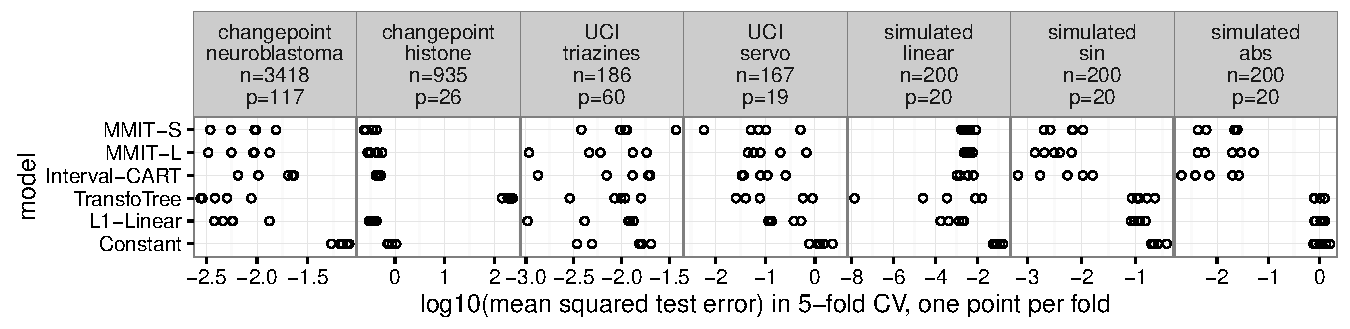
\includegraphics[width=1.1\textwidth]{figures/paper/figure-evaluate-predictions-folds.pdf}
	\end{center}
	
	\vspace{4mm}
	Metric used for comparison:
	\vspace{-2mm}
	\begin{equation*}
	\text{MSE}(h, S) = \frac{1}{n} \sum_{i=1}^n \left( [h(\xb_i) - \ylower{i}] I[h(\xb_i) < \ylower{i}] + [h(\xb_i) - \yupper{i}] I[h(\xb_i) > \yupper{i}] \right)^2
	\end{equation*}
\end{frame}

\section{Conclusion}

\begin{frame}{Conclusion}
	\begin{itemize}
		\item<+-> We proposed a new decision tree algorithm for the interval regression setting
		\vspace{3mm}
		\item<+-> We showed that such trees could be trained by solving a small number of convex optimization problems
		\vspace{3mm}
		\item<+-> We proposed an efficient dynamic programming algorithm for this task
		\vspace{3mm}
		\item<+-> Our algorithm compares favorably to the state of the art
	\end{itemize}
\end{frame}

\begin{frame}[noframenumbering]
	\begin{center}
		{\huge Thank you!}\\[20mm]
		{\huge Questions?}
	\end{center}
\end{frame}

\end{document}
